\documentclass[twoside]{book}

% Packages required by doxygen
\usepackage{fixltx2e}
\usepackage{calc}
\usepackage{doxygen}
\usepackage[export]{adjustbox} % also loads graphicx
\usepackage{graphicx}
\usepackage[utf8]{inputenc}
\usepackage{makeidx}
\usepackage{multicol}
\usepackage{multirow}
\PassOptionsToPackage{warn}{textcomp}
\usepackage{textcomp}
\usepackage[nointegrals]{wasysym}
\usepackage[table]{xcolor}

% Font selection
\usepackage[T1]{fontenc}
\usepackage[scaled=.90]{helvet}
\usepackage{courier}
\usepackage{amssymb}
\usepackage{sectsty}
\renewcommand{\familydefault}{\sfdefault}
\allsectionsfont{%
  \fontseries{bc}\selectfont%
  \color{darkgray}%
}
\renewcommand{\DoxyLabelFont}{%
  \fontseries{bc}\selectfont%
  \color{darkgray}%
}
\newcommand{\+}{\discretionary{\mbox{\scriptsize$\hookleftarrow$}}{}{}}

% Page & text layout
\usepackage{geometry}
\geometry{%
  a4paper,%
  top=2.5cm,%
  bottom=2.5cm,%
  left=2.5cm,%
  right=2.5cm%
}
\tolerance=750
\hfuzz=15pt
\hbadness=750
\setlength{\emergencystretch}{15pt}
\setlength{\parindent}{0cm}
\setlength{\parskip}{3ex plus 2ex minus 2ex}
\makeatletter
\renewcommand{\paragraph}{%
  \@startsection{paragraph}{4}{0ex}{-1.0ex}{1.0ex}{%
    \normalfont\normalsize\bfseries\SS@parafont%
  }%
}
\renewcommand{\subparagraph}{%
  \@startsection{subparagraph}{5}{0ex}{-1.0ex}{1.0ex}{%
    \normalfont\normalsize\bfseries\SS@subparafont%
  }%
}
\makeatother

% Headers & footers
\usepackage{fancyhdr}
\pagestyle{fancyplain}
\fancyhead[LE]{\fancyplain{}{\bfseries\thepage}}
\fancyhead[CE]{\fancyplain{}{}}
\fancyhead[RE]{\fancyplain{}{\bfseries\leftmark}}
\fancyhead[LO]{\fancyplain{}{\bfseries\rightmark}}
\fancyhead[CO]{\fancyplain{}{}}
\fancyhead[RO]{\fancyplain{}{\bfseries\thepage}}
\fancyfoot[LE]{\fancyplain{}{}}
\fancyfoot[CE]{\fancyplain{}{}}
\fancyfoot[RE]{\fancyplain{}{\bfseries\scriptsize Generated by Doxygen }}
\fancyfoot[LO]{\fancyplain{}{\bfseries\scriptsize Generated by Doxygen }}
\fancyfoot[CO]{\fancyplain{}{}}
\fancyfoot[RO]{\fancyplain{}{}}
\renewcommand{\footrulewidth}{0.4pt}
\renewcommand{\chaptermark}[1]{%
  \markboth{#1}{}%
}
\renewcommand{\sectionmark}[1]{%
  \markright{\thesection\ #1}%
}

% Indices & bibliography
\usepackage{natbib}
\usepackage[titles]{tocloft}
\setcounter{tocdepth}{3}
\setcounter{secnumdepth}{5}
\makeindex

% Hyperlinks (required, but should be loaded last)
\usepackage{ifpdf}
\ifpdf
  \usepackage[pdftex,pagebackref=true]{hyperref}
\else
  \usepackage[ps2pdf,pagebackref=true]{hyperref}
\fi
\hypersetup{%
  colorlinks=true,%
  linkcolor=blue,%
  citecolor=blue,%
  unicode%
}

% Custom commands
\newcommand{\clearemptydoublepage}{%
  \newpage{\pagestyle{empty}\cleardoublepage}%
}

\usepackage{caption}
\captionsetup{labelsep=space,justification=centering,font={bf},singlelinecheck=off,skip=4pt,position=top}

%===== C O N T E N T S =====

\begin{document}

% Titlepage & ToC
\hypersetup{pageanchor=false,
             bookmarksnumbered=true,
             pdfencoding=unicode
            }
\pagenumbering{alph}
\begin{titlepage}
\vspace*{7cm}
\begin{center}%
{\Large A\+ST Utilities \\[1ex]\large 0.\+10.\+1 }\\
\vspace*{1cm}
{\large Generated by Doxygen 1.8.13}\\
\end{center}
\end{titlepage}
\clearemptydoublepage
\pagenumbering{roman}
\tableofcontents
\clearemptydoublepage
\pagenumbering{arabic}
\hypersetup{pageanchor=true}

%--- Begin generated contents ---
\chapter{A\+ST Utilities (Full-\/\+A\+PI)}
\label{index}\hypertarget{index}{}The original idea to use this library in combination with the lectures {\bfseries Applied Software Engineering}, {\bfseries Interaction and Game Programming}, and {\bfseries Game Architecture} from the Media Engineering and Design (Bachelor\textquotesingle{}s program) and Interactive Media (Master\textquotesingle{}s program) at the University of Applied Sciences Upper Austria. The library has been extended with more and more functions so that it is now a valuable collection of tools for mathematics, computer graphics, digital audio processing, and last but not least for computer game development. All in a manageable and limited scope and purpose, but still quite useful.

All this has been developed to produce didactically illustrative source code. Therefore, one or the other design decision has been made in favor of readability, while performance has not been completely ignored.\hypertarget{index_ack_section}{}\section{Acknowledgement}\label{index_ack_section}
I want to extend a big thank you to Nora Loimayr for her significant help in many design decisions. She is the instructor of the exercises in the {\bfseries Applied Software Engineering} course. Therefore she not only has to use this library but also explains it to others.

I would also like to thank my students, who are ultimately the target audience, the beta testers, and the library users.\hypertarget{index_hist_sect}{}\section{Version History}\label{index_hist_sect}
This library is continuously updated and extended. The version history gives an overview of the changes this library has gone through, including the latest updates. The version history can be found on this page \hyperlink{CHANGES}{Version History}.\hypertarget{index_io_sect}{}\section{Modules}\label{index_io_sect}
A\+S\+T-\/\+Utilities currently consists of the following modules\+:


\begin{DoxyItemize}
\item \hyperlink{group__math__group}{Mathematics}
\item \hyperlink{group__gfx__group}{Graphics}
\item \hyperlink{group__input__group}{Input}
\item \hyperlink{group__srv__group}{Service}
\item \hyperlink{group__ecs__group}{Entity component system}
\item \hyperlink{group__suite2d__group}{Suite 2D}
\item \hyperlink{group__sdl__group}{Simple Direct Layer} 
\end{DoxyItemize}
\chapter{Version History}
\label{CHANGES}
\Hypertarget{CHANGES}
\section*{Version 0.\+6.\+0}

{\itshape Date\+: 2021-\/01-\/13}


\begin{DoxyItemize}
\item Removed some warnings emitted by MS compilers.
\item Fixed missing {\ttfamily \#pragma once} in Ast\+Utils0.\+h
\item Added {\ttfamily Rotate\+Deg} method to {\ttfamily Vector2} class.
\item Added class \textquotesingle{} {\ttfamily Color\+Hsv} to cover H\+SV color space as well.
\item Better encapsulation of internal functions for S\+DL applications (A\+P\+I-\/\+Level 0).
\item Added {\ttfamily Render\+Regular\+Polygon} function for S\+DL application (A\+P\+I-\/\+Level 0).
\end{DoxyItemize}

\section*{Version 0.\+5.\+3}

{\itshape Date\+: 2020-\/12-\/16}
\begin{DoxyItemize}
\item Extended {\ttfamily Color} class.
\end{DoxyItemize}

\section*{Version 0.\+5.\+2}

{\itshape Date\+: 2020-\/12-\/10}


\begin{DoxyItemize}
\item Extended {\ttfamily Vector2} template with multiplication operator between two vectors.
\item Fixed issue regarding outdated version information.
\end{DoxyItemize}

\section*{Version 0.\+5.\+1}

{\itshape Date\+: 2020-\/12-\/09}


\begin{DoxyItemize}
\item Added convenient function {\ttfamily Say\+Error()} for easy error output.
\item Refactored {\ttfamily Vector2} class to be a template class.
\item Added {\ttfamily Vector2d} alias for {\ttfamily astu\+::\+Vector2$<$double$>$}.
\item Improved support for S\+D\+L-\/based applications using A\+P\+I-\/level 0.
\end{DoxyItemize}

\section*{Version 0.\+4.\+0}

{\itshape Date\+: 2020-\/11-\/25}


\begin{DoxyItemize}
\item Added service facility for simulations and games.
\item Added Entity Component System (E\+CS) to be used for simulations and games.
\item Added template for mathematical vectors in three dimensional space.
\item Started to add basic support for S\+D\+L-\/based application for A\+P\+I-\/level 0.
\end{DoxyItemize}

\section*{Version 0.\+3.\+0}

{\itshape Date\+: 2020-\/10-\/21}


\begin{DoxyItemize}
\item Initial public release.
\item Fixed bug in ask functions causing {\ttfamily Ask\+String} not to work after calling {\ttfamily Ask\+Int} etc.
\item Improved error module.
\item Added additional math functions.
\item Fixed some issues, e.\+g, compiler warnings and errors on mac\+OS and Windows.
\item Started to work on full access level functions and classes.
\item Improved Image class.
\end{DoxyItemize}

\section*{Version 0.\+2.\+0}

{\itshape Date\+: 2020-\/08-\/19}


\begin{DoxyItemize}
\item Output methods can optionally omit end-\/of-\/line from output.
\item Added module for error handling.
\item Added module for audio processing (A\+P\+I-\/\+Level 0).
\end{DoxyItemize}

\section*{Version 0.\+1.\+0}

{\itshape Date\+: 2020-\/08-\/14}


\begin{DoxyItemize}
\item Initial version. 
\end{DoxyItemize}
\chapter{Module Index}
\section{Modules}
Here is a list of all modules\+:\begin{DoxyCompactList}
\item \contentsline{section}{Service}{\pageref{group__srv__group}}{}
\item \contentsline{section}{Entity component system}{\pageref{group__ecs__group}}{}
\item \contentsline{section}{Input}{\pageref{group__input__group}}{}
\item \contentsline{section}{Simple Direct Layer}{\pageref{group__sdl__group}}{}
\item \contentsline{section}{Graphics}{\pageref{group__gfx__group}}{}
\end{DoxyCompactList}

\chapter{Hierarchical Index}
\section{Class Hierarchy}
This inheritance list is sorted roughly, but not completely, alphabetically\+:\begin{DoxyCompactList}
\item \contentsline{section}{astu\+:\+:Color}{\pageref{classastu_1_1Color}}{}
\item enable\+\_\+shared\+\_\+from\+\_\+this\begin{DoxyCompactList}
\item \contentsline{section}{astu\+:\+:Entity}{\pageref{classastu_1_1Entity}}{}
\item \contentsline{section}{astu\+:\+:I\+Service}{\pageref{classastu_1_1IService}}{}
\begin{DoxyCompactList}
\item \contentsline{section}{astu\+:\+:Base\+Service}{\pageref{classastu_1_1BaseService}}{}
\begin{DoxyCompactList}
\item \contentsline{section}{astu\+:\+:Base\+Sdl\+Render\+Layer}{\pageref{classastu_1_1BaseSdlRenderLayer}}{}
\item \contentsline{section}{astu\+:\+:Sdl\+Service}{\pageref{classastu_1_1SdlService}}{}
\item \contentsline{section}{astu\+:\+:Sdl\+Video\+Service}{\pageref{classastu_1_1SdlVideoService}}{}
\item \contentsline{section}{astu\+:\+:State\+Service}{\pageref{classastu_1_1StateService}}{}
\item \contentsline{section}{astu\+:\+:Updatable\+Base\+Service}{\pageref{classastu_1_1UpdatableBaseService}}{}
\begin{DoxyCompactList}
\item \contentsline{section}{astu\+:\+:Entity\+Service}{\pageref{classastu_1_1EntityService}}{}
\item \contentsline{section}{astu\+:\+:Sdl\+Event\+Service}{\pageref{classastu_1_1SdlEventService}}{}
\item \contentsline{section}{astu\+:\+:Sdl\+Render\+Service}{\pageref{classastu_1_1SdlRenderService}}{}
\item \contentsline{section}{astu\+:\+:Sdl\+Time\+Service}{\pageref{classastu_1_1SdlTimeService}}{}
\item \contentsline{section}{astu\+:\+:Signal\+Service$<$ T $>$}{\pageref{classastu_1_1SignalService}}{}
\end{DoxyCompactList}
\item \contentsline{section}{astu\+:\+:Update\+Service}{\pageref{classastu_1_1UpdateService}}{}
\end{DoxyCompactList}
\end{DoxyCompactList}
\end{DoxyCompactList}
\item \contentsline{section}{astu\+:\+:Entity\+Component}{\pageref{classastu_1_1EntityComponent}}{}
\item \contentsline{section}{astu\+:\+:Entity\+Family}{\pageref{classastu_1_1EntityFamily}}{}
\item \contentsline{section}{astu\+:\+:I\+Entity\+Listener}{\pageref{classastu_1_1IEntityListener}}{}
\item \contentsline{section}{astu\+:\+:Image}{\pageref{classastu_1_1Image}}{}
\item \contentsline{section}{astu\+:\+:Image\+Renderer}{\pageref{classastu_1_1ImageRenderer}}{}
\item \contentsline{section}{astu\+:\+:I\+Sdl\+Render\+Layer}{\pageref{classastu_1_1ISdlRenderLayer}}{}
\begin{DoxyCompactList}
\item \contentsline{section}{astu\+:\+:Base\+Sdl\+Render\+Layer}{\pageref{classastu_1_1BaseSdlRenderLayer}}{}
\end{DoxyCompactList}
\item \contentsline{section}{astu\+:\+:I\+Signal\+Listener$<$ T $>$}{\pageref{classastu_1_1ISignalListener}}{}
\item \contentsline{section}{astu\+:\+:I\+Time\+Service}{\pageref{classastu_1_1ITimeService}}{}
\begin{DoxyCompactList}
\item \contentsline{section}{astu\+:\+:Sdl\+Time\+Service}{\pageref{classastu_1_1SdlTimeService}}{}
\end{DoxyCompactList}
\item \contentsline{section}{astu\+:\+:I\+Updatable}{\pageref{classastu_1_1IUpdatable}}{}
\begin{DoxyCompactList}
\item \contentsline{section}{astu\+:\+:Updatable\+Base\+Service}{\pageref{classastu_1_1UpdatableBaseService}}{}
\end{DoxyCompactList}
\item \contentsline{section}{astu\+:\+:I\+Window\+Manager}{\pageref{classastu_1_1IWindowManager}}{}
\begin{DoxyCompactList}
\item \contentsline{section}{astu\+:\+:Sdl\+Video\+Service}{\pageref{classastu_1_1SdlVideoService}}{}
\end{DoxyCompactList}
\item \contentsline{section}{astu\+:\+:Mouse}{\pageref{classastu_1_1Mouse}}{}
\item \contentsline{section}{astu\+:\+:Mouse\+Button\+Event}{\pageref{classastu_1_1MouseButtonEvent}}{}
\item \contentsline{section}{astu\+:\+:Service\+Manager}{\pageref{classastu_1_1ServiceManager}}{}
\end{DoxyCompactList}

\chapter{Class Index}
\section{Class List}
Here are the classes, structs, unions and interfaces with brief descriptions\+:\begin{DoxyCompactList}
\item\contentsline{section}{\hyperlink{classastu_1_1BaseSdlRenderLayer}{astu\+::\+Base\+Sdl\+Render\+Layer} }{\pageref{classastu_1_1BaseSdlRenderLayer}}{}
\item\contentsline{section}{\hyperlink{classastu_1_1BaseService}{astu\+::\+Base\+Service} }{\pageref{classastu_1_1BaseService}}{}
\item\contentsline{section}{\hyperlink{classastu_1_1Color}{astu\+::\+Color} }{\pageref{classastu_1_1Color}}{}
\item\contentsline{section}{\hyperlink{classastu_1_1Entity}{astu\+::\+Entity} }{\pageref{classastu_1_1Entity}}{}
\item\contentsline{section}{\hyperlink{classastu_1_1EntityComponent}{astu\+::\+Entity\+Component} }{\pageref{classastu_1_1EntityComponent}}{}
\item\contentsline{section}{\hyperlink{classastu_1_1EntityFamily}{astu\+::\+Entity\+Family} }{\pageref{classastu_1_1EntityFamily}}{}
\item\contentsline{section}{\hyperlink{classastu_1_1EntityService}{astu\+::\+Entity\+Service} }{\pageref{classastu_1_1EntityService}}{}
\item\contentsline{section}{\hyperlink{classastu_1_1IEntityListener}{astu\+::\+I\+Entity\+Listener} }{\pageref{classastu_1_1IEntityListener}}{}
\item\contentsline{section}{\hyperlink{classastu_1_1Image}{astu\+::\+Image} }{\pageref{classastu_1_1Image}}{}
\item\contentsline{section}{\hyperlink{classastu_1_1ISdlRenderLayer}{astu\+::\+I\+Sdl\+Render\+Layer} }{\pageref{classastu_1_1ISdlRenderLayer}}{}
\item\contentsline{section}{\hyperlink{classastu_1_1IService}{astu\+::\+I\+Service} }{\pageref{classastu_1_1IService}}{}
\item\contentsline{section}{\hyperlink{classastu_1_1ISignalListener}{astu\+::\+I\+Signal\+Listener$<$ T $>$} }{\pageref{classastu_1_1ISignalListener}}{}
\item\contentsline{section}{\hyperlink{classastu_1_1ITimeService}{astu\+::\+I\+Time\+Service} }{\pageref{classastu_1_1ITimeService}}{}
\item\contentsline{section}{\hyperlink{classastu_1_1IUpdatable}{astu\+::\+I\+Updatable} }{\pageref{classastu_1_1IUpdatable}}{}
\item\contentsline{section}{\hyperlink{classastu_1_1IWindowManager}{astu\+::\+I\+Window\+Manager} }{\pageref{classastu_1_1IWindowManager}}{}
\item\contentsline{section}{\hyperlink{classastu_1_1Mouse}{astu\+::\+Mouse} }{\pageref{classastu_1_1Mouse}}{}
\item\contentsline{section}{\hyperlink{classastu_1_1MouseButtonEvent}{astu\+::\+Mouse\+Button\+Event} }{\pageref{classastu_1_1MouseButtonEvent}}{}
\item\contentsline{section}{\hyperlink{classastu_1_1SdlEventService}{astu\+::\+Sdl\+Event\+Service} }{\pageref{classastu_1_1SdlEventService}}{}
\item\contentsline{section}{\hyperlink{classastu_1_1SdlRenderService}{astu\+::\+Sdl\+Render\+Service} }{\pageref{classastu_1_1SdlRenderService}}{}
\item\contentsline{section}{\hyperlink{classastu_1_1SdlService}{astu\+::\+Sdl\+Service} }{\pageref{classastu_1_1SdlService}}{}
\item\contentsline{section}{\hyperlink{classastu_1_1SdlTimeService}{astu\+::\+Sdl\+Time\+Service} }{\pageref{classastu_1_1SdlTimeService}}{}
\item\contentsline{section}{\hyperlink{classastu_1_1SdlVideoService}{astu\+::\+Sdl\+Video\+Service} }{\pageref{classastu_1_1SdlVideoService}}{}
\item\contentsline{section}{\hyperlink{classastu_1_1ServiceManager}{astu\+::\+Service\+Manager} }{\pageref{classastu_1_1ServiceManager}}{}
\item\contentsline{section}{\hyperlink{classastu_1_1SignalService}{astu\+::\+Signal\+Service$<$ T $>$} }{\pageref{classastu_1_1SignalService}}{}
\item\contentsline{section}{\hyperlink{classastu_1_1StateService}{astu\+::\+State\+Service} }{\pageref{classastu_1_1StateService}}{}
\item\contentsline{section}{\hyperlink{classastu_1_1UpdatableBaseService}{astu\+::\+Updatable\+Base\+Service} }{\pageref{classastu_1_1UpdatableBaseService}}{}
\item\contentsline{section}{\hyperlink{classastu_1_1UpdateService}{astu\+::\+Update\+Service} }{\pageref{classastu_1_1UpdateService}}{}
\end{DoxyCompactList}

\chapter{File Index}
\section{File List}
Here is a list of all documented files with brief descriptions\+:\begin{DoxyCompactList}
\item\contentsline{section}{include/\hyperlink{AstUtils0_8h}{Ast\+Utils0.\+h} \\*This file defines public functions offered by A\+ST utilities A\+P\+I-\/\+Level 0 }{\pageref{AstUtils0_8h}}{}
\item\contentsline{section}{include/\hyperlink{SdlApplication_8h}{Sdl\+Application.\+h} \\*This file defines public functions related to S\+D\+L-\/based applications using A\+ST utilities A\+P\+I-\/\+Level 0 }{\pageref{SdlApplication_8h}}{}
\end{DoxyCompactList}

\chapter{Module Documentation}
\hypertarget{group__math__group}{}\section{Mathematics}
\label{group__math__group}\index{Mathematics@{Mathematics}}


This module contains classes and functions dedicated to graphics.  


\subsection*{Classes}
\begin{DoxyCompactItemize}
\item 
class \hyperlink{classastu_1_1Interpolator1}{astu\+::\+Interpolator1$<$ T $>$}
\item 
class \hyperlink{classastu_1_1LinearInterpolator1}{astu\+::\+Linear\+Interpolator1$<$ T $>$}
\item 
class \hyperlink{classastu_1_1Line2}{astu\+::\+Line2$<$ T $>$}
\item 
class \hyperlink{classastu_1_1MathUtils}{astu\+::\+Math\+Utils}
\item 
class \hyperlink{classastu_1_1Matrix3}{astu\+::\+Matrix3$<$ T $>$}
\item 
class \hyperlink{classastu_1_1Polygon}{astu\+::\+Polygon$<$ T $>$}
\item 
class \hyperlink{classastu_1_1Random}{astu\+::\+Random}
\item 
class \hyperlink{classastu_1_1Ray2}{astu\+::\+Ray2$<$ T $>$}
\item 
class \hyperlink{classastu_1_1Segment1}{astu\+::\+Segment1$<$ T $>$}
\item 
class \hyperlink{classastu_1_1Segment2}{astu\+::\+Segment2$<$ T $>$}
\item 
class \hyperlink{classastu_1_1Transform2}{astu\+::\+Transform2$<$ T $>$}
\item 
class \hyperlink{classastu_1_1Vector2}{astu\+::\+Vector2$<$ T $>$}
\item 
class \hyperlink{classastu_1_1Vector3}{astu\+::\+Vector3$<$ T $>$}
\end{DoxyCompactItemize}
\subsection*{Typedefs}
\begin{DoxyCompactItemize}
\item 
using \hyperlink{group__math__group_ga9e9519d311982af417c5b7fd50fb4515}{astu\+::\+Line2d} = \hyperlink{classastu_1_1Line2}{astu\+::\+Line2}$<$ double $>$
\item 
using \hyperlink{group__math__group_ga6fbecdd0d3f742bdde8f5c000c3a8b5d}{astu\+::\+Line2f} = \hyperlink{classastu_1_1Line2}{astu\+::\+Line2}$<$ float $>$
\item 
using \hyperlink{group__math__group_gabc60e44721faec63659fd29e46d21522}{astu\+::\+Polygon2d} = \hyperlink{classastu_1_1Polygon}{astu\+::\+Polygon}$<$ double $>$
\item 
using \hyperlink{group__math__group_ga39ca0cd425ff5edd2a090d6997ce8c2a}{astu\+::\+Polygon2f} = \hyperlink{classastu_1_1Polygon}{astu\+::\+Polygon}$<$ float $>$
\item 
using \hyperlink{group__math__group_ga37ce0df4f800cdda11a64fa7d936a25d}{astu\+::\+Ray2d} = \hyperlink{classastu_1_1Ray2}{astu\+::\+Ray2}$<$ double $>$
\item 
using \hyperlink{group__math__group_gaa8986be7101408a7fbfdd07c73ecf8cb}{astu\+::\+Ray2f} = \hyperlink{classastu_1_1Ray2}{astu\+::\+Ray2}$<$ float $>$
\item 
using \hyperlink{group__math__group_ga3ed894c1b9f965fa9905c6f5a71ab5d4}{astu\+::\+Segment1d} = \hyperlink{classastu_1_1Segment1}{astu\+::\+Segment1}$<$ double $>$
\item 
using \hyperlink{group__math__group_gadaf20507cd638f02e10a5437a9810623}{astu\+::\+Segment1f} = \hyperlink{classastu_1_1Segment1}{astu\+::\+Segment1}$<$ float $>$
\item 
using \hyperlink{group__math__group_ga4a6a4a3ba71e40694ac08f39fa00a3bc}{astu\+::\+Segment2d} = \hyperlink{classastu_1_1Segment2}{astu\+::\+Segment2}$<$ double $>$
\item 
using \hyperlink{group__math__group_gab93de73c36660369f18786b88125e902}{astu\+::\+Segment2f} = \hyperlink{classastu_1_1Segment2}{astu\+::\+Segment2}$<$ float $>$
\item 
using \hyperlink{group__math__group_ga65979825a2f2857cba98d2d54a1df913}{astu\+::\+Transform2d} = \hyperlink{classastu_1_1Transform2}{Transform2}$<$ double $>$
\item 
using \hyperlink{group__math__group_gac67b5e9d27308a01ea8190ecb15e08fa}{astu\+::\+Transform2f} = \hyperlink{classastu_1_1Transform2}{Transform2}$<$ float $>$
\end{DoxyCompactItemize}


\subsection{Detailed Description}
This module contains classes and functions dedicated to graphics. 



\subsection{Typedef Documentation}
\mbox{\Hypertarget{group__math__group_ga9e9519d311982af417c5b7fd50fb4515}\label{group__math__group_ga9e9519d311982af417c5b7fd50fb4515}} 
\index{Mathematics@{Mathematics}!Line2d@{Line2d}}
\index{Line2d@{Line2d}!Mathematics@{Mathematics}}
\subsubsection{\texorpdfstring{Line2d}{Line2d}}
{\footnotesize\ttfamily using \hyperlink{group__math__group_ga9e9519d311982af417c5b7fd50fb4515}{astu\+::\+Line2d} = typedef \hyperlink{classastu_1_1Line2}{astu\+::\+Line2}$<$double$>$}

Type alias for \hyperlink{classastu_1_1Line2}{Line2} template using double as data type. \mbox{\Hypertarget{group__math__group_ga6fbecdd0d3f742bdde8f5c000c3a8b5d}\label{group__math__group_ga6fbecdd0d3f742bdde8f5c000c3a8b5d}} 
\index{Mathematics@{Mathematics}!Line2f@{Line2f}}
\index{Line2f@{Line2f}!Mathematics@{Mathematics}}
\subsubsection{\texorpdfstring{Line2f}{Line2f}}
{\footnotesize\ttfamily using \hyperlink{group__math__group_ga6fbecdd0d3f742bdde8f5c000c3a8b5d}{astu\+::\+Line2f} = typedef \hyperlink{classastu_1_1Line2}{astu\+::\+Line2}$<$float$>$}

Type alias for \hyperlink{classastu_1_1Segment1}{Segment1} template using float as data type. \mbox{\Hypertarget{group__math__group_gabc60e44721faec63659fd29e46d21522}\label{group__math__group_gabc60e44721faec63659fd29e46d21522}} 
\index{Mathematics@{Mathematics}!Polygon2d@{Polygon2d}}
\index{Polygon2d@{Polygon2d}!Mathematics@{Mathematics}}
\subsubsection{\texorpdfstring{Polygon2d}{Polygon2d}}
{\footnotesize\ttfamily using \hyperlink{group__math__group_gabc60e44721faec63659fd29e46d21522}{astu\+::\+Polygon2d} = typedef \hyperlink{classastu_1_1Polygon}{astu\+::\+Polygon}$<$double$>$}

Type alias for \hyperlink{classastu_1_1Polygon}{Polygon} template using double as data type.

\hyperlink{classastu_1_1Polygon}{Polygon} are ony defined in two-\/dimensional space, hence the {\ttfamily 2} in this alias is redundant. However, it fits to other naming conventions for classes that do exist in other dimensions on the one hand and on the other hand it helps to separate the {\ttfamily d} postfix from the class name. \mbox{\Hypertarget{group__math__group_ga39ca0cd425ff5edd2a090d6997ce8c2a}\label{group__math__group_ga39ca0cd425ff5edd2a090d6997ce8c2a}} 
\index{Mathematics@{Mathematics}!Polygon2f@{Polygon2f}}
\index{Polygon2f@{Polygon2f}!Mathematics@{Mathematics}}
\subsubsection{\texorpdfstring{Polygon2f}{Polygon2f}}
{\footnotesize\ttfamily using \hyperlink{group__math__group_ga39ca0cd425ff5edd2a090d6997ce8c2a}{astu\+::\+Polygon2f} = typedef \hyperlink{classastu_1_1Polygon}{astu\+::\+Polygon}$<$float$>$}

Type alias for \hyperlink{classastu_1_1Polygon}{Polygon} template using float as data type.

\hyperlink{classastu_1_1Polygon}{Polygon} are ony defined in two-\/dimensional space, hence the {\ttfamily 2} in this alias is redundant. However, it fits to other naming conventions for classes that do exist in other dimensions on the one hand and on the other hand it helps to separate the {\ttfamily f} postfix from the class name. \mbox{\Hypertarget{group__math__group_ga37ce0df4f800cdda11a64fa7d936a25d}\label{group__math__group_ga37ce0df4f800cdda11a64fa7d936a25d}} 
\index{Mathematics@{Mathematics}!Ray2d@{Ray2d}}
\index{Ray2d@{Ray2d}!Mathematics@{Mathematics}}
\subsubsection{\texorpdfstring{Ray2d}{Ray2d}}
{\footnotesize\ttfamily using \hyperlink{group__math__group_ga37ce0df4f800cdda11a64fa7d936a25d}{astu\+::\+Ray2d} = typedef \hyperlink{classastu_1_1Ray2}{astu\+::\+Ray2}$<$double$>$}

Type alias for \hyperlink{classastu_1_1Ray2}{Ray2} template using double as data type. \mbox{\Hypertarget{group__math__group_gaa8986be7101408a7fbfdd07c73ecf8cb}\label{group__math__group_gaa8986be7101408a7fbfdd07c73ecf8cb}} 
\index{Mathematics@{Mathematics}!Ray2f@{Ray2f}}
\index{Ray2f@{Ray2f}!Mathematics@{Mathematics}}
\subsubsection{\texorpdfstring{Ray2f}{Ray2f}}
{\footnotesize\ttfamily using \hyperlink{group__math__group_gaa8986be7101408a7fbfdd07c73ecf8cb}{astu\+::\+Ray2f} = typedef \hyperlink{classastu_1_1Ray2}{astu\+::\+Ray2}$<$float$>$}

Type alias for \hyperlink{classastu_1_1Ray2}{Ray2} template using float as data type. \mbox{\Hypertarget{group__math__group_ga3ed894c1b9f965fa9905c6f5a71ab5d4}\label{group__math__group_ga3ed894c1b9f965fa9905c6f5a71ab5d4}} 
\index{Mathematics@{Mathematics}!Segment1d@{Segment1d}}
\index{Segment1d@{Segment1d}!Mathematics@{Mathematics}}
\subsubsection{\texorpdfstring{Segment1d}{Segment1d}}
{\footnotesize\ttfamily using \hyperlink{group__math__group_ga3ed894c1b9f965fa9905c6f5a71ab5d4}{astu\+::\+Segment1d} = typedef \hyperlink{classastu_1_1Segment1}{astu\+::\+Segment1}$<$double$>$}

Type alias for \hyperlink{classastu_1_1Segment1}{Segment1} template using double as data type. \mbox{\Hypertarget{group__math__group_gadaf20507cd638f02e10a5437a9810623}\label{group__math__group_gadaf20507cd638f02e10a5437a9810623}} 
\index{Mathematics@{Mathematics}!Segment1f@{Segment1f}}
\index{Segment1f@{Segment1f}!Mathematics@{Mathematics}}
\subsubsection{\texorpdfstring{Segment1f}{Segment1f}}
{\footnotesize\ttfamily using \hyperlink{group__math__group_gadaf20507cd638f02e10a5437a9810623}{astu\+::\+Segment1f} = typedef \hyperlink{classastu_1_1Segment1}{astu\+::\+Segment1}$<$float$>$}

Type alias for \hyperlink{classastu_1_1Segment1}{Segment1} template using float as data type. \mbox{\Hypertarget{group__math__group_ga4a6a4a3ba71e40694ac08f39fa00a3bc}\label{group__math__group_ga4a6a4a3ba71e40694ac08f39fa00a3bc}} 
\index{Mathematics@{Mathematics}!Segment2d@{Segment2d}}
\index{Segment2d@{Segment2d}!Mathematics@{Mathematics}}
\subsubsection{\texorpdfstring{Segment2d}{Segment2d}}
{\footnotesize\ttfamily using \hyperlink{group__math__group_ga4a6a4a3ba71e40694ac08f39fa00a3bc}{astu\+::\+Segment2d} = typedef \hyperlink{classastu_1_1Segment2}{astu\+::\+Segment2}$<$double$>$}

Type alias for \hyperlink{classastu_1_1Segment2}{Segment2} template using double as data type. \mbox{\Hypertarget{group__math__group_gab93de73c36660369f18786b88125e902}\label{group__math__group_gab93de73c36660369f18786b88125e902}} 
\index{Mathematics@{Mathematics}!Segment2f@{Segment2f}}
\index{Segment2f@{Segment2f}!Mathematics@{Mathematics}}
\subsubsection{\texorpdfstring{Segment2f}{Segment2f}}
{\footnotesize\ttfamily using \hyperlink{group__math__group_gab93de73c36660369f18786b88125e902}{astu\+::\+Segment2f} = typedef \hyperlink{classastu_1_1Segment2}{astu\+::\+Segment2}$<$float$>$}

Type alias for \hyperlink{classastu_1_1Segment1}{Segment1} template using float as data type. \mbox{\Hypertarget{group__math__group_ga65979825a2f2857cba98d2d54a1df913}\label{group__math__group_ga65979825a2f2857cba98d2d54a1df913}} 
\index{Mathematics@{Mathematics}!Transform2d@{Transform2d}}
\index{Transform2d@{Transform2d}!Mathematics@{Mathematics}}
\subsubsection{\texorpdfstring{Transform2d}{Transform2d}}
{\footnotesize\ttfamily using \hyperlink{group__math__group_ga65979825a2f2857cba98d2d54a1df913}{astu\+::\+Transform2d} = typedef \hyperlink{classastu_1_1Transform2}{Transform2}$<$double$>$}

Type alias for Transform template using double as data type. \mbox{\Hypertarget{group__math__group_gac67b5e9d27308a01ea8190ecb15e08fa}\label{group__math__group_gac67b5e9d27308a01ea8190ecb15e08fa}} 
\index{Mathematics@{Mathematics}!Transform2f@{Transform2f}}
\index{Transform2f@{Transform2f}!Mathematics@{Mathematics}}
\subsubsection{\texorpdfstring{Transform2f}{Transform2f}}
{\footnotesize\ttfamily using \hyperlink{group__math__group_gac67b5e9d27308a01ea8190ecb15e08fa}{astu\+::\+Transform2f} = typedef \hyperlink{classastu_1_1Transform2}{Transform2}$<$float$>$}

Type alias for Transform template using float as data type. 
\hypertarget{group__gfx__group}{}\section{Graphics}
\label{group__gfx__group}\index{Graphics@{Graphics}}


This module contains classes and functions dedicated to graphics.  


\subsection*{Classes}
\begin{DoxyCompactItemize}
\item 
class \hyperlink{classastu_1_1Image}{astu\+::\+Image}
\item 
class \hyperlink{classastu_1_1Color}{astu\+::\+Color}
\end{DoxyCompactItemize}
\subsection*{Enumerations}
\begin{DoxyCompactItemize}
\item 
enum \hyperlink{group__gfx__group_ga6f6f9db1751e96b647084ecaedff2409}{astu\+::\+Web\+Colors} \{ \newline
\hyperlink{group__gfx__group_gga6f6f9db1751e96b647084ecaedff2409ae2e0a544fd90f604852d4c9564d64b36}{astu\+::\+White} = 0x\+F\+F\+F\+F\+FF, 
\hyperlink{group__gfx__group_gga6f6f9db1751e96b647084ecaedff2409af510d993381a675f551ace1700916ff1}{astu\+::\+Silver} = 0x\+C0\+C0\+C0, 
\hyperlink{group__gfx__group_gga6f6f9db1751e96b647084ecaedff2409a0e53834dc3a9a5407fa424d1c8f9b325}{astu\+::\+Gray} = 0x808080, 
\hyperlink{group__gfx__group_gga6f6f9db1751e96b647084ecaedff2409a5272315baf30235883a6d57cb9786bca}{astu\+::\+Black} = 0x000000, 
\newline
\hyperlink{group__gfx__group_gga6f6f9db1751e96b647084ecaedff2409a4f06dbd0c0981a97dd9279788b11a457}{astu\+::\+Red} = 0x\+F\+F0000, 
\hyperlink{group__gfx__group_gga6f6f9db1751e96b647084ecaedff2409a3b3b99e98efd19f316be1cd810845ab2}{astu\+::\+Maroon} = 0x800000, 
\hyperlink{group__gfx__group_gga6f6f9db1751e96b647084ecaedff2409ad312129d450abe89b55e91a47f21d203}{astu\+::\+Yellow} = 0x\+F\+F\+F\+F00, 
\hyperlink{group__gfx__group_gga6f6f9db1751e96b647084ecaedff2409a6f2b9ebe3c0ed5395cb551a5650e7b05}{astu\+::\+Olive} = 0x808000, 
\newline
\hyperlink{group__gfx__group_gga6f6f9db1751e96b647084ecaedff2409a865298380f9bd689bbec416267a56580}{astu\+::\+Lime} = 0x00\+F\+F00, 
\hyperlink{group__gfx__group_gga6f6f9db1751e96b647084ecaedff2409a384d49f1ac85f826658bccf8f6c778f9}{astu\+::\+Green} = 0x008000, 
\hyperlink{group__gfx__group_gga6f6f9db1751e96b647084ecaedff2409a3a60a96de57d7343338c0e5b282add56}{astu\+::\+Aqua} = 0x00\+F\+F\+FF, 
\hyperlink{group__gfx__group_gga6f6f9db1751e96b647084ecaedff2409a1d6dc387dfdc24340027139fa56c8bbd}{astu\+::\+Teal} = 0x008080, 
\newline
\hyperlink{group__gfx__group_gga6f6f9db1751e96b647084ecaedff2409a62679f040a4e55584b1bf519be06fbde}{astu\+::\+Blue} = 0x0000\+FF, 
\hyperlink{group__gfx__group_gga6f6f9db1751e96b647084ecaedff2409a97810f1c2418830c1e7f556c2a63e9e5}{astu\+::\+Navy} = 0x000080, 
\hyperlink{group__gfx__group_gga6f6f9db1751e96b647084ecaedff2409ae7ff5f29f6e8830d96b791c698b57f18}{astu\+::\+Fuchsia} = 0x\+F\+F00\+FF, 
\hyperlink{group__gfx__group_gga6f6f9db1751e96b647084ecaedff2409a01a986e72b737c665011360937fc2e52}{astu\+::\+Purple} = 0x800080
 \}
\end{DoxyCompactItemize}
\subsection*{Functions}
\begin{DoxyCompactItemize}
\item 
void \hyperlink{group__gfx__group_gaca5f9cb8047c60049300242c20d30cd6}{astu\+::\+Store\+Image} (const \hyperlink{classastu_1_1Image}{Image} \&image, const std\+::string \&filename)
\item 
std\+::unique\+\_\+ptr$<$ \hyperlink{classastu_1_1Image}{Image} $>$ \hyperlink{group__gfx__group_ga46ac561eac42d4ace785797db8bc89a0}{astu\+::\+Load\+Image} (const std\+::string \&filename)
\end{DoxyCompactItemize}


\subsection{Detailed Description}
This module contains classes and functions dedicated to graphics. 



\subsection{Enumeration Type Documentation}
\mbox{\Hypertarget{group__gfx__group_ga6f6f9db1751e96b647084ecaedff2409}\label{group__gfx__group_ga6f6f9db1751e96b647084ecaedff2409}} 
\index{Graphics@{Graphics}!Web\+Colors@{Web\+Colors}}
\index{Web\+Colors@{Web\+Colors}!Graphics@{Graphics}}
\subsubsection{\texorpdfstring{Web\+Colors}{WebColors}}
{\footnotesize\ttfamily enum \hyperlink{group__gfx__group_ga6f6f9db1751e96b647084ecaedff2409}{astu\+::\+Web\+Colors}}

This enumeration defines values for color names according to the W3C specification. \begin{DoxyEnumFields}{Enumerator}
\raisebox{\heightof{T}}[0pt][0pt]{\index{White@{White}!Graphics@{Graphics}}\index{Graphics@{Graphics}!White@{White}}}\mbox{\Hypertarget{group__gfx__group_gga6f6f9db1751e96b647084ecaedff2409ae2e0a544fd90f604852d4c9564d64b36}\label{group__gfx__group_gga6f6f9db1751e96b647084ecaedff2409ae2e0a544fd90f604852d4c9564d64b36}} 
White&\hyperlink{classastu_1_1Color}{Color} constant for the color {\itshape White} (0x\+F\+F\+F\+F\+FF). \\
\hline

\raisebox{\heightof{T}}[0pt][0pt]{\index{Silver@{Silver}!Graphics@{Graphics}}\index{Graphics@{Graphics}!Silver@{Silver}}}\mbox{\Hypertarget{group__gfx__group_gga6f6f9db1751e96b647084ecaedff2409af510d993381a675f551ace1700916ff1}\label{group__gfx__group_gga6f6f9db1751e96b647084ecaedff2409af510d993381a675f551ace1700916ff1}} 
Silver&\hyperlink{classastu_1_1Color}{Color} constant for the color {\itshape Silver} (0x\+C0\+C0\+C0). \\
\hline

\raisebox{\heightof{T}}[0pt][0pt]{\index{Gray@{Gray}!Graphics@{Graphics}}\index{Graphics@{Graphics}!Gray@{Gray}}}\mbox{\Hypertarget{group__gfx__group_gga6f6f9db1751e96b647084ecaedff2409a0e53834dc3a9a5407fa424d1c8f9b325}\label{group__gfx__group_gga6f6f9db1751e96b647084ecaedff2409a0e53834dc3a9a5407fa424d1c8f9b325}} 
Gray&\hyperlink{classastu_1_1Color}{Color} constant for the color {\itshape Gray} (0x808080). \\
\hline

\raisebox{\heightof{T}}[0pt][0pt]{\index{Black@{Black}!Graphics@{Graphics}}\index{Graphics@{Graphics}!Black@{Black}}}\mbox{\Hypertarget{group__gfx__group_gga6f6f9db1751e96b647084ecaedff2409a5272315baf30235883a6d57cb9786bca}\label{group__gfx__group_gga6f6f9db1751e96b647084ecaedff2409a5272315baf30235883a6d57cb9786bca}} 
Black&\hyperlink{classastu_1_1Color}{Color} constant for the color {\itshape Black} (0x000000). \\
\hline

\raisebox{\heightof{T}}[0pt][0pt]{\index{Red@{Red}!Graphics@{Graphics}}\index{Graphics@{Graphics}!Red@{Red}}}\mbox{\Hypertarget{group__gfx__group_gga6f6f9db1751e96b647084ecaedff2409a4f06dbd0c0981a97dd9279788b11a457}\label{group__gfx__group_gga6f6f9db1751e96b647084ecaedff2409a4f06dbd0c0981a97dd9279788b11a457}} 
Red&\hyperlink{classastu_1_1Color}{Color} constant for the color {\itshape Red} (0x\+F\+F0000). \\
\hline

\raisebox{\heightof{T}}[0pt][0pt]{\index{Maroon@{Maroon}!Graphics@{Graphics}}\index{Graphics@{Graphics}!Maroon@{Maroon}}}\mbox{\Hypertarget{group__gfx__group_gga6f6f9db1751e96b647084ecaedff2409a3b3b99e98efd19f316be1cd810845ab2}\label{group__gfx__group_gga6f6f9db1751e96b647084ecaedff2409a3b3b99e98efd19f316be1cd810845ab2}} 
Maroon&\hyperlink{classastu_1_1Color}{Color} constant for the color {\itshape Maroon} (0x800000). \\
\hline

\raisebox{\heightof{T}}[0pt][0pt]{\index{Yellow@{Yellow}!Graphics@{Graphics}}\index{Graphics@{Graphics}!Yellow@{Yellow}}}\mbox{\Hypertarget{group__gfx__group_gga6f6f9db1751e96b647084ecaedff2409ad312129d450abe89b55e91a47f21d203}\label{group__gfx__group_gga6f6f9db1751e96b647084ecaedff2409ad312129d450abe89b55e91a47f21d203}} 
Yellow&\hyperlink{classastu_1_1Color}{Color} constant for the color {\itshape Yellow} (0x\+F\+F\+F\+F00). \\
\hline

\raisebox{\heightof{T}}[0pt][0pt]{\index{Olive@{Olive}!Graphics@{Graphics}}\index{Graphics@{Graphics}!Olive@{Olive}}}\mbox{\Hypertarget{group__gfx__group_gga6f6f9db1751e96b647084ecaedff2409a6f2b9ebe3c0ed5395cb551a5650e7b05}\label{group__gfx__group_gga6f6f9db1751e96b647084ecaedff2409a6f2b9ebe3c0ed5395cb551a5650e7b05}} 
Olive&\hyperlink{classastu_1_1Color}{Color} constant for the color {\itshape Olive} (0x808000). \\
\hline

\raisebox{\heightof{T}}[0pt][0pt]{\index{Lime@{Lime}!Graphics@{Graphics}}\index{Graphics@{Graphics}!Lime@{Lime}}}\mbox{\Hypertarget{group__gfx__group_gga6f6f9db1751e96b647084ecaedff2409a865298380f9bd689bbec416267a56580}\label{group__gfx__group_gga6f6f9db1751e96b647084ecaedff2409a865298380f9bd689bbec416267a56580}} 
Lime&\hyperlink{classastu_1_1Color}{Color} constant for the color {\itshape Lime} (0x00\+F\+F00). \\
\hline

\raisebox{\heightof{T}}[0pt][0pt]{\index{Green@{Green}!Graphics@{Graphics}}\index{Graphics@{Graphics}!Green@{Green}}}\mbox{\Hypertarget{group__gfx__group_gga6f6f9db1751e96b647084ecaedff2409a384d49f1ac85f826658bccf8f6c778f9}\label{group__gfx__group_gga6f6f9db1751e96b647084ecaedff2409a384d49f1ac85f826658bccf8f6c778f9}} 
Green&\hyperlink{classastu_1_1Color}{Color} constant for the color {\itshape Green} (0x008000). \\
\hline

\raisebox{\heightof{T}}[0pt][0pt]{\index{Aqua@{Aqua}!Graphics@{Graphics}}\index{Graphics@{Graphics}!Aqua@{Aqua}}}\mbox{\Hypertarget{group__gfx__group_gga6f6f9db1751e96b647084ecaedff2409a3a60a96de57d7343338c0e5b282add56}\label{group__gfx__group_gga6f6f9db1751e96b647084ecaedff2409a3a60a96de57d7343338c0e5b282add56}} 
Aqua&\hyperlink{classastu_1_1Color}{Color} constant for the color {\itshape Aqua} (0x00\+F\+F\+FF). \\
\hline

\raisebox{\heightof{T}}[0pt][0pt]{\index{Teal@{Teal}!Graphics@{Graphics}}\index{Graphics@{Graphics}!Teal@{Teal}}}\mbox{\Hypertarget{group__gfx__group_gga6f6f9db1751e96b647084ecaedff2409a1d6dc387dfdc24340027139fa56c8bbd}\label{group__gfx__group_gga6f6f9db1751e96b647084ecaedff2409a1d6dc387dfdc24340027139fa56c8bbd}} 
Teal&\hyperlink{classastu_1_1Color}{Color} constant for the color {\itshape Teal} (0x008080). \\
\hline

\raisebox{\heightof{T}}[0pt][0pt]{\index{Blue@{Blue}!Graphics@{Graphics}}\index{Graphics@{Graphics}!Blue@{Blue}}}\mbox{\Hypertarget{group__gfx__group_gga6f6f9db1751e96b647084ecaedff2409a62679f040a4e55584b1bf519be06fbde}\label{group__gfx__group_gga6f6f9db1751e96b647084ecaedff2409a62679f040a4e55584b1bf519be06fbde}} 
Blue&\hyperlink{classastu_1_1Color}{Color} constant for the color {\itshape Blue} (0x0000\+FF). \\
\hline

\raisebox{\heightof{T}}[0pt][0pt]{\index{Navy@{Navy}!Graphics@{Graphics}}\index{Graphics@{Graphics}!Navy@{Navy}}}\mbox{\Hypertarget{group__gfx__group_gga6f6f9db1751e96b647084ecaedff2409a97810f1c2418830c1e7f556c2a63e9e5}\label{group__gfx__group_gga6f6f9db1751e96b647084ecaedff2409a97810f1c2418830c1e7f556c2a63e9e5}} 
Navy&\hyperlink{classastu_1_1Color}{Color} constant for the color {\itshape Navy} (0x000080). \\
\hline

\raisebox{\heightof{T}}[0pt][0pt]{\index{Fuchsia@{Fuchsia}!Graphics@{Graphics}}\index{Graphics@{Graphics}!Fuchsia@{Fuchsia}}}\mbox{\Hypertarget{group__gfx__group_gga6f6f9db1751e96b647084ecaedff2409ae7ff5f29f6e8830d96b791c698b57f18}\label{group__gfx__group_gga6f6f9db1751e96b647084ecaedff2409ae7ff5f29f6e8830d96b791c698b57f18}} 
Fuchsia&\hyperlink{classastu_1_1Color}{Color} constant for the color {\itshape Fuchsia} (0x\+F\+F00\+FF). \\
\hline

\raisebox{\heightof{T}}[0pt][0pt]{\index{Purple@{Purple}!Graphics@{Graphics}}\index{Graphics@{Graphics}!Purple@{Purple}}}\mbox{\Hypertarget{group__gfx__group_gga6f6f9db1751e96b647084ecaedff2409a01a986e72b737c665011360937fc2e52}\label{group__gfx__group_gga6f6f9db1751e96b647084ecaedff2409a01a986e72b737c665011360937fc2e52}} 
Purple&\hyperlink{classastu_1_1Color}{Color} constant for the color {\itshape Purple} (0x800080). \\
\hline

\end{DoxyEnumFields}


\subsection{Function Documentation}
\mbox{\Hypertarget{group__gfx__group_ga46ac561eac42d4ace785797db8bc89a0}\label{group__gfx__group_ga46ac561eac42d4ace785797db8bc89a0}} 
\index{Graphics@{Graphics}!Load\+Image@{Load\+Image}}
\index{Load\+Image@{Load\+Image}!Graphics@{Graphics}}
\subsubsection{\texorpdfstring{Load\+Image()}{LoadImage()}}
{\footnotesize\ttfamily std\+::unique\+\_\+ptr$<$\hyperlink{classastu_1_1Image}{Image}$>$ astu\+::\+Load\+Image (\begin{DoxyParamCaption}\item[{const std\+::string \&}]{filename }\end{DoxyParamCaption})}

Loads an B\+MP image from file.


\begin{DoxyParams}{Parameters}
{\em filename} & the filename including the path \\
\hline
\end{DoxyParams}
\begin{DoxyReturn}{Returns}
the loaded image 
\end{DoxyReturn}

\begin{DoxyExceptions}{Exceptions}
{\em std\+::runtime\+\_\+error} & in case of an I/O error \\
\hline
\end{DoxyExceptions}
\mbox{\Hypertarget{group__gfx__group_gaca5f9cb8047c60049300242c20d30cd6}\label{group__gfx__group_gaca5f9cb8047c60049300242c20d30cd6}} 
\index{Graphics@{Graphics}!Store\+Image@{Store\+Image}}
\index{Store\+Image@{Store\+Image}!Graphics@{Graphics}}
\subsubsection{\texorpdfstring{Store\+Image()}{StoreImage()}}
{\footnotesize\ttfamily void astu\+::\+Store\+Image (\begin{DoxyParamCaption}\item[{const \hyperlink{classastu_1_1Image}{Image} \&}]{image,  }\item[{const std\+::string \&}]{filename }\end{DoxyParamCaption})}

Stores an image as B\+MP file.


\begin{DoxyParams}{Parameters}
{\em image} & the the image to be stored \\
\hline
{\em filename} & the filename including the path \\
\hline
\end{DoxyParams}

\begin{DoxyExceptions}{Exceptions}
{\em std\+::runtime\+\_\+error} & in case of an I/O error \\
\hline
\end{DoxyExceptions}

\hypertarget{group__input__group}{}\section{Input}
\label{group__input__group}\index{Input@{Input}}


This module contains templates, classes and functions dedicated user input.  


\subsection*{Classes}
\begin{DoxyCompactItemize}
\item 
class \hyperlink{classastu_1_1Mouse}{astu\+::\+Mouse}
\item 
class \hyperlink{classastu_1_1MouseButtonEvent}{astu\+::\+Mouse\+Button\+Event}
\end{DoxyCompactItemize}
\subsection*{Typedefs}
\begin{DoxyCompactItemize}
\item 
using \hyperlink{group__input__group_ga720d9f880198971a77aad9ba69cc3633}{astu\+::\+Mouse\+Button\+Event\+Service} = \hyperlink{classastu_1_1SignalService}{Signal\+Service}$<$ \hyperlink{classastu_1_1MouseButtonEvent}{Mouse\+Button\+Event} $>$
\item 
using \hyperlink{group__input__group_ga4358d168fa211f641ec8176f279f421b}{astu\+::\+Mouse\+Button\+Listener} = \hyperlink{classastu_1_1ISignalListener}{I\+Signal\+Listener}$<$ \hyperlink{classastu_1_1MouseButtonEvent}{Mouse\+Button\+Event} $>$
\end{DoxyCompactItemize}


\subsection{Detailed Description}
This module contains templates, classes and functions dedicated user input. 



\subsection{Typedef Documentation}
\mbox{\Hypertarget{group__input__group_ga720d9f880198971a77aad9ba69cc3633}\label{group__input__group_ga720d9f880198971a77aad9ba69cc3633}} 
\index{Input@{Input}!Mouse\+Button\+Event\+Service@{Mouse\+Button\+Event\+Service}}
\index{Mouse\+Button\+Event\+Service@{Mouse\+Button\+Event\+Service}!Input@{Input}}
\subsubsection{\texorpdfstring{Mouse\+Button\+Event\+Service}{MouseButtonEventService}}
{\footnotesize\ttfamily using \hyperlink{group__input__group_ga720d9f880198971a77aad9ba69cc3633}{astu\+::\+Mouse\+Button\+Event\+Service} = typedef \hyperlink{classastu_1_1SignalService}{Signal\+Service}$<$\hyperlink{classastu_1_1MouseButtonEvent}{Mouse\+Button\+Event}$>$}

Type definition for signal services used to transmit mouse button events. \mbox{\Hypertarget{group__input__group_ga4358d168fa211f641ec8176f279f421b}\label{group__input__group_ga4358d168fa211f641ec8176f279f421b}} 
\index{Input@{Input}!Mouse\+Button\+Listener@{Mouse\+Button\+Listener}}
\index{Mouse\+Button\+Listener@{Mouse\+Button\+Listener}!Input@{Input}}
\subsubsection{\texorpdfstring{Mouse\+Button\+Listener}{MouseButtonListener}}
{\footnotesize\ttfamily using \hyperlink{group__input__group_ga4358d168fa211f641ec8176f279f421b}{astu\+::\+Mouse\+Button\+Listener} = typedef \hyperlink{classastu_1_1ISignalListener}{I\+Signal\+Listener}$<$\hyperlink{classastu_1_1MouseButtonEvent}{Mouse\+Button\+Event}$>$}

Type definition for signal listeners which receive mouse button events. 
\hypertarget{group__srv__group}{}\section{Service}
\label{group__srv__group}\index{Service@{Service}}


This module contains templates, classes and functions dedicated to services.  


\subsection*{Classes}
\begin{DoxyCompactItemize}
\item 
class \hyperlink{classastu_1_1ActionSignalService}{astu\+::\+Action\+Signal\+Service}
\item 
class \hyperlink{classastu_1_1InteractiveApplication}{astu\+::\+Interactive\+Application}
\item 
class \hyperlink{classastu_1_1RenderService}{astu\+::\+Render\+Service}
\item 
class \hyperlink{classastu_1_1Service}{astu\+::\+Service}
\item 
class \hyperlink{classastu_1_1BaseService}{astu\+::\+Base\+Service}
\item 
class \hyperlink{classastu_1_1ServiceManager}{astu\+::\+Service\+Manager}
\item 
class \hyperlink{classastu_1_1ISignalListener}{astu\+::\+I\+Signal\+Listener$<$ T $>$}
\item 
class \hyperlink{classastu_1_1SignalService}{astu\+::\+Signal\+Service$<$ T $>$}
\item 
class \hyperlink{classastu_1_1SignalListener}{astu\+::\+Signal\+Listener$<$ T $>$}
\item 
class \hyperlink{classastu_1_1StateService}{astu\+::\+State\+Service}
\item 
class \hyperlink{classastu_1_1TimedTask}{astu\+::\+Timed\+Task}
\item 
class \hyperlink{classastu_1_1DelegateTaskBuilder}{astu\+::\+Delegate\+Task\+Builder}
\item 
class \hyperlink{classastu_1_1Task}{astu\+::\+Task}
\item 
class \hyperlink{classastu_1_1TaskBuilder}{astu\+::\+Task\+Builder$<$ T $>$}
\item 
class \hyperlink{classastu_1_1TaskService}{astu\+::\+Task\+Service}
\item 
class \hyperlink{classastu_1_1TimeService}{astu\+::\+Time\+Service}
\item 
class \hyperlink{classastu_1_1TimeClient}{astu\+::\+Time\+Client}
\item 
class \hyperlink{classastu_1_1IUpdatable}{astu\+::\+I\+Updatable}
\item 
class \hyperlink{classastu_1_1UpdateService}{astu\+::\+Update\+Service}
\item 
class \hyperlink{classastu_1_1Updatable}{astu\+::\+Updatable}
\item 
class \hyperlink{classastu_1_1WindowService}{astu\+::\+Window\+Service}
\end{DoxyCompactItemize}
\subsection*{Macros}
\begin{DoxyCompactItemize}
\item 
\#define \hyperlink{group__srv__group_ga5216c57cf872d6a0c05d0e6f33c66fc7}{A\+S\+T\+U\+\_\+\+S\+E\+R\+V\+I\+C\+E\+\_\+\+M\+A\+N\+A\+G\+ER}()~\hyperlink{classastu_1_1ServiceManager_a26941fe98ea3f2792deca62e4124bf15}{astu\+::\+Service\+Manager\+::\+Get\+Instance}()
\item 
\#define \hyperlink{group__srv__group_ga42575546f01bf92989d08916564ffc66}{A\+S\+T\+U\+\_\+\+S\+E\+R\+V\+I\+CE}(type)~($\ast$\hyperlink{group__srv__group_ga5216c57cf872d6a0c05d0e6f33c66fc7}{A\+S\+T\+U\+\_\+\+S\+E\+R\+V\+I\+C\+E\+\_\+\+M\+A\+N\+A\+G\+ER}().Find\+Service$<$type$>$())
\item 
\#define \hyperlink{group__srv__group_ga42e4ee34b527cd82ba6c0013b5d1441e}{A\+S\+T\+U\+\_\+\+G\+E\+T\+\_\+\+S\+E\+R\+V\+I\+CE}(type)~\hyperlink{group__srv__group_ga5216c57cf872d6a0c05d0e6f33c66fc7}{A\+S\+T\+U\+\_\+\+S\+E\+R\+V\+I\+C\+E\+\_\+\+M\+A\+N\+A\+G\+ER}().Find\+Service$<$type$>$()
\item 
\#define \hyperlink{group__srv__group_gadd58983b12766275d79b748307fcd637}{A\+S\+T\+U\+\_\+\+G\+E\+T\+\_\+\+S\+E\+R\+V\+I\+C\+E\+\_\+\+O\+R\+\_\+\+D\+E\+F\+A\+U\+LT}(type,  b)~\hyperlink{group__srv__group_ga5216c57cf872d6a0c05d0e6f33c66fc7}{A\+S\+T\+U\+\_\+\+S\+E\+R\+V\+I\+C\+E\+\_\+\+M\+A\+N\+A\+G\+ER}().Find\+Service$<$type$>$(b)
\item 
\#define \hyperlink{group__srv__group_ga223765690bb6ade99e1e5f954f096cfb}{A\+S\+T\+U\+\_\+\+G\+E\+T\+\_\+\+S\+E\+R\+V\+I\+C\+E\+\_\+\+O\+R\+\_\+\+N\+U\+LL}(type)~\hyperlink{group__srv__group_ga5216c57cf872d6a0c05d0e6f33c66fc7}{A\+S\+T\+U\+\_\+\+S\+E\+R\+V\+I\+C\+E\+\_\+\+M\+A\+N\+A\+G\+ER}().Find\+Service$<$type$>$(nullptr)
\item 
\#define \hyperlink{group__srv__group_ga8b3cd4edfd24593b12bc662acf62e9a1}{A\+S\+T\+U\+\_\+\+H\+A\+S\+\_\+\+S\+E\+R\+V\+I\+CE}(type)~(\hyperlink{group__srv__group_ga223765690bb6ade99e1e5f954f096cfb}{A\+S\+T\+U\+\_\+\+G\+E\+T\+\_\+\+S\+E\+R\+V\+I\+C\+E\+\_\+\+O\+R\+\_\+\+N\+U\+LL}(type) != nullptr)
\item 
\#define \hyperlink{group__srv__group_ga640af14a801ce66a6286ca8bc4862473}{A\+S\+T\+U\+\_\+\+R\+E\+M\+O\+V\+E\+\_\+\+A\+L\+L\+\_\+\+S\+E\+R\+V\+I\+C\+ES}()~\hyperlink{group__srv__group_ga5216c57cf872d6a0c05d0e6f33c66fc7}{A\+S\+T\+U\+\_\+\+S\+E\+R\+V\+I\+C\+E\+\_\+\+M\+A\+N\+A\+G\+ER}().Remove\+All\+Services()
\item 
\#define \hyperlink{group__srv__group_gab16fd0e9f158b318812197ee283a8484}{A\+S\+T\+U\+\_\+\+S\+T\+A\+R\+T\+U\+P\+\_\+\+S\+E\+R\+V\+I\+C\+ES}()~\hyperlink{group__srv__group_ga5216c57cf872d6a0c05d0e6f33c66fc7}{A\+S\+T\+U\+\_\+\+S\+E\+R\+V\+I\+C\+E\+\_\+\+M\+A\+N\+A\+G\+ER}().Startup\+All()
\item 
\#define \hyperlink{group__srv__group_ga97369e673940c499b1cd623c76aaafe5}{A\+S\+T\+U\+\_\+\+S\+H\+U\+T\+D\+O\+W\+N\+\_\+\+S\+E\+R\+V\+I\+C\+ES}()~\hyperlink{group__srv__group_ga5216c57cf872d6a0c05d0e6f33c66fc7}{A\+S\+T\+U\+\_\+\+S\+E\+R\+V\+I\+C\+E\+\_\+\+M\+A\+N\+A\+G\+ER}().Shutdown\+All()
\item 
\#define \hyperlink{group__srv__group_ga8c6572c2ee70b67d9dda0b8b0d77a7d2}{A\+S\+T\+U\+\_\+\+A\+D\+D\+\_\+\+S\+E\+R\+V\+I\+CE}(srv)~\hyperlink{group__srv__group_ga5216c57cf872d6a0c05d0e6f33c66fc7}{A\+S\+T\+U\+\_\+\+S\+E\+R\+V\+I\+C\+E\+\_\+\+M\+A\+N\+A\+G\+ER}().Add\+Service(srv)
\item 
\#define \hyperlink{group__srv__group_ga91256015ad12618b8eda42106056a927}{A\+S\+T\+U\+\_\+\+C\+R\+E\+A\+T\+E\+\_\+\+A\+N\+D\+\_\+\+A\+D\+D\+\_\+\+S\+E\+R\+V\+I\+CE}(srv\+Type, ...)~if(!\hyperlink{group__srv__group_ga8b3cd4edfd24593b12bc662acf62e9a1}{A\+S\+T\+U\+\_\+\+H\+A\+S\+\_\+\+S\+E\+R\+V\+I\+CE}(srv\+Type)) \hyperlink{group__srv__group_ga8c6572c2ee70b67d9dda0b8b0d77a7d2}{A\+S\+T\+U\+\_\+\+A\+D\+D\+\_\+\+S\+E\+R\+V\+I\+CE}(std\+::make\+\_\+shared$<$srv\+Type$>$(\+\_\+\+\_\+\+V\+A\+\_\+\+A\+R\+G\+S\+\_\+\+\_\+) )
\end{DoxyCompactItemize}
\subsection*{Enumerations}
\begin{DoxyCompactItemize}
\item 
enum \hyperlink{group__srv__group_gaf164c3f1c393e1f240458ae4fcd484a0}{astu\+::\+Priority} \{ \newline
{\bfseries Very\+High} = 0, 
{\bfseries High} = 500, 
{\bfseries Normal} = 1000, 
{\bfseries Low} = 1500, 
\newline
{\bfseries Very\+Low} = 2000
 \}
\item 
enum \hyperlink{group__srv__group_ga68a91c7015964dbdea802829ae5ccb3c}{astu\+::\+Resolution} \{ \newline
\hyperlink{group__srv__group_gga68a91c7015964dbdea802829ae5ccb3ca55a1cd59378161f3d8d162f7ab3c688c}{astu\+::\+Resolution\+::\+S\+V\+GA}, 
\hyperlink{group__srv__group_gga68a91c7015964dbdea802829ae5ccb3ca8d1b2ed4d604a6be96ad2f218592b98e}{astu\+::\+Resolution\+::\+X\+GA}, 
\hyperlink{group__srv__group_gga68a91c7015964dbdea802829ae5ccb3ca521265ba830a9825dd75ac96bffc3c04}{astu\+::\+Resolution\+::\+W\+X\+GA}, 
\hyperlink{group__srv__group_gga68a91c7015964dbdea802829ae5ccb3ca0b8f37f43da5e66c4bd58165b40b76f3}{astu\+::\+Resolution\+::\+S\+X\+GA}, 
\newline
\hyperlink{group__srv__group_gga68a91c7015964dbdea802829ae5ccb3ca5f825911c42fe77eab9de44602f7080e}{astu\+::\+Resolution\+::\+H\+D\+\_\+1}, 
\hyperlink{group__srv__group_gga68a91c7015964dbdea802829ae5ccb3ca0019cdc8d430b07dccbbe6453de8f244}{astu\+::\+Resolution\+::\+H\+D\+\_\+2}, 
\hyperlink{group__srv__group_gga68a91c7015964dbdea802829ae5ccb3ca188ce673037fb8cc15ef18b2db6b470b}{astu\+::\+Resolution\+::\+W\+X\+G\+A\+\_\+\+P\+L\+US}, 
\hyperlink{group__srv__group_gga68a91c7015964dbdea802829ae5ccb3ca95c1d10ada9f6c64467275175334744b}{astu\+::\+Resolution\+::\+W\+S\+X\+G\+A\+\_\+\+P\+L\+US}, 
\newline
\hyperlink{group__srv__group_gga68a91c7015964dbdea802829ae5ccb3ca7ff9eb087b5873e5245422ffc8e6f054}{astu\+::\+Resolution\+::\+F\+HD}, 
\hyperlink{group__srv__group_gga68a91c7015964dbdea802829ae5ccb3ca512db9ef494be9c910409a51fbc9eb9c}{astu\+::\+Resolution\+::\+Q\+HD}, 
\hyperlink{group__srv__group_gga68a91c7015964dbdea802829ae5ccb3cab61f857a573f21f72e277339f072402b}{astu\+::\+Resolution\+::\+W\+I\+D\+E\+\_\+\+S\+C\+R\+E\+EN}, 
\hyperlink{group__srv__group_gga68a91c7015964dbdea802829ae5ccb3ca9a4d0ff86f135b89378b858a0d947483}{astu\+::\+Resolution\+::\+U\+H\+D\+\_\+4K}
 \}
\end{DoxyCompactItemize}


\subsection{Detailed Description}
This module contains templates, classes and functions dedicated to services. 



\subsection{Macro Definition Documentation}
\mbox{\Hypertarget{group__srv__group_ga8c6572c2ee70b67d9dda0b8b0d77a7d2}\label{group__srv__group_ga8c6572c2ee70b67d9dda0b8b0d77a7d2}} 
\index{Service@{Service}!A\+S\+T\+U\+\_\+\+A\+D\+D\+\_\+\+S\+E\+R\+V\+I\+CE@{A\+S\+T\+U\+\_\+\+A\+D\+D\+\_\+\+S\+E\+R\+V\+I\+CE}}
\index{A\+S\+T\+U\+\_\+\+A\+D\+D\+\_\+\+S\+E\+R\+V\+I\+CE@{A\+S\+T\+U\+\_\+\+A\+D\+D\+\_\+\+S\+E\+R\+V\+I\+CE}!Service@{Service}}
\subsubsection{\texorpdfstring{A\+S\+T\+U\+\_\+\+A\+D\+D\+\_\+\+S\+E\+R\+V\+I\+CE}{ASTU\_ADD\_SERVICE}}
{\footnotesize\ttfamily \#define A\+S\+T\+U\+\_\+\+A\+D\+D\+\_\+\+S\+E\+R\+V\+I\+CE(\begin{DoxyParamCaption}\item[{}]{srv }\end{DoxyParamCaption})~\hyperlink{group__srv__group_ga5216c57cf872d6a0c05d0e6f33c66fc7}{A\+S\+T\+U\+\_\+\+S\+E\+R\+V\+I\+C\+E\+\_\+\+M\+A\+N\+A\+G\+ER}().Add\+Service(srv)}

Adds a new service to the service manager.

{\bfseries Example}


\begin{DoxyCode}
\hyperlink{group__srv__group_ga8c6572c2ee70b67d9dda0b8b0d77a7d2}{ASTU\_ADD\_SERVICE}( std::make\_shared<SignalService<int>>() );
\end{DoxyCode}



\begin{DoxyParams}{Parameters}
{\em srv} & the service to add \\
\hline
\end{DoxyParams}

\begin{DoxyExceptions}{Exceptions}
{\em std\+::runtime\+\_\+error} & in case the service has alerady been added \\
\hline
\end{DoxyExceptions}
\mbox{\Hypertarget{group__srv__group_ga91256015ad12618b8eda42106056a927}\label{group__srv__group_ga91256015ad12618b8eda42106056a927}} 
\index{Service@{Service}!A\+S\+T\+U\+\_\+\+C\+R\+E\+A\+T\+E\+\_\+\+A\+N\+D\+\_\+\+A\+D\+D\+\_\+\+S\+E\+R\+V\+I\+CE@{A\+S\+T\+U\+\_\+\+C\+R\+E\+A\+T\+E\+\_\+\+A\+N\+D\+\_\+\+A\+D\+D\+\_\+\+S\+E\+R\+V\+I\+CE}}
\index{A\+S\+T\+U\+\_\+\+C\+R\+E\+A\+T\+E\+\_\+\+A\+N\+D\+\_\+\+A\+D\+D\+\_\+\+S\+E\+R\+V\+I\+CE@{A\+S\+T\+U\+\_\+\+C\+R\+E\+A\+T\+E\+\_\+\+A\+N\+D\+\_\+\+A\+D\+D\+\_\+\+S\+E\+R\+V\+I\+CE}!Service@{Service}}
\subsubsection{\texorpdfstring{A\+S\+T\+U\+\_\+\+C\+R\+E\+A\+T\+E\+\_\+\+A\+N\+D\+\_\+\+A\+D\+D\+\_\+\+S\+E\+R\+V\+I\+CE}{ASTU\_CREATE\_AND\_ADD\_SERVICE}}
{\footnotesize\ttfamily \#define A\+S\+T\+U\+\_\+\+C\+R\+E\+A\+T\+E\+\_\+\+A\+N\+D\+\_\+\+A\+D\+D\+\_\+\+S\+E\+R\+V\+I\+CE(\begin{DoxyParamCaption}\item[{}]{srv\+Type,  }\item[{}]{... }\end{DoxyParamCaption})~if(!\hyperlink{group__srv__group_ga8b3cd4edfd24593b12bc662acf62e9a1}{A\+S\+T\+U\+\_\+\+H\+A\+S\+\_\+\+S\+E\+R\+V\+I\+CE}(srv\+Type)) \hyperlink{group__srv__group_ga8c6572c2ee70b67d9dda0b8b0d77a7d2}{A\+S\+T\+U\+\_\+\+A\+D\+D\+\_\+\+S\+E\+R\+V\+I\+CE}(std\+::make\+\_\+shared$<$srv\+Type$>$(\+\_\+\+\_\+\+V\+A\+\_\+\+A\+R\+G\+S\+\_\+\+\_\+) )}

Adds a new service to the service manager.

This macro will create a new dynamic instance of the specified service type and adds it to the service manager.

{\bfseries Example}


\begin{DoxyCode}
\hyperlink{group__srv__group_ga91256015ad12618b8eda42106056a927}{ASTU\_CREATE\_AND\_ADD\_SERVICE}( SignalService<int> );
\hyperlink{group__srv__group_ga91256015ad12618b8eda42106056a927}{ASTU\_CREATE\_AND\_ADD\_SERVICE}( CameraControlService, Priority::HIGH ); * 
\end{DoxyCode}



\begin{DoxyParams}{Parameters}
{\em srv\+Type} & the type service to add \\
\hline
{\em ...} & the optional constructor parameters for the service \\
\hline
\end{DoxyParams}

\begin{DoxyExceptions}{Exceptions}
{\em std\+::runtime\+\_\+error} & in case the service has alerady been added \\
\hline
\end{DoxyExceptions}
\mbox{\Hypertarget{group__srv__group_ga42e4ee34b527cd82ba6c0013b5d1441e}\label{group__srv__group_ga42e4ee34b527cd82ba6c0013b5d1441e}} 
\index{Service@{Service}!A\+S\+T\+U\+\_\+\+G\+E\+T\+\_\+\+S\+E\+R\+V\+I\+CE@{A\+S\+T\+U\+\_\+\+G\+E\+T\+\_\+\+S\+E\+R\+V\+I\+CE}}
\index{A\+S\+T\+U\+\_\+\+G\+E\+T\+\_\+\+S\+E\+R\+V\+I\+CE@{A\+S\+T\+U\+\_\+\+G\+E\+T\+\_\+\+S\+E\+R\+V\+I\+CE}!Service@{Service}}
\subsubsection{\texorpdfstring{A\+S\+T\+U\+\_\+\+G\+E\+T\+\_\+\+S\+E\+R\+V\+I\+CE}{ASTU\_GET\_SERVICE}}
{\footnotesize\ttfamily \#define A\+S\+T\+U\+\_\+\+G\+E\+T\+\_\+\+S\+E\+R\+V\+I\+CE(\begin{DoxyParamCaption}\item[{}]{type }\end{DoxyParamCaption})~\hyperlink{group__srv__group_ga5216c57cf872d6a0c05d0e6f33c66fc7}{A\+S\+T\+U\+\_\+\+S\+E\+R\+V\+I\+C\+E\+\_\+\+M\+A\+N\+A\+G\+ER}().Find\+Service$<$type$>$()}

Returns a (smart-\/) pointer to a service.

Getting a pointer to a service is used to store this pointer for later use. Keeping a pointer of a service is preferable if a service is accessed several times in sequence or, e.\+g., in each cycle of the game loop.

{\bfseries Example}


\begin{DoxyCode}
std::shared\_ptr<TimeService> timeSrv = \hyperlink{group__srv__group_ga42e4ee34b527cd82ba6c0013b5d1441e}{ASTU\_GET\_SERVICE}(TimeService);
\textcolor{keywordtype}{double} dt = timeSrv->GetElapsedTime();
\end{DoxyCode}


\begin{DoxyReturn}{Returns}
the requested service 
\end{DoxyReturn}

\begin{DoxyExceptions}{Exceptions}
{\em std\+::logic\+\_\+error} & in case the requested service is unknown \\
\hline
\end{DoxyExceptions}
\mbox{\Hypertarget{group__srv__group_gadd58983b12766275d79b748307fcd637}\label{group__srv__group_gadd58983b12766275d79b748307fcd637}} 
\index{Service@{Service}!A\+S\+T\+U\+\_\+\+G\+E\+T\+\_\+\+S\+E\+R\+V\+I\+C\+E\+\_\+\+O\+R\+\_\+\+D\+E\+F\+A\+U\+LT@{A\+S\+T\+U\+\_\+\+G\+E\+T\+\_\+\+S\+E\+R\+V\+I\+C\+E\+\_\+\+O\+R\+\_\+\+D\+E\+F\+A\+U\+LT}}
\index{A\+S\+T\+U\+\_\+\+G\+E\+T\+\_\+\+S\+E\+R\+V\+I\+C\+E\+\_\+\+O\+R\+\_\+\+D\+E\+F\+A\+U\+LT@{A\+S\+T\+U\+\_\+\+G\+E\+T\+\_\+\+S\+E\+R\+V\+I\+C\+E\+\_\+\+O\+R\+\_\+\+D\+E\+F\+A\+U\+LT}!Service@{Service}}
\subsubsection{\texorpdfstring{A\+S\+T\+U\+\_\+\+G\+E\+T\+\_\+\+S\+E\+R\+V\+I\+C\+E\+\_\+\+O\+R\+\_\+\+D\+E\+F\+A\+U\+LT}{ASTU\_GET\_SERVICE\_OR\_DEFAULT}}
{\footnotesize\ttfamily \#define A\+S\+T\+U\+\_\+\+G\+E\+T\+\_\+\+S\+E\+R\+V\+I\+C\+E\+\_\+\+O\+R\+\_\+\+D\+E\+F\+A\+U\+LT(\begin{DoxyParamCaption}\item[{}]{type,  }\item[{}]{b }\end{DoxyParamCaption})~\hyperlink{group__srv__group_ga5216c57cf872d6a0c05d0e6f33c66fc7}{A\+S\+T\+U\+\_\+\+S\+E\+R\+V\+I\+C\+E\+\_\+\+M\+A\+N\+A\+G\+ER}().Find\+Service$<$type$>$(b)}

Returns a (smart-\/) pointer to a service.

This macro will return a the requested service or the specified default service in case the service does not exist.

\begin{DoxyReturn}{Returns}
the requested service or the specified default service 
\end{DoxyReturn}
\mbox{\Hypertarget{group__srv__group_ga223765690bb6ade99e1e5f954f096cfb}\label{group__srv__group_ga223765690bb6ade99e1e5f954f096cfb}} 
\index{Service@{Service}!A\+S\+T\+U\+\_\+\+G\+E\+T\+\_\+\+S\+E\+R\+V\+I\+C\+E\+\_\+\+O\+R\+\_\+\+N\+U\+LL@{A\+S\+T\+U\+\_\+\+G\+E\+T\+\_\+\+S\+E\+R\+V\+I\+C\+E\+\_\+\+O\+R\+\_\+\+N\+U\+LL}}
\index{A\+S\+T\+U\+\_\+\+G\+E\+T\+\_\+\+S\+E\+R\+V\+I\+C\+E\+\_\+\+O\+R\+\_\+\+N\+U\+LL@{A\+S\+T\+U\+\_\+\+G\+E\+T\+\_\+\+S\+E\+R\+V\+I\+C\+E\+\_\+\+O\+R\+\_\+\+N\+U\+LL}!Service@{Service}}
\subsubsection{\texorpdfstring{A\+S\+T\+U\+\_\+\+G\+E\+T\+\_\+\+S\+E\+R\+V\+I\+C\+E\+\_\+\+O\+R\+\_\+\+N\+U\+LL}{ASTU\_GET\_SERVICE\_OR\_NULL}}
{\footnotesize\ttfamily \#define A\+S\+T\+U\+\_\+\+G\+E\+T\+\_\+\+S\+E\+R\+V\+I\+C\+E\+\_\+\+O\+R\+\_\+\+N\+U\+LL(\begin{DoxyParamCaption}\item[{}]{type }\end{DoxyParamCaption})~\hyperlink{group__srv__group_ga5216c57cf872d6a0c05d0e6f33c66fc7}{A\+S\+T\+U\+\_\+\+S\+E\+R\+V\+I\+C\+E\+\_\+\+M\+A\+N\+A\+G\+ER}().Find\+Service$<$type$>$(nullptr)}

Returns a (smart-\/) pointer to a service.

This macro will return a the requested service or {\ttfamily nullptr} if the service does not exist. In case the existence of a service is optional, it is faster to query the pointer to a service and then if this pointer is {\ttfamily nullptr} or not, than using calling {\ttfamily A\+S\+T\+U\+\_\+\+H\+A\+S\+\_\+\+S\+E\+R\+V\+C\+IE} and then calling {\ttfamily A\+S\+T\+U\+\_\+\+G\+E\+T\+\_\+\+S\+E\+R\+V\+I\+CE}.

{\bfseries Example}


\begin{DoxyCode}
std::shared\_ptr<SignalService<int>> intSignals = \hyperlink{group__srv__group_ga223765690bb6ade99e1e5f954f096cfb}{ASTU\_GET\_SERVICE\_OR\_NULL}(
      SignalService<int>);

\textcolor{keywordflow}{if} (intSignals) \{
  intSignals->QueueSignal(42);

\}
\end{DoxyCode}


\begin{DoxyReturn}{Returns}
the requested service or {\ttfamily nullptr} if the service does not exist 
\end{DoxyReturn}
\mbox{\Hypertarget{group__srv__group_ga8b3cd4edfd24593b12bc662acf62e9a1}\label{group__srv__group_ga8b3cd4edfd24593b12bc662acf62e9a1}} 
\index{Service@{Service}!A\+S\+T\+U\+\_\+\+H\+A\+S\+\_\+\+S\+E\+R\+V\+I\+CE@{A\+S\+T\+U\+\_\+\+H\+A\+S\+\_\+\+S\+E\+R\+V\+I\+CE}}
\index{A\+S\+T\+U\+\_\+\+H\+A\+S\+\_\+\+S\+E\+R\+V\+I\+CE@{A\+S\+T\+U\+\_\+\+H\+A\+S\+\_\+\+S\+E\+R\+V\+I\+CE}!Service@{Service}}
\subsubsection{\texorpdfstring{A\+S\+T\+U\+\_\+\+H\+A\+S\+\_\+\+S\+E\+R\+V\+I\+CE}{ASTU\_HAS\_SERVICE}}
{\footnotesize\ttfamily \#define A\+S\+T\+U\+\_\+\+H\+A\+S\+\_\+\+S\+E\+R\+V\+I\+CE(\begin{DoxyParamCaption}\item[{}]{type }\end{DoxyParamCaption})~(\hyperlink{group__srv__group_ga223765690bb6ade99e1e5f954f096cfb}{A\+S\+T\+U\+\_\+\+G\+E\+T\+\_\+\+S\+E\+R\+V\+I\+C\+E\+\_\+\+O\+R\+\_\+\+N\+U\+LL}(type) != nullptr)}

Returns whether a certain service exists

{\bfseries Example}


\begin{DoxyCode}
std::shared\_ptr<SignalService<int>> intSignals = \hyperlink{group__srv__group_ga223765690bb6ade99e1e5f954f096cfb}{ASTU\_GET\_SERVICE\_OR\_NULL}(
      SignalService<int>);

\textcolor{keywordflow}{if} (\hyperlink{group__srv__group_ga8b3cd4edfd24593b12bc662acf62e9a1}{ASTU\_HAS\_SERVICE}(SignalService<int>)) \{
  \hyperlink{group__srv__group_ga42575546f01bf92989d08916564ffc66}{ASTU\_SERVICE}(SignalService<int>).QueueSignal(42);
\}
\end{DoxyCode}


\begin{DoxyReturn}{Returns}
{\ttfamily true} if the requested service exists 
\end{DoxyReturn}
\mbox{\Hypertarget{group__srv__group_ga640af14a801ce66a6286ca8bc4862473}\label{group__srv__group_ga640af14a801ce66a6286ca8bc4862473}} 
\index{Service@{Service}!A\+S\+T\+U\+\_\+\+R\+E\+M\+O\+V\+E\+\_\+\+A\+L\+L\+\_\+\+S\+E\+R\+V\+I\+C\+ES@{A\+S\+T\+U\+\_\+\+R\+E\+M\+O\+V\+E\+\_\+\+A\+L\+L\+\_\+\+S\+E\+R\+V\+I\+C\+ES}}
\index{A\+S\+T\+U\+\_\+\+R\+E\+M\+O\+V\+E\+\_\+\+A\+L\+L\+\_\+\+S\+E\+R\+V\+I\+C\+ES@{A\+S\+T\+U\+\_\+\+R\+E\+M\+O\+V\+E\+\_\+\+A\+L\+L\+\_\+\+S\+E\+R\+V\+I\+C\+ES}!Service@{Service}}
\subsubsection{\texorpdfstring{A\+S\+T\+U\+\_\+\+R\+E\+M\+O\+V\+E\+\_\+\+A\+L\+L\+\_\+\+S\+E\+R\+V\+I\+C\+ES}{ASTU\_REMOVE\_ALL\_SERVICES}}
{\footnotesize\ttfamily \#define A\+S\+T\+U\+\_\+\+R\+E\+M\+O\+V\+E\+\_\+\+A\+L\+L\+\_\+\+S\+E\+R\+V\+I\+C\+ES(\begin{DoxyParamCaption}{ }\end{DoxyParamCaption})~\hyperlink{group__srv__group_ga5216c57cf872d6a0c05d0e6f33c66fc7}{A\+S\+T\+U\+\_\+\+S\+E\+R\+V\+I\+C\+E\+\_\+\+M\+A\+N\+A\+G\+ER}().Remove\+All\+Services()}

Removes all previously added services. \mbox{\Hypertarget{group__srv__group_ga42575546f01bf92989d08916564ffc66}\label{group__srv__group_ga42575546f01bf92989d08916564ffc66}} 
\index{Service@{Service}!A\+S\+T\+U\+\_\+\+S\+E\+R\+V\+I\+CE@{A\+S\+T\+U\+\_\+\+S\+E\+R\+V\+I\+CE}}
\index{A\+S\+T\+U\+\_\+\+S\+E\+R\+V\+I\+CE@{A\+S\+T\+U\+\_\+\+S\+E\+R\+V\+I\+CE}!Service@{Service}}
\subsubsection{\texorpdfstring{A\+S\+T\+U\+\_\+\+S\+E\+R\+V\+I\+CE}{ASTU\_SERVICE}}
{\footnotesize\ttfamily \#define A\+S\+T\+U\+\_\+\+S\+E\+R\+V\+I\+CE(\begin{DoxyParamCaption}\item[{}]{type }\end{DoxyParamCaption})~($\ast$\hyperlink{group__srv__group_ga5216c57cf872d6a0c05d0e6f33c66fc7}{A\+S\+T\+U\+\_\+\+S\+E\+R\+V\+I\+C\+E\+\_\+\+M\+A\+N\+A\+G\+ER}().Find\+Service$<$type$>$())}

Returns a reference to a service.

{\bfseries Example}


\begin{DoxyCode}
\textcolor{keywordtype}{double} dt = \hyperlink{group__srv__group_ga42575546f01bf92989d08916564ffc66}{ASTU\_SERVICE}(TimeService).GetElapsedTime();
\end{DoxyCode}


\begin{DoxyReturn}{Returns}
the requested service 
\end{DoxyReturn}

\begin{DoxyExceptions}{Exceptions}
{\em std\+::logic\+\_\+error} & in case the requested service is unknown \\
\hline
\end{DoxyExceptions}
\mbox{\Hypertarget{group__srv__group_ga5216c57cf872d6a0c05d0e6f33c66fc7}\label{group__srv__group_ga5216c57cf872d6a0c05d0e6f33c66fc7}} 
\index{Service@{Service}!A\+S\+T\+U\+\_\+\+S\+E\+R\+V\+I\+C\+E\+\_\+\+M\+A\+N\+A\+G\+ER@{A\+S\+T\+U\+\_\+\+S\+E\+R\+V\+I\+C\+E\+\_\+\+M\+A\+N\+A\+G\+ER}}
\index{A\+S\+T\+U\+\_\+\+S\+E\+R\+V\+I\+C\+E\+\_\+\+M\+A\+N\+A\+G\+ER@{A\+S\+T\+U\+\_\+\+S\+E\+R\+V\+I\+C\+E\+\_\+\+M\+A\+N\+A\+G\+ER}!Service@{Service}}
\subsubsection{\texorpdfstring{A\+S\+T\+U\+\_\+\+S\+E\+R\+V\+I\+C\+E\+\_\+\+M\+A\+N\+A\+G\+ER}{ASTU\_SERVICE\_MANAGER}}
{\footnotesize\ttfamily \#define A\+S\+T\+U\+\_\+\+S\+E\+R\+V\+I\+C\+E\+\_\+\+M\+A\+N\+A\+G\+ER(\begin{DoxyParamCaption}{ }\end{DoxyParamCaption})~\hyperlink{classastu_1_1ServiceManager_a26941fe98ea3f2792deca62e4124bf15}{astu\+::\+Service\+Manager\+::\+Get\+Instance}()}

Returns the instance of the service manager.

{\bfseries Example}


\begin{DoxyCode}
\hyperlink{group__srv__group_ga5216c57cf872d6a0c05d0e6f33c66fc7}{ASTU\_SERVICE\_MANAGER}.RemoveAllServices();
\end{DoxyCode}


\begin{DoxyReturn}{Returns}
the service manager instance 
\end{DoxyReturn}
\mbox{\Hypertarget{group__srv__group_ga97369e673940c499b1cd623c76aaafe5}\label{group__srv__group_ga97369e673940c499b1cd623c76aaafe5}} 
\index{Service@{Service}!A\+S\+T\+U\+\_\+\+S\+H\+U\+T\+D\+O\+W\+N\+\_\+\+S\+E\+R\+V\+I\+C\+ES@{A\+S\+T\+U\+\_\+\+S\+H\+U\+T\+D\+O\+W\+N\+\_\+\+S\+E\+R\+V\+I\+C\+ES}}
\index{A\+S\+T\+U\+\_\+\+S\+H\+U\+T\+D\+O\+W\+N\+\_\+\+S\+E\+R\+V\+I\+C\+ES@{A\+S\+T\+U\+\_\+\+S\+H\+U\+T\+D\+O\+W\+N\+\_\+\+S\+E\+R\+V\+I\+C\+ES}!Service@{Service}}
\subsubsection{\texorpdfstring{A\+S\+T\+U\+\_\+\+S\+H\+U\+T\+D\+O\+W\+N\+\_\+\+S\+E\+R\+V\+I\+C\+ES}{ASTU\_SHUTDOWN\_SERVICES}}
{\footnotesize\ttfamily \#define A\+S\+T\+U\+\_\+\+S\+H\+U\+T\+D\+O\+W\+N\+\_\+\+S\+E\+R\+V\+I\+C\+ES(\begin{DoxyParamCaption}{ }\end{DoxyParamCaption})~\hyperlink{group__srv__group_ga5216c57cf872d6a0c05d0e6f33c66fc7}{A\+S\+T\+U\+\_\+\+S\+E\+R\+V\+I\+C\+E\+\_\+\+M\+A\+N\+A\+G\+ER}().Shutdown\+All()}

Shuts down all services. \mbox{\Hypertarget{group__srv__group_gab16fd0e9f158b318812197ee283a8484}\label{group__srv__group_gab16fd0e9f158b318812197ee283a8484}} 
\index{Service@{Service}!A\+S\+T\+U\+\_\+\+S\+T\+A\+R\+T\+U\+P\+\_\+\+S\+E\+R\+V\+I\+C\+ES@{A\+S\+T\+U\+\_\+\+S\+T\+A\+R\+T\+U\+P\+\_\+\+S\+E\+R\+V\+I\+C\+ES}}
\index{A\+S\+T\+U\+\_\+\+S\+T\+A\+R\+T\+U\+P\+\_\+\+S\+E\+R\+V\+I\+C\+ES@{A\+S\+T\+U\+\_\+\+S\+T\+A\+R\+T\+U\+P\+\_\+\+S\+E\+R\+V\+I\+C\+ES}!Service@{Service}}
\subsubsection{\texorpdfstring{A\+S\+T\+U\+\_\+\+S\+T\+A\+R\+T\+U\+P\+\_\+\+S\+E\+R\+V\+I\+C\+ES}{ASTU\_STARTUP\_SERVICES}}
{\footnotesize\ttfamily \#define A\+S\+T\+U\+\_\+\+S\+T\+A\+R\+T\+U\+P\+\_\+\+S\+E\+R\+V\+I\+C\+ES(\begin{DoxyParamCaption}{ }\end{DoxyParamCaption})~\hyperlink{group__srv__group_ga5216c57cf872d6a0c05d0e6f33c66fc7}{A\+S\+T\+U\+\_\+\+S\+E\+R\+V\+I\+C\+E\+\_\+\+M\+A\+N\+A\+G\+ER}().Startup\+All()}

Starts up all services. 

\subsection{Enumeration Type Documentation}
\mbox{\Hypertarget{group__srv__group_gaf164c3f1c393e1f240458ae4fcd484a0}\label{group__srv__group_gaf164c3f1c393e1f240458ae4fcd484a0}} 
\index{Service@{Service}!Priority@{Priority}}
\index{Priority@{Priority}!Service@{Service}}
\subsubsection{\texorpdfstring{Priority}{Priority}}
{\footnotesize\ttfamily enum \hyperlink{group__srv__group_gaf164c3f1c393e1f240458ae4fcd484a0}{astu\+::\+Priority}}

Priorities define the seqeuence services get started, updated, etc. \mbox{\Hypertarget{group__srv__group_ga68a91c7015964dbdea802829ae5ccb3c}\label{group__srv__group_ga68a91c7015964dbdea802829ae5ccb3c}} 
\index{Service@{Service}!Resolution@{Resolution}}
\index{Resolution@{Resolution}!Service@{Service}}
\subsubsection{\texorpdfstring{Resolution}{Resolution}}
{\footnotesize\ttfamily enum \hyperlink{group__srv__group_ga68a91c7015964dbdea802829ae5ccb3c}{astu\+::\+Resolution}\hspace{0.3cm}{\ttfamily [strong]}}

Describes common resoutions for application windows. \begin{DoxyEnumFields}{Enumerator}
\raisebox{\heightof{T}}[0pt][0pt]{\index{S\+V\+GA@{S\+V\+GA}!Service@{Service}}\index{Service@{Service}!S\+V\+GA@{S\+V\+GA}}}\mbox{\Hypertarget{group__srv__group_gga68a91c7015964dbdea802829ae5ccb3ca55a1cd59378161f3d8d162f7ab3c688c}\label{group__srv__group_gga68a91c7015964dbdea802829ae5ccb3ca55a1cd59378161f3d8d162f7ab3c688c}} 
S\+V\+GA&Aspect ratio 4\+:3, pixels 800 x 600. \\
\hline

\raisebox{\heightof{T}}[0pt][0pt]{\index{X\+GA@{X\+GA}!Service@{Service}}\index{Service@{Service}!X\+GA@{X\+GA}}}\mbox{\Hypertarget{group__srv__group_gga68a91c7015964dbdea802829ae5ccb3ca8d1b2ed4d604a6be96ad2f218592b98e}\label{group__srv__group_gga68a91c7015964dbdea802829ae5ccb3ca8d1b2ed4d604a6be96ad2f218592b98e}} 
X\+GA&Aspect ratio 4\+:3, pixels 1024 x 768. \\
\hline

\raisebox{\heightof{T}}[0pt][0pt]{\index{W\+X\+GA@{W\+X\+GA}!Service@{Service}}\index{Service@{Service}!W\+X\+GA@{W\+X\+GA}}}\mbox{\Hypertarget{group__srv__group_gga68a91c7015964dbdea802829ae5ccb3ca521265ba830a9825dd75ac96bffc3c04}\label{group__srv__group_gga68a91c7015964dbdea802829ae5ccb3ca521265ba830a9825dd75ac96bffc3c04}} 
W\+X\+GA&Aspect ratio 16\+:9, pixels 1280 x 720. \\
\hline

\raisebox{\heightof{T}}[0pt][0pt]{\index{S\+X\+GA@{S\+X\+GA}!Service@{Service}}\index{Service@{Service}!S\+X\+GA@{S\+X\+GA}}}\mbox{\Hypertarget{group__srv__group_gga68a91c7015964dbdea802829ae5ccb3ca0b8f37f43da5e66c4bd58165b40b76f3}\label{group__srv__group_gga68a91c7015964dbdea802829ae5ccb3ca0b8f37f43da5e66c4bd58165b40b76f3}} 
S\+X\+GA&Aspect ratio 5\+:4, pixels 1280 x 1024. \\
\hline

\raisebox{\heightof{T}}[0pt][0pt]{\index{H\+D\+\_\+1@{H\+D\+\_\+1}!Service@{Service}}\index{Service@{Service}!H\+D\+\_\+1@{H\+D\+\_\+1}}}\mbox{\Hypertarget{group__srv__group_gga68a91c7015964dbdea802829ae5ccb3ca5f825911c42fe77eab9de44602f7080e}\label{group__srv__group_gga68a91c7015964dbdea802829ae5ccb3ca5f825911c42fe77eab9de44602f7080e}} 
H\+D\+\_\+1&Aspect ratio $\sim$16\+:9, pixels 1360 x 768. \\
\hline

\raisebox{\heightof{T}}[0pt][0pt]{\index{H\+D\+\_\+2@{H\+D\+\_\+2}!Service@{Service}}\index{Service@{Service}!H\+D\+\_\+2@{H\+D\+\_\+2}}}\mbox{\Hypertarget{group__srv__group_gga68a91c7015964dbdea802829ae5ccb3ca0019cdc8d430b07dccbbe6453de8f244}\label{group__srv__group_gga68a91c7015964dbdea802829ae5ccb3ca0019cdc8d430b07dccbbe6453de8f244}} 
H\+D\+\_\+2&Aspect ratio $\sim$16\+:9, pixels 1366 x 768. \\
\hline

\raisebox{\heightof{T}}[0pt][0pt]{\index{W\+X\+G\+A\+\_\+\+P\+L\+US@{W\+X\+G\+A\+\_\+\+P\+L\+US}!Service@{Service}}\index{Service@{Service}!W\+X\+G\+A\+\_\+\+P\+L\+US@{W\+X\+G\+A\+\_\+\+P\+L\+US}}}\mbox{\Hypertarget{group__srv__group_gga68a91c7015964dbdea802829ae5ccb3ca188ce673037fb8cc15ef18b2db6b470b}\label{group__srv__group_gga68a91c7015964dbdea802829ae5ccb3ca188ce673037fb8cc15ef18b2db6b470b}} 
W\+X\+G\+A\+\_\+\+P\+L\+US&Aspect ratio 16\+:10, pixels 1440 x 900. \\
\hline

\raisebox{\heightof{T}}[0pt][0pt]{\index{W\+S\+X\+G\+A\+\_\+\+P\+L\+US@{W\+S\+X\+G\+A\+\_\+\+P\+L\+US}!Service@{Service}}\index{Service@{Service}!W\+S\+X\+G\+A\+\_\+\+P\+L\+US@{W\+S\+X\+G\+A\+\_\+\+P\+L\+US}}}\mbox{\Hypertarget{group__srv__group_gga68a91c7015964dbdea802829ae5ccb3ca95c1d10ada9f6c64467275175334744b}\label{group__srv__group_gga68a91c7015964dbdea802829ae5ccb3ca95c1d10ada9f6c64467275175334744b}} 
W\+S\+X\+G\+A\+\_\+\+P\+L\+US&Aspect ratio 16\+:10, pixels 1680 x 1050. \\
\hline

\raisebox{\heightof{T}}[0pt][0pt]{\index{F\+HD@{F\+HD}!Service@{Service}}\index{Service@{Service}!F\+HD@{F\+HD}}}\mbox{\Hypertarget{group__srv__group_gga68a91c7015964dbdea802829ae5ccb3ca7ff9eb087b5873e5245422ffc8e6f054}\label{group__srv__group_gga68a91c7015964dbdea802829ae5ccb3ca7ff9eb087b5873e5245422ffc8e6f054}} 
F\+HD&Aspect ratio 16\+:9, pixels 1920 x 1080. \\
\hline

\raisebox{\heightof{T}}[0pt][0pt]{\index{Q\+HD@{Q\+HD}!Service@{Service}}\index{Service@{Service}!Q\+HD@{Q\+HD}}}\mbox{\Hypertarget{group__srv__group_gga68a91c7015964dbdea802829ae5ccb3ca512db9ef494be9c910409a51fbc9eb9c}\label{group__srv__group_gga68a91c7015964dbdea802829ae5ccb3ca512db9ef494be9c910409a51fbc9eb9c}} 
Q\+HD&Aspect ratio 16\+:9, pixels 2560 x 1440. \\
\hline

\raisebox{\heightof{T}}[0pt][0pt]{\index{W\+I\+D\+E\+\_\+\+S\+C\+R\+E\+EN@{W\+I\+D\+E\+\_\+\+S\+C\+R\+E\+EN}!Service@{Service}}\index{Service@{Service}!W\+I\+D\+E\+\_\+\+S\+C\+R\+E\+EN@{W\+I\+D\+E\+\_\+\+S\+C\+R\+E\+EN}}}\mbox{\Hypertarget{group__srv__group_gga68a91c7015964dbdea802829ae5ccb3cab61f857a573f21f72e277339f072402b}\label{group__srv__group_gga68a91c7015964dbdea802829ae5ccb3cab61f857a573f21f72e277339f072402b}} 
W\+I\+D\+E\+\_\+\+S\+C\+R\+E\+EN&Aspect ratio 21\+:9, pixels 3440 x 1440. \\
\hline

\raisebox{\heightof{T}}[0pt][0pt]{\index{U\+H\+D\+\_\+4K@{U\+H\+D\+\_\+4K}!Service@{Service}}\index{Service@{Service}!U\+H\+D\+\_\+4K@{U\+H\+D\+\_\+4K}}}\mbox{\Hypertarget{group__srv__group_gga68a91c7015964dbdea802829ae5ccb3ca9a4d0ff86f135b89378b858a0d947483}\label{group__srv__group_gga68a91c7015964dbdea802829ae5ccb3ca9a4d0ff86f135b89378b858a0d947483}} 
U\+H\+D\+\_\+4K&Aspect ratio 16\+:9, pixels 3840 x 2160. \\
\hline

\end{DoxyEnumFields}

\hypertarget{group__ecs__group}{}\section{Entity component system}
\label{group__ecs__group}\index{Entity component system@{Entity component system}}


This module contains templates, classes and functions dedicated to the entity component system (E\+CS).  


\subsection*{Classes}
\begin{DoxyCompactItemize}
\item 
class \hyperlink{classastu_1_1EntityFactoryService}{astu\+::\+Entity\+Factory\+Service}
\item 
class \hyperlink{classastu_1_1EntityComponent}{astu\+::\+Entity\+Component}
\item 
class \hyperlink{classastu_1_1Entity}{astu\+::\+Entity}
\item 
class \hyperlink{classastu_1_1EntityFamily}{astu\+::\+Entity\+Family}
\item 
class \hyperlink{classastu_1_1IEntityListener}{astu\+::\+I\+Entity\+Listener}
\item 
class \hyperlink{classastu_1_1EntityService}{astu\+::\+Entity\+Service}
\item 
class \hyperlink{classastu_1_1OneFamilyEntitySystem}{astu\+::\+One\+Family\+Entity\+System}
\item 
class \hyperlink{classastu_1_1IteratingEntitySystem}{astu\+::\+Iterating\+Entity\+System}
\item 
class \hyperlink{classastu_1_1EntityListener}{astu\+::\+Entity\+Listener}
\end{DoxyCompactItemize}
\subsection*{Typedefs}
\begin{DoxyCompactItemize}
\item 
using \hyperlink{group__ecs__group_gace2fb790b86c3908a65e4222f7ac2f4e}{astu\+::\+Entity\+View} = std\+::vector$<$ std\+::shared\+\_\+ptr$<$ \hyperlink{classastu_1_1Entity}{astu\+::\+Entity} $>$ $>$
\end{DoxyCompactItemize}


\subsection{Detailed Description}
This module contains templates, classes and functions dedicated to the entity component system (E\+CS). 



\subsection{Typedef Documentation}
\mbox{\Hypertarget{group__ecs__group_gace2fb790b86c3908a65e4222f7ac2f4e}\label{group__ecs__group_gace2fb790b86c3908a65e4222f7ac2f4e}} 
\index{Entity component system@{Entity component system}!Entity\+View@{Entity\+View}}
\index{Entity\+View@{Entity\+View}!Entity component system@{Entity component system}}
\subsubsection{\texorpdfstring{Entity\+View}{EntityView}}
{\footnotesize\ttfamily using \hyperlink{group__ecs__group_gace2fb790b86c3908a65e4222f7ac2f4e}{astu\+::\+Entity\+View} = typedef std\+::vector$<$std\+::shared\+\_\+ptr$<$\hyperlink{classastu_1_1Entity}{astu\+::\+Entity}$>$ $>$}

Type alias that represents an entity view.

An entity view is a vector to (shared) pointers to entities. 
\hypertarget{group__suite2d__group}{}\section{Suite 2D}
\label{group__suite2d__group}\index{Suite 2D@{Suite 2D}}


This module contains templates, classes, systems and components dedicated to 2D game environments.  


\subsection*{Classes}
\begin{DoxyCompactItemize}
\item 
class \hyperlink{classastu_1_1suite2d_1_1AutoRotateSystem}{astu\+::suite2d\+::\+Auto\+Rotate\+System}
\item 
class \hyperlink{classastu_1_1suite2d_1_1CameraControlService}{astu\+::suite2d\+::\+Camera\+Control\+Service}
\item 
class \hyperlink{classastu_1_1suite2d_1_1Camera}{astu\+::suite2d\+::\+Camera}
\item 
class \hyperlink{classastu_1_1suite2d_1_1CameraService}{astu\+::suite2d\+::\+Camera\+Service}
\item 
class \hyperlink{classastu_1_1suite2d_1_1CameraClient}{astu\+::suite2d\+::\+Camera\+Client}
\item 
class \hyperlink{classastu_1_1suite2d_1_1CAutoRotate}{astu\+::suite2d\+::\+C\+Auto\+Rotate}
\item 
class \hyperlink{classastu_1_1suite2d_1_1CBody}{astu\+::suite2d\+::\+C\+Body}
\item 
class \hyperlink{classastu_1_1suite2d_1_1CBodyFactory}{astu\+::suite2d\+::\+C\+Body\+Factory}
\item 
class \hyperlink{classastu_1_1suite2d_1_1CBodyBuilder}{astu\+::suite2d\+::\+C\+Body\+Builder}
\item 
class \hyperlink{classastu_1_1suite2d_1_1CBodyCollider}{astu\+::suite2d\+::\+C\+Body\+Collider}
\item 
class \hyperlink{classastu_1_1suite2d_1_1CBodyColliderBuilder}{astu\+::suite2d\+::\+C\+Body\+Collider\+Builder$<$ T $>$}
\item 
class \hyperlink{classastu_1_1suite2d_1_1CCircleCollider}{astu\+::suite2d\+::\+C\+Circle\+Collider}
\item 
class \hyperlink{classastu_1_1suite2d_1_1CCircleColliderFactory}{astu\+::suite2d\+::\+C\+Circle\+Collider\+Factory}
\item 
class \hyperlink{classastu_1_1suite2d_1_1CCircleColliderBuilder}{astu\+::suite2d\+::\+C\+Circle\+Collider\+Builder}
\item 
class \hyperlink{classastu_1_1suite2d_1_1CPolygonCollider}{astu\+::suite2d\+::\+C\+Polygon\+Collider}
\item 
class \hyperlink{classastu_1_1suite2d_1_1CPolygonColliderFactory}{astu\+::suite2d\+::\+C\+Polygon\+Collider\+Factory}
\item 
class \hyperlink{classastu_1_1suite2d_1_1CPolygonColliderBuilder}{astu\+::suite2d\+::\+C\+Polygon\+Collider\+Builder}
\item 
class \hyperlink{classastu_1_1suite2d_1_1CollisionSignal}{astu\+::suite2d\+::\+Collision\+Signal}
\item 
class \hyperlink{classastu_1_1suite2d_1_1CollisionListener}{astu\+::suite2d\+::\+Collision\+Listener}
\item 
class \hyperlink{classastu_1_1suite2d_1_1CPose}{astu\+::suite2d\+::\+C\+Pose}
\item 
class \hyperlink{classastu_1_1suite2d_1_1CScene}{astu\+::suite2d\+::\+C\+Scene}
\item 
class \hyperlink{classastu_1_1suite2d_1_1LineRenderer}{astu\+::suite2d\+::\+Line\+Renderer$<$ T $>$}
\item 
class \hyperlink{classastu_1_1suite2d_1_1PhysicsSystem}{astu\+::suite2d\+::\+Physics\+System}
\item 
class \hyperlink{classastu_1_1suite2d_1_1SceneRenderer2D}{astu\+::suite2d\+::\+Scene\+Renderer2D}
\item 
class \hyperlink{classastu_1_1suite2d_1_1Spatial}{astu\+::suite2d\+::\+Spatial}
\item 
class \hyperlink{classastu_1_1suite2d_1_1Node}{astu\+::suite2d\+::\+Node}
\item 
class \hyperlink{classastu_1_1suite2d_1_1Polyline}{astu\+::suite2d\+::\+Polyline}
\item 
class \hyperlink{classastu_1_1suite2d_1_1SceneGraph}{astu\+::suite2d\+::\+Scene\+Graph}
\item 
class \hyperlink{classastu_1_1suite2d_1_1SpatialBuilder}{astu\+::suite2d\+::\+Spatial\+Builder$<$ T $>$}
\item 
class \hyperlink{classastu_1_1suite2d_1_1NodeBuilder}{astu\+::suite2d\+::\+Node\+Builder}
\item 
class \hyperlink{classastu_1_1suite2d_1_1PolylineBuilder}{astu\+::suite2d\+::\+Polyline\+Builder}
\item 
class \hyperlink{classastu_1_1suite2d_1_1SceneSystem}{astu\+::suite2d\+::\+Scene\+System}
\item 
class \hyperlink{classastu_1_1suite2d_1_1ShapeGenerator}{astu\+::suite2d\+::\+Shape\+Generator}
\end{DoxyCompactItemize}
\subsection*{Typedefs}
\begin{DoxyCompactItemize}
\item 
using \hyperlink{group__suite2d__group_ga0c9e81f269e1428bc82940c6c2682898}{astu\+::suite2d\+::\+Collision\+Signal\+Service} = \hyperlink{classastu_1_1SignalService}{Signal\+Service}$<$ \hyperlink{classastu_1_1suite2d_1_1CollisionSignal}{Collision\+Signal} $>$
\item 
using \hyperlink{group__suite2d__group_ga089a780e9b5412a85eaf3c0f2e60a300}{astu\+::suite2d\+::\+I\+Collision\+Listener} = \hyperlink{classastu_1_1ISignalListener}{I\+Signal\+Listener}$<$ \hyperlink{classastu_1_1suite2d_1_1CollisionSignal}{Collision\+Signal} $>$
\end{DoxyCompactItemize}


\subsection{Detailed Description}
This module contains templates, classes, systems and components dedicated to 2D game environments. 

This module is relatively large, so here is another subdivision of the contained element sorted by topics.\hypertarget{group__suite2d__group_graph_sect}{}\subsection{Graphics}\label{group__suite2d__group_graph_sect}

\begin{DoxyItemize}
\item \hyperlink{classastu_1_1suite2d_1_1Camera}{astu\+::suite2d\+::\+Camera}
\item \hyperlink{classastu_1_1suite2d_1_1CameraService}{astu\+::suite2d\+::\+Camera\+Service}
\item \hyperlink{classastu_1_1suite2d_1_1CameraControlService}{astu\+::suite2d\+::\+Camera\+Control\+Service}
\item \hyperlink{classastu_1_1suite2d_1_1CameraClient}{astu\+::suite2d\+::\+Camera\+Client}
\item \hyperlink{classastu_1_1suite2d_1_1LineRenderer}{astu\+::suite2d\+::\+Line\+Renderer}
\item \hyperlink{classastu_1_1suite2d_1_1SceneGraph}{astu\+::suite2d\+::\+Scene\+Graph}
\item \hyperlink{classastu_1_1suite2d_1_1SceneRenderer2D}{astu\+::suite2d\+::\+Scene\+Renderer2D}
\item \hyperlink{classastu_1_1suite2d_1_1Spatial}{astu\+::suite2d\+::\+Spatial}
\item \hyperlink{classastu_1_1suite2d_1_1Node}{astu\+::suite2d\+::\+Node}
\item \hyperlink{classastu_1_1suite2d_1_1NodeBuilder}{astu\+::suite2d\+::\+Node\+Builder}
\item \hyperlink{classastu_1_1suite2d_1_1Polyline}{astu\+::suite2d\+::\+Polyline}
\item \hyperlink{classastu_1_1suite2d_1_1PolylineBuilder}{astu\+::suite2d\+::\+Polyline\+Builder}
\item \hyperlink{classastu_1_1suite2d_1_1SceneSystem}{astu\+::suite2d\+::\+Scene\+System}
\item \hyperlink{classastu_1_1suite2d_1_1CScene}{astu\+::suite2d\+::\+C\+Scene}
\item \hyperlink{classastu_1_1suite2d_1_1ShapeGenerator}{astu\+::suite2d\+::\+Shape\+Generator}
\end{DoxyItemize}\hypertarget{group__suite2d__group_physics_sect}{}\subsection{Physics}\label{group__suite2d__group_physics_sect}

\begin{DoxyItemize}
\item \hyperlink{classastu_1_1suite2d_1_1PhysicsSystem}{astu\+::suite2d\+::\+Physics\+System}
\item \hyperlink{classastu_1_1suite2d_1_1CBody}{astu\+::suite2d\+::\+C\+Body}
\item \hyperlink{classastu_1_1suite2d_1_1CBodyFactory}{astu\+::suite2d\+::\+C\+Body\+Factory}
\item \hyperlink{classastu_1_1suite2d_1_1CBodyBuilder}{astu\+::suite2d\+::\+C\+Body\+Builder}
\item \hyperlink{classastu_1_1suite2d_1_1CBodyCollider}{astu\+::suite2d\+::\+C\+Body\+Collider}
\item \hyperlink{classastu_1_1suite2d_1_1CBodyColliderBuilder}{astu\+::suite2d\+::\+C\+Body\+Collider\+Builder}
\item \hyperlink{classastu_1_1suite2d_1_1CCircleCollider}{astu\+::suite2d\+::\+C\+Circle\+Collider}
\item \hyperlink{classastu_1_1suite2d_1_1CCircleColliderFactory}{astu\+::suite2d\+::\+C\+Circle\+Collider\+Factory}
\item \hyperlink{classastu_1_1suite2d_1_1CCircleColliderBuilder}{astu\+::suite2d\+::\+C\+Circle\+Collider\+Builder}
\item \hyperlink{classastu_1_1suite2d_1_1CPolygonCollider}{astu\+::suite2d\+::\+C\+Polygon\+Collider}
\item \hyperlink{classastu_1_1suite2d_1_1CPolygonColliderFactory}{astu\+::suite2d\+::\+C\+Polygon\+Collider\+Factory}
\item \hyperlink{classastu_1_1suite2d_1_1CPolygonColliderBuilder}{astu\+::suite2d\+::\+C\+Polygon\+Collider\+Builder}
\item \hyperlink{classastu_1_1suite2d_1_1CollisionSignal}{astu\+::suite2d\+::\+Collision\+Signal}
\item \hyperlink{classastu_1_1suite2d_1_1CollisionListener}{astu\+::suite2d\+::\+Collision\+Listener}
\end{DoxyItemize}\hypertarget{group__suite2d__group_logic_sect}{}\subsection{Logic}\label{group__suite2d__group_logic_sect}

\begin{DoxyItemize}
\item \hyperlink{classastu_1_1suite2d_1_1CPose}{astu\+::suite2d\+::\+C\+Pose}
\item \hyperlink{classastu_1_1suite2d_1_1AutoRotateSystem}{astu\+::suite2d\+::\+Auto\+Rotate\+System}
\item \hyperlink{classastu_1_1suite2d_1_1CAutoRotate}{astu\+::suite2d\+::\+C\+Auto\+Rotate} 
\end{DoxyItemize}

\subsection{Typedef Documentation}
\mbox{\Hypertarget{group__suite2d__group_ga0c9e81f269e1428bc82940c6c2682898}\label{group__suite2d__group_ga0c9e81f269e1428bc82940c6c2682898}} 
\index{Suite 2D@{Suite 2D}!Collision\+Signal\+Service@{Collision\+Signal\+Service}}
\index{Collision\+Signal\+Service@{Collision\+Signal\+Service}!Suite 2D@{Suite 2D}}
\subsubsection{\texorpdfstring{Collision\+Signal\+Service}{CollisionSignalService}}
{\footnotesize\ttfamily using \hyperlink{group__suite2d__group_ga0c9e81f269e1428bc82940c6c2682898}{astu\+::suite2d\+::\+Collision\+Signal\+Service} = typedef \hyperlink{classastu_1_1SignalService}{Signal\+Service}$<$\hyperlink{classastu_1_1suite2d_1_1CollisionSignal}{Collision\+Signal}$>$}

Type definition for signal services that transmit collision signals. \mbox{\Hypertarget{group__suite2d__group_ga089a780e9b5412a85eaf3c0f2e60a300}\label{group__suite2d__group_ga089a780e9b5412a85eaf3c0f2e60a300}} 
\index{Suite 2D@{Suite 2D}!I\+Collision\+Listener@{I\+Collision\+Listener}}
\index{I\+Collision\+Listener@{I\+Collision\+Listener}!Suite 2D@{Suite 2D}}
\subsubsection{\texorpdfstring{I\+Collision\+Listener}{ICollisionListener}}
{\footnotesize\ttfamily using \hyperlink{group__suite2d__group_ga089a780e9b5412a85eaf3c0f2e60a300}{astu\+::suite2d\+::\+I\+Collision\+Listener} = typedef \hyperlink{classastu_1_1ISignalListener}{I\+Signal\+Listener}$<$\hyperlink{classastu_1_1suite2d_1_1CollisionSignal}{Collision\+Signal}$>$}

Type definition for signal listeners which receive collision signals. 
\hypertarget{group__sdl__group}{}\section{S\+DL Application}
\label{group__sdl__group}\index{S\+D\+L Application@{S\+D\+L Application}}


Functions to write (simple) S\+D\+L-\/based applications.  


\subsection*{Functions}
\begin{DoxyCompactItemize}
\item 
int \hyperlink{group__sdl__group_ga8f43e7993cf196bb0af33a60bc93aa75}{Init\+App} (int width, int height, const char title\mbox{[}$\,$\mbox{]}=\char`\"{}A\+S\+TU/S\+DL Application\char`\"{}, bool vsync=true)
\item 
void \hyperlink{group__sdl__group_gaf4cba1685a7c46bccc7bbdf863114cee}{Quit\+App} ()
\item 
int \hyperlink{group__sdl__group_ga6dfd8bbc85eeeee6922576be9ae65e29}{Set\+Window\+Title} (const char title\mbox{[}$\,$\mbox{]})
\item 
void \hyperlink{group__sdl__group_ga9bf9bfe01e7d336c3a3b13cc923ff850}{Update\+App} ()
\item 
bool \hyperlink{group__sdl__group_ga6d29aa641d22a0299da4710022c8c96b}{Is\+App\+Terminated} ()
\item 
int \hyperlink{group__sdl__group_ga4cc0ada571b47d2b809d441fa6766b52}{Clear\+Canvas} ()
\item 
int \hyperlink{group__sdl__group_gade420aec0a7492d5ac5f320b1ff4a814}{Render\+Line} (double x1, double y1, double x2, double y2)
\item 
int \hyperlink{group__sdl__group_gadd510400a2614b9b8fd8afbe368fc795}{Render\+Point} (double x, double y)
\item 
int \hyperlink{group__sdl__group_gaa5b815a9fcac2b1be46a5957bdbfd13f}{Render\+Rectangle} (double x, double y, double w, double h, bool filled=false)
\item 
int \hyperlink{group__sdl__group_gab01fa8f79d94269a5b9a1cb7d2e51843}{Set\+Render\+Color} (int r, int g, int b, int a=255)
\item 
int \hyperlink{group__sdl__group_ga540012b7df5eddd0b109543deaa66a22}{Set\+Background\+Color} (int r, int g, int b)
\item 
int \hyperlink{group__sdl__group_gaa938d3f784d26ccd4ed8c2d83bbc6ab4}{Get\+Window\+Width} ()
\item 
int \hyperlink{group__sdl__group_gac27ddd893a70056c55278b33d7bd2c62}{Get\+Window\+Height} ()
\item 
double \hyperlink{group__sdl__group_gaf9e3349b29171ad58521f5a7a6238fca}{Get\+Delta\+Time} ()
\item 
double \hyperlink{group__sdl__group_ga9b9387d774c6bc63e5e3c6c91296dedb}{Get\+Absolute\+Time} ()
\item 
void \hyperlink{group__sdl__group_ga5b39467f3664fad21ce3c0f14c4506ff}{Reset\+Absolute\+Time} ()
\end{DoxyCompactItemize}


\subsection{Detailed Description}
Functions to write (simple) S\+D\+L-\/based applications. 

Simple Direct\+Media Layer (S\+DL) is a cross-\/platform development library providing low level access to audio, keyboard, mouse, joystick, and graphics hardware. The developer versions of the S\+DL library must be installed separately, although the procedure differs for the different operating systems. The developer versions of the S\+DL library are available here\+: \href{https://www.libsdl.org/}{\tt https\+://www.\+libsdl.\+org/}\hypertarget{group__sdl__group_sdl_example_sect}{}\subsection{Minimal S\+D\+L-\/based Application}\label{group__sdl__group_sdl_example_sect}

\begin{DoxyCode}
\textcolor{preprocessor}{#include <iostream>}
\textcolor{preprocessor}{#include <AstUtils.h>}

\textcolor{keywordtype}{void} ReportError()
\{
    std::cout << \textcolor{stringliteral}{"An error has occurred: "} << \hyperlink{group__error__group_gac9be83c8ac2a5d80a2be46487c596eab}{GetLastErrorMessage}() << std::endl;
    std::cout << \hyperlink{group__error__group_ga8258f5044a56ed71aeed5633fc8341b6}{GetErrorDetails}() << std::endl;
\}

\textcolor{keywordtype}{int} main()
\{
    \textcolor{keywordflow}{if} (\hyperlink{group__sdl__group_ga8f43e7993cf196bb0af33a60bc93aa75}{InitApp}(640, 480) != \hyperlink{group__error__group_gga59e56af19e754a6aa26a612ebf91d05fabf350750d0d4fabd8954c0f1e9bbae94}{NO\_ERROR}) \{
        ReportError();
        \textcolor{keywordflow}{return} -1;
    \}

    \textcolor{keywordflow}{while}(!\hyperlink{group__sdl__group_ga6d29aa641d22a0299da4710022c8c96b}{IsAppTerminated}()) \{
        \hyperlink{group__sdl__group_ga4cc0ada571b47d2b809d441fa6766b52}{ClearCanvas}();
        \hyperlink{group__sdl__group_ga9bf9bfe01e7d336c3a3b13cc923ff850}{UpdateApp}();
    \}

    \hyperlink{group__sdl__group_gaf4cba1685a7c46bccc7bbdf863114cee}{QuitApp}();
\} 
\end{DoxyCode}
 

\subsection{Function Documentation}
\mbox{\Hypertarget{group__sdl__group_ga4cc0ada571b47d2b809d441fa6766b52}\label{group__sdl__group_ga4cc0ada571b47d2b809d441fa6766b52}} 
\index{S\+D\+L Application@{S\+D\+L Application}!Clear\+Canvas@{Clear\+Canvas}}
\index{Clear\+Canvas@{Clear\+Canvas}!S\+D\+L Application@{S\+D\+L Application}}
\subsubsection{\texorpdfstring{Clear\+Canvas()}{ClearCanvas()}}
{\footnotesize\ttfamily int Clear\+Canvas (\begin{DoxyParamCaption}{ }\end{DoxyParamCaption})}

Clears the canvas of the application window.

\begin{DoxyReturn}{Returns}
an error code in case the canvas could not be cleared, zero otherwise 
\end{DoxyReturn}
\mbox{\Hypertarget{group__sdl__group_ga9b9387d774c6bc63e5e3c6c91296dedb}\label{group__sdl__group_ga9b9387d774c6bc63e5e3c6c91296dedb}} 
\index{S\+D\+L Application@{S\+D\+L Application}!Get\+Absolute\+Time@{Get\+Absolute\+Time}}
\index{Get\+Absolute\+Time@{Get\+Absolute\+Time}!S\+D\+L Application@{S\+D\+L Application}}
\subsubsection{\texorpdfstring{Get\+Absolute\+Time()}{GetAbsoluteTime()}}
{\footnotesize\ttfamily double Get\+Absolute\+Time (\begin{DoxyParamCaption}{ }\end{DoxyParamCaption})}

Returns the absolute running time since the application has been started.

{\bfseries Note\+:} The returned time represents the summed up delta times and is no extremely accurate over a long period.

\begin{DoxyReturn}{Returns}
the absolute time seconds 
\end{DoxyReturn}
\mbox{\Hypertarget{group__sdl__group_gaf9e3349b29171ad58521f5a7a6238fca}\label{group__sdl__group_gaf9e3349b29171ad58521f5a7a6238fca}} 
\index{S\+D\+L Application@{S\+D\+L Application}!Get\+Delta\+Time@{Get\+Delta\+Time}}
\index{Get\+Delta\+Time@{Get\+Delta\+Time}!S\+D\+L Application@{S\+D\+L Application}}
\subsubsection{\texorpdfstring{Get\+Delta\+Time()}{GetDeltaTime()}}
{\footnotesize\ttfamily double Get\+Delta\+Time (\begin{DoxyParamCaption}{ }\end{DoxyParamCaption})}

Returns the epalsed time since the last update.

This method returns the elapsed time since the last call to Update\+App.

\begin{DoxyReturn}{Returns}
the delta time in seconds 
\end{DoxyReturn}
\mbox{\Hypertarget{group__sdl__group_gac27ddd893a70056c55278b33d7bd2c62}\label{group__sdl__group_gac27ddd893a70056c55278b33d7bd2c62}} 
\index{S\+D\+L Application@{S\+D\+L Application}!Get\+Window\+Height@{Get\+Window\+Height}}
\index{Get\+Window\+Height@{Get\+Window\+Height}!S\+D\+L Application@{S\+D\+L Application}}
\subsubsection{\texorpdfstring{Get\+Window\+Height()}{GetWindowHeight()}}
{\footnotesize\ttfamily int Get\+Window\+Height (\begin{DoxyParamCaption}{ }\end{DoxyParamCaption})}

Returns the height of the application window.

\begin{DoxyReturn}{Returns}
the height of the application window 
\end{DoxyReturn}
\mbox{\Hypertarget{group__sdl__group_gaa938d3f784d26ccd4ed8c2d83bbc6ab4}\label{group__sdl__group_gaa938d3f784d26ccd4ed8c2d83bbc6ab4}} 
\index{S\+D\+L Application@{S\+D\+L Application}!Get\+Window\+Width@{Get\+Window\+Width}}
\index{Get\+Window\+Width@{Get\+Window\+Width}!S\+D\+L Application@{S\+D\+L Application}}
\subsubsection{\texorpdfstring{Get\+Window\+Width()}{GetWindowWidth()}}
{\footnotesize\ttfamily int Get\+Window\+Width (\begin{DoxyParamCaption}{ }\end{DoxyParamCaption})}

Returns the width of the application window.

\begin{DoxyReturn}{Returns}
the width of the application window 
\end{DoxyReturn}
\mbox{\Hypertarget{group__sdl__group_ga8f43e7993cf196bb0af33a60bc93aa75}\label{group__sdl__group_ga8f43e7993cf196bb0af33a60bc93aa75}} 
\index{S\+D\+L Application@{S\+D\+L Application}!Init\+App@{Init\+App}}
\index{Init\+App@{Init\+App}!S\+D\+L Application@{S\+D\+L Application}}
\subsubsection{\texorpdfstring{Init\+App()}{InitApp()}}
{\footnotesize\ttfamily int Init\+App (\begin{DoxyParamCaption}\item[{int}]{width,  }\item[{int}]{height,  }\item[{const char}]{title\mbox{[}$\,$\mbox{]} = {\ttfamily \char`\"{}ASTU/SDL~Application\char`\"{}},  }\item[{bool}]{vsync = {\ttfamily true} }\end{DoxyParamCaption})}

Initializes the S\+D\+L-\/based application.

This function opens the main appplication window and carries out some internal initializaiton procedures and acquire required resources.


\begin{DoxyParams}{Parameters}
{\em width} & the width of the main window in pixels \\
\hline
{\em height} & the width of the main window in pixels \\
\hline
{\em title} & the title of the application window \\
\hline
{\em vsync} & whether to use vertical synchronization or not \\
\hline
\end{DoxyParams}
\begin{DoxyReturn}{Returns}
an error code in case the application could not be initialized, zero otherwise
\end{DoxyReturn}
{\bfseries Example Usage}


\begin{DoxyCode}
\textcolor{keywordflow}{if} (\hyperlink{group__sdl__group_ga8f43e7993cf196bb0af33a60bc93aa75}{InitApp}(640, 480) != \hyperlink{group__error__group_gga59e56af19e754a6aa26a612ebf91d05fabf350750d0d4fabd8954c0f1e9bbae94}{NO\_ERROR}) \{
  \textcolor{comment}{// TODO report error}
  \textcolor{keywordflow}{return} -1;
\}
\end{DoxyCode}
 \mbox{\Hypertarget{group__sdl__group_ga6d29aa641d22a0299da4710022c8c96b}\label{group__sdl__group_ga6d29aa641d22a0299da4710022c8c96b}} 
\index{S\+D\+L Application@{S\+D\+L Application}!Is\+App\+Terminated@{Is\+App\+Terminated}}
\index{Is\+App\+Terminated@{Is\+App\+Terminated}!S\+D\+L Application@{S\+D\+L Application}}
\subsubsection{\texorpdfstring{Is\+App\+Terminated()}{IsAppTerminated()}}
{\footnotesize\ttfamily bool Is\+App\+Terminated (\begin{DoxyParamCaption}{ }\end{DoxyParamCaption})}

Returns {\ttfamily true} in case the user want\textquotesingle{}s to terminate the application.

On most plattform the request to terminate the application happens e.\+g., by pressing the close button of the application window.

\begin{DoxyReturn}{Returns}
{\ttfamily true} if the application should be terminated, {\ttfamily false} otherwise 
\end{DoxyReturn}
\mbox{\Hypertarget{group__sdl__group_gaf4cba1685a7c46bccc7bbdf863114cee}\label{group__sdl__group_gaf4cba1685a7c46bccc7bbdf863114cee}} 
\index{S\+D\+L Application@{S\+D\+L Application}!Quit\+App@{Quit\+App}}
\index{Quit\+App@{Quit\+App}!S\+D\+L Application@{S\+D\+L Application}}
\subsubsection{\texorpdfstring{Quit\+App()}{QuitApp()}}
{\footnotesize\ttfamily void Quit\+App (\begin{DoxyParamCaption}{ }\end{DoxyParamCaption})}

Terminates the application.

This functions closes the main window and releases all aquired resources. In case the application hast not been initialized, this function has no effect \mbox{\Hypertarget{group__sdl__group_gade420aec0a7492d5ac5f320b1ff4a814}\label{group__sdl__group_gade420aec0a7492d5ac5f320b1ff4a814}} 
\index{S\+D\+L Application@{S\+D\+L Application}!Render\+Line@{Render\+Line}}
\index{Render\+Line@{Render\+Line}!S\+D\+L Application@{S\+D\+L Application}}
\subsubsection{\texorpdfstring{Render\+Line()}{RenderLine()}}
{\footnotesize\ttfamily int Render\+Line (\begin{DoxyParamCaption}\item[{double}]{x1,  }\item[{double}]{y1,  }\item[{double}]{x2,  }\item[{double}]{y2 }\end{DoxyParamCaption})}

Renders a line between two points sing the current render color.


\begin{DoxyParams}{Parameters}
{\em x1} & the x-\/coordinate of the first point \\
\hline
{\em y1} & the y-\/coordinate of the first point \\
\hline
{\em x2} & the x-\/coordinate of the second point \\
\hline
{\em y2} & the y-\/coordinate of the second point \\
\hline
\end{DoxyParams}
\begin{DoxyReturn}{Returns}
an error code in case the line could not be rendered, zero otherwise 
\end{DoxyReturn}
\mbox{\Hypertarget{group__sdl__group_gadd510400a2614b9b8fd8afbe368fc795}\label{group__sdl__group_gadd510400a2614b9b8fd8afbe368fc795}} 
\index{S\+D\+L Application@{S\+D\+L Application}!Render\+Point@{Render\+Point}}
\index{Render\+Point@{Render\+Point}!S\+D\+L Application@{S\+D\+L Application}}
\subsubsection{\texorpdfstring{Render\+Point()}{RenderPoint()}}
{\footnotesize\ttfamily int Render\+Point (\begin{DoxyParamCaption}\item[{double}]{x,  }\item[{double}]{y }\end{DoxyParamCaption})}

Renders a point using the current render color.


\begin{DoxyParams}{Parameters}
{\em x} & the x-\/coordinate of the point \\
\hline
{\em y} & the y-\/coordinate of the point \\
\hline
\end{DoxyParams}
\begin{DoxyReturn}{Returns}
an error code in case the line could not be rendered, zero otherwise 
\end{DoxyReturn}
\mbox{\Hypertarget{group__sdl__group_gaa5b815a9fcac2b1be46a5957bdbfd13f}\label{group__sdl__group_gaa5b815a9fcac2b1be46a5957bdbfd13f}} 
\index{S\+D\+L Application@{S\+D\+L Application}!Render\+Rectangle@{Render\+Rectangle}}
\index{Render\+Rectangle@{Render\+Rectangle}!S\+D\+L Application@{S\+D\+L Application}}
\subsubsection{\texorpdfstring{Render\+Rectangle()}{RenderRectangle()}}
{\footnotesize\ttfamily int Render\+Rectangle (\begin{DoxyParamCaption}\item[{double}]{x,  }\item[{double}]{y,  }\item[{double}]{w,  }\item[{double}]{h,  }\item[{bool}]{filled = {\ttfamily false} }\end{DoxyParamCaption})}

Renders a rectangle using the current render color.


\begin{DoxyParams}{Parameters}
{\em x} & the x-\/coordinate of the center of the rectangle \\
\hline
{\em y} & the y-\/coordinate of the center of the rectangle \\
\hline
{\em w} & the width of the rectangle \\
\hline
{\em h} & the height of the rectangle \\
\hline
{\em filled} & whether the rectangle shoudl be rendered filled \\
\hline
\end{DoxyParams}
\mbox{\Hypertarget{group__sdl__group_ga5b39467f3664fad21ce3c0f14c4506ff}\label{group__sdl__group_ga5b39467f3664fad21ce3c0f14c4506ff}} 
\index{S\+D\+L Application@{S\+D\+L Application}!Reset\+Absolute\+Time@{Reset\+Absolute\+Time}}
\index{Reset\+Absolute\+Time@{Reset\+Absolute\+Time}!S\+D\+L Application@{S\+D\+L Application}}
\subsubsection{\texorpdfstring{Reset\+Absolute\+Time()}{ResetAbsoluteTime()}}
{\footnotesize\ttfamily void Reset\+Absolute\+Time (\begin{DoxyParamCaption}{ }\end{DoxyParamCaption})}

Resets the absolute time to zero. \mbox{\Hypertarget{group__sdl__group_ga540012b7df5eddd0b109543deaa66a22}\label{group__sdl__group_ga540012b7df5eddd0b109543deaa66a22}} 
\index{S\+D\+L Application@{S\+D\+L Application}!Set\+Background\+Color@{Set\+Background\+Color}}
\index{Set\+Background\+Color@{Set\+Background\+Color}!S\+D\+L Application@{S\+D\+L Application}}
\subsubsection{\texorpdfstring{Set\+Background\+Color()}{SetBackgroundColor()}}
{\footnotesize\ttfamily int Set\+Background\+Color (\begin{DoxyParamCaption}\item[{int}]{r,  }\item[{int}]{g,  }\item[{int}]{b }\end{DoxyParamCaption})}

Sets the background color of the application window.

The background color does not have an alpha channel and cannot be transparent.


\begin{DoxyParams}{Parameters}
{\em r} & the red component of the render color \mbox{[}0, 255\mbox{]} \\
\hline
{\em g} & the green component of the render color \mbox{[}0, 255\mbox{]} \\
\hline
{\em b} & the blue component of the render color \mbox{[}0, 255\mbox{]} \\
\hline
\end{DoxyParams}
\begin{DoxyReturn}{Returns}
an error code in case the color could not be set, zero otherwise 
\end{DoxyReturn}
\mbox{\Hypertarget{group__sdl__group_gab01fa8f79d94269a5b9a1cb7d2e51843}\label{group__sdl__group_gab01fa8f79d94269a5b9a1cb7d2e51843}} 
\index{S\+D\+L Application@{S\+D\+L Application}!Set\+Render\+Color@{Set\+Render\+Color}}
\index{Set\+Render\+Color@{Set\+Render\+Color}!S\+D\+L Application@{S\+D\+L Application}}
\subsubsection{\texorpdfstring{Set\+Render\+Color()}{SetRenderColor()}}
{\footnotesize\ttfamily int Set\+Render\+Color (\begin{DoxyParamCaption}\item[{int}]{r,  }\item[{int}]{g,  }\item[{int}]{b,  }\item[{int}]{a = {\ttfamily 255} }\end{DoxyParamCaption})}

Sets the render color for subsequent render calls.


\begin{DoxyParams}{Parameters}
{\em r} & the red component of the render color \mbox{[}0, 255\mbox{]} \\
\hline
{\em g} & the green component of the render color \mbox{[}0, 255\mbox{]} \\
\hline
{\em b} & the blue component of the render color \mbox{[}0, 255\mbox{]} \\
\hline
{\em a} & the alpha component of the render color \mbox{[}0, 255\mbox{]} \\
\hline
\end{DoxyParams}
\begin{DoxyReturn}{Returns}
an error code in case the color could not be set, zero otherwise
\end{DoxyReturn}
{\bfseries Example Usage}


\begin{DoxyCode}
\textcolor{comment}{// Set render color to orange, full opaque.}
\hyperlink{group__sdl__group_gab01fa8f79d94269a5b9a1cb7d2e51843}{SetRenderColor}(255, 165, 0, 255);

\textcolor{comment}{// Set render color to yellow, 50% transparent.}
\hyperlink{group__sdl__group_gab01fa8f79d94269a5b9a1cb7d2e51843}{SetRenderColor}(255, 255, 0, 128);

\textcolor{comment}{// Set render color to white, full opaque.}
\hyperlink{group__sdl__group_gab01fa8f79d94269a5b9a1cb7d2e51843}{SetRenderColor}(255, 255, 255);
\end{DoxyCode}
 \mbox{\Hypertarget{group__sdl__group_ga6dfd8bbc85eeeee6922576be9ae65e29}\label{group__sdl__group_ga6dfd8bbc85eeeee6922576be9ae65e29}} 
\index{S\+D\+L Application@{S\+D\+L Application}!Set\+Window\+Title@{Set\+Window\+Title}}
\index{Set\+Window\+Title@{Set\+Window\+Title}!S\+D\+L Application@{S\+D\+L Application}}
\subsubsection{\texorpdfstring{Set\+Window\+Title()}{SetWindowTitle()}}
{\footnotesize\ttfamily int Set\+Window\+Title (\begin{DoxyParamCaption}\item[{const char}]{title\mbox{[}$\,$\mbox{]} }\end{DoxyParamCaption})}

Sets the title of the application window.


\begin{DoxyParams}{Parameters}
{\em title} & the window title \\
\hline
\end{DoxyParams}
\begin{DoxyReturn}{Returns}
an error code in case the title could not be set, zero otherwise 
\end{DoxyReturn}
\mbox{\Hypertarget{group__sdl__group_ga9bf9bfe01e7d336c3a3b13cc923ff850}\label{group__sdl__group_ga9bf9bfe01e7d336c3a3b13cc923ff850}} 
\index{S\+D\+L Application@{S\+D\+L Application}!Update\+App@{Update\+App}}
\index{Update\+App@{Update\+App}!S\+D\+L Application@{S\+D\+L Application}}
\subsubsection{\texorpdfstring{Update\+App()}{UpdateApp()}}
{\footnotesize\ttfamily void Update\+App (\begin{DoxyParamCaption}{ }\end{DoxyParamCaption})}

Updates the application.

This function must be called repeatedly in a loop until the application is terminated by the user. Use Is\+App\+Terminated to query whether the user has requested to close the application window.

{\bfseries Example Usage}


\begin{DoxyCode}
\textcolor{keywordflow}{while} ( !\hyperlink{group__sdl__group_ga6d29aa641d22a0299da4710022c8c96b}{IsAppTerminated}() ) \{
  \hyperlink{group__sdl__group_ga9bf9bfe01e7d336c3a3b13cc923ff850}{UpdateApp}();
\}
\end{DoxyCode}
 
\chapter{Class Documentation}
\hypertarget{classastu_1_1ActionBinding}{}\section{astu\+:\+:Action\+Binding Class Reference}
\label{classastu_1_1ActionBinding}\index{astu\+::\+Action\+Binding@{astu\+::\+Action\+Binding}}


{\ttfamily \#include $<$Input\+Mapping\+Service.\+h$>$}

\subsection*{Public Types}
\begin{DoxyCompactItemize}
\item 
using \hyperlink{classastu_1_1ActionBinding_ab0e27e5c54f264cb2aa36f65ead9e4ae}{Delegate} = std\+::function$<$ void(\hyperlink{classastu_1_1ActionBinding}{Action\+Binding} \&)$>$
\end{DoxyCompactItemize}
\subsection*{Public Member Functions}
\begin{DoxyCompactItemize}
\item 
\hyperlink{classastu_1_1ActionBinding_a087e1a63f4ae5394a7bfd8a93789eccd}{Action\+Binding} (const std\+::string \&name)
\item 
const std\+::string \& \hyperlink{classastu_1_1ActionBinding_aac38902348ebb25b27677ac2ebd44aed}{Get\+Action} () const
\item 
bool \hyperlink{classastu_1_1ActionBinding_ad0c2ee18d3b6a7719de4463973294467}{Is\+Pressed} () const
\item 
void \hyperlink{classastu_1_1ActionBinding_a56203b1271283b3befebdfc7c67c7836}{Set\+Delegate} (\hyperlink{classastu_1_1ActionBinding_ab0e27e5c54f264cb2aa36f65ead9e4ae}{Delegate} delegate)
\end{DoxyCompactItemize}
\subsection*{Friends}
\begin{DoxyCompactItemize}
\item 
\mbox{\Hypertarget{classastu_1_1ActionBinding_a8a886d4dcb7950d2c68f97f528f5ab4c}\label{classastu_1_1ActionBinding_a8a886d4dcb7950d2c68f97f528f5ab4c}} 
class {\bfseries Input\+Mapping\+Service}
\end{DoxyCompactItemize}


\subsection{Detailed Description}
Binds an action to a delegate. 

\subsection{Member Typedef Documentation}
\mbox{\Hypertarget{classastu_1_1ActionBinding_ab0e27e5c54f264cb2aa36f65ead9e4ae}\label{classastu_1_1ActionBinding_ab0e27e5c54f264cb2aa36f65ead9e4ae}} 
\index{astu\+::\+Action\+Binding@{astu\+::\+Action\+Binding}!Delegate@{Delegate}}
\index{Delegate@{Delegate}!astu\+::\+Action\+Binding@{astu\+::\+Action\+Binding}}
\subsubsection{\texorpdfstring{Delegate}{Delegate}}
{\footnotesize\ttfamily using \hyperlink{classastu_1_1ActionBinding_ab0e27e5c54f264cb2aa36f65ead9e4ae}{astu\+::\+Action\+Binding\+::\+Delegate} =  std\+::function$<$void (\hyperlink{classastu_1_1ActionBinding}{Action\+Binding} \&)$>$}

Type alias for delegate functions. 

\subsection{Constructor \& Destructor Documentation}
\mbox{\Hypertarget{classastu_1_1ActionBinding_a087e1a63f4ae5394a7bfd8a93789eccd}\label{classastu_1_1ActionBinding_a087e1a63f4ae5394a7bfd8a93789eccd}} 
\index{astu\+::\+Action\+Binding@{astu\+::\+Action\+Binding}!Action\+Binding@{Action\+Binding}}
\index{Action\+Binding@{Action\+Binding}!astu\+::\+Action\+Binding@{astu\+::\+Action\+Binding}}
\subsubsection{\texorpdfstring{Action\+Binding()}{ActionBinding()}}
{\footnotesize\ttfamily astu\+::\+Action\+Binding\+::\+Action\+Binding (\begin{DoxyParamCaption}\item[{const std\+::string \&}]{name }\end{DoxyParamCaption})}

Constructor.


\begin{DoxyParams}{Parameters}
{\em name} & the name action of this binding \\
\hline
\end{DoxyParams}


\subsection{Member Function Documentation}
\mbox{\Hypertarget{classastu_1_1ActionBinding_aac38902348ebb25b27677ac2ebd44aed}\label{classastu_1_1ActionBinding_aac38902348ebb25b27677ac2ebd44aed}} 
\index{astu\+::\+Action\+Binding@{astu\+::\+Action\+Binding}!Get\+Action@{Get\+Action}}
\index{Get\+Action@{Get\+Action}!astu\+::\+Action\+Binding@{astu\+::\+Action\+Binding}}
\subsubsection{\texorpdfstring{Get\+Action()}{GetAction()}}
{\footnotesize\ttfamily const std\+::string\& astu\+::\+Action\+Binding\+::\+Get\+Action (\begin{DoxyParamCaption}{ }\end{DoxyParamCaption}) const}

Return the name of the action this binding binds to.

\begin{DoxyReturn}{Returns}
the action name 
\end{DoxyReturn}
\mbox{\Hypertarget{classastu_1_1ActionBinding_ad0c2ee18d3b6a7719de4463973294467}\label{classastu_1_1ActionBinding_ad0c2ee18d3b6a7719de4463973294467}} 
\index{astu\+::\+Action\+Binding@{astu\+::\+Action\+Binding}!Is\+Pressed@{Is\+Pressed}}
\index{Is\+Pressed@{Is\+Pressed}!astu\+::\+Action\+Binding@{astu\+::\+Action\+Binding}}
\subsubsection{\texorpdfstring{Is\+Pressed()}{IsPressed()}}
{\footnotesize\ttfamily bool astu\+::\+Action\+Binding\+::\+Is\+Pressed (\begin{DoxyParamCaption}{ }\end{DoxyParamCaption}) const}

Returns the current state of this action binding.

\begin{DoxyReturn}{Returns}
the current state 
\end{DoxyReturn}
\mbox{\Hypertarget{classastu_1_1ActionBinding_a56203b1271283b3befebdfc7c67c7836}\label{classastu_1_1ActionBinding_a56203b1271283b3befebdfc7c67c7836}} 
\index{astu\+::\+Action\+Binding@{astu\+::\+Action\+Binding}!Set\+Delegate@{Set\+Delegate}}
\index{Set\+Delegate@{Set\+Delegate}!astu\+::\+Action\+Binding@{astu\+::\+Action\+Binding}}
\subsubsection{\texorpdfstring{Set\+Delegate()}{SetDelegate()}}
{\footnotesize\ttfamily void astu\+::\+Action\+Binding\+::\+Set\+Delegate (\begin{DoxyParamCaption}\item[{\hyperlink{classastu_1_1ActionBinding_ab0e27e5c54f264cb2aa36f65ead9e4ae}{Delegate}}]{delegate }\end{DoxyParamCaption})}

Sets the delegate function to be called on state changes.


\begin{DoxyParams}{Parameters}
{\em delegate} & the the delegate function \\
\hline
\end{DoxyParams}


The documentation for this class was generated from the following file\+:\begin{DoxyCompactItemize}
\item 
include/\+Input/Input\+Mapping\+Service.\+h\end{DoxyCompactItemize}

\hypertarget{classastu_1_1ActionMapping}{}\section{astu\+:\+:Action\+Mapping Class Reference}
\label{classastu_1_1ActionMapping}\index{astu\+::\+Action\+Mapping@{astu\+::\+Action\+Mapping}}


{\ttfamily \#include $<$Input\+Mapping\+Service.\+h$>$}

\subsection*{Public Member Functions}
\begin{DoxyCompactItemize}
\item 
\hyperlink{classastu_1_1ActionMapping_abf1c1813dda3c6beda49e460a5989ae7}{Action\+Mapping} (const std\+::string \&name, const \hyperlink{classastu_1_1Key}{Key} \&key)
\item 
const std\+::string \& \hyperlink{classastu_1_1ActionMapping_a2a7b1b72d7d36812c79f05b1cad46095}{Get\+Name} () const
\item 
const \hyperlink{classastu_1_1Key}{Key} \& \hyperlink{classastu_1_1ActionMapping_a6a7454094642d1ed34159ac0be511760}{Get\+Key} () const
\end{DoxyCompactItemize}


\subsection{Detailed Description}
Maps an action to a input control (\hyperlink{classastu_1_1Key}{Key}). 

\subsection{Constructor \& Destructor Documentation}
\mbox{\Hypertarget{classastu_1_1ActionMapping_abf1c1813dda3c6beda49e460a5989ae7}\label{classastu_1_1ActionMapping_abf1c1813dda3c6beda49e460a5989ae7}} 
\index{astu\+::\+Action\+Mapping@{astu\+::\+Action\+Mapping}!Action\+Mapping@{Action\+Mapping}}
\index{Action\+Mapping@{Action\+Mapping}!astu\+::\+Action\+Mapping@{astu\+::\+Action\+Mapping}}
\subsubsection{\texorpdfstring{Action\+Mapping()}{ActionMapping()}}
{\footnotesize\ttfamily astu\+::\+Action\+Mapping\+::\+Action\+Mapping (\begin{DoxyParamCaption}\item[{const std\+::string \&}]{name,  }\item[{const \hyperlink{classastu_1_1Key}{Key} \&}]{key }\end{DoxyParamCaption})}

Constructor.


\begin{DoxyParams}{Parameters}
{\em name} & the name of this mapping \\
\hline
{\em key} & the input control used for this mapping \\
\hline
\end{DoxyParams}


\subsection{Member Function Documentation}
\mbox{\Hypertarget{classastu_1_1ActionMapping_a6a7454094642d1ed34159ac0be511760}\label{classastu_1_1ActionMapping_a6a7454094642d1ed34159ac0be511760}} 
\index{astu\+::\+Action\+Mapping@{astu\+::\+Action\+Mapping}!Get\+Key@{Get\+Key}}
\index{Get\+Key@{Get\+Key}!astu\+::\+Action\+Mapping@{astu\+::\+Action\+Mapping}}
\subsubsection{\texorpdfstring{Get\+Key()}{GetKey()}}
{\footnotesize\ttfamily const \hyperlink{classastu_1_1Key}{Key}\& astu\+::\+Action\+Mapping\+::\+Get\+Key (\begin{DoxyParamCaption}{ }\end{DoxyParamCaption}) const}

Return the associated key of this mapping.

\begin{DoxyReturn}{Returns}
the key 
\end{DoxyReturn}
\mbox{\Hypertarget{classastu_1_1ActionMapping_a2a7b1b72d7d36812c79f05b1cad46095}\label{classastu_1_1ActionMapping_a2a7b1b72d7d36812c79f05b1cad46095}} 
\index{astu\+::\+Action\+Mapping@{astu\+::\+Action\+Mapping}!Get\+Name@{Get\+Name}}
\index{Get\+Name@{Get\+Name}!astu\+::\+Action\+Mapping@{astu\+::\+Action\+Mapping}}
\subsubsection{\texorpdfstring{Get\+Name()}{GetName()}}
{\footnotesize\ttfamily const std\+::string\& astu\+::\+Action\+Mapping\+::\+Get\+Name (\begin{DoxyParamCaption}{ }\end{DoxyParamCaption}) const}

Returns the name of the action of this mapping.

\begin{DoxyReturn}{Returns}
the action 
\end{DoxyReturn}


The documentation for this class was generated from the following file\+:\begin{DoxyCompactItemize}
\item 
include/\+Input/Input\+Mapping\+Service.\+h\end{DoxyCompactItemize}

\hypertarget{classastu_1_1ActionSignalService}{}\section{astu\+:\+:Action\+Signal\+Service Class Reference}
\label{classastu_1_1ActionSignalService}\index{astu\+::\+Action\+Signal\+Service@{astu\+::\+Action\+Signal\+Service}}


{\ttfamily \#include $<$Action\+Signal\+Service.\+h$>$}



Inheritance diagram for astu\+:\+:Action\+Signal\+Service\+:\nopagebreak
\begin{figure}[H]
\begin{center}
\leavevmode
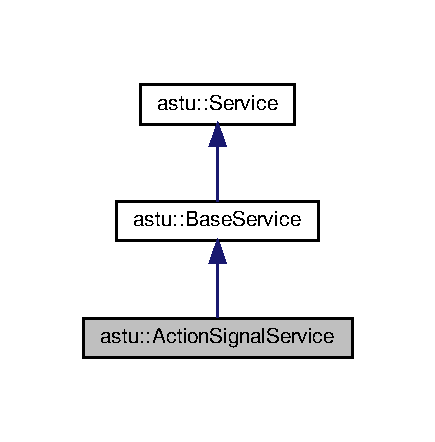
\includegraphics[width=209pt]{classastu_1_1ActionSignalService__inherit__graph}
\end{center}
\end{figure}


Collaboration diagram for astu\+:\+:Action\+Signal\+Service\+:\nopagebreak
\begin{figure}[H]
\begin{center}
\leavevmode
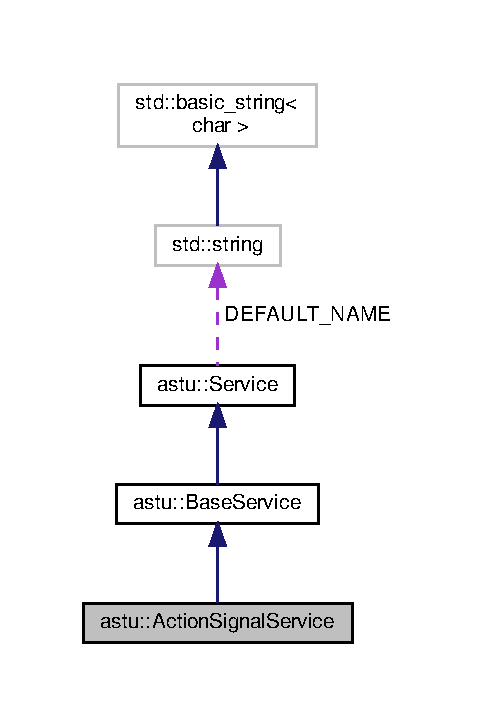
\includegraphics[width=229pt]{classastu_1_1ActionSignalService__coll__graph}
\end{center}
\end{figure}
\subsection*{Public Member Functions}
\begin{DoxyCompactItemize}
\item 
\hyperlink{classastu_1_1ActionSignalService_ad37b42544d39ddbca48668e18c4055d8}{Action\+Signal\+Service} ()
\item 
void \hyperlink{classastu_1_1ActionSignalService_a21b2cca24b3835063b4bf1d59157ab80}{Add\+Signal} (const std\+::string \&action, const std\+::string \&signal)
\item 
void \hyperlink{classastu_1_1ActionSignalService_ae9e72c9808b02e9dbdb6ad164a535514}{Remove\+Signal} (const std\+::string \&action, const std\+::string \&signal)
\end{DoxyCompactItemize}
\subsection*{Additional Inherited Members}


\subsection{Detailed Description}
This service receives actions and converts them into signals. 

\subsection{Constructor \& Destructor Documentation}
\mbox{\Hypertarget{classastu_1_1ActionSignalService_ad37b42544d39ddbca48668e18c4055d8}\label{classastu_1_1ActionSignalService_ad37b42544d39ddbca48668e18c4055d8}} 
\index{astu\+::\+Action\+Signal\+Service@{astu\+::\+Action\+Signal\+Service}!Action\+Signal\+Service@{Action\+Signal\+Service}}
\index{Action\+Signal\+Service@{Action\+Signal\+Service}!astu\+::\+Action\+Signal\+Service@{astu\+::\+Action\+Signal\+Service}}
\subsubsection{\texorpdfstring{Action\+Signal\+Service()}{ActionSignalService()}}
{\footnotesize\ttfamily astu\+::\+Action\+Signal\+Service\+::\+Action\+Signal\+Service (\begin{DoxyParamCaption}{ }\end{DoxyParamCaption})}

Constructor. 

\subsection{Member Function Documentation}
\mbox{\Hypertarget{classastu_1_1ActionSignalService_a21b2cca24b3835063b4bf1d59157ab80}\label{classastu_1_1ActionSignalService_a21b2cca24b3835063b4bf1d59157ab80}} 
\index{astu\+::\+Action\+Signal\+Service@{astu\+::\+Action\+Signal\+Service}!Add\+Signal@{Add\+Signal}}
\index{Add\+Signal@{Add\+Signal}!astu\+::\+Action\+Signal\+Service@{astu\+::\+Action\+Signal\+Service}}
\subsubsection{\texorpdfstring{Add\+Signal()}{AddSignal()}}
{\footnotesize\ttfamily void astu\+::\+Action\+Signal\+Service\+::\+Add\+Signal (\begin{DoxyParamCaption}\item[{const std\+::string \&}]{action,  }\item[{const std\+::string \&}]{signal }\end{DoxyParamCaption})}

Adds a signal to be sent when a certain action is triggered.


\begin{DoxyParams}{Parameters}
{\em action} & the action that triggers the signal \\
\hline
{\em signal} & the signal to be sent \\
\hline
\end{DoxyParams}
\mbox{\Hypertarget{classastu_1_1ActionSignalService_ae9e72c9808b02e9dbdb6ad164a535514}\label{classastu_1_1ActionSignalService_ae9e72c9808b02e9dbdb6ad164a535514}} 
\index{astu\+::\+Action\+Signal\+Service@{astu\+::\+Action\+Signal\+Service}!Remove\+Signal@{Remove\+Signal}}
\index{Remove\+Signal@{Remove\+Signal}!astu\+::\+Action\+Signal\+Service@{astu\+::\+Action\+Signal\+Service}}
\subsubsection{\texorpdfstring{Remove\+Signal()}{RemoveSignal()}}
{\footnotesize\ttfamily void astu\+::\+Action\+Signal\+Service\+::\+Remove\+Signal (\begin{DoxyParamCaption}\item[{const std\+::string \&}]{action,  }\item[{const std\+::string \&}]{signal }\end{DoxyParamCaption})}

Removes the signal to be sent. 
\begin{DoxyParams}{Parameters}
{\em action} & the action that triggers the signal \\
\hline
{\em signal} & the signal to be sent \\
\hline
\end{DoxyParams}


The documentation for this class was generated from the following file\+:\begin{DoxyCompactItemize}
\item 
include/\+Service/Action\+Signal\+Service.\+h\end{DoxyCompactItemize}

\hypertarget{classastu_1_1Application}{}\section{astu\+:\+:Application Class Reference}
\label{classastu_1_1Application}\index{astu\+::\+Application@{astu\+::\+Application}}


{\ttfamily \#include $<$Application.\+h$>$}

\subsection*{Public Member Functions}
\begin{DoxyCompactItemize}
\item 
\hyperlink{classastu_1_1Application_a8fd6025d4412ece9dc752a4a988f833f}{Application} ()
\item 
virtual \hyperlink{classastu_1_1Application_a9f165c3c8eba9eb7e09949aab426d653}{$\sim$\+Application} ()
\item 
void \hyperlink{classastu_1_1Application_a6d991cdd5263dd9d1a08218c84e70a24}{Set\+Width} (int w)
\item 
void \hyperlink{classastu_1_1Application_a192e4c7ccec81846119762f30aceaf12}{Set\+Height} (int h)
\item 
int \hyperlink{classastu_1_1Application_af6f316ed892f9bf487d49d5ba1309e3f}{Get\+Width} () const
\item 
int \hyperlink{classastu_1_1Application_aacee0ec39dbde4c506987abe4be99099}{Get\+Height} () const
\item 
void \hyperlink{classastu_1_1Application_ab1563999702c9d6ae6e707c4cd2c80c6}{Set\+Background\+Color} (const \hyperlink{classastu_1_1Color}{Color4d} \&c)
\item 
\hyperlink{classastu_1_1Color}{Color4d} \hyperlink{classastu_1_1Application_ab033ca3bac5e8423638c118e5f92c62b}{Get\+Background\+Color} () const
\item 
void \hyperlink{classastu_1_1Application_aa311d33c9784e7326a9633336176fe05}{Set\+Draw\+Color} (const \hyperlink{classastu_1_1Color}{Color4d} \&c)
\item 
\hyperlink{classastu_1_1Color}{Color4d} \hyperlink{classastu_1_1Application_a0b019c1dc5797d4ee5e604ed5cd831ed}{Get\+Draw\+Color} () const
\item 
void \hyperlink{classastu_1_1Application_afd2e771d8bfd2b1a55e11f62c099078a}{Draw\+Rectangle} (int x, int y, int w, int h, bool filled=true)
\item 
void \hyperlink{classastu_1_1Application_ade2136cdf7123cade44d9f8701018878}{Draw\+Line} (int x1, int y1, int x2, int y2)
\item 
void \hyperlink{classastu_1_1Application_af26daac7b639690cd2682b2b33b77218}{Draw\+Pixel} (int x, int y)
\item 
void \hyperlink{classastu_1_1Application_ae9d3de234f6abde882816e9866bd07bc}{Clear} ()
\item 
void \hyperlink{classastu_1_1Application_a497dd50375ba6694479e0c57c8e32ffd}{Run} ()
\item 
double \hyperlink{classastu_1_1Application_a54815b8eb1210d2a4da6f3f439741a4d}{Get\+Delta\+Time} () const
\item 
double \hyperlink{classastu_1_1Application_afd91358b09a41d418bc1776befdb0fd7}{Get\+Time} () const
\item 
void \hyperlink{classastu_1_1Application_a823b362755043240ba83b785038720ac}{Reset\+Time} (double t=0)
\item 
double \hyperlink{classastu_1_1Application_a500d7e7a9c0100b8a4e1df2f80f85da9}{Get\+Fps} () const
\item 
void \hyperlink{classastu_1_1Application_aa5336d4fa0fff6231b4260888cb04440}{Set\+Title} (const std\+::string \&title)
\item 
std\+::string \hyperlink{classastu_1_1Application_a7456b7ba3af6c3d984d6f4e40b268426}{Get\+Title} () const
\end{DoxyCompactItemize}
\subsection*{Protected Member Functions}
\begin{DoxyCompactItemize}
\item 
virtual void \hyperlink{classastu_1_1Application_ae7eb0ef242caceca38890f78ddb85718}{On\+Render} ()
\item 
virtual void \hyperlink{classastu_1_1Application_a337064e8db0320f0ffe23ed98fc9fd85}{On\+Startup} ()
\item 
virtual void \hyperlink{classastu_1_1Application_a1894a6f4aca54dd7a4c063b614832f3e}{On\+Shutdown} ()
\end{DoxyCompactItemize}


\subsection{Detailed Description}
S\+D\+L-\/based applications can be developed with the help of this class. This implementation represents an intermediate step between A\+S\+T-\/\+Utilities A\+PI Level 0 and Full-\/\+A\+PI. 

\subsection{Constructor \& Destructor Documentation}
\mbox{\Hypertarget{classastu_1_1Application_a8fd6025d4412ece9dc752a4a988f833f}\label{classastu_1_1Application_a8fd6025d4412ece9dc752a4a988f833f}} 
\index{astu\+::\+Application@{astu\+::\+Application}!Application@{Application}}
\index{Application@{Application}!astu\+::\+Application@{astu\+::\+Application}}
\subsubsection{\texorpdfstring{Application()}{Application()}}
{\footnotesize\ttfamily astu\+::\+Application\+::\+Application (\begin{DoxyParamCaption}{ }\end{DoxyParamCaption})}

Constructor. \mbox{\Hypertarget{classastu_1_1Application_a9f165c3c8eba9eb7e09949aab426d653}\label{classastu_1_1Application_a9f165c3c8eba9eb7e09949aab426d653}} 
\index{astu\+::\+Application@{astu\+::\+Application}!````~Application@{$\sim$\+Application}}
\index{````~Application@{$\sim$\+Application}!astu\+::\+Application@{astu\+::\+Application}}
\subsubsection{\texorpdfstring{$\sim$\+Application()}{~Application()}}
{\footnotesize\ttfamily virtual astu\+::\+Application\+::$\sim$\+Application (\begin{DoxyParamCaption}{ }\end{DoxyParamCaption})\hspace{0.3cm}{\ttfamily [virtual]}}

Virtual destructor. 

\subsection{Member Function Documentation}
\mbox{\Hypertarget{classastu_1_1Application_ae9d3de234f6abde882816e9866bd07bc}\label{classastu_1_1Application_ae9d3de234f6abde882816e9866bd07bc}} 
\index{astu\+::\+Application@{astu\+::\+Application}!Clear@{Clear}}
\index{Clear@{Clear}!astu\+::\+Application@{astu\+::\+Application}}
\subsubsection{\texorpdfstring{Clear()}{Clear()}}
{\footnotesize\ttfamily void astu\+::\+Application\+::\+Clear (\begin{DoxyParamCaption}{ }\end{DoxyParamCaption})}

Clears the canvas using the current clear color. \mbox{\Hypertarget{classastu_1_1Application_ade2136cdf7123cade44d9f8701018878}\label{classastu_1_1Application_ade2136cdf7123cade44d9f8701018878}} 
\index{astu\+::\+Application@{astu\+::\+Application}!Draw\+Line@{Draw\+Line}}
\index{Draw\+Line@{Draw\+Line}!astu\+::\+Application@{astu\+::\+Application}}
\subsubsection{\texorpdfstring{Draw\+Line()}{DrawLine()}}
{\footnotesize\ttfamily void astu\+::\+Application\+::\+Draw\+Line (\begin{DoxyParamCaption}\item[{int}]{x1,  }\item[{int}]{y1,  }\item[{int}]{x2,  }\item[{int}]{y2 }\end{DoxyParamCaption})}

Draws a line with the current draw color.


\begin{DoxyParams}{Parameters}
{\em x1} & the x-\/coordinate of the start point \\
\hline
{\em y1} & the y-\/coordinate of the start point \\
\hline
{\em x2} & the x-\/coordinate of the end point \\
\hline
{\em y2} & the y-\/coordinate of the end point \\
\hline
\end{DoxyParams}
\mbox{\Hypertarget{classastu_1_1Application_af26daac7b639690cd2682b2b33b77218}\label{classastu_1_1Application_af26daac7b639690cd2682b2b33b77218}} 
\index{astu\+::\+Application@{astu\+::\+Application}!Draw\+Pixel@{Draw\+Pixel}}
\index{Draw\+Pixel@{Draw\+Pixel}!astu\+::\+Application@{astu\+::\+Application}}
\subsubsection{\texorpdfstring{Draw\+Pixel()}{DrawPixel()}}
{\footnotesize\ttfamily void astu\+::\+Application\+::\+Draw\+Pixel (\begin{DoxyParamCaption}\item[{int}]{x,  }\item[{int}]{y }\end{DoxyParamCaption})}

Draws a pixel with the current draw color.


\begin{DoxyParams}{Parameters}
{\em x} & the x-\/coordinate of the start point \\
\hline
{\em y} & the y-\/coordinate of the start point \\
\hline
\end{DoxyParams}
\mbox{\Hypertarget{classastu_1_1Application_afd2e771d8bfd2b1a55e11f62c099078a}\label{classastu_1_1Application_afd2e771d8bfd2b1a55e11f62c099078a}} 
\index{astu\+::\+Application@{astu\+::\+Application}!Draw\+Rectangle@{Draw\+Rectangle}}
\index{Draw\+Rectangle@{Draw\+Rectangle}!astu\+::\+Application@{astu\+::\+Application}}
\subsubsection{\texorpdfstring{Draw\+Rectangle()}{DrawRectangle()}}
{\footnotesize\ttfamily void astu\+::\+Application\+::\+Draw\+Rectangle (\begin{DoxyParamCaption}\item[{int}]{x,  }\item[{int}]{y,  }\item[{int}]{w,  }\item[{int}]{h,  }\item[{bool}]{filled = {\ttfamily true} }\end{DoxyParamCaption})}

Draws a rectangle with the current draw color.


\begin{DoxyParams}{Parameters}
{\em x} & the x location of the upper left corner \\
\hline
{\em y} & the y location of the upper left corner \\
\hline
{\em w} & the width of the rectangle \\
\hline
{\em h} & the height of the rectangle \\
\hline
{\em filled} & {\ttfamily true} to render the rectangle filled \\
\hline
\end{DoxyParams}
\mbox{\Hypertarget{classastu_1_1Application_ab033ca3bac5e8423638c118e5f92c62b}\label{classastu_1_1Application_ab033ca3bac5e8423638c118e5f92c62b}} 
\index{astu\+::\+Application@{astu\+::\+Application}!Get\+Background\+Color@{Get\+Background\+Color}}
\index{Get\+Background\+Color@{Get\+Background\+Color}!astu\+::\+Application@{astu\+::\+Application}}
\subsubsection{\texorpdfstring{Get\+Background\+Color()}{GetBackgroundColor()}}
{\footnotesize\ttfamily \hyperlink{classastu_1_1Color}{Color4d} astu\+::\+Application\+::\+Get\+Background\+Color (\begin{DoxyParamCaption}{ }\end{DoxyParamCaption}) const}

Returns the background color for the application window.

\begin{DoxyReturn}{Returns}
the current background color 
\end{DoxyReturn}
\mbox{\Hypertarget{classastu_1_1Application_a54815b8eb1210d2a4da6f3f439741a4d}\label{classastu_1_1Application_a54815b8eb1210d2a4da6f3f439741a4d}} 
\index{astu\+::\+Application@{astu\+::\+Application}!Get\+Delta\+Time@{Get\+Delta\+Time}}
\index{Get\+Delta\+Time@{Get\+Delta\+Time}!astu\+::\+Application@{astu\+::\+Application}}
\subsubsection{\texorpdfstring{Get\+Delta\+Time()}{GetDeltaTime()}}
{\footnotesize\ttfamily double astu\+::\+Application\+::\+Get\+Delta\+Time (\begin{DoxyParamCaption}{ }\end{DoxyParamCaption}) const}

Returns the elapsed time since the last update.

\begin{DoxyReturn}{Returns}
the elapsed time in seconds 
\end{DoxyReturn}
\mbox{\Hypertarget{classastu_1_1Application_a0b019c1dc5797d4ee5e604ed5cd831ed}\label{classastu_1_1Application_a0b019c1dc5797d4ee5e604ed5cd831ed}} 
\index{astu\+::\+Application@{astu\+::\+Application}!Get\+Draw\+Color@{Get\+Draw\+Color}}
\index{Get\+Draw\+Color@{Get\+Draw\+Color}!astu\+::\+Application@{astu\+::\+Application}}
\subsubsection{\texorpdfstring{Get\+Draw\+Color()}{GetDrawColor()}}
{\footnotesize\ttfamily \hyperlink{classastu_1_1Color}{Color4d} astu\+::\+Application\+::\+Get\+Draw\+Color (\begin{DoxyParamCaption}{ }\end{DoxyParamCaption}) const}

Returns the draw color for the application window.

\begin{DoxyReturn}{Returns}
the current draw color 
\end{DoxyReturn}
\mbox{\Hypertarget{classastu_1_1Application_a500d7e7a9c0100b8a4e1df2f80f85da9}\label{classastu_1_1Application_a500d7e7a9c0100b8a4e1df2f80f85da9}} 
\index{astu\+::\+Application@{astu\+::\+Application}!Get\+Fps@{Get\+Fps}}
\index{Get\+Fps@{Get\+Fps}!astu\+::\+Application@{astu\+::\+Application}}
\subsubsection{\texorpdfstring{Get\+Fps()}{GetFps()}}
{\footnotesize\ttfamily double astu\+::\+Application\+::\+Get\+Fps (\begin{DoxyParamCaption}{ }\end{DoxyParamCaption}) const}

Returns the average frames per seconds (F\+PS).

\begin{DoxyReturn}{Returns}
the F\+PS in seconds 
\end{DoxyReturn}
\mbox{\Hypertarget{classastu_1_1Application_aacee0ec39dbde4c506987abe4be99099}\label{classastu_1_1Application_aacee0ec39dbde4c506987abe4be99099}} 
\index{astu\+::\+Application@{astu\+::\+Application}!Get\+Height@{Get\+Height}}
\index{Get\+Height@{Get\+Height}!astu\+::\+Application@{astu\+::\+Application}}
\subsubsection{\texorpdfstring{Get\+Height()}{GetHeight()}}
{\footnotesize\ttfamily int astu\+::\+Application\+::\+Get\+Height (\begin{DoxyParamCaption}{ }\end{DoxyParamCaption}) const}

Returns the width of the application window.

\begin{DoxyReturn}{Returns}
the height in pixels 
\end{DoxyReturn}
\mbox{\Hypertarget{classastu_1_1Application_afd91358b09a41d418bc1776befdb0fd7}\label{classastu_1_1Application_afd91358b09a41d418bc1776befdb0fd7}} 
\index{astu\+::\+Application@{astu\+::\+Application}!Get\+Time@{Get\+Time}}
\index{Get\+Time@{Get\+Time}!astu\+::\+Application@{astu\+::\+Application}}
\subsubsection{\texorpdfstring{Get\+Time()}{GetTime()}}
{\footnotesize\ttfamily double astu\+::\+Application\+::\+Get\+Time (\begin{DoxyParamCaption}{ }\end{DoxyParamCaption}) const}

Returns the absolute time.

\begin{DoxyReturn}{Returns}
the absolute time in seconds. 
\end{DoxyReturn}
\mbox{\Hypertarget{classastu_1_1Application_a7456b7ba3af6c3d984d6f4e40b268426}\label{classastu_1_1Application_a7456b7ba3af6c3d984d6f4e40b268426}} 
\index{astu\+::\+Application@{astu\+::\+Application}!Get\+Title@{Get\+Title}}
\index{Get\+Title@{Get\+Title}!astu\+::\+Application@{astu\+::\+Application}}
\subsubsection{\texorpdfstring{Get\+Title()}{GetTitle()}}
{\footnotesize\ttfamily std\+::string astu\+::\+Application\+::\+Get\+Title (\begin{DoxyParamCaption}{ }\end{DoxyParamCaption}) const}

Returns the title of the application window.

\begin{DoxyReturn}{Returns}
the title of the application window 
\end{DoxyReturn}
\mbox{\Hypertarget{classastu_1_1Application_af6f316ed892f9bf487d49d5ba1309e3f}\label{classastu_1_1Application_af6f316ed892f9bf487d49d5ba1309e3f}} 
\index{astu\+::\+Application@{astu\+::\+Application}!Get\+Width@{Get\+Width}}
\index{Get\+Width@{Get\+Width}!astu\+::\+Application@{astu\+::\+Application}}
\subsubsection{\texorpdfstring{Get\+Width()}{GetWidth()}}
{\footnotesize\ttfamily int astu\+::\+Application\+::\+Get\+Width (\begin{DoxyParamCaption}{ }\end{DoxyParamCaption}) const}

Returns the width of the application window.

\begin{DoxyReturn}{Returns}
the width in pixels 
\end{DoxyReturn}
\mbox{\Hypertarget{classastu_1_1Application_ae7eb0ef242caceca38890f78ddb85718}\label{classastu_1_1Application_ae7eb0ef242caceca38890f78ddb85718}} 
\index{astu\+::\+Application@{astu\+::\+Application}!On\+Render@{On\+Render}}
\index{On\+Render@{On\+Render}!astu\+::\+Application@{astu\+::\+Application}}
\subsubsection{\texorpdfstring{On\+Render()}{OnRender()}}
{\footnotesize\ttfamily virtual void astu\+::\+Application\+::\+On\+Render (\begin{DoxyParamCaption}{ }\end{DoxyParamCaption})\hspace{0.3cm}{\ttfamily [inline]}, {\ttfamily [protected]}, {\ttfamily [virtual]}}

Called by this base class to render application specific content. \mbox{\Hypertarget{classastu_1_1Application_a1894a6f4aca54dd7a4c063b614832f3e}\label{classastu_1_1Application_a1894a6f4aca54dd7a4c063b614832f3e}} 
\index{astu\+::\+Application@{astu\+::\+Application}!On\+Shutdown@{On\+Shutdown}}
\index{On\+Shutdown@{On\+Shutdown}!astu\+::\+Application@{astu\+::\+Application}}
\subsubsection{\texorpdfstring{On\+Shutdown()}{OnShutdown()}}
{\footnotesize\ttfamily virtual void astu\+::\+Application\+::\+On\+Shutdown (\begin{DoxyParamCaption}{ }\end{DoxyParamCaption})\hspace{0.3cm}{\ttfamily [inline]}, {\ttfamily [protected]}, {\ttfamily [virtual]}}

Called by this base class when the application is shutdown. \mbox{\Hypertarget{classastu_1_1Application_a337064e8db0320f0ffe23ed98fc9fd85}\label{classastu_1_1Application_a337064e8db0320f0ffe23ed98fc9fd85}} 
\index{astu\+::\+Application@{astu\+::\+Application}!On\+Startup@{On\+Startup}}
\index{On\+Startup@{On\+Startup}!astu\+::\+Application@{astu\+::\+Application}}
\subsubsection{\texorpdfstring{On\+Startup()}{OnStartup()}}
{\footnotesize\ttfamily virtual void astu\+::\+Application\+::\+On\+Startup (\begin{DoxyParamCaption}{ }\end{DoxyParamCaption})\hspace{0.3cm}{\ttfamily [inline]}, {\ttfamily [protected]}, {\ttfamily [virtual]}}

Called by this base class when the application is started. \mbox{\Hypertarget{classastu_1_1Application_a823b362755043240ba83b785038720ac}\label{classastu_1_1Application_a823b362755043240ba83b785038720ac}} 
\index{astu\+::\+Application@{astu\+::\+Application}!Reset\+Time@{Reset\+Time}}
\index{Reset\+Time@{Reset\+Time}!astu\+::\+Application@{astu\+::\+Application}}
\subsubsection{\texorpdfstring{Reset\+Time()}{ResetTime()}}
{\footnotesize\ttfamily void astu\+::\+Application\+::\+Reset\+Time (\begin{DoxyParamCaption}\item[{double}]{t = {\ttfamily 0} }\end{DoxyParamCaption})}

Resets the absolute time to the specified value.


\begin{DoxyParams}{Parameters}
{\em t} & the absolute time in seconds \\
\hline
\end{DoxyParams}
\mbox{\Hypertarget{classastu_1_1Application_a497dd50375ba6694479e0c57c8e32ffd}\label{classastu_1_1Application_a497dd50375ba6694479e0c57c8e32ffd}} 
\index{astu\+::\+Application@{astu\+::\+Application}!Run@{Run}}
\index{Run@{Run}!astu\+::\+Application@{astu\+::\+Application}}
\subsubsection{\texorpdfstring{Run()}{Run()}}
{\footnotesize\ttfamily void astu\+::\+Application\+::\+Run (\begin{DoxyParamCaption}{ }\end{DoxyParamCaption})}

Starts this application. \mbox{\Hypertarget{classastu_1_1Application_ab1563999702c9d6ae6e707c4cd2c80c6}\label{classastu_1_1Application_ab1563999702c9d6ae6e707c4cd2c80c6}} 
\index{astu\+::\+Application@{astu\+::\+Application}!Set\+Background\+Color@{Set\+Background\+Color}}
\index{Set\+Background\+Color@{Set\+Background\+Color}!astu\+::\+Application@{astu\+::\+Application}}
\subsubsection{\texorpdfstring{Set\+Background\+Color()}{SetBackgroundColor()}}
{\footnotesize\ttfamily void astu\+::\+Application\+::\+Set\+Background\+Color (\begin{DoxyParamCaption}\item[{const \hyperlink{classastu_1_1Color}{Color4d} \&}]{c }\end{DoxyParamCaption})}

Sets the background color of the application window.


\begin{DoxyParams}{Parameters}
{\em c} & the background color \\
\hline
\end{DoxyParams}
\mbox{\Hypertarget{classastu_1_1Application_aa311d33c9784e7326a9633336176fe05}\label{classastu_1_1Application_aa311d33c9784e7326a9633336176fe05}} 
\index{astu\+::\+Application@{astu\+::\+Application}!Set\+Draw\+Color@{Set\+Draw\+Color}}
\index{Set\+Draw\+Color@{Set\+Draw\+Color}!astu\+::\+Application@{astu\+::\+Application}}
\subsubsection{\texorpdfstring{Set\+Draw\+Color()}{SetDrawColor()}}
{\footnotesize\ttfamily void astu\+::\+Application\+::\+Set\+Draw\+Color (\begin{DoxyParamCaption}\item[{const \hyperlink{classastu_1_1Color}{Color4d} \&}]{c }\end{DoxyParamCaption})}

Sets the draw color of the application window.


\begin{DoxyParams}{Parameters}
{\em c} & the draw color \\
\hline
\end{DoxyParams}
\mbox{\Hypertarget{classastu_1_1Application_a192e4c7ccec81846119762f30aceaf12}\label{classastu_1_1Application_a192e4c7ccec81846119762f30aceaf12}} 
\index{astu\+::\+Application@{astu\+::\+Application}!Set\+Height@{Set\+Height}}
\index{Set\+Height@{Set\+Height}!astu\+::\+Application@{astu\+::\+Application}}
\subsubsection{\texorpdfstring{Set\+Height()}{SetHeight()}}
{\footnotesize\ttfamily void astu\+::\+Application\+::\+Set\+Height (\begin{DoxyParamCaption}\item[{int}]{h }\end{DoxyParamCaption})}

Sets the height of the application window.


\begin{DoxyParams}{Parameters}
{\em h} & the height in pixels \\
\hline
\end{DoxyParams}
\mbox{\Hypertarget{classastu_1_1Application_aa5336d4fa0fff6231b4260888cb04440}\label{classastu_1_1Application_aa5336d4fa0fff6231b4260888cb04440}} 
\index{astu\+::\+Application@{astu\+::\+Application}!Set\+Title@{Set\+Title}}
\index{Set\+Title@{Set\+Title}!astu\+::\+Application@{astu\+::\+Application}}
\subsubsection{\texorpdfstring{Set\+Title()}{SetTitle()}}
{\footnotesize\ttfamily void astu\+::\+Application\+::\+Set\+Title (\begin{DoxyParamCaption}\item[{const std\+::string \&}]{title }\end{DoxyParamCaption})}

Sets the title of the application window.


\begin{DoxyParams}{Parameters}
{\em title} & the title of the window \\
\hline
\end{DoxyParams}
\mbox{\Hypertarget{classastu_1_1Application_a6d991cdd5263dd9d1a08218c84e70a24}\label{classastu_1_1Application_a6d991cdd5263dd9d1a08218c84e70a24}} 
\index{astu\+::\+Application@{astu\+::\+Application}!Set\+Width@{Set\+Width}}
\index{Set\+Width@{Set\+Width}!astu\+::\+Application@{astu\+::\+Application}}
\subsubsection{\texorpdfstring{Set\+Width()}{SetWidth()}}
{\footnotesize\ttfamily void astu\+::\+Application\+::\+Set\+Width (\begin{DoxyParamCaption}\item[{int}]{w }\end{DoxyParamCaption})}

Sets the width of the application window.


\begin{DoxyParams}{Parameters}
{\em w} & the width in pixels \\
\hline
\end{DoxyParams}


The documentation for this class was generated from the following file\+:\begin{DoxyCompactItemize}
\item 
include/\+Suite\+S\+D\+L/Application.\+h\end{DoxyCompactItemize}

\hypertarget{classastu_1_1AutoDestructSystem}{}\section{astu\+:\+:Auto\+Destruct\+System Class Reference}
\label{classastu_1_1AutoDestructSystem}\index{astu\+::\+Auto\+Destruct\+System@{astu\+::\+Auto\+Destruct\+System}}


{\ttfamily \#include $<$Auto\+Destruct\+System.\+h$>$}



Inheritance diagram for astu\+:\+:Auto\+Destruct\+System\+:
\nopagebreak
\begin{figure}[H]
\begin{center}
\leavevmode
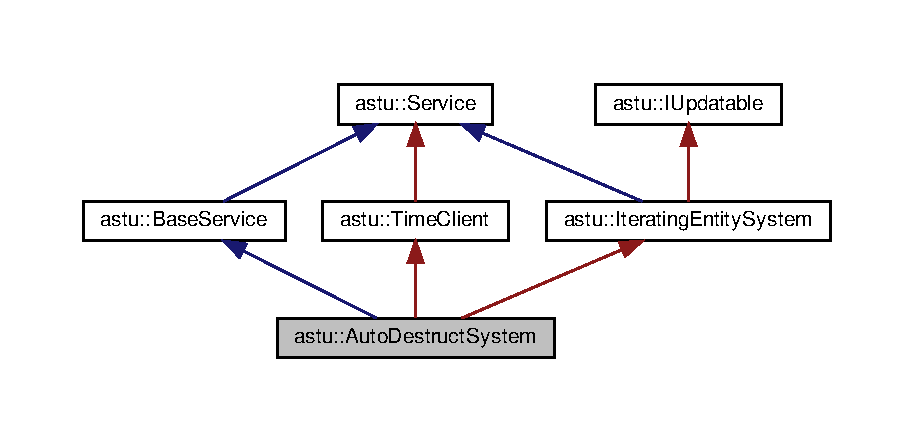
\includegraphics[width=350pt]{classastu_1_1AutoDestructSystem__inherit__graph}
\end{center}
\end{figure}


Collaboration diagram for astu\+:\+:Auto\+Destruct\+System\+:
\nopagebreak
\begin{figure}[H]
\begin{center}
\leavevmode
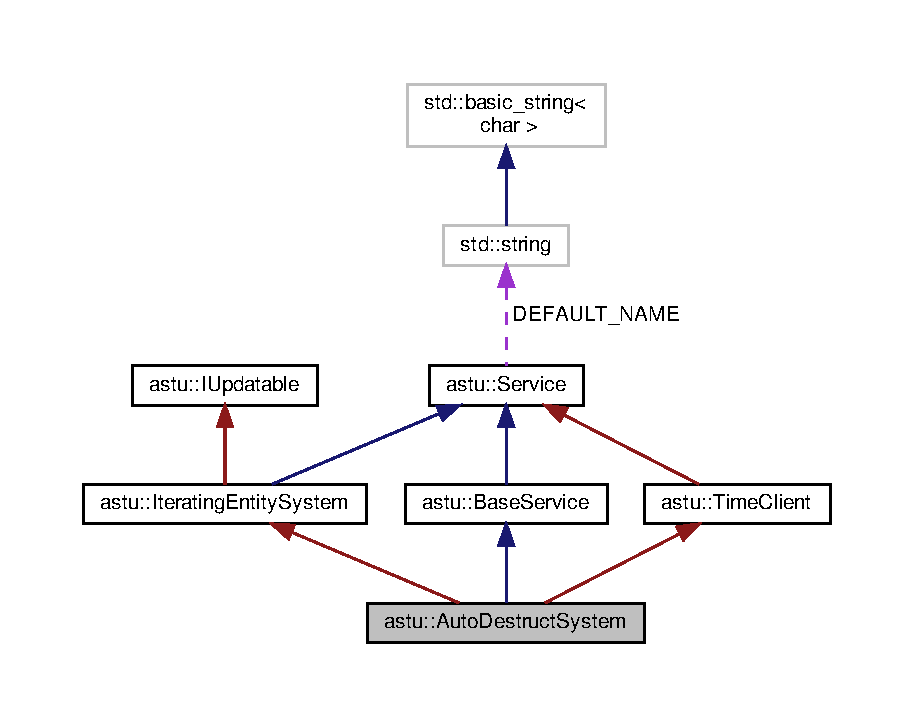
\includegraphics[width=350pt]{classastu_1_1AutoDestructSystem__coll__graph}
\end{center}
\end{figure}
\subsection*{Public Member Functions}
\begin{DoxyCompactItemize}
\item 
\hyperlink{classastu_1_1AutoDestructSystem_a01cf2ca0427902e70bc2767cbc00b447}{Auto\+Destruct\+System} (int update\+Priority=astu\+::\+Priority\+::\+Normal)
\end{DoxyCompactItemize}
\subsection*{Additional Inherited Members}


\subsection{Detailed Description}
This entity system removes entities after a certain amount of time.

This system relies on C\+Pose and \hyperlink{classastu_1_1CAutoDestruct}{C\+Auto\+Destruct} components. 

\subsection{Constructor \& Destructor Documentation}
\mbox{\Hypertarget{classastu_1_1AutoDestructSystem_a01cf2ca0427902e70bc2767cbc00b447}\label{classastu_1_1AutoDestructSystem_a01cf2ca0427902e70bc2767cbc00b447}} 
\index{astu\+::\+Auto\+Destruct\+System@{astu\+::\+Auto\+Destruct\+System}!Auto\+Destruct\+System@{Auto\+Destruct\+System}}
\index{Auto\+Destruct\+System@{Auto\+Destruct\+System}!astu\+::\+Auto\+Destruct\+System@{astu\+::\+Auto\+Destruct\+System}}
\subsubsection{\texorpdfstring{Auto\+Destruct\+System()}{AutoDestructSystem()}}
{\footnotesize\ttfamily astu\+::\+Auto\+Destruct\+System\+::\+Auto\+Destruct\+System (\begin{DoxyParamCaption}\item[{int}]{update\+Priority = {\ttfamily astu\+:\+:Priority\+:\+:Normal} }\end{DoxyParamCaption})}

Constructor.


\begin{DoxyParams}{Parameters}
{\em update\+Priority} & the priority used to update this system \\
\hline
\end{DoxyParams}


The documentation for this class was generated from the following file\+:\begin{DoxyCompactItemize}
\item 
include/\+E\+C\+S/Auto\+Destruct\+System.\+h\end{DoxyCompactItemize}

\hypertarget{classastu_1_1suite2d_1_1AutoRotateSystem}{}\section{astu\+:\+:suite2d\+:\+:Auto\+Rotate\+System Class Reference}
\label{classastu_1_1suite2d_1_1AutoRotateSystem}\index{astu\+::suite2d\+::\+Auto\+Rotate\+System@{astu\+::suite2d\+::\+Auto\+Rotate\+System}}


{\ttfamily \#include $<$Auto\+Rotate\+System.\+h$>$}



Inheritance diagram for astu\+:\+:suite2d\+:\+:Auto\+Rotate\+System\+:\nopagebreak
\begin{figure}[H]
\begin{center}
\leavevmode
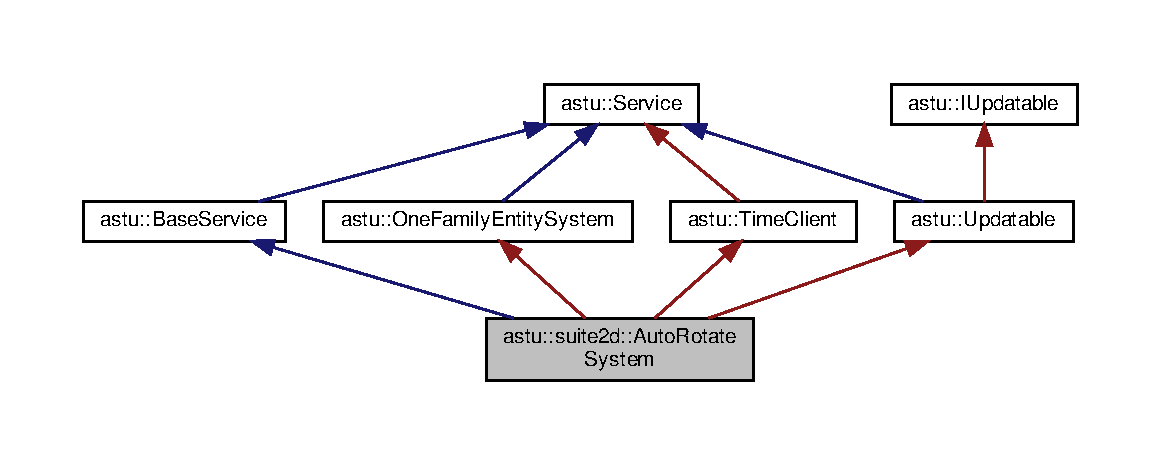
\includegraphics[width=350pt]{classastu_1_1suite2d_1_1AutoRotateSystem__inherit__graph}
\end{center}
\end{figure}


Collaboration diagram for astu\+:\+:suite2d\+:\+:Auto\+Rotate\+System\+:\nopagebreak
\begin{figure}[H]
\begin{center}
\leavevmode
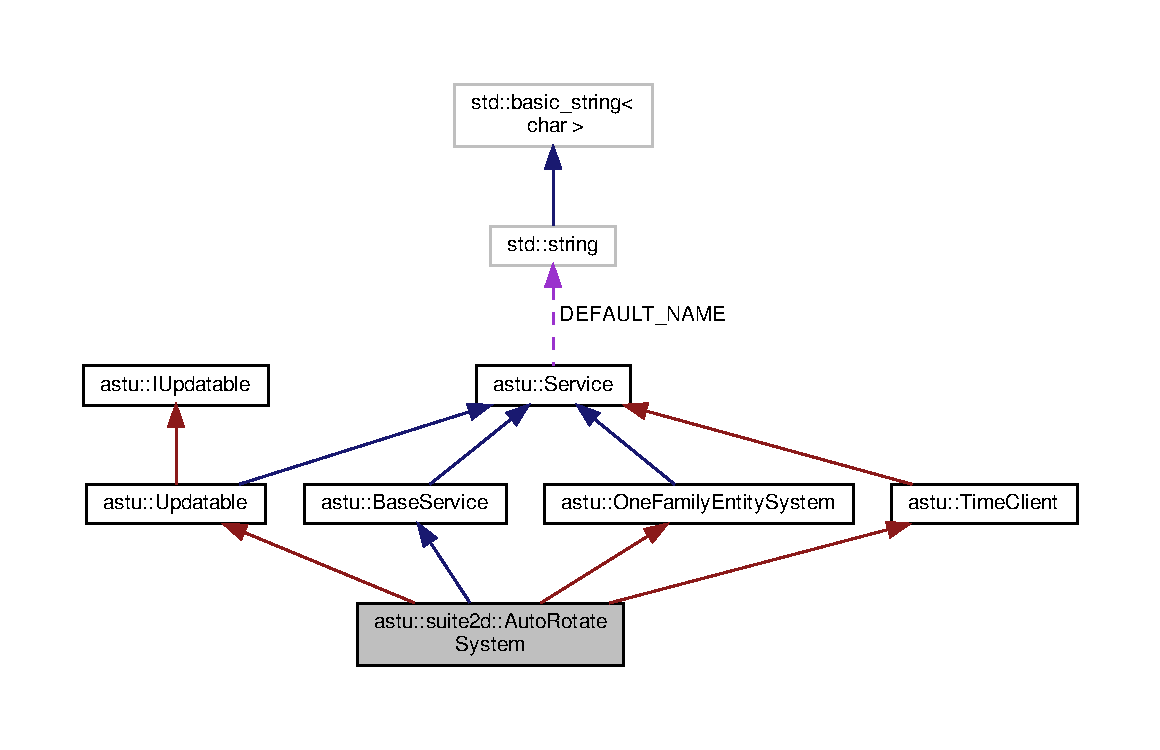
\includegraphics[width=350pt]{classastu_1_1suite2d_1_1AutoRotateSystem__coll__graph}
\end{center}
\end{figure}
\subsection*{Public Member Functions}
\begin{DoxyCompactItemize}
\item 
\hyperlink{classastu_1_1suite2d_1_1AutoRotateSystem_a61d7b59f9cadba07d3a49efd2433e4bc}{Auto\+Rotate\+System} (int update\+Priority=astu\+::\+Priority\+::\+Normal)
\end{DoxyCompactItemize}
\subsection*{Additional Inherited Members}


\subsection{Detailed Description}
This auto-\/rotate system rotates entities with a constant speed. This system relies on \hyperlink{classastu_1_1suite2d_1_1CPose}{C\+Pose} and \hyperlink{classastu_1_1suite2d_1_1CAutoRotate}{C\+Auto\+Rotate} components. 

\subsection{Constructor \& Destructor Documentation}
\mbox{\Hypertarget{classastu_1_1suite2d_1_1AutoRotateSystem_a61d7b59f9cadba07d3a49efd2433e4bc}\label{classastu_1_1suite2d_1_1AutoRotateSystem_a61d7b59f9cadba07d3a49efd2433e4bc}} 
\index{astu\+::suite2d\+::\+Auto\+Rotate\+System@{astu\+::suite2d\+::\+Auto\+Rotate\+System}!Auto\+Rotate\+System@{Auto\+Rotate\+System}}
\index{Auto\+Rotate\+System@{Auto\+Rotate\+System}!astu\+::suite2d\+::\+Auto\+Rotate\+System@{astu\+::suite2d\+::\+Auto\+Rotate\+System}}
\subsubsection{\texorpdfstring{Auto\+Rotate\+System()}{AutoRotateSystem()}}
{\footnotesize\ttfamily astu\+::suite2d\+::\+Auto\+Rotate\+System\+::\+Auto\+Rotate\+System (\begin{DoxyParamCaption}\item[{int}]{update\+Priority = {\ttfamily astu\+:\+:Priority\+:\+:Normal} }\end{DoxyParamCaption})}

Constructor.


\begin{DoxyParams}{Parameters}
{\em update\+Priority} & the priority to update this system \\
\hline
\end{DoxyParams}


The documentation for this class was generated from the following file\+:\begin{DoxyCompactItemize}
\item 
include/\+Suite2\+D/Auto\+Rotate\+System.\+h\end{DoxyCompactItemize}

\hypertarget{classastu_1_1AxisBinding}{}\section{astu\+:\+:Axis\+Binding Class Reference}
\label{classastu_1_1AxisBinding}\index{astu\+::\+Axis\+Binding@{astu\+::\+Axis\+Binding}}


{\ttfamily \#include $<$Input\+Mapping\+Service.\+h$>$}

\subsection*{Public Types}
\begin{DoxyCompactItemize}
\item 
using \hyperlink{classastu_1_1AxisBinding_a38f398d407de503bd52019e244fa9687}{Delegate} = std\+::function$<$ void(\hyperlink{classastu_1_1AxisBinding}{Axis\+Binding} \&)$>$
\end{DoxyCompactItemize}
\subsection*{Public Member Functions}
\begin{DoxyCompactItemize}
\item 
\hyperlink{classastu_1_1AxisBinding_a196fdc402dcf64aa507e6d6b9d3757f9}{Axis\+Binding} (const std\+::string \&axis\+Name)
\item 
float \hyperlink{classastu_1_1AxisBinding_a94ddec4241c656506512c312251374b6}{Get\+Value} () const
\item 
const std\+::string \& \hyperlink{classastu_1_1AxisBinding_acc8029d84009c364c17268af4adf4b59}{Get\+Axis} () const
\item 
void \hyperlink{classastu_1_1AxisBinding_a5e7b784a68d99a9ed6fa652e55ecbad4}{Set\+Delegate} (\hyperlink{classastu_1_1AxisBinding_a38f398d407de503bd52019e244fa9687}{Delegate} delegate)
\end{DoxyCompactItemize}
\subsection*{Friends}
\begin{DoxyCompactItemize}
\item 
\mbox{\Hypertarget{classastu_1_1AxisBinding_a8a886d4dcb7950d2c68f97f528f5ab4c}\label{classastu_1_1AxisBinding_a8a886d4dcb7950d2c68f97f528f5ab4c}} 
class {\bfseries Input\+Mapping\+Service}
\end{DoxyCompactItemize}


\subsection{Detailed Description}
Binds an axis to a delegate. 

\subsection{Member Typedef Documentation}
\mbox{\Hypertarget{classastu_1_1AxisBinding_a38f398d407de503bd52019e244fa9687}\label{classastu_1_1AxisBinding_a38f398d407de503bd52019e244fa9687}} 
\index{astu\+::\+Axis\+Binding@{astu\+::\+Axis\+Binding}!Delegate@{Delegate}}
\index{Delegate@{Delegate}!astu\+::\+Axis\+Binding@{astu\+::\+Axis\+Binding}}
\subsubsection{\texorpdfstring{Delegate}{Delegate}}
{\footnotesize\ttfamily using \hyperlink{classastu_1_1AxisBinding_a38f398d407de503bd52019e244fa9687}{astu\+::\+Axis\+Binding\+::\+Delegate} =  std\+::function$<$void (\hyperlink{classastu_1_1AxisBinding}{Axis\+Binding} \&)$>$}

Type alias for delegate functions. 

\subsection{Constructor \& Destructor Documentation}
\mbox{\Hypertarget{classastu_1_1AxisBinding_a196fdc402dcf64aa507e6d6b9d3757f9}\label{classastu_1_1AxisBinding_a196fdc402dcf64aa507e6d6b9d3757f9}} 
\index{astu\+::\+Axis\+Binding@{astu\+::\+Axis\+Binding}!Axis\+Binding@{Axis\+Binding}}
\index{Axis\+Binding@{Axis\+Binding}!astu\+::\+Axis\+Binding@{astu\+::\+Axis\+Binding}}
\subsubsection{\texorpdfstring{Axis\+Binding()}{AxisBinding()}}
{\footnotesize\ttfamily astu\+::\+Axis\+Binding\+::\+Axis\+Binding (\begin{DoxyParamCaption}\item[{const std\+::string \&}]{axis\+Name }\end{DoxyParamCaption})}

Constructor.


\begin{DoxyParams}{Parameters}
{\em axis\+Name} & the name of the axis to bind \\
\hline
\end{DoxyParams}


\subsection{Member Function Documentation}
\mbox{\Hypertarget{classastu_1_1AxisBinding_acc8029d84009c364c17268af4adf4b59}\label{classastu_1_1AxisBinding_acc8029d84009c364c17268af4adf4b59}} 
\index{astu\+::\+Axis\+Binding@{astu\+::\+Axis\+Binding}!Get\+Axis@{Get\+Axis}}
\index{Get\+Axis@{Get\+Axis}!astu\+::\+Axis\+Binding@{astu\+::\+Axis\+Binding}}
\subsubsection{\texorpdfstring{Get\+Axis()}{GetAxis()}}
{\footnotesize\ttfamily const std\+::string\& astu\+::\+Axis\+Binding\+::\+Get\+Axis (\begin{DoxyParamCaption}{ }\end{DoxyParamCaption}) const}

Returns the name of the axis of this binding.

\begin{DoxyReturn}{Returns}
the axis name 
\end{DoxyReturn}
\mbox{\Hypertarget{classastu_1_1AxisBinding_a94ddec4241c656506512c312251374b6}\label{classastu_1_1AxisBinding_a94ddec4241c656506512c312251374b6}} 
\index{astu\+::\+Axis\+Binding@{astu\+::\+Axis\+Binding}!Get\+Value@{Get\+Value}}
\index{Get\+Value@{Get\+Value}!astu\+::\+Axis\+Binding@{astu\+::\+Axis\+Binding}}
\subsubsection{\texorpdfstring{Get\+Value()}{GetValue()}}
{\footnotesize\ttfamily float astu\+::\+Axis\+Binding\+::\+Get\+Value (\begin{DoxyParamCaption}{ }\end{DoxyParamCaption}) const}

Returns the current value of this axis binding.

\begin{DoxyReturn}{Returns}
the current axis value 
\end{DoxyReturn}
\mbox{\Hypertarget{classastu_1_1AxisBinding_a5e7b784a68d99a9ed6fa652e55ecbad4}\label{classastu_1_1AxisBinding_a5e7b784a68d99a9ed6fa652e55ecbad4}} 
\index{astu\+::\+Axis\+Binding@{astu\+::\+Axis\+Binding}!Set\+Delegate@{Set\+Delegate}}
\index{Set\+Delegate@{Set\+Delegate}!astu\+::\+Axis\+Binding@{astu\+::\+Axis\+Binding}}
\subsubsection{\texorpdfstring{Set\+Delegate()}{SetDelegate()}}
{\footnotesize\ttfamily void astu\+::\+Axis\+Binding\+::\+Set\+Delegate (\begin{DoxyParamCaption}\item[{\hyperlink{classastu_1_1AxisBinding_a38f398d407de503bd52019e244fa9687}{Delegate}}]{delegate }\end{DoxyParamCaption})}

Sets the delegate function to be called on state changes.


\begin{DoxyParams}{Parameters}
{\em delegate} & the the delegate function \\
\hline
\end{DoxyParams}


The documentation for this class was generated from the following file\+:\begin{DoxyCompactItemize}
\item 
include/\+Input/Input\+Mapping\+Service.\+h\end{DoxyCompactItemize}

\hypertarget{classastu_1_1AxisMapping}{}\section{astu\+:\+:Axis\+Mapping Class Reference}
\label{classastu_1_1AxisMapping}\index{astu\+::\+Axis\+Mapping@{astu\+::\+Axis\+Mapping}}


{\ttfamily \#include $<$Input\+Mapping\+Service.\+h$>$}

\subsection*{Public Member Functions}
\begin{DoxyCompactItemize}
\item 
\hyperlink{classastu_1_1AxisMapping_a1145f8432af7cea0bc9db96735386d9f}{Axis\+Mapping} (const std\+::string \&name, const \hyperlink{classastu_1_1Key}{Key} \&key, float scale=1)
\item 
const std\+::string \& \hyperlink{classastu_1_1AxisMapping_a6f58533973272cb6f826960810c70600}{Get\+Name} () const
\item 
const \hyperlink{classastu_1_1Key}{Key} \& \hyperlink{classastu_1_1AxisMapping_ac6168d999aca7d2f7e4b71d29e6de12d}{Get\+Key} () const
\item 
float \hyperlink{classastu_1_1AxisMapping_ad06f6315529e72132e27c97b6ff15378}{Get\+Scale} () const
\end{DoxyCompactItemize}


\subsection{Detailed Description}
Maps an axis to an input control (key. 

\subsection{Constructor \& Destructor Documentation}
\mbox{\Hypertarget{classastu_1_1AxisMapping_a1145f8432af7cea0bc9db96735386d9f}\label{classastu_1_1AxisMapping_a1145f8432af7cea0bc9db96735386d9f}} 
\index{astu\+::\+Axis\+Mapping@{astu\+::\+Axis\+Mapping}!Axis\+Mapping@{Axis\+Mapping}}
\index{Axis\+Mapping@{Axis\+Mapping}!astu\+::\+Axis\+Mapping@{astu\+::\+Axis\+Mapping}}
\subsubsection{\texorpdfstring{Axis\+Mapping()}{AxisMapping()}}
{\footnotesize\ttfamily astu\+::\+Axis\+Mapping\+::\+Axis\+Mapping (\begin{DoxyParamCaption}\item[{const std\+::string \&}]{name,  }\item[{const \hyperlink{classastu_1_1Key}{Key} \&}]{key,  }\item[{float}]{scale = {\ttfamily 1} }\end{DoxyParamCaption})}

Constructor.


\begin{DoxyParams}{Parameters}
{\em name} & the name of this mapping \\
\hline
{\em key} & the key of this mapping \\
\hline
{\em scale} & the multiplier on the axis value \\
\hline
\end{DoxyParams}


\subsection{Member Function Documentation}
\mbox{\Hypertarget{classastu_1_1AxisMapping_ac6168d999aca7d2f7e4b71d29e6de12d}\label{classastu_1_1AxisMapping_ac6168d999aca7d2f7e4b71d29e6de12d}} 
\index{astu\+::\+Axis\+Mapping@{astu\+::\+Axis\+Mapping}!Get\+Key@{Get\+Key}}
\index{Get\+Key@{Get\+Key}!astu\+::\+Axis\+Mapping@{astu\+::\+Axis\+Mapping}}
\subsubsection{\texorpdfstring{Get\+Key()}{GetKey()}}
{\footnotesize\ttfamily const \hyperlink{classastu_1_1Key}{Key}\& astu\+::\+Axis\+Mapping\+::\+Get\+Key (\begin{DoxyParamCaption}{ }\end{DoxyParamCaption}) const}

Return the associated \hyperlink{classastu_1_1Key}{Key} of this mapping.

\begin{DoxyReturn}{Returns}
the key 
\end{DoxyReturn}
\mbox{\Hypertarget{classastu_1_1AxisMapping_a6f58533973272cb6f826960810c70600}\label{classastu_1_1AxisMapping_a6f58533973272cb6f826960810c70600}} 
\index{astu\+::\+Axis\+Mapping@{astu\+::\+Axis\+Mapping}!Get\+Name@{Get\+Name}}
\index{Get\+Name@{Get\+Name}!astu\+::\+Axis\+Mapping@{astu\+::\+Axis\+Mapping}}
\subsubsection{\texorpdfstring{Get\+Name()}{GetName()}}
{\footnotesize\ttfamily const std\+::string\& astu\+::\+Axis\+Mapping\+::\+Get\+Name (\begin{DoxyParamCaption}{ }\end{DoxyParamCaption}) const}

Returns the name of the axis of this mapping.

\begin{DoxyReturn}{Returns}
the axis name 
\end{DoxyReturn}
\mbox{\Hypertarget{classastu_1_1AxisMapping_ad06f6315529e72132e27c97b6ff15378}\label{classastu_1_1AxisMapping_ad06f6315529e72132e27c97b6ff15378}} 
\index{astu\+::\+Axis\+Mapping@{astu\+::\+Axis\+Mapping}!Get\+Scale@{Get\+Scale}}
\index{Get\+Scale@{Get\+Scale}!astu\+::\+Axis\+Mapping@{astu\+::\+Axis\+Mapping}}
\subsubsection{\texorpdfstring{Get\+Scale()}{GetScale()}}
{\footnotesize\ttfamily float astu\+::\+Axis\+Mapping\+::\+Get\+Scale (\begin{DoxyParamCaption}{ }\end{DoxyParamCaption}) const}

Returns the axis multiplier.

\begin{DoxyReturn}{Returns}
multiplier on the axis value 
\end{DoxyReturn}


The documentation for this class was generated from the following file\+:\begin{DoxyCompactItemize}
\item 
include/\+Input/Input\+Mapping\+Service.\+h\end{DoxyCompactItemize}

\hypertarget{classastu_1_1BaseService}{}\section{astu\+:\+:Base\+Service Class Reference}
\label{classastu_1_1BaseService}\index{astu\+::\+Base\+Service@{astu\+::\+Base\+Service}}


{\ttfamily \#include $<$Service.\+h$>$}



Inheritance diagram for astu\+:\+:Base\+Service\+:\nopagebreak
\begin{figure}[H]
\begin{center}
\leavevmode
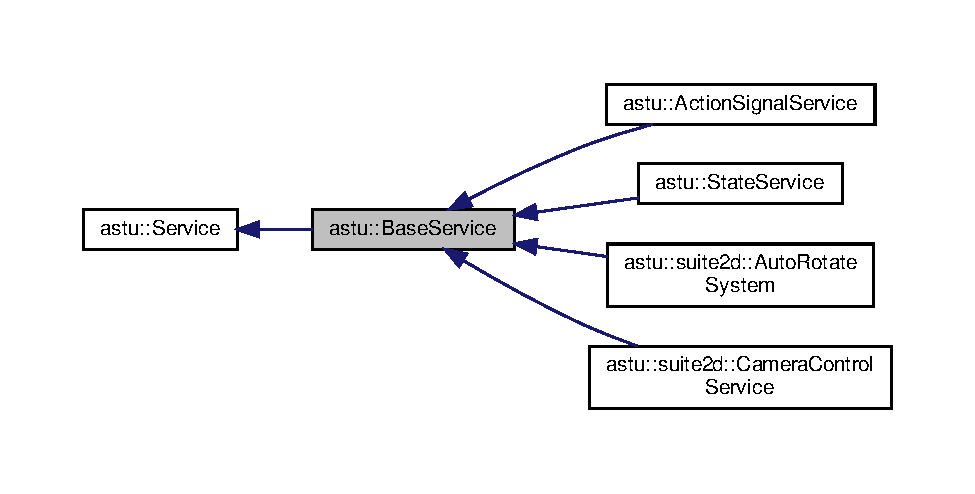
\includegraphics[width=350pt]{classastu_1_1BaseService__inherit__graph}
\end{center}
\end{figure}


Collaboration diagram for astu\+:\+:Base\+Service\+:\nopagebreak
\begin{figure}[H]
\begin{center}
\leavevmode
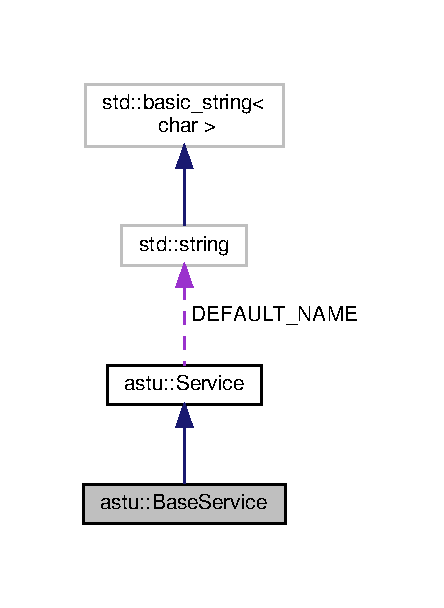
\includegraphics[width=258pt]{classastu_1_1BaseService__coll__graph}
\end{center}
\end{figure}
\subsection*{Public Member Functions}
\begin{DoxyCompactItemize}
\item 
\hyperlink{classastu_1_1BaseService_ab155c73d180c22dab7cf8aff1514b2b5}{Base\+Service} (const std\+::string \&name=\hyperlink{classastu_1_1BaseService_a9483b26ad631bd14646ef2d2170cd828}{D\+E\+F\+A\+U\+L\+T\+\_\+\+N\+A\+ME})
\item 
virtual const std\+::string \& \hyperlink{classastu_1_1BaseService_a42eb6e0d667215ef635682d2a12e1631}{Get\+Name} () const final override
\item 
virtual void \hyperlink{classastu_1_1BaseService_a59dade033dcb44dd32155c526a3a58e2}{Startup} () override
\item 
virtual void \hyperlink{classastu_1_1BaseService_a7095888244052db294d58738c0d187fb}{Shutdown} () override
\item 
virtual bool \hyperlink{classastu_1_1BaseService_af6f4641c045343d329a0fc1ecc6a9778}{Is\+Running} () const override
\end{DoxyCompactItemize}
\subsection*{Static Public Attributes}
\begin{DoxyCompactItemize}
\item 
static const std\+::string \& \hyperlink{classastu_1_1BaseService_a9483b26ad631bd14646ef2d2170cd828}{D\+E\+F\+A\+U\+L\+T\+\_\+\+N\+A\+ME}
\end{DoxyCompactItemize}
\subsection*{Protected Member Functions}
\begin{DoxyCompactItemize}
\item 
virtual void \hyperlink{classastu_1_1BaseService_ac8710cd2d6dcc990db65e7c8ccfbc5ff}{On\+Startup} ()
\item 
virtual void \hyperlink{classastu_1_1BaseService_aeb5003f7c5efe5412725ac4c66942d03}{On\+Shutdown} ()
\item 
\hyperlink{classastu_1_1ServiceManager}{Service\+Manager} \& \hyperlink{classastu_1_1BaseService_a646b6c83a9ebd26fe4e7796b5afde612}{Get\+SM} ()
\end{DoxyCompactItemize}


\subsection{Detailed Description}
Implmenents basic functionality of a service.

This base class can be used to create services with basic functionlality e.\+g, having a name and keeping track if its currently running or not. 

\subsection{Constructor \& Destructor Documentation}
\mbox{\Hypertarget{classastu_1_1BaseService_ab155c73d180c22dab7cf8aff1514b2b5}\label{classastu_1_1BaseService_ab155c73d180c22dab7cf8aff1514b2b5}} 
\index{astu\+::\+Base\+Service@{astu\+::\+Base\+Service}!Base\+Service@{Base\+Service}}
\index{Base\+Service@{Base\+Service}!astu\+::\+Base\+Service@{astu\+::\+Base\+Service}}
\subsubsection{\texorpdfstring{Base\+Service()}{BaseService()}}
{\footnotesize\ttfamily astu\+::\+Base\+Service\+::\+Base\+Service (\begin{DoxyParamCaption}\item[{const std\+::string \&}]{name = {\ttfamily \hyperlink{classastu_1_1BaseService_a9483b26ad631bd14646ef2d2170cd828}{D\+E\+F\+A\+U\+L\+T\+\_\+\+N\+A\+ME}} }\end{DoxyParamCaption})}

Constructor. 

\subsection{Member Function Documentation}
\mbox{\Hypertarget{classastu_1_1BaseService_a42eb6e0d667215ef635682d2a12e1631}\label{classastu_1_1BaseService_a42eb6e0d667215ef635682d2a12e1631}} 
\index{astu\+::\+Base\+Service@{astu\+::\+Base\+Service}!Get\+Name@{Get\+Name}}
\index{Get\+Name@{Get\+Name}!astu\+::\+Base\+Service@{astu\+::\+Base\+Service}}
\subsubsection{\texorpdfstring{Get\+Name()}{GetName()}}
{\footnotesize\ttfamily virtual const std\+::string\& astu\+::\+Base\+Service\+::\+Get\+Name (\begin{DoxyParamCaption}{ }\end{DoxyParamCaption}) const\hspace{0.3cm}{\ttfamily [final]}, {\ttfamily [override]}, {\ttfamily [virtual]}}

Returns the name of this service.

\begin{DoxyReturn}{Returns}
this service\textquotesingle{}s name 
\end{DoxyReturn}


Implements \hyperlink{classastu_1_1IService_a7bfb508c07816c701ceaa72928213380}{astu\+::\+I\+Service}.

\mbox{\Hypertarget{classastu_1_1BaseService_a646b6c83a9ebd26fe4e7796b5afde612}\label{classastu_1_1BaseService_a646b6c83a9ebd26fe4e7796b5afde612}} 
\index{astu\+::\+Base\+Service@{astu\+::\+Base\+Service}!Get\+SM@{Get\+SM}}
\index{Get\+SM@{Get\+SM}!astu\+::\+Base\+Service@{astu\+::\+Base\+Service}}
\subsubsection{\texorpdfstring{Get\+S\+M()}{GetSM()}}
{\footnotesize\ttfamily \hyperlink{classastu_1_1ServiceManager}{Service\+Manager}\& astu\+::\+Base\+Service\+::\+Get\+SM (\begin{DoxyParamCaption}{ }\end{DoxyParamCaption})\hspace{0.3cm}{\ttfamily [protected]}}

Returns the service manager.

This method is right now just a convenience method to get access tot the service manager. However future version of this service module might make use of multiple different service manages instead of using a singleton. In this case this method becomes a requirement.

\begin{DoxyReturn}{Returns}
the service manager 
\end{DoxyReturn}
\mbox{\Hypertarget{classastu_1_1BaseService_af6f4641c045343d329a0fc1ecc6a9778}\label{classastu_1_1BaseService_af6f4641c045343d329a0fc1ecc6a9778}} 
\index{astu\+::\+Base\+Service@{astu\+::\+Base\+Service}!Is\+Running@{Is\+Running}}
\index{Is\+Running@{Is\+Running}!astu\+::\+Base\+Service@{astu\+::\+Base\+Service}}
\subsubsection{\texorpdfstring{Is\+Running()}{IsRunning()}}
{\footnotesize\ttfamily virtual bool astu\+::\+Base\+Service\+::\+Is\+Running (\begin{DoxyParamCaption}{ }\end{DoxyParamCaption}) const\hspace{0.3cm}{\ttfamily [override]}, {\ttfamily [virtual]}}

Returns {\ttfamily true} if this service is running.

\begin{DoxyReturn}{Returns}
{\ttfamily true} if this service is running 
\end{DoxyReturn}


Implements \hyperlink{classastu_1_1IService_ab69225f6a613c8829c45d23158fba775}{astu\+::\+I\+Service}.

\mbox{\Hypertarget{classastu_1_1BaseService_aeb5003f7c5efe5412725ac4c66942d03}\label{classastu_1_1BaseService_aeb5003f7c5efe5412725ac4c66942d03}} 
\index{astu\+::\+Base\+Service@{astu\+::\+Base\+Service}!On\+Shutdown@{On\+Shutdown}}
\index{On\+Shutdown@{On\+Shutdown}!astu\+::\+Base\+Service@{astu\+::\+Base\+Service}}
\subsubsection{\texorpdfstring{On\+Shutdown()}{OnShutdown()}}
{\footnotesize\ttfamily virtual void astu\+::\+Base\+Service\+::\+On\+Shutdown (\begin{DoxyParamCaption}{ }\end{DoxyParamCaption})\hspace{0.3cm}{\ttfamily [inline]}, {\ttfamily [protected]}, {\ttfamily [virtual]}}

Called by this base class on shutdown.

Derived classes should override this method rather than {\ttfamily \hyperlink{classastu_1_1BaseService_a7095888244052db294d58738c0d187fb}{Shutdown()}}. The {\ttfamily \hyperlink{classastu_1_1BaseService_a7095888244052db294d58738c0d187fb}{Shutdown()}} method is maintaining the running-\/state of this service. 

Reimplemented in \hyperlink{classastu_1_1EntityService_ac998c4d02a90460a129c8f2e0586d728}{astu\+::\+Entity\+Service}, \hyperlink{classastu_1_1SdlRenderService_a4f21478ca10de11d260792c3ccd79eef}{astu\+::\+Sdl\+Render\+Service}, \hyperlink{classastu_1_1StateService_ad8fa5b6d52bd795ebba450f119540d87}{astu\+::\+State\+Service}, \hyperlink{classastu_1_1SdlVideoService_a6d6085e9ff213c5d41546d604ff53e92}{astu\+::\+Sdl\+Video\+Service}, \hyperlink{classastu_1_1SdlEventService_a0163bd191605b5068d93cd6c8f26da0c}{astu\+::\+Sdl\+Event\+Service}, \hyperlink{classastu_1_1SdlTimeService_a6a1b864beed186413933dd8b97a393a2}{astu\+::\+Sdl\+Time\+Service}, and \hyperlink{classastu_1_1SdlService_a20d53237efd1c717d773a8ff121b093b}{astu\+::\+Sdl\+Service}.

\mbox{\Hypertarget{classastu_1_1BaseService_ac8710cd2d6dcc990db65e7c8ccfbc5ff}\label{classastu_1_1BaseService_ac8710cd2d6dcc990db65e7c8ccfbc5ff}} 
\index{astu\+::\+Base\+Service@{astu\+::\+Base\+Service}!On\+Startup@{On\+Startup}}
\index{On\+Startup@{On\+Startup}!astu\+::\+Base\+Service@{astu\+::\+Base\+Service}}
\subsubsection{\texorpdfstring{On\+Startup()}{OnStartup()}}
{\footnotesize\ttfamily virtual void astu\+::\+Base\+Service\+::\+On\+Startup (\begin{DoxyParamCaption}{ }\end{DoxyParamCaption})\hspace{0.3cm}{\ttfamily [inline]}, {\ttfamily [protected]}, {\ttfamily [virtual]}}

Called by this base class on startup.

Derived classes should override this method rather than {\ttfamily \hyperlink{classastu_1_1BaseService_a59dade033dcb44dd32155c526a3a58e2}{Startup()}}. The {\ttfamily \hyperlink{classastu_1_1BaseService_a59dade033dcb44dd32155c526a3a58e2}{Startup()}} method is maintaining the running-\/state of this service. 

Reimplemented in \hyperlink{classastu_1_1EntityService_a293ff7c8b84837b08cdabe98ed8a23ea}{astu\+::\+Entity\+Service}, \hyperlink{classastu_1_1SdlRenderService_a38abd541e8075e5e4eb702ca99c9b0a5}{astu\+::\+Sdl\+Render\+Service}, \hyperlink{classastu_1_1StateService_a06419feca958b72db99dde6eda301f86}{astu\+::\+State\+Service}, \hyperlink{classastu_1_1SdlVideoService_add229ac2af59a4aea090e4de4c67e530}{astu\+::\+Sdl\+Video\+Service}, \hyperlink{classastu_1_1SdlEventService_a71805a124600a23e48158daa5dc57fff}{astu\+::\+Sdl\+Event\+Service}, \hyperlink{classastu_1_1SdlTimeService_ac11551691bb14289020028a2a162c7d6}{astu\+::\+Sdl\+Time\+Service}, and \hyperlink{classastu_1_1SdlService_a2fcb46537de794ab6e4f5e043b26ff60}{astu\+::\+Sdl\+Service}.

\mbox{\Hypertarget{classastu_1_1BaseService_a7095888244052db294d58738c0d187fb}\label{classastu_1_1BaseService_a7095888244052db294d58738c0d187fb}} 
\index{astu\+::\+Base\+Service@{astu\+::\+Base\+Service}!Shutdown@{Shutdown}}
\index{Shutdown@{Shutdown}!astu\+::\+Base\+Service@{astu\+::\+Base\+Service}}
\subsubsection{\texorpdfstring{Shutdown()}{Shutdown()}}
{\footnotesize\ttfamily virtual void astu\+::\+Base\+Service\+::\+Shutdown (\begin{DoxyParamCaption}{ }\end{DoxyParamCaption})\hspace{0.3cm}{\ttfamily [override]}, {\ttfamily [virtual]}}

Stops this service.

In case this service is currently not running, calling this method has no effect. 

Implements \hyperlink{classastu_1_1IService_a67643385e7cc17c31e0b3b49672b5856}{astu\+::\+I\+Service}.



Reimplemented in \hyperlink{classastu_1_1BaseSdlRenderLayer_a786ae49f41873d498ae0d22a0f3a5349}{astu\+::\+Base\+Sdl\+Render\+Layer}, and \hyperlink{classastu_1_1UpdatableBaseService_a7ad7e0201007878b6014361dd5ba82f9}{astu\+::\+Updatable\+Base\+Service}.

\mbox{\Hypertarget{classastu_1_1BaseService_a59dade033dcb44dd32155c526a3a58e2}\label{classastu_1_1BaseService_a59dade033dcb44dd32155c526a3a58e2}} 
\index{astu\+::\+Base\+Service@{astu\+::\+Base\+Service}!Startup@{Startup}}
\index{Startup@{Startup}!astu\+::\+Base\+Service@{astu\+::\+Base\+Service}}
\subsubsection{\texorpdfstring{Startup()}{Startup()}}
{\footnotesize\ttfamily virtual void astu\+::\+Base\+Service\+::\+Startup (\begin{DoxyParamCaption}{ }\end{DoxyParamCaption})\hspace{0.3cm}{\ttfamily [override]}, {\ttfamily [virtual]}}

Starts this service.


\begin{DoxyExceptions}{Exceptions}
{\em std\+::logic\+\_\+error} & in case this service is already running \\
\hline
\end{DoxyExceptions}


Implements \hyperlink{classastu_1_1IService_a7a09e485d116659f174aca9a8494fa55}{astu\+::\+I\+Service}.



Reimplemented in \hyperlink{classastu_1_1BaseSdlRenderLayer_a0f4fbd9bbd5613589a8f1ce39d8b6340}{astu\+::\+Base\+Sdl\+Render\+Layer}, and \hyperlink{classastu_1_1UpdatableBaseService_a47e3725f717cee3cd8983f485b2a0243}{astu\+::\+Updatable\+Base\+Service}.



\subsection{Member Data Documentation}
\mbox{\Hypertarget{classastu_1_1BaseService_a9483b26ad631bd14646ef2d2170cd828}\label{classastu_1_1BaseService_a9483b26ad631bd14646ef2d2170cd828}} 
\index{astu\+::\+Base\+Service@{astu\+::\+Base\+Service}!D\+E\+F\+A\+U\+L\+T\+\_\+\+N\+A\+ME@{D\+E\+F\+A\+U\+L\+T\+\_\+\+N\+A\+ME}}
\index{D\+E\+F\+A\+U\+L\+T\+\_\+\+N\+A\+ME@{D\+E\+F\+A\+U\+L\+T\+\_\+\+N\+A\+ME}!astu\+::\+Base\+Service@{astu\+::\+Base\+Service}}
\subsubsection{\texorpdfstring{D\+E\+F\+A\+U\+L\+T\+\_\+\+N\+A\+ME}{DEFAULT\_NAME}}
{\footnotesize\ttfamily const std\+::string\& astu\+::\+Base\+Service\+::\+D\+E\+F\+A\+U\+L\+T\+\_\+\+N\+A\+ME\hspace{0.3cm}{\ttfamily [static]}}

Default name for services. 

The documentation for this class was generated from the following file\+:\begin{DoxyCompactItemize}
\item 
include/Service.\+h\end{DoxyCompactItemize}

\hypertarget{classastu_1_1suite2d_1_1Camera}{}\section{astu\+:\+:suite2d\+:\+:Camera Class Reference}
\label{classastu_1_1suite2d_1_1Camera}\index{astu\+::suite2d\+::\+Camera@{astu\+::suite2d\+::\+Camera}}


{\ttfamily \#include $<$Camera\+Service.\+h$>$}

\subsection*{Public Member Functions}
\begin{DoxyCompactItemize}
\item 
\hyperlink{classastu_1_1suite2d_1_1Camera_ab0b68d23b81551c747a03d4882a8473a}{Camera} ()
\item 
\hyperlink{classastu_1_1suite2d_1_1Camera}{Camera} \& \hyperlink{classastu_1_1suite2d_1_1Camera_aad0053eb029496040349796201ed9d08}{Set\+Position} (float x, float y)
\item 
\hyperlink{classastu_1_1suite2d_1_1Camera}{Camera} \& \hyperlink{classastu_1_1suite2d_1_1Camera_aada7d3c66378ebe95f7464be6ee516e6}{Set\+Position} (const \hyperlink{classastu_1_1Vector2}{Vector2f} \&p)
\item 
\hyperlink{classastu_1_1suite2d_1_1Camera}{Camera} \& \hyperlink{classastu_1_1suite2d_1_1Camera_a39adef429a83c4e9fdf47ddafbb4b0b9}{Set\+Zoom} (float z)
\item 
float \hyperlink{classastu_1_1suite2d_1_1Camera_a6866e73e4f7463b281c84f67cc3e7184}{Get\+Zoom} () const
\item 
const \hyperlink{classastu_1_1Vector2}{astu\+::\+Vector2f} \hyperlink{classastu_1_1suite2d_1_1Camera_abe5d997e84d739243f0e943bb81472dc}{Get\+Position} () const
\item 
\hyperlink{classastu_1_1suite2d_1_1Camera}{Camera} \& \hyperlink{classastu_1_1suite2d_1_1Camera_a6885dcb17c88b435d7d90d06b60bbcb0}{Set\+Orientation} (float phi)
\item 
float \hyperlink{classastu_1_1suite2d_1_1Camera_ad48c85024f99c5018ed9e3733ca74301}{Get\+Orientation} () const
\item 
\hyperlink{classastu_1_1suite2d_1_1Camera}{Camera} \& \hyperlink{classastu_1_1suite2d_1_1Camera_a97ded73b2b33b3dae8465f6afa9f071c}{Set\+Orientation\+Deg} (float phi)
\item 
float \hyperlink{classastu_1_1suite2d_1_1Camera_aca60878cdd99542be3f42d273104a0c4}{Get\+View\+Width} (bool include\+Zoom=false) const
\item 
float \hyperlink{classastu_1_1suite2d_1_1Camera_a0b6bb41b626a34accbebcae80adc7a7b}{Get\+View\+Height} (bool include\+Zoom=false) const
\item 
\hyperlink{classastu_1_1suite2d_1_1Camera}{Camera} \& \hyperlink{classastu_1_1suite2d_1_1Camera_a9bfad2b33a3dc2f1c3581ae9e9bb177f}{Show\+Screen\+Space} ()
\item 
\hyperlink{classastu_1_1suite2d_1_1Camera}{Camera} \& \hyperlink{classastu_1_1suite2d_1_1Camera_a54880a7c259cd32f2313a7062118f294}{Show\+Fixed\+Width} (float width)
\item 
\hyperlink{classastu_1_1suite2d_1_1Camera}{Camera} \& \hyperlink{classastu_1_1suite2d_1_1Camera_a8e5b6040037566353c110ca8dcabdb47}{Show\+Fixed\+Height} (float height)
\item 
\hyperlink{classastu_1_1suite2d_1_1Camera}{Camera} \& \hyperlink{classastu_1_1suite2d_1_1Camera_a5c6c40c17d8c21961888541c7aef6baf}{Show\+Fitting} (float width, float height)
\item 
\hyperlink{classastu_1_1suite2d_1_1Camera}{Camera} \& \hyperlink{classastu_1_1suite2d_1_1Camera_a191692f6b99f00380cc0660ce155086a}{Show\+Fitting} (const \hyperlink{classastu_1_1Vector2}{astu\+::\+Vector2f} size)
\item 
\hyperlink{classastu_1_1suite2d_1_1Camera}{Camera} \& \hyperlink{classastu_1_1suite2d_1_1Camera_a2d6d21250d02dfa510d4584b32186b25}{Show\+Filling} (float width, float height)
\item 
\hyperlink{classastu_1_1suite2d_1_1Camera}{Camera} \& \hyperlink{classastu_1_1suite2d_1_1Camera_acf376d632203455b7b9f5ce91b7704fe}{Show\+Filling} (const \hyperlink{classastu_1_1Vector2}{astu\+::\+Vector2f} size)
\item 
\hyperlink{classastu_1_1suite2d_1_1Camera}{Camera} \& \hyperlink{classastu_1_1suite2d_1_1Camera_ad20b708f44ce1ef1ff68214370c823d3}{Show\+Streched} (float width, float height)
\item 
\hyperlink{classastu_1_1suite2d_1_1Camera}{Camera} \& \hyperlink{classastu_1_1suite2d_1_1Camera_af92dc2a15adcba875cdac653b44b546e}{Show\+Streched} (const \hyperlink{classastu_1_1Vector2}{astu\+::\+Vector2f} size)
\item 
\hyperlink{classastu_1_1suite2d_1_1Camera}{Camera} \& \hyperlink{classastu_1_1suite2d_1_1Camera_a58db2b6c0e45ed32c5f06d4780940635}{Reset} ()
\item 
const \hyperlink{classastu_1_1Matrix3}{Matrix3f} \& \hyperlink{classastu_1_1suite2d_1_1Camera_a55247c21a90994449b512080989e2e1c}{Get\+Matrix} () const
\item 
const \hyperlink{classastu_1_1Matrix3}{Matrix3f} \& \hyperlink{classastu_1_1suite2d_1_1Camera_a92019ffd5becbde98ef768a2fc86da41}{Get\+Inverse\+Matrix} () const
\end{DoxyCompactItemize}
\subsection*{Friends}
\begin{DoxyCompactItemize}
\item 
\mbox{\Hypertarget{classastu_1_1suite2d_1_1Camera_aac0472369257ab50c0af61e5bc400473}\label{classastu_1_1suite2d_1_1Camera_aac0472369257ab50c0af61e5bc400473}} 
class {\bfseries Camera\+Service}
\end{DoxyCompactItemize}


\subsection{Detailed Description}
A camera object describes the portion of the game world shown on the screen. This camera object ist used for two-\/dimensional game environments, hence the name {\ttfamily \hyperlink{classastu_1_1suite2d_1_1Camera}{Camera}}. 

\subsection{Constructor \& Destructor Documentation}
\mbox{\Hypertarget{classastu_1_1suite2d_1_1Camera_ab0b68d23b81551c747a03d4882a8473a}\label{classastu_1_1suite2d_1_1Camera_ab0b68d23b81551c747a03d4882a8473a}} 
\index{astu\+::suite2d\+::\+Camera@{astu\+::suite2d\+::\+Camera}!Camera@{Camera}}
\index{Camera@{Camera}!astu\+::suite2d\+::\+Camera@{astu\+::suite2d\+::\+Camera}}
\subsubsection{\texorpdfstring{Camera()}{Camera()}}
{\footnotesize\ttfamily astu\+::suite2d\+::\+Camera\+::\+Camera (\begin{DoxyParamCaption}{ }\end{DoxyParamCaption})}

Constructor. 

\subsection{Member Function Documentation}
\mbox{\Hypertarget{classastu_1_1suite2d_1_1Camera_a92019ffd5becbde98ef768a2fc86da41}\label{classastu_1_1suite2d_1_1Camera_a92019ffd5becbde98ef768a2fc86da41}} 
\index{astu\+::suite2d\+::\+Camera@{astu\+::suite2d\+::\+Camera}!Get\+Inverse\+Matrix@{Get\+Inverse\+Matrix}}
\index{Get\+Inverse\+Matrix@{Get\+Inverse\+Matrix}!astu\+::suite2d\+::\+Camera@{astu\+::suite2d\+::\+Camera}}
\subsubsection{\texorpdfstring{Get\+Inverse\+Matrix()}{GetInverseMatrix()}}
{\footnotesize\ttfamily const \hyperlink{classastu_1_1Matrix3}{Matrix3f}\& astu\+::suite2d\+::\+Camera\+::\+Get\+Inverse\+Matrix (\begin{DoxyParamCaption}{ }\end{DoxyParamCaption}) const}

Returns the inverse transformation matrix.

\begin{DoxyReturn}{Returns}
the inverse transformation matrix 
\end{DoxyReturn}
\mbox{\Hypertarget{classastu_1_1suite2d_1_1Camera_a55247c21a90994449b512080989e2e1c}\label{classastu_1_1suite2d_1_1Camera_a55247c21a90994449b512080989e2e1c}} 
\index{astu\+::suite2d\+::\+Camera@{astu\+::suite2d\+::\+Camera}!Get\+Matrix@{Get\+Matrix}}
\index{Get\+Matrix@{Get\+Matrix}!astu\+::suite2d\+::\+Camera@{astu\+::suite2d\+::\+Camera}}
\subsubsection{\texorpdfstring{Get\+Matrix()}{GetMatrix()}}
{\footnotesize\ttfamily const \hyperlink{classastu_1_1Matrix3}{Matrix3f}\& astu\+::suite2d\+::\+Camera\+::\+Get\+Matrix (\begin{DoxyParamCaption}{ }\end{DoxyParamCaption}) const}

Returns the transformation matrix.

\begin{DoxyReturn}{Returns}
the transformation matrix 
\end{DoxyReturn}
\mbox{\Hypertarget{classastu_1_1suite2d_1_1Camera_ad48c85024f99c5018ed9e3733ca74301}\label{classastu_1_1suite2d_1_1Camera_ad48c85024f99c5018ed9e3733ca74301}} 
\index{astu\+::suite2d\+::\+Camera@{astu\+::suite2d\+::\+Camera}!Get\+Orientation@{Get\+Orientation}}
\index{Get\+Orientation@{Get\+Orientation}!astu\+::suite2d\+::\+Camera@{astu\+::suite2d\+::\+Camera}}
\subsubsection{\texorpdfstring{Get\+Orientation()}{GetOrientation()}}
{\footnotesize\ttfamily float astu\+::suite2d\+::\+Camera\+::\+Get\+Orientation (\begin{DoxyParamCaption}{ }\end{DoxyParamCaption}) const}

Returns the current orientation of this camera.

\begin{DoxyReturn}{Returns}
the orientation in radians 
\end{DoxyReturn}
\mbox{\Hypertarget{classastu_1_1suite2d_1_1Camera_abe5d997e84d739243f0e943bb81472dc}\label{classastu_1_1suite2d_1_1Camera_abe5d997e84d739243f0e943bb81472dc}} 
\index{astu\+::suite2d\+::\+Camera@{astu\+::suite2d\+::\+Camera}!Get\+Position@{Get\+Position}}
\index{Get\+Position@{Get\+Position}!astu\+::suite2d\+::\+Camera@{astu\+::suite2d\+::\+Camera}}
\subsubsection{\texorpdfstring{Get\+Position()}{GetPosition()}}
{\footnotesize\ttfamily const \hyperlink{classastu_1_1Vector2}{astu\+::\+Vector2f} astu\+::suite2d\+::\+Camera\+::\+Get\+Position (\begin{DoxyParamCaption}{ }\end{DoxyParamCaption}) const}

Returns the current position of this camera.

\begin{DoxyReturn}{Returns}
the current position in world space 
\end{DoxyReturn}
\mbox{\Hypertarget{classastu_1_1suite2d_1_1Camera_a0b6bb41b626a34accbebcae80adc7a7b}\label{classastu_1_1suite2d_1_1Camera_a0b6bb41b626a34accbebcae80adc7a7b}} 
\index{astu\+::suite2d\+::\+Camera@{astu\+::suite2d\+::\+Camera}!Get\+View\+Height@{Get\+View\+Height}}
\index{Get\+View\+Height@{Get\+View\+Height}!astu\+::suite2d\+::\+Camera@{astu\+::suite2d\+::\+Camera}}
\subsubsection{\texorpdfstring{Get\+View\+Height()}{GetViewHeight()}}
{\footnotesize\ttfamily float astu\+::suite2d\+::\+Camera\+::\+Get\+View\+Height (\begin{DoxyParamCaption}\item[{bool}]{include\+Zoom = {\ttfamily false} }\end{DoxyParamCaption}) const}

Returns the current visible height in world space.


\begin{DoxyParams}{Parameters}
{\em include\+Zoom} & whether to consider the current zoom factor \\
\hline
\end{DoxyParams}
\begin{DoxyReturn}{Returns}
the visible height in world space 
\end{DoxyReturn}
\mbox{\Hypertarget{classastu_1_1suite2d_1_1Camera_aca60878cdd99542be3f42d273104a0c4}\label{classastu_1_1suite2d_1_1Camera_aca60878cdd99542be3f42d273104a0c4}} 
\index{astu\+::suite2d\+::\+Camera@{astu\+::suite2d\+::\+Camera}!Get\+View\+Width@{Get\+View\+Width}}
\index{Get\+View\+Width@{Get\+View\+Width}!astu\+::suite2d\+::\+Camera@{astu\+::suite2d\+::\+Camera}}
\subsubsection{\texorpdfstring{Get\+View\+Width()}{GetViewWidth()}}
{\footnotesize\ttfamily float astu\+::suite2d\+::\+Camera\+::\+Get\+View\+Width (\begin{DoxyParamCaption}\item[{bool}]{include\+Zoom = {\ttfamily false} }\end{DoxyParamCaption}) const}

Returns the current visible width in world space.


\begin{DoxyParams}{Parameters}
{\em include\+Zoom} & whether to consider the current zoom factor \\
\hline
\end{DoxyParams}
\begin{DoxyReturn}{Returns}
the visible width in world space 
\end{DoxyReturn}
\mbox{\Hypertarget{classastu_1_1suite2d_1_1Camera_a6866e73e4f7463b281c84f67cc3e7184}\label{classastu_1_1suite2d_1_1Camera_a6866e73e4f7463b281c84f67cc3e7184}} 
\index{astu\+::suite2d\+::\+Camera@{astu\+::suite2d\+::\+Camera}!Get\+Zoom@{Get\+Zoom}}
\index{Get\+Zoom@{Get\+Zoom}!astu\+::suite2d\+::\+Camera@{astu\+::suite2d\+::\+Camera}}
\subsubsection{\texorpdfstring{Get\+Zoom()}{GetZoom()}}
{\footnotesize\ttfamily float astu\+::suite2d\+::\+Camera\+::\+Get\+Zoom (\begin{DoxyParamCaption}{ }\end{DoxyParamCaption}) const}

Returns the current zoom factor of this camera.

\begin{DoxyReturn}{Returns}
the zoom factor 
\end{DoxyReturn}
\mbox{\Hypertarget{classastu_1_1suite2d_1_1Camera_a58db2b6c0e45ed32c5f06d4780940635}\label{classastu_1_1suite2d_1_1Camera_a58db2b6c0e45ed32c5f06d4780940635}} 
\index{astu\+::suite2d\+::\+Camera@{astu\+::suite2d\+::\+Camera}!Reset@{Reset}}
\index{Reset@{Reset}!astu\+::suite2d\+::\+Camera@{astu\+::suite2d\+::\+Camera}}
\subsubsection{\texorpdfstring{Reset()}{Reset()}}
{\footnotesize\ttfamily \hyperlink{classastu_1_1suite2d_1_1Camera}{Camera}\& astu\+::suite2d\+::\+Camera\+::\+Reset (\begin{DoxyParamCaption}{ }\end{DoxyParamCaption})}

Resets this camera to its default configuration.

\begin{DoxyReturn}{Returns}
reference to this camera for method chaining 
\end{DoxyReturn}
\mbox{\Hypertarget{classastu_1_1suite2d_1_1Camera_a6885dcb17c88b435d7d90d06b60bbcb0}\label{classastu_1_1suite2d_1_1Camera_a6885dcb17c88b435d7d90d06b60bbcb0}} 
\index{astu\+::suite2d\+::\+Camera@{astu\+::suite2d\+::\+Camera}!Set\+Orientation@{Set\+Orientation}}
\index{Set\+Orientation@{Set\+Orientation}!astu\+::suite2d\+::\+Camera@{astu\+::suite2d\+::\+Camera}}
\subsubsection{\texorpdfstring{Set\+Orientation()}{SetOrientation()}}
{\footnotesize\ttfamily \hyperlink{classastu_1_1suite2d_1_1Camera}{Camera}\& astu\+::suite2d\+::\+Camera\+::\+Set\+Orientation (\begin{DoxyParamCaption}\item[{float}]{phi }\end{DoxyParamCaption})}

Sets the orientation of this camera


\begin{DoxyParams}{Parameters}
{\em phi} & the angle in radians \\
\hline
\end{DoxyParams}
\begin{DoxyReturn}{Returns}
reference to this camera for method chaining 
\end{DoxyReturn}
\mbox{\Hypertarget{classastu_1_1suite2d_1_1Camera_a97ded73b2b33b3dae8465f6afa9f071c}\label{classastu_1_1suite2d_1_1Camera_a97ded73b2b33b3dae8465f6afa9f071c}} 
\index{astu\+::suite2d\+::\+Camera@{astu\+::suite2d\+::\+Camera}!Set\+Orientation\+Deg@{Set\+Orientation\+Deg}}
\index{Set\+Orientation\+Deg@{Set\+Orientation\+Deg}!astu\+::suite2d\+::\+Camera@{astu\+::suite2d\+::\+Camera}}
\subsubsection{\texorpdfstring{Set\+Orientation\+Deg()}{SetOrientationDeg()}}
{\footnotesize\ttfamily \hyperlink{classastu_1_1suite2d_1_1Camera}{Camera}\& astu\+::suite2d\+::\+Camera\+::\+Set\+Orientation\+Deg (\begin{DoxyParamCaption}\item[{float}]{phi }\end{DoxyParamCaption})\hspace{0.3cm}{\ttfamily [inline]}}

Sets the orientation of this camera


\begin{DoxyParams}{Parameters}
{\em phi} & the angle in degree \\
\hline
\end{DoxyParams}
\begin{DoxyReturn}{Returns}
reference to this camera for method chaining 
\end{DoxyReturn}
\mbox{\Hypertarget{classastu_1_1suite2d_1_1Camera_aad0053eb029496040349796201ed9d08}\label{classastu_1_1suite2d_1_1Camera_aad0053eb029496040349796201ed9d08}} 
\index{astu\+::suite2d\+::\+Camera@{astu\+::suite2d\+::\+Camera}!Set\+Position@{Set\+Position}}
\index{Set\+Position@{Set\+Position}!astu\+::suite2d\+::\+Camera@{astu\+::suite2d\+::\+Camera}}
\subsubsection{\texorpdfstring{Set\+Position()}{SetPosition()}\hspace{0.1cm}{\footnotesize\ttfamily [1/2]}}
{\footnotesize\ttfamily \hyperlink{classastu_1_1suite2d_1_1Camera}{Camera}\& astu\+::suite2d\+::\+Camera\+::\+Set\+Position (\begin{DoxyParamCaption}\item[{float}]{x,  }\item[{float}]{y }\end{DoxyParamCaption})}

Sets the position of this camera.


\begin{DoxyParams}{Parameters}
{\em x} & the x-\/coordinate of the position in world space \\
\hline
{\em y} & the y-\/coordinate of the position in world space \\
\hline
\end{DoxyParams}
\begin{DoxyReturn}{Returns}
reference to this camera for method chaining 
\end{DoxyReturn}
\mbox{\Hypertarget{classastu_1_1suite2d_1_1Camera_aada7d3c66378ebe95f7464be6ee516e6}\label{classastu_1_1suite2d_1_1Camera_aada7d3c66378ebe95f7464be6ee516e6}} 
\index{astu\+::suite2d\+::\+Camera@{astu\+::suite2d\+::\+Camera}!Set\+Position@{Set\+Position}}
\index{Set\+Position@{Set\+Position}!astu\+::suite2d\+::\+Camera@{astu\+::suite2d\+::\+Camera}}
\subsubsection{\texorpdfstring{Set\+Position()}{SetPosition()}\hspace{0.1cm}{\footnotesize\ttfamily [2/2]}}
{\footnotesize\ttfamily \hyperlink{classastu_1_1suite2d_1_1Camera}{Camera}\& astu\+::suite2d\+::\+Camera\+::\+Set\+Position (\begin{DoxyParamCaption}\item[{const \hyperlink{classastu_1_1Vector2}{Vector2f} \&}]{p }\end{DoxyParamCaption})\hspace{0.3cm}{\ttfamily [inline]}}

Sets the position of this camera.


\begin{DoxyParams}{Parameters}
{\em p} & the positoin in world space \\
\hline
\end{DoxyParams}
\begin{DoxyReturn}{Returns}
reference to this camera for method chaining 
\end{DoxyReturn}
\mbox{\Hypertarget{classastu_1_1suite2d_1_1Camera_a39adef429a83c4e9fdf47ddafbb4b0b9}\label{classastu_1_1suite2d_1_1Camera_a39adef429a83c4e9fdf47ddafbb4b0b9}} 
\index{astu\+::suite2d\+::\+Camera@{astu\+::suite2d\+::\+Camera}!Set\+Zoom@{Set\+Zoom}}
\index{Set\+Zoom@{Set\+Zoom}!astu\+::suite2d\+::\+Camera@{astu\+::suite2d\+::\+Camera}}
\subsubsection{\texorpdfstring{Set\+Zoom()}{SetZoom()}}
{\footnotesize\ttfamily \hyperlink{classastu_1_1suite2d_1_1Camera}{Camera}\& astu\+::suite2d\+::\+Camera\+::\+Set\+Zoom (\begin{DoxyParamCaption}\item[{float}]{z }\end{DoxyParamCaption})}

Sets the zoom factor of this camera.


\begin{DoxyParams}{Parameters}
{\em z} & the zoom factor \\
\hline
\end{DoxyParams}
\begin{DoxyReturn}{Returns}
reference to this camera for method chaining 
\end{DoxyReturn}
\mbox{\Hypertarget{classastu_1_1suite2d_1_1Camera_a2d6d21250d02dfa510d4584b32186b25}\label{classastu_1_1suite2d_1_1Camera_a2d6d21250d02dfa510d4584b32186b25}} 
\index{astu\+::suite2d\+::\+Camera@{astu\+::suite2d\+::\+Camera}!Show\+Filling@{Show\+Filling}}
\index{Show\+Filling@{Show\+Filling}!astu\+::suite2d\+::\+Camera@{astu\+::suite2d\+::\+Camera}}
\subsubsection{\texorpdfstring{Show\+Filling()}{ShowFilling()}\hspace{0.1cm}{\footnotesize\ttfamily [1/2]}}
{\footnotesize\ttfamily \hyperlink{classastu_1_1suite2d_1_1Camera}{Camera}\& astu\+::suite2d\+::\+Camera\+::\+Show\+Filling (\begin{DoxyParamCaption}\item[{float}]{width,  }\item[{float}]{height }\end{DoxyParamCaption})}

Switches the camera to filling view mode.

The camera will show the specified height of the game world independently from the aspect ratio of the output window.

If the aspect ratio of the output window does not match the aspect ratio of the visible world area, parts of the game world might not be cut off.


\begin{DoxyParams}{Parameters}
{\em width} & the visible width in world units \\
\hline
{\em height} & the visible height in world units \\
\hline
\end{DoxyParams}
\mbox{\Hypertarget{classastu_1_1suite2d_1_1Camera_acf376d632203455b7b9f5ce91b7704fe}\label{classastu_1_1suite2d_1_1Camera_acf376d632203455b7b9f5ce91b7704fe}} 
\index{astu\+::suite2d\+::\+Camera@{astu\+::suite2d\+::\+Camera}!Show\+Filling@{Show\+Filling}}
\index{Show\+Filling@{Show\+Filling}!astu\+::suite2d\+::\+Camera@{astu\+::suite2d\+::\+Camera}}
\subsubsection{\texorpdfstring{Show\+Filling()}{ShowFilling()}\hspace{0.1cm}{\footnotesize\ttfamily [2/2]}}
{\footnotesize\ttfamily \hyperlink{classastu_1_1suite2d_1_1Camera}{Camera}\& astu\+::suite2d\+::\+Camera\+::\+Show\+Filling (\begin{DoxyParamCaption}\item[{const \hyperlink{classastu_1_1Vector2}{astu\+::\+Vector2f}}]{size }\end{DoxyParamCaption})\hspace{0.3cm}{\ttfamily [inline]}}

Switches the camera to filling view mode.

The camera will show the specified height of the game world independently from the aspect ratio of the output window. If the aspect ratio of the output window does not match the aspect ratio of the visible world area, parts of the game world might not be cut off.


\begin{DoxyParams}{Parameters}
{\em size} & vector containing width and height in world units \\
\hline
\end{DoxyParams}
\mbox{\Hypertarget{classastu_1_1suite2d_1_1Camera_a5c6c40c17d8c21961888541c7aef6baf}\label{classastu_1_1suite2d_1_1Camera_a5c6c40c17d8c21961888541c7aef6baf}} 
\index{astu\+::suite2d\+::\+Camera@{astu\+::suite2d\+::\+Camera}!Show\+Fitting@{Show\+Fitting}}
\index{Show\+Fitting@{Show\+Fitting}!astu\+::suite2d\+::\+Camera@{astu\+::suite2d\+::\+Camera}}
\subsubsection{\texorpdfstring{Show\+Fitting()}{ShowFitting()}\hspace{0.1cm}{\footnotesize\ttfamily [1/2]}}
{\footnotesize\ttfamily \hyperlink{classastu_1_1suite2d_1_1Camera}{Camera}\& astu\+::suite2d\+::\+Camera\+::\+Show\+Fitting (\begin{DoxyParamCaption}\item[{float}]{width,  }\item[{float}]{height }\end{DoxyParamCaption})}

Switches the camera to fitting view mode.

The camera will show the specified height of the game world independently from the aspect ratio of the output window. Empty areas on the top and bottom or on the left and right side of the screen might appear.


\begin{DoxyParams}{Parameters}
{\em width} & the visible width in world units \\
\hline
{\em height} & the visible height in world units \\
\hline
\end{DoxyParams}
\mbox{\Hypertarget{classastu_1_1suite2d_1_1Camera_a191692f6b99f00380cc0660ce155086a}\label{classastu_1_1suite2d_1_1Camera_a191692f6b99f00380cc0660ce155086a}} 
\index{astu\+::suite2d\+::\+Camera@{astu\+::suite2d\+::\+Camera}!Show\+Fitting@{Show\+Fitting}}
\index{Show\+Fitting@{Show\+Fitting}!astu\+::suite2d\+::\+Camera@{astu\+::suite2d\+::\+Camera}}
\subsubsection{\texorpdfstring{Show\+Fitting()}{ShowFitting()}\hspace{0.1cm}{\footnotesize\ttfamily [2/2]}}
{\footnotesize\ttfamily \hyperlink{classastu_1_1suite2d_1_1Camera}{Camera}\& astu\+::suite2d\+::\+Camera\+::\+Show\+Fitting (\begin{DoxyParamCaption}\item[{const \hyperlink{classastu_1_1Vector2}{astu\+::\+Vector2f}}]{size }\end{DoxyParamCaption})\hspace{0.3cm}{\ttfamily [inline]}}

Switches the camera to fitting view mode.

The camera will show the specified height of the game world independently from the aspect ratio of the output window. Empty areas on the top and bottom or on the left and right side of the screen might appear.


\begin{DoxyParams}{Parameters}
{\em size} & vector containing width and height in world units \\
\hline
\end{DoxyParams}
\mbox{\Hypertarget{classastu_1_1suite2d_1_1Camera_a8e5b6040037566353c110ca8dcabdb47}\label{classastu_1_1suite2d_1_1Camera_a8e5b6040037566353c110ca8dcabdb47}} 
\index{astu\+::suite2d\+::\+Camera@{astu\+::suite2d\+::\+Camera}!Show\+Fixed\+Height@{Show\+Fixed\+Height}}
\index{Show\+Fixed\+Height@{Show\+Fixed\+Height}!astu\+::suite2d\+::\+Camera@{astu\+::suite2d\+::\+Camera}}
\subsubsection{\texorpdfstring{Show\+Fixed\+Height()}{ShowFixedHeight()}}
{\footnotesize\ttfamily \hyperlink{classastu_1_1suite2d_1_1Camera}{Camera}\& astu\+::suite2d\+::\+Camera\+::\+Show\+Fixed\+Height (\begin{DoxyParamCaption}\item[{float}]{height }\end{DoxyParamCaption})}

Switches the camera to fixed height mode.

The camera will show the specified height of the game world independently from the aspect ratio of the output window. Empty areas on the left and right side of the screen might appear.


\begin{DoxyParams}{Parameters}
{\em height} & the visible height in world units \\
\hline
\end{DoxyParams}
\mbox{\Hypertarget{classastu_1_1suite2d_1_1Camera_a54880a7c259cd32f2313a7062118f294}\label{classastu_1_1suite2d_1_1Camera_a54880a7c259cd32f2313a7062118f294}} 
\index{astu\+::suite2d\+::\+Camera@{astu\+::suite2d\+::\+Camera}!Show\+Fixed\+Width@{Show\+Fixed\+Width}}
\index{Show\+Fixed\+Width@{Show\+Fixed\+Width}!astu\+::suite2d\+::\+Camera@{astu\+::suite2d\+::\+Camera}}
\subsubsection{\texorpdfstring{Show\+Fixed\+Width()}{ShowFixedWidth()}}
{\footnotesize\ttfamily \hyperlink{classastu_1_1suite2d_1_1Camera}{Camera}\& astu\+::suite2d\+::\+Camera\+::\+Show\+Fixed\+Width (\begin{DoxyParamCaption}\item[{float}]{width }\end{DoxyParamCaption})}

Switches the camera to fixed width mode.

The camera will show the specified width of the game world independently from the aspect ratio of the output window. Empty areas on the top and bottom of the screen might appear.


\begin{DoxyParams}{Parameters}
{\em width} & the visible width in world units \\
\hline
\end{DoxyParams}
\mbox{\Hypertarget{classastu_1_1suite2d_1_1Camera_a9bfad2b33a3dc2f1c3581ae9e9bb177f}\label{classastu_1_1suite2d_1_1Camera_a9bfad2b33a3dc2f1c3581ae9e9bb177f}} 
\index{astu\+::suite2d\+::\+Camera@{astu\+::suite2d\+::\+Camera}!Show\+Screen\+Space@{Show\+Screen\+Space}}
\index{Show\+Screen\+Space@{Show\+Screen\+Space}!astu\+::suite2d\+::\+Camera@{astu\+::suite2d\+::\+Camera}}
\subsubsection{\texorpdfstring{Show\+Screen\+Space()}{ShowScreenSpace()}}
{\footnotesize\ttfamily \hyperlink{classastu_1_1suite2d_1_1Camera}{Camera}\& astu\+::suite2d\+::\+Camera\+::\+Show\+Screen\+Space (\begin{DoxyParamCaption}{ }\end{DoxyParamCaption})}

Switches the camera to screen space mode.

The camera shows the section of the world that is visible based on the current resolution of the output window. Except for centering the output so that the coordinate origin is in the center of the output window, the camera performs no transformation. \mbox{\Hypertarget{classastu_1_1suite2d_1_1Camera_ad20b708f44ce1ef1ff68214370c823d3}\label{classastu_1_1suite2d_1_1Camera_ad20b708f44ce1ef1ff68214370c823d3}} 
\index{astu\+::suite2d\+::\+Camera@{astu\+::suite2d\+::\+Camera}!Show\+Streched@{Show\+Streched}}
\index{Show\+Streched@{Show\+Streched}!astu\+::suite2d\+::\+Camera@{astu\+::suite2d\+::\+Camera}}
\subsubsection{\texorpdfstring{Show\+Streched()}{ShowStreched()}\hspace{0.1cm}{\footnotesize\ttfamily [1/2]}}
{\footnotesize\ttfamily \hyperlink{classastu_1_1suite2d_1_1Camera}{Camera}\& astu\+::suite2d\+::\+Camera\+::\+Show\+Streched (\begin{DoxyParamCaption}\item[{float}]{width,  }\item[{float}]{height }\end{DoxyParamCaption})}

Switches the camera to streched view mode.

In case aspect ratio of the output window does not match the aspect ratio of the world dimensions, the output will be streched.


\begin{DoxyParams}{Parameters}
{\em width} & the visible width in world units \\
\hline
{\em height} & the visible height in world units \\
\hline
\end{DoxyParams}
\mbox{\Hypertarget{classastu_1_1suite2d_1_1Camera_af92dc2a15adcba875cdac653b44b546e}\label{classastu_1_1suite2d_1_1Camera_af92dc2a15adcba875cdac653b44b546e}} 
\index{astu\+::suite2d\+::\+Camera@{astu\+::suite2d\+::\+Camera}!Show\+Streched@{Show\+Streched}}
\index{Show\+Streched@{Show\+Streched}!astu\+::suite2d\+::\+Camera@{astu\+::suite2d\+::\+Camera}}
\subsubsection{\texorpdfstring{Show\+Streched()}{ShowStreched()}\hspace{0.1cm}{\footnotesize\ttfamily [2/2]}}
{\footnotesize\ttfamily \hyperlink{classastu_1_1suite2d_1_1Camera}{Camera}\& astu\+::suite2d\+::\+Camera\+::\+Show\+Streched (\begin{DoxyParamCaption}\item[{const \hyperlink{classastu_1_1Vector2}{astu\+::\+Vector2f}}]{size }\end{DoxyParamCaption})\hspace{0.3cm}{\ttfamily [inline]}}

Switches the camera to streched view mode.

In case aspect ratio of the output window does not match the aspect ratio of the world dimensions, the output will be streched.


\begin{DoxyParams}{Parameters}
{\em size} & vector containing width and height in world units \\
\hline
\end{DoxyParams}


The documentation for this class was generated from the following file\+:\begin{DoxyCompactItemize}
\item 
include/\+Suite2\+D/Camera\+Service.\+h\end{DoxyCompactItemize}

\hypertarget{classastu_1_1suite2d_1_1CameraClient}{}\section{astu\+:\+:suite2d\+:\+:Camera\+Client Class Reference}
\label{classastu_1_1suite2d_1_1CameraClient}\index{astu\+::suite2d\+::\+Camera\+Client@{astu\+::suite2d\+::\+Camera\+Client}}


{\ttfamily \#include $<$Camera\+Service.\+h$>$}



Inheritance diagram for astu\+:\+:suite2d\+:\+:Camera\+Client\+:\nopagebreak
\begin{figure}[H]
\begin{center}
\leavevmode
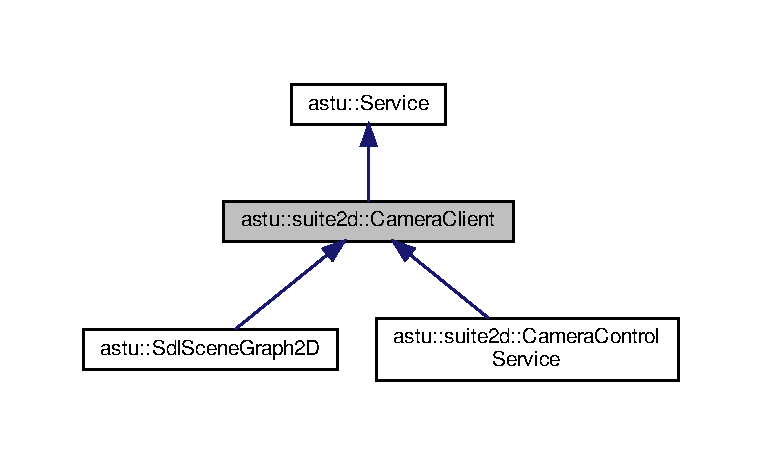
\includegraphics[width=350pt]{classastu_1_1suite2d_1_1CameraClient__inherit__graph}
\end{center}
\end{figure}


Collaboration diagram for astu\+:\+:suite2d\+:\+:Camera\+Client\+:\nopagebreak
\begin{figure}[H]
\begin{center}
\leavevmode
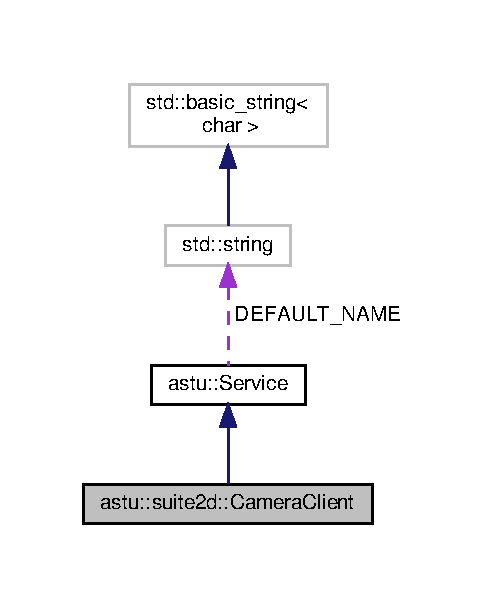
\includegraphics[width=234pt]{classastu_1_1suite2d_1_1CameraClient__coll__graph}
\end{center}
\end{figure}
\subsection*{Public Member Functions}
\begin{DoxyCompactItemize}
\item 
\hyperlink{classastu_1_1suite2d_1_1CameraClient_abed64b5a569bcdce2303bd929958eb8c}{Camera\+Client} (const std\+::string \&camera\+Name=\hyperlink{classastu_1_1suite2d_1_1CameraService_ae92f5163a54b2ab8dd738cadee8f75eb}{Camera\+Service\+::\+D\+E\+F\+A\+U\+L\+T\+\_\+\+C\+A\+M\+E\+RA}, bool create\+Camera=false)
\item 
\hyperlink{classastu_1_1suite2d_1_1Camera}{Camera} \& \hyperlink{classastu_1_1suite2d_1_1CameraClient_ac305ddbdf19d60d260a0d8af57d8a1d0}{Get\+Camera} ()
\item 
const \hyperlink{classastu_1_1suite2d_1_1Camera}{Camera} \& \hyperlink{classastu_1_1suite2d_1_1CameraClient_ae5a13bfdb3cd466404c94546bb2aeaff}{Get\+Camera} () const
\item 
void \hyperlink{classastu_1_1suite2d_1_1CameraClient_a729197722ac1f2d71f0f11708eef6204}{Use\+Camera} (const std\+::string \&cam\+Name, bool create=false)
\item 
const std\+::string \& \hyperlink{classastu_1_1suite2d_1_1CameraClient_a24450a64720a3f05ba457082171ee5f8}{Get\+Camera\+Name} () const
\end{DoxyCompactItemize}
\subsection*{Additional Inherited Members}


\subsection{Detailed Description}
A service can derive from this class if it requires access to a two-\/dimensional camera object. 

\subsection{Constructor \& Destructor Documentation}
\mbox{\Hypertarget{classastu_1_1suite2d_1_1CameraClient_abed64b5a569bcdce2303bd929958eb8c}\label{classastu_1_1suite2d_1_1CameraClient_abed64b5a569bcdce2303bd929958eb8c}} 
\index{astu\+::suite2d\+::\+Camera\+Client@{astu\+::suite2d\+::\+Camera\+Client}!Camera\+Client@{Camera\+Client}}
\index{Camera\+Client@{Camera\+Client}!astu\+::suite2d\+::\+Camera\+Client@{astu\+::suite2d\+::\+Camera\+Client}}
\subsubsection{\texorpdfstring{Camera\+Client()}{CameraClient()}}
{\footnotesize\ttfamily astu\+::suite2d\+::\+Camera\+Client\+::\+Camera\+Client (\begin{DoxyParamCaption}\item[{const std\+::string \&}]{camera\+Name = {\ttfamily \hyperlink{classastu_1_1suite2d_1_1CameraService_ae92f5163a54b2ab8dd738cadee8f75eb}{Camera\+Service\+::\+D\+E\+F\+A\+U\+L\+T\+\_\+\+C\+A\+M\+E\+RA}},  }\item[{bool}]{create\+Camera = {\ttfamily false} }\end{DoxyParamCaption})}

Constructor.


\begin{DoxyParams}{Parameters}
{\em camera\+Name} & the name of the camera to be used \\
\hline
{\em create\+Camera} & whether the camera should be created \\
\hline
\end{DoxyParams}


\subsection{Member Function Documentation}
\mbox{\Hypertarget{classastu_1_1suite2d_1_1CameraClient_ac305ddbdf19d60d260a0d8af57d8a1d0}\label{classastu_1_1suite2d_1_1CameraClient_ac305ddbdf19d60d260a0d8af57d8a1d0}} 
\index{astu\+::suite2d\+::\+Camera\+Client@{astu\+::suite2d\+::\+Camera\+Client}!Get\+Camera@{Get\+Camera}}
\index{Get\+Camera@{Get\+Camera}!astu\+::suite2d\+::\+Camera\+Client@{astu\+::suite2d\+::\+Camera\+Client}}
\subsubsection{\texorpdfstring{Get\+Camera()}{GetCamera()}\hspace{0.1cm}{\footnotesize\ttfamily [1/2]}}
{\footnotesize\ttfamily \hyperlink{classastu_1_1suite2d_1_1Camera}{Camera}\& astu\+::suite2d\+::\+Camera\+Client\+::\+Get\+Camera (\begin{DoxyParamCaption}{ }\end{DoxyParamCaption})\hspace{0.3cm}{\ttfamily [inline]}}

Returne the camera this client uses.

\begin{DoxyReturn}{Returns}
the used camera 
\end{DoxyReturn}
\mbox{\Hypertarget{classastu_1_1suite2d_1_1CameraClient_ae5a13bfdb3cd466404c94546bb2aeaff}\label{classastu_1_1suite2d_1_1CameraClient_ae5a13bfdb3cd466404c94546bb2aeaff}} 
\index{astu\+::suite2d\+::\+Camera\+Client@{astu\+::suite2d\+::\+Camera\+Client}!Get\+Camera@{Get\+Camera}}
\index{Get\+Camera@{Get\+Camera}!astu\+::suite2d\+::\+Camera\+Client@{astu\+::suite2d\+::\+Camera\+Client}}
\subsubsection{\texorpdfstring{Get\+Camera()}{GetCamera()}\hspace{0.1cm}{\footnotesize\ttfamily [2/2]}}
{\footnotesize\ttfamily const \hyperlink{classastu_1_1suite2d_1_1Camera}{Camera}\& astu\+::suite2d\+::\+Camera\+Client\+::\+Get\+Camera (\begin{DoxyParamCaption}{ }\end{DoxyParamCaption}) const\hspace{0.3cm}{\ttfamily [inline]}}

Returne the camera this client uses.

\begin{DoxyReturn}{Returns}
the used camera 
\end{DoxyReturn}
\mbox{\Hypertarget{classastu_1_1suite2d_1_1CameraClient_a24450a64720a3f05ba457082171ee5f8}\label{classastu_1_1suite2d_1_1CameraClient_a24450a64720a3f05ba457082171ee5f8}} 
\index{astu\+::suite2d\+::\+Camera\+Client@{astu\+::suite2d\+::\+Camera\+Client}!Get\+Camera\+Name@{Get\+Camera\+Name}}
\index{Get\+Camera\+Name@{Get\+Camera\+Name}!astu\+::suite2d\+::\+Camera\+Client@{astu\+::suite2d\+::\+Camera\+Client}}
\subsubsection{\texorpdfstring{Get\+Camera\+Name()}{GetCameraName()}}
{\footnotesize\ttfamily const std\+::string\& astu\+::suite2d\+::\+Camera\+Client\+::\+Get\+Camera\+Name (\begin{DoxyParamCaption}{ }\end{DoxyParamCaption}) const}

Returns the name of the camera to be used.

\begin{DoxyReturn}{Returns}
the name of the camera 
\end{DoxyReturn}
\mbox{\Hypertarget{classastu_1_1suite2d_1_1CameraClient_a729197722ac1f2d71f0f11708eef6204}\label{classastu_1_1suite2d_1_1CameraClient_a729197722ac1f2d71f0f11708eef6204}} 
\index{astu\+::suite2d\+::\+Camera\+Client@{astu\+::suite2d\+::\+Camera\+Client}!Use\+Camera@{Use\+Camera}}
\index{Use\+Camera@{Use\+Camera}!astu\+::suite2d\+::\+Camera\+Client@{astu\+::suite2d\+::\+Camera\+Client}}
\subsubsection{\texorpdfstring{Use\+Camera()}{UseCamera()}}
{\footnotesize\ttfamily void astu\+::suite2d\+::\+Camera\+Client\+::\+Use\+Camera (\begin{DoxyParamCaption}\item[{const std\+::string \&}]{cam\+Name,  }\item[{bool}]{create = {\ttfamily false} }\end{DoxyParamCaption})}

Specified which camera to use.


\begin{DoxyParams}{Parameters}
{\em cam\+Name} & the name of the camera \\
\hline
{\em create} & whether the camera should be created \\
\hline
\end{DoxyParams}

\begin{DoxyExceptions}{Exceptions}
{\em std\+::logic\+\_\+error} & in case the camera is unknown \\
\hline
\end{DoxyExceptions}


The documentation for this class was generated from the following file\+:\begin{DoxyCompactItemize}
\item 
include/\+Suite2\+D/Camera\+Service.\+h\end{DoxyCompactItemize}

\hypertarget{classastu_1_1suite2d_1_1CameraControlService}{}\section{astu\+:\+:suite2d\+:\+:Camera\+Control\+Service Class Reference}
\label{classastu_1_1suite2d_1_1CameraControlService}\index{astu\+::suite2d\+::\+Camera\+Control\+Service@{astu\+::suite2d\+::\+Camera\+Control\+Service}}


{\ttfamily \#include $<$Camera\+Control\+Service.\+h$>$}



Inheritance diagram for astu\+:\+:suite2d\+:\+:Camera\+Control\+Service\+:\nopagebreak
\begin{figure}[H]
\begin{center}
\leavevmode
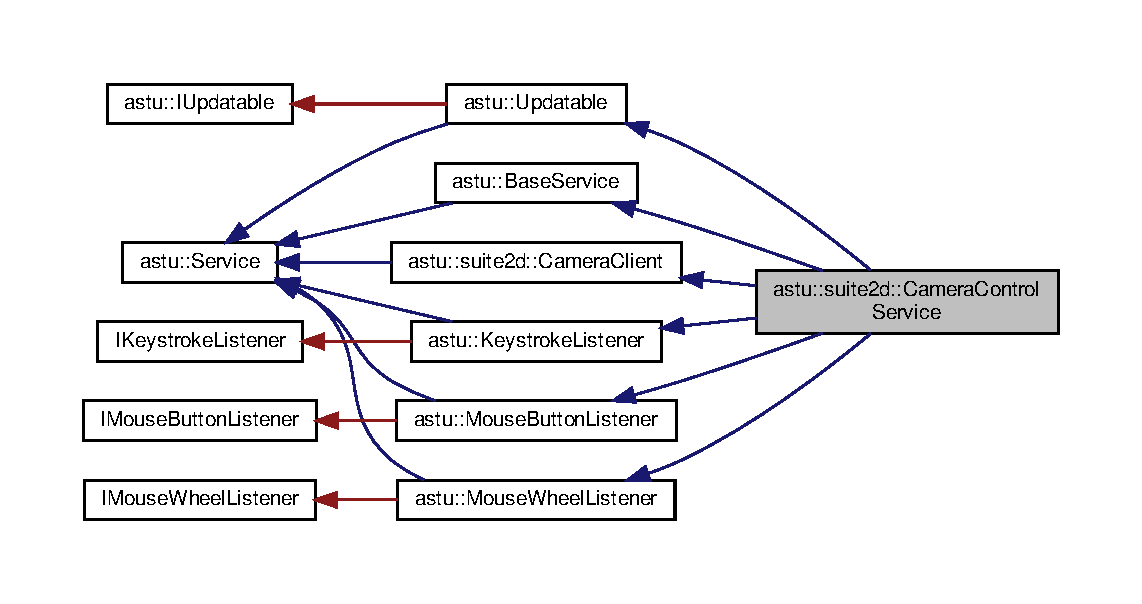
\includegraphics[width=350pt]{classastu_1_1suite2d_1_1CameraControlService__inherit__graph}
\end{center}
\end{figure}


Collaboration diagram for astu\+:\+:suite2d\+:\+:Camera\+Control\+Service\+:\nopagebreak
\begin{figure}[H]
\begin{center}
\leavevmode
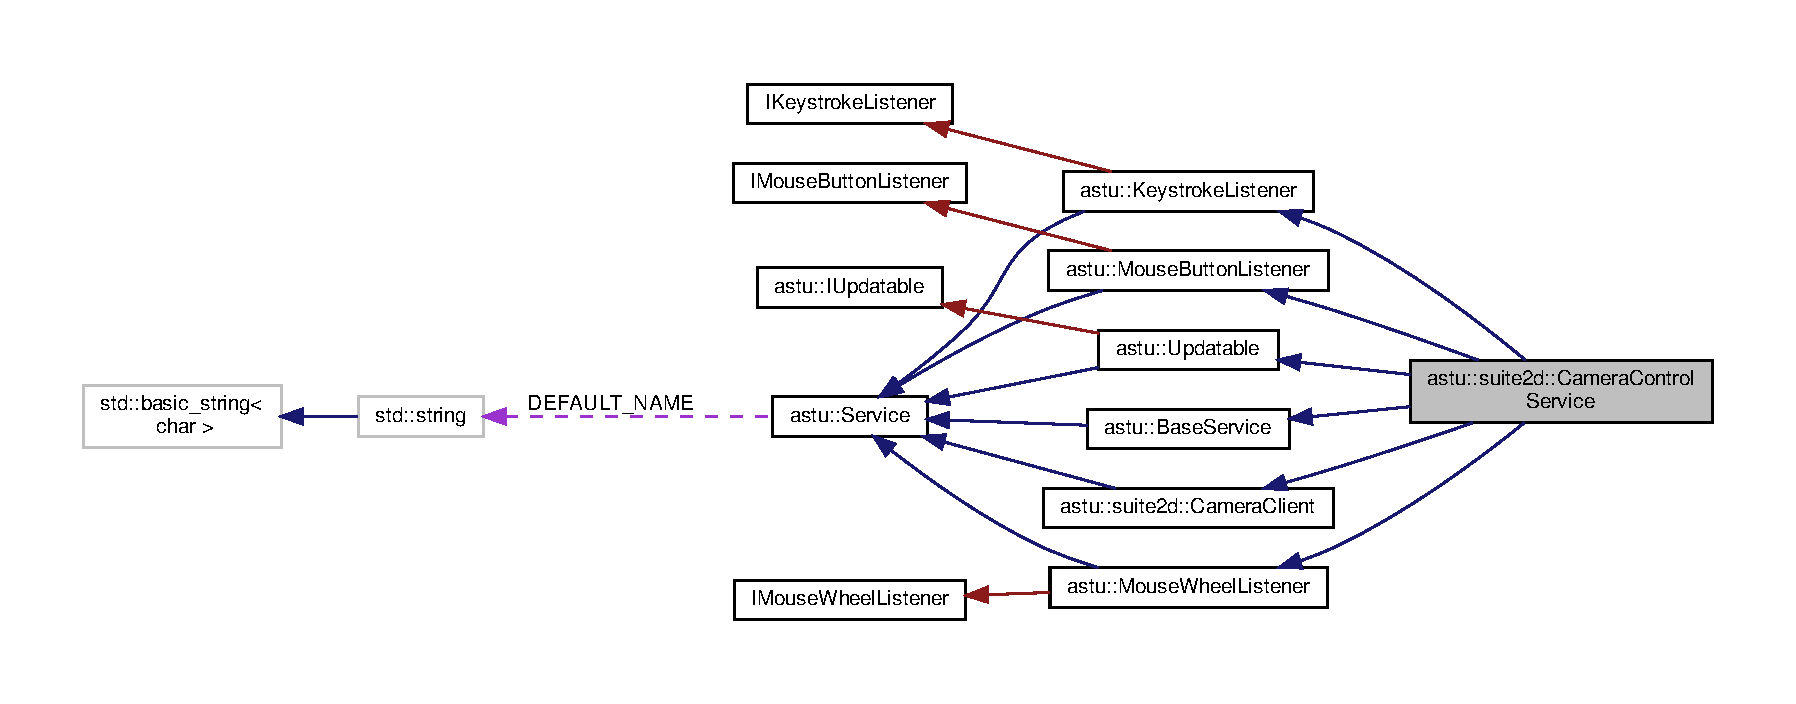
\includegraphics[width=350pt]{classastu_1_1suite2d_1_1CameraControlService__coll__graph}
\end{center}
\end{figure}
\subsection*{Public Member Functions}
\begin{DoxyCompactItemize}
\item 
\hyperlink{classastu_1_1suite2d_1_1CameraControlService_a353fcc63a3b0086216d9096cb43d5d08}{Camera\+Control\+Service} (int update\+Priority=astu\+::\+Priority\+::\+Normal)
\item 
virtual void \hyperlink{classastu_1_1suite2d_1_1CameraControlService_a7965cdf848813b62aed86ecc8c34fcc8}{On\+Startup} () override
\item 
virtual void \hyperlink{classastu_1_1suite2d_1_1CameraControlService_aaf485c9ed16494fc52ce3ebe34b1e4d9}{On\+Shutdown} () override
\item 
virtual void \hyperlink{classastu_1_1suite2d_1_1CameraControlService_ab547e4f6103448db59d1350695bed4e8}{On\+Update} () override
\item 
virtual bool \hyperlink{classastu_1_1suite2d_1_1CameraControlService_aa0a09cd56307bfab4b410ed06ffa5c74}{On\+Key\+Pressed} (int keycode) override
\item 
virtual bool \hyperlink{classastu_1_1suite2d_1_1CameraControlService_aecd396dc1d0731e9b21b9dc148e4b96b}{On\+Mouse\+Button\+Pressed} (int button, int x, int y) override
\item 
virtual bool \hyperlink{classastu_1_1suite2d_1_1CameraControlService_a4d7ad40d697e2ee2a87303032ca19333}{On\+Mouse\+Button\+Released} (int button, int x, int y) override
\item 
virtual bool \hyperlink{classastu_1_1suite2d_1_1CameraControlService_a741757d88bd6f104c71fe8f5f1a7bd69}{On\+Mouse\+Wheel} (int amount) override
\end{DoxyCompactItemize}
\subsection*{Additional Inherited Members}


\subsection{Detailed Description}
This service lets the user change the camera mode while the application is running. 

\subsection{Constructor \& Destructor Documentation}
\mbox{\Hypertarget{classastu_1_1suite2d_1_1CameraControlService_a353fcc63a3b0086216d9096cb43d5d08}\label{classastu_1_1suite2d_1_1CameraControlService_a353fcc63a3b0086216d9096cb43d5d08}} 
\index{astu\+::suite2d\+::\+Camera\+Control\+Service@{astu\+::suite2d\+::\+Camera\+Control\+Service}!Camera\+Control\+Service@{Camera\+Control\+Service}}
\index{Camera\+Control\+Service@{Camera\+Control\+Service}!astu\+::suite2d\+::\+Camera\+Control\+Service@{astu\+::suite2d\+::\+Camera\+Control\+Service}}
\subsubsection{\texorpdfstring{Camera\+Control\+Service()}{CameraControlService()}}
{\footnotesize\ttfamily astu\+::suite2d\+::\+Camera\+Control\+Service\+::\+Camera\+Control\+Service (\begin{DoxyParamCaption}\item[{int}]{update\+Priority = {\ttfamily astu\+:\+:Priority\+:\+:Normal} }\end{DoxyParamCaption})}

Constructor.


\begin{DoxyParams}{Parameters}
{\em update\+Priority} & the priority used to update this service \\
\hline
\end{DoxyParams}


\subsection{Member Function Documentation}
\mbox{\Hypertarget{classastu_1_1suite2d_1_1CameraControlService_aa0a09cd56307bfab4b410ed06ffa5c74}\label{classastu_1_1suite2d_1_1CameraControlService_aa0a09cd56307bfab4b410ed06ffa5c74}} 
\index{astu\+::suite2d\+::\+Camera\+Control\+Service@{astu\+::suite2d\+::\+Camera\+Control\+Service}!On\+Key\+Pressed@{On\+Key\+Pressed}}
\index{On\+Key\+Pressed@{On\+Key\+Pressed}!astu\+::suite2d\+::\+Camera\+Control\+Service@{astu\+::suite2d\+::\+Camera\+Control\+Service}}
\subsubsection{\texorpdfstring{On\+Key\+Pressed()}{OnKeyPressed()}}
{\footnotesize\ttfamily virtual bool astu\+::suite2d\+::\+Camera\+Control\+Service\+::\+On\+Key\+Pressed (\begin{DoxyParamCaption}\item[{int}]{keycode }\end{DoxyParamCaption})\hspace{0.3cm}{\ttfamily [override]}, {\ttfamily [virtual]}}

Called by this base class when a key has been pressed.


\begin{DoxyParams}{Parameters}
{\em keycode} & the code of the key \\
\hline
\end{DoxyParams}


Reimplemented from \hyperlink{classastu_1_1KeystrokeListener_ad4bb14ad1fd43fd200411353eeb99b5a}{astu\+::\+Keystroke\+Listener}.

\mbox{\Hypertarget{classastu_1_1suite2d_1_1CameraControlService_aecd396dc1d0731e9b21b9dc148e4b96b}\label{classastu_1_1suite2d_1_1CameraControlService_aecd396dc1d0731e9b21b9dc148e4b96b}} 
\index{astu\+::suite2d\+::\+Camera\+Control\+Service@{astu\+::suite2d\+::\+Camera\+Control\+Service}!On\+Mouse\+Button\+Pressed@{On\+Mouse\+Button\+Pressed}}
\index{On\+Mouse\+Button\+Pressed@{On\+Mouse\+Button\+Pressed}!astu\+::suite2d\+::\+Camera\+Control\+Service@{astu\+::suite2d\+::\+Camera\+Control\+Service}}
\subsubsection{\texorpdfstring{On\+Mouse\+Button\+Pressed()}{OnMouseButtonPressed()}}
{\footnotesize\ttfamily virtual bool astu\+::suite2d\+::\+Camera\+Control\+Service\+::\+On\+Mouse\+Button\+Pressed (\begin{DoxyParamCaption}\item[{int}]{button,  }\item[{int}]{x,  }\item[{int}]{y }\end{DoxyParamCaption})\hspace{0.3cm}{\ttfamily [override]}, {\ttfamily [virtual]}}

Called by this base class when a mouse button has been pressed.


\begin{DoxyParams}{Parameters}
{\em button} & the button which has been pressed \\
\hline
{\em x} & the x-\/coordinate of the mouse course in screen space \\
\hline
{\em y} & the y-\/coordinate of the mouse course in screen space \\
\hline
\end{DoxyParams}


Reimplemented from \hyperlink{classastu_1_1MouseButtonListener_abc95fea12cbecf9f8fc1f7ede14860e7}{astu\+::\+Mouse\+Button\+Listener}.

\mbox{\Hypertarget{classastu_1_1suite2d_1_1CameraControlService_a4d7ad40d697e2ee2a87303032ca19333}\label{classastu_1_1suite2d_1_1CameraControlService_a4d7ad40d697e2ee2a87303032ca19333}} 
\index{astu\+::suite2d\+::\+Camera\+Control\+Service@{astu\+::suite2d\+::\+Camera\+Control\+Service}!On\+Mouse\+Button\+Released@{On\+Mouse\+Button\+Released}}
\index{On\+Mouse\+Button\+Released@{On\+Mouse\+Button\+Released}!astu\+::suite2d\+::\+Camera\+Control\+Service@{astu\+::suite2d\+::\+Camera\+Control\+Service}}
\subsubsection{\texorpdfstring{On\+Mouse\+Button\+Released()}{OnMouseButtonReleased()}}
{\footnotesize\ttfamily virtual bool astu\+::suite2d\+::\+Camera\+Control\+Service\+::\+On\+Mouse\+Button\+Released (\begin{DoxyParamCaption}\item[{int}]{button,  }\item[{int}]{x,  }\item[{int}]{y }\end{DoxyParamCaption})\hspace{0.3cm}{\ttfamily [override]}, {\ttfamily [virtual]}}

Called by this base class when a mouse button has been released.


\begin{DoxyParams}{Parameters}
{\em button} & the button which has been released \\
\hline
{\em x} & the x-\/coordinate of the mouse course in screen space \\
\hline
{\em y} & the y-\/coordinate of the mouse course in screen space \\
\hline
\end{DoxyParams}


Reimplemented from \hyperlink{classastu_1_1MouseButtonListener_a14a97354c4f009c5f91f9877e00cef49}{astu\+::\+Mouse\+Button\+Listener}.

\mbox{\Hypertarget{classastu_1_1suite2d_1_1CameraControlService_a741757d88bd6f104c71fe8f5f1a7bd69}\label{classastu_1_1suite2d_1_1CameraControlService_a741757d88bd6f104c71fe8f5f1a7bd69}} 
\index{astu\+::suite2d\+::\+Camera\+Control\+Service@{astu\+::suite2d\+::\+Camera\+Control\+Service}!On\+Mouse\+Wheel@{On\+Mouse\+Wheel}}
\index{On\+Mouse\+Wheel@{On\+Mouse\+Wheel}!astu\+::suite2d\+::\+Camera\+Control\+Service@{astu\+::suite2d\+::\+Camera\+Control\+Service}}
\subsubsection{\texorpdfstring{On\+Mouse\+Wheel()}{OnMouseWheel()}}
{\footnotesize\ttfamily virtual bool astu\+::suite2d\+::\+Camera\+Control\+Service\+::\+On\+Mouse\+Wheel (\begin{DoxyParamCaption}\item[{int}]{amount }\end{DoxyParamCaption})\hspace{0.3cm}{\ttfamily [override]}, {\ttfamily [virtual]}}

Called by this base class when a mouse wheel signals has received.


\begin{DoxyParams}{Parameters}
{\em amount} & the amount scrolled \\
\hline
\end{DoxyParams}


Reimplemented from \hyperlink{classastu_1_1MouseWheelListener_ae159bccdfb49aadd58079fb6ce32e914}{astu\+::\+Mouse\+Wheel\+Listener}.

\mbox{\Hypertarget{classastu_1_1suite2d_1_1CameraControlService_aaf485c9ed16494fc52ce3ebe34b1e4d9}\label{classastu_1_1suite2d_1_1CameraControlService_aaf485c9ed16494fc52ce3ebe34b1e4d9}} 
\index{astu\+::suite2d\+::\+Camera\+Control\+Service@{astu\+::suite2d\+::\+Camera\+Control\+Service}!On\+Shutdown@{On\+Shutdown}}
\index{On\+Shutdown@{On\+Shutdown}!astu\+::suite2d\+::\+Camera\+Control\+Service@{astu\+::suite2d\+::\+Camera\+Control\+Service}}
\subsubsection{\texorpdfstring{On\+Shutdown()}{OnShutdown()}}
{\footnotesize\ttfamily virtual void astu\+::suite2d\+::\+Camera\+Control\+Service\+::\+On\+Shutdown (\begin{DoxyParamCaption}{ }\end{DoxyParamCaption})\hspace{0.3cm}{\ttfamily [override]}, {\ttfamily [virtual]}}

Called by the service base method on shutdown.

Derived can override this method for de-\/initialization purposes, e.\+g., releasing resources, etc. 

Reimplemented from \hyperlink{classastu_1_1Service_a1e1dff727df791c57fae782d8a613c5f}{astu\+::\+Service}.

\mbox{\Hypertarget{classastu_1_1suite2d_1_1CameraControlService_a7965cdf848813b62aed86ecc8c34fcc8}\label{classastu_1_1suite2d_1_1CameraControlService_a7965cdf848813b62aed86ecc8c34fcc8}} 
\index{astu\+::suite2d\+::\+Camera\+Control\+Service@{astu\+::suite2d\+::\+Camera\+Control\+Service}!On\+Startup@{On\+Startup}}
\index{On\+Startup@{On\+Startup}!astu\+::suite2d\+::\+Camera\+Control\+Service@{astu\+::suite2d\+::\+Camera\+Control\+Service}}
\subsubsection{\texorpdfstring{On\+Startup()}{OnStartup()}}
{\footnotesize\ttfamily virtual void astu\+::suite2d\+::\+Camera\+Control\+Service\+::\+On\+Startup (\begin{DoxyParamCaption}{ }\end{DoxyParamCaption})\hspace{0.3cm}{\ttfamily [override]}, {\ttfamily [virtual]}}

Called by the service base class on startup.

Derived can override this method for initialization purposes. 

Reimplemented from \hyperlink{classastu_1_1Service_a357dc663e000b1f086f681ec3c459bfe}{astu\+::\+Service}.

\mbox{\Hypertarget{classastu_1_1suite2d_1_1CameraControlService_ab547e4f6103448db59d1350695bed4e8}\label{classastu_1_1suite2d_1_1CameraControlService_ab547e4f6103448db59d1350695bed4e8}} 
\index{astu\+::suite2d\+::\+Camera\+Control\+Service@{astu\+::suite2d\+::\+Camera\+Control\+Service}!On\+Update@{On\+Update}}
\index{On\+Update@{On\+Update}!astu\+::suite2d\+::\+Camera\+Control\+Service@{astu\+::suite2d\+::\+Camera\+Control\+Service}}
\subsubsection{\texorpdfstring{On\+Update()}{OnUpdate()}}
{\footnotesize\ttfamily virtual void astu\+::suite2d\+::\+Camera\+Control\+Service\+::\+On\+Update (\begin{DoxyParamCaption}{ }\end{DoxyParamCaption})\hspace{0.3cm}{\ttfamily [override]}, {\ttfamily [virtual]}}

Called when an update is due. 

Reimplemented from \hyperlink{classastu_1_1Updatable_a925566c9770b95895c6c7294f9d51528}{astu\+::\+Updatable}.



The documentation for this class was generated from the following file\+:\begin{DoxyCompactItemize}
\item 
include/\+Suite2\+D/Camera\+Control\+Service.\+h\end{DoxyCompactItemize}

\hypertarget{classastu_1_1suite2d_1_1CameraService}{}\section{astu\+:\+:suite2d\+:\+:Camera\+Service Class Reference}
\label{classastu_1_1suite2d_1_1CameraService}\index{astu\+::suite2d\+::\+Camera\+Service@{astu\+::suite2d\+::\+Camera\+Service}}


{\ttfamily \#include $<$Camera\+Service.\+h$>$}



Inheritance diagram for astu\+:\+:suite2d\+:\+:Camera\+Service\+:\nopagebreak
\begin{figure}[H]
\begin{center}
\leavevmode
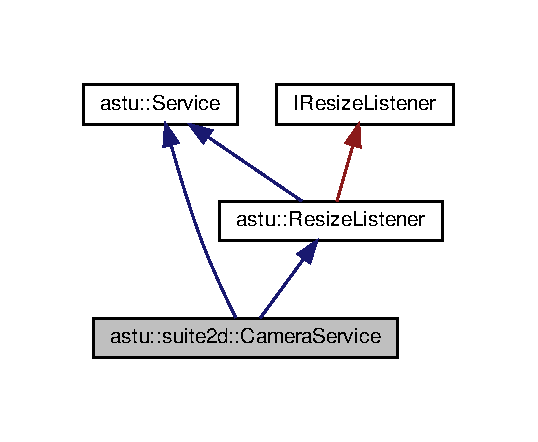
\includegraphics[width=258pt]{classastu_1_1suite2d_1_1CameraService__inherit__graph}
\end{center}
\end{figure}


Collaboration diagram for astu\+:\+:suite2d\+:\+:Camera\+Service\+:\nopagebreak
\begin{figure}[H]
\begin{center}
\leavevmode
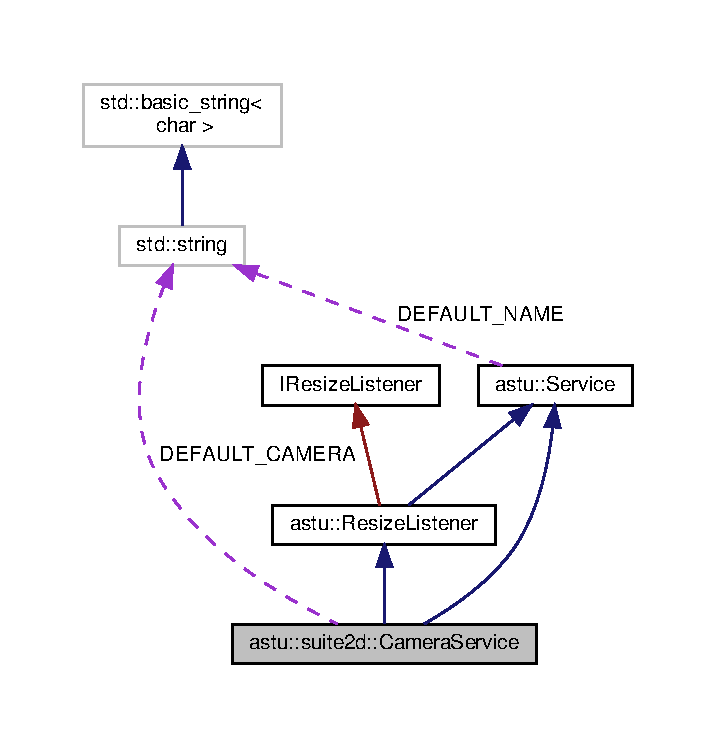
\includegraphics[width=344pt]{classastu_1_1suite2d_1_1CameraService__coll__graph}
\end{center}
\end{figure}
\subsection*{Public Member Functions}
\begin{DoxyCompactItemize}
\item 
\hyperlink{classastu_1_1suite2d_1_1CameraService_a2c77c9b8dbc01ef54797cb4c58569a50}{Camera\+Service} ()
\item 
std\+::shared\+\_\+ptr$<$ \hyperlink{classastu_1_1suite2d_1_1Camera}{Camera} $>$ \hyperlink{classastu_1_1suite2d_1_1CameraService_a6a249aa14317fe758898db2114bd9848}{Create\+Camera} (const std\+::string \&cam\+Name)
\item 
std\+::shared\+\_\+ptr$<$ \hyperlink{classastu_1_1suite2d_1_1Camera}{Camera} $>$ \hyperlink{classastu_1_1suite2d_1_1CameraService_a4ded9fceaa3da9f887f3de7810f301c7}{Get\+Camera} (const std\+::string \&cam\+Name=\hyperlink{classastu_1_1suite2d_1_1CameraService_ae92f5163a54b2ab8dd738cadee8f75eb}{D\+E\+F\+A\+U\+L\+T\+\_\+\+C\+A\+M\+E\+RA})
\item 
bool \hyperlink{classastu_1_1suite2d_1_1CameraService_a00f6b9d4898b70f7412efb21acd91271}{Has\+Camera} (const std\+::string \&cam\+Name) const
\item 
std\+::shared\+\_\+ptr$<$ \hyperlink{classastu_1_1suite2d_1_1Camera}{Camera} $>$ \hyperlink{classastu_1_1suite2d_1_1CameraService_aacd4b3d010851ebc0d3cce0453f87624}{Get\+Or\+Create\+Camera} (const std\+::string \&cam\+Name)
\item 
void \hyperlink{classastu_1_1suite2d_1_1CameraService_a7a7d3b4a1fcbfd7c1a3d2b6db1d33d82}{Destroy\+All} ()
\item 
virtual void \hyperlink{classastu_1_1suite2d_1_1CameraService_ac86690e80a0d6805abde747e501460ee}{On\+Startup} () override
\item 
virtual void \hyperlink{classastu_1_1suite2d_1_1CameraService_ae820e7576e925c559b773bb0dbd5f091}{On\+Shutdown} () override
\item 
virtual bool \hyperlink{classastu_1_1suite2d_1_1CameraService_a4229a725df31a9e416240f4b32040cdd}{On\+Resize} (int width, int height) override
\end{DoxyCompactItemize}
\subsection*{Static Public Attributes}
\begin{DoxyCompactItemize}
\item 
static const std\+::string \hyperlink{classastu_1_1suite2d_1_1CameraService_ae92f5163a54b2ab8dd738cadee8f75eb}{D\+E\+F\+A\+U\+L\+T\+\_\+\+C\+A\+M\+E\+RA}
\end{DoxyCompactItemize}
\subsection*{Additional Inherited Members}


\subsection{Detailed Description}
The camera service manages various camera objects. Cameras are created with a specific name and can be retrieved using this name. 

\subsection{Constructor \& Destructor Documentation}
\mbox{\Hypertarget{classastu_1_1suite2d_1_1CameraService_a2c77c9b8dbc01ef54797cb4c58569a50}\label{classastu_1_1suite2d_1_1CameraService_a2c77c9b8dbc01ef54797cb4c58569a50}} 
\index{astu\+::suite2d\+::\+Camera\+Service@{astu\+::suite2d\+::\+Camera\+Service}!Camera\+Service@{Camera\+Service}}
\index{Camera\+Service@{Camera\+Service}!astu\+::suite2d\+::\+Camera\+Service@{astu\+::suite2d\+::\+Camera\+Service}}
\subsubsection{\texorpdfstring{Camera\+Service()}{CameraService()}}
{\footnotesize\ttfamily astu\+::suite2d\+::\+Camera\+Service\+::\+Camera\+Service (\begin{DoxyParamCaption}{ }\end{DoxyParamCaption})}

Constructor. 

\subsection{Member Function Documentation}
\mbox{\Hypertarget{classastu_1_1suite2d_1_1CameraService_a6a249aa14317fe758898db2114bd9848}\label{classastu_1_1suite2d_1_1CameraService_a6a249aa14317fe758898db2114bd9848}} 
\index{astu\+::suite2d\+::\+Camera\+Service@{astu\+::suite2d\+::\+Camera\+Service}!Create\+Camera@{Create\+Camera}}
\index{Create\+Camera@{Create\+Camera}!astu\+::suite2d\+::\+Camera\+Service@{astu\+::suite2d\+::\+Camera\+Service}}
\subsubsection{\texorpdfstring{Create\+Camera()}{CreateCamera()}}
{\footnotesize\ttfamily std\+::shared\+\_\+ptr$<$\hyperlink{classastu_1_1suite2d_1_1Camera}{Camera}$>$ astu\+::suite2d\+::\+Camera\+Service\+::\+Create\+Camera (\begin{DoxyParamCaption}\item[{const std\+::string \&}]{cam\+Name }\end{DoxyParamCaption})}

Creates a new camera with the specified name.


\begin{DoxyParams}{Parameters}
{\em cam\+Name} & the name of the camera to create \\
\hline
\end{DoxyParams}
\begin{DoxyReturn}{Returns}
the newly created camera 
\end{DoxyReturn}

\begin{DoxyExceptions}{Exceptions}
{\em std\+::logic\+\_\+error} & in case a camera with that name already exists \\
\hline
\end{DoxyExceptions}
\mbox{\Hypertarget{classastu_1_1suite2d_1_1CameraService_a7a7d3b4a1fcbfd7c1a3d2b6db1d33d82}\label{classastu_1_1suite2d_1_1CameraService_a7a7d3b4a1fcbfd7c1a3d2b6db1d33d82}} 
\index{astu\+::suite2d\+::\+Camera\+Service@{astu\+::suite2d\+::\+Camera\+Service}!Destroy\+All@{Destroy\+All}}
\index{Destroy\+All@{Destroy\+All}!astu\+::suite2d\+::\+Camera\+Service@{astu\+::suite2d\+::\+Camera\+Service}}
\subsubsection{\texorpdfstring{Destroy\+All()}{DestroyAll()}}
{\footnotesize\ttfamily void astu\+::suite2d\+::\+Camera\+Service\+::\+Destroy\+All (\begin{DoxyParamCaption}{ }\end{DoxyParamCaption})}

Destroys all cameras. \mbox{\Hypertarget{classastu_1_1suite2d_1_1CameraService_a4ded9fceaa3da9f887f3de7810f301c7}\label{classastu_1_1suite2d_1_1CameraService_a4ded9fceaa3da9f887f3de7810f301c7}} 
\index{astu\+::suite2d\+::\+Camera\+Service@{astu\+::suite2d\+::\+Camera\+Service}!Get\+Camera@{Get\+Camera}}
\index{Get\+Camera@{Get\+Camera}!astu\+::suite2d\+::\+Camera\+Service@{astu\+::suite2d\+::\+Camera\+Service}}
\subsubsection{\texorpdfstring{Get\+Camera()}{GetCamera()}}
{\footnotesize\ttfamily std\+::shared\+\_\+ptr$<$\hyperlink{classastu_1_1suite2d_1_1Camera}{Camera}$>$ astu\+::suite2d\+::\+Camera\+Service\+::\+Get\+Camera (\begin{DoxyParamCaption}\item[{const std\+::string \&}]{cam\+Name = {\ttfamily \hyperlink{classastu_1_1suite2d_1_1CameraService_ae92f5163a54b2ab8dd738cadee8f75eb}{D\+E\+F\+A\+U\+L\+T\+\_\+\+C\+A\+M\+E\+RA}} }\end{DoxyParamCaption})}

Retrieves the camera with the specified name.


\begin{DoxyParams}{Parameters}
{\em cam\+Name} & the name of the camera \\
\hline
\end{DoxyParams}
\begin{DoxyReturn}{Returns}
the requested camera 
\end{DoxyReturn}

\begin{DoxyExceptions}{Exceptions}
{\em std\+::logic\+\_\+error} & in case the camera is unknown \\
\hline
\end{DoxyExceptions}
\mbox{\Hypertarget{classastu_1_1suite2d_1_1CameraService_aacd4b3d010851ebc0d3cce0453f87624}\label{classastu_1_1suite2d_1_1CameraService_aacd4b3d010851ebc0d3cce0453f87624}} 
\index{astu\+::suite2d\+::\+Camera\+Service@{astu\+::suite2d\+::\+Camera\+Service}!Get\+Or\+Create\+Camera@{Get\+Or\+Create\+Camera}}
\index{Get\+Or\+Create\+Camera@{Get\+Or\+Create\+Camera}!astu\+::suite2d\+::\+Camera\+Service@{astu\+::suite2d\+::\+Camera\+Service}}
\subsubsection{\texorpdfstring{Get\+Or\+Create\+Camera()}{GetOrCreateCamera()}}
{\footnotesize\ttfamily std\+::shared\+\_\+ptr$<$\hyperlink{classastu_1_1suite2d_1_1Camera}{Camera}$>$ astu\+::suite2d\+::\+Camera\+Service\+::\+Get\+Or\+Create\+Camera (\begin{DoxyParamCaption}\item[{const std\+::string \&}]{cam\+Name }\end{DoxyParamCaption})\hspace{0.3cm}{\ttfamily [inline]}}

Retrieves a camera with the specified name or creates it.


\begin{DoxyParams}{Parameters}
{\em cam\+Name} & the name of the camera \\
\hline
\end{DoxyParams}
\begin{DoxyReturn}{Returns}
the retrieved or newly created camera 
\end{DoxyReturn}
\mbox{\Hypertarget{classastu_1_1suite2d_1_1CameraService_a00f6b9d4898b70f7412efb21acd91271}\label{classastu_1_1suite2d_1_1CameraService_a00f6b9d4898b70f7412efb21acd91271}} 
\index{astu\+::suite2d\+::\+Camera\+Service@{astu\+::suite2d\+::\+Camera\+Service}!Has\+Camera@{Has\+Camera}}
\index{Has\+Camera@{Has\+Camera}!astu\+::suite2d\+::\+Camera\+Service@{astu\+::suite2d\+::\+Camera\+Service}}
\subsubsection{\texorpdfstring{Has\+Camera()}{HasCamera()}}
{\footnotesize\ttfamily bool astu\+::suite2d\+::\+Camera\+Service\+::\+Has\+Camera (\begin{DoxyParamCaption}\item[{const std\+::string \&}]{cam\+Name }\end{DoxyParamCaption}) const}

Tests whether a camera with the specified name exists.


\begin{DoxyParams}{Parameters}
{\em cam\+Name} & the name of the camera \\
\hline
\end{DoxyParams}
\begin{DoxyReturn}{Returns}
{\ttfamily true} if the camera exists 
\end{DoxyReturn}
\mbox{\Hypertarget{classastu_1_1suite2d_1_1CameraService_a4229a725df31a9e416240f4b32040cdd}\label{classastu_1_1suite2d_1_1CameraService_a4229a725df31a9e416240f4b32040cdd}} 
\index{astu\+::suite2d\+::\+Camera\+Service@{astu\+::suite2d\+::\+Camera\+Service}!On\+Resize@{On\+Resize}}
\index{On\+Resize@{On\+Resize}!astu\+::suite2d\+::\+Camera\+Service@{astu\+::suite2d\+::\+Camera\+Service}}
\subsubsection{\texorpdfstring{On\+Resize()}{OnResize()}}
{\footnotesize\ttfamily virtual bool astu\+::suite2d\+::\+Camera\+Service\+::\+On\+Resize (\begin{DoxyParamCaption}\item[{int}]{width,  }\item[{int}]{height }\end{DoxyParamCaption})\hspace{0.3cm}{\ttfamily [override]}, {\ttfamily [virtual]}}

Called by this base class when a resize signal has received.


\begin{DoxyParams}{Parameters}
{\em width} & the new window width \\
\hline
{\em height} & the new window height \\
\hline
\end{DoxyParams}


Reimplemented from \hyperlink{classastu_1_1ResizeListener_a34f14538388fdd36713cd1097dcf5fb1}{astu\+::\+Resize\+Listener}.

\mbox{\Hypertarget{classastu_1_1suite2d_1_1CameraService_ae820e7576e925c559b773bb0dbd5f091}\label{classastu_1_1suite2d_1_1CameraService_ae820e7576e925c559b773bb0dbd5f091}} 
\index{astu\+::suite2d\+::\+Camera\+Service@{astu\+::suite2d\+::\+Camera\+Service}!On\+Shutdown@{On\+Shutdown}}
\index{On\+Shutdown@{On\+Shutdown}!astu\+::suite2d\+::\+Camera\+Service@{astu\+::suite2d\+::\+Camera\+Service}}
\subsubsection{\texorpdfstring{On\+Shutdown()}{OnShutdown()}}
{\footnotesize\ttfamily virtual void astu\+::suite2d\+::\+Camera\+Service\+::\+On\+Shutdown (\begin{DoxyParamCaption}{ }\end{DoxyParamCaption})\hspace{0.3cm}{\ttfamily [override]}, {\ttfamily [virtual]}}

Called by the service base method on shutdown.

Derived can override this method for de-\/initialization purposes, e.\+g., releasing resources, etc. 

Reimplemented from \hyperlink{classastu_1_1Service_a1e1dff727df791c57fae782d8a613c5f}{astu\+::\+Service}.

\mbox{\Hypertarget{classastu_1_1suite2d_1_1CameraService_ac86690e80a0d6805abde747e501460ee}\label{classastu_1_1suite2d_1_1CameraService_ac86690e80a0d6805abde747e501460ee}} 
\index{astu\+::suite2d\+::\+Camera\+Service@{astu\+::suite2d\+::\+Camera\+Service}!On\+Startup@{On\+Startup}}
\index{On\+Startup@{On\+Startup}!astu\+::suite2d\+::\+Camera\+Service@{astu\+::suite2d\+::\+Camera\+Service}}
\subsubsection{\texorpdfstring{On\+Startup()}{OnStartup()}}
{\footnotesize\ttfamily virtual void astu\+::suite2d\+::\+Camera\+Service\+::\+On\+Startup (\begin{DoxyParamCaption}{ }\end{DoxyParamCaption})\hspace{0.3cm}{\ttfamily [override]}, {\ttfamily [virtual]}}

Called by the service base class on startup.

Derived can override this method for initialization purposes. 

Reimplemented from \hyperlink{classastu_1_1Service_a357dc663e000b1f086f681ec3c459bfe}{astu\+::\+Service}.



\subsection{Member Data Documentation}
\mbox{\Hypertarget{classastu_1_1suite2d_1_1CameraService_ae92f5163a54b2ab8dd738cadee8f75eb}\label{classastu_1_1suite2d_1_1CameraService_ae92f5163a54b2ab8dd738cadee8f75eb}} 
\index{astu\+::suite2d\+::\+Camera\+Service@{astu\+::suite2d\+::\+Camera\+Service}!D\+E\+F\+A\+U\+L\+T\+\_\+\+C\+A\+M\+E\+RA@{D\+E\+F\+A\+U\+L\+T\+\_\+\+C\+A\+M\+E\+RA}}
\index{D\+E\+F\+A\+U\+L\+T\+\_\+\+C\+A\+M\+E\+RA@{D\+E\+F\+A\+U\+L\+T\+\_\+\+C\+A\+M\+E\+RA}!astu\+::suite2d\+::\+Camera\+Service@{astu\+::suite2d\+::\+Camera\+Service}}
\subsubsection{\texorpdfstring{D\+E\+F\+A\+U\+L\+T\+\_\+\+C\+A\+M\+E\+RA}{DEFAULT\_CAMERA}}
{\footnotesize\ttfamily const std\+::string astu\+::suite2d\+::\+Camera\+Service\+::\+D\+E\+F\+A\+U\+L\+T\+\_\+\+C\+A\+M\+E\+RA\hspace{0.3cm}{\ttfamily [static]}}

The name of the default camera. 

The documentation for this class was generated from the following file\+:\begin{DoxyCompactItemize}
\item 
include/\+Suite2\+D/Camera\+Service.\+h\end{DoxyCompactItemize}

\hypertarget{classastu_1_1CAutoDestruct}{}\section{astu\+:\+:C\+Auto\+Destruct Class Reference}
\label{classastu_1_1CAutoDestruct}\index{astu\+::\+C\+Auto\+Destruct@{astu\+::\+C\+Auto\+Destruct}}


{\ttfamily \#include $<$C\+Auto\+Destruct.\+h$>$}



Inheritance diagram for astu\+:\+:C\+Auto\+Destruct\+:
\nopagebreak
\begin{figure}[H]
\begin{center}
\leavevmode
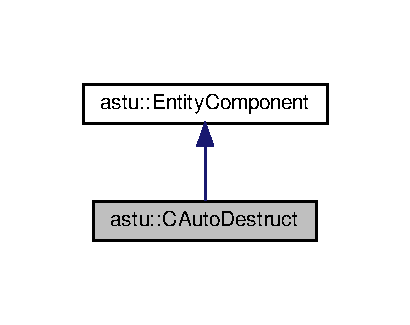
\includegraphics[width=197pt]{classastu_1_1CAutoDestruct__inherit__graph}
\end{center}
\end{figure}


Collaboration diagram for astu\+:\+:C\+Auto\+Destruct\+:
\nopagebreak
\begin{figure}[H]
\begin{center}
\leavevmode
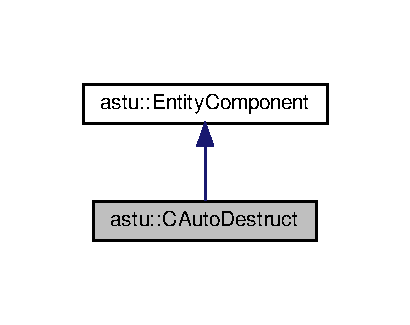
\includegraphics[width=197pt]{classastu_1_1CAutoDestruct__coll__graph}
\end{center}
\end{figure}
\subsection*{Public Member Functions}
\begin{DoxyCompactItemize}
\item 
\mbox{\Hypertarget{classastu_1_1CAutoDestruct_a0a2c5d8a934749548f6b65a91b782e9f}\label{classastu_1_1CAutoDestruct_a0a2c5d8a934749548f6b65a91b782e9f}} 
{\bfseries C\+Auto\+Destruct} (float duration)
\item 
virtual std\+::shared\+\_\+ptr$<$ \hyperlink{classastu_1_1EntityComponent}{Entity\+Component} $>$ \hyperlink{classastu_1_1CAutoDestruct_a25a9d187d42fbc3fd16311f74894b345}{Clone} () override
\end{DoxyCompactItemize}
\subsection*{Public Attributes}
\begin{DoxyCompactItemize}
\item 
\mbox{\Hypertarget{classastu_1_1CAutoDestruct_aebb5078e1e061e1c3dcbe82d1c949c58}\label{classastu_1_1CAutoDestruct_aebb5078e1e061e1c3dcbe82d1c949c58}} 
float {\bfseries duration}
\end{DoxyCompactItemize}


\subsection{Detailed Description}
This entity component describes when the entity should be removed. 

\subsection{Member Function Documentation}
\mbox{\Hypertarget{classastu_1_1CAutoDestruct_a25a9d187d42fbc3fd16311f74894b345}\label{classastu_1_1CAutoDestruct_a25a9d187d42fbc3fd16311f74894b345}} 
\index{astu\+::\+C\+Auto\+Destruct@{astu\+::\+C\+Auto\+Destruct}!Clone@{Clone}}
\index{Clone@{Clone}!astu\+::\+C\+Auto\+Destruct@{astu\+::\+C\+Auto\+Destruct}}
\subsubsection{\texorpdfstring{Clone()}{Clone()}}
{\footnotesize\ttfamily virtual std\+::shared\+\_\+ptr$<$\hyperlink{classastu_1_1EntityComponent}{Entity\+Component}$>$ astu\+::\+C\+Auto\+Destruct\+::\+Clone (\begin{DoxyParamCaption}{ }\end{DoxyParamCaption})\hspace{0.3cm}{\ttfamily [inline]}, {\ttfamily [override]}, {\ttfamily [virtual]}}

Creates a copy of this entity component.

\begin{DoxyReturn}{Returns}
a copy of this componend 
\end{DoxyReturn}


Implements \hyperlink{classastu_1_1EntityComponent_afeddb5a899d831255a9a4f07269f3b2d}{astu\+::\+Entity\+Component}.



The documentation for this class was generated from the following file\+:\begin{DoxyCompactItemize}
\item 
include/\+E\+C\+S/C\+Auto\+Destruct.\+h\end{DoxyCompactItemize}

\hypertarget{classastu_1_1suite2d_1_1CAutoRotate}{}\section{astu\+:\+:suite2d\+:\+:C\+Auto\+Rotate Class Reference}
\label{classastu_1_1suite2d_1_1CAutoRotate}\index{astu\+::suite2d\+::\+C\+Auto\+Rotate@{astu\+::suite2d\+::\+C\+Auto\+Rotate}}


{\ttfamily \#include $<$C\+Auto\+Rotate.\+h$>$}



Inheritance diagram for astu\+:\+:suite2d\+:\+:C\+Auto\+Rotate\+:\nopagebreak
\begin{figure}[H]
\begin{center}
\leavevmode
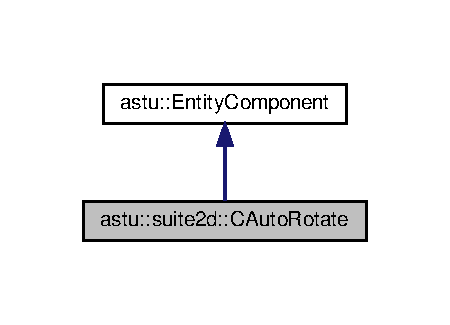
\includegraphics[width=216pt]{classastu_1_1suite2d_1_1CAutoRotate__inherit__graph}
\end{center}
\end{figure}


Collaboration diagram for astu\+:\+:suite2d\+:\+:C\+Auto\+Rotate\+:\nopagebreak
\begin{figure}[H]
\begin{center}
\leavevmode
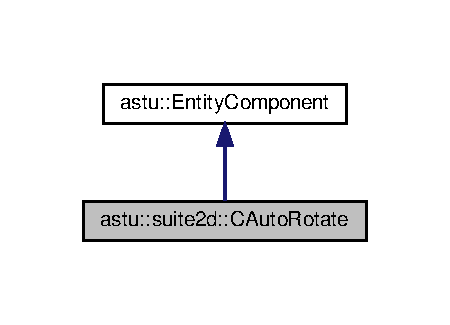
\includegraphics[width=216pt]{classastu_1_1suite2d_1_1CAutoRotate__coll__graph}
\end{center}
\end{figure}
\subsection*{Public Member Functions}
\begin{DoxyCompactItemize}
\item 
\hyperlink{classastu_1_1suite2d_1_1CAutoRotate_a53a16efe41829470f66eb471d2f196ce}{C\+Auto\+Rotate} (float \hyperlink{classastu_1_1suite2d_1_1CAutoRotate_a5757c237b7c9b14fdc43ff763e7b899b}{speed})
\item 
virtual std\+::shared\+\_\+ptr$<$ \hyperlink{classastu_1_1EntityComponent}{Entity\+Component} $>$ \hyperlink{classastu_1_1suite2d_1_1CAutoRotate_af130721018671489c7de3f652ffcc8cf}{Clone} () override
\end{DoxyCompactItemize}
\subsection*{Public Attributes}
\begin{DoxyCompactItemize}
\item 
float \hyperlink{classastu_1_1suite2d_1_1CAutoRotate_a5757c237b7c9b14fdc43ff763e7b899b}{speed}
\end{DoxyCompactItemize}


\subsection{Detailed Description}
Auto-\/\+Rotate components make entities rotate with a certain speed. 

\subsection{Constructor \& Destructor Documentation}
\mbox{\Hypertarget{classastu_1_1suite2d_1_1CAutoRotate_a53a16efe41829470f66eb471d2f196ce}\label{classastu_1_1suite2d_1_1CAutoRotate_a53a16efe41829470f66eb471d2f196ce}} 
\index{astu\+::suite2d\+::\+C\+Auto\+Rotate@{astu\+::suite2d\+::\+C\+Auto\+Rotate}!C\+Auto\+Rotate@{C\+Auto\+Rotate}}
\index{C\+Auto\+Rotate@{C\+Auto\+Rotate}!astu\+::suite2d\+::\+C\+Auto\+Rotate@{astu\+::suite2d\+::\+C\+Auto\+Rotate}}
\subsubsection{\texorpdfstring{C\+Auto\+Rotate()}{CAutoRotate()}}
{\footnotesize\ttfamily astu\+::suite2d\+::\+C\+Auto\+Rotate\+::\+C\+Auto\+Rotate (\begin{DoxyParamCaption}\item[{float}]{speed }\end{DoxyParamCaption})\hspace{0.3cm}{\ttfamily [inline]}}

Constructor.


\begin{DoxyParams}{Parameters}
{\em speed} & the angular speed in radians per second \\
\hline
\end{DoxyParams}


\subsection{Member Function Documentation}
\mbox{\Hypertarget{classastu_1_1suite2d_1_1CAutoRotate_af130721018671489c7de3f652ffcc8cf}\label{classastu_1_1suite2d_1_1CAutoRotate_af130721018671489c7de3f652ffcc8cf}} 
\index{astu\+::suite2d\+::\+C\+Auto\+Rotate@{astu\+::suite2d\+::\+C\+Auto\+Rotate}!Clone@{Clone}}
\index{Clone@{Clone}!astu\+::suite2d\+::\+C\+Auto\+Rotate@{astu\+::suite2d\+::\+C\+Auto\+Rotate}}
\subsubsection{\texorpdfstring{Clone()}{Clone()}}
{\footnotesize\ttfamily virtual std\+::shared\+\_\+ptr$<$\hyperlink{classastu_1_1EntityComponent}{Entity\+Component}$>$ astu\+::suite2d\+::\+C\+Auto\+Rotate\+::\+Clone (\begin{DoxyParamCaption}{ }\end{DoxyParamCaption})\hspace{0.3cm}{\ttfamily [inline]}, {\ttfamily [override]}, {\ttfamily [virtual]}}

Creates a copy of this entity component.

\begin{DoxyReturn}{Returns}
a copy of this componend 
\end{DoxyReturn}


Implements \hyperlink{classastu_1_1EntityComponent_afeddb5a899d831255a9a4f07269f3b2d}{astu\+::\+Entity\+Component}.



\subsection{Member Data Documentation}
\mbox{\Hypertarget{classastu_1_1suite2d_1_1CAutoRotate_a5757c237b7c9b14fdc43ff763e7b899b}\label{classastu_1_1suite2d_1_1CAutoRotate_a5757c237b7c9b14fdc43ff763e7b899b}} 
\index{astu\+::suite2d\+::\+C\+Auto\+Rotate@{astu\+::suite2d\+::\+C\+Auto\+Rotate}!speed@{speed}}
\index{speed@{speed}!astu\+::suite2d\+::\+C\+Auto\+Rotate@{astu\+::suite2d\+::\+C\+Auto\+Rotate}}
\subsubsection{\texorpdfstring{speed}{speed}}
{\footnotesize\ttfamily float astu\+::suite2d\+::\+C\+Auto\+Rotate\+::speed}

The angular speed of this auto rotate component in radians/second. 

The documentation for this class was generated from the following file\+:\begin{DoxyCompactItemize}
\item 
include/\+Suite2\+D/C\+Auto\+Rotate.\+h\end{DoxyCompactItemize}

\hypertarget{classastu_1_1suite2d_1_1CBody}{}\section{astu\+:\+:suite2d\+:\+:C\+Body Class Reference}
\label{classastu_1_1suite2d_1_1CBody}\index{astu\+::suite2d\+::\+C\+Body@{astu\+::suite2d\+::\+C\+Body}}


{\ttfamily \#include $<$C\+Body.\+h$>$}



Inheritance diagram for astu\+:\+:suite2d\+:\+:C\+Body\+:\nopagebreak
\begin{figure}[H]
\begin{center}
\leavevmode
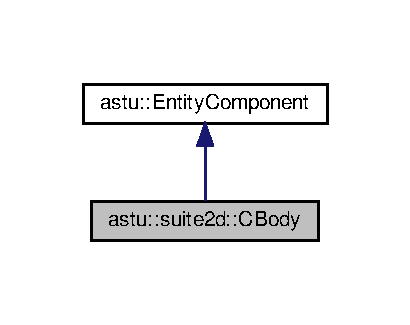
\includegraphics[width=197pt]{classastu_1_1suite2d_1_1CBody__inherit__graph}
\end{center}
\end{figure}


Collaboration diagram for astu\+:\+:suite2d\+:\+:C\+Body\+:\nopagebreak
\begin{figure}[H]
\begin{center}
\leavevmode
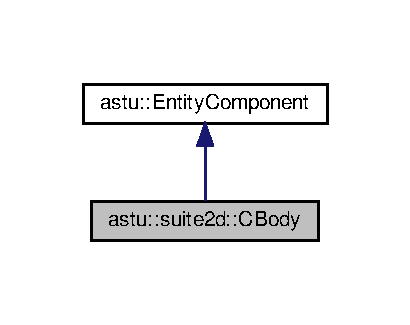
\includegraphics[width=197pt]{classastu_1_1suite2d_1_1CBody__coll__graph}
\end{center}
\end{figure}
\subsection*{Public Types}
\begin{DoxyCompactItemize}
\item 
enum \hyperlink{classastu_1_1suite2d_1_1CBody_a5731a8b9f24de5494683e4b7e8016b64}{Type} \{ \hyperlink{classastu_1_1suite2d_1_1CBody_a5731a8b9f24de5494683e4b7e8016b64af11e421e6150d5b5ca5d6acd23a5788c}{Static}, 
\hyperlink{classastu_1_1suite2d_1_1CBody_a5731a8b9f24de5494683e4b7e8016b64a56e490d706815393fb1366fc216fc335}{Kinematic}, 
\hyperlink{classastu_1_1suite2d_1_1CBody_a5731a8b9f24de5494683e4b7e8016b64a2b0c48f2b7bcf72769f693727d77f029}{Dynamic}
 \}
\end{DoxyCompactItemize}
\subsection*{Public Member Functions}
\begin{DoxyCompactItemize}
\item 
\hyperlink{classastu_1_1suite2d_1_1CBody_adbd7ed8d654abbd79242f7979d31e2d0}{C\+Body} ()
\item 
\hyperlink{classastu_1_1suite2d_1_1CBody_a5731a8b9f24de5494683e4b7e8016b64}{Type} \hyperlink{classastu_1_1suite2d_1_1CBody_a78f429bf50e5ece567478212cad5e652}{Get\+Type} () const
\item 
virtual void \hyperlink{classastu_1_1suite2d_1_1CBody_a7bc4b66e64442095a7b5ef4c689e6ccd}{Set\+Type} (\hyperlink{classastu_1_1suite2d_1_1CBody_a5731a8b9f24de5494683e4b7e8016b64}{Type} body\+Type)
\item 
virtual void \hyperlink{classastu_1_1suite2d_1_1CBody_a6c05f3452c985e94b78e198ea8b78c98}{Set\+Linear\+Velocity} (const \hyperlink{classastu_1_1Vector2}{Vector2f} \&v)
\item 
virtual \hyperlink{classastu_1_1suite2d_1_1CBody}{C\+Body} \& \hyperlink{classastu_1_1suite2d_1_1CBody_a782e16301f7268e7a511df7cdf39e168}{Set\+Linear\+Velocity} (float vx, float vy)
\item 
virtual \hyperlink{classastu_1_1Vector2}{Vector2f} \hyperlink{classastu_1_1suite2d_1_1CBody_a210a80c6f3e024b98dd367a35415cc86}{Get\+Linear\+Velocity} () const
\item 
virtual \hyperlink{classastu_1_1suite2d_1_1CBody}{C\+Body} \& \hyperlink{classastu_1_1suite2d_1_1CBody_aa99d91083ba8072acab5d1d042882d8a}{Set\+Angular\+Velocity} (float av)
\item 
virtual float \hyperlink{classastu_1_1suite2d_1_1CBody_a8b29b3752942062468e9f91f6b72430d}{Get\+Angular\+Velocity} () const
\item 
float \hyperlink{classastu_1_1suite2d_1_1CBody_ac76f056ff08398c9057563e0d67a5f00}{Get\+Linear\+Damping} () const
\item 
virtual void \hyperlink{classastu_1_1suite2d_1_1CBody_a078a4f6dbcad8717341a7ebb861a8fb2}{Set\+Linear\+Damping} (float damping)
\item 
float \hyperlink{classastu_1_1suite2d_1_1CBody_a29017bd14847bdc5f8075de0a519938e}{Get\+Angular\+Damping} () const
\item 
virtual void \hyperlink{classastu_1_1suite2d_1_1CBody_ac0edc18b2988e0ea50466dd373a61856}{Set\+Angular\+Damping} (float damping)
\item 
\hyperlink{classastu_1_1Vector2}{Vector2f} \hyperlink{classastu_1_1suite2d_1_1CBody_a1ea8700e76d0c4f46aeb0c60bc0ea2c0}{Get\+World\+Vector} (const \hyperlink{classastu_1_1Vector2}{Vector2f} \&local\+Vector)
\item 
virtual \hyperlink{classastu_1_1Vector2}{Vector2f} \hyperlink{classastu_1_1suite2d_1_1CBody_a50fb6c9131bd42e20def02619526fdff}{Get\+World\+Vector} (float lvx, float lvy)=0
\item 
\hyperlink{classastu_1_1Vector2}{Vector2f} \hyperlink{classastu_1_1suite2d_1_1CBody_a05b6ac1a2b425cf4dad2924204707029}{Get\+World\+Point} (const \hyperlink{classastu_1_1Vector2}{Vector2f} \&local\+Point)
\item 
virtual \hyperlink{classastu_1_1Vector2}{Vector2f} \hyperlink{classastu_1_1suite2d_1_1CBody_a65c7a152ab2666e355bad3116c8f910b}{Get\+World\+Point} (float lpx, float lpy)=0
\item 
\hyperlink{classastu_1_1Vector2}{Vector2f} \hyperlink{classastu_1_1suite2d_1_1CBody_a0a03263c71e5d82a26b7e20f5cf99d5d}{Get\+Local\+Vector} (const \hyperlink{classastu_1_1Vector2}{Vector2f} \&world\+Vector)
\item 
virtual \hyperlink{classastu_1_1Vector2}{Vector2f} \hyperlink{classastu_1_1suite2d_1_1CBody_a9c1d354449c29648dc07640c7853c37d}{Get\+Local\+Vector} (float wvx, float wvy)=0
\item 
\hyperlink{classastu_1_1Vector2}{Vector2f} \hyperlink{classastu_1_1suite2d_1_1CBody_a76733d539daf6c60c595586bc72db5b7}{Get\+Local\+Point} (const \hyperlink{classastu_1_1Vector2}{Vector2f} \&world\+Point)
\item 
virtual \hyperlink{classastu_1_1Vector2}{Vector2f} \hyperlink{classastu_1_1suite2d_1_1CBody_ab8945dc57ee548799613860ebac8b87c}{Get\+Local\+Point} (float wpx, float wpy)=0
\item 
virtual void \hyperlink{classastu_1_1suite2d_1_1CBody_a12f4b86353c5ed3adabbd900f2c43dba}{Apply\+Torque} (float torque)=0
\item 
virtual void \hyperlink{classastu_1_1suite2d_1_1CBody_a093468615f7e9de0b55e7af7aca2cf5e}{Apply\+Force} (const \hyperlink{classastu_1_1Vector2}{Vector2f} \&force)=0
\end{DoxyCompactItemize}


\subsection{Detailed Description}
Base class for physics based point masses in two-\/dimensional worlds. 

\subsection{Member Enumeration Documentation}
\mbox{\Hypertarget{classastu_1_1suite2d_1_1CBody_a5731a8b9f24de5494683e4b7e8016b64}\label{classastu_1_1suite2d_1_1CBody_a5731a8b9f24de5494683e4b7e8016b64}} 
\index{astu\+::suite2d\+::\+C\+Body@{astu\+::suite2d\+::\+C\+Body}!Type@{Type}}
\index{Type@{Type}!astu\+::suite2d\+::\+C\+Body@{astu\+::suite2d\+::\+C\+Body}}
\subsubsection{\texorpdfstring{Type}{Type}}
{\footnotesize\ttfamily enum \hyperlink{classastu_1_1suite2d_1_1CBody_a5731a8b9f24de5494683e4b7e8016b64}{astu\+::suite2d\+::\+C\+Body\+::\+Type}}

Enumeration describing the type of physics bodies. \begin{DoxyEnumFields}{Enumerator}
\raisebox{\heightof{T}}[0pt][0pt]{\index{Static@{Static}!astu\+::suite2d\+::\+C\+Body@{astu\+::suite2d\+::\+C\+Body}}\index{astu\+::suite2d\+::\+C\+Body@{astu\+::suite2d\+::\+C\+Body}!Static@{Static}}}\mbox{\Hypertarget{classastu_1_1suite2d_1_1CBody_a5731a8b9f24de5494683e4b7e8016b64af11e421e6150d5b5ca5d6acd23a5788c}\label{classastu_1_1suite2d_1_1CBody_a5731a8b9f24de5494683e4b7e8016b64af11e421e6150d5b5ca5d6acd23a5788c}} 
Static&Static bodies that never move. \\
\hline

\raisebox{\heightof{T}}[0pt][0pt]{\index{Kinematic@{Kinematic}!astu\+::suite2d\+::\+C\+Body@{astu\+::suite2d\+::\+C\+Body}}\index{astu\+::suite2d\+::\+C\+Body@{astu\+::suite2d\+::\+C\+Body}!Kinematic@{Kinematic}}}\mbox{\Hypertarget{classastu_1_1suite2d_1_1CBody_a5731a8b9f24de5494683e4b7e8016b64a56e490d706815393fb1366fc216fc335}\label{classastu_1_1suite2d_1_1CBody_a5731a8b9f24de5494683e4b7e8016b64a56e490d706815393fb1366fc216fc335}} 
Kinematic&Kinematic bodies can be moved by the game logic. \\
\hline

\raisebox{\heightof{T}}[0pt][0pt]{\index{Dynamic@{Dynamic}!astu\+::suite2d\+::\+C\+Body@{astu\+::suite2d\+::\+C\+Body}}\index{astu\+::suite2d\+::\+C\+Body@{astu\+::suite2d\+::\+C\+Body}!Dynamic@{Dynamic}}}\mbox{\Hypertarget{classastu_1_1suite2d_1_1CBody_a5731a8b9f24de5494683e4b7e8016b64a2b0c48f2b7bcf72769f693727d77f029}\label{classastu_1_1suite2d_1_1CBody_a5731a8b9f24de5494683e4b7e8016b64a2b0c48f2b7bcf72769f693727d77f029}} 
Dynamic&Dynamic bodies get moved by the physics system. \\
\hline

\end{DoxyEnumFields}


\subsection{Constructor \& Destructor Documentation}
\mbox{\Hypertarget{classastu_1_1suite2d_1_1CBody_adbd7ed8d654abbd79242f7979d31e2d0}\label{classastu_1_1suite2d_1_1CBody_adbd7ed8d654abbd79242f7979d31e2d0}} 
\index{astu\+::suite2d\+::\+C\+Body@{astu\+::suite2d\+::\+C\+Body}!C\+Body@{C\+Body}}
\index{C\+Body@{C\+Body}!astu\+::suite2d\+::\+C\+Body@{astu\+::suite2d\+::\+C\+Body}}
\subsubsection{\texorpdfstring{C\+Body()}{CBody()}}
{\footnotesize\ttfamily astu\+::suite2d\+::\+C\+Body\+::\+C\+Body (\begin{DoxyParamCaption}{ }\end{DoxyParamCaption})\hspace{0.3cm}{\ttfamily [inline]}}

Constructor. 

\subsection{Member Function Documentation}
\mbox{\Hypertarget{classastu_1_1suite2d_1_1CBody_a093468615f7e9de0b55e7af7aca2cf5e}\label{classastu_1_1suite2d_1_1CBody_a093468615f7e9de0b55e7af7aca2cf5e}} 
\index{astu\+::suite2d\+::\+C\+Body@{astu\+::suite2d\+::\+C\+Body}!Apply\+Force@{Apply\+Force}}
\index{Apply\+Force@{Apply\+Force}!astu\+::suite2d\+::\+C\+Body@{astu\+::suite2d\+::\+C\+Body}}
\subsubsection{\texorpdfstring{Apply\+Force()}{ApplyForce()}}
{\footnotesize\ttfamily virtual void astu\+::suite2d\+::\+C\+Body\+::\+Apply\+Force (\begin{DoxyParamCaption}\item[{const \hyperlink{classastu_1_1Vector2}{Vector2f} \&}]{force }\end{DoxyParamCaption})\hspace{0.3cm}{\ttfamily [pure virtual]}}

Applies a force at the center of mass.


\begin{DoxyParams}{Parameters}
{\em force} & the force vector in world space, usually in Newtons \\
\hline
\end{DoxyParams}
\mbox{\Hypertarget{classastu_1_1suite2d_1_1CBody_a12f4b86353c5ed3adabbd900f2c43dba}\label{classastu_1_1suite2d_1_1CBody_a12f4b86353c5ed3adabbd900f2c43dba}} 
\index{astu\+::suite2d\+::\+C\+Body@{astu\+::suite2d\+::\+C\+Body}!Apply\+Torque@{Apply\+Torque}}
\index{Apply\+Torque@{Apply\+Torque}!astu\+::suite2d\+::\+C\+Body@{astu\+::suite2d\+::\+C\+Body}}
\subsubsection{\texorpdfstring{Apply\+Torque()}{ApplyTorque()}}
{\footnotesize\ttfamily virtual void astu\+::suite2d\+::\+C\+Body\+::\+Apply\+Torque (\begin{DoxyParamCaption}\item[{float}]{torque }\end{DoxyParamCaption})\hspace{0.3cm}{\ttfamily [pure virtual]}}

Applies a torque to this body.


\begin{DoxyParams}{Parameters}
{\em torque} & the torque to apply, usually in N-\/m. \\
\hline
\end{DoxyParams}
\mbox{\Hypertarget{classastu_1_1suite2d_1_1CBody_a29017bd14847bdc5f8075de0a519938e}\label{classastu_1_1suite2d_1_1CBody_a29017bd14847bdc5f8075de0a519938e}} 
\index{astu\+::suite2d\+::\+C\+Body@{astu\+::suite2d\+::\+C\+Body}!Get\+Angular\+Damping@{Get\+Angular\+Damping}}
\index{Get\+Angular\+Damping@{Get\+Angular\+Damping}!astu\+::suite2d\+::\+C\+Body@{astu\+::suite2d\+::\+C\+Body}}
\subsubsection{\texorpdfstring{Get\+Angular\+Damping()}{GetAngularDamping()}}
{\footnotesize\ttfamily float astu\+::suite2d\+::\+C\+Body\+::\+Get\+Angular\+Damping (\begin{DoxyParamCaption}{ }\end{DoxyParamCaption}) const\hspace{0.3cm}{\ttfamily [inline]}}

Returns the angular damping of this body.

\begin{DoxyReturn}{Returns}
the angular damping 
\end{DoxyReturn}
\mbox{\Hypertarget{classastu_1_1suite2d_1_1CBody_a8b29b3752942062468e9f91f6b72430d}\label{classastu_1_1suite2d_1_1CBody_a8b29b3752942062468e9f91f6b72430d}} 
\index{astu\+::suite2d\+::\+C\+Body@{astu\+::suite2d\+::\+C\+Body}!Get\+Angular\+Velocity@{Get\+Angular\+Velocity}}
\index{Get\+Angular\+Velocity@{Get\+Angular\+Velocity}!astu\+::suite2d\+::\+C\+Body@{astu\+::suite2d\+::\+C\+Body}}
\subsubsection{\texorpdfstring{Get\+Angular\+Velocity()}{GetAngularVelocity()}}
{\footnotesize\ttfamily virtual float astu\+::suite2d\+::\+C\+Body\+::\+Get\+Angular\+Velocity (\begin{DoxyParamCaption}{ }\end{DoxyParamCaption}) const\hspace{0.3cm}{\ttfamily [inline]}, {\ttfamily [virtual]}}

Returns the angular velocity of this body.

\begin{DoxyReturn}{Returns}
the angular velocity 
\end{DoxyReturn}
\mbox{\Hypertarget{classastu_1_1suite2d_1_1CBody_ac76f056ff08398c9057563e0d67a5f00}\label{classastu_1_1suite2d_1_1CBody_ac76f056ff08398c9057563e0d67a5f00}} 
\index{astu\+::suite2d\+::\+C\+Body@{astu\+::suite2d\+::\+C\+Body}!Get\+Linear\+Damping@{Get\+Linear\+Damping}}
\index{Get\+Linear\+Damping@{Get\+Linear\+Damping}!astu\+::suite2d\+::\+C\+Body@{astu\+::suite2d\+::\+C\+Body}}
\subsubsection{\texorpdfstring{Get\+Linear\+Damping()}{GetLinearDamping()}}
{\footnotesize\ttfamily float astu\+::suite2d\+::\+C\+Body\+::\+Get\+Linear\+Damping (\begin{DoxyParamCaption}{ }\end{DoxyParamCaption}) const\hspace{0.3cm}{\ttfamily [inline]}}

Returns the linear damping of this body.

\begin{DoxyReturn}{Returns}
the linear damping 
\end{DoxyReturn}
\mbox{\Hypertarget{classastu_1_1suite2d_1_1CBody_a210a80c6f3e024b98dd367a35415cc86}\label{classastu_1_1suite2d_1_1CBody_a210a80c6f3e024b98dd367a35415cc86}} 
\index{astu\+::suite2d\+::\+C\+Body@{astu\+::suite2d\+::\+C\+Body}!Get\+Linear\+Velocity@{Get\+Linear\+Velocity}}
\index{Get\+Linear\+Velocity@{Get\+Linear\+Velocity}!astu\+::suite2d\+::\+C\+Body@{astu\+::suite2d\+::\+C\+Body}}
\subsubsection{\texorpdfstring{Get\+Linear\+Velocity()}{GetLinearVelocity()}}
{\footnotesize\ttfamily virtual \hyperlink{classastu_1_1Vector2}{Vector2f} astu\+::suite2d\+::\+C\+Body\+::\+Get\+Linear\+Velocity (\begin{DoxyParamCaption}{ }\end{DoxyParamCaption}) const\hspace{0.3cm}{\ttfamily [inline]}, {\ttfamily [virtual]}}

Returns the linear velocity at the center of mass.

\begin{DoxyReturn}{Returns}
the linear velocity 
\end{DoxyReturn}
\mbox{\Hypertarget{classastu_1_1suite2d_1_1CBody_a76733d539daf6c60c595586bc72db5b7}\label{classastu_1_1suite2d_1_1CBody_a76733d539daf6c60c595586bc72db5b7}} 
\index{astu\+::suite2d\+::\+C\+Body@{astu\+::suite2d\+::\+C\+Body}!Get\+Local\+Point@{Get\+Local\+Point}}
\index{Get\+Local\+Point@{Get\+Local\+Point}!astu\+::suite2d\+::\+C\+Body@{astu\+::suite2d\+::\+C\+Body}}
\subsubsection{\texorpdfstring{Get\+Local\+Point()}{GetLocalPoint()}\hspace{0.1cm}{\footnotesize\ttfamily [1/2]}}
{\footnotesize\ttfamily \hyperlink{classastu_1_1Vector2}{Vector2f} astu\+::suite2d\+::\+C\+Body\+::\+Get\+Local\+Point (\begin{DoxyParamCaption}\item[{const \hyperlink{classastu_1_1Vector2}{Vector2f} \&}]{world\+Point }\end{DoxyParamCaption})\hspace{0.3cm}{\ttfamily [inline]}}

Converts a point from world space to local space.


\begin{DoxyParams}{Parameters}
{\em world\+Point} & the point in world space \\
\hline
\end{DoxyParams}
\begin{DoxyReturn}{Returns}
the tranformed point in local space 
\end{DoxyReturn}
\mbox{\Hypertarget{classastu_1_1suite2d_1_1CBody_ab8945dc57ee548799613860ebac8b87c}\label{classastu_1_1suite2d_1_1CBody_ab8945dc57ee548799613860ebac8b87c}} 
\index{astu\+::suite2d\+::\+C\+Body@{astu\+::suite2d\+::\+C\+Body}!Get\+Local\+Point@{Get\+Local\+Point}}
\index{Get\+Local\+Point@{Get\+Local\+Point}!astu\+::suite2d\+::\+C\+Body@{astu\+::suite2d\+::\+C\+Body}}
\subsubsection{\texorpdfstring{Get\+Local\+Point()}{GetLocalPoint()}\hspace{0.1cm}{\footnotesize\ttfamily [2/2]}}
{\footnotesize\ttfamily virtual \hyperlink{classastu_1_1Vector2}{Vector2f} astu\+::suite2d\+::\+C\+Body\+::\+Get\+Local\+Point (\begin{DoxyParamCaption}\item[{float}]{wpx,  }\item[{float}]{wpy }\end{DoxyParamCaption})\hspace{0.3cm}{\ttfamily [pure virtual]}}

Converts a point from world space to local space.


\begin{DoxyParams}{Parameters}
{\em wpx} & the x-\/componnent of the point in world space \\
\hline
{\em wpy} & the y-\/componnent of the point in world space \\
\hline
\end{DoxyParams}
\begin{DoxyReturn}{Returns}
the tranformed point in local space 
\end{DoxyReturn}
\mbox{\Hypertarget{classastu_1_1suite2d_1_1CBody_a0a03263c71e5d82a26b7e20f5cf99d5d}\label{classastu_1_1suite2d_1_1CBody_a0a03263c71e5d82a26b7e20f5cf99d5d}} 
\index{astu\+::suite2d\+::\+C\+Body@{astu\+::suite2d\+::\+C\+Body}!Get\+Local\+Vector@{Get\+Local\+Vector}}
\index{Get\+Local\+Vector@{Get\+Local\+Vector}!astu\+::suite2d\+::\+C\+Body@{astu\+::suite2d\+::\+C\+Body}}
\subsubsection{\texorpdfstring{Get\+Local\+Vector()}{GetLocalVector()}\hspace{0.1cm}{\footnotesize\ttfamily [1/2]}}
{\footnotesize\ttfamily \hyperlink{classastu_1_1Vector2}{Vector2f} astu\+::suite2d\+::\+C\+Body\+::\+Get\+Local\+Vector (\begin{DoxyParamCaption}\item[{const \hyperlink{classastu_1_1Vector2}{Vector2f} \&}]{world\+Vector }\end{DoxyParamCaption})\hspace{0.3cm}{\ttfamily [inline]}}

Converts a vector from world space to local space.


\begin{DoxyParams}{Parameters}
{\em world\+Vector} & the vector in world space \\
\hline
\end{DoxyParams}
\begin{DoxyReturn}{Returns}
the tranformed vector in local space 
\end{DoxyReturn}
\mbox{\Hypertarget{classastu_1_1suite2d_1_1CBody_a9c1d354449c29648dc07640c7853c37d}\label{classastu_1_1suite2d_1_1CBody_a9c1d354449c29648dc07640c7853c37d}} 
\index{astu\+::suite2d\+::\+C\+Body@{astu\+::suite2d\+::\+C\+Body}!Get\+Local\+Vector@{Get\+Local\+Vector}}
\index{Get\+Local\+Vector@{Get\+Local\+Vector}!astu\+::suite2d\+::\+C\+Body@{astu\+::suite2d\+::\+C\+Body}}
\subsubsection{\texorpdfstring{Get\+Local\+Vector()}{GetLocalVector()}\hspace{0.1cm}{\footnotesize\ttfamily [2/2]}}
{\footnotesize\ttfamily virtual \hyperlink{classastu_1_1Vector2}{Vector2f} astu\+::suite2d\+::\+C\+Body\+::\+Get\+Local\+Vector (\begin{DoxyParamCaption}\item[{float}]{wvx,  }\item[{float}]{wvy }\end{DoxyParamCaption})\hspace{0.3cm}{\ttfamily [pure virtual]}}

Converts a vector from world space to local space.


\begin{DoxyParams}{Parameters}
{\em wvx} & the x-\/componnent of the vector in world space \\
\hline
{\em wvy} & the y-\/componnent of the vector in world space \\
\hline
\end{DoxyParams}
\begin{DoxyReturn}{Returns}
the tranformed vector in local space 
\end{DoxyReturn}
\mbox{\Hypertarget{classastu_1_1suite2d_1_1CBody_a78f429bf50e5ece567478212cad5e652}\label{classastu_1_1suite2d_1_1CBody_a78f429bf50e5ece567478212cad5e652}} 
\index{astu\+::suite2d\+::\+C\+Body@{astu\+::suite2d\+::\+C\+Body}!Get\+Type@{Get\+Type}}
\index{Get\+Type@{Get\+Type}!astu\+::suite2d\+::\+C\+Body@{astu\+::suite2d\+::\+C\+Body}}
\subsubsection{\texorpdfstring{Get\+Type()}{GetType()}}
{\footnotesize\ttfamily \hyperlink{classastu_1_1suite2d_1_1CBody_a5731a8b9f24de5494683e4b7e8016b64}{Type} astu\+::suite2d\+::\+C\+Body\+::\+Get\+Type (\begin{DoxyParamCaption}{ }\end{DoxyParamCaption}) const\hspace{0.3cm}{\ttfamily [inline]}}

Returns the type of this body.

\begin{DoxyReturn}{Returns}
the type of this body 
\end{DoxyReturn}
\mbox{\Hypertarget{classastu_1_1suite2d_1_1CBody_a05b6ac1a2b425cf4dad2924204707029}\label{classastu_1_1suite2d_1_1CBody_a05b6ac1a2b425cf4dad2924204707029}} 
\index{astu\+::suite2d\+::\+C\+Body@{astu\+::suite2d\+::\+C\+Body}!Get\+World\+Point@{Get\+World\+Point}}
\index{Get\+World\+Point@{Get\+World\+Point}!astu\+::suite2d\+::\+C\+Body@{astu\+::suite2d\+::\+C\+Body}}
\subsubsection{\texorpdfstring{Get\+World\+Point()}{GetWorldPoint()}\hspace{0.1cm}{\footnotesize\ttfamily [1/2]}}
{\footnotesize\ttfamily \hyperlink{classastu_1_1Vector2}{Vector2f} astu\+::suite2d\+::\+C\+Body\+::\+Get\+World\+Point (\begin{DoxyParamCaption}\item[{const \hyperlink{classastu_1_1Vector2}{Vector2f} \&}]{local\+Point }\end{DoxyParamCaption})\hspace{0.3cm}{\ttfamily [inline]}}

Converts a point from local space to world space.


\begin{DoxyParams}{Parameters}
{\em local\+Point} & the point in local space \\
\hline
\end{DoxyParams}
\begin{DoxyReturn}{Returns}
the tranformed point in world space 
\end{DoxyReturn}
\mbox{\Hypertarget{classastu_1_1suite2d_1_1CBody_a65c7a152ab2666e355bad3116c8f910b}\label{classastu_1_1suite2d_1_1CBody_a65c7a152ab2666e355bad3116c8f910b}} 
\index{astu\+::suite2d\+::\+C\+Body@{astu\+::suite2d\+::\+C\+Body}!Get\+World\+Point@{Get\+World\+Point}}
\index{Get\+World\+Point@{Get\+World\+Point}!astu\+::suite2d\+::\+C\+Body@{astu\+::suite2d\+::\+C\+Body}}
\subsubsection{\texorpdfstring{Get\+World\+Point()}{GetWorldPoint()}\hspace{0.1cm}{\footnotesize\ttfamily [2/2]}}
{\footnotesize\ttfamily virtual \hyperlink{classastu_1_1Vector2}{Vector2f} astu\+::suite2d\+::\+C\+Body\+::\+Get\+World\+Point (\begin{DoxyParamCaption}\item[{float}]{lpx,  }\item[{float}]{lpy }\end{DoxyParamCaption})\hspace{0.3cm}{\ttfamily [pure virtual]}}

Converts a point from local space to world space.


\begin{DoxyParams}{Parameters}
{\em lpx} & the x-\/componnent of the point in local space \\
\hline
{\em lpy} & the y-\/componnent of the point in local space \\
\hline
\end{DoxyParams}
\begin{DoxyReturn}{Returns}
the tranformed point in world space 
\end{DoxyReturn}
\mbox{\Hypertarget{classastu_1_1suite2d_1_1CBody_a1ea8700e76d0c4f46aeb0c60bc0ea2c0}\label{classastu_1_1suite2d_1_1CBody_a1ea8700e76d0c4f46aeb0c60bc0ea2c0}} 
\index{astu\+::suite2d\+::\+C\+Body@{astu\+::suite2d\+::\+C\+Body}!Get\+World\+Vector@{Get\+World\+Vector}}
\index{Get\+World\+Vector@{Get\+World\+Vector}!astu\+::suite2d\+::\+C\+Body@{astu\+::suite2d\+::\+C\+Body}}
\subsubsection{\texorpdfstring{Get\+World\+Vector()}{GetWorldVector()}\hspace{0.1cm}{\footnotesize\ttfamily [1/2]}}
{\footnotesize\ttfamily \hyperlink{classastu_1_1Vector2}{Vector2f} astu\+::suite2d\+::\+C\+Body\+::\+Get\+World\+Vector (\begin{DoxyParamCaption}\item[{const \hyperlink{classastu_1_1Vector2}{Vector2f} \&}]{local\+Vector }\end{DoxyParamCaption})\hspace{0.3cm}{\ttfamily [inline]}}

Converts a vector from local space to world space.


\begin{DoxyParams}{Parameters}
{\em local\+Vector} & the vector in local space \\
\hline
\end{DoxyParams}
\begin{DoxyReturn}{Returns}
the tranformed vector in world space 
\end{DoxyReturn}
\mbox{\Hypertarget{classastu_1_1suite2d_1_1CBody_a50fb6c9131bd42e20def02619526fdff}\label{classastu_1_1suite2d_1_1CBody_a50fb6c9131bd42e20def02619526fdff}} 
\index{astu\+::suite2d\+::\+C\+Body@{astu\+::suite2d\+::\+C\+Body}!Get\+World\+Vector@{Get\+World\+Vector}}
\index{Get\+World\+Vector@{Get\+World\+Vector}!astu\+::suite2d\+::\+C\+Body@{astu\+::suite2d\+::\+C\+Body}}
\subsubsection{\texorpdfstring{Get\+World\+Vector()}{GetWorldVector()}\hspace{0.1cm}{\footnotesize\ttfamily [2/2]}}
{\footnotesize\ttfamily virtual \hyperlink{classastu_1_1Vector2}{Vector2f} astu\+::suite2d\+::\+C\+Body\+::\+Get\+World\+Vector (\begin{DoxyParamCaption}\item[{float}]{lvx,  }\item[{float}]{lvy }\end{DoxyParamCaption})\hspace{0.3cm}{\ttfamily [pure virtual]}}

Converts a vector from local space to world space.


\begin{DoxyParams}{Parameters}
{\em lvx} & the x-\/componnent of the vector in local space \\
\hline
{\em lvy} & the y-\/componnent of the vector in local space \\
\hline
\end{DoxyParams}
\begin{DoxyReturn}{Returns}
the tranformed vector in world space 
\end{DoxyReturn}
\mbox{\Hypertarget{classastu_1_1suite2d_1_1CBody_ac0edc18b2988e0ea50466dd373a61856}\label{classastu_1_1suite2d_1_1CBody_ac0edc18b2988e0ea50466dd373a61856}} 
\index{astu\+::suite2d\+::\+C\+Body@{astu\+::suite2d\+::\+C\+Body}!Set\+Angular\+Damping@{Set\+Angular\+Damping}}
\index{Set\+Angular\+Damping@{Set\+Angular\+Damping}!astu\+::suite2d\+::\+C\+Body@{astu\+::suite2d\+::\+C\+Body}}
\subsubsection{\texorpdfstring{Set\+Angular\+Damping()}{SetAngularDamping()}}
{\footnotesize\ttfamily virtual void astu\+::suite2d\+::\+C\+Body\+::\+Set\+Angular\+Damping (\begin{DoxyParamCaption}\item[{float}]{damping }\end{DoxyParamCaption})\hspace{0.3cm}{\ttfamily [inline]}, {\ttfamily [virtual]}}

Sets the angular damping of this body.


\begin{DoxyParams}{Parameters}
{\em damping} & the damping for rotational movement \\
\hline
\end{DoxyParams}
\mbox{\Hypertarget{classastu_1_1suite2d_1_1CBody_aa99d91083ba8072acab5d1d042882d8a}\label{classastu_1_1suite2d_1_1CBody_aa99d91083ba8072acab5d1d042882d8a}} 
\index{astu\+::suite2d\+::\+C\+Body@{astu\+::suite2d\+::\+C\+Body}!Set\+Angular\+Velocity@{Set\+Angular\+Velocity}}
\index{Set\+Angular\+Velocity@{Set\+Angular\+Velocity}!astu\+::suite2d\+::\+C\+Body@{astu\+::suite2d\+::\+C\+Body}}
\subsubsection{\texorpdfstring{Set\+Angular\+Velocity()}{SetAngularVelocity()}}
{\footnotesize\ttfamily virtual \hyperlink{classastu_1_1suite2d_1_1CBody}{C\+Body}\& astu\+::suite2d\+::\+C\+Body\+::\+Set\+Angular\+Velocity (\begin{DoxyParamCaption}\item[{float}]{av }\end{DoxyParamCaption})\hspace{0.3cm}{\ttfamily [inline]}, {\ttfamily [virtual]}}

Sets the angular velocity.


\begin{DoxyParams}{Parameters}
{\em av} & the angular velocity in radians per second \\
\hline
\end{DoxyParams}
\mbox{\Hypertarget{classastu_1_1suite2d_1_1CBody_a078a4f6dbcad8717341a7ebb861a8fb2}\label{classastu_1_1suite2d_1_1CBody_a078a4f6dbcad8717341a7ebb861a8fb2}} 
\index{astu\+::suite2d\+::\+C\+Body@{astu\+::suite2d\+::\+C\+Body}!Set\+Linear\+Damping@{Set\+Linear\+Damping}}
\index{Set\+Linear\+Damping@{Set\+Linear\+Damping}!astu\+::suite2d\+::\+C\+Body@{astu\+::suite2d\+::\+C\+Body}}
\subsubsection{\texorpdfstring{Set\+Linear\+Damping()}{SetLinearDamping()}}
{\footnotesize\ttfamily virtual void astu\+::suite2d\+::\+C\+Body\+::\+Set\+Linear\+Damping (\begin{DoxyParamCaption}\item[{float}]{damping }\end{DoxyParamCaption})\hspace{0.3cm}{\ttfamily [inline]}, {\ttfamily [virtual]}}

Sets the linear damping of this body.


\begin{DoxyParams}{Parameters}
{\em damping} & the damping for linear movement \\
\hline
\end{DoxyParams}
\mbox{\Hypertarget{classastu_1_1suite2d_1_1CBody_a6c05f3452c985e94b78e198ea8b78c98}\label{classastu_1_1suite2d_1_1CBody_a6c05f3452c985e94b78e198ea8b78c98}} 
\index{astu\+::suite2d\+::\+C\+Body@{astu\+::suite2d\+::\+C\+Body}!Set\+Linear\+Velocity@{Set\+Linear\+Velocity}}
\index{Set\+Linear\+Velocity@{Set\+Linear\+Velocity}!astu\+::suite2d\+::\+C\+Body@{astu\+::suite2d\+::\+C\+Body}}
\subsubsection{\texorpdfstring{Set\+Linear\+Velocity()}{SetLinearVelocity()}\hspace{0.1cm}{\footnotesize\ttfamily [1/2]}}
{\footnotesize\ttfamily virtual void astu\+::suite2d\+::\+C\+Body\+::\+Set\+Linear\+Velocity (\begin{DoxyParamCaption}\item[{const \hyperlink{classastu_1_1Vector2}{Vector2f} \&}]{v }\end{DoxyParamCaption})\hspace{0.3cm}{\ttfamily [inline]}, {\ttfamily [virtual]}}

Sets the linear velocity of this body.


\begin{DoxyParams}{Parameters}
{\em v} & the linear velocity \\
\hline
\end{DoxyParams}
\mbox{\Hypertarget{classastu_1_1suite2d_1_1CBody_a782e16301f7268e7a511df7cdf39e168}\label{classastu_1_1suite2d_1_1CBody_a782e16301f7268e7a511df7cdf39e168}} 
\index{astu\+::suite2d\+::\+C\+Body@{astu\+::suite2d\+::\+C\+Body}!Set\+Linear\+Velocity@{Set\+Linear\+Velocity}}
\index{Set\+Linear\+Velocity@{Set\+Linear\+Velocity}!astu\+::suite2d\+::\+C\+Body@{astu\+::suite2d\+::\+C\+Body}}
\subsubsection{\texorpdfstring{Set\+Linear\+Velocity()}{SetLinearVelocity()}\hspace{0.1cm}{\footnotesize\ttfamily [2/2]}}
{\footnotesize\ttfamily virtual \hyperlink{classastu_1_1suite2d_1_1CBody}{C\+Body}\& astu\+::suite2d\+::\+C\+Body\+::\+Set\+Linear\+Velocity (\begin{DoxyParamCaption}\item[{float}]{vx,  }\item[{float}]{vy }\end{DoxyParamCaption})\hspace{0.3cm}{\ttfamily [inline]}, {\ttfamily [virtual]}}

Sets the linear velocity of this body.


\begin{DoxyParams}{Parameters}
{\em vx} & the x-\/component of the linear velocity \\
\hline
{\em vy} & the y-\/component of the linear velocity \\
\hline
\end{DoxyParams}
\begin{DoxyReturn}{Returns}
reference to this body for method chaining 
\end{DoxyReturn}
\mbox{\Hypertarget{classastu_1_1suite2d_1_1CBody_a7bc4b66e64442095a7b5ef4c689e6ccd}\label{classastu_1_1suite2d_1_1CBody_a7bc4b66e64442095a7b5ef4c689e6ccd}} 
\index{astu\+::suite2d\+::\+C\+Body@{astu\+::suite2d\+::\+C\+Body}!Set\+Type@{Set\+Type}}
\index{Set\+Type@{Set\+Type}!astu\+::suite2d\+::\+C\+Body@{astu\+::suite2d\+::\+C\+Body}}
\subsubsection{\texorpdfstring{Set\+Type()}{SetType()}}
{\footnotesize\ttfamily virtual void astu\+::suite2d\+::\+C\+Body\+::\+Set\+Type (\begin{DoxyParamCaption}\item[{\hyperlink{classastu_1_1suite2d_1_1CBody_a5731a8b9f24de5494683e4b7e8016b64}{Type}}]{body\+Type }\end{DoxyParamCaption})\hspace{0.3cm}{\ttfamily [inline]}, {\ttfamily [virtual]}}

Sets the type of this body.


\begin{DoxyParams}{Parameters}
{\em body\+Type} & the type of this body \\
\hline
\end{DoxyParams}


The documentation for this class was generated from the following file\+:\begin{DoxyCompactItemize}
\item 
include/\+Suite2\+D/C\+Body.\+h\end{DoxyCompactItemize}

\hypertarget{classastu_1_1suite2d_1_1CBodyBuilder}{}\section{astu\+:\+:suite2d\+:\+:C\+Body\+Builder Class Reference}
\label{classastu_1_1suite2d_1_1CBodyBuilder}\index{astu\+::suite2d\+::\+C\+Body\+Builder@{astu\+::suite2d\+::\+C\+Body\+Builder}}


{\ttfamily \#include $<$C\+Body.\+h$>$}

\subsection*{Public Member Functions}
\begin{DoxyCompactItemize}
\item 
\hyperlink{classastu_1_1suite2d_1_1CBodyBuilder_a0ca8f798e66caf8f32fec25698c2a4ef}{C\+Body\+Builder} (std\+::shared\+\_\+ptr$<$ \hyperlink{classastu_1_1suite2d_1_1CBodyFactory}{C\+Body\+Factory} $>$ body\+Factory=nullptr)
\item 
\hyperlink{classastu_1_1suite2d_1_1CBodyBuilder}{C\+Body\+Builder} \& \hyperlink{classastu_1_1suite2d_1_1CBodyBuilder_a42f2d0af41647c1617cb948d72d2fe0f}{Type} (\hyperlink{classastu_1_1suite2d_1_1CBody_a5731a8b9f24de5494683e4b7e8016b64}{C\+Body\+::\+Type} body\+Type)
\item 
\hyperlink{classastu_1_1suite2d_1_1CBodyBuilder}{C\+Body\+Builder} \& \hyperlink{classastu_1_1suite2d_1_1CBodyBuilder_a15294ce7b267061e70013553cc3c171d}{Linear\+Velocity} (float vx, float vy)
\item 
\hyperlink{classastu_1_1suite2d_1_1CBodyBuilder}{C\+Body\+Builder} \& \hyperlink{classastu_1_1suite2d_1_1CBodyBuilder_a3b30b6a22dbbace93d0867cb04131b5c}{Linear\+Velocity} (const \hyperlink{classastu_1_1Vector2}{Vector2f} \&v)
\item 
\hyperlink{classastu_1_1suite2d_1_1CBodyBuilder}{C\+Body\+Builder} \& \hyperlink{classastu_1_1suite2d_1_1CBodyBuilder_a7a8919a8033bc348a4aba8b215db8351}{Angular\+Velocity} (float av)
\item 
\hyperlink{classastu_1_1suite2d_1_1CBodyBuilder}{C\+Body\+Builder} \& \hyperlink{classastu_1_1suite2d_1_1CBodyBuilder_a8228f975cbec219125323d06fc6d0f16}{Angular\+Damping} (float damping)
\item 
\hyperlink{classastu_1_1suite2d_1_1CBodyBuilder}{C\+Body\+Builder} \& \hyperlink{classastu_1_1suite2d_1_1CBodyBuilder_af8bac26e1270985e9da41aa7f6eff9a7}{Linear\+Damping} (float damping)
\item 
\hyperlink{classastu_1_1suite2d_1_1CBodyBuilder}{C\+Body\+Builder} \& \hyperlink{classastu_1_1suite2d_1_1CBodyBuilder_aa1eba70e75a9b7ac0c915e9b2f2cdf8d}{Reset} ()
\item 
std\+::shared\+\_\+ptr$<$ \hyperlink{classastu_1_1suite2d_1_1CBody}{C\+Body} $>$ \hyperlink{classastu_1_1suite2d_1_1CBodyBuilder_a2a08001660aaa09c683a6b66d7f1a47d}{Build} ()
\end{DoxyCompactItemize}


\subsection{Detailed Description}
Builder for \hyperlink{classastu_1_1suite2d_1_1CBody}{C\+Body} components. 

\subsection{Constructor \& Destructor Documentation}
\mbox{\Hypertarget{classastu_1_1suite2d_1_1CBodyBuilder_a0ca8f798e66caf8f32fec25698c2a4ef}\label{classastu_1_1suite2d_1_1CBodyBuilder_a0ca8f798e66caf8f32fec25698c2a4ef}} 
\index{astu\+::suite2d\+::\+C\+Body\+Builder@{astu\+::suite2d\+::\+C\+Body\+Builder}!C\+Body\+Builder@{C\+Body\+Builder}}
\index{C\+Body\+Builder@{C\+Body\+Builder}!astu\+::suite2d\+::\+C\+Body\+Builder@{astu\+::suite2d\+::\+C\+Body\+Builder}}
\subsubsection{\texorpdfstring{C\+Body\+Builder()}{CBodyBuilder()}}
{\footnotesize\ttfamily astu\+::suite2d\+::\+C\+Body\+Builder\+::\+C\+Body\+Builder (\begin{DoxyParamCaption}\item[{std\+::shared\+\_\+ptr$<$ \hyperlink{classastu_1_1suite2d_1_1CBodyFactory}{C\+Body\+Factory} $>$}]{body\+Factory = {\ttfamily nullptr} }\end{DoxyParamCaption})}

Constructor.

If the specified body factory is null a service which implements the body factory interface will be used.


\begin{DoxyParams}{Parameters}
{\em body\+Factory} & the factory for \hyperlink{classastu_1_1suite2d_1_1CBody}{C\+Body} components to be used \\
\hline
\end{DoxyParams}


\subsection{Member Function Documentation}
\mbox{\Hypertarget{classastu_1_1suite2d_1_1CBodyBuilder_a8228f975cbec219125323d06fc6d0f16}\label{classastu_1_1suite2d_1_1CBodyBuilder_a8228f975cbec219125323d06fc6d0f16}} 
\index{astu\+::suite2d\+::\+C\+Body\+Builder@{astu\+::suite2d\+::\+C\+Body\+Builder}!Angular\+Damping@{Angular\+Damping}}
\index{Angular\+Damping@{Angular\+Damping}!astu\+::suite2d\+::\+C\+Body\+Builder@{astu\+::suite2d\+::\+C\+Body\+Builder}}
\subsubsection{\texorpdfstring{Angular\+Damping()}{AngularDamping()}}
{\footnotesize\ttfamily \hyperlink{classastu_1_1suite2d_1_1CBodyBuilder}{C\+Body\+Builder}\& astu\+::suite2d\+::\+C\+Body\+Builder\+::\+Angular\+Damping (\begin{DoxyParamCaption}\item[{float}]{damping }\end{DoxyParamCaption})\hspace{0.3cm}{\ttfamily [inline]}}

Sets the angular damping of the body to create


\begin{DoxyParams}{Parameters}
{\em damping} & the damping for rotational movement \\
\hline
\end{DoxyParams}
\begin{DoxyReturn}{Returns}
reference to this builder for method chaining 
\end{DoxyReturn}

\begin{DoxyExceptions}{Exceptions}
{\em std\+::domain\+\_\+error} & in case the damping is less than zero \\
\hline
\end{DoxyExceptions}
\mbox{\Hypertarget{classastu_1_1suite2d_1_1CBodyBuilder_a7a8919a8033bc348a4aba8b215db8351}\label{classastu_1_1suite2d_1_1CBodyBuilder_a7a8919a8033bc348a4aba8b215db8351}} 
\index{astu\+::suite2d\+::\+C\+Body\+Builder@{astu\+::suite2d\+::\+C\+Body\+Builder}!Angular\+Velocity@{Angular\+Velocity}}
\index{Angular\+Velocity@{Angular\+Velocity}!astu\+::suite2d\+::\+C\+Body\+Builder@{astu\+::suite2d\+::\+C\+Body\+Builder}}
\subsubsection{\texorpdfstring{Angular\+Velocity()}{AngularVelocity()}}
{\footnotesize\ttfamily \hyperlink{classastu_1_1suite2d_1_1CBodyBuilder}{C\+Body\+Builder}\& astu\+::suite2d\+::\+C\+Body\+Builder\+::\+Angular\+Velocity (\begin{DoxyParamCaption}\item[{float}]{av }\end{DoxyParamCaption})\hspace{0.3cm}{\ttfamily [inline]}}

Sets the angular velocity of the body to create body.


\begin{DoxyParams}{Parameters}
{\em av} & the angular velocity in radians per second \\
\hline
\end{DoxyParams}
\begin{DoxyReturn}{Returns}
reference to this builder for method chaining 
\end{DoxyReturn}
\mbox{\Hypertarget{classastu_1_1suite2d_1_1CBodyBuilder_a2a08001660aaa09c683a6b66d7f1a47d}\label{classastu_1_1suite2d_1_1CBodyBuilder_a2a08001660aaa09c683a6b66d7f1a47d}} 
\index{astu\+::suite2d\+::\+C\+Body\+Builder@{astu\+::suite2d\+::\+C\+Body\+Builder}!Build@{Build}}
\index{Build@{Build}!astu\+::suite2d\+::\+C\+Body\+Builder@{astu\+::suite2d\+::\+C\+Body\+Builder}}
\subsubsection{\texorpdfstring{Build()}{Build()}}
{\footnotesize\ttfamily std\+::shared\+\_\+ptr$<$\hyperlink{classastu_1_1suite2d_1_1CBody}{C\+Body}$>$ astu\+::suite2d\+::\+C\+Body\+Builder\+::\+Build (\begin{DoxyParamCaption}{ }\end{DoxyParamCaption})}

Creates a new \hyperlink{classastu_1_1suite2d_1_1CBody}{C\+Body} instance according to the current configuration.

\begin{DoxyReturn}{Returns}
the new \hyperlink{classastu_1_1suite2d_1_1CBody}{C\+Body} instance 
\end{DoxyReturn}
\mbox{\Hypertarget{classastu_1_1suite2d_1_1CBodyBuilder_af8bac26e1270985e9da41aa7f6eff9a7}\label{classastu_1_1suite2d_1_1CBodyBuilder_af8bac26e1270985e9da41aa7f6eff9a7}} 
\index{astu\+::suite2d\+::\+C\+Body\+Builder@{astu\+::suite2d\+::\+C\+Body\+Builder}!Linear\+Damping@{Linear\+Damping}}
\index{Linear\+Damping@{Linear\+Damping}!astu\+::suite2d\+::\+C\+Body\+Builder@{astu\+::suite2d\+::\+C\+Body\+Builder}}
\subsubsection{\texorpdfstring{Linear\+Damping()}{LinearDamping()}}
{\footnotesize\ttfamily \hyperlink{classastu_1_1suite2d_1_1CBodyBuilder}{C\+Body\+Builder}\& astu\+::suite2d\+::\+C\+Body\+Builder\+::\+Linear\+Damping (\begin{DoxyParamCaption}\item[{float}]{damping }\end{DoxyParamCaption})\hspace{0.3cm}{\ttfamily [inline]}}

Sets the linear damping of the body to create


\begin{DoxyParams}{Parameters}
{\em damping} & the damping for linear movement \\
\hline
\end{DoxyParams}
\begin{DoxyReturn}{Returns}
reference to this builder for method chaining 
\end{DoxyReturn}

\begin{DoxyExceptions}{Exceptions}
{\em std\+::domain\+\_\+error} & in case the damping is less than zero \\
\hline
\end{DoxyExceptions}
\mbox{\Hypertarget{classastu_1_1suite2d_1_1CBodyBuilder_a15294ce7b267061e70013553cc3c171d}\label{classastu_1_1suite2d_1_1CBodyBuilder_a15294ce7b267061e70013553cc3c171d}} 
\index{astu\+::suite2d\+::\+C\+Body\+Builder@{astu\+::suite2d\+::\+C\+Body\+Builder}!Linear\+Velocity@{Linear\+Velocity}}
\index{Linear\+Velocity@{Linear\+Velocity}!astu\+::suite2d\+::\+C\+Body\+Builder@{astu\+::suite2d\+::\+C\+Body\+Builder}}
\subsubsection{\texorpdfstring{Linear\+Velocity()}{LinearVelocity()}\hspace{0.1cm}{\footnotesize\ttfamily [1/2]}}
{\footnotesize\ttfamily \hyperlink{classastu_1_1suite2d_1_1CBodyBuilder}{C\+Body\+Builder}\& astu\+::suite2d\+::\+C\+Body\+Builder\+::\+Linear\+Velocity (\begin{DoxyParamCaption}\item[{float}]{vx,  }\item[{float}]{vy }\end{DoxyParamCaption})\hspace{0.3cm}{\ttfamily [inline]}}

Sets the linear velocity of the body to create body.


\begin{DoxyParams}{Parameters}
{\em vx} & the x-\/component of the linear velocity \\
\hline
{\em vy} & the y-\/component of the linear velocity \\
\hline
\end{DoxyParams}
\begin{DoxyReturn}{Returns}
reference to this builder for method chaining 
\end{DoxyReturn}
\mbox{\Hypertarget{classastu_1_1suite2d_1_1CBodyBuilder_a3b30b6a22dbbace93d0867cb04131b5c}\label{classastu_1_1suite2d_1_1CBodyBuilder_a3b30b6a22dbbace93d0867cb04131b5c}} 
\index{astu\+::suite2d\+::\+C\+Body\+Builder@{astu\+::suite2d\+::\+C\+Body\+Builder}!Linear\+Velocity@{Linear\+Velocity}}
\index{Linear\+Velocity@{Linear\+Velocity}!astu\+::suite2d\+::\+C\+Body\+Builder@{astu\+::suite2d\+::\+C\+Body\+Builder}}
\subsubsection{\texorpdfstring{Linear\+Velocity()}{LinearVelocity()}\hspace{0.1cm}{\footnotesize\ttfamily [2/2]}}
{\footnotesize\ttfamily \hyperlink{classastu_1_1suite2d_1_1CBodyBuilder}{C\+Body\+Builder}\& astu\+::suite2d\+::\+C\+Body\+Builder\+::\+Linear\+Velocity (\begin{DoxyParamCaption}\item[{const \hyperlink{classastu_1_1Vector2}{Vector2f} \&}]{v }\end{DoxyParamCaption})\hspace{0.3cm}{\ttfamily [inline]}}

Sets the linear velocity of the body to create body.


\begin{DoxyParams}{Parameters}
{\em v} & the velocity vector \\
\hline
\end{DoxyParams}
\begin{DoxyReturn}{Returns}
reference to this builder for method chaining 
\end{DoxyReturn}
\mbox{\Hypertarget{classastu_1_1suite2d_1_1CBodyBuilder_aa1eba70e75a9b7ac0c915e9b2f2cdf8d}\label{classastu_1_1suite2d_1_1CBodyBuilder_aa1eba70e75a9b7ac0c915e9b2f2cdf8d}} 
\index{astu\+::suite2d\+::\+C\+Body\+Builder@{astu\+::suite2d\+::\+C\+Body\+Builder}!Reset@{Reset}}
\index{Reset@{Reset}!astu\+::suite2d\+::\+C\+Body\+Builder@{astu\+::suite2d\+::\+C\+Body\+Builder}}
\subsubsection{\texorpdfstring{Reset()}{Reset()}}
{\footnotesize\ttfamily \hyperlink{classastu_1_1suite2d_1_1CBodyBuilder}{C\+Body\+Builder}\& astu\+::suite2d\+::\+C\+Body\+Builder\+::\+Reset (\begin{DoxyParamCaption}{ }\end{DoxyParamCaption})\hspace{0.3cm}{\ttfamily [inline]}}

Resets this build to its initial configuration.

\begin{DoxyReturn}{Returns}
reference to this builder for method chaining 
\end{DoxyReturn}
\mbox{\Hypertarget{classastu_1_1suite2d_1_1CBodyBuilder_a42f2d0af41647c1617cb948d72d2fe0f}\label{classastu_1_1suite2d_1_1CBodyBuilder_a42f2d0af41647c1617cb948d72d2fe0f}} 
\index{astu\+::suite2d\+::\+C\+Body\+Builder@{astu\+::suite2d\+::\+C\+Body\+Builder}!Type@{Type}}
\index{Type@{Type}!astu\+::suite2d\+::\+C\+Body\+Builder@{astu\+::suite2d\+::\+C\+Body\+Builder}}
\subsubsection{\texorpdfstring{Type()}{Type()}}
{\footnotesize\ttfamily \hyperlink{classastu_1_1suite2d_1_1CBodyBuilder}{C\+Body\+Builder}\& astu\+::suite2d\+::\+C\+Body\+Builder\+::\+Type (\begin{DoxyParamCaption}\item[{\hyperlink{classastu_1_1suite2d_1_1CBody_a5731a8b9f24de5494683e4b7e8016b64}{C\+Body\+::\+Type}}]{body\+Type }\end{DoxyParamCaption})\hspace{0.3cm}{\ttfamily [inline]}}

Sets the type of the body to create.


\begin{DoxyParams}{Parameters}
{\em body\+Type} & the type of the body \\
\hline
\end{DoxyParams}
\begin{DoxyReturn}{Returns}
reference to this builder for method chaining 
\end{DoxyReturn}


The documentation for this class was generated from the following file\+:\begin{DoxyCompactItemize}
\item 
include/\+Suite2\+D/C\+Body.\+h\end{DoxyCompactItemize}

\hypertarget{classastu_1_1suite2d_1_1CBodyCollider}{}\section{astu\+:\+:suite2d\+:\+:C\+Body\+Collider Class Reference}
\label{classastu_1_1suite2d_1_1CBodyCollider}\index{astu\+::suite2d\+::\+C\+Body\+Collider@{astu\+::suite2d\+::\+C\+Body\+Collider}}


{\ttfamily \#include $<$C\+Colliders.\+h$>$}



Inheritance diagram for astu\+:\+:suite2d\+:\+:C\+Body\+Collider\+:\nopagebreak
\begin{figure}[H]
\begin{center}
\leavevmode
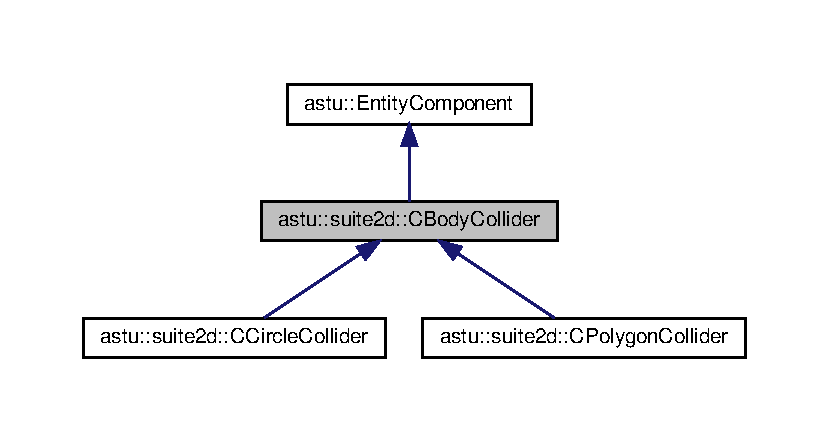
\includegraphics[width=350pt]{classastu_1_1suite2d_1_1CBodyCollider__inherit__graph}
\end{center}
\end{figure}


Collaboration diagram for astu\+:\+:suite2d\+:\+:C\+Body\+Collider\+:\nopagebreak
\begin{figure}[H]
\begin{center}
\leavevmode
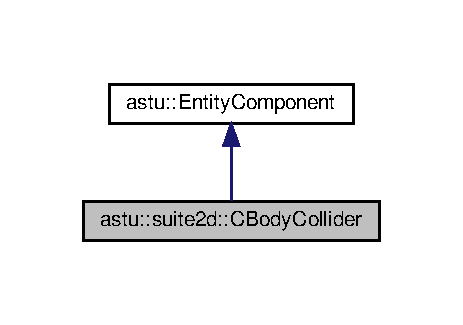
\includegraphics[width=222pt]{classastu_1_1suite2d_1_1CBodyCollider__coll__graph}
\end{center}
\end{figure}
\subsection*{Public Member Functions}
\begin{DoxyCompactItemize}
\item 
\hyperlink{classastu_1_1suite2d_1_1CBodyCollider_a53b70ad4182f2e4b6520cd4078cf55ad}{C\+Body\+Collider} ()
\item 
float \hyperlink{classastu_1_1suite2d_1_1CBodyCollider_a3323f62162d237b44858fc1ee53fa5b1}{Get\+Restitution} () const
\item 
virtual void \hyperlink{classastu_1_1suite2d_1_1CBodyCollider_a28a503811fbdcc29fe1fa6204f82bd8a}{Set\+Restitution} (float r)
\item 
float \hyperlink{classastu_1_1suite2d_1_1CBodyCollider_aa707f66fb6b9fd9ce21aedaed43837ff}{Get\+Friction} () const
\item 
virtual void \hyperlink{classastu_1_1suite2d_1_1CBodyCollider_ab457509068d608af68158417e32a023d}{Set\+Friction} (float f)
\item 
float \hyperlink{classastu_1_1suite2d_1_1CBodyCollider_a79f739655a74fd53e30f645668bd7d85}{Get\+Density} () const
\item 
virtual void \hyperlink{classastu_1_1suite2d_1_1CBodyCollider_abad2e774affa1d966ad1b1b86c76ce51}{Set\+Density} (float d)
\item 
uint16\+\_\+t \hyperlink{classastu_1_1suite2d_1_1CBodyCollider_a46d61eb00e4b1dd78790bed52fca7ac5}{Get\+Category\+Bits} () const
\item 
virtual void \hyperlink{classastu_1_1suite2d_1_1CBodyCollider_af6e02b7f4a1bd613303e0d04518e790b}{Set\+Category\+Bits} (uint16\+\_\+t bits)
\item 
uint16\+\_\+t \hyperlink{classastu_1_1suite2d_1_1CBodyCollider_a4122233f1f658f090600520ecf05ff92}{Get\+Mask\+Bits} () const
\item 
virtual void \hyperlink{classastu_1_1suite2d_1_1CBodyCollider_aa7411ba5c94adecc996d655bd38c7fb8}{Set\+Mask\+Bits} (uint16\+\_\+t bits)
\item 
const \hyperlink{classastu_1_1Vector2}{Vector2f} \& \hyperlink{classastu_1_1suite2d_1_1CBodyCollider_ad874702f1fd7b40e477916deb8f39289}{Get\+Offset} () const
\item 
virtual void \hyperlink{classastu_1_1suite2d_1_1CBodyCollider_aa0fe045b29e4207852be567b5e004c91}{Set\+Offset} (const \hyperlink{classastu_1_1Vector2}{Vector2f} \&o)
\end{DoxyCompactItemize}


\subsection{Detailed Description}
Base class for physics collider in two-\/dimensional worlds. 

\subsection{Constructor \& Destructor Documentation}
\mbox{\Hypertarget{classastu_1_1suite2d_1_1CBodyCollider_a53b70ad4182f2e4b6520cd4078cf55ad}\label{classastu_1_1suite2d_1_1CBodyCollider_a53b70ad4182f2e4b6520cd4078cf55ad}} 
\index{astu\+::suite2d\+::\+C\+Body\+Collider@{astu\+::suite2d\+::\+C\+Body\+Collider}!C\+Body\+Collider@{C\+Body\+Collider}}
\index{C\+Body\+Collider@{C\+Body\+Collider}!astu\+::suite2d\+::\+C\+Body\+Collider@{astu\+::suite2d\+::\+C\+Body\+Collider}}
\subsubsection{\texorpdfstring{C\+Body\+Collider()}{CBodyCollider()}}
{\footnotesize\ttfamily astu\+::suite2d\+::\+C\+Body\+Collider\+::\+C\+Body\+Collider (\begin{DoxyParamCaption}{ }\end{DoxyParamCaption})\hspace{0.3cm}{\ttfamily [inline]}}

Constructor. 

\subsection{Member Function Documentation}
\mbox{\Hypertarget{classastu_1_1suite2d_1_1CBodyCollider_a46d61eb00e4b1dd78790bed52fca7ac5}\label{classastu_1_1suite2d_1_1CBodyCollider_a46d61eb00e4b1dd78790bed52fca7ac5}} 
\index{astu\+::suite2d\+::\+C\+Body\+Collider@{astu\+::suite2d\+::\+C\+Body\+Collider}!Get\+Category\+Bits@{Get\+Category\+Bits}}
\index{Get\+Category\+Bits@{Get\+Category\+Bits}!astu\+::suite2d\+::\+C\+Body\+Collider@{astu\+::suite2d\+::\+C\+Body\+Collider}}
\subsubsection{\texorpdfstring{Get\+Category\+Bits()}{GetCategoryBits()}}
{\footnotesize\ttfamily uint16\+\_\+t astu\+::suite2d\+::\+C\+Body\+Collider\+::\+Get\+Category\+Bits (\begin{DoxyParamCaption}{ }\end{DoxyParamCaption}) const\hspace{0.3cm}{\ttfamily [inline]}}

Returns the category bits used for collision filtering.

\begin{DoxyReturn}{Returns}
the category bits 
\end{DoxyReturn}
\mbox{\Hypertarget{classastu_1_1suite2d_1_1CBodyCollider_a79f739655a74fd53e30f645668bd7d85}\label{classastu_1_1suite2d_1_1CBodyCollider_a79f739655a74fd53e30f645668bd7d85}} 
\index{astu\+::suite2d\+::\+C\+Body\+Collider@{astu\+::suite2d\+::\+C\+Body\+Collider}!Get\+Density@{Get\+Density}}
\index{Get\+Density@{Get\+Density}!astu\+::suite2d\+::\+C\+Body\+Collider@{astu\+::suite2d\+::\+C\+Body\+Collider}}
\subsubsection{\texorpdfstring{Get\+Density()}{GetDensity()}}
{\footnotesize\ttfamily float astu\+::suite2d\+::\+C\+Body\+Collider\+::\+Get\+Density (\begin{DoxyParamCaption}{ }\end{DoxyParamCaption}) const\hspace{0.3cm}{\ttfamily [inline]}}

Returns the density of this collider.

\begin{DoxyReturn}{Returns}
the density, usually in kg/m$^\wedge$2 
\end{DoxyReturn}
\mbox{\Hypertarget{classastu_1_1suite2d_1_1CBodyCollider_aa707f66fb6b9fd9ce21aedaed43837ff}\label{classastu_1_1suite2d_1_1CBodyCollider_aa707f66fb6b9fd9ce21aedaed43837ff}} 
\index{astu\+::suite2d\+::\+C\+Body\+Collider@{astu\+::suite2d\+::\+C\+Body\+Collider}!Get\+Friction@{Get\+Friction}}
\index{Get\+Friction@{Get\+Friction}!astu\+::suite2d\+::\+C\+Body\+Collider@{astu\+::suite2d\+::\+C\+Body\+Collider}}
\subsubsection{\texorpdfstring{Get\+Friction()}{GetFriction()}}
{\footnotesize\ttfamily float astu\+::suite2d\+::\+C\+Body\+Collider\+::\+Get\+Friction (\begin{DoxyParamCaption}{ }\end{DoxyParamCaption}) const\hspace{0.3cm}{\ttfamily [inline]}}

Returns the friction coefficient.

\begin{DoxyReturn}{Returns}
the friction coefficient 
\end{DoxyReturn}
\mbox{\Hypertarget{classastu_1_1suite2d_1_1CBodyCollider_a4122233f1f658f090600520ecf05ff92}\label{classastu_1_1suite2d_1_1CBodyCollider_a4122233f1f658f090600520ecf05ff92}} 
\index{astu\+::suite2d\+::\+C\+Body\+Collider@{astu\+::suite2d\+::\+C\+Body\+Collider}!Get\+Mask\+Bits@{Get\+Mask\+Bits}}
\index{Get\+Mask\+Bits@{Get\+Mask\+Bits}!astu\+::suite2d\+::\+C\+Body\+Collider@{astu\+::suite2d\+::\+C\+Body\+Collider}}
\subsubsection{\texorpdfstring{Get\+Mask\+Bits()}{GetMaskBits()}}
{\footnotesize\ttfamily uint16\+\_\+t astu\+::suite2d\+::\+C\+Body\+Collider\+::\+Get\+Mask\+Bits (\begin{DoxyParamCaption}{ }\end{DoxyParamCaption}) const\hspace{0.3cm}{\ttfamily [inline]}}

Returns the mask bits used for collision filtering.

This bitfield mask the categories that this collider does accept for collision.

\begin{DoxyReturn}{Returns}
the category bits 
\end{DoxyReturn}
\mbox{\Hypertarget{classastu_1_1suite2d_1_1CBodyCollider_ad874702f1fd7b40e477916deb8f39289}\label{classastu_1_1suite2d_1_1CBodyCollider_ad874702f1fd7b40e477916deb8f39289}} 
\index{astu\+::suite2d\+::\+C\+Body\+Collider@{astu\+::suite2d\+::\+C\+Body\+Collider}!Get\+Offset@{Get\+Offset}}
\index{Get\+Offset@{Get\+Offset}!astu\+::suite2d\+::\+C\+Body\+Collider@{astu\+::suite2d\+::\+C\+Body\+Collider}}
\subsubsection{\texorpdfstring{Get\+Offset()}{GetOffset()}}
{\footnotesize\ttfamily const \hyperlink{classastu_1_1Vector2}{Vector2f}\& astu\+::suite2d\+::\+C\+Body\+Collider\+::\+Get\+Offset (\begin{DoxyParamCaption}{ }\end{DoxyParamCaption}) const\hspace{0.3cm}{\ttfamily [inline]}}

Returns the offset of this colider.

\begin{DoxyReturn}{Returns}
the offset relativ to the origin of its entity 
\end{DoxyReturn}
\mbox{\Hypertarget{classastu_1_1suite2d_1_1CBodyCollider_a3323f62162d237b44858fc1ee53fa5b1}\label{classastu_1_1suite2d_1_1CBodyCollider_a3323f62162d237b44858fc1ee53fa5b1}} 
\index{astu\+::suite2d\+::\+C\+Body\+Collider@{astu\+::suite2d\+::\+C\+Body\+Collider}!Get\+Restitution@{Get\+Restitution}}
\index{Get\+Restitution@{Get\+Restitution}!astu\+::suite2d\+::\+C\+Body\+Collider@{astu\+::suite2d\+::\+C\+Body\+Collider}}
\subsubsection{\texorpdfstring{Get\+Restitution()}{GetRestitution()}}
{\footnotesize\ttfamily float astu\+::suite2d\+::\+C\+Body\+Collider\+::\+Get\+Restitution (\begin{DoxyParamCaption}{ }\end{DoxyParamCaption}) const\hspace{0.3cm}{\ttfamily [inline]}}

Returns the coefficient of restitution.

\begin{DoxyReturn}{Returns}
the coefficient of restitution 
\end{DoxyReturn}
\mbox{\Hypertarget{classastu_1_1suite2d_1_1CBodyCollider_af6e02b7f4a1bd613303e0d04518e790b}\label{classastu_1_1suite2d_1_1CBodyCollider_af6e02b7f4a1bd613303e0d04518e790b}} 
\index{astu\+::suite2d\+::\+C\+Body\+Collider@{astu\+::suite2d\+::\+C\+Body\+Collider}!Set\+Category\+Bits@{Set\+Category\+Bits}}
\index{Set\+Category\+Bits@{Set\+Category\+Bits}!astu\+::suite2d\+::\+C\+Body\+Collider@{astu\+::suite2d\+::\+C\+Body\+Collider}}
\subsubsection{\texorpdfstring{Set\+Category\+Bits()}{SetCategoryBits()}}
{\footnotesize\ttfamily virtual void astu\+::suite2d\+::\+C\+Body\+Collider\+::\+Set\+Category\+Bits (\begin{DoxyParamCaption}\item[{uint16\+\_\+t}]{bits }\end{DoxyParamCaption})\hspace{0.3cm}{\ttfamily [inline]}, {\ttfamily [virtual]}}

Sets the category bits used for collision filtering.


\begin{DoxyParams}{Parameters}
{\em bits} & the category bits \\
\hline
\end{DoxyParams}
\mbox{\Hypertarget{classastu_1_1suite2d_1_1CBodyCollider_abad2e774affa1d966ad1b1b86c76ce51}\label{classastu_1_1suite2d_1_1CBodyCollider_abad2e774affa1d966ad1b1b86c76ce51}} 
\index{astu\+::suite2d\+::\+C\+Body\+Collider@{astu\+::suite2d\+::\+C\+Body\+Collider}!Set\+Density@{Set\+Density}}
\index{Set\+Density@{Set\+Density}!astu\+::suite2d\+::\+C\+Body\+Collider@{astu\+::suite2d\+::\+C\+Body\+Collider}}
\subsubsection{\texorpdfstring{Set\+Density()}{SetDensity()}}
{\footnotesize\ttfamily virtual void astu\+::suite2d\+::\+C\+Body\+Collider\+::\+Set\+Density (\begin{DoxyParamCaption}\item[{float}]{d }\end{DoxyParamCaption})\hspace{0.3cm}{\ttfamily [inline]}, {\ttfamily [virtual]}}

Sets the density of this collider.


\begin{DoxyParams}{Parameters}
{\em d} & the density, usually in kg/m$^\wedge$2 \\
\hline
\end{DoxyParams}

\begin{DoxyExceptions}{Exceptions}
{\em std\+::domain\+\_\+error} & in case the density is less than zero \\
\hline
\end{DoxyExceptions}
\mbox{\Hypertarget{classastu_1_1suite2d_1_1CBodyCollider_ab457509068d608af68158417e32a023d}\label{classastu_1_1suite2d_1_1CBodyCollider_ab457509068d608af68158417e32a023d}} 
\index{astu\+::suite2d\+::\+C\+Body\+Collider@{astu\+::suite2d\+::\+C\+Body\+Collider}!Set\+Friction@{Set\+Friction}}
\index{Set\+Friction@{Set\+Friction}!astu\+::suite2d\+::\+C\+Body\+Collider@{astu\+::suite2d\+::\+C\+Body\+Collider}}
\subsubsection{\texorpdfstring{Set\+Friction()}{SetFriction()}}
{\footnotesize\ttfamily virtual void astu\+::suite2d\+::\+C\+Body\+Collider\+::\+Set\+Friction (\begin{DoxyParamCaption}\item[{float}]{f }\end{DoxyParamCaption})\hspace{0.3cm}{\ttfamily [inline]}, {\ttfamily [virtual]}}

Sets the friction coefficient.


\begin{DoxyParams}{Parameters}
{\em f} & the friction coefficient \\
\hline
\end{DoxyParams}

\begin{DoxyExceptions}{Exceptions}
{\em std\+::domain\+\_\+error} & in case the coefficient is less than zero \\
\hline
\end{DoxyExceptions}
\mbox{\Hypertarget{classastu_1_1suite2d_1_1CBodyCollider_aa7411ba5c94adecc996d655bd38c7fb8}\label{classastu_1_1suite2d_1_1CBodyCollider_aa7411ba5c94adecc996d655bd38c7fb8}} 
\index{astu\+::suite2d\+::\+C\+Body\+Collider@{astu\+::suite2d\+::\+C\+Body\+Collider}!Set\+Mask\+Bits@{Set\+Mask\+Bits}}
\index{Set\+Mask\+Bits@{Set\+Mask\+Bits}!astu\+::suite2d\+::\+C\+Body\+Collider@{astu\+::suite2d\+::\+C\+Body\+Collider}}
\subsubsection{\texorpdfstring{Set\+Mask\+Bits()}{SetMaskBits()}}
{\footnotesize\ttfamily virtual void astu\+::suite2d\+::\+C\+Body\+Collider\+::\+Set\+Mask\+Bits (\begin{DoxyParamCaption}\item[{uint16\+\_\+t}]{bits }\end{DoxyParamCaption})\hspace{0.3cm}{\ttfamily [inline]}, {\ttfamily [virtual]}}

Sets the mask bits used for collision filtering.

This bitfield mask the categories that this collider does accept for collision.


\begin{DoxyParams}{Parameters}
{\em bits} & the mask bits \\
\hline
\end{DoxyParams}
\mbox{\Hypertarget{classastu_1_1suite2d_1_1CBodyCollider_aa0fe045b29e4207852be567b5e004c91}\label{classastu_1_1suite2d_1_1CBodyCollider_aa0fe045b29e4207852be567b5e004c91}} 
\index{astu\+::suite2d\+::\+C\+Body\+Collider@{astu\+::suite2d\+::\+C\+Body\+Collider}!Set\+Offset@{Set\+Offset}}
\index{Set\+Offset@{Set\+Offset}!astu\+::suite2d\+::\+C\+Body\+Collider@{astu\+::suite2d\+::\+C\+Body\+Collider}}
\subsubsection{\texorpdfstring{Set\+Offset()}{SetOffset()}}
{\footnotesize\ttfamily virtual void astu\+::suite2d\+::\+C\+Body\+Collider\+::\+Set\+Offset (\begin{DoxyParamCaption}\item[{const \hyperlink{classastu_1_1Vector2}{Vector2f} \&}]{o }\end{DoxyParamCaption})\hspace{0.3cm}{\ttfamily [inline]}, {\ttfamily [virtual]}}

Sets the offset of this collider.


\begin{DoxyParams}{Parameters}
{\em o} & the offset relativ to the origin of its entity \\
\hline
\end{DoxyParams}
\mbox{\Hypertarget{classastu_1_1suite2d_1_1CBodyCollider_a28a503811fbdcc29fe1fa6204f82bd8a}\label{classastu_1_1suite2d_1_1CBodyCollider_a28a503811fbdcc29fe1fa6204f82bd8a}} 
\index{astu\+::suite2d\+::\+C\+Body\+Collider@{astu\+::suite2d\+::\+C\+Body\+Collider}!Set\+Restitution@{Set\+Restitution}}
\index{Set\+Restitution@{Set\+Restitution}!astu\+::suite2d\+::\+C\+Body\+Collider@{astu\+::suite2d\+::\+C\+Body\+Collider}}
\subsubsection{\texorpdfstring{Set\+Restitution()}{SetRestitution()}}
{\footnotesize\ttfamily virtual void astu\+::suite2d\+::\+C\+Body\+Collider\+::\+Set\+Restitution (\begin{DoxyParamCaption}\item[{float}]{r }\end{DoxyParamCaption})\hspace{0.3cm}{\ttfamily [inline]}, {\ttfamily [virtual]}}

Sets the coefficient of restitution.


\begin{DoxyParams}{Parameters}
{\em r} & the coefficient of restitution \\
\hline
\end{DoxyParams}

\begin{DoxyExceptions}{Exceptions}
{\em std\+::domain\+\_\+error} & in case the coefficient is less than zero \\
\hline
\end{DoxyExceptions}


The documentation for this class was generated from the following file\+:\begin{DoxyCompactItemize}
\item 
include/\+Suite2\+D/C\+Colliders.\+h\end{DoxyCompactItemize}

\hypertarget{classastu_1_1suite2d_1_1CBodyColliderBuilder}{}\section{astu\+:\+:suite2d\+:\+:C\+Body\+Collider\+Builder$<$ T $>$ Class Template Reference}
\label{classastu_1_1suite2d_1_1CBodyColliderBuilder}\index{astu\+::suite2d\+::\+C\+Body\+Collider\+Builder$<$ T $>$@{astu\+::suite2d\+::\+C\+Body\+Collider\+Builder$<$ T $>$}}


{\ttfamily \#include $<$C\+Colliders.\+h$>$}

\subsection*{Public Member Functions}
\begin{DoxyCompactItemize}
\item 
\hyperlink{classastu_1_1suite2d_1_1CBodyColliderBuilder_adca674222b712d757b7ecd0df366edb8}{$\sim$\+C\+Body\+Collider\+Builder} ()
\item 
T \& \hyperlink{classastu_1_1suite2d_1_1CBodyColliderBuilder_ae56a7af01fd76c06336d812884b1789a}{Reset} ()
\item 
T \& \hyperlink{classastu_1_1suite2d_1_1CBodyColliderBuilder_ac65b06a13c81a76e0aefbefd90993ba6}{Restitution} (float r)
\item 
T \& \hyperlink{classastu_1_1suite2d_1_1CBodyColliderBuilder_a5d0fe75d5cc5cb4c3c1a6a503d34d641}{Friction} (float f)
\item 
T \& \hyperlink{classastu_1_1suite2d_1_1CBodyColliderBuilder_a7bedba690f689f1da7650084975a339e}{Density} (float d)
\item 
T \& \hyperlink{classastu_1_1suite2d_1_1CBodyColliderBuilder_ae4db29db8b6500a86b1a9b3b6419a00a}{Category\+Bits} (uint16\+\_\+t bits)
\item 
T \& \hyperlink{classastu_1_1suite2d_1_1CBodyColliderBuilder_a20924e4c791d492ce399ac5a340a6fab}{Mask\+Bits} (uint16\+\_\+t bits)
\item 
T \& \hyperlink{classastu_1_1suite2d_1_1CBodyColliderBuilder_a2fb80e617b4125b355f2e207e9335640}{Offset} (const \hyperlink{classastu_1_1Vector2}{Vector2f} \&o)
\end{DoxyCompactItemize}
\subsection*{Protected Member Functions}
\begin{DoxyCompactItemize}
\item 
void \hyperlink{classastu_1_1suite2d_1_1CBodyColliderBuilder_a64b45a603701bd29ae6cb631258acfe7}{Configure} (\hyperlink{classastu_1_1suite2d_1_1CBodyCollider}{C\+Body\+Collider} \&collider)
\end{DoxyCompactItemize}


\subsection{Detailed Description}
\subsubsection*{template$<$typename T$>$\newline
class astu\+::suite2d\+::\+C\+Body\+Collider\+Builder$<$ T $>$}

Base class for collider builders. 

\subsection{Constructor \& Destructor Documentation}
\mbox{\Hypertarget{classastu_1_1suite2d_1_1CBodyColliderBuilder_adca674222b712d757b7ecd0df366edb8}\label{classastu_1_1suite2d_1_1CBodyColliderBuilder_adca674222b712d757b7ecd0df366edb8}} 
\index{astu\+::suite2d\+::\+C\+Body\+Collider\+Builder@{astu\+::suite2d\+::\+C\+Body\+Collider\+Builder}!````~C\+Body\+Collider\+Builder@{$\sim$\+C\+Body\+Collider\+Builder}}
\index{````~C\+Body\+Collider\+Builder@{$\sim$\+C\+Body\+Collider\+Builder}!astu\+::suite2d\+::\+C\+Body\+Collider\+Builder@{astu\+::suite2d\+::\+C\+Body\+Collider\+Builder}}
\subsubsection{\texorpdfstring{$\sim$\+C\+Body\+Collider\+Builder()}{~CBodyColliderBuilder()}}
{\footnotesize\ttfamily template$<$typename T$>$ \\
\hyperlink{classastu_1_1suite2d_1_1CBodyColliderBuilder}{astu\+::suite2d\+::\+C\+Body\+Collider\+Builder}$<$ T $>$\+::$\sim$\hyperlink{classastu_1_1suite2d_1_1CBodyColliderBuilder}{C\+Body\+Collider\+Builder} (\begin{DoxyParamCaption}{ }\end{DoxyParamCaption})\hspace{0.3cm}{\ttfamily [inline]}}

Virtual destructor. 

\subsection{Member Function Documentation}
\mbox{\Hypertarget{classastu_1_1suite2d_1_1CBodyColliderBuilder_ae4db29db8b6500a86b1a9b3b6419a00a}\label{classastu_1_1suite2d_1_1CBodyColliderBuilder_ae4db29db8b6500a86b1a9b3b6419a00a}} 
\index{astu\+::suite2d\+::\+C\+Body\+Collider\+Builder@{astu\+::suite2d\+::\+C\+Body\+Collider\+Builder}!Category\+Bits@{Category\+Bits}}
\index{Category\+Bits@{Category\+Bits}!astu\+::suite2d\+::\+C\+Body\+Collider\+Builder@{astu\+::suite2d\+::\+C\+Body\+Collider\+Builder}}
\subsubsection{\texorpdfstring{Category\+Bits()}{CategoryBits()}}
{\footnotesize\ttfamily template$<$typename T$>$ \\
T\& \hyperlink{classastu_1_1suite2d_1_1CBodyColliderBuilder}{astu\+::suite2d\+::\+C\+Body\+Collider\+Builder}$<$ T $>$\+::Category\+Bits (\begin{DoxyParamCaption}\item[{uint16\+\_\+t}]{bits }\end{DoxyParamCaption})\hspace{0.3cm}{\ttfamily [inline]}}

Sets the category bits used for collision filtering.


\begin{DoxyParams}{Parameters}
{\em bits} & the category bits \\
\hline
\end{DoxyParams}
\begin{DoxyReturn}{Returns}
reference to this builder for method chaining 
\end{DoxyReturn}
\mbox{\Hypertarget{classastu_1_1suite2d_1_1CBodyColliderBuilder_a64b45a603701bd29ae6cb631258acfe7}\label{classastu_1_1suite2d_1_1CBodyColliderBuilder_a64b45a603701bd29ae6cb631258acfe7}} 
\index{astu\+::suite2d\+::\+C\+Body\+Collider\+Builder@{astu\+::suite2d\+::\+C\+Body\+Collider\+Builder}!Configure@{Configure}}
\index{Configure@{Configure}!astu\+::suite2d\+::\+C\+Body\+Collider\+Builder@{astu\+::suite2d\+::\+C\+Body\+Collider\+Builder}}
\subsubsection{\texorpdfstring{Configure()}{Configure()}}
{\footnotesize\ttfamily template$<$typename T$>$ \\
void \hyperlink{classastu_1_1suite2d_1_1CBodyColliderBuilder}{astu\+::suite2d\+::\+C\+Body\+Collider\+Builder}$<$ T $>$\+::Configure (\begin{DoxyParamCaption}\item[{\hyperlink{classastu_1_1suite2d_1_1CBodyCollider}{C\+Body\+Collider} \&}]{collider }\end{DoxyParamCaption})\hspace{0.3cm}{\ttfamily [inline]}, {\ttfamily [protected]}}

Configures the specified collider.


\begin{DoxyParams}{Parameters}
{\em collider} & the collider to configure \\
\hline
\end{DoxyParams}
\mbox{\Hypertarget{classastu_1_1suite2d_1_1CBodyColliderBuilder_a7bedba690f689f1da7650084975a339e}\label{classastu_1_1suite2d_1_1CBodyColliderBuilder_a7bedba690f689f1da7650084975a339e}} 
\index{astu\+::suite2d\+::\+C\+Body\+Collider\+Builder@{astu\+::suite2d\+::\+C\+Body\+Collider\+Builder}!Density@{Density}}
\index{Density@{Density}!astu\+::suite2d\+::\+C\+Body\+Collider\+Builder@{astu\+::suite2d\+::\+C\+Body\+Collider\+Builder}}
\subsubsection{\texorpdfstring{Density()}{Density()}}
{\footnotesize\ttfamily template$<$typename T$>$ \\
T\& \hyperlink{classastu_1_1suite2d_1_1CBodyColliderBuilder}{astu\+::suite2d\+::\+C\+Body\+Collider\+Builder}$<$ T $>$\+::Density (\begin{DoxyParamCaption}\item[{float}]{d }\end{DoxyParamCaption})\hspace{0.3cm}{\ttfamily [inline]}}

Sets the density of the collider to build.


\begin{DoxyParams}{Parameters}
{\em d} & the density, usually in kg/m$^\wedge$2 \\
\hline
\end{DoxyParams}

\begin{DoxyExceptions}{Exceptions}
{\em std\+::domain\+\_\+error} & in case the density is less than zero \\
\hline
\end{DoxyExceptions}
\begin{DoxyReturn}{Returns}
reference to this builder for method chaining 
\end{DoxyReturn}
\mbox{\Hypertarget{classastu_1_1suite2d_1_1CBodyColliderBuilder_a5d0fe75d5cc5cb4c3c1a6a503d34d641}\label{classastu_1_1suite2d_1_1CBodyColliderBuilder_a5d0fe75d5cc5cb4c3c1a6a503d34d641}} 
\index{astu\+::suite2d\+::\+C\+Body\+Collider\+Builder@{astu\+::suite2d\+::\+C\+Body\+Collider\+Builder}!Friction@{Friction}}
\index{Friction@{Friction}!astu\+::suite2d\+::\+C\+Body\+Collider\+Builder@{astu\+::suite2d\+::\+C\+Body\+Collider\+Builder}}
\subsubsection{\texorpdfstring{Friction()}{Friction()}}
{\footnotesize\ttfamily template$<$typename T$>$ \\
T\& \hyperlink{classastu_1_1suite2d_1_1CBodyColliderBuilder}{astu\+::suite2d\+::\+C\+Body\+Collider\+Builder}$<$ T $>$\+::Friction (\begin{DoxyParamCaption}\item[{float}]{f }\end{DoxyParamCaption})\hspace{0.3cm}{\ttfamily [inline]}}

Sets the friction coefficient of the collider to build.


\begin{DoxyParams}{Parameters}
{\em f} & the friction coefficient \\
\hline
\end{DoxyParams}

\begin{DoxyExceptions}{Exceptions}
{\em std\+::domain\+\_\+error} & in case the coefficient is less than zero \\
\hline
\end{DoxyExceptions}
\begin{DoxyReturn}{Returns}
reference to this builder for method chaining 
\end{DoxyReturn}
\mbox{\Hypertarget{classastu_1_1suite2d_1_1CBodyColliderBuilder_a20924e4c791d492ce399ac5a340a6fab}\label{classastu_1_1suite2d_1_1CBodyColliderBuilder_a20924e4c791d492ce399ac5a340a6fab}} 
\index{astu\+::suite2d\+::\+C\+Body\+Collider\+Builder@{astu\+::suite2d\+::\+C\+Body\+Collider\+Builder}!Mask\+Bits@{Mask\+Bits}}
\index{Mask\+Bits@{Mask\+Bits}!astu\+::suite2d\+::\+C\+Body\+Collider\+Builder@{astu\+::suite2d\+::\+C\+Body\+Collider\+Builder}}
\subsubsection{\texorpdfstring{Mask\+Bits()}{MaskBits()}}
{\footnotesize\ttfamily template$<$typename T$>$ \\
T\& \hyperlink{classastu_1_1suite2d_1_1CBodyColliderBuilder}{astu\+::suite2d\+::\+C\+Body\+Collider\+Builder}$<$ T $>$\+::Mask\+Bits (\begin{DoxyParamCaption}\item[{uint16\+\_\+t}]{bits }\end{DoxyParamCaption})\hspace{0.3cm}{\ttfamily [inline]}}

Sets the mask bits used for collision filtering.

This bitfield mask the categories that the collider does accept for collision.


\begin{DoxyParams}{Parameters}
{\em bits} & the mask bits \\
\hline
\end{DoxyParams}
\begin{DoxyReturn}{Returns}
reference to this builder for method chaining 
\end{DoxyReturn}
\mbox{\Hypertarget{classastu_1_1suite2d_1_1CBodyColliderBuilder_a2fb80e617b4125b355f2e207e9335640}\label{classastu_1_1suite2d_1_1CBodyColliderBuilder_a2fb80e617b4125b355f2e207e9335640}} 
\index{astu\+::suite2d\+::\+C\+Body\+Collider\+Builder@{astu\+::suite2d\+::\+C\+Body\+Collider\+Builder}!Offset@{Offset}}
\index{Offset@{Offset}!astu\+::suite2d\+::\+C\+Body\+Collider\+Builder@{astu\+::suite2d\+::\+C\+Body\+Collider\+Builder}}
\subsubsection{\texorpdfstring{Offset()}{Offset()}}
{\footnotesize\ttfamily template$<$typename T$>$ \\
T\& \hyperlink{classastu_1_1suite2d_1_1CBodyColliderBuilder}{astu\+::suite2d\+::\+C\+Body\+Collider\+Builder}$<$ T $>$\+::Offset (\begin{DoxyParamCaption}\item[{const \hyperlink{classastu_1_1Vector2}{Vector2f} \&}]{o }\end{DoxyParamCaption})\hspace{0.3cm}{\ttfamily [inline]}}

Sets the offset of the collider to build.


\begin{DoxyParams}{Parameters}
{\em o} & the offset relativ to the origin of the entity \\
\hline
\end{DoxyParams}
\begin{DoxyReturn}{Returns}
reference to this builder for method chaining 
\end{DoxyReturn}
\mbox{\Hypertarget{classastu_1_1suite2d_1_1CBodyColliderBuilder_ae56a7af01fd76c06336d812884b1789a}\label{classastu_1_1suite2d_1_1CBodyColliderBuilder_ae56a7af01fd76c06336d812884b1789a}} 
\index{astu\+::suite2d\+::\+C\+Body\+Collider\+Builder@{astu\+::suite2d\+::\+C\+Body\+Collider\+Builder}!Reset@{Reset}}
\index{Reset@{Reset}!astu\+::suite2d\+::\+C\+Body\+Collider\+Builder@{astu\+::suite2d\+::\+C\+Body\+Collider\+Builder}}
\subsubsection{\texorpdfstring{Reset()}{Reset()}}
{\footnotesize\ttfamily template$<$typename T$>$ \\
T\& \hyperlink{classastu_1_1suite2d_1_1CBodyColliderBuilder}{astu\+::suite2d\+::\+C\+Body\+Collider\+Builder}$<$ T $>$\+::Reset (\begin{DoxyParamCaption}{ }\end{DoxyParamCaption})\hspace{0.3cm}{\ttfamily [inline]}}

Resets this builder to its initial configuration.

\begin{DoxyReturn}{Returns}
reference to this builder for method chaining 
\end{DoxyReturn}
\mbox{\Hypertarget{classastu_1_1suite2d_1_1CBodyColliderBuilder_ac65b06a13c81a76e0aefbefd90993ba6}\label{classastu_1_1suite2d_1_1CBodyColliderBuilder_ac65b06a13c81a76e0aefbefd90993ba6}} 
\index{astu\+::suite2d\+::\+C\+Body\+Collider\+Builder@{astu\+::suite2d\+::\+C\+Body\+Collider\+Builder}!Restitution@{Restitution}}
\index{Restitution@{Restitution}!astu\+::suite2d\+::\+C\+Body\+Collider\+Builder@{astu\+::suite2d\+::\+C\+Body\+Collider\+Builder}}
\subsubsection{\texorpdfstring{Restitution()}{Restitution()}}
{\footnotesize\ttfamily template$<$typename T$>$ \\
T\& \hyperlink{classastu_1_1suite2d_1_1CBodyColliderBuilder}{astu\+::suite2d\+::\+C\+Body\+Collider\+Builder}$<$ T $>$\+::Restitution (\begin{DoxyParamCaption}\item[{float}]{r }\end{DoxyParamCaption})\hspace{0.3cm}{\ttfamily [inline]}}

Sets the the coefficient of restitution of the collider to build


\begin{DoxyParams}{Parameters}
{\em r} & the the coefficient of restitution \\
\hline
\end{DoxyParams}

\begin{DoxyExceptions}{Exceptions}
{\em std\+::domain\+\_\+error} & in case the coefficient is less than zero \\
\hline
\end{DoxyExceptions}
\begin{DoxyReturn}{Returns}
reference to this builder for method chaining 
\end{DoxyReturn}


The documentation for this class was generated from the following file\+:\begin{DoxyCompactItemize}
\item 
include/\+Suite2\+D/C\+Colliders.\+h\end{DoxyCompactItemize}

\hypertarget{classastu_1_1suite2d_1_1CBodyFactory}{}\section{astu\+:\+:suite2d\+:\+:C\+Body\+Factory Class Reference}
\label{classastu_1_1suite2d_1_1CBodyFactory}\index{astu\+::suite2d\+::\+C\+Body\+Factory@{astu\+::suite2d\+::\+C\+Body\+Factory}}


{\ttfamily \#include $<$C\+Body.\+h$>$}

\subsection*{Public Member Functions}
\begin{DoxyCompactItemize}
\item 
virtual \hyperlink{classastu_1_1suite2d_1_1CBodyFactory_a0607b0c1bac50c795c16d3793a4a7822}{$\sim$\+C\+Body\+Factory} ()
\item 
virtual std\+::shared\+\_\+ptr$<$ \hyperlink{classastu_1_1suite2d_1_1CBody}{C\+Body} $>$ \hyperlink{classastu_1_1suite2d_1_1CBodyFactory_a01cc829fc9c60f772f0621b2a8e88183}{Create\+Body} ()=0
\end{DoxyCompactItemize}


\subsection{Detailed Description}
Abstract factory for for \hyperlink{classastu_1_1suite2d_1_1CBody}{C\+Body} components. 

\subsection{Constructor \& Destructor Documentation}
\mbox{\Hypertarget{classastu_1_1suite2d_1_1CBodyFactory_a0607b0c1bac50c795c16d3793a4a7822}\label{classastu_1_1suite2d_1_1CBodyFactory_a0607b0c1bac50c795c16d3793a4a7822}} 
\index{astu\+::suite2d\+::\+C\+Body\+Factory@{astu\+::suite2d\+::\+C\+Body\+Factory}!````~C\+Body\+Factory@{$\sim$\+C\+Body\+Factory}}
\index{````~C\+Body\+Factory@{$\sim$\+C\+Body\+Factory}!astu\+::suite2d\+::\+C\+Body\+Factory@{astu\+::suite2d\+::\+C\+Body\+Factory}}
\subsubsection{\texorpdfstring{$\sim$\+C\+Body\+Factory()}{~CBodyFactory()}}
{\footnotesize\ttfamily virtual astu\+::suite2d\+::\+C\+Body\+Factory\+::$\sim$\+C\+Body\+Factory (\begin{DoxyParamCaption}{ }\end{DoxyParamCaption})\hspace{0.3cm}{\ttfamily [inline]}, {\ttfamily [virtual]}}

Virtual destructor. 

\subsection{Member Function Documentation}
\mbox{\Hypertarget{classastu_1_1suite2d_1_1CBodyFactory_a01cc829fc9c60f772f0621b2a8e88183}\label{classastu_1_1suite2d_1_1CBodyFactory_a01cc829fc9c60f772f0621b2a8e88183}} 
\index{astu\+::suite2d\+::\+C\+Body\+Factory@{astu\+::suite2d\+::\+C\+Body\+Factory}!Create\+Body@{Create\+Body}}
\index{Create\+Body@{Create\+Body}!astu\+::suite2d\+::\+C\+Body\+Factory@{astu\+::suite2d\+::\+C\+Body\+Factory}}
\subsubsection{\texorpdfstring{Create\+Body()}{CreateBody()}}
{\footnotesize\ttfamily virtual std\+::shared\+\_\+ptr$<$\hyperlink{classastu_1_1suite2d_1_1CBody}{C\+Body}$>$ astu\+::suite2d\+::\+C\+Body\+Factory\+::\+Create\+Body (\begin{DoxyParamCaption}{ }\end{DoxyParamCaption})\hspace{0.3cm}{\ttfamily [pure virtual]}}

Creates a new \hyperlink{classastu_1_1suite2d_1_1CBody}{C\+Body} instance. 

The documentation for this class was generated from the following file\+:\begin{DoxyCompactItemize}
\item 
include/\+Suite2\+D/C\+Body.\+h\end{DoxyCompactItemize}

\hypertarget{classastu_1_1suite2d_1_1CCircleCollider}{}\section{astu\+:\+:suite2d\+:\+:C\+Circle\+Collider Class Reference}
\label{classastu_1_1suite2d_1_1CCircleCollider}\index{astu\+::suite2d\+::\+C\+Circle\+Collider@{astu\+::suite2d\+::\+C\+Circle\+Collider}}


{\ttfamily \#include $<$C\+Colliders.\+h$>$}



Inheritance diagram for astu\+:\+:suite2d\+:\+:C\+Circle\+Collider\+:\nopagebreak
\begin{figure}[H]
\begin{center}
\leavevmode
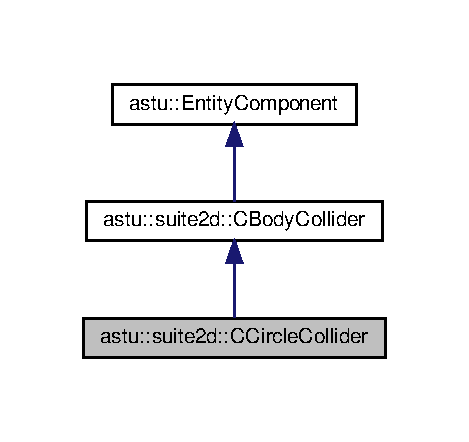
\includegraphics[width=225pt]{classastu_1_1suite2d_1_1CCircleCollider__inherit__graph}
\end{center}
\end{figure}


Collaboration diagram for astu\+:\+:suite2d\+:\+:C\+Circle\+Collider\+:\nopagebreak
\begin{figure}[H]
\begin{center}
\leavevmode
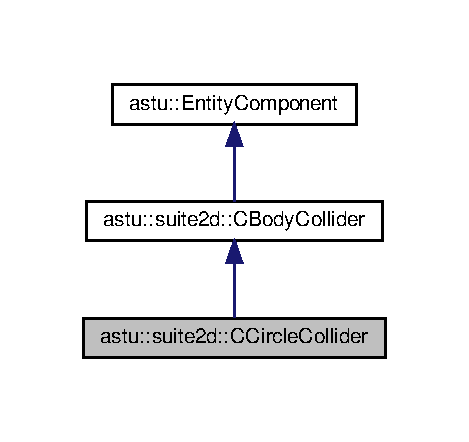
\includegraphics[width=225pt]{classastu_1_1suite2d_1_1CCircleCollider__coll__graph}
\end{center}
\end{figure}
\subsection*{Public Member Functions}
\begin{DoxyCompactItemize}
\item 
\hyperlink{classastu_1_1suite2d_1_1CCircleCollider_a724afec3b0f2b48e93bd0844bae5c951}{C\+Circle\+Collider} ()
\item 
float \hyperlink{classastu_1_1suite2d_1_1CCircleCollider_a7ec8a6c889a1502e9c650be905cd7aea}{Get\+Radius} () const
\item 
virtual void \hyperlink{classastu_1_1suite2d_1_1CCircleCollider_a0f064219591b23beace315bb58f26c78}{Set\+Radius} (float r)
\item 
virtual void \hyperlink{classastu_1_1suite2d_1_1CCircleCollider_aa77499480ca5f7d49f6331986b675a46}{On\+Added\+To\+Entity} (\hyperlink{classastu_1_1Entity}{Entity} \&entity)
\end{DoxyCompactItemize}


\subsection{Detailed Description}
Circular collider. 

\subsection{Constructor \& Destructor Documentation}
\mbox{\Hypertarget{classastu_1_1suite2d_1_1CCircleCollider_a724afec3b0f2b48e93bd0844bae5c951}\label{classastu_1_1suite2d_1_1CCircleCollider_a724afec3b0f2b48e93bd0844bae5c951}} 
\index{astu\+::suite2d\+::\+C\+Circle\+Collider@{astu\+::suite2d\+::\+C\+Circle\+Collider}!C\+Circle\+Collider@{C\+Circle\+Collider}}
\index{C\+Circle\+Collider@{C\+Circle\+Collider}!astu\+::suite2d\+::\+C\+Circle\+Collider@{astu\+::suite2d\+::\+C\+Circle\+Collider}}
\subsubsection{\texorpdfstring{C\+Circle\+Collider()}{CCircleCollider()}}
{\footnotesize\ttfamily astu\+::suite2d\+::\+C\+Circle\+Collider\+::\+C\+Circle\+Collider (\begin{DoxyParamCaption}{ }\end{DoxyParamCaption})\hspace{0.3cm}{\ttfamily [inline]}}

Constructor. 

\subsection{Member Function Documentation}
\mbox{\Hypertarget{classastu_1_1suite2d_1_1CCircleCollider_a7ec8a6c889a1502e9c650be905cd7aea}\label{classastu_1_1suite2d_1_1CCircleCollider_a7ec8a6c889a1502e9c650be905cd7aea}} 
\index{astu\+::suite2d\+::\+C\+Circle\+Collider@{astu\+::suite2d\+::\+C\+Circle\+Collider}!Get\+Radius@{Get\+Radius}}
\index{Get\+Radius@{Get\+Radius}!astu\+::suite2d\+::\+C\+Circle\+Collider@{astu\+::suite2d\+::\+C\+Circle\+Collider}}
\subsubsection{\texorpdfstring{Get\+Radius()}{GetRadius()}}
{\footnotesize\ttfamily float astu\+::suite2d\+::\+C\+Circle\+Collider\+::\+Get\+Radius (\begin{DoxyParamCaption}{ }\end{DoxyParamCaption}) const\hspace{0.3cm}{\ttfamily [inline]}}

Returns the radius of this circle collider.

\begin{DoxyReturn}{Returns}
the radius 
\end{DoxyReturn}
\mbox{\Hypertarget{classastu_1_1suite2d_1_1CCircleCollider_aa77499480ca5f7d49f6331986b675a46}\label{classastu_1_1suite2d_1_1CCircleCollider_aa77499480ca5f7d49f6331986b675a46}} 
\index{astu\+::suite2d\+::\+C\+Circle\+Collider@{astu\+::suite2d\+::\+C\+Circle\+Collider}!On\+Added\+To\+Entity@{On\+Added\+To\+Entity}}
\index{On\+Added\+To\+Entity@{On\+Added\+To\+Entity}!astu\+::suite2d\+::\+C\+Circle\+Collider@{astu\+::suite2d\+::\+C\+Circle\+Collider}}
\subsubsection{\texorpdfstring{On\+Added\+To\+Entity()}{OnAddedToEntity()}}
{\footnotesize\ttfamily virtual void astu\+::suite2d\+::\+C\+Circle\+Collider\+::\+On\+Added\+To\+Entity (\begin{DoxyParamCaption}\item[{\hyperlink{classastu_1_1Entity}{Entity} \&}]{entity }\end{DoxyParamCaption})\hspace{0.3cm}{\ttfamily [inline]}, {\ttfamily [virtual]}}

Called when added to an entity.

Most components do not need to override this method. Is is used occasionally to register additional interfaces a component implements. Registering implemented interfaces is necessary in order to make a component accessible via this interface and not just by the component type itself.


\begin{DoxyParams}{Parameters}
{\em entity} & the entity this component has been added to \\
\hline
\end{DoxyParams}


Reimplemented from \hyperlink{classastu_1_1EntityComponent_a8736f12dc9d2be7d2569408fc1040480}{astu\+::\+Entity\+Component}.

\mbox{\Hypertarget{classastu_1_1suite2d_1_1CCircleCollider_a0f064219591b23beace315bb58f26c78}\label{classastu_1_1suite2d_1_1CCircleCollider_a0f064219591b23beace315bb58f26c78}} 
\index{astu\+::suite2d\+::\+C\+Circle\+Collider@{astu\+::suite2d\+::\+C\+Circle\+Collider}!Set\+Radius@{Set\+Radius}}
\index{Set\+Radius@{Set\+Radius}!astu\+::suite2d\+::\+C\+Circle\+Collider@{astu\+::suite2d\+::\+C\+Circle\+Collider}}
\subsubsection{\texorpdfstring{Set\+Radius()}{SetRadius()}}
{\footnotesize\ttfamily virtual void astu\+::suite2d\+::\+C\+Circle\+Collider\+::\+Set\+Radius (\begin{DoxyParamCaption}\item[{float}]{r }\end{DoxyParamCaption})\hspace{0.3cm}{\ttfamily [inline]}, {\ttfamily [virtual]}}

Sets the radius of this circle collider.


\begin{DoxyParams}{Parameters}
{\em r} & the radius of this collider \\
\hline
\end{DoxyParams}

\begin{DoxyExceptions}{Exceptions}
{\em std\+::domain\+\_\+error} & in case the radius is less or equal zero \\
\hline
\end{DoxyExceptions}


The documentation for this class was generated from the following file\+:\begin{DoxyCompactItemize}
\item 
include/\+Suite2\+D/C\+Colliders.\+h\end{DoxyCompactItemize}

\hypertarget{classastu_1_1suite2d_1_1CCircleColliderBuilder}{}\section{astu\+:\+:suite2d\+:\+:C\+Circle\+Collider\+Builder Class Reference}
\label{classastu_1_1suite2d_1_1CCircleColliderBuilder}\index{astu\+::suite2d\+::\+C\+Circle\+Collider\+Builder@{astu\+::suite2d\+::\+C\+Circle\+Collider\+Builder}}


{\ttfamily \#include $<$C\+Colliders.\+h$>$}



Inheritance diagram for astu\+:\+:suite2d\+:\+:C\+Circle\+Collider\+Builder\+:\nopagebreak
\begin{figure}[H]
\begin{center}
\leavevmode
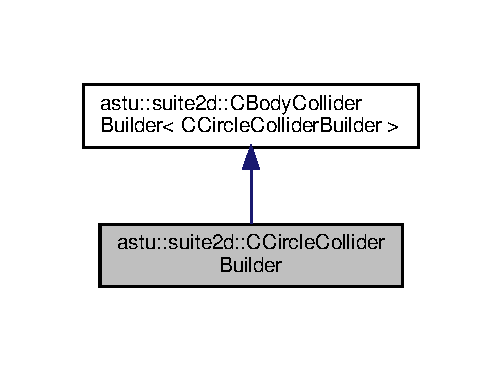
\includegraphics[width=241pt]{classastu_1_1suite2d_1_1CCircleColliderBuilder__inherit__graph}
\end{center}
\end{figure}


Collaboration diagram for astu\+:\+:suite2d\+:\+:C\+Circle\+Collider\+Builder\+:\nopagebreak
\begin{figure}[H]
\begin{center}
\leavevmode
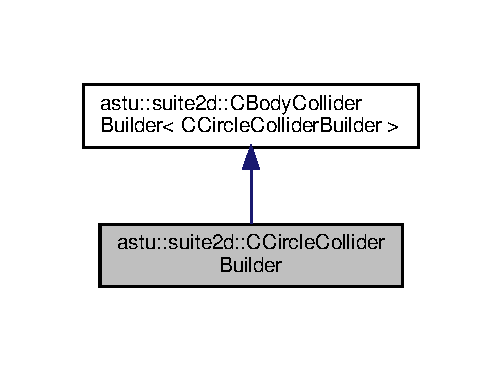
\includegraphics[width=241pt]{classastu_1_1suite2d_1_1CCircleColliderBuilder__coll__graph}
\end{center}
\end{figure}
\subsection*{Public Member Functions}
\begin{DoxyCompactItemize}
\item 
\hyperlink{classastu_1_1suite2d_1_1CCircleColliderBuilder_ad2a056e20fa1bb2ba7236125fc0a3aef}{C\+Circle\+Collider\+Builder} (std\+::shared\+\_\+ptr$<$ \hyperlink{classastu_1_1suite2d_1_1CCircleColliderFactory}{C\+Circle\+Collider\+Factory} $>$ collider\+Factory=nullptr)
\item 
\hyperlink{classastu_1_1suite2d_1_1CCircleColliderBuilder}{C\+Circle\+Collider\+Builder} \& \hyperlink{classastu_1_1suite2d_1_1CCircleColliderBuilder_ae75f2dcf4f2e99ed9ead657e661baa62}{Radius} (float r)
\item 
\hyperlink{classastu_1_1suite2d_1_1CCircleColliderBuilder}{C\+Circle\+Collider\+Builder} \& \hyperlink{classastu_1_1suite2d_1_1CCircleColliderBuilder_a0a946698baba5db84d97c648a79b224f}{Reset} ()
\item 
std\+::shared\+\_\+ptr$<$ \hyperlink{classastu_1_1suite2d_1_1CCircleCollider}{C\+Circle\+Collider} $>$ \hyperlink{classastu_1_1suite2d_1_1CCircleColliderBuilder_a50bb53e880b061f2040103cf8a1fe332}{Build} ()
\end{DoxyCompactItemize}
\subsection*{Additional Inherited Members}


\subsection{Detailed Description}
Builds \hyperlink{classastu_1_1suite2d_1_1CCircleCollider}{C\+Circle\+Collider} instances. 

\subsection{Constructor \& Destructor Documentation}
\mbox{\Hypertarget{classastu_1_1suite2d_1_1CCircleColliderBuilder_ad2a056e20fa1bb2ba7236125fc0a3aef}\label{classastu_1_1suite2d_1_1CCircleColliderBuilder_ad2a056e20fa1bb2ba7236125fc0a3aef}} 
\index{astu\+::suite2d\+::\+C\+Circle\+Collider\+Builder@{astu\+::suite2d\+::\+C\+Circle\+Collider\+Builder}!C\+Circle\+Collider\+Builder@{C\+Circle\+Collider\+Builder}}
\index{C\+Circle\+Collider\+Builder@{C\+Circle\+Collider\+Builder}!astu\+::suite2d\+::\+C\+Circle\+Collider\+Builder@{astu\+::suite2d\+::\+C\+Circle\+Collider\+Builder}}
\subsubsection{\texorpdfstring{C\+Circle\+Collider\+Builder()}{CCircleColliderBuilder()}}
{\footnotesize\ttfamily astu\+::suite2d\+::\+C\+Circle\+Collider\+Builder\+::\+C\+Circle\+Collider\+Builder (\begin{DoxyParamCaption}\item[{std\+::shared\+\_\+ptr$<$ \hyperlink{classastu_1_1suite2d_1_1CCircleColliderFactory}{C\+Circle\+Collider\+Factory} $>$}]{collider\+Factory = {\ttfamily nullptr} }\end{DoxyParamCaption})}

Constructor.

If the specified collider factory is null a service which implements the collider factory interface will be used.


\begin{DoxyParams}{Parameters}
{\em collider\+Factory} & the factory used to create new instances \\
\hline
\end{DoxyParams}


\subsection{Member Function Documentation}
\mbox{\Hypertarget{classastu_1_1suite2d_1_1CCircleColliderBuilder_a50bb53e880b061f2040103cf8a1fe332}\label{classastu_1_1suite2d_1_1CCircleColliderBuilder_a50bb53e880b061f2040103cf8a1fe332}} 
\index{astu\+::suite2d\+::\+C\+Circle\+Collider\+Builder@{astu\+::suite2d\+::\+C\+Circle\+Collider\+Builder}!Build@{Build}}
\index{Build@{Build}!astu\+::suite2d\+::\+C\+Circle\+Collider\+Builder@{astu\+::suite2d\+::\+C\+Circle\+Collider\+Builder}}
\subsubsection{\texorpdfstring{Build()}{Build()}}
{\footnotesize\ttfamily std\+::shared\+\_\+ptr$<$\hyperlink{classastu_1_1suite2d_1_1CCircleCollider}{C\+Circle\+Collider}$>$ astu\+::suite2d\+::\+C\+Circle\+Collider\+Builder\+::\+Build (\begin{DoxyParamCaption}{ }\end{DoxyParamCaption})}

Builds a new circle collider according to the current configuration.

\begin{DoxyReturn}{Returns}
the newly created circle collider 
\end{DoxyReturn}
\mbox{\Hypertarget{classastu_1_1suite2d_1_1CCircleColliderBuilder_ae75f2dcf4f2e99ed9ead657e661baa62}\label{classastu_1_1suite2d_1_1CCircleColliderBuilder_ae75f2dcf4f2e99ed9ead657e661baa62}} 
\index{astu\+::suite2d\+::\+C\+Circle\+Collider\+Builder@{astu\+::suite2d\+::\+C\+Circle\+Collider\+Builder}!Radius@{Radius}}
\index{Radius@{Radius}!astu\+::suite2d\+::\+C\+Circle\+Collider\+Builder@{astu\+::suite2d\+::\+C\+Circle\+Collider\+Builder}}
\subsubsection{\texorpdfstring{Radius()}{Radius()}}
{\footnotesize\ttfamily \hyperlink{classastu_1_1suite2d_1_1CCircleColliderBuilder}{C\+Circle\+Collider\+Builder}\& astu\+::suite2d\+::\+C\+Circle\+Collider\+Builder\+::\+Radius (\begin{DoxyParamCaption}\item[{float}]{r }\end{DoxyParamCaption})\hspace{0.3cm}{\ttfamily [inline]}}

Sets the radius of the circle collider to build.


\begin{DoxyParams}{Parameters}
{\em r} & the radius of the collider \\
\hline
\end{DoxyParams}

\begin{DoxyExceptions}{Exceptions}
{\em std\+::domain\+\_\+error} & in case the radius is less or equal zero \\
\hline
\end{DoxyExceptions}
\mbox{\Hypertarget{classastu_1_1suite2d_1_1CCircleColliderBuilder_a0a946698baba5db84d97c648a79b224f}\label{classastu_1_1suite2d_1_1CCircleColliderBuilder_a0a946698baba5db84d97c648a79b224f}} 
\index{astu\+::suite2d\+::\+C\+Circle\+Collider\+Builder@{astu\+::suite2d\+::\+C\+Circle\+Collider\+Builder}!Reset@{Reset}}
\index{Reset@{Reset}!astu\+::suite2d\+::\+C\+Circle\+Collider\+Builder@{astu\+::suite2d\+::\+C\+Circle\+Collider\+Builder}}
\subsubsection{\texorpdfstring{Reset()}{Reset()}}
{\footnotesize\ttfamily \hyperlink{classastu_1_1suite2d_1_1CCircleColliderBuilder}{C\+Circle\+Collider\+Builder}\& astu\+::suite2d\+::\+C\+Circle\+Collider\+Builder\+::\+Reset (\begin{DoxyParamCaption}{ }\end{DoxyParamCaption})\hspace{0.3cm}{\ttfamily [inline]}}

Resets this builder to its initial configuration.

\begin{DoxyReturn}{Returns}
reference to this builder for method chaining 
\end{DoxyReturn}


The documentation for this class was generated from the following file\+:\begin{DoxyCompactItemize}
\item 
include/\+Suite2\+D/C\+Colliders.\+h\end{DoxyCompactItemize}

\hypertarget{classastu_1_1suite2d_1_1CCircleColliderFactory}{}\section{astu\+:\+:suite2d\+:\+:C\+Circle\+Collider\+Factory Class Reference}
\label{classastu_1_1suite2d_1_1CCircleColliderFactory}\index{astu\+::suite2d\+::\+C\+Circle\+Collider\+Factory@{astu\+::suite2d\+::\+C\+Circle\+Collider\+Factory}}


{\ttfamily \#include $<$C\+Colliders.\+h$>$}

\subsection*{Public Member Functions}
\begin{DoxyCompactItemize}
\item 
virtual \hyperlink{classastu_1_1suite2d_1_1CCircleColliderFactory_a10c0323ae13665f12a91a8ec996dec12}{$\sim$\+C\+Circle\+Collider\+Factory} ()
\item 
virtual std\+::shared\+\_\+ptr$<$ \hyperlink{classastu_1_1suite2d_1_1CCircleCollider}{C\+Circle\+Collider} $>$ \hyperlink{classastu_1_1suite2d_1_1CCircleColliderFactory_aa6a5f8005c8674ad1262619f085f6583}{Create\+Circle\+Collider} ()=0
\end{DoxyCompactItemize}


\subsection{Detailed Description}
Abstract factory for for \hyperlink{classastu_1_1suite2d_1_1CCircleCollider}{C\+Circle\+Collider} components. 

\subsection{Constructor \& Destructor Documentation}
\mbox{\Hypertarget{classastu_1_1suite2d_1_1CCircleColliderFactory_a10c0323ae13665f12a91a8ec996dec12}\label{classastu_1_1suite2d_1_1CCircleColliderFactory_a10c0323ae13665f12a91a8ec996dec12}} 
\index{astu\+::suite2d\+::\+C\+Circle\+Collider\+Factory@{astu\+::suite2d\+::\+C\+Circle\+Collider\+Factory}!````~C\+Circle\+Collider\+Factory@{$\sim$\+C\+Circle\+Collider\+Factory}}
\index{````~C\+Circle\+Collider\+Factory@{$\sim$\+C\+Circle\+Collider\+Factory}!astu\+::suite2d\+::\+C\+Circle\+Collider\+Factory@{astu\+::suite2d\+::\+C\+Circle\+Collider\+Factory}}
\subsubsection{\texorpdfstring{$\sim$\+C\+Circle\+Collider\+Factory()}{~CCircleColliderFactory()}}
{\footnotesize\ttfamily virtual astu\+::suite2d\+::\+C\+Circle\+Collider\+Factory\+::$\sim$\+C\+Circle\+Collider\+Factory (\begin{DoxyParamCaption}{ }\end{DoxyParamCaption})\hspace{0.3cm}{\ttfamily [inline]}, {\ttfamily [virtual]}}

Virtual destructor. 

\subsection{Member Function Documentation}
\mbox{\Hypertarget{classastu_1_1suite2d_1_1CCircleColliderFactory_aa6a5f8005c8674ad1262619f085f6583}\label{classastu_1_1suite2d_1_1CCircleColliderFactory_aa6a5f8005c8674ad1262619f085f6583}} 
\index{astu\+::suite2d\+::\+C\+Circle\+Collider\+Factory@{astu\+::suite2d\+::\+C\+Circle\+Collider\+Factory}!Create\+Circle\+Collider@{Create\+Circle\+Collider}}
\index{Create\+Circle\+Collider@{Create\+Circle\+Collider}!astu\+::suite2d\+::\+C\+Circle\+Collider\+Factory@{astu\+::suite2d\+::\+C\+Circle\+Collider\+Factory}}
\subsubsection{\texorpdfstring{Create\+Circle\+Collider()}{CreateCircleCollider()}}
{\footnotesize\ttfamily virtual std\+::shared\+\_\+ptr$<$\hyperlink{classastu_1_1suite2d_1_1CCircleCollider}{C\+Circle\+Collider}$>$ astu\+::suite2d\+::\+C\+Circle\+Collider\+Factory\+::\+Create\+Circle\+Collider (\begin{DoxyParamCaption}{ }\end{DoxyParamCaption})\hspace{0.3cm}{\ttfamily [pure virtual]}}

Creates a new \hyperlink{classastu_1_1suite2d_1_1CCircleCollider}{C\+Circle\+Collider} instance. 

The documentation for this class was generated from the following file\+:\begin{DoxyCompactItemize}
\item 
include/\+Suite2\+D/C\+Colliders.\+h\end{DoxyCompactItemize}

\hypertarget{classastu_1_1suite2d_1_1CollisionListener}{}\section{astu\+:\+:suite2d\+:\+:Collision\+Listener Class Reference}
\label{classastu_1_1suite2d_1_1CollisionListener}\index{astu\+::suite2d\+::\+Collision\+Listener@{astu\+::suite2d\+::\+Collision\+Listener}}


{\ttfamily \#include $<$Collision\+Signal.\+h$>$}



Inheritance diagram for astu\+:\+:suite2d\+:\+:Collision\+Listener\+:\nopagebreak
\begin{figure}[H]
\begin{center}
\leavevmode
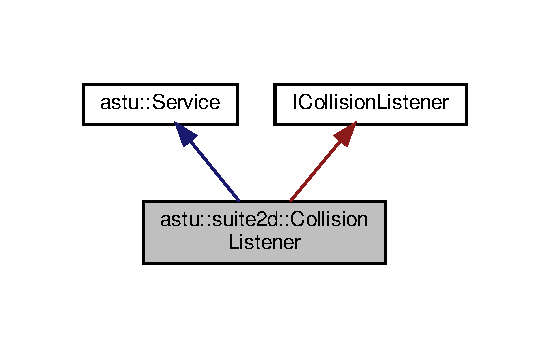
\includegraphics[width=264pt]{classastu_1_1suite2d_1_1CollisionListener__inherit__graph}
\end{center}
\end{figure}


Collaboration diagram for astu\+:\+:suite2d\+:\+:Collision\+Listener\+:\nopagebreak
\begin{figure}[H]
\begin{center}
\leavevmode
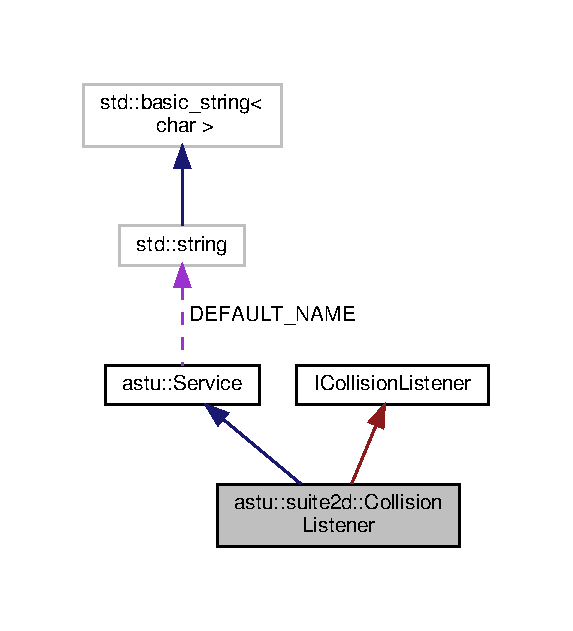
\includegraphics[width=275pt]{classastu_1_1suite2d_1_1CollisionListener__coll__graph}
\end{center}
\end{figure}
\subsection*{Public Member Functions}
\begin{DoxyCompactItemize}
\item 
\hyperlink{classastu_1_1suite2d_1_1CollisionListener_ac8450939232e333a3f3de7b8f0a08fd7}{Collision\+Listener} ()
\end{DoxyCompactItemize}
\subsection*{Protected Member Functions}
\begin{DoxyCompactItemize}
\item 
virtual bool \hyperlink{classastu_1_1suite2d_1_1CollisionListener_a784ca22e86d659d042aaab818c488a56}{On\+Collision} (\hyperlink{classastu_1_1Entity}{astu\+::\+Entity} \&entityA, \hyperlink{classastu_1_1Entity}{astu\+::\+Entity} \&entityB)
\end{DoxyCompactItemize}
\subsection*{Additional Inherited Members}


\subsection{Detailed Description}
Services can derive from this class to process mouse wheel signals. 

\subsection{Constructor \& Destructor Documentation}
\mbox{\Hypertarget{classastu_1_1suite2d_1_1CollisionListener_ac8450939232e333a3f3de7b8f0a08fd7}\label{classastu_1_1suite2d_1_1CollisionListener_ac8450939232e333a3f3de7b8f0a08fd7}} 
\index{astu\+::suite2d\+::\+Collision\+Listener@{astu\+::suite2d\+::\+Collision\+Listener}!Collision\+Listener@{Collision\+Listener}}
\index{Collision\+Listener@{Collision\+Listener}!astu\+::suite2d\+::\+Collision\+Listener@{astu\+::suite2d\+::\+Collision\+Listener}}
\subsubsection{\texorpdfstring{Collision\+Listener()}{CollisionListener()}}
{\footnotesize\ttfamily astu\+::suite2d\+::\+Collision\+Listener\+::\+Collision\+Listener (\begin{DoxyParamCaption}{ }\end{DoxyParamCaption})\hspace{0.3cm}{\ttfamily [inline]}}

Constructor. 

\subsection{Member Function Documentation}
\mbox{\Hypertarget{classastu_1_1suite2d_1_1CollisionListener_a784ca22e86d659d042aaab818c488a56}\label{classastu_1_1suite2d_1_1CollisionListener_a784ca22e86d659d042aaab818c488a56}} 
\index{astu\+::suite2d\+::\+Collision\+Listener@{astu\+::suite2d\+::\+Collision\+Listener}!On\+Collision@{On\+Collision}}
\index{On\+Collision@{On\+Collision}!astu\+::suite2d\+::\+Collision\+Listener@{astu\+::suite2d\+::\+Collision\+Listener}}
\subsubsection{\texorpdfstring{On\+Collision()}{OnCollision()}}
{\footnotesize\ttfamily virtual bool astu\+::suite2d\+::\+Collision\+Listener\+::\+On\+Collision (\begin{DoxyParamCaption}\item[{\hyperlink{classastu_1_1Entity}{astu\+::\+Entity} \&}]{entityA,  }\item[{\hyperlink{classastu_1_1Entity}{astu\+::\+Entity} \&}]{entityB }\end{DoxyParamCaption})\hspace{0.3cm}{\ttfamily [inline]}, {\ttfamily [protected]}, {\ttfamily [virtual]}}

Called by this base class when a collision event has been received


\begin{DoxyParams}{Parameters}
{\em entityA} & the first entity \\
\hline
{\em entityB} & the second entity \\
\hline
\end{DoxyParams}


The documentation for this class was generated from the following file\+:\begin{DoxyCompactItemize}
\item 
include/\+Suite2\+D/Collision\+Signal.\+h\end{DoxyCompactItemize}

\hypertarget{classastu_1_1suite2d_1_1CollisionSignal}{}\section{astu\+:\+:suite2d\+:\+:Collision\+Signal Class Reference}
\label{classastu_1_1suite2d_1_1CollisionSignal}\index{astu\+::suite2d\+::\+Collision\+Signal@{astu\+::suite2d\+::\+Collision\+Signal}}


{\ttfamily \#include $<$Collision\+Signal.\+h$>$}

\subsection*{Public Member Functions}
\begin{DoxyCompactItemize}
\item 
\hyperlink{classastu_1_1suite2d_1_1CollisionSignal_a415a7bde99513f42d1192bf07c3afd5c}{Collision\+Signal} (std\+::shared\+\_\+ptr$<$ \hyperlink{classastu_1_1Entity}{astu\+::\+Entity} $>$ a, std\+::shared\+\_\+ptr$<$ \hyperlink{classastu_1_1Entity}{astu\+::\+Entity} $>$ b)
\end{DoxyCompactItemize}
\subsection*{Public Attributes}
\begin{DoxyCompactItemize}
\item 
std\+::shared\+\_\+ptr$<$ \hyperlink{classastu_1_1Entity}{astu\+::\+Entity} $>$ \hyperlink{classastu_1_1suite2d_1_1CollisionSignal_a7ace89d8dca0c0b38e74d8bd04ecead1}{entityA}
\item 
std\+::shared\+\_\+ptr$<$ \hyperlink{classastu_1_1Entity}{astu\+::\+Entity} $>$ \hyperlink{classastu_1_1suite2d_1_1CollisionSignal_a5a68c5c6df677411bcc8a30a1df8b53b}{entityB}
\end{DoxyCompactItemize}


\subsection{Detailed Description}
This signal represents a collision between two entities. 

\subsection{Constructor \& Destructor Documentation}
\mbox{\Hypertarget{classastu_1_1suite2d_1_1CollisionSignal_a415a7bde99513f42d1192bf07c3afd5c}\label{classastu_1_1suite2d_1_1CollisionSignal_a415a7bde99513f42d1192bf07c3afd5c}} 
\index{astu\+::suite2d\+::\+Collision\+Signal@{astu\+::suite2d\+::\+Collision\+Signal}!Collision\+Signal@{Collision\+Signal}}
\index{Collision\+Signal@{Collision\+Signal}!astu\+::suite2d\+::\+Collision\+Signal@{astu\+::suite2d\+::\+Collision\+Signal}}
\subsubsection{\texorpdfstring{Collision\+Signal()}{CollisionSignal()}}
{\footnotesize\ttfamily astu\+::suite2d\+::\+Collision\+Signal\+::\+Collision\+Signal (\begin{DoxyParamCaption}\item[{std\+::shared\+\_\+ptr$<$ \hyperlink{classastu_1_1Entity}{astu\+::\+Entity} $>$}]{a,  }\item[{std\+::shared\+\_\+ptr$<$ \hyperlink{classastu_1_1Entity}{astu\+::\+Entity} $>$}]{b }\end{DoxyParamCaption})\hspace{0.3cm}{\ttfamily [inline]}}

Constructor.


\begin{DoxyParams}{Parameters}
{\em a} & the first entity \\
\hline
{\em b} & the second entity \\
\hline
\end{DoxyParams}


\subsection{Member Data Documentation}
\mbox{\Hypertarget{classastu_1_1suite2d_1_1CollisionSignal_a7ace89d8dca0c0b38e74d8bd04ecead1}\label{classastu_1_1suite2d_1_1CollisionSignal_a7ace89d8dca0c0b38e74d8bd04ecead1}} 
\index{astu\+::suite2d\+::\+Collision\+Signal@{astu\+::suite2d\+::\+Collision\+Signal}!entityA@{entityA}}
\index{entityA@{entityA}!astu\+::suite2d\+::\+Collision\+Signal@{astu\+::suite2d\+::\+Collision\+Signal}}
\subsubsection{\texorpdfstring{entityA}{entityA}}
{\footnotesize\ttfamily std\+::shared\+\_\+ptr$<$\hyperlink{classastu_1_1Entity}{astu\+::\+Entity}$>$ astu\+::suite2d\+::\+Collision\+Signal\+::entityA}

The first entity involved in the collision. \mbox{\Hypertarget{classastu_1_1suite2d_1_1CollisionSignal_a5a68c5c6df677411bcc8a30a1df8b53b}\label{classastu_1_1suite2d_1_1CollisionSignal_a5a68c5c6df677411bcc8a30a1df8b53b}} 
\index{astu\+::suite2d\+::\+Collision\+Signal@{astu\+::suite2d\+::\+Collision\+Signal}!entityB@{entityB}}
\index{entityB@{entityB}!astu\+::suite2d\+::\+Collision\+Signal@{astu\+::suite2d\+::\+Collision\+Signal}}
\subsubsection{\texorpdfstring{entityB}{entityB}}
{\footnotesize\ttfamily std\+::shared\+\_\+ptr$<$\hyperlink{classastu_1_1Entity}{astu\+::\+Entity}$>$ astu\+::suite2d\+::\+Collision\+Signal\+::entityB}

The second entity involved in the collision. 

The documentation for this class was generated from the following file\+:\begin{DoxyCompactItemize}
\item 
include/\+Suite2\+D/Collision\+Signal.\+h\end{DoxyCompactItemize}

\hypertarget{classastu_1_1Color}{}\section{astu\+:\+:Color$<$ T $>$ Class Template Reference}
\label{classastu_1_1Color}\index{astu\+::\+Color$<$ T $>$@{astu\+::\+Color$<$ T $>$}}


{\ttfamily \#include $<$Color.\+h$>$}



Collaboration diagram for astu\+:\+:Color$<$ T $>$\+:\nopagebreak
\begin{figure}[H]
\begin{center}
\leavevmode
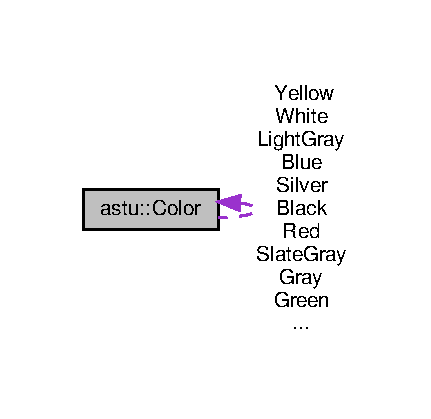
\includegraphics[width=169pt]{classastu_1_1Color__coll__graph}
\end{center}
\end{figure}
\subsection*{Public Member Functions}
\begin{DoxyCompactItemize}
\item 
\hyperlink{classastu_1_1Color_abb0e2cdad572357375d5b2465ea847b9}{Color} (T red=0, T green=0, T blue=0, T alpha=1)
\item 
\hyperlink{classastu_1_1Color_a1ce283cfd9542b85da611fc50a4a9e54}{Color} (int rgb)
\item 
\hyperlink{classastu_1_1Color}{Color}$<$ T $>$ \& \hyperlink{classastu_1_1Color_a0fcfa896c3a32ae0af1aeec3f4d866fe}{Set\+Alpha} (T \hyperlink{classastu_1_1Color_ad62b3af3464dea4bf99432bfb6e9d796}{a})
\item 
void \hyperlink{classastu_1_1Color_ad5aaf54919fed257c37b6b5747bd01c8}{Set} (T red, T green, T blue, T alpha=1)
\item 
int \hyperlink{classastu_1_1Color_a376a9d08b37e917a7040d58aab009bf5}{To\+Rgba} () const
\item 
T \hyperlink{classastu_1_1Color_a4802f8f0d0fcf65ba6853ac17c52b811}{Distance\+Without\+Alpha} (const \hyperlink{classastu_1_1Color}{Color}$<$ T $>$ \&o) const
\item 
T \hyperlink{classastu_1_1Color_a35549a6d06ab1fbc8a232508e3041f9d}{Distance\+Squared\+Without\+Alpha} (const \hyperlink{classastu_1_1Color}{Color}$<$ T $>$ \&o) const
\item 
T \hyperlink{classastu_1_1Color_aa61d12089e02ec0ce02ab877b21c6bcc}{Distance} (const \hyperlink{classastu_1_1Color}{Color}$<$ T $>$ \&o) const
\item 
T \hyperlink{classastu_1_1Color_a9b396fa9b0d3612ec9eb372b52de1eac}{Distance\+Squared} (const \hyperlink{classastu_1_1Color}{Color}$<$ T $>$ \&o) const
\item 
\hyperlink{classastu_1_1Color}{Color}$<$ T $>$ \& \hyperlink{classastu_1_1Color_a662946707019ddc5d79612da685be5f8}{Multiply\+Without\+Alpha} (T s) noexcept
\item 
int \hyperlink{classastu_1_1Color_aa7c679fe7a6c4b11ea163bc1d64fd73b}{Get\+A\+R\+GB} () const
\item 
int \hyperlink{classastu_1_1Color_a11cf3e00ee1662cc67aae0fa5767df39}{Get\+A\+B\+GR} () const
\item 
\hyperlink{classastu_1_1Color}{Color}$<$ T $>$ \& \hyperlink{classastu_1_1Color_a60780325071ef6c95b113f9f5f9905b4}{Saturate} () noexcept
\item 
\hyperlink{classastu_1_1Color}{Color}$<$ T $>$ \& \hyperlink{classastu_1_1Color_a33b9d43c6d2306ccd7e3071e0e52eb25}{Blend} (const \hyperlink{classastu_1_1Color}{Color}$<$ T $>$ \&o)
\item 
\hyperlink{classastu_1_1Color}{Color}$<$ T $>$ \hyperlink{classastu_1_1Color_acc63e1fac50adf874fa5b33516186e7f}{Lerp} (const \hyperlink{classastu_1_1Color}{Color}$<$ T $>$ \&o, T t) const
\item 
\hyperlink{classastu_1_1Color}{Color}$<$ T $>$ \hyperlink{classastu_1_1Color_a7f1c0093d51c4036f7ab5755d571d6e7}{operator+} (const \hyperlink{classastu_1_1Color}{Color}$<$ T $>$ \&rhs) const
\item 
\hyperlink{classastu_1_1Color}{Color}$<$ T $>$ \& \hyperlink{classastu_1_1Color_ab4cafbc5cbd4aa28a8feb428107d3985}{operator+=} (const \hyperlink{classastu_1_1Color}{Color}$<$ T $>$ \&rhs)
\item 
\hyperlink{classastu_1_1Color}{Color}$<$ T $>$ \hyperlink{classastu_1_1Color_a2d512332791d4187ecde51771648cb9c}{operator-\/} (const \hyperlink{classastu_1_1Color}{Color}$<$ T $>$ \&rhs) const
\item 
\hyperlink{classastu_1_1Color}{Color}$<$ T $>$ \& \hyperlink{classastu_1_1Color_add622a013366f3f07eee482493c2c158}{operator-\/=} (const \hyperlink{classastu_1_1Color}{Color}$<$ T $>$ \&rhs)
\item 
\hyperlink{classastu_1_1Color}{Color}$<$ T $>$ \hyperlink{classastu_1_1Color_aa1fc446d899409058a6e510775ae009d}{operator$\ast$} (T s) const
\item 
\hyperlink{classastu_1_1Color}{Color}$<$ T $>$ \& \hyperlink{classastu_1_1Color_ab097615260001619304f4d128b484359}{operator$\ast$=} (T s)
\item 
\hyperlink{classastu_1_1Color}{Color}$<$ T $>$ \hyperlink{classastu_1_1Color_af4b143f6c4c3b15412293a25f05320b2}{operator/} (T s) const
\item 
\hyperlink{classastu_1_1Color}{Color}$<$ T $>$ \& \hyperlink{classastu_1_1Color_a8411cf3d645429dbcdc609a8db010c68}{operator/=} (T s)
\item 
bool \hyperlink{classastu_1_1Color_a3cfd5f7a4157b012c4ca1df92289e525}{operator==} (const \hyperlink{classastu_1_1Color}{Color}$<$ T $>$ \&o) const
\item 
bool \hyperlink{classastu_1_1Color_a03214300c75b0737cd91679f758112c5}{operator!=} (const \hyperlink{classastu_1_1Color}{Color}$<$ T $>$ \&o) const
\item 
bool \hyperlink{classastu_1_1Color_a3ff28065c93ca64d4806186118eef206}{operator$<$} (const \hyperlink{classastu_1_1Color}{Color}$<$ T $>$ \&rhs) const
\end{DoxyCompactItemize}
\subsection*{Static Public Member Functions}
\begin{DoxyCompactItemize}
\item 
static \hyperlink{classastu_1_1Color}{Color}$<$ T $>$ \hyperlink{classastu_1_1Color_a02abdb3a0d65626cb6bae8cbad7d6dfd}{Create\+From\+Rgb} (int red, int green, int blue, int alpha=255)
\end{DoxyCompactItemize}
\subsection*{Public Attributes}
\begin{DoxyCompactItemize}
\item 
T \hyperlink{classastu_1_1Color_aa670f74822e1db4513844dca52b1eb6a}{r}
\item 
T \hyperlink{classastu_1_1Color_a3134881dda38a8f123387faeff309dff}{g}
\item 
T \hyperlink{classastu_1_1Color_a56d075e69ca5e4cea336f3977b04dee2}{b}
\item 
T \hyperlink{classastu_1_1Color_ad62b3af3464dea4bf99432bfb6e9d796}{a}
\end{DoxyCompactItemize}


\subsection{Detailed Description}
\subsubsection*{template$<$typename T$>$\newline
class astu\+::\+Color$<$ T $>$}

Represents a color value in R\+GB color space.

A color is described using four color channels\+: red, green, blue and alpha. The alpha channel represents transparency. The color channels are represents as floating-\/point values which normally lie within the interval \mbox{[}0, 1\mbox{]}. 

\subsection{Constructor \& Destructor Documentation}
\mbox{\Hypertarget{classastu_1_1Color_abb0e2cdad572357375d5b2465ea847b9}\label{classastu_1_1Color_abb0e2cdad572357375d5b2465ea847b9}} 
\index{astu\+::\+Color@{astu\+::\+Color}!Color@{Color}}
\index{Color@{Color}!astu\+::\+Color@{astu\+::\+Color}}
\subsubsection{\texorpdfstring{Color()}{Color()}\hspace{0.1cm}{\footnotesize\ttfamily [1/2]}}
{\footnotesize\ttfamily template$<$typename T$>$ \\
\hyperlink{classastu_1_1Color}{astu\+::\+Color}$<$ T $>$\+::\hyperlink{classastu_1_1Color}{Color} (\begin{DoxyParamCaption}\item[{T}]{red = {\ttfamily 0},  }\item[{T}]{green = {\ttfamily 0},  }\item[{T}]{blue = {\ttfamily 0},  }\item[{T}]{alpha = {\ttfamily 1} }\end{DoxyParamCaption})\hspace{0.3cm}{\ttfamily [inline]}}

Constructor.


\begin{DoxyParams}{Parameters}
{\em red} & the red color component \\
\hline
{\em green} & the green color component \\
\hline
{\em blue} & the blue color component \\
\hline
{\em alpha} & the alpha color component \\
\hline
\end{DoxyParams}
\mbox{\Hypertarget{classastu_1_1Color_a1ce283cfd9542b85da611fc50a4a9e54}\label{classastu_1_1Color_a1ce283cfd9542b85da611fc50a4a9e54}} 
\index{astu\+::\+Color@{astu\+::\+Color}!Color@{Color}}
\index{Color@{Color}!astu\+::\+Color@{astu\+::\+Color}}
\subsubsection{\texorpdfstring{Color()}{Color()}\hspace{0.1cm}{\footnotesize\ttfamily [2/2]}}
{\footnotesize\ttfamily template$<$typename T$>$ \\
\hyperlink{classastu_1_1Color}{astu\+::\+Color}$<$ T $>$\+::\hyperlink{classastu_1_1Color}{Color} (\begin{DoxyParamCaption}\item[{int}]{rgb }\end{DoxyParamCaption})\hspace{0.3cm}{\ttfamily [inline]}}

Constructor.

This constructor can be used to create colors using the usual hex-\/triplet notation which is a six-\/digit, three-\/byte hexadecimal number used int H\+T\+ML, C\+SS, S\+VG etc.

{\bfseries Example}


\begin{DoxyCode}
\hyperlink{classastu_1_1Color_abb0e2cdad572357375d5b2465ea847b9}{Color} mediumAquamarine(0x66cdaa);
\end{DoxyCode}


The enum \hyperlink{classastu_1_1WebColors}{Web\+Colors} defines integer constants according to the color names defined by the W3C standards. These constants can be used to initialize colors using this constructor.


\begin{DoxyCode}
\hyperlink{classastu_1_1Color_abb0e2cdad572357375d5b2465ea847b9}{Color} redColor(\hyperlink{classastu_1_1WebColors_ac75482e858498b1b3fa521ba93fcda98a56bb31647b5e647e11d2941f54a30781}{WebColors::Red});
\hyperlink{classastu_1_1Color_abb0e2cdad572357375d5b2465ea847b9}{Color} PurpleColor(\hyperlink{classastu_1_1WebColors_ac75482e858498b1b3fa521ba93fcda98a3d63297abeb7cf60c2ddae0a1ee3e658}{WebColors::Purple});
\end{DoxyCode}


This constructor also functions as automatic conversion constructor which allows C++ to automatically convert integers to objects of class \hyperlink{classastu_1_1Color}{Color}. This makes it particularly easy to use the Web\+Color constants to initialize colors\+:


\begin{DoxyCode}
\hyperlink{classastu_1_1Color_abb0e2cdad572357375d5b2465ea847b9}{Color} redColor = \hyperlink{classastu_1_1WebColors_ac75482e858498b1b3fa521ba93fcda98a56bb31647b5e647e11d2941f54a30781}{WebColors::Red};
\end{DoxyCode}


or even as function arguments of type color


\begin{DoxyCode}
\textcolor{preprocessor}{#include <Color.h>}

\textcolor{keywordtype}{void} SomeFunction(\textcolor{keyword}{const} \hyperlink{classastu_1_1Color_abb0e2cdad572357375d5b2465ea847b9}{Color} & c) \{
 \textcolor{comment}{// Does something with c...}
\}

\textcolor{keywordtype}{int} main() \{
  SomeFunction(\hyperlink{classastu_1_1WebColors_ac75482e858498b1b3fa521ba93fcda98a93a4bd8dbcd8c09329c7d866c835571c}{WebColors::Aqua});

  \textcolor{keywordflow}{return} 0;
\}
\end{DoxyCode}



\begin{DoxyParams}{Parameters}
{\em rgb} & the rgb color components encoded within in an integer \\
\hline
\end{DoxyParams}


\subsection{Member Function Documentation}
\mbox{\Hypertarget{classastu_1_1Color_a33b9d43c6d2306ccd7e3071e0e52eb25}\label{classastu_1_1Color_a33b9d43c6d2306ccd7e3071e0e52eb25}} 
\index{astu\+::\+Color@{astu\+::\+Color}!Blend@{Blend}}
\index{Blend@{Blend}!astu\+::\+Color@{astu\+::\+Color}}
\subsubsection{\texorpdfstring{Blend()}{Blend()}}
{\footnotesize\ttfamily template$<$typename T$>$ \\
\hyperlink{classastu_1_1Color}{Color}$<$T$>$\& \hyperlink{classastu_1_1Color}{astu\+::\+Color}$<$ T $>$\+::Blend (\begin{DoxyParamCaption}\item[{const \hyperlink{classastu_1_1Color}{Color}$<$ T $>$ \&}]{o }\end{DoxyParamCaption})\hspace{0.3cm}{\ttfamily [inline]}}

Blends this color with another color respecting the alpha channel.

This method changes this color and leaves the other color untouched, which is the most common usage of this method.


\begin{DoxyParams}{Parameters}
{\em o} & the other color to blend with this color \\
\hline
\end{DoxyParams}
\begin{DoxyReturn}{Returns}
a reference to this color used for method chaining 
\end{DoxyReturn}
\mbox{\Hypertarget{classastu_1_1Color_a02abdb3a0d65626cb6bae8cbad7d6dfd}\label{classastu_1_1Color_a02abdb3a0d65626cb6bae8cbad7d6dfd}} 
\index{astu\+::\+Color@{astu\+::\+Color}!Create\+From\+Rgb@{Create\+From\+Rgb}}
\index{Create\+From\+Rgb@{Create\+From\+Rgb}!astu\+::\+Color@{astu\+::\+Color}}
\subsubsection{\texorpdfstring{Create\+From\+Rgb()}{CreateFromRgb()}}
{\footnotesize\ttfamily template$<$typename T$>$ \\
static \hyperlink{classastu_1_1Color}{Color}$<$T$>$ \hyperlink{classastu_1_1Color}{astu\+::\+Color}$<$ T $>$\+::Create\+From\+Rgb (\begin{DoxyParamCaption}\item[{int}]{red,  }\item[{int}]{green,  }\item[{int}]{blue,  }\item[{int}]{alpha = {\ttfamily 255} }\end{DoxyParamCaption})\hspace{0.3cm}{\ttfamily [inline]}, {\ttfamily [static]}}

Creates a color from R\+GB integer values.


\begin{DoxyParams}{Parameters}
{\em red} & red color component, value within the range 0 and 255 \\
\hline
{\em green} & green color component, value within the range 0 and 255 \\
\hline
{\em blue} & blue color component, value within the range 0 and 255 \\
\hline
{\em alpha} & transparency, value within the range 0 and 255 \\
\hline
\end{DoxyParams}
\mbox{\Hypertarget{classastu_1_1Color_aa61d12089e02ec0ce02ab877b21c6bcc}\label{classastu_1_1Color_aa61d12089e02ec0ce02ab877b21c6bcc}} 
\index{astu\+::\+Color@{astu\+::\+Color}!Distance@{Distance}}
\index{Distance@{Distance}!astu\+::\+Color@{astu\+::\+Color}}
\subsubsection{\texorpdfstring{Distance()}{Distance()}}
{\footnotesize\ttfamily template$<$typename T$>$ \\
T \hyperlink{classastu_1_1Color}{astu\+::\+Color}$<$ T $>$\+::Distance (\begin{DoxyParamCaption}\item[{const \hyperlink{classastu_1_1Color}{Color}$<$ T $>$ \&}]{o }\end{DoxyParamCaption}) const\hspace{0.3cm}{\ttfamily [inline]}}

Calculates the Euclidean in R\+G\+BA color space.


\begin{DoxyParams}{Parameters}
{\em o} & the other color \\
\hline
\end{DoxyParams}
\begin{DoxyReturn}{Returns}
the distance to the other color 
\end{DoxyReturn}
\mbox{\Hypertarget{classastu_1_1Color_a9b396fa9b0d3612ec9eb372b52de1eac}\label{classastu_1_1Color_a9b396fa9b0d3612ec9eb372b52de1eac}} 
\index{astu\+::\+Color@{astu\+::\+Color}!Distance\+Squared@{Distance\+Squared}}
\index{Distance\+Squared@{Distance\+Squared}!astu\+::\+Color@{astu\+::\+Color}}
\subsubsection{\texorpdfstring{Distance\+Squared()}{DistanceSquared()}}
{\footnotesize\ttfamily template$<$typename T$>$ \\
T \hyperlink{classastu_1_1Color}{astu\+::\+Color}$<$ T $>$\+::Distance\+Squared (\begin{DoxyParamCaption}\item[{const \hyperlink{classastu_1_1Color}{Color}$<$ T $>$ \&}]{o }\end{DoxyParamCaption}) const\hspace{0.3cm}{\ttfamily [inline]}}

Calculates the Euclidean squared in R\+G\+BA color space.


\begin{DoxyParams}{Parameters}
{\em o} & the other color \\
\hline
\end{DoxyParams}
\begin{DoxyReturn}{Returns}
the distance to the other color 
\end{DoxyReturn}
\mbox{\Hypertarget{classastu_1_1Color_a35549a6d06ab1fbc8a232508e3041f9d}\label{classastu_1_1Color_a35549a6d06ab1fbc8a232508e3041f9d}} 
\index{astu\+::\+Color@{astu\+::\+Color}!Distance\+Squared\+Without\+Alpha@{Distance\+Squared\+Without\+Alpha}}
\index{Distance\+Squared\+Without\+Alpha@{Distance\+Squared\+Without\+Alpha}!astu\+::\+Color@{astu\+::\+Color}}
\subsubsection{\texorpdfstring{Distance\+Squared\+Without\+Alpha()}{DistanceSquaredWithoutAlpha()}}
{\footnotesize\ttfamily template$<$typename T$>$ \\
T \hyperlink{classastu_1_1Color}{astu\+::\+Color}$<$ T $>$\+::Distance\+Squared\+Without\+Alpha (\begin{DoxyParamCaption}\item[{const \hyperlink{classastu_1_1Color}{Color}$<$ T $>$ \&}]{o }\end{DoxyParamCaption}) const\hspace{0.3cm}{\ttfamily [inline]}}

Calculates the Euclidean squared in R\+GB color space.


\begin{DoxyParams}{Parameters}
{\em o} & the other color \\
\hline
\end{DoxyParams}
\begin{DoxyReturn}{Returns}
the distance to the other color 
\end{DoxyReturn}
\mbox{\Hypertarget{classastu_1_1Color_a4802f8f0d0fcf65ba6853ac17c52b811}\label{classastu_1_1Color_a4802f8f0d0fcf65ba6853ac17c52b811}} 
\index{astu\+::\+Color@{astu\+::\+Color}!Distance\+Without\+Alpha@{Distance\+Without\+Alpha}}
\index{Distance\+Without\+Alpha@{Distance\+Without\+Alpha}!astu\+::\+Color@{astu\+::\+Color}}
\subsubsection{\texorpdfstring{Distance\+Without\+Alpha()}{DistanceWithoutAlpha()}}
{\footnotesize\ttfamily template$<$typename T$>$ \\
T \hyperlink{classastu_1_1Color}{astu\+::\+Color}$<$ T $>$\+::Distance\+Without\+Alpha (\begin{DoxyParamCaption}\item[{const \hyperlink{classastu_1_1Color}{Color}$<$ T $>$ \&}]{o }\end{DoxyParamCaption}) const\hspace{0.3cm}{\ttfamily [inline]}}

Calculates the Euclidean distance in R\+GB color space.


\begin{DoxyParams}{Parameters}
{\em o} & the other color \\
\hline
\end{DoxyParams}
\begin{DoxyReturn}{Returns}
the distance to the other color 
\end{DoxyReturn}
\mbox{\Hypertarget{classastu_1_1Color_a11cf3e00ee1662cc67aae0fa5767df39}\label{classastu_1_1Color_a11cf3e00ee1662cc67aae0fa5767df39}} 
\index{astu\+::\+Color@{astu\+::\+Color}!Get\+A\+B\+GR@{Get\+A\+B\+GR}}
\index{Get\+A\+B\+GR@{Get\+A\+B\+GR}!astu\+::\+Color@{astu\+::\+Color}}
\subsubsection{\texorpdfstring{Get\+A\+B\+G\+R()}{GetABGR()}}
{\footnotesize\ttfamily template$<$typename T$>$ \\
int \hyperlink{classastu_1_1Color}{astu\+::\+Color}$<$ T $>$\+::Get\+A\+B\+GR (\begin{DoxyParamCaption}{ }\end{DoxyParamCaption}) const\hspace{0.3cm}{\ttfamily [inline]}}

Converts this color to an integer value.

\begin{DoxyReturn}{Returns}
the integer representation of this color 
\end{DoxyReturn}
\mbox{\Hypertarget{classastu_1_1Color_aa7c679fe7a6c4b11ea163bc1d64fd73b}\label{classastu_1_1Color_aa7c679fe7a6c4b11ea163bc1d64fd73b}} 
\index{astu\+::\+Color@{astu\+::\+Color}!Get\+A\+R\+GB@{Get\+A\+R\+GB}}
\index{Get\+A\+R\+GB@{Get\+A\+R\+GB}!astu\+::\+Color@{astu\+::\+Color}}
\subsubsection{\texorpdfstring{Get\+A\+R\+G\+B()}{GetARGB()}}
{\footnotesize\ttfamily template$<$typename T$>$ \\
int \hyperlink{classastu_1_1Color}{astu\+::\+Color}$<$ T $>$\+::Get\+A\+R\+GB (\begin{DoxyParamCaption}{ }\end{DoxyParamCaption}) const\hspace{0.3cm}{\ttfamily [inline]}}

Converts this color to an integer value.

\begin{DoxyReturn}{Returns}
the integer representation of this color 
\end{DoxyReturn}
\mbox{\Hypertarget{classastu_1_1Color_acc63e1fac50adf874fa5b33516186e7f}\label{classastu_1_1Color_acc63e1fac50adf874fa5b33516186e7f}} 
\index{astu\+::\+Color@{astu\+::\+Color}!Lerp@{Lerp}}
\index{Lerp@{Lerp}!astu\+::\+Color@{astu\+::\+Color}}
\subsubsection{\texorpdfstring{Lerp()}{Lerp()}}
{\footnotesize\ttfamily template$<$typename T$>$ \\
\hyperlink{classastu_1_1Color}{Color}$<$T$>$ \hyperlink{classastu_1_1Color}{astu\+::\+Color}$<$ T $>$\+::Lerp (\begin{DoxyParamCaption}\item[{const \hyperlink{classastu_1_1Color}{Color}$<$ T $>$ \&}]{o,  }\item[{T}]{t }\end{DoxyParamCaption}) const\hspace{0.3cm}{\ttfamily [inline]}}

Does a linear interpolation between this and the specified color.


\begin{DoxyParams}{Parameters}
{\em o} & the other color \\
\hline
{\em t} & the interpolation position in the interval \mbox{[}0, 1\mbox{]} \\
\hline
\end{DoxyParams}
\begin{DoxyReturn}{Returns}
the new interpolated color 
\end{DoxyReturn}
\mbox{\Hypertarget{classastu_1_1Color_a662946707019ddc5d79612da685be5f8}\label{classastu_1_1Color_a662946707019ddc5d79612da685be5f8}} 
\index{astu\+::\+Color@{astu\+::\+Color}!Multiply\+Without\+Alpha@{Multiply\+Without\+Alpha}}
\index{Multiply\+Without\+Alpha@{Multiply\+Without\+Alpha}!astu\+::\+Color@{astu\+::\+Color}}
\subsubsection{\texorpdfstring{Multiply\+Without\+Alpha()}{MultiplyWithoutAlpha()}}
{\footnotesize\ttfamily template$<$typename T$>$ \\
\hyperlink{classastu_1_1Color}{Color}$<$T$>$\& \hyperlink{classastu_1_1Color}{astu\+::\+Color}$<$ T $>$\+::Multiply\+Without\+Alpha (\begin{DoxyParamCaption}\item[{T}]{s }\end{DoxyParamCaption})\hspace{0.3cm}{\ttfamily [inline]}, {\ttfamily [noexcept]}}

Multiplies all color except alpha channel with a scalar.


\begin{DoxyParams}{Parameters}
{\em s} & the scalar value \\
\hline
\end{DoxyParams}
\begin{DoxyReturn}{Returns}
a reference to this color used for method chaining 
\end{DoxyReturn}
\mbox{\Hypertarget{classastu_1_1Color_a03214300c75b0737cd91679f758112c5}\label{classastu_1_1Color_a03214300c75b0737cd91679f758112c5}} 
\index{astu\+::\+Color@{astu\+::\+Color}!operator"!=@{operator"!=}}
\index{operator"!=@{operator"!=}!astu\+::\+Color@{astu\+::\+Color}}
\subsubsection{\texorpdfstring{operator"!=()}{operator!=()}}
{\footnotesize\ttfamily template$<$typename T$>$ \\
bool \hyperlink{classastu_1_1Color}{astu\+::\+Color}$<$ T $>$\+::operator!= (\begin{DoxyParamCaption}\item[{const \hyperlink{classastu_1_1Color}{Color}$<$ T $>$ \&}]{o }\end{DoxyParamCaption}) const\hspace{0.3cm}{\ttfamily [inline]}}

Binary non-\/equality operator comparing two colors.

Note\+: following common practice, this operator simply relied on the binary equality operator and reverses the result.


\begin{DoxyParams}{Parameters}
{\em o} & the right-\/hand side color \\
\hline
\end{DoxyParams}
\begin{DoxyReturn}{Returns}
{\ttfamily true} if the right-\/hand side color is not equal to this color 
\end{DoxyReturn}
\mbox{\Hypertarget{classastu_1_1Color_aa1fc446d899409058a6e510775ae009d}\label{classastu_1_1Color_aa1fc446d899409058a6e510775ae009d}} 
\index{astu\+::\+Color@{astu\+::\+Color}!operator$\ast$@{operator$\ast$}}
\index{operator$\ast$@{operator$\ast$}!astu\+::\+Color@{astu\+::\+Color}}
\subsubsection{\texorpdfstring{operator$\ast$()}{operator*()}}
{\footnotesize\ttfamily template$<$typename T$>$ \\
\hyperlink{classastu_1_1Color}{Color}$<$T$>$ \hyperlink{classastu_1_1Color}{astu\+::\+Color}$<$ T $>$\+::operator$\ast$ (\begin{DoxyParamCaption}\item[{T}]{s }\end{DoxyParamCaption}) const\hspace{0.3cm}{\ttfamily [inline]}}

Binary multiplication operator for a color and a scalar value.


\begin{DoxyParams}{Parameters}
{\em s} & the right-\/hand side scalar value \\
\hline
\end{DoxyParams}
\begin{DoxyReturn}{Returns}
a new color representing the result of the operation 
\end{DoxyReturn}
\mbox{\Hypertarget{classastu_1_1Color_ab097615260001619304f4d128b484359}\label{classastu_1_1Color_ab097615260001619304f4d128b484359}} 
\index{astu\+::\+Color@{astu\+::\+Color}!operator$\ast$=@{operator$\ast$=}}
\index{operator$\ast$=@{operator$\ast$=}!astu\+::\+Color@{astu\+::\+Color}}
\subsubsection{\texorpdfstring{operator$\ast$=()}{operator*=()}}
{\footnotesize\ttfamily template$<$typename T$>$ \\
\hyperlink{classastu_1_1Color}{Color}$<$T$>$\& \hyperlink{classastu_1_1Color}{astu\+::\+Color}$<$ T $>$\+::operator$\ast$= (\begin{DoxyParamCaption}\item[{T}]{s }\end{DoxyParamCaption})\hspace{0.3cm}{\ttfamily [inline]}}

Compound assignment and multiplication operator for a color and a scalar value.


\begin{DoxyParams}{Parameters}
{\em s} & the right-\/hand side scalar value \\
\hline
\end{DoxyParams}
\begin{DoxyReturn}{Returns}
a reference to this color 
\end{DoxyReturn}
\mbox{\Hypertarget{classastu_1_1Color_a7f1c0093d51c4036f7ab5755d571d6e7}\label{classastu_1_1Color_a7f1c0093d51c4036f7ab5755d571d6e7}} 
\index{astu\+::\+Color@{astu\+::\+Color}!operator+@{operator+}}
\index{operator+@{operator+}!astu\+::\+Color@{astu\+::\+Color}}
\subsubsection{\texorpdfstring{operator+()}{operator+()}}
{\footnotesize\ttfamily template$<$typename T$>$ \\
\hyperlink{classastu_1_1Color}{Color}$<$T$>$ \hyperlink{classastu_1_1Color}{astu\+::\+Color}$<$ T $>$\+::operator+ (\begin{DoxyParamCaption}\item[{const \hyperlink{classastu_1_1Color}{Color}$<$ T $>$ \&}]{rhs }\end{DoxyParamCaption}) const\hspace{0.3cm}{\ttfamily [inline]}}

Binary addition operator for two colors.


\begin{DoxyParams}{Parameters}
{\em rhs} & the right-\/hand side color \\
\hline
\end{DoxyParams}
\begin{DoxyReturn}{Returns}
a new color representing the result of the operation 
\end{DoxyReturn}
\mbox{\Hypertarget{classastu_1_1Color_ab4cafbc5cbd4aa28a8feb428107d3985}\label{classastu_1_1Color_ab4cafbc5cbd4aa28a8feb428107d3985}} 
\index{astu\+::\+Color@{astu\+::\+Color}!operator+=@{operator+=}}
\index{operator+=@{operator+=}!astu\+::\+Color@{astu\+::\+Color}}
\subsubsection{\texorpdfstring{operator+=()}{operator+=()}}
{\footnotesize\ttfamily template$<$typename T$>$ \\
\hyperlink{classastu_1_1Color}{Color}$<$T$>$\& \hyperlink{classastu_1_1Color}{astu\+::\+Color}$<$ T $>$\+::operator+= (\begin{DoxyParamCaption}\item[{const \hyperlink{classastu_1_1Color}{Color}$<$ T $>$ \&}]{rhs }\end{DoxyParamCaption})\hspace{0.3cm}{\ttfamily [inline]}}

Compound assignment and addition operator for two colors.


\begin{DoxyParams}{Parameters}
{\em rhs} & the right-\/hand side color \\
\hline
\end{DoxyParams}
\begin{DoxyReturn}{Returns}
a reference to this color 
\end{DoxyReturn}
\mbox{\Hypertarget{classastu_1_1Color_a2d512332791d4187ecde51771648cb9c}\label{classastu_1_1Color_a2d512332791d4187ecde51771648cb9c}} 
\index{astu\+::\+Color@{astu\+::\+Color}!operator-\/@{operator-\/}}
\index{operator-\/@{operator-\/}!astu\+::\+Color@{astu\+::\+Color}}
\subsubsection{\texorpdfstring{operator-\/()}{operator-()}}
{\footnotesize\ttfamily template$<$typename T$>$ \\
\hyperlink{classastu_1_1Color}{Color}$<$T$>$ \hyperlink{classastu_1_1Color}{astu\+::\+Color}$<$ T $>$\+::operator-\/ (\begin{DoxyParamCaption}\item[{const \hyperlink{classastu_1_1Color}{Color}$<$ T $>$ \&}]{rhs }\end{DoxyParamCaption}) const\hspace{0.3cm}{\ttfamily [inline]}}

Binary subtraction operator for two colors.


\begin{DoxyParams}{Parameters}
{\em rhs} & the right-\/hand side color \\
\hline
\end{DoxyParams}
\begin{DoxyReturn}{Returns}
a new color representing the result of the operation 
\end{DoxyReturn}
\mbox{\Hypertarget{classastu_1_1Color_add622a013366f3f07eee482493c2c158}\label{classastu_1_1Color_add622a013366f3f07eee482493c2c158}} 
\index{astu\+::\+Color@{astu\+::\+Color}!operator-\/=@{operator-\/=}}
\index{operator-\/=@{operator-\/=}!astu\+::\+Color@{astu\+::\+Color}}
\subsubsection{\texorpdfstring{operator-\/=()}{operator-=()}}
{\footnotesize\ttfamily template$<$typename T$>$ \\
\hyperlink{classastu_1_1Color}{Color}$<$T$>$\& \hyperlink{classastu_1_1Color}{astu\+::\+Color}$<$ T $>$\+::operator-\/= (\begin{DoxyParamCaption}\item[{const \hyperlink{classastu_1_1Color}{Color}$<$ T $>$ \&}]{rhs }\end{DoxyParamCaption})\hspace{0.3cm}{\ttfamily [inline]}}

Compound assignment and subtraction operator for two colors.


\begin{DoxyParams}{Parameters}
{\em rhs} & the right-\/hand side color \\
\hline
\end{DoxyParams}
\begin{DoxyReturn}{Returns}
a reference to this color 
\end{DoxyReturn}
\mbox{\Hypertarget{classastu_1_1Color_af4b143f6c4c3b15412293a25f05320b2}\label{classastu_1_1Color_af4b143f6c4c3b15412293a25f05320b2}} 
\index{astu\+::\+Color@{astu\+::\+Color}!operator/@{operator/}}
\index{operator/@{operator/}!astu\+::\+Color@{astu\+::\+Color}}
\subsubsection{\texorpdfstring{operator/()}{operator/()}}
{\footnotesize\ttfamily template$<$typename T$>$ \\
\hyperlink{classastu_1_1Color}{Color}$<$T$>$ \hyperlink{classastu_1_1Color}{astu\+::\+Color}$<$ T $>$\+::operator/ (\begin{DoxyParamCaption}\item[{T}]{s }\end{DoxyParamCaption}) const\hspace{0.3cm}{\ttfamily [inline]}}

Binary division operator for a color and a scalar value.


\begin{DoxyParams}{Parameters}
{\em s} & the right-\/hand side scalar value \\
\hline
\end{DoxyParams}
\begin{DoxyReturn}{Returns}
a new color representing the result of the operation 
\end{DoxyReturn}
\mbox{\Hypertarget{classastu_1_1Color_a8411cf3d645429dbcdc609a8db010c68}\label{classastu_1_1Color_a8411cf3d645429dbcdc609a8db010c68}} 
\index{astu\+::\+Color@{astu\+::\+Color}!operator/=@{operator/=}}
\index{operator/=@{operator/=}!astu\+::\+Color@{astu\+::\+Color}}
\subsubsection{\texorpdfstring{operator/=()}{operator/=()}}
{\footnotesize\ttfamily template$<$typename T$>$ \\
\hyperlink{classastu_1_1Color}{Color}$<$T$>$\& \hyperlink{classastu_1_1Color}{astu\+::\+Color}$<$ T $>$\+::operator/= (\begin{DoxyParamCaption}\item[{T}]{s }\end{DoxyParamCaption})\hspace{0.3cm}{\ttfamily [inline]}}

Compound assignment and division operator for a color and a scalar value.


\begin{DoxyParams}{Parameters}
{\em s} & the right-\/hand side scalar value \\
\hline
\end{DoxyParams}
\begin{DoxyReturn}{Returns}
a reference to this color 
\end{DoxyReturn}
\mbox{\Hypertarget{classastu_1_1Color_a3ff28065c93ca64d4806186118eef206}\label{classastu_1_1Color_a3ff28065c93ca64d4806186118eef206}} 
\index{astu\+::\+Color@{astu\+::\+Color}!operator$<$@{operator$<$}}
\index{operator$<$@{operator$<$}!astu\+::\+Color@{astu\+::\+Color}}
\subsubsection{\texorpdfstring{operator$<$()}{operator<()}}
{\footnotesize\ttfamily template$<$typename T$>$ \\
bool \hyperlink{classastu_1_1Color}{astu\+::\+Color}$<$ T $>$\+::operator$<$ (\begin{DoxyParamCaption}\item[{const \hyperlink{classastu_1_1Color}{Color}$<$ T $>$ \&}]{rhs }\end{DoxyParamCaption}) const\hspace{0.3cm}{\ttfamily [inline]}}

Binary less-\/than operator comparing two colors.

This operator is required to have colors as keys within std\+::map containers and in order to be able to \textquotesingle{}sort\textquotesingle{} colors.


\begin{DoxyParams}{Parameters}
{\em rhs} & the right-\/hand side color \\
\hline
\end{DoxyParams}
\begin{DoxyReturn}{Returns}
{\ttfamily true} if this color evaluates as \textquotesingle{}less than\textquotesingle{} compared to the right-\/hand side color 
\end{DoxyReturn}
\mbox{\Hypertarget{classastu_1_1Color_a3cfd5f7a4157b012c4ca1df92289e525}\label{classastu_1_1Color_a3cfd5f7a4157b012c4ca1df92289e525}} 
\index{astu\+::\+Color@{astu\+::\+Color}!operator==@{operator==}}
\index{operator==@{operator==}!astu\+::\+Color@{astu\+::\+Color}}
\subsubsection{\texorpdfstring{operator==()}{operator==()}}
{\footnotesize\ttfamily template$<$typename T$>$ \\
bool \hyperlink{classastu_1_1Color}{astu\+::\+Color}$<$ T $>$\+::operator== (\begin{DoxyParamCaption}\item[{const \hyperlink{classastu_1_1Color}{Color}$<$ T $>$ \&}]{o }\end{DoxyParamCaption}) const\hspace{0.3cm}{\ttfamily [inline]}}

Binary equality operator comparing two colors.


\begin{DoxyParams}{Parameters}
{\em o} & the right-\/hand side color \\
\hline
\end{DoxyParams}
\begin{DoxyReturn}{Returns}
{\ttfamily true} if the right-\/hand side color is equal to this color 
\end{DoxyReturn}
\mbox{\Hypertarget{classastu_1_1Color_a60780325071ef6c95b113f9f5f9905b4}\label{classastu_1_1Color_a60780325071ef6c95b113f9f5f9905b4}} 
\index{astu\+::\+Color@{astu\+::\+Color}!Saturate@{Saturate}}
\index{Saturate@{Saturate}!astu\+::\+Color@{astu\+::\+Color}}
\subsubsection{\texorpdfstring{Saturate()}{Saturate()}}
{\footnotesize\ttfamily template$<$typename T$>$ \\
\hyperlink{classastu_1_1Color}{Color}$<$T$>$\& \hyperlink{classastu_1_1Color}{astu\+::\+Color}$<$ T $>$\+::Saturate (\begin{DoxyParamCaption}{ }\end{DoxyParamCaption})\hspace{0.3cm}{\ttfamily [inline]}, {\ttfamily [noexcept]}}

Clamps all color components within the range of 0 to 1.

\begin{DoxyReturn}{Returns}
a reference to this color used for method chaining 
\end{DoxyReturn}
\mbox{\Hypertarget{classastu_1_1Color_ad5aaf54919fed257c37b6b5747bd01c8}\label{classastu_1_1Color_ad5aaf54919fed257c37b6b5747bd01c8}} 
\index{astu\+::\+Color@{astu\+::\+Color}!Set@{Set}}
\index{Set@{Set}!astu\+::\+Color@{astu\+::\+Color}}
\subsubsection{\texorpdfstring{Set()}{Set()}}
{\footnotesize\ttfamily template$<$typename T$>$ \\
void \hyperlink{classastu_1_1Color}{astu\+::\+Color}$<$ T $>$\+::Set (\begin{DoxyParamCaption}\item[{T}]{red,  }\item[{T}]{green,  }\item[{T}]{blue,  }\item[{T}]{alpha = {\ttfamily 1} }\end{DoxyParamCaption})\hspace{0.3cm}{\ttfamily [inline]}}

Assigns a color using R\+G\+BA values within the range \mbox{[}0, 1\mbox{]}.


\begin{DoxyParams}{Parameters}
{\em red} & the red color component \\
\hline
{\em green} & the green color component \\
\hline
{\em blue} & the blue color component \\
\hline
{\em alpha} & the alpha color component \\
\hline
\end{DoxyParams}
\mbox{\Hypertarget{classastu_1_1Color_a0fcfa896c3a32ae0af1aeec3f4d866fe}\label{classastu_1_1Color_a0fcfa896c3a32ae0af1aeec3f4d866fe}} 
\index{astu\+::\+Color@{astu\+::\+Color}!Set\+Alpha@{Set\+Alpha}}
\index{Set\+Alpha@{Set\+Alpha}!astu\+::\+Color@{astu\+::\+Color}}
\subsubsection{\texorpdfstring{Set\+Alpha()}{SetAlpha()}}
{\footnotesize\ttfamily template$<$typename T$>$ \\
\hyperlink{classastu_1_1Color}{Color}$<$T$>$\& \hyperlink{classastu_1_1Color}{astu\+::\+Color}$<$ T $>$\+::Set\+Alpha (\begin{DoxyParamCaption}\item[{T}]{a }\end{DoxyParamCaption})\hspace{0.3cm}{\ttfamily [inline]}}

Sets the alpha channel of this color.


\begin{DoxyParams}{Parameters}
{\em a} & the alpha channel \\
\hline
\end{DoxyParams}
\begin{DoxyReturn}{Returns}
a reference to this color for method chaining 
\end{DoxyReturn}
\mbox{\Hypertarget{classastu_1_1Color_a376a9d08b37e917a7040d58aab009bf5}\label{classastu_1_1Color_a376a9d08b37e917a7040d58aab009bf5}} 
\index{astu\+::\+Color@{astu\+::\+Color}!To\+Rgba@{To\+Rgba}}
\index{To\+Rgba@{To\+Rgba}!astu\+::\+Color@{astu\+::\+Color}}
\subsubsection{\texorpdfstring{To\+Rgba()}{ToRgba()}}
{\footnotesize\ttfamily template$<$typename T$>$ \\
int \hyperlink{classastu_1_1Color}{astu\+::\+Color}$<$ T $>$\+::To\+Rgba (\begin{DoxyParamCaption}{ }\end{DoxyParamCaption}) const\hspace{0.3cm}{\ttfamily [inline]}}

Converts this color to an R\+G\+BA integer.

\begin{DoxyReturn}{Returns}
the R\+G\+BA integer representing this color 
\end{DoxyReturn}


\subsection{Member Data Documentation}
\mbox{\Hypertarget{classastu_1_1Color_ad62b3af3464dea4bf99432bfb6e9d796}\label{classastu_1_1Color_ad62b3af3464dea4bf99432bfb6e9d796}} 
\index{astu\+::\+Color@{astu\+::\+Color}!a@{a}}
\index{a@{a}!astu\+::\+Color@{astu\+::\+Color}}
\subsubsection{\texorpdfstring{a}{a}}
{\footnotesize\ttfamily template$<$typename T$>$ \\
T \hyperlink{classastu_1_1Color}{astu\+::\+Color}$<$ T $>$\+::a}

The alpha color component. \mbox{\Hypertarget{classastu_1_1Color_a56d075e69ca5e4cea336f3977b04dee2}\label{classastu_1_1Color_a56d075e69ca5e4cea336f3977b04dee2}} 
\index{astu\+::\+Color@{astu\+::\+Color}!b@{b}}
\index{b@{b}!astu\+::\+Color@{astu\+::\+Color}}
\subsubsection{\texorpdfstring{b}{b}}
{\footnotesize\ttfamily template$<$typename T$>$ \\
T \hyperlink{classastu_1_1Color}{astu\+::\+Color}$<$ T $>$\+::b}

The blue color component. \mbox{\Hypertarget{classastu_1_1Color_a3134881dda38a8f123387faeff309dff}\label{classastu_1_1Color_a3134881dda38a8f123387faeff309dff}} 
\index{astu\+::\+Color@{astu\+::\+Color}!g@{g}}
\index{g@{g}!astu\+::\+Color@{astu\+::\+Color}}
\subsubsection{\texorpdfstring{g}{g}}
{\footnotesize\ttfamily template$<$typename T$>$ \\
T \hyperlink{classastu_1_1Color}{astu\+::\+Color}$<$ T $>$\+::g}

The green color component. \mbox{\Hypertarget{classastu_1_1Color_aa670f74822e1db4513844dca52b1eb6a}\label{classastu_1_1Color_aa670f74822e1db4513844dca52b1eb6a}} 
\index{astu\+::\+Color@{astu\+::\+Color}!r@{r}}
\index{r@{r}!astu\+::\+Color@{astu\+::\+Color}}
\subsubsection{\texorpdfstring{r}{r}}
{\footnotesize\ttfamily template$<$typename T$>$ \\
T \hyperlink{classastu_1_1Color}{astu\+::\+Color}$<$ T $>$\+::r}

The red color component. 

The documentation for this class was generated from the following file\+:\begin{DoxyCompactItemize}
\item 
include/\+Graphics/Color.\+h\end{DoxyCompactItemize}

\hypertarget{classastu_1_1ColorHsv}{}\section{astu\+:\+:Color\+Hsv Class Reference}
\label{classastu_1_1ColorHsv}\index{astu\+::\+Color\+Hsv@{astu\+::\+Color\+Hsv}}


{\ttfamily \#include $<$Color\+Hsv.\+h$>$}

\subsection*{Public Member Functions}
\begin{DoxyCompactItemize}
\item 
\hyperlink{classastu_1_1ColorHsv_ab19f575051a7b2a5ddb1a5033adff845}{Color\+Hsv} (double \hyperlink{classastu_1_1ColorHsv_a4622776730a1656b8fa078d302243ec0}{h}=0, double \hyperlink{classastu_1_1ColorHsv_a4935b897136129b2ec75bebd437d227e}{s}=0, double \hyperlink{classastu_1_1ColorHsv_a05e185fc6498318cb461941a8ca40ec2}{v}=0)
\item 
\hyperlink{classastu_1_1ColorHsv_a8ef91414fc6a68539ece9953ebf6124d}{Color\+Hsv} (const \hyperlink{classastu_1_1Color}{Color4d} \&c)
\item 
\hyperlink{classastu_1_1ColorHsv}{Color\+Hsv} \& \hyperlink{classastu_1_1ColorHsv_aa42f86bf03a392ff274d1a1f0ec92ca0}{Set} (double \hyperlink{classastu_1_1ColorHsv_a4622776730a1656b8fa078d302243ec0}{h}, double \hyperlink{classastu_1_1ColorHsv_a4935b897136129b2ec75bebd437d227e}{s}, double \hyperlink{classastu_1_1ColorHsv_a05e185fc6498318cb461941a8ca40ec2}{v})
\item 
\hyperlink{classastu_1_1ColorHsv}{Color\+Hsv} \& \hyperlink{classastu_1_1ColorHsv_a5ff673f9c2ad37aac3dcda76e5bf1f94}{Set} (const \hyperlink{classastu_1_1Color}{Color4d} \&c)
\item 
\hyperlink{classastu_1_1Color}{Color4d} \hyperlink{classastu_1_1ColorHsv_a296b1f9beccd3c5b34d84f8b3fc83375}{To\+Rgb} () const
\end{DoxyCompactItemize}
\subsection*{Public Attributes}
\begin{DoxyCompactItemize}
\item 
double \hyperlink{classastu_1_1ColorHsv_a4622776730a1656b8fa078d302243ec0}{h}
\item 
double \hyperlink{classastu_1_1ColorHsv_a4935b897136129b2ec75bebd437d227e}{s}
\item 
double \hyperlink{classastu_1_1ColorHsv_a05e185fc6498318cb461941a8ca40ec2}{v}
\end{DoxyCompactItemize}


\subsection{Detailed Description}
Represents a color value in H\+SV (H\+SB) color space.

A color is described using four color channels\+: hue, saturation and value (brightness). 

\subsection{Constructor \& Destructor Documentation}
\mbox{\Hypertarget{classastu_1_1ColorHsv_ab19f575051a7b2a5ddb1a5033adff845}\label{classastu_1_1ColorHsv_ab19f575051a7b2a5ddb1a5033adff845}} 
\index{astu\+::\+Color\+Hsv@{astu\+::\+Color\+Hsv}!Color\+Hsv@{Color\+Hsv}}
\index{Color\+Hsv@{Color\+Hsv}!astu\+::\+Color\+Hsv@{astu\+::\+Color\+Hsv}}
\subsubsection{\texorpdfstring{Color\+Hsv()}{ColorHsv()}\hspace{0.1cm}{\footnotesize\ttfamily [1/2]}}
{\footnotesize\ttfamily astu\+::\+Color\+Hsv\+::\+Color\+Hsv (\begin{DoxyParamCaption}\item[{double}]{h = {\ttfamily 0},  }\item[{double}]{s = {\ttfamily 0},  }\item[{double}]{v = {\ttfamily 0} }\end{DoxyParamCaption})\hspace{0.3cm}{\ttfamily [inline]}}

Constructor.


\begin{DoxyParams}{Parameters}
{\em h} & the hue component of this color \\
\hline
{\em s} & the saturation component of this color \\
\hline
{\em v} & the brightness component of this color \\
\hline
\end{DoxyParams}
\mbox{\Hypertarget{classastu_1_1ColorHsv_a8ef91414fc6a68539ece9953ebf6124d}\label{classastu_1_1ColorHsv_a8ef91414fc6a68539ece9953ebf6124d}} 
\index{astu\+::\+Color\+Hsv@{astu\+::\+Color\+Hsv}!Color\+Hsv@{Color\+Hsv}}
\index{Color\+Hsv@{Color\+Hsv}!astu\+::\+Color\+Hsv@{astu\+::\+Color\+Hsv}}
\subsubsection{\texorpdfstring{Color\+Hsv()}{ColorHsv()}\hspace{0.1cm}{\footnotesize\ttfamily [2/2]}}
{\footnotesize\ttfamily astu\+::\+Color\+Hsv\+::\+Color\+Hsv (\begin{DoxyParamCaption}\item[{const \hyperlink{classastu_1_1Color}{Color4d} \&}]{c }\end{DoxyParamCaption})\hspace{0.3cm}{\ttfamily [inline]}, {\ttfamily [explicit]}}

Constructor.


\begin{DoxyParams}{Parameters}
{\em c} & the rgb color to initialize this color \\
\hline
\end{DoxyParams}


\subsection{Member Function Documentation}
\mbox{\Hypertarget{classastu_1_1ColorHsv_aa42f86bf03a392ff274d1a1f0ec92ca0}\label{classastu_1_1ColorHsv_aa42f86bf03a392ff274d1a1f0ec92ca0}} 
\index{astu\+::\+Color\+Hsv@{astu\+::\+Color\+Hsv}!Set@{Set}}
\index{Set@{Set}!astu\+::\+Color\+Hsv@{astu\+::\+Color\+Hsv}}
\subsubsection{\texorpdfstring{Set()}{Set()}\hspace{0.1cm}{\footnotesize\ttfamily [1/2]}}
{\footnotesize\ttfamily \hyperlink{classastu_1_1ColorHsv}{Color\+Hsv}\& astu\+::\+Color\+Hsv\+::\+Set (\begin{DoxyParamCaption}\item[{double}]{h,  }\item[{double}]{s,  }\item[{double}]{v }\end{DoxyParamCaption})\hspace{0.3cm}{\ttfamily [inline]}}

Sets the components of this color.


\begin{DoxyParams}{Parameters}
{\em h} & the hue component of this color \\
\hline
{\em s} & the saturation component of this color \\
\hline
{\em v} & the brightness component of this color \\
\hline
\end{DoxyParams}
\mbox{\Hypertarget{classastu_1_1ColorHsv_a5ff673f9c2ad37aac3dcda76e5bf1f94}\label{classastu_1_1ColorHsv_a5ff673f9c2ad37aac3dcda76e5bf1f94}} 
\index{astu\+::\+Color\+Hsv@{astu\+::\+Color\+Hsv}!Set@{Set}}
\index{Set@{Set}!astu\+::\+Color\+Hsv@{astu\+::\+Color\+Hsv}}
\subsubsection{\texorpdfstring{Set()}{Set()}\hspace{0.1cm}{\footnotesize\ttfamily [2/2]}}
{\footnotesize\ttfamily \hyperlink{classastu_1_1ColorHsv}{Color\+Hsv}\& astu\+::\+Color\+Hsv\+::\+Set (\begin{DoxyParamCaption}\item[{const \hyperlink{classastu_1_1Color}{Color4d} \&}]{c }\end{DoxyParamCaption})\hspace{0.3cm}{\ttfamily [inline]}}

Sets this color to the specified color.


\begin{DoxyParams}{Parameters}
{\em c} & the color in R\+GB color space \\
\hline
\end{DoxyParams}
\mbox{\Hypertarget{classastu_1_1ColorHsv_a296b1f9beccd3c5b34d84f8b3fc83375}\label{classastu_1_1ColorHsv_a296b1f9beccd3c5b34d84f8b3fc83375}} 
\index{astu\+::\+Color\+Hsv@{astu\+::\+Color\+Hsv}!To\+Rgb@{To\+Rgb}}
\index{To\+Rgb@{To\+Rgb}!astu\+::\+Color\+Hsv@{astu\+::\+Color\+Hsv}}
\subsubsection{\texorpdfstring{To\+Rgb()}{ToRgb()}}
{\footnotesize\ttfamily \hyperlink{classastu_1_1Color}{Color4d} astu\+::\+Color\+Hsv\+::\+To\+Rgb (\begin{DoxyParamCaption}{ }\end{DoxyParamCaption}) const\hspace{0.3cm}{\ttfamily [inline]}}

Converts this H\+SV color to an R\+GB color.

\begin{DoxyReturn}{Returns}
the corresponding R\+GB color. 
\end{DoxyReturn}


\subsection{Member Data Documentation}
\mbox{\Hypertarget{classastu_1_1ColorHsv_a4622776730a1656b8fa078d302243ec0}\label{classastu_1_1ColorHsv_a4622776730a1656b8fa078d302243ec0}} 
\index{astu\+::\+Color\+Hsv@{astu\+::\+Color\+Hsv}!h@{h}}
\index{h@{h}!astu\+::\+Color\+Hsv@{astu\+::\+Color\+Hsv}}
\subsubsection{\texorpdfstring{h}{h}}
{\footnotesize\ttfamily double astu\+::\+Color\+Hsv\+::h}

The hue component of this color. \mbox{\Hypertarget{classastu_1_1ColorHsv_a4935b897136129b2ec75bebd437d227e}\label{classastu_1_1ColorHsv_a4935b897136129b2ec75bebd437d227e}} 
\index{astu\+::\+Color\+Hsv@{astu\+::\+Color\+Hsv}!s@{s}}
\index{s@{s}!astu\+::\+Color\+Hsv@{astu\+::\+Color\+Hsv}}
\subsubsection{\texorpdfstring{s}{s}}
{\footnotesize\ttfamily double astu\+::\+Color\+Hsv\+::s}

The saturation component of this color. \mbox{\Hypertarget{classastu_1_1ColorHsv_a05e185fc6498318cb461941a8ca40ec2}\label{classastu_1_1ColorHsv_a05e185fc6498318cb461941a8ca40ec2}} 
\index{astu\+::\+Color\+Hsv@{astu\+::\+Color\+Hsv}!v@{v}}
\index{v@{v}!astu\+::\+Color\+Hsv@{astu\+::\+Color\+Hsv}}
\subsubsection{\texorpdfstring{v}{v}}
{\footnotesize\ttfamily double astu\+::\+Color\+Hsv\+::v}

The brightness component of this color. 

The documentation for this class was generated from the following file\+:\begin{DoxyCompactItemize}
\item 
include/\+Graphics/Color\+Hsv.\+h\end{DoxyCompactItemize}

\hypertarget{classastu_1_1suite2d_1_1CPolygonCollider}{}\section{astu\+:\+:suite2d\+:\+:C\+Polygon\+Collider Class Reference}
\label{classastu_1_1suite2d_1_1CPolygonCollider}\index{astu\+::suite2d\+::\+C\+Polygon\+Collider@{astu\+::suite2d\+::\+C\+Polygon\+Collider}}


{\ttfamily \#include $<$C\+Colliders.\+h$>$}



Inheritance diagram for astu\+:\+:suite2d\+:\+:C\+Polygon\+Collider\+:\nopagebreak
\begin{figure}[H]
\begin{center}
\leavevmode
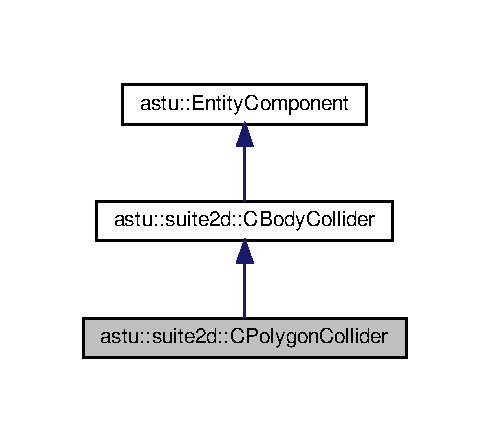
\includegraphics[width=235pt]{classastu_1_1suite2d_1_1CPolygonCollider__inherit__graph}
\end{center}
\end{figure}


Collaboration diagram for astu\+:\+:suite2d\+:\+:C\+Polygon\+Collider\+:\nopagebreak
\begin{figure}[H]
\begin{center}
\leavevmode
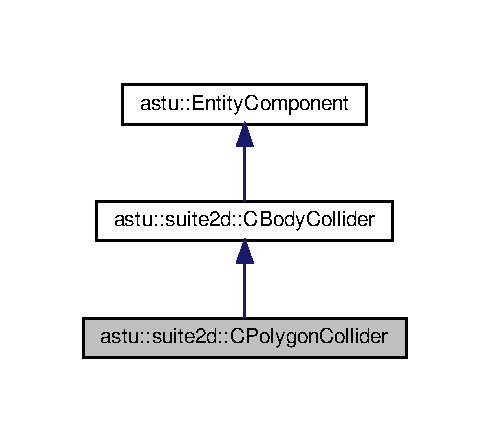
\includegraphics[width=235pt]{classastu_1_1suite2d_1_1CPolygonCollider__coll__graph}
\end{center}
\end{figure}
\subsection*{Public Member Functions}
\begin{DoxyCompactItemize}
\item 
\hyperlink{classastu_1_1suite2d_1_1CPolygonCollider_ab2ff37774a48bd159166ac89764aa384}{C\+Polygon\+Collider} ()
\item 
void \hyperlink{classastu_1_1suite2d_1_1CPolygonCollider_ac3f4b3c6885f72270ecde8ec8a8a4ed5}{Set\+Polygon} (std\+::shared\+\_\+ptr$<$ const \hyperlink{group__math__group_ga39ca0cd425ff5edd2a090d6997ce8c2a}{Polygon2f} $>$ poly)
\item 
virtual void \hyperlink{classastu_1_1suite2d_1_1CPolygonCollider_ac30165a676e92f89e1a840f858d9a050}{On\+Added\+To\+Entity} (\hyperlink{classastu_1_1Entity}{Entity} \&entity)
\end{DoxyCompactItemize}
\subsection*{Protected Attributes}
\begin{DoxyCompactItemize}
\item 
std\+::shared\+\_\+ptr$<$ const \hyperlink{group__math__group_ga39ca0cd425ff5edd2a090d6997ce8c2a}{Polygon2f} $>$ \hyperlink{classastu_1_1suite2d_1_1CPolygonCollider_a5fdae8e0614b5810fb2d1add8b7daf87}{polygon}
\end{DoxyCompactItemize}


\subsection{Detailed Description}
Polygonal collider. 

\subsection{Constructor \& Destructor Documentation}
\mbox{\Hypertarget{classastu_1_1suite2d_1_1CPolygonCollider_ab2ff37774a48bd159166ac89764aa384}\label{classastu_1_1suite2d_1_1CPolygonCollider_ab2ff37774a48bd159166ac89764aa384}} 
\index{astu\+::suite2d\+::\+C\+Polygon\+Collider@{astu\+::suite2d\+::\+C\+Polygon\+Collider}!C\+Polygon\+Collider@{C\+Polygon\+Collider}}
\index{C\+Polygon\+Collider@{C\+Polygon\+Collider}!astu\+::suite2d\+::\+C\+Polygon\+Collider@{astu\+::suite2d\+::\+C\+Polygon\+Collider}}
\subsubsection{\texorpdfstring{C\+Polygon\+Collider()}{CPolygonCollider()}}
{\footnotesize\ttfamily astu\+::suite2d\+::\+C\+Polygon\+Collider\+::\+C\+Polygon\+Collider (\begin{DoxyParamCaption}{ }\end{DoxyParamCaption})\hspace{0.3cm}{\ttfamily [inline]}}

Constructor. 

\subsection{Member Function Documentation}
\mbox{\Hypertarget{classastu_1_1suite2d_1_1CPolygonCollider_ac30165a676e92f89e1a840f858d9a050}\label{classastu_1_1suite2d_1_1CPolygonCollider_ac30165a676e92f89e1a840f858d9a050}} 
\index{astu\+::suite2d\+::\+C\+Polygon\+Collider@{astu\+::suite2d\+::\+C\+Polygon\+Collider}!On\+Added\+To\+Entity@{On\+Added\+To\+Entity}}
\index{On\+Added\+To\+Entity@{On\+Added\+To\+Entity}!astu\+::suite2d\+::\+C\+Polygon\+Collider@{astu\+::suite2d\+::\+C\+Polygon\+Collider}}
\subsubsection{\texorpdfstring{On\+Added\+To\+Entity()}{OnAddedToEntity()}}
{\footnotesize\ttfamily virtual void astu\+::suite2d\+::\+C\+Polygon\+Collider\+::\+On\+Added\+To\+Entity (\begin{DoxyParamCaption}\item[{\hyperlink{classastu_1_1Entity}{Entity} \&}]{entity }\end{DoxyParamCaption})\hspace{0.3cm}{\ttfamily [inline]}, {\ttfamily [virtual]}}

Called when added to an entity.

Most components do not need to override this method. Is is used occasionally to register additional interfaces a component implements. Registering implemented interfaces is necessary in order to make a component accessible via this interface and not just by the component type itself.


\begin{DoxyParams}{Parameters}
{\em entity} & the entity this component has been added to \\
\hline
\end{DoxyParams}


Reimplemented from \hyperlink{classastu_1_1EntityComponent_a8736f12dc9d2be7d2569408fc1040480}{astu\+::\+Entity\+Component}.

\mbox{\Hypertarget{classastu_1_1suite2d_1_1CPolygonCollider_ac3f4b3c6885f72270ecde8ec8a8a4ed5}\label{classastu_1_1suite2d_1_1CPolygonCollider_ac3f4b3c6885f72270ecde8ec8a8a4ed5}} 
\index{astu\+::suite2d\+::\+C\+Polygon\+Collider@{astu\+::suite2d\+::\+C\+Polygon\+Collider}!Set\+Polygon@{Set\+Polygon}}
\index{Set\+Polygon@{Set\+Polygon}!astu\+::suite2d\+::\+C\+Polygon\+Collider@{astu\+::suite2d\+::\+C\+Polygon\+Collider}}
\subsubsection{\texorpdfstring{Set\+Polygon()}{SetPolygon()}}
{\footnotesize\ttfamily void astu\+::suite2d\+::\+C\+Polygon\+Collider\+::\+Set\+Polygon (\begin{DoxyParamCaption}\item[{std\+::shared\+\_\+ptr$<$ const \hyperlink{group__math__group_ga39ca0cd425ff5edd2a090d6997ce8c2a}{Polygon2f} $>$}]{poly }\end{DoxyParamCaption})\hspace{0.3cm}{\ttfamily [inline]}}

Sets the polygon of this collider.


\begin{DoxyParams}{Parameters}
{\em poly} & the polygon \\
\hline
\end{DoxyParams}


\subsection{Member Data Documentation}
\mbox{\Hypertarget{classastu_1_1suite2d_1_1CPolygonCollider_a5fdae8e0614b5810fb2d1add8b7daf87}\label{classastu_1_1suite2d_1_1CPolygonCollider_a5fdae8e0614b5810fb2d1add8b7daf87}} 
\index{astu\+::suite2d\+::\+C\+Polygon\+Collider@{astu\+::suite2d\+::\+C\+Polygon\+Collider}!polygon@{polygon}}
\index{polygon@{polygon}!astu\+::suite2d\+::\+C\+Polygon\+Collider@{astu\+::suite2d\+::\+C\+Polygon\+Collider}}
\subsubsection{\texorpdfstring{polygon}{polygon}}
{\footnotesize\ttfamily std\+::shared\+\_\+ptr$<$const \hyperlink{group__math__group_ga39ca0cd425ff5edd2a090d6997ce8c2a}{Polygon2f}$>$ astu\+::suite2d\+::\+C\+Polygon\+Collider\+::polygon\hspace{0.3cm}{\ttfamily [protected]}}

The polygon defining the shape of this collider. 

The documentation for this class was generated from the following file\+:\begin{DoxyCompactItemize}
\item 
include/\+Suite2\+D/C\+Colliders.\+h\end{DoxyCompactItemize}

\hypertarget{classastu_1_1suite2d_1_1CPolygonColliderBuilder}{}\section{astu\+:\+:suite2d\+:\+:C\+Polygon\+Collider\+Builder Class Reference}
\label{classastu_1_1suite2d_1_1CPolygonColliderBuilder}\index{astu\+::suite2d\+::\+C\+Polygon\+Collider\+Builder@{astu\+::suite2d\+::\+C\+Polygon\+Collider\+Builder}}


{\ttfamily \#include $<$C\+Colliders.\+h$>$}



Inheritance diagram for astu\+:\+:suite2d\+:\+:C\+Polygon\+Collider\+Builder\+:\nopagebreak
\begin{figure}[H]
\begin{center}
\leavevmode
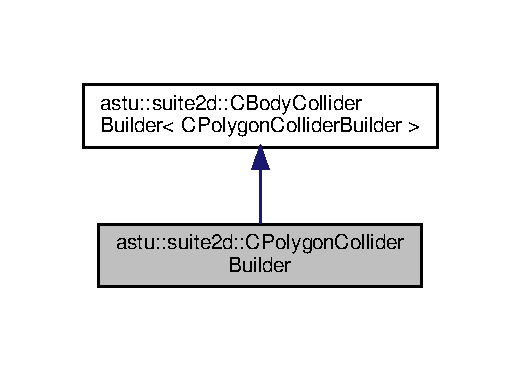
\includegraphics[width=250pt]{classastu_1_1suite2d_1_1CPolygonColliderBuilder__inherit__graph}
\end{center}
\end{figure}


Collaboration diagram for astu\+:\+:suite2d\+:\+:C\+Polygon\+Collider\+Builder\+:\nopagebreak
\begin{figure}[H]
\begin{center}
\leavevmode
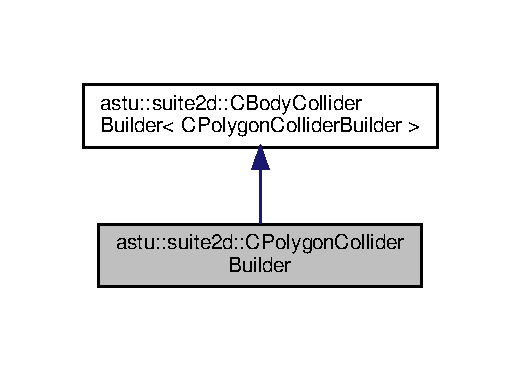
\includegraphics[width=250pt]{classastu_1_1suite2d_1_1CPolygonColliderBuilder__coll__graph}
\end{center}
\end{figure}
\subsection*{Public Member Functions}
\begin{DoxyCompactItemize}
\item 
\hyperlink{classastu_1_1suite2d_1_1CPolygonColliderBuilder_aea66d3118aedf7748ccb3bd6115f2961}{C\+Polygon\+Collider\+Builder} (std\+::shared\+\_\+ptr$<$ \hyperlink{classastu_1_1suite2d_1_1CPolygonColliderFactory}{C\+Polygon\+Collider\+Factory} $>$ collider\+Factory=nullptr)
\item 
\hyperlink{classastu_1_1suite2d_1_1CPolygonColliderBuilder}{C\+Polygon\+Collider\+Builder} \& \hyperlink{classastu_1_1suite2d_1_1CPolygonColliderBuilder_a5b4a20190025ac8a54e4c6da2ef55cf7}{Polygon} (std\+::shared\+\_\+ptr$<$ const \hyperlink{group__math__group_ga39ca0cd425ff5edd2a090d6997ce8c2a}{Polygon2f} $>$ poly)
\item 
\hyperlink{classastu_1_1suite2d_1_1CPolygonColliderBuilder}{C\+Polygon\+Collider\+Builder} \& \hyperlink{classastu_1_1suite2d_1_1CPolygonColliderBuilder_a11e3b9cace57e712bfae12de926458bb}{Polygon} (const std\+::vector$<$ \hyperlink{classastu_1_1Vector2}{Vector2f} $>$ \&vertices)
\item 
\hyperlink{classastu_1_1suite2d_1_1CPolygonColliderBuilder}{C\+Polygon\+Collider\+Builder} \& \hyperlink{classastu_1_1suite2d_1_1CPolygonColliderBuilder_a05b7196e63bc3466a31fefc6df121a58}{Make\+Rectangle} (float width, float height)
\item 
\hyperlink{classastu_1_1suite2d_1_1CPolygonColliderBuilder}{C\+Polygon\+Collider\+Builder} \& \hyperlink{classastu_1_1suite2d_1_1CPolygonColliderBuilder_ac8d3cf69f1fc687ab4aef32aa12383df}{Reset} ()
\item 
std\+::shared\+\_\+ptr$<$ \hyperlink{classastu_1_1suite2d_1_1CPolygonCollider}{C\+Polygon\+Collider} $>$ \hyperlink{classastu_1_1suite2d_1_1CPolygonColliderBuilder_a0ddc14822d47cf0fe115ed47d7c3095e}{Build} ()
\end{DoxyCompactItemize}
\subsection*{Additional Inherited Members}


\subsection{Detailed Description}
Builds \hyperlink{classastu_1_1suite2d_1_1CPolygonCollider}{C\+Polygon\+Collider} instances. 

\subsection{Constructor \& Destructor Documentation}
\mbox{\Hypertarget{classastu_1_1suite2d_1_1CPolygonColliderBuilder_aea66d3118aedf7748ccb3bd6115f2961}\label{classastu_1_1suite2d_1_1CPolygonColliderBuilder_aea66d3118aedf7748ccb3bd6115f2961}} 
\index{astu\+::suite2d\+::\+C\+Polygon\+Collider\+Builder@{astu\+::suite2d\+::\+C\+Polygon\+Collider\+Builder}!C\+Polygon\+Collider\+Builder@{C\+Polygon\+Collider\+Builder}}
\index{C\+Polygon\+Collider\+Builder@{C\+Polygon\+Collider\+Builder}!astu\+::suite2d\+::\+C\+Polygon\+Collider\+Builder@{astu\+::suite2d\+::\+C\+Polygon\+Collider\+Builder}}
\subsubsection{\texorpdfstring{C\+Polygon\+Collider\+Builder()}{CPolygonColliderBuilder()}}
{\footnotesize\ttfamily astu\+::suite2d\+::\+C\+Polygon\+Collider\+Builder\+::\+C\+Polygon\+Collider\+Builder (\begin{DoxyParamCaption}\item[{std\+::shared\+\_\+ptr$<$ \hyperlink{classastu_1_1suite2d_1_1CPolygonColliderFactory}{C\+Polygon\+Collider\+Factory} $>$}]{collider\+Factory = {\ttfamily nullptr} }\end{DoxyParamCaption})}

Constructor.

If the specified collider factory is null a service which implements the collider factory interface will be used.


\begin{DoxyParams}{Parameters}
{\em collider\+Factory} & the factory used to create new instances \\
\hline
\end{DoxyParams}


\subsection{Member Function Documentation}
\mbox{\Hypertarget{classastu_1_1suite2d_1_1CPolygonColliderBuilder_a0ddc14822d47cf0fe115ed47d7c3095e}\label{classastu_1_1suite2d_1_1CPolygonColliderBuilder_a0ddc14822d47cf0fe115ed47d7c3095e}} 
\index{astu\+::suite2d\+::\+C\+Polygon\+Collider\+Builder@{astu\+::suite2d\+::\+C\+Polygon\+Collider\+Builder}!Build@{Build}}
\index{Build@{Build}!astu\+::suite2d\+::\+C\+Polygon\+Collider\+Builder@{astu\+::suite2d\+::\+C\+Polygon\+Collider\+Builder}}
\subsubsection{\texorpdfstring{Build()}{Build()}}
{\footnotesize\ttfamily std\+::shared\+\_\+ptr$<$\hyperlink{classastu_1_1suite2d_1_1CPolygonCollider}{C\+Polygon\+Collider}$>$ astu\+::suite2d\+::\+C\+Polygon\+Collider\+Builder\+::\+Build (\begin{DoxyParamCaption}{ }\end{DoxyParamCaption})}

Builds a new polygon collider according to the current configuration.

\begin{DoxyReturn}{Returns}
the newly created polygon collider 
\end{DoxyReturn}
\mbox{\Hypertarget{classastu_1_1suite2d_1_1CPolygonColliderBuilder_a05b7196e63bc3466a31fefc6df121a58}\label{classastu_1_1suite2d_1_1CPolygonColliderBuilder_a05b7196e63bc3466a31fefc6df121a58}} 
\index{astu\+::suite2d\+::\+C\+Polygon\+Collider\+Builder@{astu\+::suite2d\+::\+C\+Polygon\+Collider\+Builder}!Make\+Rectangle@{Make\+Rectangle}}
\index{Make\+Rectangle@{Make\+Rectangle}!astu\+::suite2d\+::\+C\+Polygon\+Collider\+Builder@{astu\+::suite2d\+::\+C\+Polygon\+Collider\+Builder}}
\subsubsection{\texorpdfstring{Make\+Rectangle()}{MakeRectangle()}}
{\footnotesize\ttfamily \hyperlink{classastu_1_1suite2d_1_1CPolygonColliderBuilder}{C\+Polygon\+Collider\+Builder}\& astu\+::suite2d\+::\+C\+Polygon\+Collider\+Builder\+::\+Make\+Rectangle (\begin{DoxyParamCaption}\item[{float}]{width,  }\item[{float}]{height }\end{DoxyParamCaption})}

Set the polygon to an axis aligned rectangle.


\begin{DoxyParams}{Parameters}
{\em width} & the width of the rectangle \\
\hline
{\em height} & the height of the rectangle \\
\hline
\end{DoxyParams}
\begin{DoxyReturn}{Returns}
reference to this builder for method chaining 
\end{DoxyReturn}
\mbox{\Hypertarget{classastu_1_1suite2d_1_1CPolygonColliderBuilder_a5b4a20190025ac8a54e4c6da2ef55cf7}\label{classastu_1_1suite2d_1_1CPolygonColliderBuilder_a5b4a20190025ac8a54e4c6da2ef55cf7}} 
\index{astu\+::suite2d\+::\+C\+Polygon\+Collider\+Builder@{astu\+::suite2d\+::\+C\+Polygon\+Collider\+Builder}!Polygon@{Polygon}}
\index{Polygon@{Polygon}!astu\+::suite2d\+::\+C\+Polygon\+Collider\+Builder@{astu\+::suite2d\+::\+C\+Polygon\+Collider\+Builder}}
\subsubsection{\texorpdfstring{Polygon()}{Polygon()}\hspace{0.1cm}{\footnotesize\ttfamily [1/2]}}
{\footnotesize\ttfamily \hyperlink{classastu_1_1suite2d_1_1CPolygonColliderBuilder}{C\+Polygon\+Collider\+Builder}\& astu\+::suite2d\+::\+C\+Polygon\+Collider\+Builder\+::\+Polygon (\begin{DoxyParamCaption}\item[{std\+::shared\+\_\+ptr$<$ const \hyperlink{group__math__group_ga39ca0cd425ff5edd2a090d6997ce8c2a}{Polygon2f} $>$}]{poly }\end{DoxyParamCaption})\hspace{0.3cm}{\ttfamily [inline]}}

Sets the polygon of the polygon collider to build.


\begin{DoxyParams}{Parameters}
{\em poly} & the polygon of the collider \\
\hline
\end{DoxyParams}
\begin{DoxyReturn}{Returns}
reference to this builder for method chaining 
\end{DoxyReturn}
\mbox{\Hypertarget{classastu_1_1suite2d_1_1CPolygonColliderBuilder_a11e3b9cace57e712bfae12de926458bb}\label{classastu_1_1suite2d_1_1CPolygonColliderBuilder_a11e3b9cace57e712bfae12de926458bb}} 
\index{astu\+::suite2d\+::\+C\+Polygon\+Collider\+Builder@{astu\+::suite2d\+::\+C\+Polygon\+Collider\+Builder}!Polygon@{Polygon}}
\index{Polygon@{Polygon}!astu\+::suite2d\+::\+C\+Polygon\+Collider\+Builder@{astu\+::suite2d\+::\+C\+Polygon\+Collider\+Builder}}
\subsubsection{\texorpdfstring{Polygon()}{Polygon()}\hspace{0.1cm}{\footnotesize\ttfamily [2/2]}}
{\footnotesize\ttfamily \hyperlink{classastu_1_1suite2d_1_1CPolygonColliderBuilder}{C\+Polygon\+Collider\+Builder}\& astu\+::suite2d\+::\+C\+Polygon\+Collider\+Builder\+::\+Polygon (\begin{DoxyParamCaption}\item[{const std\+::vector$<$ \hyperlink{classastu_1_1Vector2}{Vector2f} $>$ \&}]{vertices }\end{DoxyParamCaption})\hspace{0.3cm}{\ttfamily [inline]}}

Sets the polygon of the polygon collider to build.


\begin{DoxyParams}{Parameters}
{\em vertices} & the vertices that make up the polygon \\
\hline
\end{DoxyParams}
\begin{DoxyReturn}{Returns}
reference to this builder for method chaining 
\end{DoxyReturn}
\mbox{\Hypertarget{classastu_1_1suite2d_1_1CPolygonColliderBuilder_ac8d3cf69f1fc687ab4aef32aa12383df}\label{classastu_1_1suite2d_1_1CPolygonColliderBuilder_ac8d3cf69f1fc687ab4aef32aa12383df}} 
\index{astu\+::suite2d\+::\+C\+Polygon\+Collider\+Builder@{astu\+::suite2d\+::\+C\+Polygon\+Collider\+Builder}!Reset@{Reset}}
\index{Reset@{Reset}!astu\+::suite2d\+::\+C\+Polygon\+Collider\+Builder@{astu\+::suite2d\+::\+C\+Polygon\+Collider\+Builder}}
\subsubsection{\texorpdfstring{Reset()}{Reset()}}
{\footnotesize\ttfamily \hyperlink{classastu_1_1suite2d_1_1CPolygonColliderBuilder}{C\+Polygon\+Collider\+Builder}\& astu\+::suite2d\+::\+C\+Polygon\+Collider\+Builder\+::\+Reset (\begin{DoxyParamCaption}{ }\end{DoxyParamCaption})\hspace{0.3cm}{\ttfamily [inline]}}

Resets this builder to its initial configuration.

\begin{DoxyReturn}{Returns}
reference to this builder for method chaining 
\end{DoxyReturn}


The documentation for this class was generated from the following file\+:\begin{DoxyCompactItemize}
\item 
include/\+Suite2\+D/C\+Colliders.\+h\end{DoxyCompactItemize}

\hypertarget{classastu_1_1suite2d_1_1CPolygonColliderFactory}{}\section{astu\+:\+:suite2d\+:\+:C\+Polygon\+Collider\+Factory Class Reference}
\label{classastu_1_1suite2d_1_1CPolygonColliderFactory}\index{astu\+::suite2d\+::\+C\+Polygon\+Collider\+Factory@{astu\+::suite2d\+::\+C\+Polygon\+Collider\+Factory}}


{\ttfamily \#include $<$C\+Colliders.\+h$>$}

\subsection*{Public Member Functions}
\begin{DoxyCompactItemize}
\item 
virtual \hyperlink{classastu_1_1suite2d_1_1CPolygonColliderFactory_ad8db117ac2def0fd39b77c718cc875bc}{$\sim$\+C\+Polygon\+Collider\+Factory} ()
\item 
virtual std\+::shared\+\_\+ptr$<$ \hyperlink{classastu_1_1suite2d_1_1CPolygonCollider}{C\+Polygon\+Collider} $>$ \hyperlink{classastu_1_1suite2d_1_1CPolygonColliderFactory_a29ecb824aa282ce5c6d64111d9bfd65f}{Create\+Polygon\+Collider} ()=0
\end{DoxyCompactItemize}


\subsection{Detailed Description}
Abstract factory for for \hyperlink{classastu_1_1suite2d_1_1CPolygonCollider}{C\+Polygon\+Collider} components. 

\subsection{Constructor \& Destructor Documentation}
\mbox{\Hypertarget{classastu_1_1suite2d_1_1CPolygonColliderFactory_ad8db117ac2def0fd39b77c718cc875bc}\label{classastu_1_1suite2d_1_1CPolygonColliderFactory_ad8db117ac2def0fd39b77c718cc875bc}} 
\index{astu\+::suite2d\+::\+C\+Polygon\+Collider\+Factory@{astu\+::suite2d\+::\+C\+Polygon\+Collider\+Factory}!````~C\+Polygon\+Collider\+Factory@{$\sim$\+C\+Polygon\+Collider\+Factory}}
\index{````~C\+Polygon\+Collider\+Factory@{$\sim$\+C\+Polygon\+Collider\+Factory}!astu\+::suite2d\+::\+C\+Polygon\+Collider\+Factory@{astu\+::suite2d\+::\+C\+Polygon\+Collider\+Factory}}
\subsubsection{\texorpdfstring{$\sim$\+C\+Polygon\+Collider\+Factory()}{~CPolygonColliderFactory()}}
{\footnotesize\ttfamily virtual astu\+::suite2d\+::\+C\+Polygon\+Collider\+Factory\+::$\sim$\+C\+Polygon\+Collider\+Factory (\begin{DoxyParamCaption}{ }\end{DoxyParamCaption})\hspace{0.3cm}{\ttfamily [inline]}, {\ttfamily [virtual]}}

Virtual destructor. 

\subsection{Member Function Documentation}
\mbox{\Hypertarget{classastu_1_1suite2d_1_1CPolygonColliderFactory_a29ecb824aa282ce5c6d64111d9bfd65f}\label{classastu_1_1suite2d_1_1CPolygonColliderFactory_a29ecb824aa282ce5c6d64111d9bfd65f}} 
\index{astu\+::suite2d\+::\+C\+Polygon\+Collider\+Factory@{astu\+::suite2d\+::\+C\+Polygon\+Collider\+Factory}!Create\+Polygon\+Collider@{Create\+Polygon\+Collider}}
\index{Create\+Polygon\+Collider@{Create\+Polygon\+Collider}!astu\+::suite2d\+::\+C\+Polygon\+Collider\+Factory@{astu\+::suite2d\+::\+C\+Polygon\+Collider\+Factory}}
\subsubsection{\texorpdfstring{Create\+Polygon\+Collider()}{CreatePolygonCollider()}}
{\footnotesize\ttfamily virtual std\+::shared\+\_\+ptr$<$\hyperlink{classastu_1_1suite2d_1_1CPolygonCollider}{C\+Polygon\+Collider}$>$ astu\+::suite2d\+::\+C\+Polygon\+Collider\+Factory\+::\+Create\+Polygon\+Collider (\begin{DoxyParamCaption}{ }\end{DoxyParamCaption})\hspace{0.3cm}{\ttfamily [pure virtual]}}

Creates a new \hyperlink{classastu_1_1suite2d_1_1CCircleCollider}{C\+Circle\+Collider} instance. 

The documentation for this class was generated from the following file\+:\begin{DoxyCompactItemize}
\item 
include/\+Suite2\+D/C\+Colliders.\+h\end{DoxyCompactItemize}

\hypertarget{classastu_1_1suite2d_1_1CPose}{}\section{astu\+:\+:suite2d\+:\+:C\+Pose Class Reference}
\label{classastu_1_1suite2d_1_1CPose}\index{astu\+::suite2d\+::\+C\+Pose@{astu\+::suite2d\+::\+C\+Pose}}


{\ttfamily \#include $<$C\+Pose.\+h$>$}



Inheritance diagram for astu\+:\+:suite2d\+:\+:C\+Pose\+:\nopagebreak
\begin{figure}[H]
\begin{center}
\leavevmode
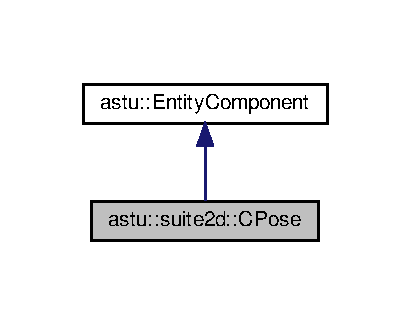
\includegraphics[width=197pt]{classastu_1_1suite2d_1_1CPose__inherit__graph}
\end{center}
\end{figure}


Collaboration diagram for astu\+:\+:suite2d\+:\+:C\+Pose\+:\nopagebreak
\begin{figure}[H]
\begin{center}
\leavevmode
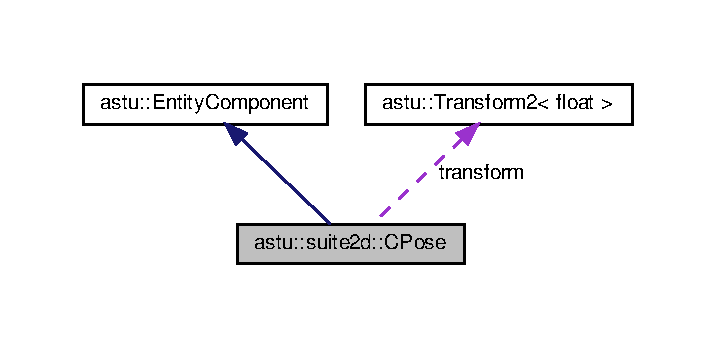
\includegraphics[width=344pt]{classastu_1_1suite2d_1_1CPose__coll__graph}
\end{center}
\end{figure}
\subsection*{Public Member Functions}
\begin{DoxyCompactItemize}
\item 
\hyperlink{classastu_1_1suite2d_1_1CPose_ae43f407c724a21294a886ae9fc0a4d60}{C\+Pose} ()
\item 
\hyperlink{classastu_1_1suite2d_1_1CPose_a84da6beb4c3f58a90eee567a649cabf4}{C\+Pose} (float x, float y, float phi=0)
\item 
virtual std\+::shared\+\_\+ptr$<$ \hyperlink{classastu_1_1EntityComponent}{Entity\+Component} $>$ \hyperlink{classastu_1_1suite2d_1_1CPose_a90d4fb820221ddabf9c95d5a10796359}{Clone} () override
\end{DoxyCompactItemize}
\subsection*{Public Attributes}
\begin{DoxyCompactItemize}
\item 
\hyperlink{classastu_1_1Transform2}{astu\+::\+Transform2}$<$ float $>$ \hyperlink{classastu_1_1suite2d_1_1CPose_af9c1225512bc213fdaff45008416654c}{transform}
\end{DoxyCompactItemize}


\subsection{Detailed Description}
An entity component which describes the position and orientation in two-\/dimensional world space. 

\subsection{Constructor \& Destructor Documentation}
\mbox{\Hypertarget{classastu_1_1suite2d_1_1CPose_ae43f407c724a21294a886ae9fc0a4d60}\label{classastu_1_1suite2d_1_1CPose_ae43f407c724a21294a886ae9fc0a4d60}} 
\index{astu\+::suite2d\+::\+C\+Pose@{astu\+::suite2d\+::\+C\+Pose}!C\+Pose@{C\+Pose}}
\index{C\+Pose@{C\+Pose}!astu\+::suite2d\+::\+C\+Pose@{astu\+::suite2d\+::\+C\+Pose}}
\subsubsection{\texorpdfstring{C\+Pose()}{CPose()}\hspace{0.1cm}{\footnotesize\ttfamily [1/2]}}
{\footnotesize\ttfamily astu\+::suite2d\+::\+C\+Pose\+::\+C\+Pose (\begin{DoxyParamCaption}{ }\end{DoxyParamCaption})\hspace{0.3cm}{\ttfamily [inline]}}

Constructor. \mbox{\Hypertarget{classastu_1_1suite2d_1_1CPose_a84da6beb4c3f58a90eee567a649cabf4}\label{classastu_1_1suite2d_1_1CPose_a84da6beb4c3f58a90eee567a649cabf4}} 
\index{astu\+::suite2d\+::\+C\+Pose@{astu\+::suite2d\+::\+C\+Pose}!C\+Pose@{C\+Pose}}
\index{C\+Pose@{C\+Pose}!astu\+::suite2d\+::\+C\+Pose@{astu\+::suite2d\+::\+C\+Pose}}
\subsubsection{\texorpdfstring{C\+Pose()}{CPose()}\hspace{0.1cm}{\footnotesize\ttfamily [2/2]}}
{\footnotesize\ttfamily astu\+::suite2d\+::\+C\+Pose\+::\+C\+Pose (\begin{DoxyParamCaption}\item[{float}]{x,  }\item[{float}]{y,  }\item[{float}]{phi = {\ttfamily 0} }\end{DoxyParamCaption})\hspace{0.3cm}{\ttfamily [inline]}}

Constructor.


\begin{DoxyParams}{Parameters}
{\em x} & the x-\/coordinate of the initial translation \\
\hline
{\em y} & the y-\/coordinate of the initial translation \\
\hline
{\em phi} & the angle of the initial rotation in radians \\
\hline
\end{DoxyParams}


\subsection{Member Function Documentation}
\mbox{\Hypertarget{classastu_1_1suite2d_1_1CPose_a90d4fb820221ddabf9c95d5a10796359}\label{classastu_1_1suite2d_1_1CPose_a90d4fb820221ddabf9c95d5a10796359}} 
\index{astu\+::suite2d\+::\+C\+Pose@{astu\+::suite2d\+::\+C\+Pose}!Clone@{Clone}}
\index{Clone@{Clone}!astu\+::suite2d\+::\+C\+Pose@{astu\+::suite2d\+::\+C\+Pose}}
\subsubsection{\texorpdfstring{Clone()}{Clone()}}
{\footnotesize\ttfamily virtual std\+::shared\+\_\+ptr$<$\hyperlink{classastu_1_1EntityComponent}{Entity\+Component}$>$ astu\+::suite2d\+::\+C\+Pose\+::\+Clone (\begin{DoxyParamCaption}{ }\end{DoxyParamCaption})\hspace{0.3cm}{\ttfamily [inline]}, {\ttfamily [override]}, {\ttfamily [virtual]}}

Creates a copy of this entity component.

\begin{DoxyReturn}{Returns}
a copy of this componend 
\end{DoxyReturn}


Implements \hyperlink{classastu_1_1EntityComponent_afeddb5a899d831255a9a4f07269f3b2d}{astu\+::\+Entity\+Component}.



\subsection{Member Data Documentation}
\mbox{\Hypertarget{classastu_1_1suite2d_1_1CPose_af9c1225512bc213fdaff45008416654c}\label{classastu_1_1suite2d_1_1CPose_af9c1225512bc213fdaff45008416654c}} 
\index{astu\+::suite2d\+::\+C\+Pose@{astu\+::suite2d\+::\+C\+Pose}!transform@{transform}}
\index{transform@{transform}!astu\+::suite2d\+::\+C\+Pose@{astu\+::suite2d\+::\+C\+Pose}}
\subsubsection{\texorpdfstring{transform}{transform}}
{\footnotesize\ttfamily \hyperlink{classastu_1_1Transform2}{astu\+::\+Transform2}$<$float$>$ astu\+::suite2d\+::\+C\+Pose\+::transform}

The transformation. 

The documentation for this class was generated from the following file\+:\begin{DoxyCompactItemize}
\item 
include/\+Suite2\+D/C\+Pose.\+h\end{DoxyCompactItemize}

\hypertarget{classastu_1_1suite2d_1_1CScene}{}\section{astu\+:\+:suite2d\+:\+:C\+Scene Class Reference}
\label{classastu_1_1suite2d_1_1CScene}\index{astu\+::suite2d\+::\+C\+Scene@{astu\+::suite2d\+::\+C\+Scene}}


{\ttfamily \#include $<$C\+Scene.\+h$>$}



Inheritance diagram for astu\+:\+:suite2d\+:\+:C\+Scene\+:\nopagebreak
\begin{figure}[H]
\begin{center}
\leavevmode
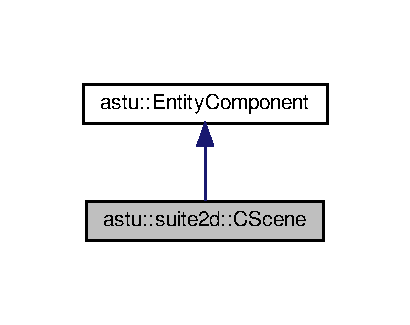
\includegraphics[width=197pt]{classastu_1_1suite2d_1_1CScene__inherit__graph}
\end{center}
\end{figure}


Collaboration diagram for astu\+:\+:suite2d\+:\+:C\+Scene\+:\nopagebreak
\begin{figure}[H]
\begin{center}
\leavevmode
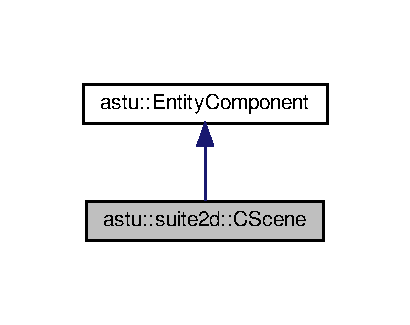
\includegraphics[width=197pt]{classastu_1_1suite2d_1_1CScene__coll__graph}
\end{center}
\end{figure}
\subsection*{Public Member Functions}
\begin{DoxyCompactItemize}
\item 
\hyperlink{classastu_1_1suite2d_1_1CScene_afdee9d9f1214ccfd36b44f68d5e351fa}{C\+Scene} (std\+::shared\+\_\+ptr$<$ \hyperlink{classastu_1_1suite2d_1_1Spatial}{Spatial} $>$ \hyperlink{classastu_1_1suite2d_1_1CScene_af8b497f2d0dac0c1bb4d7d3038280189}{spatial})
\item 
virtual std\+::shared\+\_\+ptr$<$ \hyperlink{classastu_1_1EntityComponent}{astu\+::\+Entity\+Component} $>$ \hyperlink{classastu_1_1suite2d_1_1CScene_ae8dad316175ec4bbfbdb7fff3c736cd3}{Clone} () override
\end{DoxyCompactItemize}
\subsection*{Public Attributes}
\begin{DoxyCompactItemize}
\item 
std\+::shared\+\_\+ptr$<$ \hyperlink{classastu_1_1suite2d_1_1Spatial}{Spatial} $>$ \hyperlink{classastu_1_1suite2d_1_1CScene_af8b497f2d0dac0c1bb4d7d3038280189}{spatial}
\end{DoxyCompactItemize}


\subsection{Detailed Description}
A component containing a spacial 2D scene graph element.

This type of component is typically used for visual representation of entities in two-\/dimensional worlds. 

\subsection{Constructor \& Destructor Documentation}
\mbox{\Hypertarget{classastu_1_1suite2d_1_1CScene_afdee9d9f1214ccfd36b44f68d5e351fa}\label{classastu_1_1suite2d_1_1CScene_afdee9d9f1214ccfd36b44f68d5e351fa}} 
\index{astu\+::suite2d\+::\+C\+Scene@{astu\+::suite2d\+::\+C\+Scene}!C\+Scene@{C\+Scene}}
\index{C\+Scene@{C\+Scene}!astu\+::suite2d\+::\+C\+Scene@{astu\+::suite2d\+::\+C\+Scene}}
\subsubsection{\texorpdfstring{C\+Scene()}{CScene()}}
{\footnotesize\ttfamily astu\+::suite2d\+::\+C\+Scene\+::\+C\+Scene (\begin{DoxyParamCaption}\item[{std\+::shared\+\_\+ptr$<$ \hyperlink{classastu_1_1suite2d_1_1Spatial}{Spatial} $>$}]{spatial }\end{DoxyParamCaption})\hspace{0.3cm}{\ttfamily [inline]}}

Constructor.


\begin{DoxyParams}{Parameters}
{\em spatial} & the scene node branch representing the entity \\
\hline
\end{DoxyParams}


\subsection{Member Function Documentation}
\mbox{\Hypertarget{classastu_1_1suite2d_1_1CScene_ae8dad316175ec4bbfbdb7fff3c736cd3}\label{classastu_1_1suite2d_1_1CScene_ae8dad316175ec4bbfbdb7fff3c736cd3}} 
\index{astu\+::suite2d\+::\+C\+Scene@{astu\+::suite2d\+::\+C\+Scene}!Clone@{Clone}}
\index{Clone@{Clone}!astu\+::suite2d\+::\+C\+Scene@{astu\+::suite2d\+::\+C\+Scene}}
\subsubsection{\texorpdfstring{Clone()}{Clone()}}
{\footnotesize\ttfamily virtual std\+::shared\+\_\+ptr$<$\hyperlink{classastu_1_1EntityComponent}{astu\+::\+Entity\+Component}$>$ astu\+::suite2d\+::\+C\+Scene\+::\+Clone (\begin{DoxyParamCaption}{ }\end{DoxyParamCaption})\hspace{0.3cm}{\ttfamily [inline]}, {\ttfamily [override]}, {\ttfamily [virtual]}}

Creates a copy of this entity component.

\begin{DoxyReturn}{Returns}
a copy of this componend 
\end{DoxyReturn}


Implements \hyperlink{classastu_1_1EntityComponent_afeddb5a899d831255a9a4f07269f3b2d}{astu\+::\+Entity\+Component}.



\subsection{Member Data Documentation}
\mbox{\Hypertarget{classastu_1_1suite2d_1_1CScene_af8b497f2d0dac0c1bb4d7d3038280189}\label{classastu_1_1suite2d_1_1CScene_af8b497f2d0dac0c1bb4d7d3038280189}} 
\index{astu\+::suite2d\+::\+C\+Scene@{astu\+::suite2d\+::\+C\+Scene}!spatial@{spatial}}
\index{spatial@{spatial}!astu\+::suite2d\+::\+C\+Scene@{astu\+::suite2d\+::\+C\+Scene}}
\subsubsection{\texorpdfstring{spatial}{spatial}}
{\footnotesize\ttfamily std\+::shared\+\_\+ptr$<$\hyperlink{classastu_1_1suite2d_1_1Spatial}{Spatial}$>$ astu\+::suite2d\+::\+C\+Scene\+::spatial}

Branch of the scene graph. 

The documentation for this class was generated from the following file\+:\begin{DoxyCompactItemize}
\item 
include/\+Suite2\+D/C\+Scene.\+h\end{DoxyCompactItemize}

\hypertarget{classastu_1_1DelegateTask}{}\section{astu\+:\+:Delegate\+Task Class Reference}
\label{classastu_1_1DelegateTask}\index{astu\+::\+Delegate\+Task@{astu\+::\+Delegate\+Task}}


{\ttfamily \#include $<$Tasks.\+h$>$}



Inheritance diagram for astu\+:\+:Delegate\+Task\+:\nopagebreak
\begin{figure}[H]
\begin{center}
\leavevmode
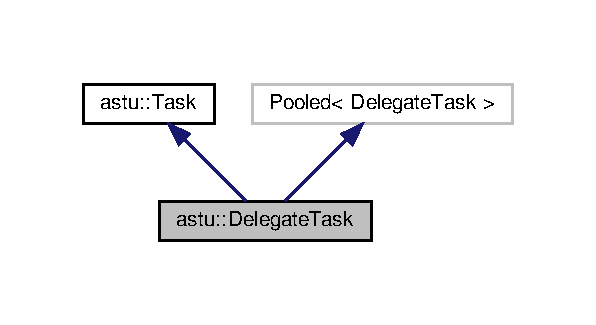
\includegraphics[width=286pt]{classastu_1_1DelegateTask__inherit__graph}
\end{center}
\end{figure}


Collaboration diagram for astu\+:\+:Delegate\+Task\+:\nopagebreak
\begin{figure}[H]
\begin{center}
\leavevmode
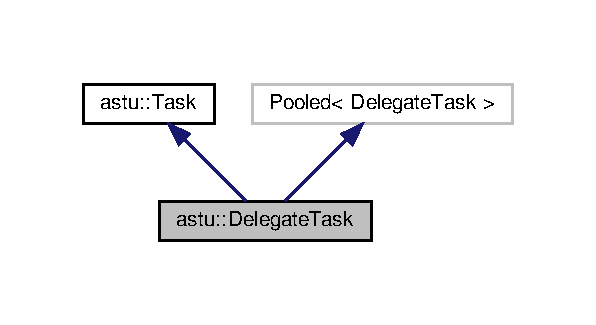
\includegraphics[width=286pt]{classastu_1_1DelegateTask__coll__graph}
\end{center}
\end{figure}
\subsection*{Public Types}
\begin{DoxyCompactItemize}
\item 
using \hyperlink{classastu_1_1DelegateTask_a74c7859178eb0889e884209d1604de4d}{Delegate} = std\+::function$<$ void(void)$>$
\end{DoxyCompactItemize}
\subsection*{Public Member Functions}
\begin{DoxyCompactItemize}
\item 
virtual \hyperlink{classastu_1_1DelegateTask_a948c5a93de18e5c9b6eafd247cdc849b}{$\sim$\+Delegate\+Task} ()
\item 
\mbox{\Hypertarget{classastu_1_1DelegateTask_a28429114340e8b692f8cc32ef65a8199}\label{classastu_1_1DelegateTask_a28429114340e8b692f8cc32ef65a8199}} 
{\bfseries Delegate\+Task} (const \hyperlink{classastu_1_1DelegateTask}{Delegate\+Task} \&)=delete
\item 
\mbox{\Hypertarget{classastu_1_1DelegateTask_ae0b4c2af0b5fd25270cc0e35784dc4ab}\label{classastu_1_1DelegateTask_ae0b4c2af0b5fd25270cc0e35784dc4ab}} 
\hyperlink{classastu_1_1DelegateTask}{Delegate\+Task} \& {\bfseries operator=} (const \hyperlink{classastu_1_1DelegateTask}{Delegate\+Task} \&)=delete
\item 
virtual void \hyperlink{classastu_1_1DelegateTask_a48755ab30194963c37e22ed118423704}{Update} (double dt) override
\item 
virtual void \hyperlink{classastu_1_1DelegateTask_a8bc7364937a4af2173e066174733e1d1}{Reset} () override
\end{DoxyCompactItemize}
\subsection*{Static Public Member Functions}
\begin{DoxyCompactItemize}
\item 
static std\+::unique\+\_\+ptr$<$ \hyperlink{classastu_1_1DelegateTask}{Delegate\+Task} $>$ \hyperlink{classastu_1_1DelegateTask_a3d27b0336f3f0ff70acef517312d9d37}{Create} (\hyperlink{classastu_1_1DelegateTask_a74c7859178eb0889e884209d1604de4d}{Delegate} delegate, double \hyperlink{classastu_1_1DelegateTask_a448096d7fea7f9a18490fbaa05616995}{delay}=1)
\end{DoxyCompactItemize}
\subsection*{Public Attributes}
\begin{DoxyCompactItemize}
\item 
double \hyperlink{classastu_1_1DelegateTask_a448096d7fea7f9a18490fbaa05616995}{delay}
\item 
double \hyperlink{classastu_1_1DelegateTask_ae192279cf06935c58ad19c28ac674e18}{elapsed\+Time}
\item 
\hyperlink{classastu_1_1DelegateTask_a74c7859178eb0889e884209d1604de4d}{Delegate} \hyperlink{classastu_1_1DelegateTask_a9dc938c77515b4be4501df66f8cb260c}{delegate\+Func}
\end{DoxyCompactItemize}
\subsection*{Additional Inherited Members}


\subsection{Detailed Description}
Calls a delegate after a specific amount of time. 

\subsection{Member Typedef Documentation}
\mbox{\Hypertarget{classastu_1_1DelegateTask_a74c7859178eb0889e884209d1604de4d}\label{classastu_1_1DelegateTask_a74c7859178eb0889e884209d1604de4d}} 
\index{astu\+::\+Delegate\+Task@{astu\+::\+Delegate\+Task}!Delegate@{Delegate}}
\index{Delegate@{Delegate}!astu\+::\+Delegate\+Task@{astu\+::\+Delegate\+Task}}
\subsubsection{\texorpdfstring{Delegate}{Delegate}}
{\footnotesize\ttfamily using \hyperlink{classastu_1_1DelegateTask_a74c7859178eb0889e884209d1604de4d}{astu\+::\+Delegate\+Task\+::\+Delegate} =  std\+::function$<$void (void)$>$}

Type alias for delegate functions. 

\subsection{Constructor \& Destructor Documentation}
\mbox{\Hypertarget{classastu_1_1DelegateTask_a948c5a93de18e5c9b6eafd247cdc849b}\label{classastu_1_1DelegateTask_a948c5a93de18e5c9b6eafd247cdc849b}} 
\index{astu\+::\+Delegate\+Task@{astu\+::\+Delegate\+Task}!````~Delegate\+Task@{$\sim$\+Delegate\+Task}}
\index{````~Delegate\+Task@{$\sim$\+Delegate\+Task}!astu\+::\+Delegate\+Task@{astu\+::\+Delegate\+Task}}
\subsubsection{\texorpdfstring{$\sim$\+Delegate\+Task()}{~DelegateTask()}}
{\footnotesize\ttfamily virtual astu\+::\+Delegate\+Task\+::$\sim$\+Delegate\+Task (\begin{DoxyParamCaption}{ }\end{DoxyParamCaption})\hspace{0.3cm}{\ttfamily [virtual]}}

Virtual destructor. 

\subsection{Member Function Documentation}
\mbox{\Hypertarget{classastu_1_1DelegateTask_a3d27b0336f3f0ff70acef517312d9d37}\label{classastu_1_1DelegateTask_a3d27b0336f3f0ff70acef517312d9d37}} 
\index{astu\+::\+Delegate\+Task@{astu\+::\+Delegate\+Task}!Create@{Create}}
\index{Create@{Create}!astu\+::\+Delegate\+Task@{astu\+::\+Delegate\+Task}}
\subsubsection{\texorpdfstring{Create()}{Create()}}
{\footnotesize\ttfamily static std\+::unique\+\_\+ptr$<$\hyperlink{classastu_1_1DelegateTask}{Delegate\+Task}$>$ astu\+::\+Delegate\+Task\+::\+Create (\begin{DoxyParamCaption}\item[{\hyperlink{classastu_1_1DelegateTask_a74c7859178eb0889e884209d1604de4d}{Delegate}}]{delegate,  }\item[{double}]{delay = {\ttfamily 1} }\end{DoxyParamCaption})\hspace{0.3cm}{\ttfamily [static]}}

Returns a new delegate instnace.


\begin{DoxyParams}{Parameters}
{\em delegate} & the delegate to call \\
\hline
{\em delay} & the time to wait in seconds \\
\hline
\end{DoxyParams}
\mbox{\Hypertarget{classastu_1_1DelegateTask_a8bc7364937a4af2173e066174733e1d1}\label{classastu_1_1DelegateTask_a8bc7364937a4af2173e066174733e1d1}} 
\index{astu\+::\+Delegate\+Task@{astu\+::\+Delegate\+Task}!Reset@{Reset}}
\index{Reset@{Reset}!astu\+::\+Delegate\+Task@{astu\+::\+Delegate\+Task}}
\subsubsection{\texorpdfstring{Reset()}{Reset()}}
{\footnotesize\ttfamily virtual void astu\+::\+Delegate\+Task\+::\+Reset (\begin{DoxyParamCaption}{ }\end{DoxyParamCaption})\hspace{0.3cm}{\ttfamily [override]}, {\ttfamily [virtual]}}

Resets this task to its initial condition. 

Reimplemented from \hyperlink{classastu_1_1Task_af68025df1de6ad31882f0ccee5ccb100}{astu\+::\+Task}.

\mbox{\Hypertarget{classastu_1_1DelegateTask_a48755ab30194963c37e22ed118423704}\label{classastu_1_1DelegateTask_a48755ab30194963c37e22ed118423704}} 
\index{astu\+::\+Delegate\+Task@{astu\+::\+Delegate\+Task}!Update@{Update}}
\index{Update@{Update}!astu\+::\+Delegate\+Task@{astu\+::\+Delegate\+Task}}
\subsubsection{\texorpdfstring{Update()}{Update()}}
{\footnotesize\ttfamily virtual void astu\+::\+Delegate\+Task\+::\+Update (\begin{DoxyParamCaption}\item[{double}]{dt }\end{DoxyParamCaption})\hspace{0.3cm}{\ttfamily [override]}, {\ttfamily [virtual]}}

Updates this task.


\begin{DoxyParams}{Parameters}
{\em dt} & the elapsed time since tha last update in seconds \\
\hline
\end{DoxyParams}


Implements \hyperlink{classastu_1_1Task_a2bcec3cc42b46cfcb03422e029577c0a}{astu\+::\+Task}.



\subsection{Member Data Documentation}
\mbox{\Hypertarget{classastu_1_1DelegateTask_a448096d7fea7f9a18490fbaa05616995}\label{classastu_1_1DelegateTask_a448096d7fea7f9a18490fbaa05616995}} 
\index{astu\+::\+Delegate\+Task@{astu\+::\+Delegate\+Task}!delay@{delay}}
\index{delay@{delay}!astu\+::\+Delegate\+Task@{astu\+::\+Delegate\+Task}}
\subsubsection{\texorpdfstring{delay}{delay}}
{\footnotesize\ttfamily double astu\+::\+Delegate\+Task\+::delay}

The duration to wait before to call the delegate. \mbox{\Hypertarget{classastu_1_1DelegateTask_a9dc938c77515b4be4501df66f8cb260c}\label{classastu_1_1DelegateTask_a9dc938c77515b4be4501df66f8cb260c}} 
\index{astu\+::\+Delegate\+Task@{astu\+::\+Delegate\+Task}!delegate\+Func@{delegate\+Func}}
\index{delegate\+Func@{delegate\+Func}!astu\+::\+Delegate\+Task@{astu\+::\+Delegate\+Task}}
\subsubsection{\texorpdfstring{delegate\+Func}{delegateFunc}}
{\footnotesize\ttfamily \hyperlink{classastu_1_1DelegateTask_a74c7859178eb0889e884209d1604de4d}{Delegate} astu\+::\+Delegate\+Task\+::delegate\+Func}

The delegate function to be called. \mbox{\Hypertarget{classastu_1_1DelegateTask_ae192279cf06935c58ad19c28ac674e18}\label{classastu_1_1DelegateTask_ae192279cf06935c58ad19c28ac674e18}} 
\index{astu\+::\+Delegate\+Task@{astu\+::\+Delegate\+Task}!elapsed\+Time@{elapsed\+Time}}
\index{elapsed\+Time@{elapsed\+Time}!astu\+::\+Delegate\+Task@{astu\+::\+Delegate\+Task}}
\subsubsection{\texorpdfstring{elapsed\+Time}{elapsedTime}}
{\footnotesize\ttfamily double astu\+::\+Delegate\+Task\+::elapsed\+Time}

The elapsed time since the tasks has been reseted. 

The documentation for this class was generated from the following file\+:\begin{DoxyCompactItemize}
\item 
include/\+Service/Tasks.\+h\end{DoxyCompactItemize}

\hypertarget{classastu_1_1DelegateTaskBuilder}{}\section{astu\+:\+:Delegate\+Task\+Builder Class Reference}
\label{classastu_1_1DelegateTaskBuilder}\index{astu\+::\+Delegate\+Task\+Builder@{astu\+::\+Delegate\+Task\+Builder}}


{\ttfamily \#include $<$Tasks.\+h$>$}



Inheritance diagram for astu\+:\+:Delegate\+Task\+Builder\+:\nopagebreak
\begin{figure}[H]
\begin{center}
\leavevmode
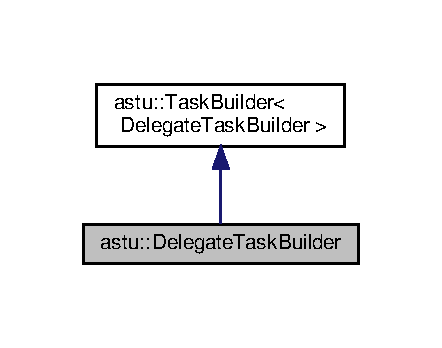
\includegraphics[width=212pt]{classastu_1_1DelegateTaskBuilder__inherit__graph}
\end{center}
\end{figure}


Collaboration diagram for astu\+:\+:Delegate\+Task\+Builder\+:\nopagebreak
\begin{figure}[H]
\begin{center}
\leavevmode
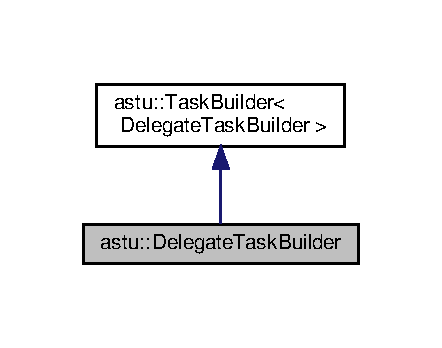
\includegraphics[width=212pt]{classastu_1_1DelegateTaskBuilder__coll__graph}
\end{center}
\end{figure}
\subsection*{Public Member Functions}
\begin{DoxyCompactItemize}
\item 
\hyperlink{classastu_1_1DelegateTaskBuilder_ab157afb8138680c515613b4296a7d665}{Delegate\+Task\+Builder} ()
\item 
\hyperlink{classastu_1_1DelegateTaskBuilder}{Delegate\+Task\+Builder} \& \hyperlink{classastu_1_1DelegateTaskBuilder_a40b80e0c6b20c1d6ea04a1c001f34dd2}{Delegate} (\hyperlink{classastu_1_1DelegateTask_a74c7859178eb0889e884209d1604de4d}{Delegate\+Task\+::\+Delegate} delegate)
\item 
\hyperlink{classastu_1_1DelegateTask_a74c7859178eb0889e884209d1604de4d}{Delegate\+Task\+::\+Delegate} \hyperlink{classastu_1_1DelegateTaskBuilder_abcbf0e7dbc8e4eed11a1214a266627ea}{Get\+Delegate} () const
\item 
\hyperlink{classastu_1_1DelegateTaskBuilder}{Delegate\+Task\+Builder} \& \hyperlink{classastu_1_1DelegateTaskBuilder_afff9f95d05d896a74935287e087eb2c4}{Delay} (double delay)
\item 
double \hyperlink{classastu_1_1DelegateTaskBuilder_a34340f7e709dea5c18aa4f4718e1bc79}{Get\+Delay} () const
\item 
\hyperlink{classastu_1_1DelegateTaskBuilder}{Delegate\+Task\+Builder} \& \hyperlink{classastu_1_1DelegateTaskBuilder_ad871e5e55e2d17fae9ae8503c179fc8f}{Reset} ()
\item 
std\+::unique\+\_\+ptr$<$ \hyperlink{classastu_1_1DelegateTask}{Delegate\+Task} $>$ \hyperlink{classastu_1_1DelegateTaskBuilder_a381daaf1473172b912ffe84da830c75c}{Build} ()
\end{DoxyCompactItemize}
\subsection*{Additional Inherited Members}


\subsection{Detailed Description}
Builder for \hyperlink{classastu_1_1DelegateTask}{Delegate\+Task} instances. 

\subsection{Constructor \& Destructor Documentation}
\mbox{\Hypertarget{classastu_1_1DelegateTaskBuilder_ab157afb8138680c515613b4296a7d665}\label{classastu_1_1DelegateTaskBuilder_ab157afb8138680c515613b4296a7d665}} 
\index{astu\+::\+Delegate\+Task\+Builder@{astu\+::\+Delegate\+Task\+Builder}!Delegate\+Task\+Builder@{Delegate\+Task\+Builder}}
\index{Delegate\+Task\+Builder@{Delegate\+Task\+Builder}!astu\+::\+Delegate\+Task\+Builder@{astu\+::\+Delegate\+Task\+Builder}}
\subsubsection{\texorpdfstring{Delegate\+Task\+Builder()}{DelegateTaskBuilder()}}
{\footnotesize\ttfamily astu\+::\+Delegate\+Task\+Builder\+::\+Delegate\+Task\+Builder (\begin{DoxyParamCaption}{ }\end{DoxyParamCaption})}

Constructor. 

\subsection{Member Function Documentation}
\mbox{\Hypertarget{classastu_1_1DelegateTaskBuilder_a381daaf1473172b912ffe84da830c75c}\label{classastu_1_1DelegateTaskBuilder_a381daaf1473172b912ffe84da830c75c}} 
\index{astu\+::\+Delegate\+Task\+Builder@{astu\+::\+Delegate\+Task\+Builder}!Build@{Build}}
\index{Build@{Build}!astu\+::\+Delegate\+Task\+Builder@{astu\+::\+Delegate\+Task\+Builder}}
\subsubsection{\texorpdfstring{Build()}{Build()}}
{\footnotesize\ttfamily std\+::unique\+\_\+ptr$<$\hyperlink{classastu_1_1DelegateTask}{Delegate\+Task}$>$ astu\+::\+Delegate\+Task\+Builder\+::\+Build (\begin{DoxyParamCaption}{ }\end{DoxyParamCaption})}

Builds a delegate task according to the current configuration.

\begin{DoxyReturn}{Returns}
the newly created delegate task 
\end{DoxyReturn}
\mbox{\Hypertarget{classastu_1_1DelegateTaskBuilder_afff9f95d05d896a74935287e087eb2c4}\label{classastu_1_1DelegateTaskBuilder_afff9f95d05d896a74935287e087eb2c4}} 
\index{astu\+::\+Delegate\+Task\+Builder@{astu\+::\+Delegate\+Task\+Builder}!Delay@{Delay}}
\index{Delay@{Delay}!astu\+::\+Delegate\+Task\+Builder@{astu\+::\+Delegate\+Task\+Builder}}
\subsubsection{\texorpdfstring{Delay()}{Delay()}}
{\footnotesize\ttfamily \hyperlink{classastu_1_1DelegateTaskBuilder}{Delegate\+Task\+Builder}\& astu\+::\+Delegate\+Task\+Builder\+::\+Delay (\begin{DoxyParamCaption}\item[{double}]{delay }\end{DoxyParamCaption})}

Specifies the delay for the delegate task to build.


\begin{DoxyParams}{Parameters}
{\em delay} & the delay in seconds \\
\hline
\end{DoxyParams}
\begin{DoxyReturn}{Returns}
reference to this builder for method chaining 
\end{DoxyReturn}
\mbox{\Hypertarget{classastu_1_1DelegateTaskBuilder_a40b80e0c6b20c1d6ea04a1c001f34dd2}\label{classastu_1_1DelegateTaskBuilder_a40b80e0c6b20c1d6ea04a1c001f34dd2}} 
\index{astu\+::\+Delegate\+Task\+Builder@{astu\+::\+Delegate\+Task\+Builder}!Delegate@{Delegate}}
\index{Delegate@{Delegate}!astu\+::\+Delegate\+Task\+Builder@{astu\+::\+Delegate\+Task\+Builder}}
\subsubsection{\texorpdfstring{Delegate()}{Delegate()}}
{\footnotesize\ttfamily \hyperlink{classastu_1_1DelegateTaskBuilder}{Delegate\+Task\+Builder}\& astu\+::\+Delegate\+Task\+Builder\+::\+Delegate (\begin{DoxyParamCaption}\item[{\hyperlink{classastu_1_1DelegateTask_a74c7859178eb0889e884209d1604de4d}{Delegate\+Task\+::\+Delegate}}]{delegate }\end{DoxyParamCaption})}

Specifies the delegate to be called by the task to build.


\begin{DoxyParams}{Parameters}
{\em delegate} & the delegate function \\
\hline
\end{DoxyParams}
\begin{DoxyReturn}{Returns}
reference to this builder for method chaining 
\end{DoxyReturn}
\mbox{\Hypertarget{classastu_1_1DelegateTaskBuilder_a34340f7e709dea5c18aa4f4718e1bc79}\label{classastu_1_1DelegateTaskBuilder_a34340f7e709dea5c18aa4f4718e1bc79}} 
\index{astu\+::\+Delegate\+Task\+Builder@{astu\+::\+Delegate\+Task\+Builder}!Get\+Delay@{Get\+Delay}}
\index{Get\+Delay@{Get\+Delay}!astu\+::\+Delegate\+Task\+Builder@{astu\+::\+Delegate\+Task\+Builder}}
\subsubsection{\texorpdfstring{Get\+Delay()}{GetDelay()}}
{\footnotesize\ttfamily double astu\+::\+Delegate\+Task\+Builder\+::\+Get\+Delay (\begin{DoxyParamCaption}{ }\end{DoxyParamCaption}) const\hspace{0.3cm}{\ttfamily [inline]}}

Returns the delay used for the task to build.
\begin{DoxyItemize}
\item \begin{DoxyReturn}{Returns}
the delay in seconds 
\end{DoxyReturn}

\end{DoxyItemize}\mbox{\Hypertarget{classastu_1_1DelegateTaskBuilder_abcbf0e7dbc8e4eed11a1214a266627ea}\label{classastu_1_1DelegateTaskBuilder_abcbf0e7dbc8e4eed11a1214a266627ea}} 
\index{astu\+::\+Delegate\+Task\+Builder@{astu\+::\+Delegate\+Task\+Builder}!Get\+Delegate@{Get\+Delegate}}
\index{Get\+Delegate@{Get\+Delegate}!astu\+::\+Delegate\+Task\+Builder@{astu\+::\+Delegate\+Task\+Builder}}
\subsubsection{\texorpdfstring{Get\+Delegate()}{GetDelegate()}}
{\footnotesize\ttfamily \hyperlink{classastu_1_1DelegateTask_a74c7859178eb0889e884209d1604de4d}{Delegate\+Task\+::\+Delegate} astu\+::\+Delegate\+Task\+Builder\+::\+Get\+Delegate (\begin{DoxyParamCaption}{ }\end{DoxyParamCaption}) const\hspace{0.3cm}{\ttfamily [inline]}}

Returns the delegate used for the task to build.
\begin{DoxyItemize}
\item \begin{DoxyReturn}{Returns}
the delegate 
\end{DoxyReturn}

\end{DoxyItemize}\mbox{\Hypertarget{classastu_1_1DelegateTaskBuilder_ad871e5e55e2d17fae9ae8503c179fc8f}\label{classastu_1_1DelegateTaskBuilder_ad871e5e55e2d17fae9ae8503c179fc8f}} 
\index{astu\+::\+Delegate\+Task\+Builder@{astu\+::\+Delegate\+Task\+Builder}!Reset@{Reset}}
\index{Reset@{Reset}!astu\+::\+Delegate\+Task\+Builder@{astu\+::\+Delegate\+Task\+Builder}}
\subsubsection{\texorpdfstring{Reset()}{Reset()}}
{\footnotesize\ttfamily \hyperlink{classastu_1_1DelegateTaskBuilder}{Delegate\+Task\+Builder}\& astu\+::\+Delegate\+Task\+Builder\+::\+Reset (\begin{DoxyParamCaption}{ }\end{DoxyParamCaption})}

Resets this builder to is initial configuration.

\begin{DoxyReturn}{Returns}
reference to this builder for method chaining 
\end{DoxyReturn}


The documentation for this class was generated from the following file\+:\begin{DoxyCompactItemize}
\item 
include/\+Service/Tasks.\+h\end{DoxyCompactItemize}

\hypertarget{classastu_1_1Entity}{}\section{astu\+:\+:Entity Class Reference}
\label{classastu_1_1Entity}\index{astu\+::\+Entity@{astu\+::\+Entity}}


{\ttfamily \#include $<$Entity\+Service.\+h$>$}



Inheritance diagram for astu\+:\+:Entity\+:\nopagebreak
\begin{figure}[H]
\begin{center}
\leavevmode
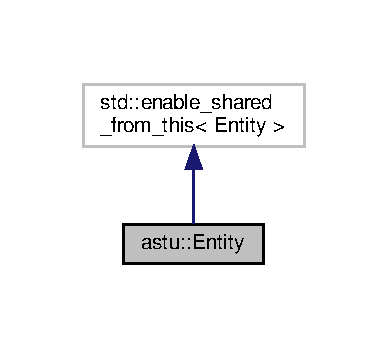
\includegraphics[width=186pt]{classastu_1_1Entity__inherit__graph}
\end{center}
\end{figure}


Collaboration diagram for astu\+:\+:Entity\+:\nopagebreak
\begin{figure}[H]
\begin{center}
\leavevmode
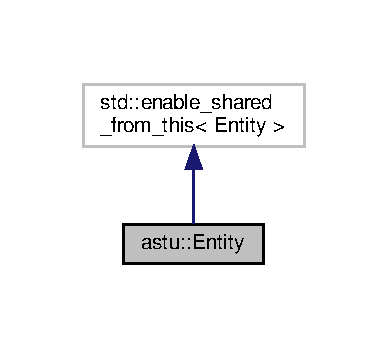
\includegraphics[width=186pt]{classastu_1_1Entity__coll__graph}
\end{center}
\end{figure}
\subsection*{Public Member Functions}
\begin{DoxyCompactItemize}
\item 
\hyperlink{classastu_1_1Entity_aed9aac4a995b5c044c0301302f2bd3d0}{Entity} ()
\item 
void \hyperlink{classastu_1_1Entity_ab8f47f4de88139f9202466b726e61aee}{Add\+Component} (std\+::shared\+\_\+ptr$<$ \hyperlink{classastu_1_1EntityComponent}{Entity\+Component} $>$ cmp)
\item 
bool \hyperlink{classastu_1_1Entity_ad1ee4a4e617de7c40eb252413b9045a1}{Has\+Component} (const std\+::type\+\_\+index \&type) const
\item 
\hyperlink{classastu_1_1EntityComponent}{Entity\+Component} \& \hyperlink{classastu_1_1Entity_a3d9bb583859f1a941fdaad76f5093323}{Get\+Component} (const std\+::type\+\_\+index \&type)
\item 
const \hyperlink{classastu_1_1EntityComponent}{Entity\+Component} \& \hyperlink{classastu_1_1Entity_affe49f8c35d5b067f06803e27243189a}{Get\+Component} (const std\+::type\+\_\+index \&type) const
\item 
{\footnotesize template$<$typename T $>$ }\\T \& \hyperlink{classastu_1_1Entity_aeabb500a719de29039dd0fad4ea553c4}{Get\+Component} ()
\item 
{\footnotesize template$<$typename T $>$ }\\bool \hyperlink{classastu_1_1Entity_a80b75df1873d23f79f050bc6a178cd4c}{Has\+Component} ()
\end{DoxyCompactItemize}


\subsection{Detailed Description}
An entity is a container for compoments. 

\subsection{Constructor \& Destructor Documentation}
\mbox{\Hypertarget{classastu_1_1Entity_aed9aac4a995b5c044c0301302f2bd3d0}\label{classastu_1_1Entity_aed9aac4a995b5c044c0301302f2bd3d0}} 
\index{astu\+::\+Entity@{astu\+::\+Entity}!Entity@{Entity}}
\index{Entity@{Entity}!astu\+::\+Entity@{astu\+::\+Entity}}
\subsubsection{\texorpdfstring{Entity()}{Entity()}}
{\footnotesize\ttfamily astu\+::\+Entity\+::\+Entity (\begin{DoxyParamCaption}{ }\end{DoxyParamCaption})\hspace{0.3cm}{\ttfamily [inline]}}

Constructor. 

\subsection{Member Function Documentation}
\mbox{\Hypertarget{classastu_1_1Entity_ab8f47f4de88139f9202466b726e61aee}\label{classastu_1_1Entity_ab8f47f4de88139f9202466b726e61aee}} 
\index{astu\+::\+Entity@{astu\+::\+Entity}!Add\+Component@{Add\+Component}}
\index{Add\+Component@{Add\+Component}!astu\+::\+Entity@{astu\+::\+Entity}}
\subsubsection{\texorpdfstring{Add\+Component()}{AddComponent()}}
{\footnotesize\ttfamily void astu\+::\+Entity\+::\+Add\+Component (\begin{DoxyParamCaption}\item[{std\+::shared\+\_\+ptr$<$ \hyperlink{classastu_1_1EntityComponent}{Entity\+Component} $>$}]{cmp }\end{DoxyParamCaption})}

Adds a component to this entity.


\begin{DoxyParams}{Parameters}
{\em cmp} & the component to add \\
\hline
\end{DoxyParams}
\mbox{\Hypertarget{classastu_1_1Entity_a3d9bb583859f1a941fdaad76f5093323}\label{classastu_1_1Entity_a3d9bb583859f1a941fdaad76f5093323}} 
\index{astu\+::\+Entity@{astu\+::\+Entity}!Get\+Component@{Get\+Component}}
\index{Get\+Component@{Get\+Component}!astu\+::\+Entity@{astu\+::\+Entity}}
\subsubsection{\texorpdfstring{Get\+Component()}{GetComponent()}\hspace{0.1cm}{\footnotesize\ttfamily [1/3]}}
{\footnotesize\ttfamily \hyperlink{classastu_1_1EntityComponent}{Entity\+Component}\& astu\+::\+Entity\+::\+Get\+Component (\begin{DoxyParamCaption}\item[{const std\+::type\+\_\+index \&}]{type }\end{DoxyParamCaption})}

Returns the component of a specific type.

This method is mainly used by the template method {\ttfamily get\+Component}, which is much more convenient to use because no type cast is required.

A dynamic cast is not necessary because this method ensures to return a component of the required type which can safely be casted using a fast static cast.

{\bfseries Usage example\+:} 
\begin{DoxyCode}
\textcolor{keyword}{auto} & pose = \textcolor{keyword}{static\_cast<}Pose2D &\textcolor{keyword}{>}( entity.getComponent( std::type\_index( \textcolor{keyword}{typeid}(Pose2D) ) ) );
\end{DoxyCode}



\begin{DoxyParams}{Parameters}
{\em type} & the component type \\
\hline
\end{DoxyParams}
\begin{DoxyReturn}{Returns}
the requested component 
\end{DoxyReturn}

\begin{DoxyExceptions}{Exceptions}
{\em std\+::logic\+\_\+error} & in case the requested component does not exist \\
\hline
\end{DoxyExceptions}
\mbox{\Hypertarget{classastu_1_1Entity_affe49f8c35d5b067f06803e27243189a}\label{classastu_1_1Entity_affe49f8c35d5b067f06803e27243189a}} 
\index{astu\+::\+Entity@{astu\+::\+Entity}!Get\+Component@{Get\+Component}}
\index{Get\+Component@{Get\+Component}!astu\+::\+Entity@{astu\+::\+Entity}}
\subsubsection{\texorpdfstring{Get\+Component()}{GetComponent()}\hspace{0.1cm}{\footnotesize\ttfamily [2/3]}}
{\footnotesize\ttfamily const \hyperlink{classastu_1_1EntityComponent}{Entity\+Component}\& astu\+::\+Entity\+::\+Get\+Component (\begin{DoxyParamCaption}\item[{const std\+::type\+\_\+index \&}]{type }\end{DoxyParamCaption}) const}

Returns the component of a specific type.

This is the constant version of this method. See the non-\/constant version description for details.


\begin{DoxyParams}{Parameters}
{\em type} & the component type \\
\hline
\end{DoxyParams}
\begin{DoxyReturn}{Returns}
the requested component 
\end{DoxyReturn}

\begin{DoxyExceptions}{Exceptions}
{\em std\+::logic\+\_\+error} & in case the requested component does not exist \\
\hline
\end{DoxyExceptions}
\mbox{\Hypertarget{classastu_1_1Entity_aeabb500a719de29039dd0fad4ea553c4}\label{classastu_1_1Entity_aeabb500a719de29039dd0fad4ea553c4}} 
\index{astu\+::\+Entity@{astu\+::\+Entity}!Get\+Component@{Get\+Component}}
\index{Get\+Component@{Get\+Component}!astu\+::\+Entity@{astu\+::\+Entity}}
\subsubsection{\texorpdfstring{Get\+Component()}{GetComponent()}\hspace{0.1cm}{\footnotesize\ttfamily [3/3]}}
{\footnotesize\ttfamily template$<$typename T $>$ \\
T\& astu\+::\+Entity\+::\+Get\+Component (\begin{DoxyParamCaption}{ }\end{DoxyParamCaption})\hspace{0.3cm}{\ttfamily [inline]}}

Retrieves the component a specifi type from this entity.

This template method offers a convenient way to retrieve a component by specifying the type of the component to retrieve as template parameter.

{\bfseries Usage example\+:} 
\begin{DoxyCode}
\textcolor{keyword}{auto} & pose = entity.getComponent<Pose2D>();
\end{DoxyCode}



\begin{DoxyTemplParams}{Template Parameters}
{\em T} & the type of the component to retrieve \\
\hline
\end{DoxyTemplParams}
\begin{DoxyReturn}{Returns}
the requested component 
\end{DoxyReturn}

\begin{DoxyExceptions}{Exceptions}
{\em std\+::logic\+\_\+error} & in case the requested component does not exist \\
\hline
\end{DoxyExceptions}
\mbox{\Hypertarget{classastu_1_1Entity_ad1ee4a4e617de7c40eb252413b9045a1}\label{classastu_1_1Entity_ad1ee4a4e617de7c40eb252413b9045a1}} 
\index{astu\+::\+Entity@{astu\+::\+Entity}!Has\+Component@{Has\+Component}}
\index{Has\+Component@{Has\+Component}!astu\+::\+Entity@{astu\+::\+Entity}}
\subsubsection{\texorpdfstring{Has\+Component()}{HasComponent()}\hspace{0.1cm}{\footnotesize\ttfamily [1/2]}}
{\footnotesize\ttfamily bool astu\+::\+Entity\+::\+Has\+Component (\begin{DoxyParamCaption}\item[{const std\+::type\+\_\+index \&}]{type }\end{DoxyParamCaption}) const}

Tests if specified type of component has been added to this entity.

This method is mainly used by the template method {\ttfamily Has\+Component}, which is more convenient to use.

This method requires a std\+::type\+\_\+index parameter to specify the type of component to be tested. The C++ {\ttfamily typeid} operator can be used to get the std\+::type\+\_\+info object, which will be automatically converted to a std\+::type\+\_\+index object when calling this method.

{\bfseries Usage example\+:} 
\begin{DoxyCode}
\textcolor{keywordflow}{if} ( entity.hasComponent( \textcolor{keyword}{typeid}(Pose2D) ) ) \{
    \textcolor{comment}{// do something with Pose2D component}
\}
\end{DoxyCode}



\begin{DoxyParams}{Parameters}
{\em type} & a type\+\_\+index specifying the type of component to test \\
\hline
\end{DoxyParams}
\begin{DoxyReturn}{Returns}
{\ttfamily true} if a component of the specified type exists 
\end{DoxyReturn}
\mbox{\Hypertarget{classastu_1_1Entity_a80b75df1873d23f79f050bc6a178cd4c}\label{classastu_1_1Entity_a80b75df1873d23f79f050bc6a178cd4c}} 
\index{astu\+::\+Entity@{astu\+::\+Entity}!Has\+Component@{Has\+Component}}
\index{Has\+Component@{Has\+Component}!astu\+::\+Entity@{astu\+::\+Entity}}
\subsubsection{\texorpdfstring{Has\+Component()}{HasComponent()}\hspace{0.1cm}{\footnotesize\ttfamily [2/2]}}
{\footnotesize\ttfamily template$<$typename T $>$ \\
bool astu\+::\+Entity\+::\+Has\+Component (\begin{DoxyParamCaption}{ }\end{DoxyParamCaption})\hspace{0.3cm}{\ttfamily [inline]}}

Tests whether a component of a specific type has been added to this entity.

This template method offers a convenient way to test if a certain component type exists in this entity by specifying the type of the component as template parameter.

{\bfseries Usage example\+:} 
\begin{DoxyCode}
\textcolor{keywordflow}{if} ( entity.hasComponent<Pose2D>() ) \{
    \textcolor{comment}{// do something with Pose2D component}
\}
\end{DoxyCode}



\begin{DoxyTemplParams}{Template Parameters}
{\em T} & the type of component to be tested \\
\hline
\end{DoxyTemplParams}
\begin{DoxyReturn}{Returns}
{\ttfamily true} if a component of the specified type exists 
\end{DoxyReturn}


The documentation for this class was generated from the following file\+:\begin{DoxyCompactItemize}
\item 
include/Entity\+Service.\+h\end{DoxyCompactItemize}

\hypertarget{classastu_1_1EntityComponent}{}\section{astu\+:\+:Entity\+Component Class Reference}
\label{classastu_1_1EntityComponent}\index{astu\+::\+Entity\+Component@{astu\+::\+Entity\+Component}}


{\ttfamily \#include $<$Entity\+Service.\+h$>$}

\subsection*{Public Member Functions}
\begin{DoxyCompactItemize}
\item 
\hyperlink{classastu_1_1EntityComponent_a9bb95d7ddc55093fd86e04d5b6aa98ec}{Entity\+Component} ()=default
\item 
virtual \hyperlink{classastu_1_1EntityComponent_a17295f763e201247c22bc677541646e5}{$\sim$\+Entity\+Component} ()
\end{DoxyCompactItemize}


\subsection{Detailed Description}
Base class for all entity components. 

\subsection{Constructor \& Destructor Documentation}
\mbox{\Hypertarget{classastu_1_1EntityComponent_a9bb95d7ddc55093fd86e04d5b6aa98ec}\label{classastu_1_1EntityComponent_a9bb95d7ddc55093fd86e04d5b6aa98ec}} 
\index{astu\+::\+Entity\+Component@{astu\+::\+Entity\+Component}!Entity\+Component@{Entity\+Component}}
\index{Entity\+Component@{Entity\+Component}!astu\+::\+Entity\+Component@{astu\+::\+Entity\+Component}}
\subsubsection{\texorpdfstring{Entity\+Component()}{EntityComponent()}}
{\footnotesize\ttfamily astu\+::\+Entity\+Component\+::\+Entity\+Component (\begin{DoxyParamCaption}{ }\end{DoxyParamCaption})\hspace{0.3cm}{\ttfamily [default]}}

Constructor. \mbox{\Hypertarget{classastu_1_1EntityComponent_a17295f763e201247c22bc677541646e5}\label{classastu_1_1EntityComponent_a17295f763e201247c22bc677541646e5}} 
\index{astu\+::\+Entity\+Component@{astu\+::\+Entity\+Component}!````~Entity\+Component@{$\sim$\+Entity\+Component}}
\index{````~Entity\+Component@{$\sim$\+Entity\+Component}!astu\+::\+Entity\+Component@{astu\+::\+Entity\+Component}}
\subsubsection{\texorpdfstring{$\sim$\+Entity\+Component()}{~EntityComponent()}}
{\footnotesize\ttfamily virtual astu\+::\+Entity\+Component\+::$\sim$\+Entity\+Component (\begin{DoxyParamCaption}{ }\end{DoxyParamCaption})\hspace{0.3cm}{\ttfamily [inline]}, {\ttfamily [virtual]}}

Virtual destructor. 

The documentation for this class was generated from the following file\+:\begin{DoxyCompactItemize}
\item 
include/Entity\+Service.\+h\end{DoxyCompactItemize}

\hypertarget{classastu_1_1EntityFactoryService}{}\section{astu\+:\+:Entity\+Factory\+Service Class Reference}
\label{classastu_1_1EntityFactoryService}\index{astu\+::\+Entity\+Factory\+Service@{astu\+::\+Entity\+Factory\+Service}}


{\ttfamily \#include $<$Entity\+Factory\+Service.\+h$>$}



Inheritance diagram for astu\+:\+:Entity\+Factory\+Service\+:\nopagebreak
\begin{figure}[H]
\begin{center}
\leavevmode
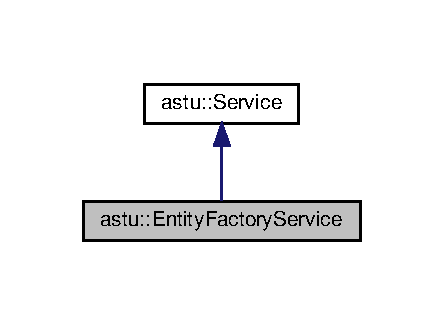
\includegraphics[width=213pt]{classastu_1_1EntityFactoryService__inherit__graph}
\end{center}
\end{figure}


Collaboration diagram for astu\+:\+:Entity\+Factory\+Service\+:\nopagebreak
\begin{figure}[H]
\begin{center}
\leavevmode
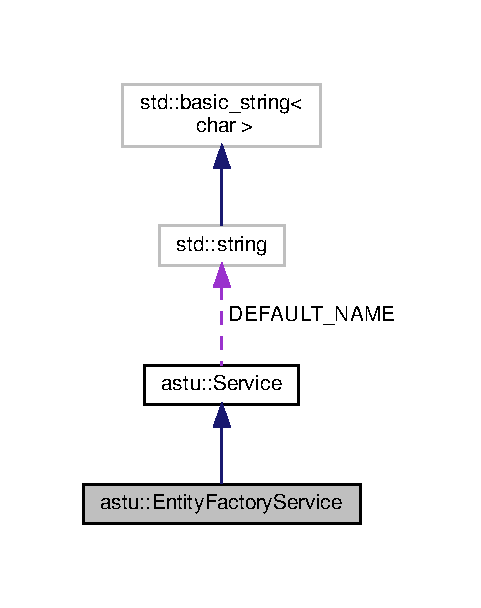
\includegraphics[width=231pt]{classastu_1_1EntityFactoryService__coll__graph}
\end{center}
\end{figure}
\subsection*{Public Member Functions}
\begin{DoxyCompactItemize}
\item 
\hyperlink{classastu_1_1EntityFactoryService_a7b88d3c794298156e1aacd60cc25e818}{Entity\+Factory\+Service} ()
\item 
bool \hyperlink{classastu_1_1EntityFactoryService_aa1b33aaf444b5d42e774522f0862df4a}{Has\+Prototype} (const std\+::string \&proto\+Name) const
\item 
void \hyperlink{classastu_1_1EntityFactoryService_ade1d8c60a6982c409501e58dcd8c2bc8}{Register\+Prototype} (const std\+::string \&proto\+Name, std\+::shared\+\_\+ptr$<$ \hyperlink{classastu_1_1Entity}{Entity} $>$ proto)
\item 
void \hyperlink{classastu_1_1EntityFactoryService_a0256f46b4344c1f66d1d6ed947992c62}{Deregister\+Prototype} (const std\+::string \&proto\+Name)
\item 
void \hyperlink{classastu_1_1EntityFactoryService_a2ffee25bef45ed4b845dd2b9c852496d}{Deregister\+All\+Prototypes} ()
\item 
std\+::shared\+\_\+ptr$<$ \hyperlink{classastu_1_1Entity}{Entity} $>$ \hyperlink{classastu_1_1EntityFactoryService_aef424f6a70cbc918bea4a7edd738877f}{Create\+Entity} (const std\+::string \&proto\+Name) const
\end{DoxyCompactItemize}
\subsection*{Additional Inherited Members}


\subsection{Detailed Description}
This entity factory is used to generate new entities, where entities are defined by prototypes that are cloned when new entities are created. 

\subsection{Constructor \& Destructor Documentation}
\mbox{\Hypertarget{classastu_1_1EntityFactoryService_a7b88d3c794298156e1aacd60cc25e818}\label{classastu_1_1EntityFactoryService_a7b88d3c794298156e1aacd60cc25e818}} 
\index{astu\+::\+Entity\+Factory\+Service@{astu\+::\+Entity\+Factory\+Service}!Entity\+Factory\+Service@{Entity\+Factory\+Service}}
\index{Entity\+Factory\+Service@{Entity\+Factory\+Service}!astu\+::\+Entity\+Factory\+Service@{astu\+::\+Entity\+Factory\+Service}}
\subsubsection{\texorpdfstring{Entity\+Factory\+Service()}{EntityFactoryService()}}
{\footnotesize\ttfamily astu\+::\+Entity\+Factory\+Service\+::\+Entity\+Factory\+Service (\begin{DoxyParamCaption}{ }\end{DoxyParamCaption})}

Constructor. 

\subsection{Member Function Documentation}
\mbox{\Hypertarget{classastu_1_1EntityFactoryService_aef424f6a70cbc918bea4a7edd738877f}\label{classastu_1_1EntityFactoryService_aef424f6a70cbc918bea4a7edd738877f}} 
\index{astu\+::\+Entity\+Factory\+Service@{astu\+::\+Entity\+Factory\+Service}!Create\+Entity@{Create\+Entity}}
\index{Create\+Entity@{Create\+Entity}!astu\+::\+Entity\+Factory\+Service@{astu\+::\+Entity\+Factory\+Service}}
\subsubsection{\texorpdfstring{Create\+Entity()}{CreateEntity()}}
{\footnotesize\ttfamily std\+::shared\+\_\+ptr$<$\hyperlink{classastu_1_1Entity}{Entity}$>$ astu\+::\+Entity\+Factory\+Service\+::\+Create\+Entity (\begin{DoxyParamCaption}\item[{const std\+::string \&}]{proto\+Name }\end{DoxyParamCaption}) const}

Creates a new entity based on a registered prototype.


\begin{DoxyParams}{Parameters}
{\em proto\+Name} & the name of the prototype \\
\hline
\end{DoxyParams}

\begin{DoxyExceptions}{Exceptions}
{\em std\+::logic\+\_\+error} & in case the given name is unknown \\
\hline
\end{DoxyExceptions}
\mbox{\Hypertarget{classastu_1_1EntityFactoryService_a2ffee25bef45ed4b845dd2b9c852496d}\label{classastu_1_1EntityFactoryService_a2ffee25bef45ed4b845dd2b9c852496d}} 
\index{astu\+::\+Entity\+Factory\+Service@{astu\+::\+Entity\+Factory\+Service}!Deregister\+All\+Prototypes@{Deregister\+All\+Prototypes}}
\index{Deregister\+All\+Prototypes@{Deregister\+All\+Prototypes}!astu\+::\+Entity\+Factory\+Service@{astu\+::\+Entity\+Factory\+Service}}
\subsubsection{\texorpdfstring{Deregister\+All\+Prototypes()}{DeregisterAllPrototypes()}}
{\footnotesize\ttfamily void astu\+::\+Entity\+Factory\+Service\+::\+Deregister\+All\+Prototypes (\begin{DoxyParamCaption}{ }\end{DoxyParamCaption})}

Deregisters all prototypes. \mbox{\Hypertarget{classastu_1_1EntityFactoryService_a0256f46b4344c1f66d1d6ed947992c62}\label{classastu_1_1EntityFactoryService_a0256f46b4344c1f66d1d6ed947992c62}} 
\index{astu\+::\+Entity\+Factory\+Service@{astu\+::\+Entity\+Factory\+Service}!Deregister\+Prototype@{Deregister\+Prototype}}
\index{Deregister\+Prototype@{Deregister\+Prototype}!astu\+::\+Entity\+Factory\+Service@{astu\+::\+Entity\+Factory\+Service}}
\subsubsection{\texorpdfstring{Deregister\+Prototype()}{DeregisterPrototype()}}
{\footnotesize\ttfamily void astu\+::\+Entity\+Factory\+Service\+::\+Deregister\+Prototype (\begin{DoxyParamCaption}\item[{const std\+::string \&}]{proto\+Name }\end{DoxyParamCaption})}

Deregisters an entityentity prototype.


\begin{DoxyParams}{Parameters}
{\em proto\+Name} & the name of the prototype \\
\hline
\end{DoxyParams}
\mbox{\Hypertarget{classastu_1_1EntityFactoryService_aa1b33aaf444b5d42e774522f0862df4a}\label{classastu_1_1EntityFactoryService_aa1b33aaf444b5d42e774522f0862df4a}} 
\index{astu\+::\+Entity\+Factory\+Service@{astu\+::\+Entity\+Factory\+Service}!Has\+Prototype@{Has\+Prototype}}
\index{Has\+Prototype@{Has\+Prototype}!astu\+::\+Entity\+Factory\+Service@{astu\+::\+Entity\+Factory\+Service}}
\subsubsection{\texorpdfstring{Has\+Prototype()}{HasPrototype()}}
{\footnotesize\ttfamily bool astu\+::\+Entity\+Factory\+Service\+::\+Has\+Prototype (\begin{DoxyParamCaption}\item[{const std\+::string \&}]{proto\+Name }\end{DoxyParamCaption}) const}

Tests whether a entity has been register.


\begin{DoxyParams}{Parameters}
{\em proto\+Name} & the name under which the entity has been registered \\
\hline
\end{DoxyParams}
\begin{DoxyReturn}{Returns}
{\ttfamily true} if an entity has been registered with the given name 
\end{DoxyReturn}
\mbox{\Hypertarget{classastu_1_1EntityFactoryService_ade1d8c60a6982c409501e58dcd8c2bc8}\label{classastu_1_1EntityFactoryService_ade1d8c60a6982c409501e58dcd8c2bc8}} 
\index{astu\+::\+Entity\+Factory\+Service@{astu\+::\+Entity\+Factory\+Service}!Register\+Prototype@{Register\+Prototype}}
\index{Register\+Prototype@{Register\+Prototype}!astu\+::\+Entity\+Factory\+Service@{astu\+::\+Entity\+Factory\+Service}}
\subsubsection{\texorpdfstring{Register\+Prototype()}{RegisterPrototype()}}
{\footnotesize\ttfamily void astu\+::\+Entity\+Factory\+Service\+::\+Register\+Prototype (\begin{DoxyParamCaption}\item[{const std\+::string \&}]{proto\+Name,  }\item[{std\+::shared\+\_\+ptr$<$ \hyperlink{classastu_1_1Entity}{Entity} $>$}]{proto }\end{DoxyParamCaption})}

Registers a new entity prototype.


\begin{DoxyParams}{Parameters}
{\em proto\+Name} & the name of the prototype \\
\hline
{\em proto} & the entity prototype \\
\hline
\end{DoxyParams}

\begin{DoxyExceptions}{Exceptions}
{\em std\+::logic\+\_\+error} & in case the given name is already used \\
\hline
\end{DoxyExceptions}


The documentation for this class was generated from the following file\+:\begin{DoxyCompactItemize}
\item 
include/\+E\+C\+S/Entity\+Factory\+Service.\+h\end{DoxyCompactItemize}

\hypertarget{classastu_1_1EntityFamily}{}\section{astu\+:\+:Entity\+Family Class Reference}
\label{classastu_1_1EntityFamily}\index{astu\+::\+Entity\+Family@{astu\+::\+Entity\+Family}}


{\ttfamily \#include $<$Entity\+Service.\+h$>$}

\subsection*{Public Member Functions}
\begin{DoxyCompactItemize}
\item 
\mbox{\Hypertarget{classastu_1_1EntityFamily_a8452fd5df3f194dd8824b9ea88d426bf}\label{classastu_1_1EntityFamily_a8452fd5df3f194dd8824b9ea88d426bf}} 
bool {\bfseries Is\+Member} (const \hyperlink{classastu_1_1Entity}{Entity} \&entity) const
\item 
bool \hyperlink{classastu_1_1EntityFamily_ac2389d2f9807b3ebdb570f0fd8930957}{operator$<$} (const \hyperlink{classastu_1_1EntityFamily}{Entity\+Family} \&o) const
\end{DoxyCompactItemize}
\subsection*{Static Public Member Functions}
\begin{DoxyCompactItemize}
\item 
{\footnotesize template$<$typename ... Ts$>$ }\\static \hyperlink{classastu_1_1EntityFamily}{Entity\+Family} \hyperlink{classastu_1_1EntityFamily_ad201d4186eaef0f02c07a07889fc7763}{Create} ()
\end{DoxyCompactItemize}


\subsection{Detailed Description}
Describes entities which share a certain set of entity components. 

\subsection{Member Function Documentation}
\mbox{\Hypertarget{classastu_1_1EntityFamily_ad201d4186eaef0f02c07a07889fc7763}\label{classastu_1_1EntityFamily_ad201d4186eaef0f02c07a07889fc7763}} 
\index{astu\+::\+Entity\+Family@{astu\+::\+Entity\+Family}!Create@{Create}}
\index{Create@{Create}!astu\+::\+Entity\+Family@{astu\+::\+Entity\+Family}}
\subsubsection{\texorpdfstring{Create()}{Create()}}
{\footnotesize\ttfamily template$<$typename ... Ts$>$ \\
static \hyperlink{classastu_1_1EntityFamily}{Entity\+Family} astu\+::\+Entity\+Family\+::\+Create (\begin{DoxyParamCaption}{ }\end{DoxyParamCaption})\hspace{0.3cm}{\ttfamily [inline]}, {\ttfamily [static]}}

Creates a new entity family. This static factory method is the only way to construct entity families. The constructor of this class is private.

Example usage\+: 
\begin{DoxyCode}
EntityFamily myFamily = EntityFamily::create<Transform2D, ShapeVisual2D>();
\end{DoxyCode}



\begin{DoxyTemplParams}{Template Parameters}
{\em Ts} & list of components the requested entities should share \\
\hline
\end{DoxyTemplParams}
\begin{DoxyReturn}{Returns}
the entity family 
\end{DoxyReturn}
\mbox{\Hypertarget{classastu_1_1EntityFamily_ac2389d2f9807b3ebdb570f0fd8930957}\label{classastu_1_1EntityFamily_ac2389d2f9807b3ebdb570f0fd8930957}} 
\index{astu\+::\+Entity\+Family@{astu\+::\+Entity\+Family}!operator$<$@{operator$<$}}
\index{operator$<$@{operator$<$}!astu\+::\+Entity\+Family@{astu\+::\+Entity\+Family}}
\subsubsection{\texorpdfstring{operator$<$()}{operator<()}}
{\footnotesize\ttfamily bool astu\+::\+Entity\+Family\+::operator$<$ (\begin{DoxyParamCaption}\item[{const \hyperlink{classastu_1_1EntityFamily}{Entity\+Family} \&}]{o }\end{DoxyParamCaption}) const\hspace{0.3cm}{\ttfamily [inline]}}

Binary less operator.

This operator is required to work as key in a map container. The less operator induces a strict weak ordering of elements.


\begin{DoxyParams}{Parameters}
{\em o} & the other entity family (right hand side) \\
\hline
\end{DoxyParams}
\begin{DoxyReturn}{Returns}
{\ttfamily true} if this element is less than the given element. 
\end{DoxyReturn}


The documentation for this class was generated from the following file\+:\begin{DoxyCompactItemize}
\item 
include/Entity\+Service.\+h\end{DoxyCompactItemize}

\hypertarget{classastu_1_1EntityListener}{}\section{astu\+:\+:Entity\+Listener Class Reference}
\label{classastu_1_1EntityListener}\index{astu\+::\+Entity\+Listener@{astu\+::\+Entity\+Listener}}


{\ttfamily \#include $<$Entity\+Systems.\+h$>$}



Inheritance diagram for astu\+:\+:Entity\+Listener\+:\nopagebreak
\begin{figure}[H]
\begin{center}
\leavevmode
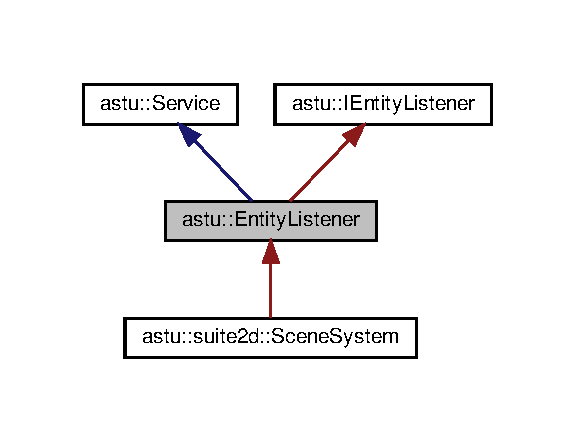
\includegraphics[width=276pt]{classastu_1_1EntityListener__inherit__graph}
\end{center}
\end{figure}


Collaboration diagram for astu\+:\+:Entity\+Listener\+:\nopagebreak
\begin{figure}[H]
\begin{center}
\leavevmode
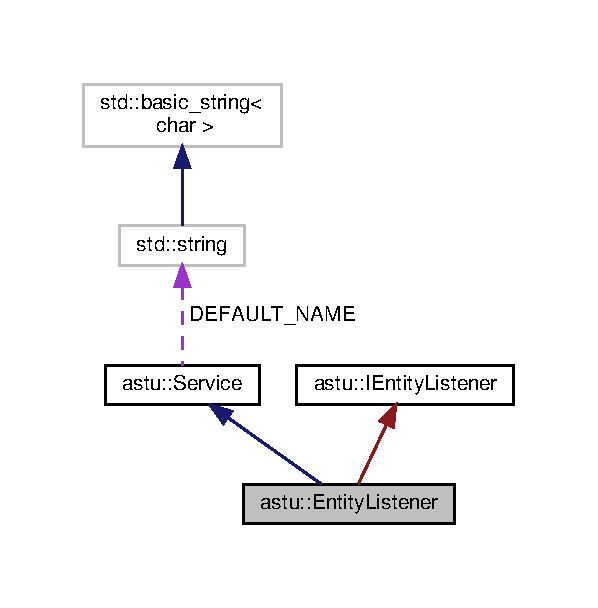
\includegraphics[width=287pt]{classastu_1_1EntityListener__coll__graph}
\end{center}
\end{figure}
\subsection*{Public Member Functions}
\begin{DoxyCompactItemize}
\item 
\hyperlink{classastu_1_1EntityListener_a16450ccf235ecd96db0f62e6bed7bb07}{Entity\+Listener} (const \hyperlink{classastu_1_1EntityFamily}{Entity\+Family} \&family)
\item 
virtual void \hyperlink{classastu_1_1EntityListener_a0c123b57dcabc4c2b6cee8f05db545c8}{On\+Entity\+Added} (std\+::shared\+\_\+ptr$<$ \hyperlink{classastu_1_1Entity}{astu\+::\+Entity} $>$ entity) override
\item 
virtual void \hyperlink{classastu_1_1EntityListener_ae380d941fafd6933a9f290ac50e7f32b}{On\+Entity\+Removed} (std\+::shared\+\_\+ptr$<$ \hyperlink{classastu_1_1Entity}{astu\+::\+Entity} $>$ entity) override
\end{DoxyCompactItemize}
\subsection*{Additional Inherited Members}


\subsection{Detailed Description}
Services can derive from this class to get informed when an entity of a certain family is added or remove to the entity service. 

\subsection{Constructor \& Destructor Documentation}
\mbox{\Hypertarget{classastu_1_1EntityListener_a16450ccf235ecd96db0f62e6bed7bb07}\label{classastu_1_1EntityListener_a16450ccf235ecd96db0f62e6bed7bb07}} 
\index{astu\+::\+Entity\+Listener@{astu\+::\+Entity\+Listener}!Entity\+Listener@{Entity\+Listener}}
\index{Entity\+Listener@{Entity\+Listener}!astu\+::\+Entity\+Listener@{astu\+::\+Entity\+Listener}}
\subsubsection{\texorpdfstring{Entity\+Listener()}{EntityListener()}}
{\footnotesize\ttfamily astu\+::\+Entity\+Listener\+::\+Entity\+Listener (\begin{DoxyParamCaption}\item[{const \hyperlink{classastu_1_1EntityFamily}{Entity\+Family} \&}]{family }\end{DoxyParamCaption})\hspace{0.3cm}{\ttfamily [inline]}}

Constructor.


\begin{DoxyParams}{Parameters}
{\em family} & the family of entities this system processes \\
\hline
\end{DoxyParams}


\subsection{Member Function Documentation}
\mbox{\Hypertarget{classastu_1_1EntityListener_a0c123b57dcabc4c2b6cee8f05db545c8}\label{classastu_1_1EntityListener_a0c123b57dcabc4c2b6cee8f05db545c8}} 
\index{astu\+::\+Entity\+Listener@{astu\+::\+Entity\+Listener}!On\+Entity\+Added@{On\+Entity\+Added}}
\index{On\+Entity\+Added@{On\+Entity\+Added}!astu\+::\+Entity\+Listener@{astu\+::\+Entity\+Listener}}
\subsubsection{\texorpdfstring{On\+Entity\+Added()}{OnEntityAdded()}}
{\footnotesize\ttfamily virtual void astu\+::\+Entity\+Listener\+::\+On\+Entity\+Added (\begin{DoxyParamCaption}\item[{std\+::shared\+\_\+ptr$<$ \hyperlink{classastu_1_1Entity}{astu\+::\+Entity} $>$}]{entity }\end{DoxyParamCaption})\hspace{0.3cm}{\ttfamily [inline]}, {\ttfamily [override]}, {\ttfamily [virtual]}}

Called when an entity has been added.


\begin{DoxyParams}{Parameters}
{\em entity} & the entity which has been added \\
\hline
\end{DoxyParams}


Implements \hyperlink{classastu_1_1IEntityListener_afa087302fdf0bd999297b0d35ceb1f61}{astu\+::\+I\+Entity\+Listener}.

\mbox{\Hypertarget{classastu_1_1EntityListener_ae380d941fafd6933a9f290ac50e7f32b}\label{classastu_1_1EntityListener_ae380d941fafd6933a9f290ac50e7f32b}} 
\index{astu\+::\+Entity\+Listener@{astu\+::\+Entity\+Listener}!On\+Entity\+Removed@{On\+Entity\+Removed}}
\index{On\+Entity\+Removed@{On\+Entity\+Removed}!astu\+::\+Entity\+Listener@{astu\+::\+Entity\+Listener}}
\subsubsection{\texorpdfstring{On\+Entity\+Removed()}{OnEntityRemoved()}}
{\footnotesize\ttfamily virtual void astu\+::\+Entity\+Listener\+::\+On\+Entity\+Removed (\begin{DoxyParamCaption}\item[{std\+::shared\+\_\+ptr$<$ \hyperlink{classastu_1_1Entity}{astu\+::\+Entity} $>$}]{entity }\end{DoxyParamCaption})\hspace{0.3cm}{\ttfamily [inline]}, {\ttfamily [override]}, {\ttfamily [virtual]}}

Called when an entity has been removed.


\begin{DoxyParams}{Parameters}
{\em entity} & the entity which has been removed \\
\hline
\end{DoxyParams}


Implements \hyperlink{classastu_1_1IEntityListener_ab3d5a276da5e42cc4831e747fdf11718}{astu\+::\+I\+Entity\+Listener}.



The documentation for this class was generated from the following file\+:\begin{DoxyCompactItemize}
\item 
include/\+E\+C\+S/Entity\+Systems.\+h\end{DoxyCompactItemize}

\hypertarget{classastu_1_1EntityService}{}\section{astu\+:\+:Entity\+Service Class Reference}
\label{classastu_1_1EntityService}\index{astu\+::\+Entity\+Service@{astu\+::\+Entity\+Service}}


{\ttfamily \#include $<$Entity\+Service.\+h$>$}



Inheritance diagram for astu\+:\+:Entity\+Service\+:\nopagebreak
\begin{figure}[H]
\begin{center}
\leavevmode
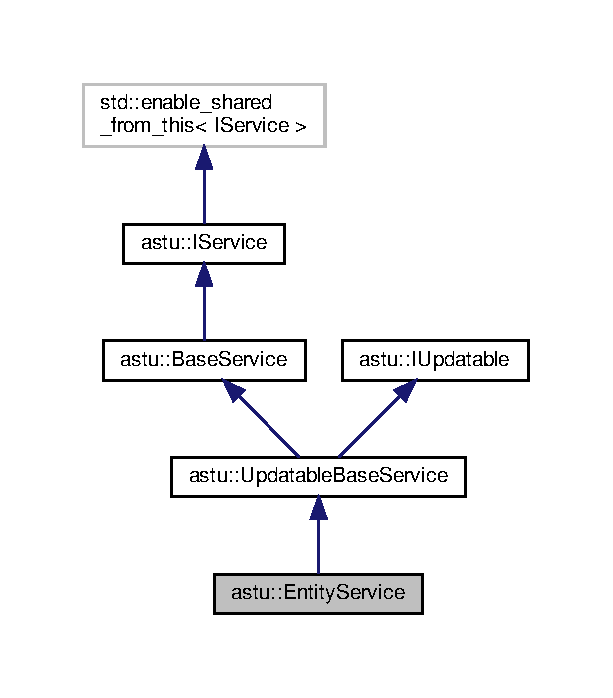
\includegraphics[width=262pt]{classastu_1_1EntityService__inherit__graph}
\end{center}
\end{figure}


Collaboration diagram for astu\+:\+:Entity\+Service\+:\nopagebreak
\begin{figure}[H]
\begin{center}
\leavevmode
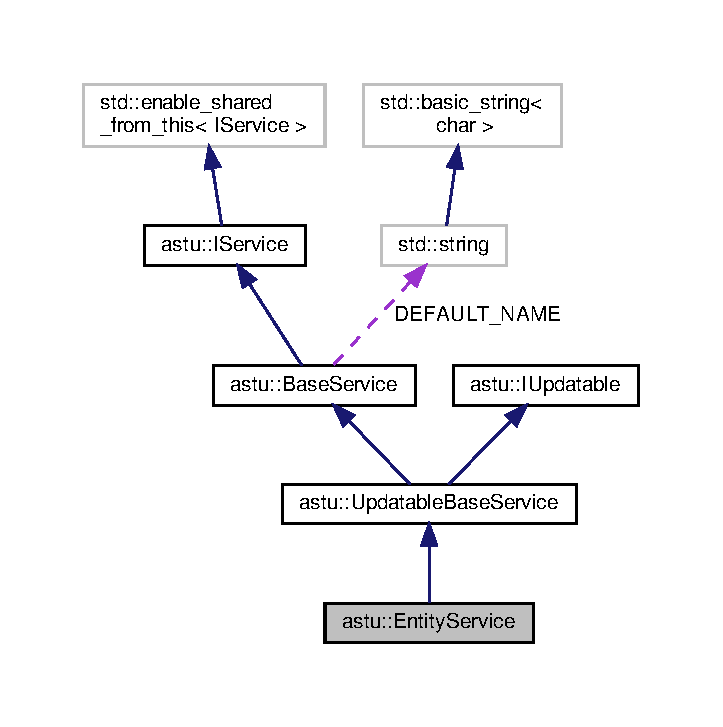
\includegraphics[width=309pt]{classastu_1_1EntityService__coll__graph}
\end{center}
\end{figure}
\subsection*{Public Member Functions}
\begin{DoxyCompactItemize}
\item 
\hyperlink{classastu_1_1EntityService_a74fc8d1e8b7aadf0899142c248cb2211}{Entity\+Service} (int update\+Priority=Priority\+::\+Normal)
\item 
void \hyperlink{classastu_1_1EntityService_ad6c6cb81dc8c48c7688f438571ee5da8}{Add\+Entity} (std\+::shared\+\_\+ptr$<$ \hyperlink{classastu_1_1Entity}{Entity} $>$ entity)
\item 
void \hyperlink{classastu_1_1EntityService_a748a71e470d5bb51bb650b15e0a78c63}{Remove\+Entity} (std\+::shared\+\_\+ptr$<$ \hyperlink{classastu_1_1Entity}{Entity} $>$ entity)
\item 
bool \hyperlink{classastu_1_1EntityService_a4a3c14fd7aa8edf4263913046744f277}{Has\+Entity} (std\+::shared\+\_\+ptr$<$ \hyperlink{classastu_1_1Entity}{Entity} $>$ entity) const
\item 
void \hyperlink{classastu_1_1EntityService_ac543fe51a3d1c9784bcab5775f5d388d}{Remove\+Entity} (\hyperlink{classastu_1_1Entity}{Entity} \&entity)
\item 
void \hyperlink{classastu_1_1EntityService_a1b21cf207324748c13c34568d3c1513e}{Remove\+All} ()
\item 
const std\+::shared\+\_\+ptr$<$ \hyperlink{group__ecs__group_gace2fb790b86c3908a65e4222f7ac2f4e}{Entity\+View} $>$ \hyperlink{classastu_1_1EntityService_aa295c07eb6a5c5321cf5820c9e41d008}{Get\+Entity\+View} (const \hyperlink{classastu_1_1EntityFamily}{Entity\+Family} \&family)
\item 
bool \hyperlink{classastu_1_1EntityService_a57fa7f62f90b8ecf4513045d7be9f15c}{Has\+Entity\+Listener} (const \hyperlink{classastu_1_1EntityFamily}{Entity\+Family} \&family, \hyperlink{classastu_1_1IEntityListener}{I\+Entity\+Listener} \&listener) const
\item 
void \hyperlink{classastu_1_1EntityService_ab338b1904b61dfe71c2b3bbcb390ada1}{Add\+Entity\+Listener} (const \hyperlink{classastu_1_1EntityFamily}{Entity\+Family} \&family, \hyperlink{classastu_1_1IEntityListener}{I\+Entity\+Listener} \&listener)
\item 
void \hyperlink{classastu_1_1EntityService_af9b12ecd243f0b0f98799fa2d147fecb}{Remove\+Entity\+Listener} (const \hyperlink{classastu_1_1EntityFamily}{Entity\+Family} \&family, \hyperlink{classastu_1_1IEntityListener}{I\+Entity\+Listener} \&listener)
\end{DoxyCompactItemize}
\subsection*{Protected Member Functions}
\begin{DoxyCompactItemize}
\item 
virtual void \hyperlink{classastu_1_1EntityService_a293ff7c8b84837b08cdabe98ed8a23ea}{On\+Startup} () override
\item 
virtual void \hyperlink{classastu_1_1EntityService_ac998c4d02a90460a129c8f2e0586d728}{On\+Shutdown} () override
\item 
virtual void \hyperlink{classastu_1_1EntityService_a70831a8dc185652c2c9056c4e3cc10e0}{On\+Update} () override
\end{DoxyCompactItemize}
\subsection*{Additional Inherited Members}


\subsection{Detailed Description}
The core service of the E\+CS, manages entities and entity listeners. 

\subsection{Constructor \& Destructor Documentation}
\mbox{\Hypertarget{classastu_1_1EntityService_a74fc8d1e8b7aadf0899142c248cb2211}\label{classastu_1_1EntityService_a74fc8d1e8b7aadf0899142c248cb2211}} 
\index{astu\+::\+Entity\+Service@{astu\+::\+Entity\+Service}!Entity\+Service@{Entity\+Service}}
\index{Entity\+Service@{Entity\+Service}!astu\+::\+Entity\+Service@{astu\+::\+Entity\+Service}}
\subsubsection{\texorpdfstring{Entity\+Service()}{EntityService()}}
{\footnotesize\ttfamily astu\+::\+Entity\+Service\+::\+Entity\+Service (\begin{DoxyParamCaption}\item[{int}]{update\+Priority = {\ttfamily Priority\+:\+:Normal} }\end{DoxyParamCaption})}

Constructor.


\begin{DoxyParams}{Parameters}
{\em update\+Priority} & the update priority of this service \\
\hline
\end{DoxyParams}


\subsection{Member Function Documentation}
\mbox{\Hypertarget{classastu_1_1EntityService_ad6c6cb81dc8c48c7688f438571ee5da8}\label{classastu_1_1EntityService_ad6c6cb81dc8c48c7688f438571ee5da8}} 
\index{astu\+::\+Entity\+Service@{astu\+::\+Entity\+Service}!Add\+Entity@{Add\+Entity}}
\index{Add\+Entity@{Add\+Entity}!astu\+::\+Entity\+Service@{astu\+::\+Entity\+Service}}
\subsubsection{\texorpdfstring{Add\+Entity()}{AddEntity()}}
{\footnotesize\ttfamily void astu\+::\+Entity\+Service\+::\+Add\+Entity (\begin{DoxyParamCaption}\item[{std\+::shared\+\_\+ptr$<$ \hyperlink{classastu_1_1Entity}{Entity} $>$}]{entity }\end{DoxyParamCaption})}

Adds an entity to this service.


\begin{DoxyParams}{Parameters}
{\em entity} & the entity to add \\
\hline
\end{DoxyParams}
\mbox{\Hypertarget{classastu_1_1EntityService_ab338b1904b61dfe71c2b3bbcb390ada1}\label{classastu_1_1EntityService_ab338b1904b61dfe71c2b3bbcb390ada1}} 
\index{astu\+::\+Entity\+Service@{astu\+::\+Entity\+Service}!Add\+Entity\+Listener@{Add\+Entity\+Listener}}
\index{Add\+Entity\+Listener@{Add\+Entity\+Listener}!astu\+::\+Entity\+Service@{astu\+::\+Entity\+Service}}
\subsubsection{\texorpdfstring{Add\+Entity\+Listener()}{AddEntityListener()}}
{\footnotesize\ttfamily void astu\+::\+Entity\+Service\+::\+Add\+Entity\+Listener (\begin{DoxyParamCaption}\item[{const \hyperlink{classastu_1_1EntityFamily}{Entity\+Family} \&}]{family,  }\item[{\hyperlink{classastu_1_1IEntityListener}{I\+Entity\+Listener} \&}]{listener }\end{DoxyParamCaption})}

Adds an entity listener to this service.


\begin{DoxyParams}{Parameters}
{\em family} & the entity family the listener is interested in \\
\hline
{\em listener} & the entity listener to add \\
\hline
\end{DoxyParams}
\mbox{\Hypertarget{classastu_1_1EntityService_aa295c07eb6a5c5321cf5820c9e41d008}\label{classastu_1_1EntityService_aa295c07eb6a5c5321cf5820c9e41d008}} 
\index{astu\+::\+Entity\+Service@{astu\+::\+Entity\+Service}!Get\+Entity\+View@{Get\+Entity\+View}}
\index{Get\+Entity\+View@{Get\+Entity\+View}!astu\+::\+Entity\+Service@{astu\+::\+Entity\+Service}}
\subsubsection{\texorpdfstring{Get\+Entity\+View()}{GetEntityView()}}
{\footnotesize\ttfamily const std\+::shared\+\_\+ptr$<$\hyperlink{group__ecs__group_gace2fb790b86c3908a65e4222f7ac2f4e}{Entity\+View}$>$ astu\+::\+Entity\+Service\+::\+Get\+Entity\+View (\begin{DoxyParamCaption}\item[{const \hyperlink{classastu_1_1EntityFamily}{Entity\+Family} \&}]{family }\end{DoxyParamCaption})}

Returns a view to a certain family of entities.

Any caller of this method can keep the returned pointer to the entity view. The view gets updated automatically when entities are added or removed.

\begin{DoxyReturn}{Returns}
the entity view 
\end{DoxyReturn}
\mbox{\Hypertarget{classastu_1_1EntityService_a4a3c14fd7aa8edf4263913046744f277}\label{classastu_1_1EntityService_a4a3c14fd7aa8edf4263913046744f277}} 
\index{astu\+::\+Entity\+Service@{astu\+::\+Entity\+Service}!Has\+Entity@{Has\+Entity}}
\index{Has\+Entity@{Has\+Entity}!astu\+::\+Entity\+Service@{astu\+::\+Entity\+Service}}
\subsubsection{\texorpdfstring{Has\+Entity()}{HasEntity()}}
{\footnotesize\ttfamily bool astu\+::\+Entity\+Service\+::\+Has\+Entity (\begin{DoxyParamCaption}\item[{std\+::shared\+\_\+ptr$<$ \hyperlink{classastu_1_1Entity}{Entity} $>$}]{entity }\end{DoxyParamCaption}) const}

Tests whether the specified entity exists.

\begin{DoxyReturn}{Returns}
{\ttfamily true} if the entity exists 
\end{DoxyReturn}
\mbox{\Hypertarget{classastu_1_1EntityService_a57fa7f62f90b8ecf4513045d7be9f15c}\label{classastu_1_1EntityService_a57fa7f62f90b8ecf4513045d7be9f15c}} 
\index{astu\+::\+Entity\+Service@{astu\+::\+Entity\+Service}!Has\+Entity\+Listener@{Has\+Entity\+Listener}}
\index{Has\+Entity\+Listener@{Has\+Entity\+Listener}!astu\+::\+Entity\+Service@{astu\+::\+Entity\+Service}}
\subsubsection{\texorpdfstring{Has\+Entity\+Listener()}{HasEntityListener()}}
{\footnotesize\ttfamily bool astu\+::\+Entity\+Service\+::\+Has\+Entity\+Listener (\begin{DoxyParamCaption}\item[{const \hyperlink{classastu_1_1EntityFamily}{Entity\+Family} \&}]{family,  }\item[{\hyperlink{classastu_1_1IEntityListener}{I\+Entity\+Listener} \&}]{listener }\end{DoxyParamCaption}) const}

Tests whether an entity listener has already been added.


\begin{DoxyParams}{Parameters}
{\em family} & the entity family the listener is interested in \\
\hline
{\em listener} & the entity listener to test \\
\hline
\end{DoxyParams}
\mbox{\Hypertarget{classastu_1_1EntityService_ac998c4d02a90460a129c8f2e0586d728}\label{classastu_1_1EntityService_ac998c4d02a90460a129c8f2e0586d728}} 
\index{astu\+::\+Entity\+Service@{astu\+::\+Entity\+Service}!On\+Shutdown@{On\+Shutdown}}
\index{On\+Shutdown@{On\+Shutdown}!astu\+::\+Entity\+Service@{astu\+::\+Entity\+Service}}
\subsubsection{\texorpdfstring{On\+Shutdown()}{OnShutdown()}}
{\footnotesize\ttfamily virtual void astu\+::\+Entity\+Service\+::\+On\+Shutdown (\begin{DoxyParamCaption}{ }\end{DoxyParamCaption})\hspace{0.3cm}{\ttfamily [override]}, {\ttfamily [protected]}, {\ttfamily [virtual]}}

Called by the service base method on shutdown.

Derived can override this method for de-\/initialization purposes, e.\+g., releasing resources, etc. 

Reimplemented from \hyperlink{classastu_1_1Service_a1e1dff727df791c57fae782d8a613c5f}{astu\+::\+Service}.

\mbox{\Hypertarget{classastu_1_1EntityService_a293ff7c8b84837b08cdabe98ed8a23ea}\label{classastu_1_1EntityService_a293ff7c8b84837b08cdabe98ed8a23ea}} 
\index{astu\+::\+Entity\+Service@{astu\+::\+Entity\+Service}!On\+Startup@{On\+Startup}}
\index{On\+Startup@{On\+Startup}!astu\+::\+Entity\+Service@{astu\+::\+Entity\+Service}}
\subsubsection{\texorpdfstring{On\+Startup()}{OnStartup()}}
{\footnotesize\ttfamily virtual void astu\+::\+Entity\+Service\+::\+On\+Startup (\begin{DoxyParamCaption}{ }\end{DoxyParamCaption})\hspace{0.3cm}{\ttfamily [override]}, {\ttfamily [protected]}, {\ttfamily [virtual]}}

Called by the service base class on startup.

Derived can override this method for initialization purposes. 

Reimplemented from \hyperlink{classastu_1_1Service_a357dc663e000b1f086f681ec3c459bfe}{astu\+::\+Service}.

\mbox{\Hypertarget{classastu_1_1EntityService_a70831a8dc185652c2c9056c4e3cc10e0}\label{classastu_1_1EntityService_a70831a8dc185652c2c9056c4e3cc10e0}} 
\index{astu\+::\+Entity\+Service@{astu\+::\+Entity\+Service}!On\+Update@{On\+Update}}
\index{On\+Update@{On\+Update}!astu\+::\+Entity\+Service@{astu\+::\+Entity\+Service}}
\subsubsection{\texorpdfstring{On\+Update()}{OnUpdate()}}
{\footnotesize\ttfamily virtual void astu\+::\+Entity\+Service\+::\+On\+Update (\begin{DoxyParamCaption}{ }\end{DoxyParamCaption})\hspace{0.3cm}{\ttfamily [override]}, {\ttfamily [protected]}, {\ttfamily [virtual]}}

Called when an update is due. 

Reimplemented from \hyperlink{classastu_1_1Updatable_a925566c9770b95895c6c7294f9d51528}{astu\+::\+Updatable}.

\mbox{\Hypertarget{classastu_1_1EntityService_a1b21cf207324748c13c34568d3c1513e}\label{classastu_1_1EntityService_a1b21cf207324748c13c34568d3c1513e}} 
\index{astu\+::\+Entity\+Service@{astu\+::\+Entity\+Service}!Remove\+All@{Remove\+All}}
\index{Remove\+All@{Remove\+All}!astu\+::\+Entity\+Service@{astu\+::\+Entity\+Service}}
\subsubsection{\texorpdfstring{Remove\+All()}{RemoveAll()}}
{\footnotesize\ttfamily void astu\+::\+Entity\+Service\+::\+Remove\+All (\begin{DoxyParamCaption}{ }\end{DoxyParamCaption})}

Removes all entities. \mbox{\Hypertarget{classastu_1_1EntityService_a748a71e470d5bb51bb650b15e0a78c63}\label{classastu_1_1EntityService_a748a71e470d5bb51bb650b15e0a78c63}} 
\index{astu\+::\+Entity\+Service@{astu\+::\+Entity\+Service}!Remove\+Entity@{Remove\+Entity}}
\index{Remove\+Entity@{Remove\+Entity}!astu\+::\+Entity\+Service@{astu\+::\+Entity\+Service}}
\subsubsection{\texorpdfstring{Remove\+Entity()}{RemoveEntity()}\hspace{0.1cm}{\footnotesize\ttfamily [1/2]}}
{\footnotesize\ttfamily void astu\+::\+Entity\+Service\+::\+Remove\+Entity (\begin{DoxyParamCaption}\item[{std\+::shared\+\_\+ptr$<$ \hyperlink{classastu_1_1Entity}{Entity} $>$}]{entity }\end{DoxyParamCaption})}

Removes an entity from this service.


\begin{DoxyParams}{Parameters}
{\em entity} & the entity to remove \\
\hline
\end{DoxyParams}
\mbox{\Hypertarget{classastu_1_1EntityService_ac543fe51a3d1c9784bcab5775f5d388d}\label{classastu_1_1EntityService_ac543fe51a3d1c9784bcab5775f5d388d}} 
\index{astu\+::\+Entity\+Service@{astu\+::\+Entity\+Service}!Remove\+Entity@{Remove\+Entity}}
\index{Remove\+Entity@{Remove\+Entity}!astu\+::\+Entity\+Service@{astu\+::\+Entity\+Service}}
\subsubsection{\texorpdfstring{Remove\+Entity()}{RemoveEntity()}\hspace{0.1cm}{\footnotesize\ttfamily [2/2]}}
{\footnotesize\ttfamily void astu\+::\+Entity\+Service\+::\+Remove\+Entity (\begin{DoxyParamCaption}\item[{\hyperlink{classastu_1_1Entity}{Entity} \&}]{entity }\end{DoxyParamCaption})\hspace{0.3cm}{\ttfamily [inline]}}

Removes an entity from this service.


\begin{DoxyParams}{Parameters}
{\em entity} & the entity to remove \\
\hline
\end{DoxyParams}
\mbox{\Hypertarget{classastu_1_1EntityService_af9b12ecd243f0b0f98799fa2d147fecb}\label{classastu_1_1EntityService_af9b12ecd243f0b0f98799fa2d147fecb}} 
\index{astu\+::\+Entity\+Service@{astu\+::\+Entity\+Service}!Remove\+Entity\+Listener@{Remove\+Entity\+Listener}}
\index{Remove\+Entity\+Listener@{Remove\+Entity\+Listener}!astu\+::\+Entity\+Service@{astu\+::\+Entity\+Service}}
\subsubsection{\texorpdfstring{Remove\+Entity\+Listener()}{RemoveEntityListener()}}
{\footnotesize\ttfamily void astu\+::\+Entity\+Service\+::\+Remove\+Entity\+Listener (\begin{DoxyParamCaption}\item[{const \hyperlink{classastu_1_1EntityFamily}{Entity\+Family} \&}]{family,  }\item[{\hyperlink{classastu_1_1IEntityListener}{I\+Entity\+Listener} \&}]{listener }\end{DoxyParamCaption})}

Removes an entity listener to from service.


\begin{DoxyParams}{Parameters}
{\em family} & the entity family the listener is interested in \\
\hline
{\em listener} & the entity listener to remove \\
\hline
\end{DoxyParams}


The documentation for this class was generated from the following file\+:\begin{DoxyCompactItemize}
\item 
include/\+E\+C\+S/Entity\+Service.\+h\end{DoxyCompactItemize}

\hypertarget{classastu_1_1IEntityListener}{}\section{astu\+:\+:I\+Entity\+Listener Class Reference}
\label{classastu_1_1IEntityListener}\index{astu\+::\+I\+Entity\+Listener@{astu\+::\+I\+Entity\+Listener}}


{\ttfamily \#include $<$Entity\+Service.\+h$>$}



Inheritance diagram for astu\+:\+:I\+Entity\+Listener\+:\nopagebreak
\begin{figure}[H]
\begin{center}
\leavevmode
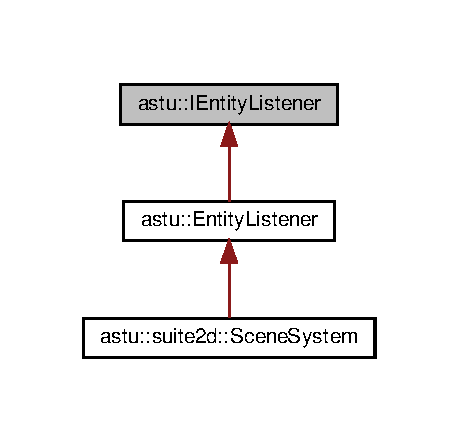
\includegraphics[width=220pt]{classastu_1_1IEntityListener__inherit__graph}
\end{center}
\end{figure}
\subsection*{Public Member Functions}
\begin{DoxyCompactItemize}
\item 
virtual \hyperlink{classastu_1_1IEntityListener_ad3e01cd267ff128c2176d06897c8c7b6}{$\sim$\+I\+Entity\+Listener} ()
\item 
virtual void \hyperlink{classastu_1_1IEntityListener_afa087302fdf0bd999297b0d35ceb1f61}{On\+Entity\+Added} (std\+::shared\+\_\+ptr$<$ \hyperlink{classastu_1_1Entity}{astu\+::\+Entity} $>$ entity)=0
\item 
virtual void \hyperlink{classastu_1_1IEntityListener_ab3d5a276da5e42cc4831e747fdf11718}{On\+Entity\+Removed} (std\+::shared\+\_\+ptr$<$ \hyperlink{classastu_1_1Entity}{astu\+::\+Entity} $>$ entity)=0
\end{DoxyCompactItemize}


\subsection{Detailed Description}
Interface for entity listeners which get informed when entities get added or removed. 

\subsection{Constructor \& Destructor Documentation}
\mbox{\Hypertarget{classastu_1_1IEntityListener_ad3e01cd267ff128c2176d06897c8c7b6}\label{classastu_1_1IEntityListener_ad3e01cd267ff128c2176d06897c8c7b6}} 
\index{astu\+::\+I\+Entity\+Listener@{astu\+::\+I\+Entity\+Listener}!````~I\+Entity\+Listener@{$\sim$\+I\+Entity\+Listener}}
\index{````~I\+Entity\+Listener@{$\sim$\+I\+Entity\+Listener}!astu\+::\+I\+Entity\+Listener@{astu\+::\+I\+Entity\+Listener}}
\subsubsection{\texorpdfstring{$\sim$\+I\+Entity\+Listener()}{~IEntityListener()}}
{\footnotesize\ttfamily virtual astu\+::\+I\+Entity\+Listener\+::$\sim$\+I\+Entity\+Listener (\begin{DoxyParamCaption}{ }\end{DoxyParamCaption})\hspace{0.3cm}{\ttfamily [inline]}, {\ttfamily [virtual]}}

Virtual destructor. 

\subsection{Member Function Documentation}
\mbox{\Hypertarget{classastu_1_1IEntityListener_afa087302fdf0bd999297b0d35ceb1f61}\label{classastu_1_1IEntityListener_afa087302fdf0bd999297b0d35ceb1f61}} 
\index{astu\+::\+I\+Entity\+Listener@{astu\+::\+I\+Entity\+Listener}!On\+Entity\+Added@{On\+Entity\+Added}}
\index{On\+Entity\+Added@{On\+Entity\+Added}!astu\+::\+I\+Entity\+Listener@{astu\+::\+I\+Entity\+Listener}}
\subsubsection{\texorpdfstring{On\+Entity\+Added()}{OnEntityAdded()}}
{\footnotesize\ttfamily virtual void astu\+::\+I\+Entity\+Listener\+::\+On\+Entity\+Added (\begin{DoxyParamCaption}\item[{std\+::shared\+\_\+ptr$<$ \hyperlink{classastu_1_1Entity}{astu\+::\+Entity} $>$}]{entity }\end{DoxyParamCaption})\hspace{0.3cm}{\ttfamily [pure virtual]}}

Called when an entity has been added.


\begin{DoxyParams}{Parameters}
{\em entity} & the entity which has been added \\
\hline
\end{DoxyParams}


Implemented in \hyperlink{classastu_1_1EntityListener_a0c123b57dcabc4c2b6cee8f05db545c8}{astu\+::\+Entity\+Listener}.

\mbox{\Hypertarget{classastu_1_1IEntityListener_ab3d5a276da5e42cc4831e747fdf11718}\label{classastu_1_1IEntityListener_ab3d5a276da5e42cc4831e747fdf11718}} 
\index{astu\+::\+I\+Entity\+Listener@{astu\+::\+I\+Entity\+Listener}!On\+Entity\+Removed@{On\+Entity\+Removed}}
\index{On\+Entity\+Removed@{On\+Entity\+Removed}!astu\+::\+I\+Entity\+Listener@{astu\+::\+I\+Entity\+Listener}}
\subsubsection{\texorpdfstring{On\+Entity\+Removed()}{OnEntityRemoved()}}
{\footnotesize\ttfamily virtual void astu\+::\+I\+Entity\+Listener\+::\+On\+Entity\+Removed (\begin{DoxyParamCaption}\item[{std\+::shared\+\_\+ptr$<$ \hyperlink{classastu_1_1Entity}{astu\+::\+Entity} $>$}]{entity }\end{DoxyParamCaption})\hspace{0.3cm}{\ttfamily [pure virtual]}}

Called when an entity has been removed.


\begin{DoxyParams}{Parameters}
{\em entity} & the entity which has been removed \\
\hline
\end{DoxyParams}


Implemented in \hyperlink{classastu_1_1EntityListener_ae380d941fafd6933a9f290ac50e7f32b}{astu\+::\+Entity\+Listener}.



The documentation for this class was generated from the following file\+:\begin{DoxyCompactItemize}
\item 
include/\+E\+C\+S/Entity\+Service.\+h\end{DoxyCompactItemize}

\hypertarget{classastu_1_1Image}{}\section{astu\+:\+:Image Class Reference}
\label{classastu_1_1Image}\index{astu\+::\+Image@{astu\+::\+Image}}


{\ttfamily \#include $<$Image.\+h$>$}

\subsection*{Public Member Functions}
\begin{DoxyCompactItemize}
\item 
\hyperlink{classastu_1_1Image_a930c3dfe86d60d209199cf27d2102446}{Image} (int w, int h)
\item 
int \hyperlink{classastu_1_1Image_a654888b88e109da1099ade3ec54f0520}{Get\+Width} () const
\item 
int \hyperlink{classastu_1_1Image_ad64d3b2abc18e54ba8beb4e212a75a10}{Get\+Height} () const
\item 
double \hyperlink{classastu_1_1Image_a06bdd931e5090f1eca62bd305b83cfd5}{Get\+Aspect\+Ratio} () const
\item 
const \hyperlink{classastu_1_1Color}{Color} \& \hyperlink{classastu_1_1Image_a8a31850315f2c74bc90627f4a292a10d}{Get\+Pixel} (int x, int y) const
\item 
void \hyperlink{classastu_1_1Image_a3c4770367d30abf8cefaa5cf777501a4}{Set\+Pixel} (int x, int y, const \hyperlink{classastu_1_1Color}{Color} \&c)
\item 
const \hyperlink{classastu_1_1Color}{Color} \& \hyperlink{classastu_1_1Image_a0ff83b1620356fdbe3ee3771d8a3ddb2}{Get\+Pixel} (size\+\_\+t idx) const
\item 
void \hyperlink{classastu_1_1Image_a1c2f1673fbba03abc50101c2d75ef12e}{Set\+Pixel} (size\+\_\+t idx, const \hyperlink{classastu_1_1Color}{Color} \&c)
\item 
size\+\_\+t \hyperlink{classastu_1_1Image_a53c53ecc0210786efa7f514966ad406b}{Number\+Of\+Pixels} () const
\item 
\hyperlink{classastu_1_1Color}{Color} $\ast$ \hyperlink{classastu_1_1Image_a3ce797d40010a7536662562c5f2e52da}{Get\+Pixels} ()
\item 
const \hyperlink{classastu_1_1Color}{Color} $\ast$ \hyperlink{classastu_1_1Image_ad2f3de6cc397bbc924c3718e54b1182f}{Get\+Pixels} () const
\end{DoxyCompactItemize}


\subsection{Detailed Description}
This class represents an image where each individual pixel is represented as instances of the class \hyperlink{classastu_1_1Color}{Color}. The \hyperlink{classastu_1_1Color}{Color} class represents a pixel as R\+G\+BA (red, green, blue and alpha channel) floating-\/point components.

Representing an image this way offers a convenient and straightforward way and maintains high color precision. However, memory consumption and performance might suffer. This class is preferably used for image synthesis and analysis. 

\subsection{Constructor \& Destructor Documentation}
\mbox{\Hypertarget{classastu_1_1Image_a930c3dfe86d60d209199cf27d2102446}\label{classastu_1_1Image_a930c3dfe86d60d209199cf27d2102446}} 
\index{astu\+::\+Image@{astu\+::\+Image}!Image@{Image}}
\index{Image@{Image}!astu\+::\+Image@{astu\+::\+Image}}
\subsubsection{\texorpdfstring{Image()}{Image()}}
{\footnotesize\ttfamily astu\+::\+Image\+::\+Image (\begin{DoxyParamCaption}\item[{int}]{w,  }\item[{int}]{h }\end{DoxyParamCaption})}

Constructor.


\begin{DoxyParams}{Parameters}
{\em w} & the width of the image in pixels \\
\hline
{\em h} & the height of the image in pixels \\
\hline
\end{DoxyParams}

\begin{DoxyExceptions}{Exceptions}
{\em std\+::domain\+\_\+error} & in case the width or height is \\
\hline
\end{DoxyExceptions}


\subsection{Member Function Documentation}
\mbox{\Hypertarget{classastu_1_1Image_a06bdd931e5090f1eca62bd305b83cfd5}\label{classastu_1_1Image_a06bdd931e5090f1eca62bd305b83cfd5}} 
\index{astu\+::\+Image@{astu\+::\+Image}!Get\+Aspect\+Ratio@{Get\+Aspect\+Ratio}}
\index{Get\+Aspect\+Ratio@{Get\+Aspect\+Ratio}!astu\+::\+Image@{astu\+::\+Image}}
\subsubsection{\texorpdfstring{Get\+Aspect\+Ratio()}{GetAspectRatio()}}
{\footnotesize\ttfamily double astu\+::\+Image\+::\+Get\+Aspect\+Ratio (\begin{DoxyParamCaption}{ }\end{DoxyParamCaption}) const\hspace{0.3cm}{\ttfamily [inline]}}

Returns the aspect ratio of this image.

\begin{DoxyReturn}{Returns}
the aspect ratio 
\end{DoxyReturn}
\mbox{\Hypertarget{classastu_1_1Image_ad64d3b2abc18e54ba8beb4e212a75a10}\label{classastu_1_1Image_ad64d3b2abc18e54ba8beb4e212a75a10}} 
\index{astu\+::\+Image@{astu\+::\+Image}!Get\+Height@{Get\+Height}}
\index{Get\+Height@{Get\+Height}!astu\+::\+Image@{astu\+::\+Image}}
\subsubsection{\texorpdfstring{Get\+Height()}{GetHeight()}}
{\footnotesize\ttfamily int astu\+::\+Image\+::\+Get\+Height (\begin{DoxyParamCaption}{ }\end{DoxyParamCaption}) const\hspace{0.3cm}{\ttfamily [inline]}}

Returns the height of this image

\begin{DoxyReturn}{Returns}
the height of this image in pixel 
\end{DoxyReturn}
\mbox{\Hypertarget{classastu_1_1Image_a8a31850315f2c74bc90627f4a292a10d}\label{classastu_1_1Image_a8a31850315f2c74bc90627f4a292a10d}} 
\index{astu\+::\+Image@{astu\+::\+Image}!Get\+Pixel@{Get\+Pixel}}
\index{Get\+Pixel@{Get\+Pixel}!astu\+::\+Image@{astu\+::\+Image}}
\subsubsection{\texorpdfstring{Get\+Pixel()}{GetPixel()}\hspace{0.1cm}{\footnotesize\ttfamily [1/2]}}
{\footnotesize\ttfamily const \hyperlink{classastu_1_1Color}{Color}\& astu\+::\+Image\+::\+Get\+Pixel (\begin{DoxyParamCaption}\item[{int}]{x,  }\item[{int}]{y }\end{DoxyParamCaption}) const}

Returns the color of a pixel.


\begin{DoxyParams}{Parameters}
{\em x} & the x-\/coordinate of the pixel \\
\hline
{\em y} & the y-\/coordinate of the pixel \\
\hline
\end{DoxyParams}
\begin{DoxyReturn}{Returns}
the color at the specified location 
\end{DoxyReturn}

\begin{DoxyExceptions}{Exceptions}
{\em std\+::out\+\_\+of\+\_\+range} & in case the coordinates are invalid \\
\hline
\end{DoxyExceptions}
\mbox{\Hypertarget{classastu_1_1Image_a0ff83b1620356fdbe3ee3771d8a3ddb2}\label{classastu_1_1Image_a0ff83b1620356fdbe3ee3771d8a3ddb2}} 
\index{astu\+::\+Image@{astu\+::\+Image}!Get\+Pixel@{Get\+Pixel}}
\index{Get\+Pixel@{Get\+Pixel}!astu\+::\+Image@{astu\+::\+Image}}
\subsubsection{\texorpdfstring{Get\+Pixel()}{GetPixel()}\hspace{0.1cm}{\footnotesize\ttfamily [2/2]}}
{\footnotesize\ttfamily const \hyperlink{classastu_1_1Color}{Color}\& astu\+::\+Image\+::\+Get\+Pixel (\begin{DoxyParamCaption}\item[{size\+\_\+t}]{idx }\end{DoxyParamCaption}) const}

Returns the color of a pixel.


\begin{DoxyParams}{Parameters}
{\em idx} & the linear index of the pixel \\
\hline
\end{DoxyParams}
\begin{DoxyReturn}{Returns}
the color of the pixel at the specified location 
\end{DoxyReturn}

\begin{DoxyExceptions}{Exceptions}
{\em std\+::out\+\_\+of\+\_\+range} & in case the index is invalid \\
\hline
\end{DoxyExceptions}
\mbox{\Hypertarget{classastu_1_1Image_a3ce797d40010a7536662562c5f2e52da}\label{classastu_1_1Image_a3ce797d40010a7536662562c5f2e52da}} 
\index{astu\+::\+Image@{astu\+::\+Image}!Get\+Pixels@{Get\+Pixels}}
\index{Get\+Pixels@{Get\+Pixels}!astu\+::\+Image@{astu\+::\+Image}}
\subsubsection{\texorpdfstring{Get\+Pixels()}{GetPixels()}\hspace{0.1cm}{\footnotesize\ttfamily [1/2]}}
{\footnotesize\ttfamily \hyperlink{classastu_1_1Color}{Color}$\ast$ astu\+::\+Image\+::\+Get\+Pixels (\begin{DoxyParamCaption}{ }\end{DoxyParamCaption})}

This method provides raw access to the pixel colors, use with care.

\begin{DoxyReturn}{Returns}
pointer to the linear array of pixel colors 
\end{DoxyReturn}
\mbox{\Hypertarget{classastu_1_1Image_ad2f3de6cc397bbc924c3718e54b1182f}\label{classastu_1_1Image_ad2f3de6cc397bbc924c3718e54b1182f}} 
\index{astu\+::\+Image@{astu\+::\+Image}!Get\+Pixels@{Get\+Pixels}}
\index{Get\+Pixels@{Get\+Pixels}!astu\+::\+Image@{astu\+::\+Image}}
\subsubsection{\texorpdfstring{Get\+Pixels()}{GetPixels()}\hspace{0.1cm}{\footnotesize\ttfamily [2/2]}}
{\footnotesize\ttfamily const \hyperlink{classastu_1_1Color}{Color}$\ast$ astu\+::\+Image\+::\+Get\+Pixels (\begin{DoxyParamCaption}{ }\end{DoxyParamCaption}) const}

This method provides raw access to the pixel colors, use with care.

This version returns a const pointer to the array and does not allow the modify the color values.

\begin{DoxyReturn}{Returns}
pointer to the linear array of pixel colors 
\end{DoxyReturn}
\mbox{\Hypertarget{classastu_1_1Image_a654888b88e109da1099ade3ec54f0520}\label{classastu_1_1Image_a654888b88e109da1099ade3ec54f0520}} 
\index{astu\+::\+Image@{astu\+::\+Image}!Get\+Width@{Get\+Width}}
\index{Get\+Width@{Get\+Width}!astu\+::\+Image@{astu\+::\+Image}}
\subsubsection{\texorpdfstring{Get\+Width()}{GetWidth()}}
{\footnotesize\ttfamily int astu\+::\+Image\+::\+Get\+Width (\begin{DoxyParamCaption}{ }\end{DoxyParamCaption}) const\hspace{0.3cm}{\ttfamily [inline]}}

Returns the width of this image

\begin{DoxyReturn}{Returns}
the width of this image in pixel 
\end{DoxyReturn}
\mbox{\Hypertarget{classastu_1_1Image_a53c53ecc0210786efa7f514966ad406b}\label{classastu_1_1Image_a53c53ecc0210786efa7f514966ad406b}} 
\index{astu\+::\+Image@{astu\+::\+Image}!Number\+Of\+Pixels@{Number\+Of\+Pixels}}
\index{Number\+Of\+Pixels@{Number\+Of\+Pixels}!astu\+::\+Image@{astu\+::\+Image}}
\subsubsection{\texorpdfstring{Number\+Of\+Pixels()}{NumberOfPixels()}}
{\footnotesize\ttfamily size\+\_\+t astu\+::\+Image\+::\+Number\+Of\+Pixels (\begin{DoxyParamCaption}{ }\end{DoxyParamCaption}) const}

Returns the number of pixels of this image.

The number of pixels equals width times height of this image.

\begin{DoxyReturn}{Returns}
the number of pixels 
\end{DoxyReturn}
\mbox{\Hypertarget{classastu_1_1Image_a3c4770367d30abf8cefaa5cf777501a4}\label{classastu_1_1Image_a3c4770367d30abf8cefaa5cf777501a4}} 
\index{astu\+::\+Image@{astu\+::\+Image}!Set\+Pixel@{Set\+Pixel}}
\index{Set\+Pixel@{Set\+Pixel}!astu\+::\+Image@{astu\+::\+Image}}
\subsubsection{\texorpdfstring{Set\+Pixel()}{SetPixel()}\hspace{0.1cm}{\footnotesize\ttfamily [1/2]}}
{\footnotesize\ttfamily void astu\+::\+Image\+::\+Set\+Pixel (\begin{DoxyParamCaption}\item[{int}]{x,  }\item[{int}]{y,  }\item[{const \hyperlink{classastu_1_1Color}{Color} \&}]{c }\end{DoxyParamCaption})}

Sets the color of a pixel.


\begin{DoxyParams}{Parameters}
{\em x} & the x-\/coordinate of the pixel \\
\hline
{\em y} & the y-\/coordinate of the pixel \\
\hline
{\em c} & the new color \\
\hline
\end{DoxyParams}

\begin{DoxyExceptions}{Exceptions}
{\em std\+::out\+\_\+of\+\_\+range} & in case the coordinates are invalid \\
\hline
\end{DoxyExceptions}
\mbox{\Hypertarget{classastu_1_1Image_a1c2f1673fbba03abc50101c2d75ef12e}\label{classastu_1_1Image_a1c2f1673fbba03abc50101c2d75ef12e}} 
\index{astu\+::\+Image@{astu\+::\+Image}!Set\+Pixel@{Set\+Pixel}}
\index{Set\+Pixel@{Set\+Pixel}!astu\+::\+Image@{astu\+::\+Image}}
\subsubsection{\texorpdfstring{Set\+Pixel()}{SetPixel()}\hspace{0.1cm}{\footnotesize\ttfamily [2/2]}}
{\footnotesize\ttfamily void astu\+::\+Image\+::\+Set\+Pixel (\begin{DoxyParamCaption}\item[{size\+\_\+t}]{idx,  }\item[{const \hyperlink{classastu_1_1Color}{Color} \&}]{c }\end{DoxyParamCaption})}

Sets the color of a pixel.


\begin{DoxyParams}{Parameters}
{\em idx} & the linear index of the pixel \\
\hline
{\em c} & the new color of the pixel at the specified location \\
\hline
\end{DoxyParams}

\begin{DoxyExceptions}{Exceptions}
{\em std\+::out\+\_\+of\+\_\+range} & in case the index is invalid \\
\hline
\end{DoxyExceptions}


The documentation for this class was generated from the following file\+:\begin{DoxyCompactItemize}
\item 
include/Image.\+h\end{DoxyCompactItemize}

\hypertarget{classastu_1_1ImageRenderer}{}\section{astu\+:\+:Image\+Renderer Class Reference}
\label{classastu_1_1ImageRenderer}\index{astu\+::\+Image\+Renderer@{astu\+::\+Image\+Renderer}}


{\ttfamily \#include $<$Image\+Renderer.\+h$>$}

\subsection*{Public Member Functions}
\begin{DoxyCompactItemize}
\item 
\hyperlink{classastu_1_1ImageRenderer_a88dc5f8ff5aa6a039c1c77c31bd5bb89}{Image\+Renderer} ()
\item 
\hyperlink{classastu_1_1ImageRenderer_ac35d79e814253e2a2755da114e05d05c}{$\sim$\+Image\+Renderer} ()
\item 
void \hyperlink{classastu_1_1ImageRenderer_ae81b23f9e19254a7923cadf2a9e081a3}{Clear} ()
\item 
void \hyperlink{classastu_1_1ImageRenderer_a902cdac5634067b5e78de3f91667d1b9}{Set\+Draw\+Color} (const \hyperlink{classastu_1_1Color}{Color} \&c)
\item 
void \hyperlink{classastu_1_1ImageRenderer_acfb25962b67295325e9209759fcabe2b}{Set\+Background\+Color} (const \hyperlink{classastu_1_1Color}{Color} \&c)
\item 
void \hyperlink{classastu_1_1ImageRenderer_a903b1b78edee5f09b9ee1f604d762c28}{Draw\+Circle} (double cx, double cy, double r)
\item 
void \hyperlink{classastu_1_1ImageRenderer_a914047284fae6e8f58614018c8575f4e}{Draw\+Circle} (const Vector2$<$ double $>$ \&c, double r)
\item 
void \hyperlink{classastu_1_1ImageRenderer_a968b3ac1ef2611e149494d0855fbab85}{Draw\+Line} (const Vector2$<$ double $>$ \&p0, const Vector2$<$ double $>$ \&p1, double w=1)
\item 
void \hyperlink{classastu_1_1ImageRenderer_ae9e54c2f75cc76b9d45216df81b92aa4}{Draw\+Line} (double x0, double y0, double x1, double y1, double w=1)
\item 
void \hyperlink{classastu_1_1ImageRenderer_a95ed0bcec030e0ab17d0c6abc104eac3}{Draw\+Rectangle} (double cx, double cy, double w, double h, double angle\+Deg=0)
\item 
void \hyperlink{classastu_1_1ImageRenderer_a43f82202ac8ffdeba33fd5ecc600c267}{Draw\+Rectangle} (const Vector2$<$ double $>$ \&center, double w, double h, double angle\+Deg=0)
\item 
void \hyperlink{classastu_1_1ImageRenderer_a154491f8ef39881eeaba56f9d8ca24e8}{Set\+Render\+Quality} (\hyperlink{group__gfx__group_gac3b4955f341cea44f53f8446d734cd54}{Render\+Quality} quality)
\item 
\hyperlink{group__gfx__group_gac3b4955f341cea44f53f8446d734cd54}{Render\+Quality} \hyperlink{classastu_1_1ImageRenderer_a7f3f1cc8129dd8e40dea73e7f1333769}{Get\+Render\+Quality} () const
\item 
void \hyperlink{classastu_1_1ImageRenderer_a55172edcac396d7840da655697d57e28}{Render} (\hyperlink{classastu_1_1Image}{Image} \&img)
\end{DoxyCompactItemize}


\subsection{Detailed Description}
This class can be used to render geometric primitives in an resolution independent way. The output of the rendering will be an \hyperlink{classastu_1_1Image}{Image}.

{\bfseries Example Usage}


\begin{DoxyCode}
\textcolor{preprocessor}{#include <stdexcept>}
\textcolor{preprocessor}{#include <iostream>}
\textcolor{preprocessor}{#include <\hyperlink{AstGraphics_8h}{AstGraphics.h}>}

\textcolor{keyword}{using namespace }\hyperlink{namespacestd}{std};
\textcolor{keyword}{using namespace }\hyperlink{namespaceastu}{astu};

\textcolor{keywordtype}{int} main()
\{
  \textcolor{keyword}{const} \textcolor{keywordtype}{int} kWidth = 512;
  \textcolor{keyword}{const} \textcolor{keywordtype}{int} kHeight = 512;

  \hyperlink{classastu_1_1ImageRenderer}{ImageRenderer} renderer;

  \textcolor{comment}{// Create some graphical elements.}
  renderer.\hyperlink{classastu_1_1ImageRenderer_a902cdac5634067b5e78de3f91667d1b9}{SetDrawColor}(\hyperlink{classastu_1_1Color}{Color}(1.0, 0.8, 0.5, 0.5));
  renderer.\hyperlink{classastu_1_1ImageRenderer_a95ed0bcec030e0ab17d0c6abc104eac3}{DrawRectangle}(kWidth / 2.0, kHeight / 2.0, kHeight, 50);

  renderer.\hyperlink{classastu_1_1ImageRenderer_a902cdac5634067b5e78de3f91667d1b9}{SetDrawColor}(\hyperlink{group__gfx__group_gga6f6f9db1751e96b647084ecaedff2409a4f06dbd0c0981a97dd9279788b11a457}{WebColors::Red});
  renderer.\hyperlink{classastu_1_1ImageRenderer_a903b1b78edee5f09b9ee1f604d762c28}{DrawCircle}(kWidth / 2.0, kHeight / 2.0, 100.0);

  renderer.\hyperlink{classastu_1_1ImageRenderer_a902cdac5634067b5e78de3f91667d1b9}{SetDrawColor}(\hyperlink{classastu_1_1Color}{Color}(1.0, 0.8, 0.5, 0.5));
  renderer.\hyperlink{classastu_1_1ImageRenderer_a95ed0bcec030e0ab17d0c6abc104eac3}{DrawRectangle}(kWidth / 2.0, kHeight / 2.0, 50, kWidth);

  renderer.\hyperlink{classastu_1_1ImageRenderer_a902cdac5634067b5e78de3f91667d1b9}{SetDrawColor}(\hyperlink{group__gfx__group_gga6f6f9db1751e96b647084ecaedff2409a384d49f1ac85f826658bccf8f6c778f9}{WebColors::Green});
  renderer.\hyperlink{classastu_1_1ImageRenderer_a95ed0bcec030e0ab17d0c6abc104eac3}{DrawRectangle}(kWidth / 4.0, kHeight / 4.0, 50, 50, 45);

  \textcolor{comment}{// Background can be defined at any time.}
  renderer.\hyperlink{classastu_1_1ImageRenderer_acfb25962b67295325e9209759fcabe2b}{SetBackgroundColor}(\hyperlink{group__gfx__group_gga6f6f9db1751e96b647084ecaedff2409ae2e0a544fd90f604852d4c9564d64b36}{WebColors::White});


  \textcolor{comment}{// Render Image }
  \hyperlink{classastu_1_1Image}{Image} image(kWidth, kHeight);
  renderer.\hyperlink{classastu_1_1ImageRenderer_a154491f8ef39881eeaba56f9d8ca24e8}{SetRenderQuality}(\hyperlink{group__gfx__group_ggac3b4955f341cea44f53f8446d734cd54a0c6ad70beb3a7e76c3fc7adab7c46acc}{RenderQuality::Good});
  std::cout << \textcolor{stringliteral}{"Rendering image"} << std::endl;
  renderer.\hyperlink{classastu_1_1ImageRenderer_a55172edcac396d7840da655697d57e28}{Render}(image);

  \textcolor{comment}{// Store image to file, might cause an exception in case}
  \textcolor{comment}{// of an I/O error.}
  \textcolor{keywordflow}{try} \{
    \hyperlink{group__gfx__group_gaca5f9cb8047c60049300242c20d30cd6}{StoreImage}(image, \textcolor{stringliteral}{"output.bmp"});
  \} \textcolor{keywordflow}{catch} (std::runtime\_error & e) \{
    std::cout << \textcolor{stringliteral}{"Error storing image: "} << e.what() << std::endl;
    \textcolor{keywordflow}{return} -1;
  \}

  \textcolor{keywordflow}{return} 0;
\}     
\end{DoxyCode}


This code will generate this image\+:

 

\subsection{Constructor \& Destructor Documentation}
\mbox{\Hypertarget{classastu_1_1ImageRenderer_a88dc5f8ff5aa6a039c1c77c31bd5bb89}\label{classastu_1_1ImageRenderer_a88dc5f8ff5aa6a039c1c77c31bd5bb89}} 
\index{astu\+::\+Image\+Renderer@{astu\+::\+Image\+Renderer}!Image\+Renderer@{Image\+Renderer}}
\index{Image\+Renderer@{Image\+Renderer}!astu\+::\+Image\+Renderer@{astu\+::\+Image\+Renderer}}
\subsubsection{\texorpdfstring{Image\+Renderer()}{ImageRenderer()}}
{\footnotesize\ttfamily astu\+::\+Image\+Renderer\+::\+Image\+Renderer (\begin{DoxyParamCaption}{ }\end{DoxyParamCaption})}

Constructor. \mbox{\Hypertarget{classastu_1_1ImageRenderer_ac35d79e814253e2a2755da114e05d05c}\label{classastu_1_1ImageRenderer_ac35d79e814253e2a2755da114e05d05c}} 
\index{astu\+::\+Image\+Renderer@{astu\+::\+Image\+Renderer}!````~Image\+Renderer@{$\sim$\+Image\+Renderer}}
\index{````~Image\+Renderer@{$\sim$\+Image\+Renderer}!astu\+::\+Image\+Renderer@{astu\+::\+Image\+Renderer}}
\subsubsection{\texorpdfstring{$\sim$\+Image\+Renderer()}{~ImageRenderer()}}
{\footnotesize\ttfamily astu\+::\+Image\+Renderer\+::$\sim$\+Image\+Renderer (\begin{DoxyParamCaption}{ }\end{DoxyParamCaption})}

Destructor. 

\subsection{Member Function Documentation}
\mbox{\Hypertarget{classastu_1_1ImageRenderer_ae81b23f9e19254a7923cadf2a9e081a3}\label{classastu_1_1ImageRenderer_ae81b23f9e19254a7923cadf2a9e081a3}} 
\index{astu\+::\+Image\+Renderer@{astu\+::\+Image\+Renderer}!Clear@{Clear}}
\index{Clear@{Clear}!astu\+::\+Image\+Renderer@{astu\+::\+Image\+Renderer}}
\subsubsection{\texorpdfstring{Clear()}{Clear()}}
{\footnotesize\ttfamily void astu\+::\+Image\+Renderer\+::\+Clear (\begin{DoxyParamCaption}{ }\end{DoxyParamCaption})}

Clear the output rendering. \mbox{\Hypertarget{classastu_1_1ImageRenderer_a903b1b78edee5f09b9ee1f604d762c28}\label{classastu_1_1ImageRenderer_a903b1b78edee5f09b9ee1f604d762c28}} 
\index{astu\+::\+Image\+Renderer@{astu\+::\+Image\+Renderer}!Draw\+Circle@{Draw\+Circle}}
\index{Draw\+Circle@{Draw\+Circle}!astu\+::\+Image\+Renderer@{astu\+::\+Image\+Renderer}}
\subsubsection{\texorpdfstring{Draw\+Circle()}{DrawCircle()}\hspace{0.1cm}{\footnotesize\ttfamily [1/2]}}
{\footnotesize\ttfamily void astu\+::\+Image\+Renderer\+::\+Draw\+Circle (\begin{DoxyParamCaption}\item[{double}]{cx,  }\item[{double}]{cy,  }\item[{double}]{r }\end{DoxyParamCaption})}

Draws a filled circle.


\begin{DoxyParams}{Parameters}
{\em cx} & the x-\/coordinate of the center of the circle \\
\hline
{\em cy} & the y-\/coordinate of the center of the circle \\
\hline
{\em r} & the radius of the circle \\
\hline
\end{DoxyParams}
\mbox{\Hypertarget{classastu_1_1ImageRenderer_a914047284fae6e8f58614018c8575f4e}\label{classastu_1_1ImageRenderer_a914047284fae6e8f58614018c8575f4e}} 
\index{astu\+::\+Image\+Renderer@{astu\+::\+Image\+Renderer}!Draw\+Circle@{Draw\+Circle}}
\index{Draw\+Circle@{Draw\+Circle}!astu\+::\+Image\+Renderer@{astu\+::\+Image\+Renderer}}
\subsubsection{\texorpdfstring{Draw\+Circle()}{DrawCircle()}\hspace{0.1cm}{\footnotesize\ttfamily [2/2]}}
{\footnotesize\ttfamily void astu\+::\+Image\+Renderer\+::\+Draw\+Circle (\begin{DoxyParamCaption}\item[{const Vector2$<$ double $>$ \&}]{c,  }\item[{double}]{r }\end{DoxyParamCaption})\hspace{0.3cm}{\ttfamily [inline]}}

Draws a filled circle.


\begin{DoxyParams}{Parameters}
{\em c} & the center of the circle \\
\hline
{\em r} & the radius of the circle \\
\hline
\end{DoxyParams}
\mbox{\Hypertarget{classastu_1_1ImageRenderer_a968b3ac1ef2611e149494d0855fbab85}\label{classastu_1_1ImageRenderer_a968b3ac1ef2611e149494d0855fbab85}} 
\index{astu\+::\+Image\+Renderer@{astu\+::\+Image\+Renderer}!Draw\+Line@{Draw\+Line}}
\index{Draw\+Line@{Draw\+Line}!astu\+::\+Image\+Renderer@{astu\+::\+Image\+Renderer}}
\subsubsection{\texorpdfstring{Draw\+Line()}{DrawLine()}\hspace{0.1cm}{\footnotesize\ttfamily [1/2]}}
{\footnotesize\ttfamily void astu\+::\+Image\+Renderer\+::\+Draw\+Line (\begin{DoxyParamCaption}\item[{const Vector2$<$ double $>$ \&}]{p0,  }\item[{const Vector2$<$ double $>$ \&}]{p1,  }\item[{double}]{w = {\ttfamily 1} }\end{DoxyParamCaption})\hspace{0.3cm}{\ttfamily [inline]}}

Draws a line.


\begin{DoxyParams}{Parameters}
{\em p0} & the start point of the line \\
\hline
{\em p1} & the end point of the line \\
\hline
{\em w} & the width of the line \\
\hline
\end{DoxyParams}
\mbox{\Hypertarget{classastu_1_1ImageRenderer_ae9e54c2f75cc76b9d45216df81b92aa4}\label{classastu_1_1ImageRenderer_ae9e54c2f75cc76b9d45216df81b92aa4}} 
\index{astu\+::\+Image\+Renderer@{astu\+::\+Image\+Renderer}!Draw\+Line@{Draw\+Line}}
\index{Draw\+Line@{Draw\+Line}!astu\+::\+Image\+Renderer@{astu\+::\+Image\+Renderer}}
\subsubsection{\texorpdfstring{Draw\+Line()}{DrawLine()}\hspace{0.1cm}{\footnotesize\ttfamily [2/2]}}
{\footnotesize\ttfamily void astu\+::\+Image\+Renderer\+::\+Draw\+Line (\begin{DoxyParamCaption}\item[{double}]{x0,  }\item[{double}]{y0,  }\item[{double}]{x1,  }\item[{double}]{y1,  }\item[{double}]{w = {\ttfamily 1} }\end{DoxyParamCaption})}

Draws a line.


\begin{DoxyParams}{Parameters}
{\em x0} & the x-\/coordinate of the start point of the line \\
\hline
{\em y0} & the y-\/coordinate of the start point of the line \\
\hline
{\em x1} & the x-\/coordinate of the end point of the line \\
\hline
{\em y1} & the y-\/coordinate of the end point of the line \\
\hline
{\em w} & the width of the line \\
\hline
\end{DoxyParams}
\mbox{\Hypertarget{classastu_1_1ImageRenderer_a95ed0bcec030e0ab17d0c6abc104eac3}\label{classastu_1_1ImageRenderer_a95ed0bcec030e0ab17d0c6abc104eac3}} 
\index{astu\+::\+Image\+Renderer@{astu\+::\+Image\+Renderer}!Draw\+Rectangle@{Draw\+Rectangle}}
\index{Draw\+Rectangle@{Draw\+Rectangle}!astu\+::\+Image\+Renderer@{astu\+::\+Image\+Renderer}}
\subsubsection{\texorpdfstring{Draw\+Rectangle()}{DrawRectangle()}\hspace{0.1cm}{\footnotesize\ttfamily [1/2]}}
{\footnotesize\ttfamily void astu\+::\+Image\+Renderer\+::\+Draw\+Rectangle (\begin{DoxyParamCaption}\item[{double}]{cx,  }\item[{double}]{cy,  }\item[{double}]{w,  }\item[{double}]{h,  }\item[{double}]{angle\+Deg = {\ttfamily 0} }\end{DoxyParamCaption})}

Draws a filled rectangle.


\begin{DoxyParams}{Parameters}
{\em cx} & the the x-\/coordinate of the rectangle\textquotesingle{}s center \\
\hline
{\em cy} & the the y-\/coordinate of the rectangle\textquotesingle{}s center \\
\hline
{\em w} & the width of the rectangle \\
\hline
{\em h} & the height of the rectangle \\
\hline
{\em angle\+Deg} & the rotation angle in degrees \\
\hline
\end{DoxyParams}
\mbox{\Hypertarget{classastu_1_1ImageRenderer_a43f82202ac8ffdeba33fd5ecc600c267}\label{classastu_1_1ImageRenderer_a43f82202ac8ffdeba33fd5ecc600c267}} 
\index{astu\+::\+Image\+Renderer@{astu\+::\+Image\+Renderer}!Draw\+Rectangle@{Draw\+Rectangle}}
\index{Draw\+Rectangle@{Draw\+Rectangle}!astu\+::\+Image\+Renderer@{astu\+::\+Image\+Renderer}}
\subsubsection{\texorpdfstring{Draw\+Rectangle()}{DrawRectangle()}\hspace{0.1cm}{\footnotesize\ttfamily [2/2]}}
{\footnotesize\ttfamily void astu\+::\+Image\+Renderer\+::\+Draw\+Rectangle (\begin{DoxyParamCaption}\item[{const Vector2$<$ double $>$ \&}]{center,  }\item[{double}]{w,  }\item[{double}]{h,  }\item[{double}]{angle\+Deg = {\ttfamily 0} }\end{DoxyParamCaption})\hspace{0.3cm}{\ttfamily [inline]}}

Draws a rectangle with the current draw color.


\begin{DoxyParams}{Parameters}
{\em center} & the center of the rectangle \\
\hline
{\em w} & the width of the rectangle \\
\hline
{\em h} & the height of the rectangle \\
\hline
{\em angle\+Deg} & the rotation angle in degrees \\
\hline
\end{DoxyParams}
\mbox{\Hypertarget{classastu_1_1ImageRenderer_a7f3f1cc8129dd8e40dea73e7f1333769}\label{classastu_1_1ImageRenderer_a7f3f1cc8129dd8e40dea73e7f1333769}} 
\index{astu\+::\+Image\+Renderer@{astu\+::\+Image\+Renderer}!Get\+Render\+Quality@{Get\+Render\+Quality}}
\index{Get\+Render\+Quality@{Get\+Render\+Quality}!astu\+::\+Image\+Renderer@{astu\+::\+Image\+Renderer}}
\subsubsection{\texorpdfstring{Get\+Render\+Quality()}{GetRenderQuality()}}
{\footnotesize\ttfamily \hyperlink{group__gfx__group_gac3b4955f341cea44f53f8446d734cd54}{Render\+Quality} astu\+::\+Image\+Renderer\+::\+Get\+Render\+Quality (\begin{DoxyParamCaption}{ }\end{DoxyParamCaption}) const\hspace{0.3cm}{\ttfamily [inline]}}

Returns the currently set render quality.

\begin{DoxyReturn}{Returns}
quality 
\end{DoxyReturn}
\mbox{\Hypertarget{classastu_1_1ImageRenderer_a55172edcac396d7840da655697d57e28}\label{classastu_1_1ImageRenderer_a55172edcac396d7840da655697d57e28}} 
\index{astu\+::\+Image\+Renderer@{astu\+::\+Image\+Renderer}!Render@{Render}}
\index{Render@{Render}!astu\+::\+Image\+Renderer@{astu\+::\+Image\+Renderer}}
\subsubsection{\texorpdfstring{Render()}{Render()}}
{\footnotesize\ttfamily void astu\+::\+Image\+Renderer\+::\+Render (\begin{DoxyParamCaption}\item[{\hyperlink{classastu_1_1Image}{Image} \&}]{img }\end{DoxyParamCaption})}

Renders the image.


\begin{DoxyParams}{Parameters}
{\em img} & image used to store the resulting rendering \\
\hline
\end{DoxyParams}
\mbox{\Hypertarget{classastu_1_1ImageRenderer_acfb25962b67295325e9209759fcabe2b}\label{classastu_1_1ImageRenderer_acfb25962b67295325e9209759fcabe2b}} 
\index{astu\+::\+Image\+Renderer@{astu\+::\+Image\+Renderer}!Set\+Background\+Color@{Set\+Background\+Color}}
\index{Set\+Background\+Color@{Set\+Background\+Color}!astu\+::\+Image\+Renderer@{astu\+::\+Image\+Renderer}}
\subsubsection{\texorpdfstring{Set\+Background\+Color()}{SetBackgroundColor()}}
{\footnotesize\ttfamily void astu\+::\+Image\+Renderer\+::\+Set\+Background\+Color (\begin{DoxyParamCaption}\item[{const \hyperlink{classastu_1_1Color}{Color} \&}]{c }\end{DoxyParamCaption})}

Sets the background color.

The background color can be set anytime, even after rendering of graphical elements.


\begin{DoxyParams}{Parameters}
{\em c} & the background color \\
\hline
\end{DoxyParams}
\mbox{\Hypertarget{classastu_1_1ImageRenderer_a902cdac5634067b5e78de3f91667d1b9}\label{classastu_1_1ImageRenderer_a902cdac5634067b5e78de3f91667d1b9}} 
\index{astu\+::\+Image\+Renderer@{astu\+::\+Image\+Renderer}!Set\+Draw\+Color@{Set\+Draw\+Color}}
\index{Set\+Draw\+Color@{Set\+Draw\+Color}!astu\+::\+Image\+Renderer@{astu\+::\+Image\+Renderer}}
\subsubsection{\texorpdfstring{Set\+Draw\+Color()}{SetDrawColor()}}
{\footnotesize\ttfamily void astu\+::\+Image\+Renderer\+::\+Set\+Draw\+Color (\begin{DoxyParamCaption}\item[{const \hyperlink{classastu_1_1Color}{Color} \&}]{c }\end{DoxyParamCaption})}

Sets the current draw color.

Subsequent rendering calls will be using the current draw color.


\begin{DoxyParams}{Parameters}
{\em c} & the color \\
\hline
\end{DoxyParams}
\mbox{\Hypertarget{classastu_1_1ImageRenderer_a154491f8ef39881eeaba56f9d8ca24e8}\label{classastu_1_1ImageRenderer_a154491f8ef39881eeaba56f9d8ca24e8}} 
\index{astu\+::\+Image\+Renderer@{astu\+::\+Image\+Renderer}!Set\+Render\+Quality@{Set\+Render\+Quality}}
\index{Set\+Render\+Quality@{Set\+Render\+Quality}!astu\+::\+Image\+Renderer@{astu\+::\+Image\+Renderer}}
\subsubsection{\texorpdfstring{Set\+Render\+Quality()}{SetRenderQuality()}}
{\footnotesize\ttfamily void astu\+::\+Image\+Renderer\+::\+Set\+Render\+Quality (\begin{DoxyParamCaption}\item[{\hyperlink{group__gfx__group_gac3b4955f341cea44f53f8446d734cd54}{Render\+Quality}}]{quality }\end{DoxyParamCaption})}

Sets the render quality used to create the image.


\begin{DoxyParams}{Parameters}
{\em quality} & the render quality \\
\hline
\end{DoxyParams}


The documentation for this class was generated from the following file\+:\begin{DoxyCompactItemize}
\item 
include/Image\+Renderer.\+h\end{DoxyCompactItemize}

\hypertarget{classastu_1_1InputMappingService}{}\section{astu\+:\+:Input\+Mapping\+Service Class Reference}
\label{classastu_1_1InputMappingService}\index{astu\+::\+Input\+Mapping\+Service@{astu\+::\+Input\+Mapping\+Service}}


{\ttfamily \#include $<$Input\+Mapping\+Service.\+h$>$}



Inheritance diagram for astu\+:\+:Input\+Mapping\+Service\+:\nopagebreak
\begin{figure}[H]
\begin{center}
\leavevmode
\includegraphics[width=262pt]{classastu_1_1InputMappingService__inherit__graph}
\end{center}
\end{figure}


Collaboration diagram for astu\+:\+:Input\+Mapping\+Service\+:\nopagebreak
\begin{figure}[H]
\begin{center}
\leavevmode
\includegraphics[width=309pt]{classastu_1_1InputMappingService__coll__graph}
\end{center}
\end{figure}
\subsection*{Public Member Functions}
\begin{DoxyCompactItemize}
\item 
\hyperlink{classastu_1_1InputMappingService_a0d099c093d399b34bde9e3baa2e7c3b8}{Input\+Mapping\+Service} (\hyperlink{group__srv__group_gaf164c3f1c393e1f240458ae4fcd484a0}{Priority} update\+Priority=Priority\+::\+Normal)
\item 
void \hyperlink{classastu_1_1InputMappingService_adbb1babb001f3ec6477dd8b75440e0d0}{Add\+Action\+Mapping} (const std\+::string \&action\+Name, const \hyperlink{classastu_1_1Key}{Key} \&key)
\item 
void \hyperlink{classastu_1_1InputMappingService_a0cb02984dc3f9f675375bde109f06537}{Add\+Action\+Mapping} (const \hyperlink{classastu_1_1ActionMapping}{Action\+Mapping} \&mapping)
\item 
std\+::shared\+\_\+ptr$<$ \hyperlink{classastu_1_1ActionBinding}{Action\+Binding} $>$ \hyperlink{classastu_1_1InputMappingService_a419969331a282af1cb7c9bab967dfc3a}{Bind\+Action} (const std\+::string \&action\+Name, \hyperlink{classastu_1_1ActionBinding_ab0e27e5c54f264cb2aa36f65ead9e4ae}{Action\+Binding\+::\+Delegate} delegate=nullptr)
\item 
void \hyperlink{classastu_1_1InputMappingService_a9c516a3fc0689d768b87156e599b9bde}{Remove\+Action\+Binding} (std\+::shared\+\_\+ptr$<$ \hyperlink{classastu_1_1ActionBinding}{Action\+Binding} $>$ binding)
\item 
void \hyperlink{classastu_1_1InputMappingService_a7ef299540b06586bcd12a06a5bd99abc}{Add\+Axis\+Mapping} (const std\+::string \&axis\+Name, const \hyperlink{classastu_1_1Key}{Key} \&key, float scale=1.\+0f)
\item 
void \hyperlink{classastu_1_1InputMappingService_af9135167e139c262b2f63d40d00f5da2}{Add\+Axis\+Mapping} (const \hyperlink{classastu_1_1AxisMapping}{Axis\+Mapping} \&mapping)
\item 
std\+::shared\+\_\+ptr$<$ \hyperlink{classastu_1_1AxisBinding}{Axis\+Binding} $>$ \hyperlink{classastu_1_1InputMappingService_a749a68156e22418458ef0b36a6c6911b}{Bind\+Axis} (const std\+::string \&axis\+Name, \hyperlink{classastu_1_1AxisBinding_a38f398d407de503bd52019e244fa9687}{Axis\+Binding\+::\+Delegate} delegate=nullptr)
\item 
void \hyperlink{classastu_1_1InputMappingService_a453aa6c1e6bc45478d7c988c8a6128f8}{Remove\+Axis\+Binding} (std\+::shared\+\_\+ptr$<$ \hyperlink{classastu_1_1AxisBinding}{Axis\+Binding} $>$ binding)
\item 
void \hyperlink{classastu_1_1InputMappingService_a88ec7a02d2e76d62033491d8c70610fc}{Process\+Key} (const \hyperlink{classastu_1_1Key}{Key} \&key, bool pressed)
\item 
void \hyperlink{classastu_1_1InputMappingService_a1779fb5dee6693257710f887b1287be8}{Process\+Axis} (const \hyperlink{classastu_1_1Key}{Key} \&key, float value)
\end{DoxyCompactItemize}
\subsection*{Additional Inherited Members}


\subsection{Detailed Description}
This service mapps input events to game actions or axis. 

\subsection{Constructor \& Destructor Documentation}
\mbox{\Hypertarget{classastu_1_1InputMappingService_a0d099c093d399b34bde9e3baa2e7c3b8}\label{classastu_1_1InputMappingService_a0d099c093d399b34bde9e3baa2e7c3b8}} 
\index{astu\+::\+Input\+Mapping\+Service@{astu\+::\+Input\+Mapping\+Service}!Input\+Mapping\+Service@{Input\+Mapping\+Service}}
\index{Input\+Mapping\+Service@{Input\+Mapping\+Service}!astu\+::\+Input\+Mapping\+Service@{astu\+::\+Input\+Mapping\+Service}}
\subsubsection{\texorpdfstring{Input\+Mapping\+Service()}{InputMappingService()}}
{\footnotesize\ttfamily astu\+::\+Input\+Mapping\+Service\+::\+Input\+Mapping\+Service (\begin{DoxyParamCaption}\item[{\hyperlink{group__srv__group_gaf164c3f1c393e1f240458ae4fcd484a0}{Priority}}]{update\+Priority = {\ttfamily Priority\+:\+:Normal} }\end{DoxyParamCaption})}

Constructor.


\begin{DoxyParams}{Parameters}
{\em update\+Priority} & the update priority of this \\
\hline
\end{DoxyParams}


\subsection{Member Function Documentation}
\mbox{\Hypertarget{classastu_1_1InputMappingService_adbb1babb001f3ec6477dd8b75440e0d0}\label{classastu_1_1InputMappingService_adbb1babb001f3ec6477dd8b75440e0d0}} 
\index{astu\+::\+Input\+Mapping\+Service@{astu\+::\+Input\+Mapping\+Service}!Add\+Action\+Mapping@{Add\+Action\+Mapping}}
\index{Add\+Action\+Mapping@{Add\+Action\+Mapping}!astu\+::\+Input\+Mapping\+Service@{astu\+::\+Input\+Mapping\+Service}}
\subsubsection{\texorpdfstring{Add\+Action\+Mapping()}{AddActionMapping()}\hspace{0.1cm}{\footnotesize\ttfamily [1/2]}}
{\footnotesize\ttfamily void astu\+::\+Input\+Mapping\+Service\+::\+Add\+Action\+Mapping (\begin{DoxyParamCaption}\item[{const std\+::string \&}]{action\+Name,  }\item[{const \hyperlink{classastu_1_1Key}{Key} \&}]{key }\end{DoxyParamCaption})\hspace{0.3cm}{\ttfamily [inline]}}

Adds mapping for an acton to an input key.


\begin{DoxyParams}{Parameters}
{\em action\+Name} & the name of the action \\
\hline
{\em key} & the input key \\
\hline
\end{DoxyParams}
\mbox{\Hypertarget{classastu_1_1InputMappingService_a0cb02984dc3f9f675375bde109f06537}\label{classastu_1_1InputMappingService_a0cb02984dc3f9f675375bde109f06537}} 
\index{astu\+::\+Input\+Mapping\+Service@{astu\+::\+Input\+Mapping\+Service}!Add\+Action\+Mapping@{Add\+Action\+Mapping}}
\index{Add\+Action\+Mapping@{Add\+Action\+Mapping}!astu\+::\+Input\+Mapping\+Service@{astu\+::\+Input\+Mapping\+Service}}
\subsubsection{\texorpdfstring{Add\+Action\+Mapping()}{AddActionMapping()}\hspace{0.1cm}{\footnotesize\ttfamily [2/2]}}
{\footnotesize\ttfamily void astu\+::\+Input\+Mapping\+Service\+::\+Add\+Action\+Mapping (\begin{DoxyParamCaption}\item[{const \hyperlink{classastu_1_1ActionMapping}{Action\+Mapping} \&}]{mapping }\end{DoxyParamCaption})}

Creates a new action binding.


\begin{DoxyParams}{Parameters}
{\em mapping} & the action mapping to add \\
\hline
\end{DoxyParams}
\mbox{\Hypertarget{classastu_1_1InputMappingService_a7ef299540b06586bcd12a06a5bd99abc}\label{classastu_1_1InputMappingService_a7ef299540b06586bcd12a06a5bd99abc}} 
\index{astu\+::\+Input\+Mapping\+Service@{astu\+::\+Input\+Mapping\+Service}!Add\+Axis\+Mapping@{Add\+Axis\+Mapping}}
\index{Add\+Axis\+Mapping@{Add\+Axis\+Mapping}!astu\+::\+Input\+Mapping\+Service@{astu\+::\+Input\+Mapping\+Service}}
\subsubsection{\texorpdfstring{Add\+Axis\+Mapping()}{AddAxisMapping()}\hspace{0.1cm}{\footnotesize\ttfamily [1/2]}}
{\footnotesize\ttfamily void astu\+::\+Input\+Mapping\+Service\+::\+Add\+Axis\+Mapping (\begin{DoxyParamCaption}\item[{const std\+::string \&}]{axis\+Name,  }\item[{const \hyperlink{classastu_1_1Key}{Key} \&}]{key,  }\item[{float}]{scale = {\ttfamily 1.0f} }\end{DoxyParamCaption})\hspace{0.3cm}{\ttfamily [inline]}}

Adds an axis mapping.


\begin{DoxyParams}{Parameters}
{\em axis\+Name} & the unique name of the action \\
\hline
{\em key} & the key of this axis binding \\
\hline
{\em scale} & the multiplier on the axis value \\
\hline
\end{DoxyParams}
\mbox{\Hypertarget{classastu_1_1InputMappingService_af9135167e139c262b2f63d40d00f5da2}\label{classastu_1_1InputMappingService_af9135167e139c262b2f63d40d00f5da2}} 
\index{astu\+::\+Input\+Mapping\+Service@{astu\+::\+Input\+Mapping\+Service}!Add\+Axis\+Mapping@{Add\+Axis\+Mapping}}
\index{Add\+Axis\+Mapping@{Add\+Axis\+Mapping}!astu\+::\+Input\+Mapping\+Service@{astu\+::\+Input\+Mapping\+Service}}
\subsubsection{\texorpdfstring{Add\+Axis\+Mapping()}{AddAxisMapping()}\hspace{0.1cm}{\footnotesize\ttfamily [2/2]}}
{\footnotesize\ttfamily void astu\+::\+Input\+Mapping\+Service\+::\+Add\+Axis\+Mapping (\begin{DoxyParamCaption}\item[{const \hyperlink{classastu_1_1AxisMapping}{Axis\+Mapping} \&}]{mapping }\end{DoxyParamCaption})}

Adds an axis mapping.


\begin{DoxyParams}{Parameters}
{\em mapping} & the axis mapping \\
\hline
\end{DoxyParams}
\mbox{\Hypertarget{classastu_1_1InputMappingService_a419969331a282af1cb7c9bab967dfc3a}\label{classastu_1_1InputMappingService_a419969331a282af1cb7c9bab967dfc3a}} 
\index{astu\+::\+Input\+Mapping\+Service@{astu\+::\+Input\+Mapping\+Service}!Bind\+Action@{Bind\+Action}}
\index{Bind\+Action@{Bind\+Action}!astu\+::\+Input\+Mapping\+Service@{astu\+::\+Input\+Mapping\+Service}}
\subsubsection{\texorpdfstring{Bind\+Action()}{BindAction()}}
{\footnotesize\ttfamily std\+::shared\+\_\+ptr$<$\hyperlink{classastu_1_1ActionBinding}{Action\+Binding}$>$ astu\+::\+Input\+Mapping\+Service\+::\+Bind\+Action (\begin{DoxyParamCaption}\item[{const std\+::string \&}]{action\+Name,  }\item[{\hyperlink{classastu_1_1ActionBinding_ab0e27e5c54f264cb2aa36f65ead9e4ae}{Action\+Binding\+::\+Delegate}}]{delegate = {\ttfamily nullptr} }\end{DoxyParamCaption})}

Creates a new action binding.


\begin{DoxyParams}{Parameters}
{\em action\+Name} & the name of the action to bind to \\
\hline
{\em delegate} & the delegate function of the action binding \\
\hline
\end{DoxyParams}
\begin{DoxyReturn}{Returns}
the action binding 
\end{DoxyReturn}
\mbox{\Hypertarget{classastu_1_1InputMappingService_a749a68156e22418458ef0b36a6c6911b}\label{classastu_1_1InputMappingService_a749a68156e22418458ef0b36a6c6911b}} 
\index{astu\+::\+Input\+Mapping\+Service@{astu\+::\+Input\+Mapping\+Service}!Bind\+Axis@{Bind\+Axis}}
\index{Bind\+Axis@{Bind\+Axis}!astu\+::\+Input\+Mapping\+Service@{astu\+::\+Input\+Mapping\+Service}}
\subsubsection{\texorpdfstring{Bind\+Axis()}{BindAxis()}}
{\footnotesize\ttfamily std\+::shared\+\_\+ptr$<$\hyperlink{classastu_1_1AxisBinding}{Axis\+Binding}$>$ astu\+::\+Input\+Mapping\+Service\+::\+Bind\+Axis (\begin{DoxyParamCaption}\item[{const std\+::string \&}]{axis\+Name,  }\item[{\hyperlink{classastu_1_1AxisBinding_a38f398d407de503bd52019e244fa9687}{Axis\+Binding\+::\+Delegate}}]{delegate = {\ttfamily nullptr} }\end{DoxyParamCaption})}

Creates a new axis binding.


\begin{DoxyParams}{Parameters}
{\em axis\+Name} & the name of the axis to bind to \\
\hline
{\em delegate} & the delegate function of the action binding \\
\hline
\end{DoxyParams}
\begin{DoxyReturn}{Returns}
the action binding 
\end{DoxyReturn}
\mbox{\Hypertarget{classastu_1_1InputMappingService_a1779fb5dee6693257710f887b1287be8}\label{classastu_1_1InputMappingService_a1779fb5dee6693257710f887b1287be8}} 
\index{astu\+::\+Input\+Mapping\+Service@{astu\+::\+Input\+Mapping\+Service}!Process\+Axis@{Process\+Axis}}
\index{Process\+Axis@{Process\+Axis}!astu\+::\+Input\+Mapping\+Service@{astu\+::\+Input\+Mapping\+Service}}
\subsubsection{\texorpdfstring{Process\+Axis()}{ProcessAxis()}}
{\footnotesize\ttfamily void astu\+::\+Input\+Mapping\+Service\+::\+Process\+Axis (\begin{DoxyParamCaption}\item[{const \hyperlink{classastu_1_1Key}{Key} \&}]{key,  }\item[{float}]{value }\end{DoxyParamCaption})}

Processes a axis input event.


\begin{DoxyParams}{Parameters}
{\em key} & \\
\hline
{\em value} & \\
\hline
\end{DoxyParams}
\mbox{\Hypertarget{classastu_1_1InputMappingService_a88ec7a02d2e76d62033491d8c70610fc}\label{classastu_1_1InputMappingService_a88ec7a02d2e76d62033491d8c70610fc}} 
\index{astu\+::\+Input\+Mapping\+Service@{astu\+::\+Input\+Mapping\+Service}!Process\+Key@{Process\+Key}}
\index{Process\+Key@{Process\+Key}!astu\+::\+Input\+Mapping\+Service@{astu\+::\+Input\+Mapping\+Service}}
\subsubsection{\texorpdfstring{Process\+Key()}{ProcessKey()}}
{\footnotesize\ttfamily void astu\+::\+Input\+Mapping\+Service\+::\+Process\+Key (\begin{DoxyParamCaption}\item[{const \hyperlink{classastu_1_1Key}{Key} \&}]{key,  }\item[{bool}]{pressed }\end{DoxyParamCaption})}

Processes a key event.


\begin{DoxyParams}{Parameters}
{\em key} & of the key event \\
\hline
{\em pressed} & whether the key has been pressed or released \\
\hline
\end{DoxyParams}
\mbox{\Hypertarget{classastu_1_1InputMappingService_a9c516a3fc0689d768b87156e599b9bde}\label{classastu_1_1InputMappingService_a9c516a3fc0689d768b87156e599b9bde}} 
\index{astu\+::\+Input\+Mapping\+Service@{astu\+::\+Input\+Mapping\+Service}!Remove\+Action\+Binding@{Remove\+Action\+Binding}}
\index{Remove\+Action\+Binding@{Remove\+Action\+Binding}!astu\+::\+Input\+Mapping\+Service@{astu\+::\+Input\+Mapping\+Service}}
\subsubsection{\texorpdfstring{Remove\+Action\+Binding()}{RemoveActionBinding()}}
{\footnotesize\ttfamily void astu\+::\+Input\+Mapping\+Service\+::\+Remove\+Action\+Binding (\begin{DoxyParamCaption}\item[{std\+::shared\+\_\+ptr$<$ \hyperlink{classastu_1_1ActionBinding}{Action\+Binding} $>$}]{binding }\end{DoxyParamCaption})}

Removes an action binding.


\begin{DoxyParams}{Parameters}
{\em binding} & the binding to remove \\
\hline
\end{DoxyParams}
\mbox{\Hypertarget{classastu_1_1InputMappingService_a453aa6c1e6bc45478d7c988c8a6128f8}\label{classastu_1_1InputMappingService_a453aa6c1e6bc45478d7c988c8a6128f8}} 
\index{astu\+::\+Input\+Mapping\+Service@{astu\+::\+Input\+Mapping\+Service}!Remove\+Axis\+Binding@{Remove\+Axis\+Binding}}
\index{Remove\+Axis\+Binding@{Remove\+Axis\+Binding}!astu\+::\+Input\+Mapping\+Service@{astu\+::\+Input\+Mapping\+Service}}
\subsubsection{\texorpdfstring{Remove\+Axis\+Binding()}{RemoveAxisBinding()}}
{\footnotesize\ttfamily void astu\+::\+Input\+Mapping\+Service\+::\+Remove\+Axis\+Binding (\begin{DoxyParamCaption}\item[{std\+::shared\+\_\+ptr$<$ \hyperlink{classastu_1_1AxisBinding}{Axis\+Binding} $>$}]{binding }\end{DoxyParamCaption})}

Removes an axis binding.


\begin{DoxyParams}{Parameters}
{\em binding} & the binding to remove \\
\hline
\end{DoxyParams}


The documentation for this class was generated from the following file\+:\begin{DoxyCompactItemize}
\item 
include/\+Input/Input\+Mapping\+Service.\+h\end{DoxyCompactItemize}

\hypertarget{classastu_1_1InteractiveApplication}{}\section{astu\+:\+:Interactive\+Application Class Reference}
\label{classastu_1_1InteractiveApplication}\index{astu\+::\+Interactive\+Application@{astu\+::\+Interactive\+Application}}


{\ttfamily \#include $<$Interactive\+Application.\+h$>$}



Inheritance diagram for astu\+:\+:Interactive\+Application\+:\nopagebreak
\begin{figure}[H]
\begin{center}
\leavevmode
\includegraphics[width=310pt]{classastu_1_1InteractiveApplication__inherit__graph}
\end{center}
\end{figure}


Collaboration diagram for astu\+:\+:Interactive\+Application\+:\nopagebreak
\begin{figure}[H]
\begin{center}
\leavevmode
\includegraphics[width=310pt]{classastu_1_1InteractiveApplication__coll__graph}
\end{center}
\end{figure}
\subsection*{Public Member Functions}
\begin{DoxyCompactItemize}
\item 
\hyperlink{classastu_1_1InteractiveApplication_a047e10af555ee11cddc343e327d9e204}{Interactive\+Application} ()
\item 
\hyperlink{classastu_1_1InteractiveApplication_a02c3cb22049b8565615dc458773ea2b2}{$\sim$\+Interactive\+Application} ()
\item 
const std\+::string \& \hyperlink{classastu_1_1InteractiveApplication_abb28b2c9cb4ca1de16019c0a762a48bc}{Get\+Version\+String} () const
\item 
void \hyperlink{classastu_1_1InteractiveApplication_aedaf9f10e1b285aa3afd68c0676c2be7}{Enable\+Terminate\+On\+Close} (bool b)
\item 
bool \hyperlink{classastu_1_1InteractiveApplication_ad2c49f542695e8532a8655de8b7927f7}{Is\+Terminate\+On\+Close\+Enabled} () const
\item 
void \hyperlink{classastu_1_1InteractiveApplication_abbec05442efadd10dbef963efb6d694a}{Enable\+Terminate\+On\+Escape} (bool b)
\item 
bool \hyperlink{classastu_1_1InteractiveApplication_aba7a0ca8c2becfb7b90a5fb7c8842226}{Is\+Terminate\+On\+Escape\+Enabled} () const
\item 
void \hyperlink{classastu_1_1InteractiveApplication_af5a90bd3cf0ec6c81ffe886ae30b397a}{Set\+Version\+String} (const std\+::string \&version)
\item 
const std\+::string \& \hyperlink{classastu_1_1InteractiveApplication_aad0d24125fde51bf80da87a77b58f0c2}{Get\+Application\+Name} () const
\item 
void \hyperlink{classastu_1_1InteractiveApplication_af3b504a767a4c5134338f5032e2a902a}{Set\+Application\+Name} (const std\+::string \&name)
\item 
std\+::string \hyperlink{classastu_1_1InteractiveApplication_aaee25e4b315394764152eeb1ae570f06}{Get\+Info\+String} () const
\item 
void \hyperlink{classastu_1_1InteractiveApplication_a6ced923e49633396d674674630b2c096}{Set\+Resolution} (\hyperlink{group__srv__group_ga68a91c7015964dbdea802829ae5ccb3c}{Resolution} res)
\item 
\hyperlink{group__srv__group_ga68a91c7015964dbdea802829ae5ccb3c}{Resolution} \hyperlink{classastu_1_1InteractiveApplication_a9fcba2d4fde1fc0e5f7640bcccb19ea0}{Get\+Resolution} () const
\item 
void \hyperlink{classastu_1_1InteractiveApplication_a0d4bf3ae685c87a9205f6d02d3ab167d}{Set\+Fullscreen} (bool start\+Fullscreen)
\item 
bool \hyperlink{classastu_1_1InteractiveApplication_a3f8e72fa951185e7b91508770c84f12c}{Is\+Fullscreen} () const
\item 
void \hyperlink{classastu_1_1InteractiveApplication_aead5e69def1c1152a6cd1bce96e74077}{Set\+V\+Sync} (bool vsync)
\item 
bool \hyperlink{classastu_1_1InteractiveApplication_afd105e1fc78f2f7e61da9b3e7a13fce0}{Is\+Vsync} () const
\item 
void \hyperlink{classastu_1_1InteractiveApplication_abc17507b3921d5dbc0b5c1648d0b1019}{Set\+Resizable} (bool resizable)
\item 
bool \hyperlink{classastu_1_1InteractiveApplication_a66bceb4413315cc27216e11d6198143d}{Is\+Resizable} () const
\item 
void \hyperlink{classastu_1_1InteractiveApplication_a3708c8d8673411cdb973e690f052e6e7}{Set\+Fullscreen\+Toggle\+Key} (int keycode)
\item 
int \hyperlink{classastu_1_1InteractiveApplication_a1e9a970c88bd969f567b4e02516ebbb2}{Get\+Fullscreen\+Toggle\+Key} () const
\item 
void \hyperlink{classastu_1_1InteractiveApplication_ad5851eac16a92c2fba90ea369ee9ec2e}{Set\+Background\+Color} (const \hyperlink{classastu_1_1Color}{Color4f} \&color)
\item 
const \hyperlink{classastu_1_1Color}{Color4f} \& \hyperlink{classastu_1_1InteractiveApplication_ad3d7a6635542108268e0ff7b8062fda8}{Get\+Background\+Color} () const
\item 
void \hyperlink{classastu_1_1InteractiveApplication_ad79ee560819ffa161870b8dfcb5a0113}{Set\+Print\+Application\+Info} (bool print\+Info)
\item 
bool \hyperlink{classastu_1_1InteractiveApplication_aab39a60ab9b275d43c54647c0914f9b4}{Is\+Print\+Application\+Info} () const
\item 
void \hyperlink{classastu_1_1InteractiveApplication_a8964c8cb3ae5c445023cc2cc0caefe7a}{Set\+Window\+Title} (const std\+::string \&title)
\item 
void \hyperlink{classastu_1_1InteractiveApplication_a0dbdefcecfef7b08dae2ea10b2a05435}{Schedule\+Termination} ()
\item 
virtual int \hyperlink{classastu_1_1InteractiveApplication_abbe4eab09f255951ecf21e85764f2ada}{Run} ()
\end{DoxyCompactItemize}
\subsection*{Protected Member Functions}
\begin{DoxyCompactItemize}
\item 
virtual void \hyperlink{classastu_1_1InteractiveApplication_abec13f308f2a707764a322ecd1bba42d}{Configure\+Application} ()
\item 
virtual void \hyperlink{classastu_1_1InteractiveApplication_a70f5e175ae42b4063358db3787db6bab}{Cleanup} ()
\end{DoxyCompactItemize}


\subsection{Detailed Description}
Base class for interactive applications. 

\subsection{Constructor \& Destructor Documentation}
\mbox{\Hypertarget{classastu_1_1InteractiveApplication_a047e10af555ee11cddc343e327d9e204}\label{classastu_1_1InteractiveApplication_a047e10af555ee11cddc343e327d9e204}} 
\index{astu\+::\+Interactive\+Application@{astu\+::\+Interactive\+Application}!Interactive\+Application@{Interactive\+Application}}
\index{Interactive\+Application@{Interactive\+Application}!astu\+::\+Interactive\+Application@{astu\+::\+Interactive\+Application}}
\subsubsection{\texorpdfstring{Interactive\+Application()}{InteractiveApplication()}}
{\footnotesize\ttfamily astu\+::\+Interactive\+Application\+::\+Interactive\+Application (\begin{DoxyParamCaption}{ }\end{DoxyParamCaption})}

Constructor. \mbox{\Hypertarget{classastu_1_1InteractiveApplication_a02c3cb22049b8565615dc458773ea2b2}\label{classastu_1_1InteractiveApplication_a02c3cb22049b8565615dc458773ea2b2}} 
\index{astu\+::\+Interactive\+Application@{astu\+::\+Interactive\+Application}!````~Interactive\+Application@{$\sim$\+Interactive\+Application}}
\index{````~Interactive\+Application@{$\sim$\+Interactive\+Application}!astu\+::\+Interactive\+Application@{astu\+::\+Interactive\+Application}}
\subsubsection{\texorpdfstring{$\sim$\+Interactive\+Application()}{~InteractiveApplication()}}
{\footnotesize\ttfamily astu\+::\+Interactive\+Application\+::$\sim$\+Interactive\+Application (\begin{DoxyParamCaption}{ }\end{DoxyParamCaption})\hspace{0.3cm}{\ttfamily [inline]}}

Virtual destructor. 

\subsection{Member Function Documentation}
\mbox{\Hypertarget{classastu_1_1InteractiveApplication_a70f5e175ae42b4063358db3787db6bab}\label{classastu_1_1InteractiveApplication_a70f5e175ae42b4063358db3787db6bab}} 
\index{astu\+::\+Interactive\+Application@{astu\+::\+Interactive\+Application}!Cleanup@{Cleanup}}
\index{Cleanup@{Cleanup}!astu\+::\+Interactive\+Application@{astu\+::\+Interactive\+Application}}
\subsubsection{\texorpdfstring{Cleanup()}{Cleanup()}}
{\footnotesize\ttfamily virtual void astu\+::\+Interactive\+Application\+::\+Cleanup (\begin{DoxyParamCaption}{ }\end{DoxyParamCaption})\hspace{0.3cm}{\ttfamily [protected]}, {\ttfamily [virtual]}}

Releases resources, de-\/registers as listener etc. 

Reimplemented in \hyperlink{classastu_1_1SdlApplication_adbe5cb831451f65b635d37f57bacef3f}{astu\+::\+Sdl\+Application}.

\mbox{\Hypertarget{classastu_1_1InteractiveApplication_abec13f308f2a707764a322ecd1bba42d}\label{classastu_1_1InteractiveApplication_abec13f308f2a707764a322ecd1bba42d}} 
\index{astu\+::\+Interactive\+Application@{astu\+::\+Interactive\+Application}!Configure\+Application@{Configure\+Application}}
\index{Configure\+Application@{Configure\+Application}!astu\+::\+Interactive\+Application@{astu\+::\+Interactive\+Application}}
\subsubsection{\texorpdfstring{Configure\+Application()}{ConfigureApplication()}}
{\footnotesize\ttfamily virtual void astu\+::\+Interactive\+Application\+::\+Configure\+Application (\begin{DoxyParamCaption}{ }\end{DoxyParamCaption})\hspace{0.3cm}{\ttfamily [protected]}, {\ttfamily [virtual]}}

Configures services according to application specific settings. 

Reimplemented in \hyperlink{classastu_1_1SdlApplication_af309f097b9ec604101d9c0cbd66e8ba1}{astu\+::\+Sdl\+Application}.

\mbox{\Hypertarget{classastu_1_1InteractiveApplication_aedaf9f10e1b285aa3afd68c0676c2be7}\label{classastu_1_1InteractiveApplication_aedaf9f10e1b285aa3afd68c0676c2be7}} 
\index{astu\+::\+Interactive\+Application@{astu\+::\+Interactive\+Application}!Enable\+Terminate\+On\+Close@{Enable\+Terminate\+On\+Close}}
\index{Enable\+Terminate\+On\+Close@{Enable\+Terminate\+On\+Close}!astu\+::\+Interactive\+Application@{astu\+::\+Interactive\+Application}}
\subsubsection{\texorpdfstring{Enable\+Terminate\+On\+Close()}{EnableTerminateOnClose()}}
{\footnotesize\ttfamily void astu\+::\+Interactive\+Application\+::\+Enable\+Terminate\+On\+Close (\begin{DoxyParamCaption}\item[{bool}]{b }\end{DoxyParamCaption})}

Defines whether the application terminates on window-\/close signals.


\begin{DoxyParams}{Parameters}
{\em b} & set to {\ttfamily true} if the application should terminate \\
\hline
\end{DoxyParams}
\mbox{\Hypertarget{classastu_1_1InteractiveApplication_abbec05442efadd10dbef963efb6d694a}\label{classastu_1_1InteractiveApplication_abbec05442efadd10dbef963efb6d694a}} 
\index{astu\+::\+Interactive\+Application@{astu\+::\+Interactive\+Application}!Enable\+Terminate\+On\+Escape@{Enable\+Terminate\+On\+Escape}}
\index{Enable\+Terminate\+On\+Escape@{Enable\+Terminate\+On\+Escape}!astu\+::\+Interactive\+Application@{astu\+::\+Interactive\+Application}}
\subsubsection{\texorpdfstring{Enable\+Terminate\+On\+Escape()}{EnableTerminateOnEscape()}}
{\footnotesize\ttfamily void astu\+::\+Interactive\+Application\+::\+Enable\+Terminate\+On\+Escape (\begin{DoxyParamCaption}\item[{bool}]{b }\end{DoxyParamCaption})}

Defines whether the application terminates when E\+SC key is pressed.


\begin{DoxyParams}{Parameters}
{\em b} & set to {\ttfamily true} if the application should terminate \\
\hline
\end{DoxyParams}
\mbox{\Hypertarget{classastu_1_1InteractiveApplication_aad0d24125fde51bf80da87a77b58f0c2}\label{classastu_1_1InteractiveApplication_aad0d24125fde51bf80da87a77b58f0c2}} 
\index{astu\+::\+Interactive\+Application@{astu\+::\+Interactive\+Application}!Get\+Application\+Name@{Get\+Application\+Name}}
\index{Get\+Application\+Name@{Get\+Application\+Name}!astu\+::\+Interactive\+Application@{astu\+::\+Interactive\+Application}}
\subsubsection{\texorpdfstring{Get\+Application\+Name()}{GetApplicationName()}}
{\footnotesize\ttfamily const std\+::string\& astu\+::\+Interactive\+Application\+::\+Get\+Application\+Name (\begin{DoxyParamCaption}{ }\end{DoxyParamCaption}) const}

Returns name of this application.

\begin{DoxyReturn}{Returns}
the application name 
\end{DoxyReturn}
\mbox{\Hypertarget{classastu_1_1InteractiveApplication_ad3d7a6635542108268e0ff7b8062fda8}\label{classastu_1_1InteractiveApplication_ad3d7a6635542108268e0ff7b8062fda8}} 
\index{astu\+::\+Interactive\+Application@{astu\+::\+Interactive\+Application}!Get\+Background\+Color@{Get\+Background\+Color}}
\index{Get\+Background\+Color@{Get\+Background\+Color}!astu\+::\+Interactive\+Application@{astu\+::\+Interactive\+Application}}
\subsubsection{\texorpdfstring{Get\+Background\+Color()}{GetBackgroundColor()}}
{\footnotesize\ttfamily const \hyperlink{classastu_1_1Color}{Color4f}\& astu\+::\+Interactive\+Application\+::\+Get\+Background\+Color (\begin{DoxyParamCaption}{ }\end{DoxyParamCaption}) const}

Returns the background color used on startup.

This method will not query the currently used background color of the application window but the background color to be used on startup.

\begin{DoxyReturn}{Returns}
the background color 
\end{DoxyReturn}
\mbox{\Hypertarget{classastu_1_1InteractiveApplication_a1e9a970c88bd969f567b4e02516ebbb2}\label{classastu_1_1InteractiveApplication_a1e9a970c88bd969f567b4e02516ebbb2}} 
\index{astu\+::\+Interactive\+Application@{astu\+::\+Interactive\+Application}!Get\+Fullscreen\+Toggle\+Key@{Get\+Fullscreen\+Toggle\+Key}}
\index{Get\+Fullscreen\+Toggle\+Key@{Get\+Fullscreen\+Toggle\+Key}!astu\+::\+Interactive\+Application@{astu\+::\+Interactive\+Application}}
\subsubsection{\texorpdfstring{Get\+Fullscreen\+Toggle\+Key()}{GetFullscreenToggleKey()}}
{\footnotesize\ttfamily int astu\+::\+Interactive\+Application\+::\+Get\+Fullscreen\+Toggle\+Key (\begin{DoxyParamCaption}{ }\end{DoxyParamCaption}) const}

Returns the key used to toggle fullscreen mode.

\begin{DoxyReturn}{Returns}
the key 
\end{DoxyReturn}
\mbox{\Hypertarget{classastu_1_1InteractiveApplication_aaee25e4b315394764152eeb1ae570f06}\label{classastu_1_1InteractiveApplication_aaee25e4b315394764152eeb1ae570f06}} 
\index{astu\+::\+Interactive\+Application@{astu\+::\+Interactive\+Application}!Get\+Info\+String@{Get\+Info\+String}}
\index{Get\+Info\+String@{Get\+Info\+String}!astu\+::\+Interactive\+Application@{astu\+::\+Interactive\+Application}}
\subsubsection{\texorpdfstring{Get\+Info\+String()}{GetInfoString()}}
{\footnotesize\ttfamily std\+::string astu\+::\+Interactive\+Application\+::\+Get\+Info\+String (\begin{DoxyParamCaption}{ }\end{DoxyParamCaption}) const}

Returns a application information e.\+g., name, version etc.

\begin{DoxyReturn}{Returns}
a string containing application information 
\end{DoxyReturn}
\mbox{\Hypertarget{classastu_1_1InteractiveApplication_a9fcba2d4fde1fc0e5f7640bcccb19ea0}\label{classastu_1_1InteractiveApplication_a9fcba2d4fde1fc0e5f7640bcccb19ea0}} 
\index{astu\+::\+Interactive\+Application@{astu\+::\+Interactive\+Application}!Get\+Resolution@{Get\+Resolution}}
\index{Get\+Resolution@{Get\+Resolution}!astu\+::\+Interactive\+Application@{astu\+::\+Interactive\+Application}}
\subsubsection{\texorpdfstring{Get\+Resolution()}{GetResolution()}}
{\footnotesize\ttfamily \hyperlink{group__srv__group_ga68a91c7015964dbdea802829ae5ccb3c}{Resolution} astu\+::\+Interactive\+Application\+::\+Get\+Resolution (\begin{DoxyParamCaption}{ }\end{DoxyParamCaption}) const}

Returns the startup resolution.

\begin{DoxyReturn}{Returns}
the initial resolution of the application window 
\end{DoxyReturn}
\mbox{\Hypertarget{classastu_1_1InteractiveApplication_abb28b2c9cb4ca1de16019c0a762a48bc}\label{classastu_1_1InteractiveApplication_abb28b2c9cb4ca1de16019c0a762a48bc}} 
\index{astu\+::\+Interactive\+Application@{astu\+::\+Interactive\+Application}!Get\+Version\+String@{Get\+Version\+String}}
\index{Get\+Version\+String@{Get\+Version\+String}!astu\+::\+Interactive\+Application@{astu\+::\+Interactive\+Application}}
\subsubsection{\texorpdfstring{Get\+Version\+String()}{GetVersionString()}}
{\footnotesize\ttfamily const std\+::string\& astu\+::\+Interactive\+Application\+::\+Get\+Version\+String (\begin{DoxyParamCaption}{ }\end{DoxyParamCaption}) const}

Returns version information as string.

\begin{DoxyReturn}{Returns}
the version information of this application 
\end{DoxyReturn}
\mbox{\Hypertarget{classastu_1_1InteractiveApplication_a3f8e72fa951185e7b91508770c84f12c}\label{classastu_1_1InteractiveApplication_a3f8e72fa951185e7b91508770c84f12c}} 
\index{astu\+::\+Interactive\+Application@{astu\+::\+Interactive\+Application}!Is\+Fullscreen@{Is\+Fullscreen}}
\index{Is\+Fullscreen@{Is\+Fullscreen}!astu\+::\+Interactive\+Application@{astu\+::\+Interactive\+Application}}
\subsubsection{\texorpdfstring{Is\+Fullscreen()}{IsFullscreen()}}
{\footnotesize\ttfamily bool astu\+::\+Interactive\+Application\+::\+Is\+Fullscreen (\begin{DoxyParamCaption}{ }\end{DoxyParamCaption}) const}

Returns whether the application starts in fullscreen mode.

\begin{DoxyReturn}{Returns}
{\ttfamily true} if the application starts in fullscreen 
\end{DoxyReturn}
\mbox{\Hypertarget{classastu_1_1InteractiveApplication_aab39a60ab9b275d43c54647c0914f9b4}\label{classastu_1_1InteractiveApplication_aab39a60ab9b275d43c54647c0914f9b4}} 
\index{astu\+::\+Interactive\+Application@{astu\+::\+Interactive\+Application}!Is\+Print\+Application\+Info@{Is\+Print\+Application\+Info}}
\index{Is\+Print\+Application\+Info@{Is\+Print\+Application\+Info}!astu\+::\+Interactive\+Application@{astu\+::\+Interactive\+Application}}
\subsubsection{\texorpdfstring{Is\+Print\+Application\+Info()}{IsPrintApplicationInfo()}}
{\footnotesize\ttfamily bool astu\+::\+Interactive\+Application\+::\+Is\+Print\+Application\+Info (\begin{DoxyParamCaption}{ }\end{DoxyParamCaption}) const}

Returns whether application info will be printed to the terminal.

\begin{DoxyReturn}{Returns}
{\ttfamily true} if application info will be printed 
\end{DoxyReturn}
\mbox{\Hypertarget{classastu_1_1InteractiveApplication_a66bceb4413315cc27216e11d6198143d}\label{classastu_1_1InteractiveApplication_a66bceb4413315cc27216e11d6198143d}} 
\index{astu\+::\+Interactive\+Application@{astu\+::\+Interactive\+Application}!Is\+Resizable@{Is\+Resizable}}
\index{Is\+Resizable@{Is\+Resizable}!astu\+::\+Interactive\+Application@{astu\+::\+Interactive\+Application}}
\subsubsection{\texorpdfstring{Is\+Resizable()}{IsResizable()}}
{\footnotesize\ttfamily bool astu\+::\+Interactive\+Application\+::\+Is\+Resizable (\begin{DoxyParamCaption}{ }\end{DoxyParamCaption}) const}

Returns whether the main applicaiton window can be resized.

\begin{DoxyReturn}{Returns}
{\ttfamily true} if the application window can be resized 
\end{DoxyReturn}
\mbox{\Hypertarget{classastu_1_1InteractiveApplication_ad2c49f542695e8532a8655de8b7927f7}\label{classastu_1_1InteractiveApplication_ad2c49f542695e8532a8655de8b7927f7}} 
\index{astu\+::\+Interactive\+Application@{astu\+::\+Interactive\+Application}!Is\+Terminate\+On\+Close\+Enabled@{Is\+Terminate\+On\+Close\+Enabled}}
\index{Is\+Terminate\+On\+Close\+Enabled@{Is\+Terminate\+On\+Close\+Enabled}!astu\+::\+Interactive\+Application@{astu\+::\+Interactive\+Application}}
\subsubsection{\texorpdfstring{Is\+Terminate\+On\+Close\+Enabled()}{IsTerminateOnCloseEnabled()}}
{\footnotesize\ttfamily bool astu\+::\+Interactive\+Application\+::\+Is\+Terminate\+On\+Close\+Enabled (\begin{DoxyParamCaption}{ }\end{DoxyParamCaption}) const}

Returns whether the applicaiton terminates on window-\/close signals.

\begin{DoxyReturn}{Returns}
{\ttfamily true} if the application terminates on window-\/close signals 
\end{DoxyReturn}
\mbox{\Hypertarget{classastu_1_1InteractiveApplication_aba7a0ca8c2becfb7b90a5fb7c8842226}\label{classastu_1_1InteractiveApplication_aba7a0ca8c2becfb7b90a5fb7c8842226}} 
\index{astu\+::\+Interactive\+Application@{astu\+::\+Interactive\+Application}!Is\+Terminate\+On\+Escape\+Enabled@{Is\+Terminate\+On\+Escape\+Enabled}}
\index{Is\+Terminate\+On\+Escape\+Enabled@{Is\+Terminate\+On\+Escape\+Enabled}!astu\+::\+Interactive\+Application@{astu\+::\+Interactive\+Application}}
\subsubsection{\texorpdfstring{Is\+Terminate\+On\+Escape\+Enabled()}{IsTerminateOnEscapeEnabled()}}
{\footnotesize\ttfamily bool astu\+::\+Interactive\+Application\+::\+Is\+Terminate\+On\+Escape\+Enabled (\begin{DoxyParamCaption}{ }\end{DoxyParamCaption}) const}

Returns whether the applicaiton terminates when E\+SC key is pressed.

\begin{DoxyReturn}{Returns}
{\ttfamily true} if the application terminates 
\end{DoxyReturn}
\mbox{\Hypertarget{classastu_1_1InteractiveApplication_afd105e1fc78f2f7e61da9b3e7a13fce0}\label{classastu_1_1InteractiveApplication_afd105e1fc78f2f7e61da9b3e7a13fce0}} 
\index{astu\+::\+Interactive\+Application@{astu\+::\+Interactive\+Application}!Is\+Vsync@{Is\+Vsync}}
\index{Is\+Vsync@{Is\+Vsync}!astu\+::\+Interactive\+Application@{astu\+::\+Interactive\+Application}}
\subsubsection{\texorpdfstring{Is\+Vsync()}{IsVsync()}}
{\footnotesize\ttfamily bool astu\+::\+Interactive\+Application\+::\+Is\+Vsync (\begin{DoxyParamCaption}{ }\end{DoxyParamCaption}) const}

Returns whether vertical synchronization is enabled.

\begin{DoxyReturn}{Returns}
{\ttfamily true} if vertical synchronization is enabled 
\end{DoxyReturn}
\mbox{\Hypertarget{classastu_1_1InteractiveApplication_abbe4eab09f255951ecf21e85764f2ada}\label{classastu_1_1InteractiveApplication_abbe4eab09f255951ecf21e85764f2ada}} 
\index{astu\+::\+Interactive\+Application@{astu\+::\+Interactive\+Application}!Run@{Run}}
\index{Run@{Run}!astu\+::\+Interactive\+Application@{astu\+::\+Interactive\+Application}}
\subsubsection{\texorpdfstring{Run()}{Run()}}
{\footnotesize\ttfamily virtual int astu\+::\+Interactive\+Application\+::\+Run (\begin{DoxyParamCaption}{ }\end{DoxyParamCaption})\hspace{0.3cm}{\ttfamily [virtual]}}

Starts all services and runs the main loop of this application.

\begin{DoxyReturn}{Returns}
zero if the application has terminated successfully 
\end{DoxyReturn}
\mbox{\Hypertarget{classastu_1_1InteractiveApplication_a0dbdefcecfef7b08dae2ea10b2a05435}\label{classastu_1_1InteractiveApplication_a0dbdefcecfef7b08dae2ea10b2a05435}} 
\index{astu\+::\+Interactive\+Application@{astu\+::\+Interactive\+Application}!Schedule\+Termination@{Schedule\+Termination}}
\index{Schedule\+Termination@{Schedule\+Termination}!astu\+::\+Interactive\+Application@{astu\+::\+Interactive\+Application}}
\subsubsection{\texorpdfstring{Schedule\+Termination()}{ScheduleTermination()}}
{\footnotesize\ttfamily void astu\+::\+Interactive\+Application\+::\+Schedule\+Termination (\begin{DoxyParamCaption}{ }\end{DoxyParamCaption})}

Terminates the application at the beginning of the next main cycle. \mbox{\Hypertarget{classastu_1_1InteractiveApplication_af3b504a767a4c5134338f5032e2a902a}\label{classastu_1_1InteractiveApplication_af3b504a767a4c5134338f5032e2a902a}} 
\index{astu\+::\+Interactive\+Application@{astu\+::\+Interactive\+Application}!Set\+Application\+Name@{Set\+Application\+Name}}
\index{Set\+Application\+Name@{Set\+Application\+Name}!astu\+::\+Interactive\+Application@{astu\+::\+Interactive\+Application}}
\subsubsection{\texorpdfstring{Set\+Application\+Name()}{SetApplicationName()}}
{\footnotesize\ttfamily void astu\+::\+Interactive\+Application\+::\+Set\+Application\+Name (\begin{DoxyParamCaption}\item[{const std\+::string \&}]{name }\end{DoxyParamCaption})}

Sets the name of this application.


\begin{DoxyParams}{Parameters}
{\em name} & the application name \\
\hline
\end{DoxyParams}
\mbox{\Hypertarget{classastu_1_1InteractiveApplication_ad5851eac16a92c2fba90ea369ee9ec2e}\label{classastu_1_1InteractiveApplication_ad5851eac16a92c2fba90ea369ee9ec2e}} 
\index{astu\+::\+Interactive\+Application@{astu\+::\+Interactive\+Application}!Set\+Background\+Color@{Set\+Background\+Color}}
\index{Set\+Background\+Color@{Set\+Background\+Color}!astu\+::\+Interactive\+Application@{astu\+::\+Interactive\+Application}}
\subsubsection{\texorpdfstring{Set\+Background\+Color()}{SetBackgroundColor()}}
{\footnotesize\ttfamily void astu\+::\+Interactive\+Application\+::\+Set\+Background\+Color (\begin{DoxyParamCaption}\item[{const \hyperlink{classastu_1_1Color}{Color4f} \&}]{color }\end{DoxyParamCaption})}

Sets the background color of the application window on startup.

If the application is already running, calling this method will not change the current background color of the application window.


\begin{DoxyParams}{Parameters}
{\em color} & the background color \\
\hline
\end{DoxyParams}
\mbox{\Hypertarget{classastu_1_1InteractiveApplication_a0d4bf3ae685c87a9205f6d02d3ab167d}\label{classastu_1_1InteractiveApplication_a0d4bf3ae685c87a9205f6d02d3ab167d}} 
\index{astu\+::\+Interactive\+Application@{astu\+::\+Interactive\+Application}!Set\+Fullscreen@{Set\+Fullscreen}}
\index{Set\+Fullscreen@{Set\+Fullscreen}!astu\+::\+Interactive\+Application@{astu\+::\+Interactive\+Application}}
\subsubsection{\texorpdfstring{Set\+Fullscreen()}{SetFullscreen()}}
{\footnotesize\ttfamily void astu\+::\+Interactive\+Application\+::\+Set\+Fullscreen (\begin{DoxyParamCaption}\item[{bool}]{start\+Fullscreen }\end{DoxyParamCaption})}

Defines whether the application should start in fullscreen mode.


\begin{DoxyParams}{Parameters}
{\em start\+Fullscreen} & {\ttfamily true} to start in fullscreen mode \\
\hline
\end{DoxyParams}
\mbox{\Hypertarget{classastu_1_1InteractiveApplication_a3708c8d8673411cdb973e690f052e6e7}\label{classastu_1_1InteractiveApplication_a3708c8d8673411cdb973e690f052e6e7}} 
\index{astu\+::\+Interactive\+Application@{astu\+::\+Interactive\+Application}!Set\+Fullscreen\+Toggle\+Key@{Set\+Fullscreen\+Toggle\+Key}}
\index{Set\+Fullscreen\+Toggle\+Key@{Set\+Fullscreen\+Toggle\+Key}!astu\+::\+Interactive\+Application@{astu\+::\+Interactive\+Application}}
\subsubsection{\texorpdfstring{Set\+Fullscreen\+Toggle\+Key()}{SetFullscreenToggleKey()}}
{\footnotesize\ttfamily void astu\+::\+Interactive\+Application\+::\+Set\+Fullscreen\+Toggle\+Key (\begin{DoxyParamCaption}\item[{int}]{keycode }\end{DoxyParamCaption})}

Sets the key used to toggle fullscreen mode.


\begin{DoxyParams}{Parameters}
{\em keycode} & the key \\
\hline
\end{DoxyParams}
\mbox{\Hypertarget{classastu_1_1InteractiveApplication_ad79ee560819ffa161870b8dfcb5a0113}\label{classastu_1_1InteractiveApplication_ad79ee560819ffa161870b8dfcb5a0113}} 
\index{astu\+::\+Interactive\+Application@{astu\+::\+Interactive\+Application}!Set\+Print\+Application\+Info@{Set\+Print\+Application\+Info}}
\index{Set\+Print\+Application\+Info@{Set\+Print\+Application\+Info}!astu\+::\+Interactive\+Application@{astu\+::\+Interactive\+Application}}
\subsubsection{\texorpdfstring{Set\+Print\+Application\+Info()}{SetPrintApplicationInfo()}}
{\footnotesize\ttfamily void astu\+::\+Interactive\+Application\+::\+Set\+Print\+Application\+Info (\begin{DoxyParamCaption}\item[{bool}]{print\+Info }\end{DoxyParamCaption})}

Defines whether application info will be printed to the terminal.


\begin{DoxyParams}{Parameters}
{\em print\+Info} & set to {\ttfamily true} ot print application information \\
\hline
\end{DoxyParams}
\mbox{\Hypertarget{classastu_1_1InteractiveApplication_abc17507b3921d5dbc0b5c1648d0b1019}\label{classastu_1_1InteractiveApplication_abc17507b3921d5dbc0b5c1648d0b1019}} 
\index{astu\+::\+Interactive\+Application@{astu\+::\+Interactive\+Application}!Set\+Resizable@{Set\+Resizable}}
\index{Set\+Resizable@{Set\+Resizable}!astu\+::\+Interactive\+Application@{astu\+::\+Interactive\+Application}}
\subsubsection{\texorpdfstring{Set\+Resizable()}{SetResizable()}}
{\footnotesize\ttfamily void astu\+::\+Interactive\+Application\+::\+Set\+Resizable (\begin{DoxyParamCaption}\item[{bool}]{resizable }\end{DoxyParamCaption})}

Defines whether the main application window should be resizable.


\begin{DoxyParams}{Parameters}
{\em resizable} & set to {\ttfamily true} if the window should be resizeable \\
\hline
\end{DoxyParams}
\mbox{\Hypertarget{classastu_1_1InteractiveApplication_a6ced923e49633396d674674630b2c096}\label{classastu_1_1InteractiveApplication_a6ced923e49633396d674674630b2c096}} 
\index{astu\+::\+Interactive\+Application@{astu\+::\+Interactive\+Application}!Set\+Resolution@{Set\+Resolution}}
\index{Set\+Resolution@{Set\+Resolution}!astu\+::\+Interactive\+Application@{astu\+::\+Interactive\+Application}}
\subsubsection{\texorpdfstring{Set\+Resolution()}{SetResolution()}}
{\footnotesize\ttfamily void astu\+::\+Interactive\+Application\+::\+Set\+Resolution (\begin{DoxyParamCaption}\item[{\hyperlink{group__srv__group_ga68a91c7015964dbdea802829ae5ccb3c}{Resolution}}]{res }\end{DoxyParamCaption})}

Defines the resolution of the application window on startup.


\begin{DoxyParams}{Parameters}
{\em res} & the resolution \\
\hline
\end{DoxyParams}
\mbox{\Hypertarget{classastu_1_1InteractiveApplication_af5a90bd3cf0ec6c81ffe886ae30b397a}\label{classastu_1_1InteractiveApplication_af5a90bd3cf0ec6c81ffe886ae30b397a}} 
\index{astu\+::\+Interactive\+Application@{astu\+::\+Interactive\+Application}!Set\+Version\+String@{Set\+Version\+String}}
\index{Set\+Version\+String@{Set\+Version\+String}!astu\+::\+Interactive\+Application@{astu\+::\+Interactive\+Application}}
\subsubsection{\texorpdfstring{Set\+Version\+String()}{SetVersionString()}}
{\footnotesize\ttfamily void astu\+::\+Interactive\+Application\+::\+Set\+Version\+String (\begin{DoxyParamCaption}\item[{const std\+::string \&}]{version }\end{DoxyParamCaption})}

Sets the version information string for this application.


\begin{DoxyParams}{Parameters}
{\em version} & the version information string \\
\hline
\end{DoxyParams}
\mbox{\Hypertarget{classastu_1_1InteractiveApplication_aead5e69def1c1152a6cd1bce96e74077}\label{classastu_1_1InteractiveApplication_aead5e69def1c1152a6cd1bce96e74077}} 
\index{astu\+::\+Interactive\+Application@{astu\+::\+Interactive\+Application}!Set\+V\+Sync@{Set\+V\+Sync}}
\index{Set\+V\+Sync@{Set\+V\+Sync}!astu\+::\+Interactive\+Application@{astu\+::\+Interactive\+Application}}
\subsubsection{\texorpdfstring{Set\+V\+Sync()}{SetVSync()}}
{\footnotesize\ttfamily void astu\+::\+Interactive\+Application\+::\+Set\+V\+Sync (\begin{DoxyParamCaption}\item[{bool}]{vsync }\end{DoxyParamCaption})}

Enables or disables vertical synchronization.


\begin{DoxyParams}{Parameters}
{\em vsync} & set to {\ttfamily true} to enable vertical synchronization \\
\hline
\end{DoxyParams}
\mbox{\Hypertarget{classastu_1_1InteractiveApplication_a8964c8cb3ae5c445023cc2cc0caefe7a}\label{classastu_1_1InteractiveApplication_a8964c8cb3ae5c445023cc2cc0caefe7a}} 
\index{astu\+::\+Interactive\+Application@{astu\+::\+Interactive\+Application}!Set\+Window\+Title@{Set\+Window\+Title}}
\index{Set\+Window\+Title@{Set\+Window\+Title}!astu\+::\+Interactive\+Application@{astu\+::\+Interactive\+Application}}
\subsubsection{\texorpdfstring{Set\+Window\+Title()}{SetWindowTitle()}}
{\footnotesize\ttfamily void astu\+::\+Interactive\+Application\+::\+Set\+Window\+Title (\begin{DoxyParamCaption}\item[{const std\+::string \&}]{title }\end{DoxyParamCaption})}

Set the title of the application window.


\begin{DoxyParams}{Parameters}
{\em title} & the application window title \\
\hline
\end{DoxyParams}


The documentation for this class was generated from the following file\+:\begin{DoxyCompactItemize}
\item 
include/\+Service/Interactive\+Application.\+h\end{DoxyCompactItemize}

\hypertarget{classastu_1_1Interpolator1}{}\section{astu\+:\+:Interpolator1$<$ T $>$ Class Template Reference}
\label{classastu_1_1Interpolator1}\index{astu\+::\+Interpolator1$<$ T $>$@{astu\+::\+Interpolator1$<$ T $>$}}


{\ttfamily \#include $<$Interpolator.\+h$>$}



Inheritance diagram for astu\+:\+:Interpolator1$<$ T $>$\+:\nopagebreak
\begin{figure}[H]
\begin{center}
\leavevmode
\includegraphics[width=226pt]{classastu_1_1Interpolator1__inherit__graph}
\end{center}
\end{figure}


Collaboration diagram for astu\+:\+:Interpolator1$<$ T $>$\+:\nopagebreak
\begin{figure}[H]
\begin{center}
\leavevmode
\includegraphics[width=199pt]{classastu_1_1Interpolator1__coll__graph}
\end{center}
\end{figure}
\subsection*{Public Member Functions}
\begin{DoxyCompactItemize}
\item 
\hyperlink{classastu_1_1Interpolator1_af077a8b4048006a60119677e08a0434f}{Interpolator1} (T initial\+Value)
\item 
void \hyperlink{classastu_1_1Interpolator1_a6fb6493a2c2b0dc3352ab1b515c0d114}{Set\+Target\+Value} (T new\+Target)
\item 
T \hyperlink{classastu_1_1Interpolator1_ad5d42155623ede0a32350444f401903a}{Get\+Target\+Value} () const
\item 
T \hyperlink{classastu_1_1Interpolator1_a82c6c0471a52339263d9584fe19fe112}{Get\+Current\+Value} () const
\item 
virtual void \hyperlink{classastu_1_1Interpolator1_ae74b46754efa0cb8a2c768b1b3a66881}{Reset} (T value)
\item 
virtual T \hyperlink{classastu_1_1Interpolator1_a3507ba0a1fcb2f38539793f1906d8000}{Update} (T dt)=0
\item 
T \hyperlink{classastu_1_1Interpolator1_ac4d4223cbcbe72fba1a8e6d1ae34edfd}{Set\+Target\+And\+Update} (T \hyperlink{classastu_1_1Interpolator1_a2809c5cc739cc96d3adb6d852fc54a15}{target\+Value}, T dt)
\end{DoxyCompactItemize}
\subsection*{Protected Attributes}
\begin{DoxyCompactItemize}
\item 
T \hyperlink{classastu_1_1Interpolator1_a31df825a086aed6ad861c308e6061513}{current\+Value}
\item 
T \hyperlink{classastu_1_1Interpolator1_a2809c5cc739cc96d3adb6d852fc54a15}{target\+Value}
\end{DoxyCompactItemize}


\subsection{Detailed Description}
\subsubsection*{template$<$typename T$>$\newline
class astu\+::\+Interpolator1$<$ T $>$}

Interface for interpolators for one-\/dimensional values.


\begin{DoxyTemplParams}{Template Parameters}
{\em T} & the numerical type used for the values to interpolate \\
\hline
\end{DoxyTemplParams}


\subsection{Constructor \& Destructor Documentation}
\mbox{\Hypertarget{classastu_1_1Interpolator1_af077a8b4048006a60119677e08a0434f}\label{classastu_1_1Interpolator1_af077a8b4048006a60119677e08a0434f}} 
\index{astu\+::\+Interpolator1@{astu\+::\+Interpolator1}!Interpolator1@{Interpolator1}}
\index{Interpolator1@{Interpolator1}!astu\+::\+Interpolator1@{astu\+::\+Interpolator1}}
\subsubsection{\texorpdfstring{Interpolator1()}{Interpolator1()}}
{\footnotesize\ttfamily template$<$typename T$>$ \\
\hyperlink{classastu_1_1Interpolator1}{astu\+::\+Interpolator1}$<$ T $>$\+::\hyperlink{classastu_1_1Interpolator1}{Interpolator1} (\begin{DoxyParamCaption}\item[{T}]{initial\+Value }\end{DoxyParamCaption})\hspace{0.3cm}{\ttfamily [inline]}}

Constructor.


\begin{DoxyParams}{Parameters}
{\em initial\+Value} & used to initialize target and current value \\
\hline
\end{DoxyParams}


\subsection{Member Function Documentation}
\mbox{\Hypertarget{classastu_1_1Interpolator1_a82c6c0471a52339263d9584fe19fe112}\label{classastu_1_1Interpolator1_a82c6c0471a52339263d9584fe19fe112}} 
\index{astu\+::\+Interpolator1@{astu\+::\+Interpolator1}!Get\+Current\+Value@{Get\+Current\+Value}}
\index{Get\+Current\+Value@{Get\+Current\+Value}!astu\+::\+Interpolator1@{astu\+::\+Interpolator1}}
\subsubsection{\texorpdfstring{Get\+Current\+Value()}{GetCurrentValue()}}
{\footnotesize\ttfamily template$<$typename T$>$ \\
T \hyperlink{classastu_1_1Interpolator1}{astu\+::\+Interpolator1}$<$ T $>$\+::Get\+Current\+Value (\begin{DoxyParamCaption}{ }\end{DoxyParamCaption}) const\hspace{0.3cm}{\ttfamily [inline]}}

Returns the current value.

\begin{DoxyReturn}{Returns}
the current value based on target value and interpolation 
\end{DoxyReturn}
\mbox{\Hypertarget{classastu_1_1Interpolator1_ad5d42155623ede0a32350444f401903a}\label{classastu_1_1Interpolator1_ad5d42155623ede0a32350444f401903a}} 
\index{astu\+::\+Interpolator1@{astu\+::\+Interpolator1}!Get\+Target\+Value@{Get\+Target\+Value}}
\index{Get\+Target\+Value@{Get\+Target\+Value}!astu\+::\+Interpolator1@{astu\+::\+Interpolator1}}
\subsubsection{\texorpdfstring{Get\+Target\+Value()}{GetTargetValue()}}
{\footnotesize\ttfamily template$<$typename T$>$ \\
T \hyperlink{classastu_1_1Interpolator1}{astu\+::\+Interpolator1}$<$ T $>$\+::Get\+Target\+Value (\begin{DoxyParamCaption}{ }\end{DoxyParamCaption}) const\hspace{0.3cm}{\ttfamily [inline]}}

Returns the latest set target value.

\begin{DoxyReturn}{Returns}
the target value 
\end{DoxyReturn}
\mbox{\Hypertarget{classastu_1_1Interpolator1_ae74b46754efa0cb8a2c768b1b3a66881}\label{classastu_1_1Interpolator1_ae74b46754efa0cb8a2c768b1b3a66881}} 
\index{astu\+::\+Interpolator1@{astu\+::\+Interpolator1}!Reset@{Reset}}
\index{Reset@{Reset}!astu\+::\+Interpolator1@{astu\+::\+Interpolator1}}
\subsubsection{\texorpdfstring{Reset()}{Reset()}}
{\footnotesize\ttfamily template$<$typename T$>$ \\
virtual void \hyperlink{classastu_1_1Interpolator1}{astu\+::\+Interpolator1}$<$ T $>$\+::Reset (\begin{DoxyParamCaption}\item[{T}]{value }\end{DoxyParamCaption})\hspace{0.3cm}{\ttfamily [inline]}, {\ttfamily [virtual]}}

Resets the current and target value to the specified value.


\begin{DoxyParams}{Parameters}
{\em value} & the value for target and current value \\
\hline
\end{DoxyParams}
\mbox{\Hypertarget{classastu_1_1Interpolator1_ac4d4223cbcbe72fba1a8e6d1ae34edfd}\label{classastu_1_1Interpolator1_ac4d4223cbcbe72fba1a8e6d1ae34edfd}} 
\index{astu\+::\+Interpolator1@{astu\+::\+Interpolator1}!Set\+Target\+And\+Update@{Set\+Target\+And\+Update}}
\index{Set\+Target\+And\+Update@{Set\+Target\+And\+Update}!astu\+::\+Interpolator1@{astu\+::\+Interpolator1}}
\subsubsection{\texorpdfstring{Set\+Target\+And\+Update()}{SetTargetAndUpdate()}}
{\footnotesize\ttfamily template$<$typename T$>$ \\
T \hyperlink{classastu_1_1Interpolator1}{astu\+::\+Interpolator1}$<$ T $>$\+::Set\+Target\+And\+Update (\begin{DoxyParamCaption}\item[{T}]{target\+Value,  }\item[{T}]{dt }\end{DoxyParamCaption})\hspace{0.3cm}{\ttfamily [inline]}}

Convenient method to set the target value and update the current value.


\begin{DoxyParams}{Parameters}
{\em target\+Value} & the new target value \\
\hline
{\em dt} & the elapsed time since the last update in seconds \\
\hline
\end{DoxyParams}
\mbox{\Hypertarget{classastu_1_1Interpolator1_a6fb6493a2c2b0dc3352ab1b515c0d114}\label{classastu_1_1Interpolator1_a6fb6493a2c2b0dc3352ab1b515c0d114}} 
\index{astu\+::\+Interpolator1@{astu\+::\+Interpolator1}!Set\+Target\+Value@{Set\+Target\+Value}}
\index{Set\+Target\+Value@{Set\+Target\+Value}!astu\+::\+Interpolator1@{astu\+::\+Interpolator1}}
\subsubsection{\texorpdfstring{Set\+Target\+Value()}{SetTargetValue()}}
{\footnotesize\ttfamily template$<$typename T$>$ \\
void \hyperlink{classastu_1_1Interpolator1}{astu\+::\+Interpolator1}$<$ T $>$\+::Set\+Target\+Value (\begin{DoxyParamCaption}\item[{T}]{new\+Target }\end{DoxyParamCaption})\hspace{0.3cm}{\ttfamily [inline]}}

Sets the new target value.


\begin{DoxyParams}{Parameters}
{\em new\+Target} & the new target value \\
\hline
\end{DoxyParams}
\mbox{\Hypertarget{classastu_1_1Interpolator1_a3507ba0a1fcb2f38539793f1906d8000}\label{classastu_1_1Interpolator1_a3507ba0a1fcb2f38539793f1906d8000}} 
\index{astu\+::\+Interpolator1@{astu\+::\+Interpolator1}!Update@{Update}}
\index{Update@{Update}!astu\+::\+Interpolator1@{astu\+::\+Interpolator1}}
\subsubsection{\texorpdfstring{Update()}{Update()}}
{\footnotesize\ttfamily template$<$typename T$>$ \\
virtual T \hyperlink{classastu_1_1Interpolator1}{astu\+::\+Interpolator1}$<$ T $>$\+::Update (\begin{DoxyParamCaption}\item[{T}]{dt }\end{DoxyParamCaption})\hspace{0.3cm}{\ttfamily [pure virtual]}}

Updates the current value.


\begin{DoxyParams}{Parameters}
{\em dt} & the elapsed time in seconds \\
\hline
\end{DoxyParams}
\begin{DoxyReturn}{Returns}
the current value 
\end{DoxyReturn}


Implemented in \hyperlink{classastu_1_1LinearInterpolator1_a87cd49a1e029c8a4e7ca116c4dfae900}{astu\+::\+Linear\+Interpolator1$<$ T $>$}.



\subsection{Member Data Documentation}
\mbox{\Hypertarget{classastu_1_1Interpolator1_a31df825a086aed6ad861c308e6061513}\label{classastu_1_1Interpolator1_a31df825a086aed6ad861c308e6061513}} 
\index{astu\+::\+Interpolator1@{astu\+::\+Interpolator1}!current\+Value@{current\+Value}}
\index{current\+Value@{current\+Value}!astu\+::\+Interpolator1@{astu\+::\+Interpolator1}}
\subsubsection{\texorpdfstring{current\+Value}{currentValue}}
{\footnotesize\ttfamily template$<$typename T$>$ \\
T \hyperlink{classastu_1_1Interpolator1}{astu\+::\+Interpolator1}$<$ T $>$\+::current\+Value\hspace{0.3cm}{\ttfamily [protected]}}

The current value. \mbox{\Hypertarget{classastu_1_1Interpolator1_a2809c5cc739cc96d3adb6d852fc54a15}\label{classastu_1_1Interpolator1_a2809c5cc739cc96d3adb6d852fc54a15}} 
\index{astu\+::\+Interpolator1@{astu\+::\+Interpolator1}!target\+Value@{target\+Value}}
\index{target\+Value@{target\+Value}!astu\+::\+Interpolator1@{astu\+::\+Interpolator1}}
\subsubsection{\texorpdfstring{target\+Value}{targetValue}}
{\footnotesize\ttfamily template$<$typename T$>$ \\
T \hyperlink{classastu_1_1Interpolator1}{astu\+::\+Interpolator1}$<$ T $>$\+::target\+Value\hspace{0.3cm}{\ttfamily [protected]}}

The target value. 

The documentation for this class was generated from the following file\+:\begin{DoxyCompactItemize}
\item 
include/\+Math/Interpolator.\+h\end{DoxyCompactItemize}

\hypertarget{classastu_1_1ISdlRenderLayer}{}\section{astu\+:\+:I\+Sdl\+Render\+Layer Class Reference}
\label{classastu_1_1ISdlRenderLayer}\index{astu\+::\+I\+Sdl\+Render\+Layer@{astu\+::\+I\+Sdl\+Render\+Layer}}


{\ttfamily \#include $<$Sdl\+Render\+Service.\+h$>$}



Inheritance diagram for astu\+:\+:I\+Sdl\+Render\+Layer\+:\nopagebreak
\begin{figure}[H]
\begin{center}
\leavevmode
\includegraphics[width=214pt]{classastu_1_1ISdlRenderLayer__inherit__graph}
\end{center}
\end{figure}
\subsection*{Public Member Functions}
\begin{DoxyCompactItemize}
\item 
\hyperlink{classastu_1_1ISdlRenderLayer_af507055c193d430822d5aadb6cbaf6a9}{$\sim$\+I\+Sdl\+Render\+Layer} ()
\item 
virtual void \hyperlink{classastu_1_1ISdlRenderLayer_a18af53e17e7f6f945817ad3e8b8ecc87}{On\+Render} (S\+D\+L\+\_\+\+Renderer $\ast$renderer)=0
\item 
virtual void \hyperlink{classastu_1_1ISdlRenderLayer_abcded808a2405e1e59413b5d1f981f13}{On\+Resize} (int width, int height)=0
\item 
virtual int \hyperlink{classastu_1_1ISdlRenderLayer_a623b411a1afa967bdaa879f5075eec43}{Get\+Render\+Priority} () const =0
\end{DoxyCompactItemize}


\subsection{Detailed Description}
Interface for S\+D\+L-\/based renderer layers.

This inteface for render layers is using the hardware accelerated 2D render-\/mechanism of S\+DL. 

\subsection{Constructor \& Destructor Documentation}
\mbox{\Hypertarget{classastu_1_1ISdlRenderLayer_af507055c193d430822d5aadb6cbaf6a9}\label{classastu_1_1ISdlRenderLayer_af507055c193d430822d5aadb6cbaf6a9}} 
\index{astu\+::\+I\+Sdl\+Render\+Layer@{astu\+::\+I\+Sdl\+Render\+Layer}!````~I\+Sdl\+Render\+Layer@{$\sim$\+I\+Sdl\+Render\+Layer}}
\index{````~I\+Sdl\+Render\+Layer@{$\sim$\+I\+Sdl\+Render\+Layer}!astu\+::\+I\+Sdl\+Render\+Layer@{astu\+::\+I\+Sdl\+Render\+Layer}}
\subsubsection{\texorpdfstring{$\sim$\+I\+Sdl\+Render\+Layer()}{~ISdlRenderLayer()}}
{\footnotesize\ttfamily astu\+::\+I\+Sdl\+Render\+Layer\+::$\sim$\+I\+Sdl\+Render\+Layer (\begin{DoxyParamCaption}{ }\end{DoxyParamCaption})\hspace{0.3cm}{\ttfamily [inline]}}

Virtual destructor. 

\subsection{Member Function Documentation}
\mbox{\Hypertarget{classastu_1_1ISdlRenderLayer_a623b411a1afa967bdaa879f5075eec43}\label{classastu_1_1ISdlRenderLayer_a623b411a1afa967bdaa879f5075eec43}} 
\index{astu\+::\+I\+Sdl\+Render\+Layer@{astu\+::\+I\+Sdl\+Render\+Layer}!Get\+Render\+Priority@{Get\+Render\+Priority}}
\index{Get\+Render\+Priority@{Get\+Render\+Priority}!astu\+::\+I\+Sdl\+Render\+Layer@{astu\+::\+I\+Sdl\+Render\+Layer}}
\subsubsection{\texorpdfstring{Get\+Render\+Priority()}{GetRenderPriority()}}
{\footnotesize\ttfamily virtual int astu\+::\+I\+Sdl\+Render\+Layer\+::\+Get\+Render\+Priority (\begin{DoxyParamCaption}{ }\end{DoxyParamCaption}) const\hspace{0.3cm}{\ttfamily [pure virtual]}}

Returns the render priority. Lower priorities get rendered before higher priorities.

\begin{DoxyReturn}{Returns}
the render priority 
\end{DoxyReturn}


Implemented in \hyperlink{classastu_1_1BaseSdlRenderLayer_a612a7ecc518ea150bbed605a6aa19602}{astu\+::\+Base\+Sdl\+Render\+Layer}.

\mbox{\Hypertarget{classastu_1_1ISdlRenderLayer_a18af53e17e7f6f945817ad3e8b8ecc87}\label{classastu_1_1ISdlRenderLayer_a18af53e17e7f6f945817ad3e8b8ecc87}} 
\index{astu\+::\+I\+Sdl\+Render\+Layer@{astu\+::\+I\+Sdl\+Render\+Layer}!On\+Render@{On\+Render}}
\index{On\+Render@{On\+Render}!astu\+::\+I\+Sdl\+Render\+Layer@{astu\+::\+I\+Sdl\+Render\+Layer}}
\subsubsection{\texorpdfstring{On\+Render()}{OnRender()}}
{\footnotesize\ttfamily virtual void astu\+::\+I\+Sdl\+Render\+Layer\+::\+On\+Render (\begin{DoxyParamCaption}\item[{S\+D\+L\+\_\+\+Renderer $\ast$}]{renderer }\end{DoxyParamCaption})\hspace{0.3cm}{\ttfamily [pure virtual]}}

Called by the render service to render this layer.


\begin{DoxyParams}{Parameters}
{\em renderer} & the S\+DL renderer \\
\hline
\end{DoxyParams}
\mbox{\Hypertarget{classastu_1_1ISdlRenderLayer_abcded808a2405e1e59413b5d1f981f13}\label{classastu_1_1ISdlRenderLayer_abcded808a2405e1e59413b5d1f981f13}} 
\index{astu\+::\+I\+Sdl\+Render\+Layer@{astu\+::\+I\+Sdl\+Render\+Layer}!On\+Resize@{On\+Resize}}
\index{On\+Resize@{On\+Resize}!astu\+::\+I\+Sdl\+Render\+Layer@{astu\+::\+I\+Sdl\+Render\+Layer}}
\subsubsection{\texorpdfstring{On\+Resize()}{OnResize()}}
{\footnotesize\ttfamily virtual void astu\+::\+I\+Sdl\+Render\+Layer\+::\+On\+Resize (\begin{DoxyParamCaption}\item[{int}]{width,  }\item[{int}]{height }\end{DoxyParamCaption})\hspace{0.3cm}{\ttfamily [pure virtual]}}

Called when the size of the render target has changed.

It is guaranteed that this method is called at least once before the first call of {\ttfamily On\+Render}.


\begin{DoxyParams}{Parameters}
{\em width} & the width of the render target in pixels \\
\hline
{\em height} & the height of the render target in pixels \\
\hline
\end{DoxyParams}


Implemented in \hyperlink{classastu_1_1BaseSdlRenderLayer_a5b9f77db50819d6b29e0e8361d7fd91e}{astu\+::\+Base\+Sdl\+Render\+Layer}.



The documentation for this class was generated from the following file\+:\begin{DoxyCompactItemize}
\item 
include/Sdl\+Render\+Service.\+h\end{DoxyCompactItemize}

\hypertarget{classastu_1_1ISdlResizeListener}{}\section{astu\+:\+:I\+Sdl\+Resize\+Listener Class Reference}
\label{classastu_1_1ISdlResizeListener}\index{astu\+::\+I\+Sdl\+Resize\+Listener@{astu\+::\+I\+Sdl\+Resize\+Listener}}


{\ttfamily \#include $<$I\+Sdl\+Resize\+Listener.\+h$>$}



Inheritance diagram for astu\+:\+:I\+Sdl\+Resize\+Listener\+:\nopagebreak
\begin{figure}[H]
\begin{center}
\leavevmode
\includegraphics[width=204pt]{classastu_1_1ISdlResizeListener__inherit__graph}
\end{center}
\end{figure}
\subsection*{Public Member Functions}
\begin{DoxyCompactItemize}
\item 
virtual \hyperlink{classastu_1_1ISdlResizeListener_aa03af6aa804d297924a403e4e715399a}{$\sim$\+I\+Sdl\+Resize\+Listener} ()
\item 
virtual void \hyperlink{classastu_1_1ISdlResizeListener_ae938c37edfecbc9f3bd60a4cb3b2419c}{On\+Resize} (int width, int height)=0
\end{DoxyCompactItemize}


\subsection{Detailed Description}
Interface to listeners to S\+D\+L-\/internal resize events. 

\subsection{Constructor \& Destructor Documentation}
\mbox{\Hypertarget{classastu_1_1ISdlResizeListener_aa03af6aa804d297924a403e4e715399a}\label{classastu_1_1ISdlResizeListener_aa03af6aa804d297924a403e4e715399a}} 
\index{astu\+::\+I\+Sdl\+Resize\+Listener@{astu\+::\+I\+Sdl\+Resize\+Listener}!````~I\+Sdl\+Resize\+Listener@{$\sim$\+I\+Sdl\+Resize\+Listener}}
\index{````~I\+Sdl\+Resize\+Listener@{$\sim$\+I\+Sdl\+Resize\+Listener}!astu\+::\+I\+Sdl\+Resize\+Listener@{astu\+::\+I\+Sdl\+Resize\+Listener}}
\subsubsection{\texorpdfstring{$\sim$\+I\+Sdl\+Resize\+Listener()}{~ISdlResizeListener()}}
{\footnotesize\ttfamily virtual astu\+::\+I\+Sdl\+Resize\+Listener\+::$\sim$\+I\+Sdl\+Resize\+Listener (\begin{DoxyParamCaption}{ }\end{DoxyParamCaption})\hspace{0.3cm}{\ttfamily [inline]}, {\ttfamily [virtual]}}

Virtual destructor. 

\subsection{Member Function Documentation}
\mbox{\Hypertarget{classastu_1_1ISdlResizeListener_ae938c37edfecbc9f3bd60a4cb3b2419c}\label{classastu_1_1ISdlResizeListener_ae938c37edfecbc9f3bd60a4cb3b2419c}} 
\index{astu\+::\+I\+Sdl\+Resize\+Listener@{astu\+::\+I\+Sdl\+Resize\+Listener}!On\+Resize@{On\+Resize}}
\index{On\+Resize@{On\+Resize}!astu\+::\+I\+Sdl\+Resize\+Listener@{astu\+::\+I\+Sdl\+Resize\+Listener}}
\subsubsection{\texorpdfstring{On\+Resize()}{OnResize()}}
{\footnotesize\ttfamily virtual void astu\+::\+I\+Sdl\+Resize\+Listener\+::\+On\+Resize (\begin{DoxyParamCaption}\item[{int}]{width,  }\item[{int}]{height }\end{DoxyParamCaption})\hspace{0.3cm}{\ttfamily [pure virtual]}}

Called to handle an S\+DL resize event.


\begin{DoxyParams}{Parameters}
{\em width} & the new width of the application window \\
\hline
{\em height} & the new height of the application window \\
\hline
\end{DoxyParams}


The documentation for this class was generated from the following file\+:\begin{DoxyCompactItemize}
\item 
include/\+Suite\+S\+D\+L/I\+Sdl\+Resize\+Listener.\+h\end{DoxyCompactItemize}

\hypertarget{classastu_1_1ISignalListener}{}\section{astu\+:\+:I\+Signal\+Listener$<$ T $>$ Class Template Reference}
\label{classastu_1_1ISignalListener}\index{astu\+::\+I\+Signal\+Listener$<$ T $>$@{astu\+::\+I\+Signal\+Listener$<$ T $>$}}


{\ttfamily \#include $<$Signal\+Service.\+h$>$}

\subsection*{Public Member Functions}
\begin{DoxyCompactItemize}
\item 
\hyperlink{classastu_1_1ISignalListener_a8656a83d9ac0775640edb97e028c3fd9}{$\sim$\+I\+Signal\+Listener} ()
\item 
virtual void \hyperlink{classastu_1_1ISignalListener_abc538ead0f63533bc60ba0f931b2a5ce}{On\+Signal} (const T \&signal)=0
\end{DoxyCompactItemize}


\subsection{Detailed Description}
\subsubsection*{template$<$typename T$>$\newline
class astu\+::\+I\+Signal\+Listener$<$ T $>$}

A template signal listeners of a certain type.

{\bfseries Example}

This example shows a signal listener which is listening to {\ttfamily int} values.

Header file\+: {\itshape My\+Listener.\+h} 
\begin{DoxyCode}
\textcolor{preprocessor}{#pragma once}

\textcolor{preprocessor}{#include <SignalService.h>}

\textcolor{keyword}{class }MyListener : \textcolor{keyword}{public} \hyperlink{classastu_1_1ISignalListener}{astu::ISignalListener}<int> \{
\textcolor{keyword}{public}:

  \textcolor{comment}{// Inheritred via ISignalListener}
  \textcolor{keyword}{virtual} \textcolor{keywordtype}{void} \hyperlink{classastu_1_1ISignalListener_abc538ead0f63533bc60ba0f931b2a5ce}{OnSignal}(\textcolor{keyword}{const} \textcolor{keywordtype}{int} & signal) \textcolor{keyword}{override};    
\};
\end{DoxyCode}


Implementation file\+: {\itshape My\+Listener.\+cpp}


\begin{DoxyCode}
\textcolor{preprocessor}{#include <iostream>}
\textcolor{preprocessor}{#include "MyListener.h"}

MyListener::void \hyperlink{classastu_1_1ISignalListener_abc538ead0f63533bc60ba0f931b2a5ce}{OnSignal}(\textcolor{keyword}{const} \textcolor{keywordtype}{int} & signal)
\{
  std::cout << \textcolor{stringliteral}{"received signal "} << signal << std::endl;
\}    
\end{DoxyCode}



\begin{DoxyTemplParams}{Template Parameters}
{\em T} & the type of signal this listeners is receiving \\
\hline
\end{DoxyTemplParams}


\subsection{Constructor \& Destructor Documentation}
\mbox{\Hypertarget{classastu_1_1ISignalListener_a8656a83d9ac0775640edb97e028c3fd9}\label{classastu_1_1ISignalListener_a8656a83d9ac0775640edb97e028c3fd9}} 
\index{astu\+::\+I\+Signal\+Listener@{astu\+::\+I\+Signal\+Listener}!````~I\+Signal\+Listener@{$\sim$\+I\+Signal\+Listener}}
\index{````~I\+Signal\+Listener@{$\sim$\+I\+Signal\+Listener}!astu\+::\+I\+Signal\+Listener@{astu\+::\+I\+Signal\+Listener}}
\subsubsection{\texorpdfstring{$\sim$\+I\+Signal\+Listener()}{~ISignalListener()}}
{\footnotesize\ttfamily template$<$typename T$>$ \\
\hyperlink{classastu_1_1ISignalListener}{astu\+::\+I\+Signal\+Listener}$<$ T $>$\+::$\sim$\hyperlink{classastu_1_1ISignalListener}{I\+Signal\+Listener} (\begin{DoxyParamCaption}{ }\end{DoxyParamCaption})\hspace{0.3cm}{\ttfamily [inline]}}

Virtual destructor. 

\subsection{Member Function Documentation}
\mbox{\Hypertarget{classastu_1_1ISignalListener_abc538ead0f63533bc60ba0f931b2a5ce}\label{classastu_1_1ISignalListener_abc538ead0f63533bc60ba0f931b2a5ce}} 
\index{astu\+::\+I\+Signal\+Listener@{astu\+::\+I\+Signal\+Listener}!On\+Signal@{On\+Signal}}
\index{On\+Signal@{On\+Signal}!astu\+::\+I\+Signal\+Listener@{astu\+::\+I\+Signal\+Listener}}
\subsubsection{\texorpdfstring{On\+Signal()}{OnSignal()}}
{\footnotesize\ttfamily template$<$typename T$>$ \\
virtual void \hyperlink{classastu_1_1ISignalListener}{astu\+::\+I\+Signal\+Listener}$<$ T $>$\+::On\+Signal (\begin{DoxyParamCaption}\item[{const T \&}]{signal }\end{DoxyParamCaption})\hspace{0.3cm}{\ttfamily [pure virtual]}}

Called when a signal should be processed by this listener.


\begin{DoxyParams}{Parameters}
{\em signal} & the signal \\
\hline
\end{DoxyParams}


The documentation for this class was generated from the following file\+:\begin{DoxyCompactItemize}
\item 
include/Signal\+Service.\+h\end{DoxyCompactItemize}

\hypertarget{classastu_1_1IteratingEntitySystem}{}\section{astu\+:\+:Iterating\+Entity\+System Class Reference}
\label{classastu_1_1IteratingEntitySystem}\index{astu\+::\+Iterating\+Entity\+System@{astu\+::\+Iterating\+Entity\+System}}


{\ttfamily \#include $<$Entity\+Systems.\+h$>$}



Inheritance diagram for astu\+:\+:Iterating\+Entity\+System\+:
\nopagebreak
\begin{figure}[H]
\begin{center}
\leavevmode
\includegraphics[width=262pt]{classastu_1_1IteratingEntitySystem__inherit__graph}
\end{center}
\end{figure}


Collaboration diagram for astu\+:\+:Iterating\+Entity\+System\+:
\nopagebreak
\begin{figure}[H]
\begin{center}
\leavevmode
\includegraphics[width=272pt]{classastu_1_1IteratingEntitySystem__coll__graph}
\end{center}
\end{figure}
\subsection*{Public Member Functions}
\begin{DoxyCompactItemize}
\item 
\hyperlink{classastu_1_1IteratingEntitySystem_a309f14cfea4b5786ca3e41907f3fb41d}{Iterating\+Entity\+System} (const \hyperlink{classastu_1_1EntityFamily}{Entity\+Family} \&family, int priority=Priority\+::\+Normal)
\end{DoxyCompactItemize}
\subsection*{Protected Member Functions}
\begin{DoxyCompactItemize}
\item 
\hyperlink{classastu_1_1EntityService}{Entity\+Service} \& \hyperlink{classastu_1_1IteratingEntitySystem_a10b0a3e3be8eb0121b8c864144cb0ff9}{Get\+Entity\+Service} ()
\item 
const \hyperlink{group__ecs__group_gace2fb790b86c3908a65e4222f7ac2f4e}{Entity\+View} \& \hyperlink{classastu_1_1IteratingEntitySystem_ac5eff21df99058f0a4174257460c28e2}{Get\+Entity\+View} () const
\item 
virtual void \hyperlink{classastu_1_1IteratingEntitySystem_a76c7d21da428aa7a6435dc3692fbe6f2}{Process\+Entity} (\hyperlink{classastu_1_1Entity}{astu\+::\+Entity} \&entity)
\item 
virtual void \hyperlink{classastu_1_1IteratingEntitySystem_a7534ceb189ea282024bb9917cc244e94}{On\+Update} () override
\end{DoxyCompactItemize}
\subsection*{Additional Inherited Members}


\subsection{Detailed Description}
A system which iterates over a family of entities.

{\bfseries Example Iterating Entity-\/\+System}

This example shows how to build your own entity system that iterates over a single family of entities.

Header file


\begin{DoxyCodeInclude}
\textcolor{preprocessor}{#pragma once}

\textcolor{comment}{// AST Utilities includes}
\textcolor{preprocessor}{#include <\hyperlink{AstuECS_8h}{AstuECS.h}>}

\textcolor{keyword}{class }MyIteratingEntitySystem 
    : \textcolor{keyword}{public} \hyperlink{classastu_1_1BaseService}{astu::BaseService}
    , \textcolor{keyword}{private} \hyperlink{classastu_1_1IteratingEntitySystem}{astu::IteratingEntitySystem}
\{
\textcolor{keyword}{public}:

    \textcolor{comment}{// Constructor.}
    MyIteratingEntitySystem(\textcolor{keywordtype}{int} updatePriority = astu::Priority::Normal);

\textcolor{keyword}{private}:
    \textcolor{comment}{// The family of entities this system processes}
    \textcolor{keyword}{static} \textcolor{keyword}{const} \hyperlink{classastu_1_1EntityFamily}{astu::EntityFamily} FAMILY;

    \textcolor{comment}{// Inherited via BaseService}
    \textcolor{keyword}{virtual} \textcolor{keywordtype}{void} \hyperlink{classastu_1_1Service_a357dc663e000b1f086f681ec3c459bfe}{OnStartup}() \textcolor{keyword}{override};
    \textcolor{keyword}{virtual} \textcolor{keywordtype}{void} \hyperlink{classastu_1_1Service_a1e1dff727df791c57fae782d8a613c5f}{OnShutdown}() \textcolor{keyword}{override};

    \textcolor{comment}{// Inherited via IteratingEntitySystem}
    \textcolor{keyword}{virtual} \textcolor{keywordtype}{void} \hyperlink{classastu_1_1IteratingEntitySystem_a76c7d21da428aa7a6435dc3692fbe6f2}{ProcessEntity}(\hyperlink{classastu_1_1Entity}{astu::Entity}& entity) \textcolor{keyword}{override};
\};
\end{DoxyCodeInclude}


Implementation file 
\begin{DoxyCodeInclude}
\textcolor{preprocessor}{#include "MyIteratingEntitySystem.h"}

\textcolor{keyword}{using namespace }\hyperlink{namespaceastu}{astu};
\textcolor{keyword}{using namespace }\hyperlink{namespacestd}{std};

\textcolor{comment}{// TODO add types of entity components to the family e.g.,}
\textcolor{comment}{// EntityFamily::Create<astu2d::CPose, astu2d::CBody>();}

\textcolor{keyword}{const} \hyperlink{classastu_1_1EntityFamily}{EntityFamily} MyIteratingEntitySystem::FAMILY = EntityFamily::Create<>();

MyIteratingEntitySystem::MyIteratingEntitySystem(\textcolor{keywordtype}{int} updatePriority)
    : \hyperlink{classastu_1_1BaseService}{BaseService}(\textcolor{stringliteral}{"My Iterating-Entity System"})
    , \hyperlink{classastu_1_1IteratingEntitySystem}{IteratingEntitySystem}(FAMILY, updatePriority)    
\{
    \textcolor{comment}{// Intentionally left empty.}
\}

\textcolor{keywordtype}{void} MyIteratingEntitySystem::OnStartup()
\{
    \textcolor{comment}{// Intentionally left empty.}
\}

\textcolor{keywordtype}{void} MyIteratingEntitySystem::OnShutdown()
\{
    \textcolor{comment}{// Intentionally left empty.}
\}

\textcolor{keywordtype}{void} MyIteratingEntitySystem::ProcessEntity(\hyperlink{classastu_1_1Entity}{Entity} & entity)
\{
    \textcolor{comment}{// Process entity    }
\}
\end{DoxyCodeInclude}
 

\subsection{Constructor \& Destructor Documentation}
\mbox{\Hypertarget{classastu_1_1IteratingEntitySystem_a309f14cfea4b5786ca3e41907f3fb41d}\label{classastu_1_1IteratingEntitySystem_a309f14cfea4b5786ca3e41907f3fb41d}} 
\index{astu\+::\+Iterating\+Entity\+System@{astu\+::\+Iterating\+Entity\+System}!Iterating\+Entity\+System@{Iterating\+Entity\+System}}
\index{Iterating\+Entity\+System@{Iterating\+Entity\+System}!astu\+::\+Iterating\+Entity\+System@{astu\+::\+Iterating\+Entity\+System}}
\subsubsection{\texorpdfstring{Iterating\+Entity\+System()}{IteratingEntitySystem()}}
{\footnotesize\ttfamily astu\+::\+Iterating\+Entity\+System\+::\+Iterating\+Entity\+System (\begin{DoxyParamCaption}\item[{const \hyperlink{classastu_1_1EntityFamily}{Entity\+Family} \&}]{family,  }\item[{int}]{priority = {\ttfamily Priority\+:\+:Normal} }\end{DoxyParamCaption})\hspace{0.3cm}{\ttfamily [inline]}}

Constructor.


\begin{DoxyParams}{Parameters}
{\em family} & the family of entities this system processes \\
\hline
{\em priority} & the update priority \\
\hline
\end{DoxyParams}


\subsection{Member Function Documentation}
\mbox{\Hypertarget{classastu_1_1IteratingEntitySystem_a10b0a3e3be8eb0121b8c864144cb0ff9}\label{classastu_1_1IteratingEntitySystem_a10b0a3e3be8eb0121b8c864144cb0ff9}} 
\index{astu\+::\+Iterating\+Entity\+System@{astu\+::\+Iterating\+Entity\+System}!Get\+Entity\+Service@{Get\+Entity\+Service}}
\index{Get\+Entity\+Service@{Get\+Entity\+Service}!astu\+::\+Iterating\+Entity\+System@{astu\+::\+Iterating\+Entity\+System}}
\subsubsection{\texorpdfstring{Get\+Entity\+Service()}{GetEntityService()}}
{\footnotesize\ttfamily \hyperlink{classastu_1_1EntityService}{Entity\+Service}\& astu\+::\+Iterating\+Entity\+System\+::\+Get\+Entity\+Service (\begin{DoxyParamCaption}{ }\end{DoxyParamCaption})\hspace{0.3cm}{\ttfamily [inline]}, {\ttfamily [protected]}}

Convenient method to access the entity service.

\begin{DoxyReturn}{Returns}
the entity service 
\end{DoxyReturn}
\mbox{\Hypertarget{classastu_1_1IteratingEntitySystem_ac5eff21df99058f0a4174257460c28e2}\label{classastu_1_1IteratingEntitySystem_ac5eff21df99058f0a4174257460c28e2}} 
\index{astu\+::\+Iterating\+Entity\+System@{astu\+::\+Iterating\+Entity\+System}!Get\+Entity\+View@{Get\+Entity\+View}}
\index{Get\+Entity\+View@{Get\+Entity\+View}!astu\+::\+Iterating\+Entity\+System@{astu\+::\+Iterating\+Entity\+System}}
\subsubsection{\texorpdfstring{Get\+Entity\+View()}{GetEntityView()}}
{\footnotesize\ttfamily const \hyperlink{group__ecs__group_gace2fb790b86c3908a65e4222f7ac2f4e}{Entity\+View}\& astu\+::\+Iterating\+Entity\+System\+::\+Get\+Entity\+View (\begin{DoxyParamCaption}{ }\end{DoxyParamCaption}) const\hspace{0.3cm}{\ttfamily [inline]}, {\ttfamily [protected]}}

Returns the view to the family of entities this system processes.

\begin{DoxyReturn}{Returns}
the entity view 
\end{DoxyReturn}
\mbox{\Hypertarget{classastu_1_1IteratingEntitySystem_a7534ceb189ea282024bb9917cc244e94}\label{classastu_1_1IteratingEntitySystem_a7534ceb189ea282024bb9917cc244e94}} 
\index{astu\+::\+Iterating\+Entity\+System@{astu\+::\+Iterating\+Entity\+System}!On\+Update@{On\+Update}}
\index{On\+Update@{On\+Update}!astu\+::\+Iterating\+Entity\+System@{astu\+::\+Iterating\+Entity\+System}}
\subsubsection{\texorpdfstring{On\+Update()}{OnUpdate()}}
{\footnotesize\ttfamily virtual void astu\+::\+Iterating\+Entity\+System\+::\+On\+Update (\begin{DoxyParamCaption}{ }\end{DoxyParamCaption})\hspace{0.3cm}{\ttfamily [inline]}, {\ttfamily [override]}, {\ttfamily [protected]}, {\ttfamily [virtual]}}

Called when an update is due. 

Implements \hyperlink{classastu_1_1IUpdatable_a76c7c6e2a71b725bbdbdf6808ef4743f}{astu\+::\+I\+Updatable}.

\mbox{\Hypertarget{classastu_1_1IteratingEntitySystem_a76c7d21da428aa7a6435dc3692fbe6f2}\label{classastu_1_1IteratingEntitySystem_a76c7d21da428aa7a6435dc3692fbe6f2}} 
\index{astu\+::\+Iterating\+Entity\+System@{astu\+::\+Iterating\+Entity\+System}!Process\+Entity@{Process\+Entity}}
\index{Process\+Entity@{Process\+Entity}!astu\+::\+Iterating\+Entity\+System@{astu\+::\+Iterating\+Entity\+System}}
\subsubsection{\texorpdfstring{Process\+Entity()}{ProcessEntity()}}
{\footnotesize\ttfamily virtual void astu\+::\+Iterating\+Entity\+System\+::\+Process\+Entity (\begin{DoxyParamCaption}\item[{\hyperlink{classastu_1_1Entity}{astu\+::\+Entity} \&}]{entity }\end{DoxyParamCaption})\hspace{0.3cm}{\ttfamily [inline]}, {\ttfamily [protected]}, {\ttfamily [virtual]}}

Called by \textquotesingle{}Process\+Entities\textquotesingle{}.


\begin{DoxyParams}{Parameters}
{\em entity} & the entity to process \\
\hline
\end{DoxyParams}


The documentation for this class was generated from the following file\+:\begin{DoxyCompactItemize}
\item 
include/\+E\+C\+S/Entity\+Systems.\+h\end{DoxyCompactItemize}

\hypertarget{classastu_1_1IUpdatable}{}\section{astu\+:\+:I\+Updatable Class Reference}
\label{classastu_1_1IUpdatable}\index{astu\+::\+I\+Updatable@{astu\+::\+I\+Updatable}}


{\ttfamily \#include $<$Update\+Service.\+h$>$}



Inheritance diagram for astu\+:\+:I\+Updatable\+:
\nopagebreak
\begin{figure}[H]
\begin{center}
\leavevmode
\includegraphics[width=350pt]{classastu_1_1IUpdatable__inherit__graph}
\end{center}
\end{figure}
\subsection*{Public Member Functions}
\begin{DoxyCompactItemize}
\item 
virtual \hyperlink{classastu_1_1IUpdatable_ae0ba3ec6b901ef3dd3692471222180e6}{$\sim$\+I\+Updatable} ()
\item 
virtual void \hyperlink{classastu_1_1IUpdatable_a76c7c6e2a71b725bbdbdf6808ef4743f}{On\+Update} ()=0
\end{DoxyCompactItemize}


\subsection{Detailed Description}
Interface for items that can be updated. 

\subsection{Constructor \& Destructor Documentation}
\mbox{\Hypertarget{classastu_1_1IUpdatable_ae0ba3ec6b901ef3dd3692471222180e6}\label{classastu_1_1IUpdatable_ae0ba3ec6b901ef3dd3692471222180e6}} 
\index{astu\+::\+I\+Updatable@{astu\+::\+I\+Updatable}!````~I\+Updatable@{$\sim$\+I\+Updatable}}
\index{````~I\+Updatable@{$\sim$\+I\+Updatable}!astu\+::\+I\+Updatable@{astu\+::\+I\+Updatable}}
\subsubsection{\texorpdfstring{$\sim$\+I\+Updatable()}{~IUpdatable()}}
{\footnotesize\ttfamily virtual astu\+::\+I\+Updatable\+::$\sim$\+I\+Updatable (\begin{DoxyParamCaption}{ }\end{DoxyParamCaption})\hspace{0.3cm}{\ttfamily [inline]}, {\ttfamily [virtual]}}

Virtual destructor. 

\subsection{Member Function Documentation}
\mbox{\Hypertarget{classastu_1_1IUpdatable_a76c7c6e2a71b725bbdbdf6808ef4743f}\label{classastu_1_1IUpdatable_a76c7c6e2a71b725bbdbdf6808ef4743f}} 
\index{astu\+::\+I\+Updatable@{astu\+::\+I\+Updatable}!On\+Update@{On\+Update}}
\index{On\+Update@{On\+Update}!astu\+::\+I\+Updatable@{astu\+::\+I\+Updatable}}
\subsubsection{\texorpdfstring{On\+Update()}{OnUpdate()}}
{\footnotesize\ttfamily virtual void astu\+::\+I\+Updatable\+::\+On\+Update (\begin{DoxyParamCaption}{ }\end{DoxyParamCaption})\hspace{0.3cm}{\ttfamily [pure virtual]}}

Called when an update is due. 

Implemented in \hyperlink{classastu_1_1EntityService_a70831a8dc185652c2c9056c4e3cc10e0}{astu\+::\+Entity\+Service}, \hyperlink{classastu_1_1IteratingEntitySystem_a7534ceb189ea282024bb9917cc244e94}{astu\+::\+Iterating\+Entity\+System}, \hyperlink{classastu_1_1Updatable_a925566c9770b95895c6c7294f9d51528}{astu\+::\+Updatable}, \hyperlink{classastu_1_1SdlEventService_a67090f42250433506b8bfb4254df9e50}{astu\+::\+Sdl\+Event\+Service}, \hyperlink{classastu_1_1SdlSceneGraph2D_add3a6e67064379389068659addad0920}{astu\+::\+Sdl\+Scene\+Graph2D}, \hyperlink{classastu_1_1SdlTimeService_ada8347f0f665616a2202919e71b76302}{astu\+::\+Sdl\+Time\+Service}, and \hyperlink{classastu_1_1suite2d_1_1CameraControlService_ab547e4f6103448db59d1350695bed4e8}{astu\+::suite2d\+::\+Camera\+Control\+Service}.



The documentation for this class was generated from the following file\+:\begin{DoxyCompactItemize}
\item 
include/\+Service/Update\+Service.\+h\end{DoxyCompactItemize}

\hypertarget{classastu_1_1Key}{}\section{astu\+:\+:Key Class Reference}
\label{classastu_1_1Key}\index{astu\+::\+Key@{astu\+::\+Key}}


{\ttfamily \#include $<$Input\+Mapping\+Service.\+h$>$}

\subsection*{Public Member Functions}
\begin{DoxyCompactItemize}
\item 
\hyperlink{classastu_1_1Key_a0fda6560cc7930eeda90cb20686ff3a2}{Key} (const std\+::string \&name=\char`\"{}U\+N\+K\+N\+O\+WN\char`\"{})
\item 
const std\+::string \& \hyperlink{classastu_1_1Key_a15315633ef2aaec706ed6fce7fa6ef09}{Get\+Name} () const
\item 
const bool \hyperlink{classastu_1_1Key_a6a139937577f2902bbff264741db0abb}{operator$<$} (const \hyperlink{classastu_1_1Key}{Key} \&rhs) const
\item 
bool \hyperlink{classastu_1_1Key_a7955f202afbf7e947639fc2553b6db53}{operator==} (const \hyperlink{classastu_1_1Key}{Key} \&rhs) const
\end{DoxyCompactItemize}


\subsection{Detailed Description}
\hyperlink{classastu_1_1Keys}{Keys} represent input controlls and are caleld \hyperlink{classastu_1_1Keys}{Keys} for the sake of shortness. A \hyperlink{classastu_1_1Key}{Key} can be an actuall key on the keyboard but also a button on the gamepad or mouse etc. \hyperlink{classastu_1_1Keys}{Keys} are used to define input mapping in the context of the \hyperlink{classastu_1_1InputMappingService}{Input\+Mapping\+Service}. 

\subsection{Constructor \& Destructor Documentation}
\mbox{\Hypertarget{classastu_1_1Key_a0fda6560cc7930eeda90cb20686ff3a2}\label{classastu_1_1Key_a0fda6560cc7930eeda90cb20686ff3a2}} 
\index{astu\+::\+Key@{astu\+::\+Key}!Key@{Key}}
\index{Key@{Key}!astu\+::\+Key@{astu\+::\+Key}}
\subsubsection{\texorpdfstring{Key()}{Key()}}
{\footnotesize\ttfamily astu\+::\+Key\+::\+Key (\begin{DoxyParamCaption}\item[{const std\+::string \&}]{name = {\ttfamily \char`\"{}UNKNOWN\char`\"{}} }\end{DoxyParamCaption})}

Constructor.


\begin{DoxyParams}{Parameters}
{\em name} & the name of this key \\
\hline
\end{DoxyParams}


\subsection{Member Function Documentation}
\mbox{\Hypertarget{classastu_1_1Key_a15315633ef2aaec706ed6fce7fa6ef09}\label{classastu_1_1Key_a15315633ef2aaec706ed6fce7fa6ef09}} 
\index{astu\+::\+Key@{astu\+::\+Key}!Get\+Name@{Get\+Name}}
\index{Get\+Name@{Get\+Name}!astu\+::\+Key@{astu\+::\+Key}}
\subsubsection{\texorpdfstring{Get\+Name()}{GetName()}}
{\footnotesize\ttfamily const std\+::string\& astu\+::\+Key\+::\+Get\+Name (\begin{DoxyParamCaption}{ }\end{DoxyParamCaption}) const}

Return the name of this key.

\begin{DoxyReturn}{Returns}
the name 
\end{DoxyReturn}
\mbox{\Hypertarget{classastu_1_1Key_a6a139937577f2902bbff264741db0abb}\label{classastu_1_1Key_a6a139937577f2902bbff264741db0abb}} 
\index{astu\+::\+Key@{astu\+::\+Key}!operator$<$@{operator$<$}}
\index{operator$<$@{operator$<$}!astu\+::\+Key@{astu\+::\+Key}}
\subsubsection{\texorpdfstring{operator$<$()}{operator<()}}
{\footnotesize\ttfamily const bool astu\+::\+Key\+::operator$<$ (\begin{DoxyParamCaption}\item[{const \hyperlink{classastu_1_1Key}{Key} \&}]{rhs }\end{DoxyParamCaption}) const\hspace{0.3cm}{\ttfamily [inline]}}

Less than operator on keys.


\begin{DoxyParams}{Parameters}
{\em rhs} & the right hand side \\
\hline
\end{DoxyParams}
\mbox{\Hypertarget{classastu_1_1Key_a7955f202afbf7e947639fc2553b6db53}\label{classastu_1_1Key_a7955f202afbf7e947639fc2553b6db53}} 
\index{astu\+::\+Key@{astu\+::\+Key}!operator==@{operator==}}
\index{operator==@{operator==}!astu\+::\+Key@{astu\+::\+Key}}
\subsubsection{\texorpdfstring{operator==()}{operator==()}}
{\footnotesize\ttfamily bool astu\+::\+Key\+::operator== (\begin{DoxyParamCaption}\item[{const \hyperlink{classastu_1_1Key}{Key} \&}]{rhs }\end{DoxyParamCaption}) const\hspace{0.3cm}{\ttfamily [inline]}}

Binary equality operator comparing two vectors.


\begin{DoxyParams}{Parameters}
{\em rhs} & the right hand side \\
\hline
\end{DoxyParams}


The documentation for this class was generated from the following file\+:\begin{DoxyCompactItemize}
\item 
include/\+Input/Input\+Mapping\+Service.\+h\end{DoxyCompactItemize}

\hypertarget{classastu_1_1Keyboard}{}\section{astu\+:\+:Keyboard Class Reference}
\label{classastu_1_1Keyboard}\index{astu\+::\+Keyboard@{astu\+::\+Keyboard}}


{\ttfamily \#include $<$Keyboard.\+h$>$}

\subsection*{Public Types}
\begin{DoxyCompactItemize}
\item 
enum \hyperlink{classastu_1_1Keyboard_ac6ac295b9ef757f13ad8a70e3c38bc8c}{Keycodes} \{ \newline
{\bfseries K\+E\+Y\+\_\+\+U\+N\+K\+N\+O\+WN} = 0, 
{\bfseries K\+E\+Y\+\_\+A} = 4, 
{\bfseries K\+E\+Y\+\_\+B} = 5, 
{\bfseries K\+E\+Y\+\_\+C} = 6, 
\newline
{\bfseries K\+E\+Y\+\_\+D} = 7, 
{\bfseries K\+E\+Y\+\_\+E} = 8, 
{\bfseries K\+E\+Y\+\_\+F} = 9, 
{\bfseries K\+E\+Y\+\_\+G} = 10, 
\newline
{\bfseries K\+E\+Y\+\_\+H} = 11, 
{\bfseries K\+E\+Y\+\_\+I} = 12, 
{\bfseries K\+E\+Y\+\_\+J} = 13, 
{\bfseries K\+E\+Y\+\_\+K} = 14, 
\newline
{\bfseries K\+E\+Y\+\_\+L} = 15, 
{\bfseries K\+E\+Y\+\_\+M} = 16, 
{\bfseries K\+E\+Y\+\_\+N} = 17, 
{\bfseries K\+E\+Y\+\_\+O} = 18, 
\newline
{\bfseries K\+E\+Y\+\_\+P} = 19, 
{\bfseries K\+E\+Y\+\_\+Q} = 20, 
{\bfseries K\+E\+Y\+\_\+R} = 21, 
{\bfseries K\+E\+Y\+\_\+S} = 22, 
\newline
{\bfseries K\+E\+Y\+\_\+T} = 23, 
{\bfseries K\+E\+Y\+\_\+U} = 24, 
{\bfseries K\+E\+Y\+\_\+V} = 25, 
{\bfseries K\+E\+Y\+\_\+W} = 26, 
\newline
{\bfseries K\+E\+Y\+\_\+X} = 27, 
{\bfseries K\+E\+Y\+\_\+Y} = 28, 
{\bfseries K\+E\+Y\+\_\+Z} = 29, 
{\bfseries K\+E\+Y\+\_\+1} = 30, 
\newline
{\bfseries K\+E\+Y\+\_\+2} = 31, 
{\bfseries K\+E\+Y\+\_\+3} = 32, 
{\bfseries K\+E\+Y\+\_\+4} = 33, 
{\bfseries K\+E\+Y\+\_\+5} = 34, 
\newline
{\bfseries K\+E\+Y\+\_\+6} = 35, 
{\bfseries K\+E\+Y\+\_\+7} = 36, 
{\bfseries K\+E\+Y\+\_\+8} = 37, 
{\bfseries K\+E\+Y\+\_\+9} = 38, 
\newline
{\bfseries K\+E\+Y\+\_\+0} = 39, 
{\bfseries K\+E\+Y\+\_\+\+R\+E\+T\+U\+RN} = 40, 
{\bfseries K\+E\+Y\+\_\+\+B\+R\+E\+AK} = 72, 
{\bfseries K\+E\+Y\+\_\+\+H\+O\+ME} = 74, 
\newline
{\bfseries K\+E\+Y\+\_\+\+D\+E\+L\+E\+TE} = 76, 
{\bfseries K\+E\+Y\+\_\+\+E\+S\+C\+A\+PE} = 41, 
{\bfseries K\+E\+Y\+\_\+\+B\+A\+C\+K\+S\+P\+A\+CE} = 42, 
{\bfseries K\+E\+Y\+\_\+\+T\+AB} = 43, 
\newline
{\bfseries K\+E\+Y\+\_\+\+S\+P\+A\+CE} = 44, 
{\bfseries K\+E\+Y\+\_\+\+M\+I\+N\+US} = 45, 
{\bfseries K\+E\+Y\+\_\+\+E\+Q\+U\+A\+LS} = 46, 
{\bfseries K\+E\+Y\+\_\+\+R\+I\+G\+HT} = 79, 
\newline
{\bfseries K\+E\+Y\+\_\+\+L\+E\+FT} = 80, 
{\bfseries K\+E\+Y\+\_\+\+D\+O\+WN} = 81, 
{\bfseries K\+E\+Y\+\_\+\+UP} = 82, 
{\bfseries K\+E\+Y\+\_\+\+L\+C\+T\+RL} = 224, 
\newline
{\bfseries K\+E\+Y\+\_\+\+R\+C\+T\+RL} = 228, 
{\bfseries K\+E\+Y\+\_\+\+F1} = 58, 
{\bfseries K\+E\+Y\+\_\+\+F2} = 59, 
{\bfseries K\+E\+Y\+\_\+\+F3} = 60, 
\newline
{\bfseries K\+E\+Y\+\_\+\+F4} = 61, 
{\bfseries K\+E\+Y\+\_\+\+F5} = 62, 
{\bfseries K\+E\+Y\+\_\+\+F6} = 63, 
{\bfseries K\+E\+Y\+\_\+\+F7} = 64, 
\newline
{\bfseries K\+E\+Y\+\_\+\+F8} = 65, 
{\bfseries K\+E\+Y\+\_\+\+F9} = 66, 
{\bfseries K\+E\+Y\+\_\+\+F10} = 67, 
{\bfseries K\+E\+Y\+\_\+\+F11} = 68, 
\newline
{\bfseries K\+E\+Y\+\_\+\+F12} = 69
 \}
\end{DoxyCompactItemize}
\subsection*{Public Member Functions}
\begin{DoxyCompactItemize}
\item 
void \hyperlink{classastu_1_1Keyboard_ad664e339aaba324018cedbab3efac9b3}{Set\+Key} (int keycode, bool pressed)
\item 
bool \hyperlink{classastu_1_1Keyboard_ac084da5fb7d052612fed0d465048835e}{Is\+Pressed} (int keycode) const
\end{DoxyCompactItemize}


\subsection{Detailed Description}
Provides access to keyboard input.

This class is realized using the Monostate design pattern. 

\subsection{Member Enumeration Documentation}
\mbox{\Hypertarget{classastu_1_1Keyboard_ac6ac295b9ef757f13ad8a70e3c38bc8c}\label{classastu_1_1Keyboard_ac6ac295b9ef757f13ad8a70e3c38bc8c}} 
\index{astu\+::\+Keyboard@{astu\+::\+Keyboard}!Keycodes@{Keycodes}}
\index{Keycodes@{Keycodes}!astu\+::\+Keyboard@{astu\+::\+Keyboard}}
\subsubsection{\texorpdfstring{Keycodes}{Keycodes}}
{\footnotesize\ttfamily enum \hyperlink{classastu_1_1Keyboard_ac6ac295b9ef757f13ad8a70e3c38bc8c}{astu\+::\+Keyboard\+::\+Keycodes}}

The enumeration of keycodes. 

\subsection{Member Function Documentation}
\mbox{\Hypertarget{classastu_1_1Keyboard_ac084da5fb7d052612fed0d465048835e}\label{classastu_1_1Keyboard_ac084da5fb7d052612fed0d465048835e}} 
\index{astu\+::\+Keyboard@{astu\+::\+Keyboard}!Is\+Pressed@{Is\+Pressed}}
\index{Is\+Pressed@{Is\+Pressed}!astu\+::\+Keyboard@{astu\+::\+Keyboard}}
\subsubsection{\texorpdfstring{Is\+Pressed()}{IsPressed()}}
{\footnotesize\ttfamily bool astu\+::\+Keyboard\+::\+Is\+Pressed (\begin{DoxyParamCaption}\item[{int}]{keycode }\end{DoxyParamCaption}) const}

Returns whether a key is currently pressed.


\begin{DoxyParams}{Parameters}
{\em keycode} & the keycode of the key to query \\
\hline
\end{DoxyParams}
\begin{DoxyReturn}{Returns}
{\ttfamily true} if the key is currently pressed 
\end{DoxyReturn}
\mbox{\Hypertarget{classastu_1_1Keyboard_ad664e339aaba324018cedbab3efac9b3}\label{classastu_1_1Keyboard_ad664e339aaba324018cedbab3efac9b3}} 
\index{astu\+::\+Keyboard@{astu\+::\+Keyboard}!Set\+Key@{Set\+Key}}
\index{Set\+Key@{Set\+Key}!astu\+::\+Keyboard@{astu\+::\+Keyboard}}
\subsubsection{\texorpdfstring{Set\+Key()}{SetKey()}}
{\footnotesize\ttfamily void astu\+::\+Keyboard\+::\+Set\+Key (\begin{DoxyParamCaption}\item[{int}]{keycode,  }\item[{bool}]{pressed }\end{DoxyParamCaption})}

Sets the state of a key.


\begin{DoxyParams}{Parameters}
{\em keycode} & the keycode of the key to set \\
\hline
{\em pressed} & set to {\ttfamily true} to marked the key as pressed \\
\hline
\end{DoxyParams}


The documentation for this class was generated from the following file\+:\begin{DoxyCompactItemize}
\item 
include/\+Input/Keyboard.\+h\end{DoxyCompactItemize}

\hypertarget{classastu_1_1Keys}{}\section{astu\+:\+:Keys Class Reference}
\label{classastu_1_1Keys}\index{astu\+::\+Keys@{astu\+::\+Keys}}


{\ttfamily \#include $<$Keys.\+h$>$}



Collaboration diagram for astu\+:\+:Keys\+:\nopagebreak
\begin{figure}[H]
\begin{center}
\leavevmode
\includegraphics[width=144pt]{classastu_1_1Keys__coll__graph}
\end{center}
\end{figure}
\subsection*{Static Public Attributes}
\begin{DoxyCompactItemize}
\item 
static const \hyperlink{classastu_1_1Key}{Key} \hyperlink{classastu_1_1Keys_a1b8f7886f9aa0118a92ef52a9e8407e8}{A}
\item 
static const \hyperlink{classastu_1_1Key}{Key} \hyperlink{classastu_1_1Keys_a5df053ae26815cea5e9207eeee2a3ae8}{B}
\item 
static const \hyperlink{classastu_1_1Key}{Key} \hyperlink{classastu_1_1Keys_a9000350684fb93a0947042fdd43c0387}{C}
\item 
static const \hyperlink{classastu_1_1Key}{Key} \hyperlink{classastu_1_1Keys_aa1444c1afe3950d2330f5e555c526035}{D}
\item 
static const \hyperlink{classastu_1_1Key}{Key} \hyperlink{classastu_1_1Keys_adba606dd326617092566c38c0ce0f569}{E}
\item 
static const \hyperlink{classastu_1_1Key}{Key} \hyperlink{classastu_1_1Keys_a1c26bd8c779905493c5f85629adc617d}{F}
\item 
static const \hyperlink{classastu_1_1Key}{Key} \hyperlink{classastu_1_1Keys_a7bf3437c6d5313f889b756ac27c04997}{G}
\item 
static const \hyperlink{classastu_1_1Key}{Key} \hyperlink{classastu_1_1Keys_a2afb77c6bc7655c7b24b9361d45c05b6}{H}
\item 
static const \hyperlink{classastu_1_1Key}{Key} \hyperlink{classastu_1_1Keys_a9ec5b5c983df945dade3e39696bbf7f7}{I}
\item 
static const \hyperlink{classastu_1_1Key}{Key} \hyperlink{classastu_1_1Keys_a8c57ce6e63ff165af041469f7bc009ef}{J}
\item 
static const \hyperlink{classastu_1_1Key}{Key} \hyperlink{classastu_1_1Keys_a61fd0a37308b77b8364833c87fbedde4}{K}
\item 
static const \hyperlink{classastu_1_1Key}{Key} \hyperlink{classastu_1_1Keys_adad52cf3367a5f11f1a052f3284ee8ce}{L}
\item 
static const \hyperlink{classastu_1_1Key}{Key} \hyperlink{classastu_1_1Keys_acf1bf5918098583302ad1ef7d797f9db}{M}
\item 
static const \hyperlink{classastu_1_1Key}{Key} \hyperlink{classastu_1_1Keys_aeba00da189efe9cc66d5b6dc0f7686a5}{N}
\item 
static const \hyperlink{classastu_1_1Key}{Key} \hyperlink{classastu_1_1Keys_ac0d498b26cae6a78b5fe27784800d5c1}{O}
\item 
static const \hyperlink{classastu_1_1Key}{Key} \hyperlink{classastu_1_1Keys_a0de8d7606d6bcef13cd659e02c8eec16}{P}
\item 
static const \hyperlink{classastu_1_1Key}{Key} \hyperlink{classastu_1_1Keys_a92faae33c59f4f0bcd2b5e831d2ee11a}{Q}
\item 
static const \hyperlink{classastu_1_1Key}{Key} \hyperlink{classastu_1_1Keys_ae5f83015d32ac6a82d17a3c67c53964b}{R}
\item 
static const \hyperlink{classastu_1_1Key}{Key} \hyperlink{classastu_1_1Keys_a5e38e7cc0aa32637b6f52ca2a8b2f947}{S}
\item 
static const \hyperlink{classastu_1_1Key}{Key} \hyperlink{classastu_1_1Keys_a58fba74aaafd6a70021d00de54a3e684}{T}
\item 
static const \hyperlink{classastu_1_1Key}{Key} \hyperlink{classastu_1_1Keys_ad5133b1cfe401f8821281ff41ce5d8a0}{U}
\item 
static const \hyperlink{classastu_1_1Key}{Key} \hyperlink{classastu_1_1Keys_a8647f855568f315bed96c0cfde5f1aeb}{V}
\item 
static const \hyperlink{classastu_1_1Key}{Key} \hyperlink{classastu_1_1Keys_a6ec2bd4cdcaa6e6884c3f33629332c66}{W}
\item 
static const \hyperlink{classastu_1_1Key}{Key} \hyperlink{classastu_1_1Keys_a129fdfdceb4fbabd14211436e66e2626}{X}
\item 
static const \hyperlink{classastu_1_1Key}{Key} \hyperlink{classastu_1_1Keys_aa5382a0920b514bc3b24c60dc9bb5781}{Y}
\item 
static const \hyperlink{classastu_1_1Key}{Key} \hyperlink{classastu_1_1Keys_aed45ba369b7ae04a07c26db904722892}{Z}
\item 
static const \hyperlink{classastu_1_1Key}{Key} \hyperlink{classastu_1_1Keys_a414cb4beae086949ec4f6654d1fc734d}{One}
\item 
static const \hyperlink{classastu_1_1Key}{Key} \hyperlink{classastu_1_1Keys_aa198574d6a8732162f329aa5098015f1}{Two}
\item 
static const \hyperlink{classastu_1_1Key}{Key} \hyperlink{classastu_1_1Keys_abf9768dbbd2d407a86529a3c401a16a6}{Three}
\item 
static const \hyperlink{classastu_1_1Key}{Key} \hyperlink{classastu_1_1Keys_aae235690b68a7468337c46ca84bdf79e}{Four}
\item 
static const \hyperlink{classastu_1_1Key}{Key} \hyperlink{classastu_1_1Keys_a8d5a8cc6b6b561e81714bfbd70a38d8d}{Five}
\item 
static const \hyperlink{classastu_1_1Key}{Key} \hyperlink{classastu_1_1Keys_a492c588d8b31b73a1a6094d878642629}{Six}
\item 
static const \hyperlink{classastu_1_1Key}{Key} \hyperlink{classastu_1_1Keys_a4422275f87e13ce9f7b7e86f9ec2a162}{Seven}
\item 
static const \hyperlink{classastu_1_1Key}{Key} \hyperlink{classastu_1_1Keys_a09c8502bc50ec8b59e026db99b43e088}{Eight}
\item 
static const \hyperlink{classastu_1_1Key}{Key} \hyperlink{classastu_1_1Keys_a50670d54dafbfc2c7802e6761afb2fa3}{Nine}
\item 
static const \hyperlink{classastu_1_1Key}{Key} \hyperlink{classastu_1_1Keys_aa9f390ffc45b3b49db894d46eb187874}{Zero}
\item 
static const \hyperlink{classastu_1_1Key}{Key} \hyperlink{classastu_1_1Keys_af5ea22365e892ab332c647665416e2af}{Return}
\item 
static const \hyperlink{classastu_1_1Key}{Key} \hyperlink{classastu_1_1Keys_afd6f5b6a8e45ec3744ddeaf0fd43b26f}{Escape}
\item 
static const \hyperlink{classastu_1_1Key}{Key} \hyperlink{classastu_1_1Keys_a6eeece1cb8f20622e818e2799667795e}{Backspace}
\item 
static const \hyperlink{classastu_1_1Key}{Key} \hyperlink{classastu_1_1Keys_a58c29521b90b26088dd14c49235843d4}{Tab}
\item 
static const \hyperlink{classastu_1_1Key}{Key} \hyperlink{classastu_1_1Keys_a6e3808ecdf4dd838fef03616dcc5b7b2}{Space\+Bar}
\item 
static const \hyperlink{classastu_1_1Key}{Key} \hyperlink{classastu_1_1Keys_aed61c503136a038db034feab70b3a62b}{F1}
\item 
static const \hyperlink{classastu_1_1Key}{Key} \hyperlink{classastu_1_1Keys_a0f44018420ad4ae807cb8a485b73f15f}{F2}
\item 
static const \hyperlink{classastu_1_1Key}{Key} \hyperlink{classastu_1_1Keys_ab42a221c36f094c553eb87474b96fdd5}{F3}
\item 
static const \hyperlink{classastu_1_1Key}{Key} \hyperlink{classastu_1_1Keys_a633aa7c22f0b255fda07de0c9ad2d9cc}{F4}
\item 
static const \hyperlink{classastu_1_1Key}{Key} \hyperlink{classastu_1_1Keys_a067b8cff591c84124bbbc1322cfdc8dc}{F5}
\item 
static const \hyperlink{classastu_1_1Key}{Key} \hyperlink{classastu_1_1Keys_a0b0e08a8b925946c9b8fb96ef1d68432}{F6}
\item 
static const \hyperlink{classastu_1_1Key}{Key} \hyperlink{classastu_1_1Keys_afc4bf359264b5b3d283134de66df0f91}{F7}
\item 
static const \hyperlink{classastu_1_1Key}{Key} \hyperlink{classastu_1_1Keys_ad32ba818b7d1d400e79f2f05abe8681e}{F8}
\item 
static const \hyperlink{classastu_1_1Key}{Key} \hyperlink{classastu_1_1Keys_ac3e824ce75a23b084d0afd3d861af618}{F9}
\item 
static const \hyperlink{classastu_1_1Key}{Key} \hyperlink{classastu_1_1Keys_ab4a256890a0f7e3daa4b20778f957b9c}{F10}
\item 
static const \hyperlink{classastu_1_1Key}{Key} \hyperlink{classastu_1_1Keys_ae8e5dfeda5d331962c11410cf568ba37}{F11}
\item 
static const \hyperlink{classastu_1_1Key}{Key} \hyperlink{classastu_1_1Keys_ae9c0f2af8dff6d4b8ec20e76322ed3c9}{F12}
\item 
static const \hyperlink{classastu_1_1Key}{Key} \hyperlink{classastu_1_1Keys_a09b3154fdde00d8b54e4f21a0d97d601}{Home}
\item 
static const \hyperlink{classastu_1_1Key}{Key} \hyperlink{classastu_1_1Keys_a4403f19ded9a8859a4dafe741d9cf181}{Page\+Up}
\item 
static const \hyperlink{classastu_1_1Key}{Key} \hyperlink{classastu_1_1Keys_a37c80317f504846cdc714f114ffe7117}{Delete}
\item 
static const \hyperlink{classastu_1_1Key}{Key} \hyperlink{classastu_1_1Keys_a53be79fb2d3250ef8a756b85b127849e}{End}
\item 
static const \hyperlink{classastu_1_1Key}{Key} \hyperlink{classastu_1_1Keys_aa71a74338d895274d924c26644f43da4}{Page\+Down}
\item 
static const \hyperlink{classastu_1_1Key}{Key} \hyperlink{classastu_1_1Keys_ae1dc0bb527b81b89cd8d7b0e12eb9e26}{Right}
\item 
static const \hyperlink{classastu_1_1Key}{Key} \hyperlink{classastu_1_1Keys_a32e3f6f6583dda50c07ad665efa77cb7}{Left}
\item 
static const \hyperlink{classastu_1_1Key}{Key} \hyperlink{classastu_1_1Keys_a2e4074f969ca45b2e03eb22d14fab302}{Down}
\item 
static const \hyperlink{classastu_1_1Key}{Key} \hyperlink{classastu_1_1Keys_a0cc563feb7356d1eb463687b8b66538a}{Up}
\item 
static const \hyperlink{classastu_1_1Key}{Key} \hyperlink{classastu_1_1Keys_a172c394582892b35ebaf5dbea2698a37}{Left\+Control}
\item 
static const \hyperlink{classastu_1_1Key}{Key} \hyperlink{classastu_1_1Keys_af85708bc8bd6aeea3d7123c941ce5016}{Left\+Shift}
\item 
static const \hyperlink{classastu_1_1Key}{Key} \hyperlink{classastu_1_1Keys_a579bdde1a0ae91d4c2005fdda205bef4}{Left\+Alt}
\item 
static const \hyperlink{classastu_1_1Key}{Key} \hyperlink{classastu_1_1Keys_a856fc8b34286da1a3d02dfb58875ae84}{Left\+Gui}
\item 
static const \hyperlink{classastu_1_1Key}{Key} \hyperlink{classastu_1_1Keys_ab9133db664bbd1c3d68409db7250ff51}{Right\+Control}
\item 
static const \hyperlink{classastu_1_1Key}{Key} \hyperlink{classastu_1_1Keys_a1c74e28f8295ee404bd096a0cd567956}{Right\+Shift}
\item 
static const \hyperlink{classastu_1_1Key}{Key} \hyperlink{classastu_1_1Keys_ab7f299809e0f6d5c697d36c0413b0065}{Right\+Alt}
\item 
static const \hyperlink{classastu_1_1Key}{Key} \hyperlink{classastu_1_1Keys_a78e3214d5d851b9226cde48f0467bb02}{Right\+Gui}
\item 
static const \hyperlink{classastu_1_1Key}{Key} \hyperlink{classastu_1_1Keys_a5c7baef583dcaaf616f8fa4530c3e6ec}{Unknown}
\item 
static const \hyperlink{classastu_1_1Key}{Key} \hyperlink{classastu_1_1Keys_aa60554a4fee250c6ec7c40cad18d9f45}{Gamepad\+Face\+Button\+Bottom}
\item 
static const \hyperlink{classastu_1_1Key}{Key} \hyperlink{classastu_1_1Keys_adc31c5055ba815e2c895d15e8a784b71}{Gamepad\+Face\+Button\+Top}
\item 
static const \hyperlink{classastu_1_1Key}{Key} \hyperlink{classastu_1_1Keys_a2a8662cb10044288d3c57a667f83d762}{Gamepad\+Face\+Button\+Right}
\item 
static const \hyperlink{classastu_1_1Key}{Key} \hyperlink{classastu_1_1Keys_a7e732832018617f2871c99e3128cb8d9}{Gamepad\+Face\+Button\+Left}
\item 
static const \hyperlink{classastu_1_1Key}{Key} \hyperlink{classastu_1_1Keys_ad2dbb4d3ee2bc68d4ddfd4fcc6a16553}{Gamepad\+Left\+ThumbstickX}
\item 
static const \hyperlink{classastu_1_1Key}{Key} \hyperlink{classastu_1_1Keys_aa605d32f30cfe84cb77c67ddd16a804e}{Gamepad\+Left\+ThumbstickY}
\item 
static const \hyperlink{classastu_1_1Key}{Key} \hyperlink{classastu_1_1Keys_a960344eaf6869e612e04d7f6b27b146a}{Gamepad\+Right\+ThumbstickX}
\item 
static const \hyperlink{classastu_1_1Key}{Key} \hyperlink{classastu_1_1Keys_a4e45200d5551d591c4399a1c11fa4251}{Gamepad\+Right\+ThumbstickY}
\item 
static const \hyperlink{classastu_1_1Key}{Key} \hyperlink{classastu_1_1Keys_aa638ad98f82fbaa9b03b06f5303c1088}{Gamepad\+Left\+Shoulder}
\item 
static const \hyperlink{classastu_1_1Key}{Key} \hyperlink{classastu_1_1Keys_abfed93e7e22b1d9288e287ea4646d3d4}{Gamepad\+Right\+Shoulder}
\end{DoxyCompactItemize}


\subsection{Detailed Description}
This class defines common input controls which are called \hyperlink{classastu_1_1Keys}{Keys} for the sake of shortness. 

\subsection{Member Data Documentation}
\mbox{\Hypertarget{classastu_1_1Keys_a1b8f7886f9aa0118a92ef52a9e8407e8}\label{classastu_1_1Keys_a1b8f7886f9aa0118a92ef52a9e8407e8}} 
\index{astu\+::\+Keys@{astu\+::\+Keys}!A@{A}}
\index{A@{A}!astu\+::\+Keys@{astu\+::\+Keys}}
\subsubsection{\texorpdfstring{A}{A}}
{\footnotesize\ttfamily const \hyperlink{classastu_1_1Key}{Key} astu\+::\+Keys\+::A\hspace{0.3cm}{\ttfamily [static]}}

Constant for key \textquotesingle{}A\textquotesingle{} \mbox{\Hypertarget{classastu_1_1Keys_a5df053ae26815cea5e9207eeee2a3ae8}\label{classastu_1_1Keys_a5df053ae26815cea5e9207eeee2a3ae8}} 
\index{astu\+::\+Keys@{astu\+::\+Keys}!B@{B}}
\index{B@{B}!astu\+::\+Keys@{astu\+::\+Keys}}
\subsubsection{\texorpdfstring{B}{B}}
{\footnotesize\ttfamily const \hyperlink{classastu_1_1Key}{Key} astu\+::\+Keys\+::B\hspace{0.3cm}{\ttfamily [static]}}

Constant for key \textquotesingle{}B\textquotesingle{} \mbox{\Hypertarget{classastu_1_1Keys_a6eeece1cb8f20622e818e2799667795e}\label{classastu_1_1Keys_a6eeece1cb8f20622e818e2799667795e}} 
\index{astu\+::\+Keys@{astu\+::\+Keys}!Backspace@{Backspace}}
\index{Backspace@{Backspace}!astu\+::\+Keys@{astu\+::\+Keys}}
\subsubsection{\texorpdfstring{Backspace}{Backspace}}
{\footnotesize\ttfamily const \hyperlink{classastu_1_1Key}{Key} astu\+::\+Keys\+::\+Backspace\hspace{0.3cm}{\ttfamily [static]}}

Constant for key \textquotesingle{}Backspace\textquotesingle{} \mbox{\Hypertarget{classastu_1_1Keys_a9000350684fb93a0947042fdd43c0387}\label{classastu_1_1Keys_a9000350684fb93a0947042fdd43c0387}} 
\index{astu\+::\+Keys@{astu\+::\+Keys}!C@{C}}
\index{C@{C}!astu\+::\+Keys@{astu\+::\+Keys}}
\subsubsection{\texorpdfstring{C}{C}}
{\footnotesize\ttfamily const \hyperlink{classastu_1_1Key}{Key} astu\+::\+Keys\+::C\hspace{0.3cm}{\ttfamily [static]}}

Constant for key \textquotesingle{}C\textquotesingle{} \mbox{\Hypertarget{classastu_1_1Keys_aa1444c1afe3950d2330f5e555c526035}\label{classastu_1_1Keys_aa1444c1afe3950d2330f5e555c526035}} 
\index{astu\+::\+Keys@{astu\+::\+Keys}!D@{D}}
\index{D@{D}!astu\+::\+Keys@{astu\+::\+Keys}}
\subsubsection{\texorpdfstring{D}{D}}
{\footnotesize\ttfamily const \hyperlink{classastu_1_1Key}{Key} astu\+::\+Keys\+::D\hspace{0.3cm}{\ttfamily [static]}}

Constant for key \textquotesingle{}D\textquotesingle{} \mbox{\Hypertarget{classastu_1_1Keys_a37c80317f504846cdc714f114ffe7117}\label{classastu_1_1Keys_a37c80317f504846cdc714f114ffe7117}} 
\index{astu\+::\+Keys@{astu\+::\+Keys}!Delete@{Delete}}
\index{Delete@{Delete}!astu\+::\+Keys@{astu\+::\+Keys}}
\subsubsection{\texorpdfstring{Delete}{Delete}}
{\footnotesize\ttfamily const \hyperlink{classastu_1_1Key}{Key} astu\+::\+Keys\+::\+Delete\hspace{0.3cm}{\ttfamily [static]}}

Constant for key \textquotesingle{}Delete\textquotesingle{} \mbox{\Hypertarget{classastu_1_1Keys_a2e4074f969ca45b2e03eb22d14fab302}\label{classastu_1_1Keys_a2e4074f969ca45b2e03eb22d14fab302}} 
\index{astu\+::\+Keys@{astu\+::\+Keys}!Down@{Down}}
\index{Down@{Down}!astu\+::\+Keys@{astu\+::\+Keys}}
\subsubsection{\texorpdfstring{Down}{Down}}
{\footnotesize\ttfamily const \hyperlink{classastu_1_1Key}{Key} astu\+::\+Keys\+::\+Down\hspace{0.3cm}{\ttfamily [static]}}

Constant for key \textquotesingle{}Down\textquotesingle{} \mbox{\Hypertarget{classastu_1_1Keys_adba606dd326617092566c38c0ce0f569}\label{classastu_1_1Keys_adba606dd326617092566c38c0ce0f569}} 
\index{astu\+::\+Keys@{astu\+::\+Keys}!E@{E}}
\index{E@{E}!astu\+::\+Keys@{astu\+::\+Keys}}
\subsubsection{\texorpdfstring{E}{E}}
{\footnotesize\ttfamily const \hyperlink{classastu_1_1Key}{Key} astu\+::\+Keys\+::E\hspace{0.3cm}{\ttfamily [static]}}

Constant for key \textquotesingle{}E\textquotesingle{} \mbox{\Hypertarget{classastu_1_1Keys_a09c8502bc50ec8b59e026db99b43e088}\label{classastu_1_1Keys_a09c8502bc50ec8b59e026db99b43e088}} 
\index{astu\+::\+Keys@{astu\+::\+Keys}!Eight@{Eight}}
\index{Eight@{Eight}!astu\+::\+Keys@{astu\+::\+Keys}}
\subsubsection{\texorpdfstring{Eight}{Eight}}
{\footnotesize\ttfamily const \hyperlink{classastu_1_1Key}{Key} astu\+::\+Keys\+::\+Eight\hspace{0.3cm}{\ttfamily [static]}}

Constant for key \textquotesingle{}Eight\textquotesingle{} \mbox{\Hypertarget{classastu_1_1Keys_a53be79fb2d3250ef8a756b85b127849e}\label{classastu_1_1Keys_a53be79fb2d3250ef8a756b85b127849e}} 
\index{astu\+::\+Keys@{astu\+::\+Keys}!End@{End}}
\index{End@{End}!astu\+::\+Keys@{astu\+::\+Keys}}
\subsubsection{\texorpdfstring{End}{End}}
{\footnotesize\ttfamily const \hyperlink{classastu_1_1Key}{Key} astu\+::\+Keys\+::\+End\hspace{0.3cm}{\ttfamily [static]}}

Constant for key \textquotesingle{}End\textquotesingle{} \mbox{\Hypertarget{classastu_1_1Keys_afd6f5b6a8e45ec3744ddeaf0fd43b26f}\label{classastu_1_1Keys_afd6f5b6a8e45ec3744ddeaf0fd43b26f}} 
\index{astu\+::\+Keys@{astu\+::\+Keys}!Escape@{Escape}}
\index{Escape@{Escape}!astu\+::\+Keys@{astu\+::\+Keys}}
\subsubsection{\texorpdfstring{Escape}{Escape}}
{\footnotesize\ttfamily const \hyperlink{classastu_1_1Key}{Key} astu\+::\+Keys\+::\+Escape\hspace{0.3cm}{\ttfamily [static]}}

Constant for key \textquotesingle{}Escape\textquotesingle{} \mbox{\Hypertarget{classastu_1_1Keys_a1c26bd8c779905493c5f85629adc617d}\label{classastu_1_1Keys_a1c26bd8c779905493c5f85629adc617d}} 
\index{astu\+::\+Keys@{astu\+::\+Keys}!F@{F}}
\index{F@{F}!astu\+::\+Keys@{astu\+::\+Keys}}
\subsubsection{\texorpdfstring{F}{F}}
{\footnotesize\ttfamily const \hyperlink{classastu_1_1Key}{Key} astu\+::\+Keys\+::F\hspace{0.3cm}{\ttfamily [static]}}

Constant for key \textquotesingle{}F\textquotesingle{} \mbox{\Hypertarget{classastu_1_1Keys_aed61c503136a038db034feab70b3a62b}\label{classastu_1_1Keys_aed61c503136a038db034feab70b3a62b}} 
\index{astu\+::\+Keys@{astu\+::\+Keys}!F1@{F1}}
\index{F1@{F1}!astu\+::\+Keys@{astu\+::\+Keys}}
\subsubsection{\texorpdfstring{F1}{F1}}
{\footnotesize\ttfamily const \hyperlink{classastu_1_1Key}{Key} astu\+::\+Keys\+::\+F1\hspace{0.3cm}{\ttfamily [static]}}

Constant for key \textquotesingle{}F1\textquotesingle{} \mbox{\Hypertarget{classastu_1_1Keys_ab4a256890a0f7e3daa4b20778f957b9c}\label{classastu_1_1Keys_ab4a256890a0f7e3daa4b20778f957b9c}} 
\index{astu\+::\+Keys@{astu\+::\+Keys}!F10@{F10}}
\index{F10@{F10}!astu\+::\+Keys@{astu\+::\+Keys}}
\subsubsection{\texorpdfstring{F10}{F10}}
{\footnotesize\ttfamily const \hyperlink{classastu_1_1Key}{Key} astu\+::\+Keys\+::\+F10\hspace{0.3cm}{\ttfamily [static]}}

Constant for key \textquotesingle{}F10\textquotesingle{} \mbox{\Hypertarget{classastu_1_1Keys_ae8e5dfeda5d331962c11410cf568ba37}\label{classastu_1_1Keys_ae8e5dfeda5d331962c11410cf568ba37}} 
\index{astu\+::\+Keys@{astu\+::\+Keys}!F11@{F11}}
\index{F11@{F11}!astu\+::\+Keys@{astu\+::\+Keys}}
\subsubsection{\texorpdfstring{F11}{F11}}
{\footnotesize\ttfamily const \hyperlink{classastu_1_1Key}{Key} astu\+::\+Keys\+::\+F11\hspace{0.3cm}{\ttfamily [static]}}

Constant for key \textquotesingle{}F11\textquotesingle{} \mbox{\Hypertarget{classastu_1_1Keys_ae9c0f2af8dff6d4b8ec20e76322ed3c9}\label{classastu_1_1Keys_ae9c0f2af8dff6d4b8ec20e76322ed3c9}} 
\index{astu\+::\+Keys@{astu\+::\+Keys}!F12@{F12}}
\index{F12@{F12}!astu\+::\+Keys@{astu\+::\+Keys}}
\subsubsection{\texorpdfstring{F12}{F12}}
{\footnotesize\ttfamily const \hyperlink{classastu_1_1Key}{Key} astu\+::\+Keys\+::\+F12\hspace{0.3cm}{\ttfamily [static]}}

Constant for key \textquotesingle{}F12\textquotesingle{} \mbox{\Hypertarget{classastu_1_1Keys_a0f44018420ad4ae807cb8a485b73f15f}\label{classastu_1_1Keys_a0f44018420ad4ae807cb8a485b73f15f}} 
\index{astu\+::\+Keys@{astu\+::\+Keys}!F2@{F2}}
\index{F2@{F2}!astu\+::\+Keys@{astu\+::\+Keys}}
\subsubsection{\texorpdfstring{F2}{F2}}
{\footnotesize\ttfamily const \hyperlink{classastu_1_1Key}{Key} astu\+::\+Keys\+::\+F2\hspace{0.3cm}{\ttfamily [static]}}

Constant for key \textquotesingle{}F2\textquotesingle{} \mbox{\Hypertarget{classastu_1_1Keys_ab42a221c36f094c553eb87474b96fdd5}\label{classastu_1_1Keys_ab42a221c36f094c553eb87474b96fdd5}} 
\index{astu\+::\+Keys@{astu\+::\+Keys}!F3@{F3}}
\index{F3@{F3}!astu\+::\+Keys@{astu\+::\+Keys}}
\subsubsection{\texorpdfstring{F3}{F3}}
{\footnotesize\ttfamily const \hyperlink{classastu_1_1Key}{Key} astu\+::\+Keys\+::\+F3\hspace{0.3cm}{\ttfamily [static]}}

Constant for key \textquotesingle{}F3\textquotesingle{} \mbox{\Hypertarget{classastu_1_1Keys_a633aa7c22f0b255fda07de0c9ad2d9cc}\label{classastu_1_1Keys_a633aa7c22f0b255fda07de0c9ad2d9cc}} 
\index{astu\+::\+Keys@{astu\+::\+Keys}!F4@{F4}}
\index{F4@{F4}!astu\+::\+Keys@{astu\+::\+Keys}}
\subsubsection{\texorpdfstring{F4}{F4}}
{\footnotesize\ttfamily const \hyperlink{classastu_1_1Key}{Key} astu\+::\+Keys\+::\+F4\hspace{0.3cm}{\ttfamily [static]}}

Constant for key \textquotesingle{}F4\textquotesingle{} \mbox{\Hypertarget{classastu_1_1Keys_a067b8cff591c84124bbbc1322cfdc8dc}\label{classastu_1_1Keys_a067b8cff591c84124bbbc1322cfdc8dc}} 
\index{astu\+::\+Keys@{astu\+::\+Keys}!F5@{F5}}
\index{F5@{F5}!astu\+::\+Keys@{astu\+::\+Keys}}
\subsubsection{\texorpdfstring{F5}{F5}}
{\footnotesize\ttfamily const \hyperlink{classastu_1_1Key}{Key} astu\+::\+Keys\+::\+F5\hspace{0.3cm}{\ttfamily [static]}}

Constant for key \textquotesingle{}F5\textquotesingle{} \mbox{\Hypertarget{classastu_1_1Keys_a0b0e08a8b925946c9b8fb96ef1d68432}\label{classastu_1_1Keys_a0b0e08a8b925946c9b8fb96ef1d68432}} 
\index{astu\+::\+Keys@{astu\+::\+Keys}!F6@{F6}}
\index{F6@{F6}!astu\+::\+Keys@{astu\+::\+Keys}}
\subsubsection{\texorpdfstring{F6}{F6}}
{\footnotesize\ttfamily const \hyperlink{classastu_1_1Key}{Key} astu\+::\+Keys\+::\+F6\hspace{0.3cm}{\ttfamily [static]}}

Constant for key \textquotesingle{}F6\textquotesingle{} \mbox{\Hypertarget{classastu_1_1Keys_afc4bf359264b5b3d283134de66df0f91}\label{classastu_1_1Keys_afc4bf359264b5b3d283134de66df0f91}} 
\index{astu\+::\+Keys@{astu\+::\+Keys}!F7@{F7}}
\index{F7@{F7}!astu\+::\+Keys@{astu\+::\+Keys}}
\subsubsection{\texorpdfstring{F7}{F7}}
{\footnotesize\ttfamily const \hyperlink{classastu_1_1Key}{Key} astu\+::\+Keys\+::\+F7\hspace{0.3cm}{\ttfamily [static]}}

Constant for key \textquotesingle{}F7\textquotesingle{} \mbox{\Hypertarget{classastu_1_1Keys_ad32ba818b7d1d400e79f2f05abe8681e}\label{classastu_1_1Keys_ad32ba818b7d1d400e79f2f05abe8681e}} 
\index{astu\+::\+Keys@{astu\+::\+Keys}!F8@{F8}}
\index{F8@{F8}!astu\+::\+Keys@{astu\+::\+Keys}}
\subsubsection{\texorpdfstring{F8}{F8}}
{\footnotesize\ttfamily const \hyperlink{classastu_1_1Key}{Key} astu\+::\+Keys\+::\+F8\hspace{0.3cm}{\ttfamily [static]}}

Constant for key \textquotesingle{}F8\textquotesingle{} \mbox{\Hypertarget{classastu_1_1Keys_ac3e824ce75a23b084d0afd3d861af618}\label{classastu_1_1Keys_ac3e824ce75a23b084d0afd3d861af618}} 
\index{astu\+::\+Keys@{astu\+::\+Keys}!F9@{F9}}
\index{F9@{F9}!astu\+::\+Keys@{astu\+::\+Keys}}
\subsubsection{\texorpdfstring{F9}{F9}}
{\footnotesize\ttfamily const \hyperlink{classastu_1_1Key}{Key} astu\+::\+Keys\+::\+F9\hspace{0.3cm}{\ttfamily [static]}}

Constant for key \textquotesingle{}F9\textquotesingle{} \mbox{\Hypertarget{classastu_1_1Keys_a8d5a8cc6b6b561e81714bfbd70a38d8d}\label{classastu_1_1Keys_a8d5a8cc6b6b561e81714bfbd70a38d8d}} 
\index{astu\+::\+Keys@{astu\+::\+Keys}!Five@{Five}}
\index{Five@{Five}!astu\+::\+Keys@{astu\+::\+Keys}}
\subsubsection{\texorpdfstring{Five}{Five}}
{\footnotesize\ttfamily const \hyperlink{classastu_1_1Key}{Key} astu\+::\+Keys\+::\+Five\hspace{0.3cm}{\ttfamily [static]}}

Constant for key \textquotesingle{}Five\textquotesingle{} \mbox{\Hypertarget{classastu_1_1Keys_aae235690b68a7468337c46ca84bdf79e}\label{classastu_1_1Keys_aae235690b68a7468337c46ca84bdf79e}} 
\index{astu\+::\+Keys@{astu\+::\+Keys}!Four@{Four}}
\index{Four@{Four}!astu\+::\+Keys@{astu\+::\+Keys}}
\subsubsection{\texorpdfstring{Four}{Four}}
{\footnotesize\ttfamily const \hyperlink{classastu_1_1Key}{Key} astu\+::\+Keys\+::\+Four\hspace{0.3cm}{\ttfamily [static]}}

Constant for key \textquotesingle{}Four\textquotesingle{} \mbox{\Hypertarget{classastu_1_1Keys_a7bf3437c6d5313f889b756ac27c04997}\label{classastu_1_1Keys_a7bf3437c6d5313f889b756ac27c04997}} 
\index{astu\+::\+Keys@{astu\+::\+Keys}!G@{G}}
\index{G@{G}!astu\+::\+Keys@{astu\+::\+Keys}}
\subsubsection{\texorpdfstring{G}{G}}
{\footnotesize\ttfamily const \hyperlink{classastu_1_1Key}{Key} astu\+::\+Keys\+::G\hspace{0.3cm}{\ttfamily [static]}}

Constant for key \textquotesingle{}G\textquotesingle{} \mbox{\Hypertarget{classastu_1_1Keys_aa60554a4fee250c6ec7c40cad18d9f45}\label{classastu_1_1Keys_aa60554a4fee250c6ec7c40cad18d9f45}} 
\index{astu\+::\+Keys@{astu\+::\+Keys}!Gamepad\+Face\+Button\+Bottom@{Gamepad\+Face\+Button\+Bottom}}
\index{Gamepad\+Face\+Button\+Bottom@{Gamepad\+Face\+Button\+Bottom}!astu\+::\+Keys@{astu\+::\+Keys}}
\subsubsection{\texorpdfstring{Gamepad\+Face\+Button\+Bottom}{GamepadFaceButtonBottom}}
{\footnotesize\ttfamily const \hyperlink{classastu_1_1Key}{Key} astu\+::\+Keys\+::\+Gamepad\+Face\+Button\+Bottom\hspace{0.3cm}{\ttfamily [static]}}

Constant for \textquotesingle{}Gamepad Face Button Bottom\textquotesingle{} \mbox{\Hypertarget{classastu_1_1Keys_a7e732832018617f2871c99e3128cb8d9}\label{classastu_1_1Keys_a7e732832018617f2871c99e3128cb8d9}} 
\index{astu\+::\+Keys@{astu\+::\+Keys}!Gamepad\+Face\+Button\+Left@{Gamepad\+Face\+Button\+Left}}
\index{Gamepad\+Face\+Button\+Left@{Gamepad\+Face\+Button\+Left}!astu\+::\+Keys@{astu\+::\+Keys}}
\subsubsection{\texorpdfstring{Gamepad\+Face\+Button\+Left}{GamepadFaceButtonLeft}}
{\footnotesize\ttfamily const \hyperlink{classastu_1_1Key}{Key} astu\+::\+Keys\+::\+Gamepad\+Face\+Button\+Left\hspace{0.3cm}{\ttfamily [static]}}

Constant for \textquotesingle{}Gamepad Face Button Left\textquotesingle{} \mbox{\Hypertarget{classastu_1_1Keys_a2a8662cb10044288d3c57a667f83d762}\label{classastu_1_1Keys_a2a8662cb10044288d3c57a667f83d762}} 
\index{astu\+::\+Keys@{astu\+::\+Keys}!Gamepad\+Face\+Button\+Right@{Gamepad\+Face\+Button\+Right}}
\index{Gamepad\+Face\+Button\+Right@{Gamepad\+Face\+Button\+Right}!astu\+::\+Keys@{astu\+::\+Keys}}
\subsubsection{\texorpdfstring{Gamepad\+Face\+Button\+Right}{GamepadFaceButtonRight}}
{\footnotesize\ttfamily const \hyperlink{classastu_1_1Key}{Key} astu\+::\+Keys\+::\+Gamepad\+Face\+Button\+Right\hspace{0.3cm}{\ttfamily [static]}}

Constant for \textquotesingle{}Gamepad Face Button Right\textquotesingle{} \mbox{\Hypertarget{classastu_1_1Keys_adc31c5055ba815e2c895d15e8a784b71}\label{classastu_1_1Keys_adc31c5055ba815e2c895d15e8a784b71}} 
\index{astu\+::\+Keys@{astu\+::\+Keys}!Gamepad\+Face\+Button\+Top@{Gamepad\+Face\+Button\+Top}}
\index{Gamepad\+Face\+Button\+Top@{Gamepad\+Face\+Button\+Top}!astu\+::\+Keys@{astu\+::\+Keys}}
\subsubsection{\texorpdfstring{Gamepad\+Face\+Button\+Top}{GamepadFaceButtonTop}}
{\footnotesize\ttfamily const \hyperlink{classastu_1_1Key}{Key} astu\+::\+Keys\+::\+Gamepad\+Face\+Button\+Top\hspace{0.3cm}{\ttfamily [static]}}

Constant for \textquotesingle{}Gamepad Face Button Top\textquotesingle{} \mbox{\Hypertarget{classastu_1_1Keys_aa638ad98f82fbaa9b03b06f5303c1088}\label{classastu_1_1Keys_aa638ad98f82fbaa9b03b06f5303c1088}} 
\index{astu\+::\+Keys@{astu\+::\+Keys}!Gamepad\+Left\+Shoulder@{Gamepad\+Left\+Shoulder}}
\index{Gamepad\+Left\+Shoulder@{Gamepad\+Left\+Shoulder}!astu\+::\+Keys@{astu\+::\+Keys}}
\subsubsection{\texorpdfstring{Gamepad\+Left\+Shoulder}{GamepadLeftShoulder}}
{\footnotesize\ttfamily const \hyperlink{classastu_1_1Key}{Key} astu\+::\+Keys\+::\+Gamepad\+Left\+Shoulder\hspace{0.3cm}{\ttfamily [static]}}

Constant for \textquotesingle{}Gamepad Keft Shoulder\textquotesingle{} \mbox{\Hypertarget{classastu_1_1Keys_ad2dbb4d3ee2bc68d4ddfd4fcc6a16553}\label{classastu_1_1Keys_ad2dbb4d3ee2bc68d4ddfd4fcc6a16553}} 
\index{astu\+::\+Keys@{astu\+::\+Keys}!Gamepad\+Left\+ThumbstickX@{Gamepad\+Left\+ThumbstickX}}
\index{Gamepad\+Left\+ThumbstickX@{Gamepad\+Left\+ThumbstickX}!astu\+::\+Keys@{astu\+::\+Keys}}
\subsubsection{\texorpdfstring{Gamepad\+Left\+ThumbstickX}{GamepadLeftThumbstickX}}
{\footnotesize\ttfamily const \hyperlink{classastu_1_1Key}{Key} astu\+::\+Keys\+::\+Gamepad\+Left\+ThumbstickX\hspace{0.3cm}{\ttfamily [static]}}

Constant for \textquotesingle{}Gamepad Left Thumbstick X-\/\+Achis\textquotesingle{} \mbox{\Hypertarget{classastu_1_1Keys_aa605d32f30cfe84cb77c67ddd16a804e}\label{classastu_1_1Keys_aa605d32f30cfe84cb77c67ddd16a804e}} 
\index{astu\+::\+Keys@{astu\+::\+Keys}!Gamepad\+Left\+ThumbstickY@{Gamepad\+Left\+ThumbstickY}}
\index{Gamepad\+Left\+ThumbstickY@{Gamepad\+Left\+ThumbstickY}!astu\+::\+Keys@{astu\+::\+Keys}}
\subsubsection{\texorpdfstring{Gamepad\+Left\+ThumbstickY}{GamepadLeftThumbstickY}}
{\footnotesize\ttfamily const \hyperlink{classastu_1_1Key}{Key} astu\+::\+Keys\+::\+Gamepad\+Left\+ThumbstickY\hspace{0.3cm}{\ttfamily [static]}}

Constant for \textquotesingle{}Gamepad Left Thumbstick Y-\/\+Achis\textquotesingle{} \mbox{\Hypertarget{classastu_1_1Keys_abfed93e7e22b1d9288e287ea4646d3d4}\label{classastu_1_1Keys_abfed93e7e22b1d9288e287ea4646d3d4}} 
\index{astu\+::\+Keys@{astu\+::\+Keys}!Gamepad\+Right\+Shoulder@{Gamepad\+Right\+Shoulder}}
\index{Gamepad\+Right\+Shoulder@{Gamepad\+Right\+Shoulder}!astu\+::\+Keys@{astu\+::\+Keys}}
\subsubsection{\texorpdfstring{Gamepad\+Right\+Shoulder}{GamepadRightShoulder}}
{\footnotesize\ttfamily const \hyperlink{classastu_1_1Key}{Key} astu\+::\+Keys\+::\+Gamepad\+Right\+Shoulder\hspace{0.3cm}{\ttfamily [static]}}

Constant for \textquotesingle{}Gamepad Right Shoulder\textquotesingle{} \mbox{\Hypertarget{classastu_1_1Keys_a960344eaf6869e612e04d7f6b27b146a}\label{classastu_1_1Keys_a960344eaf6869e612e04d7f6b27b146a}} 
\index{astu\+::\+Keys@{astu\+::\+Keys}!Gamepad\+Right\+ThumbstickX@{Gamepad\+Right\+ThumbstickX}}
\index{Gamepad\+Right\+ThumbstickX@{Gamepad\+Right\+ThumbstickX}!astu\+::\+Keys@{astu\+::\+Keys}}
\subsubsection{\texorpdfstring{Gamepad\+Right\+ThumbstickX}{GamepadRightThumbstickX}}
{\footnotesize\ttfamily const \hyperlink{classastu_1_1Key}{Key} astu\+::\+Keys\+::\+Gamepad\+Right\+ThumbstickX\hspace{0.3cm}{\ttfamily [static]}}

Constant for \textquotesingle{}Gamepad Right Thumbstick X-\/\+Achis\textquotesingle{} \mbox{\Hypertarget{classastu_1_1Keys_a4e45200d5551d591c4399a1c11fa4251}\label{classastu_1_1Keys_a4e45200d5551d591c4399a1c11fa4251}} 
\index{astu\+::\+Keys@{astu\+::\+Keys}!Gamepad\+Right\+ThumbstickY@{Gamepad\+Right\+ThumbstickY}}
\index{Gamepad\+Right\+ThumbstickY@{Gamepad\+Right\+ThumbstickY}!astu\+::\+Keys@{astu\+::\+Keys}}
\subsubsection{\texorpdfstring{Gamepad\+Right\+ThumbstickY}{GamepadRightThumbstickY}}
{\footnotesize\ttfamily const \hyperlink{classastu_1_1Key}{Key} astu\+::\+Keys\+::\+Gamepad\+Right\+ThumbstickY\hspace{0.3cm}{\ttfamily [static]}}

Constant for \textquotesingle{}Gamepad Right Thumbstick Y-\/\+Achis\textquotesingle{} \mbox{\Hypertarget{classastu_1_1Keys_a2afb77c6bc7655c7b24b9361d45c05b6}\label{classastu_1_1Keys_a2afb77c6bc7655c7b24b9361d45c05b6}} 
\index{astu\+::\+Keys@{astu\+::\+Keys}!H@{H}}
\index{H@{H}!astu\+::\+Keys@{astu\+::\+Keys}}
\subsubsection{\texorpdfstring{H}{H}}
{\footnotesize\ttfamily const \hyperlink{classastu_1_1Key}{Key} astu\+::\+Keys\+::H\hspace{0.3cm}{\ttfamily [static]}}

Constant for key \textquotesingle{}H\textquotesingle{} \mbox{\Hypertarget{classastu_1_1Keys_a09b3154fdde00d8b54e4f21a0d97d601}\label{classastu_1_1Keys_a09b3154fdde00d8b54e4f21a0d97d601}} 
\index{astu\+::\+Keys@{astu\+::\+Keys}!Home@{Home}}
\index{Home@{Home}!astu\+::\+Keys@{astu\+::\+Keys}}
\subsubsection{\texorpdfstring{Home}{Home}}
{\footnotesize\ttfamily const \hyperlink{classastu_1_1Key}{Key} astu\+::\+Keys\+::\+Home\hspace{0.3cm}{\ttfamily [static]}}

Constant for key \textquotesingle{}Home\textquotesingle{} \mbox{\Hypertarget{classastu_1_1Keys_a9ec5b5c983df945dade3e39696bbf7f7}\label{classastu_1_1Keys_a9ec5b5c983df945dade3e39696bbf7f7}} 
\index{astu\+::\+Keys@{astu\+::\+Keys}!I@{I}}
\index{I@{I}!astu\+::\+Keys@{astu\+::\+Keys}}
\subsubsection{\texorpdfstring{I}{I}}
{\footnotesize\ttfamily const \hyperlink{classastu_1_1Key}{Key} astu\+::\+Keys\+::I\hspace{0.3cm}{\ttfamily [static]}}

Constant for key \textquotesingle{}I\textquotesingle{} \mbox{\Hypertarget{classastu_1_1Keys_a8c57ce6e63ff165af041469f7bc009ef}\label{classastu_1_1Keys_a8c57ce6e63ff165af041469f7bc009ef}} 
\index{astu\+::\+Keys@{astu\+::\+Keys}!J@{J}}
\index{J@{J}!astu\+::\+Keys@{astu\+::\+Keys}}
\subsubsection{\texorpdfstring{J}{J}}
{\footnotesize\ttfamily const \hyperlink{classastu_1_1Key}{Key} astu\+::\+Keys\+::J\hspace{0.3cm}{\ttfamily [static]}}

Constant for key \textquotesingle{}J\textquotesingle{} \mbox{\Hypertarget{classastu_1_1Keys_a61fd0a37308b77b8364833c87fbedde4}\label{classastu_1_1Keys_a61fd0a37308b77b8364833c87fbedde4}} 
\index{astu\+::\+Keys@{astu\+::\+Keys}!K@{K}}
\index{K@{K}!astu\+::\+Keys@{astu\+::\+Keys}}
\subsubsection{\texorpdfstring{K}{K}}
{\footnotesize\ttfamily const \hyperlink{classastu_1_1Key}{Key} astu\+::\+Keys\+::K\hspace{0.3cm}{\ttfamily [static]}}

Constant for key \textquotesingle{}K\textquotesingle{} \mbox{\Hypertarget{classastu_1_1Keys_adad52cf3367a5f11f1a052f3284ee8ce}\label{classastu_1_1Keys_adad52cf3367a5f11f1a052f3284ee8ce}} 
\index{astu\+::\+Keys@{astu\+::\+Keys}!L@{L}}
\index{L@{L}!astu\+::\+Keys@{astu\+::\+Keys}}
\subsubsection{\texorpdfstring{L}{L}}
{\footnotesize\ttfamily const \hyperlink{classastu_1_1Key}{Key} astu\+::\+Keys\+::L\hspace{0.3cm}{\ttfamily [static]}}

Constant for key \textquotesingle{}L\textquotesingle{} \mbox{\Hypertarget{classastu_1_1Keys_a32e3f6f6583dda50c07ad665efa77cb7}\label{classastu_1_1Keys_a32e3f6f6583dda50c07ad665efa77cb7}} 
\index{astu\+::\+Keys@{astu\+::\+Keys}!Left@{Left}}
\index{Left@{Left}!astu\+::\+Keys@{astu\+::\+Keys}}
\subsubsection{\texorpdfstring{Left}{Left}}
{\footnotesize\ttfamily const \hyperlink{classastu_1_1Key}{Key} astu\+::\+Keys\+::\+Left\hspace{0.3cm}{\ttfamily [static]}}

Constant for key \textquotesingle{}Left\textquotesingle{} \mbox{\Hypertarget{classastu_1_1Keys_a579bdde1a0ae91d4c2005fdda205bef4}\label{classastu_1_1Keys_a579bdde1a0ae91d4c2005fdda205bef4}} 
\index{astu\+::\+Keys@{astu\+::\+Keys}!Left\+Alt@{Left\+Alt}}
\index{Left\+Alt@{Left\+Alt}!astu\+::\+Keys@{astu\+::\+Keys}}
\subsubsection{\texorpdfstring{Left\+Alt}{LeftAlt}}
{\footnotesize\ttfamily const \hyperlink{classastu_1_1Key}{Key} astu\+::\+Keys\+::\+Left\+Alt\hspace{0.3cm}{\ttfamily [static]}}

Constant for key \textquotesingle{}Left\+Alt\textquotesingle{} \mbox{\Hypertarget{classastu_1_1Keys_a172c394582892b35ebaf5dbea2698a37}\label{classastu_1_1Keys_a172c394582892b35ebaf5dbea2698a37}} 
\index{astu\+::\+Keys@{astu\+::\+Keys}!Left\+Control@{Left\+Control}}
\index{Left\+Control@{Left\+Control}!astu\+::\+Keys@{astu\+::\+Keys}}
\subsubsection{\texorpdfstring{Left\+Control}{LeftControl}}
{\footnotesize\ttfamily const \hyperlink{classastu_1_1Key}{Key} astu\+::\+Keys\+::\+Left\+Control\hspace{0.3cm}{\ttfamily [static]}}

Constant for key \textquotesingle{}Left\+Control\textquotesingle{} \mbox{\Hypertarget{classastu_1_1Keys_a856fc8b34286da1a3d02dfb58875ae84}\label{classastu_1_1Keys_a856fc8b34286da1a3d02dfb58875ae84}} 
\index{astu\+::\+Keys@{astu\+::\+Keys}!Left\+Gui@{Left\+Gui}}
\index{Left\+Gui@{Left\+Gui}!astu\+::\+Keys@{astu\+::\+Keys}}
\subsubsection{\texorpdfstring{Left\+Gui}{LeftGui}}
{\footnotesize\ttfamily const \hyperlink{classastu_1_1Key}{Key} astu\+::\+Keys\+::\+Left\+Gui\hspace{0.3cm}{\ttfamily [static]}}

Constant for key \textquotesingle{}Left\+Gui\textquotesingle{} \mbox{\Hypertarget{classastu_1_1Keys_af85708bc8bd6aeea3d7123c941ce5016}\label{classastu_1_1Keys_af85708bc8bd6aeea3d7123c941ce5016}} 
\index{astu\+::\+Keys@{astu\+::\+Keys}!Left\+Shift@{Left\+Shift}}
\index{Left\+Shift@{Left\+Shift}!astu\+::\+Keys@{astu\+::\+Keys}}
\subsubsection{\texorpdfstring{Left\+Shift}{LeftShift}}
{\footnotesize\ttfamily const \hyperlink{classastu_1_1Key}{Key} astu\+::\+Keys\+::\+Left\+Shift\hspace{0.3cm}{\ttfamily [static]}}

Constant for key \textquotesingle{}Left\+Shift\textquotesingle{} \mbox{\Hypertarget{classastu_1_1Keys_acf1bf5918098583302ad1ef7d797f9db}\label{classastu_1_1Keys_acf1bf5918098583302ad1ef7d797f9db}} 
\index{astu\+::\+Keys@{astu\+::\+Keys}!M@{M}}
\index{M@{M}!astu\+::\+Keys@{astu\+::\+Keys}}
\subsubsection{\texorpdfstring{M}{M}}
{\footnotesize\ttfamily const \hyperlink{classastu_1_1Key}{Key} astu\+::\+Keys\+::M\hspace{0.3cm}{\ttfamily [static]}}

Constant for key \textquotesingle{}M\textquotesingle{} \mbox{\Hypertarget{classastu_1_1Keys_aeba00da189efe9cc66d5b6dc0f7686a5}\label{classastu_1_1Keys_aeba00da189efe9cc66d5b6dc0f7686a5}} 
\index{astu\+::\+Keys@{astu\+::\+Keys}!N@{N}}
\index{N@{N}!astu\+::\+Keys@{astu\+::\+Keys}}
\subsubsection{\texorpdfstring{N}{N}}
{\footnotesize\ttfamily const \hyperlink{classastu_1_1Key}{Key} astu\+::\+Keys\+::N\hspace{0.3cm}{\ttfamily [static]}}

Constant for key \textquotesingle{}N\textquotesingle{} \mbox{\Hypertarget{classastu_1_1Keys_a50670d54dafbfc2c7802e6761afb2fa3}\label{classastu_1_1Keys_a50670d54dafbfc2c7802e6761afb2fa3}} 
\index{astu\+::\+Keys@{astu\+::\+Keys}!Nine@{Nine}}
\index{Nine@{Nine}!astu\+::\+Keys@{astu\+::\+Keys}}
\subsubsection{\texorpdfstring{Nine}{Nine}}
{\footnotesize\ttfamily const \hyperlink{classastu_1_1Key}{Key} astu\+::\+Keys\+::\+Nine\hspace{0.3cm}{\ttfamily [static]}}

Constant for key \textquotesingle{}Nine\textquotesingle{} \mbox{\Hypertarget{classastu_1_1Keys_ac0d498b26cae6a78b5fe27784800d5c1}\label{classastu_1_1Keys_ac0d498b26cae6a78b5fe27784800d5c1}} 
\index{astu\+::\+Keys@{astu\+::\+Keys}!O@{O}}
\index{O@{O}!astu\+::\+Keys@{astu\+::\+Keys}}
\subsubsection{\texorpdfstring{O}{O}}
{\footnotesize\ttfamily const \hyperlink{classastu_1_1Key}{Key} astu\+::\+Keys\+::O\hspace{0.3cm}{\ttfamily [static]}}

Constant for key \textquotesingle{}O\textquotesingle{} \mbox{\Hypertarget{classastu_1_1Keys_a414cb4beae086949ec4f6654d1fc734d}\label{classastu_1_1Keys_a414cb4beae086949ec4f6654d1fc734d}} 
\index{astu\+::\+Keys@{astu\+::\+Keys}!One@{One}}
\index{One@{One}!astu\+::\+Keys@{astu\+::\+Keys}}
\subsubsection{\texorpdfstring{One}{One}}
{\footnotesize\ttfamily const \hyperlink{classastu_1_1Key}{Key} astu\+::\+Keys\+::\+One\hspace{0.3cm}{\ttfamily [static]}}

Constant for key \textquotesingle{}One\textquotesingle{} \mbox{\Hypertarget{classastu_1_1Keys_a0de8d7606d6bcef13cd659e02c8eec16}\label{classastu_1_1Keys_a0de8d7606d6bcef13cd659e02c8eec16}} 
\index{astu\+::\+Keys@{astu\+::\+Keys}!P@{P}}
\index{P@{P}!astu\+::\+Keys@{astu\+::\+Keys}}
\subsubsection{\texorpdfstring{P}{P}}
{\footnotesize\ttfamily const \hyperlink{classastu_1_1Key}{Key} astu\+::\+Keys\+::P\hspace{0.3cm}{\ttfamily [static]}}

Constant for key \textquotesingle{}P\textquotesingle{} \mbox{\Hypertarget{classastu_1_1Keys_aa71a74338d895274d924c26644f43da4}\label{classastu_1_1Keys_aa71a74338d895274d924c26644f43da4}} 
\index{astu\+::\+Keys@{astu\+::\+Keys}!Page\+Down@{Page\+Down}}
\index{Page\+Down@{Page\+Down}!astu\+::\+Keys@{astu\+::\+Keys}}
\subsubsection{\texorpdfstring{Page\+Down}{PageDown}}
{\footnotesize\ttfamily const \hyperlink{classastu_1_1Key}{Key} astu\+::\+Keys\+::\+Page\+Down\hspace{0.3cm}{\ttfamily [static]}}

Constant for key \textquotesingle{}Page\+Down\textquotesingle{} \mbox{\Hypertarget{classastu_1_1Keys_a4403f19ded9a8859a4dafe741d9cf181}\label{classastu_1_1Keys_a4403f19ded9a8859a4dafe741d9cf181}} 
\index{astu\+::\+Keys@{astu\+::\+Keys}!Page\+Up@{Page\+Up}}
\index{Page\+Up@{Page\+Up}!astu\+::\+Keys@{astu\+::\+Keys}}
\subsubsection{\texorpdfstring{Page\+Up}{PageUp}}
{\footnotesize\ttfamily const \hyperlink{classastu_1_1Key}{Key} astu\+::\+Keys\+::\+Page\+Up\hspace{0.3cm}{\ttfamily [static]}}

Constant for key \textquotesingle{}Page\+Up\textquotesingle{} \mbox{\Hypertarget{classastu_1_1Keys_a92faae33c59f4f0bcd2b5e831d2ee11a}\label{classastu_1_1Keys_a92faae33c59f4f0bcd2b5e831d2ee11a}} 
\index{astu\+::\+Keys@{astu\+::\+Keys}!Q@{Q}}
\index{Q@{Q}!astu\+::\+Keys@{astu\+::\+Keys}}
\subsubsection{\texorpdfstring{Q}{Q}}
{\footnotesize\ttfamily const \hyperlink{classastu_1_1Key}{Key} astu\+::\+Keys\+::Q\hspace{0.3cm}{\ttfamily [static]}}

Constant for key \textquotesingle{}Q\textquotesingle{} \mbox{\Hypertarget{classastu_1_1Keys_ae5f83015d32ac6a82d17a3c67c53964b}\label{classastu_1_1Keys_ae5f83015d32ac6a82d17a3c67c53964b}} 
\index{astu\+::\+Keys@{astu\+::\+Keys}!R@{R}}
\index{R@{R}!astu\+::\+Keys@{astu\+::\+Keys}}
\subsubsection{\texorpdfstring{R}{R}}
{\footnotesize\ttfamily const \hyperlink{classastu_1_1Key}{Key} astu\+::\+Keys\+::R\hspace{0.3cm}{\ttfamily [static]}}

Constant for key \textquotesingle{}R\textquotesingle{} \mbox{\Hypertarget{classastu_1_1Keys_af5ea22365e892ab332c647665416e2af}\label{classastu_1_1Keys_af5ea22365e892ab332c647665416e2af}} 
\index{astu\+::\+Keys@{astu\+::\+Keys}!Return@{Return}}
\index{Return@{Return}!astu\+::\+Keys@{astu\+::\+Keys}}
\subsubsection{\texorpdfstring{Return}{Return}}
{\footnotesize\ttfamily const \hyperlink{classastu_1_1Key}{Key} astu\+::\+Keys\+::\+Return\hspace{0.3cm}{\ttfamily [static]}}

Constant for key \textquotesingle{}Return\textquotesingle{} \mbox{\Hypertarget{classastu_1_1Keys_ae1dc0bb527b81b89cd8d7b0e12eb9e26}\label{classastu_1_1Keys_ae1dc0bb527b81b89cd8d7b0e12eb9e26}} 
\index{astu\+::\+Keys@{astu\+::\+Keys}!Right@{Right}}
\index{Right@{Right}!astu\+::\+Keys@{astu\+::\+Keys}}
\subsubsection{\texorpdfstring{Right}{Right}}
{\footnotesize\ttfamily const \hyperlink{classastu_1_1Key}{Key} astu\+::\+Keys\+::\+Right\hspace{0.3cm}{\ttfamily [static]}}

Constant for key \textquotesingle{}Right\textquotesingle{} \mbox{\Hypertarget{classastu_1_1Keys_ab7f299809e0f6d5c697d36c0413b0065}\label{classastu_1_1Keys_ab7f299809e0f6d5c697d36c0413b0065}} 
\index{astu\+::\+Keys@{astu\+::\+Keys}!Right\+Alt@{Right\+Alt}}
\index{Right\+Alt@{Right\+Alt}!astu\+::\+Keys@{astu\+::\+Keys}}
\subsubsection{\texorpdfstring{Right\+Alt}{RightAlt}}
{\footnotesize\ttfamily const \hyperlink{classastu_1_1Key}{Key} astu\+::\+Keys\+::\+Right\+Alt\hspace{0.3cm}{\ttfamily [static]}}

Constant for key \textquotesingle{}Right\+Alt\textquotesingle{} \mbox{\Hypertarget{classastu_1_1Keys_ab9133db664bbd1c3d68409db7250ff51}\label{classastu_1_1Keys_ab9133db664bbd1c3d68409db7250ff51}} 
\index{astu\+::\+Keys@{astu\+::\+Keys}!Right\+Control@{Right\+Control}}
\index{Right\+Control@{Right\+Control}!astu\+::\+Keys@{astu\+::\+Keys}}
\subsubsection{\texorpdfstring{Right\+Control}{RightControl}}
{\footnotesize\ttfamily const \hyperlink{classastu_1_1Key}{Key} astu\+::\+Keys\+::\+Right\+Control\hspace{0.3cm}{\ttfamily [static]}}

Constant for key \textquotesingle{}Right\+Control\textquotesingle{} \mbox{\Hypertarget{classastu_1_1Keys_a78e3214d5d851b9226cde48f0467bb02}\label{classastu_1_1Keys_a78e3214d5d851b9226cde48f0467bb02}} 
\index{astu\+::\+Keys@{astu\+::\+Keys}!Right\+Gui@{Right\+Gui}}
\index{Right\+Gui@{Right\+Gui}!astu\+::\+Keys@{astu\+::\+Keys}}
\subsubsection{\texorpdfstring{Right\+Gui}{RightGui}}
{\footnotesize\ttfamily const \hyperlink{classastu_1_1Key}{Key} astu\+::\+Keys\+::\+Right\+Gui\hspace{0.3cm}{\ttfamily [static]}}

Constant for key \textquotesingle{}Right\+Gui\textquotesingle{} \mbox{\Hypertarget{classastu_1_1Keys_a1c74e28f8295ee404bd096a0cd567956}\label{classastu_1_1Keys_a1c74e28f8295ee404bd096a0cd567956}} 
\index{astu\+::\+Keys@{astu\+::\+Keys}!Right\+Shift@{Right\+Shift}}
\index{Right\+Shift@{Right\+Shift}!astu\+::\+Keys@{astu\+::\+Keys}}
\subsubsection{\texorpdfstring{Right\+Shift}{RightShift}}
{\footnotesize\ttfamily const \hyperlink{classastu_1_1Key}{Key} astu\+::\+Keys\+::\+Right\+Shift\hspace{0.3cm}{\ttfamily [static]}}

Constant for key \textquotesingle{}Right\+Shift\textquotesingle{} \mbox{\Hypertarget{classastu_1_1Keys_a5e38e7cc0aa32637b6f52ca2a8b2f947}\label{classastu_1_1Keys_a5e38e7cc0aa32637b6f52ca2a8b2f947}} 
\index{astu\+::\+Keys@{astu\+::\+Keys}!S@{S}}
\index{S@{S}!astu\+::\+Keys@{astu\+::\+Keys}}
\subsubsection{\texorpdfstring{S}{S}}
{\footnotesize\ttfamily const \hyperlink{classastu_1_1Key}{Key} astu\+::\+Keys\+::S\hspace{0.3cm}{\ttfamily [static]}}

Constant for key \textquotesingle{}S\textquotesingle{} \mbox{\Hypertarget{classastu_1_1Keys_a4422275f87e13ce9f7b7e86f9ec2a162}\label{classastu_1_1Keys_a4422275f87e13ce9f7b7e86f9ec2a162}} 
\index{astu\+::\+Keys@{astu\+::\+Keys}!Seven@{Seven}}
\index{Seven@{Seven}!astu\+::\+Keys@{astu\+::\+Keys}}
\subsubsection{\texorpdfstring{Seven}{Seven}}
{\footnotesize\ttfamily const \hyperlink{classastu_1_1Key}{Key} astu\+::\+Keys\+::\+Seven\hspace{0.3cm}{\ttfamily [static]}}

Constant for key \textquotesingle{}Seven\textquotesingle{} \mbox{\Hypertarget{classastu_1_1Keys_a492c588d8b31b73a1a6094d878642629}\label{classastu_1_1Keys_a492c588d8b31b73a1a6094d878642629}} 
\index{astu\+::\+Keys@{astu\+::\+Keys}!Six@{Six}}
\index{Six@{Six}!astu\+::\+Keys@{astu\+::\+Keys}}
\subsubsection{\texorpdfstring{Six}{Six}}
{\footnotesize\ttfamily const \hyperlink{classastu_1_1Key}{Key} astu\+::\+Keys\+::\+Six\hspace{0.3cm}{\ttfamily [static]}}

Constant for key \textquotesingle{}Six\textquotesingle{} \mbox{\Hypertarget{classastu_1_1Keys_a6e3808ecdf4dd838fef03616dcc5b7b2}\label{classastu_1_1Keys_a6e3808ecdf4dd838fef03616dcc5b7b2}} 
\index{astu\+::\+Keys@{astu\+::\+Keys}!Space\+Bar@{Space\+Bar}}
\index{Space\+Bar@{Space\+Bar}!astu\+::\+Keys@{astu\+::\+Keys}}
\subsubsection{\texorpdfstring{Space\+Bar}{SpaceBar}}
{\footnotesize\ttfamily const \hyperlink{classastu_1_1Key}{Key} astu\+::\+Keys\+::\+Space\+Bar\hspace{0.3cm}{\ttfamily [static]}}

Constant for key \textquotesingle{}Space\+Bar\textquotesingle{} \mbox{\Hypertarget{classastu_1_1Keys_a58fba74aaafd6a70021d00de54a3e684}\label{classastu_1_1Keys_a58fba74aaafd6a70021d00de54a3e684}} 
\index{astu\+::\+Keys@{astu\+::\+Keys}!T@{T}}
\index{T@{T}!astu\+::\+Keys@{astu\+::\+Keys}}
\subsubsection{\texorpdfstring{T}{T}}
{\footnotesize\ttfamily const \hyperlink{classastu_1_1Key}{Key} astu\+::\+Keys\+::T\hspace{0.3cm}{\ttfamily [static]}}

Constant for key \textquotesingle{}T\textquotesingle{} \mbox{\Hypertarget{classastu_1_1Keys_a58c29521b90b26088dd14c49235843d4}\label{classastu_1_1Keys_a58c29521b90b26088dd14c49235843d4}} 
\index{astu\+::\+Keys@{astu\+::\+Keys}!Tab@{Tab}}
\index{Tab@{Tab}!astu\+::\+Keys@{astu\+::\+Keys}}
\subsubsection{\texorpdfstring{Tab}{Tab}}
{\footnotesize\ttfamily const \hyperlink{classastu_1_1Key}{Key} astu\+::\+Keys\+::\+Tab\hspace{0.3cm}{\ttfamily [static]}}

Constant for key \textquotesingle{}Tab\textquotesingle{} \mbox{\Hypertarget{classastu_1_1Keys_abf9768dbbd2d407a86529a3c401a16a6}\label{classastu_1_1Keys_abf9768dbbd2d407a86529a3c401a16a6}} 
\index{astu\+::\+Keys@{astu\+::\+Keys}!Three@{Three}}
\index{Three@{Three}!astu\+::\+Keys@{astu\+::\+Keys}}
\subsubsection{\texorpdfstring{Three}{Three}}
{\footnotesize\ttfamily const \hyperlink{classastu_1_1Key}{Key} astu\+::\+Keys\+::\+Three\hspace{0.3cm}{\ttfamily [static]}}

Constant for key \textquotesingle{}Three\textquotesingle{} \mbox{\Hypertarget{classastu_1_1Keys_aa198574d6a8732162f329aa5098015f1}\label{classastu_1_1Keys_aa198574d6a8732162f329aa5098015f1}} 
\index{astu\+::\+Keys@{astu\+::\+Keys}!Two@{Two}}
\index{Two@{Two}!astu\+::\+Keys@{astu\+::\+Keys}}
\subsubsection{\texorpdfstring{Two}{Two}}
{\footnotesize\ttfamily const \hyperlink{classastu_1_1Key}{Key} astu\+::\+Keys\+::\+Two\hspace{0.3cm}{\ttfamily [static]}}

Constant for key \textquotesingle{}Two\textquotesingle{} \mbox{\Hypertarget{classastu_1_1Keys_ad5133b1cfe401f8821281ff41ce5d8a0}\label{classastu_1_1Keys_ad5133b1cfe401f8821281ff41ce5d8a0}} 
\index{astu\+::\+Keys@{astu\+::\+Keys}!U@{U}}
\index{U@{U}!astu\+::\+Keys@{astu\+::\+Keys}}
\subsubsection{\texorpdfstring{U}{U}}
{\footnotesize\ttfamily const \hyperlink{classastu_1_1Key}{Key} astu\+::\+Keys\+::U\hspace{0.3cm}{\ttfamily [static]}}

Constant for key \textquotesingle{}U\textquotesingle{} \mbox{\Hypertarget{classastu_1_1Keys_a5c7baef583dcaaf616f8fa4530c3e6ec}\label{classastu_1_1Keys_a5c7baef583dcaaf616f8fa4530c3e6ec}} 
\index{astu\+::\+Keys@{astu\+::\+Keys}!Unknown@{Unknown}}
\index{Unknown@{Unknown}!astu\+::\+Keys@{astu\+::\+Keys}}
\subsubsection{\texorpdfstring{Unknown}{Unknown}}
{\footnotesize\ttfamily const \hyperlink{classastu_1_1Key}{Key} astu\+::\+Keys\+::\+Unknown\hspace{0.3cm}{\ttfamily [static]}}

Constant for \textquotesingle{}Unknown key\textquotesingle{} \mbox{\Hypertarget{classastu_1_1Keys_a0cc563feb7356d1eb463687b8b66538a}\label{classastu_1_1Keys_a0cc563feb7356d1eb463687b8b66538a}} 
\index{astu\+::\+Keys@{astu\+::\+Keys}!Up@{Up}}
\index{Up@{Up}!astu\+::\+Keys@{astu\+::\+Keys}}
\subsubsection{\texorpdfstring{Up}{Up}}
{\footnotesize\ttfamily const \hyperlink{classastu_1_1Key}{Key} astu\+::\+Keys\+::\+Up\hspace{0.3cm}{\ttfamily [static]}}

Constant for key \textquotesingle{}Up\textquotesingle{} \mbox{\Hypertarget{classastu_1_1Keys_a8647f855568f315bed96c0cfde5f1aeb}\label{classastu_1_1Keys_a8647f855568f315bed96c0cfde5f1aeb}} 
\index{astu\+::\+Keys@{astu\+::\+Keys}!V@{V}}
\index{V@{V}!astu\+::\+Keys@{astu\+::\+Keys}}
\subsubsection{\texorpdfstring{V}{V}}
{\footnotesize\ttfamily const \hyperlink{classastu_1_1Key}{Key} astu\+::\+Keys\+::V\hspace{0.3cm}{\ttfamily [static]}}

Constant for key \textquotesingle{}V\textquotesingle{} \mbox{\Hypertarget{classastu_1_1Keys_a6ec2bd4cdcaa6e6884c3f33629332c66}\label{classastu_1_1Keys_a6ec2bd4cdcaa6e6884c3f33629332c66}} 
\index{astu\+::\+Keys@{astu\+::\+Keys}!W@{W}}
\index{W@{W}!astu\+::\+Keys@{astu\+::\+Keys}}
\subsubsection{\texorpdfstring{W}{W}}
{\footnotesize\ttfamily const \hyperlink{classastu_1_1Key}{Key} astu\+::\+Keys\+::W\hspace{0.3cm}{\ttfamily [static]}}

Constant for key \textquotesingle{}W\textquotesingle{} \mbox{\Hypertarget{classastu_1_1Keys_a129fdfdceb4fbabd14211436e66e2626}\label{classastu_1_1Keys_a129fdfdceb4fbabd14211436e66e2626}} 
\index{astu\+::\+Keys@{astu\+::\+Keys}!X@{X}}
\index{X@{X}!astu\+::\+Keys@{astu\+::\+Keys}}
\subsubsection{\texorpdfstring{X}{X}}
{\footnotesize\ttfamily const \hyperlink{classastu_1_1Key}{Key} astu\+::\+Keys\+::X\hspace{0.3cm}{\ttfamily [static]}}

Constant for key \textquotesingle{}X\textquotesingle{} \mbox{\Hypertarget{classastu_1_1Keys_aa5382a0920b514bc3b24c60dc9bb5781}\label{classastu_1_1Keys_aa5382a0920b514bc3b24c60dc9bb5781}} 
\index{astu\+::\+Keys@{astu\+::\+Keys}!Y@{Y}}
\index{Y@{Y}!astu\+::\+Keys@{astu\+::\+Keys}}
\subsubsection{\texorpdfstring{Y}{Y}}
{\footnotesize\ttfamily const \hyperlink{classastu_1_1Key}{Key} astu\+::\+Keys\+::Y\hspace{0.3cm}{\ttfamily [static]}}

Constant for key \textquotesingle{}Y\textquotesingle{} \mbox{\Hypertarget{classastu_1_1Keys_aed45ba369b7ae04a07c26db904722892}\label{classastu_1_1Keys_aed45ba369b7ae04a07c26db904722892}} 
\index{astu\+::\+Keys@{astu\+::\+Keys}!Z@{Z}}
\index{Z@{Z}!astu\+::\+Keys@{astu\+::\+Keys}}
\subsubsection{\texorpdfstring{Z}{Z}}
{\footnotesize\ttfamily const \hyperlink{classastu_1_1Key}{Key} astu\+::\+Keys\+::Z\hspace{0.3cm}{\ttfamily [static]}}

Constant for key \textquotesingle{}Z\textquotesingle{} \mbox{\Hypertarget{classastu_1_1Keys_aa9f390ffc45b3b49db894d46eb187874}\label{classastu_1_1Keys_aa9f390ffc45b3b49db894d46eb187874}} 
\index{astu\+::\+Keys@{astu\+::\+Keys}!Zero@{Zero}}
\index{Zero@{Zero}!astu\+::\+Keys@{astu\+::\+Keys}}
\subsubsection{\texorpdfstring{Zero}{Zero}}
{\footnotesize\ttfamily const \hyperlink{classastu_1_1Key}{Key} astu\+::\+Keys\+::\+Zero\hspace{0.3cm}{\ttfamily [static]}}

Constant for key \textquotesingle{}Zero\textquotesingle{} 

The documentation for this class was generated from the following file\+:\begin{DoxyCompactItemize}
\item 
include/\+Input/Keys.\+h\end{DoxyCompactItemize}

\hypertarget{classastu_1_1KeyState}{}\section{astu\+:\+:Key\+State Class Reference}
\label{classastu_1_1KeyState}\index{astu\+::\+Key\+State@{astu\+::\+Key\+State}}


{\ttfamily \#include $<$Input\+Mapping\+Service.\+h$>$}

\subsection*{Public Member Functions}
\begin{DoxyCompactItemize}
\item 
\hyperlink{classastu_1_1KeyState_aa24652b7a3ccc72de4335a4b47d9e030}{Key\+State} ()
\end{DoxyCompactItemize}
\subsection*{Public Attributes}
\begin{DoxyCompactItemize}
\item 
bool \hyperlink{classastu_1_1KeyState_a3fe7d828adc3d4d652793fc922d8b82b}{pressed}
\item 
float \hyperlink{classastu_1_1KeyState_a8a322e8769c1ab8ae657a05839543bac}{value}
\end{DoxyCompactItemize}


\subsection{Detailed Description}
\hyperlink{classastu_1_1Key}{Key} states are used by the \hyperlink{classastu_1_1InputMappingService}{Input\+Mapping\+Service} internally. 

\subsection{Constructor \& Destructor Documentation}
\mbox{\Hypertarget{classastu_1_1KeyState_aa24652b7a3ccc72de4335a4b47d9e030}\label{classastu_1_1KeyState_aa24652b7a3ccc72de4335a4b47d9e030}} 
\index{astu\+::\+Key\+State@{astu\+::\+Key\+State}!Key\+State@{Key\+State}}
\index{Key\+State@{Key\+State}!astu\+::\+Key\+State@{astu\+::\+Key\+State}}
\subsubsection{\texorpdfstring{Key\+State()}{KeyState()}}
{\footnotesize\ttfamily astu\+::\+Key\+State\+::\+Key\+State (\begin{DoxyParamCaption}{ }\end{DoxyParamCaption})\hspace{0.3cm}{\ttfamily [inline]}}

Constructor. 

\subsection{Member Data Documentation}
\mbox{\Hypertarget{classastu_1_1KeyState_a3fe7d828adc3d4d652793fc922d8b82b}\label{classastu_1_1KeyState_a3fe7d828adc3d4d652793fc922d8b82b}} 
\index{astu\+::\+Key\+State@{astu\+::\+Key\+State}!pressed@{pressed}}
\index{pressed@{pressed}!astu\+::\+Key\+State@{astu\+::\+Key\+State}}
\subsubsection{\texorpdfstring{pressed}{pressed}}
{\footnotesize\ttfamily bool astu\+::\+Key\+State\+::pressed}

Whether the key is pressed. \mbox{\Hypertarget{classastu_1_1KeyState_a8a322e8769c1ab8ae657a05839543bac}\label{classastu_1_1KeyState_a8a322e8769c1ab8ae657a05839543bac}} 
\index{astu\+::\+Key\+State@{astu\+::\+Key\+State}!value@{value}}
\index{value@{value}!astu\+::\+Key\+State@{astu\+::\+Key\+State}}
\subsubsection{\texorpdfstring{value}{value}}
{\footnotesize\ttfamily float astu\+::\+Key\+State\+::value}

The value of an axis. 

The documentation for this class was generated from the following file\+:\begin{DoxyCompactItemize}
\item 
include/\+Input/Input\+Mapping\+Service.\+h\end{DoxyCompactItemize}

\hypertarget{classastu_1_1KeystrokeListener}{}\section{astu\+:\+:Keystroke\+Listener Class Reference}
\label{classastu_1_1KeystrokeListener}\index{astu\+::\+Keystroke\+Listener@{astu\+::\+Keystroke\+Listener}}


{\ttfamily \#include $<$Input\+Signals.\+h$>$}



Inheritance diagram for astu\+:\+:Keystroke\+Listener\+:\nopagebreak
\begin{figure}[H]
\begin{center}
\leavevmode
\includegraphics[width=270pt]{classastu_1_1KeystrokeListener__inherit__graph}
\end{center}
\end{figure}


Collaboration diagram for astu\+:\+:Keystroke\+Listener\+:\nopagebreak
\begin{figure}[H]
\begin{center}
\leavevmode
\includegraphics[width=281pt]{classastu_1_1KeystrokeListener__coll__graph}
\end{center}
\end{figure}
\subsection*{Public Member Functions}
\begin{DoxyCompactItemize}
\item 
\hyperlink{classastu_1_1KeystrokeListener_a340f231e4a21ef439760d90ead292553}{Keystroke\+Listener} ()
\end{DoxyCompactItemize}
\subsection*{Protected Member Functions}
\begin{DoxyCompactItemize}
\item 
virtual bool \hyperlink{classastu_1_1KeystrokeListener_ad4bb14ad1fd43fd200411353eeb99b5a}{On\+Key\+Pressed} (int keycode)
\item 
virtual bool \hyperlink{classastu_1_1KeystrokeListener_ae9c5d19ae49d2e340ed7f832e1efab03}{On\+Key\+Released} (int keycode)
\end{DoxyCompactItemize}
\subsection*{Additional Inherited Members}


\subsection{Detailed Description}
Services can derive from this class to process key strokes. 

\subsection{Constructor \& Destructor Documentation}
\mbox{\Hypertarget{classastu_1_1KeystrokeListener_a340f231e4a21ef439760d90ead292553}\label{classastu_1_1KeystrokeListener_a340f231e4a21ef439760d90ead292553}} 
\index{astu\+::\+Keystroke\+Listener@{astu\+::\+Keystroke\+Listener}!Keystroke\+Listener@{Keystroke\+Listener}}
\index{Keystroke\+Listener@{Keystroke\+Listener}!astu\+::\+Keystroke\+Listener@{astu\+::\+Keystroke\+Listener}}
\subsubsection{\texorpdfstring{Keystroke\+Listener()}{KeystrokeListener()}}
{\footnotesize\ttfamily astu\+::\+Keystroke\+Listener\+::\+Keystroke\+Listener (\begin{DoxyParamCaption}{ }\end{DoxyParamCaption})\hspace{0.3cm}{\ttfamily [inline]}}

Constructor. 

\subsection{Member Function Documentation}
\mbox{\Hypertarget{classastu_1_1KeystrokeListener_ad4bb14ad1fd43fd200411353eeb99b5a}\label{classastu_1_1KeystrokeListener_ad4bb14ad1fd43fd200411353eeb99b5a}} 
\index{astu\+::\+Keystroke\+Listener@{astu\+::\+Keystroke\+Listener}!On\+Key\+Pressed@{On\+Key\+Pressed}}
\index{On\+Key\+Pressed@{On\+Key\+Pressed}!astu\+::\+Keystroke\+Listener@{astu\+::\+Keystroke\+Listener}}
\subsubsection{\texorpdfstring{On\+Key\+Pressed()}{OnKeyPressed()}}
{\footnotesize\ttfamily virtual bool astu\+::\+Keystroke\+Listener\+::\+On\+Key\+Pressed (\begin{DoxyParamCaption}\item[{int}]{keycode }\end{DoxyParamCaption})\hspace{0.3cm}{\ttfamily [inline]}, {\ttfamily [protected]}, {\ttfamily [virtual]}}

Called by this base class when a key has been pressed.


\begin{DoxyParams}{Parameters}
{\em keycode} & the code of the key \\
\hline
\end{DoxyParams}


Reimplemented in \hyperlink{classastu_1_1suite2d_1_1CameraControlService_aa0a09cd56307bfab4b410ed06ffa5c74}{astu\+::suite2d\+::\+Camera\+Control\+Service}.

\mbox{\Hypertarget{classastu_1_1KeystrokeListener_ae9c5d19ae49d2e340ed7f832e1efab03}\label{classastu_1_1KeystrokeListener_ae9c5d19ae49d2e340ed7f832e1efab03}} 
\index{astu\+::\+Keystroke\+Listener@{astu\+::\+Keystroke\+Listener}!On\+Key\+Released@{On\+Key\+Released}}
\index{On\+Key\+Released@{On\+Key\+Released}!astu\+::\+Keystroke\+Listener@{astu\+::\+Keystroke\+Listener}}
\subsubsection{\texorpdfstring{On\+Key\+Released()}{OnKeyReleased()}}
{\footnotesize\ttfamily virtual bool astu\+::\+Keystroke\+Listener\+::\+On\+Key\+Released (\begin{DoxyParamCaption}\item[{int}]{keycode }\end{DoxyParamCaption})\hspace{0.3cm}{\ttfamily [inline]}, {\ttfamily [protected]}, {\ttfamily [virtual]}}

Called by this base class when a key has been released.


\begin{DoxyParams}{Parameters}
{\em keycode} & the code of the key \\
\hline
\end{DoxyParams}


The documentation for this class was generated from the following file\+:\begin{DoxyCompactItemize}
\item 
include/\+Input/Input\+Signals.\+h\end{DoxyCompactItemize}

\hypertarget{classastu_1_1KeystrokeSignal}{}\section{astu\+:\+:Keystroke\+Signal Class Reference}
\label{classastu_1_1KeystrokeSignal}\index{astu\+::\+Keystroke\+Signal@{astu\+::\+Keystroke\+Signal}}


{\ttfamily \#include $<$Input\+Signals.\+h$>$}

\subsection*{Public Member Functions}
\begin{DoxyCompactItemize}
\item 
\hyperlink{classastu_1_1KeystrokeSignal_a568e3a68e0d03a3de6c12b3e143a0fdc}{Keystroke\+Signal} (int \hyperlink{classastu_1_1KeystrokeSignal_aae93fc72328b3093ed647f12a8a5beee}{keycode}=0, bool \hyperlink{classastu_1_1KeystrokeSignal_a73eaa883c38870bba32baa797f4bb0ac}{pressed}=false)
\end{DoxyCompactItemize}
\subsection*{Public Attributes}
\begin{DoxyCompactItemize}
\item 
int \hyperlink{classastu_1_1KeystrokeSignal_aae93fc72328b3093ed647f12a8a5beee}{keycode}
\item 
bool \hyperlink{classastu_1_1KeystrokeSignal_a73eaa883c38870bba32baa797f4bb0ac}{pressed}
\end{DoxyCompactItemize}


\subsection{Detailed Description}
This signal represents a keystroke event. 

\subsection{Constructor \& Destructor Documentation}
\mbox{\Hypertarget{classastu_1_1KeystrokeSignal_a568e3a68e0d03a3de6c12b3e143a0fdc}\label{classastu_1_1KeystrokeSignal_a568e3a68e0d03a3de6c12b3e143a0fdc}} 
\index{astu\+::\+Keystroke\+Signal@{astu\+::\+Keystroke\+Signal}!Keystroke\+Signal@{Keystroke\+Signal}}
\index{Keystroke\+Signal@{Keystroke\+Signal}!astu\+::\+Keystroke\+Signal@{astu\+::\+Keystroke\+Signal}}
\subsubsection{\texorpdfstring{Keystroke\+Signal()}{KeystrokeSignal()}}
{\footnotesize\ttfamily astu\+::\+Keystroke\+Signal\+::\+Keystroke\+Signal (\begin{DoxyParamCaption}\item[{int}]{keycode = {\ttfamily 0},  }\item[{bool}]{pressed = {\ttfamily false} }\end{DoxyParamCaption})\hspace{0.3cm}{\ttfamily [inline]}}

Constructor.


\begin{DoxyParams}{Parameters}
{\em keycode} & the keycode of the key \\
\hline
{\em pressed} & {\ttfamily true} if the key has been pressed, {\ttfamily false} if the key has been released \\
\hline
\end{DoxyParams}


\subsection{Member Data Documentation}
\mbox{\Hypertarget{classastu_1_1KeystrokeSignal_aae93fc72328b3093ed647f12a8a5beee}\label{classastu_1_1KeystrokeSignal_aae93fc72328b3093ed647f12a8a5beee}} 
\index{astu\+::\+Keystroke\+Signal@{astu\+::\+Keystroke\+Signal}!keycode@{keycode}}
\index{keycode@{keycode}!astu\+::\+Keystroke\+Signal@{astu\+::\+Keystroke\+Signal}}
\subsubsection{\texorpdfstring{keycode}{keycode}}
{\footnotesize\ttfamily int astu\+::\+Keystroke\+Signal\+::keycode}

The keycode of the event. \mbox{\Hypertarget{classastu_1_1KeystrokeSignal_a73eaa883c38870bba32baa797f4bb0ac}\label{classastu_1_1KeystrokeSignal_a73eaa883c38870bba32baa797f4bb0ac}} 
\index{astu\+::\+Keystroke\+Signal@{astu\+::\+Keystroke\+Signal}!pressed@{pressed}}
\index{pressed@{pressed}!astu\+::\+Keystroke\+Signal@{astu\+::\+Keystroke\+Signal}}
\subsubsection{\texorpdfstring{pressed}{pressed}}
{\footnotesize\ttfamily bool astu\+::\+Keystroke\+Signal\+::pressed}

Whether the key has been pressed or released. 

The documentation for this class was generated from the following file\+:\begin{DoxyCompactItemize}
\item 
include/\+Input/Input\+Signals.\+h\end{DoxyCompactItemize}

\hypertarget{classastu_1_1Line2}{}\section{astu\+:\+:Line2$<$ T $>$ Class Template Reference}
\label{classastu_1_1Line2}\index{astu\+::\+Line2$<$ T $>$@{astu\+::\+Line2$<$ T $>$}}


{\ttfamily \#include $<$Line2.\+h$>$}

\subsection*{Public Member Functions}
\begin{DoxyCompactItemize}
\item 
\hyperlink{classastu_1_1Line2_a72fd313c61c33e1560003636081fbccc}{Line2} (const \hyperlink{classastu_1_1Vector2}{Vector2}$<$ T $>$ \&p, const \hyperlink{classastu_1_1Vector2}{Vector2}$<$ T $>$ \&d)
\item 
const \hyperlink{classastu_1_1Vector2}{Vector2}$<$ T $>$ \& \hyperlink{classastu_1_1Line2_a73735aa5c8dbb21aa8e245e9170a9a47}{Get\+Origin} () const
\item 
const \hyperlink{classastu_1_1Vector2}{Vector2}$<$ T $>$ \& \hyperlink{classastu_1_1Line2_aa0ff02dd1daa9ef61fe0a45bf636ddff}{Get\+Direction} () const
\item 
bool \hyperlink{classastu_1_1Line2_a289cd1bf1ded7db8dc014f3ad4c22d86}{Intersect} (const \hyperlink{classastu_1_1Line2}{Line2}$<$ T $>$ \&other, T \&out\+S1) const
\item 
bool \hyperlink{classastu_1_1Line2_a1d16a1e232138e321cec8165baa0acad}{Intersect} (const \hyperlink{classastu_1_1Line2}{Line2}$<$ T $>$ \&other, \hyperlink{classastu_1_1Vector2}{Vector2}$<$ T $>$ \&out\+Point) const
\end{DoxyCompactItemize}
\subsection*{Static Public Member Functions}
\begin{DoxyCompactItemize}
\item 
static bool \hyperlink{classastu_1_1Line2_aab676ad8791895a35cb573df0d0b4912}{Intersect} (const \hyperlink{classastu_1_1Vector2}{Vector2}$<$ T $>$ \&pA, const \hyperlink{classastu_1_1Vector2}{Vector2}$<$ T $>$ \&vA, const \hyperlink{classastu_1_1Vector2}{Vector2}$<$ T $>$ \&pB, const \hyperlink{classastu_1_1Vector2}{Vector2}$<$ T $>$ \&vB, T \&out\+S1, T \&out\+S2)
\end{DoxyCompactItemize}


\subsection{Detailed Description}
\subsubsection*{template$<$typename T$>$\newline
class astu\+::\+Line2$<$ T $>$}

A two-\/dimensional line.

This class is a mathematical utility class for two-\/dimensional lines. It is a straight line, infinitely long, infinitely thin, and unlimited in both directions. The shortest connection between two points, on the other hand, is called a line segment.


\begin{DoxyTemplParams}{Template Parameters}
{\em T} & the numerical data type used for this line \\
\hline
\end{DoxyTemplParams}


\subsection{Constructor \& Destructor Documentation}
\mbox{\Hypertarget{classastu_1_1Line2_a72fd313c61c33e1560003636081fbccc}\label{classastu_1_1Line2_a72fd313c61c33e1560003636081fbccc}} 
\index{astu\+::\+Line2@{astu\+::\+Line2}!Line2@{Line2}}
\index{Line2@{Line2}!astu\+::\+Line2@{astu\+::\+Line2}}
\subsubsection{\texorpdfstring{Line2()}{Line2()}}
{\footnotesize\ttfamily template$<$typename T$>$ \\
\hyperlink{classastu_1_1Line2}{astu\+::\+Line2}$<$ T $>$\+::\hyperlink{classastu_1_1Line2}{Line2} (\begin{DoxyParamCaption}\item[{const \hyperlink{classastu_1_1Vector2}{Vector2}$<$ T $>$ \&}]{p,  }\item[{const \hyperlink{classastu_1_1Vector2}{Vector2}$<$ T $>$ \&}]{d }\end{DoxyParamCaption})\hspace{0.3cm}{\ttfamily [inline]}}

Constructor.


\begin{DoxyParams}{Parameters}
{\em p} & a point on the line \\
\hline
{\em d} & the direction of the line \\
\hline
\end{DoxyParams}


\subsection{Member Function Documentation}
\mbox{\Hypertarget{classastu_1_1Line2_aa0ff02dd1daa9ef61fe0a45bf636ddff}\label{classastu_1_1Line2_aa0ff02dd1daa9ef61fe0a45bf636ddff}} 
\index{astu\+::\+Line2@{astu\+::\+Line2}!Get\+Direction@{Get\+Direction}}
\index{Get\+Direction@{Get\+Direction}!astu\+::\+Line2@{astu\+::\+Line2}}
\subsubsection{\texorpdfstring{Get\+Direction()}{GetDirection()}}
{\footnotesize\ttfamily template$<$typename T$>$ \\
const \hyperlink{classastu_1_1Vector2}{Vector2}$<$T$>$\& \hyperlink{classastu_1_1Line2}{astu\+::\+Line2}$<$ T $>$\+::Get\+Direction (\begin{DoxyParamCaption}{ }\end{DoxyParamCaption}) const\hspace{0.3cm}{\ttfamily [inline]}}

Returns the direction vector of this line.

\begin{DoxyReturn}{Returns}
dir 
\end{DoxyReturn}
\mbox{\Hypertarget{classastu_1_1Line2_a73735aa5c8dbb21aa8e245e9170a9a47}\label{classastu_1_1Line2_a73735aa5c8dbb21aa8e245e9170a9a47}} 
\index{astu\+::\+Line2@{astu\+::\+Line2}!Get\+Origin@{Get\+Origin}}
\index{Get\+Origin@{Get\+Origin}!astu\+::\+Line2@{astu\+::\+Line2}}
\subsubsection{\texorpdfstring{Get\+Origin()}{GetOrigin()}}
{\footnotesize\ttfamily template$<$typename T$>$ \\
const \hyperlink{classastu_1_1Vector2}{Vector2}$<$T$>$\& \hyperlink{classastu_1_1Line2}{astu\+::\+Line2}$<$ T $>$\+::Get\+Origin (\begin{DoxyParamCaption}{ }\end{DoxyParamCaption}) const\hspace{0.3cm}{\ttfamily [inline]}}

Returns the origin of this line.

\begin{DoxyReturn}{Returns}
the origin of this line 
\end{DoxyReturn}
\mbox{\Hypertarget{classastu_1_1Line2_aab676ad8791895a35cb573df0d0b4912}\label{classastu_1_1Line2_aab676ad8791895a35cb573df0d0b4912}} 
\index{astu\+::\+Line2@{astu\+::\+Line2}!Intersect@{Intersect}}
\index{Intersect@{Intersect}!astu\+::\+Line2@{astu\+::\+Line2}}
\subsubsection{\texorpdfstring{Intersect()}{Intersect()}\hspace{0.1cm}{\footnotesize\ttfamily [1/3]}}
{\footnotesize\ttfamily template$<$typename T$>$ \\
static bool \hyperlink{classastu_1_1Line2}{astu\+::\+Line2}$<$ T $>$\+::Intersect (\begin{DoxyParamCaption}\item[{const \hyperlink{classastu_1_1Vector2}{Vector2}$<$ T $>$ \&}]{pA,  }\item[{const \hyperlink{classastu_1_1Vector2}{Vector2}$<$ T $>$ \&}]{vA,  }\item[{const \hyperlink{classastu_1_1Vector2}{Vector2}$<$ T $>$ \&}]{pB,  }\item[{const \hyperlink{classastu_1_1Vector2}{Vector2}$<$ T $>$ \&}]{vB,  }\item[{T \&}]{out\+S1,  }\item[{T \&}]{out\+S2 }\end{DoxyParamCaption})\hspace{0.3cm}{\ttfamily [inline]}, {\ttfamily [static]}}

Calculates the intersection between two lines.

This algorithm calculates the scaling factors of the direction vectors for each line. The scaling factors mark the intersection point on the two lines.

The intersection point can be determined by either pA + vA $\ast$ s1 or pB + vB $\ast$ s2.


\begin{DoxyParams}{Parameters}
{\em pA} & the origin of the first line \\
\hline
{\em vA} & the diretion of the first line \\
\hline
{\em pB} & the origin of the second line \\
\hline
{\em vB} & the diretion of the second line \\
\hline
{\em out\+S1} & receives the scaling factor for the first line \\
\hline
{\em out\+S2} & receives the scaling factor for the second line \\
\hline
\end{DoxyParams}
\begin{DoxyReturn}{Returns}
{\ttfamily true} if the two lines intersect or false if the two lines are parallel 
\end{DoxyReturn}
\mbox{\Hypertarget{classastu_1_1Line2_a289cd1bf1ded7db8dc014f3ad4c22d86}\label{classastu_1_1Line2_a289cd1bf1ded7db8dc014f3ad4c22d86}} 
\index{astu\+::\+Line2@{astu\+::\+Line2}!Intersect@{Intersect}}
\index{Intersect@{Intersect}!astu\+::\+Line2@{astu\+::\+Line2}}
\subsubsection{\texorpdfstring{Intersect()}{Intersect()}\hspace{0.1cm}{\footnotesize\ttfamily [2/3]}}
{\footnotesize\ttfamily template$<$typename T$>$ \\
bool \hyperlink{classastu_1_1Line2}{astu\+::\+Line2}$<$ T $>$\+::Intersect (\begin{DoxyParamCaption}\item[{const \hyperlink{classastu_1_1Line2}{Line2}$<$ T $>$ \&}]{other,  }\item[{T \&}]{out\+S1 }\end{DoxyParamCaption}) const\hspace{0.3cm}{\ttfamily [inline]}}

Intersects this line with the specified line.

This method calculates the scaling factor of the direction vector of this line such that it marks the intersection point. The intersection point can be determined by either p0 + v $\ast$ s, where p0 represents the line\textquotesingle{}s origin, and v is the direction vector.


\begin{DoxyParams}{Parameters}
{\em other} & the other line \\
\hline
{\em out\+S1} & receives the scaling factor for this line \\
\hline
\end{DoxyParams}
\begin{DoxyReturn}{Returns}
\textquotesingle{}true` if the two lines intersect or false if the two lines are parallel 
\end{DoxyReturn}
\mbox{\Hypertarget{classastu_1_1Line2_a1d16a1e232138e321cec8165baa0acad}\label{classastu_1_1Line2_a1d16a1e232138e321cec8165baa0acad}} 
\index{astu\+::\+Line2@{astu\+::\+Line2}!Intersect@{Intersect}}
\index{Intersect@{Intersect}!astu\+::\+Line2@{astu\+::\+Line2}}
\subsubsection{\texorpdfstring{Intersect()}{Intersect()}\hspace{0.1cm}{\footnotesize\ttfamily [3/3]}}
{\footnotesize\ttfamily template$<$typename T$>$ \\
bool \hyperlink{classastu_1_1Line2}{astu\+::\+Line2}$<$ T $>$\+::Intersect (\begin{DoxyParamCaption}\item[{const \hyperlink{classastu_1_1Line2}{Line2}$<$ T $>$ \&}]{other,  }\item[{\hyperlink{classastu_1_1Vector2}{Vector2}$<$ T $>$ \&}]{out\+Point }\end{DoxyParamCaption}) const\hspace{0.3cm}{\ttfamily [inline]}}

Intersects this line with the specified line.


\begin{DoxyParams}{Parameters}
{\em other} & the other line \\
\hline
{\em out\+Point} & receives the intersection point \\
\hline
\end{DoxyParams}
\begin{DoxyReturn}{Returns}
\textquotesingle{}true` if the two lines intersect or false if the two lines are parallel 
\end{DoxyReturn}


The documentation for this class was generated from the following file\+:\begin{DoxyCompactItemize}
\item 
include/\+Math/Line2.\+h\end{DoxyCompactItemize}

\hypertarget{classastu_1_1LinearInterpolator1}{}\section{astu\+:\+:Linear\+Interpolator1$<$ T $>$ Class Template Reference}
\label{classastu_1_1LinearInterpolator1}\index{astu\+::\+Linear\+Interpolator1$<$ T $>$@{astu\+::\+Linear\+Interpolator1$<$ T $>$}}


{\ttfamily \#include $<$Interpolator.\+h$>$}



Inheritance diagram for astu\+:\+:Linear\+Interpolator1$<$ T $>$\+:\nopagebreak
\begin{figure}[H]
\begin{center}
\leavevmode
\includegraphics[width=226pt]{classastu_1_1LinearInterpolator1__inherit__graph}
\end{center}
\end{figure}


Collaboration diagram for astu\+:\+:Linear\+Interpolator1$<$ T $>$\+:\nopagebreak
\begin{figure}[H]
\begin{center}
\leavevmode
\includegraphics[width=226pt]{classastu_1_1LinearInterpolator1__coll__graph}
\end{center}
\end{figure}
\subsection*{Public Member Functions}
\begin{DoxyCompactItemize}
\item 
\hyperlink{classastu_1_1LinearInterpolator1_a378aee9822733ace3405c81c7062a50a}{Linear\+Interpolator1} (T speed=static\+\_\+cast$<$ T $>$(1), T initial\+Value=static\+\_\+cast$<$ T $>$(0))
\item 
void \hyperlink{classastu_1_1LinearInterpolator1_ac4f516f5c77e3e09c32ef92cb1031366}{Set\+Speed} (T new\+Speed)
\item 
virtual T \hyperlink{classastu_1_1LinearInterpolator1_a87cd49a1e029c8a4e7ca116c4dfae900}{Update} (T dt) override
\end{DoxyCompactItemize}
\subsection*{Additional Inherited Members}


\subsection{Detailed Description}
\subsubsection*{template$<$typename T$>$\newline
class astu\+::\+Linear\+Interpolator1$<$ T $>$}

Interpolates between two one-\/dimensional values linearily.


\begin{DoxyTemplParams}{Template Parameters}
{\em T} & the numerical type used for the values to interpolate \\
\hline
\end{DoxyTemplParams}


\subsection{Constructor \& Destructor Documentation}
\mbox{\Hypertarget{classastu_1_1LinearInterpolator1_a378aee9822733ace3405c81c7062a50a}\label{classastu_1_1LinearInterpolator1_a378aee9822733ace3405c81c7062a50a}} 
\index{astu\+::\+Linear\+Interpolator1@{astu\+::\+Linear\+Interpolator1}!Linear\+Interpolator1@{Linear\+Interpolator1}}
\index{Linear\+Interpolator1@{Linear\+Interpolator1}!astu\+::\+Linear\+Interpolator1@{astu\+::\+Linear\+Interpolator1}}
\subsubsection{\texorpdfstring{Linear\+Interpolator1()}{LinearInterpolator1()}}
{\footnotesize\ttfamily template$<$typename T $>$ \\
\hyperlink{classastu_1_1LinearInterpolator1}{astu\+::\+Linear\+Interpolator1}$<$ T $>$\+::\hyperlink{classastu_1_1LinearInterpolator1}{Linear\+Interpolator1} (\begin{DoxyParamCaption}\item[{T}]{speed = {\ttfamily static\+\_\+cast$<$T$>$(1)},  }\item[{T}]{initial\+Value = {\ttfamily static\+\_\+cast$<$T$>$(0)} }\end{DoxyParamCaption})\hspace{0.3cm}{\ttfamily [inline]}}

Constructor.


\begin{DoxyParams}{Parameters}
{\em speed} & the interpolation speed \\
\hline
{\em initial\+Value} & the initial value of this interpolator \\
\hline
\end{DoxyParams}


\subsection{Member Function Documentation}
\mbox{\Hypertarget{classastu_1_1LinearInterpolator1_ac4f516f5c77e3e09c32ef92cb1031366}\label{classastu_1_1LinearInterpolator1_ac4f516f5c77e3e09c32ef92cb1031366}} 
\index{astu\+::\+Linear\+Interpolator1@{astu\+::\+Linear\+Interpolator1}!Set\+Speed@{Set\+Speed}}
\index{Set\+Speed@{Set\+Speed}!astu\+::\+Linear\+Interpolator1@{astu\+::\+Linear\+Interpolator1}}
\subsubsection{\texorpdfstring{Set\+Speed()}{SetSpeed()}}
{\footnotesize\ttfamily template$<$typename T $>$ \\
void \hyperlink{classastu_1_1LinearInterpolator1}{astu\+::\+Linear\+Interpolator1}$<$ T $>$\+::Set\+Speed (\begin{DoxyParamCaption}\item[{T}]{new\+Speed }\end{DoxyParamCaption})\hspace{0.3cm}{\ttfamily [inline]}}

Sets the interpolation speed of this interpolator. The interpolation speed determines the speed used to reach the target value.


\begin{DoxyParams}{Parameters}
{\em new\+Speed} & the new speed \\
\hline
\end{DoxyParams}
\mbox{\Hypertarget{classastu_1_1LinearInterpolator1_a87cd49a1e029c8a4e7ca116c4dfae900}\label{classastu_1_1LinearInterpolator1_a87cd49a1e029c8a4e7ca116c4dfae900}} 
\index{astu\+::\+Linear\+Interpolator1@{astu\+::\+Linear\+Interpolator1}!Update@{Update}}
\index{Update@{Update}!astu\+::\+Linear\+Interpolator1@{astu\+::\+Linear\+Interpolator1}}
\subsubsection{\texorpdfstring{Update()}{Update()}}
{\footnotesize\ttfamily template$<$typename T $>$ \\
virtual T \hyperlink{classastu_1_1LinearInterpolator1}{astu\+::\+Linear\+Interpolator1}$<$ T $>$\+::Update (\begin{DoxyParamCaption}\item[{T}]{dt }\end{DoxyParamCaption})\hspace{0.3cm}{\ttfamily [inline]}, {\ttfamily [override]}, {\ttfamily [virtual]}}

Updates the current value.


\begin{DoxyParams}{Parameters}
{\em dt} & the elapsed time in seconds \\
\hline
\end{DoxyParams}
\begin{DoxyReturn}{Returns}
the current value 
\end{DoxyReturn}


Implements \hyperlink{classastu_1_1Interpolator1_a3507ba0a1fcb2f38539793f1906d8000}{astu\+::\+Interpolator1$<$ T $>$}.



The documentation for this class was generated from the following file\+:\begin{DoxyCompactItemize}
\item 
include/\+Math/Interpolator.\+h\end{DoxyCompactItemize}

\hypertarget{classastu_1_1suite2d_1_1LineRenderer}{}\section{astu\+:\+:suite2d\+:\+:Line\+Renderer$<$ T $>$ Class Template Reference}
\label{classastu_1_1suite2d_1_1LineRenderer}\index{astu\+::suite2d\+::\+Line\+Renderer$<$ T $>$@{astu\+::suite2d\+::\+Line\+Renderer$<$ T $>$}}


{\ttfamily \#include $<$Line\+Renderer.\+h$>$}

\subsection*{Public Member Functions}
\begin{DoxyCompactItemize}
\item 
\hyperlink{classastu_1_1suite2d_1_1LineRenderer_a8bb16da2cda699189626ffccb8de5857}{Line\+Renderer} ()
\item 
\hyperlink{classastu_1_1suite2d_1_1LineRenderer_a585ff276f2e424e07aba120b0c4d0b7f}{$\sim$\+Line\+Renderer} ()
\item 
void \hyperlink{classastu_1_1suite2d_1_1LineRenderer_a8e1feec71ad1dcddfdd05b575ea60c4c}{Set\+Draw\+Color} (const \hyperlink{classastu_1_1Color}{Color}$<$ T $>$ \&c)
\item 
const \hyperlink{classastu_1_1Color}{Color}$<$ T $>$ \& \hyperlink{classastu_1_1suite2d_1_1LineRenderer_afae46c49dff6da339a099d442f31186b}{Get\+Draw\+Color} () const
\item 
void \hyperlink{classastu_1_1suite2d_1_1LineRenderer_a4b8e9cf9ec1af201d4a757bf06efb427}{Set\+Transform} (const \hyperlink{classastu_1_1Matrix3}{Matrix3}$<$ T $>$ \&m)
\item 
const \hyperlink{classastu_1_1Matrix3}{Matrix3}$<$ T $>$ \& \hyperlink{classastu_1_1suite2d_1_1LineRenderer_a3fb6b33834fd13f556be6660a9395bd9}{Get\+Transform} () const
\item 
void \hyperlink{classastu_1_1suite2d_1_1LineRenderer_a8fbd3ea6e7dd82a7fc6e185c24546c85}{Reset\+Transform} ()
\item 
void \hyperlink{classastu_1_1suite2d_1_1LineRenderer_a3ab4c5bbe44c2f36801800525be62b19}{Set\+View\+Transform} (const \hyperlink{classastu_1_1Matrix3}{Matrix3}$<$ T $>$ \&view)
\item 
const \hyperlink{classastu_1_1Matrix3}{Matrix3f} \& \hyperlink{classastu_1_1suite2d_1_1LineRenderer_a6eee1abb8404e36f2310eb80a88ee340}{Get\+View\+Transform} () const
\item 
virtual void \hyperlink{classastu_1_1suite2d_1_1LineRenderer_ac3bad444d792db789293badda13a47a1}{Draw\+Line} (T x1, T y1, T x2, T y2)=0
\item 
void \hyperlink{classastu_1_1suite2d_1_1LineRenderer_aa302f88389c51e5ab09f6ed3a820060a}{Draw\+Line} (const \hyperlink{classastu_1_1Vector2}{Vector2}$<$ T $>$ \&p1, const \hyperlink{classastu_1_1Vector2}{Vector2}$<$ T $>$ \&p2)
\item 
void \hyperlink{classastu_1_1suite2d_1_1LineRenderer_ac4d0604a79050cb4502f610351c95d75}{Draw\+Lines} (const std\+::vector$<$ \hyperlink{classastu_1_1Vector2}{Vector2}$<$ T $>$$>$ \&vertices)
\item 
void \hyperlink{classastu_1_1suite2d_1_1LineRenderer_aaf99e1a7b37bf3c27e2f1803b77e9126}{Draw\+Rectangle} (const \hyperlink{classastu_1_1Vector2}{Vector2}$<$ T $>$ \&c, const \hyperlink{classastu_1_1Vector2}{Vector2}$<$ T $>$ \&s)
\item 
virtual void \hyperlink{classastu_1_1suite2d_1_1LineRenderer_a2fd6097b1967a2cf1941eee1734f1c4a}{Draw\+Rectangle} (T cx, T cy, T w, T h)
\item 
virtual void \hyperlink{classastu_1_1suite2d_1_1LineRenderer_a9007a92226f871ac2a9afa34b668750d}{Draw\+Circle} (\hyperlink{classastu_1_1Vector2}{Vector2}$<$ T $>$ c, T r, unsigned int segments=24)
\item 
virtual void \hyperlink{classastu_1_1suite2d_1_1LineRenderer_a8a5f7f51a0f8d370687474f51a10ff00}{Draw\+Circle} (T cx, T cy, T r, unsigned int segments=24)
\item 
virtual void \hyperlink{classastu_1_1suite2d_1_1LineRenderer_a3f05efe889a3d7705071139c142d54ad}{Draw\+Polygon} (const \hyperlink{classastu_1_1Polygon}{Polygon}$<$ T $>$ \&poly)
\item 
virtual void \hyperlink{classastu_1_1suite2d_1_1LineRenderer_ac77778c3e9f3f405d0552e585511c361}{Draw\+Polygon\+Normals} (const \hyperlink{classastu_1_1Polygon}{Polygon}$<$ T $>$ \&poly, T normal\+Scale)
\end{DoxyCompactItemize}
\subsection*{Protected Member Functions}
\begin{DoxyCompactItemize}
\item 
virtual void \hyperlink{classastu_1_1suite2d_1_1LineRenderer_a8571273df1940b8d2059e88abc7e4d5a}{On\+Set\+Draw\+Color} (const \hyperlink{classastu_1_1Color}{Color}$<$ T $>$ \&color)
\item 
const \hyperlink{classastu_1_1Matrix3}{Matrix3}$<$ T $>$ \& \hyperlink{classastu_1_1suite2d_1_1LineRenderer_a7e69f2a618bd4b471236cefc153f54e6}{Get\+Model\+View\+Matrix} ()
\end{DoxyCompactItemize}


\subsection{Detailed Description}
\subsubsection*{template$<$typename T$>$\newline
class astu\+::suite2d\+::\+Line\+Renderer$<$ T $>$}

Base class for 2D line renderers. 

\subsection{Constructor \& Destructor Documentation}
\mbox{\Hypertarget{classastu_1_1suite2d_1_1LineRenderer_a8bb16da2cda699189626ffccb8de5857}\label{classastu_1_1suite2d_1_1LineRenderer_a8bb16da2cda699189626ffccb8de5857}} 
\index{astu\+::suite2d\+::\+Line\+Renderer@{astu\+::suite2d\+::\+Line\+Renderer}!Line\+Renderer@{Line\+Renderer}}
\index{Line\+Renderer@{Line\+Renderer}!astu\+::suite2d\+::\+Line\+Renderer@{astu\+::suite2d\+::\+Line\+Renderer}}
\subsubsection{\texorpdfstring{Line\+Renderer()}{LineRenderer()}}
{\footnotesize\ttfamily template$<$typename T$>$ \\
\hyperlink{classastu_1_1suite2d_1_1LineRenderer}{astu\+::suite2d\+::\+Line\+Renderer}$<$ T $>$\+::\hyperlink{classastu_1_1suite2d_1_1LineRenderer}{Line\+Renderer} (\begin{DoxyParamCaption}{ }\end{DoxyParamCaption})\hspace{0.3cm}{\ttfamily [inline]}}

Constructor. \mbox{\Hypertarget{classastu_1_1suite2d_1_1LineRenderer_a585ff276f2e424e07aba120b0c4d0b7f}\label{classastu_1_1suite2d_1_1LineRenderer_a585ff276f2e424e07aba120b0c4d0b7f}} 
\index{astu\+::suite2d\+::\+Line\+Renderer@{astu\+::suite2d\+::\+Line\+Renderer}!````~Line\+Renderer@{$\sim$\+Line\+Renderer}}
\index{````~Line\+Renderer@{$\sim$\+Line\+Renderer}!astu\+::suite2d\+::\+Line\+Renderer@{astu\+::suite2d\+::\+Line\+Renderer}}
\subsubsection{\texorpdfstring{$\sim$\+Line\+Renderer()}{~LineRenderer()}}
{\footnotesize\ttfamily template$<$typename T$>$ \\
\hyperlink{classastu_1_1suite2d_1_1LineRenderer}{astu\+::suite2d\+::\+Line\+Renderer}$<$ T $>$\+::$\sim$\hyperlink{classastu_1_1suite2d_1_1LineRenderer}{Line\+Renderer} (\begin{DoxyParamCaption}{ }\end{DoxyParamCaption})\hspace{0.3cm}{\ttfamily [inline]}}

Virtual Destructor. 

\subsection{Member Function Documentation}
\mbox{\Hypertarget{classastu_1_1suite2d_1_1LineRenderer_a9007a92226f871ac2a9afa34b668750d}\label{classastu_1_1suite2d_1_1LineRenderer_a9007a92226f871ac2a9afa34b668750d}} 
\index{astu\+::suite2d\+::\+Line\+Renderer@{astu\+::suite2d\+::\+Line\+Renderer}!Draw\+Circle@{Draw\+Circle}}
\index{Draw\+Circle@{Draw\+Circle}!astu\+::suite2d\+::\+Line\+Renderer@{astu\+::suite2d\+::\+Line\+Renderer}}
\subsubsection{\texorpdfstring{Draw\+Circle()}{DrawCircle()}\hspace{0.1cm}{\footnotesize\ttfamily [1/2]}}
{\footnotesize\ttfamily template$<$typename T$>$ \\
virtual void \hyperlink{classastu_1_1suite2d_1_1LineRenderer}{astu\+::suite2d\+::\+Line\+Renderer}$<$ T $>$\+::Draw\+Circle (\begin{DoxyParamCaption}\item[{\hyperlink{classastu_1_1Vector2}{Vector2}$<$ T $>$}]{c,  }\item[{T}]{r,  }\item[{unsigned int}]{segments = {\ttfamily 24} }\end{DoxyParamCaption})\hspace{0.3cm}{\ttfamily [inline]}, {\ttfamily [virtual]}}

Draws a circle.


\begin{DoxyParams}{Parameters}
{\em c} & the center of the circle \\
\hline
{\em r} & the radius of the circle \\
\hline
{\em segments} & the number of line segments used to draw the circle \\
\hline
\end{DoxyParams}
\mbox{\Hypertarget{classastu_1_1suite2d_1_1LineRenderer_a8a5f7f51a0f8d370687474f51a10ff00}\label{classastu_1_1suite2d_1_1LineRenderer_a8a5f7f51a0f8d370687474f51a10ff00}} 
\index{astu\+::suite2d\+::\+Line\+Renderer@{astu\+::suite2d\+::\+Line\+Renderer}!Draw\+Circle@{Draw\+Circle}}
\index{Draw\+Circle@{Draw\+Circle}!astu\+::suite2d\+::\+Line\+Renderer@{astu\+::suite2d\+::\+Line\+Renderer}}
\subsubsection{\texorpdfstring{Draw\+Circle()}{DrawCircle()}\hspace{0.1cm}{\footnotesize\ttfamily [2/2]}}
{\footnotesize\ttfamily template$<$typename T$>$ \\
virtual void \hyperlink{classastu_1_1suite2d_1_1LineRenderer}{astu\+::suite2d\+::\+Line\+Renderer}$<$ T $>$\+::Draw\+Circle (\begin{DoxyParamCaption}\item[{T}]{cx,  }\item[{T}]{cy,  }\item[{T}]{r,  }\item[{unsigned int}]{segments = {\ttfamily 24} }\end{DoxyParamCaption})\hspace{0.3cm}{\ttfamily [inline]}, {\ttfamily [virtual]}}

Draws a circle.


\begin{DoxyParams}{Parameters}
{\em cx} & the x-\/coordinate of the center of the circle \\
\hline
{\em cy} & the y-\/coordinate of the center of the circle \\
\hline
{\em r} & the radius of the circle \\
\hline
{\em segments} & the number of line segments used to draw the circle \\
\hline
\end{DoxyParams}
\mbox{\Hypertarget{classastu_1_1suite2d_1_1LineRenderer_ac3bad444d792db789293badda13a47a1}\label{classastu_1_1suite2d_1_1LineRenderer_ac3bad444d792db789293badda13a47a1}} 
\index{astu\+::suite2d\+::\+Line\+Renderer@{astu\+::suite2d\+::\+Line\+Renderer}!Draw\+Line@{Draw\+Line}}
\index{Draw\+Line@{Draw\+Line}!astu\+::suite2d\+::\+Line\+Renderer@{astu\+::suite2d\+::\+Line\+Renderer}}
\subsubsection{\texorpdfstring{Draw\+Line()}{DrawLine()}\hspace{0.1cm}{\footnotesize\ttfamily [1/2]}}
{\footnotesize\ttfamily template$<$typename T$>$ \\
virtual void \hyperlink{classastu_1_1suite2d_1_1LineRenderer}{astu\+::suite2d\+::\+Line\+Renderer}$<$ T $>$\+::Draw\+Line (\begin{DoxyParamCaption}\item[{T}]{x1,  }\item[{T}]{y1,  }\item[{T}]{x2,  }\item[{T}]{y2 }\end{DoxyParamCaption})\hspace{0.3cm}{\ttfamily [pure virtual]}}

Draws a line between two points.


\begin{DoxyParams}{Parameters}
{\em x1} & the x-\/coordinate of the first point of the line \\
\hline
{\em y1} & the y-\/coordinate of the first point of the line \\
\hline
{\em x2} & the x-\/coordinate of the second point of the line \\
\hline
{\em y2} & the y-\/coordinate of the second point of the line \\
\hline
\end{DoxyParams}


Implemented in \hyperlink{classastu_1_1SdlLineRenderer_a1f6c5c142df597e2abc1bf45c2a03bd2}{astu\+::\+Sdl\+Line\+Renderer}.

\mbox{\Hypertarget{classastu_1_1suite2d_1_1LineRenderer_aa302f88389c51e5ab09f6ed3a820060a}\label{classastu_1_1suite2d_1_1LineRenderer_aa302f88389c51e5ab09f6ed3a820060a}} 
\index{astu\+::suite2d\+::\+Line\+Renderer@{astu\+::suite2d\+::\+Line\+Renderer}!Draw\+Line@{Draw\+Line}}
\index{Draw\+Line@{Draw\+Line}!astu\+::suite2d\+::\+Line\+Renderer@{astu\+::suite2d\+::\+Line\+Renderer}}
\subsubsection{\texorpdfstring{Draw\+Line()}{DrawLine()}\hspace{0.1cm}{\footnotesize\ttfamily [2/2]}}
{\footnotesize\ttfamily template$<$typename T$>$ \\
void \hyperlink{classastu_1_1suite2d_1_1LineRenderer}{astu\+::suite2d\+::\+Line\+Renderer}$<$ T $>$\+::Draw\+Line (\begin{DoxyParamCaption}\item[{const \hyperlink{classastu_1_1Vector2}{Vector2}$<$ T $>$ \&}]{p1,  }\item[{const \hyperlink{classastu_1_1Vector2}{Vector2}$<$ T $>$ \&}]{p2 }\end{DoxyParamCaption})\hspace{0.3cm}{\ttfamily [inline]}}

Draws a line between two points.


\begin{DoxyParams}{Parameters}
{\em p1} & the first point of the line \\
\hline
{\em p2} & the second point of the line \\
\hline
\end{DoxyParams}
\mbox{\Hypertarget{classastu_1_1suite2d_1_1LineRenderer_ac4d0604a79050cb4502f610351c95d75}\label{classastu_1_1suite2d_1_1LineRenderer_ac4d0604a79050cb4502f610351c95d75}} 
\index{astu\+::suite2d\+::\+Line\+Renderer@{astu\+::suite2d\+::\+Line\+Renderer}!Draw\+Lines@{Draw\+Lines}}
\index{Draw\+Lines@{Draw\+Lines}!astu\+::suite2d\+::\+Line\+Renderer@{astu\+::suite2d\+::\+Line\+Renderer}}
\subsubsection{\texorpdfstring{Draw\+Lines()}{DrawLines()}}
{\footnotesize\ttfamily template$<$typename T$>$ \\
void \hyperlink{classastu_1_1suite2d_1_1LineRenderer}{astu\+::suite2d\+::\+Line\+Renderer}$<$ T $>$\+::Draw\+Lines (\begin{DoxyParamCaption}\item[{const std\+::vector$<$ \hyperlink{classastu_1_1Vector2}{Vector2}$<$ T $>$$>$ \&}]{vertices }\end{DoxyParamCaption})\hspace{0.3cm}{\ttfamily [inline]}}

Draw a series of connected lines.


\begin{DoxyParams}{Parameters}
{\em vertices} & the points along the lines \\
\hline
\end{DoxyParams}
\mbox{\Hypertarget{classastu_1_1suite2d_1_1LineRenderer_a3f05efe889a3d7705071139c142d54ad}\label{classastu_1_1suite2d_1_1LineRenderer_a3f05efe889a3d7705071139c142d54ad}} 
\index{astu\+::suite2d\+::\+Line\+Renderer@{astu\+::suite2d\+::\+Line\+Renderer}!Draw\+Polygon@{Draw\+Polygon}}
\index{Draw\+Polygon@{Draw\+Polygon}!astu\+::suite2d\+::\+Line\+Renderer@{astu\+::suite2d\+::\+Line\+Renderer}}
\subsubsection{\texorpdfstring{Draw\+Polygon()}{DrawPolygon()}}
{\footnotesize\ttfamily template$<$typename T$>$ \\
virtual void \hyperlink{classastu_1_1suite2d_1_1LineRenderer}{astu\+::suite2d\+::\+Line\+Renderer}$<$ T $>$\+::Draw\+Polygon (\begin{DoxyParamCaption}\item[{const \hyperlink{classastu_1_1Polygon}{Polygon}$<$ T $>$ \&}]{poly }\end{DoxyParamCaption})\hspace{0.3cm}{\ttfamily [inline]}, {\ttfamily [virtual]}}

Draws a polygon.


\begin{DoxyParams}{Parameters}
{\em poly} & the polygon to draw \\
\hline
\end{DoxyParams}
\mbox{\Hypertarget{classastu_1_1suite2d_1_1LineRenderer_ac77778c3e9f3f405d0552e585511c361}\label{classastu_1_1suite2d_1_1LineRenderer_ac77778c3e9f3f405d0552e585511c361}} 
\index{astu\+::suite2d\+::\+Line\+Renderer@{astu\+::suite2d\+::\+Line\+Renderer}!Draw\+Polygon\+Normals@{Draw\+Polygon\+Normals}}
\index{Draw\+Polygon\+Normals@{Draw\+Polygon\+Normals}!astu\+::suite2d\+::\+Line\+Renderer@{astu\+::suite2d\+::\+Line\+Renderer}}
\subsubsection{\texorpdfstring{Draw\+Polygon\+Normals()}{DrawPolygonNormals()}}
{\footnotesize\ttfamily template$<$typename T$>$ \\
virtual void \hyperlink{classastu_1_1suite2d_1_1LineRenderer}{astu\+::suite2d\+::\+Line\+Renderer}$<$ T $>$\+::Draw\+Polygon\+Normals (\begin{DoxyParamCaption}\item[{const \hyperlink{classastu_1_1Polygon}{Polygon}$<$ T $>$ \&}]{poly,  }\item[{T}]{normal\+Scale }\end{DoxyParamCaption})\hspace{0.3cm}{\ttfamily [inline]}, {\ttfamily [virtual]}}

Draws a polygon.


\begin{DoxyParams}{Parameters}
{\em poly} & the polygon to draw \\
\hline
{\em normal\+Scale} & the scaling factor used to render the normals \\
\hline
\end{DoxyParams}
\mbox{\Hypertarget{classastu_1_1suite2d_1_1LineRenderer_aaf99e1a7b37bf3c27e2f1803b77e9126}\label{classastu_1_1suite2d_1_1LineRenderer_aaf99e1a7b37bf3c27e2f1803b77e9126}} 
\index{astu\+::suite2d\+::\+Line\+Renderer@{astu\+::suite2d\+::\+Line\+Renderer}!Draw\+Rectangle@{Draw\+Rectangle}}
\index{Draw\+Rectangle@{Draw\+Rectangle}!astu\+::suite2d\+::\+Line\+Renderer@{astu\+::suite2d\+::\+Line\+Renderer}}
\subsubsection{\texorpdfstring{Draw\+Rectangle()}{DrawRectangle()}\hspace{0.1cm}{\footnotesize\ttfamily [1/2]}}
{\footnotesize\ttfamily template$<$typename T$>$ \\
void \hyperlink{classastu_1_1suite2d_1_1LineRenderer}{astu\+::suite2d\+::\+Line\+Renderer}$<$ T $>$\+::Draw\+Rectangle (\begin{DoxyParamCaption}\item[{const \hyperlink{classastu_1_1Vector2}{Vector2}$<$ T $>$ \&}]{c,  }\item[{const \hyperlink{classastu_1_1Vector2}{Vector2}$<$ T $>$ \&}]{s }\end{DoxyParamCaption})\hspace{0.3cm}{\ttfamily [inline]}}

Draws an axis-\/aligned rectangle.


\begin{DoxyParams}{Parameters}
{\em c} & the center of the rectangle \\
\hline
{\em s} & the dimensions of the rectangle \\
\hline
\end{DoxyParams}
\mbox{\Hypertarget{classastu_1_1suite2d_1_1LineRenderer_a2fd6097b1967a2cf1941eee1734f1c4a}\label{classastu_1_1suite2d_1_1LineRenderer_a2fd6097b1967a2cf1941eee1734f1c4a}} 
\index{astu\+::suite2d\+::\+Line\+Renderer@{astu\+::suite2d\+::\+Line\+Renderer}!Draw\+Rectangle@{Draw\+Rectangle}}
\index{Draw\+Rectangle@{Draw\+Rectangle}!astu\+::suite2d\+::\+Line\+Renderer@{astu\+::suite2d\+::\+Line\+Renderer}}
\subsubsection{\texorpdfstring{Draw\+Rectangle()}{DrawRectangle()}\hspace{0.1cm}{\footnotesize\ttfamily [2/2]}}
{\footnotesize\ttfamily template$<$typename T$>$ \\
virtual void \hyperlink{classastu_1_1suite2d_1_1LineRenderer}{astu\+::suite2d\+::\+Line\+Renderer}$<$ T $>$\+::Draw\+Rectangle (\begin{DoxyParamCaption}\item[{T}]{cx,  }\item[{T}]{cy,  }\item[{T}]{w,  }\item[{T}]{h }\end{DoxyParamCaption})\hspace{0.3cm}{\ttfamily [inline]}, {\ttfamily [virtual]}}

Draws an axis-\/aligned rectangle.


\begin{DoxyParams}{Parameters}
{\em cx} & the x-\/coordinate of the center of the rectangle \\
\hline
{\em cy} & the y-\/coordinate of the center of the rectangle \\
\hline
{\em w} & the width of the rectangle \\
\hline
{\em h} & the height of the rectangle \\
\hline
\end{DoxyParams}
\mbox{\Hypertarget{classastu_1_1suite2d_1_1LineRenderer_afae46c49dff6da339a099d442f31186b}\label{classastu_1_1suite2d_1_1LineRenderer_afae46c49dff6da339a099d442f31186b}} 
\index{astu\+::suite2d\+::\+Line\+Renderer@{astu\+::suite2d\+::\+Line\+Renderer}!Get\+Draw\+Color@{Get\+Draw\+Color}}
\index{Get\+Draw\+Color@{Get\+Draw\+Color}!astu\+::suite2d\+::\+Line\+Renderer@{astu\+::suite2d\+::\+Line\+Renderer}}
\subsubsection{\texorpdfstring{Get\+Draw\+Color()}{GetDrawColor()}}
{\footnotesize\ttfamily template$<$typename T$>$ \\
const \hyperlink{classastu_1_1Color}{Color}$<$T$>$\& \hyperlink{classastu_1_1suite2d_1_1LineRenderer}{astu\+::suite2d\+::\+Line\+Renderer}$<$ T $>$\+::Get\+Draw\+Color (\begin{DoxyParamCaption}{ }\end{DoxyParamCaption}) const\hspace{0.3cm}{\ttfamily [inline]}}

Returns the current draw color.

\begin{DoxyReturn}{Returns}
the current draw color 
\end{DoxyReturn}
\mbox{\Hypertarget{classastu_1_1suite2d_1_1LineRenderer_a7e69f2a618bd4b471236cefc153f54e6}\label{classastu_1_1suite2d_1_1LineRenderer_a7e69f2a618bd4b471236cefc153f54e6}} 
\index{astu\+::suite2d\+::\+Line\+Renderer@{astu\+::suite2d\+::\+Line\+Renderer}!Get\+Model\+View\+Matrix@{Get\+Model\+View\+Matrix}}
\index{Get\+Model\+View\+Matrix@{Get\+Model\+View\+Matrix}!astu\+::suite2d\+::\+Line\+Renderer@{astu\+::suite2d\+::\+Line\+Renderer}}
\subsubsection{\texorpdfstring{Get\+Model\+View\+Matrix()}{GetModelViewMatrix()}}
{\footnotesize\ttfamily template$<$typename T$>$ \\
const \hyperlink{classastu_1_1Matrix3}{Matrix3}$<$T$>$\& \hyperlink{classastu_1_1suite2d_1_1LineRenderer}{astu\+::suite2d\+::\+Line\+Renderer}$<$ T $>$\+::Get\+Model\+View\+Matrix (\begin{DoxyParamCaption}{ }\end{DoxyParamCaption})\hspace{0.3cm}{\ttfamily [inline]}, {\ttfamily [protected]}}

Returns the current model-\/view transformation matrix.

\begin{DoxyReturn}{Returns}
the model-\/view transformation matrix 
\end{DoxyReturn}
\mbox{\Hypertarget{classastu_1_1suite2d_1_1LineRenderer_a3fb6b33834fd13f556be6660a9395bd9}\label{classastu_1_1suite2d_1_1LineRenderer_a3fb6b33834fd13f556be6660a9395bd9}} 
\index{astu\+::suite2d\+::\+Line\+Renderer@{astu\+::suite2d\+::\+Line\+Renderer}!Get\+Transform@{Get\+Transform}}
\index{Get\+Transform@{Get\+Transform}!astu\+::suite2d\+::\+Line\+Renderer@{astu\+::suite2d\+::\+Line\+Renderer}}
\subsubsection{\texorpdfstring{Get\+Transform()}{GetTransform()}}
{\footnotesize\ttfamily template$<$typename T$>$ \\
const \hyperlink{classastu_1_1Matrix3}{Matrix3}$<$T$>$\& \hyperlink{classastu_1_1suite2d_1_1LineRenderer}{astu\+::suite2d\+::\+Line\+Renderer}$<$ T $>$\+::Get\+Transform (\begin{DoxyParamCaption}{ }\end{DoxyParamCaption}) const\hspace{0.3cm}{\ttfamily [inline]}}

Returns the current transformation matrix used for rendering.

\begin{DoxyReturn}{Returns}
the transformation matrix 
\end{DoxyReturn}
\mbox{\Hypertarget{classastu_1_1suite2d_1_1LineRenderer_a6eee1abb8404e36f2310eb80a88ee340}\label{classastu_1_1suite2d_1_1LineRenderer_a6eee1abb8404e36f2310eb80a88ee340}} 
\index{astu\+::suite2d\+::\+Line\+Renderer@{astu\+::suite2d\+::\+Line\+Renderer}!Get\+View\+Transform@{Get\+View\+Transform}}
\index{Get\+View\+Transform@{Get\+View\+Transform}!astu\+::suite2d\+::\+Line\+Renderer@{astu\+::suite2d\+::\+Line\+Renderer}}
\subsubsection{\texorpdfstring{Get\+View\+Transform()}{GetViewTransform()}}
{\footnotesize\ttfamily template$<$typename T$>$ \\
const \hyperlink{classastu_1_1Matrix3}{Matrix3f}\& \hyperlink{classastu_1_1suite2d_1_1LineRenderer}{astu\+::suite2d\+::\+Line\+Renderer}$<$ T $>$\+::Get\+View\+Transform (\begin{DoxyParamCaption}{ }\end{DoxyParamCaption}) const\hspace{0.3cm}{\ttfamily [inline]}}

Returns the view matrix.

\begin{DoxyReturn}{Returns}
the view matrix 
\end{DoxyReturn}
\mbox{\Hypertarget{classastu_1_1suite2d_1_1LineRenderer_a8571273df1940b8d2059e88abc7e4d5a}\label{classastu_1_1suite2d_1_1LineRenderer_a8571273df1940b8d2059e88abc7e4d5a}} 
\index{astu\+::suite2d\+::\+Line\+Renderer@{astu\+::suite2d\+::\+Line\+Renderer}!On\+Set\+Draw\+Color@{On\+Set\+Draw\+Color}}
\index{On\+Set\+Draw\+Color@{On\+Set\+Draw\+Color}!astu\+::suite2d\+::\+Line\+Renderer@{astu\+::suite2d\+::\+Line\+Renderer}}
\subsubsection{\texorpdfstring{On\+Set\+Draw\+Color()}{OnSetDrawColor()}}
{\footnotesize\ttfamily template$<$typename T$>$ \\
virtual void \hyperlink{classastu_1_1suite2d_1_1LineRenderer}{astu\+::suite2d\+::\+Line\+Renderer}$<$ T $>$\+::On\+Set\+Draw\+Color (\begin{DoxyParamCaption}\item[{const \hyperlink{classastu_1_1Color}{Color}$<$ T $>$ \&}]{color }\end{DoxyParamCaption})\hspace{0.3cm}{\ttfamily [inline]}, {\ttfamily [protected]}, {\ttfamily [virtual]}}

Called when a new color is set.


\begin{DoxyParams}{Parameters}
{\em color} & the new color \\
\hline
\end{DoxyParams}


Reimplemented in \hyperlink{classastu_1_1SdlLineRenderer_aefdce772cba5d63ad8c4608df63879f9}{astu\+::\+Sdl\+Line\+Renderer}.

\mbox{\Hypertarget{classastu_1_1suite2d_1_1LineRenderer_a8fbd3ea6e7dd82a7fc6e185c24546c85}\label{classastu_1_1suite2d_1_1LineRenderer_a8fbd3ea6e7dd82a7fc6e185c24546c85}} 
\index{astu\+::suite2d\+::\+Line\+Renderer@{astu\+::suite2d\+::\+Line\+Renderer}!Reset\+Transform@{Reset\+Transform}}
\index{Reset\+Transform@{Reset\+Transform}!astu\+::suite2d\+::\+Line\+Renderer@{astu\+::suite2d\+::\+Line\+Renderer}}
\subsubsection{\texorpdfstring{Reset\+Transform()}{ResetTransform()}}
{\footnotesize\ttfamily template$<$typename T$>$ \\
void \hyperlink{classastu_1_1suite2d_1_1LineRenderer}{astu\+::suite2d\+::\+Line\+Renderer}$<$ T $>$\+::Reset\+Transform (\begin{DoxyParamCaption}{ }\end{DoxyParamCaption})\hspace{0.3cm}{\ttfamily [inline]}}

Resetns the current transfomation to identity. \mbox{\Hypertarget{classastu_1_1suite2d_1_1LineRenderer_a8e1feec71ad1dcddfdd05b575ea60c4c}\label{classastu_1_1suite2d_1_1LineRenderer_a8e1feec71ad1dcddfdd05b575ea60c4c}} 
\index{astu\+::suite2d\+::\+Line\+Renderer@{astu\+::suite2d\+::\+Line\+Renderer}!Set\+Draw\+Color@{Set\+Draw\+Color}}
\index{Set\+Draw\+Color@{Set\+Draw\+Color}!astu\+::suite2d\+::\+Line\+Renderer@{astu\+::suite2d\+::\+Line\+Renderer}}
\subsubsection{\texorpdfstring{Set\+Draw\+Color()}{SetDrawColor()}}
{\footnotesize\ttfamily template$<$typename T$>$ \\
void \hyperlink{classastu_1_1suite2d_1_1LineRenderer}{astu\+::suite2d\+::\+Line\+Renderer}$<$ T $>$\+::Set\+Draw\+Color (\begin{DoxyParamCaption}\item[{const \hyperlink{classastu_1_1Color}{Color}$<$ T $>$ \&}]{c }\end{DoxyParamCaption})\hspace{0.3cm}{\ttfamily [inline]}}

Sets the current drawing color used for all subsequent drawing calls.


\begin{DoxyParams}{Parameters}
{\em c} & the new drawing color \\
\hline
\end{DoxyParams}
\mbox{\Hypertarget{classastu_1_1suite2d_1_1LineRenderer_a4b8e9cf9ec1af201d4a757bf06efb427}\label{classastu_1_1suite2d_1_1LineRenderer_a4b8e9cf9ec1af201d4a757bf06efb427}} 
\index{astu\+::suite2d\+::\+Line\+Renderer@{astu\+::suite2d\+::\+Line\+Renderer}!Set\+Transform@{Set\+Transform}}
\index{Set\+Transform@{Set\+Transform}!astu\+::suite2d\+::\+Line\+Renderer@{astu\+::suite2d\+::\+Line\+Renderer}}
\subsubsection{\texorpdfstring{Set\+Transform()}{SetTransform()}}
{\footnotesize\ttfamily template$<$typename T$>$ \\
void \hyperlink{classastu_1_1suite2d_1_1LineRenderer}{astu\+::suite2d\+::\+Line\+Renderer}$<$ T $>$\+::Set\+Transform (\begin{DoxyParamCaption}\item[{const \hyperlink{classastu_1_1Matrix3}{Matrix3}$<$ T $>$ \&}]{m }\end{DoxyParamCaption})\hspace{0.3cm}{\ttfamily [inline]}}

Sets the transformation matrix used for rendering.


\begin{DoxyParams}{Parameters}
{\em m} & the transformation matrix \\
\hline
\end{DoxyParams}
\mbox{\Hypertarget{classastu_1_1suite2d_1_1LineRenderer_a3ab4c5bbe44c2f36801800525be62b19}\label{classastu_1_1suite2d_1_1LineRenderer_a3ab4c5bbe44c2f36801800525be62b19}} 
\index{astu\+::suite2d\+::\+Line\+Renderer@{astu\+::suite2d\+::\+Line\+Renderer}!Set\+View\+Transform@{Set\+View\+Transform}}
\index{Set\+View\+Transform@{Set\+View\+Transform}!astu\+::suite2d\+::\+Line\+Renderer@{astu\+::suite2d\+::\+Line\+Renderer}}
\subsubsection{\texorpdfstring{Set\+View\+Transform()}{SetViewTransform()}}
{\footnotesize\ttfamily template$<$typename T$>$ \\
void \hyperlink{classastu_1_1suite2d_1_1LineRenderer}{astu\+::suite2d\+::\+Line\+Renderer}$<$ T $>$\+::Set\+View\+Transform (\begin{DoxyParamCaption}\item[{const \hyperlink{classastu_1_1Matrix3}{Matrix3}$<$ T $>$ \&}]{view }\end{DoxyParamCaption})\hspace{0.3cm}{\ttfamily [inline]}}

Sets the view transformation matrix.


\begin{DoxyParams}{Parameters}
{\em view} & the transformation matrix \\
\hline
\end{DoxyParams}


The documentation for this class was generated from the following file\+:\begin{DoxyCompactItemize}
\item 
include/\+Suite2\+D/Line\+Renderer.\+h\end{DoxyCompactItemize}

\hypertarget{classastu_1_1suite2d_1_1LineRendererClient}{}\section{astu\+:\+:suite2d\+:\+:Line\+Renderer\+Client$<$ T $>$ Class Template Reference}
\label{classastu_1_1suite2d_1_1LineRendererClient}\index{astu\+::suite2d\+::\+Line\+Renderer\+Client$<$ T $>$@{astu\+::suite2d\+::\+Line\+Renderer\+Client$<$ T $>$}}


{\ttfamily \#include $<$Line\+Renderer.\+h$>$}



Inheritance diagram for astu\+:\+:suite2d\+:\+:Line\+Renderer\+Client$<$ T $>$\+:\nopagebreak
\begin{figure}[H]
\begin{center}
\leavevmode
\includegraphics[width=217pt]{classastu_1_1suite2d_1_1LineRendererClient__inherit__graph}
\end{center}
\end{figure}


Collaboration diagram for astu\+:\+:suite2d\+:\+:Line\+Renderer\+Client$<$ T $>$\+:\nopagebreak
\begin{figure}[H]
\begin{center}
\leavevmode
\includegraphics[width=233pt]{classastu_1_1suite2d_1_1LineRendererClient__coll__graph}
\end{center}
\end{figure}
\subsection*{Public Member Functions}
\begin{DoxyCompactItemize}
\item 
\hyperlink{classastu_1_1suite2d_1_1LineRendererClient_aaa642bb6ae37511a6d337969d2cef4da}{Line\+Renderer\+Client} ()
\end{DoxyCompactItemize}
\subsection*{Protected Member Functions}
\begin{DoxyCompactItemize}
\item 
\hyperlink{classastu_1_1suite2d_1_1LineRenderer}{Line\+Renderer}$<$ T $>$ \& \hyperlink{classastu_1_1suite2d_1_1LineRendererClient_a54c67e38264a5bcad98953f97037e6ce}{Get\+Line\+Renderer} ()
\item 
void \hyperlink{classastu_1_1suite2d_1_1LineRendererClient_a8377c0e0d4427efdedbc4360677bda38}{Set\+View\+Transform} (const \hyperlink{classastu_1_1Matrix3}{Matrix3}$<$ T $>$ \&m)
\item 
void \hyperlink{classastu_1_1suite2d_1_1LineRendererClient_a6970478206086858fdbd3e7f61e58dce}{Reset\+Transform} ()
\item 
void \hyperlink{classastu_1_1suite2d_1_1LineRendererClient_aa53ada81a5ffff517341318588cdf329}{Set\+Transform} (const \hyperlink{classastu_1_1Matrix3}{Matrix3}$<$ T $>$ \&m)
\item 
const \hyperlink{classastu_1_1Matrix3}{Matrix3}$<$ T $>$ \& \hyperlink{classastu_1_1suite2d_1_1LineRendererClient_a55152a0ad8132995d930bb57429b05d3}{Get\+Transform} () const
\item 
void \hyperlink{classastu_1_1suite2d_1_1LineRendererClient_a0cab0b0c3b4666ba9c7cd6fa238a0ec8}{Translate} (const \hyperlink{classastu_1_1Vector2}{Vector2}$<$ T $>$ \&delta)
\item 
void \hyperlink{classastu_1_1suite2d_1_1LineRendererClient_a983316c99756edd2033161b36eec0a4a}{Rotate} (const \hyperlink{classastu_1_1Vector2}{Vector2}$<$ T $>$ \&delta\+Phi)
\item 
void \hyperlink{classastu_1_1suite2d_1_1LineRendererClient_af4c5038b72648837eedc0b564e14665e}{Rotate\+Deg} (const \hyperlink{classastu_1_1Vector2}{Vector2}$<$ T $>$ \&delta\+Phi)
\item 
void \hyperlink{classastu_1_1suite2d_1_1LineRendererClient_a58ef9f84ea71a512f5c1324ee47e40ee}{Scale} (const \hyperlink{classastu_1_1Vector2}{Vector2}$<$ T $>$ \&delta\+Scale)
\item 
void \hyperlink{classastu_1_1suite2d_1_1LineRendererClient_af8761439ae1a93bfe3c11d298e356182}{Push\+Transform} ()
\item 
void \hyperlink{classastu_1_1suite2d_1_1LineRendererClient_ade57ff3efe68be03d83203890e4aa64a}{Pop\+Transform} ()
\item 
void \hyperlink{classastu_1_1suite2d_1_1LineRendererClient_af1cd4a97304108a78db34861f8d40c2a}{Set\+Draw\+Color} (const \hyperlink{classastu_1_1Color}{Color}$<$ T $>$ \&c)
\item 
const \hyperlink{classastu_1_1Color}{Color}$<$ T $>$ \& \hyperlink{classastu_1_1suite2d_1_1LineRendererClient_a68715addd34ead52f809c8eb6b555442}{Get\+Draw\+Color} ()
\item 
virtual void \hyperlink{classastu_1_1suite2d_1_1LineRendererClient_aec1c6210cceed2997951390e16ffb574}{Draw\+Line} (const \hyperlink{classastu_1_1Vector2}{Vector2}$<$ T $>$ \&p1, const \hyperlink{classastu_1_1Vector2}{Vector2}$<$ T $>$ \&p2)
\item 
void \hyperlink{classastu_1_1suite2d_1_1LineRendererClient_a82d60fdaacacc9fff598193537df1dd8}{Draw\+Line} (T x1, T y1, T x2, T y2)
\item 
void \hyperlink{classastu_1_1suite2d_1_1LineRendererClient_aa4753afaef212ae29751ea9b82f3147b}{Draw\+Lines} (const std\+::vector$<$ \hyperlink{classastu_1_1Vector2}{Vector2}$<$ T $>$$>$ \&vertices)
\item 
void \hyperlink{classastu_1_1suite2d_1_1LineRendererClient_a092fe14fdfebc4270fa0784018fa03d1}{Draw\+Rectangle} (T cx, T cy, T w, T h)
\item 
void \hyperlink{classastu_1_1suite2d_1_1LineRendererClient_a80c9ecfc19f5496531d0aee3bb19f645}{Draw\+Rectangle} (const \hyperlink{classastu_1_1Vector2}{Vector2}$<$ T $>$ \&c, const \hyperlink{classastu_1_1Vector2}{Vector2}$<$ T $>$ \&s)
\item 
void \hyperlink{classastu_1_1suite2d_1_1LineRendererClient_a228f44ab66118de486978a467608e82e}{Draw\+Circle} (T cx, T cy, T r, unsigned int segments=24)
\item 
void \hyperlink{classastu_1_1suite2d_1_1LineRendererClient_a6a195d17c31ba5d209cc3041aa9e9e3c}{Draw\+Circle} (const \hyperlink{classastu_1_1Vector2}{Vector2}$<$ T $>$ \&c, T r, unsigned int segments=24)
\item 
void \hyperlink{classastu_1_1suite2d_1_1LineRendererClient_ac8cfa3e2e94d0bb5e787191146f043ed}{Draw\+Polygon} (const \hyperlink{classastu_1_1Polygon}{Polygon}$<$ T $>$ \&poly)
\item 
void \hyperlink{classastu_1_1suite2d_1_1LineRendererClient_af90e47acfd9aff3137395120e12ad77f}{Draw\+Polygon\+Normals} (const \hyperlink{classastu_1_1Polygon}{Polygon}$<$ T $>$ \&poly, T normal\+Scale)
\end{DoxyCompactItemize}
\subsection*{Additional Inherited Members}


\subsection{Detailed Description}
\subsubsection*{template$<$typename T$>$\newline
class astu\+::suite2d\+::\+Line\+Renderer\+Client$<$ T $>$}

Serices can derive from this class to use a line renderer in a convenient way. This class fetches a line renderer and also replicates its method for convenient usage. It also provides a matrix transformation stack.


\begin{DoxyTemplParams}{Template Parameters}
{\em T} & the numerical data type used for rendering \\
\hline
\end{DoxyTemplParams}


\subsection{Constructor \& Destructor Documentation}
\mbox{\Hypertarget{classastu_1_1suite2d_1_1LineRendererClient_aaa642bb6ae37511a6d337969d2cef4da}\label{classastu_1_1suite2d_1_1LineRendererClient_aaa642bb6ae37511a6d337969d2cef4da}} 
\index{astu\+::suite2d\+::\+Line\+Renderer\+Client@{astu\+::suite2d\+::\+Line\+Renderer\+Client}!Line\+Renderer\+Client@{Line\+Renderer\+Client}}
\index{Line\+Renderer\+Client@{Line\+Renderer\+Client}!astu\+::suite2d\+::\+Line\+Renderer\+Client@{astu\+::suite2d\+::\+Line\+Renderer\+Client}}
\subsubsection{\texorpdfstring{Line\+Renderer\+Client()}{LineRendererClient()}}
{\footnotesize\ttfamily template$<$typename T $>$ \\
\hyperlink{classastu_1_1suite2d_1_1LineRendererClient}{astu\+::suite2d\+::\+Line\+Renderer\+Client}$<$ T $>$\+::\hyperlink{classastu_1_1suite2d_1_1LineRendererClient}{Line\+Renderer\+Client} (\begin{DoxyParamCaption}{ }\end{DoxyParamCaption})\hspace{0.3cm}{\ttfamily [inline]}}

Constructor. 

\subsection{Member Function Documentation}
\mbox{\Hypertarget{classastu_1_1suite2d_1_1LineRendererClient_a228f44ab66118de486978a467608e82e}\label{classastu_1_1suite2d_1_1LineRendererClient_a228f44ab66118de486978a467608e82e}} 
\index{astu\+::suite2d\+::\+Line\+Renderer\+Client@{astu\+::suite2d\+::\+Line\+Renderer\+Client}!Draw\+Circle@{Draw\+Circle}}
\index{Draw\+Circle@{Draw\+Circle}!astu\+::suite2d\+::\+Line\+Renderer\+Client@{astu\+::suite2d\+::\+Line\+Renderer\+Client}}
\subsubsection{\texorpdfstring{Draw\+Circle()}{DrawCircle()}\hspace{0.1cm}{\footnotesize\ttfamily [1/2]}}
{\footnotesize\ttfamily template$<$typename T $>$ \\
void \hyperlink{classastu_1_1suite2d_1_1LineRendererClient}{astu\+::suite2d\+::\+Line\+Renderer\+Client}$<$ T $>$\+::Draw\+Circle (\begin{DoxyParamCaption}\item[{T}]{cx,  }\item[{T}]{cy,  }\item[{T}]{r,  }\item[{unsigned int}]{segments = {\ttfamily 24} }\end{DoxyParamCaption})\hspace{0.3cm}{\ttfamily [inline]}, {\ttfamily [protected]}}

Draws a circle.


\begin{DoxyParams}{Parameters}
{\em cx} & the x-\/coordinate of the center of the circle \\
\hline
{\em cy} & the y-\/coordinate of the center of the circle \\
\hline
{\em r} & the radius of the circle \\
\hline
{\em segments} & the number of line segments used to draw the circle \\
\hline
\end{DoxyParams}
\mbox{\Hypertarget{classastu_1_1suite2d_1_1LineRendererClient_a6a195d17c31ba5d209cc3041aa9e9e3c}\label{classastu_1_1suite2d_1_1LineRendererClient_a6a195d17c31ba5d209cc3041aa9e9e3c}} 
\index{astu\+::suite2d\+::\+Line\+Renderer\+Client@{astu\+::suite2d\+::\+Line\+Renderer\+Client}!Draw\+Circle@{Draw\+Circle}}
\index{Draw\+Circle@{Draw\+Circle}!astu\+::suite2d\+::\+Line\+Renderer\+Client@{astu\+::suite2d\+::\+Line\+Renderer\+Client}}
\subsubsection{\texorpdfstring{Draw\+Circle()}{DrawCircle()}\hspace{0.1cm}{\footnotesize\ttfamily [2/2]}}
{\footnotesize\ttfamily template$<$typename T $>$ \\
void \hyperlink{classastu_1_1suite2d_1_1LineRendererClient}{astu\+::suite2d\+::\+Line\+Renderer\+Client}$<$ T $>$\+::Draw\+Circle (\begin{DoxyParamCaption}\item[{const \hyperlink{classastu_1_1Vector2}{Vector2}$<$ T $>$ \&}]{c,  }\item[{T}]{r,  }\item[{unsigned int}]{segments = {\ttfamily 24} }\end{DoxyParamCaption})\hspace{0.3cm}{\ttfamily [inline]}, {\ttfamily [protected]}}

Draws a circle.


\begin{DoxyParams}{Parameters}
{\em c} & the center of the circle \\
\hline
{\em r} & the radius of the circle \\
\hline
{\em segments} & the number of line segments used to draw the circle \\
\hline
\end{DoxyParams}
\mbox{\Hypertarget{classastu_1_1suite2d_1_1LineRendererClient_aec1c6210cceed2997951390e16ffb574}\label{classastu_1_1suite2d_1_1LineRendererClient_aec1c6210cceed2997951390e16ffb574}} 
\index{astu\+::suite2d\+::\+Line\+Renderer\+Client@{astu\+::suite2d\+::\+Line\+Renderer\+Client}!Draw\+Line@{Draw\+Line}}
\index{Draw\+Line@{Draw\+Line}!astu\+::suite2d\+::\+Line\+Renderer\+Client@{astu\+::suite2d\+::\+Line\+Renderer\+Client}}
\subsubsection{\texorpdfstring{Draw\+Line()}{DrawLine()}\hspace{0.1cm}{\footnotesize\ttfamily [1/2]}}
{\footnotesize\ttfamily template$<$typename T $>$ \\
virtual void \hyperlink{classastu_1_1suite2d_1_1LineRendererClient}{astu\+::suite2d\+::\+Line\+Renderer\+Client}$<$ T $>$\+::Draw\+Line (\begin{DoxyParamCaption}\item[{const \hyperlink{classastu_1_1Vector2}{Vector2}$<$ T $>$ \&}]{p1,  }\item[{const \hyperlink{classastu_1_1Vector2}{Vector2}$<$ T $>$ \&}]{p2 }\end{DoxyParamCaption})\hspace{0.3cm}{\ttfamily [inline]}, {\ttfamily [protected]}, {\ttfamily [virtual]}}

Draws a line between two points.


\begin{DoxyParams}{Parameters}
{\em p1} & the first point of the line \\
\hline
{\em p2} & the second point of the line \\
\hline
\end{DoxyParams}
\mbox{\Hypertarget{classastu_1_1suite2d_1_1LineRendererClient_a82d60fdaacacc9fff598193537df1dd8}\label{classastu_1_1suite2d_1_1LineRendererClient_a82d60fdaacacc9fff598193537df1dd8}} 
\index{astu\+::suite2d\+::\+Line\+Renderer\+Client@{astu\+::suite2d\+::\+Line\+Renderer\+Client}!Draw\+Line@{Draw\+Line}}
\index{Draw\+Line@{Draw\+Line}!astu\+::suite2d\+::\+Line\+Renderer\+Client@{astu\+::suite2d\+::\+Line\+Renderer\+Client}}
\subsubsection{\texorpdfstring{Draw\+Line()}{DrawLine()}\hspace{0.1cm}{\footnotesize\ttfamily [2/2]}}
{\footnotesize\ttfamily template$<$typename T $>$ \\
void \hyperlink{classastu_1_1suite2d_1_1LineRendererClient}{astu\+::suite2d\+::\+Line\+Renderer\+Client}$<$ T $>$\+::Draw\+Line (\begin{DoxyParamCaption}\item[{T}]{x1,  }\item[{T}]{y1,  }\item[{T}]{x2,  }\item[{T}]{y2 }\end{DoxyParamCaption})\hspace{0.3cm}{\ttfamily [inline]}, {\ttfamily [protected]}}

Draws a line between two points.


\begin{DoxyParams}{Parameters}
{\em x1} & the x-\/coordinate of the first point of the line \\
\hline
{\em y1} & the y-\/coordinate of the first point of the line \\
\hline
{\em x2} & the x-\/coordinate of the second point of the line \\
\hline
{\em y2} & the y-\/coordinate of the second point of the line \\
\hline
\end{DoxyParams}
\mbox{\Hypertarget{classastu_1_1suite2d_1_1LineRendererClient_aa4753afaef212ae29751ea9b82f3147b}\label{classastu_1_1suite2d_1_1LineRendererClient_aa4753afaef212ae29751ea9b82f3147b}} 
\index{astu\+::suite2d\+::\+Line\+Renderer\+Client@{astu\+::suite2d\+::\+Line\+Renderer\+Client}!Draw\+Lines@{Draw\+Lines}}
\index{Draw\+Lines@{Draw\+Lines}!astu\+::suite2d\+::\+Line\+Renderer\+Client@{astu\+::suite2d\+::\+Line\+Renderer\+Client}}
\subsubsection{\texorpdfstring{Draw\+Lines()}{DrawLines()}}
{\footnotesize\ttfamily template$<$typename T $>$ \\
void \hyperlink{classastu_1_1suite2d_1_1LineRendererClient}{astu\+::suite2d\+::\+Line\+Renderer\+Client}$<$ T $>$\+::Draw\+Lines (\begin{DoxyParamCaption}\item[{const std\+::vector$<$ \hyperlink{classastu_1_1Vector2}{Vector2}$<$ T $>$$>$ \&}]{vertices }\end{DoxyParamCaption})\hspace{0.3cm}{\ttfamily [inline]}, {\ttfamily [protected]}}

Draw a series of connected lines.


\begin{DoxyParams}{Parameters}
{\em vertices} & the points along the lines \\
\hline
\end{DoxyParams}
\mbox{\Hypertarget{classastu_1_1suite2d_1_1LineRendererClient_ac8cfa3e2e94d0bb5e787191146f043ed}\label{classastu_1_1suite2d_1_1LineRendererClient_ac8cfa3e2e94d0bb5e787191146f043ed}} 
\index{astu\+::suite2d\+::\+Line\+Renderer\+Client@{astu\+::suite2d\+::\+Line\+Renderer\+Client}!Draw\+Polygon@{Draw\+Polygon}}
\index{Draw\+Polygon@{Draw\+Polygon}!astu\+::suite2d\+::\+Line\+Renderer\+Client@{astu\+::suite2d\+::\+Line\+Renderer\+Client}}
\subsubsection{\texorpdfstring{Draw\+Polygon()}{DrawPolygon()}}
{\footnotesize\ttfamily template$<$typename T $>$ \\
void \hyperlink{classastu_1_1suite2d_1_1LineRendererClient}{astu\+::suite2d\+::\+Line\+Renderer\+Client}$<$ T $>$\+::Draw\+Polygon (\begin{DoxyParamCaption}\item[{const \hyperlink{classastu_1_1Polygon}{Polygon}$<$ T $>$ \&}]{poly }\end{DoxyParamCaption})\hspace{0.3cm}{\ttfamily [inline]}, {\ttfamily [protected]}}

Draws a polygon.


\begin{DoxyParams}{Parameters}
{\em poly} & the polygon to draw \\
\hline
\end{DoxyParams}
\mbox{\Hypertarget{classastu_1_1suite2d_1_1LineRendererClient_af90e47acfd9aff3137395120e12ad77f}\label{classastu_1_1suite2d_1_1LineRendererClient_af90e47acfd9aff3137395120e12ad77f}} 
\index{astu\+::suite2d\+::\+Line\+Renderer\+Client@{astu\+::suite2d\+::\+Line\+Renderer\+Client}!Draw\+Polygon\+Normals@{Draw\+Polygon\+Normals}}
\index{Draw\+Polygon\+Normals@{Draw\+Polygon\+Normals}!astu\+::suite2d\+::\+Line\+Renderer\+Client@{astu\+::suite2d\+::\+Line\+Renderer\+Client}}
\subsubsection{\texorpdfstring{Draw\+Polygon\+Normals()}{DrawPolygonNormals()}}
{\footnotesize\ttfamily template$<$typename T $>$ \\
void \hyperlink{classastu_1_1suite2d_1_1LineRendererClient}{astu\+::suite2d\+::\+Line\+Renderer\+Client}$<$ T $>$\+::Draw\+Polygon\+Normals (\begin{DoxyParamCaption}\item[{const \hyperlink{classastu_1_1Polygon}{Polygon}$<$ T $>$ \&}]{poly,  }\item[{T}]{normal\+Scale }\end{DoxyParamCaption})\hspace{0.3cm}{\ttfamily [inline]}, {\ttfamily [protected]}}

Draws the normals of a polygon.


\begin{DoxyParams}{Parameters}
{\em poly} & the polygon \\
\hline
{\em normal\+Scale} & the scaling factor used to render the normals \\
\hline
\end{DoxyParams}
\mbox{\Hypertarget{classastu_1_1suite2d_1_1LineRendererClient_a092fe14fdfebc4270fa0784018fa03d1}\label{classastu_1_1suite2d_1_1LineRendererClient_a092fe14fdfebc4270fa0784018fa03d1}} 
\index{astu\+::suite2d\+::\+Line\+Renderer\+Client@{astu\+::suite2d\+::\+Line\+Renderer\+Client}!Draw\+Rectangle@{Draw\+Rectangle}}
\index{Draw\+Rectangle@{Draw\+Rectangle}!astu\+::suite2d\+::\+Line\+Renderer\+Client@{astu\+::suite2d\+::\+Line\+Renderer\+Client}}
\subsubsection{\texorpdfstring{Draw\+Rectangle()}{DrawRectangle()}\hspace{0.1cm}{\footnotesize\ttfamily [1/2]}}
{\footnotesize\ttfamily template$<$typename T $>$ \\
void \hyperlink{classastu_1_1suite2d_1_1LineRendererClient}{astu\+::suite2d\+::\+Line\+Renderer\+Client}$<$ T $>$\+::Draw\+Rectangle (\begin{DoxyParamCaption}\item[{T}]{cx,  }\item[{T}]{cy,  }\item[{T}]{w,  }\item[{T}]{h }\end{DoxyParamCaption})\hspace{0.3cm}{\ttfamily [inline]}, {\ttfamily [protected]}}

Draws an axis-\/aligned rectangle.


\begin{DoxyParams}{Parameters}
{\em cx} & the x-\/coordinate of the center of the rectangle \\
\hline
{\em cy} & the y-\/coordinate of the center of the rectangle \\
\hline
{\em w} & the width of the rectangle \\
\hline
{\em h} & the height of the rectangle \\
\hline
\end{DoxyParams}
\mbox{\Hypertarget{classastu_1_1suite2d_1_1LineRendererClient_a80c9ecfc19f5496531d0aee3bb19f645}\label{classastu_1_1suite2d_1_1LineRendererClient_a80c9ecfc19f5496531d0aee3bb19f645}} 
\index{astu\+::suite2d\+::\+Line\+Renderer\+Client@{astu\+::suite2d\+::\+Line\+Renderer\+Client}!Draw\+Rectangle@{Draw\+Rectangle}}
\index{Draw\+Rectangle@{Draw\+Rectangle}!astu\+::suite2d\+::\+Line\+Renderer\+Client@{astu\+::suite2d\+::\+Line\+Renderer\+Client}}
\subsubsection{\texorpdfstring{Draw\+Rectangle()}{DrawRectangle()}\hspace{0.1cm}{\footnotesize\ttfamily [2/2]}}
{\footnotesize\ttfamily template$<$typename T $>$ \\
void \hyperlink{classastu_1_1suite2d_1_1LineRendererClient}{astu\+::suite2d\+::\+Line\+Renderer\+Client}$<$ T $>$\+::Draw\+Rectangle (\begin{DoxyParamCaption}\item[{const \hyperlink{classastu_1_1Vector2}{Vector2}$<$ T $>$ \&}]{c,  }\item[{const \hyperlink{classastu_1_1Vector2}{Vector2}$<$ T $>$ \&}]{s }\end{DoxyParamCaption})\hspace{0.3cm}{\ttfamily [inline]}, {\ttfamily [protected]}}

Draws an axis-\/aligned rectangle.


\begin{DoxyParams}{Parameters}
{\em c} & the center of the rectangle \\
\hline
{\em s} & the dimensions of the rectangle \\
\hline
\end{DoxyParams}
\mbox{\Hypertarget{classastu_1_1suite2d_1_1LineRendererClient_a68715addd34ead52f809c8eb6b555442}\label{classastu_1_1suite2d_1_1LineRendererClient_a68715addd34ead52f809c8eb6b555442}} 
\index{astu\+::suite2d\+::\+Line\+Renderer\+Client@{astu\+::suite2d\+::\+Line\+Renderer\+Client}!Get\+Draw\+Color@{Get\+Draw\+Color}}
\index{Get\+Draw\+Color@{Get\+Draw\+Color}!astu\+::suite2d\+::\+Line\+Renderer\+Client@{astu\+::suite2d\+::\+Line\+Renderer\+Client}}
\subsubsection{\texorpdfstring{Get\+Draw\+Color()}{GetDrawColor()}}
{\footnotesize\ttfamily template$<$typename T $>$ \\
const \hyperlink{classastu_1_1Color}{Color}$<$T$>$\& \hyperlink{classastu_1_1suite2d_1_1LineRendererClient}{astu\+::suite2d\+::\+Line\+Renderer\+Client}$<$ T $>$\+::Get\+Draw\+Color (\begin{DoxyParamCaption}{ }\end{DoxyParamCaption})\hspace{0.3cm}{\ttfamily [inline]}, {\ttfamily [protected]}}

Returns the current draw color.

\begin{DoxyReturn}{Returns}
the current draw color 
\end{DoxyReturn}
\mbox{\Hypertarget{classastu_1_1suite2d_1_1LineRendererClient_a54c67e38264a5bcad98953f97037e6ce}\label{classastu_1_1suite2d_1_1LineRendererClient_a54c67e38264a5bcad98953f97037e6ce}} 
\index{astu\+::suite2d\+::\+Line\+Renderer\+Client@{astu\+::suite2d\+::\+Line\+Renderer\+Client}!Get\+Line\+Renderer@{Get\+Line\+Renderer}}
\index{Get\+Line\+Renderer@{Get\+Line\+Renderer}!astu\+::suite2d\+::\+Line\+Renderer\+Client@{astu\+::suite2d\+::\+Line\+Renderer\+Client}}
\subsubsection{\texorpdfstring{Get\+Line\+Renderer()}{GetLineRenderer()}}
{\footnotesize\ttfamily template$<$typename T $>$ \\
\hyperlink{classastu_1_1suite2d_1_1LineRenderer}{Line\+Renderer}$<$T$>$\& \hyperlink{classastu_1_1suite2d_1_1LineRendererClient}{astu\+::suite2d\+::\+Line\+Renderer\+Client}$<$ T $>$\+::Get\+Line\+Renderer (\begin{DoxyParamCaption}{ }\end{DoxyParamCaption})\hspace{0.3cm}{\ttfamily [inline]}, {\ttfamily [protected]}}

Returns the line renderer.

\begin{DoxyReturn}{Returns}
the line renderer 
\end{DoxyReturn}
\mbox{\Hypertarget{classastu_1_1suite2d_1_1LineRendererClient_a55152a0ad8132995d930bb57429b05d3}\label{classastu_1_1suite2d_1_1LineRendererClient_a55152a0ad8132995d930bb57429b05d3}} 
\index{astu\+::suite2d\+::\+Line\+Renderer\+Client@{astu\+::suite2d\+::\+Line\+Renderer\+Client}!Get\+Transform@{Get\+Transform}}
\index{Get\+Transform@{Get\+Transform}!astu\+::suite2d\+::\+Line\+Renderer\+Client@{astu\+::suite2d\+::\+Line\+Renderer\+Client}}
\subsubsection{\texorpdfstring{Get\+Transform()}{GetTransform()}}
{\footnotesize\ttfamily template$<$typename T $>$ \\
const \hyperlink{classastu_1_1Matrix3}{Matrix3}$<$T$>$\& \hyperlink{classastu_1_1suite2d_1_1LineRendererClient}{astu\+::suite2d\+::\+Line\+Renderer\+Client}$<$ T $>$\+::Get\+Transform (\begin{DoxyParamCaption}{ }\end{DoxyParamCaption}) const\hspace{0.3cm}{\ttfamily [inline]}, {\ttfamily [protected]}}

Returns the current transformation matrix.

\begin{DoxyReturn}{Returns}
the transformation matrix currently used. 
\end{DoxyReturn}
\mbox{\Hypertarget{classastu_1_1suite2d_1_1LineRendererClient_ade57ff3efe68be03d83203890e4aa64a}\label{classastu_1_1suite2d_1_1LineRendererClient_ade57ff3efe68be03d83203890e4aa64a}} 
\index{astu\+::suite2d\+::\+Line\+Renderer\+Client@{astu\+::suite2d\+::\+Line\+Renderer\+Client}!Pop\+Transform@{Pop\+Transform}}
\index{Pop\+Transform@{Pop\+Transform}!astu\+::suite2d\+::\+Line\+Renderer\+Client@{astu\+::suite2d\+::\+Line\+Renderer\+Client}}
\subsubsection{\texorpdfstring{Pop\+Transform()}{PopTransform()}}
{\footnotesize\ttfamily template$<$typename T $>$ \\
void \hyperlink{classastu_1_1suite2d_1_1LineRendererClient}{astu\+::suite2d\+::\+Line\+Renderer\+Client}$<$ T $>$\+::Pop\+Transform (\begin{DoxyParamCaption}{ }\end{DoxyParamCaption})\hspace{0.3cm}{\ttfamily [inline]}, {\ttfamily [protected]}}

Restores the last pushed transform from the transformation stack. \mbox{\Hypertarget{classastu_1_1suite2d_1_1LineRendererClient_af8761439ae1a93bfe3c11d298e356182}\label{classastu_1_1suite2d_1_1LineRendererClient_af8761439ae1a93bfe3c11d298e356182}} 
\index{astu\+::suite2d\+::\+Line\+Renderer\+Client@{astu\+::suite2d\+::\+Line\+Renderer\+Client}!Push\+Transform@{Push\+Transform}}
\index{Push\+Transform@{Push\+Transform}!astu\+::suite2d\+::\+Line\+Renderer\+Client@{astu\+::suite2d\+::\+Line\+Renderer\+Client}}
\subsubsection{\texorpdfstring{Push\+Transform()}{PushTransform()}}
{\footnotesize\ttfamily template$<$typename T $>$ \\
void \hyperlink{classastu_1_1suite2d_1_1LineRendererClient}{astu\+::suite2d\+::\+Line\+Renderer\+Client}$<$ T $>$\+::Push\+Transform (\begin{DoxyParamCaption}{ }\end{DoxyParamCaption})\hspace{0.3cm}{\ttfamily [inline]}, {\ttfamily [protected]}}

Pushes the current transform on the transfomation stack. \mbox{\Hypertarget{classastu_1_1suite2d_1_1LineRendererClient_a6970478206086858fdbd3e7f61e58dce}\label{classastu_1_1suite2d_1_1LineRendererClient_a6970478206086858fdbd3e7f61e58dce}} 
\index{astu\+::suite2d\+::\+Line\+Renderer\+Client@{astu\+::suite2d\+::\+Line\+Renderer\+Client}!Reset\+Transform@{Reset\+Transform}}
\index{Reset\+Transform@{Reset\+Transform}!astu\+::suite2d\+::\+Line\+Renderer\+Client@{astu\+::suite2d\+::\+Line\+Renderer\+Client}}
\subsubsection{\texorpdfstring{Reset\+Transform()}{ResetTransform()}}
{\footnotesize\ttfamily template$<$typename T $>$ \\
void \hyperlink{classastu_1_1suite2d_1_1LineRendererClient}{astu\+::suite2d\+::\+Line\+Renderer\+Client}$<$ T $>$\+::Reset\+Transform (\begin{DoxyParamCaption}{ }\end{DoxyParamCaption})\hspace{0.3cm}{\ttfamily [inline]}, {\ttfamily [protected]}}

Resetns the current transfomation to identity. \mbox{\Hypertarget{classastu_1_1suite2d_1_1LineRendererClient_a983316c99756edd2033161b36eec0a4a}\label{classastu_1_1suite2d_1_1LineRendererClient_a983316c99756edd2033161b36eec0a4a}} 
\index{astu\+::suite2d\+::\+Line\+Renderer\+Client@{astu\+::suite2d\+::\+Line\+Renderer\+Client}!Rotate@{Rotate}}
\index{Rotate@{Rotate}!astu\+::suite2d\+::\+Line\+Renderer\+Client@{astu\+::suite2d\+::\+Line\+Renderer\+Client}}
\subsubsection{\texorpdfstring{Rotate()}{Rotate()}}
{\footnotesize\ttfamily template$<$typename T $>$ \\
void \hyperlink{classastu_1_1suite2d_1_1LineRendererClient}{astu\+::suite2d\+::\+Line\+Renderer\+Client}$<$ T $>$\+::Rotate (\begin{DoxyParamCaption}\item[{const \hyperlink{classastu_1_1Vector2}{Vector2}$<$ T $>$ \&}]{delta\+Phi }\end{DoxyParamCaption})\hspace{0.3cm}{\ttfamily [inline]}, {\ttfamily [protected]}}

Adds a rotation to the current transfromation.


\begin{DoxyParams}{Parameters}
{\em delta\+Phi} & the rotation angle in radians \\
\hline
\end{DoxyParams}
\mbox{\Hypertarget{classastu_1_1suite2d_1_1LineRendererClient_af4c5038b72648837eedc0b564e14665e}\label{classastu_1_1suite2d_1_1LineRendererClient_af4c5038b72648837eedc0b564e14665e}} 
\index{astu\+::suite2d\+::\+Line\+Renderer\+Client@{astu\+::suite2d\+::\+Line\+Renderer\+Client}!Rotate\+Deg@{Rotate\+Deg}}
\index{Rotate\+Deg@{Rotate\+Deg}!astu\+::suite2d\+::\+Line\+Renderer\+Client@{astu\+::suite2d\+::\+Line\+Renderer\+Client}}
\subsubsection{\texorpdfstring{Rotate\+Deg()}{RotateDeg()}}
{\footnotesize\ttfamily template$<$typename T $>$ \\
void \hyperlink{classastu_1_1suite2d_1_1LineRendererClient}{astu\+::suite2d\+::\+Line\+Renderer\+Client}$<$ T $>$\+::Rotate\+Deg (\begin{DoxyParamCaption}\item[{const \hyperlink{classastu_1_1Vector2}{Vector2}$<$ T $>$ \&}]{delta\+Phi }\end{DoxyParamCaption})\hspace{0.3cm}{\ttfamily [inline]}, {\ttfamily [protected]}}

Adds a rotation to the current transfromation.


\begin{DoxyParams}{Parameters}
{\em delta\+Phi} & the rotation angle in degrees \\
\hline
\end{DoxyParams}
\mbox{\Hypertarget{classastu_1_1suite2d_1_1LineRendererClient_a58ef9f84ea71a512f5c1324ee47e40ee}\label{classastu_1_1suite2d_1_1LineRendererClient_a58ef9f84ea71a512f5c1324ee47e40ee}} 
\index{astu\+::suite2d\+::\+Line\+Renderer\+Client@{astu\+::suite2d\+::\+Line\+Renderer\+Client}!Scale@{Scale}}
\index{Scale@{Scale}!astu\+::suite2d\+::\+Line\+Renderer\+Client@{astu\+::suite2d\+::\+Line\+Renderer\+Client}}
\subsubsection{\texorpdfstring{Scale()}{Scale()}}
{\footnotesize\ttfamily template$<$typename T $>$ \\
void \hyperlink{classastu_1_1suite2d_1_1LineRendererClient}{astu\+::suite2d\+::\+Line\+Renderer\+Client}$<$ T $>$\+::Scale (\begin{DoxyParamCaption}\item[{const \hyperlink{classastu_1_1Vector2}{Vector2}$<$ T $>$ \&}]{delta\+Scale }\end{DoxyParamCaption})\hspace{0.3cm}{\ttfamily [inline]}, {\ttfamily [protected]}}

Adds a scaling to the corrent transformation.


\begin{DoxyParams}{Parameters}
{\em delta\+Scale} & the scaling factors in x and y dimensions \\
\hline
\end{DoxyParams}
\mbox{\Hypertarget{classastu_1_1suite2d_1_1LineRendererClient_af1cd4a97304108a78db34861f8d40c2a}\label{classastu_1_1suite2d_1_1LineRendererClient_af1cd4a97304108a78db34861f8d40c2a}} 
\index{astu\+::suite2d\+::\+Line\+Renderer\+Client@{astu\+::suite2d\+::\+Line\+Renderer\+Client}!Set\+Draw\+Color@{Set\+Draw\+Color}}
\index{Set\+Draw\+Color@{Set\+Draw\+Color}!astu\+::suite2d\+::\+Line\+Renderer\+Client@{astu\+::suite2d\+::\+Line\+Renderer\+Client}}
\subsubsection{\texorpdfstring{Set\+Draw\+Color()}{SetDrawColor()}}
{\footnotesize\ttfamily template$<$typename T $>$ \\
void \hyperlink{classastu_1_1suite2d_1_1LineRendererClient}{astu\+::suite2d\+::\+Line\+Renderer\+Client}$<$ T $>$\+::Set\+Draw\+Color (\begin{DoxyParamCaption}\item[{const \hyperlink{classastu_1_1Color}{Color}$<$ T $>$ \&}]{c }\end{DoxyParamCaption})\hspace{0.3cm}{\ttfamily [inline]}, {\ttfamily [protected]}}

Sets the current drawing color used for all subsequent drawing calls.


\begin{DoxyParams}{Parameters}
{\em c} & the new drawing color \\
\hline
\end{DoxyParams}
\mbox{\Hypertarget{classastu_1_1suite2d_1_1LineRendererClient_aa53ada81a5ffff517341318588cdf329}\label{classastu_1_1suite2d_1_1LineRendererClient_aa53ada81a5ffff517341318588cdf329}} 
\index{astu\+::suite2d\+::\+Line\+Renderer\+Client@{astu\+::suite2d\+::\+Line\+Renderer\+Client}!Set\+Transform@{Set\+Transform}}
\index{Set\+Transform@{Set\+Transform}!astu\+::suite2d\+::\+Line\+Renderer\+Client@{astu\+::suite2d\+::\+Line\+Renderer\+Client}}
\subsubsection{\texorpdfstring{Set\+Transform()}{SetTransform()}}
{\footnotesize\ttfamily template$<$typename T $>$ \\
void \hyperlink{classastu_1_1suite2d_1_1LineRendererClient}{astu\+::suite2d\+::\+Line\+Renderer\+Client}$<$ T $>$\+::Set\+Transform (\begin{DoxyParamCaption}\item[{const \hyperlink{classastu_1_1Matrix3}{Matrix3}$<$ T $>$ \&}]{m }\end{DoxyParamCaption})\hspace{0.3cm}{\ttfamily [inline]}, {\ttfamily [protected]}}

Sets the transformation matrix.


\begin{DoxyParams}{Parameters}
{\em m} & the transformation matrix to become the current one \\
\hline
\end{DoxyParams}
\mbox{\Hypertarget{classastu_1_1suite2d_1_1LineRendererClient_a8377c0e0d4427efdedbc4360677bda38}\label{classastu_1_1suite2d_1_1LineRendererClient_a8377c0e0d4427efdedbc4360677bda38}} 
\index{astu\+::suite2d\+::\+Line\+Renderer\+Client@{astu\+::suite2d\+::\+Line\+Renderer\+Client}!Set\+View\+Transform@{Set\+View\+Transform}}
\index{Set\+View\+Transform@{Set\+View\+Transform}!astu\+::suite2d\+::\+Line\+Renderer\+Client@{astu\+::suite2d\+::\+Line\+Renderer\+Client}}
\subsubsection{\texorpdfstring{Set\+View\+Transform()}{SetViewTransform()}}
{\footnotesize\ttfamily template$<$typename T $>$ \\
void \hyperlink{classastu_1_1suite2d_1_1LineRendererClient}{astu\+::suite2d\+::\+Line\+Renderer\+Client}$<$ T $>$\+::Set\+View\+Transform (\begin{DoxyParamCaption}\item[{const \hyperlink{classastu_1_1Matrix3}{Matrix3}$<$ T $>$ \&}]{m }\end{DoxyParamCaption})\hspace{0.3cm}{\ttfamily [inline]}, {\ttfamily [protected]}}

Sets the view tranformation.

The view transformation matrix is typically provieded by a camera.


\begin{DoxyParams}{Parameters}
{\em m} & the view transformation matrix \\
\hline
\end{DoxyParams}
\mbox{\Hypertarget{classastu_1_1suite2d_1_1LineRendererClient_a0cab0b0c3b4666ba9c7cd6fa238a0ec8}\label{classastu_1_1suite2d_1_1LineRendererClient_a0cab0b0c3b4666ba9c7cd6fa238a0ec8}} 
\index{astu\+::suite2d\+::\+Line\+Renderer\+Client@{astu\+::suite2d\+::\+Line\+Renderer\+Client}!Translate@{Translate}}
\index{Translate@{Translate}!astu\+::suite2d\+::\+Line\+Renderer\+Client@{astu\+::suite2d\+::\+Line\+Renderer\+Client}}
\subsubsection{\texorpdfstring{Translate()}{Translate()}}
{\footnotesize\ttfamily template$<$typename T $>$ \\
void \hyperlink{classastu_1_1suite2d_1_1LineRendererClient}{astu\+::suite2d\+::\+Line\+Renderer\+Client}$<$ T $>$\+::Translate (\begin{DoxyParamCaption}\item[{const \hyperlink{classastu_1_1Vector2}{Vector2}$<$ T $>$ \&}]{delta }\end{DoxyParamCaption})\hspace{0.3cm}{\ttfamily [inline]}, {\ttfamily [protected]}}

Adds a translation to the current transfromation.


\begin{DoxyParams}{Parameters}
{\em delta} & the delta movement \\
\hline
\end{DoxyParams}


The documentation for this class was generated from the following file\+:\begin{DoxyCompactItemize}
\item 
include/\+Suite2\+D/Line\+Renderer.\+h\end{DoxyCompactItemize}

\hypertarget{classastu_1_1MathUtils}{}\section{astu\+:\+:Math\+Utils Class Reference}
\label{classastu_1_1MathUtils}\index{astu\+::\+Math\+Utils@{astu\+::\+Math\+Utils}}


{\ttfamily \#include $<$Math\+Utils.\+h$>$}

\subsection*{Static Public Member Functions}
\begin{DoxyCompactItemize}
\item 
{\footnotesize template$<$typename T $>$ }\\static T \hyperlink{classastu_1_1MathUtils_a7b41244cc494ec40a70a7519b43ad548}{To\+Radians} (T phi)
\item 
{\footnotesize template$<$typename T $>$ }\\static T \hyperlink{classastu_1_1MathUtils_a84496e413d854bafe2a88a12f7e473da}{To\+Degrees} (T phi)
\item 
{\footnotesize template$<$typename T $>$ }\\static T \hyperlink{classastu_1_1MathUtils_af1b78d1d769e7f46ff0e819ac11b269b}{Rect\+Diag2D} (T width, T height)
\item 
{\footnotesize template$<$typename T $>$ }\\static T \hyperlink{classastu_1_1MathUtils_a635ccbb17b8e6ee4333ff8391b328ee0}{Snap} (T value, T grid\+Width)
\end{DoxyCompactItemize}
\subsection*{Static Public Attributes}
\begin{DoxyCompactItemize}
\item 
static const double \hyperlink{classastu_1_1MathUtils_a333f618d0f2a07c78ebddfcecc2dca2f}{P\+Id}
\item 
static const double \hyperlink{classastu_1_1MathUtils_ac646a16be0c1e1d8ce3ebcb9760d493c}{P\+I2d}
\item 
static const float \hyperlink{classastu_1_1MathUtils_a77d9d18581e2eb6aa0f3b79f455a9ed0}{P\+If}
\item 
static const float \hyperlink{classastu_1_1MathUtils_a94b505d6faeafedd5e882226f3cec47f}{P\+I2f}
\end{DoxyCompactItemize}


\subsection{Detailed Description}
This class provides a collection of auxiliary mathematical functions and constants. 

\subsection{Member Function Documentation}
\mbox{\Hypertarget{classastu_1_1MathUtils_af1b78d1d769e7f46ff0e819ac11b269b}\label{classastu_1_1MathUtils_af1b78d1d769e7f46ff0e819ac11b269b}} 
\index{astu\+::\+Math\+Utils@{astu\+::\+Math\+Utils}!Rect\+Diag2D@{Rect\+Diag2D}}
\index{Rect\+Diag2D@{Rect\+Diag2D}!astu\+::\+Math\+Utils@{astu\+::\+Math\+Utils}}
\subsubsection{\texorpdfstring{Rect\+Diag2\+D()}{RectDiag2D()}}
{\footnotesize\ttfamily template$<$typename T $>$ \\
static T astu\+::\+Math\+Utils\+::\+Rect\+Diag2D (\begin{DoxyParamCaption}\item[{T}]{width,  }\item[{T}]{height }\end{DoxyParamCaption})\hspace{0.3cm}{\ttfamily [inline]}, {\ttfamily [static]}}

Calculates the diagonal of a two dimensional square.


\begin{DoxyParams}{Parameters}
{\em width} & the width of the square \\
\hline
{\em height} & the height of the square \\
\hline
\end{DoxyParams}
\begin{DoxyReturn}{Returns}
the length of the diagonal of the specified square 
\end{DoxyReturn}

\begin{DoxyTemplParams}{Template Parameters}
{\em the} & numerical type \\
\hline
\end{DoxyTemplParams}
\mbox{\Hypertarget{classastu_1_1MathUtils_a635ccbb17b8e6ee4333ff8391b328ee0}\label{classastu_1_1MathUtils_a635ccbb17b8e6ee4333ff8391b328ee0}} 
\index{astu\+::\+Math\+Utils@{astu\+::\+Math\+Utils}!Snap@{Snap}}
\index{Snap@{Snap}!astu\+::\+Math\+Utils@{astu\+::\+Math\+Utils}}
\subsubsection{\texorpdfstring{Snap()}{Snap()}}
{\footnotesize\ttfamily template$<$typename T $>$ \\
static T astu\+::\+Math\+Utils\+::\+Snap (\begin{DoxyParamCaption}\item[{T}]{value,  }\item[{T}]{grid\+Width }\end{DoxyParamCaption})\hspace{0.3cm}{\ttfamily [inline]}, {\ttfamily [static]}}

Snaps the specified value to a grid with given width.


\begin{DoxyParams}{Parameters}
{\em value} & the value to snap \\
\hline
{\em grid\+Width} & the width of the grid \\
\hline
\end{DoxyParams}
\mbox{\Hypertarget{classastu_1_1MathUtils_a84496e413d854bafe2a88a12f7e473da}\label{classastu_1_1MathUtils_a84496e413d854bafe2a88a12f7e473da}} 
\index{astu\+::\+Math\+Utils@{astu\+::\+Math\+Utils}!To\+Degrees@{To\+Degrees}}
\index{To\+Degrees@{To\+Degrees}!astu\+::\+Math\+Utils@{astu\+::\+Math\+Utils}}
\subsubsection{\texorpdfstring{To\+Degrees()}{ToDegrees()}}
{\footnotesize\ttfamily template$<$typename T $>$ \\
static T astu\+::\+Math\+Utils\+::\+To\+Degrees (\begin{DoxyParamCaption}\item[{T}]{phi }\end{DoxyParamCaption})\hspace{0.3cm}{\ttfamily [inline]}, {\ttfamily [static]}}

Converts from radians to degrees.


\begin{DoxyParams}{Parameters}
{\em phi} & the angle in radians \\
\hline
\end{DoxyParams}
\mbox{\Hypertarget{classastu_1_1MathUtils_a7b41244cc494ec40a70a7519b43ad548}\label{classastu_1_1MathUtils_a7b41244cc494ec40a70a7519b43ad548}} 
\index{astu\+::\+Math\+Utils@{astu\+::\+Math\+Utils}!To\+Radians@{To\+Radians}}
\index{To\+Radians@{To\+Radians}!astu\+::\+Math\+Utils@{astu\+::\+Math\+Utils}}
\subsubsection{\texorpdfstring{To\+Radians()}{ToRadians()}}
{\footnotesize\ttfamily template$<$typename T $>$ \\
static T astu\+::\+Math\+Utils\+::\+To\+Radians (\begin{DoxyParamCaption}\item[{T}]{phi }\end{DoxyParamCaption})\hspace{0.3cm}{\ttfamily [inline]}, {\ttfamily [static]}}

Converts from degrees to radians.


\begin{DoxyParams}{Parameters}
{\em phi} & the angle in degrees \\
\hline
\end{DoxyParams}


\subsection{Member Data Documentation}
\mbox{\Hypertarget{classastu_1_1MathUtils_ac646a16be0c1e1d8ce3ebcb9760d493c}\label{classastu_1_1MathUtils_ac646a16be0c1e1d8ce3ebcb9760d493c}} 
\index{astu\+::\+Math\+Utils@{astu\+::\+Math\+Utils}!P\+I2d@{P\+I2d}}
\index{P\+I2d@{P\+I2d}!astu\+::\+Math\+Utils@{astu\+::\+Math\+Utils}}
\subsubsection{\texorpdfstring{P\+I2d}{PI2d}}
{\footnotesize\ttfamily const double astu\+::\+Math\+Utils\+::\+P\+I2d\hspace{0.3cm}{\ttfamily [static]}}

Constant for PI times two with double precision. \mbox{\Hypertarget{classastu_1_1MathUtils_a94b505d6faeafedd5e882226f3cec47f}\label{classastu_1_1MathUtils_a94b505d6faeafedd5e882226f3cec47f}} 
\index{astu\+::\+Math\+Utils@{astu\+::\+Math\+Utils}!P\+I2f@{P\+I2f}}
\index{P\+I2f@{P\+I2f}!astu\+::\+Math\+Utils@{astu\+::\+Math\+Utils}}
\subsubsection{\texorpdfstring{P\+I2f}{PI2f}}
{\footnotesize\ttfamily const float astu\+::\+Math\+Utils\+::\+P\+I2f\hspace{0.3cm}{\ttfamily [static]}}

Constant for PI times two with single precision. \mbox{\Hypertarget{classastu_1_1MathUtils_a333f618d0f2a07c78ebddfcecc2dca2f}\label{classastu_1_1MathUtils_a333f618d0f2a07c78ebddfcecc2dca2f}} 
\index{astu\+::\+Math\+Utils@{astu\+::\+Math\+Utils}!P\+Id@{P\+Id}}
\index{P\+Id@{P\+Id}!astu\+::\+Math\+Utils@{astu\+::\+Math\+Utils}}
\subsubsection{\texorpdfstring{P\+Id}{PId}}
{\footnotesize\ttfamily const double astu\+::\+Math\+Utils\+::\+P\+Id\hspace{0.3cm}{\ttfamily [static]}}

Constant for PI with double precision. \mbox{\Hypertarget{classastu_1_1MathUtils_a77d9d18581e2eb6aa0f3b79f455a9ed0}\label{classastu_1_1MathUtils_a77d9d18581e2eb6aa0f3b79f455a9ed0}} 
\index{astu\+::\+Math\+Utils@{astu\+::\+Math\+Utils}!P\+If@{P\+If}}
\index{P\+If@{P\+If}!astu\+::\+Math\+Utils@{astu\+::\+Math\+Utils}}
\subsubsection{\texorpdfstring{P\+If}{PIf}}
{\footnotesize\ttfamily const float astu\+::\+Math\+Utils\+::\+P\+If\hspace{0.3cm}{\ttfamily [static]}}

Constant for PI with single precision. 

The documentation for this class was generated from the following file\+:\begin{DoxyCompactItemize}
\item 
include/\+Math/Math\+Utils.\+h\end{DoxyCompactItemize}

\hypertarget{classastu_1_1Matrix3}{}\section{astu\+:\+:Matrix3$<$ T $>$ Class Template Reference}
\label{classastu_1_1Matrix3}\index{astu\+::\+Matrix3$<$ T $>$@{astu\+::\+Matrix3$<$ T $>$}}


{\ttfamily \#include $<$Matrix3.\+h$>$}

\subsection*{Public Member Functions}
\begin{DoxyCompactItemize}
\item 
\hyperlink{classastu_1_1Matrix3_a0f2aa5af3f3ddfce06f307cfd939916b}{Matrix3} ()
\item 
\hyperlink{classastu_1_1Matrix3_a787ffd4295914696ee0b65b2b18f1b22}{Matrix3} (T m0, T m1, T m2, T m3, T m4, T m5, T m6, T m7, T m8)
\item 
\hyperlink{classastu_1_1Matrix3}{Matrix3}$<$ T $>$ \& \hyperlink{classastu_1_1Matrix3_af0933df691bce16e5be30853cb0dd3a5}{Set} (T m0, T m1, T m2, T m3, T m4, T m5, T m6, T m7, T m8)
\item 
\hyperlink{classastu_1_1Matrix3}{Matrix3}$<$ T $>$ \& \hyperlink{classastu_1_1Matrix3_a69c25bd7e2e01152b8e4cfc6193927dc}{Set\+To\+Identity} ()
\item 
\hyperlink{classastu_1_1Matrix3}{Matrix3}$<$ T $>$ \& \hyperlink{classastu_1_1Matrix3_a670c75846f8edc570d19186226e8f0a6}{Set\+To\+Translate} (T tx, T ty)
\item 
\hyperlink{classastu_1_1Matrix3}{Matrix3}$<$ T $>$ \& \hyperlink{classastu_1_1Matrix3_a3f29a9be6a1e77e81fc12bfb2bcd595c}{Set\+To\+Translate} (const \hyperlink{classastu_1_1Vector2}{Vector2}$<$ T $>$ \&v)
\item 
\hyperlink{classastu_1_1Matrix3}{Matrix3}$<$ T $>$ \& \hyperlink{classastu_1_1Matrix3_a9b06117981102b5fbf4b0b8fc61e697c}{Translate} (T tx, T ty)
\item 
\hyperlink{classastu_1_1Matrix3}{Matrix3}$<$ T $>$ \& \hyperlink{classastu_1_1Matrix3_a75cee163cb06cdc5ef63dbac70e54250}{Translate} (const \hyperlink{classastu_1_1Vector2}{Vector2}$<$ T $>$ \&v)
\item 
\hyperlink{classastu_1_1Matrix3}{Matrix3}$<$ T $>$ \& \hyperlink{classastu_1_1Matrix3_a042ee30172de0de71590161d4439073e}{Set\+To\+Scale} (T sx, T sy)
\item 
\hyperlink{classastu_1_1Matrix3}{Matrix3}$<$ T $>$ \& \hyperlink{classastu_1_1Matrix3_aab4690e7e0896d86726b982095b6a603}{Set\+To\+Scale} (const \hyperlink{classastu_1_1Vector2}{Vector2}$<$ T $>$ \&v)
\item 
\hyperlink{classastu_1_1Matrix3}{Matrix3}$<$ T $>$ \& \hyperlink{classastu_1_1Matrix3_aaf8d53bb087155b957c360692a08a441}{Scale} (T sx, T sy)
\item 
\hyperlink{classastu_1_1Matrix3}{Matrix3}$<$ T $>$ \& \hyperlink{classastu_1_1Matrix3_ab8f629433a5f3cae4da890b1e22dd4f4}{Scale} (const \hyperlink{classastu_1_1Vector2}{Vector2}$<$ T $>$ \&v)
\item 
\hyperlink{classastu_1_1Matrix3}{Matrix3}$<$ T $>$ \& \hyperlink{classastu_1_1Matrix3_aba79cb7b9d74b6baff4c02ad79d19944}{Set\+To\+Rotate} (T phi)
\item 
\hyperlink{classastu_1_1Matrix3}{Matrix3}$<$ T $>$ \& \hyperlink{classastu_1_1Matrix3_aa4a5c1751182cc20eeefa337d13fbceb}{Set\+To\+Rotate\+Deg} (T phi)
\item 
\hyperlink{classastu_1_1Matrix3}{Matrix3}$<$ T $>$ \& \hyperlink{classastu_1_1Matrix3_a8169f310b4eabb938e0cf388569cd88d}{Rotate} (T phi)
\item 
\hyperlink{classastu_1_1Matrix3}{Matrix3}$<$ T $>$ \& \hyperlink{classastu_1_1Matrix3_aa621d700116ea799d236edf376586fb0}{Rotate\+Deg} (T phi)
\item 
\hyperlink{classastu_1_1Vector2}{Vector2}$<$ T $>$ \hyperlink{classastu_1_1Matrix3_a5a241d1002dbf9cb9505f314d9ed92ff}{Transform\+Point} (T x, T y) const
\item 
\hyperlink{classastu_1_1Vector2}{Vector2}$<$ T $>$ \hyperlink{classastu_1_1Matrix3_a3e2c8ac9bae632e01f29dfc06fdf32dd}{Transform\+Point} (const \hyperlink{classastu_1_1Vector2}{Vector2}$<$ T $>$ \&p) const
\item 
\hyperlink{classastu_1_1Vector2}{Vector2}$<$ T $>$ \hyperlink{classastu_1_1Matrix3_a8b3caf37d3ce5df9b7d7f42b5ec02cd4}{Transform\+Vector} (T x, T y) const
\item 
\hyperlink{classastu_1_1Vector2}{Vector2}$<$ T $>$ \hyperlink{classastu_1_1Matrix3_a5f64a156008433283fc2de9ee54604da}{Transform\+Vector} (const \hyperlink{classastu_1_1Vector2}{Vector2}$<$ T $>$ \&v) const
\item 
\hyperlink{classastu_1_1Matrix3}{Matrix3}$<$ T $>$ \& \hyperlink{classastu_1_1Matrix3_a8cfa018da9fa68ea48c42e1100110a07}{Transpose} ()
\item 
\hyperlink{classastu_1_1Matrix3}{Matrix3}$<$ T $>$ \& \hyperlink{classastu_1_1Matrix3_a759cae68ce89b24da8fe1d79bae88e37}{Invert} ()
\item 
const \hyperlink{classastu_1_1Matrix3}{Matrix3}$<$ T $>$ \hyperlink{classastu_1_1Matrix3_a2fef9723742fe842623d1a0309db45ab}{operator$\ast$} (const \hyperlink{classastu_1_1Matrix3}{Matrix3}$<$ T $>$ \&rhs) const
\item 
\hyperlink{classastu_1_1Matrix3}{Matrix3}$<$ T $>$ \& \hyperlink{classastu_1_1Matrix3_ab3637ea5a1f5fe0cb68264475a7814e8}{operator$\ast$=} (const \hyperlink{classastu_1_1Matrix3}{Matrix3}$<$ T $>$ \&rhs)
\item 
bool \hyperlink{classastu_1_1Matrix3_a45bc188bb2d2580b6a379e209cd92303}{operator==} (const \hyperlink{classastu_1_1Matrix3}{Matrix3}$<$ T $>$ \&rhs) const
\item 
bool \hyperlink{classastu_1_1Matrix3_a3e60f2c37f594244cdb23994c27b264e}{operator!=} (const \hyperlink{classastu_1_1Matrix3}{Matrix3}$<$ T $>$ rhs) const
\item 
T \& \hyperlink{classastu_1_1Matrix3_ac9516bdeb2c41154a7014664061e507d}{operator\mbox{[}$\,$\mbox{]}} (size\+\_\+t idx)
\item 
const T \& \hyperlink{classastu_1_1Matrix3_ad9594a29b27e29bdfdd4b8e0f6138c42}{operator\mbox{[}$\,$\mbox{]}} (size\+\_\+t idx) const
\end{DoxyCompactItemize}


\subsection{Detailed Description}
\subsubsection*{template$<$typename T$>$\newline
class astu\+::\+Matrix3$<$ T $>$}

A column-\/major order 3x3 matrix. 

\subsection{Constructor \& Destructor Documentation}
\mbox{\Hypertarget{classastu_1_1Matrix3_a0f2aa5af3f3ddfce06f307cfd939916b}\label{classastu_1_1Matrix3_a0f2aa5af3f3ddfce06f307cfd939916b}} 
\index{astu\+::\+Matrix3@{astu\+::\+Matrix3}!Matrix3@{Matrix3}}
\index{Matrix3@{Matrix3}!astu\+::\+Matrix3@{astu\+::\+Matrix3}}
\subsubsection{\texorpdfstring{Matrix3()}{Matrix3()}\hspace{0.1cm}{\footnotesize\ttfamily [1/2]}}
{\footnotesize\ttfamily template$<$typename T$>$ \\
\hyperlink{classastu_1_1Matrix3}{astu\+::\+Matrix3}$<$ T $>$\+::\hyperlink{classastu_1_1Matrix3}{Matrix3} (\begin{DoxyParamCaption}{ }\end{DoxyParamCaption})\hspace{0.3cm}{\ttfamily [inline]}}

Constructor.

The matrix will be set to the identity. \mbox{\Hypertarget{classastu_1_1Matrix3_a787ffd4295914696ee0b65b2b18f1b22}\label{classastu_1_1Matrix3_a787ffd4295914696ee0b65b2b18f1b22}} 
\index{astu\+::\+Matrix3@{astu\+::\+Matrix3}!Matrix3@{Matrix3}}
\index{Matrix3@{Matrix3}!astu\+::\+Matrix3@{astu\+::\+Matrix3}}
\subsubsection{\texorpdfstring{Matrix3()}{Matrix3()}\hspace{0.1cm}{\footnotesize\ttfamily [2/2]}}
{\footnotesize\ttfamily template$<$typename T$>$ \\
\hyperlink{classastu_1_1Matrix3}{astu\+::\+Matrix3}$<$ T $>$\+::\hyperlink{classastu_1_1Matrix3}{Matrix3} (\begin{DoxyParamCaption}\item[{T}]{m0,  }\item[{T}]{m1,  }\item[{T}]{m2,  }\item[{T}]{m3,  }\item[{T}]{m4,  }\item[{T}]{m5,  }\item[{T}]{m6,  }\item[{T}]{m7,  }\item[{T}]{m8 }\end{DoxyParamCaption})\hspace{0.3cm}{\ttfamily [inline]}}

Constructor.

Initializes the matrix with the specified values.


\begin{DoxyParams}{Parameters}
{\em m0} & the first value \\
\hline
{\em m1} & the second value \\
\hline
{\em m2} & the third value \\
\hline
{\em m3} & the fourth value \\
\hline
{\em m4} & the fifth value \\
\hline
{\em m5} & the sixth value \\
\hline
{\em m6} & the seventh value \\
\hline
{\em m7} & the eighth value \\
\hline
{\em m8} & the ninth value \\
\hline
\end{DoxyParams}


\subsection{Member Function Documentation}
\mbox{\Hypertarget{classastu_1_1Matrix3_a759cae68ce89b24da8fe1d79bae88e37}\label{classastu_1_1Matrix3_a759cae68ce89b24da8fe1d79bae88e37}} 
\index{astu\+::\+Matrix3@{astu\+::\+Matrix3}!Invert@{Invert}}
\index{Invert@{Invert}!astu\+::\+Matrix3@{astu\+::\+Matrix3}}
\subsubsection{\texorpdfstring{Invert()}{Invert()}}
{\footnotesize\ttfamily template$<$typename T$>$ \\
\hyperlink{classastu_1_1Matrix3}{Matrix3}$<$T$>$\& \hyperlink{classastu_1_1Matrix3}{astu\+::\+Matrix3}$<$ T $>$\+::Invert (\begin{DoxyParamCaption}{ }\end{DoxyParamCaption})\hspace{0.3cm}{\ttfamily [inline]}}

Inverts this matrix.

If no inverse is possible, the matrix is set to identity matrix.

\begin{DoxyReturn}{Returns}
reference to this (now inverted) matrix 
\end{DoxyReturn}
\mbox{\Hypertarget{classastu_1_1Matrix3_a3e60f2c37f594244cdb23994c27b264e}\label{classastu_1_1Matrix3_a3e60f2c37f594244cdb23994c27b264e}} 
\index{astu\+::\+Matrix3@{astu\+::\+Matrix3}!operator"!=@{operator"!=}}
\index{operator"!=@{operator"!=}!astu\+::\+Matrix3@{astu\+::\+Matrix3}}
\subsubsection{\texorpdfstring{operator"!=()}{operator!=()}}
{\footnotesize\ttfamily template$<$typename T$>$ \\
bool \hyperlink{classastu_1_1Matrix3}{astu\+::\+Matrix3}$<$ T $>$\+::operator!= (\begin{DoxyParamCaption}\item[{const \hyperlink{classastu_1_1Matrix3}{Matrix3}$<$ T $>$}]{rhs }\end{DoxyParamCaption}) const\hspace{0.3cm}{\ttfamily [inline]}}

Binary non-\/equality operator comparing two matrices.


\begin{DoxyParams}{Parameters}
{\em rhs} & the right hand side matrix \\
\hline
\end{DoxyParams}
\begin{DoxyReturn}{Returns}
{\ttfamily true} if the specified matrix is not equal to this matrix 
\end{DoxyReturn}
\mbox{\Hypertarget{classastu_1_1Matrix3_a2fef9723742fe842623d1a0309db45ab}\label{classastu_1_1Matrix3_a2fef9723742fe842623d1a0309db45ab}} 
\index{astu\+::\+Matrix3@{astu\+::\+Matrix3}!operator$\ast$@{operator$\ast$}}
\index{operator$\ast$@{operator$\ast$}!astu\+::\+Matrix3@{astu\+::\+Matrix3}}
\subsubsection{\texorpdfstring{operator$\ast$()}{operator*()}}
{\footnotesize\ttfamily template$<$typename T$>$ \\
const \hyperlink{classastu_1_1Matrix3}{Matrix3}$<$T$>$ \hyperlink{classastu_1_1Matrix3}{astu\+::\+Matrix3}$<$ T $>$\+::operator$\ast$ (\begin{DoxyParamCaption}\item[{const \hyperlink{classastu_1_1Matrix3}{Matrix3}$<$ T $>$ \&}]{rhs }\end{DoxyParamCaption}) const\hspace{0.3cm}{\ttfamily [inline]}}

Binary multiply operator for matrices. This operator multiplies this matrix with the right-\/hand side matrix.


\begin{DoxyParams}{Parameters}
{\em rhs} & the right-\/hand side \\
\hline
\end{DoxyParams}
\begin{DoxyReturn}{Returns}
the result matrix 
\end{DoxyReturn}
\mbox{\Hypertarget{classastu_1_1Matrix3_ab3637ea5a1f5fe0cb68264475a7814e8}\label{classastu_1_1Matrix3_ab3637ea5a1f5fe0cb68264475a7814e8}} 
\index{astu\+::\+Matrix3@{astu\+::\+Matrix3}!operator$\ast$=@{operator$\ast$=}}
\index{operator$\ast$=@{operator$\ast$=}!astu\+::\+Matrix3@{astu\+::\+Matrix3}}
\subsubsection{\texorpdfstring{operator$\ast$=()}{operator*=()}}
{\footnotesize\ttfamily template$<$typename T$>$ \\
\hyperlink{classastu_1_1Matrix3}{Matrix3}$<$T$>$\& \hyperlink{classastu_1_1Matrix3}{astu\+::\+Matrix3}$<$ T $>$\+::operator$\ast$= (\begin{DoxyParamCaption}\item[{const \hyperlink{classastu_1_1Matrix3}{Matrix3}$<$ T $>$ \&}]{rhs }\end{DoxyParamCaption})\hspace{0.3cm}{\ttfamily [inline]}}

Compound assignment and multiply operator for matrices. This operator multiplies this matrix with the right-\/hand side matrix and stores the result in this matrix.


\begin{DoxyParams}{Parameters}
{\em rhs} & the right-\/hand side \\
\hline
\end{DoxyParams}
\begin{DoxyReturn}{Returns}
reference to this matrix 
\end{DoxyReturn}
\mbox{\Hypertarget{classastu_1_1Matrix3_a45bc188bb2d2580b6a379e209cd92303}\label{classastu_1_1Matrix3_a45bc188bb2d2580b6a379e209cd92303}} 
\index{astu\+::\+Matrix3@{astu\+::\+Matrix3}!operator==@{operator==}}
\index{operator==@{operator==}!astu\+::\+Matrix3@{astu\+::\+Matrix3}}
\subsubsection{\texorpdfstring{operator==()}{operator==()}}
{\footnotesize\ttfamily template$<$typename T$>$ \\
bool \hyperlink{classastu_1_1Matrix3}{astu\+::\+Matrix3}$<$ T $>$\+::operator== (\begin{DoxyParamCaption}\item[{const \hyperlink{classastu_1_1Matrix3}{Matrix3}$<$ T $>$ \&}]{rhs }\end{DoxyParamCaption}) const\hspace{0.3cm}{\ttfamily [inline]}}

Binary equality operator comparing two matrices.


\begin{DoxyParams}{Parameters}
{\em rhs} & right hand side matrix \\
\hline
\end{DoxyParams}
\begin{DoxyReturn}{Returns}
{\ttfamily true} if the specified matrix is equal to this matrix 
\end{DoxyReturn}
\mbox{\Hypertarget{classastu_1_1Matrix3_ac9516bdeb2c41154a7014664061e507d}\label{classastu_1_1Matrix3_ac9516bdeb2c41154a7014664061e507d}} 
\index{astu\+::\+Matrix3@{astu\+::\+Matrix3}!operator\mbox{[}\mbox{]}@{operator[]}}
\index{operator\mbox{[}\mbox{]}@{operator[]}!astu\+::\+Matrix3@{astu\+::\+Matrix3}}
\subsubsection{\texorpdfstring{operator[]()}{operator[]()}\hspace{0.1cm}{\footnotesize\ttfamily [1/2]}}
{\footnotesize\ttfamily template$<$typename T$>$ \\
T\& \hyperlink{classastu_1_1Matrix3}{astu\+::\+Matrix3}$<$ T $>$\+::operator\mbox{[}$\,$\mbox{]} (\begin{DoxyParamCaption}\item[{size\+\_\+t}]{idx }\end{DoxyParamCaption})\hspace{0.3cm}{\ttfamily [inline]}}

Subscript operator for this matrix. The specified index must be within the range \mbox{[}0, 8\mbox{]}.


\begin{DoxyParams}{Parameters}
{\em idx} & index of the matrix value to be retrieved \\
\hline
\end{DoxyParams}
\begin{DoxyReturn}{Returns}
the requested value 
\end{DoxyReturn}
\mbox{\Hypertarget{classastu_1_1Matrix3_ad9594a29b27e29bdfdd4b8e0f6138c42}\label{classastu_1_1Matrix3_ad9594a29b27e29bdfdd4b8e0f6138c42}} 
\index{astu\+::\+Matrix3@{astu\+::\+Matrix3}!operator\mbox{[}\mbox{]}@{operator[]}}
\index{operator\mbox{[}\mbox{]}@{operator[]}!astu\+::\+Matrix3@{astu\+::\+Matrix3}}
\subsubsection{\texorpdfstring{operator[]()}{operator[]()}\hspace{0.1cm}{\footnotesize\ttfamily [2/2]}}
{\footnotesize\ttfamily template$<$typename T$>$ \\
const T\& \hyperlink{classastu_1_1Matrix3}{astu\+::\+Matrix3}$<$ T $>$\+::operator\mbox{[}$\,$\mbox{]} (\begin{DoxyParamCaption}\item[{size\+\_\+t}]{idx }\end{DoxyParamCaption}) const\hspace{0.3cm}{\ttfamily [inline]}}

Subscript operator for this matrix. The specified index must be within the range \mbox{[}0, 8\mbox{]}.


\begin{DoxyParams}{Parameters}
{\em idx} & index of the matrix value to be retrieved \\
\hline
\end{DoxyParams}
\begin{DoxyReturn}{Returns}
the requested value 
\end{DoxyReturn}
\mbox{\Hypertarget{classastu_1_1Matrix3_a8169f310b4eabb938e0cf388569cd88d}\label{classastu_1_1Matrix3_a8169f310b4eabb938e0cf388569cd88d}} 
\index{astu\+::\+Matrix3@{astu\+::\+Matrix3}!Rotate@{Rotate}}
\index{Rotate@{Rotate}!astu\+::\+Matrix3@{astu\+::\+Matrix3}}
\subsubsection{\texorpdfstring{Rotate()}{Rotate()}}
{\footnotesize\ttfamily template$<$typename T$>$ \\
\hyperlink{classastu_1_1Matrix3}{Matrix3}$<$T$>$\& \hyperlink{classastu_1_1Matrix3}{astu\+::\+Matrix3}$<$ T $>$\+::Rotate (\begin{DoxyParamCaption}\item[{T}]{phi }\end{DoxyParamCaption})\hspace{0.3cm}{\ttfamily [inline]}}

Applies a counter-\/clock wise rotation by the specified angle. This method creates a rotation matrix M\textsubscript{r} and pre-\/multiplies the rotation matrix with this matrix\+: M = M\textsubscript{r} \textperiodcentered{} M.


\begin{DoxyParams}{Parameters}
{\em phi} & the angle in radians \\
\hline
\end{DoxyParams}
\begin{DoxyReturn}{Returns}
reference to this matrix for method chaining 
\end{DoxyReturn}
\mbox{\Hypertarget{classastu_1_1Matrix3_aa621d700116ea799d236edf376586fb0}\label{classastu_1_1Matrix3_aa621d700116ea799d236edf376586fb0}} 
\index{astu\+::\+Matrix3@{astu\+::\+Matrix3}!Rotate\+Deg@{Rotate\+Deg}}
\index{Rotate\+Deg@{Rotate\+Deg}!astu\+::\+Matrix3@{astu\+::\+Matrix3}}
\subsubsection{\texorpdfstring{Rotate\+Deg()}{RotateDeg()}}
{\footnotesize\ttfamily template$<$typename T$>$ \\
\hyperlink{classastu_1_1Matrix3}{Matrix3}$<$T$>$\& \hyperlink{classastu_1_1Matrix3}{astu\+::\+Matrix3}$<$ T $>$\+::Rotate\+Deg (\begin{DoxyParamCaption}\item[{T}]{phi }\end{DoxyParamCaption})\hspace{0.3cm}{\ttfamily [inline]}}

Applies a counter-\/clock wise rotation by the specified angle. This method creates a rotation matrix M\textsubscript{r} and pre-\/multiplies the rotation matrix with this matrix\+: M = M\textsubscript{r} \textperiodcentered{} M.


\begin{DoxyParams}{Parameters}
{\em phi} & rotation angle in degrees \\
\hline
\end{DoxyParams}
\begin{DoxyReturn}{Returns}
reference to this matrix for method chaining 
\end{DoxyReturn}
\mbox{\Hypertarget{classastu_1_1Matrix3_aaf8d53bb087155b957c360692a08a441}\label{classastu_1_1Matrix3_aaf8d53bb087155b957c360692a08a441}} 
\index{astu\+::\+Matrix3@{astu\+::\+Matrix3}!Scale@{Scale}}
\index{Scale@{Scale}!astu\+::\+Matrix3@{astu\+::\+Matrix3}}
\subsubsection{\texorpdfstring{Scale()}{Scale()}\hspace{0.1cm}{\footnotesize\ttfamily [1/2]}}
{\footnotesize\ttfamily template$<$typename T$>$ \\
\hyperlink{classastu_1_1Matrix3}{Matrix3}$<$T$>$\& \hyperlink{classastu_1_1Matrix3}{astu\+::\+Matrix3}$<$ T $>$\+::Scale (\begin{DoxyParamCaption}\item[{T}]{sx,  }\item[{T}]{sy }\end{DoxyParamCaption})\hspace{0.3cm}{\ttfamily [inline]}}

Applies a scaling by the specified scaling factors.

This method pre-\/multiplies a scaling matrix \textquotesingle{}Ms\textquotesingle{} with this matrix and stores the result in this matrix.


\begin{DoxyParams}{Parameters}
{\em sx} & scaling factor along the x-\/axis \\
\hline
{\em sy} & scaling factor along the y-\/axis \\
\hline
\end{DoxyParams}
\begin{DoxyReturn}{Returns}
reference to this matrix for method chaining 
\end{DoxyReturn}
\mbox{\Hypertarget{classastu_1_1Matrix3_ab8f629433a5f3cae4da890b1e22dd4f4}\label{classastu_1_1Matrix3_ab8f629433a5f3cae4da890b1e22dd4f4}} 
\index{astu\+::\+Matrix3@{astu\+::\+Matrix3}!Scale@{Scale}}
\index{Scale@{Scale}!astu\+::\+Matrix3@{astu\+::\+Matrix3}}
\subsubsection{\texorpdfstring{Scale()}{Scale()}\hspace{0.1cm}{\footnotesize\ttfamily [2/2]}}
{\footnotesize\ttfamily template$<$typename T$>$ \\
\hyperlink{classastu_1_1Matrix3}{Matrix3}$<$T$>$\& \hyperlink{classastu_1_1Matrix3}{astu\+::\+Matrix3}$<$ T $>$\+::Scale (\begin{DoxyParamCaption}\item[{const \hyperlink{classastu_1_1Vector2}{Vector2}$<$ T $>$ \&}]{v }\end{DoxyParamCaption})\hspace{0.3cm}{\ttfamily [inline]}}

Applies a scaling by the specified scaling vector.

This method pre-\/multiplies a scaling matrix \textquotesingle{}Ms\textquotesingle{} with this matrix and stores the result in this matrix.


\begin{DoxyParams}{Parameters}
{\em v} & the scaling vector \\
\hline
\end{DoxyParams}
\begin{DoxyReturn}{Returns}
reference to this matrix for method chaining 
\end{DoxyReturn}
\mbox{\Hypertarget{classastu_1_1Matrix3_af0933df691bce16e5be30853cb0dd3a5}\label{classastu_1_1Matrix3_af0933df691bce16e5be30853cb0dd3a5}} 
\index{astu\+::\+Matrix3@{astu\+::\+Matrix3}!Set@{Set}}
\index{Set@{Set}!astu\+::\+Matrix3@{astu\+::\+Matrix3}}
\subsubsection{\texorpdfstring{Set()}{Set()}}
{\footnotesize\ttfamily template$<$typename T$>$ \\
\hyperlink{classastu_1_1Matrix3}{Matrix3}$<$T$>$\& \hyperlink{classastu_1_1Matrix3}{astu\+::\+Matrix3}$<$ T $>$\+::Set (\begin{DoxyParamCaption}\item[{T}]{m0,  }\item[{T}]{m1,  }\item[{T}]{m2,  }\item[{T}]{m3,  }\item[{T}]{m4,  }\item[{T}]{m5,  }\item[{T}]{m6,  }\item[{T}]{m7,  }\item[{T}]{m8 }\end{DoxyParamCaption})\hspace{0.3cm}{\ttfamily [inline]}}

Sets this matrix to the specified values.


\begin{DoxyParams}{Parameters}
{\em m0} & the first value \\
\hline
{\em m1} & the second value \\
\hline
{\em m2} & the third value \\
\hline
{\em m3} & the fourth value \\
\hline
{\em m4} & the fifth value \\
\hline
{\em m5} & the sixth value \\
\hline
{\em m6} & the seventh value \\
\hline
{\em m7} & the eighth value \\
\hline
{\em m8} & the ninth value \\
\hline
\end{DoxyParams}
\begin{DoxyReturn}{Returns}
reference to this matrix for method chaining 
\end{DoxyReturn}
\mbox{\Hypertarget{classastu_1_1Matrix3_a69c25bd7e2e01152b8e4cfc6193927dc}\label{classastu_1_1Matrix3_a69c25bd7e2e01152b8e4cfc6193927dc}} 
\index{astu\+::\+Matrix3@{astu\+::\+Matrix3}!Set\+To\+Identity@{Set\+To\+Identity}}
\index{Set\+To\+Identity@{Set\+To\+Identity}!astu\+::\+Matrix3@{astu\+::\+Matrix3}}
\subsubsection{\texorpdfstring{Set\+To\+Identity()}{SetToIdentity()}}
{\footnotesize\ttfamily template$<$typename T$>$ \\
\hyperlink{classastu_1_1Matrix3}{Matrix3}$<$T$>$\& \hyperlink{classastu_1_1Matrix3}{astu\+::\+Matrix3}$<$ T $>$\+::Set\+To\+Identity (\begin{DoxyParamCaption}{ }\end{DoxyParamCaption})\hspace{0.3cm}{\ttfamily [inline]}}

Sets this matrix to identity.

\begin{DoxyReturn}{Returns}
reference to this matrix for method chaining 
\end{DoxyReturn}
\mbox{\Hypertarget{classastu_1_1Matrix3_aba79cb7b9d74b6baff4c02ad79d19944}\label{classastu_1_1Matrix3_aba79cb7b9d74b6baff4c02ad79d19944}} 
\index{astu\+::\+Matrix3@{astu\+::\+Matrix3}!Set\+To\+Rotate@{Set\+To\+Rotate}}
\index{Set\+To\+Rotate@{Set\+To\+Rotate}!astu\+::\+Matrix3@{astu\+::\+Matrix3}}
\subsubsection{\texorpdfstring{Set\+To\+Rotate()}{SetToRotate()}}
{\footnotesize\ttfamily template$<$typename T$>$ \\
\hyperlink{classastu_1_1Matrix3}{Matrix3}$<$T$>$\& \hyperlink{classastu_1_1Matrix3}{astu\+::\+Matrix3}$<$ T $>$\+::Set\+To\+Rotate (\begin{DoxyParamCaption}\item[{T}]{phi }\end{DoxyParamCaption})\hspace{0.3cm}{\ttfamily [inline]}}

Sets this matrix to a rotate matrix with the specified angle.


\begin{DoxyParams}{Parameters}
{\em phi} & rotation angle in radians \\
\hline
\end{DoxyParams}
\begin{DoxyReturn}{Returns}
reference to this matrix for method chaining 
\end{DoxyReturn}
\mbox{\Hypertarget{classastu_1_1Matrix3_aa4a5c1751182cc20eeefa337d13fbceb}\label{classastu_1_1Matrix3_aa4a5c1751182cc20eeefa337d13fbceb}} 
\index{astu\+::\+Matrix3@{astu\+::\+Matrix3}!Set\+To\+Rotate\+Deg@{Set\+To\+Rotate\+Deg}}
\index{Set\+To\+Rotate\+Deg@{Set\+To\+Rotate\+Deg}!astu\+::\+Matrix3@{astu\+::\+Matrix3}}
\subsubsection{\texorpdfstring{Set\+To\+Rotate\+Deg()}{SetToRotateDeg()}}
{\footnotesize\ttfamily template$<$typename T$>$ \\
\hyperlink{classastu_1_1Matrix3}{Matrix3}$<$T$>$\& \hyperlink{classastu_1_1Matrix3}{astu\+::\+Matrix3}$<$ T $>$\+::Set\+To\+Rotate\+Deg (\begin{DoxyParamCaption}\item[{T}]{phi }\end{DoxyParamCaption})\hspace{0.3cm}{\ttfamily [inline]}}

Sets this matrix to a rotate matrix with the specified angle.


\begin{DoxyParams}{Parameters}
{\em phi} & rotation angle in degrees \\
\hline
\end{DoxyParams}
\begin{DoxyReturn}{Returns}
reference to this matrix for method chaining 
\end{DoxyReturn}
\mbox{\Hypertarget{classastu_1_1Matrix3_a042ee30172de0de71590161d4439073e}\label{classastu_1_1Matrix3_a042ee30172de0de71590161d4439073e}} 
\index{astu\+::\+Matrix3@{astu\+::\+Matrix3}!Set\+To\+Scale@{Set\+To\+Scale}}
\index{Set\+To\+Scale@{Set\+To\+Scale}!astu\+::\+Matrix3@{astu\+::\+Matrix3}}
\subsubsection{\texorpdfstring{Set\+To\+Scale()}{SetToScale()}\hspace{0.1cm}{\footnotesize\ttfamily [1/2]}}
{\footnotesize\ttfamily template$<$typename T$>$ \\
\hyperlink{classastu_1_1Matrix3}{Matrix3}$<$T$>$\& \hyperlink{classastu_1_1Matrix3}{astu\+::\+Matrix3}$<$ T $>$\+::Set\+To\+Scale (\begin{DoxyParamCaption}\item[{T}]{sx,  }\item[{T}]{sy }\end{DoxyParamCaption})\hspace{0.3cm}{\ttfamily [inline]}}

Sets this matrix to a scale matrix with the specified scaling factors.


\begin{DoxyParams}{Parameters}
{\em sx} & scaling factor for the x-\/axis \\
\hline
{\em sy} & scaling factor for the y-\/axis \\
\hline
\end{DoxyParams}
\begin{DoxyReturn}{Returns}
reference to this matrix for method chaining 
\end{DoxyReturn}
\mbox{\Hypertarget{classastu_1_1Matrix3_aab4690e7e0896d86726b982095b6a603}\label{classastu_1_1Matrix3_aab4690e7e0896d86726b982095b6a603}} 
\index{astu\+::\+Matrix3@{astu\+::\+Matrix3}!Set\+To\+Scale@{Set\+To\+Scale}}
\index{Set\+To\+Scale@{Set\+To\+Scale}!astu\+::\+Matrix3@{astu\+::\+Matrix3}}
\subsubsection{\texorpdfstring{Set\+To\+Scale()}{SetToScale()}\hspace{0.1cm}{\footnotesize\ttfamily [2/2]}}
{\footnotesize\ttfamily template$<$typename T$>$ \\
\hyperlink{classastu_1_1Matrix3}{Matrix3}$<$T$>$\& \hyperlink{classastu_1_1Matrix3}{astu\+::\+Matrix3}$<$ T $>$\+::Set\+To\+Scale (\begin{DoxyParamCaption}\item[{const \hyperlink{classastu_1_1Vector2}{Vector2}$<$ T $>$ \&}]{v }\end{DoxyParamCaption})\hspace{0.3cm}{\ttfamily [inline]}}

Sets this matrix to a scale matrix with the specified scaling factors.


\begin{DoxyParams}{Parameters}
{\em v} & the scaling vector \\
\hline
\end{DoxyParams}
\begin{DoxyReturn}{Returns}
reference to this matrix for method chaining 
\end{DoxyReturn}
\mbox{\Hypertarget{classastu_1_1Matrix3_a670c75846f8edc570d19186226e8f0a6}\label{classastu_1_1Matrix3_a670c75846f8edc570d19186226e8f0a6}} 
\index{astu\+::\+Matrix3@{astu\+::\+Matrix3}!Set\+To\+Translate@{Set\+To\+Translate}}
\index{Set\+To\+Translate@{Set\+To\+Translate}!astu\+::\+Matrix3@{astu\+::\+Matrix3}}
\subsubsection{\texorpdfstring{Set\+To\+Translate()}{SetToTranslate()}\hspace{0.1cm}{\footnotesize\ttfamily [1/2]}}
{\footnotesize\ttfamily template$<$typename T$>$ \\
\hyperlink{classastu_1_1Matrix3}{Matrix3}$<$T$>$\& \hyperlink{classastu_1_1Matrix3}{astu\+::\+Matrix3}$<$ T $>$\+::Set\+To\+Translate (\begin{DoxyParamCaption}\item[{T}]{tx,  }\item[{T}]{ty }\end{DoxyParamCaption})\hspace{0.3cm}{\ttfamily [inline]}}

Sets this matrix to a translation matrix with specified translation.


\begin{DoxyParams}{Parameters}
{\em tx} & the distance to translate in the x-\/axis direction \\
\hline
{\em ty} & the distance to translate in the y-\/axis direction \\
\hline
\end{DoxyParams}
\begin{DoxyReturn}{Returns}
reference to this matrix for method chaining 
\end{DoxyReturn}
\mbox{\Hypertarget{classastu_1_1Matrix3_a3f29a9be6a1e77e81fc12bfb2bcd595c}\label{classastu_1_1Matrix3_a3f29a9be6a1e77e81fc12bfb2bcd595c}} 
\index{astu\+::\+Matrix3@{astu\+::\+Matrix3}!Set\+To\+Translate@{Set\+To\+Translate}}
\index{Set\+To\+Translate@{Set\+To\+Translate}!astu\+::\+Matrix3@{astu\+::\+Matrix3}}
\subsubsection{\texorpdfstring{Set\+To\+Translate()}{SetToTranslate()}\hspace{0.1cm}{\footnotesize\ttfamily [2/2]}}
{\footnotesize\ttfamily template$<$typename T$>$ \\
\hyperlink{classastu_1_1Matrix3}{Matrix3}$<$T$>$\& \hyperlink{classastu_1_1Matrix3}{astu\+::\+Matrix3}$<$ T $>$\+::Set\+To\+Translate (\begin{DoxyParamCaption}\item[{const \hyperlink{classastu_1_1Vector2}{Vector2}$<$ T $>$ \&}]{v }\end{DoxyParamCaption})\hspace{0.3cm}{\ttfamily [inline]}}

Sets this matrix to a translation matrix with specified translation.


\begin{DoxyParams}{Parameters}
{\em v} & the translation vector \\
\hline
\end{DoxyParams}
\begin{DoxyReturn}{Returns}
reference to this matrix for method chaining 
\end{DoxyReturn}
\mbox{\Hypertarget{classastu_1_1Matrix3_a5a241d1002dbf9cb9505f314d9ed92ff}\label{classastu_1_1Matrix3_a5a241d1002dbf9cb9505f314d9ed92ff}} 
\index{astu\+::\+Matrix3@{astu\+::\+Matrix3}!Transform\+Point@{Transform\+Point}}
\index{Transform\+Point@{Transform\+Point}!astu\+::\+Matrix3@{astu\+::\+Matrix3}}
\subsubsection{\texorpdfstring{Transform\+Point()}{TransformPoint()}\hspace{0.1cm}{\footnotesize\ttfamily [1/2]}}
{\footnotesize\ttfamily template$<$typename T$>$ \\
\hyperlink{classastu_1_1Vector2}{Vector2}$<$T$>$ \hyperlink{classastu_1_1Matrix3}{astu\+::\+Matrix3}$<$ T $>$\+::Transform\+Point (\begin{DoxyParamCaption}\item[{T}]{x,  }\item[{T}]{y }\end{DoxyParamCaption}) const\hspace{0.3cm}{\ttfamily [inline]}}

Transforms the specified point.

The specified vector is considered to be a row vector and hence multiplied from the right side. The missing fourth element of the required four component vector is assumed to be one.


\begin{DoxyParams}{Parameters}
{\em x} & the x-\/coordinate of the point \\
\hline
{\em y} & the y-\/coordinate of the point \\
\hline
\end{DoxyParams}
\begin{DoxyReturn}{Returns}
the transformed point 
\end{DoxyReturn}
\mbox{\Hypertarget{classastu_1_1Matrix3_a3e2c8ac9bae632e01f29dfc06fdf32dd}\label{classastu_1_1Matrix3_a3e2c8ac9bae632e01f29dfc06fdf32dd}} 
\index{astu\+::\+Matrix3@{astu\+::\+Matrix3}!Transform\+Point@{Transform\+Point}}
\index{Transform\+Point@{Transform\+Point}!astu\+::\+Matrix3@{astu\+::\+Matrix3}}
\subsubsection{\texorpdfstring{Transform\+Point()}{TransformPoint()}\hspace{0.1cm}{\footnotesize\ttfamily [2/2]}}
{\footnotesize\ttfamily template$<$typename T$>$ \\
\hyperlink{classastu_1_1Vector2}{Vector2}$<$T$>$ \hyperlink{classastu_1_1Matrix3}{astu\+::\+Matrix3}$<$ T $>$\+::Transform\+Point (\begin{DoxyParamCaption}\item[{const \hyperlink{classastu_1_1Vector2}{Vector2}$<$ T $>$ \&}]{p }\end{DoxyParamCaption}) const\hspace{0.3cm}{\ttfamily [inline]}}

Transforms the specified point.

The specified vector is considered to be a row vector and hence multiplied from the right side. The missing fourth element of the required four component vector is assumed to be one.


\begin{DoxyParams}{Parameters}
{\em p} & the point to transform \\
\hline
\end{DoxyParams}
\begin{DoxyReturn}{Returns}
the transformed point 
\end{DoxyReturn}
\mbox{\Hypertarget{classastu_1_1Matrix3_a8b3caf37d3ce5df9b7d7f42b5ec02cd4}\label{classastu_1_1Matrix3_a8b3caf37d3ce5df9b7d7f42b5ec02cd4}} 
\index{astu\+::\+Matrix3@{astu\+::\+Matrix3}!Transform\+Vector@{Transform\+Vector}}
\index{Transform\+Vector@{Transform\+Vector}!astu\+::\+Matrix3@{astu\+::\+Matrix3}}
\subsubsection{\texorpdfstring{Transform\+Vector()}{TransformVector()}\hspace{0.1cm}{\footnotesize\ttfamily [1/2]}}
{\footnotesize\ttfamily template$<$typename T$>$ \\
\hyperlink{classastu_1_1Vector2}{Vector2}$<$T$>$ \hyperlink{classastu_1_1Matrix3}{astu\+::\+Matrix3}$<$ T $>$\+::Transform\+Vector (\begin{DoxyParamCaption}\item[{T}]{x,  }\item[{T}]{y }\end{DoxyParamCaption}) const\hspace{0.3cm}{\ttfamily [inline]}}

Transforms the specified row vector.

The specified vector is considered to be a row vector and hence multiplied from the right side. The missing fourth element of the required four component vector is assumed to be zero.


\begin{DoxyParams}{Parameters}
{\em x} & the x-\/coordinate of the vector \\
\hline
{\em y} & the y-\/coordinate of the vector \\
\hline
\end{DoxyParams}
\begin{DoxyReturn}{Returns}
the transformed point 
\end{DoxyReturn}
\mbox{\Hypertarget{classastu_1_1Matrix3_a5f64a156008433283fc2de9ee54604da}\label{classastu_1_1Matrix3_a5f64a156008433283fc2de9ee54604da}} 
\index{astu\+::\+Matrix3@{astu\+::\+Matrix3}!Transform\+Vector@{Transform\+Vector}}
\index{Transform\+Vector@{Transform\+Vector}!astu\+::\+Matrix3@{astu\+::\+Matrix3}}
\subsubsection{\texorpdfstring{Transform\+Vector()}{TransformVector()}\hspace{0.1cm}{\footnotesize\ttfamily [2/2]}}
{\footnotesize\ttfamily template$<$typename T$>$ \\
\hyperlink{classastu_1_1Vector2}{Vector2}$<$T$>$ \hyperlink{classastu_1_1Matrix3}{astu\+::\+Matrix3}$<$ T $>$\+::Transform\+Vector (\begin{DoxyParamCaption}\item[{const \hyperlink{classastu_1_1Vector2}{Vector2}$<$ T $>$ \&}]{v }\end{DoxyParamCaption}) const\hspace{0.3cm}{\ttfamily [inline]}}

Transforms the specified row vector.

The specified vector is considered to be a row vector and hence multiplied from the right side. The missing fourth element of the required four component vector is assumed to be zero.


\begin{DoxyParams}{Parameters}
{\em v} & the vector to transform \\
\hline
\end{DoxyParams}
\begin{DoxyReturn}{Returns}
the transformed point 
\end{DoxyReturn}
\mbox{\Hypertarget{classastu_1_1Matrix3_a9b06117981102b5fbf4b0b8fc61e697c}\label{classastu_1_1Matrix3_a9b06117981102b5fbf4b0b8fc61e697c}} 
\index{astu\+::\+Matrix3@{astu\+::\+Matrix3}!Translate@{Translate}}
\index{Translate@{Translate}!astu\+::\+Matrix3@{astu\+::\+Matrix3}}
\subsubsection{\texorpdfstring{Translate()}{Translate()}\hspace{0.1cm}{\footnotesize\ttfamily [1/2]}}
{\footnotesize\ttfamily template$<$typename T$>$ \\
\hyperlink{classastu_1_1Matrix3}{Matrix3}$<$T$>$\& \hyperlink{classastu_1_1Matrix3}{astu\+::\+Matrix3}$<$ T $>$\+::Translate (\begin{DoxyParamCaption}\item[{T}]{tx,  }\item[{T}]{ty }\end{DoxyParamCaption})\hspace{0.3cm}{\ttfamily [inline]}}

Applies a translation by the specified translation vector.

This method pre-\/multiplies a translation matrix \textquotesingle{}Mt\textquotesingle{} with this matrix and stores the result in this matrix.


\begin{DoxyParams}{Parameters}
{\em tx} & x-\/component of the translation vector \\
\hline
{\em ty} & y-\/component of the translation vector \\
\hline
\end{DoxyParams}
\begin{DoxyReturn}{Returns}
reference to this matrix for method chaining 
\end{DoxyReturn}
\mbox{\Hypertarget{classastu_1_1Matrix3_a75cee163cb06cdc5ef63dbac70e54250}\label{classastu_1_1Matrix3_a75cee163cb06cdc5ef63dbac70e54250}} 
\index{astu\+::\+Matrix3@{astu\+::\+Matrix3}!Translate@{Translate}}
\index{Translate@{Translate}!astu\+::\+Matrix3@{astu\+::\+Matrix3}}
\subsubsection{\texorpdfstring{Translate()}{Translate()}\hspace{0.1cm}{\footnotesize\ttfamily [2/2]}}
{\footnotesize\ttfamily template$<$typename T$>$ \\
\hyperlink{classastu_1_1Matrix3}{Matrix3}$<$T$>$\& \hyperlink{classastu_1_1Matrix3}{astu\+::\+Matrix3}$<$ T $>$\+::Translate (\begin{DoxyParamCaption}\item[{const \hyperlink{classastu_1_1Vector2}{Vector2}$<$ T $>$ \&}]{v }\end{DoxyParamCaption})\hspace{0.3cm}{\ttfamily [inline]}}

Applies a translation by the specified translation vector.

This method pre-\/multiplies a translation matrix \textquotesingle{}Mt\textquotesingle{} with this matrix and stores the result in this matr $\ast$ 
\begin{DoxyParams}{Parameters}
{\em v} & the translation vector\\
\hline
\end{DoxyParams}
\begin{DoxyReturn}{Returns}
reference to this matrix for method chaining 
\end{DoxyReturn}
\mbox{\Hypertarget{classastu_1_1Matrix3_a8cfa018da9fa68ea48c42e1100110a07}\label{classastu_1_1Matrix3_a8cfa018da9fa68ea48c42e1100110a07}} 
\index{astu\+::\+Matrix3@{astu\+::\+Matrix3}!Transpose@{Transpose}}
\index{Transpose@{Transpose}!astu\+::\+Matrix3@{astu\+::\+Matrix3}}
\subsubsection{\texorpdfstring{Transpose()}{Transpose()}}
{\footnotesize\ttfamily template$<$typename T$>$ \\
\hyperlink{classastu_1_1Matrix3}{Matrix3}$<$T$>$\& \hyperlink{classastu_1_1Matrix3}{astu\+::\+Matrix3}$<$ T $>$\+::Transpose (\begin{DoxyParamCaption}{ }\end{DoxyParamCaption})\hspace{0.3cm}{\ttfamily [inline]}}

Transposes this matrix.

\begin{DoxyReturn}{Returns}
reference to this matrix for method chaining 
\end{DoxyReturn}


The documentation for this class was generated from the following file\+:\begin{DoxyCompactItemize}
\item 
include/\+Math/Matrix3.\+h\end{DoxyCompactItemize}

\hypertarget{classastu_1_1Mouse}{}\section{astu\+:\+:Mouse Class Reference}
\label{classastu_1_1Mouse}\index{astu\+::\+Mouse@{astu\+::\+Mouse}}


{\ttfamily \#include $<$Mouse.\+h$>$}

\subsection*{Public Member Functions}
\begin{DoxyCompactItemize}
\item 
void \hyperlink{classastu_1_1Mouse_a1f60d23fe113d85a80569a5a3539eabf}{Set\+Button} (int button, bool pressed)
\item 
bool \hyperlink{classastu_1_1Mouse_a400f6483be85ac0e4694806bdd22e25a}{Is\+Pressed} (int button) const
\end{DoxyCompactItemize}


\subsection{Detailed Description}
Provides access to mouse input.

This class is realized using the Monostate design pattern. 

\subsection{Member Function Documentation}
\mbox{\Hypertarget{classastu_1_1Mouse_a400f6483be85ac0e4694806bdd22e25a}\label{classastu_1_1Mouse_a400f6483be85ac0e4694806bdd22e25a}} 
\index{astu\+::\+Mouse@{astu\+::\+Mouse}!Is\+Pressed@{Is\+Pressed}}
\index{Is\+Pressed@{Is\+Pressed}!astu\+::\+Mouse@{astu\+::\+Mouse}}
\subsubsection{\texorpdfstring{Is\+Pressed()}{IsPressed()}}
{\footnotesize\ttfamily bool astu\+::\+Mouse\+::\+Is\+Pressed (\begin{DoxyParamCaption}\item[{int}]{button }\end{DoxyParamCaption}) const}

Returns whether a button is currently pressed.


\begin{DoxyParams}{Parameters}
{\em button} & the index of the button to query \\
\hline
\end{DoxyParams}
\begin{DoxyReturn}{Returns}
{\ttfamily true} if the button is currently pressed 
\end{DoxyReturn}
\mbox{\Hypertarget{classastu_1_1Mouse_a1f60d23fe113d85a80569a5a3539eabf}\label{classastu_1_1Mouse_a1f60d23fe113d85a80569a5a3539eabf}} 
\index{astu\+::\+Mouse@{astu\+::\+Mouse}!Set\+Button@{Set\+Button}}
\index{Set\+Button@{Set\+Button}!astu\+::\+Mouse@{astu\+::\+Mouse}}
\subsubsection{\texorpdfstring{Set\+Button()}{SetButton()}}
{\footnotesize\ttfamily void astu\+::\+Mouse\+::\+Set\+Button (\begin{DoxyParamCaption}\item[{int}]{button,  }\item[{bool}]{pressed }\end{DoxyParamCaption})}

Sets the state of a button.


\begin{DoxyParams}{Parameters}
{\em button} & the index of the button to set \\
\hline
{\em pressed} & set to {\ttfamily true} to marked the button as pressed \\
\hline
\end{DoxyParams}


The documentation for this class was generated from the following file\+:\begin{DoxyCompactItemize}
\item 
include/Mouse.\+h\end{DoxyCompactItemize}

\hypertarget{classastu_1_1MouseButtonListener}{}\section{astu\+:\+:Mouse\+Button\+Listener Class Reference}
\label{classastu_1_1MouseButtonListener}\index{astu\+::\+Mouse\+Button\+Listener@{astu\+::\+Mouse\+Button\+Listener}}


{\ttfamily \#include $<$Input\+Signals.\+h$>$}



Inheritance diagram for astu\+:\+:Mouse\+Button\+Listener\+:\nopagebreak
\begin{figure}[H]
\begin{center}
\leavevmode
\includegraphics[width=284pt]{classastu_1_1MouseButtonListener__inherit__graph}
\end{center}
\end{figure}


Collaboration diagram for astu\+:\+:Mouse\+Button\+Listener\+:\nopagebreak
\begin{figure}[H]
\begin{center}
\leavevmode
\includegraphics[width=295pt]{classastu_1_1MouseButtonListener__coll__graph}
\end{center}
\end{figure}
\subsection*{Public Member Functions}
\begin{DoxyCompactItemize}
\item 
\hyperlink{classastu_1_1MouseButtonListener_aa03dca2d88ad2de23a5e61eb14ac614c}{Mouse\+Button\+Listener} ()
\end{DoxyCompactItemize}
\subsection*{Protected Member Functions}
\begin{DoxyCompactItemize}
\item 
virtual bool \hyperlink{classastu_1_1MouseButtonListener_abc95fea12cbecf9f8fc1f7ede14860e7}{On\+Mouse\+Button\+Pressed} (int button, int x, int y)
\item 
virtual bool \hyperlink{classastu_1_1MouseButtonListener_a14a97354c4f009c5f91f9877e00cef49}{On\+Mouse\+Button\+Released} (int button, int x, int y)
\end{DoxyCompactItemize}
\subsection*{Additional Inherited Members}


\subsection{Detailed Description}
Services can derive from this class to process mouse button signals. 

\subsection{Constructor \& Destructor Documentation}
\mbox{\Hypertarget{classastu_1_1MouseButtonListener_aa03dca2d88ad2de23a5e61eb14ac614c}\label{classastu_1_1MouseButtonListener_aa03dca2d88ad2de23a5e61eb14ac614c}} 
\index{astu\+::\+Mouse\+Button\+Listener@{astu\+::\+Mouse\+Button\+Listener}!Mouse\+Button\+Listener@{Mouse\+Button\+Listener}}
\index{Mouse\+Button\+Listener@{Mouse\+Button\+Listener}!astu\+::\+Mouse\+Button\+Listener@{astu\+::\+Mouse\+Button\+Listener}}
\subsubsection{\texorpdfstring{Mouse\+Button\+Listener()}{MouseButtonListener()}}
{\footnotesize\ttfamily astu\+::\+Mouse\+Button\+Listener\+::\+Mouse\+Button\+Listener (\begin{DoxyParamCaption}{ }\end{DoxyParamCaption})\hspace{0.3cm}{\ttfamily [inline]}}

Constructor. 

\subsection{Member Function Documentation}
\mbox{\Hypertarget{classastu_1_1MouseButtonListener_abc95fea12cbecf9f8fc1f7ede14860e7}\label{classastu_1_1MouseButtonListener_abc95fea12cbecf9f8fc1f7ede14860e7}} 
\index{astu\+::\+Mouse\+Button\+Listener@{astu\+::\+Mouse\+Button\+Listener}!On\+Mouse\+Button\+Pressed@{On\+Mouse\+Button\+Pressed}}
\index{On\+Mouse\+Button\+Pressed@{On\+Mouse\+Button\+Pressed}!astu\+::\+Mouse\+Button\+Listener@{astu\+::\+Mouse\+Button\+Listener}}
\subsubsection{\texorpdfstring{On\+Mouse\+Button\+Pressed()}{OnMouseButtonPressed()}}
{\footnotesize\ttfamily virtual bool astu\+::\+Mouse\+Button\+Listener\+::\+On\+Mouse\+Button\+Pressed (\begin{DoxyParamCaption}\item[{int}]{button,  }\item[{int}]{x,  }\item[{int}]{y }\end{DoxyParamCaption})\hspace{0.3cm}{\ttfamily [inline]}, {\ttfamily [protected]}, {\ttfamily [virtual]}}

Called by this base class when a mouse button has been pressed.


\begin{DoxyParams}{Parameters}
{\em button} & the button which has been pressed \\
\hline
{\em x} & the x-\/coordinate of the mouse course in screen space \\
\hline
{\em y} & the y-\/coordinate of the mouse course in screen space \\
\hline
\end{DoxyParams}


Reimplemented in \hyperlink{classastu_1_1suite2d_1_1CameraControlService_aecd396dc1d0731e9b21b9dc148e4b96b}{astu\+::suite2d\+::\+Camera\+Control\+Service}.

\mbox{\Hypertarget{classastu_1_1MouseButtonListener_a14a97354c4f009c5f91f9877e00cef49}\label{classastu_1_1MouseButtonListener_a14a97354c4f009c5f91f9877e00cef49}} 
\index{astu\+::\+Mouse\+Button\+Listener@{astu\+::\+Mouse\+Button\+Listener}!On\+Mouse\+Button\+Released@{On\+Mouse\+Button\+Released}}
\index{On\+Mouse\+Button\+Released@{On\+Mouse\+Button\+Released}!astu\+::\+Mouse\+Button\+Listener@{astu\+::\+Mouse\+Button\+Listener}}
\subsubsection{\texorpdfstring{On\+Mouse\+Button\+Released()}{OnMouseButtonReleased()}}
{\footnotesize\ttfamily virtual bool astu\+::\+Mouse\+Button\+Listener\+::\+On\+Mouse\+Button\+Released (\begin{DoxyParamCaption}\item[{int}]{button,  }\item[{int}]{x,  }\item[{int}]{y }\end{DoxyParamCaption})\hspace{0.3cm}{\ttfamily [inline]}, {\ttfamily [protected]}, {\ttfamily [virtual]}}

Called by this base class when a mouse button has been released.


\begin{DoxyParams}{Parameters}
{\em button} & the button which has been released \\
\hline
{\em x} & the x-\/coordinate of the mouse course in screen space \\
\hline
{\em y} & the y-\/coordinate of the mouse course in screen space \\
\hline
\end{DoxyParams}


Reimplemented in \hyperlink{classastu_1_1suite2d_1_1CameraControlService_a4d7ad40d697e2ee2a87303032ca19333}{astu\+::suite2d\+::\+Camera\+Control\+Service}.



The documentation for this class was generated from the following file\+:\begin{DoxyCompactItemize}
\item 
include/\+Input/Input\+Signals.\+h\end{DoxyCompactItemize}

\hypertarget{classastu_1_1MouseButtonSignal}{}\section{astu\+:\+:Mouse\+Button\+Signal Class Reference}
\label{classastu_1_1MouseButtonSignal}\index{astu\+::\+Mouse\+Button\+Signal@{astu\+::\+Mouse\+Button\+Signal}}


{\ttfamily \#include $<$Input\+Signals.\+h$>$}

\subsection*{Public Member Functions}
\begin{DoxyCompactItemize}
\item 
\hyperlink{classastu_1_1MouseButtonSignal_aa6c4fc958a4ae6296417ca592687e1fb}{Mouse\+Button\+Signal} (int \hyperlink{classastu_1_1MouseButtonSignal_af967bfc35fdd5922bbb4392f1112a153}{button}=0, bool \hyperlink{classastu_1_1MouseButtonSignal_af4ad650f957d9b61e3a52bf2624777ae}{pressed}=false, int \hyperlink{classastu_1_1MouseButtonSignal_ae6ecc707c5ea1b1c4a85f225a6110e56}{x}=0, int \hyperlink{classastu_1_1MouseButtonSignal_adae8e9d0d9bee2565248f90bde89bbd2}{y}=0)
\end{DoxyCompactItemize}
\subsection*{Public Attributes}
\begin{DoxyCompactItemize}
\item 
int \hyperlink{classastu_1_1MouseButtonSignal_af967bfc35fdd5922bbb4392f1112a153}{button}
\item 
bool \hyperlink{classastu_1_1MouseButtonSignal_af4ad650f957d9b61e3a52bf2624777ae}{pressed}
\item 
int \hyperlink{classastu_1_1MouseButtonSignal_ae6ecc707c5ea1b1c4a85f225a6110e56}{x}
\item 
int \hyperlink{classastu_1_1MouseButtonSignal_adae8e9d0d9bee2565248f90bde89bbd2}{y}
\end{DoxyCompactItemize}


\subsection{Detailed Description}
This signal represents a mouse button event. 

\subsection{Constructor \& Destructor Documentation}
\mbox{\Hypertarget{classastu_1_1MouseButtonSignal_aa6c4fc958a4ae6296417ca592687e1fb}\label{classastu_1_1MouseButtonSignal_aa6c4fc958a4ae6296417ca592687e1fb}} 
\index{astu\+::\+Mouse\+Button\+Signal@{astu\+::\+Mouse\+Button\+Signal}!Mouse\+Button\+Signal@{Mouse\+Button\+Signal}}
\index{Mouse\+Button\+Signal@{Mouse\+Button\+Signal}!astu\+::\+Mouse\+Button\+Signal@{astu\+::\+Mouse\+Button\+Signal}}
\subsubsection{\texorpdfstring{Mouse\+Button\+Signal()}{MouseButtonSignal()}}
{\footnotesize\ttfamily astu\+::\+Mouse\+Button\+Signal\+::\+Mouse\+Button\+Signal (\begin{DoxyParamCaption}\item[{int}]{button = {\ttfamily 0},  }\item[{bool}]{pressed = {\ttfamily false},  }\item[{int}]{x = {\ttfamily 0},  }\item[{int}]{y = {\ttfamily 0} }\end{DoxyParamCaption})\hspace{0.3cm}{\ttfamily [inline]}}

Constructor.


\begin{DoxyParams}{Parameters}
{\em button} & the button which has been pressed or released \\
\hline
{\em pressed} & {\ttfamily true} if the button has been pressed, {\ttfamily false} if the button has been released \\
\hline
{\em x} & the x-\/coordinate of the mouse cursor \\
\hline
{\em y} & the y-\/coordinate of the mouse cursor \\
\hline
\end{DoxyParams}


\subsection{Member Data Documentation}
\mbox{\Hypertarget{classastu_1_1MouseButtonSignal_af967bfc35fdd5922bbb4392f1112a153}\label{classastu_1_1MouseButtonSignal_af967bfc35fdd5922bbb4392f1112a153}} 
\index{astu\+::\+Mouse\+Button\+Signal@{astu\+::\+Mouse\+Button\+Signal}!button@{button}}
\index{button@{button}!astu\+::\+Mouse\+Button\+Signal@{astu\+::\+Mouse\+Button\+Signal}}
\subsubsection{\texorpdfstring{button}{button}}
{\footnotesize\ttfamily int astu\+::\+Mouse\+Button\+Signal\+::button}

The button which has been pressed or released. \mbox{\Hypertarget{classastu_1_1MouseButtonSignal_af4ad650f957d9b61e3a52bf2624777ae}\label{classastu_1_1MouseButtonSignal_af4ad650f957d9b61e3a52bf2624777ae}} 
\index{astu\+::\+Mouse\+Button\+Signal@{astu\+::\+Mouse\+Button\+Signal}!pressed@{pressed}}
\index{pressed@{pressed}!astu\+::\+Mouse\+Button\+Signal@{astu\+::\+Mouse\+Button\+Signal}}
\subsubsection{\texorpdfstring{pressed}{pressed}}
{\footnotesize\ttfamily bool astu\+::\+Mouse\+Button\+Signal\+::pressed}

Whether the button has been pressed or released. \mbox{\Hypertarget{classastu_1_1MouseButtonSignal_ae6ecc707c5ea1b1c4a85f225a6110e56}\label{classastu_1_1MouseButtonSignal_ae6ecc707c5ea1b1c4a85f225a6110e56}} 
\index{astu\+::\+Mouse\+Button\+Signal@{astu\+::\+Mouse\+Button\+Signal}!x@{x}}
\index{x@{x}!astu\+::\+Mouse\+Button\+Signal@{astu\+::\+Mouse\+Button\+Signal}}
\subsubsection{\texorpdfstring{x}{x}}
{\footnotesize\ttfamily int astu\+::\+Mouse\+Button\+Signal\+::x}

The x-\/coordinate of the mouse cursor. \mbox{\Hypertarget{classastu_1_1MouseButtonSignal_adae8e9d0d9bee2565248f90bde89bbd2}\label{classastu_1_1MouseButtonSignal_adae8e9d0d9bee2565248f90bde89bbd2}} 
\index{astu\+::\+Mouse\+Button\+Signal@{astu\+::\+Mouse\+Button\+Signal}!y@{y}}
\index{y@{y}!astu\+::\+Mouse\+Button\+Signal@{astu\+::\+Mouse\+Button\+Signal}}
\subsubsection{\texorpdfstring{y}{y}}
{\footnotesize\ttfamily int astu\+::\+Mouse\+Button\+Signal\+::y}

The y-\/coordinate of the mouse cursor. 

The documentation for this class was generated from the following file\+:\begin{DoxyCompactItemize}
\item 
include/\+Input/Input\+Signals.\+h\end{DoxyCompactItemize}

\hypertarget{classastu_1_1MouseMoveListener}{}\section{astu\+:\+:Mouse\+Move\+Listener Class Reference}
\label{classastu_1_1MouseMoveListener}\index{astu\+::\+Mouse\+Move\+Listener@{astu\+::\+Mouse\+Move\+Listener}}


{\ttfamily \#include $<$Input\+Signals.\+h$>$}



Inheritance diagram for astu\+:\+:Mouse\+Move\+Listener\+:\nopagebreak
\begin{figure}[H]
\begin{center}
\leavevmode
\includegraphics[width=280pt]{classastu_1_1MouseMoveListener__inherit__graph}
\end{center}
\end{figure}


Collaboration diagram for astu\+:\+:Mouse\+Move\+Listener\+:\nopagebreak
\begin{figure}[H]
\begin{center}
\leavevmode
\includegraphics[width=290pt]{classastu_1_1MouseMoveListener__coll__graph}
\end{center}
\end{figure}
\subsection*{Public Member Functions}
\begin{DoxyCompactItemize}
\item 
\hyperlink{classastu_1_1MouseMoveListener_adb92b15669fe2a28d109421a6fb577f6}{Mouse\+Move\+Listener} ()
\end{DoxyCompactItemize}
\subsection*{Protected Member Functions}
\begin{DoxyCompactItemize}
\item 
virtual bool \hyperlink{classastu_1_1MouseMoveListener_a7d7602641d244ebc119a2210352c8593}{On\+Mouse\+Move} (int x, int y)
\end{DoxyCompactItemize}
\subsection*{Additional Inherited Members}


\subsection{Detailed Description}
Services can derive from this class to process mouse wheel signals. 

\subsection{Constructor \& Destructor Documentation}
\mbox{\Hypertarget{classastu_1_1MouseMoveListener_adb92b15669fe2a28d109421a6fb577f6}\label{classastu_1_1MouseMoveListener_adb92b15669fe2a28d109421a6fb577f6}} 
\index{astu\+::\+Mouse\+Move\+Listener@{astu\+::\+Mouse\+Move\+Listener}!Mouse\+Move\+Listener@{Mouse\+Move\+Listener}}
\index{Mouse\+Move\+Listener@{Mouse\+Move\+Listener}!astu\+::\+Mouse\+Move\+Listener@{astu\+::\+Mouse\+Move\+Listener}}
\subsubsection{\texorpdfstring{Mouse\+Move\+Listener()}{MouseMoveListener()}}
{\footnotesize\ttfamily astu\+::\+Mouse\+Move\+Listener\+::\+Mouse\+Move\+Listener (\begin{DoxyParamCaption}{ }\end{DoxyParamCaption})\hspace{0.3cm}{\ttfamily [inline]}}

Constructor. 

\subsection{Member Function Documentation}
\mbox{\Hypertarget{classastu_1_1MouseMoveListener_a7d7602641d244ebc119a2210352c8593}\label{classastu_1_1MouseMoveListener_a7d7602641d244ebc119a2210352c8593}} 
\index{astu\+::\+Mouse\+Move\+Listener@{astu\+::\+Mouse\+Move\+Listener}!On\+Mouse\+Move@{On\+Mouse\+Move}}
\index{On\+Mouse\+Move@{On\+Mouse\+Move}!astu\+::\+Mouse\+Move\+Listener@{astu\+::\+Mouse\+Move\+Listener}}
\subsubsection{\texorpdfstring{On\+Mouse\+Move()}{OnMouseMove()}}
{\footnotesize\ttfamily virtual bool astu\+::\+Mouse\+Move\+Listener\+::\+On\+Mouse\+Move (\begin{DoxyParamCaption}\item[{int}]{x,  }\item[{int}]{y }\end{DoxyParamCaption})\hspace{0.3cm}{\ttfamily [inline]}, {\ttfamily [protected]}, {\ttfamily [virtual]}}

Called by this base class when a mouse wheel signals has received.


\begin{DoxyParams}{Parameters}
{\em x} & the x-\/coordinate of the mouse cursor in screen coordinates \\
\hline
{\em y} & the y-\/coordinate of the mouse cursor in screen coordinates \\
\hline
\end{DoxyParams}


The documentation for this class was generated from the following file\+:\begin{DoxyCompactItemize}
\item 
include/\+Input/Input\+Signals.\+h\end{DoxyCompactItemize}

\hypertarget{classastu_1_1MouseMoveSignal}{}\section{astu\+:\+:Mouse\+Move\+Signal Class Reference}
\label{classastu_1_1MouseMoveSignal}\index{astu\+::\+Mouse\+Move\+Signal@{astu\+::\+Mouse\+Move\+Signal}}


{\ttfamily \#include $<$Input\+Signals.\+h$>$}

\subsection*{Public Member Functions}
\begin{DoxyCompactItemize}
\item 
\hyperlink{classastu_1_1MouseMoveSignal_a9b93cf85705aa21137cf4c24e747285f}{Mouse\+Move\+Signal} (int \hyperlink{classastu_1_1MouseMoveSignal_a9d52ac7539de0cb742b6e3c0d699a471}{x}=0, int \hyperlink{classastu_1_1MouseMoveSignal_afc06dfa5666fb4760e42ab1e1cce7074}{y}=0)
\end{DoxyCompactItemize}
\subsection*{Public Attributes}
\begin{DoxyCompactItemize}
\item 
int \hyperlink{classastu_1_1MouseMoveSignal_a9d52ac7539de0cb742b6e3c0d699a471}{x}
\item 
int \hyperlink{classastu_1_1MouseMoveSignal_afc06dfa5666fb4760e42ab1e1cce7074}{y}
\end{DoxyCompactItemize}


\subsection{Detailed Description}
This signal represents a mouse movement event. 

\subsection{Constructor \& Destructor Documentation}
\mbox{\Hypertarget{classastu_1_1MouseMoveSignal_a9b93cf85705aa21137cf4c24e747285f}\label{classastu_1_1MouseMoveSignal_a9b93cf85705aa21137cf4c24e747285f}} 
\index{astu\+::\+Mouse\+Move\+Signal@{astu\+::\+Mouse\+Move\+Signal}!Mouse\+Move\+Signal@{Mouse\+Move\+Signal}}
\index{Mouse\+Move\+Signal@{Mouse\+Move\+Signal}!astu\+::\+Mouse\+Move\+Signal@{astu\+::\+Mouse\+Move\+Signal}}
\subsubsection{\texorpdfstring{Mouse\+Move\+Signal()}{MouseMoveSignal()}}
{\footnotesize\ttfamily astu\+::\+Mouse\+Move\+Signal\+::\+Mouse\+Move\+Signal (\begin{DoxyParamCaption}\item[{int}]{x = {\ttfamily 0},  }\item[{int}]{y = {\ttfamily 0} }\end{DoxyParamCaption})\hspace{0.3cm}{\ttfamily [inline]}}

Constructor.


\begin{DoxyParams}{Parameters}
{\em x} & the x-\/coordinate of the mouse cursor in screen coordinates \\
\hline
{\em y} & the y-\/coordinate of the mouse cursor in screen coordinates \\
\hline
\end{DoxyParams}


\subsection{Member Data Documentation}
\mbox{\Hypertarget{classastu_1_1MouseMoveSignal_a9d52ac7539de0cb742b6e3c0d699a471}\label{classastu_1_1MouseMoveSignal_a9d52ac7539de0cb742b6e3c0d699a471}} 
\index{astu\+::\+Mouse\+Move\+Signal@{astu\+::\+Mouse\+Move\+Signal}!x@{x}}
\index{x@{x}!astu\+::\+Mouse\+Move\+Signal@{astu\+::\+Mouse\+Move\+Signal}}
\subsubsection{\texorpdfstring{x}{x}}
{\footnotesize\ttfamily int astu\+::\+Mouse\+Move\+Signal\+::x}

The x-\/coordinate of the mouse cursor. \mbox{\Hypertarget{classastu_1_1MouseMoveSignal_afc06dfa5666fb4760e42ab1e1cce7074}\label{classastu_1_1MouseMoveSignal_afc06dfa5666fb4760e42ab1e1cce7074}} 
\index{astu\+::\+Mouse\+Move\+Signal@{astu\+::\+Mouse\+Move\+Signal}!y@{y}}
\index{y@{y}!astu\+::\+Mouse\+Move\+Signal@{astu\+::\+Mouse\+Move\+Signal}}
\subsubsection{\texorpdfstring{y}{y}}
{\footnotesize\ttfamily int astu\+::\+Mouse\+Move\+Signal\+::y}

The y-\/coordinate of the mouse cursor. 

The documentation for this class was generated from the following file\+:\begin{DoxyCompactItemize}
\item 
include/\+Input/Input\+Signals.\+h\end{DoxyCompactItemize}

\hypertarget{classastu_1_1MouseWheelListener}{}\section{astu\+:\+:Mouse\+Wheel\+Listener Class Reference}
\label{classastu_1_1MouseWheelListener}\index{astu\+::\+Mouse\+Wheel\+Listener@{astu\+::\+Mouse\+Wheel\+Listener}}


{\ttfamily \#include $<$Input\+Signals.\+h$>$}



Inheritance diagram for astu\+:\+:Mouse\+Wheel\+Listener\+:\nopagebreak
\begin{figure}[H]
\begin{center}
\leavevmode
\includegraphics[width=284pt]{classastu_1_1MouseWheelListener__inherit__graph}
\end{center}
\end{figure}


Collaboration diagram for astu\+:\+:Mouse\+Wheel\+Listener\+:\nopagebreak
\begin{figure}[H]
\begin{center}
\leavevmode
\includegraphics[width=294pt]{classastu_1_1MouseWheelListener__coll__graph}
\end{center}
\end{figure}
\subsection*{Public Member Functions}
\begin{DoxyCompactItemize}
\item 
\hyperlink{classastu_1_1MouseWheelListener_a26643f83945f7a7078966f5098507166}{Mouse\+Wheel\+Listener} ()
\end{DoxyCompactItemize}
\subsection*{Protected Member Functions}
\begin{DoxyCompactItemize}
\item 
virtual bool \hyperlink{classastu_1_1MouseWheelListener_ae159bccdfb49aadd58079fb6ce32e914}{On\+Mouse\+Wheel} (int amount)
\end{DoxyCompactItemize}
\subsection*{Additional Inherited Members}


\subsection{Detailed Description}
Services can derive from this class to process mouse wheel signals. 

\subsection{Constructor \& Destructor Documentation}
\mbox{\Hypertarget{classastu_1_1MouseWheelListener_a26643f83945f7a7078966f5098507166}\label{classastu_1_1MouseWheelListener_a26643f83945f7a7078966f5098507166}} 
\index{astu\+::\+Mouse\+Wheel\+Listener@{astu\+::\+Mouse\+Wheel\+Listener}!Mouse\+Wheel\+Listener@{Mouse\+Wheel\+Listener}}
\index{Mouse\+Wheel\+Listener@{Mouse\+Wheel\+Listener}!astu\+::\+Mouse\+Wheel\+Listener@{astu\+::\+Mouse\+Wheel\+Listener}}
\subsubsection{\texorpdfstring{Mouse\+Wheel\+Listener()}{MouseWheelListener()}}
{\footnotesize\ttfamily astu\+::\+Mouse\+Wheel\+Listener\+::\+Mouse\+Wheel\+Listener (\begin{DoxyParamCaption}{ }\end{DoxyParamCaption})\hspace{0.3cm}{\ttfamily [inline]}}

Constructor. 

\subsection{Member Function Documentation}
\mbox{\Hypertarget{classastu_1_1MouseWheelListener_ae159bccdfb49aadd58079fb6ce32e914}\label{classastu_1_1MouseWheelListener_ae159bccdfb49aadd58079fb6ce32e914}} 
\index{astu\+::\+Mouse\+Wheel\+Listener@{astu\+::\+Mouse\+Wheel\+Listener}!On\+Mouse\+Wheel@{On\+Mouse\+Wheel}}
\index{On\+Mouse\+Wheel@{On\+Mouse\+Wheel}!astu\+::\+Mouse\+Wheel\+Listener@{astu\+::\+Mouse\+Wheel\+Listener}}
\subsubsection{\texorpdfstring{On\+Mouse\+Wheel()}{OnMouseWheel()}}
{\footnotesize\ttfamily virtual bool astu\+::\+Mouse\+Wheel\+Listener\+::\+On\+Mouse\+Wheel (\begin{DoxyParamCaption}\item[{int}]{amount }\end{DoxyParamCaption})\hspace{0.3cm}{\ttfamily [inline]}, {\ttfamily [protected]}, {\ttfamily [virtual]}}

Called by this base class when a mouse wheel signals has received.


\begin{DoxyParams}{Parameters}
{\em amount} & the amount scrolled \\
\hline
\end{DoxyParams}


Reimplemented in \hyperlink{classastu_1_1suite2d_1_1CameraControlService_a741757d88bd6f104c71fe8f5f1a7bd69}{astu\+::suite2d\+::\+Camera\+Control\+Service}.



The documentation for this class was generated from the following file\+:\begin{DoxyCompactItemize}
\item 
include/\+Input/Input\+Signals.\+h\end{DoxyCompactItemize}

\hypertarget{classastu_1_1MouseWheelSignal}{}\section{astu\+:\+:Mouse\+Wheel\+Signal Class Reference}
\label{classastu_1_1MouseWheelSignal}\index{astu\+::\+Mouse\+Wheel\+Signal@{astu\+::\+Mouse\+Wheel\+Signal}}


{\ttfamily \#include $<$Input\+Signals.\+h$>$}

\subsection*{Public Member Functions}
\begin{DoxyCompactItemize}
\item 
\hyperlink{classastu_1_1MouseWheelSignal_a0eac628f47fa3898abac8043f7c89e02}{Mouse\+Wheel\+Signal} (int \hyperlink{classastu_1_1MouseWheelSignal_ab53aabb0811ff39dced375ae5755806d}{amount})
\end{DoxyCompactItemize}
\subsection*{Public Attributes}
\begin{DoxyCompactItemize}
\item 
int \hyperlink{classastu_1_1MouseWheelSignal_ab53aabb0811ff39dced375ae5755806d}{amount}
\end{DoxyCompactItemize}


\subsection{Detailed Description}
This signal represents a mouse wheel event. 

\subsection{Constructor \& Destructor Documentation}
\mbox{\Hypertarget{classastu_1_1MouseWheelSignal_a0eac628f47fa3898abac8043f7c89e02}\label{classastu_1_1MouseWheelSignal_a0eac628f47fa3898abac8043f7c89e02}} 
\index{astu\+::\+Mouse\+Wheel\+Signal@{astu\+::\+Mouse\+Wheel\+Signal}!Mouse\+Wheel\+Signal@{Mouse\+Wheel\+Signal}}
\index{Mouse\+Wheel\+Signal@{Mouse\+Wheel\+Signal}!astu\+::\+Mouse\+Wheel\+Signal@{astu\+::\+Mouse\+Wheel\+Signal}}
\subsubsection{\texorpdfstring{Mouse\+Wheel\+Signal()}{MouseWheelSignal()}}
{\footnotesize\ttfamily astu\+::\+Mouse\+Wheel\+Signal\+::\+Mouse\+Wheel\+Signal (\begin{DoxyParamCaption}\item[{int}]{amount }\end{DoxyParamCaption})\hspace{0.3cm}{\ttfamily [inline]}}

Constructor.


\begin{DoxyParams}{Parameters}
{\em amount} & the amount scrolled \\
\hline
\end{DoxyParams}


\subsection{Member Data Documentation}
\mbox{\Hypertarget{classastu_1_1MouseWheelSignal_ab53aabb0811ff39dced375ae5755806d}\label{classastu_1_1MouseWheelSignal_ab53aabb0811ff39dced375ae5755806d}} 
\index{astu\+::\+Mouse\+Wheel\+Signal@{astu\+::\+Mouse\+Wheel\+Signal}!amount@{amount}}
\index{amount@{amount}!astu\+::\+Mouse\+Wheel\+Signal@{astu\+::\+Mouse\+Wheel\+Signal}}
\subsubsection{\texorpdfstring{amount}{amount}}
{\footnotesize\ttfamily int astu\+::\+Mouse\+Wheel\+Signal\+::amount}

The amount the mouse-\/wheel has been moved. 

The documentation for this class was generated from the following file\+:\begin{DoxyCompactItemize}
\item 
include/\+Input/Input\+Signals.\+h\end{DoxyCompactItemize}

\hypertarget{classastu_1_1suite2d_1_1Node}{}\section{astu\+:\+:suite2d\+:\+:Node Class Reference}
\label{classastu_1_1suite2d_1_1Node}\index{astu\+::suite2d\+::\+Node@{astu\+::suite2d\+::\+Node}}


{\ttfamily \#include $<$Scene.\+h$>$}



Inheritance diagram for astu\+:\+:suite2d\+:\+:Node\+:\nopagebreak
\begin{figure}[H]
\begin{center}
\leavevmode
\includegraphics[width=189pt]{classastu_1_1suite2d_1_1Node__inherit__graph}
\end{center}
\end{figure}


Collaboration diagram for astu\+:\+:suite2d\+:\+:Node\+:\nopagebreak
\begin{figure}[H]
\begin{center}
\leavevmode
\includegraphics[width=350pt]{classastu_1_1suite2d_1_1Node__coll__graph}
\end{center}
\end{figure}
\subsection*{Public Member Functions}
\begin{DoxyCompactItemize}
\item 
bool \hyperlink{classastu_1_1suite2d_1_1Node_aed39b6e4e99794a8d50d66338f34fb0f}{Has\+Child} (std\+::shared\+\_\+ptr$<$ \hyperlink{classastu_1_1suite2d_1_1Spatial}{Spatial} $>$ child)
\item 
void \hyperlink{classastu_1_1suite2d_1_1Node_af777d19c7573db16c4d70c7dcb198292}{Attach\+Child} (std\+::shared\+\_\+ptr$<$ \hyperlink{classastu_1_1suite2d_1_1Spatial}{Spatial} $>$ child)
\item 
void \hyperlink{classastu_1_1suite2d_1_1Node_ae6977abb31222cdba974bd683164cc0b}{Detach\+Child} (std\+::shared\+\_\+ptr$<$ \hyperlink{classastu_1_1suite2d_1_1Spatial}{Spatial} $>$ child)
\item 
bool \hyperlink{classastu_1_1suite2d_1_1Node_a72d49c18000140f747dbc22b8972084b}{Detach\+Child} (const std\+::string \&child\+Name)
\item 
void \hyperlink{classastu_1_1suite2d_1_1Node_ade5f4ec860f962e34baaf79e50a01a66}{Detach\+All} ()
\item 
std\+::shared\+\_\+ptr$<$ \hyperlink{classastu_1_1suite2d_1_1Spatial}{Spatial} $>$ \hyperlink{classastu_1_1suite2d_1_1Node_a91a2cf94366c6477e7a16aba676155c3}{Find\+Child\+Or\+Null} (const std\+::string \&child\+Name)
\item 
std\+::shared\+\_\+ptr$<$ \hyperlink{classastu_1_1suite2d_1_1Spatial}{Spatial} $>$ \hyperlink{classastu_1_1suite2d_1_1Node_aab94cc89c131207f17a3d36295340780}{Find\+Child} (const std\+::string \&child\+Name)
\item 
virtual void \hyperlink{classastu_1_1suite2d_1_1Node_a01bac6ed4eab4a6c77e1dac7d30d09e6}{Render} (\hyperlink{classastu_1_1suite2d_1_1SceneRenderer2D}{Scene\+Renderer2D} \&renderer, float \hyperlink{classastu_1_1suite2d_1_1Spatial_a8aedfdadbece638bf283d4ba232c6928}{alpha}) override
\item 
virtual std\+::shared\+\_\+ptr$<$ \hyperlink{classastu_1_1suite2d_1_1Spatial}{Spatial} $>$ \hyperlink{classastu_1_1suite2d_1_1Node_a50803fe4a2182ca7320cd2f161873c51}{Clone} () const override
\end{DoxyCompactItemize}
\subsection*{Protected Member Functions}
\begin{DoxyCompactItemize}
\item 
virtual void \hyperlink{classastu_1_1suite2d_1_1Node_af3fbe9c9588b3f20a1d58645fd2371e0}{Update\+Transform} (double dt) override
\end{DoxyCompactItemize}
\subsection*{Additional Inherited Members}


\subsection{Detailed Description}
A node is a spatial scene graph element that manages children. 

\subsection{Member Function Documentation}
\mbox{\Hypertarget{classastu_1_1suite2d_1_1Node_af777d19c7573db16c4d70c7dcb198292}\label{classastu_1_1suite2d_1_1Node_af777d19c7573db16c4d70c7dcb198292}} 
\index{astu\+::suite2d\+::\+Node@{astu\+::suite2d\+::\+Node}!Attach\+Child@{Attach\+Child}}
\index{Attach\+Child@{Attach\+Child}!astu\+::suite2d\+::\+Node@{astu\+::suite2d\+::\+Node}}
\subsubsection{\texorpdfstring{Attach\+Child()}{AttachChild()}}
{\footnotesize\ttfamily void astu\+::suite2d\+::\+Node\+::\+Attach\+Child (\begin{DoxyParamCaption}\item[{std\+::shared\+\_\+ptr$<$ \hyperlink{classastu_1_1suite2d_1_1Spatial}{Spatial} $>$}]{child }\end{DoxyParamCaption})}

Attaches a child to this node.

The specified child must neither be child of any other node, nor a child of this node, other wise the behaviour is undefied and might result in an exception.


\begin{DoxyParams}{Parameters}
{\em child} & the child to attach \\
\hline
\end{DoxyParams}
\mbox{\Hypertarget{classastu_1_1suite2d_1_1Node_a50803fe4a2182ca7320cd2f161873c51}\label{classastu_1_1suite2d_1_1Node_a50803fe4a2182ca7320cd2f161873c51}} 
\index{astu\+::suite2d\+::\+Node@{astu\+::suite2d\+::\+Node}!Clone@{Clone}}
\index{Clone@{Clone}!astu\+::suite2d\+::\+Node@{astu\+::suite2d\+::\+Node}}
\subsubsection{\texorpdfstring{Clone()}{Clone()}}
{\footnotesize\ttfamily virtual std\+::shared\+\_\+ptr$<$\hyperlink{classastu_1_1suite2d_1_1Spatial}{Spatial}$>$ astu\+::suite2d\+::\+Node\+::\+Clone (\begin{DoxyParamCaption}{ }\end{DoxyParamCaption}) const\hspace{0.3cm}{\ttfamily [override]}, {\ttfamily [virtual]}}

Creats a copy of this spatial.

\begin{DoxyReturn}{Returns}
the copy 
\end{DoxyReturn}


Implements \hyperlink{classastu_1_1suite2d_1_1Spatial_a5c058079c94b0e8d7590e70ca2159bd1}{astu\+::suite2d\+::\+Spatial}.

\mbox{\Hypertarget{classastu_1_1suite2d_1_1Node_ade5f4ec860f962e34baaf79e50a01a66}\label{classastu_1_1suite2d_1_1Node_ade5f4ec860f962e34baaf79e50a01a66}} 
\index{astu\+::suite2d\+::\+Node@{astu\+::suite2d\+::\+Node}!Detach\+All@{Detach\+All}}
\index{Detach\+All@{Detach\+All}!astu\+::suite2d\+::\+Node@{astu\+::suite2d\+::\+Node}}
\subsubsection{\texorpdfstring{Detach\+All()}{DetachAll()}}
{\footnotesize\ttfamily void astu\+::suite2d\+::\+Node\+::\+Detach\+All (\begin{DoxyParamCaption}{ }\end{DoxyParamCaption})}

Removes all attached child nodes. \mbox{\Hypertarget{classastu_1_1suite2d_1_1Node_ae6977abb31222cdba974bd683164cc0b}\label{classastu_1_1suite2d_1_1Node_ae6977abb31222cdba974bd683164cc0b}} 
\index{astu\+::suite2d\+::\+Node@{astu\+::suite2d\+::\+Node}!Detach\+Child@{Detach\+Child}}
\index{Detach\+Child@{Detach\+Child}!astu\+::suite2d\+::\+Node@{astu\+::suite2d\+::\+Node}}
\subsubsection{\texorpdfstring{Detach\+Child()}{DetachChild()}\hspace{0.1cm}{\footnotesize\ttfamily [1/2]}}
{\footnotesize\ttfamily void astu\+::suite2d\+::\+Node\+::\+Detach\+Child (\begin{DoxyParamCaption}\item[{std\+::shared\+\_\+ptr$<$ \hyperlink{classastu_1_1suite2d_1_1Spatial}{Spatial} $>$}]{child }\end{DoxyParamCaption})}

Detaches a child from this node.

The specified child node must be a child of this node otherwise the behaviour is undefined and might result in an exception.


\begin{DoxyParams}{Parameters}
{\em child} & the child to detach \\
\hline
\end{DoxyParams}
\mbox{\Hypertarget{classastu_1_1suite2d_1_1Node_a72d49c18000140f747dbc22b8972084b}\label{classastu_1_1suite2d_1_1Node_a72d49c18000140f747dbc22b8972084b}} 
\index{astu\+::suite2d\+::\+Node@{astu\+::suite2d\+::\+Node}!Detach\+Child@{Detach\+Child}}
\index{Detach\+Child@{Detach\+Child}!astu\+::suite2d\+::\+Node@{astu\+::suite2d\+::\+Node}}
\subsubsection{\texorpdfstring{Detach\+Child()}{DetachChild()}\hspace{0.1cm}{\footnotesize\ttfamily [2/2]}}
{\footnotesize\ttfamily bool astu\+::suite2d\+::\+Node\+::\+Detach\+Child (\begin{DoxyParamCaption}\item[{const std\+::string \&}]{child\+Name }\end{DoxyParamCaption})\hspace{0.3cm}{\ttfamily [inline]}}

Removes a child with the specified name.


\begin{DoxyParams}{Parameters}
{\em child\+Name} & the name of the child to remove \\
\hline
\end{DoxyParams}
\begin{DoxyReturn}{Returns}
{\ttfamily true} if a child with the specified name has been found and removed 
\end{DoxyReturn}
\mbox{\Hypertarget{classastu_1_1suite2d_1_1Node_aab94cc89c131207f17a3d36295340780}\label{classastu_1_1suite2d_1_1Node_aab94cc89c131207f17a3d36295340780}} 
\index{astu\+::suite2d\+::\+Node@{astu\+::suite2d\+::\+Node}!Find\+Child@{Find\+Child}}
\index{Find\+Child@{Find\+Child}!astu\+::suite2d\+::\+Node@{astu\+::suite2d\+::\+Node}}
\subsubsection{\texorpdfstring{Find\+Child()}{FindChild()}}
{\footnotesize\ttfamily std\+::shared\+\_\+ptr$<$\hyperlink{classastu_1_1suite2d_1_1Spatial}{Spatial}$>$ astu\+::suite2d\+::\+Node\+::\+Find\+Child (\begin{DoxyParamCaption}\item[{const std\+::string \&}]{child\+Name }\end{DoxyParamCaption})}

Searches recursively for a child node with a specific name.


\begin{DoxyParams}{Parameters}
{\em child\+Name} & the name of the child node to search for \\
\hline
\end{DoxyParams}
\begin{DoxyReturn}{Returns}
the requested child 
\end{DoxyReturn}

\begin{DoxyExceptions}{Exceptions}
{\em std\+::logic\+\_\+error} & in case no child with the specified name has been found \\
\hline
\end{DoxyExceptions}
\mbox{\Hypertarget{classastu_1_1suite2d_1_1Node_a91a2cf94366c6477e7a16aba676155c3}\label{classastu_1_1suite2d_1_1Node_a91a2cf94366c6477e7a16aba676155c3}} 
\index{astu\+::suite2d\+::\+Node@{astu\+::suite2d\+::\+Node}!Find\+Child\+Or\+Null@{Find\+Child\+Or\+Null}}
\index{Find\+Child\+Or\+Null@{Find\+Child\+Or\+Null}!astu\+::suite2d\+::\+Node@{astu\+::suite2d\+::\+Node}}
\subsubsection{\texorpdfstring{Find\+Child\+Or\+Null()}{FindChildOrNull()}}
{\footnotesize\ttfamily std\+::shared\+\_\+ptr$<$\hyperlink{classastu_1_1suite2d_1_1Spatial}{Spatial}$>$ astu\+::suite2d\+::\+Node\+::\+Find\+Child\+Or\+Null (\begin{DoxyParamCaption}\item[{const std\+::string \&}]{child\+Name }\end{DoxyParamCaption})}

Searches recursively for a child node with a specific name.


\begin{DoxyParams}{Parameters}
{\em child\+Name} & the name of the child node to search for \\
\hline
\end{DoxyParams}
\begin{DoxyReturn}{Returns}
the requested child or {\ttfamily nullptr} if no child with the specified name has been found 
\end{DoxyReturn}
\mbox{\Hypertarget{classastu_1_1suite2d_1_1Node_aed39b6e4e99794a8d50d66338f34fb0f}\label{classastu_1_1suite2d_1_1Node_aed39b6e4e99794a8d50d66338f34fb0f}} 
\index{astu\+::suite2d\+::\+Node@{astu\+::suite2d\+::\+Node}!Has\+Child@{Has\+Child}}
\index{Has\+Child@{Has\+Child}!astu\+::suite2d\+::\+Node@{astu\+::suite2d\+::\+Node}}
\subsubsection{\texorpdfstring{Has\+Child()}{HasChild()}}
{\footnotesize\ttfamily bool astu\+::suite2d\+::\+Node\+::\+Has\+Child (\begin{DoxyParamCaption}\item[{std\+::shared\+\_\+ptr$<$ \hyperlink{classastu_1_1suite2d_1_1Spatial}{Spatial} $>$}]{child }\end{DoxyParamCaption})}

Tests whether the specified spatial has alreaedy been added.

\begin{DoxyReturn}{Returns}
child the spatial to test 

{\ttfamily true} if the spatial has already been added as child 
\end{DoxyReturn}
\mbox{\Hypertarget{classastu_1_1suite2d_1_1Node_a01bac6ed4eab4a6c77e1dac7d30d09e6}\label{classastu_1_1suite2d_1_1Node_a01bac6ed4eab4a6c77e1dac7d30d09e6}} 
\index{astu\+::suite2d\+::\+Node@{astu\+::suite2d\+::\+Node}!Render@{Render}}
\index{Render@{Render}!astu\+::suite2d\+::\+Node@{astu\+::suite2d\+::\+Node}}
\subsubsection{\texorpdfstring{Render()}{Render()}}
{\footnotesize\ttfamily virtual void astu\+::suite2d\+::\+Node\+::\+Render (\begin{DoxyParamCaption}\item[{\hyperlink{classastu_1_1suite2d_1_1SceneRenderer2D}{Scene\+Renderer2D} \&}]{renderer,  }\item[{float}]{alpha }\end{DoxyParamCaption})\hspace{0.3cm}{\ttfamily [override]}, {\ttfamily [virtual]}}

Renders this spacial.


\begin{DoxyParams}{Parameters}
{\em renderer} & the renderer to be used \\
\hline
{\em alpha} & the transparancy \\
\hline
\end{DoxyParams}


Implements \hyperlink{classastu_1_1suite2d_1_1Spatial_afaf7797d00a432012298535ba11348b7}{astu\+::suite2d\+::\+Spatial}.

\mbox{\Hypertarget{classastu_1_1suite2d_1_1Node_af3fbe9c9588b3f20a1d58645fd2371e0}\label{classastu_1_1suite2d_1_1Node_af3fbe9c9588b3f20a1d58645fd2371e0}} 
\index{astu\+::suite2d\+::\+Node@{astu\+::suite2d\+::\+Node}!Update\+Transform@{Update\+Transform}}
\index{Update\+Transform@{Update\+Transform}!astu\+::suite2d\+::\+Node@{astu\+::suite2d\+::\+Node}}
\subsubsection{\texorpdfstring{Update\+Transform()}{UpdateTransform()}}
{\footnotesize\ttfamily virtual void astu\+::suite2d\+::\+Node\+::\+Update\+Transform (\begin{DoxyParamCaption}\item[{double}]{dt }\end{DoxyParamCaption})\hspace{0.3cm}{\ttfamily [override]}, {\ttfamily [protected]}, {\ttfamily [virtual]}}

Updates the world transformation of this spatial.


\begin{DoxyParams}{Parameters}
{\em dt} & the elapsed time since the last update in seconds \\
\hline
\end{DoxyParams}


Reimplemented from \hyperlink{classastu_1_1suite2d_1_1Spatial_a9c612ec47fd9d621aca423822b2b6132}{astu\+::suite2d\+::\+Spatial}.



The documentation for this class was generated from the following file\+:\begin{DoxyCompactItemize}
\item 
include/\+Suite2\+D/Scene.\+h\end{DoxyCompactItemize}

\hypertarget{classastu_1_1suite2d_1_1NodeBuilder}{}\section{astu\+:\+:suite2d\+:\+:Node\+Builder Class Reference}
\label{classastu_1_1suite2d_1_1NodeBuilder}\index{astu\+::suite2d\+::\+Node\+Builder@{astu\+::suite2d\+::\+Node\+Builder}}


{\ttfamily \#include $<$Scene.\+h$>$}



Inheritance diagram for astu\+:\+:suite2d\+:\+:Node\+Builder\+:\nopagebreak
\begin{figure}[H]
\begin{center}
\leavevmode
\includegraphics[width=219pt]{classastu_1_1suite2d_1_1NodeBuilder__inherit__graph}
\end{center}
\end{figure}


Collaboration diagram for astu\+:\+:suite2d\+:\+:Node\+Builder\+:\nopagebreak
\begin{figure}[H]
\begin{center}
\leavevmode
\includegraphics[width=219pt]{classastu_1_1suite2d_1_1NodeBuilder__coll__graph}
\end{center}
\end{figure}
\subsection*{Public Member Functions}
\begin{DoxyCompactItemize}
\item 
\hyperlink{classastu_1_1suite2d_1_1NodeBuilder_a546a7e4396fd4b639bfcfdf6210b4d18}{Node\+Builder} ()
\item 
\hyperlink{classastu_1_1suite2d_1_1NodeBuilder}{Node\+Builder} \& \hyperlink{classastu_1_1suite2d_1_1NodeBuilder_a27c7bef4a7b0206f5b348a966dd1bf65}{Attach\+Child} (std\+::shared\+\_\+ptr$<$ \hyperlink{classastu_1_1suite2d_1_1Spatial}{Spatial} $>$ child)
\item 
\hyperlink{classastu_1_1suite2d_1_1NodeBuilder}{Node\+Builder} \& \hyperlink{classastu_1_1suite2d_1_1NodeBuilder_aa4cc219e5a695416b00b860bb56f5133}{Reset} ()
\item 
std\+::shared\+\_\+ptr$<$ \hyperlink{classastu_1_1suite2d_1_1Node}{Node} $>$ \hyperlink{classastu_1_1suite2d_1_1NodeBuilder_aa6fe121083b0772242e6e38d2a109970}{Build} ()
\end{DoxyCompactItemize}
\subsection*{Additional Inherited Members}


\subsection{Detailed Description}
This class is used to build new nodes for the scene graph. 

\subsection{Constructor \& Destructor Documentation}
\mbox{\Hypertarget{classastu_1_1suite2d_1_1NodeBuilder_a546a7e4396fd4b639bfcfdf6210b4d18}\label{classastu_1_1suite2d_1_1NodeBuilder_a546a7e4396fd4b639bfcfdf6210b4d18}} 
\index{astu\+::suite2d\+::\+Node\+Builder@{astu\+::suite2d\+::\+Node\+Builder}!Node\+Builder@{Node\+Builder}}
\index{Node\+Builder@{Node\+Builder}!astu\+::suite2d\+::\+Node\+Builder@{astu\+::suite2d\+::\+Node\+Builder}}
\subsubsection{\texorpdfstring{Node\+Builder()}{NodeBuilder()}}
{\footnotesize\ttfamily astu\+::suite2d\+::\+Node\+Builder\+::\+Node\+Builder (\begin{DoxyParamCaption}{ }\end{DoxyParamCaption})\hspace{0.3cm}{\ttfamily [inline]}}

Constructor. 

\subsection{Member Function Documentation}
\mbox{\Hypertarget{classastu_1_1suite2d_1_1NodeBuilder_a27c7bef4a7b0206f5b348a966dd1bf65}\label{classastu_1_1suite2d_1_1NodeBuilder_a27c7bef4a7b0206f5b348a966dd1bf65}} 
\index{astu\+::suite2d\+::\+Node\+Builder@{astu\+::suite2d\+::\+Node\+Builder}!Attach\+Child@{Attach\+Child}}
\index{Attach\+Child@{Attach\+Child}!astu\+::suite2d\+::\+Node\+Builder@{astu\+::suite2d\+::\+Node\+Builder}}
\subsubsection{\texorpdfstring{Attach\+Child()}{AttachChild()}}
{\footnotesize\ttfamily \hyperlink{classastu_1_1suite2d_1_1NodeBuilder}{Node\+Builder}\& astu\+::suite2d\+::\+Node\+Builder\+::\+Attach\+Child (\begin{DoxyParamCaption}\item[{std\+::shared\+\_\+ptr$<$ \hyperlink{classastu_1_1suite2d_1_1Spatial}{Spatial} $>$}]{child }\end{DoxyParamCaption})\hspace{0.3cm}{\ttfamily [inline]}}

Adds a new child to be attached to the node to create.


\begin{DoxyParams}{Parameters}
{\em child} & the child \\
\hline
\end{DoxyParams}
\begin{DoxyReturn}{Returns}
reference to this builder for method chaining 
\end{DoxyReturn}
\mbox{\Hypertarget{classastu_1_1suite2d_1_1NodeBuilder_aa6fe121083b0772242e6e38d2a109970}\label{classastu_1_1suite2d_1_1NodeBuilder_aa6fe121083b0772242e6e38d2a109970}} 
\index{astu\+::suite2d\+::\+Node\+Builder@{astu\+::suite2d\+::\+Node\+Builder}!Build@{Build}}
\index{Build@{Build}!astu\+::suite2d\+::\+Node\+Builder@{astu\+::suite2d\+::\+Node\+Builder}}
\subsubsection{\texorpdfstring{Build()}{Build()}}
{\footnotesize\ttfamily std\+::shared\+\_\+ptr$<$\hyperlink{classastu_1_1suite2d_1_1Node}{Node}$>$ astu\+::suite2d\+::\+Node\+Builder\+::\+Build (\begin{DoxyParamCaption}{ }\end{DoxyParamCaption})\hspace{0.3cm}{\ttfamily [inline]}}

Creates a new node according to the current configuration.

\begin{DoxyReturn}{Returns}
the newly created polyline 
\end{DoxyReturn}
\mbox{\Hypertarget{classastu_1_1suite2d_1_1NodeBuilder_aa4cc219e5a695416b00b860bb56f5133}\label{classastu_1_1suite2d_1_1NodeBuilder_aa4cc219e5a695416b00b860bb56f5133}} 
\index{astu\+::suite2d\+::\+Node\+Builder@{astu\+::suite2d\+::\+Node\+Builder}!Reset@{Reset}}
\index{Reset@{Reset}!astu\+::suite2d\+::\+Node\+Builder@{astu\+::suite2d\+::\+Node\+Builder}}
\subsubsection{\texorpdfstring{Reset()}{Reset()}}
{\footnotesize\ttfamily \hyperlink{classastu_1_1suite2d_1_1NodeBuilder}{Node\+Builder}\& astu\+::suite2d\+::\+Node\+Builder\+::\+Reset (\begin{DoxyParamCaption}{ }\end{DoxyParamCaption})\hspace{0.3cm}{\ttfamily [inline]}}

Resets this builder to its initial configuration.

\begin{DoxyReturn}{Returns}
reference to this builder for method chaining 
\end{DoxyReturn}


The documentation for this class was generated from the following file\+:\begin{DoxyCompactItemize}
\item 
include/\+Suite2\+D/Scene.\+h\end{DoxyCompactItemize}

\hypertarget{classastu_1_1OneFamilyEntitySystem}{}\section{astu\+:\+:One\+Family\+Entity\+System Class Reference}
\label{classastu_1_1OneFamilyEntitySystem}\index{astu\+::\+One\+Family\+Entity\+System@{astu\+::\+One\+Family\+Entity\+System}}


{\ttfamily \#include $<$Entity\+Systems.\+h$>$}



Inheritance diagram for astu\+:\+:One\+Family\+Entity\+System\+:\nopagebreak
\begin{figure}[H]
\begin{center}
\leavevmode
\includegraphics[width=350pt]{classastu_1_1OneFamilyEntitySystem__inherit__graph}
\end{center}
\end{figure}


Collaboration diagram for astu\+:\+:One\+Family\+Entity\+System\+:\nopagebreak
\begin{figure}[H]
\begin{center}
\leavevmode
\includegraphics[width=238pt]{classastu_1_1OneFamilyEntitySystem__coll__graph}
\end{center}
\end{figure}
\subsection*{Public Member Functions}
\begin{DoxyCompactItemize}
\item 
\hyperlink{classastu_1_1OneFamilyEntitySystem_a97f5065181149d2651366867a3ffd884}{One\+Family\+Entity\+System} (const \hyperlink{classastu_1_1EntityFamily}{Entity\+Family} \&family)
\item 
\hyperlink{group__ecs__group_gace2fb790b86c3908a65e4222f7ac2f4e}{Entity\+View} \& \hyperlink{classastu_1_1OneFamilyEntitySystem_a1d4106716b7298b177615884ffa62f6c}{Get\+Entity\+View} ()
\item 
const \hyperlink{group__ecs__group_gace2fb790b86c3908a65e4222f7ac2f4e}{Entity\+View} \& \hyperlink{classastu_1_1OneFamilyEntitySystem_ae39a5715e61036ef73a18a995c21ab10}{Get\+Entity\+View} () const
\end{DoxyCompactItemize}
\subsection*{Protected Member Functions}
\begin{DoxyCompactItemize}
\item 
void \hyperlink{classastu_1_1OneFamilyEntitySystem_a6d2343f720abd99abe1f41f7601776f5}{Process\+Entities} ()
\item 
virtual void \hyperlink{classastu_1_1OneFamilyEntitySystem_ad91b51933676ed72e45142e98ca27025}{Process\+Entity} (\hyperlink{classastu_1_1Entity}{astu\+::\+Entity} \&entity)
\item 
\hyperlink{classastu_1_1EntityService}{Entity\+Service} \& \hyperlink{classastu_1_1OneFamilyEntitySystem_a7ad12fc482483a0c895baa8636d49fe0}{Get\+Entity\+Service} ()
\end{DoxyCompactItemize}
\subsection*{Additional Inherited Members}


\subsection{Detailed Description}
A system which processes one family of entities.

{\bfseries Example One-\/\+Family Entity-\/\+System}

This example shows how to build your own entity system that uses exactly one family of entities

Header file


\begin{DoxyCodeInclude}
\textcolor{preprocessor}{#pragma once}


\textcolor{comment}{// AST Utilities includes}
\textcolor{preprocessor}{#include <\hyperlink{AstuECS_8h}{AstuECS.h}>}

\textcolor{keyword}{class }MyOnyFamilySystem 
    : \textcolor{keyword}{public} \hyperlink{classastu_1_1BaseService}{astu::BaseService}
    , \textcolor{keyword}{private} \hyperlink{classastu_1_1OneFamilyEntitySystem}{astu::OneFamilyEntitySystem}
\{
\textcolor{keyword}{public}:

    \textcolor{comment}{// Constructor.}
    MyOnyFamilySystem();

\textcolor{keyword}{private}:
    \textcolor{comment}{// The family of entities this system processes}
    \textcolor{keyword}{static} \textcolor{keyword}{const} \hyperlink{classastu_1_1EntityFamily}{astu::EntityFamily} FAMILY;

    \textcolor{comment}{// Inherited via BaseService}
    \textcolor{keyword}{virtual} \textcolor{keywordtype}{void} \hyperlink{classastu_1_1Service_a357dc663e000b1f086f681ec3c459bfe}{OnStartup}() \textcolor{keyword}{override};
    \textcolor{keyword}{virtual} \textcolor{keywordtype}{void} \hyperlink{classastu_1_1Service_a1e1dff727df791c57fae782d8a613c5f}{OnShutdown}() \textcolor{keyword}{override};
\};
\end{DoxyCodeInclude}


Implementation file 
\begin{DoxyCodeInclude}
\textcolor{preprocessor}{#include "MyOnyFamilySystem.h"}

\textcolor{keyword}{using namespace }\hyperlink{namespaceastu}{astu};
\textcolor{keyword}{using namespace }\hyperlink{namespacestd}{std};

\textcolor{comment}{// TODO add types of entity components to the family e.g.,}
\textcolor{comment}{// EntityFamily::Create<astu2d::CPose, astu2d::CBody>();}

\textcolor{keyword}{const} \hyperlink{classastu_1_1EntityFamily}{EntityFamily} MyOnyFamilySystem::FAMILY = EntityFamily::Create<>();

MyOnyFamilySystem::MyOnyFamilySystem()
    : \hyperlink{classastu_1_1BaseService}{BaseService}(\textcolor{stringliteral}{"My One-Family System"})
    , \hyperlink{classastu_1_1OneFamilyEntitySystem}{OneFamilyEntitySystem}(FAMILY)    
\{
    \textcolor{comment}{// Intentionally left empty.}
\}

\textcolor{keywordtype}{void} MyOnyFamilySystem::OnStartup()
\{
    \textcolor{comment}{// Intentionally left empty.}
\}

\textcolor{keywordtype}{void} MyOnyFamilySystem::OnShutdown()
\{
    \textcolor{comment}{// Intentionally left empty.}
\}
\end{DoxyCodeInclude}
 

\subsection{Constructor \& Destructor Documentation}
\mbox{\Hypertarget{classastu_1_1OneFamilyEntitySystem_a97f5065181149d2651366867a3ffd884}\label{classastu_1_1OneFamilyEntitySystem_a97f5065181149d2651366867a3ffd884}} 
\index{astu\+::\+One\+Family\+Entity\+System@{astu\+::\+One\+Family\+Entity\+System}!One\+Family\+Entity\+System@{One\+Family\+Entity\+System}}
\index{One\+Family\+Entity\+System@{One\+Family\+Entity\+System}!astu\+::\+One\+Family\+Entity\+System@{astu\+::\+One\+Family\+Entity\+System}}
\subsubsection{\texorpdfstring{One\+Family\+Entity\+System()}{OneFamilyEntitySystem()}}
{\footnotesize\ttfamily astu\+::\+One\+Family\+Entity\+System\+::\+One\+Family\+Entity\+System (\begin{DoxyParamCaption}\item[{const \hyperlink{classastu_1_1EntityFamily}{Entity\+Family} \&}]{family }\end{DoxyParamCaption})\hspace{0.3cm}{\ttfamily [inline]}}

Constructor.


\begin{DoxyParams}{Parameters}
{\em family} & the family of entities this system processes \\
\hline
\end{DoxyParams}


\subsection{Member Function Documentation}
\mbox{\Hypertarget{classastu_1_1OneFamilyEntitySystem_a7ad12fc482483a0c895baa8636d49fe0}\label{classastu_1_1OneFamilyEntitySystem_a7ad12fc482483a0c895baa8636d49fe0}} 
\index{astu\+::\+One\+Family\+Entity\+System@{astu\+::\+One\+Family\+Entity\+System}!Get\+Entity\+Service@{Get\+Entity\+Service}}
\index{Get\+Entity\+Service@{Get\+Entity\+Service}!astu\+::\+One\+Family\+Entity\+System@{astu\+::\+One\+Family\+Entity\+System}}
\subsubsection{\texorpdfstring{Get\+Entity\+Service()}{GetEntityService()}}
{\footnotesize\ttfamily \hyperlink{classastu_1_1EntityService}{Entity\+Service}\& astu\+::\+One\+Family\+Entity\+System\+::\+Get\+Entity\+Service (\begin{DoxyParamCaption}{ }\end{DoxyParamCaption})\hspace{0.3cm}{\ttfamily [inline]}, {\ttfamily [protected]}}

Convenient method to access the entity service.

\begin{DoxyReturn}{Returns}
the entity service 
\end{DoxyReturn}
\mbox{\Hypertarget{classastu_1_1OneFamilyEntitySystem_a1d4106716b7298b177615884ffa62f6c}\label{classastu_1_1OneFamilyEntitySystem_a1d4106716b7298b177615884ffa62f6c}} 
\index{astu\+::\+One\+Family\+Entity\+System@{astu\+::\+One\+Family\+Entity\+System}!Get\+Entity\+View@{Get\+Entity\+View}}
\index{Get\+Entity\+View@{Get\+Entity\+View}!astu\+::\+One\+Family\+Entity\+System@{astu\+::\+One\+Family\+Entity\+System}}
\subsubsection{\texorpdfstring{Get\+Entity\+View()}{GetEntityView()}\hspace{0.1cm}{\footnotesize\ttfamily [1/2]}}
{\footnotesize\ttfamily \hyperlink{group__ecs__group_gace2fb790b86c3908a65e4222f7ac2f4e}{Entity\+View}\& astu\+::\+One\+Family\+Entity\+System\+::\+Get\+Entity\+View (\begin{DoxyParamCaption}{ }\end{DoxyParamCaption})\hspace{0.3cm}{\ttfamily [inline]}}

Returns the view to the family of entities this system processes.

\begin{DoxyReturn}{Returns}
the entity view 
\end{DoxyReturn}
\mbox{\Hypertarget{classastu_1_1OneFamilyEntitySystem_ae39a5715e61036ef73a18a995c21ab10}\label{classastu_1_1OneFamilyEntitySystem_ae39a5715e61036ef73a18a995c21ab10}} 
\index{astu\+::\+One\+Family\+Entity\+System@{astu\+::\+One\+Family\+Entity\+System}!Get\+Entity\+View@{Get\+Entity\+View}}
\index{Get\+Entity\+View@{Get\+Entity\+View}!astu\+::\+One\+Family\+Entity\+System@{astu\+::\+One\+Family\+Entity\+System}}
\subsubsection{\texorpdfstring{Get\+Entity\+View()}{GetEntityView()}\hspace{0.1cm}{\footnotesize\ttfamily [2/2]}}
{\footnotesize\ttfamily const \hyperlink{group__ecs__group_gace2fb790b86c3908a65e4222f7ac2f4e}{Entity\+View}\& astu\+::\+One\+Family\+Entity\+System\+::\+Get\+Entity\+View (\begin{DoxyParamCaption}{ }\end{DoxyParamCaption}) const\hspace{0.3cm}{\ttfamily [inline]}}

Returns the view to the family of entities this system processes.

\begin{DoxyReturn}{Returns}
the entity view 
\end{DoxyReturn}
\mbox{\Hypertarget{classastu_1_1OneFamilyEntitySystem_a6d2343f720abd99abe1f41f7601776f5}\label{classastu_1_1OneFamilyEntitySystem_a6d2343f720abd99abe1f41f7601776f5}} 
\index{astu\+::\+One\+Family\+Entity\+System@{astu\+::\+One\+Family\+Entity\+System}!Process\+Entities@{Process\+Entities}}
\index{Process\+Entities@{Process\+Entities}!astu\+::\+One\+Family\+Entity\+System@{astu\+::\+One\+Family\+Entity\+System}}
\subsubsection{\texorpdfstring{Process\+Entities()}{ProcessEntities()}}
{\footnotesize\ttfamily void astu\+::\+One\+Family\+Entity\+System\+::\+Process\+Entities (\begin{DoxyParamCaption}{ }\end{DoxyParamCaption})\hspace{0.3cm}{\ttfamily [inline]}, {\ttfamily [protected]}}

Call {\ttfamily Process\+Entity} for all entities of the processed entity family. \mbox{\Hypertarget{classastu_1_1OneFamilyEntitySystem_ad91b51933676ed72e45142e98ca27025}\label{classastu_1_1OneFamilyEntitySystem_ad91b51933676ed72e45142e98ca27025}} 
\index{astu\+::\+One\+Family\+Entity\+System@{astu\+::\+One\+Family\+Entity\+System}!Process\+Entity@{Process\+Entity}}
\index{Process\+Entity@{Process\+Entity}!astu\+::\+One\+Family\+Entity\+System@{astu\+::\+One\+Family\+Entity\+System}}
\subsubsection{\texorpdfstring{Process\+Entity()}{ProcessEntity()}}
{\footnotesize\ttfamily virtual void astu\+::\+One\+Family\+Entity\+System\+::\+Process\+Entity (\begin{DoxyParamCaption}\item[{\hyperlink{classastu_1_1Entity}{astu\+::\+Entity} \&}]{entity }\end{DoxyParamCaption})\hspace{0.3cm}{\ttfamily [inline]}, {\ttfamily [protected]}, {\ttfamily [virtual]}}

Called by \textquotesingle{}Process\+Entities\textquotesingle{}.


\begin{DoxyParams}{Parameters}
{\em entity} & the entity to process \\
\hline
\end{DoxyParams}


The documentation for this class was generated from the following file\+:\begin{DoxyCompactItemize}
\item 
include/\+E\+C\+S/Entity\+Systems.\+h\end{DoxyCompactItemize}

\hypertarget{classastu_1_1Palette}{}\section{astu\+:\+:Palette Class Reference}
\label{classastu_1_1Palette}\index{astu\+::\+Palette@{astu\+::\+Palette}}


{\ttfamily \#include $<$Palette.\+h$>$}

\subsection*{Public Member Functions}
\begin{DoxyCompactItemize}
\item 
\hyperlink{classastu_1_1Palette_af3a2786903a43f82307b4e47a424cc38}{Palette} (const \hyperlink{classastu_1_1Color}{Color4d} \&start=\hyperlink{classastu_1_1WebColors_ac75482e858498b1b3fa521ba93fcda98a915454255bdc03ff9d0fadee51ba3d50}{Web\+Colors\+::\+Black}, const \hyperlink{classastu_1_1Color}{Color4d} \&end=\hyperlink{classastu_1_1WebColors_ac75482e858498b1b3fa521ba93fcda98acc916d617a3ce8d3e4b9716bbdc231e5}{Web\+Colors\+::\+White})
\item 
\hyperlink{classastu_1_1Palette}{Palette} \& \hyperlink{classastu_1_1Palette_af32e6e54d464b2d999472ec1e39828c7}{Set\+Start\+Color} (const \hyperlink{classastu_1_1Color}{Color4d} \&c)
\item 
\hyperlink{classastu_1_1Color}{Color4d} \hyperlink{classastu_1_1Palette_aaee594ef9056e05b7032714e7de810a6}{Get\+Start\+Color} () const
\item 
\hyperlink{classastu_1_1Palette}{Palette} \& \hyperlink{classastu_1_1Palette_a6eadba10ea3611ce4c54129df75eadc7}{Set\+End\+Color} (const \hyperlink{classastu_1_1Color}{Color4d} \&c)
\item 
\hyperlink{classastu_1_1Color}{Color4d} \hyperlink{classastu_1_1Palette_aa67126acdc862688518f3aca13ecc80b}{Get\+End\+Color} () const
\item 
\hyperlink{classastu_1_1Palette}{Palette} \& \hyperlink{classastu_1_1Palette_a742c7531ae21206738af971d1987cb36}{Add\+Color} (const \hyperlink{classastu_1_1Color}{Color4d} \&c, double p)
\item 
\hyperlink{classastu_1_1Color}{Color4d} \hyperlink{classastu_1_1Palette_afc6cac18675f8441307b895dfcd0282e}{Get\+Color} (double pos) const
\item 
size\+\_\+t \hyperlink{classastu_1_1Palette_af99ff2f3a95466072070d6bb2b401587}{Num\+Colors} () const
\item 
size\+\_\+t \hyperlink{classastu_1_1Palette_a966a720d7f24685c88c8a711ad284488}{size} () const
\item 
const \hyperlink{classastu_1_1Color}{Color4d} \& \hyperlink{classastu_1_1Palette_a5cf0b8043184527e3a7ead5c03f1f741}{at} (size\+\_\+t idx) const
\item 
const \hyperlink{classastu_1_1Color}{Color4d} \& \hyperlink{classastu_1_1Palette_a1dccfd3d766edbbf64dabb010f9679e0}{operator\mbox{[}$\,$\mbox{]}} (size\+\_\+t idx) const
\end{DoxyCompactItemize}


\subsection{Detailed Description}
A \hyperlink{classastu_1_1Palette}{Palette} represents a set of colors used to create color transitions. 

\subsection{Constructor \& Destructor Documentation}
\mbox{\Hypertarget{classastu_1_1Palette_af3a2786903a43f82307b4e47a424cc38}\label{classastu_1_1Palette_af3a2786903a43f82307b4e47a424cc38}} 
\index{astu\+::\+Palette@{astu\+::\+Palette}!Palette@{Palette}}
\index{Palette@{Palette}!astu\+::\+Palette@{astu\+::\+Palette}}
\subsubsection{\texorpdfstring{Palette()}{Palette()}}
{\footnotesize\ttfamily astu\+::\+Palette\+::\+Palette (\begin{DoxyParamCaption}\item[{const \hyperlink{classastu_1_1Color}{Color4d} \&}]{start = {\ttfamily \hyperlink{classastu_1_1WebColors_ac75482e858498b1b3fa521ba93fcda98a915454255bdc03ff9d0fadee51ba3d50}{Web\+Colors\+::\+Black}},  }\item[{const \hyperlink{classastu_1_1Color}{Color4d} \&}]{end = {\ttfamily \hyperlink{classastu_1_1WebColors_ac75482e858498b1b3fa521ba93fcda98acc916d617a3ce8d3e4b9716bbdc231e5}{Web\+Colors\+::\+White}} }\end{DoxyParamCaption})}

Constructor.


\begin{DoxyParams}{Parameters}
{\em start} & the start color of this palette \\
\hline
{\em end} & the end color of thsi palette \\
\hline
\end{DoxyParams}


\subsection{Member Function Documentation}
\mbox{\Hypertarget{classastu_1_1Palette_a742c7531ae21206738af971d1987cb36}\label{classastu_1_1Palette_a742c7531ae21206738af971d1987cb36}} 
\index{astu\+::\+Palette@{astu\+::\+Palette}!Add\+Color@{Add\+Color}}
\index{Add\+Color@{Add\+Color}!astu\+::\+Palette@{astu\+::\+Palette}}
\subsubsection{\texorpdfstring{Add\+Color()}{AddColor()}}
{\footnotesize\ttfamily \hyperlink{classastu_1_1Palette}{Palette}\& astu\+::\+Palette\+::\+Add\+Color (\begin{DoxyParamCaption}\item[{const \hyperlink{classastu_1_1Color}{Color4d} \&}]{c,  }\item[{double}]{p }\end{DoxyParamCaption})}

Adds a color to this palette.


\begin{DoxyParams}{Parameters}
{\em c} & the color to add \\
\hline
{\em p} & the position within the palette \mbox{[}0, 1\mbox{]} \\
\hline
\end{DoxyParams}

\begin{DoxyExceptions}{Exceptions}
{\em std\+::out\+\_\+of\+\_\+range} & in case the position is out of range \\
\hline
\end{DoxyExceptions}
\mbox{\Hypertarget{classastu_1_1Palette_a5cf0b8043184527e3a7ead5c03f1f741}\label{classastu_1_1Palette_a5cf0b8043184527e3a7ead5c03f1f741}} 
\index{astu\+::\+Palette@{astu\+::\+Palette}!at@{at}}
\index{at@{at}!astu\+::\+Palette@{astu\+::\+Palette}}
\subsubsection{\texorpdfstring{at()}{at()}}
{\footnotesize\ttfamily const \hyperlink{classastu_1_1Color}{Color4d}\& astu\+::\+Palette\+::at (\begin{DoxyParamCaption}\item[{size\+\_\+t}]{idx }\end{DoxyParamCaption}) const}

Returns the color with the specified index.


\begin{DoxyParams}{Parameters}
{\em idx} & the index of the color to retrieve \\
\hline
\end{DoxyParams}
\begin{DoxyReturn}{Returns}
the requested color 
\end{DoxyReturn}

\begin{DoxyExceptions}{Exceptions}
{\em std\+::out\+\_\+of\+\_\+range} & in case the index is invalid \\
\hline
\end{DoxyExceptions}
\mbox{\Hypertarget{classastu_1_1Palette_afc6cac18675f8441307b895dfcd0282e}\label{classastu_1_1Palette_afc6cac18675f8441307b895dfcd0282e}} 
\index{astu\+::\+Palette@{astu\+::\+Palette}!Get\+Color@{Get\+Color}}
\index{Get\+Color@{Get\+Color}!astu\+::\+Palette@{astu\+::\+Palette}}
\subsubsection{\texorpdfstring{Get\+Color()}{GetColor()}}
{\footnotesize\ttfamily \hyperlink{classastu_1_1Color}{Color4d} astu\+::\+Palette\+::\+Get\+Color (\begin{DoxyParamCaption}\item[{double}]{pos }\end{DoxyParamCaption}) const}

Extracts a color from this palette.

The specified position gets clamped to the range \mbox{[}0, 1\mbox{]}.


\begin{DoxyParams}{Parameters}
{\em pos} & the the position within this palette \mbox{[}0, 1\mbox{]} \\
\hline
\end{DoxyParams}
\begin{DoxyReturn}{Returns}
the requested color 
\end{DoxyReturn}
\mbox{\Hypertarget{classastu_1_1Palette_aa67126acdc862688518f3aca13ecc80b}\label{classastu_1_1Palette_aa67126acdc862688518f3aca13ecc80b}} 
\index{astu\+::\+Palette@{astu\+::\+Palette}!Get\+End\+Color@{Get\+End\+Color}}
\index{Get\+End\+Color@{Get\+End\+Color}!astu\+::\+Palette@{astu\+::\+Palette}}
\subsubsection{\texorpdfstring{Get\+End\+Color()}{GetEndColor()}}
{\footnotesize\ttfamily \hyperlink{classastu_1_1Color}{Color4d} astu\+::\+Palette\+::\+Get\+End\+Color (\begin{DoxyParamCaption}{ }\end{DoxyParamCaption}) const}

Returns the end color of this palette.

\begin{DoxyReturn}{Returns}
the end color 
\end{DoxyReturn}
\mbox{\Hypertarget{classastu_1_1Palette_aaee594ef9056e05b7032714e7de810a6}\label{classastu_1_1Palette_aaee594ef9056e05b7032714e7de810a6}} 
\index{astu\+::\+Palette@{astu\+::\+Palette}!Get\+Start\+Color@{Get\+Start\+Color}}
\index{Get\+Start\+Color@{Get\+Start\+Color}!astu\+::\+Palette@{astu\+::\+Palette}}
\subsubsection{\texorpdfstring{Get\+Start\+Color()}{GetStartColor()}}
{\footnotesize\ttfamily \hyperlink{classastu_1_1Color}{Color4d} astu\+::\+Palette\+::\+Get\+Start\+Color (\begin{DoxyParamCaption}{ }\end{DoxyParamCaption}) const}

Returns the start color of this palette.

\begin{DoxyReturn}{Returns}
the start color 
\end{DoxyReturn}
\mbox{\Hypertarget{classastu_1_1Palette_af99ff2f3a95466072070d6bb2b401587}\label{classastu_1_1Palette_af99ff2f3a95466072070d6bb2b401587}} 
\index{astu\+::\+Palette@{astu\+::\+Palette}!Num\+Colors@{Num\+Colors}}
\index{Num\+Colors@{Num\+Colors}!astu\+::\+Palette@{astu\+::\+Palette}}
\subsubsection{\texorpdfstring{Num\+Colors()}{NumColors()}}
{\footnotesize\ttfamily size\+\_\+t astu\+::\+Palette\+::\+Num\+Colors (\begin{DoxyParamCaption}{ }\end{DoxyParamCaption}) const\hspace{0.3cm}{\ttfamily [inline]}}

Returns the number of colors in this palette.

\begin{DoxyReturn}{Returns}
number of color including start end end color 
\end{DoxyReturn}
\mbox{\Hypertarget{classastu_1_1Palette_a1dccfd3d766edbbf64dabb010f9679e0}\label{classastu_1_1Palette_a1dccfd3d766edbbf64dabb010f9679e0}} 
\index{astu\+::\+Palette@{astu\+::\+Palette}!operator\mbox{[}\mbox{]}@{operator[]}}
\index{operator\mbox{[}\mbox{]}@{operator[]}!astu\+::\+Palette@{astu\+::\+Palette}}
\subsubsection{\texorpdfstring{operator[]()}{operator[]()}}
{\footnotesize\ttfamily const \hyperlink{classastu_1_1Color}{Color4d}\& astu\+::\+Palette\+::operator\mbox{[}$\,$\mbox{]} (\begin{DoxyParamCaption}\item[{size\+\_\+t}]{idx }\end{DoxyParamCaption}) const}

Subscript operator for this palette.
\begin{DoxyItemize}
\item 
\begin{DoxyParams}{Parameters}
{\em idx} & index of the color to be retrieved \\
\hline
\end{DoxyParams}
\begin{DoxyReturn}{Returns}
the requested color 
\end{DoxyReturn}

\end{DoxyItemize}\mbox{\Hypertarget{classastu_1_1Palette_a6eadba10ea3611ce4c54129df75eadc7}\label{classastu_1_1Palette_a6eadba10ea3611ce4c54129df75eadc7}} 
\index{astu\+::\+Palette@{astu\+::\+Palette}!Set\+End\+Color@{Set\+End\+Color}}
\index{Set\+End\+Color@{Set\+End\+Color}!astu\+::\+Palette@{astu\+::\+Palette}}
\subsubsection{\texorpdfstring{Set\+End\+Color()}{SetEndColor()}}
{\footnotesize\ttfamily \hyperlink{classastu_1_1Palette}{Palette}\& astu\+::\+Palette\+::\+Set\+End\+Color (\begin{DoxyParamCaption}\item[{const \hyperlink{classastu_1_1Color}{Color4d} \&}]{c }\end{DoxyParamCaption})}

Sets the end color of this palette.


\begin{DoxyParams}{Parameters}
{\em c} & the start color \\
\hline
\end{DoxyParams}
\begin{DoxyReturn}{Returns}
a reference to this palette for method chaining 
\end{DoxyReturn}
\mbox{\Hypertarget{classastu_1_1Palette_af32e6e54d464b2d999472ec1e39828c7}\label{classastu_1_1Palette_af32e6e54d464b2d999472ec1e39828c7}} 
\index{astu\+::\+Palette@{astu\+::\+Palette}!Set\+Start\+Color@{Set\+Start\+Color}}
\index{Set\+Start\+Color@{Set\+Start\+Color}!astu\+::\+Palette@{astu\+::\+Palette}}
\subsubsection{\texorpdfstring{Set\+Start\+Color()}{SetStartColor()}}
{\footnotesize\ttfamily \hyperlink{classastu_1_1Palette}{Palette}\& astu\+::\+Palette\+::\+Set\+Start\+Color (\begin{DoxyParamCaption}\item[{const \hyperlink{classastu_1_1Color}{Color4d} \&}]{c }\end{DoxyParamCaption})}

Sets the start color of this palette.


\begin{DoxyParams}{Parameters}
{\em c} & the start color \\
\hline
\end{DoxyParams}
\begin{DoxyReturn}{Returns}
a reference to this palette for method chaining 
\end{DoxyReturn}
\mbox{\Hypertarget{classastu_1_1Palette_a966a720d7f24685c88c8a711ad284488}\label{classastu_1_1Palette_a966a720d7f24685c88c8a711ad284488}} 
\index{astu\+::\+Palette@{astu\+::\+Palette}!size@{size}}
\index{size@{size}!astu\+::\+Palette@{astu\+::\+Palette}}
\subsubsection{\texorpdfstring{size()}{size()}}
{\footnotesize\ttfamily size\+\_\+t astu\+::\+Palette\+::size (\begin{DoxyParamCaption}{ }\end{DoxyParamCaption}) const}

Returns the number of colors in this palette.

\begin{DoxyReturn}{Returns}
number of color including start end end color 
\end{DoxyReturn}


The documentation for this class was generated from the following file\+:\begin{DoxyCompactItemize}
\item 
include/\+Graphics/Palette.\+h\end{DoxyCompactItemize}

\hypertarget{classastu_1_1suite2d_1_1PhysicsSystem}{}\section{astu\+:\+:suite2d\+:\+:Physics\+System Class Reference}
\label{classastu_1_1suite2d_1_1PhysicsSystem}\index{astu\+::suite2d\+::\+Physics\+System@{astu\+::suite2d\+::\+Physics\+System}}


{\ttfamily \#include $<$Physics\+System.\+h$>$}

\subsection*{Public Member Functions}
\begin{DoxyCompactItemize}
\item 
virtual \hyperlink{classastu_1_1suite2d_1_1PhysicsSystem_afde349ca84687814c36cb4ba84a99ed1}{$\sim$\+Physics\+System} ()
\item 
\hyperlink{classastu_1_1suite2d_1_1PhysicsSystem}{Physics\+System} \& \hyperlink{classastu_1_1suite2d_1_1PhysicsSystem_a9c057ce72549ba65dc2a2b13f5cffc52}{Set\+Gravity\+Vector} (const \hyperlink{classastu_1_1Vector2}{Vector2f} \&g)
\item 
virtual \hyperlink{classastu_1_1suite2d_1_1PhysicsSystem}{Physics\+System} \& \hyperlink{classastu_1_1suite2d_1_1PhysicsSystem_a8f2d8df268662d355445f0120a7db412}{Set\+Gravity\+Vector} (float gx, float gy)=0
\item 
virtual const \hyperlink{classastu_1_1Vector2}{Vector2f} \& \hyperlink{classastu_1_1suite2d_1_1PhysicsSystem_a2c4175db5f8ea7174804e1d797ca5700}{Get\+Gravity\+Vector} () const =0
\end{DoxyCompactItemize}


\subsection{Detailed Description}
General interface to physics system in two-\/dimensional environments. 

\subsection{Constructor \& Destructor Documentation}
\mbox{\Hypertarget{classastu_1_1suite2d_1_1PhysicsSystem_afde349ca84687814c36cb4ba84a99ed1}\label{classastu_1_1suite2d_1_1PhysicsSystem_afde349ca84687814c36cb4ba84a99ed1}} 
\index{astu\+::suite2d\+::\+Physics\+System@{astu\+::suite2d\+::\+Physics\+System}!````~Physics\+System@{$\sim$\+Physics\+System}}
\index{````~Physics\+System@{$\sim$\+Physics\+System}!astu\+::suite2d\+::\+Physics\+System@{astu\+::suite2d\+::\+Physics\+System}}
\subsubsection{\texorpdfstring{$\sim$\+Physics\+System()}{~PhysicsSystem()}}
{\footnotesize\ttfamily virtual astu\+::suite2d\+::\+Physics\+System\+::$\sim$\+Physics\+System (\begin{DoxyParamCaption}{ }\end{DoxyParamCaption})\hspace{0.3cm}{\ttfamily [inline]}, {\ttfamily [virtual]}}

Virtual destructor. 

\subsection{Member Function Documentation}
\mbox{\Hypertarget{classastu_1_1suite2d_1_1PhysicsSystem_a2c4175db5f8ea7174804e1d797ca5700}\label{classastu_1_1suite2d_1_1PhysicsSystem_a2c4175db5f8ea7174804e1d797ca5700}} 
\index{astu\+::suite2d\+::\+Physics\+System@{astu\+::suite2d\+::\+Physics\+System}!Get\+Gravity\+Vector@{Get\+Gravity\+Vector}}
\index{Get\+Gravity\+Vector@{Get\+Gravity\+Vector}!astu\+::suite2d\+::\+Physics\+System@{astu\+::suite2d\+::\+Physics\+System}}
\subsubsection{\texorpdfstring{Get\+Gravity\+Vector()}{GetGravityVector()}}
{\footnotesize\ttfamily virtual const \hyperlink{classastu_1_1Vector2}{Vector2f}\& astu\+::suite2d\+::\+Physics\+System\+::\+Get\+Gravity\+Vector (\begin{DoxyParamCaption}{ }\end{DoxyParamCaption}) const\hspace{0.3cm}{\ttfamily [pure virtual]}}

Returns the gravity vector of the physics simulation.

\begin{DoxyReturn}{Returns}
the gravity vector 
\end{DoxyReturn}
\mbox{\Hypertarget{classastu_1_1suite2d_1_1PhysicsSystem_a9c057ce72549ba65dc2a2b13f5cffc52}\label{classastu_1_1suite2d_1_1PhysicsSystem_a9c057ce72549ba65dc2a2b13f5cffc52}} 
\index{astu\+::suite2d\+::\+Physics\+System@{astu\+::suite2d\+::\+Physics\+System}!Set\+Gravity\+Vector@{Set\+Gravity\+Vector}}
\index{Set\+Gravity\+Vector@{Set\+Gravity\+Vector}!astu\+::suite2d\+::\+Physics\+System@{astu\+::suite2d\+::\+Physics\+System}}
\subsubsection{\texorpdfstring{Set\+Gravity\+Vector()}{SetGravityVector()}\hspace{0.1cm}{\footnotesize\ttfamily [1/2]}}
{\footnotesize\ttfamily \hyperlink{classastu_1_1suite2d_1_1PhysicsSystem}{Physics\+System}\& astu\+::suite2d\+::\+Physics\+System\+::\+Set\+Gravity\+Vector (\begin{DoxyParamCaption}\item[{const \hyperlink{classastu_1_1Vector2}{Vector2f} \&}]{g }\end{DoxyParamCaption})\hspace{0.3cm}{\ttfamily [inline]}}

Sets the gravity vector for the physics simulation.


\begin{DoxyParams}{Parameters}
{\em g} & the gravity vector \\
\hline
\end{DoxyParams}
\begin{DoxyReturn}{Returns}
reference to this system for method chaining 
\end{DoxyReturn}
\mbox{\Hypertarget{classastu_1_1suite2d_1_1PhysicsSystem_a8f2d8df268662d355445f0120a7db412}\label{classastu_1_1suite2d_1_1PhysicsSystem_a8f2d8df268662d355445f0120a7db412}} 
\index{astu\+::suite2d\+::\+Physics\+System@{astu\+::suite2d\+::\+Physics\+System}!Set\+Gravity\+Vector@{Set\+Gravity\+Vector}}
\index{Set\+Gravity\+Vector@{Set\+Gravity\+Vector}!astu\+::suite2d\+::\+Physics\+System@{astu\+::suite2d\+::\+Physics\+System}}
\subsubsection{\texorpdfstring{Set\+Gravity\+Vector()}{SetGravityVector()}\hspace{0.1cm}{\footnotesize\ttfamily [2/2]}}
{\footnotesize\ttfamily virtual \hyperlink{classastu_1_1suite2d_1_1PhysicsSystem}{Physics\+System}\& astu\+::suite2d\+::\+Physics\+System\+::\+Set\+Gravity\+Vector (\begin{DoxyParamCaption}\item[{float}]{gx,  }\item[{float}]{gy }\end{DoxyParamCaption})\hspace{0.3cm}{\ttfamily [pure virtual]}}

Sets the gravity vector for the physics simulation.


\begin{DoxyParams}{Parameters}
{\em gx} & the x-\/component of the gravity vector \\
\hline
{\em gy} & the y-\/component of the gravity vector \\
\hline
\end{DoxyParams}
\begin{DoxyReturn}{Returns}
reference to this system for method chaining 
\end{DoxyReturn}


The documentation for this class was generated from the following file\+:\begin{DoxyCompactItemize}
\item 
include/\+Suite2\+D/Physics\+System.\+h\end{DoxyCompactItemize}

\hypertarget{classastu_1_1Polygon}{}\section{astu\+:\+:Polygon$<$ T $>$ Class Template Reference}
\label{classastu_1_1Polygon}\index{astu\+::\+Polygon$<$ T $>$@{astu\+::\+Polygon$<$ T $>$}}


{\ttfamily \#include $<$Polygon.\+h$>$}



Inheritance diagram for astu\+:\+:Polygon$<$ T $>$\+:\nopagebreak
\begin{figure}[H]
\begin{center}
\leavevmode
\includegraphics[width=205pt]{classastu_1_1Polygon__inherit__graph}
\end{center}
\end{figure}


Collaboration diagram for astu\+:\+:Polygon$<$ T $>$\+:\nopagebreak
\begin{figure}[H]
\begin{center}
\leavevmode
\includegraphics[width=205pt]{classastu_1_1Polygon__coll__graph}
\end{center}
\end{figure}
\subsection*{Public Member Functions}
\begin{DoxyCompactItemize}
\item 
\hyperlink{classastu_1_1Polygon_a673a02de1ae66a4c4d3d03c79a842467}{Polygon} (const std\+::vector$<$ \hyperlink{classastu_1_1Vector2}{Vector2}$<$ T $>$$>$ \&vertices)
\item 
const std\+::vector$<$ \hyperlink{classastu_1_1Vector2}{Vector2}$<$ T $>$ $>$ \& \hyperlink{classastu_1_1Polygon_aa96aa72691eac81bf46d4e0ac2109a46}{Get\+Vertices} () const
\item 
size\+\_\+t \hyperlink{classastu_1_1Polygon_aaabad8e95da96f4fa2e8d0fd79804afa}{Num\+Vertices} () const
\item 
size\+\_\+t \hyperlink{classastu_1_1Polygon_a752836abe5a71f78c8a9debfcffc580e}{Num\+Edges} () const
\item 
const \hyperlink{classastu_1_1Vector2}{Vector2}$<$ T $>$ \& \hyperlink{classastu_1_1Polygon_ad06d8f363e793f0b6b44af115330d26c}{Get\+Vertex} (size\+\_\+t idx) const
\item 
\hyperlink{classastu_1_1Segment2}{Segment2}$<$ T $>$ \hyperlink{classastu_1_1Polygon_af52218667a41061353fb5b98b858d1da}{Get\+Edge\+As\+Segment} (size\+\_\+t idx) const
\item 
\hyperlink{classastu_1_1Vector2}{Vector2}$<$ T $>$ \hyperlink{classastu_1_1Polygon_ac947a4d49a9b43c76169559c4475ef96}{Get\+Edge} (size\+\_\+t idx) const
\item 
\hyperlink{classastu_1_1Vector2}{Vector2}$<$ T $>$ \hyperlink{classastu_1_1Polygon_a701964e09156820469360faa0eb70160}{Get\+Edge\+Center} (size\+\_\+t idx) const
\item 
\hyperlink{classastu_1_1Vector2}{Vector2}$<$ T $>$ \hyperlink{classastu_1_1Polygon_aeb8ca6b2c43a3b400e2cac7ec5d01770}{Get\+Edge\+Normal} (size\+\_\+t idx) const
\item 
bool \hyperlink{classastu_1_1Polygon_ae58759a339e629b9a0b2016f5a959cc1}{Is\+Inside} (const \hyperlink{classastu_1_1Vector2}{Vector2}$<$ T $>$ \&p) const
\item 
\hyperlink{classastu_1_1Segment1}{Segment1}$<$ T $>$ \hyperlink{classastu_1_1Polygon_a5e449c044ceeeb1e459dbb00a301254c}{Project} (const \hyperlink{classastu_1_1Vector2}{Vector2}$<$ T $>$ \&axis) const
\item 
\hyperlink{classastu_1_1Polygon}{Polygon} \& \hyperlink{classastu_1_1Polygon_a9bf40bc43bd08d4293583c146bab4d68}{Transform} (const \hyperlink{classastu_1_1Transform2}{Transform2}$<$ T $>$ \&tx)
\end{DoxyCompactItemize}


\subsection{Detailed Description}
\subsubsection*{template$<$typename T$>$\newline
class astu\+::\+Polygon$<$ T $>$}

Mathematical utility class representing a polygon.

In geometry, a polygon is a plane figure that is described by a finite number of straight line segments connected to form a closed polygonal chain (or polygonal circuit).


\begin{DoxyTemplParams}{Template Parameters}
{\em T} & the numerical type used to represent this polygon \\
\hline
\end{DoxyTemplParams}


\subsection{Constructor \& Destructor Documentation}
\mbox{\Hypertarget{classastu_1_1Polygon_a673a02de1ae66a4c4d3d03c79a842467}\label{classastu_1_1Polygon_a673a02de1ae66a4c4d3d03c79a842467}} 
\index{astu\+::\+Polygon@{astu\+::\+Polygon}!Polygon@{Polygon}}
\index{Polygon@{Polygon}!astu\+::\+Polygon@{astu\+::\+Polygon}}
\subsubsection{\texorpdfstring{Polygon()}{Polygon()}}
{\footnotesize\ttfamily template$<$typename T$>$ \\
\hyperlink{classastu_1_1Polygon}{astu\+::\+Polygon}$<$ T $>$\+::\hyperlink{classastu_1_1Polygon}{Polygon} (\begin{DoxyParamCaption}\item[{const std\+::vector$<$ \hyperlink{classastu_1_1Vector2}{Vector2}$<$ T $>$$>$ \&}]{vertices }\end{DoxyParamCaption})\hspace{0.3cm}{\ttfamily [inline]}}

Constructor.


\begin{DoxyParams}{Parameters}
{\em vertices} & a vector containing the vertices of this polygon \\
\hline
\end{DoxyParams}

\begin{DoxyExceptions}{Exceptions}
{\em std\+::logic\+\_\+error} & in case the number of vertices is less than three. \\
\hline
\end{DoxyExceptions}


\subsection{Member Function Documentation}
\mbox{\Hypertarget{classastu_1_1Polygon_ac947a4d49a9b43c76169559c4475ef96}\label{classastu_1_1Polygon_ac947a4d49a9b43c76169559c4475ef96}} 
\index{astu\+::\+Polygon@{astu\+::\+Polygon}!Get\+Edge@{Get\+Edge}}
\index{Get\+Edge@{Get\+Edge}!astu\+::\+Polygon@{astu\+::\+Polygon}}
\subsubsection{\texorpdfstring{Get\+Edge()}{GetEdge()}}
{\footnotesize\ttfamily template$<$typename T$>$ \\
\hyperlink{classastu_1_1Vector2}{Vector2}$<$T$>$ \hyperlink{classastu_1_1Polygon}{astu\+::\+Polygon}$<$ T $>$\+::Get\+Edge (\begin{DoxyParamCaption}\item[{size\+\_\+t}]{idx }\end{DoxyParamCaption}) const\hspace{0.3cm}{\ttfamily [inline]}}

Returns the edge with the specified index.

An edge is represented as the direction vector pointing from the start vertex of the edge to the end vertex.


\begin{DoxyParams}{Parameters}
{\em idx} & the edge index \\
\hline
\end{DoxyParams}
\begin{DoxyReturn}{Returns}
the edge vector 
\end{DoxyReturn}
\mbox{\Hypertarget{classastu_1_1Polygon_af52218667a41061353fb5b98b858d1da}\label{classastu_1_1Polygon_af52218667a41061353fb5b98b858d1da}} 
\index{astu\+::\+Polygon@{astu\+::\+Polygon}!Get\+Edge\+As\+Segment@{Get\+Edge\+As\+Segment}}
\index{Get\+Edge\+As\+Segment@{Get\+Edge\+As\+Segment}!astu\+::\+Polygon@{astu\+::\+Polygon}}
\subsubsection{\texorpdfstring{Get\+Edge\+As\+Segment()}{GetEdgeAsSegment()}}
{\footnotesize\ttfamily template$<$typename T$>$ \\
\hyperlink{classastu_1_1Segment2}{Segment2}$<$T$>$ \hyperlink{classastu_1_1Polygon}{astu\+::\+Polygon}$<$ T $>$\+::Get\+Edge\+As\+Segment (\begin{DoxyParamCaption}\item[{size\+\_\+t}]{idx }\end{DoxyParamCaption}) const\hspace{0.3cm}{\ttfamily [inline]}}

Returns the with the specified index as two-\/dimensional segment.


\begin{DoxyParams}{Parameters}
{\em idx} & the edge index \\
\hline
\end{DoxyParams}
\begin{DoxyReturn}{Returns}
the segment representing the edge 
\end{DoxyReturn}
\mbox{\Hypertarget{classastu_1_1Polygon_a701964e09156820469360faa0eb70160}\label{classastu_1_1Polygon_a701964e09156820469360faa0eb70160}} 
\index{astu\+::\+Polygon@{astu\+::\+Polygon}!Get\+Edge\+Center@{Get\+Edge\+Center}}
\index{Get\+Edge\+Center@{Get\+Edge\+Center}!astu\+::\+Polygon@{astu\+::\+Polygon}}
\subsubsection{\texorpdfstring{Get\+Edge\+Center()}{GetEdgeCenter()}}
{\footnotesize\ttfamily template$<$typename T$>$ \\
\hyperlink{classastu_1_1Vector2}{Vector2}$<$T$>$ \hyperlink{classastu_1_1Polygon}{astu\+::\+Polygon}$<$ T $>$\+::Get\+Edge\+Center (\begin{DoxyParamCaption}\item[{size\+\_\+t}]{idx }\end{DoxyParamCaption}) const\hspace{0.3cm}{\ttfamily [inline]}}

Returns the center point of the edit with the specified index.


\begin{DoxyParams}{Parameters}
{\em idx} & the index of the edge \\
\hline
\end{DoxyParams}
\begin{DoxyReturn}{Returns}
the center point of the edge 
\end{DoxyReturn}
\mbox{\Hypertarget{classastu_1_1Polygon_aeb8ca6b2c43a3b400e2cac7ec5d01770}\label{classastu_1_1Polygon_aeb8ca6b2c43a3b400e2cac7ec5d01770}} 
\index{astu\+::\+Polygon@{astu\+::\+Polygon}!Get\+Edge\+Normal@{Get\+Edge\+Normal}}
\index{Get\+Edge\+Normal@{Get\+Edge\+Normal}!astu\+::\+Polygon@{astu\+::\+Polygon}}
\subsubsection{\texorpdfstring{Get\+Edge\+Normal()}{GetEdgeNormal()}}
{\footnotesize\ttfamily template$<$typename T$>$ \\
\hyperlink{classastu_1_1Vector2}{Vector2}$<$T$>$ \hyperlink{classastu_1_1Polygon}{astu\+::\+Polygon}$<$ T $>$\+::Get\+Edge\+Normal (\begin{DoxyParamCaption}\item[{size\+\_\+t}]{idx }\end{DoxyParamCaption}) const\hspace{0.3cm}{\ttfamily [inline]}}

Returns the normal vector of the edge with the specified index.


\begin{DoxyParams}{Parameters}
{\em idx} & the edge index \\
\hline
\end{DoxyParams}
\begin{DoxyReturn}{Returns}
the normal vector of the edge 
\end{DoxyReturn}
\mbox{\Hypertarget{classastu_1_1Polygon_ad06d8f363e793f0b6b44af115330d26c}\label{classastu_1_1Polygon_ad06d8f363e793f0b6b44af115330d26c}} 
\index{astu\+::\+Polygon@{astu\+::\+Polygon}!Get\+Vertex@{Get\+Vertex}}
\index{Get\+Vertex@{Get\+Vertex}!astu\+::\+Polygon@{astu\+::\+Polygon}}
\subsubsection{\texorpdfstring{Get\+Vertex()}{GetVertex()}}
{\footnotesize\ttfamily template$<$typename T$>$ \\
const \hyperlink{classastu_1_1Vector2}{Vector2}$<$T$>$\& \hyperlink{classastu_1_1Polygon}{astu\+::\+Polygon}$<$ T $>$\+::Get\+Vertex (\begin{DoxyParamCaption}\item[{size\+\_\+t}]{idx }\end{DoxyParamCaption}) const\hspace{0.3cm}{\ttfamily [inline]}}

Returns the vertex with the specified index.


\begin{DoxyParams}{Parameters}
{\em idx} & the vertex index \\
\hline
\end{DoxyParams}
\begin{DoxyReturn}{Returns}
the vertex index 
\end{DoxyReturn}
\mbox{\Hypertarget{classastu_1_1Polygon_aa96aa72691eac81bf46d4e0ac2109a46}\label{classastu_1_1Polygon_aa96aa72691eac81bf46d4e0ac2109a46}} 
\index{astu\+::\+Polygon@{astu\+::\+Polygon}!Get\+Vertices@{Get\+Vertices}}
\index{Get\+Vertices@{Get\+Vertices}!astu\+::\+Polygon@{astu\+::\+Polygon}}
\subsubsection{\texorpdfstring{Get\+Vertices()}{GetVertices()}}
{\footnotesize\ttfamily template$<$typename T$>$ \\
const std\+::vector$<$\hyperlink{classastu_1_1Vector2}{Vector2}$<$T$>$ $>$\& \hyperlink{classastu_1_1Polygon}{astu\+::\+Polygon}$<$ T $>$\+::Get\+Vertices (\begin{DoxyParamCaption}{ }\end{DoxyParamCaption}) const\hspace{0.3cm}{\ttfamily [inline]}}

Returns the vertices of this polygon.

\begin{DoxyReturn}{Returns}
a vector containing the vertices 
\end{DoxyReturn}
\mbox{\Hypertarget{classastu_1_1Polygon_ae58759a339e629b9a0b2016f5a959cc1}\label{classastu_1_1Polygon_ae58759a339e629b9a0b2016f5a959cc1}} 
\index{astu\+::\+Polygon@{astu\+::\+Polygon}!Is\+Inside@{Is\+Inside}}
\index{Is\+Inside@{Is\+Inside}!astu\+::\+Polygon@{astu\+::\+Polygon}}
\subsubsection{\texorpdfstring{Is\+Inside()}{IsInside()}}
{\footnotesize\ttfamily template$<$typename T$>$ \\
bool \hyperlink{classastu_1_1Polygon}{astu\+::\+Polygon}$<$ T $>$\+::Is\+Inside (\begin{DoxyParamCaption}\item[{const \hyperlink{classastu_1_1Vector2}{Vector2}$<$ T $>$ \&}]{p }\end{DoxyParamCaption}) const\hspace{0.3cm}{\ttfamily [inline]}}

Tests whether a point lies within this polygon.

One simple way of finding whether the point is inside or outside a simple polygon is to test how many times a ray, starting from the point and going in any fixed direction, intersects the edges of the polygon. If the point is on the outside of the polygon the ray will intersect its edge an even number of times. If the point is on the inside of the polygon then it will intersect the edge an odd number of times. \href{https://en.wikipedia.org/wiki/Point_in_polygon}{\tt https\+://en.\+wikipedia.\+org/wiki/\+Point\+\_\+in\+\_\+polygon}


\begin{DoxyParams}{Parameters}
{\em p} & the point to test \\
\hline
\end{DoxyParams}
\begin{DoxyReturn}{Returns}
{\ttfamily true} if the point lies within the polygon 
\end{DoxyReturn}
\mbox{\Hypertarget{classastu_1_1Polygon_a752836abe5a71f78c8a9debfcffc580e}\label{classastu_1_1Polygon_a752836abe5a71f78c8a9debfcffc580e}} 
\index{astu\+::\+Polygon@{astu\+::\+Polygon}!Num\+Edges@{Num\+Edges}}
\index{Num\+Edges@{Num\+Edges}!astu\+::\+Polygon@{astu\+::\+Polygon}}
\subsubsection{\texorpdfstring{Num\+Edges()}{NumEdges()}}
{\footnotesize\ttfamily template$<$typename T$>$ \\
size\+\_\+t \hyperlink{classastu_1_1Polygon}{astu\+::\+Polygon}$<$ T $>$\+::Num\+Edges (\begin{DoxyParamCaption}{ }\end{DoxyParamCaption}) const\hspace{0.3cm}{\ttfamily [inline]}}

Returns the number of edges of this polygon.

\begin{DoxyReturn}{Returns}
the number of edges 
\end{DoxyReturn}
\mbox{\Hypertarget{classastu_1_1Polygon_aaabad8e95da96f4fa2e8d0fd79804afa}\label{classastu_1_1Polygon_aaabad8e95da96f4fa2e8d0fd79804afa}} 
\index{astu\+::\+Polygon@{astu\+::\+Polygon}!Num\+Vertices@{Num\+Vertices}}
\index{Num\+Vertices@{Num\+Vertices}!astu\+::\+Polygon@{astu\+::\+Polygon}}
\subsubsection{\texorpdfstring{Num\+Vertices()}{NumVertices()}}
{\footnotesize\ttfamily template$<$typename T$>$ \\
size\+\_\+t \hyperlink{classastu_1_1Polygon}{astu\+::\+Polygon}$<$ T $>$\+::Num\+Vertices (\begin{DoxyParamCaption}{ }\end{DoxyParamCaption}) const\hspace{0.3cm}{\ttfamily [inline]}}

Returns the number of vertices of this polygon.

\begin{DoxyReturn}{Returns}
the number of vertices 
\end{DoxyReturn}
\mbox{\Hypertarget{classastu_1_1Polygon_a5e449c044ceeeb1e459dbb00a301254c}\label{classastu_1_1Polygon_a5e449c044ceeeb1e459dbb00a301254c}} 
\index{astu\+::\+Polygon@{astu\+::\+Polygon}!Project@{Project}}
\index{Project@{Project}!astu\+::\+Polygon@{astu\+::\+Polygon}}
\subsubsection{\texorpdfstring{Project()}{Project()}}
{\footnotesize\ttfamily template$<$typename T$>$ \\
\hyperlink{classastu_1_1Segment1}{Segment1}$<$T$>$ \hyperlink{classastu_1_1Polygon}{astu\+::\+Polygon}$<$ T $>$\+::Project (\begin{DoxyParamCaption}\item[{const \hyperlink{classastu_1_1Vector2}{Vector2}$<$ T $>$ \&}]{axis }\end{DoxyParamCaption}) const\hspace{0.3cm}{\ttfamily [inline]}}

Projects this polygon on the specified axis.


\begin{DoxyParams}{Parameters}
{\em axis} & the axis used to project this polygon \\
\hline
\end{DoxyParams}
\begin{DoxyReturn}{Returns}
the 1D segment representing the projected polygon 
\end{DoxyReturn}
\mbox{\Hypertarget{classastu_1_1Polygon_a9bf40bc43bd08d4293583c146bab4d68}\label{classastu_1_1Polygon_a9bf40bc43bd08d4293583c146bab4d68}} 
\index{astu\+::\+Polygon@{astu\+::\+Polygon}!Transform@{Transform}}
\index{Transform@{Transform}!astu\+::\+Polygon@{astu\+::\+Polygon}}
\subsubsection{\texorpdfstring{Transform()}{Transform()}}
{\footnotesize\ttfamily template$<$typename T$>$ \\
\hyperlink{classastu_1_1Polygon}{Polygon}\& \hyperlink{classastu_1_1Polygon}{astu\+::\+Polygon}$<$ T $>$\+::Transform (\begin{DoxyParamCaption}\item[{const \hyperlink{classastu_1_1Transform2}{Transform2}$<$ T $>$ \&}]{tx }\end{DoxyParamCaption})\hspace{0.3cm}{\ttfamily [inline]}}

Transforms this polygon by the specified transformation.


\begin{DoxyParams}{Parameters}
{\em tx} & the transfromation \\
\hline
\end{DoxyParams}
\begin{DoxyReturn}{Returns}
reference to this polygon for method chaining 
\end{DoxyReturn}


The documentation for this class was generated from the following file\+:\begin{DoxyCompactItemize}
\item 
include/\+Math/Polygon.\+h\end{DoxyCompactItemize}

\hypertarget{classastu_1_1PolygonVertexBufferBuilder}{}\section{astu\+:\+:Polygon\+Vertex\+Buffer\+Builder$<$ T $>$ Class Template Reference}
\label{classastu_1_1PolygonVertexBufferBuilder}\index{astu\+::\+Polygon\+Vertex\+Buffer\+Builder$<$ T $>$@{astu\+::\+Polygon\+Vertex\+Buffer\+Builder$<$ T $>$}}


{\ttfamily \#include $<$Polygon\+Vertex\+Buffer.\+h$>$}



Inheritance diagram for astu\+:\+:Polygon\+Vertex\+Buffer\+Builder$<$ T $>$\+:\nopagebreak
\begin{figure}[H]
\begin{center}
\leavevmode
\includegraphics[width=235pt]{classastu_1_1PolygonVertexBufferBuilder__inherit__graph}
\end{center}
\end{figure}


Collaboration diagram for astu\+:\+:Polygon\+Vertex\+Buffer\+Builder$<$ T $>$\+:\nopagebreak
\begin{figure}[H]
\begin{center}
\leavevmode
\includegraphics[width=235pt]{classastu_1_1PolygonVertexBufferBuilder__coll__graph}
\end{center}
\end{figure}
\subsection*{Public Member Functions}
\begin{DoxyCompactItemize}
\item 
\hyperlink{classastu_1_1PolygonVertexBufferBuilder_aed6bbe544ea60764aa0ef1068a4e01d9}{Polygon\+Vertex\+Buffer\+Builder} ()
\item 
virtual \hyperlink{classastu_1_1VertexBufferBuilder2}{Vertex\+Buffer\+Builder2}$<$ T $>$ \& \hyperlink{classastu_1_1PolygonVertexBufferBuilder_aed81ba280e667b0ed13ca73853f2f426}{Add\+Vertex} (T x, T y) override
\item 
virtual size\+\_\+t \hyperlink{classastu_1_1PolygonVertexBufferBuilder_a4fd022aa954b7f41db8c34349286e3e3}{Get\+Num\+Vertices} () const override
\item 
virtual const \hyperlink{classastu_1_1Vector2}{Vector2}$<$ T $>$ \& \hyperlink{classastu_1_1PolygonVertexBufferBuilder_ac8ae6ab6039dde91530a79000ac3da3e}{Get\+Vertex} (size\+\_\+t idx) const override
\item 
virtual \hyperlink{classastu_1_1VertexBufferBuilder2}{Vertex\+Buffer\+Builder2}$<$ T $>$ \& \hyperlink{classastu_1_1PolygonVertexBufferBuilder_a64c4253a91903f0650145dc10c4d356b}{Set\+Vertex} (size\+\_\+t idx, T x, T y) override
\item 
virtual \hyperlink{classastu_1_1VertexBufferBuilder2}{Vertex\+Buffer\+Builder2}$<$ T $>$ \& \hyperlink{classastu_1_1PolygonVertexBufferBuilder_a1d0b4429c0fefa106f056a6406ba1d89}{Reset} () override
\item 
virtual std\+::shared\+\_\+ptr$<$ \hyperlink{classastu_1_1VertexBuffer2}{Vertex\+Buffer2}$<$ T $>$ $>$ \hyperlink{classastu_1_1PolygonVertexBufferBuilder_a4e598b21be17c556a444da88f2388319}{Build} () override
\end{DoxyCompactItemize}


\subsection{Detailed Description}
\subsubsection*{template$<$typename T$>$\newline
class astu\+::\+Polygon\+Vertex\+Buffer\+Builder$<$ T $>$}

\hyperlink{classastu_1_1Polygon}{Polygon} vertex buffer builder. 

\subsection{Constructor \& Destructor Documentation}
\mbox{\Hypertarget{classastu_1_1PolygonVertexBufferBuilder_aed6bbe544ea60764aa0ef1068a4e01d9}\label{classastu_1_1PolygonVertexBufferBuilder_aed6bbe544ea60764aa0ef1068a4e01d9}} 
\index{astu\+::\+Polygon\+Vertex\+Buffer\+Builder@{astu\+::\+Polygon\+Vertex\+Buffer\+Builder}!Polygon\+Vertex\+Buffer\+Builder@{Polygon\+Vertex\+Buffer\+Builder}}
\index{Polygon\+Vertex\+Buffer\+Builder@{Polygon\+Vertex\+Buffer\+Builder}!astu\+::\+Polygon\+Vertex\+Buffer\+Builder@{astu\+::\+Polygon\+Vertex\+Buffer\+Builder}}
\subsubsection{\texorpdfstring{Polygon\+Vertex\+Buffer\+Builder()}{PolygonVertexBufferBuilder()}}
{\footnotesize\ttfamily template$<$typename T $>$ \\
\hyperlink{classastu_1_1PolygonVertexBufferBuilder}{astu\+::\+Polygon\+Vertex\+Buffer\+Builder}$<$ T $>$\+::\hyperlink{classastu_1_1PolygonVertexBufferBuilder}{Polygon\+Vertex\+Buffer\+Builder} (\begin{DoxyParamCaption}{ }\end{DoxyParamCaption})\hspace{0.3cm}{\ttfamily [inline]}}

Constructor. 

\subsection{Member Function Documentation}
\mbox{\Hypertarget{classastu_1_1PolygonVertexBufferBuilder_aed81ba280e667b0ed13ca73853f2f426}\label{classastu_1_1PolygonVertexBufferBuilder_aed81ba280e667b0ed13ca73853f2f426}} 
\index{astu\+::\+Polygon\+Vertex\+Buffer\+Builder@{astu\+::\+Polygon\+Vertex\+Buffer\+Builder}!Add\+Vertex@{Add\+Vertex}}
\index{Add\+Vertex@{Add\+Vertex}!astu\+::\+Polygon\+Vertex\+Buffer\+Builder@{astu\+::\+Polygon\+Vertex\+Buffer\+Builder}}
\subsubsection{\texorpdfstring{Add\+Vertex()}{AddVertex()}}
{\footnotesize\ttfamily template$<$typename T $>$ \\
virtual \hyperlink{classastu_1_1VertexBufferBuilder2}{Vertex\+Buffer\+Builder2}$<$T$>$\& \hyperlink{classastu_1_1PolygonVertexBufferBuilder}{astu\+::\+Polygon\+Vertex\+Buffer\+Builder}$<$ T $>$\+::Add\+Vertex (\begin{DoxyParamCaption}\item[{T}]{x,  }\item[{T}]{y }\end{DoxyParamCaption})\hspace{0.3cm}{\ttfamily [inline]}, {\ttfamily [override]}, {\ttfamily [virtual]}}

Adds the specified vertex.


\begin{DoxyParams}{Parameters}
{\em x} & the x-\/coordinate of the vertex \\
\hline
{\em y} & the y-\/coordinate of the vertex \\
\hline
\end{DoxyParams}
\begin{DoxyReturn}{Returns}
reference to this builder for method chaining 
\end{DoxyReturn}


Implements \hyperlink{classastu_1_1VertexBufferBuilder2_ab96f2f382b9f855ead02ed2cd1391147}{astu\+::\+Vertex\+Buffer\+Builder2$<$ T $>$}.

\mbox{\Hypertarget{classastu_1_1PolygonVertexBufferBuilder_a4e598b21be17c556a444da88f2388319}\label{classastu_1_1PolygonVertexBufferBuilder_a4e598b21be17c556a444da88f2388319}} 
\index{astu\+::\+Polygon\+Vertex\+Buffer\+Builder@{astu\+::\+Polygon\+Vertex\+Buffer\+Builder}!Build@{Build}}
\index{Build@{Build}!astu\+::\+Polygon\+Vertex\+Buffer\+Builder@{astu\+::\+Polygon\+Vertex\+Buffer\+Builder}}
\subsubsection{\texorpdfstring{Build()}{Build()}}
{\footnotesize\ttfamily template$<$typename T $>$ \\
virtual std\+::shared\+\_\+ptr$<$\hyperlink{classastu_1_1VertexBuffer2}{Vertex\+Buffer2}$<$T$>$ $>$ \hyperlink{classastu_1_1PolygonVertexBufferBuilder}{astu\+::\+Polygon\+Vertex\+Buffer\+Builder}$<$ T $>$\+::Build (\begin{DoxyParamCaption}{ }\end{DoxyParamCaption})\hspace{0.3cm}{\ttfamily [inline]}, {\ttfamily [override]}, {\ttfamily [virtual]}}

Creates a new vertex buffer.

\begin{DoxyReturn}{Returns}
the newly created vertex buffer 
\end{DoxyReturn}


Implements \hyperlink{classastu_1_1VertexBufferBuilder2_a69ce65106844f82fcc34632bfa0d6450}{astu\+::\+Vertex\+Buffer\+Builder2$<$ T $>$}.

\mbox{\Hypertarget{classastu_1_1PolygonVertexBufferBuilder_a4fd022aa954b7f41db8c34349286e3e3}\label{classastu_1_1PolygonVertexBufferBuilder_a4fd022aa954b7f41db8c34349286e3e3}} 
\index{astu\+::\+Polygon\+Vertex\+Buffer\+Builder@{astu\+::\+Polygon\+Vertex\+Buffer\+Builder}!Get\+Num\+Vertices@{Get\+Num\+Vertices}}
\index{Get\+Num\+Vertices@{Get\+Num\+Vertices}!astu\+::\+Polygon\+Vertex\+Buffer\+Builder@{astu\+::\+Polygon\+Vertex\+Buffer\+Builder}}
\subsubsection{\texorpdfstring{Get\+Num\+Vertices()}{GetNumVertices()}}
{\footnotesize\ttfamily template$<$typename T $>$ \\
virtual size\+\_\+t \hyperlink{classastu_1_1PolygonVertexBufferBuilder}{astu\+::\+Polygon\+Vertex\+Buffer\+Builder}$<$ T $>$\+::Get\+Num\+Vertices (\begin{DoxyParamCaption}{ }\end{DoxyParamCaption}) const\hspace{0.3cm}{\ttfamily [inline]}, {\ttfamily [override]}, {\ttfamily [virtual]}}

Returns the number of vertices, added to this builder.

\begin{DoxyReturn}{Returns}
the number of vertices 
\end{DoxyReturn}


Implements \hyperlink{classastu_1_1VertexBufferBuilder2_ae715cb61f66200f1971b2bd6142b1715}{astu\+::\+Vertex\+Buffer\+Builder2$<$ T $>$}.

\mbox{\Hypertarget{classastu_1_1PolygonVertexBufferBuilder_ac8ae6ab6039dde91530a79000ac3da3e}\label{classastu_1_1PolygonVertexBufferBuilder_ac8ae6ab6039dde91530a79000ac3da3e}} 
\index{astu\+::\+Polygon\+Vertex\+Buffer\+Builder@{astu\+::\+Polygon\+Vertex\+Buffer\+Builder}!Get\+Vertex@{Get\+Vertex}}
\index{Get\+Vertex@{Get\+Vertex}!astu\+::\+Polygon\+Vertex\+Buffer\+Builder@{astu\+::\+Polygon\+Vertex\+Buffer\+Builder}}
\subsubsection{\texorpdfstring{Get\+Vertex()}{GetVertex()}}
{\footnotesize\ttfamily template$<$typename T $>$ \\
virtual const \hyperlink{classastu_1_1Vector2}{Vector2}$<$T$>$\& \hyperlink{classastu_1_1PolygonVertexBufferBuilder}{astu\+::\+Polygon\+Vertex\+Buffer\+Builder}$<$ T $>$\+::Get\+Vertex (\begin{DoxyParamCaption}\item[{size\+\_\+t}]{idx }\end{DoxyParamCaption}) const\hspace{0.3cm}{\ttfamily [inline]}, {\ttfamily [override]}, {\ttfamily [virtual]}}

Returns the vertex with the specified index.


\begin{DoxyParams}{Parameters}
{\em idx} & the index of the vertex to return\\
\hline
\end{DoxyParams}
\begin{DoxyReturn}{Returns}
the vertex 
\end{DoxyReturn}

\begin{DoxyExceptions}{Exceptions}
{\em std\+::out\+\_\+of\+\_\+range} & in case the specified index is invalid \\
\hline
\end{DoxyExceptions}


Implements \hyperlink{classastu_1_1VertexBufferBuilder2_ae9ecf15e9ddafcdac089ebe61e37a242}{astu\+::\+Vertex\+Buffer\+Builder2$<$ T $>$}.

\mbox{\Hypertarget{classastu_1_1PolygonVertexBufferBuilder_a1d0b4429c0fefa106f056a6406ba1d89}\label{classastu_1_1PolygonVertexBufferBuilder_a1d0b4429c0fefa106f056a6406ba1d89}} 
\index{astu\+::\+Polygon\+Vertex\+Buffer\+Builder@{astu\+::\+Polygon\+Vertex\+Buffer\+Builder}!Reset@{Reset}}
\index{Reset@{Reset}!astu\+::\+Polygon\+Vertex\+Buffer\+Builder@{astu\+::\+Polygon\+Vertex\+Buffer\+Builder}}
\subsubsection{\texorpdfstring{Reset()}{Reset()}}
{\footnotesize\ttfamily template$<$typename T $>$ \\
virtual \hyperlink{classastu_1_1VertexBufferBuilder2}{Vertex\+Buffer\+Builder2}$<$T$>$\& \hyperlink{classastu_1_1PolygonVertexBufferBuilder}{astu\+::\+Polygon\+Vertex\+Buffer\+Builder}$<$ T $>$\+::Reset (\begin{DoxyParamCaption}{ }\end{DoxyParamCaption})\hspace{0.3cm}{\ttfamily [inline]}, {\ttfamily [override]}, {\ttfamily [virtual]}}

Resets this builder to its initial configuration.

\begin{DoxyReturn}{Returns}
reference to this builder for method chaining 
\end{DoxyReturn}


Implements \hyperlink{classastu_1_1VertexBufferBuilder2_a13de4c923fb8e44b99f6cd36430dd369}{astu\+::\+Vertex\+Buffer\+Builder2$<$ T $>$}.

\mbox{\Hypertarget{classastu_1_1PolygonVertexBufferBuilder_a64c4253a91903f0650145dc10c4d356b}\label{classastu_1_1PolygonVertexBufferBuilder_a64c4253a91903f0650145dc10c4d356b}} 
\index{astu\+::\+Polygon\+Vertex\+Buffer\+Builder@{astu\+::\+Polygon\+Vertex\+Buffer\+Builder}!Set\+Vertex@{Set\+Vertex}}
\index{Set\+Vertex@{Set\+Vertex}!astu\+::\+Polygon\+Vertex\+Buffer\+Builder@{astu\+::\+Polygon\+Vertex\+Buffer\+Builder}}
\subsubsection{\texorpdfstring{Set\+Vertex()}{SetVertex()}}
{\footnotesize\ttfamily template$<$typename T $>$ \\
virtual \hyperlink{classastu_1_1VertexBufferBuilder2}{Vertex\+Buffer\+Builder2}$<$T$>$\& \hyperlink{classastu_1_1PolygonVertexBufferBuilder}{astu\+::\+Polygon\+Vertex\+Buffer\+Builder}$<$ T $>$\+::Set\+Vertex (\begin{DoxyParamCaption}\item[{size\+\_\+t}]{idx,  }\item[{T}]{x,  }\item[{T}]{y }\end{DoxyParamCaption})\hspace{0.3cm}{\ttfamily [inline]}, {\ttfamily [override]}, {\ttfamily [virtual]}}

Redefines a previously added vertex.


\begin{DoxyParams}{Parameters}
{\em idx} & the index of the vertex to redefine \\
\hline
{\em x} & the x-\/coordinate of the vertex \\
\hline
{\em y} & the y-\/coordinate of the vertex \\
\hline
\end{DoxyParams}
\begin{DoxyReturn}{Returns}
reference to this builder for method chaining 
\end{DoxyReturn}

\begin{DoxyExceptions}{Exceptions}
{\em std\+::out\+\_\+of\+\_\+range} & in case the specified index is invalid \\
\hline
\end{DoxyExceptions}


Implements \hyperlink{classastu_1_1VertexBufferBuilder2_aad6f4a82b30b026ee7140b88edb053b2}{astu\+::\+Vertex\+Buffer\+Builder2$<$ T $>$}.



The documentation for this class was generated from the following file\+:\begin{DoxyCompactItemize}
\item 
include/\+Suite2\+D/Polygon\+Vertex\+Buffer.\+h\end{DoxyCompactItemize}

\hypertarget{classastu_1_1suite2d_1_1Polyline}{}\section{astu\+:\+:suite2d\+:\+:Polyline Class Reference}
\label{classastu_1_1suite2d_1_1Polyline}\index{astu\+::suite2d\+::\+Polyline@{astu\+::suite2d\+::\+Polyline}}


{\ttfamily \#include $<$Scene.\+h$>$}



Inheritance diagram for astu\+:\+:suite2d\+:\+:Polyline\+:\nopagebreak
\begin{figure}[H]
\begin{center}
\leavevmode
\includegraphics[width=193pt]{classastu_1_1suite2d_1_1Polyline__inherit__graph}
\end{center}
\end{figure}


Collaboration diagram for astu\+:\+:suite2d\+:\+:Polyline\+:\nopagebreak
\begin{figure}[H]
\begin{center}
\leavevmode
\includegraphics[width=343pt]{classastu_1_1suite2d_1_1Polyline__coll__graph}
\end{center}
\end{figure}
\subsection*{Public Member Functions}
\begin{DoxyCompactItemize}
\item 
\hyperlink{classastu_1_1suite2d_1_1Polyline_a051bca4fde4c41e93462d229b17fa370}{Polyline} (std\+::shared\+\_\+ptr$<$ \hyperlink{group__gfx__group_ga081cf45a441eef100dfbb1e0f64c3826}{Vertex\+Buffer2f} $>$ vertex\+Buffer)
\item 
void \hyperlink{classastu_1_1suite2d_1_1Polyline_a2fb760ad09c0dbcfc9128a8b04bb312f}{Set\+Color} (const \hyperlink{classastu_1_1Color}{Color4f} \&color)
\item 
const \hyperlink{classastu_1_1Color}{Color4f} \& \hyperlink{classastu_1_1suite2d_1_1Polyline_a6d75bf4ea2c4ff03260f336fe27541a7}{Get\+Color} () const
\item 
bool \hyperlink{classastu_1_1suite2d_1_1Polyline_a3785365e970d6bf6c083730458569e79}{Is\+Closed} () const
\item 
void \hyperlink{classastu_1_1suite2d_1_1Polyline_a92eb9c238bcdcf9c826f609c3ffa357d}{Set\+Closed} (bool b)
\item 
\hyperlink{group__gfx__group_ga081cf45a441eef100dfbb1e0f64c3826}{Vertex\+Buffer2f} \& \hyperlink{classastu_1_1suite2d_1_1Polyline_aeb8d924a70278166a553d099cec2f5fe}{Get\+Vertex\+Buffer} ()
\item 
virtual void \hyperlink{classastu_1_1suite2d_1_1Polyline_ad4aef126b57b93beba4ab03c01403406}{Render} (\hyperlink{classastu_1_1suite2d_1_1SceneRenderer2D}{Scene\+Renderer2D} \&renderer, float \hyperlink{classastu_1_1suite2d_1_1Spatial_a8aedfdadbece638bf283d4ba232c6928}{alpha}) override
\item 
virtual std\+::shared\+\_\+ptr$<$ \hyperlink{classastu_1_1suite2d_1_1Spatial}{Spatial} $>$ \hyperlink{classastu_1_1suite2d_1_1Polyline_acdced9a02e4f789ff04feca46bdb297c}{Clone} () const override
\end{DoxyCompactItemize}
\subsection*{Additional Inherited Members}


\subsection{Detailed Description}
Virtual destructor. The polyline class represents a leaf element within the scene graph. It consists of contiguous lines that do not need to be closed. 

\subsection{Constructor \& Destructor Documentation}
\mbox{\Hypertarget{classastu_1_1suite2d_1_1Polyline_a051bca4fde4c41e93462d229b17fa370}\label{classastu_1_1suite2d_1_1Polyline_a051bca4fde4c41e93462d229b17fa370}} 
\index{astu\+::suite2d\+::\+Polyline@{astu\+::suite2d\+::\+Polyline}!Polyline@{Polyline}}
\index{Polyline@{Polyline}!astu\+::suite2d\+::\+Polyline@{astu\+::suite2d\+::\+Polyline}}
\subsubsection{\texorpdfstring{Polyline()}{Polyline()}}
{\footnotesize\ttfamily astu\+::suite2d\+::\+Polyline\+::\+Polyline (\begin{DoxyParamCaption}\item[{std\+::shared\+\_\+ptr$<$ \hyperlink{group__gfx__group_ga081cf45a441eef100dfbb1e0f64c3826}{Vertex\+Buffer2f} $>$}]{vertex\+Buffer }\end{DoxyParamCaption})}

Constructor.


\begin{DoxyParams}{Parameters}
{\em vertex\+Buffer} & the vertex data \\
\hline
\end{DoxyParams}


\subsection{Member Function Documentation}
\mbox{\Hypertarget{classastu_1_1suite2d_1_1Polyline_acdced9a02e4f789ff04feca46bdb297c}\label{classastu_1_1suite2d_1_1Polyline_acdced9a02e4f789ff04feca46bdb297c}} 
\index{astu\+::suite2d\+::\+Polyline@{astu\+::suite2d\+::\+Polyline}!Clone@{Clone}}
\index{Clone@{Clone}!astu\+::suite2d\+::\+Polyline@{astu\+::suite2d\+::\+Polyline}}
\subsubsection{\texorpdfstring{Clone()}{Clone()}}
{\footnotesize\ttfamily virtual std\+::shared\+\_\+ptr$<$\hyperlink{classastu_1_1suite2d_1_1Spatial}{Spatial}$>$ astu\+::suite2d\+::\+Polyline\+::\+Clone (\begin{DoxyParamCaption}{ }\end{DoxyParamCaption}) const\hspace{0.3cm}{\ttfamily [override]}, {\ttfamily [virtual]}}

Creats a copy of this spatial.

\begin{DoxyReturn}{Returns}
the copy 
\end{DoxyReturn}


Implements \hyperlink{classastu_1_1suite2d_1_1Spatial_a5c058079c94b0e8d7590e70ca2159bd1}{astu\+::suite2d\+::\+Spatial}.

\mbox{\Hypertarget{classastu_1_1suite2d_1_1Polyline_a6d75bf4ea2c4ff03260f336fe27541a7}\label{classastu_1_1suite2d_1_1Polyline_a6d75bf4ea2c4ff03260f336fe27541a7}} 
\index{astu\+::suite2d\+::\+Polyline@{astu\+::suite2d\+::\+Polyline}!Get\+Color@{Get\+Color}}
\index{Get\+Color@{Get\+Color}!astu\+::suite2d\+::\+Polyline@{astu\+::suite2d\+::\+Polyline}}
\subsubsection{\texorpdfstring{Get\+Color()}{GetColor()}}
{\footnotesize\ttfamily const \hyperlink{classastu_1_1Color}{Color4f}\& astu\+::suite2d\+::\+Polyline\+::\+Get\+Color (\begin{DoxyParamCaption}{ }\end{DoxyParamCaption}) const\hspace{0.3cm}{\ttfamily [inline]}}

Returns the color of this polyline.

\begin{DoxyReturn}{Returns}
this polyline\textquotesingle{}s color 
\end{DoxyReturn}
\mbox{\Hypertarget{classastu_1_1suite2d_1_1Polyline_aeb8d924a70278166a553d099cec2f5fe}\label{classastu_1_1suite2d_1_1Polyline_aeb8d924a70278166a553d099cec2f5fe}} 
\index{astu\+::suite2d\+::\+Polyline@{astu\+::suite2d\+::\+Polyline}!Get\+Vertex\+Buffer@{Get\+Vertex\+Buffer}}
\index{Get\+Vertex\+Buffer@{Get\+Vertex\+Buffer}!astu\+::suite2d\+::\+Polyline@{astu\+::suite2d\+::\+Polyline}}
\subsubsection{\texorpdfstring{Get\+Vertex\+Buffer()}{GetVertexBuffer()}}
{\footnotesize\ttfamily \hyperlink{group__gfx__group_ga081cf45a441eef100dfbb1e0f64c3826}{Vertex\+Buffer2f}\& astu\+::suite2d\+::\+Polyline\+::\+Get\+Vertex\+Buffer (\begin{DoxyParamCaption}{ }\end{DoxyParamCaption})\hspace{0.3cm}{\ttfamily [inline]}}

Returns the vertex buffer of this polyline.

\begin{DoxyReturn}{Returns}
the vertex buffer 
\end{DoxyReturn}
\mbox{\Hypertarget{classastu_1_1suite2d_1_1Polyline_a3785365e970d6bf6c083730458569e79}\label{classastu_1_1suite2d_1_1Polyline_a3785365e970d6bf6c083730458569e79}} 
\index{astu\+::suite2d\+::\+Polyline@{astu\+::suite2d\+::\+Polyline}!Is\+Closed@{Is\+Closed}}
\index{Is\+Closed@{Is\+Closed}!astu\+::suite2d\+::\+Polyline@{astu\+::suite2d\+::\+Polyline}}
\subsubsection{\texorpdfstring{Is\+Closed()}{IsClosed()}}
{\footnotesize\ttfamily bool astu\+::suite2d\+::\+Polyline\+::\+Is\+Closed (\begin{DoxyParamCaption}{ }\end{DoxyParamCaption}) const\hspace{0.3cm}{\ttfamily [inline]}}

Returns whether the polyline is rendered as closed shape.

\begin{DoxyReturn}{Returns}
{\ttfamily true} if the polyline si rendered as closed shape 
\end{DoxyReturn}
\mbox{\Hypertarget{classastu_1_1suite2d_1_1Polyline_ad4aef126b57b93beba4ab03c01403406}\label{classastu_1_1suite2d_1_1Polyline_ad4aef126b57b93beba4ab03c01403406}} 
\index{astu\+::suite2d\+::\+Polyline@{astu\+::suite2d\+::\+Polyline}!Render@{Render}}
\index{Render@{Render}!astu\+::suite2d\+::\+Polyline@{astu\+::suite2d\+::\+Polyline}}
\subsubsection{\texorpdfstring{Render()}{Render()}}
{\footnotesize\ttfamily virtual void astu\+::suite2d\+::\+Polyline\+::\+Render (\begin{DoxyParamCaption}\item[{\hyperlink{classastu_1_1suite2d_1_1SceneRenderer2D}{Scene\+Renderer2D} \&}]{renderer,  }\item[{float}]{alpha }\end{DoxyParamCaption})\hspace{0.3cm}{\ttfamily [override]}, {\ttfamily [virtual]}}

Renders this spacial.


\begin{DoxyParams}{Parameters}
{\em renderer} & the renderer to be used \\
\hline
{\em alpha} & the transparancy \\
\hline
\end{DoxyParams}


Implements \hyperlink{classastu_1_1suite2d_1_1Spatial_afaf7797d00a432012298535ba11348b7}{astu\+::suite2d\+::\+Spatial}.

\mbox{\Hypertarget{classastu_1_1suite2d_1_1Polyline_a92eb9c238bcdcf9c826f609c3ffa357d}\label{classastu_1_1suite2d_1_1Polyline_a92eb9c238bcdcf9c826f609c3ffa357d}} 
\index{astu\+::suite2d\+::\+Polyline@{astu\+::suite2d\+::\+Polyline}!Set\+Closed@{Set\+Closed}}
\index{Set\+Closed@{Set\+Closed}!astu\+::suite2d\+::\+Polyline@{astu\+::suite2d\+::\+Polyline}}
\subsubsection{\texorpdfstring{Set\+Closed()}{SetClosed()}}
{\footnotesize\ttfamily void astu\+::suite2d\+::\+Polyline\+::\+Set\+Closed (\begin{DoxyParamCaption}\item[{bool}]{b }\end{DoxyParamCaption})}

Defines whether the polyline is renderer as line or as closed shape.


\begin{DoxyParams}{Parameters}
{\em b} & set to {\ttfamily true} to render the polyline as closed shape \\
\hline
\end{DoxyParams}
\mbox{\Hypertarget{classastu_1_1suite2d_1_1Polyline_a2fb760ad09c0dbcfc9128a8b04bb312f}\label{classastu_1_1suite2d_1_1Polyline_a2fb760ad09c0dbcfc9128a8b04bb312f}} 
\index{astu\+::suite2d\+::\+Polyline@{astu\+::suite2d\+::\+Polyline}!Set\+Color@{Set\+Color}}
\index{Set\+Color@{Set\+Color}!astu\+::suite2d\+::\+Polyline@{astu\+::suite2d\+::\+Polyline}}
\subsubsection{\texorpdfstring{Set\+Color()}{SetColor()}}
{\footnotesize\ttfamily void astu\+::suite2d\+::\+Polyline\+::\+Set\+Color (\begin{DoxyParamCaption}\item[{const \hyperlink{classastu_1_1Color}{Color4f} \&}]{color }\end{DoxyParamCaption})}

Sets the color of this polyline.


\begin{DoxyParams}{Parameters}
{\em color} & the color \\
\hline
\end{DoxyParams}


The documentation for this class was generated from the following file\+:\begin{DoxyCompactItemize}
\item 
include/\+Suite2\+D/Scene.\+h\end{DoxyCompactItemize}

\hypertarget{classastu_1_1suite2d_1_1PolylineBuilder}{}\section{astu\+:\+:suite2d\+:\+:Polyline\+Builder Class Reference}
\label{classastu_1_1suite2d_1_1PolylineBuilder}\index{astu\+::suite2d\+::\+Polyline\+Builder@{astu\+::suite2d\+::\+Polyline\+Builder}}


{\ttfamily \#include $<$Scene.\+h$>$}



Inheritance diagram for astu\+:\+:suite2d\+:\+:Polyline\+Builder\+:\nopagebreak
\begin{figure}[H]
\begin{center}
\leavevmode
\includegraphics[width=223pt]{classastu_1_1suite2d_1_1PolylineBuilder__inherit__graph}
\end{center}
\end{figure}


Collaboration diagram for astu\+:\+:suite2d\+:\+:Polyline\+Builder\+:\nopagebreak
\begin{figure}[H]
\begin{center}
\leavevmode
\includegraphics[width=223pt]{classastu_1_1suite2d_1_1PolylineBuilder__coll__graph}
\end{center}
\end{figure}
\subsection*{Public Member Functions}
\begin{DoxyCompactItemize}
\item 
\hyperlink{classastu_1_1suite2d_1_1PolylineBuilder_ae83654b1bd5d3720e73c0498d3036bd7}{Polyline\+Builder} ()
\item 
\hyperlink{classastu_1_1suite2d_1_1PolylineBuilder}{Polyline\+Builder} \& \hyperlink{classastu_1_1suite2d_1_1PolylineBuilder_a82a2c90c19baa65e7744251e3e4bc912}{Color} (const \hyperlink{classastu_1_1Color}{Color4f} c)
\item 
\hyperlink{classastu_1_1suite2d_1_1PolylineBuilder}{Polyline\+Builder} \& \hyperlink{classastu_1_1suite2d_1_1PolylineBuilder_ab18b7920a7899600091809d701a72352}{Vertex\+Buffer} (std\+::shared\+\_\+ptr$<$ \hyperlink{group__gfx__group_ga081cf45a441eef100dfbb1e0f64c3826}{Vertex\+Buffer2f} $>$ vb)
\item 
\hyperlink{classastu_1_1suite2d_1_1PolylineBuilder}{Polyline\+Builder} \& \hyperlink{classastu_1_1suite2d_1_1PolylineBuilder_afde258633587f124e611f1b5da3a8144}{Vertex\+Buffer} (const std\+::vector$<$ \hyperlink{classastu_1_1Vector2}{astu\+::\+Vector2f} $>$ \&vtx)
\item 
\hyperlink{classastu_1_1suite2d_1_1PolylineBuilder}{Polyline\+Builder} \& \hyperlink{classastu_1_1suite2d_1_1PolylineBuilder_a62ad72073b3642bb70f08c1a7ae99783}{Closed} (bool b)
\item 
\hyperlink{classastu_1_1suite2d_1_1PolylineBuilder}{Polyline\+Builder} \& \hyperlink{classastu_1_1suite2d_1_1PolylineBuilder_a292fa2f729bf07f05b1496bdb854208b}{Reset} ()
\item 
std\+::shared\+\_\+ptr$<$ \hyperlink{classastu_1_1suite2d_1_1Polyline}{Polyline} $>$ \hyperlink{classastu_1_1suite2d_1_1PolylineBuilder_aefeb3a1648e8d9a3279f994c60938d1e}{Build} ()
\end{DoxyCompactItemize}
\subsection*{Additional Inherited Members}


\subsection{Detailed Description}
This fluent builder is used to build new polyline scene graph elements.

{\bfseries Example}


\begin{DoxyCode}
std::shared\_ptr<Node> node = \hyperlink{group__srv__group_ga42575546f01bf92989d08916564ffc66}{ASTU\_SERVICE}(SceneGraph).GetRoot();

node->AttachChild(\hyperlink{classastu_1_1suite2d_1_1PolylineBuilder_ae83654b1bd5d3720e73c0498d3036bd7}{PolylineBuilder}()
    .\hyperlink{classastu_1_1suite2d_1_1PolylineBuilder_a82a2c90c19baa65e7744251e3e4bc912}{Color}(\hyperlink{classastu_1_1RalColors_a18ad55749e0733dc1a412a97b7e40034a5ec8cffcddccd9b34880e5ebcf7b3b40}{RalColors::TrafficWhite})
    .\hyperlink{classastu_1_1suite2d_1_1SpatialBuilder_a9acc5dba2568c4c5e9ee1b4b04c3e490}{Name}(\textcolor{stringliteral}{"Triangle"})
    .\hyperlink{classastu_1_1suite2d_1_1SpatialBuilder_a4a39f76b987baf04c79ef1232ca3df7e}{Translation}(100, 100)
    .\hyperlink{classastu_1_1suite2d_1_1SpatialBuilder_aebb7300a60d30a4bf07723b977718e11}{RotationDeg}(45)
    .\hyperlink{classastu_1_1suite2d_1_1PolylineBuilder_ab18b7920a7899600091809d701a72352}{VertexBuffer}(ShapeGenerator().GenTriangle(100))
    .\hyperlink{classastu_1_1suite2d_1_1PolylineBuilder_aefeb3a1648e8d9a3279f994c60938d1e}{Build}()
  );
\end{DoxyCode}
 

\subsection{Constructor \& Destructor Documentation}
\mbox{\Hypertarget{classastu_1_1suite2d_1_1PolylineBuilder_ae83654b1bd5d3720e73c0498d3036bd7}\label{classastu_1_1suite2d_1_1PolylineBuilder_ae83654b1bd5d3720e73c0498d3036bd7}} 
\index{astu\+::suite2d\+::\+Polyline\+Builder@{astu\+::suite2d\+::\+Polyline\+Builder}!Polyline\+Builder@{Polyline\+Builder}}
\index{Polyline\+Builder@{Polyline\+Builder}!astu\+::suite2d\+::\+Polyline\+Builder@{astu\+::suite2d\+::\+Polyline\+Builder}}
\subsubsection{\texorpdfstring{Polyline\+Builder()}{PolylineBuilder()}}
{\footnotesize\ttfamily astu\+::suite2d\+::\+Polyline\+Builder\+::\+Polyline\+Builder (\begin{DoxyParamCaption}{ }\end{DoxyParamCaption})\hspace{0.3cm}{\ttfamily [inline]}}

Constructor. 

\subsection{Member Function Documentation}
\mbox{\Hypertarget{classastu_1_1suite2d_1_1PolylineBuilder_aefeb3a1648e8d9a3279f994c60938d1e}\label{classastu_1_1suite2d_1_1PolylineBuilder_aefeb3a1648e8d9a3279f994c60938d1e}} 
\index{astu\+::suite2d\+::\+Polyline\+Builder@{astu\+::suite2d\+::\+Polyline\+Builder}!Build@{Build}}
\index{Build@{Build}!astu\+::suite2d\+::\+Polyline\+Builder@{astu\+::suite2d\+::\+Polyline\+Builder}}
\subsubsection{\texorpdfstring{Build()}{Build()}}
{\footnotesize\ttfamily std\+::shared\+\_\+ptr$<$\hyperlink{classastu_1_1suite2d_1_1Polyline}{Polyline}$>$ astu\+::suite2d\+::\+Polyline\+Builder\+::\+Build (\begin{DoxyParamCaption}{ }\end{DoxyParamCaption})\hspace{0.3cm}{\ttfamily [inline]}}

Creates a new polyline according to the current configuration.

\begin{DoxyReturn}{Returns}
the newly created polyline 
\end{DoxyReturn}
\mbox{\Hypertarget{classastu_1_1suite2d_1_1PolylineBuilder_a62ad72073b3642bb70f08c1a7ae99783}\label{classastu_1_1suite2d_1_1PolylineBuilder_a62ad72073b3642bb70f08c1a7ae99783}} 
\index{astu\+::suite2d\+::\+Polyline\+Builder@{astu\+::suite2d\+::\+Polyline\+Builder}!Closed@{Closed}}
\index{Closed@{Closed}!astu\+::suite2d\+::\+Polyline\+Builder@{astu\+::suite2d\+::\+Polyline\+Builder}}
\subsubsection{\texorpdfstring{Closed()}{Closed()}}
{\footnotesize\ttfamily \hyperlink{classastu_1_1suite2d_1_1PolylineBuilder}{Polyline\+Builder}\& astu\+::suite2d\+::\+Polyline\+Builder\+::\+Closed (\begin{DoxyParamCaption}\item[{bool}]{b }\end{DoxyParamCaption})\hspace{0.3cm}{\ttfamily [inline]}}

Specifies whether the polyline is rendered as closed shape.


\begin{DoxyParams}{Parameters}
{\em b} & set to {\ttfamily true} to render the polyline closed \\
\hline
\end{DoxyParams}
\begin{DoxyReturn}{Returns}
reference to this builder for method chaining 
\end{DoxyReturn}
\mbox{\Hypertarget{classastu_1_1suite2d_1_1PolylineBuilder_a82a2c90c19baa65e7744251e3e4bc912}\label{classastu_1_1suite2d_1_1PolylineBuilder_a82a2c90c19baa65e7744251e3e4bc912}} 
\index{astu\+::suite2d\+::\+Polyline\+Builder@{astu\+::suite2d\+::\+Polyline\+Builder}!Color@{Color}}
\index{Color@{Color}!astu\+::suite2d\+::\+Polyline\+Builder@{astu\+::suite2d\+::\+Polyline\+Builder}}
\subsubsection{\texorpdfstring{Color()}{Color()}}
{\footnotesize\ttfamily \hyperlink{classastu_1_1suite2d_1_1PolylineBuilder}{Polyline\+Builder}\& astu\+::suite2d\+::\+Polyline\+Builder\+::\+Color (\begin{DoxyParamCaption}\item[{const \hyperlink{classastu_1_1Color}{Color4f}}]{c }\end{DoxyParamCaption})\hspace{0.3cm}{\ttfamily [inline]}}

Specifies the color used to build the new polyline.


\begin{DoxyParams}{Parameters}
{\em c} & the color \\
\hline
\end{DoxyParams}
\begin{DoxyReturn}{Returns}
reference to this builder for method chaining 
\end{DoxyReturn}
\mbox{\Hypertarget{classastu_1_1suite2d_1_1PolylineBuilder_a292fa2f729bf07f05b1496bdb854208b}\label{classastu_1_1suite2d_1_1PolylineBuilder_a292fa2f729bf07f05b1496bdb854208b}} 
\index{astu\+::suite2d\+::\+Polyline\+Builder@{astu\+::suite2d\+::\+Polyline\+Builder}!Reset@{Reset}}
\index{Reset@{Reset}!astu\+::suite2d\+::\+Polyline\+Builder@{astu\+::suite2d\+::\+Polyline\+Builder}}
\subsubsection{\texorpdfstring{Reset()}{Reset()}}
{\footnotesize\ttfamily \hyperlink{classastu_1_1suite2d_1_1PolylineBuilder}{Polyline\+Builder}\& astu\+::suite2d\+::\+Polyline\+Builder\+::\+Reset (\begin{DoxyParamCaption}{ }\end{DoxyParamCaption})\hspace{0.3cm}{\ttfamily [inline]}}

Resets this builder to its initial configuration.

\begin{DoxyReturn}{Returns}
reference to this builder for method chaining 
\end{DoxyReturn}
\mbox{\Hypertarget{classastu_1_1suite2d_1_1PolylineBuilder_ab18b7920a7899600091809d701a72352}\label{classastu_1_1suite2d_1_1PolylineBuilder_ab18b7920a7899600091809d701a72352}} 
\index{astu\+::suite2d\+::\+Polyline\+Builder@{astu\+::suite2d\+::\+Polyline\+Builder}!Vertex\+Buffer@{Vertex\+Buffer}}
\index{Vertex\+Buffer@{Vertex\+Buffer}!astu\+::suite2d\+::\+Polyline\+Builder@{astu\+::suite2d\+::\+Polyline\+Builder}}
\subsubsection{\texorpdfstring{Vertex\+Buffer()}{VertexBuffer()}\hspace{0.1cm}{\footnotesize\ttfamily [1/2]}}
{\footnotesize\ttfamily \hyperlink{classastu_1_1suite2d_1_1PolylineBuilder}{Polyline\+Builder}\& astu\+::suite2d\+::\+Polyline\+Builder\+::\+Vertex\+Buffer (\begin{DoxyParamCaption}\item[{std\+::shared\+\_\+ptr$<$ \hyperlink{group__gfx__group_ga081cf45a441eef100dfbb1e0f64c3826}{Vertex\+Buffer2f} $>$}]{vb }\end{DoxyParamCaption})\hspace{0.3cm}{\ttfamily [inline]}}

Specifies the vertex buffer to be used.


\begin{DoxyParams}{Parameters}
{\em vb} & the vertex buffer \\
\hline
\end{DoxyParams}
\begin{DoxyReturn}{Returns}
reference to this builder for method chaining 
\end{DoxyReturn}
\mbox{\Hypertarget{classastu_1_1suite2d_1_1PolylineBuilder_afde258633587f124e611f1b5da3a8144}\label{classastu_1_1suite2d_1_1PolylineBuilder_afde258633587f124e611f1b5da3a8144}} 
\index{astu\+::suite2d\+::\+Polyline\+Builder@{astu\+::suite2d\+::\+Polyline\+Builder}!Vertex\+Buffer@{Vertex\+Buffer}}
\index{Vertex\+Buffer@{Vertex\+Buffer}!astu\+::suite2d\+::\+Polyline\+Builder@{astu\+::suite2d\+::\+Polyline\+Builder}}
\subsubsection{\texorpdfstring{Vertex\+Buffer()}{VertexBuffer()}\hspace{0.1cm}{\footnotesize\ttfamily [2/2]}}
{\footnotesize\ttfamily \hyperlink{classastu_1_1suite2d_1_1PolylineBuilder}{Polyline\+Builder}\& astu\+::suite2d\+::\+Polyline\+Builder\+::\+Vertex\+Buffer (\begin{DoxyParamCaption}\item[{const std\+::vector$<$ \hyperlink{classastu_1_1Vector2}{astu\+::\+Vector2f} $>$ \&}]{vtx }\end{DoxyParamCaption})\hspace{0.3cm}{\ttfamily [inline]}}

Specifies the vertices used to create the polyline.


\begin{DoxyParams}{Parameters}
{\em vtx} & the vertices \\
\hline
\end{DoxyParams}
\begin{DoxyReturn}{Returns}
reference to this builder for method chaining 
\end{DoxyReturn}


The documentation for this class was generated from the following file\+:\begin{DoxyCompactItemize}
\item 
include/\+Suite2\+D/Scene.\+h\end{DoxyCompactItemize}

\hypertarget{classastu_1_1RalColors}{}\section{astu\+:\+:Ral\+Colors Class Reference}
\label{classastu_1_1RalColors}\index{astu\+::\+Ral\+Colors@{astu\+::\+Ral\+Colors}}


{\ttfamily \#include $<$Ral\+Colors.\+h$>$}

\subsection*{Public Types}
\begin{DoxyCompactItemize}
\item 
enum \{ \newline
\hyperlink{classastu_1_1RalColors_a18ad55749e0733dc1a412a97b7e40034a2adb0574db534d6445ad8551bf974f0d}{Green\+Beige} = 0x\+B\+E\+B\+D7F, 
\hyperlink{classastu_1_1RalColors_a18ad55749e0733dc1a412a97b7e40034a44e1b311a0e83cab4fe3c4c5be87caf8}{Beige} = 0x\+C2\+B078, 
\hyperlink{classastu_1_1RalColors_a18ad55749e0733dc1a412a97b7e40034ae48f1b3e29cea05efa9c4110ba0663b0}{Sand\+Yellow} = 0x\+C6\+A664, 
\hyperlink{classastu_1_1RalColors_a18ad55749e0733dc1a412a97b7e40034a5de0893a9180b89d2ddb6de3e1e53e75}{Signal\+Yellow} = 0x\+E5\+B\+E01, 
\newline
\hyperlink{classastu_1_1RalColors_a18ad55749e0733dc1a412a97b7e40034a577b6801f0871e6fa21f72dfeeefe3a2}{Golden\+Yellow} = 0x\+C\+D\+A434, 
\hyperlink{classastu_1_1RalColors_a18ad55749e0733dc1a412a97b7e40034ad174240b2546001db4ddbdf78c77fb0a}{Honey\+Yellow} = 0x\+A98307, 
\hyperlink{classastu_1_1RalColors_a18ad55749e0733dc1a412a97b7e40034a28a3c087ae689142cb8f2490f5bc23a8}{Maize\+Yellow} = 0x\+E4\+A010, 
\hyperlink{classastu_1_1RalColors_a18ad55749e0733dc1a412a97b7e40034a0f440e7f863ce4426e3041342e163ae4}{Daffodil\+Yellow} = 0x\+D\+C9\+D00, 
\newline
\hyperlink{classastu_1_1RalColors_a18ad55749e0733dc1a412a97b7e40034ac83033249d818ff1f60bd230ec0130ee}{Brown\+Beige} = 0x8\+A6642, 
\hyperlink{classastu_1_1RalColors_a18ad55749e0733dc1a412a97b7e40034a8e91a38ba0a3c2f2ee9a3505745fcccb}{Lemon\+Yellow} = 0x\+C7\+B446, 
\hyperlink{classastu_1_1RalColors_a18ad55749e0733dc1a412a97b7e40034a27fbc42a26d79818176db5c0793a60bd}{Oyster\+White} = 0x\+E\+A\+E6\+CA, 
\hyperlink{classastu_1_1RalColors_a18ad55749e0733dc1a412a97b7e40034ae5dee78512bed4b804da66057ebd2927}{Ivory} = 0x\+E1\+C\+C4F, 
\newline
\hyperlink{classastu_1_1RalColors_a18ad55749e0733dc1a412a97b7e40034ae2080c8e29693c4579467d2359881c62}{Light\+Ivory} = 0x\+E6\+D690, 
\hyperlink{classastu_1_1RalColors_a18ad55749e0733dc1a412a97b7e40034af89bfe0ed48f7a2f9e161e33bb1ec71f}{Sulfur\+Yellow} = 0x\+E\+D\+F\+F21, 
\hyperlink{classastu_1_1RalColors_a18ad55749e0733dc1a412a97b7e40034a8e27a03113abc9558f590719cc8625a0}{Saffron\+Yellow} = 0x\+F5\+D033, 
\hyperlink{classastu_1_1RalColors_a18ad55749e0733dc1a412a97b7e40034adca5e7457263451cba3226b75a611fc9}{Zinc\+Yellow} = 0x\+F8\+F32B, 
\newline
\hyperlink{classastu_1_1RalColors_a18ad55749e0733dc1a412a97b7e40034af0ade6de0287726529dc9735d152e867}{Grey\+Beige} = 0x9\+E9764, 
\hyperlink{classastu_1_1RalColors_a18ad55749e0733dc1a412a97b7e40034a4debe1dec2de8a624a37a71e3dbac457}{Olive\+Yellow} = 0x999950, 
\hyperlink{classastu_1_1RalColors_a18ad55749e0733dc1a412a97b7e40034a25d5280a4afa48574e262bf59e22f088}{Rape\+Yellow} = 0x\+F3\+D\+A0B, 
\hyperlink{classastu_1_1RalColors_a18ad55749e0733dc1a412a97b7e40034a1682e54918added130d74dbc3b2d662f}{Traffic\+Yellow} = 0x\+F\+A\+D201, 
\newline
\hyperlink{classastu_1_1RalColors_a18ad55749e0733dc1a412a97b7e40034a98af4e5ef24e36cbb3e92a67797cef40}{Ochre\+Yellow} = 0x\+A\+E\+A04B, 
\hyperlink{classastu_1_1RalColors_a18ad55749e0733dc1a412a97b7e40034a280f227daace10b1b9b214ae5e88bcbf}{Luminous\+Yellow} = 0x\+F\+F\+F\+F00, 
\hyperlink{classastu_1_1RalColors_a18ad55749e0733dc1a412a97b7e40034ac8c6d1409bbacc6be378cd9b3cb03cb5}{Curry} = 0x9\+D9101, 
\hyperlink{classastu_1_1RalColors_a18ad55749e0733dc1a412a97b7e40034a3acbf0d5471b14108389b7f0a3cd6e2c}{Melon\+Yellow} = 0x\+F4\+A900, 
\newline
\hyperlink{classastu_1_1RalColors_a18ad55749e0733dc1a412a97b7e40034a247320c480de6b8a8a7a8bf0d89f29b6}{Broom\+Yellow} = 0x\+D6\+A\+E01, 
\hyperlink{classastu_1_1RalColors_a18ad55749e0733dc1a412a97b7e40034ab58444b2c7bcd8baf964ed47a988d6df}{Dahlia\+Yellow} = 0x\+F3\+A505, 
\hyperlink{classastu_1_1RalColors_a18ad55749e0733dc1a412a97b7e40034a824076156a588e1c91254ec191ed2bca}{Pastel\+Yellow} = 0x\+E\+F\+A94A, 
\hyperlink{classastu_1_1RalColors_a18ad55749e0733dc1a412a97b7e40034ad84a0ea43a80d0c194ae4ee0b5fbc686}{Pearl\+Beige} = 0x6\+A5\+D4D, 
\newline
\hyperlink{classastu_1_1RalColors_a18ad55749e0733dc1a412a97b7e40034abd5f70a8c4199b9b6ccba7250a5b8bba}{Pearl\+Gold} = 0x705335, 
\hyperlink{classastu_1_1RalColors_a18ad55749e0733dc1a412a97b7e40034a7f923740f59d82e4b633929bf8c05a24}{Sun\+Yellow} = 0x\+F39\+F18, 
\hyperlink{classastu_1_1RalColors_a18ad55749e0733dc1a412a97b7e40034a8542b6830d3109f963e2dee578d20bbc}{Yellow\+Orange} = 0x\+E\+D760E, 
\hyperlink{classastu_1_1RalColors_a18ad55749e0733dc1a412a97b7e40034a8039dcb60d3f77e4ee75145022edba00}{Red\+Orange} = 0x\+C93\+C20, 
\newline
\hyperlink{classastu_1_1RalColors_a18ad55749e0733dc1a412a97b7e40034a686e12bcb4e0483065fdfbc10b23ba64}{Vermilion} = 0x\+C\+B2821, 
\hyperlink{classastu_1_1RalColors_a18ad55749e0733dc1a412a97b7e40034a312b34e3601cde6a37de0ca8103b7ce9}{Pastel\+Orange} = 0x\+F\+F7514, 
\hyperlink{classastu_1_1RalColors_a18ad55749e0733dc1a412a97b7e40034a3e4e1d4746986dcf3c57ae43b78f63b6}{Pure\+Orange} = 0x\+F44611, 
\hyperlink{classastu_1_1RalColors_a18ad55749e0733dc1a412a97b7e40034a0972df87479b55ffaad16b843b05c7d8}{Luminous\+Orange} = 0x\+F\+F2301, 
\newline
\hyperlink{classastu_1_1RalColors_a18ad55749e0733dc1a412a97b7e40034a2465e50450ee9f4ef42127892a4b0ad2}{Luminous\+Bright\+Orange} = 0x\+F\+F\+A420, 
\hyperlink{classastu_1_1RalColors_a18ad55749e0733dc1a412a97b7e40034a4fe8a4e01ab95a32eb0fe4da189d7a43}{Bright\+Red\+Orange} = 0x\+F75\+E25, 
\hyperlink{classastu_1_1RalColors_a18ad55749e0733dc1a412a97b7e40034a8dbaacc1effb1e87301ccef430ad2b22}{Traffic\+Orange} = 0x\+F54021, 
\hyperlink{classastu_1_1RalColors_a18ad55749e0733dc1a412a97b7e40034a2df4abffd58baf7177fa36ee7cff69ba}{Signal\+Orange} = 0x\+D84\+B20, 
\newline
\hyperlink{classastu_1_1RalColors_a18ad55749e0733dc1a412a97b7e40034a073cf8ea342c3c1a363be9d307e1a6e1}{Deep\+Orange} = 0x\+E\+C7\+C26, 
\hyperlink{classastu_1_1RalColors_a18ad55749e0733dc1a412a97b7e40034a50134f549f89f2004d403c92c41ec100}{Salmon\+Range} = 0x\+E55137, 
\hyperlink{classastu_1_1RalColors_a18ad55749e0733dc1a412a97b7e40034af7cd66c70cc2c9b2adb6b4330776ec29}{Pearl\+Orange} = 0x\+C35831, 
\hyperlink{classastu_1_1RalColors_a18ad55749e0733dc1a412a97b7e40034a30d6e8322edbb6e6bf4783bd8fccf82a}{Flame\+Red} = 0x\+A\+F2\+B1E, 
\newline
\hyperlink{classastu_1_1RalColors_a18ad55749e0733dc1a412a97b7e40034ad71bc305328de701e2260742430fd82d}{Signal\+Red} = 0x\+A52019, 
\hyperlink{classastu_1_1RalColors_a18ad55749e0733dc1a412a97b7e40034a23489c0acf63a1ed924962d86f4c15b2}{Carmine\+Red} = 0x\+A2231D, 
\hyperlink{classastu_1_1RalColors_a18ad55749e0733dc1a412a97b7e40034a55e84a83e4b3273c77715b9981b1c3d1}{Ruby\+Red} = 0x9\+B111E, 
\hyperlink{classastu_1_1RalColors_a18ad55749e0733dc1a412a97b7e40034a31c424a542baccae2536f70165ed34c7}{Purple\+Red} = 0x75151E, 
\newline
\hyperlink{classastu_1_1RalColors_a18ad55749e0733dc1a412a97b7e40034a3356992ddcc75b6ef88f7434a1531729}{Wine\+Red} = 0x5\+E2129, 
\hyperlink{classastu_1_1RalColors_a18ad55749e0733dc1a412a97b7e40034acc0203b9c55ccd81e75e753dda362b5c}{Black\+Red} = 0x412227, 
\hyperlink{classastu_1_1RalColors_a18ad55749e0733dc1a412a97b7e40034ae471489a68cb74c221b79c9d61a402b9}{Oxide\+Red} = 0x642424, 
\hyperlink{classastu_1_1RalColors_a18ad55749e0733dc1a412a97b7e40034afa620c5a4fa8c89aa8f95b80e0f373bf}{Brown\+Red} = 0x781\+F19, 
\newline
\hyperlink{classastu_1_1RalColors_a18ad55749e0733dc1a412a97b7e40034a77d28ac085aec7ed3ceef3c35589f76b}{Beige\+Red} = 0x\+C1876B, 
\hyperlink{classastu_1_1RalColors_a18ad55749e0733dc1a412a97b7e40034a20ae9ada40017a86f531f0770f8a884c}{Tomato\+Red} = 0x\+A12312, 
\hyperlink{classastu_1_1RalColors_a18ad55749e0733dc1a412a97b7e40034add412a5a9e688476157a2fe674954d6f}{Antique\+Pink} = 0x\+D36\+E70, 
\hyperlink{classastu_1_1RalColors_a18ad55749e0733dc1a412a97b7e40034a922529c68a457f4cc3a9486548f34b62}{Light\+Pink} = 0x\+E\+A899A, 
\newline
\hyperlink{classastu_1_1RalColors_a18ad55749e0733dc1a412a97b7e40034ade97ccf7db0073fff2ae61e973f03f53}{Coral\+Red} = 0x\+B32821, 
\hyperlink{classastu_1_1RalColors_a18ad55749e0733dc1a412a97b7e40034ad8374f2ba9f58b4d113e12a9928972dc}{Rose} = 0x\+E63244, 
\hyperlink{classastu_1_1RalColors_a18ad55749e0733dc1a412a97b7e40034a1cd77701635190eeb472b79b2f0221be}{Strawberry\+Red} = 0x\+D53032, 
\hyperlink{classastu_1_1RalColors_a18ad55749e0733dc1a412a97b7e40034a149912e474efdbc7c0c670ded08fd6de}{Traffic\+Red} = 0x\+C\+C0605, 
\newline
\hyperlink{classastu_1_1RalColors_a18ad55749e0733dc1a412a97b7e40034a57e7148598b754704d5b6eb2c6ea7c67}{Salmon\+Pink} = 0x\+D95030, 
\hyperlink{classastu_1_1RalColors_a18ad55749e0733dc1a412a97b7e40034a1c3afa2e55868f765f87572c31ee8d12}{Luminous\+Red} = 0x\+F80000, 
\hyperlink{classastu_1_1RalColors_a18ad55749e0733dc1a412a97b7e40034abca13a62fb5ee0e0d6d71cd9ef228a9d}{Luminous\+Bright\+Red} = 0x\+F\+E0000, 
\hyperlink{classastu_1_1RalColors_a18ad55749e0733dc1a412a97b7e40034a77e88d195833f8f0cae82bb1d629cb5b}{Raspberry\+Red} = 0x\+C51\+D34, 
\newline
\hyperlink{classastu_1_1RalColors_a18ad55749e0733dc1a412a97b7e40034a1b4c70fa194b040e79676edea09bba85}{Pure\+Red} = 0x\+C\+B3234, 
\hyperlink{classastu_1_1RalColors_a18ad55749e0733dc1a412a97b7e40034a1b2b9338c10b38c840b5683e03fe9a84}{Orient\+Red} = 0x\+B32428, 
\hyperlink{classastu_1_1RalColors_a18ad55749e0733dc1a412a97b7e40034a363c88f0030b564096f8d744073fca1f}{Pearl\+Ruby\+Red} = 0x721422, 
\hyperlink{classastu_1_1RalColors_a18ad55749e0733dc1a412a97b7e40034aa78cd89cca75e5fd782c71748cbb4ba6}{Pearl\+Pink} = 0x\+B44\+C43, 
\newline
\hyperlink{classastu_1_1RalColors_a18ad55749e0733dc1a412a97b7e40034a27c70bb83d20680754981936a1326a2a}{Red\+Lilac} = 0x6\+D3\+F5B, 
\hyperlink{classastu_1_1RalColors_a18ad55749e0733dc1a412a97b7e40034a17cf5ec9135932e577dc17ae6489caaa}{Red\+Violet} = 0x922\+B3E, 
\hyperlink{classastu_1_1RalColors_a18ad55749e0733dc1a412a97b7e40034ad38327d31482ece2c7259e9f1ee74620}{Heather\+Violet} = 0x\+D\+E4\+C8A, 
\hyperlink{classastu_1_1RalColors_a18ad55749e0733dc1a412a97b7e40034aab3ebae0ffeddde8cd20f1b49990321a}{Claret\+Violet} = 0x641\+C34, 
\newline
\hyperlink{classastu_1_1RalColors_a18ad55749e0733dc1a412a97b7e40034a5d99ed8dd702f24031bbff24471476ee}{Blue\+Lilac} = 0x6\+C4675, 
\hyperlink{classastu_1_1RalColors_a18ad55749e0733dc1a412a97b7e40034aaff1cb5bfef740c769790ead37e75d6b}{Traffic\+Purple} = 0x\+A03472, 
\hyperlink{classastu_1_1RalColors_a18ad55749e0733dc1a412a97b7e40034a4ed6e606dc996905fdff3fee14bda59b}{Purple\+Violet} = 0x4\+A192C, 
\hyperlink{classastu_1_1RalColors_a18ad55749e0733dc1a412a97b7e40034abd2d58d559ff5102e6c5b89df4f1b946}{Signal\+Violet} = 0x924\+E7D, 
\newline
\hyperlink{classastu_1_1RalColors_a18ad55749e0733dc1a412a97b7e40034a19d78765e1439bbdcc5b995755dc0734}{Pastel\+Violet} = 0x\+A18594, 
\hyperlink{classastu_1_1RalColors_a18ad55749e0733dc1a412a97b7e40034a34d6ba3064e77b47d61ebc0261771915}{Telemagenta} = 0x\+C\+F3476, 
\hyperlink{classastu_1_1RalColors_a18ad55749e0733dc1a412a97b7e40034a8ea9318ae801ec5f2cef2d2c46a2b1f1}{Pearl\+Violet} = 0x8673\+A1, 
\hyperlink{classastu_1_1RalColors_a18ad55749e0733dc1a412a97b7e40034aac4f596cd3131d7775cc433d297e9ed8}{Pearl\+Black\+Berry} = 0x6\+C6874, 
\newline
\hyperlink{classastu_1_1RalColors_a18ad55749e0733dc1a412a97b7e40034a978bce1fec0c6ccc59146e99b23506d3}{Violet\+Blue} = 0x354\+D73, 
\hyperlink{classastu_1_1RalColors_a18ad55749e0733dc1a412a97b7e40034a41d07588232591571549990b52838307}{Green\+Blue} = 0x1\+F3438, 
\hyperlink{classastu_1_1RalColors_a18ad55749e0733dc1a412a97b7e40034a8dee83c87878caaad5a1462f841905e6}{Ultramarine\+Blue} = 0x20214F, 
\hyperlink{classastu_1_1RalColors_a18ad55749e0733dc1a412a97b7e40034a707fd42adcd3168d9d7218155a3ed59d}{Saphire\+Blue} = 0x1\+D1\+E33, 
\newline
\hyperlink{classastu_1_1RalColors_a18ad55749e0733dc1a412a97b7e40034abeeee9b72520c694cc91187c2cda26c8}{Black\+Blue} = 0x18171C, 
\hyperlink{classastu_1_1RalColors_a18ad55749e0733dc1a412a97b7e40034a5a854b7dca2f5c779e95f2f16940ed4e}{Signal\+Blue} = 0x1\+E2460, 
\hyperlink{classastu_1_1RalColors_a18ad55749e0733dc1a412a97b7e40034a2125d9f9b2b6bd664f8be33653d9dd0d}{Brillant\+Blue} = 0x3\+E5\+F8A, 
\hyperlink{classastu_1_1RalColors_a18ad55749e0733dc1a412a97b7e40034a1f5dbfbafcd72cd7cf61cf057a634a1e}{Grey\+Blue} = 0x26252D, 
\newline
\hyperlink{classastu_1_1RalColors_a18ad55749e0733dc1a412a97b7e40034accb28f9ed1699b3a4f7be3909d6dcc33}{Azure\+Blue} = 0x025669, 
\hyperlink{classastu_1_1RalColors_a18ad55749e0733dc1a412a97b7e40034a777d55110e8c48ca1e713acd9804de39}{Gentian\+Blue} = 0x0\+E294B, 
\hyperlink{classastu_1_1RalColors_a18ad55749e0733dc1a412a97b7e40034a9ece2343548929b72f659dfe8606c35e}{Steel\+Blue} = 0x231\+A24, 
\hyperlink{classastu_1_1RalColors_a18ad55749e0733dc1a412a97b7e40034ae4eed4273f4010b7828eadb28b43eda1}{Light\+Blue} = 0x3\+B83\+BD, 
\newline
\hyperlink{classastu_1_1RalColors_a18ad55749e0733dc1a412a97b7e40034a43ab4a166ac00bc3945155ba2d222c3d}{Cobalt\+Blue} = 0x1\+E213D, 
\hyperlink{classastu_1_1RalColors_a18ad55749e0733dc1a412a97b7e40034a05284106013ec81d40cecdf29d11ca1e}{Pigeon\+Blue} = 0x606\+E8C, 
\hyperlink{classastu_1_1RalColors_a18ad55749e0733dc1a412a97b7e40034a3fe34f8ad3c311637aeef72f231acdb3}{Sky\+Blue} = 0x2271\+B3, 
\hyperlink{classastu_1_1RalColors_a18ad55749e0733dc1a412a97b7e40034a7a81413ccc5881320bf75f50b34e9058}{Traffic\+Blue} = 0x063971, 
\newline
\hyperlink{classastu_1_1RalColors_a18ad55749e0733dc1a412a97b7e40034a8dc51a21e46112734b0114f33681e40f}{Turquoise\+Blue} = 0x3\+F888F, 
\hyperlink{classastu_1_1RalColors_a18ad55749e0733dc1a412a97b7e40034ae24967b2ae16aaa41d44fd2b82cd4244}{Capri\+Blue} = 0x1\+B5583, 
\hyperlink{classastu_1_1RalColors_a18ad55749e0733dc1a412a97b7e40034ae36876789cc48e9b523acdddefadf1ed}{Ocean\+Blue} = 0x1\+D334A, 
\hyperlink{classastu_1_1RalColors_a18ad55749e0733dc1a412a97b7e40034a7c2120f1ab54ce6800987310ea7cf143}{Water\+Blue} = 0x256\+D7B, 
\newline
\hyperlink{classastu_1_1RalColors_a18ad55749e0733dc1a412a97b7e40034a73b45fcb199b3a0bc055e73130c5ee5c}{Night\+Blue} = 0x252850, 
\hyperlink{classastu_1_1RalColors_a18ad55749e0733dc1a412a97b7e40034ad6ef340ce97a502710d245de6cfcd64b}{Distant\+Blue} = 0x49678D, 
\hyperlink{classastu_1_1RalColors_a18ad55749e0733dc1a412a97b7e40034a4f1497960eefdd36a6f666ee2d4d4fe6}{Pastel\+Blue} = 0x5\+D9\+B9B, 
\hyperlink{classastu_1_1RalColors_a18ad55749e0733dc1a412a97b7e40034a716730bc29ad512067a1f59c895ac4ec}{Pearl\+Gentian\+Blue} = 0x2\+A6478, 
\newline
\hyperlink{classastu_1_1RalColors_a18ad55749e0733dc1a412a97b7e40034af55441b1515c8425ec2f6dcdfa80d0cb}{Pearl\+Night\+Blue} = 0x102\+C54, 
\hyperlink{classastu_1_1RalColors_a18ad55749e0733dc1a412a97b7e40034a7b8634d0aeecb8bb57f8af751a201d2e}{Patina\+Green} = 0x316650, 
\hyperlink{classastu_1_1RalColors_a18ad55749e0733dc1a412a97b7e40034ae961059011c8565a7c9b658f4d09d6bd}{Emerald\+Green} = 0x287233, 
\hyperlink{classastu_1_1RalColors_a18ad55749e0733dc1a412a97b7e40034a58b226781bd7456bc0f0bff99f14d11e}{Leaf\+Green} = 0x2\+D572C, 
\newline
\hyperlink{classastu_1_1RalColors_a18ad55749e0733dc1a412a97b7e40034a958271e05c9e2b7e5968c680eae128b3}{Olive\+Green} = 0x424632, 
\hyperlink{classastu_1_1RalColors_a18ad55749e0733dc1a412a97b7e40034a60608843a7f3a71b6706ef7dbb1f031f}{Blue\+Green} = 0x1\+F3\+A3D, 
\hyperlink{classastu_1_1RalColors_a18ad55749e0733dc1a412a97b7e40034a9dfe31b6354a21e60578937d85af0119}{Moss\+Green} = 0x2\+F4538, 
\hyperlink{classastu_1_1RalColors_a18ad55749e0733dc1a412a97b7e40034a7f548e36617eae2ed693bf93e17f0557}{Grey\+Olive} = 0x3\+E3\+B32, 
\newline
\hyperlink{classastu_1_1RalColors_a18ad55749e0733dc1a412a97b7e40034ae3b5a2c632e01ec5ebf5be25c9ad8481}{Bottle\+Green} = 0x343\+B29, 
\hyperlink{classastu_1_1RalColors_a18ad55749e0733dc1a412a97b7e40034ae10055b32c4561ea0cf7e6c9bad6098c}{Brown\+Green} = 0x39352A, 
\hyperlink{classastu_1_1RalColors_a18ad55749e0733dc1a412a97b7e40034a8a02824935dd88ea6301b4f4f5b234a4}{Fir\+Green} = 0x31372B, 
\hyperlink{classastu_1_1RalColors_a18ad55749e0733dc1a412a97b7e40034aa63fed3be450afb8520e9bc130d99c87}{Grass\+Green} = 0x35682D, 
\newline
\hyperlink{classastu_1_1RalColors_a18ad55749e0733dc1a412a97b7e40034aeaa698b6834d3962f84f8faa2c4952e3}{Reseda\+Green} = 0x587246, 
\hyperlink{classastu_1_1RalColors_a18ad55749e0733dc1a412a97b7e40034af94e8700f237f206ae5a6fedb61e3102}{Black\+Green} = 0x343\+E40, 
\hyperlink{classastu_1_1RalColors_a18ad55749e0733dc1a412a97b7e40034a320655f321dc6c8c00c422a572550ddf}{Reed\+Green} = 0x6\+C7156, 
\hyperlink{classastu_1_1RalColors_a18ad55749e0733dc1a412a97b7e40034a014e03eab94aa0c458f27beb12164dbc}{Yellow\+Olive} = 0x47402E, 
\newline
\hyperlink{classastu_1_1RalColors_a18ad55749e0733dc1a412a97b7e40034a9cfea097aaadd2a0570e41fcaf8e5220}{Black\+Olive} = 0x3\+B3\+C36, 
\hyperlink{classastu_1_1RalColors_a18ad55749e0733dc1a412a97b7e40034abf8540a70b73f39206054739a13601e0}{Turquoise\+Green} = 0x1\+E5945, 
\hyperlink{classastu_1_1RalColors_a18ad55749e0733dc1a412a97b7e40034a6bf832eb6d88aacc2f339b9627ed1a07}{May\+Green} = 0x4\+C9141, 
\hyperlink{classastu_1_1RalColors_a18ad55749e0733dc1a412a97b7e40034a0ef8fdbdb08414581f7cfc29fa4dc9bc}{Yellow\+Green} = 0x57\+A639, 
\newline
\hyperlink{classastu_1_1RalColors_a18ad55749e0733dc1a412a97b7e40034af7cdffe23697141df5c1053e7851a8cc}{Pastel\+Green} = 0x\+B\+D\+E\+C\+B6, 
\hyperlink{classastu_1_1RalColors_a18ad55749e0733dc1a412a97b7e40034aa0a654044f60c8aa9345763b1c8664d8}{Chrome\+Green} = 0x2\+E3\+A23, 
\hyperlink{classastu_1_1RalColors_a18ad55749e0733dc1a412a97b7e40034ae878fe9751efa9fc2c4afefa7746aff2}{Pale\+Green} = 0x89\+A\+C76, 
\hyperlink{classastu_1_1RalColors_a18ad55749e0733dc1a412a97b7e40034a16eff879e9c49a54ce9fa2eb6f459a09}{Olive\+Drab} = 0x25221B, 
\newline
\hyperlink{classastu_1_1RalColors_a18ad55749e0733dc1a412a97b7e40034ab635699911690be832005c0c19d39248}{Traffic\+Green} = 0x308446, 
\hyperlink{classastu_1_1RalColors_a18ad55749e0733dc1a412a97b7e40034a6d7f47330481844ea5644b542799f29f}{Fern\+Green} = 0x3\+D642D, 
\hyperlink{classastu_1_1RalColors_a18ad55749e0733dc1a412a97b7e40034a9e073ded04e6d234187eb40f54ef8ade}{Opal\+Green} = 0x015\+D52, 
\hyperlink{classastu_1_1RalColors_a18ad55749e0733dc1a412a97b7e40034a1b54f705dced829407c1d34cd7d96094}{Light\+Green} = 0x84\+C3\+BE, 
\newline
\hyperlink{classastu_1_1RalColors_a18ad55749e0733dc1a412a97b7e40034ac93725e3c2ccad449ac83692d1d0658f}{Pine\+Green} = 0x2\+C5545, 
\hyperlink{classastu_1_1RalColors_a18ad55749e0733dc1a412a97b7e40034a69b14c380d01c07ad664ee080c8a35e3}{Mint\+Green} = 0x20603D, 
\hyperlink{classastu_1_1RalColors_a18ad55749e0733dc1a412a97b7e40034ac32889b7f3c694f857f486d51c5a1d04}{Signal\+Green} = 0x317\+F43, 
\hyperlink{classastu_1_1RalColors_a18ad55749e0733dc1a412a97b7e40034ada038b872342fbac2427cbe042e18c88}{Mint\+Turquoise} = 0x497\+E76, 
\newline
\hyperlink{classastu_1_1RalColors_a18ad55749e0733dc1a412a97b7e40034a7a66dc0dcf2bce801c6cfdcf9048b8a4}{Pastel\+Turquoise} = 0x7\+F\+B5\+B5, 
\hyperlink{classastu_1_1RalColors_a18ad55749e0733dc1a412a97b7e40034a5d653bd5890ef296e202273178a29df5}{Pearl\+Green} = 0x1\+C542D, 
\hyperlink{classastu_1_1RalColors_a18ad55749e0733dc1a412a97b7e40034a4dc539bba6d0f94513c217c7dcaaee48}{Pearl\+Opal\+Green} = 0x193737, 
\hyperlink{classastu_1_1RalColors_a18ad55749e0733dc1a412a97b7e40034ad3afecb9acd4e1835a0286811edd2913}{Pure\+Green} = 0x008\+F39, 
\newline
\hyperlink{classastu_1_1RalColors_a18ad55749e0733dc1a412a97b7e40034a35c4574730383cc0b86f6c75fd54d23c}{Luminous\+Green} = 0x00\+B\+B2D, 
\hyperlink{classastu_1_1RalColors_a18ad55749e0733dc1a412a97b7e40034a9d6d576d6f59f8fc5927b52fe1d52602}{Squirrel\+Grey} = 0x78858B, 
\hyperlink{classastu_1_1RalColors_a18ad55749e0733dc1a412a97b7e40034aa3e01abd67e4b6d47a56a1be5cf8b67b}{Silver\+Grey} = 0x8\+A9597, 
\hyperlink{classastu_1_1RalColors_a18ad55749e0733dc1a412a97b7e40034aa122d45df5cd9dc406f4cc8f19248a2a}{Olive\+Grey} = 0x7\+E7\+B52, 
\newline
\hyperlink{classastu_1_1RalColors_a18ad55749e0733dc1a412a97b7e40034a485bac1544ec6431aa86f650b3b23db6}{Moss\+Grey} = 0x6\+C7059, 
\hyperlink{classastu_1_1RalColors_a18ad55749e0733dc1a412a97b7e40034aaae9891fd9829b9f74257e676a08f7c7}{Signal\+Grey} = 0x969992, 
\hyperlink{classastu_1_1RalColors_a18ad55749e0733dc1a412a97b7e40034af63762d4cb59eba95664dc5009e66fd7}{Mouse\+Grey} = 0x646\+B63, 
\hyperlink{classastu_1_1RalColors_a18ad55749e0733dc1a412a97b7e40034aecaf65b3bdb5a39aed468e0a397db621}{Beige\+Grey} = 0x6\+D6552, 
\newline
\hyperlink{classastu_1_1RalColors_a18ad55749e0733dc1a412a97b7e40034a33c567d1ff6032c0da2c06dd802b7428}{Khaki\+Grey} = 0x6\+A5\+F31, 
\hyperlink{classastu_1_1RalColors_a18ad55749e0733dc1a412a97b7e40034afec861723ac13c1176ee5cf5ce2e399c}{Green\+Grey} = 0x4\+D5645, 
\hyperlink{classastu_1_1RalColors_a18ad55749e0733dc1a412a97b7e40034a7a9b3ecd0ea722d92b411cad70ac3d4a}{Tarpaulin\+Grey} = 0x4\+C514A, 
\hyperlink{classastu_1_1RalColors_a18ad55749e0733dc1a412a97b7e40034aba90a1274fe55fe397696768e9c13dbc}{Iron\+Grey} = 0x434\+B4D, 
\newline
\hyperlink{classastu_1_1RalColors_a18ad55749e0733dc1a412a97b7e40034a78d5cc84679714615b0cf4c774ec5266}{Basalt\+Grey} = 0x4\+E5754, 
\hyperlink{classastu_1_1RalColors_a18ad55749e0733dc1a412a97b7e40034aaf2d8b9c8ece37b027aac0a8aaf1ca8a}{Brown\+Grey} = 0x464531, 
\hyperlink{classastu_1_1RalColors_a18ad55749e0733dc1a412a97b7e40034aef8761247dd7760cfda963978f190af4}{Slate\+Grey} = 0x434750, 
\hyperlink{classastu_1_1RalColors_a18ad55749e0733dc1a412a97b7e40034abfd6523962b1eafbcf45c389595f2c4b}{Anthracite\+Grey} = 0x293133, 
\newline
\hyperlink{classastu_1_1RalColors_a18ad55749e0733dc1a412a97b7e40034a39751ceedb801c5e08d2b9714fb2bd8f}{Black\+Grey} = 0x23282B, 
\hyperlink{classastu_1_1RalColors_a18ad55749e0733dc1a412a97b7e40034aecc49a9593d4d8a5441682c2ee9b8efd}{Umbra\+Grey} = 0x332\+F2C, 
\hyperlink{classastu_1_1RalColors_a18ad55749e0733dc1a412a97b7e40034a5234dad90ad21a819c0f5863bf719758}{Concrete\+Grey} = 0x686\+C5E, 
\hyperlink{classastu_1_1RalColors_a18ad55749e0733dc1a412a97b7e40034ad9d1ca090a26f231e1aef3706b4002b8}{Graphite\+Grey} = 0x474\+A51, 
\newline
\hyperlink{classastu_1_1RalColors_a18ad55749e0733dc1a412a97b7e40034a7f792302518ee8a3fd2fa5dd8c172119}{Granite\+Grey} = 0x2\+F353B, 
\hyperlink{classastu_1_1RalColors_a18ad55749e0733dc1a412a97b7e40034ae1767d704aeea4c937fb5ec712a52fd7}{Stone\+Grey} = 0x8\+B8\+C7A, 
\hyperlink{classastu_1_1RalColors_a18ad55749e0733dc1a412a97b7e40034a7fa6f23b8a3b3c03410ea5af6e8cb138}{Blue\+Grey} = 0x474\+B4E, 
\hyperlink{classastu_1_1RalColors_a18ad55749e0733dc1a412a97b7e40034a787c68b99a254b9668dfaed3c7a6fd04}{Pebble\+Grey} = 0x\+B8\+B799, 
\newline
\hyperlink{classastu_1_1RalColors_a18ad55749e0733dc1a412a97b7e40034a0307aa2e59386421572bbfbfd0d26a3d}{Cement\+Grey} = 0x7\+D8471, 
\hyperlink{classastu_1_1RalColors_a18ad55749e0733dc1a412a97b7e40034a5b26e08d2de3ceb21e8fec1cb3e47222}{Yellow\+Grey} = 0x8\+F8\+B66, 
\hyperlink{classastu_1_1RalColors_a18ad55749e0733dc1a412a97b7e40034a1418d813a9e1b1568c1399a884fc71a9}{Light\+Grey} = 0x\+C\+B\+D0\+CC, 
\hyperlink{classastu_1_1RalColors_a18ad55749e0733dc1a412a97b7e40034adce3cfe0fb24024d4835f204905b8978}{Platinum\+Grey} = 0x7\+F7679, 
\newline
\hyperlink{classastu_1_1RalColors_a18ad55749e0733dc1a412a97b7e40034ac46eaf23f2042bc1057451cfe271d94d}{Dusty\+Grey} = 0x7\+D7\+F7D, 
\hyperlink{classastu_1_1RalColors_a18ad55749e0733dc1a412a97b7e40034a502a71251788e3391f22d8e8f10e537c}{Agate\+Grey} = 0x\+B5\+B8\+B1, 
\hyperlink{classastu_1_1RalColors_a18ad55749e0733dc1a412a97b7e40034a3a9ddb5e1e6eb2e0a775799a4ad49452}{Quartz\+Grey} = 0x6\+C6960, 
\hyperlink{classastu_1_1RalColors_a18ad55749e0733dc1a412a97b7e40034aa1de19465f9f0941598274aa4a1c8394}{Window\+Grey} = 0x9\+D\+A1\+AA, 
\newline
\hyperlink{classastu_1_1RalColors_a18ad55749e0733dc1a412a97b7e40034a1ef142dc8bec9d793d420f6ccb397083}{Traffic\+GreyA} = 0x8\+D948D, 
\hyperlink{classastu_1_1RalColors_a18ad55749e0733dc1a412a97b7e40034a4fec0666963d0a99a32e2bd4def69a21}{Traffic\+GreyB} = 0x4\+E5452, 
\hyperlink{classastu_1_1RalColors_a18ad55749e0733dc1a412a97b7e40034a73b55d9c8bede7a57ca6748f1ba601bc}{Silk\+Grey} = 0x\+C\+A\+C4\+B0, 
\hyperlink{classastu_1_1RalColors_a18ad55749e0733dc1a412a97b7e40034a81352e6414ad63f3569cf56c1daaeadb}{Telegrey1} = 0x909090, 
\newline
\hyperlink{classastu_1_1RalColors_a18ad55749e0733dc1a412a97b7e40034a8ed688d50c09ce3963a9f4c8c1f7f077}{Telegrey2} = 0x82898F, 
\hyperlink{classastu_1_1RalColors_a18ad55749e0733dc1a412a97b7e40034a6b25671bb9cf14018b2e32e0e4ebc3e2}{Telegrey4} = 0x\+D0\+D0\+D0, 
\hyperlink{classastu_1_1RalColors_a18ad55749e0733dc1a412a97b7e40034a386e82b22659f06f8c8f30fc21218f84}{Pearl\+Mouse\+Grey} = 0x898176, 
\hyperlink{classastu_1_1RalColors_a18ad55749e0733dc1a412a97b7e40034a5ed64708e428ebc4a9a0f0b5a203c7b2}{Green\+Brown} = 0x826\+C34, 
\newline
\hyperlink{classastu_1_1RalColors_a18ad55749e0733dc1a412a97b7e40034afc2f09d4b36259f0b17dc01c7818aec1}{Ochre\+Brown} = 0x955\+F20, 
\hyperlink{classastu_1_1RalColors_a18ad55749e0733dc1a412a97b7e40034a4a0583310feefa2b2403ebd905e2d05e}{Signal\+Brown} = 0x6\+C3\+B2A, 
\hyperlink{classastu_1_1RalColors_a18ad55749e0733dc1a412a97b7e40034a3809f6680bfe7174069c07a8871624e9}{Clay\+Brown} = 0x734222, 
\hyperlink{classastu_1_1RalColors_a18ad55749e0733dc1a412a97b7e40034a85b9fbaa128f5f48d8299f2bd232596d}{Copper\+Brown} = 0x8\+E402A, 
\newline
\hyperlink{classastu_1_1RalColors_a18ad55749e0733dc1a412a97b7e40034a6e4149c4adc71c65e784326ad781993c}{Fawn\+Brown} = 0x59351F, 
\hyperlink{classastu_1_1RalColors_a18ad55749e0733dc1a412a97b7e40034ac93eb25e542bf38138279b9d936c1b87}{Olive\+Brown} = 0x6\+F4\+F28, 
\hyperlink{classastu_1_1RalColors_a18ad55749e0733dc1a412a97b7e40034afdea1c561f8343bf8cf3835f5dc7cfa6}{Nut\+Brown} = 0x5\+B3\+A29, 
\hyperlink{classastu_1_1RalColors_a18ad55749e0733dc1a412a97b7e40034aa3d5223fcb16e579a74b4a1fd6451cda}{Red\+Brown} = 0x592321, 
\newline
\hyperlink{classastu_1_1RalColors_a18ad55749e0733dc1a412a97b7e40034a296f48312ad4a3fc7ebcf805c4320e6a}{Sepia\+Brown} = 0x382\+C1E, 
\hyperlink{classastu_1_1RalColors_a18ad55749e0733dc1a412a97b7e40034a5f3af1b999f16f8d52b015c0ec6c4b8a}{Chestnut\+Brown} = 0x633\+A34, 
\hyperlink{classastu_1_1RalColors_a18ad55749e0733dc1a412a97b7e40034ac18acb6c2e1f6553205786b4e96e13e0}{Mahogany\+Brown} = 0x4\+C2\+F27, 
\hyperlink{classastu_1_1RalColors_a18ad55749e0733dc1a412a97b7e40034a262145f46e4b50a3be2c0d41cf30e3e8}{Chocolate\+Brown} = 0x45322E, 
\newline
\hyperlink{classastu_1_1RalColors_a18ad55749e0733dc1a412a97b7e40034a93ebd230517f059d0867840a99b67116}{Grey\+Brown} = 0x403\+A3A, 
\hyperlink{classastu_1_1RalColors_a18ad55749e0733dc1a412a97b7e40034a54592ad2abc509bf8953784ecc0731e5}{Black\+Brown} = 0x212121, 
\hyperlink{classastu_1_1RalColors_a18ad55749e0733dc1a412a97b7e40034a7578dc053a2e784afc8d85c343886f88}{Orange\+Brown} = 0x\+A65\+E2E, 
\hyperlink{classastu_1_1RalColors_a18ad55749e0733dc1a412a97b7e40034a1c5f7811ab457f79cc29bf47f83c19a2}{Beige\+Brown} = 0x79553D, 
\newline
\hyperlink{classastu_1_1RalColors_a18ad55749e0733dc1a412a97b7e40034a879062c8a272aa803bc2204309859848}{Pale\+Brown} = 0x755\+C48, 
\hyperlink{classastu_1_1RalColors_a18ad55749e0733dc1a412a97b7e40034ad8b6aafde27538d87232a63b41f922c2}{Terra\+Brown} = 0x4\+E3\+B31, 
\hyperlink{classastu_1_1RalColors_a18ad55749e0733dc1a412a97b7e40034a6a93c26c2140139b5f9935ce5d123d14}{Pearl\+Copper} = 0x763\+C28, 
\hyperlink{classastu_1_1RalColors_a18ad55749e0733dc1a412a97b7e40034aa44b3929733591320aec1b0bf0a22df5}{Cream} = 0x\+F\+D\+F4\+E3, 
\newline
\hyperlink{classastu_1_1RalColors_a18ad55749e0733dc1a412a97b7e40034a202063929d2539be7e1332752394948f}{Grey\+White} = 0x\+E7\+E\+B\+DA, 
\hyperlink{classastu_1_1RalColors_a18ad55749e0733dc1a412a97b7e40034a1e93ba4e3e5d4e02c593fa6909c1f3e2}{Signal\+White} = 0x\+F4\+F4\+F4, 
\hyperlink{classastu_1_1RalColors_a18ad55749e0733dc1a412a97b7e40034ac734162c7245417d410b98121672c8ff}{Signal\+Black} = 0x282828, 
\hyperlink{classastu_1_1RalColors_a18ad55749e0733dc1a412a97b7e40034a3660b4e08fc76362ff344913306f7e23}{Jet\+Black} = 0x0\+A0\+A0A, 
\newline
\hyperlink{classastu_1_1RalColors_a18ad55749e0733dc1a412a97b7e40034a88e05f60a0d22e84e769b54803aabcc6}{White\+Aluminium} = 0x\+A5\+A5\+A5, 
\hyperlink{classastu_1_1RalColors_a18ad55749e0733dc1a412a97b7e40034aa5419b15485347a287cc78100e9995bd}{Grey\+Aluminium} = 0x8\+F8\+F8F, 
\hyperlink{classastu_1_1RalColors_a18ad55749e0733dc1a412a97b7e40034addb440575bc8d81714a0f49755817d2f}{Pure\+White} = 0x\+F\+F\+F\+F\+FF, 
\hyperlink{classastu_1_1RalColors_a18ad55749e0733dc1a412a97b7e40034adcf3e025c5d339449b802d233409aa21}{Graphite\+Black} = 0x1\+C1\+C1C, 
\newline
\hyperlink{classastu_1_1RalColors_a18ad55749e0733dc1a412a97b7e40034a5ec8cffcddccd9b34880e5ebcf7b3b40}{Traffic\+White} = 0x\+F6\+F6\+F6, 
\hyperlink{classastu_1_1RalColors_a18ad55749e0733dc1a412a97b7e40034a3ef3eb037821ba3e8ccca8927ea1aef5}{Traffic\+Black} = 0x1\+E1\+E1E, 
\hyperlink{classastu_1_1RalColors_a18ad55749e0733dc1a412a97b7e40034a5423a93c329dc807f518c663d93bd995}{Papyrus\+White} = 0x\+C\+F\+D3\+CD, 
\hyperlink{classastu_1_1RalColors_a18ad55749e0733dc1a412a97b7e40034a4b09983e6a76aa3ddef905c814f859d8}{Pearl\+Light\+Grey} = 0x9\+C9\+C9C, 
\newline
\hyperlink{classastu_1_1RalColors_a18ad55749e0733dc1a412a97b7e40034a793da59e76498e5f49663718408aceb3}{Pearl\+Dark\+Grey} = 0x828282
 \}
\end{DoxyCompactItemize}


\subsection{Detailed Description}
This enumeration defines values for color names according to the R\+AL colou standard. 

\subsection{Member Enumeration Documentation}
\mbox{\Hypertarget{classastu_1_1RalColors_a18ad55749e0733dc1a412a97b7e40034}\label{classastu_1_1RalColors_a18ad55749e0733dc1a412a97b7e40034}} 
\subsubsection{\texorpdfstring{anonymous enum}{anonymous enum}}
{\footnotesize\ttfamily anonymous enum}

\begin{DoxyEnumFields}{Enumerator}
\raisebox{\heightof{T}}[0pt][0pt]{\index{Green\+Beige@{Green\+Beige}!astu\+::\+Ral\+Colors@{astu\+::\+Ral\+Colors}}\index{astu\+::\+Ral\+Colors@{astu\+::\+Ral\+Colors}!Green\+Beige@{Green\+Beige}}}\mbox{\Hypertarget{classastu_1_1RalColors_a18ad55749e0733dc1a412a97b7e40034a2adb0574db534d6445ad8551bf974f0d}\label{classastu_1_1RalColors_a18ad55749e0733dc1a412a97b7e40034a2adb0574db534d6445ad8551bf974f0d}} 
Green\+Beige&\hyperlink{classastu_1_1Color}{Color} constant for color {\itshape Green\+Beige} (0x\+B\+E\+B\+D7F). \\
\hline

\raisebox{\heightof{T}}[0pt][0pt]{\index{Beige@{Beige}!astu\+::\+Ral\+Colors@{astu\+::\+Ral\+Colors}}\index{astu\+::\+Ral\+Colors@{astu\+::\+Ral\+Colors}!Beige@{Beige}}}\mbox{\Hypertarget{classastu_1_1RalColors_a18ad55749e0733dc1a412a97b7e40034a44e1b311a0e83cab4fe3c4c5be87caf8}\label{classastu_1_1RalColors_a18ad55749e0733dc1a412a97b7e40034a44e1b311a0e83cab4fe3c4c5be87caf8}} 
Beige&\hyperlink{classastu_1_1Color}{Color} constant for color {\itshape Beige} (0x\+C2\+B078). \\
\hline

\raisebox{\heightof{T}}[0pt][0pt]{\index{Sand\+Yellow@{Sand\+Yellow}!astu\+::\+Ral\+Colors@{astu\+::\+Ral\+Colors}}\index{astu\+::\+Ral\+Colors@{astu\+::\+Ral\+Colors}!Sand\+Yellow@{Sand\+Yellow}}}\mbox{\Hypertarget{classastu_1_1RalColors_a18ad55749e0733dc1a412a97b7e40034ae48f1b3e29cea05efa9c4110ba0663b0}\label{classastu_1_1RalColors_a18ad55749e0733dc1a412a97b7e40034ae48f1b3e29cea05efa9c4110ba0663b0}} 
Sand\+Yellow&\hyperlink{classastu_1_1Color}{Color} constant for color {\itshape Sand\+Yellow} (0x\+C6\+A664). \\
\hline

\raisebox{\heightof{T}}[0pt][0pt]{\index{Signal\+Yellow@{Signal\+Yellow}!astu\+::\+Ral\+Colors@{astu\+::\+Ral\+Colors}}\index{astu\+::\+Ral\+Colors@{astu\+::\+Ral\+Colors}!Signal\+Yellow@{Signal\+Yellow}}}\mbox{\Hypertarget{classastu_1_1RalColors_a18ad55749e0733dc1a412a97b7e40034a5de0893a9180b89d2ddb6de3e1e53e75}\label{classastu_1_1RalColors_a18ad55749e0733dc1a412a97b7e40034a5de0893a9180b89d2ddb6de3e1e53e75}} 
Signal\+Yellow&\hyperlink{classastu_1_1Color}{Color} constant for color {\itshape Signal\+Yellow} (0x\+E5\+B\+E01). \\
\hline

\raisebox{\heightof{T}}[0pt][0pt]{\index{Golden\+Yellow@{Golden\+Yellow}!astu\+::\+Ral\+Colors@{astu\+::\+Ral\+Colors}}\index{astu\+::\+Ral\+Colors@{astu\+::\+Ral\+Colors}!Golden\+Yellow@{Golden\+Yellow}}}\mbox{\Hypertarget{classastu_1_1RalColors_a18ad55749e0733dc1a412a97b7e40034a577b6801f0871e6fa21f72dfeeefe3a2}\label{classastu_1_1RalColors_a18ad55749e0733dc1a412a97b7e40034a577b6801f0871e6fa21f72dfeeefe3a2}} 
Golden\+Yellow&\hyperlink{classastu_1_1Color}{Color} constant for color {\itshape Golden\+Yellow} (0x\+C\+D\+A434). \\
\hline

\raisebox{\heightof{T}}[0pt][0pt]{\index{Honey\+Yellow@{Honey\+Yellow}!astu\+::\+Ral\+Colors@{astu\+::\+Ral\+Colors}}\index{astu\+::\+Ral\+Colors@{astu\+::\+Ral\+Colors}!Honey\+Yellow@{Honey\+Yellow}}}\mbox{\Hypertarget{classastu_1_1RalColors_a18ad55749e0733dc1a412a97b7e40034ad174240b2546001db4ddbdf78c77fb0a}\label{classastu_1_1RalColors_a18ad55749e0733dc1a412a97b7e40034ad174240b2546001db4ddbdf78c77fb0a}} 
Honey\+Yellow&\hyperlink{classastu_1_1Color}{Color} constant for color {\itshape Honey\+Yellow} (0x\+A98307). \\
\hline

\raisebox{\heightof{T}}[0pt][0pt]{\index{Maize\+Yellow@{Maize\+Yellow}!astu\+::\+Ral\+Colors@{astu\+::\+Ral\+Colors}}\index{astu\+::\+Ral\+Colors@{astu\+::\+Ral\+Colors}!Maize\+Yellow@{Maize\+Yellow}}}\mbox{\Hypertarget{classastu_1_1RalColors_a18ad55749e0733dc1a412a97b7e40034a28a3c087ae689142cb8f2490f5bc23a8}\label{classastu_1_1RalColors_a18ad55749e0733dc1a412a97b7e40034a28a3c087ae689142cb8f2490f5bc23a8}} 
Maize\+Yellow&\hyperlink{classastu_1_1Color}{Color} constant for color {\itshape Maize\+Yellow} (0x\+E4\+A010). \\
\hline

\raisebox{\heightof{T}}[0pt][0pt]{\index{Daffodil\+Yellow@{Daffodil\+Yellow}!astu\+::\+Ral\+Colors@{astu\+::\+Ral\+Colors}}\index{astu\+::\+Ral\+Colors@{astu\+::\+Ral\+Colors}!Daffodil\+Yellow@{Daffodil\+Yellow}}}\mbox{\Hypertarget{classastu_1_1RalColors_a18ad55749e0733dc1a412a97b7e40034a0f440e7f863ce4426e3041342e163ae4}\label{classastu_1_1RalColors_a18ad55749e0733dc1a412a97b7e40034a0f440e7f863ce4426e3041342e163ae4}} 
Daffodil\+Yellow&\hyperlink{classastu_1_1Color}{Color} constant for color {\itshape Daffodil\+Yellow} (0x\+D\+C9\+D00). \\
\hline

\raisebox{\heightof{T}}[0pt][0pt]{\index{Brown\+Beige@{Brown\+Beige}!astu\+::\+Ral\+Colors@{astu\+::\+Ral\+Colors}}\index{astu\+::\+Ral\+Colors@{astu\+::\+Ral\+Colors}!Brown\+Beige@{Brown\+Beige}}}\mbox{\Hypertarget{classastu_1_1RalColors_a18ad55749e0733dc1a412a97b7e40034ac83033249d818ff1f60bd230ec0130ee}\label{classastu_1_1RalColors_a18ad55749e0733dc1a412a97b7e40034ac83033249d818ff1f60bd230ec0130ee}} 
Brown\+Beige&\hyperlink{classastu_1_1Color}{Color} constant for color {\itshape Brown\+Beige} (0x8\+A6642). \\
\hline

\raisebox{\heightof{T}}[0pt][0pt]{\index{Lemon\+Yellow@{Lemon\+Yellow}!astu\+::\+Ral\+Colors@{astu\+::\+Ral\+Colors}}\index{astu\+::\+Ral\+Colors@{astu\+::\+Ral\+Colors}!Lemon\+Yellow@{Lemon\+Yellow}}}\mbox{\Hypertarget{classastu_1_1RalColors_a18ad55749e0733dc1a412a97b7e40034a8e91a38ba0a3c2f2ee9a3505745fcccb}\label{classastu_1_1RalColors_a18ad55749e0733dc1a412a97b7e40034a8e91a38ba0a3c2f2ee9a3505745fcccb}} 
Lemon\+Yellow&\hyperlink{classastu_1_1Color}{Color} constant for color {\itshape Lemon\+Yellow} (0x\+C7\+B446). \\
\hline

\raisebox{\heightof{T}}[0pt][0pt]{\index{Oyster\+White@{Oyster\+White}!astu\+::\+Ral\+Colors@{astu\+::\+Ral\+Colors}}\index{astu\+::\+Ral\+Colors@{astu\+::\+Ral\+Colors}!Oyster\+White@{Oyster\+White}}}\mbox{\Hypertarget{classastu_1_1RalColors_a18ad55749e0733dc1a412a97b7e40034a27fbc42a26d79818176db5c0793a60bd}\label{classastu_1_1RalColors_a18ad55749e0733dc1a412a97b7e40034a27fbc42a26d79818176db5c0793a60bd}} 
Oyster\+White&\hyperlink{classastu_1_1Color}{Color} constant for color {\itshape Oyster\+White} (0x\+E\+A\+E6\+CA). \\
\hline

\raisebox{\heightof{T}}[0pt][0pt]{\index{Ivory@{Ivory}!astu\+::\+Ral\+Colors@{astu\+::\+Ral\+Colors}}\index{astu\+::\+Ral\+Colors@{astu\+::\+Ral\+Colors}!Ivory@{Ivory}}}\mbox{\Hypertarget{classastu_1_1RalColors_a18ad55749e0733dc1a412a97b7e40034ae5dee78512bed4b804da66057ebd2927}\label{classastu_1_1RalColors_a18ad55749e0733dc1a412a97b7e40034ae5dee78512bed4b804da66057ebd2927}} 
Ivory&\hyperlink{classastu_1_1Color}{Color} constant for color {\itshape Ivory} (0x\+E1\+C\+C4F). \\
\hline

\raisebox{\heightof{T}}[0pt][0pt]{\index{Light\+Ivory@{Light\+Ivory}!astu\+::\+Ral\+Colors@{astu\+::\+Ral\+Colors}}\index{astu\+::\+Ral\+Colors@{astu\+::\+Ral\+Colors}!Light\+Ivory@{Light\+Ivory}}}\mbox{\Hypertarget{classastu_1_1RalColors_a18ad55749e0733dc1a412a97b7e40034ae2080c8e29693c4579467d2359881c62}\label{classastu_1_1RalColors_a18ad55749e0733dc1a412a97b7e40034ae2080c8e29693c4579467d2359881c62}} 
Light\+Ivory&\hyperlink{classastu_1_1Color}{Color} constant for color {\itshape Light\+Ivory} (0x\+E6\+D690). \\
\hline

\raisebox{\heightof{T}}[0pt][0pt]{\index{Sulfur\+Yellow@{Sulfur\+Yellow}!astu\+::\+Ral\+Colors@{astu\+::\+Ral\+Colors}}\index{astu\+::\+Ral\+Colors@{astu\+::\+Ral\+Colors}!Sulfur\+Yellow@{Sulfur\+Yellow}}}\mbox{\Hypertarget{classastu_1_1RalColors_a18ad55749e0733dc1a412a97b7e40034af89bfe0ed48f7a2f9e161e33bb1ec71f}\label{classastu_1_1RalColors_a18ad55749e0733dc1a412a97b7e40034af89bfe0ed48f7a2f9e161e33bb1ec71f}} 
Sulfur\+Yellow&\hyperlink{classastu_1_1Color}{Color} constant for color {\itshape Sulfur\+Yellow} (0x\+E\+D\+F\+F21). \\
\hline

\raisebox{\heightof{T}}[0pt][0pt]{\index{Saffron\+Yellow@{Saffron\+Yellow}!astu\+::\+Ral\+Colors@{astu\+::\+Ral\+Colors}}\index{astu\+::\+Ral\+Colors@{astu\+::\+Ral\+Colors}!Saffron\+Yellow@{Saffron\+Yellow}}}\mbox{\Hypertarget{classastu_1_1RalColors_a18ad55749e0733dc1a412a97b7e40034a8e27a03113abc9558f590719cc8625a0}\label{classastu_1_1RalColors_a18ad55749e0733dc1a412a97b7e40034a8e27a03113abc9558f590719cc8625a0}} 
Saffron\+Yellow&\hyperlink{classastu_1_1Color}{Color} constant for color {\itshape Saffron\+Yellow} (0x\+F5\+D033). \\
\hline

\raisebox{\heightof{T}}[0pt][0pt]{\index{Zinc\+Yellow@{Zinc\+Yellow}!astu\+::\+Ral\+Colors@{astu\+::\+Ral\+Colors}}\index{astu\+::\+Ral\+Colors@{astu\+::\+Ral\+Colors}!Zinc\+Yellow@{Zinc\+Yellow}}}\mbox{\Hypertarget{classastu_1_1RalColors_a18ad55749e0733dc1a412a97b7e40034adca5e7457263451cba3226b75a611fc9}\label{classastu_1_1RalColors_a18ad55749e0733dc1a412a97b7e40034adca5e7457263451cba3226b75a611fc9}} 
Zinc\+Yellow&\hyperlink{classastu_1_1Color}{Color} constant for color {\itshape Zinc\+Yellow} (0x\+F8\+F32B). \\
\hline

\raisebox{\heightof{T}}[0pt][0pt]{\index{Grey\+Beige@{Grey\+Beige}!astu\+::\+Ral\+Colors@{astu\+::\+Ral\+Colors}}\index{astu\+::\+Ral\+Colors@{astu\+::\+Ral\+Colors}!Grey\+Beige@{Grey\+Beige}}}\mbox{\Hypertarget{classastu_1_1RalColors_a18ad55749e0733dc1a412a97b7e40034af0ade6de0287726529dc9735d152e867}\label{classastu_1_1RalColors_a18ad55749e0733dc1a412a97b7e40034af0ade6de0287726529dc9735d152e867}} 
Grey\+Beige&\hyperlink{classastu_1_1Color}{Color} constant for color {\itshape Grey\+Beige} (0x9\+E9764). \\
\hline

\raisebox{\heightof{T}}[0pt][0pt]{\index{Olive\+Yellow@{Olive\+Yellow}!astu\+::\+Ral\+Colors@{astu\+::\+Ral\+Colors}}\index{astu\+::\+Ral\+Colors@{astu\+::\+Ral\+Colors}!Olive\+Yellow@{Olive\+Yellow}}}\mbox{\Hypertarget{classastu_1_1RalColors_a18ad55749e0733dc1a412a97b7e40034a4debe1dec2de8a624a37a71e3dbac457}\label{classastu_1_1RalColors_a18ad55749e0733dc1a412a97b7e40034a4debe1dec2de8a624a37a71e3dbac457}} 
Olive\+Yellow&\hyperlink{classastu_1_1Color}{Color} constant for color {\itshape Olive\+Yellow} (0x999950). \\
\hline

\raisebox{\heightof{T}}[0pt][0pt]{\index{Rape\+Yellow@{Rape\+Yellow}!astu\+::\+Ral\+Colors@{astu\+::\+Ral\+Colors}}\index{astu\+::\+Ral\+Colors@{astu\+::\+Ral\+Colors}!Rape\+Yellow@{Rape\+Yellow}}}\mbox{\Hypertarget{classastu_1_1RalColors_a18ad55749e0733dc1a412a97b7e40034a25d5280a4afa48574e262bf59e22f088}\label{classastu_1_1RalColors_a18ad55749e0733dc1a412a97b7e40034a25d5280a4afa48574e262bf59e22f088}} 
Rape\+Yellow&\hyperlink{classastu_1_1Color}{Color} constant for color {\itshape Rape\+Yellow} (0x\+F3\+D\+A0B). \\
\hline

\raisebox{\heightof{T}}[0pt][0pt]{\index{Traffic\+Yellow@{Traffic\+Yellow}!astu\+::\+Ral\+Colors@{astu\+::\+Ral\+Colors}}\index{astu\+::\+Ral\+Colors@{astu\+::\+Ral\+Colors}!Traffic\+Yellow@{Traffic\+Yellow}}}\mbox{\Hypertarget{classastu_1_1RalColors_a18ad55749e0733dc1a412a97b7e40034a1682e54918added130d74dbc3b2d662f}\label{classastu_1_1RalColors_a18ad55749e0733dc1a412a97b7e40034a1682e54918added130d74dbc3b2d662f}} 
Traffic\+Yellow&\hyperlink{classastu_1_1Color}{Color} constant for color {\itshape Traffic\+Yellow} (0x\+F\+A\+D201). \\
\hline

\raisebox{\heightof{T}}[0pt][0pt]{\index{Ochre\+Yellow@{Ochre\+Yellow}!astu\+::\+Ral\+Colors@{astu\+::\+Ral\+Colors}}\index{astu\+::\+Ral\+Colors@{astu\+::\+Ral\+Colors}!Ochre\+Yellow@{Ochre\+Yellow}}}\mbox{\Hypertarget{classastu_1_1RalColors_a18ad55749e0733dc1a412a97b7e40034a98af4e5ef24e36cbb3e92a67797cef40}\label{classastu_1_1RalColors_a18ad55749e0733dc1a412a97b7e40034a98af4e5ef24e36cbb3e92a67797cef40}} 
Ochre\+Yellow&\hyperlink{classastu_1_1Color}{Color} constant for color {\itshape Ochre\+Yellow} (0x\+A\+E\+A04B). \\
\hline

\raisebox{\heightof{T}}[0pt][0pt]{\index{Luminous\+Yellow@{Luminous\+Yellow}!astu\+::\+Ral\+Colors@{astu\+::\+Ral\+Colors}}\index{astu\+::\+Ral\+Colors@{astu\+::\+Ral\+Colors}!Luminous\+Yellow@{Luminous\+Yellow}}}\mbox{\Hypertarget{classastu_1_1RalColors_a18ad55749e0733dc1a412a97b7e40034a280f227daace10b1b9b214ae5e88bcbf}\label{classastu_1_1RalColors_a18ad55749e0733dc1a412a97b7e40034a280f227daace10b1b9b214ae5e88bcbf}} 
Luminous\+Yellow&\hyperlink{classastu_1_1Color}{Color} constant for color {\itshape Luminous\+Yellow} (0x\+F\+F\+F\+F00). \\
\hline

\raisebox{\heightof{T}}[0pt][0pt]{\index{Curry@{Curry}!astu\+::\+Ral\+Colors@{astu\+::\+Ral\+Colors}}\index{astu\+::\+Ral\+Colors@{astu\+::\+Ral\+Colors}!Curry@{Curry}}}\mbox{\Hypertarget{classastu_1_1RalColors_a18ad55749e0733dc1a412a97b7e40034ac8c6d1409bbacc6be378cd9b3cb03cb5}\label{classastu_1_1RalColors_a18ad55749e0733dc1a412a97b7e40034ac8c6d1409bbacc6be378cd9b3cb03cb5}} 
Curry&\hyperlink{classastu_1_1Color}{Color} constant for color {\itshape Curry} (0x9\+D9101). \\
\hline

\raisebox{\heightof{T}}[0pt][0pt]{\index{Melon\+Yellow@{Melon\+Yellow}!astu\+::\+Ral\+Colors@{astu\+::\+Ral\+Colors}}\index{astu\+::\+Ral\+Colors@{astu\+::\+Ral\+Colors}!Melon\+Yellow@{Melon\+Yellow}}}\mbox{\Hypertarget{classastu_1_1RalColors_a18ad55749e0733dc1a412a97b7e40034a3acbf0d5471b14108389b7f0a3cd6e2c}\label{classastu_1_1RalColors_a18ad55749e0733dc1a412a97b7e40034a3acbf0d5471b14108389b7f0a3cd6e2c}} 
Melon\+Yellow&\hyperlink{classastu_1_1Color}{Color} constant for color {\itshape Melon\+Yellow} (0x\+F4\+A900). \\
\hline

\raisebox{\heightof{T}}[0pt][0pt]{\index{Broom\+Yellow@{Broom\+Yellow}!astu\+::\+Ral\+Colors@{astu\+::\+Ral\+Colors}}\index{astu\+::\+Ral\+Colors@{astu\+::\+Ral\+Colors}!Broom\+Yellow@{Broom\+Yellow}}}\mbox{\Hypertarget{classastu_1_1RalColors_a18ad55749e0733dc1a412a97b7e40034a247320c480de6b8a8a7a8bf0d89f29b6}\label{classastu_1_1RalColors_a18ad55749e0733dc1a412a97b7e40034a247320c480de6b8a8a7a8bf0d89f29b6}} 
Broom\+Yellow&\hyperlink{classastu_1_1Color}{Color} constant for color {\itshape Broom\+Yellow} (0x\+D6\+A\+E01). \\
\hline

\raisebox{\heightof{T}}[0pt][0pt]{\index{Dahlia\+Yellow@{Dahlia\+Yellow}!astu\+::\+Ral\+Colors@{astu\+::\+Ral\+Colors}}\index{astu\+::\+Ral\+Colors@{astu\+::\+Ral\+Colors}!Dahlia\+Yellow@{Dahlia\+Yellow}}}\mbox{\Hypertarget{classastu_1_1RalColors_a18ad55749e0733dc1a412a97b7e40034ab58444b2c7bcd8baf964ed47a988d6df}\label{classastu_1_1RalColors_a18ad55749e0733dc1a412a97b7e40034ab58444b2c7bcd8baf964ed47a988d6df}} 
Dahlia\+Yellow&\hyperlink{classastu_1_1Color}{Color} constant for color {\itshape Dahlia\+Yellow} (0x\+F3\+A505). \\
\hline

\raisebox{\heightof{T}}[0pt][0pt]{\index{Pastel\+Yellow@{Pastel\+Yellow}!astu\+::\+Ral\+Colors@{astu\+::\+Ral\+Colors}}\index{astu\+::\+Ral\+Colors@{astu\+::\+Ral\+Colors}!Pastel\+Yellow@{Pastel\+Yellow}}}\mbox{\Hypertarget{classastu_1_1RalColors_a18ad55749e0733dc1a412a97b7e40034a824076156a588e1c91254ec191ed2bca}\label{classastu_1_1RalColors_a18ad55749e0733dc1a412a97b7e40034a824076156a588e1c91254ec191ed2bca}} 
Pastel\+Yellow&\hyperlink{classastu_1_1Color}{Color} constant for color {\itshape Pastel\+Yellow} (0x\+E\+F\+A94A). \\
\hline

\raisebox{\heightof{T}}[0pt][0pt]{\index{Pearl\+Beige@{Pearl\+Beige}!astu\+::\+Ral\+Colors@{astu\+::\+Ral\+Colors}}\index{astu\+::\+Ral\+Colors@{astu\+::\+Ral\+Colors}!Pearl\+Beige@{Pearl\+Beige}}}\mbox{\Hypertarget{classastu_1_1RalColors_a18ad55749e0733dc1a412a97b7e40034ad84a0ea43a80d0c194ae4ee0b5fbc686}\label{classastu_1_1RalColors_a18ad55749e0733dc1a412a97b7e40034ad84a0ea43a80d0c194ae4ee0b5fbc686}} 
Pearl\+Beige&\hyperlink{classastu_1_1Color}{Color} constant for color {\itshape Pearl\+Beige} (0x6\+A5\+D4D). \\
\hline

\raisebox{\heightof{T}}[0pt][0pt]{\index{Pearl\+Gold@{Pearl\+Gold}!astu\+::\+Ral\+Colors@{astu\+::\+Ral\+Colors}}\index{astu\+::\+Ral\+Colors@{astu\+::\+Ral\+Colors}!Pearl\+Gold@{Pearl\+Gold}}}\mbox{\Hypertarget{classastu_1_1RalColors_a18ad55749e0733dc1a412a97b7e40034abd5f70a8c4199b9b6ccba7250a5b8bba}\label{classastu_1_1RalColors_a18ad55749e0733dc1a412a97b7e40034abd5f70a8c4199b9b6ccba7250a5b8bba}} 
Pearl\+Gold&\hyperlink{classastu_1_1Color}{Color} constant for color {\itshape Pearl\+Gold} (0x705335). \\
\hline

\raisebox{\heightof{T}}[0pt][0pt]{\index{Sun\+Yellow@{Sun\+Yellow}!astu\+::\+Ral\+Colors@{astu\+::\+Ral\+Colors}}\index{astu\+::\+Ral\+Colors@{astu\+::\+Ral\+Colors}!Sun\+Yellow@{Sun\+Yellow}}}\mbox{\Hypertarget{classastu_1_1RalColors_a18ad55749e0733dc1a412a97b7e40034a7f923740f59d82e4b633929bf8c05a24}\label{classastu_1_1RalColors_a18ad55749e0733dc1a412a97b7e40034a7f923740f59d82e4b633929bf8c05a24}} 
Sun\+Yellow&\hyperlink{classastu_1_1Color}{Color} constant for color {\itshape Sun\+Yellow} (0x\+F39\+F18). \\
\hline

\raisebox{\heightof{T}}[0pt][0pt]{\index{Yellow\+Orange@{Yellow\+Orange}!astu\+::\+Ral\+Colors@{astu\+::\+Ral\+Colors}}\index{astu\+::\+Ral\+Colors@{astu\+::\+Ral\+Colors}!Yellow\+Orange@{Yellow\+Orange}}}\mbox{\Hypertarget{classastu_1_1RalColors_a18ad55749e0733dc1a412a97b7e40034a8542b6830d3109f963e2dee578d20bbc}\label{classastu_1_1RalColors_a18ad55749e0733dc1a412a97b7e40034a8542b6830d3109f963e2dee578d20bbc}} 
Yellow\+Orange&\hyperlink{classastu_1_1Color}{Color} constant for color {\itshape Yellow\+Orange} (0x\+E\+D760E). \\
\hline

\raisebox{\heightof{T}}[0pt][0pt]{\index{Red\+Orange@{Red\+Orange}!astu\+::\+Ral\+Colors@{astu\+::\+Ral\+Colors}}\index{astu\+::\+Ral\+Colors@{astu\+::\+Ral\+Colors}!Red\+Orange@{Red\+Orange}}}\mbox{\Hypertarget{classastu_1_1RalColors_a18ad55749e0733dc1a412a97b7e40034a8039dcb60d3f77e4ee75145022edba00}\label{classastu_1_1RalColors_a18ad55749e0733dc1a412a97b7e40034a8039dcb60d3f77e4ee75145022edba00}} 
Red\+Orange&\hyperlink{classastu_1_1Color}{Color} constant for color {\itshape Red\+Orange} (0x\+C93\+C20). \\
\hline

\raisebox{\heightof{T}}[0pt][0pt]{\index{Vermilion@{Vermilion}!astu\+::\+Ral\+Colors@{astu\+::\+Ral\+Colors}}\index{astu\+::\+Ral\+Colors@{astu\+::\+Ral\+Colors}!Vermilion@{Vermilion}}}\mbox{\Hypertarget{classastu_1_1RalColors_a18ad55749e0733dc1a412a97b7e40034a686e12bcb4e0483065fdfbc10b23ba64}\label{classastu_1_1RalColors_a18ad55749e0733dc1a412a97b7e40034a686e12bcb4e0483065fdfbc10b23ba64}} 
Vermilion&\hyperlink{classastu_1_1Color}{Color} constant for color {\itshape Vermilion} (0x\+C\+B2821). \\
\hline

\raisebox{\heightof{T}}[0pt][0pt]{\index{Pastel\+Orange@{Pastel\+Orange}!astu\+::\+Ral\+Colors@{astu\+::\+Ral\+Colors}}\index{astu\+::\+Ral\+Colors@{astu\+::\+Ral\+Colors}!Pastel\+Orange@{Pastel\+Orange}}}\mbox{\Hypertarget{classastu_1_1RalColors_a18ad55749e0733dc1a412a97b7e40034a312b34e3601cde6a37de0ca8103b7ce9}\label{classastu_1_1RalColors_a18ad55749e0733dc1a412a97b7e40034a312b34e3601cde6a37de0ca8103b7ce9}} 
Pastel\+Orange&\hyperlink{classastu_1_1Color}{Color} constant for color {\itshape Pastel\+Orange} (0x\+F\+F7514). \\
\hline

\raisebox{\heightof{T}}[0pt][0pt]{\index{Pure\+Orange@{Pure\+Orange}!astu\+::\+Ral\+Colors@{astu\+::\+Ral\+Colors}}\index{astu\+::\+Ral\+Colors@{astu\+::\+Ral\+Colors}!Pure\+Orange@{Pure\+Orange}}}\mbox{\Hypertarget{classastu_1_1RalColors_a18ad55749e0733dc1a412a97b7e40034a3e4e1d4746986dcf3c57ae43b78f63b6}\label{classastu_1_1RalColors_a18ad55749e0733dc1a412a97b7e40034a3e4e1d4746986dcf3c57ae43b78f63b6}} 
Pure\+Orange&\hyperlink{classastu_1_1Color}{Color} constant for color {\itshape Pure\+Orange} (0x\+F44611). \\
\hline

\raisebox{\heightof{T}}[0pt][0pt]{\index{Luminous\+Orange@{Luminous\+Orange}!astu\+::\+Ral\+Colors@{astu\+::\+Ral\+Colors}}\index{astu\+::\+Ral\+Colors@{astu\+::\+Ral\+Colors}!Luminous\+Orange@{Luminous\+Orange}}}\mbox{\Hypertarget{classastu_1_1RalColors_a18ad55749e0733dc1a412a97b7e40034a0972df87479b55ffaad16b843b05c7d8}\label{classastu_1_1RalColors_a18ad55749e0733dc1a412a97b7e40034a0972df87479b55ffaad16b843b05c7d8}} 
Luminous\+Orange&\hyperlink{classastu_1_1Color}{Color} constant for color {\itshape Luminous\+Orange} (0x\+F\+F2301). \\
\hline

\raisebox{\heightof{T}}[0pt][0pt]{\index{Luminous\+Bright\+Orange@{Luminous\+Bright\+Orange}!astu\+::\+Ral\+Colors@{astu\+::\+Ral\+Colors}}\index{astu\+::\+Ral\+Colors@{astu\+::\+Ral\+Colors}!Luminous\+Bright\+Orange@{Luminous\+Bright\+Orange}}}\mbox{\Hypertarget{classastu_1_1RalColors_a18ad55749e0733dc1a412a97b7e40034a2465e50450ee9f4ef42127892a4b0ad2}\label{classastu_1_1RalColors_a18ad55749e0733dc1a412a97b7e40034a2465e50450ee9f4ef42127892a4b0ad2}} 
Luminous\+Bright\+Orange&\hyperlink{classastu_1_1Color}{Color} constant for color {\itshape Luminous\+Bright\+Orange} (0x\+F\+F\+A420). \\
\hline

\raisebox{\heightof{T}}[0pt][0pt]{\index{Bright\+Red\+Orange@{Bright\+Red\+Orange}!astu\+::\+Ral\+Colors@{astu\+::\+Ral\+Colors}}\index{astu\+::\+Ral\+Colors@{astu\+::\+Ral\+Colors}!Bright\+Red\+Orange@{Bright\+Red\+Orange}}}\mbox{\Hypertarget{classastu_1_1RalColors_a18ad55749e0733dc1a412a97b7e40034a4fe8a4e01ab95a32eb0fe4da189d7a43}\label{classastu_1_1RalColors_a18ad55749e0733dc1a412a97b7e40034a4fe8a4e01ab95a32eb0fe4da189d7a43}} 
Bright\+Red\+Orange&\hyperlink{classastu_1_1Color}{Color} constant for color {\itshape Bright\+Red\+Orange} (0x\+F75\+E25). \\
\hline

\raisebox{\heightof{T}}[0pt][0pt]{\index{Traffic\+Orange@{Traffic\+Orange}!astu\+::\+Ral\+Colors@{astu\+::\+Ral\+Colors}}\index{astu\+::\+Ral\+Colors@{astu\+::\+Ral\+Colors}!Traffic\+Orange@{Traffic\+Orange}}}\mbox{\Hypertarget{classastu_1_1RalColors_a18ad55749e0733dc1a412a97b7e40034a8dbaacc1effb1e87301ccef430ad2b22}\label{classastu_1_1RalColors_a18ad55749e0733dc1a412a97b7e40034a8dbaacc1effb1e87301ccef430ad2b22}} 
Traffic\+Orange&\hyperlink{classastu_1_1Color}{Color} constant for color {\itshape Traffic\+Orange} (0x\+F54021). \\
\hline

\raisebox{\heightof{T}}[0pt][0pt]{\index{Signal\+Orange@{Signal\+Orange}!astu\+::\+Ral\+Colors@{astu\+::\+Ral\+Colors}}\index{astu\+::\+Ral\+Colors@{astu\+::\+Ral\+Colors}!Signal\+Orange@{Signal\+Orange}}}\mbox{\Hypertarget{classastu_1_1RalColors_a18ad55749e0733dc1a412a97b7e40034a2df4abffd58baf7177fa36ee7cff69ba}\label{classastu_1_1RalColors_a18ad55749e0733dc1a412a97b7e40034a2df4abffd58baf7177fa36ee7cff69ba}} 
Signal\+Orange&\hyperlink{classastu_1_1Color}{Color} constant for color {\itshape Signal\+Orange} (0x\+D84\+B20). \\
\hline

\raisebox{\heightof{T}}[0pt][0pt]{\index{Deep\+Orange@{Deep\+Orange}!astu\+::\+Ral\+Colors@{astu\+::\+Ral\+Colors}}\index{astu\+::\+Ral\+Colors@{astu\+::\+Ral\+Colors}!Deep\+Orange@{Deep\+Orange}}}\mbox{\Hypertarget{classastu_1_1RalColors_a18ad55749e0733dc1a412a97b7e40034a073cf8ea342c3c1a363be9d307e1a6e1}\label{classastu_1_1RalColors_a18ad55749e0733dc1a412a97b7e40034a073cf8ea342c3c1a363be9d307e1a6e1}} 
Deep\+Orange&\hyperlink{classastu_1_1Color}{Color} constant for color {\itshape Deep\+Orange} (0x\+E\+C7\+C26). \\
\hline

\raisebox{\heightof{T}}[0pt][0pt]{\index{Salmon\+Range@{Salmon\+Range}!astu\+::\+Ral\+Colors@{astu\+::\+Ral\+Colors}}\index{astu\+::\+Ral\+Colors@{astu\+::\+Ral\+Colors}!Salmon\+Range@{Salmon\+Range}}}\mbox{\Hypertarget{classastu_1_1RalColors_a18ad55749e0733dc1a412a97b7e40034a50134f549f89f2004d403c92c41ec100}\label{classastu_1_1RalColors_a18ad55749e0733dc1a412a97b7e40034a50134f549f89f2004d403c92c41ec100}} 
Salmon\+Range&\hyperlink{classastu_1_1Color}{Color} constant for color {\itshape Salmon\+Range} (0x\+E55137). \\
\hline

\raisebox{\heightof{T}}[0pt][0pt]{\index{Pearl\+Orange@{Pearl\+Orange}!astu\+::\+Ral\+Colors@{astu\+::\+Ral\+Colors}}\index{astu\+::\+Ral\+Colors@{astu\+::\+Ral\+Colors}!Pearl\+Orange@{Pearl\+Orange}}}\mbox{\Hypertarget{classastu_1_1RalColors_a18ad55749e0733dc1a412a97b7e40034af7cd66c70cc2c9b2adb6b4330776ec29}\label{classastu_1_1RalColors_a18ad55749e0733dc1a412a97b7e40034af7cd66c70cc2c9b2adb6b4330776ec29}} 
Pearl\+Orange&\hyperlink{classastu_1_1Color}{Color} constant for color {\itshape Pearl\+Orange} (0x\+C35831). \\
\hline

\raisebox{\heightof{T}}[0pt][0pt]{\index{Flame\+Red@{Flame\+Red}!astu\+::\+Ral\+Colors@{astu\+::\+Ral\+Colors}}\index{astu\+::\+Ral\+Colors@{astu\+::\+Ral\+Colors}!Flame\+Red@{Flame\+Red}}}\mbox{\Hypertarget{classastu_1_1RalColors_a18ad55749e0733dc1a412a97b7e40034a30d6e8322edbb6e6bf4783bd8fccf82a}\label{classastu_1_1RalColors_a18ad55749e0733dc1a412a97b7e40034a30d6e8322edbb6e6bf4783bd8fccf82a}} 
Flame\+Red&\hyperlink{classastu_1_1Color}{Color} constant for color {\itshape Flame\+Red} (0x\+A\+F2\+B1E). \\
\hline

\raisebox{\heightof{T}}[0pt][0pt]{\index{Signal\+Red@{Signal\+Red}!astu\+::\+Ral\+Colors@{astu\+::\+Ral\+Colors}}\index{astu\+::\+Ral\+Colors@{astu\+::\+Ral\+Colors}!Signal\+Red@{Signal\+Red}}}\mbox{\Hypertarget{classastu_1_1RalColors_a18ad55749e0733dc1a412a97b7e40034ad71bc305328de701e2260742430fd82d}\label{classastu_1_1RalColors_a18ad55749e0733dc1a412a97b7e40034ad71bc305328de701e2260742430fd82d}} 
Signal\+Red&\hyperlink{classastu_1_1Color}{Color} constant for color {\itshape Signal\+Red} (0x\+A52019). \\
\hline

\raisebox{\heightof{T}}[0pt][0pt]{\index{Carmine\+Red@{Carmine\+Red}!astu\+::\+Ral\+Colors@{astu\+::\+Ral\+Colors}}\index{astu\+::\+Ral\+Colors@{astu\+::\+Ral\+Colors}!Carmine\+Red@{Carmine\+Red}}}\mbox{\Hypertarget{classastu_1_1RalColors_a18ad55749e0733dc1a412a97b7e40034a23489c0acf63a1ed924962d86f4c15b2}\label{classastu_1_1RalColors_a18ad55749e0733dc1a412a97b7e40034a23489c0acf63a1ed924962d86f4c15b2}} 
Carmine\+Red&\hyperlink{classastu_1_1Color}{Color} constant for color {\itshape Carmine\+Red} (0x\+A2231D). \\
\hline

\raisebox{\heightof{T}}[0pt][0pt]{\index{Ruby\+Red@{Ruby\+Red}!astu\+::\+Ral\+Colors@{astu\+::\+Ral\+Colors}}\index{astu\+::\+Ral\+Colors@{astu\+::\+Ral\+Colors}!Ruby\+Red@{Ruby\+Red}}}\mbox{\Hypertarget{classastu_1_1RalColors_a18ad55749e0733dc1a412a97b7e40034a55e84a83e4b3273c77715b9981b1c3d1}\label{classastu_1_1RalColors_a18ad55749e0733dc1a412a97b7e40034a55e84a83e4b3273c77715b9981b1c3d1}} 
Ruby\+Red&\hyperlink{classastu_1_1Color}{Color} constant for color {\itshape Ruby\+Red} (0x9\+B111E). \\
\hline

\raisebox{\heightof{T}}[0pt][0pt]{\index{Purple\+Red@{Purple\+Red}!astu\+::\+Ral\+Colors@{astu\+::\+Ral\+Colors}}\index{astu\+::\+Ral\+Colors@{astu\+::\+Ral\+Colors}!Purple\+Red@{Purple\+Red}}}\mbox{\Hypertarget{classastu_1_1RalColors_a18ad55749e0733dc1a412a97b7e40034a31c424a542baccae2536f70165ed34c7}\label{classastu_1_1RalColors_a18ad55749e0733dc1a412a97b7e40034a31c424a542baccae2536f70165ed34c7}} 
Purple\+Red&\hyperlink{classastu_1_1Color}{Color} constant for color {\itshape Purple\+Red} (0x75151E). \\
\hline

\raisebox{\heightof{T}}[0pt][0pt]{\index{Wine\+Red@{Wine\+Red}!astu\+::\+Ral\+Colors@{astu\+::\+Ral\+Colors}}\index{astu\+::\+Ral\+Colors@{astu\+::\+Ral\+Colors}!Wine\+Red@{Wine\+Red}}}\mbox{\Hypertarget{classastu_1_1RalColors_a18ad55749e0733dc1a412a97b7e40034a3356992ddcc75b6ef88f7434a1531729}\label{classastu_1_1RalColors_a18ad55749e0733dc1a412a97b7e40034a3356992ddcc75b6ef88f7434a1531729}} 
Wine\+Red&\hyperlink{classastu_1_1Color}{Color} constant for color {\itshape Wine\+Red} (0x5\+E2129). \\
\hline

\raisebox{\heightof{T}}[0pt][0pt]{\index{Black\+Red@{Black\+Red}!astu\+::\+Ral\+Colors@{astu\+::\+Ral\+Colors}}\index{astu\+::\+Ral\+Colors@{astu\+::\+Ral\+Colors}!Black\+Red@{Black\+Red}}}\mbox{\Hypertarget{classastu_1_1RalColors_a18ad55749e0733dc1a412a97b7e40034acc0203b9c55ccd81e75e753dda362b5c}\label{classastu_1_1RalColors_a18ad55749e0733dc1a412a97b7e40034acc0203b9c55ccd81e75e753dda362b5c}} 
Black\+Red&\hyperlink{classastu_1_1Color}{Color} constant for color {\itshape Black\+Red} (0x412227). \\
\hline

\raisebox{\heightof{T}}[0pt][0pt]{\index{Oxide\+Red@{Oxide\+Red}!astu\+::\+Ral\+Colors@{astu\+::\+Ral\+Colors}}\index{astu\+::\+Ral\+Colors@{astu\+::\+Ral\+Colors}!Oxide\+Red@{Oxide\+Red}}}\mbox{\Hypertarget{classastu_1_1RalColors_a18ad55749e0733dc1a412a97b7e40034ae471489a68cb74c221b79c9d61a402b9}\label{classastu_1_1RalColors_a18ad55749e0733dc1a412a97b7e40034ae471489a68cb74c221b79c9d61a402b9}} 
Oxide\+Red&\hyperlink{classastu_1_1Color}{Color} constant for color {\itshape Oxide\+Red} (0x642424). \\
\hline

\raisebox{\heightof{T}}[0pt][0pt]{\index{Brown\+Red@{Brown\+Red}!astu\+::\+Ral\+Colors@{astu\+::\+Ral\+Colors}}\index{astu\+::\+Ral\+Colors@{astu\+::\+Ral\+Colors}!Brown\+Red@{Brown\+Red}}}\mbox{\Hypertarget{classastu_1_1RalColors_a18ad55749e0733dc1a412a97b7e40034afa620c5a4fa8c89aa8f95b80e0f373bf}\label{classastu_1_1RalColors_a18ad55749e0733dc1a412a97b7e40034afa620c5a4fa8c89aa8f95b80e0f373bf}} 
Brown\+Red&\hyperlink{classastu_1_1Color}{Color} constant for color {\itshape Brown\+Red} (0x781\+F19). \\
\hline

\raisebox{\heightof{T}}[0pt][0pt]{\index{Beige\+Red@{Beige\+Red}!astu\+::\+Ral\+Colors@{astu\+::\+Ral\+Colors}}\index{astu\+::\+Ral\+Colors@{astu\+::\+Ral\+Colors}!Beige\+Red@{Beige\+Red}}}\mbox{\Hypertarget{classastu_1_1RalColors_a18ad55749e0733dc1a412a97b7e40034a77d28ac085aec7ed3ceef3c35589f76b}\label{classastu_1_1RalColors_a18ad55749e0733dc1a412a97b7e40034a77d28ac085aec7ed3ceef3c35589f76b}} 
Beige\+Red&\hyperlink{classastu_1_1Color}{Color} constant for color {\itshape Beige\+Red} (0x\+C1876B). \\
\hline

\raisebox{\heightof{T}}[0pt][0pt]{\index{Tomato\+Red@{Tomato\+Red}!astu\+::\+Ral\+Colors@{astu\+::\+Ral\+Colors}}\index{astu\+::\+Ral\+Colors@{astu\+::\+Ral\+Colors}!Tomato\+Red@{Tomato\+Red}}}\mbox{\Hypertarget{classastu_1_1RalColors_a18ad55749e0733dc1a412a97b7e40034a20ae9ada40017a86f531f0770f8a884c}\label{classastu_1_1RalColors_a18ad55749e0733dc1a412a97b7e40034a20ae9ada40017a86f531f0770f8a884c}} 
Tomato\+Red&\hyperlink{classastu_1_1Color}{Color} constant for color {\itshape Tomato\+Red} (0x\+A12312). \\
\hline

\raisebox{\heightof{T}}[0pt][0pt]{\index{Antique\+Pink@{Antique\+Pink}!astu\+::\+Ral\+Colors@{astu\+::\+Ral\+Colors}}\index{astu\+::\+Ral\+Colors@{astu\+::\+Ral\+Colors}!Antique\+Pink@{Antique\+Pink}}}\mbox{\Hypertarget{classastu_1_1RalColors_a18ad55749e0733dc1a412a97b7e40034add412a5a9e688476157a2fe674954d6f}\label{classastu_1_1RalColors_a18ad55749e0733dc1a412a97b7e40034add412a5a9e688476157a2fe674954d6f}} 
Antique\+Pink&\hyperlink{classastu_1_1Color}{Color} constant for color {\itshape Antique\+Pink} (0x\+D36\+E70). \\
\hline

\raisebox{\heightof{T}}[0pt][0pt]{\index{Light\+Pink@{Light\+Pink}!astu\+::\+Ral\+Colors@{astu\+::\+Ral\+Colors}}\index{astu\+::\+Ral\+Colors@{astu\+::\+Ral\+Colors}!Light\+Pink@{Light\+Pink}}}\mbox{\Hypertarget{classastu_1_1RalColors_a18ad55749e0733dc1a412a97b7e40034a922529c68a457f4cc3a9486548f34b62}\label{classastu_1_1RalColors_a18ad55749e0733dc1a412a97b7e40034a922529c68a457f4cc3a9486548f34b62}} 
Light\+Pink&\hyperlink{classastu_1_1Color}{Color} constant for color {\itshape Light\+Pink} (0x\+E\+A899A). \\
\hline

\raisebox{\heightof{T}}[0pt][0pt]{\index{Coral\+Red@{Coral\+Red}!astu\+::\+Ral\+Colors@{astu\+::\+Ral\+Colors}}\index{astu\+::\+Ral\+Colors@{astu\+::\+Ral\+Colors}!Coral\+Red@{Coral\+Red}}}\mbox{\Hypertarget{classastu_1_1RalColors_a18ad55749e0733dc1a412a97b7e40034ade97ccf7db0073fff2ae61e973f03f53}\label{classastu_1_1RalColors_a18ad55749e0733dc1a412a97b7e40034ade97ccf7db0073fff2ae61e973f03f53}} 
Coral\+Red&\hyperlink{classastu_1_1Color}{Color} constant for color {\itshape Coral\+Red} (0x\+B32821). \\
\hline

\raisebox{\heightof{T}}[0pt][0pt]{\index{Rose@{Rose}!astu\+::\+Ral\+Colors@{astu\+::\+Ral\+Colors}}\index{astu\+::\+Ral\+Colors@{astu\+::\+Ral\+Colors}!Rose@{Rose}}}\mbox{\Hypertarget{classastu_1_1RalColors_a18ad55749e0733dc1a412a97b7e40034ad8374f2ba9f58b4d113e12a9928972dc}\label{classastu_1_1RalColors_a18ad55749e0733dc1a412a97b7e40034ad8374f2ba9f58b4d113e12a9928972dc}} 
Rose&\hyperlink{classastu_1_1Color}{Color} constant for color {\itshape Rose} (0x\+E63244). \\
\hline

\raisebox{\heightof{T}}[0pt][0pt]{\index{Strawberry\+Red@{Strawberry\+Red}!astu\+::\+Ral\+Colors@{astu\+::\+Ral\+Colors}}\index{astu\+::\+Ral\+Colors@{astu\+::\+Ral\+Colors}!Strawberry\+Red@{Strawberry\+Red}}}\mbox{\Hypertarget{classastu_1_1RalColors_a18ad55749e0733dc1a412a97b7e40034a1cd77701635190eeb472b79b2f0221be}\label{classastu_1_1RalColors_a18ad55749e0733dc1a412a97b7e40034a1cd77701635190eeb472b79b2f0221be}} 
Strawberry\+Red&\hyperlink{classastu_1_1Color}{Color} constant for color {\itshape Strawberry\+Red} (0x\+D53032). \\
\hline

\raisebox{\heightof{T}}[0pt][0pt]{\index{Traffic\+Red@{Traffic\+Red}!astu\+::\+Ral\+Colors@{astu\+::\+Ral\+Colors}}\index{astu\+::\+Ral\+Colors@{astu\+::\+Ral\+Colors}!Traffic\+Red@{Traffic\+Red}}}\mbox{\Hypertarget{classastu_1_1RalColors_a18ad55749e0733dc1a412a97b7e40034a149912e474efdbc7c0c670ded08fd6de}\label{classastu_1_1RalColors_a18ad55749e0733dc1a412a97b7e40034a149912e474efdbc7c0c670ded08fd6de}} 
Traffic\+Red&\hyperlink{classastu_1_1Color}{Color} constant for color {\itshape Traffic\+Red} (0x\+C\+C0605). \\
\hline

\raisebox{\heightof{T}}[0pt][0pt]{\index{Salmon\+Pink@{Salmon\+Pink}!astu\+::\+Ral\+Colors@{astu\+::\+Ral\+Colors}}\index{astu\+::\+Ral\+Colors@{astu\+::\+Ral\+Colors}!Salmon\+Pink@{Salmon\+Pink}}}\mbox{\Hypertarget{classastu_1_1RalColors_a18ad55749e0733dc1a412a97b7e40034a57e7148598b754704d5b6eb2c6ea7c67}\label{classastu_1_1RalColors_a18ad55749e0733dc1a412a97b7e40034a57e7148598b754704d5b6eb2c6ea7c67}} 
Salmon\+Pink&\hyperlink{classastu_1_1Color}{Color} constant for color {\itshape Salmon\+Pink} (0x\+D95030). \\
\hline

\raisebox{\heightof{T}}[0pt][0pt]{\index{Luminous\+Red@{Luminous\+Red}!astu\+::\+Ral\+Colors@{astu\+::\+Ral\+Colors}}\index{astu\+::\+Ral\+Colors@{astu\+::\+Ral\+Colors}!Luminous\+Red@{Luminous\+Red}}}\mbox{\Hypertarget{classastu_1_1RalColors_a18ad55749e0733dc1a412a97b7e40034a1c3afa2e55868f765f87572c31ee8d12}\label{classastu_1_1RalColors_a18ad55749e0733dc1a412a97b7e40034a1c3afa2e55868f765f87572c31ee8d12}} 
Luminous\+Red&\hyperlink{classastu_1_1Color}{Color} constant for color {\itshape Luminous\+Red} (0x\+F80000). \\
\hline

\raisebox{\heightof{T}}[0pt][0pt]{\index{Luminous\+Bright\+Red@{Luminous\+Bright\+Red}!astu\+::\+Ral\+Colors@{astu\+::\+Ral\+Colors}}\index{astu\+::\+Ral\+Colors@{astu\+::\+Ral\+Colors}!Luminous\+Bright\+Red@{Luminous\+Bright\+Red}}}\mbox{\Hypertarget{classastu_1_1RalColors_a18ad55749e0733dc1a412a97b7e40034abca13a62fb5ee0e0d6d71cd9ef228a9d}\label{classastu_1_1RalColors_a18ad55749e0733dc1a412a97b7e40034abca13a62fb5ee0e0d6d71cd9ef228a9d}} 
Luminous\+Bright\+Red&\hyperlink{classastu_1_1Color}{Color} constant for color {\itshape Luminous\+Bright\+Red} (0x\+F\+E0000). \\
\hline

\raisebox{\heightof{T}}[0pt][0pt]{\index{Raspberry\+Red@{Raspberry\+Red}!astu\+::\+Ral\+Colors@{astu\+::\+Ral\+Colors}}\index{astu\+::\+Ral\+Colors@{astu\+::\+Ral\+Colors}!Raspberry\+Red@{Raspberry\+Red}}}\mbox{\Hypertarget{classastu_1_1RalColors_a18ad55749e0733dc1a412a97b7e40034a77e88d195833f8f0cae82bb1d629cb5b}\label{classastu_1_1RalColors_a18ad55749e0733dc1a412a97b7e40034a77e88d195833f8f0cae82bb1d629cb5b}} 
Raspberry\+Red&\hyperlink{classastu_1_1Color}{Color} constant for color {\itshape Raspberry\+Red} (0x\+C51\+D34). \\
\hline

\raisebox{\heightof{T}}[0pt][0pt]{\index{Pure\+Red@{Pure\+Red}!astu\+::\+Ral\+Colors@{astu\+::\+Ral\+Colors}}\index{astu\+::\+Ral\+Colors@{astu\+::\+Ral\+Colors}!Pure\+Red@{Pure\+Red}}}\mbox{\Hypertarget{classastu_1_1RalColors_a18ad55749e0733dc1a412a97b7e40034a1b4c70fa194b040e79676edea09bba85}\label{classastu_1_1RalColors_a18ad55749e0733dc1a412a97b7e40034a1b4c70fa194b040e79676edea09bba85}} 
Pure\+Red&\hyperlink{classastu_1_1Color}{Color} constant for color {\itshape Pure\+Red} (0x\+C\+B3234). \\
\hline

\raisebox{\heightof{T}}[0pt][0pt]{\index{Orient\+Red@{Orient\+Red}!astu\+::\+Ral\+Colors@{astu\+::\+Ral\+Colors}}\index{astu\+::\+Ral\+Colors@{astu\+::\+Ral\+Colors}!Orient\+Red@{Orient\+Red}}}\mbox{\Hypertarget{classastu_1_1RalColors_a18ad55749e0733dc1a412a97b7e40034a1b2b9338c10b38c840b5683e03fe9a84}\label{classastu_1_1RalColors_a18ad55749e0733dc1a412a97b7e40034a1b2b9338c10b38c840b5683e03fe9a84}} 
Orient\+Red&\hyperlink{classastu_1_1Color}{Color} constant for color {\itshape Orient\+Red} (0x\+B32428). \\
\hline

\raisebox{\heightof{T}}[0pt][0pt]{\index{Pearl\+Ruby\+Red@{Pearl\+Ruby\+Red}!astu\+::\+Ral\+Colors@{astu\+::\+Ral\+Colors}}\index{astu\+::\+Ral\+Colors@{astu\+::\+Ral\+Colors}!Pearl\+Ruby\+Red@{Pearl\+Ruby\+Red}}}\mbox{\Hypertarget{classastu_1_1RalColors_a18ad55749e0733dc1a412a97b7e40034a363c88f0030b564096f8d744073fca1f}\label{classastu_1_1RalColors_a18ad55749e0733dc1a412a97b7e40034a363c88f0030b564096f8d744073fca1f}} 
Pearl\+Ruby\+Red&\hyperlink{classastu_1_1Color}{Color} constant for color {\itshape Pearl\+Ruby\+Red} (0x721422). \\
\hline

\raisebox{\heightof{T}}[0pt][0pt]{\index{Pearl\+Pink@{Pearl\+Pink}!astu\+::\+Ral\+Colors@{astu\+::\+Ral\+Colors}}\index{astu\+::\+Ral\+Colors@{astu\+::\+Ral\+Colors}!Pearl\+Pink@{Pearl\+Pink}}}\mbox{\Hypertarget{classastu_1_1RalColors_a18ad55749e0733dc1a412a97b7e40034aa78cd89cca75e5fd782c71748cbb4ba6}\label{classastu_1_1RalColors_a18ad55749e0733dc1a412a97b7e40034aa78cd89cca75e5fd782c71748cbb4ba6}} 
Pearl\+Pink&\hyperlink{classastu_1_1Color}{Color} constant for color {\itshape Pearl\+Pink} (0x\+B44\+C43). \\
\hline

\raisebox{\heightof{T}}[0pt][0pt]{\index{Red\+Lilac@{Red\+Lilac}!astu\+::\+Ral\+Colors@{astu\+::\+Ral\+Colors}}\index{astu\+::\+Ral\+Colors@{astu\+::\+Ral\+Colors}!Red\+Lilac@{Red\+Lilac}}}\mbox{\Hypertarget{classastu_1_1RalColors_a18ad55749e0733dc1a412a97b7e40034a27c70bb83d20680754981936a1326a2a}\label{classastu_1_1RalColors_a18ad55749e0733dc1a412a97b7e40034a27c70bb83d20680754981936a1326a2a}} 
Red\+Lilac&\hyperlink{classastu_1_1Color}{Color} constant for color {\itshape Red\+Lilac} (0x6\+D3\+F5B). \\
\hline

\raisebox{\heightof{T}}[0pt][0pt]{\index{Red\+Violet@{Red\+Violet}!astu\+::\+Ral\+Colors@{astu\+::\+Ral\+Colors}}\index{astu\+::\+Ral\+Colors@{astu\+::\+Ral\+Colors}!Red\+Violet@{Red\+Violet}}}\mbox{\Hypertarget{classastu_1_1RalColors_a18ad55749e0733dc1a412a97b7e40034a17cf5ec9135932e577dc17ae6489caaa}\label{classastu_1_1RalColors_a18ad55749e0733dc1a412a97b7e40034a17cf5ec9135932e577dc17ae6489caaa}} 
Red\+Violet&\hyperlink{classastu_1_1Color}{Color} constant for color {\itshape Red\+Violet} (0x922\+B3E). \\
\hline

\raisebox{\heightof{T}}[0pt][0pt]{\index{Heather\+Violet@{Heather\+Violet}!astu\+::\+Ral\+Colors@{astu\+::\+Ral\+Colors}}\index{astu\+::\+Ral\+Colors@{astu\+::\+Ral\+Colors}!Heather\+Violet@{Heather\+Violet}}}\mbox{\Hypertarget{classastu_1_1RalColors_a18ad55749e0733dc1a412a97b7e40034ad38327d31482ece2c7259e9f1ee74620}\label{classastu_1_1RalColors_a18ad55749e0733dc1a412a97b7e40034ad38327d31482ece2c7259e9f1ee74620}} 
Heather\+Violet&\hyperlink{classastu_1_1Color}{Color} constant for color {\itshape Heather\+Violet} (0x\+D\+E4\+C8A). \\
\hline

\raisebox{\heightof{T}}[0pt][0pt]{\index{Claret\+Violet@{Claret\+Violet}!astu\+::\+Ral\+Colors@{astu\+::\+Ral\+Colors}}\index{astu\+::\+Ral\+Colors@{astu\+::\+Ral\+Colors}!Claret\+Violet@{Claret\+Violet}}}\mbox{\Hypertarget{classastu_1_1RalColors_a18ad55749e0733dc1a412a97b7e40034aab3ebae0ffeddde8cd20f1b49990321a}\label{classastu_1_1RalColors_a18ad55749e0733dc1a412a97b7e40034aab3ebae0ffeddde8cd20f1b49990321a}} 
Claret\+Violet&\hyperlink{classastu_1_1Color}{Color} constant for color {\itshape Claret\+Violet} (0x641\+C34). \\
\hline

\raisebox{\heightof{T}}[0pt][0pt]{\index{Blue\+Lilac@{Blue\+Lilac}!astu\+::\+Ral\+Colors@{astu\+::\+Ral\+Colors}}\index{astu\+::\+Ral\+Colors@{astu\+::\+Ral\+Colors}!Blue\+Lilac@{Blue\+Lilac}}}\mbox{\Hypertarget{classastu_1_1RalColors_a18ad55749e0733dc1a412a97b7e40034a5d99ed8dd702f24031bbff24471476ee}\label{classastu_1_1RalColors_a18ad55749e0733dc1a412a97b7e40034a5d99ed8dd702f24031bbff24471476ee}} 
Blue\+Lilac&\hyperlink{classastu_1_1Color}{Color} constant for color {\itshape Blue\+Lilac} (0x6\+C4675). \\
\hline

\raisebox{\heightof{T}}[0pt][0pt]{\index{Traffic\+Purple@{Traffic\+Purple}!astu\+::\+Ral\+Colors@{astu\+::\+Ral\+Colors}}\index{astu\+::\+Ral\+Colors@{astu\+::\+Ral\+Colors}!Traffic\+Purple@{Traffic\+Purple}}}\mbox{\Hypertarget{classastu_1_1RalColors_a18ad55749e0733dc1a412a97b7e40034aaff1cb5bfef740c769790ead37e75d6b}\label{classastu_1_1RalColors_a18ad55749e0733dc1a412a97b7e40034aaff1cb5bfef740c769790ead37e75d6b}} 
Traffic\+Purple&\hyperlink{classastu_1_1Color}{Color} constant for color {\itshape Traffic\+Purple} (0x\+A03472). \\
\hline

\raisebox{\heightof{T}}[0pt][0pt]{\index{Purple\+Violet@{Purple\+Violet}!astu\+::\+Ral\+Colors@{astu\+::\+Ral\+Colors}}\index{astu\+::\+Ral\+Colors@{astu\+::\+Ral\+Colors}!Purple\+Violet@{Purple\+Violet}}}\mbox{\Hypertarget{classastu_1_1RalColors_a18ad55749e0733dc1a412a97b7e40034a4ed6e606dc996905fdff3fee14bda59b}\label{classastu_1_1RalColors_a18ad55749e0733dc1a412a97b7e40034a4ed6e606dc996905fdff3fee14bda59b}} 
Purple\+Violet&\hyperlink{classastu_1_1Color}{Color} constant for color {\itshape Purple\+Violet} (0x4\+A192C). \\
\hline

\raisebox{\heightof{T}}[0pt][0pt]{\index{Signal\+Violet@{Signal\+Violet}!astu\+::\+Ral\+Colors@{astu\+::\+Ral\+Colors}}\index{astu\+::\+Ral\+Colors@{astu\+::\+Ral\+Colors}!Signal\+Violet@{Signal\+Violet}}}\mbox{\Hypertarget{classastu_1_1RalColors_a18ad55749e0733dc1a412a97b7e40034abd2d58d559ff5102e6c5b89df4f1b946}\label{classastu_1_1RalColors_a18ad55749e0733dc1a412a97b7e40034abd2d58d559ff5102e6c5b89df4f1b946}} 
Signal\+Violet&\hyperlink{classastu_1_1Color}{Color} constant for color {\itshape Signal\+Violet} (0x924\+E7D). \\
\hline

\raisebox{\heightof{T}}[0pt][0pt]{\index{Pastel\+Violet@{Pastel\+Violet}!astu\+::\+Ral\+Colors@{astu\+::\+Ral\+Colors}}\index{astu\+::\+Ral\+Colors@{astu\+::\+Ral\+Colors}!Pastel\+Violet@{Pastel\+Violet}}}\mbox{\Hypertarget{classastu_1_1RalColors_a18ad55749e0733dc1a412a97b7e40034a19d78765e1439bbdcc5b995755dc0734}\label{classastu_1_1RalColors_a18ad55749e0733dc1a412a97b7e40034a19d78765e1439bbdcc5b995755dc0734}} 
Pastel\+Violet&\hyperlink{classastu_1_1Color}{Color} constant for color {\itshape Pastel\+Violet} (0x\+A18594). \\
\hline

\raisebox{\heightof{T}}[0pt][0pt]{\index{Telemagenta@{Telemagenta}!astu\+::\+Ral\+Colors@{astu\+::\+Ral\+Colors}}\index{astu\+::\+Ral\+Colors@{astu\+::\+Ral\+Colors}!Telemagenta@{Telemagenta}}}\mbox{\Hypertarget{classastu_1_1RalColors_a18ad55749e0733dc1a412a97b7e40034a34d6ba3064e77b47d61ebc0261771915}\label{classastu_1_1RalColors_a18ad55749e0733dc1a412a97b7e40034a34d6ba3064e77b47d61ebc0261771915}} 
Telemagenta&\hyperlink{classastu_1_1Color}{Color} constant for color {\itshape Telemagenta} (0x\+C\+F3476). \\
\hline

\raisebox{\heightof{T}}[0pt][0pt]{\index{Pearl\+Violet@{Pearl\+Violet}!astu\+::\+Ral\+Colors@{astu\+::\+Ral\+Colors}}\index{astu\+::\+Ral\+Colors@{astu\+::\+Ral\+Colors}!Pearl\+Violet@{Pearl\+Violet}}}\mbox{\Hypertarget{classastu_1_1RalColors_a18ad55749e0733dc1a412a97b7e40034a8ea9318ae801ec5f2cef2d2c46a2b1f1}\label{classastu_1_1RalColors_a18ad55749e0733dc1a412a97b7e40034a8ea9318ae801ec5f2cef2d2c46a2b1f1}} 
Pearl\+Violet&\hyperlink{classastu_1_1Color}{Color} constant for color {\itshape Pearl\+Violet} (0x8673\+A1). \\
\hline

\raisebox{\heightof{T}}[0pt][0pt]{\index{Pearl\+Black\+Berry@{Pearl\+Black\+Berry}!astu\+::\+Ral\+Colors@{astu\+::\+Ral\+Colors}}\index{astu\+::\+Ral\+Colors@{astu\+::\+Ral\+Colors}!Pearl\+Black\+Berry@{Pearl\+Black\+Berry}}}\mbox{\Hypertarget{classastu_1_1RalColors_a18ad55749e0733dc1a412a97b7e40034aac4f596cd3131d7775cc433d297e9ed8}\label{classastu_1_1RalColors_a18ad55749e0733dc1a412a97b7e40034aac4f596cd3131d7775cc433d297e9ed8}} 
Pearl\+Black\+Berry&\hyperlink{classastu_1_1Color}{Color} constant for color {\itshape Pearl\+Black\+Berry} (0x6\+C6874). \\
\hline

\raisebox{\heightof{T}}[0pt][0pt]{\index{Violet\+Blue@{Violet\+Blue}!astu\+::\+Ral\+Colors@{astu\+::\+Ral\+Colors}}\index{astu\+::\+Ral\+Colors@{astu\+::\+Ral\+Colors}!Violet\+Blue@{Violet\+Blue}}}\mbox{\Hypertarget{classastu_1_1RalColors_a18ad55749e0733dc1a412a97b7e40034a978bce1fec0c6ccc59146e99b23506d3}\label{classastu_1_1RalColors_a18ad55749e0733dc1a412a97b7e40034a978bce1fec0c6ccc59146e99b23506d3}} 
Violet\+Blue&\hyperlink{classastu_1_1Color}{Color} constant for color {\itshape Violet\+Blue} (0x354\+D73). \\
\hline

\raisebox{\heightof{T}}[0pt][0pt]{\index{Green\+Blue@{Green\+Blue}!astu\+::\+Ral\+Colors@{astu\+::\+Ral\+Colors}}\index{astu\+::\+Ral\+Colors@{astu\+::\+Ral\+Colors}!Green\+Blue@{Green\+Blue}}}\mbox{\Hypertarget{classastu_1_1RalColors_a18ad55749e0733dc1a412a97b7e40034a41d07588232591571549990b52838307}\label{classastu_1_1RalColors_a18ad55749e0733dc1a412a97b7e40034a41d07588232591571549990b52838307}} 
Green\+Blue&\hyperlink{classastu_1_1Color}{Color} constant for color {\itshape Green\+Blue} (0x1\+F3438). \\
\hline

\raisebox{\heightof{T}}[0pt][0pt]{\index{Ultramarine\+Blue@{Ultramarine\+Blue}!astu\+::\+Ral\+Colors@{astu\+::\+Ral\+Colors}}\index{astu\+::\+Ral\+Colors@{astu\+::\+Ral\+Colors}!Ultramarine\+Blue@{Ultramarine\+Blue}}}\mbox{\Hypertarget{classastu_1_1RalColors_a18ad55749e0733dc1a412a97b7e40034a8dee83c87878caaad5a1462f841905e6}\label{classastu_1_1RalColors_a18ad55749e0733dc1a412a97b7e40034a8dee83c87878caaad5a1462f841905e6}} 
Ultramarine\+Blue&\hyperlink{classastu_1_1Color}{Color} constant for color {\itshape Ultramarine\+Blue} (0x20214F). \\
\hline

\raisebox{\heightof{T}}[0pt][0pt]{\index{Saphire\+Blue@{Saphire\+Blue}!astu\+::\+Ral\+Colors@{astu\+::\+Ral\+Colors}}\index{astu\+::\+Ral\+Colors@{astu\+::\+Ral\+Colors}!Saphire\+Blue@{Saphire\+Blue}}}\mbox{\Hypertarget{classastu_1_1RalColors_a18ad55749e0733dc1a412a97b7e40034a707fd42adcd3168d9d7218155a3ed59d}\label{classastu_1_1RalColors_a18ad55749e0733dc1a412a97b7e40034a707fd42adcd3168d9d7218155a3ed59d}} 
Saphire\+Blue&\hyperlink{classastu_1_1Color}{Color} constant for color {\itshape Saphire\+Blue} (0x1\+D1\+E33). \\
\hline

\raisebox{\heightof{T}}[0pt][0pt]{\index{Black\+Blue@{Black\+Blue}!astu\+::\+Ral\+Colors@{astu\+::\+Ral\+Colors}}\index{astu\+::\+Ral\+Colors@{astu\+::\+Ral\+Colors}!Black\+Blue@{Black\+Blue}}}\mbox{\Hypertarget{classastu_1_1RalColors_a18ad55749e0733dc1a412a97b7e40034abeeee9b72520c694cc91187c2cda26c8}\label{classastu_1_1RalColors_a18ad55749e0733dc1a412a97b7e40034abeeee9b72520c694cc91187c2cda26c8}} 
Black\+Blue&\hyperlink{classastu_1_1Color}{Color} constant for color {\itshape Black\+Blue} (0x18171C). \\
\hline

\raisebox{\heightof{T}}[0pt][0pt]{\index{Signal\+Blue@{Signal\+Blue}!astu\+::\+Ral\+Colors@{astu\+::\+Ral\+Colors}}\index{astu\+::\+Ral\+Colors@{astu\+::\+Ral\+Colors}!Signal\+Blue@{Signal\+Blue}}}\mbox{\Hypertarget{classastu_1_1RalColors_a18ad55749e0733dc1a412a97b7e40034a5a854b7dca2f5c779e95f2f16940ed4e}\label{classastu_1_1RalColors_a18ad55749e0733dc1a412a97b7e40034a5a854b7dca2f5c779e95f2f16940ed4e}} 
Signal\+Blue&\hyperlink{classastu_1_1Color}{Color} constant for color {\itshape Signal\+Blue} (0x1\+E2460). \\
\hline

\raisebox{\heightof{T}}[0pt][0pt]{\index{Brillant\+Blue@{Brillant\+Blue}!astu\+::\+Ral\+Colors@{astu\+::\+Ral\+Colors}}\index{astu\+::\+Ral\+Colors@{astu\+::\+Ral\+Colors}!Brillant\+Blue@{Brillant\+Blue}}}\mbox{\Hypertarget{classastu_1_1RalColors_a18ad55749e0733dc1a412a97b7e40034a2125d9f9b2b6bd664f8be33653d9dd0d}\label{classastu_1_1RalColors_a18ad55749e0733dc1a412a97b7e40034a2125d9f9b2b6bd664f8be33653d9dd0d}} 
Brillant\+Blue&\hyperlink{classastu_1_1Color}{Color} constant for color {\itshape Brillant\+Blue} (0x3\+E5\+F8A). \\
\hline

\raisebox{\heightof{T}}[0pt][0pt]{\index{Grey\+Blue@{Grey\+Blue}!astu\+::\+Ral\+Colors@{astu\+::\+Ral\+Colors}}\index{astu\+::\+Ral\+Colors@{astu\+::\+Ral\+Colors}!Grey\+Blue@{Grey\+Blue}}}\mbox{\Hypertarget{classastu_1_1RalColors_a18ad55749e0733dc1a412a97b7e40034a1f5dbfbafcd72cd7cf61cf057a634a1e}\label{classastu_1_1RalColors_a18ad55749e0733dc1a412a97b7e40034a1f5dbfbafcd72cd7cf61cf057a634a1e}} 
Grey\+Blue&\hyperlink{classastu_1_1Color}{Color} constant for color {\itshape Grey\+Blue} (0x26252D). \\
\hline

\raisebox{\heightof{T}}[0pt][0pt]{\index{Azure\+Blue@{Azure\+Blue}!astu\+::\+Ral\+Colors@{astu\+::\+Ral\+Colors}}\index{astu\+::\+Ral\+Colors@{astu\+::\+Ral\+Colors}!Azure\+Blue@{Azure\+Blue}}}\mbox{\Hypertarget{classastu_1_1RalColors_a18ad55749e0733dc1a412a97b7e40034accb28f9ed1699b3a4f7be3909d6dcc33}\label{classastu_1_1RalColors_a18ad55749e0733dc1a412a97b7e40034accb28f9ed1699b3a4f7be3909d6dcc33}} 
Azure\+Blue&\hyperlink{classastu_1_1Color}{Color} constant for color {\itshape Azure\+Blue} (0x025669). \\
\hline

\raisebox{\heightof{T}}[0pt][0pt]{\index{Gentian\+Blue@{Gentian\+Blue}!astu\+::\+Ral\+Colors@{astu\+::\+Ral\+Colors}}\index{astu\+::\+Ral\+Colors@{astu\+::\+Ral\+Colors}!Gentian\+Blue@{Gentian\+Blue}}}\mbox{\Hypertarget{classastu_1_1RalColors_a18ad55749e0733dc1a412a97b7e40034a777d55110e8c48ca1e713acd9804de39}\label{classastu_1_1RalColors_a18ad55749e0733dc1a412a97b7e40034a777d55110e8c48ca1e713acd9804de39}} 
Gentian\+Blue&\hyperlink{classastu_1_1Color}{Color} constant for color {\itshape Gentian\+Blue} (0x0\+E294B). \\
\hline

\raisebox{\heightof{T}}[0pt][0pt]{\index{Steel\+Blue@{Steel\+Blue}!astu\+::\+Ral\+Colors@{astu\+::\+Ral\+Colors}}\index{astu\+::\+Ral\+Colors@{astu\+::\+Ral\+Colors}!Steel\+Blue@{Steel\+Blue}}}\mbox{\Hypertarget{classastu_1_1RalColors_a18ad55749e0733dc1a412a97b7e40034a9ece2343548929b72f659dfe8606c35e}\label{classastu_1_1RalColors_a18ad55749e0733dc1a412a97b7e40034a9ece2343548929b72f659dfe8606c35e}} 
Steel\+Blue&\hyperlink{classastu_1_1Color}{Color} constant for color {\itshape Steel\+Blue} (0x231\+A24). \\
\hline

\raisebox{\heightof{T}}[0pt][0pt]{\index{Light\+Blue@{Light\+Blue}!astu\+::\+Ral\+Colors@{astu\+::\+Ral\+Colors}}\index{astu\+::\+Ral\+Colors@{astu\+::\+Ral\+Colors}!Light\+Blue@{Light\+Blue}}}\mbox{\Hypertarget{classastu_1_1RalColors_a18ad55749e0733dc1a412a97b7e40034ae4eed4273f4010b7828eadb28b43eda1}\label{classastu_1_1RalColors_a18ad55749e0733dc1a412a97b7e40034ae4eed4273f4010b7828eadb28b43eda1}} 
Light\+Blue&\hyperlink{classastu_1_1Color}{Color} constant for color {\itshape Light\+Blue} (0x3\+B83\+BD). \\
\hline

\raisebox{\heightof{T}}[0pt][0pt]{\index{Cobalt\+Blue@{Cobalt\+Blue}!astu\+::\+Ral\+Colors@{astu\+::\+Ral\+Colors}}\index{astu\+::\+Ral\+Colors@{astu\+::\+Ral\+Colors}!Cobalt\+Blue@{Cobalt\+Blue}}}\mbox{\Hypertarget{classastu_1_1RalColors_a18ad55749e0733dc1a412a97b7e40034a43ab4a166ac00bc3945155ba2d222c3d}\label{classastu_1_1RalColors_a18ad55749e0733dc1a412a97b7e40034a43ab4a166ac00bc3945155ba2d222c3d}} 
Cobalt\+Blue&\hyperlink{classastu_1_1Color}{Color} constant for color {\itshape Cobalt\+Blue} (0x1\+E213D). \\
\hline

\raisebox{\heightof{T}}[0pt][0pt]{\index{Pigeon\+Blue@{Pigeon\+Blue}!astu\+::\+Ral\+Colors@{astu\+::\+Ral\+Colors}}\index{astu\+::\+Ral\+Colors@{astu\+::\+Ral\+Colors}!Pigeon\+Blue@{Pigeon\+Blue}}}\mbox{\Hypertarget{classastu_1_1RalColors_a18ad55749e0733dc1a412a97b7e40034a05284106013ec81d40cecdf29d11ca1e}\label{classastu_1_1RalColors_a18ad55749e0733dc1a412a97b7e40034a05284106013ec81d40cecdf29d11ca1e}} 
Pigeon\+Blue&\hyperlink{classastu_1_1Color}{Color} constant for color {\itshape Pigeon\+Blue} (0x606\+E8C). \\
\hline

\raisebox{\heightof{T}}[0pt][0pt]{\index{Sky\+Blue@{Sky\+Blue}!astu\+::\+Ral\+Colors@{astu\+::\+Ral\+Colors}}\index{astu\+::\+Ral\+Colors@{astu\+::\+Ral\+Colors}!Sky\+Blue@{Sky\+Blue}}}\mbox{\Hypertarget{classastu_1_1RalColors_a18ad55749e0733dc1a412a97b7e40034a3fe34f8ad3c311637aeef72f231acdb3}\label{classastu_1_1RalColors_a18ad55749e0733dc1a412a97b7e40034a3fe34f8ad3c311637aeef72f231acdb3}} 
Sky\+Blue&\hyperlink{classastu_1_1Color}{Color} constant for color {\itshape Sky\+Blue} (0x2271\+B3). \\
\hline

\raisebox{\heightof{T}}[0pt][0pt]{\index{Traffic\+Blue@{Traffic\+Blue}!astu\+::\+Ral\+Colors@{astu\+::\+Ral\+Colors}}\index{astu\+::\+Ral\+Colors@{astu\+::\+Ral\+Colors}!Traffic\+Blue@{Traffic\+Blue}}}\mbox{\Hypertarget{classastu_1_1RalColors_a18ad55749e0733dc1a412a97b7e40034a7a81413ccc5881320bf75f50b34e9058}\label{classastu_1_1RalColors_a18ad55749e0733dc1a412a97b7e40034a7a81413ccc5881320bf75f50b34e9058}} 
Traffic\+Blue&\hyperlink{classastu_1_1Color}{Color} constant for color {\itshape Traffic\+Blue} (0x063971). \\
\hline

\raisebox{\heightof{T}}[0pt][0pt]{\index{Turquoise\+Blue@{Turquoise\+Blue}!astu\+::\+Ral\+Colors@{astu\+::\+Ral\+Colors}}\index{astu\+::\+Ral\+Colors@{astu\+::\+Ral\+Colors}!Turquoise\+Blue@{Turquoise\+Blue}}}\mbox{\Hypertarget{classastu_1_1RalColors_a18ad55749e0733dc1a412a97b7e40034a8dc51a21e46112734b0114f33681e40f}\label{classastu_1_1RalColors_a18ad55749e0733dc1a412a97b7e40034a8dc51a21e46112734b0114f33681e40f}} 
Turquoise\+Blue&\hyperlink{classastu_1_1Color}{Color} constant for color {\itshape Turquoise\+Blue} (0x3\+F888F). \\
\hline

\raisebox{\heightof{T}}[0pt][0pt]{\index{Capri\+Blue@{Capri\+Blue}!astu\+::\+Ral\+Colors@{astu\+::\+Ral\+Colors}}\index{astu\+::\+Ral\+Colors@{astu\+::\+Ral\+Colors}!Capri\+Blue@{Capri\+Blue}}}\mbox{\Hypertarget{classastu_1_1RalColors_a18ad55749e0733dc1a412a97b7e40034ae24967b2ae16aaa41d44fd2b82cd4244}\label{classastu_1_1RalColors_a18ad55749e0733dc1a412a97b7e40034ae24967b2ae16aaa41d44fd2b82cd4244}} 
Capri\+Blue&\hyperlink{classastu_1_1Color}{Color} constant for color {\itshape Capri\+Blue} (0x1\+B5583). \\
\hline

\raisebox{\heightof{T}}[0pt][0pt]{\index{Ocean\+Blue@{Ocean\+Blue}!astu\+::\+Ral\+Colors@{astu\+::\+Ral\+Colors}}\index{astu\+::\+Ral\+Colors@{astu\+::\+Ral\+Colors}!Ocean\+Blue@{Ocean\+Blue}}}\mbox{\Hypertarget{classastu_1_1RalColors_a18ad55749e0733dc1a412a97b7e40034ae36876789cc48e9b523acdddefadf1ed}\label{classastu_1_1RalColors_a18ad55749e0733dc1a412a97b7e40034ae36876789cc48e9b523acdddefadf1ed}} 
Ocean\+Blue&\hyperlink{classastu_1_1Color}{Color} constant for color {\itshape Ocean\+Blue} (0x1\+D334A). \\
\hline

\raisebox{\heightof{T}}[0pt][0pt]{\index{Water\+Blue@{Water\+Blue}!astu\+::\+Ral\+Colors@{astu\+::\+Ral\+Colors}}\index{astu\+::\+Ral\+Colors@{astu\+::\+Ral\+Colors}!Water\+Blue@{Water\+Blue}}}\mbox{\Hypertarget{classastu_1_1RalColors_a18ad55749e0733dc1a412a97b7e40034a7c2120f1ab54ce6800987310ea7cf143}\label{classastu_1_1RalColors_a18ad55749e0733dc1a412a97b7e40034a7c2120f1ab54ce6800987310ea7cf143}} 
Water\+Blue&\hyperlink{classastu_1_1Color}{Color} constant for color {\itshape Water\+Blue} (0x256\+D7B). \\
\hline

\raisebox{\heightof{T}}[0pt][0pt]{\index{Night\+Blue@{Night\+Blue}!astu\+::\+Ral\+Colors@{astu\+::\+Ral\+Colors}}\index{astu\+::\+Ral\+Colors@{astu\+::\+Ral\+Colors}!Night\+Blue@{Night\+Blue}}}\mbox{\Hypertarget{classastu_1_1RalColors_a18ad55749e0733dc1a412a97b7e40034a73b45fcb199b3a0bc055e73130c5ee5c}\label{classastu_1_1RalColors_a18ad55749e0733dc1a412a97b7e40034a73b45fcb199b3a0bc055e73130c5ee5c}} 
Night\+Blue&\hyperlink{classastu_1_1Color}{Color} constant for color {\itshape Night\+Blue} (0x252850). \\
\hline

\raisebox{\heightof{T}}[0pt][0pt]{\index{Distant\+Blue@{Distant\+Blue}!astu\+::\+Ral\+Colors@{astu\+::\+Ral\+Colors}}\index{astu\+::\+Ral\+Colors@{astu\+::\+Ral\+Colors}!Distant\+Blue@{Distant\+Blue}}}\mbox{\Hypertarget{classastu_1_1RalColors_a18ad55749e0733dc1a412a97b7e40034ad6ef340ce97a502710d245de6cfcd64b}\label{classastu_1_1RalColors_a18ad55749e0733dc1a412a97b7e40034ad6ef340ce97a502710d245de6cfcd64b}} 
Distant\+Blue&\hyperlink{classastu_1_1Color}{Color} constant for color {\itshape Distant\+Blue} (0x49678D). \\
\hline

\raisebox{\heightof{T}}[0pt][0pt]{\index{Pastel\+Blue@{Pastel\+Blue}!astu\+::\+Ral\+Colors@{astu\+::\+Ral\+Colors}}\index{astu\+::\+Ral\+Colors@{astu\+::\+Ral\+Colors}!Pastel\+Blue@{Pastel\+Blue}}}\mbox{\Hypertarget{classastu_1_1RalColors_a18ad55749e0733dc1a412a97b7e40034a4f1497960eefdd36a6f666ee2d4d4fe6}\label{classastu_1_1RalColors_a18ad55749e0733dc1a412a97b7e40034a4f1497960eefdd36a6f666ee2d4d4fe6}} 
Pastel\+Blue&\hyperlink{classastu_1_1Color}{Color} constant for color {\itshape Pastel\+Blue} (0x5\+D9\+B9B). \\
\hline

\raisebox{\heightof{T}}[0pt][0pt]{\index{Pearl\+Gentian\+Blue@{Pearl\+Gentian\+Blue}!astu\+::\+Ral\+Colors@{astu\+::\+Ral\+Colors}}\index{astu\+::\+Ral\+Colors@{astu\+::\+Ral\+Colors}!Pearl\+Gentian\+Blue@{Pearl\+Gentian\+Blue}}}\mbox{\Hypertarget{classastu_1_1RalColors_a18ad55749e0733dc1a412a97b7e40034a716730bc29ad512067a1f59c895ac4ec}\label{classastu_1_1RalColors_a18ad55749e0733dc1a412a97b7e40034a716730bc29ad512067a1f59c895ac4ec}} 
Pearl\+Gentian\+Blue&\hyperlink{classastu_1_1Color}{Color} constant for color {\itshape Pearl\+Gentian\+Blue} (0x2\+A6478). \\
\hline

\raisebox{\heightof{T}}[0pt][0pt]{\index{Pearl\+Night\+Blue@{Pearl\+Night\+Blue}!astu\+::\+Ral\+Colors@{astu\+::\+Ral\+Colors}}\index{astu\+::\+Ral\+Colors@{astu\+::\+Ral\+Colors}!Pearl\+Night\+Blue@{Pearl\+Night\+Blue}}}\mbox{\Hypertarget{classastu_1_1RalColors_a18ad55749e0733dc1a412a97b7e40034af55441b1515c8425ec2f6dcdfa80d0cb}\label{classastu_1_1RalColors_a18ad55749e0733dc1a412a97b7e40034af55441b1515c8425ec2f6dcdfa80d0cb}} 
Pearl\+Night\+Blue&\hyperlink{classastu_1_1Color}{Color} constant for color {\itshape Pearl\+Night\+Blue} (0x102\+C54). \\
\hline

\raisebox{\heightof{T}}[0pt][0pt]{\index{Patina\+Green@{Patina\+Green}!astu\+::\+Ral\+Colors@{astu\+::\+Ral\+Colors}}\index{astu\+::\+Ral\+Colors@{astu\+::\+Ral\+Colors}!Patina\+Green@{Patina\+Green}}}\mbox{\Hypertarget{classastu_1_1RalColors_a18ad55749e0733dc1a412a97b7e40034a7b8634d0aeecb8bb57f8af751a201d2e}\label{classastu_1_1RalColors_a18ad55749e0733dc1a412a97b7e40034a7b8634d0aeecb8bb57f8af751a201d2e}} 
Patina\+Green&\hyperlink{classastu_1_1Color}{Color} constant for color {\itshape Patina\+Green} (0x316650). \\
\hline

\raisebox{\heightof{T}}[0pt][0pt]{\index{Emerald\+Green@{Emerald\+Green}!astu\+::\+Ral\+Colors@{astu\+::\+Ral\+Colors}}\index{astu\+::\+Ral\+Colors@{astu\+::\+Ral\+Colors}!Emerald\+Green@{Emerald\+Green}}}\mbox{\Hypertarget{classastu_1_1RalColors_a18ad55749e0733dc1a412a97b7e40034ae961059011c8565a7c9b658f4d09d6bd}\label{classastu_1_1RalColors_a18ad55749e0733dc1a412a97b7e40034ae961059011c8565a7c9b658f4d09d6bd}} 
Emerald\+Green&\hyperlink{classastu_1_1Color}{Color} constant for color {\itshape Emerald\+Green} (0x287233). \\
\hline

\raisebox{\heightof{T}}[0pt][0pt]{\index{Leaf\+Green@{Leaf\+Green}!astu\+::\+Ral\+Colors@{astu\+::\+Ral\+Colors}}\index{astu\+::\+Ral\+Colors@{astu\+::\+Ral\+Colors}!Leaf\+Green@{Leaf\+Green}}}\mbox{\Hypertarget{classastu_1_1RalColors_a18ad55749e0733dc1a412a97b7e40034a58b226781bd7456bc0f0bff99f14d11e}\label{classastu_1_1RalColors_a18ad55749e0733dc1a412a97b7e40034a58b226781bd7456bc0f0bff99f14d11e}} 
Leaf\+Green&\hyperlink{classastu_1_1Color}{Color} constant for color {\itshape Leaf\+Green} (0x2\+D572C). \\
\hline

\raisebox{\heightof{T}}[0pt][0pt]{\index{Olive\+Green@{Olive\+Green}!astu\+::\+Ral\+Colors@{astu\+::\+Ral\+Colors}}\index{astu\+::\+Ral\+Colors@{astu\+::\+Ral\+Colors}!Olive\+Green@{Olive\+Green}}}\mbox{\Hypertarget{classastu_1_1RalColors_a18ad55749e0733dc1a412a97b7e40034a958271e05c9e2b7e5968c680eae128b3}\label{classastu_1_1RalColors_a18ad55749e0733dc1a412a97b7e40034a958271e05c9e2b7e5968c680eae128b3}} 
Olive\+Green&\hyperlink{classastu_1_1Color}{Color} constant for color {\itshape Olive\+Green} (0x424632). \\
\hline

\raisebox{\heightof{T}}[0pt][0pt]{\index{Blue\+Green@{Blue\+Green}!astu\+::\+Ral\+Colors@{astu\+::\+Ral\+Colors}}\index{astu\+::\+Ral\+Colors@{astu\+::\+Ral\+Colors}!Blue\+Green@{Blue\+Green}}}\mbox{\Hypertarget{classastu_1_1RalColors_a18ad55749e0733dc1a412a97b7e40034a60608843a7f3a71b6706ef7dbb1f031f}\label{classastu_1_1RalColors_a18ad55749e0733dc1a412a97b7e40034a60608843a7f3a71b6706ef7dbb1f031f}} 
Blue\+Green&\hyperlink{classastu_1_1Color}{Color} constant for color {\itshape Blue\+Green} (0x1\+F3\+A3D). \\
\hline

\raisebox{\heightof{T}}[0pt][0pt]{\index{Moss\+Green@{Moss\+Green}!astu\+::\+Ral\+Colors@{astu\+::\+Ral\+Colors}}\index{astu\+::\+Ral\+Colors@{astu\+::\+Ral\+Colors}!Moss\+Green@{Moss\+Green}}}\mbox{\Hypertarget{classastu_1_1RalColors_a18ad55749e0733dc1a412a97b7e40034a9dfe31b6354a21e60578937d85af0119}\label{classastu_1_1RalColors_a18ad55749e0733dc1a412a97b7e40034a9dfe31b6354a21e60578937d85af0119}} 
Moss\+Green&\hyperlink{classastu_1_1Color}{Color} constant for color {\itshape Moss\+Green} (0x2\+F4538). \\
\hline

\raisebox{\heightof{T}}[0pt][0pt]{\index{Grey\+Olive@{Grey\+Olive}!astu\+::\+Ral\+Colors@{astu\+::\+Ral\+Colors}}\index{astu\+::\+Ral\+Colors@{astu\+::\+Ral\+Colors}!Grey\+Olive@{Grey\+Olive}}}\mbox{\Hypertarget{classastu_1_1RalColors_a18ad55749e0733dc1a412a97b7e40034a7f548e36617eae2ed693bf93e17f0557}\label{classastu_1_1RalColors_a18ad55749e0733dc1a412a97b7e40034a7f548e36617eae2ed693bf93e17f0557}} 
Grey\+Olive&\hyperlink{classastu_1_1Color}{Color} constant for color {\itshape Grey\+Olive} (0x3\+E3\+B32). \\
\hline

\raisebox{\heightof{T}}[0pt][0pt]{\index{Bottle\+Green@{Bottle\+Green}!astu\+::\+Ral\+Colors@{astu\+::\+Ral\+Colors}}\index{astu\+::\+Ral\+Colors@{astu\+::\+Ral\+Colors}!Bottle\+Green@{Bottle\+Green}}}\mbox{\Hypertarget{classastu_1_1RalColors_a18ad55749e0733dc1a412a97b7e40034ae3b5a2c632e01ec5ebf5be25c9ad8481}\label{classastu_1_1RalColors_a18ad55749e0733dc1a412a97b7e40034ae3b5a2c632e01ec5ebf5be25c9ad8481}} 
Bottle\+Green&\hyperlink{classastu_1_1Color}{Color} constant for color {\itshape Bottle\+Green} (0x343\+B29). \\
\hline

\raisebox{\heightof{T}}[0pt][0pt]{\index{Brown\+Green@{Brown\+Green}!astu\+::\+Ral\+Colors@{astu\+::\+Ral\+Colors}}\index{astu\+::\+Ral\+Colors@{astu\+::\+Ral\+Colors}!Brown\+Green@{Brown\+Green}}}\mbox{\Hypertarget{classastu_1_1RalColors_a18ad55749e0733dc1a412a97b7e40034ae10055b32c4561ea0cf7e6c9bad6098c}\label{classastu_1_1RalColors_a18ad55749e0733dc1a412a97b7e40034ae10055b32c4561ea0cf7e6c9bad6098c}} 
Brown\+Green&\hyperlink{classastu_1_1Color}{Color} constant for color {\itshape Brown\+Green} (0x39352A). \\
\hline

\raisebox{\heightof{T}}[0pt][0pt]{\index{Fir\+Green@{Fir\+Green}!astu\+::\+Ral\+Colors@{astu\+::\+Ral\+Colors}}\index{astu\+::\+Ral\+Colors@{astu\+::\+Ral\+Colors}!Fir\+Green@{Fir\+Green}}}\mbox{\Hypertarget{classastu_1_1RalColors_a18ad55749e0733dc1a412a97b7e40034a8a02824935dd88ea6301b4f4f5b234a4}\label{classastu_1_1RalColors_a18ad55749e0733dc1a412a97b7e40034a8a02824935dd88ea6301b4f4f5b234a4}} 
Fir\+Green&\hyperlink{classastu_1_1Color}{Color} constant for color {\itshape Fir\+Green} (0x31372B). \\
\hline

\raisebox{\heightof{T}}[0pt][0pt]{\index{Grass\+Green@{Grass\+Green}!astu\+::\+Ral\+Colors@{astu\+::\+Ral\+Colors}}\index{astu\+::\+Ral\+Colors@{astu\+::\+Ral\+Colors}!Grass\+Green@{Grass\+Green}}}\mbox{\Hypertarget{classastu_1_1RalColors_a18ad55749e0733dc1a412a97b7e40034aa63fed3be450afb8520e9bc130d99c87}\label{classastu_1_1RalColors_a18ad55749e0733dc1a412a97b7e40034aa63fed3be450afb8520e9bc130d99c87}} 
Grass\+Green&\hyperlink{classastu_1_1Color}{Color} constant for color {\itshape Grass\+Green} (0x35682D). \\
\hline

\raisebox{\heightof{T}}[0pt][0pt]{\index{Reseda\+Green@{Reseda\+Green}!astu\+::\+Ral\+Colors@{astu\+::\+Ral\+Colors}}\index{astu\+::\+Ral\+Colors@{astu\+::\+Ral\+Colors}!Reseda\+Green@{Reseda\+Green}}}\mbox{\Hypertarget{classastu_1_1RalColors_a18ad55749e0733dc1a412a97b7e40034aeaa698b6834d3962f84f8faa2c4952e3}\label{classastu_1_1RalColors_a18ad55749e0733dc1a412a97b7e40034aeaa698b6834d3962f84f8faa2c4952e3}} 
Reseda\+Green&\hyperlink{classastu_1_1Color}{Color} constant for color {\itshape Reseda\+Green} (0x587246). \\
\hline

\raisebox{\heightof{T}}[0pt][0pt]{\index{Black\+Green@{Black\+Green}!astu\+::\+Ral\+Colors@{astu\+::\+Ral\+Colors}}\index{astu\+::\+Ral\+Colors@{astu\+::\+Ral\+Colors}!Black\+Green@{Black\+Green}}}\mbox{\Hypertarget{classastu_1_1RalColors_a18ad55749e0733dc1a412a97b7e40034af94e8700f237f206ae5a6fedb61e3102}\label{classastu_1_1RalColors_a18ad55749e0733dc1a412a97b7e40034af94e8700f237f206ae5a6fedb61e3102}} 
Black\+Green&\hyperlink{classastu_1_1Color}{Color} constant for color {\itshape Black\+Green} (0x343\+E40). \\
\hline

\raisebox{\heightof{T}}[0pt][0pt]{\index{Reed\+Green@{Reed\+Green}!astu\+::\+Ral\+Colors@{astu\+::\+Ral\+Colors}}\index{astu\+::\+Ral\+Colors@{astu\+::\+Ral\+Colors}!Reed\+Green@{Reed\+Green}}}\mbox{\Hypertarget{classastu_1_1RalColors_a18ad55749e0733dc1a412a97b7e40034a320655f321dc6c8c00c422a572550ddf}\label{classastu_1_1RalColors_a18ad55749e0733dc1a412a97b7e40034a320655f321dc6c8c00c422a572550ddf}} 
Reed\+Green&\hyperlink{classastu_1_1Color}{Color} constant for color {\itshape Reed\+Green} (0x6\+C7156). \\
\hline

\raisebox{\heightof{T}}[0pt][0pt]{\index{Yellow\+Olive@{Yellow\+Olive}!astu\+::\+Ral\+Colors@{astu\+::\+Ral\+Colors}}\index{astu\+::\+Ral\+Colors@{astu\+::\+Ral\+Colors}!Yellow\+Olive@{Yellow\+Olive}}}\mbox{\Hypertarget{classastu_1_1RalColors_a18ad55749e0733dc1a412a97b7e40034a014e03eab94aa0c458f27beb12164dbc}\label{classastu_1_1RalColors_a18ad55749e0733dc1a412a97b7e40034a014e03eab94aa0c458f27beb12164dbc}} 
Yellow\+Olive&\hyperlink{classastu_1_1Color}{Color} constant for color {\itshape Yellow\+Olive} (0x47402E). \\
\hline

\raisebox{\heightof{T}}[0pt][0pt]{\index{Black\+Olive@{Black\+Olive}!astu\+::\+Ral\+Colors@{astu\+::\+Ral\+Colors}}\index{astu\+::\+Ral\+Colors@{astu\+::\+Ral\+Colors}!Black\+Olive@{Black\+Olive}}}\mbox{\Hypertarget{classastu_1_1RalColors_a18ad55749e0733dc1a412a97b7e40034a9cfea097aaadd2a0570e41fcaf8e5220}\label{classastu_1_1RalColors_a18ad55749e0733dc1a412a97b7e40034a9cfea097aaadd2a0570e41fcaf8e5220}} 
Black\+Olive&\hyperlink{classastu_1_1Color}{Color} constant for color {\itshape Black\+Olive} (0x3\+B3\+C36). \\
\hline

\raisebox{\heightof{T}}[0pt][0pt]{\index{Turquoise\+Green@{Turquoise\+Green}!astu\+::\+Ral\+Colors@{astu\+::\+Ral\+Colors}}\index{astu\+::\+Ral\+Colors@{astu\+::\+Ral\+Colors}!Turquoise\+Green@{Turquoise\+Green}}}\mbox{\Hypertarget{classastu_1_1RalColors_a18ad55749e0733dc1a412a97b7e40034abf8540a70b73f39206054739a13601e0}\label{classastu_1_1RalColors_a18ad55749e0733dc1a412a97b7e40034abf8540a70b73f39206054739a13601e0}} 
Turquoise\+Green&\hyperlink{classastu_1_1Color}{Color} constant for color {\itshape Turquoise\+Green} (0x1\+E5945). \\
\hline

\raisebox{\heightof{T}}[0pt][0pt]{\index{May\+Green@{May\+Green}!astu\+::\+Ral\+Colors@{astu\+::\+Ral\+Colors}}\index{astu\+::\+Ral\+Colors@{astu\+::\+Ral\+Colors}!May\+Green@{May\+Green}}}\mbox{\Hypertarget{classastu_1_1RalColors_a18ad55749e0733dc1a412a97b7e40034a6bf832eb6d88aacc2f339b9627ed1a07}\label{classastu_1_1RalColors_a18ad55749e0733dc1a412a97b7e40034a6bf832eb6d88aacc2f339b9627ed1a07}} 
May\+Green&\hyperlink{classastu_1_1Color}{Color} constant for color {\itshape May\+Green} (0x4\+C9141). \\
\hline

\raisebox{\heightof{T}}[0pt][0pt]{\index{Yellow\+Green@{Yellow\+Green}!astu\+::\+Ral\+Colors@{astu\+::\+Ral\+Colors}}\index{astu\+::\+Ral\+Colors@{astu\+::\+Ral\+Colors}!Yellow\+Green@{Yellow\+Green}}}\mbox{\Hypertarget{classastu_1_1RalColors_a18ad55749e0733dc1a412a97b7e40034a0ef8fdbdb08414581f7cfc29fa4dc9bc}\label{classastu_1_1RalColors_a18ad55749e0733dc1a412a97b7e40034a0ef8fdbdb08414581f7cfc29fa4dc9bc}} 
Yellow\+Green&\hyperlink{classastu_1_1Color}{Color} constant for color {\itshape Yellow\+Green} (0x57\+A639). \\
\hline

\raisebox{\heightof{T}}[0pt][0pt]{\index{Pastel\+Green@{Pastel\+Green}!astu\+::\+Ral\+Colors@{astu\+::\+Ral\+Colors}}\index{astu\+::\+Ral\+Colors@{astu\+::\+Ral\+Colors}!Pastel\+Green@{Pastel\+Green}}}\mbox{\Hypertarget{classastu_1_1RalColors_a18ad55749e0733dc1a412a97b7e40034af7cdffe23697141df5c1053e7851a8cc}\label{classastu_1_1RalColors_a18ad55749e0733dc1a412a97b7e40034af7cdffe23697141df5c1053e7851a8cc}} 
Pastel\+Green&\hyperlink{classastu_1_1Color}{Color} constant for color {\itshape Pastel\+Green} (0x\+B\+D\+E\+C\+B6). \\
\hline

\raisebox{\heightof{T}}[0pt][0pt]{\index{Chrome\+Green@{Chrome\+Green}!astu\+::\+Ral\+Colors@{astu\+::\+Ral\+Colors}}\index{astu\+::\+Ral\+Colors@{astu\+::\+Ral\+Colors}!Chrome\+Green@{Chrome\+Green}}}\mbox{\Hypertarget{classastu_1_1RalColors_a18ad55749e0733dc1a412a97b7e40034aa0a654044f60c8aa9345763b1c8664d8}\label{classastu_1_1RalColors_a18ad55749e0733dc1a412a97b7e40034aa0a654044f60c8aa9345763b1c8664d8}} 
Chrome\+Green&\hyperlink{classastu_1_1Color}{Color} constant for color {\itshape Chrome\+Green} (0x2\+E3\+A23). \\
\hline

\raisebox{\heightof{T}}[0pt][0pt]{\index{Pale\+Green@{Pale\+Green}!astu\+::\+Ral\+Colors@{astu\+::\+Ral\+Colors}}\index{astu\+::\+Ral\+Colors@{astu\+::\+Ral\+Colors}!Pale\+Green@{Pale\+Green}}}\mbox{\Hypertarget{classastu_1_1RalColors_a18ad55749e0733dc1a412a97b7e40034ae878fe9751efa9fc2c4afefa7746aff2}\label{classastu_1_1RalColors_a18ad55749e0733dc1a412a97b7e40034ae878fe9751efa9fc2c4afefa7746aff2}} 
Pale\+Green&\hyperlink{classastu_1_1Color}{Color} constant for color {\itshape Pale\+Green} (0x89\+A\+C76). \\
\hline

\raisebox{\heightof{T}}[0pt][0pt]{\index{Olive\+Drab@{Olive\+Drab}!astu\+::\+Ral\+Colors@{astu\+::\+Ral\+Colors}}\index{astu\+::\+Ral\+Colors@{astu\+::\+Ral\+Colors}!Olive\+Drab@{Olive\+Drab}}}\mbox{\Hypertarget{classastu_1_1RalColors_a18ad55749e0733dc1a412a97b7e40034a16eff879e9c49a54ce9fa2eb6f459a09}\label{classastu_1_1RalColors_a18ad55749e0733dc1a412a97b7e40034a16eff879e9c49a54ce9fa2eb6f459a09}} 
Olive\+Drab&\hyperlink{classastu_1_1Color}{Color} constant for color {\itshape Olive\+Drab} (0x25221B). \\
\hline

\raisebox{\heightof{T}}[0pt][0pt]{\index{Traffic\+Green@{Traffic\+Green}!astu\+::\+Ral\+Colors@{astu\+::\+Ral\+Colors}}\index{astu\+::\+Ral\+Colors@{astu\+::\+Ral\+Colors}!Traffic\+Green@{Traffic\+Green}}}\mbox{\Hypertarget{classastu_1_1RalColors_a18ad55749e0733dc1a412a97b7e40034ab635699911690be832005c0c19d39248}\label{classastu_1_1RalColors_a18ad55749e0733dc1a412a97b7e40034ab635699911690be832005c0c19d39248}} 
Traffic\+Green&\hyperlink{classastu_1_1Color}{Color} constant for color {\itshape Traffic\+Green} (0x308446). \\
\hline

\raisebox{\heightof{T}}[0pt][0pt]{\index{Fern\+Green@{Fern\+Green}!astu\+::\+Ral\+Colors@{astu\+::\+Ral\+Colors}}\index{astu\+::\+Ral\+Colors@{astu\+::\+Ral\+Colors}!Fern\+Green@{Fern\+Green}}}\mbox{\Hypertarget{classastu_1_1RalColors_a18ad55749e0733dc1a412a97b7e40034a6d7f47330481844ea5644b542799f29f}\label{classastu_1_1RalColors_a18ad55749e0733dc1a412a97b7e40034a6d7f47330481844ea5644b542799f29f}} 
Fern\+Green&\hyperlink{classastu_1_1Color}{Color} constant for color {\itshape Fern\+Green} (0x3\+D642D). \\
\hline

\raisebox{\heightof{T}}[0pt][0pt]{\index{Opal\+Green@{Opal\+Green}!astu\+::\+Ral\+Colors@{astu\+::\+Ral\+Colors}}\index{astu\+::\+Ral\+Colors@{astu\+::\+Ral\+Colors}!Opal\+Green@{Opal\+Green}}}\mbox{\Hypertarget{classastu_1_1RalColors_a18ad55749e0733dc1a412a97b7e40034a9e073ded04e6d234187eb40f54ef8ade}\label{classastu_1_1RalColors_a18ad55749e0733dc1a412a97b7e40034a9e073ded04e6d234187eb40f54ef8ade}} 
Opal\+Green&\hyperlink{classastu_1_1Color}{Color} constant for color {\itshape Opal\+Green} (0x015\+D52). \\
\hline

\raisebox{\heightof{T}}[0pt][0pt]{\index{Light\+Green@{Light\+Green}!astu\+::\+Ral\+Colors@{astu\+::\+Ral\+Colors}}\index{astu\+::\+Ral\+Colors@{astu\+::\+Ral\+Colors}!Light\+Green@{Light\+Green}}}\mbox{\Hypertarget{classastu_1_1RalColors_a18ad55749e0733dc1a412a97b7e40034a1b54f705dced829407c1d34cd7d96094}\label{classastu_1_1RalColors_a18ad55749e0733dc1a412a97b7e40034a1b54f705dced829407c1d34cd7d96094}} 
Light\+Green&\hyperlink{classastu_1_1Color}{Color} constant for color {\itshape Light\+Green} (0x84\+C3\+BE). \\
\hline

\raisebox{\heightof{T}}[0pt][0pt]{\index{Pine\+Green@{Pine\+Green}!astu\+::\+Ral\+Colors@{astu\+::\+Ral\+Colors}}\index{astu\+::\+Ral\+Colors@{astu\+::\+Ral\+Colors}!Pine\+Green@{Pine\+Green}}}\mbox{\Hypertarget{classastu_1_1RalColors_a18ad55749e0733dc1a412a97b7e40034ac93725e3c2ccad449ac83692d1d0658f}\label{classastu_1_1RalColors_a18ad55749e0733dc1a412a97b7e40034ac93725e3c2ccad449ac83692d1d0658f}} 
Pine\+Green&\hyperlink{classastu_1_1Color}{Color} constant for color {\itshape Pine\+Green} (0x2\+C5545). \\
\hline

\raisebox{\heightof{T}}[0pt][0pt]{\index{Mint\+Green@{Mint\+Green}!astu\+::\+Ral\+Colors@{astu\+::\+Ral\+Colors}}\index{astu\+::\+Ral\+Colors@{astu\+::\+Ral\+Colors}!Mint\+Green@{Mint\+Green}}}\mbox{\Hypertarget{classastu_1_1RalColors_a18ad55749e0733dc1a412a97b7e40034a69b14c380d01c07ad664ee080c8a35e3}\label{classastu_1_1RalColors_a18ad55749e0733dc1a412a97b7e40034a69b14c380d01c07ad664ee080c8a35e3}} 
Mint\+Green&\hyperlink{classastu_1_1Color}{Color} constant for color {\itshape Mint\+Green} (0x20603D). \\
\hline

\raisebox{\heightof{T}}[0pt][0pt]{\index{Signal\+Green@{Signal\+Green}!astu\+::\+Ral\+Colors@{astu\+::\+Ral\+Colors}}\index{astu\+::\+Ral\+Colors@{astu\+::\+Ral\+Colors}!Signal\+Green@{Signal\+Green}}}\mbox{\Hypertarget{classastu_1_1RalColors_a18ad55749e0733dc1a412a97b7e40034ac32889b7f3c694f857f486d51c5a1d04}\label{classastu_1_1RalColors_a18ad55749e0733dc1a412a97b7e40034ac32889b7f3c694f857f486d51c5a1d04}} 
Signal\+Green&\hyperlink{classastu_1_1Color}{Color} constant for color {\itshape Signal\+Green} (0x317\+F43). \\
\hline

\raisebox{\heightof{T}}[0pt][0pt]{\index{Mint\+Turquoise@{Mint\+Turquoise}!astu\+::\+Ral\+Colors@{astu\+::\+Ral\+Colors}}\index{astu\+::\+Ral\+Colors@{astu\+::\+Ral\+Colors}!Mint\+Turquoise@{Mint\+Turquoise}}}\mbox{\Hypertarget{classastu_1_1RalColors_a18ad55749e0733dc1a412a97b7e40034ada038b872342fbac2427cbe042e18c88}\label{classastu_1_1RalColors_a18ad55749e0733dc1a412a97b7e40034ada038b872342fbac2427cbe042e18c88}} 
Mint\+Turquoise&\hyperlink{classastu_1_1Color}{Color} constant for color {\itshape Mint\+Turquoise} (0x497\+E76). \\
\hline

\raisebox{\heightof{T}}[0pt][0pt]{\index{Pastel\+Turquoise@{Pastel\+Turquoise}!astu\+::\+Ral\+Colors@{astu\+::\+Ral\+Colors}}\index{astu\+::\+Ral\+Colors@{astu\+::\+Ral\+Colors}!Pastel\+Turquoise@{Pastel\+Turquoise}}}\mbox{\Hypertarget{classastu_1_1RalColors_a18ad55749e0733dc1a412a97b7e40034a7a66dc0dcf2bce801c6cfdcf9048b8a4}\label{classastu_1_1RalColors_a18ad55749e0733dc1a412a97b7e40034a7a66dc0dcf2bce801c6cfdcf9048b8a4}} 
Pastel\+Turquoise&\hyperlink{classastu_1_1Color}{Color} constant for color {\itshape Pastel\+Turquoise} (0x7\+F\+B5\+B5). \\
\hline

\raisebox{\heightof{T}}[0pt][0pt]{\index{Pearl\+Green@{Pearl\+Green}!astu\+::\+Ral\+Colors@{astu\+::\+Ral\+Colors}}\index{astu\+::\+Ral\+Colors@{astu\+::\+Ral\+Colors}!Pearl\+Green@{Pearl\+Green}}}\mbox{\Hypertarget{classastu_1_1RalColors_a18ad55749e0733dc1a412a97b7e40034a5d653bd5890ef296e202273178a29df5}\label{classastu_1_1RalColors_a18ad55749e0733dc1a412a97b7e40034a5d653bd5890ef296e202273178a29df5}} 
Pearl\+Green&\hyperlink{classastu_1_1Color}{Color} constant for color {\itshape Pearl\+Green} (0x1\+C542D). \\
\hline

\raisebox{\heightof{T}}[0pt][0pt]{\index{Pearl\+Opal\+Green@{Pearl\+Opal\+Green}!astu\+::\+Ral\+Colors@{astu\+::\+Ral\+Colors}}\index{astu\+::\+Ral\+Colors@{astu\+::\+Ral\+Colors}!Pearl\+Opal\+Green@{Pearl\+Opal\+Green}}}\mbox{\Hypertarget{classastu_1_1RalColors_a18ad55749e0733dc1a412a97b7e40034a4dc539bba6d0f94513c217c7dcaaee48}\label{classastu_1_1RalColors_a18ad55749e0733dc1a412a97b7e40034a4dc539bba6d0f94513c217c7dcaaee48}} 
Pearl\+Opal\+Green&\hyperlink{classastu_1_1Color}{Color} constant for color {\itshape Pearl\+Opal\+Green} (0x193737). \\
\hline

\raisebox{\heightof{T}}[0pt][0pt]{\index{Pure\+Green@{Pure\+Green}!astu\+::\+Ral\+Colors@{astu\+::\+Ral\+Colors}}\index{astu\+::\+Ral\+Colors@{astu\+::\+Ral\+Colors}!Pure\+Green@{Pure\+Green}}}\mbox{\Hypertarget{classastu_1_1RalColors_a18ad55749e0733dc1a412a97b7e40034ad3afecb9acd4e1835a0286811edd2913}\label{classastu_1_1RalColors_a18ad55749e0733dc1a412a97b7e40034ad3afecb9acd4e1835a0286811edd2913}} 
Pure\+Green&\hyperlink{classastu_1_1Color}{Color} constant for color {\itshape Pure\+Green} (0x008\+F39). \\
\hline

\raisebox{\heightof{T}}[0pt][0pt]{\index{Luminous\+Green@{Luminous\+Green}!astu\+::\+Ral\+Colors@{astu\+::\+Ral\+Colors}}\index{astu\+::\+Ral\+Colors@{astu\+::\+Ral\+Colors}!Luminous\+Green@{Luminous\+Green}}}\mbox{\Hypertarget{classastu_1_1RalColors_a18ad55749e0733dc1a412a97b7e40034a35c4574730383cc0b86f6c75fd54d23c}\label{classastu_1_1RalColors_a18ad55749e0733dc1a412a97b7e40034a35c4574730383cc0b86f6c75fd54d23c}} 
Luminous\+Green&\hyperlink{classastu_1_1Color}{Color} constant for color {\itshape Luminous\+Green} (0x00\+B\+B2D). \\
\hline

\raisebox{\heightof{T}}[0pt][0pt]{\index{Squirrel\+Grey@{Squirrel\+Grey}!astu\+::\+Ral\+Colors@{astu\+::\+Ral\+Colors}}\index{astu\+::\+Ral\+Colors@{astu\+::\+Ral\+Colors}!Squirrel\+Grey@{Squirrel\+Grey}}}\mbox{\Hypertarget{classastu_1_1RalColors_a18ad55749e0733dc1a412a97b7e40034a9d6d576d6f59f8fc5927b52fe1d52602}\label{classastu_1_1RalColors_a18ad55749e0733dc1a412a97b7e40034a9d6d576d6f59f8fc5927b52fe1d52602}} 
Squirrel\+Grey&\hyperlink{classastu_1_1Color}{Color} constant for color {\itshape Squirrel\+Grey} (0x78858B). \\
\hline

\raisebox{\heightof{T}}[0pt][0pt]{\index{Silver\+Grey@{Silver\+Grey}!astu\+::\+Ral\+Colors@{astu\+::\+Ral\+Colors}}\index{astu\+::\+Ral\+Colors@{astu\+::\+Ral\+Colors}!Silver\+Grey@{Silver\+Grey}}}\mbox{\Hypertarget{classastu_1_1RalColors_a18ad55749e0733dc1a412a97b7e40034aa3e01abd67e4b6d47a56a1be5cf8b67b}\label{classastu_1_1RalColors_a18ad55749e0733dc1a412a97b7e40034aa3e01abd67e4b6d47a56a1be5cf8b67b}} 
Silver\+Grey&\hyperlink{classastu_1_1Color}{Color} constant for color {\itshape Silver\+Grey} (0x8\+A9597). \\
\hline

\raisebox{\heightof{T}}[0pt][0pt]{\index{Olive\+Grey@{Olive\+Grey}!astu\+::\+Ral\+Colors@{astu\+::\+Ral\+Colors}}\index{astu\+::\+Ral\+Colors@{astu\+::\+Ral\+Colors}!Olive\+Grey@{Olive\+Grey}}}\mbox{\Hypertarget{classastu_1_1RalColors_a18ad55749e0733dc1a412a97b7e40034aa122d45df5cd9dc406f4cc8f19248a2a}\label{classastu_1_1RalColors_a18ad55749e0733dc1a412a97b7e40034aa122d45df5cd9dc406f4cc8f19248a2a}} 
Olive\+Grey&\hyperlink{classastu_1_1Color}{Color} constant for color {\itshape Olive\+Grey} (0x7\+E7\+B52). \\
\hline

\raisebox{\heightof{T}}[0pt][0pt]{\index{Moss\+Grey@{Moss\+Grey}!astu\+::\+Ral\+Colors@{astu\+::\+Ral\+Colors}}\index{astu\+::\+Ral\+Colors@{astu\+::\+Ral\+Colors}!Moss\+Grey@{Moss\+Grey}}}\mbox{\Hypertarget{classastu_1_1RalColors_a18ad55749e0733dc1a412a97b7e40034a485bac1544ec6431aa86f650b3b23db6}\label{classastu_1_1RalColors_a18ad55749e0733dc1a412a97b7e40034a485bac1544ec6431aa86f650b3b23db6}} 
Moss\+Grey&\hyperlink{classastu_1_1Color}{Color} constant for color {\itshape Moss\+Grey} (0x6\+C7059). \\
\hline

\raisebox{\heightof{T}}[0pt][0pt]{\index{Signal\+Grey@{Signal\+Grey}!astu\+::\+Ral\+Colors@{astu\+::\+Ral\+Colors}}\index{astu\+::\+Ral\+Colors@{astu\+::\+Ral\+Colors}!Signal\+Grey@{Signal\+Grey}}}\mbox{\Hypertarget{classastu_1_1RalColors_a18ad55749e0733dc1a412a97b7e40034aaae9891fd9829b9f74257e676a08f7c7}\label{classastu_1_1RalColors_a18ad55749e0733dc1a412a97b7e40034aaae9891fd9829b9f74257e676a08f7c7}} 
Signal\+Grey&\hyperlink{classastu_1_1Color}{Color} constant for color {\itshape Signal\+Grey} (0x969992). \\
\hline

\raisebox{\heightof{T}}[0pt][0pt]{\index{Mouse\+Grey@{Mouse\+Grey}!astu\+::\+Ral\+Colors@{astu\+::\+Ral\+Colors}}\index{astu\+::\+Ral\+Colors@{astu\+::\+Ral\+Colors}!Mouse\+Grey@{Mouse\+Grey}}}\mbox{\Hypertarget{classastu_1_1RalColors_a18ad55749e0733dc1a412a97b7e40034af63762d4cb59eba95664dc5009e66fd7}\label{classastu_1_1RalColors_a18ad55749e0733dc1a412a97b7e40034af63762d4cb59eba95664dc5009e66fd7}} 
Mouse\+Grey&\hyperlink{classastu_1_1Color}{Color} constant for color {\itshape Mouse\+Grey} (0x646\+B63). \\
\hline

\raisebox{\heightof{T}}[0pt][0pt]{\index{Beige\+Grey@{Beige\+Grey}!astu\+::\+Ral\+Colors@{astu\+::\+Ral\+Colors}}\index{astu\+::\+Ral\+Colors@{astu\+::\+Ral\+Colors}!Beige\+Grey@{Beige\+Grey}}}\mbox{\Hypertarget{classastu_1_1RalColors_a18ad55749e0733dc1a412a97b7e40034aecaf65b3bdb5a39aed468e0a397db621}\label{classastu_1_1RalColors_a18ad55749e0733dc1a412a97b7e40034aecaf65b3bdb5a39aed468e0a397db621}} 
Beige\+Grey&\hyperlink{classastu_1_1Color}{Color} constant for color {\itshape Beige\+Grey} (0x6\+D6552). \\
\hline

\raisebox{\heightof{T}}[0pt][0pt]{\index{Khaki\+Grey@{Khaki\+Grey}!astu\+::\+Ral\+Colors@{astu\+::\+Ral\+Colors}}\index{astu\+::\+Ral\+Colors@{astu\+::\+Ral\+Colors}!Khaki\+Grey@{Khaki\+Grey}}}\mbox{\Hypertarget{classastu_1_1RalColors_a18ad55749e0733dc1a412a97b7e40034a33c567d1ff6032c0da2c06dd802b7428}\label{classastu_1_1RalColors_a18ad55749e0733dc1a412a97b7e40034a33c567d1ff6032c0da2c06dd802b7428}} 
Khaki\+Grey&\hyperlink{classastu_1_1Color}{Color} constant for color {\itshape Khaki\+Grey} (0x6\+A5\+F31). \\
\hline

\raisebox{\heightof{T}}[0pt][0pt]{\index{Green\+Grey@{Green\+Grey}!astu\+::\+Ral\+Colors@{astu\+::\+Ral\+Colors}}\index{astu\+::\+Ral\+Colors@{astu\+::\+Ral\+Colors}!Green\+Grey@{Green\+Grey}}}\mbox{\Hypertarget{classastu_1_1RalColors_a18ad55749e0733dc1a412a97b7e40034afec861723ac13c1176ee5cf5ce2e399c}\label{classastu_1_1RalColors_a18ad55749e0733dc1a412a97b7e40034afec861723ac13c1176ee5cf5ce2e399c}} 
Green\+Grey&\hyperlink{classastu_1_1Color}{Color} constant for color {\itshape Green\+Grey} (0x4\+D5645). \\
\hline

\raisebox{\heightof{T}}[0pt][0pt]{\index{Tarpaulin\+Grey@{Tarpaulin\+Grey}!astu\+::\+Ral\+Colors@{astu\+::\+Ral\+Colors}}\index{astu\+::\+Ral\+Colors@{astu\+::\+Ral\+Colors}!Tarpaulin\+Grey@{Tarpaulin\+Grey}}}\mbox{\Hypertarget{classastu_1_1RalColors_a18ad55749e0733dc1a412a97b7e40034a7a9b3ecd0ea722d92b411cad70ac3d4a}\label{classastu_1_1RalColors_a18ad55749e0733dc1a412a97b7e40034a7a9b3ecd0ea722d92b411cad70ac3d4a}} 
Tarpaulin\+Grey&\hyperlink{classastu_1_1Color}{Color} constant for color {\itshape Tarpaulin\+Grey} (0x4\+C514A). \\
\hline

\raisebox{\heightof{T}}[0pt][0pt]{\index{Iron\+Grey@{Iron\+Grey}!astu\+::\+Ral\+Colors@{astu\+::\+Ral\+Colors}}\index{astu\+::\+Ral\+Colors@{astu\+::\+Ral\+Colors}!Iron\+Grey@{Iron\+Grey}}}\mbox{\Hypertarget{classastu_1_1RalColors_a18ad55749e0733dc1a412a97b7e40034aba90a1274fe55fe397696768e9c13dbc}\label{classastu_1_1RalColors_a18ad55749e0733dc1a412a97b7e40034aba90a1274fe55fe397696768e9c13dbc}} 
Iron\+Grey&\hyperlink{classastu_1_1Color}{Color} constant for color {\itshape Iron\+Grey} (0x434\+B4D). \\
\hline

\raisebox{\heightof{T}}[0pt][0pt]{\index{Basalt\+Grey@{Basalt\+Grey}!astu\+::\+Ral\+Colors@{astu\+::\+Ral\+Colors}}\index{astu\+::\+Ral\+Colors@{astu\+::\+Ral\+Colors}!Basalt\+Grey@{Basalt\+Grey}}}\mbox{\Hypertarget{classastu_1_1RalColors_a18ad55749e0733dc1a412a97b7e40034a78d5cc84679714615b0cf4c774ec5266}\label{classastu_1_1RalColors_a18ad55749e0733dc1a412a97b7e40034a78d5cc84679714615b0cf4c774ec5266}} 
Basalt\+Grey&\hyperlink{classastu_1_1Color}{Color} constant for color {\itshape Basalt\+Grey} (0x4\+E5754). \\
\hline

\raisebox{\heightof{T}}[0pt][0pt]{\index{Brown\+Grey@{Brown\+Grey}!astu\+::\+Ral\+Colors@{astu\+::\+Ral\+Colors}}\index{astu\+::\+Ral\+Colors@{astu\+::\+Ral\+Colors}!Brown\+Grey@{Brown\+Grey}}}\mbox{\Hypertarget{classastu_1_1RalColors_a18ad55749e0733dc1a412a97b7e40034aaf2d8b9c8ece37b027aac0a8aaf1ca8a}\label{classastu_1_1RalColors_a18ad55749e0733dc1a412a97b7e40034aaf2d8b9c8ece37b027aac0a8aaf1ca8a}} 
Brown\+Grey&\hyperlink{classastu_1_1Color}{Color} constant for color {\itshape Brown\+Grey} (0x464531). \\
\hline

\raisebox{\heightof{T}}[0pt][0pt]{\index{Slate\+Grey@{Slate\+Grey}!astu\+::\+Ral\+Colors@{astu\+::\+Ral\+Colors}}\index{astu\+::\+Ral\+Colors@{astu\+::\+Ral\+Colors}!Slate\+Grey@{Slate\+Grey}}}\mbox{\Hypertarget{classastu_1_1RalColors_a18ad55749e0733dc1a412a97b7e40034aef8761247dd7760cfda963978f190af4}\label{classastu_1_1RalColors_a18ad55749e0733dc1a412a97b7e40034aef8761247dd7760cfda963978f190af4}} 
Slate\+Grey&\hyperlink{classastu_1_1Color}{Color} constant for color {\itshape Slate\+Grey} (0x434750). \\
\hline

\raisebox{\heightof{T}}[0pt][0pt]{\index{Anthracite\+Grey@{Anthracite\+Grey}!astu\+::\+Ral\+Colors@{astu\+::\+Ral\+Colors}}\index{astu\+::\+Ral\+Colors@{astu\+::\+Ral\+Colors}!Anthracite\+Grey@{Anthracite\+Grey}}}\mbox{\Hypertarget{classastu_1_1RalColors_a18ad55749e0733dc1a412a97b7e40034abfd6523962b1eafbcf45c389595f2c4b}\label{classastu_1_1RalColors_a18ad55749e0733dc1a412a97b7e40034abfd6523962b1eafbcf45c389595f2c4b}} 
Anthracite\+Grey&\hyperlink{classastu_1_1Color}{Color} constant for color {\itshape Anthracite\+Grey} (0x293133). \\
\hline

\raisebox{\heightof{T}}[0pt][0pt]{\index{Black\+Grey@{Black\+Grey}!astu\+::\+Ral\+Colors@{astu\+::\+Ral\+Colors}}\index{astu\+::\+Ral\+Colors@{astu\+::\+Ral\+Colors}!Black\+Grey@{Black\+Grey}}}\mbox{\Hypertarget{classastu_1_1RalColors_a18ad55749e0733dc1a412a97b7e40034a39751ceedb801c5e08d2b9714fb2bd8f}\label{classastu_1_1RalColors_a18ad55749e0733dc1a412a97b7e40034a39751ceedb801c5e08d2b9714fb2bd8f}} 
Black\+Grey&\hyperlink{classastu_1_1Color}{Color} constant for color {\itshape Black\+Grey} (0x23282B). \\
\hline

\raisebox{\heightof{T}}[0pt][0pt]{\index{Umbra\+Grey@{Umbra\+Grey}!astu\+::\+Ral\+Colors@{astu\+::\+Ral\+Colors}}\index{astu\+::\+Ral\+Colors@{astu\+::\+Ral\+Colors}!Umbra\+Grey@{Umbra\+Grey}}}\mbox{\Hypertarget{classastu_1_1RalColors_a18ad55749e0733dc1a412a97b7e40034aecc49a9593d4d8a5441682c2ee9b8efd}\label{classastu_1_1RalColors_a18ad55749e0733dc1a412a97b7e40034aecc49a9593d4d8a5441682c2ee9b8efd}} 
Umbra\+Grey&\hyperlink{classastu_1_1Color}{Color} constant for color {\itshape Umbra\+Grey} (0x332\+F2C). \\
\hline

\raisebox{\heightof{T}}[0pt][0pt]{\index{Concrete\+Grey@{Concrete\+Grey}!astu\+::\+Ral\+Colors@{astu\+::\+Ral\+Colors}}\index{astu\+::\+Ral\+Colors@{astu\+::\+Ral\+Colors}!Concrete\+Grey@{Concrete\+Grey}}}\mbox{\Hypertarget{classastu_1_1RalColors_a18ad55749e0733dc1a412a97b7e40034a5234dad90ad21a819c0f5863bf719758}\label{classastu_1_1RalColors_a18ad55749e0733dc1a412a97b7e40034a5234dad90ad21a819c0f5863bf719758}} 
Concrete\+Grey&\hyperlink{classastu_1_1Color}{Color} constant for color {\itshape Concrete\+Grey} (0x686\+C5E). \\
\hline

\raisebox{\heightof{T}}[0pt][0pt]{\index{Graphite\+Grey@{Graphite\+Grey}!astu\+::\+Ral\+Colors@{astu\+::\+Ral\+Colors}}\index{astu\+::\+Ral\+Colors@{astu\+::\+Ral\+Colors}!Graphite\+Grey@{Graphite\+Grey}}}\mbox{\Hypertarget{classastu_1_1RalColors_a18ad55749e0733dc1a412a97b7e40034ad9d1ca090a26f231e1aef3706b4002b8}\label{classastu_1_1RalColors_a18ad55749e0733dc1a412a97b7e40034ad9d1ca090a26f231e1aef3706b4002b8}} 
Graphite\+Grey&\hyperlink{classastu_1_1Color}{Color} constant for color {\itshape Graphite\+Grey} (0x474\+A51). \\
\hline

\raisebox{\heightof{T}}[0pt][0pt]{\index{Granite\+Grey@{Granite\+Grey}!astu\+::\+Ral\+Colors@{astu\+::\+Ral\+Colors}}\index{astu\+::\+Ral\+Colors@{astu\+::\+Ral\+Colors}!Granite\+Grey@{Granite\+Grey}}}\mbox{\Hypertarget{classastu_1_1RalColors_a18ad55749e0733dc1a412a97b7e40034a7f792302518ee8a3fd2fa5dd8c172119}\label{classastu_1_1RalColors_a18ad55749e0733dc1a412a97b7e40034a7f792302518ee8a3fd2fa5dd8c172119}} 
Granite\+Grey&\hyperlink{classastu_1_1Color}{Color} constant for color {\itshape Granite\+Grey} (0x2\+F353B). \\
\hline

\raisebox{\heightof{T}}[0pt][0pt]{\index{Stone\+Grey@{Stone\+Grey}!astu\+::\+Ral\+Colors@{astu\+::\+Ral\+Colors}}\index{astu\+::\+Ral\+Colors@{astu\+::\+Ral\+Colors}!Stone\+Grey@{Stone\+Grey}}}\mbox{\Hypertarget{classastu_1_1RalColors_a18ad55749e0733dc1a412a97b7e40034ae1767d704aeea4c937fb5ec712a52fd7}\label{classastu_1_1RalColors_a18ad55749e0733dc1a412a97b7e40034ae1767d704aeea4c937fb5ec712a52fd7}} 
Stone\+Grey&\hyperlink{classastu_1_1Color}{Color} constant for color {\itshape Stone\+Grey} (0x8\+B8\+C7A). \\
\hline

\raisebox{\heightof{T}}[0pt][0pt]{\index{Blue\+Grey@{Blue\+Grey}!astu\+::\+Ral\+Colors@{astu\+::\+Ral\+Colors}}\index{astu\+::\+Ral\+Colors@{astu\+::\+Ral\+Colors}!Blue\+Grey@{Blue\+Grey}}}\mbox{\Hypertarget{classastu_1_1RalColors_a18ad55749e0733dc1a412a97b7e40034a7fa6f23b8a3b3c03410ea5af6e8cb138}\label{classastu_1_1RalColors_a18ad55749e0733dc1a412a97b7e40034a7fa6f23b8a3b3c03410ea5af6e8cb138}} 
Blue\+Grey&\hyperlink{classastu_1_1Color}{Color} constant for color {\itshape Blue\+Grey} (0x474\+B4E). \\
\hline

\raisebox{\heightof{T}}[0pt][0pt]{\index{Pebble\+Grey@{Pebble\+Grey}!astu\+::\+Ral\+Colors@{astu\+::\+Ral\+Colors}}\index{astu\+::\+Ral\+Colors@{astu\+::\+Ral\+Colors}!Pebble\+Grey@{Pebble\+Grey}}}\mbox{\Hypertarget{classastu_1_1RalColors_a18ad55749e0733dc1a412a97b7e40034a787c68b99a254b9668dfaed3c7a6fd04}\label{classastu_1_1RalColors_a18ad55749e0733dc1a412a97b7e40034a787c68b99a254b9668dfaed3c7a6fd04}} 
Pebble\+Grey&\hyperlink{classastu_1_1Color}{Color} constant for color {\itshape Pebble\+Grey} (0x\+B8\+B799). \\
\hline

\raisebox{\heightof{T}}[0pt][0pt]{\index{Cement\+Grey@{Cement\+Grey}!astu\+::\+Ral\+Colors@{astu\+::\+Ral\+Colors}}\index{astu\+::\+Ral\+Colors@{astu\+::\+Ral\+Colors}!Cement\+Grey@{Cement\+Grey}}}\mbox{\Hypertarget{classastu_1_1RalColors_a18ad55749e0733dc1a412a97b7e40034a0307aa2e59386421572bbfbfd0d26a3d}\label{classastu_1_1RalColors_a18ad55749e0733dc1a412a97b7e40034a0307aa2e59386421572bbfbfd0d26a3d}} 
Cement\+Grey&\hyperlink{classastu_1_1Color}{Color} constant for color {\itshape Cement\+Grey} (0x7\+D8471). \\
\hline

\raisebox{\heightof{T}}[0pt][0pt]{\index{Yellow\+Grey@{Yellow\+Grey}!astu\+::\+Ral\+Colors@{astu\+::\+Ral\+Colors}}\index{astu\+::\+Ral\+Colors@{astu\+::\+Ral\+Colors}!Yellow\+Grey@{Yellow\+Grey}}}\mbox{\Hypertarget{classastu_1_1RalColors_a18ad55749e0733dc1a412a97b7e40034a5b26e08d2de3ceb21e8fec1cb3e47222}\label{classastu_1_1RalColors_a18ad55749e0733dc1a412a97b7e40034a5b26e08d2de3ceb21e8fec1cb3e47222}} 
Yellow\+Grey&\hyperlink{classastu_1_1Color}{Color} constant for color {\itshape Yellow\+Grey} (0x8\+F8\+B66). \\
\hline

\raisebox{\heightof{T}}[0pt][0pt]{\index{Light\+Grey@{Light\+Grey}!astu\+::\+Ral\+Colors@{astu\+::\+Ral\+Colors}}\index{astu\+::\+Ral\+Colors@{astu\+::\+Ral\+Colors}!Light\+Grey@{Light\+Grey}}}\mbox{\Hypertarget{classastu_1_1RalColors_a18ad55749e0733dc1a412a97b7e40034a1418d813a9e1b1568c1399a884fc71a9}\label{classastu_1_1RalColors_a18ad55749e0733dc1a412a97b7e40034a1418d813a9e1b1568c1399a884fc71a9}} 
Light\+Grey&\hyperlink{classastu_1_1Color}{Color} constant for color {\itshape Light\+Grey} (0x\+C\+B\+D0\+CC). \\
\hline

\raisebox{\heightof{T}}[0pt][0pt]{\index{Platinum\+Grey@{Platinum\+Grey}!astu\+::\+Ral\+Colors@{astu\+::\+Ral\+Colors}}\index{astu\+::\+Ral\+Colors@{astu\+::\+Ral\+Colors}!Platinum\+Grey@{Platinum\+Grey}}}\mbox{\Hypertarget{classastu_1_1RalColors_a18ad55749e0733dc1a412a97b7e40034adce3cfe0fb24024d4835f204905b8978}\label{classastu_1_1RalColors_a18ad55749e0733dc1a412a97b7e40034adce3cfe0fb24024d4835f204905b8978}} 
Platinum\+Grey&\hyperlink{classastu_1_1Color}{Color} constant for color {\itshape Platinum\+Grey} (0x7\+F7679). \\
\hline

\raisebox{\heightof{T}}[0pt][0pt]{\index{Dusty\+Grey@{Dusty\+Grey}!astu\+::\+Ral\+Colors@{astu\+::\+Ral\+Colors}}\index{astu\+::\+Ral\+Colors@{astu\+::\+Ral\+Colors}!Dusty\+Grey@{Dusty\+Grey}}}\mbox{\Hypertarget{classastu_1_1RalColors_a18ad55749e0733dc1a412a97b7e40034ac46eaf23f2042bc1057451cfe271d94d}\label{classastu_1_1RalColors_a18ad55749e0733dc1a412a97b7e40034ac46eaf23f2042bc1057451cfe271d94d}} 
Dusty\+Grey&\hyperlink{classastu_1_1Color}{Color} constant for color {\itshape Dusty\+Grey} (0x7\+D7\+F7D). \\
\hline

\raisebox{\heightof{T}}[0pt][0pt]{\index{Agate\+Grey@{Agate\+Grey}!astu\+::\+Ral\+Colors@{astu\+::\+Ral\+Colors}}\index{astu\+::\+Ral\+Colors@{astu\+::\+Ral\+Colors}!Agate\+Grey@{Agate\+Grey}}}\mbox{\Hypertarget{classastu_1_1RalColors_a18ad55749e0733dc1a412a97b7e40034a502a71251788e3391f22d8e8f10e537c}\label{classastu_1_1RalColors_a18ad55749e0733dc1a412a97b7e40034a502a71251788e3391f22d8e8f10e537c}} 
Agate\+Grey&\hyperlink{classastu_1_1Color}{Color} constant for color {\itshape Agate\+Grey} (0x\+B5\+B8\+B1). \\
\hline

\raisebox{\heightof{T}}[0pt][0pt]{\index{Quartz\+Grey@{Quartz\+Grey}!astu\+::\+Ral\+Colors@{astu\+::\+Ral\+Colors}}\index{astu\+::\+Ral\+Colors@{astu\+::\+Ral\+Colors}!Quartz\+Grey@{Quartz\+Grey}}}\mbox{\Hypertarget{classastu_1_1RalColors_a18ad55749e0733dc1a412a97b7e40034a3a9ddb5e1e6eb2e0a775799a4ad49452}\label{classastu_1_1RalColors_a18ad55749e0733dc1a412a97b7e40034a3a9ddb5e1e6eb2e0a775799a4ad49452}} 
Quartz\+Grey&\hyperlink{classastu_1_1Color}{Color} constant for color {\itshape Quartz\+Grey} (0x6\+C6960). \\
\hline

\raisebox{\heightof{T}}[0pt][0pt]{\index{Window\+Grey@{Window\+Grey}!astu\+::\+Ral\+Colors@{astu\+::\+Ral\+Colors}}\index{astu\+::\+Ral\+Colors@{astu\+::\+Ral\+Colors}!Window\+Grey@{Window\+Grey}}}\mbox{\Hypertarget{classastu_1_1RalColors_a18ad55749e0733dc1a412a97b7e40034aa1de19465f9f0941598274aa4a1c8394}\label{classastu_1_1RalColors_a18ad55749e0733dc1a412a97b7e40034aa1de19465f9f0941598274aa4a1c8394}} 
Window\+Grey&\hyperlink{classastu_1_1Color}{Color} constant for color {\itshape Window\+Grey} (0x9\+D\+A1\+AA). \\
\hline

\raisebox{\heightof{T}}[0pt][0pt]{\index{Traffic\+GreyA@{Traffic\+GreyA}!astu\+::\+Ral\+Colors@{astu\+::\+Ral\+Colors}}\index{astu\+::\+Ral\+Colors@{astu\+::\+Ral\+Colors}!Traffic\+GreyA@{Traffic\+GreyA}}}\mbox{\Hypertarget{classastu_1_1RalColors_a18ad55749e0733dc1a412a97b7e40034a1ef142dc8bec9d793d420f6ccb397083}\label{classastu_1_1RalColors_a18ad55749e0733dc1a412a97b7e40034a1ef142dc8bec9d793d420f6ccb397083}} 
Traffic\+GreyA&\hyperlink{classastu_1_1Color}{Color} constant for color {\itshape Traffic\+GreyA} (0x8\+D948D). \\
\hline

\raisebox{\heightof{T}}[0pt][0pt]{\index{Traffic\+GreyB@{Traffic\+GreyB}!astu\+::\+Ral\+Colors@{astu\+::\+Ral\+Colors}}\index{astu\+::\+Ral\+Colors@{astu\+::\+Ral\+Colors}!Traffic\+GreyB@{Traffic\+GreyB}}}\mbox{\Hypertarget{classastu_1_1RalColors_a18ad55749e0733dc1a412a97b7e40034a4fec0666963d0a99a32e2bd4def69a21}\label{classastu_1_1RalColors_a18ad55749e0733dc1a412a97b7e40034a4fec0666963d0a99a32e2bd4def69a21}} 
Traffic\+GreyB&\hyperlink{classastu_1_1Color}{Color} constant for color {\itshape Traffic\+GreyB} (0x4\+E5452). \\
\hline

\raisebox{\heightof{T}}[0pt][0pt]{\index{Silk\+Grey@{Silk\+Grey}!astu\+::\+Ral\+Colors@{astu\+::\+Ral\+Colors}}\index{astu\+::\+Ral\+Colors@{astu\+::\+Ral\+Colors}!Silk\+Grey@{Silk\+Grey}}}\mbox{\Hypertarget{classastu_1_1RalColors_a18ad55749e0733dc1a412a97b7e40034a73b55d9c8bede7a57ca6748f1ba601bc}\label{classastu_1_1RalColors_a18ad55749e0733dc1a412a97b7e40034a73b55d9c8bede7a57ca6748f1ba601bc}} 
Silk\+Grey&\hyperlink{classastu_1_1Color}{Color} constant for color {\itshape Silk\+Grey} (0x\+C\+A\+C4\+B0). \\
\hline

\raisebox{\heightof{T}}[0pt][0pt]{\index{Telegrey1@{Telegrey1}!astu\+::\+Ral\+Colors@{astu\+::\+Ral\+Colors}}\index{astu\+::\+Ral\+Colors@{astu\+::\+Ral\+Colors}!Telegrey1@{Telegrey1}}}\mbox{\Hypertarget{classastu_1_1RalColors_a18ad55749e0733dc1a412a97b7e40034a81352e6414ad63f3569cf56c1daaeadb}\label{classastu_1_1RalColors_a18ad55749e0733dc1a412a97b7e40034a81352e6414ad63f3569cf56c1daaeadb}} 
Telegrey1&\hyperlink{classastu_1_1Color}{Color} constant for color {\itshape Telegrey1} (0x909090). \\
\hline

\raisebox{\heightof{T}}[0pt][0pt]{\index{Telegrey2@{Telegrey2}!astu\+::\+Ral\+Colors@{astu\+::\+Ral\+Colors}}\index{astu\+::\+Ral\+Colors@{astu\+::\+Ral\+Colors}!Telegrey2@{Telegrey2}}}\mbox{\Hypertarget{classastu_1_1RalColors_a18ad55749e0733dc1a412a97b7e40034a8ed688d50c09ce3963a9f4c8c1f7f077}\label{classastu_1_1RalColors_a18ad55749e0733dc1a412a97b7e40034a8ed688d50c09ce3963a9f4c8c1f7f077}} 
Telegrey2&\hyperlink{classastu_1_1Color}{Color} constant for color {\itshape Telegrey2} (0x82898F). \\
\hline

\raisebox{\heightof{T}}[0pt][0pt]{\index{Telegrey4@{Telegrey4}!astu\+::\+Ral\+Colors@{astu\+::\+Ral\+Colors}}\index{astu\+::\+Ral\+Colors@{astu\+::\+Ral\+Colors}!Telegrey4@{Telegrey4}}}\mbox{\Hypertarget{classastu_1_1RalColors_a18ad55749e0733dc1a412a97b7e40034a6b25671bb9cf14018b2e32e0e4ebc3e2}\label{classastu_1_1RalColors_a18ad55749e0733dc1a412a97b7e40034a6b25671bb9cf14018b2e32e0e4ebc3e2}} 
Telegrey4&\hyperlink{classastu_1_1Color}{Color} constant for color {\itshape Telegrey4} (0x\+D0\+D0\+D0). \\
\hline

\raisebox{\heightof{T}}[0pt][0pt]{\index{Pearl\+Mouse\+Grey@{Pearl\+Mouse\+Grey}!astu\+::\+Ral\+Colors@{astu\+::\+Ral\+Colors}}\index{astu\+::\+Ral\+Colors@{astu\+::\+Ral\+Colors}!Pearl\+Mouse\+Grey@{Pearl\+Mouse\+Grey}}}\mbox{\Hypertarget{classastu_1_1RalColors_a18ad55749e0733dc1a412a97b7e40034a386e82b22659f06f8c8f30fc21218f84}\label{classastu_1_1RalColors_a18ad55749e0733dc1a412a97b7e40034a386e82b22659f06f8c8f30fc21218f84}} 
Pearl\+Mouse\+Grey&\hyperlink{classastu_1_1Color}{Color} constant for color {\itshape Pearl\+Mouse\+Grey} (0x898176). \\
\hline

\raisebox{\heightof{T}}[0pt][0pt]{\index{Green\+Brown@{Green\+Brown}!astu\+::\+Ral\+Colors@{astu\+::\+Ral\+Colors}}\index{astu\+::\+Ral\+Colors@{astu\+::\+Ral\+Colors}!Green\+Brown@{Green\+Brown}}}\mbox{\Hypertarget{classastu_1_1RalColors_a18ad55749e0733dc1a412a97b7e40034a5ed64708e428ebc4a9a0f0b5a203c7b2}\label{classastu_1_1RalColors_a18ad55749e0733dc1a412a97b7e40034a5ed64708e428ebc4a9a0f0b5a203c7b2}} 
Green\+Brown&\hyperlink{classastu_1_1Color}{Color} constant for color {\itshape Green\+Brown} (0x826\+C34). \\
\hline

\raisebox{\heightof{T}}[0pt][0pt]{\index{Ochre\+Brown@{Ochre\+Brown}!astu\+::\+Ral\+Colors@{astu\+::\+Ral\+Colors}}\index{astu\+::\+Ral\+Colors@{astu\+::\+Ral\+Colors}!Ochre\+Brown@{Ochre\+Brown}}}\mbox{\Hypertarget{classastu_1_1RalColors_a18ad55749e0733dc1a412a97b7e40034afc2f09d4b36259f0b17dc01c7818aec1}\label{classastu_1_1RalColors_a18ad55749e0733dc1a412a97b7e40034afc2f09d4b36259f0b17dc01c7818aec1}} 
Ochre\+Brown&\hyperlink{classastu_1_1Color}{Color} constant for color {\itshape Ochre\+Brown} (0x955\+F20). \\
\hline

\raisebox{\heightof{T}}[0pt][0pt]{\index{Signal\+Brown@{Signal\+Brown}!astu\+::\+Ral\+Colors@{astu\+::\+Ral\+Colors}}\index{astu\+::\+Ral\+Colors@{astu\+::\+Ral\+Colors}!Signal\+Brown@{Signal\+Brown}}}\mbox{\Hypertarget{classastu_1_1RalColors_a18ad55749e0733dc1a412a97b7e40034a4a0583310feefa2b2403ebd905e2d05e}\label{classastu_1_1RalColors_a18ad55749e0733dc1a412a97b7e40034a4a0583310feefa2b2403ebd905e2d05e}} 
Signal\+Brown&\hyperlink{classastu_1_1Color}{Color} constant for color {\itshape Signal\+Brown} (0x6\+C3\+B2A). \\
\hline

\raisebox{\heightof{T}}[0pt][0pt]{\index{Clay\+Brown@{Clay\+Brown}!astu\+::\+Ral\+Colors@{astu\+::\+Ral\+Colors}}\index{astu\+::\+Ral\+Colors@{astu\+::\+Ral\+Colors}!Clay\+Brown@{Clay\+Brown}}}\mbox{\Hypertarget{classastu_1_1RalColors_a18ad55749e0733dc1a412a97b7e40034a3809f6680bfe7174069c07a8871624e9}\label{classastu_1_1RalColors_a18ad55749e0733dc1a412a97b7e40034a3809f6680bfe7174069c07a8871624e9}} 
Clay\+Brown&\hyperlink{classastu_1_1Color}{Color} constant for color {\itshape Clay\+Brown} (0x734222). \\
\hline

\raisebox{\heightof{T}}[0pt][0pt]{\index{Copper\+Brown@{Copper\+Brown}!astu\+::\+Ral\+Colors@{astu\+::\+Ral\+Colors}}\index{astu\+::\+Ral\+Colors@{astu\+::\+Ral\+Colors}!Copper\+Brown@{Copper\+Brown}}}\mbox{\Hypertarget{classastu_1_1RalColors_a18ad55749e0733dc1a412a97b7e40034a85b9fbaa128f5f48d8299f2bd232596d}\label{classastu_1_1RalColors_a18ad55749e0733dc1a412a97b7e40034a85b9fbaa128f5f48d8299f2bd232596d}} 
Copper\+Brown&\hyperlink{classastu_1_1Color}{Color} constant for color {\itshape Copper\+Brown} (0x8\+E402A). \\
\hline

\raisebox{\heightof{T}}[0pt][0pt]{\index{Fawn\+Brown@{Fawn\+Brown}!astu\+::\+Ral\+Colors@{astu\+::\+Ral\+Colors}}\index{astu\+::\+Ral\+Colors@{astu\+::\+Ral\+Colors}!Fawn\+Brown@{Fawn\+Brown}}}\mbox{\Hypertarget{classastu_1_1RalColors_a18ad55749e0733dc1a412a97b7e40034a6e4149c4adc71c65e784326ad781993c}\label{classastu_1_1RalColors_a18ad55749e0733dc1a412a97b7e40034a6e4149c4adc71c65e784326ad781993c}} 
Fawn\+Brown&\hyperlink{classastu_1_1Color}{Color} constant for color {\itshape Fawn\+Brown} (0x59351F). \\
\hline

\raisebox{\heightof{T}}[0pt][0pt]{\index{Olive\+Brown@{Olive\+Brown}!astu\+::\+Ral\+Colors@{astu\+::\+Ral\+Colors}}\index{astu\+::\+Ral\+Colors@{astu\+::\+Ral\+Colors}!Olive\+Brown@{Olive\+Brown}}}\mbox{\Hypertarget{classastu_1_1RalColors_a18ad55749e0733dc1a412a97b7e40034ac93eb25e542bf38138279b9d936c1b87}\label{classastu_1_1RalColors_a18ad55749e0733dc1a412a97b7e40034ac93eb25e542bf38138279b9d936c1b87}} 
Olive\+Brown&\hyperlink{classastu_1_1Color}{Color} constant for color {\itshape Olive\+Brown} (0x6\+F4\+F28). \\
\hline

\raisebox{\heightof{T}}[0pt][0pt]{\index{Nut\+Brown@{Nut\+Brown}!astu\+::\+Ral\+Colors@{astu\+::\+Ral\+Colors}}\index{astu\+::\+Ral\+Colors@{astu\+::\+Ral\+Colors}!Nut\+Brown@{Nut\+Brown}}}\mbox{\Hypertarget{classastu_1_1RalColors_a18ad55749e0733dc1a412a97b7e40034afdea1c561f8343bf8cf3835f5dc7cfa6}\label{classastu_1_1RalColors_a18ad55749e0733dc1a412a97b7e40034afdea1c561f8343bf8cf3835f5dc7cfa6}} 
Nut\+Brown&\hyperlink{classastu_1_1Color}{Color} constant for color {\itshape Nut\+Brown} (0x5\+B3\+A29). \\
\hline

\raisebox{\heightof{T}}[0pt][0pt]{\index{Red\+Brown@{Red\+Brown}!astu\+::\+Ral\+Colors@{astu\+::\+Ral\+Colors}}\index{astu\+::\+Ral\+Colors@{astu\+::\+Ral\+Colors}!Red\+Brown@{Red\+Brown}}}\mbox{\Hypertarget{classastu_1_1RalColors_a18ad55749e0733dc1a412a97b7e40034aa3d5223fcb16e579a74b4a1fd6451cda}\label{classastu_1_1RalColors_a18ad55749e0733dc1a412a97b7e40034aa3d5223fcb16e579a74b4a1fd6451cda}} 
Red\+Brown&\hyperlink{classastu_1_1Color}{Color} constant for color {\itshape Red\+Brown} (0x592321). \\
\hline

\raisebox{\heightof{T}}[0pt][0pt]{\index{Sepia\+Brown@{Sepia\+Brown}!astu\+::\+Ral\+Colors@{astu\+::\+Ral\+Colors}}\index{astu\+::\+Ral\+Colors@{astu\+::\+Ral\+Colors}!Sepia\+Brown@{Sepia\+Brown}}}\mbox{\Hypertarget{classastu_1_1RalColors_a18ad55749e0733dc1a412a97b7e40034a296f48312ad4a3fc7ebcf805c4320e6a}\label{classastu_1_1RalColors_a18ad55749e0733dc1a412a97b7e40034a296f48312ad4a3fc7ebcf805c4320e6a}} 
Sepia\+Brown&\hyperlink{classastu_1_1Color}{Color} constant for color {\itshape Sepia\+Brown} (0x382\+C1E). \\
\hline

\raisebox{\heightof{T}}[0pt][0pt]{\index{Chestnut\+Brown@{Chestnut\+Brown}!astu\+::\+Ral\+Colors@{astu\+::\+Ral\+Colors}}\index{astu\+::\+Ral\+Colors@{astu\+::\+Ral\+Colors}!Chestnut\+Brown@{Chestnut\+Brown}}}\mbox{\Hypertarget{classastu_1_1RalColors_a18ad55749e0733dc1a412a97b7e40034a5f3af1b999f16f8d52b015c0ec6c4b8a}\label{classastu_1_1RalColors_a18ad55749e0733dc1a412a97b7e40034a5f3af1b999f16f8d52b015c0ec6c4b8a}} 
Chestnut\+Brown&\hyperlink{classastu_1_1Color}{Color} constant for color {\itshape Chestnut\+Brown} (0x633\+A34). \\
\hline

\raisebox{\heightof{T}}[0pt][0pt]{\index{Mahogany\+Brown@{Mahogany\+Brown}!astu\+::\+Ral\+Colors@{astu\+::\+Ral\+Colors}}\index{astu\+::\+Ral\+Colors@{astu\+::\+Ral\+Colors}!Mahogany\+Brown@{Mahogany\+Brown}}}\mbox{\Hypertarget{classastu_1_1RalColors_a18ad55749e0733dc1a412a97b7e40034ac18acb6c2e1f6553205786b4e96e13e0}\label{classastu_1_1RalColors_a18ad55749e0733dc1a412a97b7e40034ac18acb6c2e1f6553205786b4e96e13e0}} 
Mahogany\+Brown&\hyperlink{classastu_1_1Color}{Color} constant for color {\itshape Mahogany\+Brown} (0x4\+C2\+F27). \\
\hline

\raisebox{\heightof{T}}[0pt][0pt]{\index{Chocolate\+Brown@{Chocolate\+Brown}!astu\+::\+Ral\+Colors@{astu\+::\+Ral\+Colors}}\index{astu\+::\+Ral\+Colors@{astu\+::\+Ral\+Colors}!Chocolate\+Brown@{Chocolate\+Brown}}}\mbox{\Hypertarget{classastu_1_1RalColors_a18ad55749e0733dc1a412a97b7e40034a262145f46e4b50a3be2c0d41cf30e3e8}\label{classastu_1_1RalColors_a18ad55749e0733dc1a412a97b7e40034a262145f46e4b50a3be2c0d41cf30e3e8}} 
Chocolate\+Brown&\hyperlink{classastu_1_1Color}{Color} constant for color {\itshape Chocolate\+Brown} (0x45322E). \\
\hline

\raisebox{\heightof{T}}[0pt][0pt]{\index{Grey\+Brown@{Grey\+Brown}!astu\+::\+Ral\+Colors@{astu\+::\+Ral\+Colors}}\index{astu\+::\+Ral\+Colors@{astu\+::\+Ral\+Colors}!Grey\+Brown@{Grey\+Brown}}}\mbox{\Hypertarget{classastu_1_1RalColors_a18ad55749e0733dc1a412a97b7e40034a93ebd230517f059d0867840a99b67116}\label{classastu_1_1RalColors_a18ad55749e0733dc1a412a97b7e40034a93ebd230517f059d0867840a99b67116}} 
Grey\+Brown&\hyperlink{classastu_1_1Color}{Color} constant for color {\itshape Grey\+Brown} (0x403\+A3A). \\
\hline

\raisebox{\heightof{T}}[0pt][0pt]{\index{Black\+Brown@{Black\+Brown}!astu\+::\+Ral\+Colors@{astu\+::\+Ral\+Colors}}\index{astu\+::\+Ral\+Colors@{astu\+::\+Ral\+Colors}!Black\+Brown@{Black\+Brown}}}\mbox{\Hypertarget{classastu_1_1RalColors_a18ad55749e0733dc1a412a97b7e40034a54592ad2abc509bf8953784ecc0731e5}\label{classastu_1_1RalColors_a18ad55749e0733dc1a412a97b7e40034a54592ad2abc509bf8953784ecc0731e5}} 
Black\+Brown&\hyperlink{classastu_1_1Color}{Color} constant for color {\itshape Black\+Brown} (0x212121). \\
\hline

\raisebox{\heightof{T}}[0pt][0pt]{\index{Orange\+Brown@{Orange\+Brown}!astu\+::\+Ral\+Colors@{astu\+::\+Ral\+Colors}}\index{astu\+::\+Ral\+Colors@{astu\+::\+Ral\+Colors}!Orange\+Brown@{Orange\+Brown}}}\mbox{\Hypertarget{classastu_1_1RalColors_a18ad55749e0733dc1a412a97b7e40034a7578dc053a2e784afc8d85c343886f88}\label{classastu_1_1RalColors_a18ad55749e0733dc1a412a97b7e40034a7578dc053a2e784afc8d85c343886f88}} 
Orange\+Brown&\hyperlink{classastu_1_1Color}{Color} constant for color {\itshape Orange\+Brown} (0x\+A65\+E2E). \\
\hline

\raisebox{\heightof{T}}[0pt][0pt]{\index{Beige\+Brown@{Beige\+Brown}!astu\+::\+Ral\+Colors@{astu\+::\+Ral\+Colors}}\index{astu\+::\+Ral\+Colors@{astu\+::\+Ral\+Colors}!Beige\+Brown@{Beige\+Brown}}}\mbox{\Hypertarget{classastu_1_1RalColors_a18ad55749e0733dc1a412a97b7e40034a1c5f7811ab457f79cc29bf47f83c19a2}\label{classastu_1_1RalColors_a18ad55749e0733dc1a412a97b7e40034a1c5f7811ab457f79cc29bf47f83c19a2}} 
Beige\+Brown&\hyperlink{classastu_1_1Color}{Color} constant for color {\itshape Beige\+Brown} (0x79553D). \\
\hline

\raisebox{\heightof{T}}[0pt][0pt]{\index{Pale\+Brown@{Pale\+Brown}!astu\+::\+Ral\+Colors@{astu\+::\+Ral\+Colors}}\index{astu\+::\+Ral\+Colors@{astu\+::\+Ral\+Colors}!Pale\+Brown@{Pale\+Brown}}}\mbox{\Hypertarget{classastu_1_1RalColors_a18ad55749e0733dc1a412a97b7e40034a879062c8a272aa803bc2204309859848}\label{classastu_1_1RalColors_a18ad55749e0733dc1a412a97b7e40034a879062c8a272aa803bc2204309859848}} 
Pale\+Brown&\hyperlink{classastu_1_1Color}{Color} constant for color {\itshape Pale\+Brown} (0x755\+C48). \\
\hline

\raisebox{\heightof{T}}[0pt][0pt]{\index{Terra\+Brown@{Terra\+Brown}!astu\+::\+Ral\+Colors@{astu\+::\+Ral\+Colors}}\index{astu\+::\+Ral\+Colors@{astu\+::\+Ral\+Colors}!Terra\+Brown@{Terra\+Brown}}}\mbox{\Hypertarget{classastu_1_1RalColors_a18ad55749e0733dc1a412a97b7e40034ad8b6aafde27538d87232a63b41f922c2}\label{classastu_1_1RalColors_a18ad55749e0733dc1a412a97b7e40034ad8b6aafde27538d87232a63b41f922c2}} 
Terra\+Brown&\hyperlink{classastu_1_1Color}{Color} constant for color {\itshape Terra\+Brown} (0x4\+E3\+B31). \\
\hline

\raisebox{\heightof{T}}[0pt][0pt]{\index{Pearl\+Copper@{Pearl\+Copper}!astu\+::\+Ral\+Colors@{astu\+::\+Ral\+Colors}}\index{astu\+::\+Ral\+Colors@{astu\+::\+Ral\+Colors}!Pearl\+Copper@{Pearl\+Copper}}}\mbox{\Hypertarget{classastu_1_1RalColors_a18ad55749e0733dc1a412a97b7e40034a6a93c26c2140139b5f9935ce5d123d14}\label{classastu_1_1RalColors_a18ad55749e0733dc1a412a97b7e40034a6a93c26c2140139b5f9935ce5d123d14}} 
Pearl\+Copper&\hyperlink{classastu_1_1Color}{Color} constant for color {\itshape Pearl\+Copper} (0x763\+C28). \\
\hline

\raisebox{\heightof{T}}[0pt][0pt]{\index{Cream@{Cream}!astu\+::\+Ral\+Colors@{astu\+::\+Ral\+Colors}}\index{astu\+::\+Ral\+Colors@{astu\+::\+Ral\+Colors}!Cream@{Cream}}}\mbox{\Hypertarget{classastu_1_1RalColors_a18ad55749e0733dc1a412a97b7e40034aa44b3929733591320aec1b0bf0a22df5}\label{classastu_1_1RalColors_a18ad55749e0733dc1a412a97b7e40034aa44b3929733591320aec1b0bf0a22df5}} 
Cream&\hyperlink{classastu_1_1Color}{Color} constant for color {\itshape Cream} (0x\+F\+D\+F4\+E3). \\
\hline

\raisebox{\heightof{T}}[0pt][0pt]{\index{Grey\+White@{Grey\+White}!astu\+::\+Ral\+Colors@{astu\+::\+Ral\+Colors}}\index{astu\+::\+Ral\+Colors@{astu\+::\+Ral\+Colors}!Grey\+White@{Grey\+White}}}\mbox{\Hypertarget{classastu_1_1RalColors_a18ad55749e0733dc1a412a97b7e40034a202063929d2539be7e1332752394948f}\label{classastu_1_1RalColors_a18ad55749e0733dc1a412a97b7e40034a202063929d2539be7e1332752394948f}} 
Grey\+White&\hyperlink{classastu_1_1Color}{Color} constant for color {\itshape Grey\+White} (0x\+E7\+E\+B\+DA). \\
\hline

\raisebox{\heightof{T}}[0pt][0pt]{\index{Signal\+White@{Signal\+White}!astu\+::\+Ral\+Colors@{astu\+::\+Ral\+Colors}}\index{astu\+::\+Ral\+Colors@{astu\+::\+Ral\+Colors}!Signal\+White@{Signal\+White}}}\mbox{\Hypertarget{classastu_1_1RalColors_a18ad55749e0733dc1a412a97b7e40034a1e93ba4e3e5d4e02c593fa6909c1f3e2}\label{classastu_1_1RalColors_a18ad55749e0733dc1a412a97b7e40034a1e93ba4e3e5d4e02c593fa6909c1f3e2}} 
Signal\+White&\hyperlink{classastu_1_1Color}{Color} constant for color {\itshape Signal\+White} (0x\+F4\+F4\+F4). \\
\hline

\raisebox{\heightof{T}}[0pt][0pt]{\index{Signal\+Black@{Signal\+Black}!astu\+::\+Ral\+Colors@{astu\+::\+Ral\+Colors}}\index{astu\+::\+Ral\+Colors@{astu\+::\+Ral\+Colors}!Signal\+Black@{Signal\+Black}}}\mbox{\Hypertarget{classastu_1_1RalColors_a18ad55749e0733dc1a412a97b7e40034ac734162c7245417d410b98121672c8ff}\label{classastu_1_1RalColors_a18ad55749e0733dc1a412a97b7e40034ac734162c7245417d410b98121672c8ff}} 
Signal\+Black&\hyperlink{classastu_1_1Color}{Color} constant for color {\itshape Signal\+Black} (0x282828). \\
\hline

\raisebox{\heightof{T}}[0pt][0pt]{\index{Jet\+Black@{Jet\+Black}!astu\+::\+Ral\+Colors@{astu\+::\+Ral\+Colors}}\index{astu\+::\+Ral\+Colors@{astu\+::\+Ral\+Colors}!Jet\+Black@{Jet\+Black}}}\mbox{\Hypertarget{classastu_1_1RalColors_a18ad55749e0733dc1a412a97b7e40034a3660b4e08fc76362ff344913306f7e23}\label{classastu_1_1RalColors_a18ad55749e0733dc1a412a97b7e40034a3660b4e08fc76362ff344913306f7e23}} 
Jet\+Black&\hyperlink{classastu_1_1Color}{Color} constant for color {\itshape Jet\+Black} (0x0\+A0\+A0A). \\
\hline

\raisebox{\heightof{T}}[0pt][0pt]{\index{White\+Aluminium@{White\+Aluminium}!astu\+::\+Ral\+Colors@{astu\+::\+Ral\+Colors}}\index{astu\+::\+Ral\+Colors@{astu\+::\+Ral\+Colors}!White\+Aluminium@{White\+Aluminium}}}\mbox{\Hypertarget{classastu_1_1RalColors_a18ad55749e0733dc1a412a97b7e40034a88e05f60a0d22e84e769b54803aabcc6}\label{classastu_1_1RalColors_a18ad55749e0733dc1a412a97b7e40034a88e05f60a0d22e84e769b54803aabcc6}} 
White\+Aluminium&\hyperlink{classastu_1_1Color}{Color} constant for color {\itshape White\+Aluminium} (0x\+A5\+A5\+A5). \\
\hline

\raisebox{\heightof{T}}[0pt][0pt]{\index{Grey\+Aluminium@{Grey\+Aluminium}!astu\+::\+Ral\+Colors@{astu\+::\+Ral\+Colors}}\index{astu\+::\+Ral\+Colors@{astu\+::\+Ral\+Colors}!Grey\+Aluminium@{Grey\+Aluminium}}}\mbox{\Hypertarget{classastu_1_1RalColors_a18ad55749e0733dc1a412a97b7e40034aa5419b15485347a287cc78100e9995bd}\label{classastu_1_1RalColors_a18ad55749e0733dc1a412a97b7e40034aa5419b15485347a287cc78100e9995bd}} 
Grey\+Aluminium&\hyperlink{classastu_1_1Color}{Color} constant for color {\itshape Grey\+Aluminium} (0x8\+F8\+F8F). \\
\hline

\raisebox{\heightof{T}}[0pt][0pt]{\index{Pure\+White@{Pure\+White}!astu\+::\+Ral\+Colors@{astu\+::\+Ral\+Colors}}\index{astu\+::\+Ral\+Colors@{astu\+::\+Ral\+Colors}!Pure\+White@{Pure\+White}}}\mbox{\Hypertarget{classastu_1_1RalColors_a18ad55749e0733dc1a412a97b7e40034addb440575bc8d81714a0f49755817d2f}\label{classastu_1_1RalColors_a18ad55749e0733dc1a412a97b7e40034addb440575bc8d81714a0f49755817d2f}} 
Pure\+White&\hyperlink{classastu_1_1Color}{Color} constant for color {\itshape Pure\+White} (0x\+F\+F\+F\+F\+FF). \\
\hline

\raisebox{\heightof{T}}[0pt][0pt]{\index{Graphite\+Black@{Graphite\+Black}!astu\+::\+Ral\+Colors@{astu\+::\+Ral\+Colors}}\index{astu\+::\+Ral\+Colors@{astu\+::\+Ral\+Colors}!Graphite\+Black@{Graphite\+Black}}}\mbox{\Hypertarget{classastu_1_1RalColors_a18ad55749e0733dc1a412a97b7e40034adcf3e025c5d339449b802d233409aa21}\label{classastu_1_1RalColors_a18ad55749e0733dc1a412a97b7e40034adcf3e025c5d339449b802d233409aa21}} 
Graphite\+Black&\hyperlink{classastu_1_1Color}{Color} constant for color {\itshape Graphite\+Black} (0x1\+C1\+C1C). \\
\hline

\raisebox{\heightof{T}}[0pt][0pt]{\index{Traffic\+White@{Traffic\+White}!astu\+::\+Ral\+Colors@{astu\+::\+Ral\+Colors}}\index{astu\+::\+Ral\+Colors@{astu\+::\+Ral\+Colors}!Traffic\+White@{Traffic\+White}}}\mbox{\Hypertarget{classastu_1_1RalColors_a18ad55749e0733dc1a412a97b7e40034a5ec8cffcddccd9b34880e5ebcf7b3b40}\label{classastu_1_1RalColors_a18ad55749e0733dc1a412a97b7e40034a5ec8cffcddccd9b34880e5ebcf7b3b40}} 
Traffic\+White&\hyperlink{classastu_1_1Color}{Color} constant for color {\itshape Traffic\+White} (0x\+F6\+F6\+F6). \\
\hline

\raisebox{\heightof{T}}[0pt][0pt]{\index{Traffic\+Black@{Traffic\+Black}!astu\+::\+Ral\+Colors@{astu\+::\+Ral\+Colors}}\index{astu\+::\+Ral\+Colors@{astu\+::\+Ral\+Colors}!Traffic\+Black@{Traffic\+Black}}}\mbox{\Hypertarget{classastu_1_1RalColors_a18ad55749e0733dc1a412a97b7e40034a3ef3eb037821ba3e8ccca8927ea1aef5}\label{classastu_1_1RalColors_a18ad55749e0733dc1a412a97b7e40034a3ef3eb037821ba3e8ccca8927ea1aef5}} 
Traffic\+Black&\hyperlink{classastu_1_1Color}{Color} constant for color {\itshape Traffic\+Black} (0x1\+E1\+E1E). \\
\hline

\raisebox{\heightof{T}}[0pt][0pt]{\index{Papyrus\+White@{Papyrus\+White}!astu\+::\+Ral\+Colors@{astu\+::\+Ral\+Colors}}\index{astu\+::\+Ral\+Colors@{astu\+::\+Ral\+Colors}!Papyrus\+White@{Papyrus\+White}}}\mbox{\Hypertarget{classastu_1_1RalColors_a18ad55749e0733dc1a412a97b7e40034a5423a93c329dc807f518c663d93bd995}\label{classastu_1_1RalColors_a18ad55749e0733dc1a412a97b7e40034a5423a93c329dc807f518c663d93bd995}} 
Papyrus\+White&\hyperlink{classastu_1_1Color}{Color} constant for color {\itshape Papyrus\+White} (0x\+C\+F\+D3\+CD). \\
\hline

\raisebox{\heightof{T}}[0pt][0pt]{\index{Pearl\+Light\+Grey@{Pearl\+Light\+Grey}!astu\+::\+Ral\+Colors@{astu\+::\+Ral\+Colors}}\index{astu\+::\+Ral\+Colors@{astu\+::\+Ral\+Colors}!Pearl\+Light\+Grey@{Pearl\+Light\+Grey}}}\mbox{\Hypertarget{classastu_1_1RalColors_a18ad55749e0733dc1a412a97b7e40034a4b09983e6a76aa3ddef905c814f859d8}\label{classastu_1_1RalColors_a18ad55749e0733dc1a412a97b7e40034a4b09983e6a76aa3ddef905c814f859d8}} 
Pearl\+Light\+Grey&\hyperlink{classastu_1_1Color}{Color} constant for color {\itshape Pearl\+Light\+Grey} (0x9\+C9\+C9C). \\
\hline

\raisebox{\heightof{T}}[0pt][0pt]{\index{Pearl\+Dark\+Grey@{Pearl\+Dark\+Grey}!astu\+::\+Ral\+Colors@{astu\+::\+Ral\+Colors}}\index{astu\+::\+Ral\+Colors@{astu\+::\+Ral\+Colors}!Pearl\+Dark\+Grey@{Pearl\+Dark\+Grey}}}\mbox{\Hypertarget{classastu_1_1RalColors_a18ad55749e0733dc1a412a97b7e40034a793da59e76498e5f49663718408aceb3}\label{classastu_1_1RalColors_a18ad55749e0733dc1a412a97b7e40034a793da59e76498e5f49663718408aceb3}} 
Pearl\+Dark\+Grey&\hyperlink{classastu_1_1Color}{Color} constant for color {\itshape Pearl\+Dark\+Grey} (0x828282). \\
\hline

\end{DoxyEnumFields}


The documentation for this class was generated from the following file\+:\begin{DoxyCompactItemize}
\item 
include/\+Graphics/Ral\+Colors.\+h\end{DoxyCompactItemize}

\hypertarget{classastu_1_1Random}{}\section{astu\+:\+:Random Class Reference}
\label{classastu_1_1Random}\index{astu\+::\+Random@{astu\+::\+Random}}


{\ttfamily \#include $<$Random.\+h$>$}

\subsection*{Public Member Functions}
\begin{DoxyCompactItemize}
\item 
double \hyperlink{classastu_1_1Random_afd6e22a3a407fc9db132178a0bd66179}{Next\+Double} ()
\item 
double \hyperlink{classastu_1_1Random_a5413d4f6db045cb272bee7f419847c6f}{Next\+Double} (double min\+Value, double max\+Value)
\item 
float \hyperlink{classastu_1_1Random_aac568f26a878a1dc7facc767c0977713}{Next\+Float} ()
\item 
float \hyperlink{classastu_1_1Random_aedc793a4f422aed4ac49c8e3cde9d3b9}{Next\+Float} (float min\+Value, float max\+Value)
\item 
int \hyperlink{classastu_1_1Random_ae45b2a5f53c1ecc833a6144af345d2fb}{Next\+Int} ()
\item 
int \hyperlink{classastu_1_1Random_a92a532121f8edfb954b548c3c74a6a9c}{Next\+Int} (int min\+Value, int max\+Value)
\item 
bool \hyperlink{classastu_1_1Random_a897ae008b0ecaa39ae970f794431b3ac}{Next\+Bool} ()
\item 
\hyperlink{classastu_1_1Vector2}{Vector2f} \hyperlink{classastu_1_1Random_a52486fe2236c1e052bdafdd5072c5cab}{Next\+Vector2f} (float length=1.\+0f)
\item 
\hyperlink{classastu_1_1Vector2}{Vector2d} \hyperlink{classastu_1_1Random_a4a01ced84c1d07d593adbdbfbdf65f3a}{Next\+Vector2d} (double length=1.\+0)
\item 
void \hyperlink{classastu_1_1Random_a2bbce78e953c8c272d947cda155302c2}{Set\+Seed} (unsigned int value)
\end{DoxyCompactItemize}
\subsection*{Static Public Member Functions}
\begin{DoxyCompactItemize}
\item 
static \hyperlink{classastu_1_1Random}{Random} \& \hyperlink{classastu_1_1Random_ab11313efe9636e69c15df5dd1cf90124}{Get\+Instance} ()
\end{DoxyCompactItemize}


\subsection{Detailed Description}
Create random numbers.

All generated pseudo random number are distributed uniformly over the specified range. 

\subsection{Member Function Documentation}
\mbox{\Hypertarget{classastu_1_1Random_ab11313efe9636e69c15df5dd1cf90124}\label{classastu_1_1Random_ab11313efe9636e69c15df5dd1cf90124}} 
\index{astu\+::\+Random@{astu\+::\+Random}!Get\+Instance@{Get\+Instance}}
\index{Get\+Instance@{Get\+Instance}!astu\+::\+Random@{astu\+::\+Random}}
\subsubsection{\texorpdfstring{Get\+Instance()}{GetInstance()}}
{\footnotesize\ttfamily static \hyperlink{classastu_1_1Random}{Random}\& astu\+::\+Random\+::\+Get\+Instance (\begin{DoxyParamCaption}{ }\end{DoxyParamCaption})\hspace{0.3cm}{\ttfamily [static]}}

Returns the one and only instance of this class.

\begin{DoxyReturn}{Returns}
the instance of this class 
\end{DoxyReturn}
\mbox{\Hypertarget{classastu_1_1Random_a897ae008b0ecaa39ae970f794431b3ac}\label{classastu_1_1Random_a897ae008b0ecaa39ae970f794431b3ac}} 
\index{astu\+::\+Random@{astu\+::\+Random}!Next\+Bool@{Next\+Bool}}
\index{Next\+Bool@{Next\+Bool}!astu\+::\+Random@{astu\+::\+Random}}
\subsubsection{\texorpdfstring{Next\+Bool()}{NextBool()}}
{\footnotesize\ttfamily bool astu\+::\+Random\+::\+Next\+Bool (\begin{DoxyParamCaption}{ }\end{DoxyParamCaption})\hspace{0.3cm}{\ttfamily [inline]}}

Returns a random boolean value. This method will generate a random number using Next\+Double method.

\begin{DoxyReturn}{Returns}
the new random boolean 
\end{DoxyReturn}
\mbox{\Hypertarget{classastu_1_1Random_afd6e22a3a407fc9db132178a0bd66179}\label{classastu_1_1Random_afd6e22a3a407fc9db132178a0bd66179}} 
\index{astu\+::\+Random@{astu\+::\+Random}!Next\+Double@{Next\+Double}}
\index{Next\+Double@{Next\+Double}!astu\+::\+Random@{astu\+::\+Random}}
\subsubsection{\texorpdfstring{Next\+Double()}{NextDouble()}\hspace{0.1cm}{\footnotesize\ttfamily [1/2]}}
{\footnotesize\ttfamily double astu\+::\+Random\+::\+Next\+Double (\begin{DoxyParamCaption}{ }\end{DoxyParamCaption})}

Returns a random number within the range \mbox{[}0, 1).

\begin{DoxyReturn}{Returns}
the next random number. 
\end{DoxyReturn}
\mbox{\Hypertarget{classastu_1_1Random_a5413d4f6db045cb272bee7f419847c6f}\label{classastu_1_1Random_a5413d4f6db045cb272bee7f419847c6f}} 
\index{astu\+::\+Random@{astu\+::\+Random}!Next\+Double@{Next\+Double}}
\index{Next\+Double@{Next\+Double}!astu\+::\+Random@{astu\+::\+Random}}
\subsubsection{\texorpdfstring{Next\+Double()}{NextDouble()}\hspace{0.1cm}{\footnotesize\ttfamily [2/2]}}
{\footnotesize\ttfamily double astu\+::\+Random\+::\+Next\+Double (\begin{DoxyParamCaption}\item[{double}]{min\+Value,  }\item[{double}]{max\+Value }\end{DoxyParamCaption})}

Returns a random number within the specified range. This method will generate a random number using a pseudo random number generator.

The generated numbers are of type {\ttfamily double} and lie within the interval of \mbox{[}min\+Value, max\+Value).

{\itshape Note\+:} the notation for the interval {\itshape \mbox{[}min\+Value, max\+Value)} means that {\ttfamily min\+Value} is included but {\ttfamily max\+Value} is not.


\begin{DoxyParams}{Parameters}
{\em min\+Value} & the minimum value \\
\hline
{\em max\+Value} & the minimum value \\
\hline
\end{DoxyParams}
\begin{DoxyReturn}{Returns}
the new random number 
\end{DoxyReturn}
\mbox{\Hypertarget{classastu_1_1Random_aac568f26a878a1dc7facc767c0977713}\label{classastu_1_1Random_aac568f26a878a1dc7facc767c0977713}} 
\index{astu\+::\+Random@{astu\+::\+Random}!Next\+Float@{Next\+Float}}
\index{Next\+Float@{Next\+Float}!astu\+::\+Random@{astu\+::\+Random}}
\subsubsection{\texorpdfstring{Next\+Float()}{NextFloat()}\hspace{0.1cm}{\footnotesize\ttfamily [1/2]}}
{\footnotesize\ttfamily float astu\+::\+Random\+::\+Next\+Float (\begin{DoxyParamCaption}{ }\end{DoxyParamCaption})}

Returns a random number within the range \mbox{[}0, 1).

\begin{DoxyReturn}{Returns}
the next random number. 
\end{DoxyReturn}
\mbox{\Hypertarget{classastu_1_1Random_aedc793a4f422aed4ac49c8e3cde9d3b9}\label{classastu_1_1Random_aedc793a4f422aed4ac49c8e3cde9d3b9}} 
\index{astu\+::\+Random@{astu\+::\+Random}!Next\+Float@{Next\+Float}}
\index{Next\+Float@{Next\+Float}!astu\+::\+Random@{astu\+::\+Random}}
\subsubsection{\texorpdfstring{Next\+Float()}{NextFloat()}\hspace{0.1cm}{\footnotesize\ttfamily [2/2]}}
{\footnotesize\ttfamily float astu\+::\+Random\+::\+Next\+Float (\begin{DoxyParamCaption}\item[{float}]{min\+Value,  }\item[{float}]{max\+Value }\end{DoxyParamCaption})}

Returns a random number within the specified range. This method will generate a random number using a pseudo random number generator.

The generated numbers are of type {\ttfamily float} and lie within the interval of \mbox{[}min\+Value, max\+Value).

{\itshape Note\+:} the notation for the interval {\itshape \mbox{[}min\+Value, max\+Value)} means that {\ttfamily min\+Value} is included but {\ttfamily max\+Value} is not.


\begin{DoxyParams}{Parameters}
{\em min\+Value} & the minimum value \\
\hline
{\em max\+Value} & the minimum value \\
\hline
\end{DoxyParams}
\begin{DoxyReturn}{Returns}
the new random number 
\end{DoxyReturn}
\mbox{\Hypertarget{classastu_1_1Random_ae45b2a5f53c1ecc833a6144af345d2fb}\label{classastu_1_1Random_ae45b2a5f53c1ecc833a6144af345d2fb}} 
\index{astu\+::\+Random@{astu\+::\+Random}!Next\+Int@{Next\+Int}}
\index{Next\+Int@{Next\+Int}!astu\+::\+Random@{astu\+::\+Random}}
\subsubsection{\texorpdfstring{Next\+Int()}{NextInt()}\hspace{0.1cm}{\footnotesize\ttfamily [1/2]}}
{\footnotesize\ttfamily int astu\+::\+Random\+::\+Next\+Int (\begin{DoxyParamCaption}{ }\end{DoxyParamCaption})}

Returns a random integer number within the range \mbox{[}0, I\+N\+T\+\_\+\+M\+AX\mbox{]}.

\begin{DoxyReturn}{Returns}
the next random integer number. 
\end{DoxyReturn}
\mbox{\Hypertarget{classastu_1_1Random_a92a532121f8edfb954b548c3c74a6a9c}\label{classastu_1_1Random_a92a532121f8edfb954b548c3c74a6a9c}} 
\index{astu\+::\+Random@{astu\+::\+Random}!Next\+Int@{Next\+Int}}
\index{Next\+Int@{Next\+Int}!astu\+::\+Random@{astu\+::\+Random}}
\subsubsection{\texorpdfstring{Next\+Int()}{NextInt()}\hspace{0.1cm}{\footnotesize\ttfamily [2/2]}}
{\footnotesize\ttfamily int astu\+::\+Random\+::\+Next\+Int (\begin{DoxyParamCaption}\item[{int}]{min\+Value,  }\item[{int}]{max\+Value }\end{DoxyParamCaption})}

Returns a random number within the specified range. This method will generate a random number using a pseudo random number generator.

The generated numbers are of type {\ttfamily int} and lie within the interval of \mbox{[}min\+Value, max\+Value).

{\itshape Note\+:} the notation for the interval {\itshape \mbox{[}min\+Value, max\+Value)} means that {\ttfamily min\+Value} is included but {\ttfamily max\+Value} is not.


\begin{DoxyParams}{Parameters}
{\em min\+Value} & the minimum value \\
\hline
{\em max\+Value} & the minimum value \\
\hline
\end{DoxyParams}
\begin{DoxyReturn}{Returns}
the new random number 
\end{DoxyReturn}
\mbox{\Hypertarget{classastu_1_1Random_a4a01ced84c1d07d593adbdbfbdf65f3a}\label{classastu_1_1Random_a4a01ced84c1d07d593adbdbfbdf65f3a}} 
\index{astu\+::\+Random@{astu\+::\+Random}!Next\+Vector2d@{Next\+Vector2d}}
\index{Next\+Vector2d@{Next\+Vector2d}!astu\+::\+Random@{astu\+::\+Random}}
\subsubsection{\texorpdfstring{Next\+Vector2d()}{NextVector2d()}}
{\footnotesize\ttfamily \hyperlink{classastu_1_1Vector2}{Vector2d} astu\+::\+Random\+::\+Next\+Vector2d (\begin{DoxyParamCaption}\item[{double}]{length = {\ttfamily 1.0} }\end{DoxyParamCaption})}

Returns a ranfom vector with the specified length.


\begin{DoxyParams}{Parameters}
{\em length} & the length of the vector \\
\hline
\end{DoxyParams}
\begin{DoxyReturn}{Returns}
a vector pointing in a random direction 
\end{DoxyReturn}
\mbox{\Hypertarget{classastu_1_1Random_a52486fe2236c1e052bdafdd5072c5cab}\label{classastu_1_1Random_a52486fe2236c1e052bdafdd5072c5cab}} 
\index{astu\+::\+Random@{astu\+::\+Random}!Next\+Vector2f@{Next\+Vector2f}}
\index{Next\+Vector2f@{Next\+Vector2f}!astu\+::\+Random@{astu\+::\+Random}}
\subsubsection{\texorpdfstring{Next\+Vector2f()}{NextVector2f()}}
{\footnotesize\ttfamily \hyperlink{classastu_1_1Vector2}{Vector2f} astu\+::\+Random\+::\+Next\+Vector2f (\begin{DoxyParamCaption}\item[{float}]{length = {\ttfamily 1.0f} }\end{DoxyParamCaption})}

Returns a ranfom vector with the specified length.


\begin{DoxyParams}{Parameters}
{\em length} & the length of the vector \\
\hline
\end{DoxyParams}
\begin{DoxyReturn}{Returns}
a vector pointing in a random direction 
\end{DoxyReturn}
\mbox{\Hypertarget{classastu_1_1Random_a2bbce78e953c8c272d947cda155302c2}\label{classastu_1_1Random_a2bbce78e953c8c272d947cda155302c2}} 
\index{astu\+::\+Random@{astu\+::\+Random}!Set\+Seed@{Set\+Seed}}
\index{Set\+Seed@{Set\+Seed}!astu\+::\+Random@{astu\+::\+Random}}
\subsubsection{\texorpdfstring{Set\+Seed()}{SetSeed()}}
{\footnotesize\ttfamily void astu\+::\+Random\+::\+Set\+Seed (\begin{DoxyParamCaption}\item[{unsigned int}]{value }\end{DoxyParamCaption})}

Sets the seed of the random number generator used.


\begin{DoxyParams}{Parameters}
{\em value} & the new seed value \\
\hline
\end{DoxyParams}


The documentation for this class was generated from the following file\+:\begin{DoxyCompactItemize}
\item 
include/\+Math/Random.\+h\end{DoxyCompactItemize}

\hypertarget{classastu_1_1Ray2}{}\section{astu\+:\+:Ray2$<$ T $>$ Class Template Reference}
\label{classastu_1_1Ray2}\index{astu\+::\+Ray2$<$ T $>$@{astu\+::\+Ray2$<$ T $>$}}


{\ttfamily \#include $<$Ray2.\+h$>$}

\subsection*{Public Member Functions}
\begin{DoxyCompactItemize}
\item 
\hyperlink{classastu_1_1Ray2_a55a576b162700640ce6781c4585cd677}{Ray2} (const \hyperlink{classastu_1_1Vector2}{Vector2}$<$ T $>$ \&p, const \hyperlink{classastu_1_1Vector2}{Vector2}$<$ T $>$ \&d)
\item 
\hyperlink{classastu_1_1Ray2_a01a3a9ea21bf0e02c38c0e4bede6a5c6}{Ray2} (T px, T py, T dx, T dy)
\item 
const \hyperlink{classastu_1_1Vector2}{Vector2}$<$ T $>$ \& \hyperlink{classastu_1_1Ray2_a4fd8b77b411f464733cf41a0a8aa930e}{Get\+Start\+Point} () const
\item 
const \hyperlink{classastu_1_1Vector2}{Vector2}$<$ T $>$ \& \hyperlink{classastu_1_1Ray2_a3c51afb5095ba628a0b52e34f1e1e133}{Get\+Direction} () const
\end{DoxyCompactItemize}


\subsection{Detailed Description}
\subsubsection*{template$<$typename T$>$\newline
class astu\+::\+Ray2$<$ T $>$}

A two-\/dimensional ray.

This class is a mathematical utility class representing a ray. A ray is also called a half-\/line. A ray can be defined as a part of a line, that has a fixed starting point but no end point. It can extend infinitely in one direction.


\begin{DoxyTemplParams}{Template Parameters}
{\em T} & the numerical data type used for this ray \\
\hline
\end{DoxyTemplParams}


\subsection{Constructor \& Destructor Documentation}
\mbox{\Hypertarget{classastu_1_1Ray2_a55a576b162700640ce6781c4585cd677}\label{classastu_1_1Ray2_a55a576b162700640ce6781c4585cd677}} 
\index{astu\+::\+Ray2@{astu\+::\+Ray2}!Ray2@{Ray2}}
\index{Ray2@{Ray2}!astu\+::\+Ray2@{astu\+::\+Ray2}}
\subsubsection{\texorpdfstring{Ray2()}{Ray2()}\hspace{0.1cm}{\footnotesize\ttfamily [1/2]}}
{\footnotesize\ttfamily template$<$typename T$>$ \\
\hyperlink{classastu_1_1Ray2}{astu\+::\+Ray2}$<$ T $>$\+::\hyperlink{classastu_1_1Ray2}{Ray2} (\begin{DoxyParamCaption}\item[{const \hyperlink{classastu_1_1Vector2}{Vector2}$<$ T $>$ \&}]{p,  }\item[{const \hyperlink{classastu_1_1Vector2}{Vector2}$<$ T $>$ \&}]{d }\end{DoxyParamCaption})\hspace{0.3cm}{\ttfamily [inline]}}

Constructor.


\begin{DoxyParams}{Parameters}
{\em p} & the starting point \\
\hline
{\em d} & the direction vector \\
\hline
\end{DoxyParams}
\mbox{\Hypertarget{classastu_1_1Ray2_a01a3a9ea21bf0e02c38c0e4bede6a5c6}\label{classastu_1_1Ray2_a01a3a9ea21bf0e02c38c0e4bede6a5c6}} 
\index{astu\+::\+Ray2@{astu\+::\+Ray2}!Ray2@{Ray2}}
\index{Ray2@{Ray2}!astu\+::\+Ray2@{astu\+::\+Ray2}}
\subsubsection{\texorpdfstring{Ray2()}{Ray2()}\hspace{0.1cm}{\footnotesize\ttfamily [2/2]}}
{\footnotesize\ttfamily template$<$typename T$>$ \\
\hyperlink{classastu_1_1Ray2}{astu\+::\+Ray2}$<$ T $>$\+::\hyperlink{classastu_1_1Ray2}{Ray2} (\begin{DoxyParamCaption}\item[{T}]{px,  }\item[{T}]{py,  }\item[{T}]{dx,  }\item[{T}]{dy }\end{DoxyParamCaption})\hspace{0.3cm}{\ttfamily [inline]}}

Constructor.


\begin{DoxyParams}{Parameters}
{\em px} & the x-\/coordinate of the starting point \\
\hline
{\em py} & the y-\/coordinate of the starting point \\
\hline
{\em dx} & the x-\/component of the direction vector \\
\hline
{\em dy} & the y-\/component of the direction vector \\
\hline
\end{DoxyParams}


\subsection{Member Function Documentation}
\mbox{\Hypertarget{classastu_1_1Ray2_a3c51afb5095ba628a0b52e34f1e1e133}\label{classastu_1_1Ray2_a3c51afb5095ba628a0b52e34f1e1e133}} 
\index{astu\+::\+Ray2@{astu\+::\+Ray2}!Get\+Direction@{Get\+Direction}}
\index{Get\+Direction@{Get\+Direction}!astu\+::\+Ray2@{astu\+::\+Ray2}}
\subsubsection{\texorpdfstring{Get\+Direction()}{GetDirection()}}
{\footnotesize\ttfamily template$<$typename T$>$ \\
const \hyperlink{classastu_1_1Vector2}{Vector2}$<$T$>$\& \hyperlink{classastu_1_1Ray2}{astu\+::\+Ray2}$<$ T $>$\+::Get\+Direction (\begin{DoxyParamCaption}{ }\end{DoxyParamCaption}) const\hspace{0.3cm}{\ttfamily [inline]}}

Returns the direction vector of this ray.

\begin{DoxyReturn}{Returns}
dir 
\end{DoxyReturn}
\mbox{\Hypertarget{classastu_1_1Ray2_a4fd8b77b411f464733cf41a0a8aa930e}\label{classastu_1_1Ray2_a4fd8b77b411f464733cf41a0a8aa930e}} 
\index{astu\+::\+Ray2@{astu\+::\+Ray2}!Get\+Start\+Point@{Get\+Start\+Point}}
\index{Get\+Start\+Point@{Get\+Start\+Point}!astu\+::\+Ray2@{astu\+::\+Ray2}}
\subsubsection{\texorpdfstring{Get\+Start\+Point()}{GetStartPoint()}}
{\footnotesize\ttfamily template$<$typename T$>$ \\
const \hyperlink{classastu_1_1Vector2}{Vector2}$<$T$>$\& \hyperlink{classastu_1_1Ray2}{astu\+::\+Ray2}$<$ T $>$\+::Get\+Start\+Point (\begin{DoxyParamCaption}{ }\end{DoxyParamCaption}) const\hspace{0.3cm}{\ttfamily [inline]}}

Returns the start point of this ray.

\begin{DoxyReturn}{Returns}
the start point 
\end{DoxyReturn}


The documentation for this class was generated from the following file\+:\begin{DoxyCompactItemize}
\item 
include/\+Math/Ray2.\+h\end{DoxyCompactItemize}

\hypertarget{classastu_1_1RenderService}{}\section{astu\+:\+:Render\+Service Class Reference}
\label{classastu_1_1RenderService}\index{astu\+::\+Render\+Service@{astu\+::\+Render\+Service}}


{\ttfamily \#include $<$Render\+Service.\+h$>$}



Inheritance diagram for astu\+:\+:Render\+Service\+:\nopagebreak
\begin{figure}[H]
\begin{center}
\leavevmode
\includegraphics[width=200pt]{classastu_1_1RenderService__inherit__graph}
\end{center}
\end{figure}
\subsection*{Public Member Functions}
\begin{DoxyCompactItemize}
\item 
virtual \hyperlink{classastu_1_1RenderService_a76df2f3da25b9df58a6f4d93ae2720e5}{$\sim$\+Render\+Service} ()
\item 
virtual const \hyperlink{classastu_1_1Color}{Color4f} \& \hyperlink{classastu_1_1RenderService_a5491abad694b7d662f67b4d4bc858e87}{Get\+Background\+Color} () const =0
\item 
virtual void \hyperlink{classastu_1_1RenderService_acae1a271e76761320a95d5664ce5b134}{Set\+Background\+Color} (const \hyperlink{classastu_1_1Color}{Color4f} \&bg)=0
\item 
virtual size\+\_\+t \hyperlink{classastu_1_1RenderService_a2347b2ac2b5f57b79bad63de9b8e6841}{Num\+Render\+Layers} () const =0
\item 
virtual void \hyperlink{classastu_1_1RenderService_af13a90300b42075e26c998d19332eff6}{Set\+V\+Sync} (bool vsync)=0
\item 
virtual bool \hyperlink{classastu_1_1RenderService_a63ee728bf462dcd71821b2104a1d631a}{Is\+Vsync} () const =0
\end{DoxyCompactItemize}


\subsection{Detailed Description}
This interface is part of the graphics abstraction layer.

The graphics abstraction layer offers various possibilities for rendering graphics output and provides various interfaces for this (Line\+Renderer, Scene\+Graph, etc.). These interfaces are organized in render layers and are managed by a central render mechanism. Access to this central render mechanism is provided by this interface. 

\subsection{Constructor \& Destructor Documentation}
\mbox{\Hypertarget{classastu_1_1RenderService_a76df2f3da25b9df58a6f4d93ae2720e5}\label{classastu_1_1RenderService_a76df2f3da25b9df58a6f4d93ae2720e5}} 
\index{astu\+::\+Render\+Service@{astu\+::\+Render\+Service}!````~Render\+Service@{$\sim$\+Render\+Service}}
\index{````~Render\+Service@{$\sim$\+Render\+Service}!astu\+::\+Render\+Service@{astu\+::\+Render\+Service}}
\subsubsection{\texorpdfstring{$\sim$\+Render\+Service()}{~RenderService()}}
{\footnotesize\ttfamily virtual astu\+::\+Render\+Service\+::$\sim$\+Render\+Service (\begin{DoxyParamCaption}{ }\end{DoxyParamCaption})\hspace{0.3cm}{\ttfamily [inline]}, {\ttfamily [virtual]}}

Virtual destructor. 

\subsection{Member Function Documentation}
\mbox{\Hypertarget{classastu_1_1RenderService_a5491abad694b7d662f67b4d4bc858e87}\label{classastu_1_1RenderService_a5491abad694b7d662f67b4d4bc858e87}} 
\index{astu\+::\+Render\+Service@{astu\+::\+Render\+Service}!Get\+Background\+Color@{Get\+Background\+Color}}
\index{Get\+Background\+Color@{Get\+Background\+Color}!astu\+::\+Render\+Service@{astu\+::\+Render\+Service}}
\subsubsection{\texorpdfstring{Get\+Background\+Color()}{GetBackgroundColor()}}
{\footnotesize\ttfamily virtual const \hyperlink{classastu_1_1Color}{Color4f}\& astu\+::\+Render\+Service\+::\+Get\+Background\+Color (\begin{DoxyParamCaption}{ }\end{DoxyParamCaption}) const\hspace{0.3cm}{\ttfamily [pure virtual]}}

Returns the background color.

\begin{DoxyReturn}{Returns}
the current background color 
\end{DoxyReturn}


Implemented in \hyperlink{classastu_1_1SdlRenderService_ae6e14e9be46ab88a1e04fa6ac7c5aa2c}{astu\+::\+Sdl\+Render\+Service}.

\mbox{\Hypertarget{classastu_1_1RenderService_a63ee728bf462dcd71821b2104a1d631a}\label{classastu_1_1RenderService_a63ee728bf462dcd71821b2104a1d631a}} 
\index{astu\+::\+Render\+Service@{astu\+::\+Render\+Service}!Is\+Vsync@{Is\+Vsync}}
\index{Is\+Vsync@{Is\+Vsync}!astu\+::\+Render\+Service@{astu\+::\+Render\+Service}}
\subsubsection{\texorpdfstring{Is\+Vsync()}{IsVsync()}}
{\footnotesize\ttfamily virtual bool astu\+::\+Render\+Service\+::\+Is\+Vsync (\begin{DoxyParamCaption}{ }\end{DoxyParamCaption}) const\hspace{0.3cm}{\ttfamily [pure virtual]}}

Returns whether vertical synchronization is enabled.

\begin{DoxyReturn}{Returns}
{\ttfamily true} if vertical synchronization is enabled 
\end{DoxyReturn}


Implemented in \hyperlink{classastu_1_1SdlRenderService_a3bcc49339bca8cd388c16caefb18cadf}{astu\+::\+Sdl\+Render\+Service}.

\mbox{\Hypertarget{classastu_1_1RenderService_a2347b2ac2b5f57b79bad63de9b8e6841}\label{classastu_1_1RenderService_a2347b2ac2b5f57b79bad63de9b8e6841}} 
\index{astu\+::\+Render\+Service@{astu\+::\+Render\+Service}!Num\+Render\+Layers@{Num\+Render\+Layers}}
\index{Num\+Render\+Layers@{Num\+Render\+Layers}!astu\+::\+Render\+Service@{astu\+::\+Render\+Service}}
\subsubsection{\texorpdfstring{Num\+Render\+Layers()}{NumRenderLayers()}}
{\footnotesize\ttfamily virtual size\+\_\+t astu\+::\+Render\+Service\+::\+Num\+Render\+Layers (\begin{DoxyParamCaption}{ }\end{DoxyParamCaption}) const\hspace{0.3cm}{\ttfamily [pure virtual]}}

Returns the number of render layers.

\begin{DoxyReturn}{Returns}
the number of render layers 
\end{DoxyReturn}


Implemented in \hyperlink{classastu_1_1SdlRenderService_a45305851abdc94c0d9c8441822a59cd2}{astu\+::\+Sdl\+Render\+Service}.

\mbox{\Hypertarget{classastu_1_1RenderService_acae1a271e76761320a95d5664ce5b134}\label{classastu_1_1RenderService_acae1a271e76761320a95d5664ce5b134}} 
\index{astu\+::\+Render\+Service@{astu\+::\+Render\+Service}!Set\+Background\+Color@{Set\+Background\+Color}}
\index{Set\+Background\+Color@{Set\+Background\+Color}!astu\+::\+Render\+Service@{astu\+::\+Render\+Service}}
\subsubsection{\texorpdfstring{Set\+Background\+Color()}{SetBackgroundColor()}}
{\footnotesize\ttfamily virtual void astu\+::\+Render\+Service\+::\+Set\+Background\+Color (\begin{DoxyParamCaption}\item[{const \hyperlink{classastu_1_1Color}{Color4f} \&}]{bg }\end{DoxyParamCaption})\hspace{0.3cm}{\ttfamily [pure virtual]}}

Sets the background color of the main application window.


\begin{DoxyParams}{Parameters}
{\em bg} & the background color \\
\hline
\end{DoxyParams}


Implemented in \hyperlink{classastu_1_1SdlRenderService_a1b92671271fa91f44e7b3e6c57bebe54}{astu\+::\+Sdl\+Render\+Service}.

\mbox{\Hypertarget{classastu_1_1RenderService_af13a90300b42075e26c998d19332eff6}\label{classastu_1_1RenderService_af13a90300b42075e26c998d19332eff6}} 
\index{astu\+::\+Render\+Service@{astu\+::\+Render\+Service}!Set\+V\+Sync@{Set\+V\+Sync}}
\index{Set\+V\+Sync@{Set\+V\+Sync}!astu\+::\+Render\+Service@{astu\+::\+Render\+Service}}
\subsubsection{\texorpdfstring{Set\+V\+Sync()}{SetVSync()}}
{\footnotesize\ttfamily virtual void astu\+::\+Render\+Service\+::\+Set\+V\+Sync (\begin{DoxyParamCaption}\item[{bool}]{vsync }\end{DoxyParamCaption})\hspace{0.3cm}{\ttfamily [pure virtual]}}

Enables or disables vertical synchronization.


\begin{DoxyParams}{Parameters}
{\em vsync} & set to {\ttfamily true} to enable vertical synchronization \\
\hline
\end{DoxyParams}


Implemented in \hyperlink{classastu_1_1SdlRenderService_a4887120e1595f4b257e4813e09121e89}{astu\+::\+Sdl\+Render\+Service}.



The documentation for this class was generated from the following file\+:\begin{DoxyCompactItemize}
\item 
include/\+Service/Render\+Service.\+h\end{DoxyCompactItemize}

\hypertarget{classastu_1_1ResizeListener}{}\section{astu\+:\+:Resize\+Listener Class Reference}
\label{classastu_1_1ResizeListener}\index{astu\+::\+Resize\+Listener@{astu\+::\+Resize\+Listener}}


{\ttfamily \#include $<$Input\+Signals.\+h$>$}



Inheritance diagram for astu\+:\+:Resize\+Listener\+:\nopagebreak
\begin{figure}[H]
\begin{center}
\leavevmode
\includegraphics[width=258pt]{classastu_1_1ResizeListener__inherit__graph}
\end{center}
\end{figure}


Collaboration diagram for astu\+:\+:Resize\+Listener\+:\nopagebreak
\begin{figure}[H]
\begin{center}
\leavevmode
\includegraphics[width=268pt]{classastu_1_1ResizeListener__coll__graph}
\end{center}
\end{figure}
\subsection*{Public Member Functions}
\begin{DoxyCompactItemize}
\item 
\hyperlink{classastu_1_1ResizeListener_ae98cd9c37d7919043b9552d98475efd0}{Resize\+Listener} ()
\end{DoxyCompactItemize}
\subsection*{Protected Member Functions}
\begin{DoxyCompactItemize}
\item 
virtual bool \hyperlink{classastu_1_1ResizeListener_a34f14538388fdd36713cd1097dcf5fb1}{On\+Resize} (int width, int height)
\end{DoxyCompactItemize}
\subsection*{Additional Inherited Members}


\subsection{Detailed Description}
Services can derive from this class to process window resize signals. 

\subsection{Constructor \& Destructor Documentation}
\mbox{\Hypertarget{classastu_1_1ResizeListener_ae98cd9c37d7919043b9552d98475efd0}\label{classastu_1_1ResizeListener_ae98cd9c37d7919043b9552d98475efd0}} 
\index{astu\+::\+Resize\+Listener@{astu\+::\+Resize\+Listener}!Resize\+Listener@{Resize\+Listener}}
\index{Resize\+Listener@{Resize\+Listener}!astu\+::\+Resize\+Listener@{astu\+::\+Resize\+Listener}}
\subsubsection{\texorpdfstring{Resize\+Listener()}{ResizeListener()}}
{\footnotesize\ttfamily astu\+::\+Resize\+Listener\+::\+Resize\+Listener (\begin{DoxyParamCaption}{ }\end{DoxyParamCaption})\hspace{0.3cm}{\ttfamily [inline]}}

Constructor. 

\subsection{Member Function Documentation}
\mbox{\Hypertarget{classastu_1_1ResizeListener_a34f14538388fdd36713cd1097dcf5fb1}\label{classastu_1_1ResizeListener_a34f14538388fdd36713cd1097dcf5fb1}} 
\index{astu\+::\+Resize\+Listener@{astu\+::\+Resize\+Listener}!On\+Resize@{On\+Resize}}
\index{On\+Resize@{On\+Resize}!astu\+::\+Resize\+Listener@{astu\+::\+Resize\+Listener}}
\subsubsection{\texorpdfstring{On\+Resize()}{OnResize()}}
{\footnotesize\ttfamily virtual bool astu\+::\+Resize\+Listener\+::\+On\+Resize (\begin{DoxyParamCaption}\item[{int}]{width,  }\item[{int}]{height }\end{DoxyParamCaption})\hspace{0.3cm}{\ttfamily [inline]}, {\ttfamily [protected]}, {\ttfamily [virtual]}}

Called by this base class when a resize signal has received.


\begin{DoxyParams}{Parameters}
{\em width} & the new window width \\
\hline
{\em height} & the new window height \\
\hline
\end{DoxyParams}


Reimplemented in \hyperlink{classastu_1_1suite2d_1_1CameraService_a4229a725df31a9e416240f4b32040cdd}{astu\+::suite2d\+::\+Camera\+Service}.



The documentation for this class was generated from the following file\+:\begin{DoxyCompactItemize}
\item 
include/\+Input/Input\+Signals.\+h\end{DoxyCompactItemize}

\hypertarget{classastu_1_1ResizeSignal}{}\section{astu\+:\+:Resize\+Signal Class Reference}
\label{classastu_1_1ResizeSignal}\index{astu\+::\+Resize\+Signal@{astu\+::\+Resize\+Signal}}


{\ttfamily \#include $<$Input\+Signals.\+h$>$}

\subsection*{Public Member Functions}
\begin{DoxyCompactItemize}
\item 
\hyperlink{classastu_1_1ResizeSignal_ac0d04af749258bdf425537fb66ccbf15}{Resize\+Signal} (int \hyperlink{classastu_1_1ResizeSignal_a028489521e952316f52b19f0bf4ebf0b}{width}, int \hyperlink{classastu_1_1ResizeSignal_aa61f62da490dd5fb196536dabb70640c}{height})
\end{DoxyCompactItemize}
\subsection*{Public Attributes}
\begin{DoxyCompactItemize}
\item 
int \hyperlink{classastu_1_1ResizeSignal_a028489521e952316f52b19f0bf4ebf0b}{width}
\item 
int \hyperlink{classastu_1_1ResizeSignal_aa61f62da490dd5fb196536dabb70640c}{height}
\end{DoxyCompactItemize}


\subsection{Detailed Description}
This signal represents a change in window size 

\subsection{Constructor \& Destructor Documentation}
\mbox{\Hypertarget{classastu_1_1ResizeSignal_ac0d04af749258bdf425537fb66ccbf15}\label{classastu_1_1ResizeSignal_ac0d04af749258bdf425537fb66ccbf15}} 
\index{astu\+::\+Resize\+Signal@{astu\+::\+Resize\+Signal}!Resize\+Signal@{Resize\+Signal}}
\index{Resize\+Signal@{Resize\+Signal}!astu\+::\+Resize\+Signal@{astu\+::\+Resize\+Signal}}
\subsubsection{\texorpdfstring{Resize\+Signal()}{ResizeSignal()}}
{\footnotesize\ttfamily astu\+::\+Resize\+Signal\+::\+Resize\+Signal (\begin{DoxyParamCaption}\item[{int}]{width,  }\item[{int}]{height }\end{DoxyParamCaption})\hspace{0.3cm}{\ttfamily [inline]}}

Constructor.


\begin{DoxyParams}{Parameters}
{\em width} & the new window width \\
\hline
{\em height} & the new window height \\
\hline
\end{DoxyParams}


\subsection{Member Data Documentation}
\mbox{\Hypertarget{classastu_1_1ResizeSignal_aa61f62da490dd5fb196536dabb70640c}\label{classastu_1_1ResizeSignal_aa61f62da490dd5fb196536dabb70640c}} 
\index{astu\+::\+Resize\+Signal@{astu\+::\+Resize\+Signal}!height@{height}}
\index{height@{height}!astu\+::\+Resize\+Signal@{astu\+::\+Resize\+Signal}}
\subsubsection{\texorpdfstring{height}{height}}
{\footnotesize\ttfamily int astu\+::\+Resize\+Signal\+::height}

The current width of the application window. \mbox{\Hypertarget{classastu_1_1ResizeSignal_a028489521e952316f52b19f0bf4ebf0b}\label{classastu_1_1ResizeSignal_a028489521e952316f52b19f0bf4ebf0b}} 
\index{astu\+::\+Resize\+Signal@{astu\+::\+Resize\+Signal}!width@{width}}
\index{width@{width}!astu\+::\+Resize\+Signal@{astu\+::\+Resize\+Signal}}
\subsubsection{\texorpdfstring{width}{width}}
{\footnotesize\ttfamily int astu\+::\+Resize\+Signal\+::width}

The current width of the application window. 

The documentation for this class was generated from the following file\+:\begin{DoxyCompactItemize}
\item 
include/\+Input/Input\+Signals.\+h\end{DoxyCompactItemize}

\hypertarget{classastu_1_1suite2d_1_1SceneGraph}{}\section{astu\+:\+:suite2d\+:\+:Scene\+Graph Class Reference}
\label{classastu_1_1suite2d_1_1SceneGraph}\index{astu\+::suite2d\+::\+Scene\+Graph@{astu\+::suite2d\+::\+Scene\+Graph}}


{\ttfamily \#include $<$Scene.\+h$>$}



Inheritance diagram for astu\+:\+:suite2d\+:\+:Scene\+Graph\+:\nopagebreak
\begin{figure}[H]
\begin{center}
\leavevmode
\includegraphics[width=213pt]{classastu_1_1suite2d_1_1SceneGraph__inherit__graph}
\end{center}
\end{figure}


Collaboration diagram for astu\+:\+:suite2d\+:\+:Scene\+Graph\+:\nopagebreak
\begin{figure}[H]
\begin{center}
\leavevmode
\includegraphics[width=265pt]{classastu_1_1suite2d_1_1SceneGraph__coll__graph}
\end{center}
\end{figure}
\subsection*{Public Member Functions}
\begin{DoxyCompactItemize}
\item 
\hyperlink{classastu_1_1suite2d_1_1SceneGraph_a2073f2c4a8e4645736a8797e87eb471d}{Scene\+Graph} ()
\item 
virtual \hyperlink{classastu_1_1suite2d_1_1SceneGraph_ad570ee1612322db96c9820c89d26bb32}{$\sim$\+Scene\+Graph} ()
\item 
std\+::shared\+\_\+ptr$<$ \hyperlink{classastu_1_1suite2d_1_1Node}{Node} $>$ \hyperlink{classastu_1_1suite2d_1_1SceneGraph_a8c24addab4c49f228fcf37feabaf9943}{Get\+Root} ()
\item 
std\+::shared\+\_\+ptr$<$ const \hyperlink{classastu_1_1suite2d_1_1Node}{Node} $>$ \hyperlink{classastu_1_1suite2d_1_1SceneGraph_a1151efe764bcba7d899bcb79650c45b6}{Get\+Root} () const
\end{DoxyCompactItemize}
\subsection*{Static Public Attributes}
\begin{DoxyCompactItemize}
\item 
static const std\+::string \hyperlink{classastu_1_1suite2d_1_1SceneGraph_aeecb669e9f201f03728ee6184df533f8}{D\+E\+F\+A\+U\+L\+T\+\_\+\+R\+O\+O\+T\+\_\+\+N\+A\+ME}
\end{DoxyCompactItemize}


\subsection{Detailed Description}
Represents a scene graph in two-\/dimensional space. 

\subsection{Constructor \& Destructor Documentation}
\mbox{\Hypertarget{classastu_1_1suite2d_1_1SceneGraph_a2073f2c4a8e4645736a8797e87eb471d}\label{classastu_1_1suite2d_1_1SceneGraph_a2073f2c4a8e4645736a8797e87eb471d}} 
\index{astu\+::suite2d\+::\+Scene\+Graph@{astu\+::suite2d\+::\+Scene\+Graph}!Scene\+Graph@{Scene\+Graph}}
\index{Scene\+Graph@{Scene\+Graph}!astu\+::suite2d\+::\+Scene\+Graph@{astu\+::suite2d\+::\+Scene\+Graph}}
\subsubsection{\texorpdfstring{Scene\+Graph()}{SceneGraph()}}
{\footnotesize\ttfamily astu\+::suite2d\+::\+Scene\+Graph\+::\+Scene\+Graph (\begin{DoxyParamCaption}{ }\end{DoxyParamCaption})}

Constructor. \mbox{\Hypertarget{classastu_1_1suite2d_1_1SceneGraph_ad570ee1612322db96c9820c89d26bb32}\label{classastu_1_1suite2d_1_1SceneGraph_ad570ee1612322db96c9820c89d26bb32}} 
\index{astu\+::suite2d\+::\+Scene\+Graph@{astu\+::suite2d\+::\+Scene\+Graph}!````~Scene\+Graph@{$\sim$\+Scene\+Graph}}
\index{````~Scene\+Graph@{$\sim$\+Scene\+Graph}!astu\+::suite2d\+::\+Scene\+Graph@{astu\+::suite2d\+::\+Scene\+Graph}}
\subsubsection{\texorpdfstring{$\sim$\+Scene\+Graph()}{~SceneGraph()}}
{\footnotesize\ttfamily virtual astu\+::suite2d\+::\+Scene\+Graph\+::$\sim$\+Scene\+Graph (\begin{DoxyParamCaption}{ }\end{DoxyParamCaption})\hspace{0.3cm}{\ttfamily [inline]}, {\ttfamily [virtual]}}

Virtual destructor. 

\subsection{Member Function Documentation}
\mbox{\Hypertarget{classastu_1_1suite2d_1_1SceneGraph_a8c24addab4c49f228fcf37feabaf9943}\label{classastu_1_1suite2d_1_1SceneGraph_a8c24addab4c49f228fcf37feabaf9943}} 
\index{astu\+::suite2d\+::\+Scene\+Graph@{astu\+::suite2d\+::\+Scene\+Graph}!Get\+Root@{Get\+Root}}
\index{Get\+Root@{Get\+Root}!astu\+::suite2d\+::\+Scene\+Graph@{astu\+::suite2d\+::\+Scene\+Graph}}
\subsubsection{\texorpdfstring{Get\+Root()}{GetRoot()}\hspace{0.1cm}{\footnotesize\ttfamily [1/2]}}
{\footnotesize\ttfamily std\+::shared\+\_\+ptr$<$\hyperlink{classastu_1_1suite2d_1_1Node}{Node}$>$ astu\+::suite2d\+::\+Scene\+Graph\+::\+Get\+Root (\begin{DoxyParamCaption}{ }\end{DoxyParamCaption})\hspace{0.3cm}{\ttfamily [inline]}}

Returns the root node of this scene graph.

\begin{DoxyReturn}{Returns}
the root node 
\end{DoxyReturn}
\mbox{\Hypertarget{classastu_1_1suite2d_1_1SceneGraph_a1151efe764bcba7d899bcb79650c45b6}\label{classastu_1_1suite2d_1_1SceneGraph_a1151efe764bcba7d899bcb79650c45b6}} 
\index{astu\+::suite2d\+::\+Scene\+Graph@{astu\+::suite2d\+::\+Scene\+Graph}!Get\+Root@{Get\+Root}}
\index{Get\+Root@{Get\+Root}!astu\+::suite2d\+::\+Scene\+Graph@{astu\+::suite2d\+::\+Scene\+Graph}}
\subsubsection{\texorpdfstring{Get\+Root()}{GetRoot()}\hspace{0.1cm}{\footnotesize\ttfamily [2/2]}}
{\footnotesize\ttfamily std\+::shared\+\_\+ptr$<$const \hyperlink{classastu_1_1suite2d_1_1Node}{Node}$>$ astu\+::suite2d\+::\+Scene\+Graph\+::\+Get\+Root (\begin{DoxyParamCaption}{ }\end{DoxyParamCaption}) const\hspace{0.3cm}{\ttfamily [inline]}}

Returns the root node of this scene graph.

\begin{DoxyReturn}{Returns}
the root node 
\end{DoxyReturn}


\subsection{Member Data Documentation}
\mbox{\Hypertarget{classastu_1_1suite2d_1_1SceneGraph_aeecb669e9f201f03728ee6184df533f8}\label{classastu_1_1suite2d_1_1SceneGraph_aeecb669e9f201f03728ee6184df533f8}} 
\index{astu\+::suite2d\+::\+Scene\+Graph@{astu\+::suite2d\+::\+Scene\+Graph}!D\+E\+F\+A\+U\+L\+T\+\_\+\+R\+O\+O\+T\+\_\+\+N\+A\+ME@{D\+E\+F\+A\+U\+L\+T\+\_\+\+R\+O\+O\+T\+\_\+\+N\+A\+ME}}
\index{D\+E\+F\+A\+U\+L\+T\+\_\+\+R\+O\+O\+T\+\_\+\+N\+A\+ME@{D\+E\+F\+A\+U\+L\+T\+\_\+\+R\+O\+O\+T\+\_\+\+N\+A\+ME}!astu\+::suite2d\+::\+Scene\+Graph@{astu\+::suite2d\+::\+Scene\+Graph}}
\subsubsection{\texorpdfstring{D\+E\+F\+A\+U\+L\+T\+\_\+\+R\+O\+O\+T\+\_\+\+N\+A\+ME}{DEFAULT\_ROOT\_NAME}}
{\footnotesize\ttfamily const std\+::string astu\+::suite2d\+::\+Scene\+Graph\+::\+D\+E\+F\+A\+U\+L\+T\+\_\+\+R\+O\+O\+T\+\_\+\+N\+A\+ME\hspace{0.3cm}{\ttfamily [static]}}

The default name of the root node. 

The documentation for this class was generated from the following file\+:\begin{DoxyCompactItemize}
\item 
include/\+Suite2\+D/Scene.\+h\end{DoxyCompactItemize}

\hypertarget{classastu_1_1suite2d_1_1SceneRenderer2D}{}\section{astu\+:\+:suite2d\+:\+:Scene\+Renderer2D Class Reference}
\label{classastu_1_1suite2d_1_1SceneRenderer2D}\index{astu\+::suite2d\+::\+Scene\+Renderer2D@{astu\+::suite2d\+::\+Scene\+Renderer2D}}


{\ttfamily \#include $<$Scene.\+h$>$}

\subsection*{Public Member Functions}
\begin{DoxyCompactItemize}
\item 
virtual \hyperlink{classastu_1_1suite2d_1_1SceneRenderer2D_adffabde7d8adf7996abe5476cc9eecce}{$\sim$\+Scene\+Renderer2D} ()
\item 
virtual void \hyperlink{classastu_1_1suite2d_1_1SceneRenderer2D_ae7b4d1c2ea93585394b4cefe117c9db9}{Render} (\hyperlink{classastu_1_1suite2d_1_1Polyline}{Polyline} \&polyline, float alpha)=0
\end{DoxyCompactItemize}


\subsection{Detailed Description}
Base class for scene renderers.

Scene renderers are used to render leaf elements of the scene graph. 

\subsection{Constructor \& Destructor Documentation}
\mbox{\Hypertarget{classastu_1_1suite2d_1_1SceneRenderer2D_adffabde7d8adf7996abe5476cc9eecce}\label{classastu_1_1suite2d_1_1SceneRenderer2D_adffabde7d8adf7996abe5476cc9eecce}} 
\index{astu\+::suite2d\+::\+Scene\+Renderer2D@{astu\+::suite2d\+::\+Scene\+Renderer2D}!````~Scene\+Renderer2D@{$\sim$\+Scene\+Renderer2D}}
\index{````~Scene\+Renderer2D@{$\sim$\+Scene\+Renderer2D}!astu\+::suite2d\+::\+Scene\+Renderer2D@{astu\+::suite2d\+::\+Scene\+Renderer2D}}
\subsubsection{\texorpdfstring{$\sim$\+Scene\+Renderer2\+D()}{~SceneRenderer2D()}}
{\footnotesize\ttfamily virtual astu\+::suite2d\+::\+Scene\+Renderer2\+D\+::$\sim$\+Scene\+Renderer2D (\begin{DoxyParamCaption}{ }\end{DoxyParamCaption})\hspace{0.3cm}{\ttfamily [inline]}, {\ttfamily [virtual]}}

Virtual destructor. 

\subsection{Member Function Documentation}
\mbox{\Hypertarget{classastu_1_1suite2d_1_1SceneRenderer2D_ae7b4d1c2ea93585394b4cefe117c9db9}\label{classastu_1_1suite2d_1_1SceneRenderer2D_ae7b4d1c2ea93585394b4cefe117c9db9}} 
\index{astu\+::suite2d\+::\+Scene\+Renderer2D@{astu\+::suite2d\+::\+Scene\+Renderer2D}!Render@{Render}}
\index{Render@{Render}!astu\+::suite2d\+::\+Scene\+Renderer2D@{astu\+::suite2d\+::\+Scene\+Renderer2D}}
\subsubsection{\texorpdfstring{Render()}{Render()}}
{\footnotesize\ttfamily virtual void astu\+::suite2d\+::\+Scene\+Renderer2\+D\+::\+Render (\begin{DoxyParamCaption}\item[{\hyperlink{classastu_1_1suite2d_1_1Polyline}{Polyline} \&}]{polyline,  }\item[{float}]{alpha }\end{DoxyParamCaption})\hspace{0.3cm}{\ttfamily [pure virtual]}}

Renders a polyine node.


\begin{DoxyParams}{Parameters}
{\em polyline} & the polyline node to render \\
\hline
{\em alpha} & the transparency \\
\hline
\end{DoxyParams}


The documentation for this class was generated from the following file\+:\begin{DoxyCompactItemize}
\item 
include/\+Suite2\+D/Scene.\+h\end{DoxyCompactItemize}

\hypertarget{classastu_1_1suite2d_1_1SceneSystem}{}\section{astu\+:\+:suite2d\+:\+:Scene\+System Class Reference}
\label{classastu_1_1suite2d_1_1SceneSystem}\index{astu\+::suite2d\+::\+Scene\+System@{astu\+::suite2d\+::\+Scene\+System}}


{\ttfamily \#include $<$Scene\+System.\+h$>$}



Inheritance diagram for astu\+:\+:suite2d\+:\+:Scene\+System\+:\nopagebreak
\begin{figure}[H]
\begin{center}
\leavevmode
\includegraphics[width=350pt]{classastu_1_1suite2d_1_1SceneSystem__inherit__graph}
\end{center}
\end{figure}


Collaboration diagram for astu\+:\+:suite2d\+:\+:Scene\+System\+:\nopagebreak
\begin{figure}[H]
\begin{center}
\leavevmode
\includegraphics[width=350pt]{classastu_1_1suite2d_1_1SceneSystem__coll__graph}
\end{center}
\end{figure}
\subsection*{Public Member Functions}
\begin{DoxyCompactItemize}
\item 
\hyperlink{classastu_1_1suite2d_1_1SceneSystem_ad7c6c40b878d7b07556cda4f074c6aa0}{Scene\+System} (int update\+Priority=0)
\end{DoxyCompactItemize}
\subsection*{Additional Inherited Members}


\subsection{Detailed Description}
A component system that renders \hyperlink{classastu_1_1suite2d_1_1Spatial}{Spatial} components using the 2D scene graph facility. 

\subsection{Constructor \& Destructor Documentation}
\mbox{\Hypertarget{classastu_1_1suite2d_1_1SceneSystem_ad7c6c40b878d7b07556cda4f074c6aa0}\label{classastu_1_1suite2d_1_1SceneSystem_ad7c6c40b878d7b07556cda4f074c6aa0}} 
\index{astu\+::suite2d\+::\+Scene\+System@{astu\+::suite2d\+::\+Scene\+System}!Scene\+System@{Scene\+System}}
\index{Scene\+System@{Scene\+System}!astu\+::suite2d\+::\+Scene\+System@{astu\+::suite2d\+::\+Scene\+System}}
\subsubsection{\texorpdfstring{Scene\+System()}{SceneSystem()}}
{\footnotesize\ttfamily astu\+::suite2d\+::\+Scene\+System\+::\+Scene\+System (\begin{DoxyParamCaption}\item[{int}]{update\+Priority = {\ttfamily 0} }\end{DoxyParamCaption})}

Constructor.


\begin{DoxyParams}{Parameters}
{\em update\+Priority} & the priority used to update this system \\
\hline
\end{DoxyParams}


The documentation for this class was generated from the following file\+:\begin{DoxyCompactItemize}
\item 
include/\+Suite2\+D/Scene\+System.\+h\end{DoxyCompactItemize}

\hypertarget{classastu_1_1SdlApplication}{}\doxysection{astu\+::Sdl\+Application Class Reference}
\label{classastu_1_1SdlApplication}\index{astu::SdlApplication@{astu::SdlApplication}}


{\ttfamily \#include $<$Sdl\+Application.\+h$>$}



Inheritance diagram for astu\+::Sdl\+Application\+:
\nopagebreak
\begin{figure}[H]
\begin{center}
\leavevmode
\includegraphics[width=204pt]{classastu_1_1SdlApplication__inherit__graph}
\end{center}
\end{figure}


Collaboration diagram for astu\+::Sdl\+Application\+:
\nopagebreak
\begin{figure}[H]
\begin{center}
\leavevmode
\includegraphics[width=204pt]{classastu_1_1SdlApplication__coll__graph}
\end{center}
\end{figure}
\doxysubsection*{Public Member Functions}
\begin{DoxyCompactItemize}
\item 
\mbox{\hyperlink{classastu_1_1SdlApplication_a152247944516cc54cc54792f09b8bf23}{Sdl\+Application}} ()
\item 
void \mbox{\hyperlink{classastu_1_1SdlApplication_af07d362aa65b3e973c14e05f5079e4cd}{Add\+Services2D}} (bool b)
\item 
bool \mbox{\hyperlink{classastu_1_1SdlApplication_a9eff9632914987b4f7998e341d203b4b}{Is\+Services2D}} () const
\end{DoxyCompactItemize}
\doxysubsection*{Protected Member Functions}
\begin{DoxyCompactItemize}
\item 
\mbox{\Hypertarget{classastu_1_1SdlApplication_af309f097b9ec604101d9c0cbd66e8ba1}\label{classastu_1_1SdlApplication_af309f097b9ec604101d9c0cbd66e8ba1}} 
virtual void {\bfseries Configure\+Application} () override
\item 
\mbox{\Hypertarget{classastu_1_1SdlApplication_adbe5cb831451f65b635d37f57bacef3f}\label{classastu_1_1SdlApplication_adbe5cb831451f65b635d37f57bacef3f}} 
virtual void {\bfseries Cleanup} () override
\end{DoxyCompactItemize}


\doxysubsection{Detailed Description}
Simplified the requried startup code for S\+D\+L-\/based interactive applications. 

\doxysubsection{Constructor \& Destructor Documentation}
\mbox{\Hypertarget{classastu_1_1SdlApplication_a152247944516cc54cc54792f09b8bf23}\label{classastu_1_1SdlApplication_a152247944516cc54cc54792f09b8bf23}} 
\index{astu::SdlApplication@{astu::SdlApplication}!SdlApplication@{SdlApplication}}
\index{SdlApplication@{SdlApplication}!astu::SdlApplication@{astu::SdlApplication}}
\doxysubsubsection{\texorpdfstring{SdlApplication()}{SdlApplication()}}
{\footnotesize\ttfamily astu\+::\+Sdl\+Application\+::\+Sdl\+Application (\begin{DoxyParamCaption}{ }\end{DoxyParamCaption})}

Constructor. 

\doxysubsection{Member Function Documentation}
\mbox{\Hypertarget{classastu_1_1SdlApplication_af07d362aa65b3e973c14e05f5079e4cd}\label{classastu_1_1SdlApplication_af07d362aa65b3e973c14e05f5079e4cd}} 
\index{astu::SdlApplication@{astu::SdlApplication}!AddServices2D@{AddServices2D}}
\index{AddServices2D@{AddServices2D}!astu::SdlApplication@{astu::SdlApplication}}
\doxysubsubsection{\texorpdfstring{AddServices2D()}{AddServices2D()}}
{\footnotesize\ttfamily void astu\+::\+Sdl\+Application\+::\+Add\+Services2D (\begin{DoxyParamCaption}\item[{bool}]{b }\end{DoxyParamCaption})}

Specifies whetehr to add services required for 2D renderings.


\begin{DoxyParams}{Parameters}
{\em b} & set to {\ttfamily true} to add 2D services \\
\hline
\end{DoxyParams}
\mbox{\Hypertarget{classastu_1_1SdlApplication_a9eff9632914987b4f7998e341d203b4b}\label{classastu_1_1SdlApplication_a9eff9632914987b4f7998e341d203b4b}} 
\index{astu::SdlApplication@{astu::SdlApplication}!IsServices2D@{IsServices2D}}
\index{IsServices2D@{IsServices2D}!astu::SdlApplication@{astu::SdlApplication}}
\doxysubsubsection{\texorpdfstring{IsServices2D()}{IsServices2D()}}
{\footnotesize\ttfamily bool astu\+::\+Sdl\+Application\+::\+Is\+Services2D (\begin{DoxyParamCaption}{ }\end{DoxyParamCaption}) const}

Returns whether services required for 2D renderings will be added.

\begin{DoxyReturn}{Returns}
{\ttfamily true} if 2D services will be added 
\end{DoxyReturn}


The documentation for this class was generated from the following file\+:\begin{DoxyCompactItemize}
\item 
include/\+Suite\+S\+D\+L/Sdl\+Application.\+h\end{DoxyCompactItemize}

\hypertarget{classastu_1_1SdlAudioService}{}\section{astu\+:\+:Sdl\+Audio\+Service Class Reference}
\label{classastu_1_1SdlAudioService}\index{astu\+::\+Sdl\+Audio\+Service@{astu\+::\+Sdl\+Audio\+Service}}


{\ttfamily \#include $<$Sdl\+Audio\+Service.\+h$>$}



Inheritance diagram for astu\+:\+:Sdl\+Audio\+Service\+:\nopagebreak
\begin{figure}[H]
\begin{center}
\leavevmode
\includegraphics[width=193pt]{classastu_1_1SdlAudioService__inherit__graph}
\end{center}
\end{figure}


Collaboration diagram for astu\+:\+:Sdl\+Audio\+Service\+:\nopagebreak
\begin{figure}[H]
\begin{center}
\leavevmode
\includegraphics[width=221pt]{classastu_1_1SdlAudioService__coll__graph}
\end{center}
\end{figure}
\subsection*{Public Member Functions}
\begin{DoxyCompactItemize}
\item 
\hyperlink{classastu_1_1SdlAudioService_a01e328824751cf8cb5b425645767413f}{Sdl\+Audio\+Service} ()
\item 
virtual \hyperlink{classastu_1_1SdlAudioService_a9cbceaac1e0ee494080df9b0b7b6195c}{$\sim$\+Sdl\+Audio\+Service} ()
\end{DoxyCompactItemize}
\subsection*{Protected Member Functions}
\begin{DoxyCompactItemize}
\item 
virtual void \hyperlink{classastu_1_1SdlAudioService_a1138e9e9ab37cbc78e37a6e529561c3b}{On\+Startup} () override
\item 
virtual void \hyperlink{classastu_1_1SdlAudioService_a9b0b73d7de890d5fa639e5c621176128}{On\+Shutdown} () override
\end{DoxyCompactItemize}
\subsection*{Additional Inherited Members}


\subsection{Detailed Description}
This service is unfinished and not usable yet. 

\subsection{Constructor \& Destructor Documentation}
\mbox{\Hypertarget{classastu_1_1SdlAudioService_a01e328824751cf8cb5b425645767413f}\label{classastu_1_1SdlAudioService_a01e328824751cf8cb5b425645767413f}} 
\index{astu\+::\+Sdl\+Audio\+Service@{astu\+::\+Sdl\+Audio\+Service}!Sdl\+Audio\+Service@{Sdl\+Audio\+Service}}
\index{Sdl\+Audio\+Service@{Sdl\+Audio\+Service}!astu\+::\+Sdl\+Audio\+Service@{astu\+::\+Sdl\+Audio\+Service}}
\subsubsection{\texorpdfstring{Sdl\+Audio\+Service()}{SdlAudioService()}}
{\footnotesize\ttfamily astu\+::\+Sdl\+Audio\+Service\+::\+Sdl\+Audio\+Service (\begin{DoxyParamCaption}{ }\end{DoxyParamCaption})}

Constructor. \mbox{\Hypertarget{classastu_1_1SdlAudioService_a9cbceaac1e0ee494080df9b0b7b6195c}\label{classastu_1_1SdlAudioService_a9cbceaac1e0ee494080df9b0b7b6195c}} 
\index{astu\+::\+Sdl\+Audio\+Service@{astu\+::\+Sdl\+Audio\+Service}!````~Sdl\+Audio\+Service@{$\sim$\+Sdl\+Audio\+Service}}
\index{````~Sdl\+Audio\+Service@{$\sim$\+Sdl\+Audio\+Service}!astu\+::\+Sdl\+Audio\+Service@{astu\+::\+Sdl\+Audio\+Service}}
\subsubsection{\texorpdfstring{$\sim$\+Sdl\+Audio\+Service()}{~SdlAudioService()}}
{\footnotesize\ttfamily virtual astu\+::\+Sdl\+Audio\+Service\+::$\sim$\+Sdl\+Audio\+Service (\begin{DoxyParamCaption}{ }\end{DoxyParamCaption})\hspace{0.3cm}{\ttfamily [inline]}, {\ttfamily [virtual]}}

Virtual destructor. 

\subsection{Member Function Documentation}
\mbox{\Hypertarget{classastu_1_1SdlAudioService_a9b0b73d7de890d5fa639e5c621176128}\label{classastu_1_1SdlAudioService_a9b0b73d7de890d5fa639e5c621176128}} 
\index{astu\+::\+Sdl\+Audio\+Service@{astu\+::\+Sdl\+Audio\+Service}!On\+Shutdown@{On\+Shutdown}}
\index{On\+Shutdown@{On\+Shutdown}!astu\+::\+Sdl\+Audio\+Service@{astu\+::\+Sdl\+Audio\+Service}}
\subsubsection{\texorpdfstring{On\+Shutdown()}{OnShutdown()}}
{\footnotesize\ttfamily virtual void astu\+::\+Sdl\+Audio\+Service\+::\+On\+Shutdown (\begin{DoxyParamCaption}{ }\end{DoxyParamCaption})\hspace{0.3cm}{\ttfamily [override]}, {\ttfamily [protected]}, {\ttfamily [virtual]}}

Called by the service base method on shutdown.

Derived can override this method for de-\/initialization purposes, e.\+g., releasing resources, etc. 

Reimplemented from \hyperlink{classastu_1_1Service_a1e1dff727df791c57fae782d8a613c5f}{astu\+::\+Service}.

\mbox{\Hypertarget{classastu_1_1SdlAudioService_a1138e9e9ab37cbc78e37a6e529561c3b}\label{classastu_1_1SdlAudioService_a1138e9e9ab37cbc78e37a6e529561c3b}} 
\index{astu\+::\+Sdl\+Audio\+Service@{astu\+::\+Sdl\+Audio\+Service}!On\+Startup@{On\+Startup}}
\index{On\+Startup@{On\+Startup}!astu\+::\+Sdl\+Audio\+Service@{astu\+::\+Sdl\+Audio\+Service}}
\subsubsection{\texorpdfstring{On\+Startup()}{OnStartup()}}
{\footnotesize\ttfamily virtual void astu\+::\+Sdl\+Audio\+Service\+::\+On\+Startup (\begin{DoxyParamCaption}{ }\end{DoxyParamCaption})\hspace{0.3cm}{\ttfamily [override]}, {\ttfamily [protected]}, {\ttfamily [virtual]}}

Called by the service base class on startup.

Derived can override this method for initialization purposes. 

Reimplemented from \hyperlink{classastu_1_1Service_a357dc663e000b1f086f681ec3c459bfe}{astu\+::\+Service}.



The documentation for this class was generated from the following file\+:\begin{DoxyCompactItemize}
\item 
include/\+Suite\+S\+D\+L/Sdl\+Audio\+Service.\+h\end{DoxyCompactItemize}

\hypertarget{classastu_1_1SdlEventService}{}\section{astu\+:\+:Sdl\+Event\+Service Class Reference}
\label{classastu_1_1SdlEventService}\index{astu\+::\+Sdl\+Event\+Service@{astu\+::\+Sdl\+Event\+Service}}


{\ttfamily \#include $<$Sdl\+Event\+Service.\+h$>$}



Inheritance diagram for astu\+:\+:Sdl\+Event\+Service\+:\nopagebreak
\begin{figure}[H]
\begin{center}
\leavevmode
\includegraphics[width=350pt]{classastu_1_1SdlEventService__inherit__graph}
\end{center}
\end{figure}


Collaboration diagram for astu\+:\+:Sdl\+Event\+Service\+:\nopagebreak
\begin{figure}[H]
\begin{center}
\leavevmode
\includegraphics[width=350pt]{classastu_1_1SdlEventService__coll__graph}
\end{center}
\end{figure}
\subsection*{Public Member Functions}
\begin{DoxyCompactItemize}
\item 
\hyperlink{classastu_1_1SdlEventService_ad8da3cc63eb9810ba27a80bfeb68122d}{Sdl\+Event\+Service} (int priority=0)
\item 
\hyperlink{classastu_1_1SdlEventService_a388605cdc2ed3eb6fc70d2a020047552}{$\sim$\+Sdl\+Event\+Service} ()
\item 
bool \hyperlink{classastu_1_1SdlEventService_ac7b0eaae46bff34cc0d305a3dc3cea68}{Is\+Quit} () const
\item 
void \hyperlink{classastu_1_1SdlEventService_afe744162d9089344bfc32f6d65111ff6}{Clear\+Quit} ()
\end{DoxyCompactItemize}
\subsection*{Protected Member Functions}
\begin{DoxyCompactItemize}
\item 
virtual void \hyperlink{classastu_1_1SdlEventService_a71805a124600a23e48158daa5dc57fff}{On\+Startup} () override
\item 
virtual void \hyperlink{classastu_1_1SdlEventService_a0163bd191605b5068d93cd6c8f26da0c}{On\+Shutdown} () override
\item 
virtual void \hyperlink{classastu_1_1SdlEventService_a67090f42250433506b8bfb4254df9e50}{On\+Update} () override
\end{DoxyCompactItemize}
\subsection*{Additional Inherited Members}


\subsection{Detailed Description}
Initializes the S\+DL event submodule.

This service processes the S\+DL event queue and distributes the events through the various abstractions layers (input, window-\/handling, etc.). 

\subsection{Constructor \& Destructor Documentation}
\mbox{\Hypertarget{classastu_1_1SdlEventService_ad8da3cc63eb9810ba27a80bfeb68122d}\label{classastu_1_1SdlEventService_ad8da3cc63eb9810ba27a80bfeb68122d}} 
\index{astu\+::\+Sdl\+Event\+Service@{astu\+::\+Sdl\+Event\+Service}!Sdl\+Event\+Service@{Sdl\+Event\+Service}}
\index{Sdl\+Event\+Service@{Sdl\+Event\+Service}!astu\+::\+Sdl\+Event\+Service@{astu\+::\+Sdl\+Event\+Service}}
\subsubsection{\texorpdfstring{Sdl\+Event\+Service()}{SdlEventService()}}
{\footnotesize\ttfamily astu\+::\+Sdl\+Event\+Service\+::\+Sdl\+Event\+Service (\begin{DoxyParamCaption}\item[{int}]{priority = {\ttfamily 0} }\end{DoxyParamCaption})}

Constructor.


\begin{DoxyParams}{Parameters}
{\em priority} & the priority used to update this service \\
\hline
\end{DoxyParams}
\mbox{\Hypertarget{classastu_1_1SdlEventService_a388605cdc2ed3eb6fc70d2a020047552}\label{classastu_1_1SdlEventService_a388605cdc2ed3eb6fc70d2a020047552}} 
\index{astu\+::\+Sdl\+Event\+Service@{astu\+::\+Sdl\+Event\+Service}!````~Sdl\+Event\+Service@{$\sim$\+Sdl\+Event\+Service}}
\index{````~Sdl\+Event\+Service@{$\sim$\+Sdl\+Event\+Service}!astu\+::\+Sdl\+Event\+Service@{astu\+::\+Sdl\+Event\+Service}}
\subsubsection{\texorpdfstring{$\sim$\+Sdl\+Event\+Service()}{~SdlEventService()}}
{\footnotesize\ttfamily astu\+::\+Sdl\+Event\+Service\+::$\sim$\+Sdl\+Event\+Service (\begin{DoxyParamCaption}{ }\end{DoxyParamCaption})\hspace{0.3cm}{\ttfamily [inline]}}

Virtual destructor. 

\subsection{Member Function Documentation}
\mbox{\Hypertarget{classastu_1_1SdlEventService_afe744162d9089344bfc32f6d65111ff6}\label{classastu_1_1SdlEventService_afe744162d9089344bfc32f6d65111ff6}} 
\index{astu\+::\+Sdl\+Event\+Service@{astu\+::\+Sdl\+Event\+Service}!Clear\+Quit@{Clear\+Quit}}
\index{Clear\+Quit@{Clear\+Quit}!astu\+::\+Sdl\+Event\+Service@{astu\+::\+Sdl\+Event\+Service}}
\subsubsection{\texorpdfstring{Clear\+Quit()}{ClearQuit()}}
{\footnotesize\ttfamily void astu\+::\+Sdl\+Event\+Service\+::\+Clear\+Quit (\begin{DoxyParamCaption}{ }\end{DoxyParamCaption})}

Clears the quit-\/signal if set. \mbox{\Hypertarget{classastu_1_1SdlEventService_ac7b0eaae46bff34cc0d305a3dc3cea68}\label{classastu_1_1SdlEventService_ac7b0eaae46bff34cc0d305a3dc3cea68}} 
\index{astu\+::\+Sdl\+Event\+Service@{astu\+::\+Sdl\+Event\+Service}!Is\+Quit@{Is\+Quit}}
\index{Is\+Quit@{Is\+Quit}!astu\+::\+Sdl\+Event\+Service@{astu\+::\+Sdl\+Event\+Service}}
\subsubsection{\texorpdfstring{Is\+Quit()}{IsQuit()}}
{\footnotesize\ttfamily bool astu\+::\+Sdl\+Event\+Service\+::\+Is\+Quit (\begin{DoxyParamCaption}{ }\end{DoxyParamCaption}) const}

Return whether a quit-\/signal has been detected.

\begin{DoxyReturn}{Returns}
{\ttfamily true} if a quit-\/signal has been detected 
\end{DoxyReturn}
\mbox{\Hypertarget{classastu_1_1SdlEventService_a0163bd191605b5068d93cd6c8f26da0c}\label{classastu_1_1SdlEventService_a0163bd191605b5068d93cd6c8f26da0c}} 
\index{astu\+::\+Sdl\+Event\+Service@{astu\+::\+Sdl\+Event\+Service}!On\+Shutdown@{On\+Shutdown}}
\index{On\+Shutdown@{On\+Shutdown}!astu\+::\+Sdl\+Event\+Service@{astu\+::\+Sdl\+Event\+Service}}
\subsubsection{\texorpdfstring{On\+Shutdown()}{OnShutdown()}}
{\footnotesize\ttfamily virtual void astu\+::\+Sdl\+Event\+Service\+::\+On\+Shutdown (\begin{DoxyParamCaption}{ }\end{DoxyParamCaption})\hspace{0.3cm}{\ttfamily [override]}, {\ttfamily [protected]}, {\ttfamily [virtual]}}

Called by this base class on shutdown.

Derived classes should override this method rather than {\ttfamily \hyperlink{classastu_1_1UpdatableBaseService_a7ad7e0201007878b6014361dd5ba82f9}{Shutdown()}}. The {\ttfamily \hyperlink{classastu_1_1UpdatableBaseService_a7ad7e0201007878b6014361dd5ba82f9}{Shutdown()}} method is maintaining the running-\/state of this service. 

Reimplemented from \hyperlink{classastu_1_1BaseService_aeb5003f7c5efe5412725ac4c66942d03}{astu\+::\+Base\+Service}.

\mbox{\Hypertarget{classastu_1_1SdlEventService_a71805a124600a23e48158daa5dc57fff}\label{classastu_1_1SdlEventService_a71805a124600a23e48158daa5dc57fff}} 
\index{astu\+::\+Sdl\+Event\+Service@{astu\+::\+Sdl\+Event\+Service}!On\+Startup@{On\+Startup}}
\index{On\+Startup@{On\+Startup}!astu\+::\+Sdl\+Event\+Service@{astu\+::\+Sdl\+Event\+Service}}
\subsubsection{\texorpdfstring{On\+Startup()}{OnStartup()}}
{\footnotesize\ttfamily virtual void astu\+::\+Sdl\+Event\+Service\+::\+On\+Startup (\begin{DoxyParamCaption}{ }\end{DoxyParamCaption})\hspace{0.3cm}{\ttfamily [override]}, {\ttfamily [protected]}, {\ttfamily [virtual]}}

Called by this base class on startup.

Derived classes should override this method rather than {\ttfamily \hyperlink{classastu_1_1UpdatableBaseService_a47e3725f717cee3cd8983f485b2a0243}{Startup()}}. The {\ttfamily \hyperlink{classastu_1_1UpdatableBaseService_a47e3725f717cee3cd8983f485b2a0243}{Startup()}} method is maintaining the running-\/state of this service. 

Reimplemented from \hyperlink{classastu_1_1BaseService_ac8710cd2d6dcc990db65e7c8ccfbc5ff}{astu\+::\+Base\+Service}.

\mbox{\Hypertarget{classastu_1_1SdlEventService_a67090f42250433506b8bfb4254df9e50}\label{classastu_1_1SdlEventService_a67090f42250433506b8bfb4254df9e50}} 
\index{astu\+::\+Sdl\+Event\+Service@{astu\+::\+Sdl\+Event\+Service}!On\+Update@{On\+Update}}
\index{On\+Update@{On\+Update}!astu\+::\+Sdl\+Event\+Service@{astu\+::\+Sdl\+Event\+Service}}
\subsubsection{\texorpdfstring{On\+Update()}{OnUpdate()}}
{\footnotesize\ttfamily virtual void astu\+::\+Sdl\+Event\+Service\+::\+On\+Update (\begin{DoxyParamCaption}{ }\end{DoxyParamCaption})\hspace{0.3cm}{\ttfamily [override]}, {\ttfamily [protected]}, {\ttfamily [virtual]}}

Called when this updatable gets updated. 

Implements \hyperlink{classastu_1_1IUpdatable_a76c7c6e2a71b725bbdbdf6808ef4743f}{astu\+::\+I\+Updatable}.



The documentation for this class was generated from the following file\+:\begin{DoxyCompactItemize}
\item 
include/Sdl\+Event\+Service.\+h\end{DoxyCompactItemize}

\hypertarget{classastu_1_1SdlJoystickService}{}\section{astu\+:\+:Sdl\+Joystick\+Service Class Reference}
\label{classastu_1_1SdlJoystickService}\index{astu\+::\+Sdl\+Joystick\+Service@{astu\+::\+Sdl\+Joystick\+Service}}


{\ttfamily \#include $<$Sdl\+Joystick\+Service.\+h$>$}



Inheritance diagram for astu\+:\+:Sdl\+Joystick\+Service\+:\nopagebreak
\begin{figure}[H]
\begin{center}
\leavevmode
\includegraphics[width=205pt]{classastu_1_1SdlJoystickService__inherit__graph}
\end{center}
\end{figure}


Collaboration diagram for astu\+:\+:Sdl\+Joystick\+Service\+:\nopagebreak
\begin{figure}[H]
\begin{center}
\leavevmode
\includegraphics[width=227pt]{classastu_1_1SdlJoystickService__coll__graph}
\end{center}
\end{figure}
\subsection*{Public Member Functions}
\begin{DoxyCompactItemize}
\item 
\hyperlink{classastu_1_1SdlJoystickService_a87c82eadafbfa154f2530050dd75257e}{Sdl\+Joystick\+Service} (float default\+Dead\+Zone=0.\+25f)
\item 
virtual \hyperlink{classastu_1_1SdlJoystickService_ae30060b4090e8a16b0cc73596d923ce0}{$\sim$\+Sdl\+Joystick\+Service} ()
\item 
void \hyperlink{classastu_1_1SdlJoystickService_aed9cd0e2cd443e5592f74133df36ed68}{Set\+Axis\+Deadzone} (const \hyperlink{classastu_1_1Key}{Key} \&key, float deadzone)
\item 
float \hyperlink{classastu_1_1SdlJoystickService_a4f0681331183b7744e8cf78f6ddb4da4}{Get\+Axis\+Deadzone} (const \hyperlink{classastu_1_1Key}{Key} \&key) const
\end{DoxyCompactItemize}
\subsection*{Additional Inherited Members}


\subsection{Detailed Description}
Uses activates the S\+DL joystick subsystem and processes the events. This service needs to be added in order to use gamepads etc. 

\subsection{Constructor \& Destructor Documentation}
\mbox{\Hypertarget{classastu_1_1SdlJoystickService_a87c82eadafbfa154f2530050dd75257e}\label{classastu_1_1SdlJoystickService_a87c82eadafbfa154f2530050dd75257e}} 
\index{astu\+::\+Sdl\+Joystick\+Service@{astu\+::\+Sdl\+Joystick\+Service}!Sdl\+Joystick\+Service@{Sdl\+Joystick\+Service}}
\index{Sdl\+Joystick\+Service@{Sdl\+Joystick\+Service}!astu\+::\+Sdl\+Joystick\+Service@{astu\+::\+Sdl\+Joystick\+Service}}
\subsubsection{\texorpdfstring{Sdl\+Joystick\+Service()}{SdlJoystickService()}}
{\footnotesize\ttfamily astu\+::\+Sdl\+Joystick\+Service\+::\+Sdl\+Joystick\+Service (\begin{DoxyParamCaption}\item[{float}]{default\+Dead\+Zone = {\ttfamily 0.25f} }\end{DoxyParamCaption})}

Constructor.


\begin{DoxyParams}{Parameters}
{\em default\+Dead\+Zone} & the default dead zone for control axis \\
\hline
\end{DoxyParams}
\mbox{\Hypertarget{classastu_1_1SdlJoystickService_ae30060b4090e8a16b0cc73596d923ce0}\label{classastu_1_1SdlJoystickService_ae30060b4090e8a16b0cc73596d923ce0}} 
\index{astu\+::\+Sdl\+Joystick\+Service@{astu\+::\+Sdl\+Joystick\+Service}!````~Sdl\+Joystick\+Service@{$\sim$\+Sdl\+Joystick\+Service}}
\index{````~Sdl\+Joystick\+Service@{$\sim$\+Sdl\+Joystick\+Service}!astu\+::\+Sdl\+Joystick\+Service@{astu\+::\+Sdl\+Joystick\+Service}}
\subsubsection{\texorpdfstring{$\sim$\+Sdl\+Joystick\+Service()}{~SdlJoystickService()}}
{\footnotesize\ttfamily virtual astu\+::\+Sdl\+Joystick\+Service\+::$\sim$\+Sdl\+Joystick\+Service (\begin{DoxyParamCaption}{ }\end{DoxyParamCaption})\hspace{0.3cm}{\ttfamily [virtual]}}

Virtual destructor. 

\subsection{Member Function Documentation}
\mbox{\Hypertarget{classastu_1_1SdlJoystickService_a4f0681331183b7744e8cf78f6ddb4da4}\label{classastu_1_1SdlJoystickService_a4f0681331183b7744e8cf78f6ddb4da4}} 
\index{astu\+::\+Sdl\+Joystick\+Service@{astu\+::\+Sdl\+Joystick\+Service}!Get\+Axis\+Deadzone@{Get\+Axis\+Deadzone}}
\index{Get\+Axis\+Deadzone@{Get\+Axis\+Deadzone}!astu\+::\+Sdl\+Joystick\+Service@{astu\+::\+Sdl\+Joystick\+Service}}
\subsubsection{\texorpdfstring{Get\+Axis\+Deadzone()}{GetAxisDeadzone()}}
{\footnotesize\ttfamily float astu\+::\+Sdl\+Joystick\+Service\+::\+Get\+Axis\+Deadzone (\begin{DoxyParamCaption}\item[{const \hyperlink{classastu_1_1Key}{Key} \&}]{key }\end{DoxyParamCaption}) const}

Returns the deadzone for an axis control.

\begin{DoxyReturn}{Returns}
the deadzone 
\end{DoxyReturn}
\mbox{\Hypertarget{classastu_1_1SdlJoystickService_aed9cd0e2cd443e5592f74133df36ed68}\label{classastu_1_1SdlJoystickService_aed9cd0e2cd443e5592f74133df36ed68}} 
\index{astu\+::\+Sdl\+Joystick\+Service@{astu\+::\+Sdl\+Joystick\+Service}!Set\+Axis\+Deadzone@{Set\+Axis\+Deadzone}}
\index{Set\+Axis\+Deadzone@{Set\+Axis\+Deadzone}!astu\+::\+Sdl\+Joystick\+Service@{astu\+::\+Sdl\+Joystick\+Service}}
\subsubsection{\texorpdfstring{Set\+Axis\+Deadzone()}{SetAxisDeadzone()}}
{\footnotesize\ttfamily void astu\+::\+Sdl\+Joystick\+Service\+::\+Set\+Axis\+Deadzone (\begin{DoxyParamCaption}\item[{const \hyperlink{classastu_1_1Key}{Key} \&}]{key,  }\item[{float}]{deadzone }\end{DoxyParamCaption})}

Sets the deadzone of the specified axis control.


\begin{DoxyParams}{Parameters}
{\em key} & the axis control \\
\hline
{\em deadzone} & the deadzone within the range \mbox{[}0, 1\mbox{]} \\
\hline
\end{DoxyParams}

\begin{DoxyExceptions}{Exceptions}
{\em std\+::domain\+\_\+error} & in case the deadzone is out of range \\
\hline
\end{DoxyExceptions}


The documentation for this class was generated from the following file\+:\begin{DoxyCompactItemize}
\item 
include/\+Suite\+S\+D\+L/Sdl\+Joystick\+Service.\+h\end{DoxyCompactItemize}

\hypertarget{classastu_1_1SdlLineRenderer}{}\section{astu\+:\+:Sdl\+Line\+Renderer Class Reference}
\label{classastu_1_1SdlLineRenderer}\index{astu\+::\+Sdl\+Line\+Renderer@{astu\+::\+Sdl\+Line\+Renderer}}


{\ttfamily \#include $<$Sdl\+Line\+Renderer.\+h$>$}



Inheritance diagram for astu\+:\+:Sdl\+Line\+Renderer\+:\nopagebreak
\begin{figure}[H]
\begin{center}
\leavevmode
\includegraphics[width=350pt]{classastu_1_1SdlLineRenderer__inherit__graph}
\end{center}
\end{figure}


Collaboration diagram for astu\+:\+:Sdl\+Line\+Renderer\+:\nopagebreak
\begin{figure}[H]
\begin{center}
\leavevmode
\includegraphics[width=350pt]{classastu_1_1SdlLineRenderer__coll__graph}
\end{center}
\end{figure}
\subsection*{Public Member Functions}
\begin{DoxyCompactItemize}
\item 
\hyperlink{classastu_1_1SdlLineRenderer_a06b6b37f054292e1a5bffa2fd095d1da}{Sdl\+Line\+Renderer} (int render\+Priority=Priority\+::\+Normal)
\item 
virtual \hyperlink{classastu_1_1SdlLineRenderer_a9fd9f408267d553afeb00886fc1272b2}{$\sim$\+Sdl\+Line\+Renderer} ()
\item 
virtual void \hyperlink{classastu_1_1SdlLineRenderer_a8860a2549acc8c633df71c7ceeb68c0d}{On\+Render} (S\+D\+L\+\_\+\+Renderer $\ast$renderer) override
\item 
virtual void \hyperlink{classastu_1_1SdlLineRenderer_a1f6c5c142df597e2abc1bf45c2a03bd2}{Draw\+Line} (float x1, float y1, float x2, float X2) override
\item 
virtual void \hyperlink{classastu_1_1SdlLineRenderer_aefdce772cba5d63ad8c4608df63879f9}{On\+Set\+Draw\+Color} (const \hyperlink{classastu_1_1Color}{Color4f} \&c) override
\end{DoxyCompactItemize}
\subsection*{Protected Member Functions}
\begin{DoxyCompactItemize}
\item 
virtual void \hyperlink{classastu_1_1SdlLineRenderer_abe90e838b83f67c5e336d1b95cdea8a0}{On\+Startup} () override
\item 
virtual void \hyperlink{classastu_1_1SdlLineRenderer_ae34a6e853b012a77bb3377314332d7a5}{On\+Shutdown} () override
\end{DoxyCompactItemize}
\subsection*{Additional Inherited Members}


\subsection{Detailed Description}
A S\+D\+L-\/based implementation of the I\+Line\+Renderer interface.

This service is a S\+DL render layer and uses the command design pattern to store the render calls and replays them when the render layer should be rendered. 

\subsection{Constructor \& Destructor Documentation}
\mbox{\Hypertarget{classastu_1_1SdlLineRenderer_a06b6b37f054292e1a5bffa2fd095d1da}\label{classastu_1_1SdlLineRenderer_a06b6b37f054292e1a5bffa2fd095d1da}} 
\index{astu\+::\+Sdl\+Line\+Renderer@{astu\+::\+Sdl\+Line\+Renderer}!Sdl\+Line\+Renderer@{Sdl\+Line\+Renderer}}
\index{Sdl\+Line\+Renderer@{Sdl\+Line\+Renderer}!astu\+::\+Sdl\+Line\+Renderer@{astu\+::\+Sdl\+Line\+Renderer}}
\subsubsection{\texorpdfstring{Sdl\+Line\+Renderer()}{SdlLineRenderer()}}
{\footnotesize\ttfamily astu\+::\+Sdl\+Line\+Renderer\+::\+Sdl\+Line\+Renderer (\begin{DoxyParamCaption}\item[{int}]{render\+Priority = {\ttfamily Priority\+:\+:Normal} }\end{DoxyParamCaption})}

Constructor.


\begin{DoxyParams}{Parameters}
{\em render\+Priority} & the priority of this render layer \\
\hline
\end{DoxyParams}
\mbox{\Hypertarget{classastu_1_1SdlLineRenderer_a9fd9f408267d553afeb00886fc1272b2}\label{classastu_1_1SdlLineRenderer_a9fd9f408267d553afeb00886fc1272b2}} 
\index{astu\+::\+Sdl\+Line\+Renderer@{astu\+::\+Sdl\+Line\+Renderer}!````~Sdl\+Line\+Renderer@{$\sim$\+Sdl\+Line\+Renderer}}
\index{````~Sdl\+Line\+Renderer@{$\sim$\+Sdl\+Line\+Renderer}!astu\+::\+Sdl\+Line\+Renderer@{astu\+::\+Sdl\+Line\+Renderer}}
\subsubsection{\texorpdfstring{$\sim$\+Sdl\+Line\+Renderer()}{~SdlLineRenderer()}}
{\footnotesize\ttfamily virtual astu\+::\+Sdl\+Line\+Renderer\+::$\sim$\+Sdl\+Line\+Renderer (\begin{DoxyParamCaption}{ }\end{DoxyParamCaption})\hspace{0.3cm}{\ttfamily [inline]}, {\ttfamily [virtual]}}

Virtual destructor. 

\subsection{Member Function Documentation}
\mbox{\Hypertarget{classastu_1_1SdlLineRenderer_a1f6c5c142df597e2abc1bf45c2a03bd2}\label{classastu_1_1SdlLineRenderer_a1f6c5c142df597e2abc1bf45c2a03bd2}} 
\index{astu\+::\+Sdl\+Line\+Renderer@{astu\+::\+Sdl\+Line\+Renderer}!Draw\+Line@{Draw\+Line}}
\index{Draw\+Line@{Draw\+Line}!astu\+::\+Sdl\+Line\+Renderer@{astu\+::\+Sdl\+Line\+Renderer}}
\subsubsection{\texorpdfstring{Draw\+Line()}{DrawLine()}}
{\footnotesize\ttfamily virtual void astu\+::\+Sdl\+Line\+Renderer\+::\+Draw\+Line (\begin{DoxyParamCaption}\item[{float}]{x1,  }\item[{float}]{y1,  }\item[{float}]{x2,  }\item[{float}]{y2 }\end{DoxyParamCaption})\hspace{0.3cm}{\ttfamily [override]}, {\ttfamily [virtual]}}

Draws a line between two points.


\begin{DoxyParams}{Parameters}
{\em x1} & the x-\/coordinate of the first point of the line \\
\hline
{\em y1} & the y-\/coordinate of the first point of the line \\
\hline
{\em x2} & the x-\/coordinate of the second point of the line \\
\hline
{\em y2} & the y-\/coordinate of the second point of the line \\
\hline
\end{DoxyParams}


Implements \hyperlink{classastu_1_1suite2d_1_1LineRenderer_ac3bad444d792db789293badda13a47a1}{astu\+::suite2d\+::\+Line\+Renderer$<$ float $>$}.

\mbox{\Hypertarget{classastu_1_1SdlLineRenderer_a8860a2549acc8c633df71c7ceeb68c0d}\label{classastu_1_1SdlLineRenderer_a8860a2549acc8c633df71c7ceeb68c0d}} 
\index{astu\+::\+Sdl\+Line\+Renderer@{astu\+::\+Sdl\+Line\+Renderer}!On\+Render@{On\+Render}}
\index{On\+Render@{On\+Render}!astu\+::\+Sdl\+Line\+Renderer@{astu\+::\+Sdl\+Line\+Renderer}}
\subsubsection{\texorpdfstring{On\+Render()}{OnRender()}}
{\footnotesize\ttfamily virtual void astu\+::\+Sdl\+Line\+Renderer\+::\+On\+Render (\begin{DoxyParamCaption}\item[{S\+D\+L\+\_\+\+Renderer $\ast$}]{renderer }\end{DoxyParamCaption})\hspace{0.3cm}{\ttfamily [override]}, {\ttfamily [virtual]}}

Called by the render service to render this layer.


\begin{DoxyParams}{Parameters}
{\em renderer} & the S\+DL renderer \\
\hline
\end{DoxyParams}


Implements \hyperlink{classastu_1_1ISdlRenderLayer_a18af53e17e7f6f945817ad3e8b8ecc87}{astu\+::\+I\+Sdl\+Render\+Layer}.

\mbox{\Hypertarget{classastu_1_1SdlLineRenderer_aefdce772cba5d63ad8c4608df63879f9}\label{classastu_1_1SdlLineRenderer_aefdce772cba5d63ad8c4608df63879f9}} 
\index{astu\+::\+Sdl\+Line\+Renderer@{astu\+::\+Sdl\+Line\+Renderer}!On\+Set\+Draw\+Color@{On\+Set\+Draw\+Color}}
\index{On\+Set\+Draw\+Color@{On\+Set\+Draw\+Color}!astu\+::\+Sdl\+Line\+Renderer@{astu\+::\+Sdl\+Line\+Renderer}}
\subsubsection{\texorpdfstring{On\+Set\+Draw\+Color()}{OnSetDrawColor()}}
{\footnotesize\ttfamily virtual void astu\+::\+Sdl\+Line\+Renderer\+::\+On\+Set\+Draw\+Color (\begin{DoxyParamCaption}\item[{const \hyperlink{classastu_1_1Color}{Color4f} \&}]{color }\end{DoxyParamCaption})\hspace{0.3cm}{\ttfamily [override]}, {\ttfamily [virtual]}}

Called when a new color is set.


\begin{DoxyParams}{Parameters}
{\em color} & the new color \\
\hline
\end{DoxyParams}


Reimplemented from \hyperlink{classastu_1_1suite2d_1_1LineRenderer_a8571273df1940b8d2059e88abc7e4d5a}{astu\+::suite2d\+::\+Line\+Renderer$<$ float $>$}.

\mbox{\Hypertarget{classastu_1_1SdlLineRenderer_ae34a6e853b012a77bb3377314332d7a5}\label{classastu_1_1SdlLineRenderer_ae34a6e853b012a77bb3377314332d7a5}} 
\index{astu\+::\+Sdl\+Line\+Renderer@{astu\+::\+Sdl\+Line\+Renderer}!On\+Shutdown@{On\+Shutdown}}
\index{On\+Shutdown@{On\+Shutdown}!astu\+::\+Sdl\+Line\+Renderer@{astu\+::\+Sdl\+Line\+Renderer}}
\subsubsection{\texorpdfstring{On\+Shutdown()}{OnShutdown()}}
{\footnotesize\ttfamily virtual void astu\+::\+Sdl\+Line\+Renderer\+::\+On\+Shutdown (\begin{DoxyParamCaption}{ }\end{DoxyParamCaption})\hspace{0.3cm}{\ttfamily [override]}, {\ttfamily [protected]}, {\ttfamily [virtual]}}

Called by the service base method on shutdown.

Derived can override this method for de-\/initialization purposes, e.\+g., releasing resources, etc. 

Reimplemented from \hyperlink{classastu_1_1Service_a1e1dff727df791c57fae782d8a613c5f}{astu\+::\+Service}.

\mbox{\Hypertarget{classastu_1_1SdlLineRenderer_abe90e838b83f67c5e336d1b95cdea8a0}\label{classastu_1_1SdlLineRenderer_abe90e838b83f67c5e336d1b95cdea8a0}} 
\index{astu\+::\+Sdl\+Line\+Renderer@{astu\+::\+Sdl\+Line\+Renderer}!On\+Startup@{On\+Startup}}
\index{On\+Startup@{On\+Startup}!astu\+::\+Sdl\+Line\+Renderer@{astu\+::\+Sdl\+Line\+Renderer}}
\subsubsection{\texorpdfstring{On\+Startup()}{OnStartup()}}
{\footnotesize\ttfamily virtual void astu\+::\+Sdl\+Line\+Renderer\+::\+On\+Startup (\begin{DoxyParamCaption}{ }\end{DoxyParamCaption})\hspace{0.3cm}{\ttfamily [override]}, {\ttfamily [protected]}, {\ttfamily [virtual]}}

Called by the service base class on startup.

Derived can override this method for initialization purposes. 

Reimplemented from \hyperlink{classastu_1_1Service_a357dc663e000b1f086f681ec3c459bfe}{astu\+::\+Service}.



The documentation for this class was generated from the following file\+:\begin{DoxyCompactItemize}
\item 
include/\+Suite\+S\+D\+L/Sdl\+Line\+Renderer.\+h\end{DoxyCompactItemize}

\hypertarget{classastu_1_1SdlRenderLayer}{}\section{astu\+:\+:Sdl\+Render\+Layer Class Reference}
\label{classastu_1_1SdlRenderLayer}\index{astu\+::\+Sdl\+Render\+Layer@{astu\+::\+Sdl\+Render\+Layer}}


{\ttfamily \#include $<$Sdl\+Render\+Service.\+h$>$}



Inheritance diagram for astu\+:\+:Sdl\+Render\+Layer\+:\nopagebreak
\begin{figure}[H]
\begin{center}
\leavevmode
\includegraphics[width=334pt]{classastu_1_1SdlRenderLayer__inherit__graph}
\end{center}
\end{figure}


Collaboration diagram for astu\+:\+:Sdl\+Render\+Layer\+:\nopagebreak
\begin{figure}[H]
\begin{center}
\leavevmode
\includegraphics[width=297pt]{classastu_1_1SdlRenderLayer__coll__graph}
\end{center}
\end{figure}
\subsection*{Public Member Functions}
\begin{DoxyCompactItemize}
\item 
\hyperlink{classastu_1_1SdlRenderLayer_ac26ff4f37f843fdc97a27ccb70c8683c}{Sdl\+Render\+Layer} (int render\+Priority)
\item 
virtual \hyperlink{classastu_1_1SdlRenderLayer_adefbb130f5d9d21bd90b0022c4b9a11f}{$\sim$\+Sdl\+Render\+Layer} ()
\item 
virtual int \hyperlink{classastu_1_1SdlRenderLayer_ad7217b4bf8b8f0c9e801f72a44fe2f49}{Get\+Render\+Priority} () const final override
\item 
virtual void \hyperlink{classastu_1_1SdlRenderLayer_af9b0cfe1797705f509bc18db0c8a5320}{On\+Resize} (int width, int height) override
\item 
int \hyperlink{classastu_1_1SdlRenderLayer_a0351faee7eb27e3564c9337e0411722f}{Get\+Target\+Width} () const
\item 
int \hyperlink{classastu_1_1SdlRenderLayer_abb71d24b4f8bf008a29f7a313abc74ac}{Get\+Target\+Height} () const
\end{DoxyCompactItemize}
\subsection*{Additional Inherited Members}


\subsection{Detailed Description}
Services can derive from this class to become a S\+DL render layer. 

\subsection{Constructor \& Destructor Documentation}
\mbox{\Hypertarget{classastu_1_1SdlRenderLayer_ac26ff4f37f843fdc97a27ccb70c8683c}\label{classastu_1_1SdlRenderLayer_ac26ff4f37f843fdc97a27ccb70c8683c}} 
\index{astu\+::\+Sdl\+Render\+Layer@{astu\+::\+Sdl\+Render\+Layer}!Sdl\+Render\+Layer@{Sdl\+Render\+Layer}}
\index{Sdl\+Render\+Layer@{Sdl\+Render\+Layer}!astu\+::\+Sdl\+Render\+Layer@{astu\+::\+Sdl\+Render\+Layer}}
\subsubsection{\texorpdfstring{Sdl\+Render\+Layer()}{SdlRenderLayer()}}
{\footnotesize\ttfamily astu\+::\+Sdl\+Render\+Layer\+::\+Sdl\+Render\+Layer (\begin{DoxyParamCaption}\item[{int}]{render\+Priority }\end{DoxyParamCaption})}

Constructor.


\begin{DoxyParams}{Parameters}
{\em render\+Priority} & the render priority of this layer \\
\hline
\end{DoxyParams}
\mbox{\Hypertarget{classastu_1_1SdlRenderLayer_adefbb130f5d9d21bd90b0022c4b9a11f}\label{classastu_1_1SdlRenderLayer_adefbb130f5d9d21bd90b0022c4b9a11f}} 
\index{astu\+::\+Sdl\+Render\+Layer@{astu\+::\+Sdl\+Render\+Layer}!````~Sdl\+Render\+Layer@{$\sim$\+Sdl\+Render\+Layer}}
\index{````~Sdl\+Render\+Layer@{$\sim$\+Sdl\+Render\+Layer}!astu\+::\+Sdl\+Render\+Layer@{astu\+::\+Sdl\+Render\+Layer}}
\subsubsection{\texorpdfstring{$\sim$\+Sdl\+Render\+Layer()}{~SdlRenderLayer()}}
{\footnotesize\ttfamily virtual astu\+::\+Sdl\+Render\+Layer\+::$\sim$\+Sdl\+Render\+Layer (\begin{DoxyParamCaption}{ }\end{DoxyParamCaption})\hspace{0.3cm}{\ttfamily [inline]}, {\ttfamily [virtual]}}

Virtual destructor. 

\subsection{Member Function Documentation}
\mbox{\Hypertarget{classastu_1_1SdlRenderLayer_ad7217b4bf8b8f0c9e801f72a44fe2f49}\label{classastu_1_1SdlRenderLayer_ad7217b4bf8b8f0c9e801f72a44fe2f49}} 
\index{astu\+::\+Sdl\+Render\+Layer@{astu\+::\+Sdl\+Render\+Layer}!Get\+Render\+Priority@{Get\+Render\+Priority}}
\index{Get\+Render\+Priority@{Get\+Render\+Priority}!astu\+::\+Sdl\+Render\+Layer@{astu\+::\+Sdl\+Render\+Layer}}
\subsubsection{\texorpdfstring{Get\+Render\+Priority()}{GetRenderPriority()}}
{\footnotesize\ttfamily virtual int astu\+::\+Sdl\+Render\+Layer\+::\+Get\+Render\+Priority (\begin{DoxyParamCaption}{ }\end{DoxyParamCaption}) const\hspace{0.3cm}{\ttfamily [final]}, {\ttfamily [override]}, {\ttfamily [virtual]}}

Returns the render priority. Lower priorities get rendered before higher priorities.

\begin{DoxyReturn}{Returns}
the render priority 
\end{DoxyReturn}


Implements \hyperlink{classastu_1_1ISdlRenderLayer_a623b411a1afa967bdaa879f5075eec43}{astu\+::\+I\+Sdl\+Render\+Layer}.

\mbox{\Hypertarget{classastu_1_1SdlRenderLayer_abb71d24b4f8bf008a29f7a313abc74ac}\label{classastu_1_1SdlRenderLayer_abb71d24b4f8bf008a29f7a313abc74ac}} 
\index{astu\+::\+Sdl\+Render\+Layer@{astu\+::\+Sdl\+Render\+Layer}!Get\+Target\+Height@{Get\+Target\+Height}}
\index{Get\+Target\+Height@{Get\+Target\+Height}!astu\+::\+Sdl\+Render\+Layer@{astu\+::\+Sdl\+Render\+Layer}}
\subsubsection{\texorpdfstring{Get\+Target\+Height()}{GetTargetHeight()}}
{\footnotesize\ttfamily int astu\+::\+Sdl\+Render\+Layer\+::\+Get\+Target\+Height (\begin{DoxyParamCaption}{ }\end{DoxyParamCaption}) const\hspace{0.3cm}{\ttfamily [inline]}}

Returns the height of the render target.

\begin{DoxyReturn}{Returns}
the height in pixels 
\end{DoxyReturn}
\mbox{\Hypertarget{classastu_1_1SdlRenderLayer_a0351faee7eb27e3564c9337e0411722f}\label{classastu_1_1SdlRenderLayer_a0351faee7eb27e3564c9337e0411722f}} 
\index{astu\+::\+Sdl\+Render\+Layer@{astu\+::\+Sdl\+Render\+Layer}!Get\+Target\+Width@{Get\+Target\+Width}}
\index{Get\+Target\+Width@{Get\+Target\+Width}!astu\+::\+Sdl\+Render\+Layer@{astu\+::\+Sdl\+Render\+Layer}}
\subsubsection{\texorpdfstring{Get\+Target\+Width()}{GetTargetWidth()}}
{\footnotesize\ttfamily int astu\+::\+Sdl\+Render\+Layer\+::\+Get\+Target\+Width (\begin{DoxyParamCaption}{ }\end{DoxyParamCaption}) const\hspace{0.3cm}{\ttfamily [inline]}}

Returns the width of the render target.

\begin{DoxyReturn}{Returns}
the width in pixels 
\end{DoxyReturn}
\mbox{\Hypertarget{classastu_1_1SdlRenderLayer_af9b0cfe1797705f509bc18db0c8a5320}\label{classastu_1_1SdlRenderLayer_af9b0cfe1797705f509bc18db0c8a5320}} 
\index{astu\+::\+Sdl\+Render\+Layer@{astu\+::\+Sdl\+Render\+Layer}!On\+Resize@{On\+Resize}}
\index{On\+Resize@{On\+Resize}!astu\+::\+Sdl\+Render\+Layer@{astu\+::\+Sdl\+Render\+Layer}}
\subsubsection{\texorpdfstring{On\+Resize()}{OnResize()}}
{\footnotesize\ttfamily virtual void astu\+::\+Sdl\+Render\+Layer\+::\+On\+Resize (\begin{DoxyParamCaption}\item[{int}]{width,  }\item[{int}]{height }\end{DoxyParamCaption})\hspace{0.3cm}{\ttfamily [override]}, {\ttfamily [virtual]}}

Called when the size of the render target has changed.

It is guaranteed that this method is called at least once before the first call of {\ttfamily On\+Render}.


\begin{DoxyParams}{Parameters}
{\em width} & the width of the render target in pixels \\
\hline
{\em height} & the height of the render target in pixels \\
\hline
\end{DoxyParams}


Implements \hyperlink{classastu_1_1ISdlRenderLayer_abcded808a2405e1e59413b5d1f981f13}{astu\+::\+I\+Sdl\+Render\+Layer}.



The documentation for this class was generated from the following file\+:\begin{DoxyCompactItemize}
\item 
include/\+Suite\+S\+D\+L/Sdl\+Render\+Service.\+h\end{DoxyCompactItemize}

\hypertarget{classastu_1_1SdlRenderService}{}\section{astu\+:\+:Sdl\+Render\+Service Class Reference}
\label{classastu_1_1SdlRenderService}\index{astu\+::\+Sdl\+Render\+Service@{astu\+::\+Sdl\+Render\+Service}}


{\ttfamily \#include $<$Sdl\+Render\+Service.\+h$>$}



Inheritance diagram for astu\+:\+:Sdl\+Render\+Service\+:\nopagebreak
\begin{figure}[H]
\begin{center}
\leavevmode
\includegraphics[width=350pt]{classastu_1_1SdlRenderService__inherit__graph}
\end{center}
\end{figure}


Collaboration diagram for astu\+:\+:Sdl\+Render\+Service\+:\nopagebreak
\begin{figure}[H]
\begin{center}
\leavevmode
\includegraphics[width=350pt]{classastu_1_1SdlRenderService__coll__graph}
\end{center}
\end{figure}
\subsection*{Public Member Functions}
\begin{DoxyCompactItemize}
\item 
\hyperlink{classastu_1_1SdlRenderService_a8669793d9701f979c90cd802575a2645}{Sdl\+Render\+Service} (int priority=0)
\item 
virtual \hyperlink{classastu_1_1SdlRenderService_a0ec8c27982cfa6ace6b28e50fba78f2a}{$\sim$\+Sdl\+Render\+Service} ()
\item 
void \hyperlink{classastu_1_1SdlRenderService_af025dba6e6ada1f09badaa6de75292d1}{Add\+Layer} (std\+::shared\+\_\+ptr$<$ \hyperlink{classastu_1_1ISdlRenderLayer}{I\+Sdl\+Render\+Layer} $>$ layer)
\item 
void \hyperlink{classastu_1_1SdlRenderService_a88ffe81ca6348b12b0185310932bd4ee}{Remove\+Layer} (std\+::shared\+\_\+ptr$<$ \hyperlink{classastu_1_1ISdlRenderLayer}{I\+Sdl\+Render\+Layer} $>$ layer)
\item 
bool \hyperlink{classastu_1_1SdlRenderService_a45016463f301b52b1ffacfa976eb9849}{Has\+Layer} (std\+::shared\+\_\+ptr$<$ \hyperlink{classastu_1_1ISdlRenderLayer}{I\+Sdl\+Render\+Layer} $>$ layer)
\end{DoxyCompactItemize}
\subsection*{Protected Member Functions}
\begin{DoxyCompactItemize}
\item 
virtual void \hyperlink{classastu_1_1SdlRenderService_a38abd541e8075e5e4eb702ca99c9b0a5}{On\+Startup} () override
\item 
virtual void \hyperlink{classastu_1_1SdlRenderService_a4f21478ca10de11d260792c3ccd79eef}{On\+Shutdown} () override
\item 
virtual void \hyperlink{classastu_1_1SdlRenderService_af109517e98ab8bce1e625122a441fb75}{On\+Update} () override
\end{DoxyCompactItemize}
\subsection*{Additional Inherited Members}


\subsection{Detailed Description}
Initializes and maintains an S\+DL renderer.

This service has a depencendy to \hyperlink{classastu_1_1SdlVideoService}{Sdl\+Video\+Service} because creating an S\+DL renderer requires access to the S\+DL window. 

\subsection{Constructor \& Destructor Documentation}
\mbox{\Hypertarget{classastu_1_1SdlRenderService_a8669793d9701f979c90cd802575a2645}\label{classastu_1_1SdlRenderService_a8669793d9701f979c90cd802575a2645}} 
\index{astu\+::\+Sdl\+Render\+Service@{astu\+::\+Sdl\+Render\+Service}!Sdl\+Render\+Service@{Sdl\+Render\+Service}}
\index{Sdl\+Render\+Service@{Sdl\+Render\+Service}!astu\+::\+Sdl\+Render\+Service@{astu\+::\+Sdl\+Render\+Service}}
\subsubsection{\texorpdfstring{Sdl\+Render\+Service()}{SdlRenderService()}}
{\footnotesize\ttfamily astu\+::\+Sdl\+Render\+Service\+::\+Sdl\+Render\+Service (\begin{DoxyParamCaption}\item[{int}]{priority = {\ttfamily 0} }\end{DoxyParamCaption})}

Constructor.


\begin{DoxyParams}{Parameters}
{\em priority} & the priority used to update this service \\
\hline
\end{DoxyParams}
\mbox{\Hypertarget{classastu_1_1SdlRenderService_a0ec8c27982cfa6ace6b28e50fba78f2a}\label{classastu_1_1SdlRenderService_a0ec8c27982cfa6ace6b28e50fba78f2a}} 
\index{astu\+::\+Sdl\+Render\+Service@{astu\+::\+Sdl\+Render\+Service}!````~Sdl\+Render\+Service@{$\sim$\+Sdl\+Render\+Service}}
\index{````~Sdl\+Render\+Service@{$\sim$\+Sdl\+Render\+Service}!astu\+::\+Sdl\+Render\+Service@{astu\+::\+Sdl\+Render\+Service}}
\subsubsection{\texorpdfstring{$\sim$\+Sdl\+Render\+Service()}{~SdlRenderService()}}
{\footnotesize\ttfamily virtual astu\+::\+Sdl\+Render\+Service\+::$\sim$\+Sdl\+Render\+Service (\begin{DoxyParamCaption}{ }\end{DoxyParamCaption})\hspace{0.3cm}{\ttfamily [inline]}, {\ttfamily [virtual]}}

Virtual destructor. 

\subsection{Member Function Documentation}
\mbox{\Hypertarget{classastu_1_1SdlRenderService_af025dba6e6ada1f09badaa6de75292d1}\label{classastu_1_1SdlRenderService_af025dba6e6ada1f09badaa6de75292d1}} 
\index{astu\+::\+Sdl\+Render\+Service@{astu\+::\+Sdl\+Render\+Service}!Add\+Layer@{Add\+Layer}}
\index{Add\+Layer@{Add\+Layer}!astu\+::\+Sdl\+Render\+Service@{astu\+::\+Sdl\+Render\+Service}}
\subsubsection{\texorpdfstring{Add\+Layer()}{AddLayer()}}
{\footnotesize\ttfamily void astu\+::\+Sdl\+Render\+Service\+::\+Add\+Layer (\begin{DoxyParamCaption}\item[{std\+::shared\+\_\+ptr$<$ \hyperlink{classastu_1_1ISdlRenderLayer}{I\+Sdl\+Render\+Layer} $>$}]{layer }\end{DoxyParamCaption})}

Adds a render layer to this service.


\begin{DoxyParams}{Parameters}
{\em layer} & the render layer to add \\
\hline
\end{DoxyParams}
\mbox{\Hypertarget{classastu_1_1SdlRenderService_a45016463f301b52b1ffacfa976eb9849}\label{classastu_1_1SdlRenderService_a45016463f301b52b1ffacfa976eb9849}} 
\index{astu\+::\+Sdl\+Render\+Service@{astu\+::\+Sdl\+Render\+Service}!Has\+Layer@{Has\+Layer}}
\index{Has\+Layer@{Has\+Layer}!astu\+::\+Sdl\+Render\+Service@{astu\+::\+Sdl\+Render\+Service}}
\subsubsection{\texorpdfstring{Has\+Layer()}{HasLayer()}}
{\footnotesize\ttfamily bool astu\+::\+Sdl\+Render\+Service\+::\+Has\+Layer (\begin{DoxyParamCaption}\item[{std\+::shared\+\_\+ptr$<$ \hyperlink{classastu_1_1ISdlRenderLayer}{I\+Sdl\+Render\+Layer} $>$}]{layer }\end{DoxyParamCaption})}

Tests whether a render layer has already been added.


\begin{DoxyParams}{Parameters}
{\em layer} & the render to test \\
\hline
\end{DoxyParams}
\begin{DoxyReturn}{Returns}
{\ttfamily true} if the layer has already been added 
\end{DoxyReturn}
\mbox{\Hypertarget{classastu_1_1SdlRenderService_a4f21478ca10de11d260792c3ccd79eef}\label{classastu_1_1SdlRenderService_a4f21478ca10de11d260792c3ccd79eef}} 
\index{astu\+::\+Sdl\+Render\+Service@{astu\+::\+Sdl\+Render\+Service}!On\+Shutdown@{On\+Shutdown}}
\index{On\+Shutdown@{On\+Shutdown}!astu\+::\+Sdl\+Render\+Service@{astu\+::\+Sdl\+Render\+Service}}
\subsubsection{\texorpdfstring{On\+Shutdown()}{OnShutdown()}}
{\footnotesize\ttfamily virtual void astu\+::\+Sdl\+Render\+Service\+::\+On\+Shutdown (\begin{DoxyParamCaption}{ }\end{DoxyParamCaption})\hspace{0.3cm}{\ttfamily [override]}, {\ttfamily [protected]}, {\ttfamily [virtual]}}

Called by this base class on shutdown.

Derived classes should override this method rather than {\ttfamily \hyperlink{classastu_1_1UpdatableBaseService_a7ad7e0201007878b6014361dd5ba82f9}{Shutdown()}}. The {\ttfamily \hyperlink{classastu_1_1UpdatableBaseService_a7ad7e0201007878b6014361dd5ba82f9}{Shutdown()}} method is maintaining the running-\/state of this service. 

Reimplemented from \hyperlink{classastu_1_1BaseService_aeb5003f7c5efe5412725ac4c66942d03}{astu\+::\+Base\+Service}.

\mbox{\Hypertarget{classastu_1_1SdlRenderService_a38abd541e8075e5e4eb702ca99c9b0a5}\label{classastu_1_1SdlRenderService_a38abd541e8075e5e4eb702ca99c9b0a5}} 
\index{astu\+::\+Sdl\+Render\+Service@{astu\+::\+Sdl\+Render\+Service}!On\+Startup@{On\+Startup}}
\index{On\+Startup@{On\+Startup}!astu\+::\+Sdl\+Render\+Service@{astu\+::\+Sdl\+Render\+Service}}
\subsubsection{\texorpdfstring{On\+Startup()}{OnStartup()}}
{\footnotesize\ttfamily virtual void astu\+::\+Sdl\+Render\+Service\+::\+On\+Startup (\begin{DoxyParamCaption}{ }\end{DoxyParamCaption})\hspace{0.3cm}{\ttfamily [override]}, {\ttfamily [protected]}, {\ttfamily [virtual]}}

Called by this base class on startup.

Derived classes should override this method rather than {\ttfamily \hyperlink{classastu_1_1UpdatableBaseService_a47e3725f717cee3cd8983f485b2a0243}{Startup()}}. The {\ttfamily \hyperlink{classastu_1_1UpdatableBaseService_a47e3725f717cee3cd8983f485b2a0243}{Startup()}} method is maintaining the running-\/state of this service. 

Reimplemented from \hyperlink{classastu_1_1BaseService_ac8710cd2d6dcc990db65e7c8ccfbc5ff}{astu\+::\+Base\+Service}.

\mbox{\Hypertarget{classastu_1_1SdlRenderService_af109517e98ab8bce1e625122a441fb75}\label{classastu_1_1SdlRenderService_af109517e98ab8bce1e625122a441fb75}} 
\index{astu\+::\+Sdl\+Render\+Service@{astu\+::\+Sdl\+Render\+Service}!On\+Update@{On\+Update}}
\index{On\+Update@{On\+Update}!astu\+::\+Sdl\+Render\+Service@{astu\+::\+Sdl\+Render\+Service}}
\subsubsection{\texorpdfstring{On\+Update()}{OnUpdate()}}
{\footnotesize\ttfamily virtual void astu\+::\+Sdl\+Render\+Service\+::\+On\+Update (\begin{DoxyParamCaption}{ }\end{DoxyParamCaption})\hspace{0.3cm}{\ttfamily [override]}, {\ttfamily [protected]}, {\ttfamily [virtual]}}

Called when this updatable gets updated. 

Implements \hyperlink{classastu_1_1IUpdatable_a76c7c6e2a71b725bbdbdf6808ef4743f}{astu\+::\+I\+Updatable}.

\mbox{\Hypertarget{classastu_1_1SdlRenderService_a88ffe81ca6348b12b0185310932bd4ee}\label{classastu_1_1SdlRenderService_a88ffe81ca6348b12b0185310932bd4ee}} 
\index{astu\+::\+Sdl\+Render\+Service@{astu\+::\+Sdl\+Render\+Service}!Remove\+Layer@{Remove\+Layer}}
\index{Remove\+Layer@{Remove\+Layer}!astu\+::\+Sdl\+Render\+Service@{astu\+::\+Sdl\+Render\+Service}}
\subsubsection{\texorpdfstring{Remove\+Layer()}{RemoveLayer()}}
{\footnotesize\ttfamily void astu\+::\+Sdl\+Render\+Service\+::\+Remove\+Layer (\begin{DoxyParamCaption}\item[{std\+::shared\+\_\+ptr$<$ \hyperlink{classastu_1_1ISdlRenderLayer}{I\+Sdl\+Render\+Layer} $>$}]{layer }\end{DoxyParamCaption})}

Removes a render layer from this service.


\begin{DoxyParams}{Parameters}
{\em layer} & the render layer to remove \\
\hline
\end{DoxyParams}


The documentation for this class was generated from the following file\+:\begin{DoxyCompactItemize}
\item 
include/Sdl\+Render\+Service.\+h\end{DoxyCompactItemize}

\hypertarget{classastu_1_1SdlSceneGraph2D}{}\section{astu\+:\+:Sdl\+Scene\+Graph2D Class Reference}
\label{classastu_1_1SdlSceneGraph2D}\index{astu\+::\+Sdl\+Scene\+Graph2D@{astu\+::\+Sdl\+Scene\+Graph2D}}


{\ttfamily \#include $<$Sdl\+Scene\+Graph2\+D.\+h$>$}



Inheritance diagram for astu\+:\+:Sdl\+Scene\+Graph2D\+:\nopagebreak
\begin{figure}[H]
\begin{center}
\leavevmode
\includegraphics[width=350pt]{classastu_1_1SdlSceneGraph2D__inherit__graph}
\end{center}
\end{figure}


Collaboration diagram for astu\+:\+:Sdl\+Scene\+Graph2D\+:\nopagebreak
\begin{figure}[H]
\begin{center}
\leavevmode
\includegraphics[width=350pt]{classastu_1_1SdlSceneGraph2D__coll__graph}
\end{center}
\end{figure}
\subsection*{Public Member Functions}
\begin{DoxyCompactItemize}
\item 
\hyperlink{classastu_1_1SdlSceneGraph2D_a35aef61101cffcc9dbefc46837939084}{Sdl\+Scene\+Graph2D} (int render\+Priority=Priority\+::\+Normal, int update\+Priority=Priority\+::\+Low)
\item 
virtual \hyperlink{classastu_1_1SdlSceneGraph2D_af9eba7a73ba3e59f567cd43052ec78be}{$\sim$\+Sdl\+Scene\+Graph2D} ()
\item 
virtual void \hyperlink{classastu_1_1SdlSceneGraph2D_add3a6e67064379389068659addad0920}{On\+Update} () override
\item 
virtual void \hyperlink{classastu_1_1SdlSceneGraph2D_a2af5a74277e6478da29ba88d0f11daea}{On\+Render} (S\+D\+L\+\_\+\+Renderer $\ast$renderer) override
\item 
virtual void \hyperlink{classastu_1_1SdlSceneGraph2D_a141138f2cbda543b9bcbd0803e0ebd19}{On\+Startup} () override
\item 
virtual void \hyperlink{classastu_1_1SdlSceneGraph2D_a9d28b32e69cb7901ec2b05091b750642}{On\+Shutdown} () override
\end{DoxyCompactItemize}
\subsection*{Additional Inherited Members}


\subsection{Detailed Description}
Provides a S\+D\+L-\/based implementation of the 2D scene graph. 

\subsection{Constructor \& Destructor Documentation}
\mbox{\Hypertarget{classastu_1_1SdlSceneGraph2D_a35aef61101cffcc9dbefc46837939084}\label{classastu_1_1SdlSceneGraph2D_a35aef61101cffcc9dbefc46837939084}} 
\index{astu\+::\+Sdl\+Scene\+Graph2D@{astu\+::\+Sdl\+Scene\+Graph2D}!Sdl\+Scene\+Graph2D@{Sdl\+Scene\+Graph2D}}
\index{Sdl\+Scene\+Graph2D@{Sdl\+Scene\+Graph2D}!astu\+::\+Sdl\+Scene\+Graph2D@{astu\+::\+Sdl\+Scene\+Graph2D}}
\subsubsection{\texorpdfstring{Sdl\+Scene\+Graph2\+D()}{SdlSceneGraph2D()}}
{\footnotesize\ttfamily astu\+::\+Sdl\+Scene\+Graph2\+D\+::\+Sdl\+Scene\+Graph2D (\begin{DoxyParamCaption}\item[{int}]{render\+Priority = {\ttfamily Priority\+:\+:Normal},  }\item[{int}]{update\+Priority = {\ttfamily Priority\+:\+:Low} }\end{DoxyParamCaption})}

Constructor.


\begin{DoxyParams}{Parameters}
{\em render\+Priority} & the priority of this render layer \\
\hline
{\em update\+Priority} & the update priority of this scene graph \\
\hline
\end{DoxyParams}
\mbox{\Hypertarget{classastu_1_1SdlSceneGraph2D_af9eba7a73ba3e59f567cd43052ec78be}\label{classastu_1_1SdlSceneGraph2D_af9eba7a73ba3e59f567cd43052ec78be}} 
\index{astu\+::\+Sdl\+Scene\+Graph2D@{astu\+::\+Sdl\+Scene\+Graph2D}!````~Sdl\+Scene\+Graph2D@{$\sim$\+Sdl\+Scene\+Graph2D}}
\index{````~Sdl\+Scene\+Graph2D@{$\sim$\+Sdl\+Scene\+Graph2D}!astu\+::\+Sdl\+Scene\+Graph2D@{astu\+::\+Sdl\+Scene\+Graph2D}}
\subsubsection{\texorpdfstring{$\sim$\+Sdl\+Scene\+Graph2\+D()}{~SdlSceneGraph2D()}}
{\footnotesize\ttfamily virtual astu\+::\+Sdl\+Scene\+Graph2\+D\+::$\sim$\+Sdl\+Scene\+Graph2D (\begin{DoxyParamCaption}{ }\end{DoxyParamCaption})\hspace{0.3cm}{\ttfamily [virtual]}}

Virtual destructor. 

\subsection{Member Function Documentation}
\mbox{\Hypertarget{classastu_1_1SdlSceneGraph2D_a2af5a74277e6478da29ba88d0f11daea}\label{classastu_1_1SdlSceneGraph2D_a2af5a74277e6478da29ba88d0f11daea}} 
\index{astu\+::\+Sdl\+Scene\+Graph2D@{astu\+::\+Sdl\+Scene\+Graph2D}!On\+Render@{On\+Render}}
\index{On\+Render@{On\+Render}!astu\+::\+Sdl\+Scene\+Graph2D@{astu\+::\+Sdl\+Scene\+Graph2D}}
\subsubsection{\texorpdfstring{On\+Render()}{OnRender()}}
{\footnotesize\ttfamily virtual void astu\+::\+Sdl\+Scene\+Graph2\+D\+::\+On\+Render (\begin{DoxyParamCaption}\item[{S\+D\+L\+\_\+\+Renderer $\ast$}]{renderer }\end{DoxyParamCaption})\hspace{0.3cm}{\ttfamily [override]}, {\ttfamily [virtual]}}

Called by the render service to render this layer.


\begin{DoxyParams}{Parameters}
{\em renderer} & the S\+DL renderer \\
\hline
\end{DoxyParams}


Implements \hyperlink{classastu_1_1ISdlRenderLayer_a18af53e17e7f6f945817ad3e8b8ecc87}{astu\+::\+I\+Sdl\+Render\+Layer}.

\mbox{\Hypertarget{classastu_1_1SdlSceneGraph2D_a9d28b32e69cb7901ec2b05091b750642}\label{classastu_1_1SdlSceneGraph2D_a9d28b32e69cb7901ec2b05091b750642}} 
\index{astu\+::\+Sdl\+Scene\+Graph2D@{astu\+::\+Sdl\+Scene\+Graph2D}!On\+Shutdown@{On\+Shutdown}}
\index{On\+Shutdown@{On\+Shutdown}!astu\+::\+Sdl\+Scene\+Graph2D@{astu\+::\+Sdl\+Scene\+Graph2D}}
\subsubsection{\texorpdfstring{On\+Shutdown()}{OnShutdown()}}
{\footnotesize\ttfamily virtual void astu\+::\+Sdl\+Scene\+Graph2\+D\+::\+On\+Shutdown (\begin{DoxyParamCaption}{ }\end{DoxyParamCaption})\hspace{0.3cm}{\ttfamily [override]}, {\ttfamily [virtual]}}

Called by the service base method on shutdown.

Derived can override this method for de-\/initialization purposes, e.\+g., releasing resources, etc. 

Reimplemented from \hyperlink{classastu_1_1Service_a1e1dff727df791c57fae782d8a613c5f}{astu\+::\+Service}.

\mbox{\Hypertarget{classastu_1_1SdlSceneGraph2D_a141138f2cbda543b9bcbd0803e0ebd19}\label{classastu_1_1SdlSceneGraph2D_a141138f2cbda543b9bcbd0803e0ebd19}} 
\index{astu\+::\+Sdl\+Scene\+Graph2D@{astu\+::\+Sdl\+Scene\+Graph2D}!On\+Startup@{On\+Startup}}
\index{On\+Startup@{On\+Startup}!astu\+::\+Sdl\+Scene\+Graph2D@{astu\+::\+Sdl\+Scene\+Graph2D}}
\subsubsection{\texorpdfstring{On\+Startup()}{OnStartup()}}
{\footnotesize\ttfamily virtual void astu\+::\+Sdl\+Scene\+Graph2\+D\+::\+On\+Startup (\begin{DoxyParamCaption}{ }\end{DoxyParamCaption})\hspace{0.3cm}{\ttfamily [override]}, {\ttfamily [virtual]}}

Called by the service base class on startup.

Derived can override this method for initialization purposes. 

Reimplemented from \hyperlink{classastu_1_1Service_a357dc663e000b1f086f681ec3c459bfe}{astu\+::\+Service}.

\mbox{\Hypertarget{classastu_1_1SdlSceneGraph2D_add3a6e67064379389068659addad0920}\label{classastu_1_1SdlSceneGraph2D_add3a6e67064379389068659addad0920}} 
\index{astu\+::\+Sdl\+Scene\+Graph2D@{astu\+::\+Sdl\+Scene\+Graph2D}!On\+Update@{On\+Update}}
\index{On\+Update@{On\+Update}!astu\+::\+Sdl\+Scene\+Graph2D@{astu\+::\+Sdl\+Scene\+Graph2D}}
\subsubsection{\texorpdfstring{On\+Update()}{OnUpdate()}}
{\footnotesize\ttfamily virtual void astu\+::\+Sdl\+Scene\+Graph2\+D\+::\+On\+Update (\begin{DoxyParamCaption}{ }\end{DoxyParamCaption})\hspace{0.3cm}{\ttfamily [override]}, {\ttfamily [virtual]}}

Called when an update is due. 

Reimplemented from \hyperlink{classastu_1_1Updatable_a925566c9770b95895c6c7294f9d51528}{astu\+::\+Updatable}.



The documentation for this class was generated from the following file\+:\begin{DoxyCompactItemize}
\item 
include/\+Suite\+S\+D\+L/Sdl\+Scene\+Graph2\+D.\+h\end{DoxyCompactItemize}

\hypertarget{classastu_1_1SdlService}{}\section{astu\+:\+:Sdl\+Service Class Reference}
\label{classastu_1_1SdlService}\index{astu\+::\+Sdl\+Service@{astu\+::\+Sdl\+Service}}


{\ttfamily \#include $<$Sdl\+Service.\+h$>$}



Inheritance diagram for astu\+:\+:Sdl\+Service\+:\nopagebreak
\begin{figure}[H]
\begin{center}
\leavevmode
\includegraphics[width=177pt]{classastu_1_1SdlService__inherit__graph}
\end{center}
\end{figure}


Collaboration diagram for astu\+:\+:Sdl\+Service\+:\nopagebreak
\begin{figure}[H]
\begin{center}
\leavevmode
\includegraphics[width=258pt]{classastu_1_1SdlService__coll__graph}
\end{center}
\end{figure}
\subsection*{Public Member Functions}
\begin{DoxyCompactItemize}
\item 
\hyperlink{classastu_1_1SdlService_a10f72400e58e333f831d9a05d83b2d5b}{Sdl\+Service} (bool debug=false)
\end{DoxyCompactItemize}
\subsection*{Protected Member Functions}
\begin{DoxyCompactItemize}
\item 
virtual void \hyperlink{classastu_1_1SdlService_a2fcb46537de794ab6e4f5e043b26ff60}{On\+Startup} () override
\item 
virtual void \hyperlink{classastu_1_1SdlService_a20d53237efd1c717d773a8ff121b093b}{On\+Shutdown} () override
\end{DoxyCompactItemize}
\subsection*{Additional Inherited Members}


\subsection{Detailed Description}
Provides core functionality for S\+DL. 

\subsection{Constructor \& Destructor Documentation}
\mbox{\Hypertarget{classastu_1_1SdlService_a10f72400e58e333f831d9a05d83b2d5b}\label{classastu_1_1SdlService_a10f72400e58e333f831d9a05d83b2d5b}} 
\index{astu\+::\+Sdl\+Service@{astu\+::\+Sdl\+Service}!Sdl\+Service@{Sdl\+Service}}
\index{Sdl\+Service@{Sdl\+Service}!astu\+::\+Sdl\+Service@{astu\+::\+Sdl\+Service}}
\subsubsection{\texorpdfstring{Sdl\+Service()}{SdlService()}}
{\footnotesize\ttfamily astu\+::\+Sdl\+Service\+::\+Sdl\+Service (\begin{DoxyParamCaption}\item[{bool}]{debug = {\ttfamily false} }\end{DoxyParamCaption})}

Constructor. 

\subsection{Member Function Documentation}
\mbox{\Hypertarget{classastu_1_1SdlService_a20d53237efd1c717d773a8ff121b093b}\label{classastu_1_1SdlService_a20d53237efd1c717d773a8ff121b093b}} 
\index{astu\+::\+Sdl\+Service@{astu\+::\+Sdl\+Service}!On\+Shutdown@{On\+Shutdown}}
\index{On\+Shutdown@{On\+Shutdown}!astu\+::\+Sdl\+Service@{astu\+::\+Sdl\+Service}}
\subsubsection{\texorpdfstring{On\+Shutdown()}{OnShutdown()}}
{\footnotesize\ttfamily virtual void astu\+::\+Sdl\+Service\+::\+On\+Shutdown (\begin{DoxyParamCaption}{ }\end{DoxyParamCaption})\hspace{0.3cm}{\ttfamily [override]}, {\ttfamily [protected]}, {\ttfamily [virtual]}}

Called by this base class on shutdown.

Derived classes should override this method rather than {\ttfamily \hyperlink{classastu_1_1BaseService_a7095888244052db294d58738c0d187fb}{Shutdown()}}. The {\ttfamily \hyperlink{classastu_1_1BaseService_a7095888244052db294d58738c0d187fb}{Shutdown()}} method is maintaining the running-\/state of this service. 

Reimplemented from \hyperlink{classastu_1_1BaseService_aeb5003f7c5efe5412725ac4c66942d03}{astu\+::\+Base\+Service}.

\mbox{\Hypertarget{classastu_1_1SdlService_a2fcb46537de794ab6e4f5e043b26ff60}\label{classastu_1_1SdlService_a2fcb46537de794ab6e4f5e043b26ff60}} 
\index{astu\+::\+Sdl\+Service@{astu\+::\+Sdl\+Service}!On\+Startup@{On\+Startup}}
\index{On\+Startup@{On\+Startup}!astu\+::\+Sdl\+Service@{astu\+::\+Sdl\+Service}}
\subsubsection{\texorpdfstring{On\+Startup()}{OnStartup()}}
{\footnotesize\ttfamily virtual void astu\+::\+Sdl\+Service\+::\+On\+Startup (\begin{DoxyParamCaption}{ }\end{DoxyParamCaption})\hspace{0.3cm}{\ttfamily [override]}, {\ttfamily [protected]}, {\ttfamily [virtual]}}

Called by this base class on startup.

Derived classes should override this method rather than {\ttfamily \hyperlink{classastu_1_1BaseService_a59dade033dcb44dd32155c526a3a58e2}{Startup()}}. The {\ttfamily \hyperlink{classastu_1_1BaseService_a59dade033dcb44dd32155c526a3a58e2}{Startup()}} method is maintaining the running-\/state of this service. 

Reimplemented from \hyperlink{classastu_1_1BaseService_ac8710cd2d6dcc990db65e7c8ccfbc5ff}{astu\+::\+Base\+Service}.



The documentation for this class was generated from the following file\+:\begin{DoxyCompactItemize}
\item 
include/Sdl\+Service.\+h\end{DoxyCompactItemize}

\hypertarget{classastu_1_1SdlTimeService}{}\section{astu\+:\+:Sdl\+Time\+Service Class Reference}
\label{classastu_1_1SdlTimeService}\index{astu\+::\+Sdl\+Time\+Service@{astu\+::\+Sdl\+Time\+Service}}


{\ttfamily \#include $<$Sdl\+Time\+Service.\+h$>$}



Inheritance diagram for astu\+:\+:Sdl\+Time\+Service\+:\nopagebreak
\begin{figure}[H]
\begin{center}
\leavevmode
\includegraphics[width=350pt]{classastu_1_1SdlTimeService__inherit__graph}
\end{center}
\end{figure}


Collaboration diagram for astu\+:\+:Sdl\+Time\+Service\+:\nopagebreak
\begin{figure}[H]
\begin{center}
\leavevmode
\includegraphics[width=350pt]{classastu_1_1SdlTimeService__coll__graph}
\end{center}
\end{figure}
\subsection*{Public Member Functions}
\begin{DoxyCompactItemize}
\item 
\hyperlink{classastu_1_1SdlTimeService_a66fa9afe98778d34ab4f2a92ba6ded40}{Sdl\+Time\+Service} (int priority=0)
\item 
\hyperlink{classastu_1_1SdlTimeService_a2e7171a77afc5bf3a051eba2b583ea8a}{$\sim$\+Sdl\+Time\+Service} ()
\item 
virtual double \hyperlink{classastu_1_1SdlTimeService_a6652d19cae14e20ec85a1808fc8e87b7}{Get\+Elapsed\+Time} () const override
\end{DoxyCompactItemize}
\subsection*{Protected Member Functions}
\begin{DoxyCompactItemize}
\item 
virtual void \hyperlink{classastu_1_1SdlTimeService_ac11551691bb14289020028a2a162c7d6}{On\+Startup} () override
\item 
virtual void \hyperlink{classastu_1_1SdlTimeService_a6a1b864beed186413933dd8b97a393a2}{On\+Shutdown} () override
\item 
virtual void \hyperlink{classastu_1_1SdlTimeService_ada8347f0f665616a2202919e71b76302}{On\+Update} () override
\end{DoxyCompactItemize}
\subsection*{Additional Inherited Members}


\subsection{Detailed Description}
Uses the S\+DL high performance timer to measure elapsed time. 

\subsection{Constructor \& Destructor Documentation}
\mbox{\Hypertarget{classastu_1_1SdlTimeService_a66fa9afe98778d34ab4f2a92ba6ded40}\label{classastu_1_1SdlTimeService_a66fa9afe98778d34ab4f2a92ba6ded40}} 
\index{astu\+::\+Sdl\+Time\+Service@{astu\+::\+Sdl\+Time\+Service}!Sdl\+Time\+Service@{Sdl\+Time\+Service}}
\index{Sdl\+Time\+Service@{Sdl\+Time\+Service}!astu\+::\+Sdl\+Time\+Service@{astu\+::\+Sdl\+Time\+Service}}
\subsubsection{\texorpdfstring{Sdl\+Time\+Service()}{SdlTimeService()}}
{\footnotesize\ttfamily astu\+::\+Sdl\+Time\+Service\+::\+Sdl\+Time\+Service (\begin{DoxyParamCaption}\item[{int}]{priority = {\ttfamily 0} }\end{DoxyParamCaption})}

Constructor.


\begin{DoxyParams}{Parameters}
{\em priority} & the priority used to update this service \\
\hline
\end{DoxyParams}
\mbox{\Hypertarget{classastu_1_1SdlTimeService_a2e7171a77afc5bf3a051eba2b583ea8a}\label{classastu_1_1SdlTimeService_a2e7171a77afc5bf3a051eba2b583ea8a}} 
\index{astu\+::\+Sdl\+Time\+Service@{astu\+::\+Sdl\+Time\+Service}!````~Sdl\+Time\+Service@{$\sim$\+Sdl\+Time\+Service}}
\index{````~Sdl\+Time\+Service@{$\sim$\+Sdl\+Time\+Service}!astu\+::\+Sdl\+Time\+Service@{astu\+::\+Sdl\+Time\+Service}}
\subsubsection{\texorpdfstring{$\sim$\+Sdl\+Time\+Service()}{~SdlTimeService()}}
{\footnotesize\ttfamily astu\+::\+Sdl\+Time\+Service\+::$\sim$\+Sdl\+Time\+Service (\begin{DoxyParamCaption}{ }\end{DoxyParamCaption})\hspace{0.3cm}{\ttfamily [inline]}}

Virtual destructor. 

\subsection{Member Function Documentation}
\mbox{\Hypertarget{classastu_1_1SdlTimeService_a6652d19cae14e20ec85a1808fc8e87b7}\label{classastu_1_1SdlTimeService_a6652d19cae14e20ec85a1808fc8e87b7}} 
\index{astu\+::\+Sdl\+Time\+Service@{astu\+::\+Sdl\+Time\+Service}!Get\+Elapsed\+Time@{Get\+Elapsed\+Time}}
\index{Get\+Elapsed\+Time@{Get\+Elapsed\+Time}!astu\+::\+Sdl\+Time\+Service@{astu\+::\+Sdl\+Time\+Service}}
\subsubsection{\texorpdfstring{Get\+Elapsed\+Time()}{GetElapsedTime()}}
{\footnotesize\ttfamily virtual double astu\+::\+Sdl\+Time\+Service\+::\+Get\+Elapsed\+Time (\begin{DoxyParamCaption}{ }\end{DoxyParamCaption}) const\hspace{0.3cm}{\ttfamily [override]}, {\ttfamily [virtual]}}

Returns the elapsed time since the last update.


\begin{DoxyParams}{Parameters}
{\em double} & the elapsed time in seconds \\
\hline
\end{DoxyParams}


Implements \hyperlink{classastu_1_1ITimeService_af38c6c5f4fedc705c14b01f2c61b0afc}{astu\+::\+I\+Time\+Service}.

\mbox{\Hypertarget{classastu_1_1SdlTimeService_a6a1b864beed186413933dd8b97a393a2}\label{classastu_1_1SdlTimeService_a6a1b864beed186413933dd8b97a393a2}} 
\index{astu\+::\+Sdl\+Time\+Service@{astu\+::\+Sdl\+Time\+Service}!On\+Shutdown@{On\+Shutdown}}
\index{On\+Shutdown@{On\+Shutdown}!astu\+::\+Sdl\+Time\+Service@{astu\+::\+Sdl\+Time\+Service}}
\subsubsection{\texorpdfstring{On\+Shutdown()}{OnShutdown()}}
{\footnotesize\ttfamily virtual void astu\+::\+Sdl\+Time\+Service\+::\+On\+Shutdown (\begin{DoxyParamCaption}{ }\end{DoxyParamCaption})\hspace{0.3cm}{\ttfamily [override]}, {\ttfamily [protected]}, {\ttfamily [virtual]}}

Called by this base class on shutdown.

Derived classes should override this method rather than {\ttfamily \hyperlink{classastu_1_1UpdatableBaseService_a7ad7e0201007878b6014361dd5ba82f9}{Shutdown()}}. The {\ttfamily \hyperlink{classastu_1_1UpdatableBaseService_a7ad7e0201007878b6014361dd5ba82f9}{Shutdown()}} method is maintaining the running-\/state of this service. 

Reimplemented from \hyperlink{classastu_1_1BaseService_aeb5003f7c5efe5412725ac4c66942d03}{astu\+::\+Base\+Service}.

\mbox{\Hypertarget{classastu_1_1SdlTimeService_ac11551691bb14289020028a2a162c7d6}\label{classastu_1_1SdlTimeService_ac11551691bb14289020028a2a162c7d6}} 
\index{astu\+::\+Sdl\+Time\+Service@{astu\+::\+Sdl\+Time\+Service}!On\+Startup@{On\+Startup}}
\index{On\+Startup@{On\+Startup}!astu\+::\+Sdl\+Time\+Service@{astu\+::\+Sdl\+Time\+Service}}
\subsubsection{\texorpdfstring{On\+Startup()}{OnStartup()}}
{\footnotesize\ttfamily virtual void astu\+::\+Sdl\+Time\+Service\+::\+On\+Startup (\begin{DoxyParamCaption}{ }\end{DoxyParamCaption})\hspace{0.3cm}{\ttfamily [override]}, {\ttfamily [protected]}, {\ttfamily [virtual]}}

Called by this base class on startup.

Derived classes should override this method rather than {\ttfamily \hyperlink{classastu_1_1UpdatableBaseService_a47e3725f717cee3cd8983f485b2a0243}{Startup()}}. The {\ttfamily \hyperlink{classastu_1_1UpdatableBaseService_a47e3725f717cee3cd8983f485b2a0243}{Startup()}} method is maintaining the running-\/state of this service. 

Reimplemented from \hyperlink{classastu_1_1BaseService_ac8710cd2d6dcc990db65e7c8ccfbc5ff}{astu\+::\+Base\+Service}.

\mbox{\Hypertarget{classastu_1_1SdlTimeService_ada8347f0f665616a2202919e71b76302}\label{classastu_1_1SdlTimeService_ada8347f0f665616a2202919e71b76302}} 
\index{astu\+::\+Sdl\+Time\+Service@{astu\+::\+Sdl\+Time\+Service}!On\+Update@{On\+Update}}
\index{On\+Update@{On\+Update}!astu\+::\+Sdl\+Time\+Service@{astu\+::\+Sdl\+Time\+Service}}
\subsubsection{\texorpdfstring{On\+Update()}{OnUpdate()}}
{\footnotesize\ttfamily virtual void astu\+::\+Sdl\+Time\+Service\+::\+On\+Update (\begin{DoxyParamCaption}{ }\end{DoxyParamCaption})\hspace{0.3cm}{\ttfamily [override]}, {\ttfamily [protected]}, {\ttfamily [virtual]}}

Called when this updatable gets updated. 

Implements \hyperlink{classastu_1_1IUpdatable_a76c7c6e2a71b725bbdbdf6808ef4743f}{astu\+::\+I\+Updatable}.



The documentation for this class was generated from the following file\+:\begin{DoxyCompactItemize}
\item 
include/Sdl\+Time\+Service.\+h\end{DoxyCompactItemize}

\hypertarget{classastu_1_1SdlVertexBufferBuilderService2D}{}\section{astu\+:\+:Sdl\+Vertex\+Buffer\+Builder\+Service2D Class Reference}
\label{classastu_1_1SdlVertexBufferBuilderService2D}\index{astu\+::\+Sdl\+Vertex\+Buffer\+Builder\+Service2D@{astu\+::\+Sdl\+Vertex\+Buffer\+Builder\+Service2D}}


{\ttfamily \#include $<$Sdl\+Scene\+Graph2\+D.\+h$>$}



Inheritance diagram for astu\+:\+:Sdl\+Vertex\+Buffer\+Builder\+Service2D\+:\nopagebreak
\begin{figure}[H]
\begin{center}
\leavevmode
\includegraphics[width=348pt]{classastu_1_1SdlVertexBufferBuilderService2D__inherit__graph}
\end{center}
\end{figure}


Collaboration diagram for astu\+:\+:Sdl\+Vertex\+Buffer\+Builder\+Service2D\+:\nopagebreak
\begin{figure}[H]
\begin{center}
\leavevmode
\includegraphics[width=350pt]{classastu_1_1SdlVertexBufferBuilderService2D__coll__graph}
\end{center}
\end{figure}
\subsection*{Public Member Functions}
\begin{DoxyCompactItemize}
\item 
\hyperlink{classastu_1_1SdlVertexBufferBuilderService2D_aafa32a513119ff6d04e317e18b4ac3a3}{Sdl\+Vertex\+Buffer\+Builder\+Service2D} ()
\item 
virtual \hyperlink{group__gfx__group_ga45033e159deced790d4dc3968ad8e878}{Vertex\+Buffer\+Builder2f} \& \hyperlink{classastu_1_1SdlVertexBufferBuilderService2D_ad0d9a866c9225b95a7b5f7029598f99d}{Add\+Vertex} (float x, float y) override
\item 
virtual const \hyperlink{classastu_1_1Vector2}{Vector2f} \& \hyperlink{classastu_1_1SdlVertexBufferBuilderService2D_aaf43c4425363ccb8db57bb8963072a7f}{Get\+Vertex} (size\+\_\+t idx) const override
\item 
virtual \hyperlink{group__gfx__group_ga45033e159deced790d4dc3968ad8e878}{Vertex\+Buffer\+Builder2f} \& \hyperlink{classastu_1_1SdlVertexBufferBuilderService2D_a1263227c82ffd1ecd6cd53612d1d4b4b}{Set\+Vertex} (size\+\_\+t idx, float x, float y) override
\item 
virtual size\+\_\+t \hyperlink{classastu_1_1SdlVertexBufferBuilderService2D_a82b6c9eaeff1583edc3e42e6b1857b70}{Get\+Num\+Vertices} () const override
\item 
virtual \hyperlink{group__gfx__group_ga45033e159deced790d4dc3968ad8e878}{Vertex\+Buffer\+Builder2f} \& \hyperlink{classastu_1_1SdlVertexBufferBuilderService2D_a0a9bae699849ddf8ce74f591857e00d9}{Reset} () override
\item 
virtual std\+::shared\+\_\+ptr$<$ \hyperlink{group__gfx__group_ga081cf45a441eef100dfbb1e0f64c3826}{Vertex\+Buffer2f} $>$ \hyperlink{classastu_1_1SdlVertexBufferBuilderService2D_ad1825ce136ba0b4e8ef53fba3266f3af}{Build} () override
\end{DoxyCompactItemize}
\subsection*{Additional Inherited Members}


\subsection{Detailed Description}
Required for the \hyperlink{classastu_1_1SdlSceneGraph2D}{Sdl\+Scene\+Graph2D} service. 

\subsection{Constructor \& Destructor Documentation}
\mbox{\Hypertarget{classastu_1_1SdlVertexBufferBuilderService2D_aafa32a513119ff6d04e317e18b4ac3a3}\label{classastu_1_1SdlVertexBufferBuilderService2D_aafa32a513119ff6d04e317e18b4ac3a3}} 
\index{astu\+::\+Sdl\+Vertex\+Buffer\+Builder\+Service2D@{astu\+::\+Sdl\+Vertex\+Buffer\+Builder\+Service2D}!Sdl\+Vertex\+Buffer\+Builder\+Service2D@{Sdl\+Vertex\+Buffer\+Builder\+Service2D}}
\index{Sdl\+Vertex\+Buffer\+Builder\+Service2D@{Sdl\+Vertex\+Buffer\+Builder\+Service2D}!astu\+::\+Sdl\+Vertex\+Buffer\+Builder\+Service2D@{astu\+::\+Sdl\+Vertex\+Buffer\+Builder\+Service2D}}
\subsubsection{\texorpdfstring{Sdl\+Vertex\+Buffer\+Builder\+Service2\+D()}{SdlVertexBufferBuilderService2D()}}
{\footnotesize\ttfamily astu\+::\+Sdl\+Vertex\+Buffer\+Builder\+Service2\+D\+::\+Sdl\+Vertex\+Buffer\+Builder\+Service2D (\begin{DoxyParamCaption}{ }\end{DoxyParamCaption})}

Constructor. 

\subsection{Member Function Documentation}
\mbox{\Hypertarget{classastu_1_1SdlVertexBufferBuilderService2D_ad0d9a866c9225b95a7b5f7029598f99d}\label{classastu_1_1SdlVertexBufferBuilderService2D_ad0d9a866c9225b95a7b5f7029598f99d}} 
\index{astu\+::\+Sdl\+Vertex\+Buffer\+Builder\+Service2D@{astu\+::\+Sdl\+Vertex\+Buffer\+Builder\+Service2D}!Add\+Vertex@{Add\+Vertex}}
\index{Add\+Vertex@{Add\+Vertex}!astu\+::\+Sdl\+Vertex\+Buffer\+Builder\+Service2D@{astu\+::\+Sdl\+Vertex\+Buffer\+Builder\+Service2D}}
\subsubsection{\texorpdfstring{Add\+Vertex()}{AddVertex()}}
{\footnotesize\ttfamily virtual \hyperlink{group__gfx__group_ga45033e159deced790d4dc3968ad8e878}{Vertex\+Buffer\+Builder2f}\& astu\+::\+Sdl\+Vertex\+Buffer\+Builder\+Service2\+D\+::\+Add\+Vertex (\begin{DoxyParamCaption}\item[{float}]{x,  }\item[{float}]{y }\end{DoxyParamCaption})\hspace{0.3cm}{\ttfamily [override]}, {\ttfamily [virtual]}}

Adds the specified vertex.


\begin{DoxyParams}{Parameters}
{\em x} & the x-\/coordinate of the vertex \\
\hline
{\em y} & the y-\/coordinate of the vertex \\
\hline
\end{DoxyParams}
\begin{DoxyReturn}{Returns}
reference to this builder for method chaining 
\end{DoxyReturn}


Implements \hyperlink{classastu_1_1VertexBufferBuilder2_ab96f2f382b9f855ead02ed2cd1391147}{astu\+::\+Vertex\+Buffer\+Builder2$<$ float $>$}.

\mbox{\Hypertarget{classastu_1_1SdlVertexBufferBuilderService2D_ad1825ce136ba0b4e8ef53fba3266f3af}\label{classastu_1_1SdlVertexBufferBuilderService2D_ad1825ce136ba0b4e8ef53fba3266f3af}} 
\index{astu\+::\+Sdl\+Vertex\+Buffer\+Builder\+Service2D@{astu\+::\+Sdl\+Vertex\+Buffer\+Builder\+Service2D}!Build@{Build}}
\index{Build@{Build}!astu\+::\+Sdl\+Vertex\+Buffer\+Builder\+Service2D@{astu\+::\+Sdl\+Vertex\+Buffer\+Builder\+Service2D}}
\subsubsection{\texorpdfstring{Build()}{Build()}}
{\footnotesize\ttfamily virtual std\+::shared\+\_\+ptr$<$\hyperlink{group__gfx__group_ga081cf45a441eef100dfbb1e0f64c3826}{Vertex\+Buffer2f}$>$ astu\+::\+Sdl\+Vertex\+Buffer\+Builder\+Service2\+D\+::\+Build (\begin{DoxyParamCaption}{ }\end{DoxyParamCaption})\hspace{0.3cm}{\ttfamily [override]}, {\ttfamily [virtual]}}

Creates a new vertex buffer.

\begin{DoxyReturn}{Returns}
the newly created vertex buffer 
\end{DoxyReturn}


Implements \hyperlink{classastu_1_1VertexBufferBuilder2_a69ce65106844f82fcc34632bfa0d6450}{astu\+::\+Vertex\+Buffer\+Builder2$<$ float $>$}.

\mbox{\Hypertarget{classastu_1_1SdlVertexBufferBuilderService2D_a82b6c9eaeff1583edc3e42e6b1857b70}\label{classastu_1_1SdlVertexBufferBuilderService2D_a82b6c9eaeff1583edc3e42e6b1857b70}} 
\index{astu\+::\+Sdl\+Vertex\+Buffer\+Builder\+Service2D@{astu\+::\+Sdl\+Vertex\+Buffer\+Builder\+Service2D}!Get\+Num\+Vertices@{Get\+Num\+Vertices}}
\index{Get\+Num\+Vertices@{Get\+Num\+Vertices}!astu\+::\+Sdl\+Vertex\+Buffer\+Builder\+Service2D@{astu\+::\+Sdl\+Vertex\+Buffer\+Builder\+Service2D}}
\subsubsection{\texorpdfstring{Get\+Num\+Vertices()}{GetNumVertices()}}
{\footnotesize\ttfamily virtual size\+\_\+t astu\+::\+Sdl\+Vertex\+Buffer\+Builder\+Service2\+D\+::\+Get\+Num\+Vertices (\begin{DoxyParamCaption}{ }\end{DoxyParamCaption}) const\hspace{0.3cm}{\ttfamily [override]}, {\ttfamily [virtual]}}

Returns the number of vertices, added to this builder.

\begin{DoxyReturn}{Returns}
the number of vertices 
\end{DoxyReturn}


Implements \hyperlink{classastu_1_1VertexBufferBuilder2_ae715cb61f66200f1971b2bd6142b1715}{astu\+::\+Vertex\+Buffer\+Builder2$<$ float $>$}.

\mbox{\Hypertarget{classastu_1_1SdlVertexBufferBuilderService2D_aaf43c4425363ccb8db57bb8963072a7f}\label{classastu_1_1SdlVertexBufferBuilderService2D_aaf43c4425363ccb8db57bb8963072a7f}} 
\index{astu\+::\+Sdl\+Vertex\+Buffer\+Builder\+Service2D@{astu\+::\+Sdl\+Vertex\+Buffer\+Builder\+Service2D}!Get\+Vertex@{Get\+Vertex}}
\index{Get\+Vertex@{Get\+Vertex}!astu\+::\+Sdl\+Vertex\+Buffer\+Builder\+Service2D@{astu\+::\+Sdl\+Vertex\+Buffer\+Builder\+Service2D}}
\subsubsection{\texorpdfstring{Get\+Vertex()}{GetVertex()}}
{\footnotesize\ttfamily virtual const \hyperlink{classastu_1_1Vector2}{Vector2f}\& astu\+::\+Sdl\+Vertex\+Buffer\+Builder\+Service2\+D\+::\+Get\+Vertex (\begin{DoxyParamCaption}\item[{size\+\_\+t}]{idx }\end{DoxyParamCaption}) const\hspace{0.3cm}{\ttfamily [override]}, {\ttfamily [virtual]}}

Returns the vertex with the specified index.


\begin{DoxyParams}{Parameters}
{\em idx} & the index of the vertex to return\\
\hline
\end{DoxyParams}
\begin{DoxyReturn}{Returns}
the vertex 
\end{DoxyReturn}

\begin{DoxyExceptions}{Exceptions}
{\em std\+::out\+\_\+of\+\_\+range} & in case the specified index is invalid \\
\hline
\end{DoxyExceptions}


Implements \hyperlink{classastu_1_1VertexBufferBuilder2_ae9ecf15e9ddafcdac089ebe61e37a242}{astu\+::\+Vertex\+Buffer\+Builder2$<$ float $>$}.

\mbox{\Hypertarget{classastu_1_1SdlVertexBufferBuilderService2D_a0a9bae699849ddf8ce74f591857e00d9}\label{classastu_1_1SdlVertexBufferBuilderService2D_a0a9bae699849ddf8ce74f591857e00d9}} 
\index{astu\+::\+Sdl\+Vertex\+Buffer\+Builder\+Service2D@{astu\+::\+Sdl\+Vertex\+Buffer\+Builder\+Service2D}!Reset@{Reset}}
\index{Reset@{Reset}!astu\+::\+Sdl\+Vertex\+Buffer\+Builder\+Service2D@{astu\+::\+Sdl\+Vertex\+Buffer\+Builder\+Service2D}}
\subsubsection{\texorpdfstring{Reset()}{Reset()}}
{\footnotesize\ttfamily virtual \hyperlink{group__gfx__group_ga45033e159deced790d4dc3968ad8e878}{Vertex\+Buffer\+Builder2f}\& astu\+::\+Sdl\+Vertex\+Buffer\+Builder\+Service2\+D\+::\+Reset (\begin{DoxyParamCaption}{ }\end{DoxyParamCaption})\hspace{0.3cm}{\ttfamily [override]}, {\ttfamily [virtual]}}

Resets this builder to its initial configuration.

\begin{DoxyReturn}{Returns}
reference to this builder for method chaining 
\end{DoxyReturn}


Implements \hyperlink{classastu_1_1VertexBufferBuilder2_a13de4c923fb8e44b99f6cd36430dd369}{astu\+::\+Vertex\+Buffer\+Builder2$<$ float $>$}.

\mbox{\Hypertarget{classastu_1_1SdlVertexBufferBuilderService2D_a1263227c82ffd1ecd6cd53612d1d4b4b}\label{classastu_1_1SdlVertexBufferBuilderService2D_a1263227c82ffd1ecd6cd53612d1d4b4b}} 
\index{astu\+::\+Sdl\+Vertex\+Buffer\+Builder\+Service2D@{astu\+::\+Sdl\+Vertex\+Buffer\+Builder\+Service2D}!Set\+Vertex@{Set\+Vertex}}
\index{Set\+Vertex@{Set\+Vertex}!astu\+::\+Sdl\+Vertex\+Buffer\+Builder\+Service2D@{astu\+::\+Sdl\+Vertex\+Buffer\+Builder\+Service2D}}
\subsubsection{\texorpdfstring{Set\+Vertex()}{SetVertex()}}
{\footnotesize\ttfamily virtual \hyperlink{group__gfx__group_ga45033e159deced790d4dc3968ad8e878}{Vertex\+Buffer\+Builder2f}\& astu\+::\+Sdl\+Vertex\+Buffer\+Builder\+Service2\+D\+::\+Set\+Vertex (\begin{DoxyParamCaption}\item[{size\+\_\+t}]{idx,  }\item[{float}]{x,  }\item[{float}]{y }\end{DoxyParamCaption})\hspace{0.3cm}{\ttfamily [override]}, {\ttfamily [virtual]}}

Redefines a previously added vertex.


\begin{DoxyParams}{Parameters}
{\em idx} & the index of the vertex to redefine \\
\hline
{\em x} & the x-\/coordinate of the vertex \\
\hline
{\em y} & the y-\/coordinate of the vertex \\
\hline
\end{DoxyParams}
\begin{DoxyReturn}{Returns}
reference to this builder for method chaining 
\end{DoxyReturn}

\begin{DoxyExceptions}{Exceptions}
{\em std\+::out\+\_\+of\+\_\+range} & in case the specified index is invalid \\
\hline
\end{DoxyExceptions}


Implements \hyperlink{classastu_1_1VertexBufferBuilder2_aad6f4a82b30b026ee7140b88edb053b2}{astu\+::\+Vertex\+Buffer\+Builder2$<$ float $>$}.



The documentation for this class was generated from the following file\+:\begin{DoxyCompactItemize}
\item 
include/\+Suite\+S\+D\+L/Sdl\+Scene\+Graph2\+D.\+h\end{DoxyCompactItemize}

\hypertarget{classastu_1_1SdlVideoService}{}\section{astu\+:\+:Sdl\+Video\+Service Class Reference}
\label{classastu_1_1SdlVideoService}\index{astu\+::\+Sdl\+Video\+Service@{astu\+::\+Sdl\+Video\+Service}}


{\ttfamily \#include $<$Sdl\+Video\+Service.\+h$>$}



Inheritance diagram for astu\+:\+:Sdl\+Video\+Service\+:\nopagebreak
\begin{figure}[H]
\begin{center}
\leavevmode
\includegraphics[width=350pt]{classastu_1_1SdlVideoService__inherit__graph}
\end{center}
\end{figure}


Collaboration diagram for astu\+:\+:Sdl\+Video\+Service\+:\nopagebreak
\begin{figure}[H]
\begin{center}
\leavevmode
\includegraphics[width=350pt]{classastu_1_1SdlVideoService__coll__graph}
\end{center}
\end{figure}
\subsection*{Public Member Functions}
\begin{DoxyCompactItemize}
\item 
\hyperlink{classastu_1_1SdlVideoService_a21f04798e41b0c5c083acc1eefcbb5c1}{Sdl\+Video\+Service} ()
\item 
virtual \hyperlink{classastu_1_1SdlVideoService_a5ab48fd8569c517151099d71a86cc0b5}{$\sim$\+Sdl\+Video\+Service} ()
\item 
S\+D\+L\+\_\+\+Window $\ast$ \hyperlink{classastu_1_1SdlVideoService_af0282450cc95c0cbc2a6add84603dd7a}{Get\+Sdl\+Window} ()
\item 
bool \hyperlink{classastu_1_1SdlVideoService_aa40bb996597ad6c1005ce9dfd632cf28}{Is\+Vulkan\+Support\+Enabled} () const
\item 
\hyperlink{classastu_1_1SdlVideoService}{Sdl\+Video\+Service} \& \hyperlink{classastu_1_1SdlVideoService_a1ffb1c36698630d153b50b37cb1bcaee}{Enable\+Vulkan\+Support} (bool b)
\item 
\hyperlink{classastu_1_1SdlVideoService}{Sdl\+Video\+Service} \& \hyperlink{classastu_1_1SdlVideoService_a46fe8816a8975a2d6cd7311bdbd46167}{Set\+Display} (int idx)
\item 
virtual void \hyperlink{classastu_1_1SdlVideoService_a1c8d729ef42024bc0cc5065ecc6631c8}{Set\+Size} (int width, int height) override
\item 
virtual int \hyperlink{classastu_1_1SdlVideoService_a45c3181611e718bcfe44862baed6d520}{Get\+Width} () const override
\item 
virtual int \hyperlink{classastu_1_1SdlVideoService_a76d0f56254c9545d4d9762349133d4af}{Get\+Height} () const override
\item 
virtual void \hyperlink{classastu_1_1SdlVideoService_aad3c873db481dd622d6ddcea70b279af}{Set\+Title} (const std\+::string \&title) override
\item 
virtual const std\+::string \& \hyperlink{classastu_1_1SdlVideoService_ad6ee7f7a409960e91ddd77bbcea6432f}{Get\+Title} () const override
\item 
virtual void \hyperlink{classastu_1_1SdlVideoService_ab50969b38dedf29146704898a74df5ae}{Set\+Resizable} (bool b) override
\item 
virtual bool \hyperlink{classastu_1_1SdlVideoService_a335762da99b341205b8bf759a0b57c64}{Is\+Resizable} () const override
\item 
virtual int \hyperlink{classastu_1_1SdlVideoService_a3aefc8ab3780a23cdef8780e42436fd5}{Num\+Displays} () const override
\item 
virtual void \hyperlink{classastu_1_1SdlVideoService_a45a37b4958f6e77e22ffa55699a171ef}{Set\+Fullscreen} (bool b) override
\item 
virtual bool \hyperlink{classastu_1_1SdlVideoService_ae2be9aedf021799802cf7d1feaef7dfc}{Is\+Fullscreen} () const override
\end{DoxyCompactItemize}
\subsection*{Protected Member Functions}
\begin{DoxyCompactItemize}
\item 
virtual void \hyperlink{classastu_1_1SdlVideoService_add229ac2af59a4aea090e4de4c67e530}{On\+Startup} () override
\item 
virtual void \hyperlink{classastu_1_1SdlVideoService_a6d6085e9ff213c5d41546d604ff53e92}{On\+Shutdown} () override
\end{DoxyCompactItemize}
\subsection*{Additional Inherited Members}


\subsection{Detailed Description}
Initializes and opens the S\+D\+L-\/based main application window.

This service initializes the video submodule of S\+DL and maintains the main application window. 

\subsection{Constructor \& Destructor Documentation}
\mbox{\Hypertarget{classastu_1_1SdlVideoService_a21f04798e41b0c5c083acc1eefcbb5c1}\label{classastu_1_1SdlVideoService_a21f04798e41b0c5c083acc1eefcbb5c1}} 
\index{astu\+::\+Sdl\+Video\+Service@{astu\+::\+Sdl\+Video\+Service}!Sdl\+Video\+Service@{Sdl\+Video\+Service}}
\index{Sdl\+Video\+Service@{Sdl\+Video\+Service}!astu\+::\+Sdl\+Video\+Service@{astu\+::\+Sdl\+Video\+Service}}
\subsubsection{\texorpdfstring{Sdl\+Video\+Service()}{SdlVideoService()}}
{\footnotesize\ttfamily astu\+::\+Sdl\+Video\+Service\+::\+Sdl\+Video\+Service (\begin{DoxyParamCaption}{ }\end{DoxyParamCaption})}

Constructor. \mbox{\Hypertarget{classastu_1_1SdlVideoService_a5ab48fd8569c517151099d71a86cc0b5}\label{classastu_1_1SdlVideoService_a5ab48fd8569c517151099d71a86cc0b5}} 
\index{astu\+::\+Sdl\+Video\+Service@{astu\+::\+Sdl\+Video\+Service}!````~Sdl\+Video\+Service@{$\sim$\+Sdl\+Video\+Service}}
\index{````~Sdl\+Video\+Service@{$\sim$\+Sdl\+Video\+Service}!astu\+::\+Sdl\+Video\+Service@{astu\+::\+Sdl\+Video\+Service}}
\subsubsection{\texorpdfstring{$\sim$\+Sdl\+Video\+Service()}{~SdlVideoService()}}
{\footnotesize\ttfamily virtual astu\+::\+Sdl\+Video\+Service\+::$\sim$\+Sdl\+Video\+Service (\begin{DoxyParamCaption}{ }\end{DoxyParamCaption})\hspace{0.3cm}{\ttfamily [inline]}, {\ttfamily [virtual]}}

Virtual destructor. 

\subsection{Member Function Documentation}
\mbox{\Hypertarget{classastu_1_1SdlVideoService_a1ffb1c36698630d153b50b37cb1bcaee}\label{classastu_1_1SdlVideoService_a1ffb1c36698630d153b50b37cb1bcaee}} 
\index{astu\+::\+Sdl\+Video\+Service@{astu\+::\+Sdl\+Video\+Service}!Enable\+Vulkan\+Support@{Enable\+Vulkan\+Support}}
\index{Enable\+Vulkan\+Support@{Enable\+Vulkan\+Support}!astu\+::\+Sdl\+Video\+Service@{astu\+::\+Sdl\+Video\+Service}}
\subsubsection{\texorpdfstring{Enable\+Vulkan\+Support()}{EnableVulkanSupport()}}
{\footnotesize\ttfamily \hyperlink{classastu_1_1SdlVideoService}{Sdl\+Video\+Service}\& astu\+::\+Sdl\+Video\+Service\+::\+Enable\+Vulkan\+Support (\begin{DoxyParamCaption}\item[{bool}]{b }\end{DoxyParamCaption})}

Enables or disables Vulkan support.


\begin{DoxyParams}{Parameters}
{\em b} & set to {\ttfamily true} to enable Vulkan \\
\hline
\end{DoxyParams}
\begin{DoxyReturn}{Returns}
reference to this service for method chaining 
\end{DoxyReturn}

\begin{DoxyExceptions}{Exceptions}
{\em std\+::logic\+\_\+error} & in case this service is already running \\
\hline
\end{DoxyExceptions}
\mbox{\Hypertarget{classastu_1_1SdlVideoService_a76d0f56254c9545d4d9762349133d4af}\label{classastu_1_1SdlVideoService_a76d0f56254c9545d4d9762349133d4af}} 
\index{astu\+::\+Sdl\+Video\+Service@{astu\+::\+Sdl\+Video\+Service}!Get\+Height@{Get\+Height}}
\index{Get\+Height@{Get\+Height}!astu\+::\+Sdl\+Video\+Service@{astu\+::\+Sdl\+Video\+Service}}
\subsubsection{\texorpdfstring{Get\+Height()}{GetHeight()}}
{\footnotesize\ttfamily virtual int astu\+::\+Sdl\+Video\+Service\+::\+Get\+Height (\begin{DoxyParamCaption}{ }\end{DoxyParamCaption}) const\hspace{0.3cm}{\ttfamily [override]}, {\ttfamily [virtual]}}

Returns the height of the window in pixels.

\begin{DoxyReturn}{Returns}
the height in pixls 
\end{DoxyReturn}


Implements \hyperlink{classastu_1_1WindowService_a16d1880606a2c597162d8c80bed9d1a2}{astu\+::\+Window\+Service}.

\mbox{\Hypertarget{classastu_1_1SdlVideoService_af0282450cc95c0cbc2a6add84603dd7a}\label{classastu_1_1SdlVideoService_af0282450cc95c0cbc2a6add84603dd7a}} 
\index{astu\+::\+Sdl\+Video\+Service@{astu\+::\+Sdl\+Video\+Service}!Get\+Sdl\+Window@{Get\+Sdl\+Window}}
\index{Get\+Sdl\+Window@{Get\+Sdl\+Window}!astu\+::\+Sdl\+Video\+Service@{astu\+::\+Sdl\+Video\+Service}}
\subsubsection{\texorpdfstring{Get\+Sdl\+Window()}{GetSdlWindow()}}
{\footnotesize\ttfamily S\+D\+L\+\_\+\+Window$\ast$ astu\+::\+Sdl\+Video\+Service\+::\+Get\+Sdl\+Window (\begin{DoxyParamCaption}{ }\end{DoxyParamCaption})}

Returns a pointer to the S\+DL window structure.

This method is mostly used by other S\+DL services.

\begin{DoxyReturn}{Returns}
S\+D\+L\+\_\+\+Window the S\+DL window or {\ttfamily nullptr} if this service has not been started 
\end{DoxyReturn}
\mbox{\Hypertarget{classastu_1_1SdlVideoService_ad6ee7f7a409960e91ddd77bbcea6432f}\label{classastu_1_1SdlVideoService_ad6ee7f7a409960e91ddd77bbcea6432f}} 
\index{astu\+::\+Sdl\+Video\+Service@{astu\+::\+Sdl\+Video\+Service}!Get\+Title@{Get\+Title}}
\index{Get\+Title@{Get\+Title}!astu\+::\+Sdl\+Video\+Service@{astu\+::\+Sdl\+Video\+Service}}
\subsubsection{\texorpdfstring{Get\+Title()}{GetTitle()}}
{\footnotesize\ttfamily virtual const std\+::string\& astu\+::\+Sdl\+Video\+Service\+::\+Get\+Title (\begin{DoxyParamCaption}{ }\end{DoxyParamCaption}) const\hspace{0.3cm}{\ttfamily [override]}, {\ttfamily [virtual]}}

Returns the current window title.

\begin{DoxyReturn}{Returns}
the window title 
\end{DoxyReturn}


Implements \hyperlink{classastu_1_1WindowService_a54815692f9d3086673dd2694d75dcb65}{astu\+::\+Window\+Service}.

\mbox{\Hypertarget{classastu_1_1SdlVideoService_a45c3181611e718bcfe44862baed6d520}\label{classastu_1_1SdlVideoService_a45c3181611e718bcfe44862baed6d520}} 
\index{astu\+::\+Sdl\+Video\+Service@{astu\+::\+Sdl\+Video\+Service}!Get\+Width@{Get\+Width}}
\index{Get\+Width@{Get\+Width}!astu\+::\+Sdl\+Video\+Service@{astu\+::\+Sdl\+Video\+Service}}
\subsubsection{\texorpdfstring{Get\+Width()}{GetWidth()}}
{\footnotesize\ttfamily virtual int astu\+::\+Sdl\+Video\+Service\+::\+Get\+Width (\begin{DoxyParamCaption}{ }\end{DoxyParamCaption}) const\hspace{0.3cm}{\ttfamily [override]}, {\ttfamily [virtual]}}

Returns the width of the window in pixels.

\begin{DoxyReturn}{Returns}
the width in pixls 
\end{DoxyReturn}


Implements \hyperlink{classastu_1_1WindowService_ad2e75e91b0d72afb92c980fcbd8f227a}{astu\+::\+Window\+Service}.

\mbox{\Hypertarget{classastu_1_1SdlVideoService_ae2be9aedf021799802cf7d1feaef7dfc}\label{classastu_1_1SdlVideoService_ae2be9aedf021799802cf7d1feaef7dfc}} 
\index{astu\+::\+Sdl\+Video\+Service@{astu\+::\+Sdl\+Video\+Service}!Is\+Fullscreen@{Is\+Fullscreen}}
\index{Is\+Fullscreen@{Is\+Fullscreen}!astu\+::\+Sdl\+Video\+Service@{astu\+::\+Sdl\+Video\+Service}}
\subsubsection{\texorpdfstring{Is\+Fullscreen()}{IsFullscreen()}}
{\footnotesize\ttfamily virtual bool astu\+::\+Sdl\+Video\+Service\+::\+Is\+Fullscreen (\begin{DoxyParamCaption}{ }\end{DoxyParamCaption}) const\hspace{0.3cm}{\ttfamily [override]}, {\ttfamily [virtual]}}

Returns whether fullscreen mode is currently activated.

\begin{DoxyReturn}{Returns}
{\ttfamily true} if fulscreen mode is activated 
\end{DoxyReturn}


Implements \hyperlink{classastu_1_1WindowService_aa94ce60d1e8dd7484d364b65c25be1ca}{astu\+::\+Window\+Service}.

\mbox{\Hypertarget{classastu_1_1SdlVideoService_a335762da99b341205b8bf759a0b57c64}\label{classastu_1_1SdlVideoService_a335762da99b341205b8bf759a0b57c64}} 
\index{astu\+::\+Sdl\+Video\+Service@{astu\+::\+Sdl\+Video\+Service}!Is\+Resizable@{Is\+Resizable}}
\index{Is\+Resizable@{Is\+Resizable}!astu\+::\+Sdl\+Video\+Service@{astu\+::\+Sdl\+Video\+Service}}
\subsubsection{\texorpdfstring{Is\+Resizable()}{IsResizable()}}
{\footnotesize\ttfamily virtual bool astu\+::\+Sdl\+Video\+Service\+::\+Is\+Resizable (\begin{DoxyParamCaption}{ }\end{DoxyParamCaption}) const\hspace{0.3cm}{\ttfamily [override]}, {\ttfamily [virtual]}}

Returns whether the window is resizable.

\begin{DoxyReturn}{Returns}
{\ttfamily true} if the window is resizable 
\end{DoxyReturn}


Implements \hyperlink{classastu_1_1WindowService_a277954f71dd019b3ffc5d37df3f8b3af}{astu\+::\+Window\+Service}.

\mbox{\Hypertarget{classastu_1_1SdlVideoService_aa40bb996597ad6c1005ce9dfd632cf28}\label{classastu_1_1SdlVideoService_aa40bb996597ad6c1005ce9dfd632cf28}} 
\index{astu\+::\+Sdl\+Video\+Service@{astu\+::\+Sdl\+Video\+Service}!Is\+Vulkan\+Support\+Enabled@{Is\+Vulkan\+Support\+Enabled}}
\index{Is\+Vulkan\+Support\+Enabled@{Is\+Vulkan\+Support\+Enabled}!astu\+::\+Sdl\+Video\+Service@{astu\+::\+Sdl\+Video\+Service}}
\subsubsection{\texorpdfstring{Is\+Vulkan\+Support\+Enabled()}{IsVulkanSupportEnabled()}}
{\footnotesize\ttfamily bool astu\+::\+Sdl\+Video\+Service\+::\+Is\+Vulkan\+Support\+Enabled (\begin{DoxyParamCaption}{ }\end{DoxyParamCaption}) const}

Returns whether Vulkan support has been enabled.

\begin{DoxyReturn}{Returns}
{\ttfamily true} if support for Vulkan has been enabled 
\end{DoxyReturn}
\mbox{\Hypertarget{classastu_1_1SdlVideoService_a3aefc8ab3780a23cdef8780e42436fd5}\label{classastu_1_1SdlVideoService_a3aefc8ab3780a23cdef8780e42436fd5}} 
\index{astu\+::\+Sdl\+Video\+Service@{astu\+::\+Sdl\+Video\+Service}!Num\+Displays@{Num\+Displays}}
\index{Num\+Displays@{Num\+Displays}!astu\+::\+Sdl\+Video\+Service@{astu\+::\+Sdl\+Video\+Service}}
\subsubsection{\texorpdfstring{Num\+Displays()}{NumDisplays()}}
{\footnotesize\ttfamily virtual int astu\+::\+Sdl\+Video\+Service\+::\+Num\+Displays (\begin{DoxyParamCaption}{ }\end{DoxyParamCaption}) const\hspace{0.3cm}{\ttfamily [override]}, {\ttfamily [virtual]}}

Returns the number of available displays. 

Implements \hyperlink{classastu_1_1WindowService_ad773e0c567946e06ace76c016bb16349}{astu\+::\+Window\+Service}.

\mbox{\Hypertarget{classastu_1_1SdlVideoService_a6d6085e9ff213c5d41546d604ff53e92}\label{classastu_1_1SdlVideoService_a6d6085e9ff213c5d41546d604ff53e92}} 
\index{astu\+::\+Sdl\+Video\+Service@{astu\+::\+Sdl\+Video\+Service}!On\+Shutdown@{On\+Shutdown}}
\index{On\+Shutdown@{On\+Shutdown}!astu\+::\+Sdl\+Video\+Service@{astu\+::\+Sdl\+Video\+Service}}
\subsubsection{\texorpdfstring{On\+Shutdown()}{OnShutdown()}}
{\footnotesize\ttfamily virtual void astu\+::\+Sdl\+Video\+Service\+::\+On\+Shutdown (\begin{DoxyParamCaption}{ }\end{DoxyParamCaption})\hspace{0.3cm}{\ttfamily [override]}, {\ttfamily [protected]}, {\ttfamily [virtual]}}

Called by the service base method on shutdown.

Derived can override this method for de-\/initialization purposes, e.\+g., releasing resources, etc. 

Reimplemented from \hyperlink{classastu_1_1Service_a1e1dff727df791c57fae782d8a613c5f}{astu\+::\+Service}.

\mbox{\Hypertarget{classastu_1_1SdlVideoService_add229ac2af59a4aea090e4de4c67e530}\label{classastu_1_1SdlVideoService_add229ac2af59a4aea090e4de4c67e530}} 
\index{astu\+::\+Sdl\+Video\+Service@{astu\+::\+Sdl\+Video\+Service}!On\+Startup@{On\+Startup}}
\index{On\+Startup@{On\+Startup}!astu\+::\+Sdl\+Video\+Service@{astu\+::\+Sdl\+Video\+Service}}
\subsubsection{\texorpdfstring{On\+Startup()}{OnStartup()}}
{\footnotesize\ttfamily virtual void astu\+::\+Sdl\+Video\+Service\+::\+On\+Startup (\begin{DoxyParamCaption}{ }\end{DoxyParamCaption})\hspace{0.3cm}{\ttfamily [override]}, {\ttfamily [protected]}, {\ttfamily [virtual]}}

Called by the service base class on startup.

Derived can override this method for initialization purposes. 

Reimplemented from \hyperlink{classastu_1_1Service_a357dc663e000b1f086f681ec3c459bfe}{astu\+::\+Service}.

\mbox{\Hypertarget{classastu_1_1SdlVideoService_a46fe8816a8975a2d6cd7311bdbd46167}\label{classastu_1_1SdlVideoService_a46fe8816a8975a2d6cd7311bdbd46167}} 
\index{astu\+::\+Sdl\+Video\+Service@{astu\+::\+Sdl\+Video\+Service}!Set\+Display@{Set\+Display}}
\index{Set\+Display@{Set\+Display}!astu\+::\+Sdl\+Video\+Service@{astu\+::\+Sdl\+Video\+Service}}
\subsubsection{\texorpdfstring{Set\+Display()}{SetDisplay()}}
{\footnotesize\ttfamily \hyperlink{classastu_1_1SdlVideoService}{Sdl\+Video\+Service}\& astu\+::\+Sdl\+Video\+Service\+::\+Set\+Display (\begin{DoxyParamCaption}\item[{int}]{idx }\end{DoxyParamCaption})}

Sets the index of the display used to open the window.


\begin{DoxyParams}{Parameters}
{\em idx} & the index of the display. \\
\hline
\end{DoxyParams}
\begin{DoxyReturn}{Returns}
reference to this service for method chaining 
\end{DoxyReturn}
\mbox{\Hypertarget{classastu_1_1SdlVideoService_a45a37b4958f6e77e22ffa55699a171ef}\label{classastu_1_1SdlVideoService_a45a37b4958f6e77e22ffa55699a171ef}} 
\index{astu\+::\+Sdl\+Video\+Service@{astu\+::\+Sdl\+Video\+Service}!Set\+Fullscreen@{Set\+Fullscreen}}
\index{Set\+Fullscreen@{Set\+Fullscreen}!astu\+::\+Sdl\+Video\+Service@{astu\+::\+Sdl\+Video\+Service}}
\subsubsection{\texorpdfstring{Set\+Fullscreen()}{SetFullscreen()}}
{\footnotesize\ttfamily virtual void astu\+::\+Sdl\+Video\+Service\+::\+Set\+Fullscreen (\begin{DoxyParamCaption}\item[{bool}]{enable\+Fullscreen }\end{DoxyParamCaption})\hspace{0.3cm}{\ttfamily [override]}, {\ttfamily [virtual]}}

Activates or deactivates fullscreen mode.


\begin{DoxyParams}{Parameters}
{\em enable\+Fullscreen} & set to {\ttfamily true} to activate fullscreen mode \\
\hline
\end{DoxyParams}


Implements \hyperlink{classastu_1_1WindowService_abe2ef0eb9f42078676318945e15d2dce}{astu\+::\+Window\+Service}.

\mbox{\Hypertarget{classastu_1_1SdlVideoService_ab50969b38dedf29146704898a74df5ae}\label{classastu_1_1SdlVideoService_ab50969b38dedf29146704898a74df5ae}} 
\index{astu\+::\+Sdl\+Video\+Service@{astu\+::\+Sdl\+Video\+Service}!Set\+Resizable@{Set\+Resizable}}
\index{Set\+Resizable@{Set\+Resizable}!astu\+::\+Sdl\+Video\+Service@{astu\+::\+Sdl\+Video\+Service}}
\subsubsection{\texorpdfstring{Set\+Resizable()}{SetResizable()}}
{\footnotesize\ttfamily virtual void astu\+::\+Sdl\+Video\+Service\+::\+Set\+Resizable (\begin{DoxyParamCaption}\item[{bool}]{b }\end{DoxyParamCaption})\hspace{0.3cm}{\ttfamily [override]}, {\ttfamily [virtual]}}

Specifies whether the window should be resizable.


\begin{DoxyParams}{Parameters}
{\em b} & the {\ttfamily true} if the window should be resizable \\
\hline
\end{DoxyParams}


Implements \hyperlink{classastu_1_1WindowService_a78bee95831f4497fcee7b8d10575f0d8}{astu\+::\+Window\+Service}.

\mbox{\Hypertarget{classastu_1_1SdlVideoService_a1c8d729ef42024bc0cc5065ecc6631c8}\label{classastu_1_1SdlVideoService_a1c8d729ef42024bc0cc5065ecc6631c8}} 
\index{astu\+::\+Sdl\+Video\+Service@{astu\+::\+Sdl\+Video\+Service}!Set\+Size@{Set\+Size}}
\index{Set\+Size@{Set\+Size}!astu\+::\+Sdl\+Video\+Service@{astu\+::\+Sdl\+Video\+Service}}
\subsubsection{\texorpdfstring{Set\+Size()}{SetSize()}}
{\footnotesize\ttfamily virtual void astu\+::\+Sdl\+Video\+Service\+::\+Set\+Size (\begin{DoxyParamCaption}\item[{int}]{width,  }\item[{int}]{height }\end{DoxyParamCaption})\hspace{0.3cm}{\ttfamily [override]}, {\ttfamily [virtual]}}

Sets the dimension of the window.


\begin{DoxyParams}{Parameters}
{\em width} & the width of the window in pixels \\
\hline
{\em height} & the height of the window in pixels \\
\hline
\end{DoxyParams}


Implements \hyperlink{classastu_1_1WindowService_a77fb8b7272b58e39c7d003923034eedf}{astu\+::\+Window\+Service}.

\mbox{\Hypertarget{classastu_1_1SdlVideoService_aad3c873db481dd622d6ddcea70b279af}\label{classastu_1_1SdlVideoService_aad3c873db481dd622d6ddcea70b279af}} 
\index{astu\+::\+Sdl\+Video\+Service@{astu\+::\+Sdl\+Video\+Service}!Set\+Title@{Set\+Title}}
\index{Set\+Title@{Set\+Title}!astu\+::\+Sdl\+Video\+Service@{astu\+::\+Sdl\+Video\+Service}}
\subsubsection{\texorpdfstring{Set\+Title()}{SetTitle()}}
{\footnotesize\ttfamily virtual void astu\+::\+Sdl\+Video\+Service\+::\+Set\+Title (\begin{DoxyParamCaption}\item[{const std\+::string \&}]{title }\end{DoxyParamCaption})\hspace{0.3cm}{\ttfamily [override]}, {\ttfamily [virtual]}}

Sets the window title.


\begin{DoxyParams}{Parameters}
{\em title} & the title of the window \\
\hline
\end{DoxyParams}


Implements \hyperlink{classastu_1_1WindowService_a298dcaad372f611f14edb4ad33044efd}{astu\+::\+Window\+Service}.



The documentation for this class was generated from the following file\+:\begin{DoxyCompactItemize}
\item 
include/\+Suite\+S\+D\+L/Sdl\+Video\+Service.\+h\end{DoxyCompactItemize}

\hypertarget{classastu_1_1Segment1}{}\section{astu\+:\+:Segment1$<$ T $>$ Class Template Reference}
\label{classastu_1_1Segment1}\index{astu\+::\+Segment1$<$ T $>$@{astu\+::\+Segment1$<$ T $>$}}


{\ttfamily \#include $<$Segment1.\+h$>$}

\subsection*{Public Member Functions}
\begin{DoxyCompactItemize}
\item 
\hyperlink{classastu_1_1Segment1_a259c9cbda64ad57694e33eb5509b52b8}{Segment1} ()
\item 
\hyperlink{classastu_1_1Segment1_a0a1a68b25f64a088e83abb73511c887b}{Segment1} (T x0, T x1)
\item 
\hyperlink{classastu_1_1Segment1}{Segment1} \& \hyperlink{classastu_1_1Segment1_a772bf5f74555481a8e9e8dd562169ae8}{Set} (T x0, T x1)
\item 
\hyperlink{classastu_1_1Segment1}{Segment1} \& \hyperlink{classastu_1_1Segment1_aa7e8932625f352606726e966c1d38ba4}{Set} (T x)
\item 
\hyperlink{classastu_1_1Segment1}{Segment1} \& \hyperlink{classastu_1_1Segment1_abc994f244b4bdf33c979301af2559f84}{Set\+Safe} (T \+\_\+x0, T \+\_\+x1)
\item 
T \hyperlink{classastu_1_1Segment1_aa89676784e95c095b99408437f524d11}{Length} ()
\item 
\hyperlink{classastu_1_1Segment1}{Segment1} \& \hyperlink{classastu_1_1Segment1_a7d71518f6990e41c6103b2a51864d95d}{Extend} (T x)
\item 
T \hyperlink{classastu_1_1Segment1_ac7daaba222bb4669afd375a113a8669e}{Get\+X0} () const
\item 
T \hyperlink{classastu_1_1Segment1_a04f54b79380ec77d7e0f66c4c3ed06b1}{Get\+X1} () const
\item 
bool \hyperlink{classastu_1_1Segment1_a75937f0b835432e56b620b506d61d137}{Is\+Intersecting} (const \hyperlink{classastu_1_1Segment1}{Segment1}$<$ T $>$ \&other)
\item 
T \hyperlink{classastu_1_1Segment1_a329ce84a2bc6a9cfeea1d44495e14d8f}{Calc\+Overlap} (const \hyperlink{classastu_1_1Segment1}{Segment1}$<$ T $>$ \&other)
\item 
T \hyperlink{classastu_1_1Segment1_a414a486080dc65ffce284aea931ddea3}{Calc\+Separation\+Distance} (const \hyperlink{classastu_1_1Segment1}{Segment1}$<$ T $>$ \&other)
\item 
T \hyperlink{classastu_1_1Segment1_a13e7485b944e90e4ce4767710a5d97cd}{Calc\+Minimum\+Separation\+Distance} (const \hyperlink{classastu_1_1Segment1}{Segment1}$<$ T $>$ \&other)
\item 
\hyperlink{classastu_1_1Segment1}{Segment1} \& \hyperlink{classastu_1_1Segment1_aff508149bdb4dc360d733903d01d396d}{Translate} (T delta)
\item 
\hyperlink{classastu_1_1Segment1}{Segment1} \& \hyperlink{classastu_1_1Segment1_a8d762aaefb9b496edb08fd5bccb59b2b}{operator+=} (T delta)
\end{DoxyCompactItemize}


\subsection{Detailed Description}
\subsubsection*{template$<$typename T$>$\newline
class astu\+::\+Segment1$<$ T $>$}

A one-\/dimensional line segment.

This class is a mathematical utility class to carry out some tests with one-\/dimensional segments.


\begin{DoxyTemplParams}{Template Parameters}
{\em T} & the numerical data type used for this segment \\
\hline
\end{DoxyTemplParams}


\subsection{Constructor \& Destructor Documentation}
\mbox{\Hypertarget{classastu_1_1Segment1_a259c9cbda64ad57694e33eb5509b52b8}\label{classastu_1_1Segment1_a259c9cbda64ad57694e33eb5509b52b8}} 
\index{astu\+::\+Segment1@{astu\+::\+Segment1}!Segment1@{Segment1}}
\index{Segment1@{Segment1}!astu\+::\+Segment1@{astu\+::\+Segment1}}
\subsubsection{\texorpdfstring{Segment1()}{Segment1()}\hspace{0.1cm}{\footnotesize\ttfamily [1/2]}}
{\footnotesize\ttfamily template$<$typename T$>$ \\
\hyperlink{classastu_1_1Segment1}{astu\+::\+Segment1}$<$ T $>$\+::\hyperlink{classastu_1_1Segment1}{Segment1} (\begin{DoxyParamCaption}{ }\end{DoxyParamCaption})\hspace{0.3cm}{\ttfamily [inline]}}

Constructor. \mbox{\Hypertarget{classastu_1_1Segment1_a0a1a68b25f64a088e83abb73511c887b}\label{classastu_1_1Segment1_a0a1a68b25f64a088e83abb73511c887b}} 
\index{astu\+::\+Segment1@{astu\+::\+Segment1}!Segment1@{Segment1}}
\index{Segment1@{Segment1}!astu\+::\+Segment1@{astu\+::\+Segment1}}
\subsubsection{\texorpdfstring{Segment1()}{Segment1()}\hspace{0.1cm}{\footnotesize\ttfamily [2/2]}}
{\footnotesize\ttfamily template$<$typename T$>$ \\
\hyperlink{classastu_1_1Segment1}{astu\+::\+Segment1}$<$ T $>$\+::\hyperlink{classastu_1_1Segment1}{Segment1} (\begin{DoxyParamCaption}\item[{T}]{x0,  }\item[{T}]{x1 }\end{DoxyParamCaption})\hspace{0.3cm}{\ttfamily [inline]}}

Constructor.


\begin{DoxyParams}{Parameters}
{\em x0} & the starting point of this segment \\
\hline
{\em x1} & the end point of this segment \\
\hline
\end{DoxyParams}


\subsection{Member Function Documentation}
\mbox{\Hypertarget{classastu_1_1Segment1_a13e7485b944e90e4ce4767710a5d97cd}\label{classastu_1_1Segment1_a13e7485b944e90e4ce4767710a5d97cd}} 
\index{astu\+::\+Segment1@{astu\+::\+Segment1}!Calc\+Minimum\+Separation\+Distance@{Calc\+Minimum\+Separation\+Distance}}
\index{Calc\+Minimum\+Separation\+Distance@{Calc\+Minimum\+Separation\+Distance}!astu\+::\+Segment1@{astu\+::\+Segment1}}
\subsubsection{\texorpdfstring{Calc\+Minimum\+Separation\+Distance()}{CalcMinimumSeparationDistance()}}
{\footnotesize\ttfamily template$<$typename T$>$ \\
T \hyperlink{classastu_1_1Segment1}{astu\+::\+Segment1}$<$ T $>$\+::Calc\+Minimum\+Separation\+Distance (\begin{DoxyParamCaption}\item[{const \hyperlink{classastu_1_1Segment1}{Segment1}$<$ T $>$ \&}]{other }\end{DoxyParamCaption})\hspace{0.3cm}{\ttfamily [inline]}}

Calculates the minimum separation distance to the specified segment.

The returned distance will always gerater or equal zero.


\begin{DoxyParams}{Parameters}
{\em other} & the other segment \\
\hline
\end{DoxyParams}
\begin{DoxyReturn}{Returns}
the separation distance 
\end{DoxyReturn}
\mbox{\Hypertarget{classastu_1_1Segment1_a329ce84a2bc6a9cfeea1d44495e14d8f}\label{classastu_1_1Segment1_a329ce84a2bc6a9cfeea1d44495e14d8f}} 
\index{astu\+::\+Segment1@{astu\+::\+Segment1}!Calc\+Overlap@{Calc\+Overlap}}
\index{Calc\+Overlap@{Calc\+Overlap}!astu\+::\+Segment1@{astu\+::\+Segment1}}
\subsubsection{\texorpdfstring{Calc\+Overlap()}{CalcOverlap()}}
{\footnotesize\ttfamily template$<$typename T$>$ \\
T \hyperlink{classastu_1_1Segment1}{astu\+::\+Segment1}$<$ T $>$\+::Calc\+Overlap (\begin{DoxyParamCaption}\item[{const \hyperlink{classastu_1_1Segment1}{Segment1}$<$ T $>$ \&}]{other }\end{DoxyParamCaption})\hspace{0.3cm}{\ttfamily [inline]}}

Calculates the overlap of this segment with the specified segment.


\begin{DoxyParams}{Parameters}
{\em other} & the other segment \\
\hline
\end{DoxyParams}
\begin{DoxyReturn}{Returns}
the overlap distance or zero there is no overlap 
\end{DoxyReturn}
\mbox{\Hypertarget{classastu_1_1Segment1_a414a486080dc65ffce284aea931ddea3}\label{classastu_1_1Segment1_a414a486080dc65ffce284aea931ddea3}} 
\index{astu\+::\+Segment1@{astu\+::\+Segment1}!Calc\+Separation\+Distance@{Calc\+Separation\+Distance}}
\index{Calc\+Separation\+Distance@{Calc\+Separation\+Distance}!astu\+::\+Segment1@{astu\+::\+Segment1}}
\subsubsection{\texorpdfstring{Calc\+Separation\+Distance()}{CalcSeparationDistance()}}
{\footnotesize\ttfamily template$<$typename T$>$ \\
T \hyperlink{classastu_1_1Segment1}{astu\+::\+Segment1}$<$ T $>$\+::Calc\+Separation\+Distance (\begin{DoxyParamCaption}\item[{const \hyperlink{classastu_1_1Segment1}{Segment1}$<$ T $>$ \&}]{other }\end{DoxyParamCaption})\hspace{0.3cm}{\ttfamily [inline]}}

Calculates the separation distance with respect to the other segment.

The returned distance is the distance this segment must be moved forward in order to separate the two segments.


\begin{DoxyParams}{Parameters}
{\em other} & the other segment \\
\hline
\end{DoxyParams}
\begin{DoxyReturn}{Returns}
the separation distance 
\end{DoxyReturn}
\mbox{\Hypertarget{classastu_1_1Segment1_a7d71518f6990e41c6103b2a51864d95d}\label{classastu_1_1Segment1_a7d71518f6990e41c6103b2a51864d95d}} 
\index{astu\+::\+Segment1@{astu\+::\+Segment1}!Extend@{Extend}}
\index{Extend@{Extend}!astu\+::\+Segment1@{astu\+::\+Segment1}}
\subsubsection{\texorpdfstring{Extend()}{Extend()}}
{\footnotesize\ttfamily template$<$typename T$>$ \\
\hyperlink{classastu_1_1Segment1}{Segment1}\& \hyperlink{classastu_1_1Segment1}{astu\+::\+Segment1}$<$ T $>$\+::Extend (\begin{DoxyParamCaption}\item[{T}]{x }\end{DoxyParamCaption})\hspace{0.3cm}{\ttfamily [inline]}}

Extends this segment to include the specified point.


\begin{DoxyParams}{Parameters}
{\em x} & the point to include \\
\hline
\end{DoxyParams}
\begin{DoxyReturn}{Returns}
reference to this segment for method chaining 
\end{DoxyReturn}
\mbox{\Hypertarget{classastu_1_1Segment1_ac7daaba222bb4669afd375a113a8669e}\label{classastu_1_1Segment1_ac7daaba222bb4669afd375a113a8669e}} 
\index{astu\+::\+Segment1@{astu\+::\+Segment1}!Get\+X0@{Get\+X0}}
\index{Get\+X0@{Get\+X0}!astu\+::\+Segment1@{astu\+::\+Segment1}}
\subsubsection{\texorpdfstring{Get\+X0()}{GetX0()}}
{\footnotesize\ttfamily template$<$typename T$>$ \\
T \hyperlink{classastu_1_1Segment1}{astu\+::\+Segment1}$<$ T $>$\+::Get\+X0 (\begin{DoxyParamCaption}{ }\end{DoxyParamCaption}) const\hspace{0.3cm}{\ttfamily [inline]}}

Returns the start point of this segment.

\begin{DoxyReturn}{Returns}
the start point 
\end{DoxyReturn}
\mbox{\Hypertarget{classastu_1_1Segment1_a04f54b79380ec77d7e0f66c4c3ed06b1}\label{classastu_1_1Segment1_a04f54b79380ec77d7e0f66c4c3ed06b1}} 
\index{astu\+::\+Segment1@{astu\+::\+Segment1}!Get\+X1@{Get\+X1}}
\index{Get\+X1@{Get\+X1}!astu\+::\+Segment1@{astu\+::\+Segment1}}
\subsubsection{\texorpdfstring{Get\+X1()}{GetX1()}}
{\footnotesize\ttfamily template$<$typename T$>$ \\
T \hyperlink{classastu_1_1Segment1}{astu\+::\+Segment1}$<$ T $>$\+::Get\+X1 (\begin{DoxyParamCaption}{ }\end{DoxyParamCaption}) const\hspace{0.3cm}{\ttfamily [inline]}}

Returns the end point of this segment.

\begin{DoxyReturn}{Returns}
the end point 
\end{DoxyReturn}
\mbox{\Hypertarget{classastu_1_1Segment1_a75937f0b835432e56b620b506d61d137}\label{classastu_1_1Segment1_a75937f0b835432e56b620b506d61d137}} 
\index{astu\+::\+Segment1@{astu\+::\+Segment1}!Is\+Intersecting@{Is\+Intersecting}}
\index{Is\+Intersecting@{Is\+Intersecting}!astu\+::\+Segment1@{astu\+::\+Segment1}}
\subsubsection{\texorpdfstring{Is\+Intersecting()}{IsIntersecting()}}
{\footnotesize\ttfamily template$<$typename T$>$ \\
bool \hyperlink{classastu_1_1Segment1}{astu\+::\+Segment1}$<$ T $>$\+::Is\+Intersecting (\begin{DoxyParamCaption}\item[{const \hyperlink{classastu_1_1Segment1}{Segment1}$<$ T $>$ \&}]{other }\end{DoxyParamCaption})\hspace{0.3cm}{\ttfamily [inline]}}

Tests whether this segments intersects with the specified segment.


\begin{DoxyParams}{Parameters}
{\em other} & the other segment \\
\hline
\end{DoxyParams}
\begin{DoxyReturn}{Returns}
{\ttfamily true} if the two segments intersect 
\end{DoxyReturn}
\mbox{\Hypertarget{classastu_1_1Segment1_aa89676784e95c095b99408437f524d11}\label{classastu_1_1Segment1_aa89676784e95c095b99408437f524d11}} 
\index{astu\+::\+Segment1@{astu\+::\+Segment1}!Length@{Length}}
\index{Length@{Length}!astu\+::\+Segment1@{astu\+::\+Segment1}}
\subsubsection{\texorpdfstring{Length()}{Length()}}
{\footnotesize\ttfamily template$<$typename T$>$ \\
T \hyperlink{classastu_1_1Segment1}{astu\+::\+Segment1}$<$ T $>$\+::Length (\begin{DoxyParamCaption}{ }\end{DoxyParamCaption})\hspace{0.3cm}{\ttfamily [inline]}}

Returns the length of this segment.

\begin{DoxyReturn}{Returns}
the length 
\end{DoxyReturn}
\mbox{\Hypertarget{classastu_1_1Segment1_a8d762aaefb9b496edb08fd5bccb59b2b}\label{classastu_1_1Segment1_a8d762aaefb9b496edb08fd5bccb59b2b}} 
\index{astu\+::\+Segment1@{astu\+::\+Segment1}!operator+=@{operator+=}}
\index{operator+=@{operator+=}!astu\+::\+Segment1@{astu\+::\+Segment1}}
\subsubsection{\texorpdfstring{operator+=()}{operator+=()}}
{\footnotesize\ttfamily template$<$typename T$>$ \\
\hyperlink{classastu_1_1Segment1}{Segment1}\& \hyperlink{classastu_1_1Segment1}{astu\+::\+Segment1}$<$ T $>$\+::operator+= (\begin{DoxyParamCaption}\item[{T}]{delta }\end{DoxyParamCaption})\hspace{0.3cm}{\ttfamily [inline]}}

Compound assignment and addition operator.


\begin{DoxyParams}{Parameters}
{\em delta} & the delta movement to the segment \\
\hline
\end{DoxyParams}
\begin{DoxyReturn}{Returns}
a reference to this vector 
\end{DoxyReturn}
\mbox{\Hypertarget{classastu_1_1Segment1_a772bf5f74555481a8e9e8dd562169ae8}\label{classastu_1_1Segment1_a772bf5f74555481a8e9e8dd562169ae8}} 
\index{astu\+::\+Segment1@{astu\+::\+Segment1}!Set@{Set}}
\index{Set@{Set}!astu\+::\+Segment1@{astu\+::\+Segment1}}
\subsubsection{\texorpdfstring{Set()}{Set()}\hspace{0.1cm}{\footnotesize\ttfamily [1/2]}}
{\footnotesize\ttfamily template$<$typename T$>$ \\
\hyperlink{classastu_1_1Segment1}{Segment1}\& \hyperlink{classastu_1_1Segment1}{astu\+::\+Segment1}$<$ T $>$\+::Set (\begin{DoxyParamCaption}\item[{T}]{x0,  }\item[{T}]{x1 }\end{DoxyParamCaption})\hspace{0.3cm}{\ttfamily [inline]}}

Sets the start point and end point of this segment.

If the start point is greater than the end point, the behaviour is undefined.


\begin{DoxyParams}{Parameters}
{\em x0} & the start point \\
\hline
{\em x1} & the end point \\
\hline
\end{DoxyParams}
\begin{DoxyReturn}{Returns}
reference to this segment for method chaining 
\end{DoxyReturn}
\mbox{\Hypertarget{classastu_1_1Segment1_aa7e8932625f352606726e966c1d38ba4}\label{classastu_1_1Segment1_aa7e8932625f352606726e966c1d38ba4}} 
\index{astu\+::\+Segment1@{astu\+::\+Segment1}!Set@{Set}}
\index{Set@{Set}!astu\+::\+Segment1@{astu\+::\+Segment1}}
\subsubsection{\texorpdfstring{Set()}{Set()}\hspace{0.1cm}{\footnotesize\ttfamily [2/2]}}
{\footnotesize\ttfamily template$<$typename T$>$ \\
\hyperlink{classastu_1_1Segment1}{Segment1}\& \hyperlink{classastu_1_1Segment1}{astu\+::\+Segment1}$<$ T $>$\+::Set (\begin{DoxyParamCaption}\item[{T}]{x }\end{DoxyParamCaption})\hspace{0.3cm}{\ttfamily [inline]}}

Sets the start point and end point to the specified value.


\begin{DoxyParams}{Parameters}
{\em x} & the new start and end point \\
\hline
\end{DoxyParams}
\begin{DoxyReturn}{Returns}
reference to this segment for method chaining 
\end{DoxyReturn}
\mbox{\Hypertarget{classastu_1_1Segment1_abc994f244b4bdf33c979301af2559f84}\label{classastu_1_1Segment1_abc994f244b4bdf33c979301af2559f84}} 
\index{astu\+::\+Segment1@{astu\+::\+Segment1}!Set\+Safe@{Set\+Safe}}
\index{Set\+Safe@{Set\+Safe}!astu\+::\+Segment1@{astu\+::\+Segment1}}
\subsubsection{\texorpdfstring{Set\+Safe()}{SetSafe()}}
{\footnotesize\ttfamily template$<$typename T$>$ \\
\hyperlink{classastu_1_1Segment1}{Segment1}\& \hyperlink{classastu_1_1Segment1}{astu\+::\+Segment1}$<$ T $>$\+::Set\+Safe (\begin{DoxyParamCaption}\item[{T}]{\+\_\+x0,  }\item[{T}]{\+\_\+x1 }\end{DoxyParamCaption})\hspace{0.3cm}{\ttfamily [inline]}}

Sets the start point and end point of this segment.

This setter will swap start and end point in case the start point is greater than the end point.


\begin{DoxyParams}{Parameters}
{\em \+\_\+x0} & the start point \\
\hline
{\em \+\_\+x1} & the end point \\
\hline
\end{DoxyParams}
\begin{DoxyReturn}{Returns}
reference to this segment for method chaining 
\end{DoxyReturn}
\mbox{\Hypertarget{classastu_1_1Segment1_aff508149bdb4dc360d733903d01d396d}\label{classastu_1_1Segment1_aff508149bdb4dc360d733903d01d396d}} 
\index{astu\+::\+Segment1@{astu\+::\+Segment1}!Translate@{Translate}}
\index{Translate@{Translate}!astu\+::\+Segment1@{astu\+::\+Segment1}}
\subsubsection{\texorpdfstring{Translate()}{Translate()}}
{\footnotesize\ttfamily template$<$typename T$>$ \\
\hyperlink{classastu_1_1Segment1}{Segment1}\& \hyperlink{classastu_1_1Segment1}{astu\+::\+Segment1}$<$ T $>$\+::Translate (\begin{DoxyParamCaption}\item[{T}]{delta }\end{DoxyParamCaption})\hspace{0.3cm}{\ttfamily [inline]}}

Translates this segment.


\begin{DoxyParams}{Parameters}
{\em delta} & the delta movement \\
\hline
\end{DoxyParams}
\begin{DoxyReturn}{Returns}
reference to this segment for method chaining 
\end{DoxyReturn}


The documentation for this class was generated from the following file\+:\begin{DoxyCompactItemize}
\item 
include/\+Math/Segment1.\+h\end{DoxyCompactItemize}

\hypertarget{classastu_1_1Segment2}{}\section{astu\+:\+:Segment2$<$ T $>$ Class Template Reference}
\label{classastu_1_1Segment2}\index{astu\+::\+Segment2$<$ T $>$@{astu\+::\+Segment2$<$ T $>$}}


{\ttfamily \#include $<$Segment2.\+h$>$}

\subsection*{Public Member Functions}
\begin{DoxyCompactItemize}
\item 
\hyperlink{classastu_1_1Segment2_a2636e676fc9c3f57d23d07759ee5c933}{Segment2} (const \hyperlink{classastu_1_1Vector2}{Vector2}$<$ T $>$ \&p0, const \hyperlink{classastu_1_1Vector2}{Vector2}$<$ T $>$ \&p1)
\item 
const \hyperlink{classastu_1_1Vector2}{Vector2f} \& \hyperlink{classastu_1_1Segment2_ae970169b80e29939c7f0b84b5b614435}{Get\+Start\+Point} () const
\item 
const \hyperlink{classastu_1_1Vector2}{Vector2f} \& \hyperlink{classastu_1_1Segment2_aa54a8ea0be86e591d593e5412ed6bc05}{Get\+End\+Point} () const
\item 
\hyperlink{classastu_1_1Vector2}{Vector2f} \hyperlink{classastu_1_1Segment2_a68bde513c070c248ddf69b1ebca1e7fc}{Get\+Direction} () const
\item 
bool \hyperlink{classastu_1_1Segment2_a88cf4a6cf9a15fe37fa5d43dd65267ed}{Is\+Intersecting} (const \hyperlink{classastu_1_1Segment2}{Segment2}$<$ T $>$ \&other) const
\item 
bool \hyperlink{classastu_1_1Segment2_a793214d60a3b15a08cfd505da4d24455}{Is\+Intersecting} (const \hyperlink{classastu_1_1Ray2}{Ray2}$<$ T $>$ \&ray) const
\item 
bool \hyperlink{classastu_1_1Segment2_a49888e46b2ea6005c60ecc95ff210cd2}{Intersect} (const \hyperlink{classastu_1_1Ray2}{Ray2}$<$ T $>$ \&ray, \hyperlink{classastu_1_1Vector2}{Vector2}$<$ T $>$ \&out\+Point) const
\item 
std\+::optional$<$ \hyperlink{classastu_1_1Vector2}{astu\+::\+Vector2}$<$ T $>$ $>$ \hyperlink{classastu_1_1Segment2_a6be10f8a94f6cfe66d37d8204d8a1123}{Intersect} (const \hyperlink{classastu_1_1Segment2}{Segment2}$<$ T $>$ \&other) const
\item 
bool \hyperlink{classastu_1_1Segment2_a302700a61530a0bbe07058917a28cf30}{Intersect} (const \hyperlink{classastu_1_1Segment2}{Segment2}$<$ T $>$ \&other, \hyperlink{classastu_1_1Vector2}{Vector2}$<$ T $>$ \&out\+Point) const
\end{DoxyCompactItemize}


\subsection{Detailed Description}
\subsubsection*{template$<$typename T$>$\newline
class astu\+::\+Segment2$<$ T $>$}

A two-\/dimensional line segment.

This class is a mathematical utility class to carry out some tests with two-\/dimensional segments.


\begin{DoxyTemplParams}{Template Parameters}
{\em T} & the numerical data type used for this segment \\
\hline
\end{DoxyTemplParams}


\subsection{Constructor \& Destructor Documentation}
\mbox{\Hypertarget{classastu_1_1Segment2_a2636e676fc9c3f57d23d07759ee5c933}\label{classastu_1_1Segment2_a2636e676fc9c3f57d23d07759ee5c933}} 
\index{astu\+::\+Segment2@{astu\+::\+Segment2}!Segment2@{Segment2}}
\index{Segment2@{Segment2}!astu\+::\+Segment2@{astu\+::\+Segment2}}
\subsubsection{\texorpdfstring{Segment2()}{Segment2()}}
{\footnotesize\ttfamily template$<$typename T$>$ \\
\hyperlink{classastu_1_1Segment2}{astu\+::\+Segment2}$<$ T $>$\+::\hyperlink{classastu_1_1Segment2}{Segment2} (\begin{DoxyParamCaption}\item[{const \hyperlink{classastu_1_1Vector2}{Vector2}$<$ T $>$ \&}]{p0,  }\item[{const \hyperlink{classastu_1_1Vector2}{Vector2}$<$ T $>$ \&}]{p1 }\end{DoxyParamCaption})\hspace{0.3cm}{\ttfamily [inline]}}

Constructor.


\begin{DoxyParams}{Parameters}
{\em p0} & the start point of this line segment \\
\hline
{\em p1} & the end point of this line segment \\
\hline
\end{DoxyParams}


\subsection{Member Function Documentation}
\mbox{\Hypertarget{classastu_1_1Segment2_a68bde513c070c248ddf69b1ebca1e7fc}\label{classastu_1_1Segment2_a68bde513c070c248ddf69b1ebca1e7fc}} 
\index{astu\+::\+Segment2@{astu\+::\+Segment2}!Get\+Direction@{Get\+Direction}}
\index{Get\+Direction@{Get\+Direction}!astu\+::\+Segment2@{astu\+::\+Segment2}}
\subsubsection{\texorpdfstring{Get\+Direction()}{GetDirection()}}
{\footnotesize\ttfamily template$<$typename T$>$ \\
\hyperlink{classastu_1_1Vector2}{Vector2f} \hyperlink{classastu_1_1Segment2}{astu\+::\+Segment2}$<$ T $>$\+::Get\+Direction (\begin{DoxyParamCaption}{ }\end{DoxyParamCaption}) const\hspace{0.3cm}{\ttfamily [inline]}}

Returns the vector pointing from the start point to the end point.

\begin{DoxyReturn}{Returns}
the direction vector p1 -\/ p0 
\end{DoxyReturn}
\mbox{\Hypertarget{classastu_1_1Segment2_aa54a8ea0be86e591d593e5412ed6bc05}\label{classastu_1_1Segment2_aa54a8ea0be86e591d593e5412ed6bc05}} 
\index{astu\+::\+Segment2@{astu\+::\+Segment2}!Get\+End\+Point@{Get\+End\+Point}}
\index{Get\+End\+Point@{Get\+End\+Point}!astu\+::\+Segment2@{astu\+::\+Segment2}}
\subsubsection{\texorpdfstring{Get\+End\+Point()}{GetEndPoint()}}
{\footnotesize\ttfamily template$<$typename T$>$ \\
const \hyperlink{classastu_1_1Vector2}{Vector2f}\& \hyperlink{classastu_1_1Segment2}{astu\+::\+Segment2}$<$ T $>$\+::Get\+End\+Point (\begin{DoxyParamCaption}{ }\end{DoxyParamCaption}) const\hspace{0.3cm}{\ttfamily [inline]}}

Gets the end point of this line segment.

\begin{DoxyReturn}{Returns}
the start point 
\end{DoxyReturn}
\mbox{\Hypertarget{classastu_1_1Segment2_ae970169b80e29939c7f0b84b5b614435}\label{classastu_1_1Segment2_ae970169b80e29939c7f0b84b5b614435}} 
\index{astu\+::\+Segment2@{astu\+::\+Segment2}!Get\+Start\+Point@{Get\+Start\+Point}}
\index{Get\+Start\+Point@{Get\+Start\+Point}!astu\+::\+Segment2@{astu\+::\+Segment2}}
\subsubsection{\texorpdfstring{Get\+Start\+Point()}{GetStartPoint()}}
{\footnotesize\ttfamily template$<$typename T$>$ \\
const \hyperlink{classastu_1_1Vector2}{Vector2f}\& \hyperlink{classastu_1_1Segment2}{astu\+::\+Segment2}$<$ T $>$\+::Get\+Start\+Point (\begin{DoxyParamCaption}{ }\end{DoxyParamCaption}) const\hspace{0.3cm}{\ttfamily [inline]}}

Gets the start point of this line segment.

\begin{DoxyReturn}{Returns}
the start point 
\end{DoxyReturn}
\mbox{\Hypertarget{classastu_1_1Segment2_a49888e46b2ea6005c60ecc95ff210cd2}\label{classastu_1_1Segment2_a49888e46b2ea6005c60ecc95ff210cd2}} 
\index{astu\+::\+Segment2@{astu\+::\+Segment2}!Intersect@{Intersect}}
\index{Intersect@{Intersect}!astu\+::\+Segment2@{astu\+::\+Segment2}}
\subsubsection{\texorpdfstring{Intersect()}{Intersect()}\hspace{0.1cm}{\footnotesize\ttfamily [1/3]}}
{\footnotesize\ttfamily template$<$typename T$>$ \\
bool \hyperlink{classastu_1_1Segment2}{astu\+::\+Segment2}$<$ T $>$\+::Intersect (\begin{DoxyParamCaption}\item[{const \hyperlink{classastu_1_1Ray2}{Ray2}$<$ T $>$ \&}]{ray,  }\item[{\hyperlink{classastu_1_1Vector2}{Vector2}$<$ T $>$ \&}]{out\+Point }\end{DoxyParamCaption}) const\hspace{0.3cm}{\ttfamily [inline]}}

Calculates the intersection point with the specified ray.


\begin{DoxyParams}{Parameters}
{\em ray} & the ray to intersect with \\
\hline
{\em out\+Point} & receives the intersection point \\
\hline
\end{DoxyParams}
\begin{DoxyReturn}{Returns}
{\ttfamily true} if an intersection exists 
\end{DoxyReturn}
\mbox{\Hypertarget{classastu_1_1Segment2_a6be10f8a94f6cfe66d37d8204d8a1123}\label{classastu_1_1Segment2_a6be10f8a94f6cfe66d37d8204d8a1123}} 
\index{astu\+::\+Segment2@{astu\+::\+Segment2}!Intersect@{Intersect}}
\index{Intersect@{Intersect}!astu\+::\+Segment2@{astu\+::\+Segment2}}
\subsubsection{\texorpdfstring{Intersect()}{Intersect()}\hspace{0.1cm}{\footnotesize\ttfamily [2/3]}}
{\footnotesize\ttfamily template$<$typename T$>$ \\
std\+::optional$<$\hyperlink{classastu_1_1Vector2}{astu\+::\+Vector2}$<$T$>$ $>$ \hyperlink{classastu_1_1Segment2}{astu\+::\+Segment2}$<$ T $>$\+::Intersect (\begin{DoxyParamCaption}\item[{const \hyperlink{classastu_1_1Segment2}{Segment2}$<$ T $>$ \&}]{other }\end{DoxyParamCaption}) const\hspace{0.3cm}{\ttfamily [inline]}}

Tests whether this line segments intersects with the given segment.


\begin{DoxyParams}{Parameters}
{\em other} & the other line segment \\
\hline
\end{DoxyParams}
\begin{DoxyReturn}{Returns}
an optional value, if set, represents the point of intersection, if not set, the two line segments do not intersect 
\end{DoxyReturn}
\mbox{\Hypertarget{classastu_1_1Segment2_a302700a61530a0bbe07058917a28cf30}\label{classastu_1_1Segment2_a302700a61530a0bbe07058917a28cf30}} 
\index{astu\+::\+Segment2@{astu\+::\+Segment2}!Intersect@{Intersect}}
\index{Intersect@{Intersect}!astu\+::\+Segment2@{astu\+::\+Segment2}}
\subsubsection{\texorpdfstring{Intersect()}{Intersect()}\hspace{0.1cm}{\footnotesize\ttfamily [3/3]}}
{\footnotesize\ttfamily template$<$typename T$>$ \\
bool \hyperlink{classastu_1_1Segment2}{astu\+::\+Segment2}$<$ T $>$\+::Intersect (\begin{DoxyParamCaption}\item[{const \hyperlink{classastu_1_1Segment2}{Segment2}$<$ T $>$ \&}]{other,  }\item[{\hyperlink{classastu_1_1Vector2}{Vector2}$<$ T $>$ \&}]{out\+Point }\end{DoxyParamCaption}) const\hspace{0.3cm}{\ttfamily [inline]}}

Tests whether this line segments intersects with the given segment.


\begin{DoxyParams}{Parameters}
{\em other} & the other line segment \\
\hline
{\em out\+Point} & receives the intersection point \\
\hline
\end{DoxyParams}
\begin{DoxyReturn}{Returns}
{\ttfamily true} if the two line segnents intersect 
\end{DoxyReturn}
\mbox{\Hypertarget{classastu_1_1Segment2_a88cf4a6cf9a15fe37fa5d43dd65267ed}\label{classastu_1_1Segment2_a88cf4a6cf9a15fe37fa5d43dd65267ed}} 
\index{astu\+::\+Segment2@{astu\+::\+Segment2}!Is\+Intersecting@{Is\+Intersecting}}
\index{Is\+Intersecting@{Is\+Intersecting}!astu\+::\+Segment2@{astu\+::\+Segment2}}
\subsubsection{\texorpdfstring{Is\+Intersecting()}{IsIntersecting()}\hspace{0.1cm}{\footnotesize\ttfamily [1/2]}}
{\footnotesize\ttfamily template$<$typename T$>$ \\
bool \hyperlink{classastu_1_1Segment2}{astu\+::\+Segment2}$<$ T $>$\+::Is\+Intersecting (\begin{DoxyParamCaption}\item[{const \hyperlink{classastu_1_1Segment2}{Segment2}$<$ T $>$ \&}]{other }\end{DoxyParamCaption}) const\hspace{0.3cm}{\ttfamily [inline]}}

Tests whether this line segments intersects with the given segment.


\begin{DoxyParams}{Parameters}
{\em other} & the other line segment \\
\hline
\end{DoxyParams}
\begin{DoxyReturn}{Returns}
{\ttfamily true} if the two line segments intersect 
\end{DoxyReturn}
\mbox{\Hypertarget{classastu_1_1Segment2_a793214d60a3b15a08cfd505da4d24455}\label{classastu_1_1Segment2_a793214d60a3b15a08cfd505da4d24455}} 
\index{astu\+::\+Segment2@{astu\+::\+Segment2}!Is\+Intersecting@{Is\+Intersecting}}
\index{Is\+Intersecting@{Is\+Intersecting}!astu\+::\+Segment2@{astu\+::\+Segment2}}
\subsubsection{\texorpdfstring{Is\+Intersecting()}{IsIntersecting()}\hspace{0.1cm}{\footnotesize\ttfamily [2/2]}}
{\footnotesize\ttfamily template$<$typename T$>$ \\
bool \hyperlink{classastu_1_1Segment2}{astu\+::\+Segment2}$<$ T $>$\+::Is\+Intersecting (\begin{DoxyParamCaption}\item[{const \hyperlink{classastu_1_1Ray2}{Ray2}$<$ T $>$ \&}]{ray }\end{DoxyParamCaption}) const\hspace{0.3cm}{\ttfamily [inline]}}

Tests whether this line segment intersects with the specified ray.


\begin{DoxyParams}{Parameters}
{\em ray} & the ray to test with \\
\hline
\end{DoxyParams}
\begin{DoxyReturn}{Returns}
{\ttfamily true} if this line segment intersects with the ray 
\end{DoxyReturn}


The documentation for this class was generated from the following file\+:\begin{DoxyCompactItemize}
\item 
include/\+Math/Segment2.\+h\end{DoxyCompactItemize}

\hypertarget{classastu_1_1Service}{}\section{astu\+:\+:Service Class Reference}
\label{classastu_1_1Service}\index{astu\+::\+Service@{astu\+::\+Service}}


{\ttfamily \#include $<$Service.\+h$>$}



Inheritance diagram for astu\+:\+:Service\+:\nopagebreak
\begin{figure}[H]
\begin{center}
\leavevmode
\includegraphics[height=550pt]{classastu_1_1Service__inherit__graph}
\end{center}
\end{figure}


Collaboration diagram for astu\+:\+:Service\+:\nopagebreak
\begin{figure}[H]
\begin{center}
\leavevmode
\includegraphics[width=212pt]{classastu_1_1Service__coll__graph}
\end{center}
\end{figure}
\subsection*{Public Types}
\begin{DoxyCompactItemize}
\item 
enum \hyperlink{classastu_1_1Service_a5ef3b0bb1fb8a504afe708ee4dd8371e}{Status} \{ \hyperlink{classastu_1_1Service_a5ef3b0bb1fb8a504afe708ee4dd8371ea540be62ed0d93807434c4aead2df4403}{Stopped}, 
\hyperlink{classastu_1_1Service_a5ef3b0bb1fb8a504afe708ee4dd8371eab7d0f17617156ca782dda5cdf218e536}{Paused}, 
\hyperlink{classastu_1_1Service_a5ef3b0bb1fb8a504afe708ee4dd8371ea76f0ad4a03398154d25817e5aae795c0}{Running}
 \}
\end{DoxyCompactItemize}
\subsection*{Public Member Functions}
\begin{DoxyCompactItemize}
\item 
\hyperlink{classastu_1_1Service_a152543ef7853c19f6e1ea8cfee293edf}{Service} (const std\+::string \&name=\hyperlink{classastu_1_1Service_a8bb66bb984aa9490026232b193896634}{D\+E\+F\+A\+U\+L\+T\+\_\+\+N\+A\+ME})
\item 
virtual \hyperlink{classastu_1_1Service_aa5b2642db2ba704a5a33d0ec7735cfca}{$\sim$\+Service} ()=0
\item 
const std\+::string \& \hyperlink{classastu_1_1Service_afa9933498d88c92b649a551d341e657a}{Get\+Name} () const
\item 
\hyperlink{classastu_1_1Service_a5ef3b0bb1fb8a504afe708ee4dd8371e}{Status} \hyperlink{classastu_1_1Service_a1b4764263b2e7417a6e0ad3bc4f4950a}{Get\+Status} () const
\item 
void \hyperlink{classastu_1_1Service_a8a4a5e418992839d78a2062ad9ecb288}{Add\+Startup\+Hook} (std\+::function$<$ void(void)$>$ func)
\item 
void \hyperlink{classastu_1_1Service_afd15c531e0298f898192f4a1cdfa2a2d}{Add\+Shutdown\+Hook} (std\+::function$<$ void(void)$>$ func)
\item 
void \hyperlink{classastu_1_1Service_a362265b0bb1d26f9a18c882a9c6985bb}{Add\+Pause\+Hook} (std\+::function$<$ void(void)$>$ func)
\item 
void \hyperlink{classastu_1_1Service_a5c7ab8ad94185d1a30e04a84afbfa6c6}{Add\+Resume\+Hook} (std\+::function$<$ void(void)$>$ func)
\item 
void \hyperlink{classastu_1_1Service_ab52f8c56e0d3081a704e22ae2a8c5c7e}{Startup} ()
\item 
void \hyperlink{classastu_1_1Service_ada193e446024b2ac886ba2954cd5d3b3}{Shutdown} ()
\item 
void \hyperlink{classastu_1_1Service_a818001c0eea6dbde944c2aa28c206c99}{Pause} ()
\item 
bool \hyperlink{classastu_1_1Service_a307be9a1bff02c13431ec5edcc777f97}{Is\+Paused} () const
\item 
bool \hyperlink{classastu_1_1Service_a55a5c6e1584aca9c8f02364f84bb325e}{Is\+Started} () const
\item 
void \hyperlink{classastu_1_1Service_a5e90531095fddccdc48648c7ce5ebe70}{Resume} ()
\end{DoxyCompactItemize}
\subsection*{Static Public Attributes}
\begin{DoxyCompactItemize}
\item 
static const std\+::string \& \hyperlink{classastu_1_1Service_a8bb66bb984aa9490026232b193896634}{D\+E\+F\+A\+U\+L\+T\+\_\+\+N\+A\+ME}
\end{DoxyCompactItemize}
\subsection*{Protected Member Functions}
\begin{DoxyCompactItemize}
\item 
virtual void \hyperlink{classastu_1_1Service_a357dc663e000b1f086f681ec3c459bfe}{On\+Startup} ()
\item 
virtual void \hyperlink{classastu_1_1Service_a1e1dff727df791c57fae782d8a613c5f}{On\+Shutdown} ()
\item 
virtual void \hyperlink{classastu_1_1Service_af6795fd14c86f340dd5e46e667ffae75}{On\+Paused} ()
\item 
virtual void \hyperlink{classastu_1_1Service_ac2817af2aa2f3a51ca230b9438d8f192}{On\+Resumed} ()
\end{DoxyCompactItemize}


\subsection{Detailed Description}
Base class for services.

It is recommended not to derive custom services directly from this base class, but to use \hyperlink{classastu_1_1BaseService}{Base\+Service} instead. However, if this base class is used directly, it must be derived as {\bfseries public virtual}. 

\subsection{Member Enumeration Documentation}
\mbox{\Hypertarget{classastu_1_1Service_a5ef3b0bb1fb8a504afe708ee4dd8371e}\label{classastu_1_1Service_a5ef3b0bb1fb8a504afe708ee4dd8371e}} 
\index{astu\+::\+Service@{astu\+::\+Service}!Status@{Status}}
\index{Status@{Status}!astu\+::\+Service@{astu\+::\+Service}}
\subsubsection{\texorpdfstring{Status}{Status}}
{\footnotesize\ttfamily enum \hyperlink{classastu_1_1Service_a5ef3b0bb1fb8a504afe708ee4dd8371e}{astu\+::\+Service\+::\+Status}}

Describes the possible statuses that a service can be in. \begin{DoxyEnumFields}{Enumerator}
\raisebox{\heightof{T}}[0pt][0pt]{\index{Stopped@{Stopped}!astu\+::\+Service@{astu\+::\+Service}}\index{astu\+::\+Service@{astu\+::\+Service}!Stopped@{Stopped}}}\mbox{\Hypertarget{classastu_1_1Service_a5ef3b0bb1fb8a504afe708ee4dd8371ea540be62ed0d93807434c4aead2df4403}\label{classastu_1_1Service_a5ef3b0bb1fb8a504afe708ee4dd8371ea540be62ed0d93807434c4aead2df4403}} 
Stopped&The service has not been started. \\
\hline

\raisebox{\heightof{T}}[0pt][0pt]{\index{Paused@{Paused}!astu\+::\+Service@{astu\+::\+Service}}\index{astu\+::\+Service@{astu\+::\+Service}!Paused@{Paused}}}\mbox{\Hypertarget{classastu_1_1Service_a5ef3b0bb1fb8a504afe708ee4dd8371eab7d0f17617156ca782dda5cdf218e536}\label{classastu_1_1Service_a5ef3b0bb1fb8a504afe708ee4dd8371eab7d0f17617156ca782dda5cdf218e536}} 
Paused&The service is currently paused. \\
\hline

\raisebox{\heightof{T}}[0pt][0pt]{\index{Running@{Running}!astu\+::\+Service@{astu\+::\+Service}}\index{astu\+::\+Service@{astu\+::\+Service}!Running@{Running}}}\mbox{\Hypertarget{classastu_1_1Service_a5ef3b0bb1fb8a504afe708ee4dd8371ea76f0ad4a03398154d25817e5aae795c0}\label{classastu_1_1Service_a5ef3b0bb1fb8a504afe708ee4dd8371ea76f0ad4a03398154d25817e5aae795c0}} 
Running&The service has successfully been started. \\
\hline

\end{DoxyEnumFields}


\subsection{Constructor \& Destructor Documentation}
\mbox{\Hypertarget{classastu_1_1Service_a152543ef7853c19f6e1ea8cfee293edf}\label{classastu_1_1Service_a152543ef7853c19f6e1ea8cfee293edf}} 
\index{astu\+::\+Service@{astu\+::\+Service}!Service@{Service}}
\index{Service@{Service}!astu\+::\+Service@{astu\+::\+Service}}
\subsubsection{\texorpdfstring{Service()}{Service()}}
{\footnotesize\ttfamily astu\+::\+Service\+::\+Service (\begin{DoxyParamCaption}\item[{const std\+::string \&}]{name = {\ttfamily \hyperlink{classastu_1_1Service_a8bb66bb984aa9490026232b193896634}{D\+E\+F\+A\+U\+L\+T\+\_\+\+N\+A\+ME}} }\end{DoxyParamCaption})}

Constructor.

\hyperlink{classastu_1_1Service}{Service} names need not be unique and are mainly used for information and debugging purposes.


\begin{DoxyParams}{Parameters}
{\em name} & the name of this service. \\
\hline
\end{DoxyParams}
\mbox{\Hypertarget{classastu_1_1Service_aa5b2642db2ba704a5a33d0ec7735cfca}\label{classastu_1_1Service_aa5b2642db2ba704a5a33d0ec7735cfca}} 
\index{astu\+::\+Service@{astu\+::\+Service}!````~Service@{$\sim$\+Service}}
\index{````~Service@{$\sim$\+Service}!astu\+::\+Service@{astu\+::\+Service}}
\subsubsection{\texorpdfstring{$\sim$\+Service()}{~Service()}}
{\footnotesize\ttfamily virtual astu\+::\+Service\+::$\sim$\+Service (\begin{DoxyParamCaption}{ }\end{DoxyParamCaption})\hspace{0.3cm}{\ttfamily [pure virtual]}}

Pure virtual destructor, forces this class to be abstract. 

\subsection{Member Function Documentation}
\mbox{\Hypertarget{classastu_1_1Service_a362265b0bb1d26f9a18c882a9c6985bb}\label{classastu_1_1Service_a362265b0bb1d26f9a18c882a9c6985bb}} 
\index{astu\+::\+Service@{astu\+::\+Service}!Add\+Pause\+Hook@{Add\+Pause\+Hook}}
\index{Add\+Pause\+Hook@{Add\+Pause\+Hook}!astu\+::\+Service@{astu\+::\+Service}}
\subsubsection{\texorpdfstring{Add\+Pause\+Hook()}{AddPauseHook()}}
{\footnotesize\ttfamily void astu\+::\+Service\+::\+Add\+Pause\+Hook (\begin{DoxyParamCaption}\item[{std\+::function$<$ void(void)$>$}]{func }\end{DoxyParamCaption})}

Adds a function which is called when this services is paused.


\begin{DoxyParams}{Parameters}
{\em func} & the function to be called. \\
\hline
\end{DoxyParams}
\mbox{\Hypertarget{classastu_1_1Service_a5c7ab8ad94185d1a30e04a84afbfa6c6}\label{classastu_1_1Service_a5c7ab8ad94185d1a30e04a84afbfa6c6}} 
\index{astu\+::\+Service@{astu\+::\+Service}!Add\+Resume\+Hook@{Add\+Resume\+Hook}}
\index{Add\+Resume\+Hook@{Add\+Resume\+Hook}!astu\+::\+Service@{astu\+::\+Service}}
\subsubsection{\texorpdfstring{Add\+Resume\+Hook()}{AddResumeHook()}}
{\footnotesize\ttfamily void astu\+::\+Service\+::\+Add\+Resume\+Hook (\begin{DoxyParamCaption}\item[{std\+::function$<$ void(void)$>$}]{func }\end{DoxyParamCaption})}

Adds a function which is called when this services is resumed.


\begin{DoxyParams}{Parameters}
{\em func} & the function to be called. \\
\hline
\end{DoxyParams}
\mbox{\Hypertarget{classastu_1_1Service_afd15c531e0298f898192f4a1cdfa2a2d}\label{classastu_1_1Service_afd15c531e0298f898192f4a1cdfa2a2d}} 
\index{astu\+::\+Service@{astu\+::\+Service}!Add\+Shutdown\+Hook@{Add\+Shutdown\+Hook}}
\index{Add\+Shutdown\+Hook@{Add\+Shutdown\+Hook}!astu\+::\+Service@{astu\+::\+Service}}
\subsubsection{\texorpdfstring{Add\+Shutdown\+Hook()}{AddShutdownHook()}}
{\footnotesize\ttfamily void astu\+::\+Service\+::\+Add\+Shutdown\+Hook (\begin{DoxyParamCaption}\item[{std\+::function$<$ void(void)$>$}]{func }\end{DoxyParamCaption})}

Adds a function which is called when this service is shutdown.


\begin{DoxyParams}{Parameters}
{\em func} & the function to be called. \\
\hline
\end{DoxyParams}
\mbox{\Hypertarget{classastu_1_1Service_a8a4a5e418992839d78a2062ad9ecb288}\label{classastu_1_1Service_a8a4a5e418992839d78a2062ad9ecb288}} 
\index{astu\+::\+Service@{astu\+::\+Service}!Add\+Startup\+Hook@{Add\+Startup\+Hook}}
\index{Add\+Startup\+Hook@{Add\+Startup\+Hook}!astu\+::\+Service@{astu\+::\+Service}}
\subsubsection{\texorpdfstring{Add\+Startup\+Hook()}{AddStartupHook()}}
{\footnotesize\ttfamily void astu\+::\+Service\+::\+Add\+Startup\+Hook (\begin{DoxyParamCaption}\item[{std\+::function$<$ void(void)$>$}]{func }\end{DoxyParamCaption})}

Adds a function which is called when this services is started.


\begin{DoxyParams}{Parameters}
{\em func} & the function to be called. \\
\hline
\end{DoxyParams}
\mbox{\Hypertarget{classastu_1_1Service_afa9933498d88c92b649a551d341e657a}\label{classastu_1_1Service_afa9933498d88c92b649a551d341e657a}} 
\index{astu\+::\+Service@{astu\+::\+Service}!Get\+Name@{Get\+Name}}
\index{Get\+Name@{Get\+Name}!astu\+::\+Service@{astu\+::\+Service}}
\subsubsection{\texorpdfstring{Get\+Name()}{GetName()}}
{\footnotesize\ttfamily const std\+::string\& astu\+::\+Service\+::\+Get\+Name (\begin{DoxyParamCaption}{ }\end{DoxyParamCaption}) const}

Returns the name of this service.

\begin{DoxyReturn}{Returns}
this service\textquotesingle{}s name 
\end{DoxyReturn}
\mbox{\Hypertarget{classastu_1_1Service_a1b4764263b2e7417a6e0ad3bc4f4950a}\label{classastu_1_1Service_a1b4764263b2e7417a6e0ad3bc4f4950a}} 
\index{astu\+::\+Service@{astu\+::\+Service}!Get\+Status@{Get\+Status}}
\index{Get\+Status@{Get\+Status}!astu\+::\+Service@{astu\+::\+Service}}
\subsubsection{\texorpdfstring{Get\+Status()}{GetStatus()}}
{\footnotesize\ttfamily \hyperlink{classastu_1_1Service_a5ef3b0bb1fb8a504afe708ee4dd8371e}{Status} astu\+::\+Service\+::\+Get\+Status (\begin{DoxyParamCaption}{ }\end{DoxyParamCaption}) const}

Returns the status of this service.

\begin{DoxyReturn}{Returns}
this service\textquotesingle{}s status 
\end{DoxyReturn}
\mbox{\Hypertarget{classastu_1_1Service_a307be9a1bff02c13431ec5edcc777f97}\label{classastu_1_1Service_a307be9a1bff02c13431ec5edcc777f97}} 
\index{astu\+::\+Service@{astu\+::\+Service}!Is\+Paused@{Is\+Paused}}
\index{Is\+Paused@{Is\+Paused}!astu\+::\+Service@{astu\+::\+Service}}
\subsubsection{\texorpdfstring{Is\+Paused()}{IsPaused()}}
{\footnotesize\ttfamily bool astu\+::\+Service\+::\+Is\+Paused (\begin{DoxyParamCaption}{ }\end{DoxyParamCaption}) const}

Returns whether this service has been paused.

\begin{DoxyReturn}{Returns}
{\ttfamily true} if this service is currently in paused-\/state. 
\end{DoxyReturn}
\mbox{\Hypertarget{classastu_1_1Service_a55a5c6e1584aca9c8f02364f84bb325e}\label{classastu_1_1Service_a55a5c6e1584aca9c8f02364f84bb325e}} 
\index{astu\+::\+Service@{astu\+::\+Service}!Is\+Started@{Is\+Started}}
\index{Is\+Started@{Is\+Started}!astu\+::\+Service@{astu\+::\+Service}}
\subsubsection{\texorpdfstring{Is\+Started()}{IsStarted()}}
{\footnotesize\ttfamily bool astu\+::\+Service\+::\+Is\+Started (\begin{DoxyParamCaption}{ }\end{DoxyParamCaption}) const\hspace{0.3cm}{\ttfamily [inline]}}

Returns whether this service has been started.

\begin{DoxyReturn}{Returns}
{\ttfamily true} if this service has been started 
\end{DoxyReturn}
\mbox{\Hypertarget{classastu_1_1Service_af6795fd14c86f340dd5e46e667ffae75}\label{classastu_1_1Service_af6795fd14c86f340dd5e46e667ffae75}} 
\index{astu\+::\+Service@{astu\+::\+Service}!On\+Paused@{On\+Paused}}
\index{On\+Paused@{On\+Paused}!astu\+::\+Service@{astu\+::\+Service}}
\subsubsection{\texorpdfstring{On\+Paused()}{OnPaused()}}
{\footnotesize\ttfamily virtual void astu\+::\+Service\+::\+On\+Paused (\begin{DoxyParamCaption}{ }\end{DoxyParamCaption})\hspace{0.3cm}{\ttfamily [inline]}, {\ttfamily [protected]}, {\ttfamily [virtual]}}

Called when this service switches from started to paused state. \mbox{\Hypertarget{classastu_1_1Service_ac2817af2aa2f3a51ca230b9438d8f192}\label{classastu_1_1Service_ac2817af2aa2f3a51ca230b9438d8f192}} 
\index{astu\+::\+Service@{astu\+::\+Service}!On\+Resumed@{On\+Resumed}}
\index{On\+Resumed@{On\+Resumed}!astu\+::\+Service@{astu\+::\+Service}}
\subsubsection{\texorpdfstring{On\+Resumed()}{OnResumed()}}
{\footnotesize\ttfamily virtual void astu\+::\+Service\+::\+On\+Resumed (\begin{DoxyParamCaption}{ }\end{DoxyParamCaption})\hspace{0.3cm}{\ttfamily [inline]}, {\ttfamily [protected]}, {\ttfamily [virtual]}}

Called when this service switches from paused to running. \mbox{\Hypertarget{classastu_1_1Service_a1e1dff727df791c57fae782d8a613c5f}\label{classastu_1_1Service_a1e1dff727df791c57fae782d8a613c5f}} 
\index{astu\+::\+Service@{astu\+::\+Service}!On\+Shutdown@{On\+Shutdown}}
\index{On\+Shutdown@{On\+Shutdown}!astu\+::\+Service@{astu\+::\+Service}}
\subsubsection{\texorpdfstring{On\+Shutdown()}{OnShutdown()}}
{\footnotesize\ttfamily virtual void astu\+::\+Service\+::\+On\+Shutdown (\begin{DoxyParamCaption}{ }\end{DoxyParamCaption})\hspace{0.3cm}{\ttfamily [inline]}, {\ttfamily [protected]}, {\ttfamily [virtual]}}

Called by the service base method on shutdown.

Derived can override this method for de-\/initialization purposes, e.\+g., releasing resources, etc. 

Reimplemented in \hyperlink{classastu_1_1EntityService_ac998c4d02a90460a129c8f2e0586d728}{astu\+::\+Entity\+Service}, \hyperlink{classastu_1_1suite2d_1_1CameraService_ae820e7576e925c559b773bb0dbd5f091}{astu\+::suite2d\+::\+Camera\+Service}, \hyperlink{classastu_1_1StateService_ad8fa5b6d52bd795ebba450f119540d87}{astu\+::\+State\+Service}, \hyperlink{classastu_1_1SdlEventService_a0163bd191605b5068d93cd6c8f26da0c}{astu\+::\+Sdl\+Event\+Service}, \hyperlink{classastu_1_1SdlVideoService_a6d6085e9ff213c5d41546d604ff53e92}{astu\+::\+Sdl\+Video\+Service}, \hyperlink{classastu_1_1SdlSceneGraph2D_a9d28b32e69cb7901ec2b05091b750642}{astu\+::\+Sdl\+Scene\+Graph2D}, \hyperlink{classastu_1_1SdlLineRenderer_ae34a6e853b012a77bb3377314332d7a5}{astu\+::\+Sdl\+Line\+Renderer}, \hyperlink{classastu_1_1SdlTimeService_a6a1b864beed186413933dd8b97a393a2}{astu\+::\+Sdl\+Time\+Service}, \hyperlink{classastu_1_1suite2d_1_1CameraControlService_aaf485c9ed16494fc52ce3ebe34b1e4d9}{astu\+::suite2d\+::\+Camera\+Control\+Service}, \hyperlink{classastu_1_1SdlAudioService_a9b0b73d7de890d5fa639e5c621176128}{astu\+::\+Sdl\+Audio\+Service}, and \hyperlink{classastu_1_1SdlService_a20d53237efd1c717d773a8ff121b093b}{astu\+::\+Sdl\+Service}.

\mbox{\Hypertarget{classastu_1_1Service_a357dc663e000b1f086f681ec3c459bfe}\label{classastu_1_1Service_a357dc663e000b1f086f681ec3c459bfe}} 
\index{astu\+::\+Service@{astu\+::\+Service}!On\+Startup@{On\+Startup}}
\index{On\+Startup@{On\+Startup}!astu\+::\+Service@{astu\+::\+Service}}
\subsubsection{\texorpdfstring{On\+Startup()}{OnStartup()}}
{\footnotesize\ttfamily virtual void astu\+::\+Service\+::\+On\+Startup (\begin{DoxyParamCaption}{ }\end{DoxyParamCaption})\hspace{0.3cm}{\ttfamily [inline]}, {\ttfamily [protected]}, {\ttfamily [virtual]}}

Called by the service base class on startup.

Derived can override this method for initialization purposes. 

Reimplemented in \hyperlink{classastu_1_1EntityService_a293ff7c8b84837b08cdabe98ed8a23ea}{astu\+::\+Entity\+Service}, \hyperlink{classastu_1_1suite2d_1_1CameraService_ac86690e80a0d6805abde747e501460ee}{astu\+::suite2d\+::\+Camera\+Service}, \hyperlink{classastu_1_1StateService_a06419feca958b72db99dde6eda301f86}{astu\+::\+State\+Service}, \hyperlink{classastu_1_1SdlEventService_a71805a124600a23e48158daa5dc57fff}{astu\+::\+Sdl\+Event\+Service}, \hyperlink{classastu_1_1SdlVideoService_add229ac2af59a4aea090e4de4c67e530}{astu\+::\+Sdl\+Video\+Service}, \hyperlink{classastu_1_1SdlSceneGraph2D_a141138f2cbda543b9bcbd0803e0ebd19}{astu\+::\+Sdl\+Scene\+Graph2D}, \hyperlink{classastu_1_1SdlLineRenderer_abe90e838b83f67c5e336d1b95cdea8a0}{astu\+::\+Sdl\+Line\+Renderer}, \hyperlink{classastu_1_1SdlTimeService_ac11551691bb14289020028a2a162c7d6}{astu\+::\+Sdl\+Time\+Service}, \hyperlink{classastu_1_1suite2d_1_1CameraControlService_a7965cdf848813b62aed86ecc8c34fcc8}{astu\+::suite2d\+::\+Camera\+Control\+Service}, \hyperlink{classastu_1_1SdlAudioService_a1138e9e9ab37cbc78e37a6e529561c3b}{astu\+::\+Sdl\+Audio\+Service}, and \hyperlink{classastu_1_1SdlService_a2fcb46537de794ab6e4f5e043b26ff60}{astu\+::\+Sdl\+Service}.

\mbox{\Hypertarget{classastu_1_1Service_a818001c0eea6dbde944c2aa28c206c99}\label{classastu_1_1Service_a818001c0eea6dbde944c2aa28c206c99}} 
\index{astu\+::\+Service@{astu\+::\+Service}!Pause@{Pause}}
\index{Pause@{Pause}!astu\+::\+Service@{astu\+::\+Service}}
\subsubsection{\texorpdfstring{Pause()}{Pause()}}
{\footnotesize\ttfamily void astu\+::\+Service\+::\+Pause (\begin{DoxyParamCaption}{ }\end{DoxyParamCaption})}

Pauses this service. \mbox{\Hypertarget{classastu_1_1Service_a5e90531095fddccdc48648c7ce5ebe70}\label{classastu_1_1Service_a5e90531095fddccdc48648c7ce5ebe70}} 
\index{astu\+::\+Service@{astu\+::\+Service}!Resume@{Resume}}
\index{Resume@{Resume}!astu\+::\+Service@{astu\+::\+Service}}
\subsubsection{\texorpdfstring{Resume()}{Resume()}}
{\footnotesize\ttfamily void astu\+::\+Service\+::\+Resume (\begin{DoxyParamCaption}{ }\end{DoxyParamCaption})}

Resumes this state from paused state. \mbox{\Hypertarget{classastu_1_1Service_ada193e446024b2ac886ba2954cd5d3b3}\label{classastu_1_1Service_ada193e446024b2ac886ba2954cd5d3b3}} 
\index{astu\+::\+Service@{astu\+::\+Service}!Shutdown@{Shutdown}}
\index{Shutdown@{Shutdown}!astu\+::\+Service@{astu\+::\+Service}}
\subsubsection{\texorpdfstring{Shutdown()}{Shutdown()}}
{\footnotesize\ttfamily void astu\+::\+Service\+::\+Shutdown (\begin{DoxyParamCaption}{ }\end{DoxyParamCaption})}

Shuts this service down.

In case this service is currently not running, calling this method has no effect. \mbox{\Hypertarget{classastu_1_1Service_ab52f8c56e0d3081a704e22ae2a8c5c7e}\label{classastu_1_1Service_ab52f8c56e0d3081a704e22ae2a8c5c7e}} 
\index{astu\+::\+Service@{astu\+::\+Service}!Startup@{Startup}}
\index{Startup@{Startup}!astu\+::\+Service@{astu\+::\+Service}}
\subsubsection{\texorpdfstring{Startup()}{Startup()}}
{\footnotesize\ttfamily void astu\+::\+Service\+::\+Startup (\begin{DoxyParamCaption}{ }\end{DoxyParamCaption})}

Starts this service.


\begin{DoxyExceptions}{Exceptions}
{\em std\+::logic\+\_\+error} & in case this service is already running \\
\hline
\end{DoxyExceptions}


\subsection{Member Data Documentation}
\mbox{\Hypertarget{classastu_1_1Service_a8bb66bb984aa9490026232b193896634}\label{classastu_1_1Service_a8bb66bb984aa9490026232b193896634}} 
\index{astu\+::\+Service@{astu\+::\+Service}!D\+E\+F\+A\+U\+L\+T\+\_\+\+N\+A\+ME@{D\+E\+F\+A\+U\+L\+T\+\_\+\+N\+A\+ME}}
\index{D\+E\+F\+A\+U\+L\+T\+\_\+\+N\+A\+ME@{D\+E\+F\+A\+U\+L\+T\+\_\+\+N\+A\+ME}!astu\+::\+Service@{astu\+::\+Service}}
\subsubsection{\texorpdfstring{D\+E\+F\+A\+U\+L\+T\+\_\+\+N\+A\+ME}{DEFAULT\_NAME}}
{\footnotesize\ttfamily const std\+::string\& astu\+::\+Service\+::\+D\+E\+F\+A\+U\+L\+T\+\_\+\+N\+A\+ME\hspace{0.3cm}{\ttfamily [static]}}

Default name for services. 

The documentation for this class was generated from the following file\+:\begin{DoxyCompactItemize}
\item 
include/\+Service/Service.\+h\end{DoxyCompactItemize}

\hypertarget{classastu_1_1ServiceManager}{}\section{astu\+:\+:Service\+Manager Class Reference}
\label{classastu_1_1ServiceManager}\index{astu\+::\+Service\+Manager@{astu\+::\+Service\+Manager}}


{\ttfamily \#include $<$Service\+Manager.\+h$>$}

\subsection*{Public Member Functions}
\begin{DoxyCompactItemize}
\item 
void \hyperlink{classastu_1_1ServiceManager_a274475bef03cea4810f98082cdb24295}{Add\+Service} (std\+::shared\+\_\+ptr$<$ \hyperlink{classastu_1_1Service}{Service} $>$ service)
\item 
void \hyperlink{classastu_1_1ServiceManager_adbab5f4a6e042604e2c51eefcf69f7b5}{Remove\+Service} (std\+::shared\+\_\+ptr$<$ \hyperlink{classastu_1_1Service}{Service} $>$ service)
\item 
void \hyperlink{classastu_1_1ServiceManager_ad94c3984be162a0d4e3633abd8b81099}{Remove\+All\+Services} ()
\item 
bool \hyperlink{classastu_1_1ServiceManager_ab8af7a024cea64d9f4f4431360641b16}{Has\+Service} (std\+::shared\+\_\+ptr$<$ \hyperlink{classastu_1_1Service}{Service} $>$ service) const
\item 
void \hyperlink{classastu_1_1ServiceManager_a7d4918c435a26a4212902ade5f9829b6}{Startup\+All} ()
\item 
void \hyperlink{classastu_1_1ServiceManager_a0ec3c06392ae4e7dab8d4b550bed1699}{Shutdown\+All} ()
\item 
bool \hyperlink{classastu_1_1ServiceManager_a64cea7132b9be6521a9af6f76009e5d4}{Is\+Running} () const
\item 
{\footnotesize template$<$typename T $>$ }\\std\+::shared\+\_\+ptr$<$ T $>$ \hyperlink{classastu_1_1ServiceManager_acef5ab6b48a9811b810851c69751f71a}{Find\+Service} ()
\item 
{\footnotesize template$<$typename T $>$ }\\std\+::shared\+\_\+ptr$<$ T $>$ \hyperlink{classastu_1_1ServiceManager_a3000933260f102748f75c9b4064fd119}{Find\+Service} (std\+::shared\+\_\+ptr$<$ T $>$ default\+Result)
\end{DoxyCompactItemize}
\subsection*{Static Public Member Functions}
\begin{DoxyCompactItemize}
\item 
static \hyperlink{classastu_1_1ServiceManager}{Service\+Manager} \& \hyperlink{classastu_1_1ServiceManager_a26941fe98ea3f2792deca62e4124bf15}{Get\+Instance} ()
\end{DoxyCompactItemize}


\subsection{Detailed Description}
\hyperlink{classastu_1_1Service}{Service} manager is used administer essential application-\/wide services.

This implementation realizes the service manager as a singleton. 

\subsection{Member Function Documentation}
\mbox{\Hypertarget{classastu_1_1ServiceManager_a274475bef03cea4810f98082cdb24295}\label{classastu_1_1ServiceManager_a274475bef03cea4810f98082cdb24295}} 
\index{astu\+::\+Service\+Manager@{astu\+::\+Service\+Manager}!Add\+Service@{Add\+Service}}
\index{Add\+Service@{Add\+Service}!astu\+::\+Service\+Manager@{astu\+::\+Service\+Manager}}
\subsubsection{\texorpdfstring{Add\+Service()}{AddService()}}
{\footnotesize\ttfamily void astu\+::\+Service\+Manager\+::\+Add\+Service (\begin{DoxyParamCaption}\item[{std\+::shared\+\_\+ptr$<$ \hyperlink{classastu_1_1Service}{Service} $>$}]{service }\end{DoxyParamCaption})}

Adds a service to this manager.


\begin{DoxyParams}{Parameters}
{\em service} & the service to add \\
\hline
\end{DoxyParams}

\begin{DoxyExceptions}{Exceptions}
{\em std\+::logic\+\_\+error} & in case the service has already been added \\
\hline
\end{DoxyExceptions}
\mbox{\Hypertarget{classastu_1_1ServiceManager_acef5ab6b48a9811b810851c69751f71a}\label{classastu_1_1ServiceManager_acef5ab6b48a9811b810851c69751f71a}} 
\index{astu\+::\+Service\+Manager@{astu\+::\+Service\+Manager}!Find\+Service@{Find\+Service}}
\index{Find\+Service@{Find\+Service}!astu\+::\+Service\+Manager@{astu\+::\+Service\+Manager}}
\subsubsection{\texorpdfstring{Find\+Service()}{FindService()}\hspace{0.1cm}{\footnotesize\ttfamily [1/2]}}
{\footnotesize\ttfamily template$<$typename T $>$ \\
std\+::shared\+\_\+ptr$<$T$>$ astu\+::\+Service\+Manager\+::\+Find\+Service (\begin{DoxyParamCaption}{ }\end{DoxyParamCaption})\hspace{0.3cm}{\ttfamily [inline]}}

Searches for a service of a certain type.

{\bfseries Example}


\begin{DoxyCode}
\textcolor{comment}{// Fetch reference to the one and only service manager.}
\textcolor{keyword}{auto} & sm = \hyperlink{classastu_1_1ServiceManager_a26941fe98ea3f2792deca62e4124bf15}{ServiceManager::GetInstance}();

\textcolor{comment}{// Get a (smart-) pointer to a service which implements a certain}
\textcolor{comment}{// interface, in this case the TimeService interface.}
\textcolor{keyword}{auto} timeSrv = sm.FindService<TimeService>();

\textcolor{comment}{// Use the time service.}
\textcolor{keywordtype}{double} dt = timeSrv->GetElapsedTime();
\end{DoxyCode}



\begin{DoxyTemplParams}{Template Parameters}
{\em T} & the type of service to look for \\
\hline
\end{DoxyTemplParams}
\begin{DoxyReturn}{Returns}
the requested service 
\end{DoxyReturn}

\begin{DoxyExceptions}{Exceptions}
{\em std\+::logic\+\_\+error} & in case the service could not be found \\
\hline
\end{DoxyExceptions}
\mbox{\Hypertarget{classastu_1_1ServiceManager_a3000933260f102748f75c9b4064fd119}\label{classastu_1_1ServiceManager_a3000933260f102748f75c9b4064fd119}} 
\index{astu\+::\+Service\+Manager@{astu\+::\+Service\+Manager}!Find\+Service@{Find\+Service}}
\index{Find\+Service@{Find\+Service}!astu\+::\+Service\+Manager@{astu\+::\+Service\+Manager}}
\subsubsection{\texorpdfstring{Find\+Service()}{FindService()}\hspace{0.1cm}{\footnotesize\ttfamily [2/2]}}
{\footnotesize\ttfamily template$<$typename T $>$ \\
std\+::shared\+\_\+ptr$<$T$>$ astu\+::\+Service\+Manager\+::\+Find\+Service (\begin{DoxyParamCaption}\item[{std\+::shared\+\_\+ptr$<$ T $>$}]{default\+Result }\end{DoxyParamCaption})\hspace{0.3cm}{\ttfamily [inline]}}

Searches for a service of a certain type.


\begin{DoxyTemplParams}{Template Parameters}
{\em T} & the type of service to look for \\
\hline
\end{DoxyTemplParams}

\begin{DoxyParams}{Parameters}
{\em default\+Result} & the default value if no appropriate service could be found \\
\hline
\end{DoxyParams}
\begin{DoxyReturn}{Returns}
the requested service or the specified default value 
\end{DoxyReturn}
\mbox{\Hypertarget{classastu_1_1ServiceManager_a26941fe98ea3f2792deca62e4124bf15}\label{classastu_1_1ServiceManager_a26941fe98ea3f2792deca62e4124bf15}} 
\index{astu\+::\+Service\+Manager@{astu\+::\+Service\+Manager}!Get\+Instance@{Get\+Instance}}
\index{Get\+Instance@{Get\+Instance}!astu\+::\+Service\+Manager@{astu\+::\+Service\+Manager}}
\subsubsection{\texorpdfstring{Get\+Instance()}{GetInstance()}}
{\footnotesize\ttfamily static \hyperlink{classastu_1_1ServiceManager}{Service\+Manager}\& astu\+::\+Service\+Manager\+::\+Get\+Instance (\begin{DoxyParamCaption}{ }\end{DoxyParamCaption})\hspace{0.3cm}{\ttfamily [static]}}

Returns the one and only instance of the service manager.

\begin{DoxyReturn}{Returns}
the one and only service manager 
\end{DoxyReturn}
\mbox{\Hypertarget{classastu_1_1ServiceManager_ab8af7a024cea64d9f4f4431360641b16}\label{classastu_1_1ServiceManager_ab8af7a024cea64d9f4f4431360641b16}} 
\index{astu\+::\+Service\+Manager@{astu\+::\+Service\+Manager}!Has\+Service@{Has\+Service}}
\index{Has\+Service@{Has\+Service}!astu\+::\+Service\+Manager@{astu\+::\+Service\+Manager}}
\subsubsection{\texorpdfstring{Has\+Service()}{HasService()}}
{\footnotesize\ttfamily bool astu\+::\+Service\+Manager\+::\+Has\+Service (\begin{DoxyParamCaption}\item[{std\+::shared\+\_\+ptr$<$ \hyperlink{classastu_1_1Service}{Service} $>$}]{service }\end{DoxyParamCaption}) const}

Tests whether the specified services has already been added.


\begin{DoxyParams}{Parameters}
{\em service} & the service to test \\
\hline
\end{DoxyParams}
\begin{DoxyReturn}{Returns}
{\ttfamily true} in case the service has already been added 
\end{DoxyReturn}
\mbox{\Hypertarget{classastu_1_1ServiceManager_a64cea7132b9be6521a9af6f76009e5d4}\label{classastu_1_1ServiceManager_a64cea7132b9be6521a9af6f76009e5d4}} 
\index{astu\+::\+Service\+Manager@{astu\+::\+Service\+Manager}!Is\+Running@{Is\+Running}}
\index{Is\+Running@{Is\+Running}!astu\+::\+Service\+Manager@{astu\+::\+Service\+Manager}}
\subsubsection{\texorpdfstring{Is\+Running()}{IsRunning()}}
{\footnotesize\ttfamily bool astu\+::\+Service\+Manager\+::\+Is\+Running (\begin{DoxyParamCaption}{ }\end{DoxyParamCaption}) const}

Returns whether the services have been started.

\begin{DoxyReturn}{Returns}
{\ttfamily true} if the services have been started 
\end{DoxyReturn}
\mbox{\Hypertarget{classastu_1_1ServiceManager_ad94c3984be162a0d4e3633abd8b81099}\label{classastu_1_1ServiceManager_ad94c3984be162a0d4e3633abd8b81099}} 
\index{astu\+::\+Service\+Manager@{astu\+::\+Service\+Manager}!Remove\+All\+Services@{Remove\+All\+Services}}
\index{Remove\+All\+Services@{Remove\+All\+Services}!astu\+::\+Service\+Manager@{astu\+::\+Service\+Manager}}
\subsubsection{\texorpdfstring{Remove\+All\+Services()}{RemoveAllServices()}}
{\footnotesize\ttfamily void astu\+::\+Service\+Manager\+::\+Remove\+All\+Services (\begin{DoxyParamCaption}{ }\end{DoxyParamCaption})}

Removes all services. \mbox{\Hypertarget{classastu_1_1ServiceManager_adbab5f4a6e042604e2c51eefcf69f7b5}\label{classastu_1_1ServiceManager_adbab5f4a6e042604e2c51eefcf69f7b5}} 
\index{astu\+::\+Service\+Manager@{astu\+::\+Service\+Manager}!Remove\+Service@{Remove\+Service}}
\index{Remove\+Service@{Remove\+Service}!astu\+::\+Service\+Manager@{astu\+::\+Service\+Manager}}
\subsubsection{\texorpdfstring{Remove\+Service()}{RemoveService()}}
{\footnotesize\ttfamily void astu\+::\+Service\+Manager\+::\+Remove\+Service (\begin{DoxyParamCaption}\item[{std\+::shared\+\_\+ptr$<$ \hyperlink{classastu_1_1Service}{Service} $>$}]{service }\end{DoxyParamCaption})}

Removes the specified service.


\begin{DoxyParams}{Parameters}
{\em service} & the service to remove \\
\hline
\end{DoxyParams}
\mbox{\Hypertarget{classastu_1_1ServiceManager_a0ec3c06392ae4e7dab8d4b550bed1699}\label{classastu_1_1ServiceManager_a0ec3c06392ae4e7dab8d4b550bed1699}} 
\index{astu\+::\+Service\+Manager@{astu\+::\+Service\+Manager}!Shutdown\+All@{Shutdown\+All}}
\index{Shutdown\+All@{Shutdown\+All}!astu\+::\+Service\+Manager@{astu\+::\+Service\+Manager}}
\subsubsection{\texorpdfstring{Shutdown\+All()}{ShutdownAll()}}
{\footnotesize\ttfamily void astu\+::\+Service\+Manager\+::\+Shutdown\+All (\begin{DoxyParamCaption}{ }\end{DoxyParamCaption})}

Shuts down all services. \mbox{\Hypertarget{classastu_1_1ServiceManager_a7d4918c435a26a4212902ade5f9829b6}\label{classastu_1_1ServiceManager_a7d4918c435a26a4212902ade5f9829b6}} 
\index{astu\+::\+Service\+Manager@{astu\+::\+Service\+Manager}!Startup\+All@{Startup\+All}}
\index{Startup\+All@{Startup\+All}!astu\+::\+Service\+Manager@{astu\+::\+Service\+Manager}}
\subsubsection{\texorpdfstring{Startup\+All()}{StartupAll()}}
{\footnotesize\ttfamily void astu\+::\+Service\+Manager\+::\+Startup\+All (\begin{DoxyParamCaption}{ }\end{DoxyParamCaption})}

Starts up all services. 

The documentation for this class was generated from the following file\+:\begin{DoxyCompactItemize}
\item 
include/\+Service/Service\+Manager.\+h\end{DoxyCompactItemize}

\hypertarget{classastu_1_1suite2d_1_1ShapeGenerator}{}\section{astu\+:\+:suite2d\+:\+:Shape\+Generator Class Reference}
\label{classastu_1_1suite2d_1_1ShapeGenerator}\index{astu\+::suite2d\+::\+Shape\+Generator@{astu\+::suite2d\+::\+Shape\+Generator}}


{\ttfamily \#include $<$Shape\+Generator.\+h$>$}

\subsection*{Public Member Functions}
\begin{DoxyCompactItemize}
\item 
\hyperlink{classastu_1_1suite2d_1_1ShapeGenerator_a56c9de00ce73e09b63a122fa34561490}{Shape\+Generator} ()
\item 
\hyperlink{classastu_1_1suite2d_1_1ShapeGenerator}{Shape\+Generator} \& \hyperlink{classastu_1_1suite2d_1_1ShapeGenerator_abbc75734a94b70f5be3db4cc1829494a}{Vertex\+Buffer\+Builder} (std\+::shared\+\_\+ptr$<$ \hyperlink{group__gfx__group_ga45033e159deced790d4dc3968ad8e878}{Vertex\+Buffer\+Builder2f} $>$ builder)
\item 
\hyperlink{classastu_1_1suite2d_1_1ShapeGenerator}{Shape\+Generator} \& \hyperlink{classastu_1_1suite2d_1_1ShapeGenerator_aafbe132e9fa8b459377e34fc384db6ae}{Offset} (const \hyperlink{classastu_1_1Vector2}{Vector2f} o)
\item 
\hyperlink{classastu_1_1suite2d_1_1ShapeGenerator}{Shape\+Generator} \& \hyperlink{classastu_1_1suite2d_1_1ShapeGenerator_a9d9b5606c488f7179349ead083e79a7d}{Offset} (float ox, float oy)
\item 
\hyperlink{classastu_1_1suite2d_1_1ShapeGenerator}{Shape\+Generator} \& \hyperlink{classastu_1_1suite2d_1_1ShapeGenerator_a86ebc573fad6a23691c62f0a34a6ba87}{Polygone\+Mode} ()
\item 
\hyperlink{classastu_1_1suite2d_1_1ShapeGenerator}{Shape\+Generator} \& \hyperlink{classastu_1_1suite2d_1_1ShapeGenerator_a7e1aa918a8a81b9e55c9d784ee6d38e8}{Polyline\+Mode} ()
\item 
bool \hyperlink{classastu_1_1suite2d_1_1ShapeGenerator_a6dd93b603ec632e6ff800bc1fcd223a9}{Is\+Polyline\+Mode} () const
\item 
bool \hyperlink{classastu_1_1suite2d_1_1ShapeGenerator_a3cb3a9b392451d077d1c670347bb4b93}{Is\+Polygone\+Mode} () const
\item 
std\+::shared\+\_\+ptr$<$ \hyperlink{group__gfx__group_ga081cf45a441eef100dfbb1e0f64c3826}{Vertex\+Buffer2f} $>$ \hyperlink{classastu_1_1suite2d_1_1ShapeGenerator_aaed9d207daf5a4a2943c494f8a69259b}{Gen\+Line\+Vb} (float x1, float y1, float x2, float y2) const
\item 
const std\+::vector$<$ \hyperlink{classastu_1_1Vector2}{Vector2f} $>$ \& \hyperlink{classastu_1_1suite2d_1_1ShapeGenerator_a902ee3986ee54a357e449004d8504e23}{Gen\+Line} (float x1, float y1, float x2, float y2) const
\item 
std\+::shared\+\_\+ptr$<$ \hyperlink{group__gfx__group_ga081cf45a441eef100dfbb1e0f64c3826}{Vertex\+Buffer2f} $>$ \hyperlink{classastu_1_1suite2d_1_1ShapeGenerator_a3b9a8e17a85ae7ba4ac40c40de8074d6}{Gen\+Circle\+Vb} (float r, unsigned int n=24) const
\item 
const std\+::vector$<$ \hyperlink{classastu_1_1Vector2}{Vector2f} $>$ \& \hyperlink{classastu_1_1suite2d_1_1ShapeGenerator_a5d608ccbe9df8bf25d5b044147d9f699}{Gen\+Circle} (float r, unsigned int n=24) const
\item 
std\+::shared\+\_\+ptr$<$ \hyperlink{group__gfx__group_ga081cf45a441eef100dfbb1e0f64c3826}{Vertex\+Buffer2f} $>$ \hyperlink{classastu_1_1suite2d_1_1ShapeGenerator_a4430884bf8387a304ef97a5ab3f3b217}{Gen\+Rectangle\+Vb} (float w, float h) const
\item 
const std\+::vector$<$ \hyperlink{classastu_1_1Vector2}{Vector2f} $>$ \& \hyperlink{classastu_1_1suite2d_1_1ShapeGenerator_acfc3b5e95ba9680ed33988b65bb4a36a}{Gen\+Rectangle} (float w, float h) const
\item 
std\+::shared\+\_\+ptr$<$ \hyperlink{group__gfx__group_ga081cf45a441eef100dfbb1e0f64c3826}{Vertex\+Buffer2f} $>$ \hyperlink{classastu_1_1suite2d_1_1ShapeGenerator_a8f60eae937399f59d2ff2be56f91a6cd}{Gen\+Square\+Vb} (float a) const
\item 
const std\+::vector$<$ \hyperlink{classastu_1_1Vector2}{Vector2f} $>$ \& \hyperlink{classastu_1_1suite2d_1_1ShapeGenerator_ae75b45a6f4d2d1512bfc43138f485870}{Gen\+Square} (float a) const
\item 
std\+::shared\+\_\+ptr$<$ \hyperlink{group__gfx__group_ga081cf45a441eef100dfbb1e0f64c3826}{Vertex\+Buffer2f} $>$ \hyperlink{classastu_1_1suite2d_1_1ShapeGenerator_a2be269018caaf6abb76dfb01efccfb1f}{Gen\+Triangle\+Vb} (float r, const \hyperlink{classastu_1_1Vector2}{Vector2f} \&d=\hyperlink{classastu_1_1Vector2}{Vector2f}(0, -\/1))
\item 
const std\+::vector$<$ \hyperlink{classastu_1_1Vector2}{Vector2f} $>$ \& \hyperlink{classastu_1_1suite2d_1_1ShapeGenerator_a4a0a3b20943d68839fa8ec9153c6c8fe}{Gen\+Triangle} (float r, const \hyperlink{classastu_1_1Vector2}{Vector2f} \&d=\hyperlink{classastu_1_1Vector2}{Vector2f}(0, -\/1))
\item 
std\+::shared\+\_\+ptr$<$ \hyperlink{group__gfx__group_ga081cf45a441eef100dfbb1e0f64c3826}{Vertex\+Buffer2f} $>$ \hyperlink{classastu_1_1suite2d_1_1ShapeGenerator_aeafd7037c8e24ab68a66dd2f778078b8}{Gen\+Star\+Vb} (float r, int n=5, const \hyperlink{classastu_1_1Vector2}{Vector2f} \&d=\hyperlink{classastu_1_1Vector2}{Vector2f}(0, -\/1))
\item 
const std\+::vector$<$ \hyperlink{classastu_1_1Vector2}{Vector2f} $>$ \& \hyperlink{classastu_1_1suite2d_1_1ShapeGenerator_a58c9369dfe59e735b8eba6b5ef994598}{Gen\+Star} (float r, int n=5, const \hyperlink{classastu_1_1Vector2}{Vector2f} \&d=\hyperlink{classastu_1_1Vector2}{Vector2f}(0, -\/1))
\item 
std\+::shared\+\_\+ptr$<$ \hyperlink{group__gfx__group_ga081cf45a441eef100dfbb1e0f64c3826}{Vertex\+Buffer2f} $>$ \hyperlink{classastu_1_1suite2d_1_1ShapeGenerator_ab390c2586ac298fd27a1095181427620}{Gen\+Cross\+Vb} (float s, float th=0.\+381967f)
\item 
const std\+::vector$<$ \hyperlink{classastu_1_1Vector2}{Vector2f} $>$ \& \hyperlink{classastu_1_1suite2d_1_1ShapeGenerator_a6307265bf97cd225a00ddfffd26cba5f}{Gen\+Cross} (float s, float th=0.\+381967f)
\item 
std\+::shared\+\_\+ptr$<$ \hyperlink{group__gfx__group_ga081cf45a441eef100dfbb1e0f64c3826}{Vertex\+Buffer2f} $>$ \hyperlink{classastu_1_1suite2d_1_1ShapeGenerator_a8ce8a804d10cdb10622f48c104f9da77}{Gen\+Arrow\+Vb} (float l, float th=0.\+381967f, const Vector2f \&d=\+Vector2f(1, 0))
\item 
const std\+::vector$<$ \hyperlink{classastu_1_1Vector2}{Vector2f} $>$ \& \hyperlink{classastu_1_1suite2d_1_1ShapeGenerator_a9b409aad15a54495aed52482e2292970}{Gen\+Arrow} (float l, float th=0.\+381967f, const Vector2f \&d=\+Vector2f(1, 0))
\item 
\hyperlink{classastu_1_1suite2d_1_1ShapeGenerator}{Shape\+Generator} \& \hyperlink{classastu_1_1suite2d_1_1ShapeGenerator_ac34af94d641b17d67e6fa08ead679d84}{Reset} ()
\end{DoxyCompactItemize}


\subsection{Detailed Description}
Utility class used to generate two-\/dimensional basic geometric shapes. 

\subsection{Constructor \& Destructor Documentation}
\mbox{\Hypertarget{classastu_1_1suite2d_1_1ShapeGenerator_a56c9de00ce73e09b63a122fa34561490}\label{classastu_1_1suite2d_1_1ShapeGenerator_a56c9de00ce73e09b63a122fa34561490}} 
\index{astu\+::suite2d\+::\+Shape\+Generator@{astu\+::suite2d\+::\+Shape\+Generator}!Shape\+Generator@{Shape\+Generator}}
\index{Shape\+Generator@{Shape\+Generator}!astu\+::suite2d\+::\+Shape\+Generator@{astu\+::suite2d\+::\+Shape\+Generator}}
\subsubsection{\texorpdfstring{Shape\+Generator()}{ShapeGenerator()}}
{\footnotesize\ttfamily astu\+::suite2d\+::\+Shape\+Generator\+::\+Shape\+Generator (\begin{DoxyParamCaption}{ }\end{DoxyParamCaption})}

Constructor. 

\subsection{Member Function Documentation}
\mbox{\Hypertarget{classastu_1_1suite2d_1_1ShapeGenerator_a9b409aad15a54495aed52482e2292970}\label{classastu_1_1suite2d_1_1ShapeGenerator_a9b409aad15a54495aed52482e2292970}} 
\index{astu\+::suite2d\+::\+Shape\+Generator@{astu\+::suite2d\+::\+Shape\+Generator}!Gen\+Arrow@{Gen\+Arrow}}
\index{Gen\+Arrow@{Gen\+Arrow}!astu\+::suite2d\+::\+Shape\+Generator@{astu\+::suite2d\+::\+Shape\+Generator}}
\subsubsection{\texorpdfstring{Gen\+Arrow()}{GenArrow()}}
{\footnotesize\ttfamily const std\+::vector$<$\hyperlink{classastu_1_1Vector2}{Vector2f}$>$\& astu\+::suite2d\+::\+Shape\+Generator\+::\+Gen\+Arrow (\begin{DoxyParamCaption}\item[{float}]{l,  }\item[{float}]{th = {\ttfamily 0.381967f},  }\item[{const \hyperlink{classastu_1_1Vector2}{Vector2f} \&}]{d = {\ttfamily \hyperlink{classastu_1_1Vector2}{Vector2f}(1,~0)} }\end{DoxyParamCaption})}

Generates an arrow.

The thickness paramter must be within in the range (0, 1).


\begin{DoxyParams}{Parameters}
{\em l} & the length of the arrow \\
\hline
{\em th} & determines the thickness of the arrow (0, 1) \\
\hline
{\em d} & the direction in which the arrow points \\
\hline
\end{DoxyParams}
\begin{DoxyReturn}{Returns}
vertex buffer containing the generated vertices 
\end{DoxyReturn}
\mbox{\Hypertarget{classastu_1_1suite2d_1_1ShapeGenerator_a8ce8a804d10cdb10622f48c104f9da77}\label{classastu_1_1suite2d_1_1ShapeGenerator_a8ce8a804d10cdb10622f48c104f9da77}} 
\index{astu\+::suite2d\+::\+Shape\+Generator@{astu\+::suite2d\+::\+Shape\+Generator}!Gen\+Arrow\+Vb@{Gen\+Arrow\+Vb}}
\index{Gen\+Arrow\+Vb@{Gen\+Arrow\+Vb}!astu\+::suite2d\+::\+Shape\+Generator@{astu\+::suite2d\+::\+Shape\+Generator}}
\subsubsection{\texorpdfstring{Gen\+Arrow\+Vb()}{GenArrowVb()}}
{\footnotesize\ttfamily std\+::shared\+\_\+ptr$<$\hyperlink{group__gfx__group_ga081cf45a441eef100dfbb1e0f64c3826}{Vertex\+Buffer2f}$>$ astu\+::suite2d\+::\+Shape\+Generator\+::\+Gen\+Arrow\+Vb (\begin{DoxyParamCaption}\item[{float}]{l,  }\item[{float}]{th = {\ttfamily 0.381967f},  }\item[{const \hyperlink{classastu_1_1Vector2}{Vector2f} \&}]{d = {\ttfamily \hyperlink{classastu_1_1Vector2}{Vector2f}(1,~0)} }\end{DoxyParamCaption})\hspace{0.3cm}{\ttfamily [inline]}}

Generates an arrow.

The thickness paramter must be within in the range (0, 1).


\begin{DoxyParams}{Parameters}
{\em l} & the length of the arrow \\
\hline
{\em th} & determines the thickness of the arrow (0, 1) \\
\hline
{\em d} & the direction in which the arrow points \\
\hline
\end{DoxyParams}
\begin{DoxyReturn}{Returns}
vertex buffer containing the generated vertices 
\end{DoxyReturn}
\mbox{\Hypertarget{classastu_1_1suite2d_1_1ShapeGenerator_a5d608ccbe9df8bf25d5b044147d9f699}\label{classastu_1_1suite2d_1_1ShapeGenerator_a5d608ccbe9df8bf25d5b044147d9f699}} 
\index{astu\+::suite2d\+::\+Shape\+Generator@{astu\+::suite2d\+::\+Shape\+Generator}!Gen\+Circle@{Gen\+Circle}}
\index{Gen\+Circle@{Gen\+Circle}!astu\+::suite2d\+::\+Shape\+Generator@{astu\+::suite2d\+::\+Shape\+Generator}}
\subsubsection{\texorpdfstring{Gen\+Circle()}{GenCircle()}}
{\footnotesize\ttfamily const std\+::vector$<$\hyperlink{classastu_1_1Vector2}{Vector2f}$>$\& astu\+::suite2d\+::\+Shape\+Generator\+::\+Gen\+Circle (\begin{DoxyParamCaption}\item[{float}]{r,  }\item[{unsigned int}]{n = {\ttfamily 24} }\end{DoxyParamCaption}) const}

Generates a circle.


\begin{DoxyParams}{Parameters}
{\em r} & the radius of the circle \\
\hline
{\em n} & the number of segments \\
\hline
\end{DoxyParams}
\begin{DoxyReturn}{Returns}
the generated vertices 
\end{DoxyReturn}
\mbox{\Hypertarget{classastu_1_1suite2d_1_1ShapeGenerator_a3b9a8e17a85ae7ba4ac40c40de8074d6}\label{classastu_1_1suite2d_1_1ShapeGenerator_a3b9a8e17a85ae7ba4ac40c40de8074d6}} 
\index{astu\+::suite2d\+::\+Shape\+Generator@{astu\+::suite2d\+::\+Shape\+Generator}!Gen\+Circle\+Vb@{Gen\+Circle\+Vb}}
\index{Gen\+Circle\+Vb@{Gen\+Circle\+Vb}!astu\+::suite2d\+::\+Shape\+Generator@{astu\+::suite2d\+::\+Shape\+Generator}}
\subsubsection{\texorpdfstring{Gen\+Circle\+Vb()}{GenCircleVb()}}
{\footnotesize\ttfamily std\+::shared\+\_\+ptr$<$\hyperlink{group__gfx__group_ga081cf45a441eef100dfbb1e0f64c3826}{Vertex\+Buffer2f}$>$ astu\+::suite2d\+::\+Shape\+Generator\+::\+Gen\+Circle\+Vb (\begin{DoxyParamCaption}\item[{float}]{r,  }\item[{unsigned int}]{n = {\ttfamily 24} }\end{DoxyParamCaption}) const\hspace{0.3cm}{\ttfamily [inline]}}

Generates a circle.


\begin{DoxyParams}{Parameters}
{\em r} & the radius of the circle \\
\hline
{\em n} & the number of segments \\
\hline
\end{DoxyParams}
\begin{DoxyReturn}{Returns}
the generated vertices 
\end{DoxyReturn}
\mbox{\Hypertarget{classastu_1_1suite2d_1_1ShapeGenerator_a6307265bf97cd225a00ddfffd26cba5f}\label{classastu_1_1suite2d_1_1ShapeGenerator_a6307265bf97cd225a00ddfffd26cba5f}} 
\index{astu\+::suite2d\+::\+Shape\+Generator@{astu\+::suite2d\+::\+Shape\+Generator}!Gen\+Cross@{Gen\+Cross}}
\index{Gen\+Cross@{Gen\+Cross}!astu\+::suite2d\+::\+Shape\+Generator@{astu\+::suite2d\+::\+Shape\+Generator}}
\subsubsection{\texorpdfstring{Gen\+Cross()}{GenCross()}}
{\footnotesize\ttfamily const std\+::vector$<$\hyperlink{classastu_1_1Vector2}{Vector2f}$>$\& astu\+::suite2d\+::\+Shape\+Generator\+::\+Gen\+Cross (\begin{DoxyParamCaption}\item[{float}]{s,  }\item[{float}]{th = {\ttfamily 0.381967f} }\end{DoxyParamCaption})}

Generates a cross.

The thickness paramter must be within in the range (0, 1).


\begin{DoxyParams}{Parameters}
{\em s} & the size of the cross \\
\hline
{\em th} & determines the thickness of the cross (0, 1) \\
\hline
\end{DoxyParams}
\begin{DoxyReturn}{Returns}
vertex buffer containing the generated vertices 
\end{DoxyReturn}
\mbox{\Hypertarget{classastu_1_1suite2d_1_1ShapeGenerator_ab390c2586ac298fd27a1095181427620}\label{classastu_1_1suite2d_1_1ShapeGenerator_ab390c2586ac298fd27a1095181427620}} 
\index{astu\+::suite2d\+::\+Shape\+Generator@{astu\+::suite2d\+::\+Shape\+Generator}!Gen\+Cross\+Vb@{Gen\+Cross\+Vb}}
\index{Gen\+Cross\+Vb@{Gen\+Cross\+Vb}!astu\+::suite2d\+::\+Shape\+Generator@{astu\+::suite2d\+::\+Shape\+Generator}}
\subsubsection{\texorpdfstring{Gen\+Cross\+Vb()}{GenCrossVb()}}
{\footnotesize\ttfamily std\+::shared\+\_\+ptr$<$\hyperlink{group__gfx__group_ga081cf45a441eef100dfbb1e0f64c3826}{Vertex\+Buffer2f}$>$ astu\+::suite2d\+::\+Shape\+Generator\+::\+Gen\+Cross\+Vb (\begin{DoxyParamCaption}\item[{float}]{s,  }\item[{float}]{th = {\ttfamily 0.381967f} }\end{DoxyParamCaption})\hspace{0.3cm}{\ttfamily [inline]}}

Generates a cross.

The thickness paramter must be within in the range (0, 1).


\begin{DoxyParams}{Parameters}
{\em s} & the size of the cross \\
\hline
{\em th} & determines the thickness of the cross (0, 1) \\
\hline
\end{DoxyParams}
\begin{DoxyReturn}{Returns}
vertex buffer containing the generated vertices 
\end{DoxyReturn}
\mbox{\Hypertarget{classastu_1_1suite2d_1_1ShapeGenerator_a902ee3986ee54a357e449004d8504e23}\label{classastu_1_1suite2d_1_1ShapeGenerator_a902ee3986ee54a357e449004d8504e23}} 
\index{astu\+::suite2d\+::\+Shape\+Generator@{astu\+::suite2d\+::\+Shape\+Generator}!Gen\+Line@{Gen\+Line}}
\index{Gen\+Line@{Gen\+Line}!astu\+::suite2d\+::\+Shape\+Generator@{astu\+::suite2d\+::\+Shape\+Generator}}
\subsubsection{\texorpdfstring{Gen\+Line()}{GenLine()}}
{\footnotesize\ttfamily const std\+::vector$<$\hyperlink{classastu_1_1Vector2}{Vector2f}$>$\& astu\+::suite2d\+::\+Shape\+Generator\+::\+Gen\+Line (\begin{DoxyParamCaption}\item[{float}]{x1,  }\item[{float}]{y1,  }\item[{float}]{x2,  }\item[{float}]{y2 }\end{DoxyParamCaption}) const}

Generats a line.


\begin{DoxyParams}{Parameters}
{\em x1} & the x-\/coordinate of the start point \\
\hline
{\em y1} & the y-\/coordinate of the start point \\
\hline
{\em x2} & the x-\/coordinate of the start point \\
\hline
{\em y2} & the y-\/coordinate of the start point \\
\hline
\end{DoxyParams}
\begin{DoxyReturn}{Returns}
the generated vertices 
\end{DoxyReturn}
\mbox{\Hypertarget{classastu_1_1suite2d_1_1ShapeGenerator_aaed9d207daf5a4a2943c494f8a69259b}\label{classastu_1_1suite2d_1_1ShapeGenerator_aaed9d207daf5a4a2943c494f8a69259b}} 
\index{astu\+::suite2d\+::\+Shape\+Generator@{astu\+::suite2d\+::\+Shape\+Generator}!Gen\+Line\+Vb@{Gen\+Line\+Vb}}
\index{Gen\+Line\+Vb@{Gen\+Line\+Vb}!astu\+::suite2d\+::\+Shape\+Generator@{astu\+::suite2d\+::\+Shape\+Generator}}
\subsubsection{\texorpdfstring{Gen\+Line\+Vb()}{GenLineVb()}}
{\footnotesize\ttfamily std\+::shared\+\_\+ptr$<$\hyperlink{group__gfx__group_ga081cf45a441eef100dfbb1e0f64c3826}{Vertex\+Buffer2f}$>$ astu\+::suite2d\+::\+Shape\+Generator\+::\+Gen\+Line\+Vb (\begin{DoxyParamCaption}\item[{float}]{x1,  }\item[{float}]{y1,  }\item[{float}]{x2,  }\item[{float}]{y2 }\end{DoxyParamCaption}) const\hspace{0.3cm}{\ttfamily [inline]}}

Generats a line.


\begin{DoxyParams}{Parameters}
{\em x1} & the x-\/coordinate of the start point \\
\hline
{\em y1} & the y-\/coordinate of the start point \\
\hline
{\em x2} & the x-\/coordinate of the start point \\
\hline
{\em y2} & the y-\/coordinate of the start point \\
\hline
\end{DoxyParams}
\begin{DoxyReturn}{Returns}
the generated vertices 
\end{DoxyReturn}
\mbox{\Hypertarget{classastu_1_1suite2d_1_1ShapeGenerator_acfc3b5e95ba9680ed33988b65bb4a36a}\label{classastu_1_1suite2d_1_1ShapeGenerator_acfc3b5e95ba9680ed33988b65bb4a36a}} 
\index{astu\+::suite2d\+::\+Shape\+Generator@{astu\+::suite2d\+::\+Shape\+Generator}!Gen\+Rectangle@{Gen\+Rectangle}}
\index{Gen\+Rectangle@{Gen\+Rectangle}!astu\+::suite2d\+::\+Shape\+Generator@{astu\+::suite2d\+::\+Shape\+Generator}}
\subsubsection{\texorpdfstring{Gen\+Rectangle()}{GenRectangle()}}
{\footnotesize\ttfamily const std\+::vector$<$\hyperlink{classastu_1_1Vector2}{Vector2f}$>$\& astu\+::suite2d\+::\+Shape\+Generator\+::\+Gen\+Rectangle (\begin{DoxyParamCaption}\item[{float}]{w,  }\item[{float}]{h }\end{DoxyParamCaption}) const}

Generates an axis aligned rectangle.


\begin{DoxyParams}{Parameters}
{\em w} & the width of the rectangle \\
\hline
{\em h} & the height of the rectangle \\
\hline
\end{DoxyParams}
\begin{DoxyReturn}{Returns}
the generated vertices 
\end{DoxyReturn}
\mbox{\Hypertarget{classastu_1_1suite2d_1_1ShapeGenerator_a4430884bf8387a304ef97a5ab3f3b217}\label{classastu_1_1suite2d_1_1ShapeGenerator_a4430884bf8387a304ef97a5ab3f3b217}} 
\index{astu\+::suite2d\+::\+Shape\+Generator@{astu\+::suite2d\+::\+Shape\+Generator}!Gen\+Rectangle\+Vb@{Gen\+Rectangle\+Vb}}
\index{Gen\+Rectangle\+Vb@{Gen\+Rectangle\+Vb}!astu\+::suite2d\+::\+Shape\+Generator@{astu\+::suite2d\+::\+Shape\+Generator}}
\subsubsection{\texorpdfstring{Gen\+Rectangle\+Vb()}{GenRectangleVb()}}
{\footnotesize\ttfamily std\+::shared\+\_\+ptr$<$\hyperlink{group__gfx__group_ga081cf45a441eef100dfbb1e0f64c3826}{Vertex\+Buffer2f}$>$ astu\+::suite2d\+::\+Shape\+Generator\+::\+Gen\+Rectangle\+Vb (\begin{DoxyParamCaption}\item[{float}]{w,  }\item[{float}]{h }\end{DoxyParamCaption}) const\hspace{0.3cm}{\ttfamily [inline]}}

Generates an axis aligned rectangle.


\begin{DoxyParams}{Parameters}
{\em w} & the width of the rectangle \\
\hline
{\em h} & the height of the rectangle \\
\hline
\end{DoxyParams}
\begin{DoxyReturn}{Returns}
vertex buffer containing the generated vertices 
\end{DoxyReturn}
\mbox{\Hypertarget{classastu_1_1suite2d_1_1ShapeGenerator_ae75b45a6f4d2d1512bfc43138f485870}\label{classastu_1_1suite2d_1_1ShapeGenerator_ae75b45a6f4d2d1512bfc43138f485870}} 
\index{astu\+::suite2d\+::\+Shape\+Generator@{astu\+::suite2d\+::\+Shape\+Generator}!Gen\+Square@{Gen\+Square}}
\index{Gen\+Square@{Gen\+Square}!astu\+::suite2d\+::\+Shape\+Generator@{astu\+::suite2d\+::\+Shape\+Generator}}
\subsubsection{\texorpdfstring{Gen\+Square()}{GenSquare()}}
{\footnotesize\ttfamily const std\+::vector$<$\hyperlink{classastu_1_1Vector2}{Vector2f}$>$\& astu\+::suite2d\+::\+Shape\+Generator\+::\+Gen\+Square (\begin{DoxyParamCaption}\item[{float}]{a }\end{DoxyParamCaption}) const\hspace{0.3cm}{\ttfamily [inline]}}

Generates an axis aligned rectangle.


\begin{DoxyParams}{Parameters}
{\em a} & the side length of the square. \\
\hline
\end{DoxyParams}
\begin{DoxyReturn}{Returns}
the generated vertices 
\end{DoxyReturn}
\mbox{\Hypertarget{classastu_1_1suite2d_1_1ShapeGenerator_a8f60eae937399f59d2ff2be56f91a6cd}\label{classastu_1_1suite2d_1_1ShapeGenerator_a8f60eae937399f59d2ff2be56f91a6cd}} 
\index{astu\+::suite2d\+::\+Shape\+Generator@{astu\+::suite2d\+::\+Shape\+Generator}!Gen\+Square\+Vb@{Gen\+Square\+Vb}}
\index{Gen\+Square\+Vb@{Gen\+Square\+Vb}!astu\+::suite2d\+::\+Shape\+Generator@{astu\+::suite2d\+::\+Shape\+Generator}}
\subsubsection{\texorpdfstring{Gen\+Square\+Vb()}{GenSquareVb()}}
{\footnotesize\ttfamily std\+::shared\+\_\+ptr$<$\hyperlink{group__gfx__group_ga081cf45a441eef100dfbb1e0f64c3826}{Vertex\+Buffer2f}$>$ astu\+::suite2d\+::\+Shape\+Generator\+::\+Gen\+Square\+Vb (\begin{DoxyParamCaption}\item[{float}]{a }\end{DoxyParamCaption}) const\hspace{0.3cm}{\ttfamily [inline]}}

Generates an axis aligned rectangle.


\begin{DoxyParams}{Parameters}
{\em a} & the side length of the square. \\
\hline
\end{DoxyParams}
\begin{DoxyReturn}{Returns}
vertex buffer containing the generated vertices 
\end{DoxyReturn}
\mbox{\Hypertarget{classastu_1_1suite2d_1_1ShapeGenerator_a58c9369dfe59e735b8eba6b5ef994598}\label{classastu_1_1suite2d_1_1ShapeGenerator_a58c9369dfe59e735b8eba6b5ef994598}} 
\index{astu\+::suite2d\+::\+Shape\+Generator@{astu\+::suite2d\+::\+Shape\+Generator}!Gen\+Star@{Gen\+Star}}
\index{Gen\+Star@{Gen\+Star}!astu\+::suite2d\+::\+Shape\+Generator@{astu\+::suite2d\+::\+Shape\+Generator}}
\subsubsection{\texorpdfstring{Gen\+Star()}{GenStar()}}
{\footnotesize\ttfamily const std\+::vector$<$\hyperlink{classastu_1_1Vector2}{Vector2f}$>$\& astu\+::suite2d\+::\+Shape\+Generator\+::\+Gen\+Star (\begin{DoxyParamCaption}\item[{float}]{r,  }\item[{int}]{n = {\ttfamily 5},  }\item[{const \hyperlink{classastu_1_1Vector2}{Vector2f} \&}]{d = {\ttfamily \hyperlink{classastu_1_1Vector2}{Vector2f}(0,~-\/1)} }\end{DoxyParamCaption})}

Generates a star.


\begin{DoxyParams}{Parameters}
{\em r} & the radius of the star. \\
\hline
{\em n} & determines the number of point the star should have \\
\hline
{\em d} & the direction in which the star points \\
\hline
\end{DoxyParams}
\begin{DoxyReturn}{Returns}
vertex buffer containing the generated vertices 
\end{DoxyReturn}
\mbox{\Hypertarget{classastu_1_1suite2d_1_1ShapeGenerator_aeafd7037c8e24ab68a66dd2f778078b8}\label{classastu_1_1suite2d_1_1ShapeGenerator_aeafd7037c8e24ab68a66dd2f778078b8}} 
\index{astu\+::suite2d\+::\+Shape\+Generator@{astu\+::suite2d\+::\+Shape\+Generator}!Gen\+Star\+Vb@{Gen\+Star\+Vb}}
\index{Gen\+Star\+Vb@{Gen\+Star\+Vb}!astu\+::suite2d\+::\+Shape\+Generator@{astu\+::suite2d\+::\+Shape\+Generator}}
\subsubsection{\texorpdfstring{Gen\+Star\+Vb()}{GenStarVb()}}
{\footnotesize\ttfamily std\+::shared\+\_\+ptr$<$\hyperlink{group__gfx__group_ga081cf45a441eef100dfbb1e0f64c3826}{Vertex\+Buffer2f}$>$ astu\+::suite2d\+::\+Shape\+Generator\+::\+Gen\+Star\+Vb (\begin{DoxyParamCaption}\item[{float}]{r,  }\item[{int}]{n = {\ttfamily 5},  }\item[{const \hyperlink{classastu_1_1Vector2}{Vector2f} \&}]{d = {\ttfamily \hyperlink{classastu_1_1Vector2}{Vector2f}(0,~-\/1)} }\end{DoxyParamCaption})\hspace{0.3cm}{\ttfamily [inline]}}

Generates a star.


\begin{DoxyParams}{Parameters}
{\em r} & the radius of the star. \\
\hline
{\em n} & determines the number of point the star should have \\
\hline
{\em d} & the direction in which the star points \\
\hline
\end{DoxyParams}
\begin{DoxyReturn}{Returns}
vertex buffer containing the generated vertices 
\end{DoxyReturn}
\mbox{\Hypertarget{classastu_1_1suite2d_1_1ShapeGenerator_a4a0a3b20943d68839fa8ec9153c6c8fe}\label{classastu_1_1suite2d_1_1ShapeGenerator_a4a0a3b20943d68839fa8ec9153c6c8fe}} 
\index{astu\+::suite2d\+::\+Shape\+Generator@{astu\+::suite2d\+::\+Shape\+Generator}!Gen\+Triangle@{Gen\+Triangle}}
\index{Gen\+Triangle@{Gen\+Triangle}!astu\+::suite2d\+::\+Shape\+Generator@{astu\+::suite2d\+::\+Shape\+Generator}}
\subsubsection{\texorpdfstring{Gen\+Triangle()}{GenTriangle()}}
{\footnotesize\ttfamily const std\+::vector$<$\hyperlink{classastu_1_1Vector2}{Vector2f}$>$\& astu\+::suite2d\+::\+Shape\+Generator\+::\+Gen\+Triangle (\begin{DoxyParamCaption}\item[{float}]{r,  }\item[{const \hyperlink{classastu_1_1Vector2}{Vector2f} \&}]{d = {\ttfamily \hyperlink{classastu_1_1Vector2}{Vector2f}(0,~-\/1)} }\end{DoxyParamCaption})}

Generates an equilateral triangle.


\begin{DoxyParams}{Parameters}
{\em r} & the radius of the equilateral triangle \\
\hline
{\em d} & the direction in which the triangle points \\
\hline
\end{DoxyParams}
\begin{DoxyReturn}{Returns}
vertex buffer containing the generated vertices 
\end{DoxyReturn}
\mbox{\Hypertarget{classastu_1_1suite2d_1_1ShapeGenerator_a2be269018caaf6abb76dfb01efccfb1f}\label{classastu_1_1suite2d_1_1ShapeGenerator_a2be269018caaf6abb76dfb01efccfb1f}} 
\index{astu\+::suite2d\+::\+Shape\+Generator@{astu\+::suite2d\+::\+Shape\+Generator}!Gen\+Triangle\+Vb@{Gen\+Triangle\+Vb}}
\index{Gen\+Triangle\+Vb@{Gen\+Triangle\+Vb}!astu\+::suite2d\+::\+Shape\+Generator@{astu\+::suite2d\+::\+Shape\+Generator}}
\subsubsection{\texorpdfstring{Gen\+Triangle\+Vb()}{GenTriangleVb()}}
{\footnotesize\ttfamily std\+::shared\+\_\+ptr$<$\hyperlink{group__gfx__group_ga081cf45a441eef100dfbb1e0f64c3826}{Vertex\+Buffer2f}$>$ astu\+::suite2d\+::\+Shape\+Generator\+::\+Gen\+Triangle\+Vb (\begin{DoxyParamCaption}\item[{float}]{r,  }\item[{const \hyperlink{classastu_1_1Vector2}{Vector2f} \&}]{d = {\ttfamily \hyperlink{classastu_1_1Vector2}{Vector2f}(0,~-\/1)} }\end{DoxyParamCaption})\hspace{0.3cm}{\ttfamily [inline]}}

Generates an equilateral triangle.


\begin{DoxyParams}{Parameters}
{\em r} & the radius of the equilateral triangle \\
\hline
{\em d} & the direction in which the triangle points \\
\hline
\end{DoxyParams}
\begin{DoxyReturn}{Returns}
vertex buffer containing the generated vertices 
\end{DoxyReturn}
\mbox{\Hypertarget{classastu_1_1suite2d_1_1ShapeGenerator_a3cb3a9b392451d077d1c670347bb4b93}\label{classastu_1_1suite2d_1_1ShapeGenerator_a3cb3a9b392451d077d1c670347bb4b93}} 
\index{astu\+::suite2d\+::\+Shape\+Generator@{astu\+::suite2d\+::\+Shape\+Generator}!Is\+Polygone\+Mode@{Is\+Polygone\+Mode}}
\index{Is\+Polygone\+Mode@{Is\+Polygone\+Mode}!astu\+::suite2d\+::\+Shape\+Generator@{astu\+::suite2d\+::\+Shape\+Generator}}
\subsubsection{\texorpdfstring{Is\+Polygone\+Mode()}{IsPolygoneMode()}}
{\footnotesize\ttfamily bool astu\+::suite2d\+::\+Shape\+Generator\+::\+Is\+Polygone\+Mode (\begin{DoxyParamCaption}{ }\end{DoxyParamCaption}) const\hspace{0.3cm}{\ttfamily [inline]}}

Returns whether this generator is in polygon mode.

\begin{DoxyReturn}{Returns}
{\ttfamily true} if this generator is in polygon mode 
\end{DoxyReturn}
\mbox{\Hypertarget{classastu_1_1suite2d_1_1ShapeGenerator_a6dd93b603ec632e6ff800bc1fcd223a9}\label{classastu_1_1suite2d_1_1ShapeGenerator_a6dd93b603ec632e6ff800bc1fcd223a9}} 
\index{astu\+::suite2d\+::\+Shape\+Generator@{astu\+::suite2d\+::\+Shape\+Generator}!Is\+Polyline\+Mode@{Is\+Polyline\+Mode}}
\index{Is\+Polyline\+Mode@{Is\+Polyline\+Mode}!astu\+::suite2d\+::\+Shape\+Generator@{astu\+::suite2d\+::\+Shape\+Generator}}
\subsubsection{\texorpdfstring{Is\+Polyline\+Mode()}{IsPolylineMode()}}
{\footnotesize\ttfamily bool astu\+::suite2d\+::\+Shape\+Generator\+::\+Is\+Polyline\+Mode (\begin{DoxyParamCaption}{ }\end{DoxyParamCaption}) const\hspace{0.3cm}{\ttfamily [inline]}}

Returns whether this generator is in polyline mode.

\begin{DoxyReturn}{Returns}
{\ttfamily true} if this generator is in polyline mode 
\end{DoxyReturn}
\mbox{\Hypertarget{classastu_1_1suite2d_1_1ShapeGenerator_aafbe132e9fa8b459377e34fc384db6ae}\label{classastu_1_1suite2d_1_1ShapeGenerator_aafbe132e9fa8b459377e34fc384db6ae}} 
\index{astu\+::suite2d\+::\+Shape\+Generator@{astu\+::suite2d\+::\+Shape\+Generator}!Offset@{Offset}}
\index{Offset@{Offset}!astu\+::suite2d\+::\+Shape\+Generator@{astu\+::suite2d\+::\+Shape\+Generator}}
\subsubsection{\texorpdfstring{Offset()}{Offset()}\hspace{0.1cm}{\footnotesize\ttfamily [1/2]}}
{\footnotesize\ttfamily \hyperlink{classastu_1_1suite2d_1_1ShapeGenerator}{Shape\+Generator}\& astu\+::suite2d\+::\+Shape\+Generator\+::\+Offset (\begin{DoxyParamCaption}\item[{const \hyperlink{classastu_1_1Vector2}{Vector2f}}]{o }\end{DoxyParamCaption})\hspace{0.3cm}{\ttfamily [inline]}}

Specifies the offset from the center used to generate shapes.


\begin{DoxyParams}{Parameters}
{\em o} & the offset \\
\hline
\end{DoxyParams}
\begin{DoxyReturn}{Returns}
reference to this generator for method chaining 
\end{DoxyReturn}
\mbox{\Hypertarget{classastu_1_1suite2d_1_1ShapeGenerator_a9d9b5606c488f7179349ead083e79a7d}\label{classastu_1_1suite2d_1_1ShapeGenerator_a9d9b5606c488f7179349ead083e79a7d}} 
\index{astu\+::suite2d\+::\+Shape\+Generator@{astu\+::suite2d\+::\+Shape\+Generator}!Offset@{Offset}}
\index{Offset@{Offset}!astu\+::suite2d\+::\+Shape\+Generator@{astu\+::suite2d\+::\+Shape\+Generator}}
\subsubsection{\texorpdfstring{Offset()}{Offset()}\hspace{0.1cm}{\footnotesize\ttfamily [2/2]}}
{\footnotesize\ttfamily \hyperlink{classastu_1_1suite2d_1_1ShapeGenerator}{Shape\+Generator}\& astu\+::suite2d\+::\+Shape\+Generator\+::\+Offset (\begin{DoxyParamCaption}\item[{float}]{ox,  }\item[{float}]{oy }\end{DoxyParamCaption})\hspace{0.3cm}{\ttfamily [inline]}}

Specifies the offset from the center used to generate shapes.


\begin{DoxyParams}{Parameters}
{\em ox} & the x-\/coordinate of the offset \\
\hline
{\em oy} & the y-\/coordinate of the offset \\
\hline
\end{DoxyParams}
\begin{DoxyReturn}{Returns}
reference to this generator for method chaining 
\end{DoxyReturn}
\mbox{\Hypertarget{classastu_1_1suite2d_1_1ShapeGenerator_a86ebc573fad6a23691c62f0a34a6ba87}\label{classastu_1_1suite2d_1_1ShapeGenerator_a86ebc573fad6a23691c62f0a34a6ba87}} 
\index{astu\+::suite2d\+::\+Shape\+Generator@{astu\+::suite2d\+::\+Shape\+Generator}!Polygone\+Mode@{Polygone\+Mode}}
\index{Polygone\+Mode@{Polygone\+Mode}!astu\+::suite2d\+::\+Shape\+Generator@{astu\+::suite2d\+::\+Shape\+Generator}}
\subsubsection{\texorpdfstring{Polygone\+Mode()}{PolygoneMode()}}
{\footnotesize\ttfamily \hyperlink{classastu_1_1suite2d_1_1ShapeGenerator}{Shape\+Generator}\& astu\+::suite2d\+::\+Shape\+Generator\+::\+Polygone\+Mode (\begin{DoxyParamCaption}{ }\end{DoxyParamCaption})\hspace{0.3cm}{\ttfamily [inline]}}

Swichtes this shape generator to polyline mode.

\hyperlink{classastu_1_1suite2d_1_1Polyline}{Polyline} mode will close the shaped by duplicating the first vertex. \mbox{\Hypertarget{classastu_1_1suite2d_1_1ShapeGenerator_a7e1aa918a8a81b9e55c9d784ee6d38e8}\label{classastu_1_1suite2d_1_1ShapeGenerator_a7e1aa918a8a81b9e55c9d784ee6d38e8}} 
\index{astu\+::suite2d\+::\+Shape\+Generator@{astu\+::suite2d\+::\+Shape\+Generator}!Polyline\+Mode@{Polyline\+Mode}}
\index{Polyline\+Mode@{Polyline\+Mode}!astu\+::suite2d\+::\+Shape\+Generator@{astu\+::suite2d\+::\+Shape\+Generator}}
\subsubsection{\texorpdfstring{Polyline\+Mode()}{PolylineMode()}}
{\footnotesize\ttfamily \hyperlink{classastu_1_1suite2d_1_1ShapeGenerator}{Shape\+Generator}\& astu\+::suite2d\+::\+Shape\+Generator\+::\+Polyline\+Mode (\begin{DoxyParamCaption}{ }\end{DoxyParamCaption})\hspace{0.3cm}{\ttfamily [inline]}}

Swichtes this shape generator to polygon mode.

\hyperlink{classastu_1_1suite2d_1_1Polyline}{Polyline} mode asumes that the created polygone is closed automatically. \mbox{\Hypertarget{classastu_1_1suite2d_1_1ShapeGenerator_ac34af94d641b17d67e6fa08ead679d84}\label{classastu_1_1suite2d_1_1ShapeGenerator_ac34af94d641b17d67e6fa08ead679d84}} 
\index{astu\+::suite2d\+::\+Shape\+Generator@{astu\+::suite2d\+::\+Shape\+Generator}!Reset@{Reset}}
\index{Reset@{Reset}!astu\+::suite2d\+::\+Shape\+Generator@{astu\+::suite2d\+::\+Shape\+Generator}}
\subsubsection{\texorpdfstring{Reset()}{Reset()}}
{\footnotesize\ttfamily \hyperlink{classastu_1_1suite2d_1_1ShapeGenerator}{Shape\+Generator}\& astu\+::suite2d\+::\+Shape\+Generator\+::\+Reset (\begin{DoxyParamCaption}{ }\end{DoxyParamCaption})}

Resets this generator to its initial configuration.

\begin{DoxyReturn}{Returns}
reference to this generator for method chaining 
\end{DoxyReturn}
\mbox{\Hypertarget{classastu_1_1suite2d_1_1ShapeGenerator_abbc75734a94b70f5be3db4cc1829494a}\label{classastu_1_1suite2d_1_1ShapeGenerator_abbc75734a94b70f5be3db4cc1829494a}} 
\index{astu\+::suite2d\+::\+Shape\+Generator@{astu\+::suite2d\+::\+Shape\+Generator}!Vertex\+Buffer\+Builder@{Vertex\+Buffer\+Builder}}
\index{Vertex\+Buffer\+Builder@{Vertex\+Buffer\+Builder}!astu\+::suite2d\+::\+Shape\+Generator@{astu\+::suite2d\+::\+Shape\+Generator}}
\subsubsection{\texorpdfstring{Vertex\+Buffer\+Builder()}{VertexBufferBuilder()}}
{\footnotesize\ttfamily \hyperlink{classastu_1_1suite2d_1_1ShapeGenerator}{Shape\+Generator}\& astu\+::suite2d\+::\+Shape\+Generator\+::\+Vertex\+Buffer\+Builder (\begin{DoxyParamCaption}\item[{std\+::shared\+\_\+ptr$<$ \hyperlink{group__gfx__group_ga45033e159deced790d4dc3968ad8e878}{Vertex\+Buffer\+Builder2f} $>$}]{builder }\end{DoxyParamCaption})}

Specifies the vertex buffer builder to be used.


\begin{DoxyParams}{Parameters}
{\em builder} & the vertex buffer builder to be used \\
\hline
\end{DoxyParams}
\begin{DoxyReturn}{Returns}
reference to this generator for method chaining 
\end{DoxyReturn}


The documentation for this class was generated from the following file\+:\begin{DoxyCompactItemize}
\item 
include/\+Suite2\+D/Shape\+Generator.\+h\end{DoxyCompactItemize}

\hypertarget{classastu_1_1SignalListener}{}\section{astu\+:\+:Signal\+Listener$<$ T $>$ Class Template Reference}
\label{classastu_1_1SignalListener}\index{astu\+::\+Signal\+Listener$<$ T $>$@{astu\+::\+Signal\+Listener$<$ T $>$}}


{\ttfamily \#include $<$Signal\+Service.\+h$>$}



Inheritance diagram for astu\+:\+:Signal\+Listener$<$ T $>$\+:\nopagebreak
\begin{figure}[H]
\begin{center}
\leavevmode
\includegraphics[width=302pt]{classastu_1_1SignalListener__inherit__graph}
\end{center}
\end{figure}


Collaboration diagram for astu\+:\+:Signal\+Listener$<$ T $>$\+:\nopagebreak
\begin{figure}[H]
\begin{center}
\leavevmode
\includegraphics[width=313pt]{classastu_1_1SignalListener__coll__graph}
\end{center}
\end{figure}
\subsection*{Protected Member Functions}
\begin{DoxyCompactItemize}
\item 
virtual bool \hyperlink{classastu_1_1SignalListener_afe6b444f1413f98e6ae4982b72a43b5d}{On\+Signal} (const T \&signal) override
\end{DoxyCompactItemize}
\subsection*{Additional Inherited Members}


\subsection{Detailed Description}
\subsubsection*{template$<$typename T$>$\newline
class astu\+::\+Signal\+Listener$<$ T $>$}

A template-\/based signal listener.

\hyperlink{classastu_1_1Service}{Service} can derive from this class to become a signal listener of a certain type of signals.

{\bfseries Example}


\begin{DoxyCode}
\textcolor{keyword}{class }MyService
  : \textcolor{keyword}{public} BaseService
  , \textcolor{keyword}{private} SignalListener<std::string>
\{
\textcolor{keyword}{public}:

  \textcolor{comment}{// Constructor}
  MyService();

\textcolor{keyword}{private}:
  \textcolor{comment}{// Inherited via SignalListener}
  \textcolor{keyword}{virtual} \textcolor{keywordtype}{bool} \hyperlink{classastu_1_1SignalListener_afe6b444f1413f98e6ae4982b72a43b5d}{OnSignal}(\textcolor{keyword}{const} std::string & signal) \textcolor{keyword}{override};         
\};
\end{DoxyCode}
 

\subsection{Member Function Documentation}
\mbox{\Hypertarget{classastu_1_1SignalListener_afe6b444f1413f98e6ae4982b72a43b5d}\label{classastu_1_1SignalListener_afe6b444f1413f98e6ae4982b72a43b5d}} 
\index{astu\+::\+Signal\+Listener@{astu\+::\+Signal\+Listener}!On\+Signal@{On\+Signal}}
\index{On\+Signal@{On\+Signal}!astu\+::\+Signal\+Listener@{astu\+::\+Signal\+Listener}}
\subsubsection{\texorpdfstring{On\+Signal()}{OnSignal()}}
{\footnotesize\ttfamily template$<$typename T$>$ \\
virtual bool \hyperlink{classastu_1_1SignalListener}{astu\+::\+Signal\+Listener}$<$ T $>$\+::On\+Signal (\begin{DoxyParamCaption}\item[{const T \&}]{signal }\end{DoxyParamCaption})\hspace{0.3cm}{\ttfamily [inline]}, {\ttfamily [override]}, {\ttfamily [protected]}, {\ttfamily [virtual]}}

Called when a signal should be processed by this listener.

The return value determines whether the signal has been consumed. A consumed signal will no longer be forwarded to other signal listeners.


\begin{DoxyParams}{Parameters}
{\em signal} & the signal \\
\hline
\end{DoxyParams}
\begin{DoxyReturn}{Returns}
{\ttfamily true} if the signal has been consumed 
\end{DoxyReturn}


Implements \hyperlink{classastu_1_1ISignalListener_a2ae8168f23b6daa3416f6e5995fd5d31}{astu\+::\+I\+Signal\+Listener$<$ T $>$}.



The documentation for this class was generated from the following file\+:\begin{DoxyCompactItemize}
\item 
include/\+Service/Signal\+Service.\+h\end{DoxyCompactItemize}

\hypertarget{classastu_1_1SignalService}{}\section{astu\+:\+:Signal\+Service$<$ T $>$ Class Template Reference}
\label{classastu_1_1SignalService}\index{astu\+::\+Signal\+Service$<$ T $>$@{astu\+::\+Signal\+Service$<$ T $>$}}


{\ttfamily \#include $<$Signal\+Service.\+h$>$}



Inheritance diagram for astu\+:\+:Signal\+Service$<$ T $>$\+:\nopagebreak
\begin{figure}[H]
\begin{center}
\leavevmode
\includegraphics[width=350pt]{classastu_1_1SignalService__inherit__graph}
\end{center}
\end{figure}


Collaboration diagram for astu\+:\+:Signal\+Service$<$ T $>$\+:\nopagebreak
\begin{figure}[H]
\begin{center}
\leavevmode
\includegraphics[width=350pt]{classastu_1_1SignalService__coll__graph}
\end{center}
\end{figure}
\subsection*{Public Member Functions}
\begin{DoxyCompactItemize}
\item 
\hyperlink{classastu_1_1SignalService_acf4e3bfbacc9eb6654a84d59b3ff1a6a}{Signal\+Service} (const std\+::string \&name=\hyperlink{classastu_1_1BaseService_a9483b26ad631bd14646ef2d2170cd828}{D\+E\+F\+A\+U\+L\+T\+\_\+\+N\+A\+ME}, int priority=0)
\item 
void \hyperlink{classastu_1_1SignalService_aa028a039b066a779af3834ffb3bdaa18}{Queue\+Signal} (const T \&signal)
\item 
void \hyperlink{classastu_1_1SignalService_a3ead09955e8e76bbdd6d9e5a853e88af}{Fire\+Signal} (const T \&signal)
\item 
void \hyperlink{classastu_1_1SignalService_a9027644028616eb9bad00447648cae29}{Add\+Listener} (const std\+::shared\+\_\+ptr$<$ \hyperlink{classastu_1_1ISignalListener}{I\+Signal\+Listener}$<$ T $>$$>$ \&listener)
\item 
void \hyperlink{classastu_1_1SignalService_aea0777f0393a7f3c4dafff9d58934194}{Remove\+Listener} (const std\+::shared\+\_\+ptr$<$ \hyperlink{classastu_1_1ISignalListener}{I\+Signal\+Listener}$<$ T $>$$>$ \&listener)
\item 
bool \hyperlink{classastu_1_1SignalService_acc4935715afef10b89fd905e714be389}{Has\+Listener} (const std\+::shared\+\_\+ptr$<$ \hyperlink{classastu_1_1ISignalListener}{I\+Signal\+Listener}$<$ T $>$$>$ \&listener) const
\end{DoxyCompactItemize}
\subsection*{Additional Inherited Members}


\subsection{Detailed Description}
\subsubsection*{template$<$typename T$>$\newline
class astu\+::\+Signal\+Service$<$ T $>$}

A template-\/based service which is used to transmit objects called \char`\"{}signals\char`\"{} to registered listeners. 

\subsection{Constructor \& Destructor Documentation}
\mbox{\Hypertarget{classastu_1_1SignalService_acf4e3bfbacc9eb6654a84d59b3ff1a6a}\label{classastu_1_1SignalService_acf4e3bfbacc9eb6654a84d59b3ff1a6a}} 
\index{astu\+::\+Signal\+Service@{astu\+::\+Signal\+Service}!Signal\+Service@{Signal\+Service}}
\index{Signal\+Service@{Signal\+Service}!astu\+::\+Signal\+Service@{astu\+::\+Signal\+Service}}
\subsubsection{\texorpdfstring{Signal\+Service()}{SignalService()}}
{\footnotesize\ttfamily template$<$typename T $>$ \\
\hyperlink{classastu_1_1SignalService}{astu\+::\+Signal\+Service}$<$ T $>$\+::\hyperlink{classastu_1_1SignalService}{Signal\+Service} (\begin{DoxyParamCaption}\item[{const std\+::string \&}]{name = {\ttfamily \hyperlink{classastu_1_1BaseService_a9483b26ad631bd14646ef2d2170cd828}{D\+E\+F\+A\+U\+L\+T\+\_\+\+N\+A\+ME}},  }\item[{int}]{priority = {\ttfamily 0} }\end{DoxyParamCaption})\hspace{0.3cm}{\ttfamily [inline]}}

Constructor.


\begin{DoxyParams}{Parameters}
{\em name} & the name of this service \\
\hline
{\em priority} & the update priority of this service \\
\hline
\end{DoxyParams}


\subsection{Member Function Documentation}
\mbox{\Hypertarget{classastu_1_1SignalService_a9027644028616eb9bad00447648cae29}\label{classastu_1_1SignalService_a9027644028616eb9bad00447648cae29}} 
\index{astu\+::\+Signal\+Service@{astu\+::\+Signal\+Service}!Add\+Listener@{Add\+Listener}}
\index{Add\+Listener@{Add\+Listener}!astu\+::\+Signal\+Service@{astu\+::\+Signal\+Service}}
\subsubsection{\texorpdfstring{Add\+Listener()}{AddListener()}}
{\footnotesize\ttfamily template$<$typename T $>$ \\
void \hyperlink{classastu_1_1SignalService}{astu\+::\+Signal\+Service}$<$ T $>$\+::Add\+Listener (\begin{DoxyParamCaption}\item[{const std\+::shared\+\_\+ptr$<$ \hyperlink{classastu_1_1ISignalListener}{I\+Signal\+Listener}$<$ T $>$$>$ \&}]{listener }\end{DoxyParamCaption})\hspace{0.3cm}{\ttfamily [inline]}}

Adds a signal listener to this service.


\begin{DoxyParams}{Parameters}
{\em listener} & the listener to add \\
\hline
\end{DoxyParams}
\mbox{\Hypertarget{classastu_1_1SignalService_a3ead09955e8e76bbdd6d9e5a853e88af}\label{classastu_1_1SignalService_a3ead09955e8e76bbdd6d9e5a853e88af}} 
\index{astu\+::\+Signal\+Service@{astu\+::\+Signal\+Service}!Fire\+Signal@{Fire\+Signal}}
\index{Fire\+Signal@{Fire\+Signal}!astu\+::\+Signal\+Service@{astu\+::\+Signal\+Service}}
\subsubsection{\texorpdfstring{Fire\+Signal()}{FireSignal()}}
{\footnotesize\ttfamily template$<$typename T $>$ \\
void \hyperlink{classastu_1_1SignalService}{astu\+::\+Signal\+Service}$<$ T $>$\+::Fire\+Signal (\begin{DoxyParamCaption}\item[{const T \&}]{signal }\end{DoxyParamCaption})\hspace{0.3cm}{\ttfamily [inline]}}

Fires a signal immediately.

The signal is transmitted to signal listener immediately.


\begin{DoxyParams}{Parameters}
{\em signal} & the signal to transmit to the registered receivers \\
\hline
\end{DoxyParams}
\mbox{\Hypertarget{classastu_1_1SignalService_acc4935715afef10b89fd905e714be389}\label{classastu_1_1SignalService_acc4935715afef10b89fd905e714be389}} 
\index{astu\+::\+Signal\+Service@{astu\+::\+Signal\+Service}!Has\+Listener@{Has\+Listener}}
\index{Has\+Listener@{Has\+Listener}!astu\+::\+Signal\+Service@{astu\+::\+Signal\+Service}}
\subsubsection{\texorpdfstring{Has\+Listener()}{HasListener()}}
{\footnotesize\ttfamily template$<$typename T $>$ \\
bool \hyperlink{classastu_1_1SignalService}{astu\+::\+Signal\+Service}$<$ T $>$\+::Has\+Listener (\begin{DoxyParamCaption}\item[{const std\+::shared\+\_\+ptr$<$ \hyperlink{classastu_1_1ISignalListener}{I\+Signal\+Listener}$<$ T $>$$>$ \&}]{listener }\end{DoxyParamCaption}) const\hspace{0.3cm}{\ttfamily [inline]}}

Tests whether a signal listener has already been added.


\begin{DoxyParams}{Parameters}
{\em listener} & the listener to test \\
\hline
\end{DoxyParams}
\mbox{\Hypertarget{classastu_1_1SignalService_aa028a039b066a779af3834ffb3bdaa18}\label{classastu_1_1SignalService_aa028a039b066a779af3834ffb3bdaa18}} 
\index{astu\+::\+Signal\+Service@{astu\+::\+Signal\+Service}!Queue\+Signal@{Queue\+Signal}}
\index{Queue\+Signal@{Queue\+Signal}!astu\+::\+Signal\+Service@{astu\+::\+Signal\+Service}}
\subsubsection{\texorpdfstring{Queue\+Signal()}{QueueSignal()}}
{\footnotesize\ttfamily template$<$typename T $>$ \\
void \hyperlink{classastu_1_1SignalService}{astu\+::\+Signal\+Service}$<$ T $>$\+::Queue\+Signal (\begin{DoxyParamCaption}\item[{const T \&}]{signal }\end{DoxyParamCaption})\hspace{0.3cm}{\ttfamily [inline]}}

Enqueues a signal for delayed tranmission.

The specified signal will be queued and transmitted during the next update cycle.


\begin{DoxyParams}{Parameters}
{\em signal} & the signal to transmit to the registered listeners \\
\hline
\end{DoxyParams}
\mbox{\Hypertarget{classastu_1_1SignalService_aea0777f0393a7f3c4dafff9d58934194}\label{classastu_1_1SignalService_aea0777f0393a7f3c4dafff9d58934194}} 
\index{astu\+::\+Signal\+Service@{astu\+::\+Signal\+Service}!Remove\+Listener@{Remove\+Listener}}
\index{Remove\+Listener@{Remove\+Listener}!astu\+::\+Signal\+Service@{astu\+::\+Signal\+Service}}
\subsubsection{\texorpdfstring{Remove\+Listener()}{RemoveListener()}}
{\footnotesize\ttfamily template$<$typename T $>$ \\
void \hyperlink{classastu_1_1SignalService}{astu\+::\+Signal\+Service}$<$ T $>$\+::Remove\+Listener (\begin{DoxyParamCaption}\item[{const std\+::shared\+\_\+ptr$<$ \hyperlink{classastu_1_1ISignalListener}{I\+Signal\+Listener}$<$ T $>$$>$ \&}]{listener }\end{DoxyParamCaption})\hspace{0.3cm}{\ttfamily [inline]}}

Removes a signal listener from this service.


\begin{DoxyParams}{Parameters}
{\em listener} & the listener to remove \\
\hline
\end{DoxyParams}


The documentation for this class was generated from the following file\+:\begin{DoxyCompactItemize}
\item 
include/Signal\+Service.\+h\end{DoxyCompactItemize}

\hypertarget{classastu_1_1suite2d_1_1Spatial}{}\section{astu\+:\+:suite2d\+:\+:Spatial Class Reference}
\label{classastu_1_1suite2d_1_1Spatial}\index{astu\+::suite2d\+::\+Spatial@{astu\+::suite2d\+::\+Spatial}}


{\ttfamily \#include $<$Scene.\+h$>$}



Inheritance diagram for astu\+:\+:suite2d\+:\+:Spatial\+:\nopagebreak
\begin{figure}[H]
\begin{center}
\leavevmode
\includegraphics[width=314pt]{classastu_1_1suite2d_1_1Spatial__inherit__graph}
\end{center}
\end{figure}


Collaboration diagram for astu\+:\+:suite2d\+:\+:Spatial\+:\nopagebreak
\begin{figure}[H]
\begin{center}
\leavevmode
\includegraphics[width=244pt]{classastu_1_1suite2d_1_1Spatial__coll__graph}
\end{center}
\end{figure}
\subsection*{Public Member Functions}
\begin{DoxyCompactItemize}
\item 
virtual \hyperlink{classastu_1_1suite2d_1_1Spatial_ac6205d841cc2547b55061505b3326ff0}{$\sim$\+Spatial} ()
\item 
const std\+::string \& \hyperlink{classastu_1_1suite2d_1_1Spatial_a53456f456c3cccccd5d96be74f751622}{Get\+Name} () const
\item 
void \hyperlink{classastu_1_1suite2d_1_1Spatial_a938e9e652d177955245a8ce92e1133cb}{Set\+Name} (const std\+::string \&\+\_\+name)
\item 
void \hyperlink{classastu_1_1suite2d_1_1Spatial_a3cf75241f2921077a66810175e5f6071}{Set\+Local\+Transform} (const \hyperlink{group__math__group_gac67b5e9d27308a01ea8190ecb15e08fa}{Transform2f} \&tx)
\item 
\hyperlink{group__math__group_gac67b5e9d27308a01ea8190ecb15e08fa}{Transform2f} \& \hyperlink{classastu_1_1suite2d_1_1Spatial_a54e6c7004f30b5cf4fa75dd105c22052}{Get\+Local\+Transform} ()
\item 
const \hyperlink{group__math__group_gac67b5e9d27308a01ea8190ecb15e08fa}{Transform2f} \& \hyperlink{classastu_1_1suite2d_1_1Spatial_a9865215a9b5ed5ebe76fa04ec01220c7}{Get\+Local\+Transform} () const
\item 
const \hyperlink{classastu_1_1Matrix3}{Matrix3f} \& \hyperlink{classastu_1_1suite2d_1_1Spatial_a4dbd0d78ad2b6921c9b4067e7ce07465}{Get\+World\+Matrix} () const
\item 
void \hyperlink{classastu_1_1suite2d_1_1Spatial_aca3b41b57739b71d27f50a38517cd30b}{Update} (double dt)
\item 
virtual void \hyperlink{classastu_1_1suite2d_1_1Spatial_afaf7797d00a432012298535ba11348b7}{Render} (\hyperlink{classastu_1_1suite2d_1_1SceneRenderer2D}{Scene\+Renderer2D} \&renderer, float \hyperlink{classastu_1_1suite2d_1_1Spatial_a8aedfdadbece638bf283d4ba232c6928}{alpha})=0
\item 
bool \hyperlink{classastu_1_1suite2d_1_1Spatial_a0bc597fb32a23dab3a63b3d4cdd3567a}{Has\+Parent} () const
\item 
\hyperlink{classastu_1_1suite2d_1_1Node}{Node} $\ast$ \hyperlink{classastu_1_1suite2d_1_1Spatial_ad16fc3b6a6f31a15606953499de058bc}{Get\+Parent} () const
\item 
void \hyperlink{classastu_1_1suite2d_1_1Spatial_a24f5b6f78fa3b70f865369b71bb15910}{Set\+Transparance} (float \hyperlink{classastu_1_1suite2d_1_1Spatial_a8aedfdadbece638bf283d4ba232c6928}{alpha})
\item 
float \hyperlink{classastu_1_1suite2d_1_1Spatial_ac7face6d319542d0b9061b0d26c3bc2d}{Get\+Transparency} () const
\item 
virtual std\+::shared\+\_\+ptr$<$ \hyperlink{classastu_1_1suite2d_1_1Spatial}{Spatial} $>$ \hyperlink{classastu_1_1suite2d_1_1Spatial_a5c058079c94b0e8d7590e70ca2159bd1}{Clone} () const =0
\end{DoxyCompactItemize}
\subsection*{Protected Member Functions}
\begin{DoxyCompactItemize}
\item 
\hyperlink{classastu_1_1suite2d_1_1Spatial_a5b989b593ce75f86c1c12059b22ec350}{Spatial} ()
\item 
\hyperlink{classastu_1_1suite2d_1_1Spatial_af05646464cc9dcf5add392d13dd55e3a}{Spatial} (const \hyperlink{classastu_1_1suite2d_1_1Spatial}{Spatial} \&o)
\item 
virtual void \hyperlink{classastu_1_1suite2d_1_1Spatial_a9c612ec47fd9d621aca423822b2b6132}{Update\+Transform} (double dt)
\item 
void \hyperlink{classastu_1_1suite2d_1_1Spatial_ab3772e36188589159bc76bcbaf3dd828}{Set\+Parent} (\hyperlink{classastu_1_1suite2d_1_1Node}{Node} $\ast$new\+Parent)
\end{DoxyCompactItemize}
\subsection*{Protected Attributes}
\begin{DoxyCompactItemize}
\item 
\hyperlink{classastu_1_1suite2d_1_1Node}{Node} $\ast$ \hyperlink{classastu_1_1suite2d_1_1Spatial_a5437ad18bb6b8752711ee229bafe6f46}{parent}
\item 
std\+::string \hyperlink{classastu_1_1suite2d_1_1Spatial_af317fff32a847e427f675d564a17e65a}{name}
\item 
float \hyperlink{classastu_1_1suite2d_1_1Spatial_a8aedfdadbece638bf283d4ba232c6928}{alpha}
\end{DoxyCompactItemize}
\subsection*{Friends}
\begin{DoxyCompactItemize}
\item 
\mbox{\Hypertarget{classastu_1_1suite2d_1_1Spatial_a6db9d28bd448a131448276ee03de1e6d}\label{classastu_1_1suite2d_1_1Spatial_a6db9d28bd448a131448276ee03de1e6d}} 
class {\bfseries Node}
\end{DoxyCompactItemize}


\subsection{Detailed Description}
A \hyperlink{classastu_1_1suite2d_1_1Spatial}{Spatial} represents the basic scene graph element. The main property of a \hyperlink{classastu_1_1suite2d_1_1Spatial}{Spatial} is that it contains a transformation, that describes the position, orientation ans scaling of this scene graph element. 

\subsection{Constructor \& Destructor Documentation}
\mbox{\Hypertarget{classastu_1_1suite2d_1_1Spatial_ac6205d841cc2547b55061505b3326ff0}\label{classastu_1_1suite2d_1_1Spatial_ac6205d841cc2547b55061505b3326ff0}} 
\index{astu\+::suite2d\+::\+Spatial@{astu\+::suite2d\+::\+Spatial}!````~Spatial@{$\sim$\+Spatial}}
\index{````~Spatial@{$\sim$\+Spatial}!astu\+::suite2d\+::\+Spatial@{astu\+::suite2d\+::\+Spatial}}
\subsubsection{\texorpdfstring{$\sim$\+Spatial()}{~Spatial()}}
{\footnotesize\ttfamily virtual astu\+::suite2d\+::\+Spatial\+::$\sim$\+Spatial (\begin{DoxyParamCaption}{ }\end{DoxyParamCaption})\hspace{0.3cm}{\ttfamily [inline]}, {\ttfamily [virtual]}}

Virtual destructor. \mbox{\Hypertarget{classastu_1_1suite2d_1_1Spatial_a5b989b593ce75f86c1c12059b22ec350}\label{classastu_1_1suite2d_1_1Spatial_a5b989b593ce75f86c1c12059b22ec350}} 
\index{astu\+::suite2d\+::\+Spatial@{astu\+::suite2d\+::\+Spatial}!Spatial@{Spatial}}
\index{Spatial@{Spatial}!astu\+::suite2d\+::\+Spatial@{astu\+::suite2d\+::\+Spatial}}
\subsubsection{\texorpdfstring{Spatial()}{Spatial()}\hspace{0.1cm}{\footnotesize\ttfamily [1/2]}}
{\footnotesize\ttfamily astu\+::suite2d\+::\+Spatial\+::\+Spatial (\begin{DoxyParamCaption}{ }\end{DoxyParamCaption})\hspace{0.3cm}{\ttfamily [protected]}}

Constructor. \mbox{\Hypertarget{classastu_1_1suite2d_1_1Spatial_af05646464cc9dcf5add392d13dd55e3a}\label{classastu_1_1suite2d_1_1Spatial_af05646464cc9dcf5add392d13dd55e3a}} 
\index{astu\+::suite2d\+::\+Spatial@{astu\+::suite2d\+::\+Spatial}!Spatial@{Spatial}}
\index{Spatial@{Spatial}!astu\+::suite2d\+::\+Spatial@{astu\+::suite2d\+::\+Spatial}}
\subsubsection{\texorpdfstring{Spatial()}{Spatial()}\hspace{0.1cm}{\footnotesize\ttfamily [2/2]}}
{\footnotesize\ttfamily astu\+::suite2d\+::\+Spatial\+::\+Spatial (\begin{DoxyParamCaption}\item[{const \hyperlink{classastu_1_1suite2d_1_1Spatial}{Spatial} \&}]{o }\end{DoxyParamCaption})\hspace{0.3cm}{\ttfamily [protected]}}

Copy constructor.


\begin{DoxyParams}{Parameters}
{\em o} & the other spatial from which to copy \\
\hline
\end{DoxyParams}


\subsection{Member Function Documentation}
\mbox{\Hypertarget{classastu_1_1suite2d_1_1Spatial_a5c058079c94b0e8d7590e70ca2159bd1}\label{classastu_1_1suite2d_1_1Spatial_a5c058079c94b0e8d7590e70ca2159bd1}} 
\index{astu\+::suite2d\+::\+Spatial@{astu\+::suite2d\+::\+Spatial}!Clone@{Clone}}
\index{Clone@{Clone}!astu\+::suite2d\+::\+Spatial@{astu\+::suite2d\+::\+Spatial}}
\subsubsection{\texorpdfstring{Clone()}{Clone()}}
{\footnotesize\ttfamily virtual std\+::shared\+\_\+ptr$<$\hyperlink{classastu_1_1suite2d_1_1Spatial}{Spatial}$>$ astu\+::suite2d\+::\+Spatial\+::\+Clone (\begin{DoxyParamCaption}{ }\end{DoxyParamCaption}) const\hspace{0.3cm}{\ttfamily [pure virtual]}}

Creats a copy of this spatial.

\begin{DoxyReturn}{Returns}
the copy 
\end{DoxyReturn}


Implemented in \hyperlink{classastu_1_1suite2d_1_1Polyline_acdced9a02e4f789ff04feca46bdb297c}{astu\+::suite2d\+::\+Polyline}, and \hyperlink{classastu_1_1suite2d_1_1Node_a50803fe4a2182ca7320cd2f161873c51}{astu\+::suite2d\+::\+Node}.

\mbox{\Hypertarget{classastu_1_1suite2d_1_1Spatial_a54e6c7004f30b5cf4fa75dd105c22052}\label{classastu_1_1suite2d_1_1Spatial_a54e6c7004f30b5cf4fa75dd105c22052}} 
\index{astu\+::suite2d\+::\+Spatial@{astu\+::suite2d\+::\+Spatial}!Get\+Local\+Transform@{Get\+Local\+Transform}}
\index{Get\+Local\+Transform@{Get\+Local\+Transform}!astu\+::suite2d\+::\+Spatial@{astu\+::suite2d\+::\+Spatial}}
\subsubsection{\texorpdfstring{Get\+Local\+Transform()}{GetLocalTransform()}\hspace{0.1cm}{\footnotesize\ttfamily [1/2]}}
{\footnotesize\ttfamily \hyperlink{group__math__group_gac67b5e9d27308a01ea8190ecb15e08fa}{Transform2f}\& astu\+::suite2d\+::\+Spatial\+::\+Get\+Local\+Transform (\begin{DoxyParamCaption}{ }\end{DoxyParamCaption})\hspace{0.3cm}{\ttfamily [inline]}}

Retrieves the local transformation matrix of this spatial.

\begin{DoxyReturn}{Returns}
the local transformation 
\end{DoxyReturn}
\mbox{\Hypertarget{classastu_1_1suite2d_1_1Spatial_a9865215a9b5ed5ebe76fa04ec01220c7}\label{classastu_1_1suite2d_1_1Spatial_a9865215a9b5ed5ebe76fa04ec01220c7}} 
\index{astu\+::suite2d\+::\+Spatial@{astu\+::suite2d\+::\+Spatial}!Get\+Local\+Transform@{Get\+Local\+Transform}}
\index{Get\+Local\+Transform@{Get\+Local\+Transform}!astu\+::suite2d\+::\+Spatial@{astu\+::suite2d\+::\+Spatial}}
\subsubsection{\texorpdfstring{Get\+Local\+Transform()}{GetLocalTransform()}\hspace{0.1cm}{\footnotesize\ttfamily [2/2]}}
{\footnotesize\ttfamily const \hyperlink{group__math__group_gac67b5e9d27308a01ea8190ecb15e08fa}{Transform2f}\& astu\+::suite2d\+::\+Spatial\+::\+Get\+Local\+Transform (\begin{DoxyParamCaption}{ }\end{DoxyParamCaption}) const\hspace{0.3cm}{\ttfamily [inline]}}

Retrieves the local transormation matrix of this spatial.

\begin{DoxyReturn}{Returns}
the local transformation 
\end{DoxyReturn}
\mbox{\Hypertarget{classastu_1_1suite2d_1_1Spatial_a53456f456c3cccccd5d96be74f751622}\label{classastu_1_1suite2d_1_1Spatial_a53456f456c3cccccd5d96be74f751622}} 
\index{astu\+::suite2d\+::\+Spatial@{astu\+::suite2d\+::\+Spatial}!Get\+Name@{Get\+Name}}
\index{Get\+Name@{Get\+Name}!astu\+::suite2d\+::\+Spatial@{astu\+::suite2d\+::\+Spatial}}
\subsubsection{\texorpdfstring{Get\+Name()}{GetName()}}
{\footnotesize\ttfamily const std\+::string\& astu\+::suite2d\+::\+Spatial\+::\+Get\+Name (\begin{DoxyParamCaption}{ }\end{DoxyParamCaption}) const\hspace{0.3cm}{\ttfamily [inline]}}

Returns the name of this spatial.

\begin{DoxyReturn}{Returns}
name; 
\end{DoxyReturn}
\mbox{\Hypertarget{classastu_1_1suite2d_1_1Spatial_ad16fc3b6a6f31a15606953499de058bc}\label{classastu_1_1suite2d_1_1Spatial_ad16fc3b6a6f31a15606953499de058bc}} 
\index{astu\+::suite2d\+::\+Spatial@{astu\+::suite2d\+::\+Spatial}!Get\+Parent@{Get\+Parent}}
\index{Get\+Parent@{Get\+Parent}!astu\+::suite2d\+::\+Spatial@{astu\+::suite2d\+::\+Spatial}}
\subsubsection{\texorpdfstring{Get\+Parent()}{GetParent()}}
{\footnotesize\ttfamily \hyperlink{classastu_1_1suite2d_1_1Node}{Node}$\ast$ astu\+::suite2d\+::\+Spatial\+::\+Get\+Parent (\begin{DoxyParamCaption}{ }\end{DoxyParamCaption}) const\hspace{0.3cm}{\ttfamily [inline]}}

Returns the parent of this spatial.

\begin{DoxyReturn}{Returns}
the parent or nullptr if this patial has not parrent 
\end{DoxyReturn}
\mbox{\Hypertarget{classastu_1_1suite2d_1_1Spatial_ac7face6d319542d0b9061b0d26c3bc2d}\label{classastu_1_1suite2d_1_1Spatial_ac7face6d319542d0b9061b0d26c3bc2d}} 
\index{astu\+::suite2d\+::\+Spatial@{astu\+::suite2d\+::\+Spatial}!Get\+Transparency@{Get\+Transparency}}
\index{Get\+Transparency@{Get\+Transparency}!astu\+::suite2d\+::\+Spatial@{astu\+::suite2d\+::\+Spatial}}
\subsubsection{\texorpdfstring{Get\+Transparency()}{GetTransparency()}}
{\footnotesize\ttfamily float astu\+::suite2d\+::\+Spatial\+::\+Get\+Transparency (\begin{DoxyParamCaption}{ }\end{DoxyParamCaption}) const\hspace{0.3cm}{\ttfamily [inline]}}

Returns the transparency of this spatial.

\begin{DoxyReturn}{Returns}
the transparency within the range \mbox{[}0, 1\mbox{]} 
\end{DoxyReturn}
\mbox{\Hypertarget{classastu_1_1suite2d_1_1Spatial_a4dbd0d78ad2b6921c9b4067e7ce07465}\label{classastu_1_1suite2d_1_1Spatial_a4dbd0d78ad2b6921c9b4067e7ce07465}} 
\index{astu\+::suite2d\+::\+Spatial@{astu\+::suite2d\+::\+Spatial}!Get\+World\+Matrix@{Get\+World\+Matrix}}
\index{Get\+World\+Matrix@{Get\+World\+Matrix}!astu\+::suite2d\+::\+Spatial@{astu\+::suite2d\+::\+Spatial}}
\subsubsection{\texorpdfstring{Get\+World\+Matrix()}{GetWorldMatrix()}}
{\footnotesize\ttfamily const \hyperlink{classastu_1_1Matrix3}{Matrix3f}\& astu\+::suite2d\+::\+Spatial\+::\+Get\+World\+Matrix (\begin{DoxyParamCaption}{ }\end{DoxyParamCaption}) const\hspace{0.3cm}{\ttfamily [inline]}}

Returns the world transformation matrix of this spatial. The world transformation matrix is only valid after the \hyperlink{classastu_1_1suite2d_1_1Spatial_aca3b41b57739b71d27f50a38517cd30b}{Update()} method has been called.

\begin{DoxyReturn}{Returns}
the world transformation matrix 
\end{DoxyReturn}
\mbox{\Hypertarget{classastu_1_1suite2d_1_1Spatial_a0bc597fb32a23dab3a63b3d4cdd3567a}\label{classastu_1_1suite2d_1_1Spatial_a0bc597fb32a23dab3a63b3d4cdd3567a}} 
\index{astu\+::suite2d\+::\+Spatial@{astu\+::suite2d\+::\+Spatial}!Has\+Parent@{Has\+Parent}}
\index{Has\+Parent@{Has\+Parent}!astu\+::suite2d\+::\+Spatial@{astu\+::suite2d\+::\+Spatial}}
\subsubsection{\texorpdfstring{Has\+Parent()}{HasParent()}}
{\footnotesize\ttfamily bool astu\+::suite2d\+::\+Spatial\+::\+Has\+Parent (\begin{DoxyParamCaption}{ }\end{DoxyParamCaption}) const\hspace{0.3cm}{\ttfamily [inline]}}

Returns whether this spatial has a parent.

\begin{DoxyReturn}{Returns}
{\ttfamily true} if this spatial has a parent 
\end{DoxyReturn}
\mbox{\Hypertarget{classastu_1_1suite2d_1_1Spatial_afaf7797d00a432012298535ba11348b7}\label{classastu_1_1suite2d_1_1Spatial_afaf7797d00a432012298535ba11348b7}} 
\index{astu\+::suite2d\+::\+Spatial@{astu\+::suite2d\+::\+Spatial}!Render@{Render}}
\index{Render@{Render}!astu\+::suite2d\+::\+Spatial@{astu\+::suite2d\+::\+Spatial}}
\subsubsection{\texorpdfstring{Render()}{Render()}}
{\footnotesize\ttfamily virtual void astu\+::suite2d\+::\+Spatial\+::\+Render (\begin{DoxyParamCaption}\item[{\hyperlink{classastu_1_1suite2d_1_1SceneRenderer2D}{Scene\+Renderer2D} \&}]{renderer,  }\item[{float}]{alpha }\end{DoxyParamCaption})\hspace{0.3cm}{\ttfamily [pure virtual]}}

Renders this spacial.


\begin{DoxyParams}{Parameters}
{\em renderer} & the renderer to be used \\
\hline
{\em alpha} & the transparancy \\
\hline
\end{DoxyParams}


Implemented in \hyperlink{classastu_1_1suite2d_1_1Polyline_ad4aef126b57b93beba4ab03c01403406}{astu\+::suite2d\+::\+Polyline}, and \hyperlink{classastu_1_1suite2d_1_1Node_a01bac6ed4eab4a6c77e1dac7d30d09e6}{astu\+::suite2d\+::\+Node}.

\mbox{\Hypertarget{classastu_1_1suite2d_1_1Spatial_a3cf75241f2921077a66810175e5f6071}\label{classastu_1_1suite2d_1_1Spatial_a3cf75241f2921077a66810175e5f6071}} 
\index{astu\+::suite2d\+::\+Spatial@{astu\+::suite2d\+::\+Spatial}!Set\+Local\+Transform@{Set\+Local\+Transform}}
\index{Set\+Local\+Transform@{Set\+Local\+Transform}!astu\+::suite2d\+::\+Spatial@{astu\+::suite2d\+::\+Spatial}}
\subsubsection{\texorpdfstring{Set\+Local\+Transform()}{SetLocalTransform()}}
{\footnotesize\ttfamily void astu\+::suite2d\+::\+Spatial\+::\+Set\+Local\+Transform (\begin{DoxyParamCaption}\item[{const \hyperlink{group__math__group_gac67b5e9d27308a01ea8190ecb15e08fa}{Transform2f} \&}]{tx }\end{DoxyParamCaption})\hspace{0.3cm}{\ttfamily [inline]}}

Sets the local transformation of this spatial.


\begin{DoxyParams}{Parameters}
{\em tx} & the transformation \\
\hline
\end{DoxyParams}
\mbox{\Hypertarget{classastu_1_1suite2d_1_1Spatial_a938e9e652d177955245a8ce92e1133cb}\label{classastu_1_1suite2d_1_1Spatial_a938e9e652d177955245a8ce92e1133cb}} 
\index{astu\+::suite2d\+::\+Spatial@{astu\+::suite2d\+::\+Spatial}!Set\+Name@{Set\+Name}}
\index{Set\+Name@{Set\+Name}!astu\+::suite2d\+::\+Spatial@{astu\+::suite2d\+::\+Spatial}}
\subsubsection{\texorpdfstring{Set\+Name()}{SetName()}}
{\footnotesize\ttfamily void astu\+::suite2d\+::\+Spatial\+::\+Set\+Name (\begin{DoxyParamCaption}\item[{const std\+::string \&}]{\+\_\+name }\end{DoxyParamCaption})\hspace{0.3cm}{\ttfamily [inline]}}

Sets the name of this spatial.


\begin{DoxyParams}{Parameters}
{\em \+\_\+name} & then name \\
\hline
\end{DoxyParams}
\mbox{\Hypertarget{classastu_1_1suite2d_1_1Spatial_ab3772e36188589159bc76bcbaf3dd828}\label{classastu_1_1suite2d_1_1Spatial_ab3772e36188589159bc76bcbaf3dd828}} 
\index{astu\+::suite2d\+::\+Spatial@{astu\+::suite2d\+::\+Spatial}!Set\+Parent@{Set\+Parent}}
\index{Set\+Parent@{Set\+Parent}!astu\+::suite2d\+::\+Spatial@{astu\+::suite2d\+::\+Spatial}}
\subsubsection{\texorpdfstring{Set\+Parent()}{SetParent()}}
{\footnotesize\ttfamily void astu\+::suite2d\+::\+Spatial\+::\+Set\+Parent (\begin{DoxyParamCaption}\item[{\hyperlink{classastu_1_1suite2d_1_1Node}{Node} $\ast$}]{new\+Parent }\end{DoxyParamCaption})\hspace{0.3cm}{\ttfamily [inline]}, {\ttfamily [protected]}}

Sets the parent of this spatial.

Do not call this method directly.


\begin{DoxyParams}{Parameters}
{\em new\+Parent} & the parent \\
\hline
\end{DoxyParams}
\mbox{\Hypertarget{classastu_1_1suite2d_1_1Spatial_a24f5b6f78fa3b70f865369b71bb15910}\label{classastu_1_1suite2d_1_1Spatial_a24f5b6f78fa3b70f865369b71bb15910}} 
\index{astu\+::suite2d\+::\+Spatial@{astu\+::suite2d\+::\+Spatial}!Set\+Transparance@{Set\+Transparance}}
\index{Set\+Transparance@{Set\+Transparance}!astu\+::suite2d\+::\+Spatial@{astu\+::suite2d\+::\+Spatial}}
\subsubsection{\texorpdfstring{Set\+Transparance()}{SetTransparance()}}
{\footnotesize\ttfamily void astu\+::suite2d\+::\+Spatial\+::\+Set\+Transparance (\begin{DoxyParamCaption}\item[{float}]{alpha }\end{DoxyParamCaption})}

Sets the transparance of this spatial.


\begin{DoxyParams}{Parameters}
{\em alpha} & the transparance within the range \mbox{[}0, 1\mbox{]} \\
\hline
\end{DoxyParams}
\mbox{\Hypertarget{classastu_1_1suite2d_1_1Spatial_aca3b41b57739b71d27f50a38517cd30b}\label{classastu_1_1suite2d_1_1Spatial_aca3b41b57739b71d27f50a38517cd30b}} 
\index{astu\+::suite2d\+::\+Spatial@{astu\+::suite2d\+::\+Spatial}!Update@{Update}}
\index{Update@{Update}!astu\+::suite2d\+::\+Spatial@{astu\+::suite2d\+::\+Spatial}}
\subsubsection{\texorpdfstring{Update()}{Update()}}
{\footnotesize\ttfamily void astu\+::suite2d\+::\+Spatial\+::\+Update (\begin{DoxyParamCaption}\item[{double}]{dt }\end{DoxyParamCaption})}

Updates the geometric state.

This method updates attached controllers, computes world transformations etc.


\begin{DoxyParams}{Parameters}
{\em dt} & the elapsed time since the last update in seconds \\
\hline
\end{DoxyParams}
\mbox{\Hypertarget{classastu_1_1suite2d_1_1Spatial_a9c612ec47fd9d621aca423822b2b6132}\label{classastu_1_1suite2d_1_1Spatial_a9c612ec47fd9d621aca423822b2b6132}} 
\index{astu\+::suite2d\+::\+Spatial@{astu\+::suite2d\+::\+Spatial}!Update\+Transform@{Update\+Transform}}
\index{Update\+Transform@{Update\+Transform}!astu\+::suite2d\+::\+Spatial@{astu\+::suite2d\+::\+Spatial}}
\subsubsection{\texorpdfstring{Update\+Transform()}{UpdateTransform()}}
{\footnotesize\ttfamily virtual void astu\+::suite2d\+::\+Spatial\+::\+Update\+Transform (\begin{DoxyParamCaption}\item[{double}]{dt }\end{DoxyParamCaption})\hspace{0.3cm}{\ttfamily [protected]}, {\ttfamily [virtual]}}

Updates the world transformation of this spatial.


\begin{DoxyParams}{Parameters}
{\em dt} & the elapsed time since the last update in seconds \\
\hline
\end{DoxyParams}


Reimplemented in \hyperlink{classastu_1_1suite2d_1_1Node_af3fbe9c9588b3f20a1d58645fd2371e0}{astu\+::suite2d\+::\+Node}.



\subsection{Member Data Documentation}
\mbox{\Hypertarget{classastu_1_1suite2d_1_1Spatial_a8aedfdadbece638bf283d4ba232c6928}\label{classastu_1_1suite2d_1_1Spatial_a8aedfdadbece638bf283d4ba232c6928}} 
\index{astu\+::suite2d\+::\+Spatial@{astu\+::suite2d\+::\+Spatial}!alpha@{alpha}}
\index{alpha@{alpha}!astu\+::suite2d\+::\+Spatial@{astu\+::suite2d\+::\+Spatial}}
\subsubsection{\texorpdfstring{alpha}{alpha}}
{\footnotesize\ttfamily float astu\+::suite2d\+::\+Spatial\+::alpha\hspace{0.3cm}{\ttfamily [protected]}}

The transparancy. \mbox{\Hypertarget{classastu_1_1suite2d_1_1Spatial_af317fff32a847e427f675d564a17e65a}\label{classastu_1_1suite2d_1_1Spatial_af317fff32a847e427f675d564a17e65a}} 
\index{astu\+::suite2d\+::\+Spatial@{astu\+::suite2d\+::\+Spatial}!name@{name}}
\index{name@{name}!astu\+::suite2d\+::\+Spatial@{astu\+::suite2d\+::\+Spatial}}
\subsubsection{\texorpdfstring{name}{name}}
{\footnotesize\ttfamily std\+::string astu\+::suite2d\+::\+Spatial\+::name\hspace{0.3cm}{\ttfamily [protected]}}

The name of this spatial. \mbox{\Hypertarget{classastu_1_1suite2d_1_1Spatial_a5437ad18bb6b8752711ee229bafe6f46}\label{classastu_1_1suite2d_1_1Spatial_a5437ad18bb6b8752711ee229bafe6f46}} 
\index{astu\+::suite2d\+::\+Spatial@{astu\+::suite2d\+::\+Spatial}!parent@{parent}}
\index{parent@{parent}!astu\+::suite2d\+::\+Spatial@{astu\+::suite2d\+::\+Spatial}}
\subsubsection{\texorpdfstring{parent}{parent}}
{\footnotesize\ttfamily \hyperlink{classastu_1_1suite2d_1_1Node}{Node}$\ast$ astu\+::suite2d\+::\+Spatial\+::parent\hspace{0.3cm}{\ttfamily [protected]}}

The parent of this spatial. 

The documentation for this class was generated from the following file\+:\begin{DoxyCompactItemize}
\item 
include/\+Suite2\+D/Scene.\+h\end{DoxyCompactItemize}

\hypertarget{classastu_1_1suite2d_1_1SpatialBuilder}{}\section{astu\+:\+:suite2d\+:\+:Spatial\+Builder$<$ T $>$ Class Template Reference}
\label{classastu_1_1suite2d_1_1SpatialBuilder}\index{astu\+::suite2d\+::\+Spatial\+Builder$<$ T $>$@{astu\+::suite2d\+::\+Spatial\+Builder$<$ T $>$}}


{\ttfamily \#include $<$Scene.\+h$>$}

\subsection*{Public Member Functions}
\begin{DoxyCompactItemize}
\item 
virtual \hyperlink{classastu_1_1suite2d_1_1SpatialBuilder_a8c525562114d436d4ccfc2cc42e7658a}{$\sim$\+Spatial\+Builder} ()
\item 
T \& \hyperlink{classastu_1_1suite2d_1_1SpatialBuilder_a9acc5dba2568c4c5e9ee1b4b04c3e490}{Name} (const std\+::string \&in\+Name)
\item 
T \& \hyperlink{classastu_1_1suite2d_1_1SpatialBuilder_a4a39f76b987baf04c79ef1232ca3df7e}{Translation} (const \hyperlink{classastu_1_1Vector2}{Vector2f} \&v)
\item 
T \& \hyperlink{classastu_1_1suite2d_1_1SpatialBuilder_a5e5638a6a92f89fdcbf5da0d5fb2490a}{Translation} (float vx, float vy)
\item 
T \& \hyperlink{classastu_1_1suite2d_1_1SpatialBuilder_aca653817b053db2fe3c9d0640ab95f05}{Scaling} (float s)
\item 
T \& \hyperlink{classastu_1_1suite2d_1_1SpatialBuilder_a536ee9865573bcbeaa1b9db996610eeb}{Scaling} (const \hyperlink{classastu_1_1Vector2}{Vector2f} \&vs)
\item 
T \& \hyperlink{classastu_1_1suite2d_1_1SpatialBuilder_a085a3c05bc1f45a49336ebf7a275a522}{Scaling} (float sx, float sy)
\item 
T \& \hyperlink{classastu_1_1suite2d_1_1SpatialBuilder_addc0ef5adbf83cfeba15f9d66613315a}{Rotation} (float phi)
\item 
T \& \hyperlink{classastu_1_1suite2d_1_1SpatialBuilder_aebb7300a60d30a4bf07723b977718e11}{Rotation\+Deg} (float phi)
\item 
T \& \hyperlink{classastu_1_1suite2d_1_1SpatialBuilder_a3a9b7716087f96e4d621c2472123c497}{Reset} ()
\end{DoxyCompactItemize}
\subsection*{Protected Member Functions}
\begin{DoxyCompactItemize}
\item 
void \hyperlink{classastu_1_1suite2d_1_1SpatialBuilder_a3d46a0e8a8fac126c7d926361a78cb82}{Build} (\hyperlink{classastu_1_1suite2d_1_1Spatial}{Spatial} \&spatial)
\end{DoxyCompactItemize}


\subsection{Detailed Description}
\subsubsection*{template$<$typename T$>$\newline
class astu\+::suite2d\+::\+Spatial\+Builder$<$ T $>$}

Base class for builders that create scene graph elements. 

\subsection{Constructor \& Destructor Documentation}
\mbox{\Hypertarget{classastu_1_1suite2d_1_1SpatialBuilder_a8c525562114d436d4ccfc2cc42e7658a}\label{classastu_1_1suite2d_1_1SpatialBuilder_a8c525562114d436d4ccfc2cc42e7658a}} 
\index{astu\+::suite2d\+::\+Spatial\+Builder@{astu\+::suite2d\+::\+Spatial\+Builder}!````~Spatial\+Builder@{$\sim$\+Spatial\+Builder}}
\index{````~Spatial\+Builder@{$\sim$\+Spatial\+Builder}!astu\+::suite2d\+::\+Spatial\+Builder@{astu\+::suite2d\+::\+Spatial\+Builder}}
\subsubsection{\texorpdfstring{$\sim$\+Spatial\+Builder()}{~SpatialBuilder()}}
{\footnotesize\ttfamily template$<$typename T$>$ \\
virtual \hyperlink{classastu_1_1suite2d_1_1SpatialBuilder}{astu\+::suite2d\+::\+Spatial\+Builder}$<$ T $>$\+::$\sim$\hyperlink{classastu_1_1suite2d_1_1SpatialBuilder}{Spatial\+Builder} (\begin{DoxyParamCaption}{ }\end{DoxyParamCaption})\hspace{0.3cm}{\ttfamily [inline]}, {\ttfamily [virtual]}}

Virtual destructor. 

\subsection{Member Function Documentation}
\mbox{\Hypertarget{classastu_1_1suite2d_1_1SpatialBuilder_a3d46a0e8a8fac126c7d926361a78cb82}\label{classastu_1_1suite2d_1_1SpatialBuilder_a3d46a0e8a8fac126c7d926361a78cb82}} 
\index{astu\+::suite2d\+::\+Spatial\+Builder@{astu\+::suite2d\+::\+Spatial\+Builder}!Build@{Build}}
\index{Build@{Build}!astu\+::suite2d\+::\+Spatial\+Builder@{astu\+::suite2d\+::\+Spatial\+Builder}}
\subsubsection{\texorpdfstring{Build()}{Build()}}
{\footnotesize\ttfamily template$<$typename T$>$ \\
void \hyperlink{classastu_1_1suite2d_1_1SpatialBuilder}{astu\+::suite2d\+::\+Spatial\+Builder}$<$ T $>$\+::Build (\begin{DoxyParamCaption}\item[{\hyperlink{classastu_1_1suite2d_1_1Spatial}{Spatial} \&}]{spatial }\end{DoxyParamCaption})\hspace{0.3cm}{\ttfamily [inline]}, {\ttfamily [protected]}}

Sets the spatial\textquotesingle{}s parameters according to the current configuration.


\begin{DoxyParams}{Parameters}
{\em spatial} & the scene graph element \\
\hline
\end{DoxyParams}
\mbox{\Hypertarget{classastu_1_1suite2d_1_1SpatialBuilder_a9acc5dba2568c4c5e9ee1b4b04c3e490}\label{classastu_1_1suite2d_1_1SpatialBuilder_a9acc5dba2568c4c5e9ee1b4b04c3e490}} 
\index{astu\+::suite2d\+::\+Spatial\+Builder@{astu\+::suite2d\+::\+Spatial\+Builder}!Name@{Name}}
\index{Name@{Name}!astu\+::suite2d\+::\+Spatial\+Builder@{astu\+::suite2d\+::\+Spatial\+Builder}}
\subsubsection{\texorpdfstring{Name()}{Name()}}
{\footnotesize\ttfamily template$<$typename T$>$ \\
T\& \hyperlink{classastu_1_1suite2d_1_1SpatialBuilder}{astu\+::suite2d\+::\+Spatial\+Builder}$<$ T $>$\+::Name (\begin{DoxyParamCaption}\item[{const std\+::string \&}]{in\+Name }\end{DoxyParamCaption})\hspace{0.3cm}{\ttfamily [inline]}}

Specifies the name of the scene graph element to build.


\begin{DoxyParams}{Parameters}
{\em in\+Name} & the name of the scene graph element \\
\hline
\end{DoxyParams}
\begin{DoxyReturn}{Returns}
reference to this builder for method chaining 
\end{DoxyReturn}
\mbox{\Hypertarget{classastu_1_1suite2d_1_1SpatialBuilder_a3a9b7716087f96e4d621c2472123c497}\label{classastu_1_1suite2d_1_1SpatialBuilder_a3a9b7716087f96e4d621c2472123c497}} 
\index{astu\+::suite2d\+::\+Spatial\+Builder@{astu\+::suite2d\+::\+Spatial\+Builder}!Reset@{Reset}}
\index{Reset@{Reset}!astu\+::suite2d\+::\+Spatial\+Builder@{astu\+::suite2d\+::\+Spatial\+Builder}}
\subsubsection{\texorpdfstring{Reset()}{Reset()}}
{\footnotesize\ttfamily template$<$typename T$>$ \\
T\& \hyperlink{classastu_1_1suite2d_1_1SpatialBuilder}{astu\+::suite2d\+::\+Spatial\+Builder}$<$ T $>$\+::Reset (\begin{DoxyParamCaption}{ }\end{DoxyParamCaption})\hspace{0.3cm}{\ttfamily [inline]}}

Resets this builder to its initial configuration.

\begin{DoxyReturn}{Returns}
reference to this builder for method chaining 
\end{DoxyReturn}
\mbox{\Hypertarget{classastu_1_1suite2d_1_1SpatialBuilder_addc0ef5adbf83cfeba15f9d66613315a}\label{classastu_1_1suite2d_1_1SpatialBuilder_addc0ef5adbf83cfeba15f9d66613315a}} 
\index{astu\+::suite2d\+::\+Spatial\+Builder@{astu\+::suite2d\+::\+Spatial\+Builder}!Rotation@{Rotation}}
\index{Rotation@{Rotation}!astu\+::suite2d\+::\+Spatial\+Builder@{astu\+::suite2d\+::\+Spatial\+Builder}}
\subsubsection{\texorpdfstring{Rotation()}{Rotation()}}
{\footnotesize\ttfamily template$<$typename T$>$ \\
T\& \hyperlink{classastu_1_1suite2d_1_1SpatialBuilder}{astu\+::suite2d\+::\+Spatial\+Builder}$<$ T $>$\+::Rotation (\begin{DoxyParamCaption}\item[{float}]{phi }\end{DoxyParamCaption})\hspace{0.3cm}{\ttfamily [inline]}}

Specifies the rotation of the scene graph element to build.


\begin{DoxyParams}{Parameters}
{\em phi} & the rotation angle in radians \\
\hline
\end{DoxyParams}
\begin{DoxyReturn}{Returns}
reference to this builder for method chaining 
\end{DoxyReturn}
\mbox{\Hypertarget{classastu_1_1suite2d_1_1SpatialBuilder_aebb7300a60d30a4bf07723b977718e11}\label{classastu_1_1suite2d_1_1SpatialBuilder_aebb7300a60d30a4bf07723b977718e11}} 
\index{astu\+::suite2d\+::\+Spatial\+Builder@{astu\+::suite2d\+::\+Spatial\+Builder}!Rotation\+Deg@{Rotation\+Deg}}
\index{Rotation\+Deg@{Rotation\+Deg}!astu\+::suite2d\+::\+Spatial\+Builder@{astu\+::suite2d\+::\+Spatial\+Builder}}
\subsubsection{\texorpdfstring{Rotation\+Deg()}{RotationDeg()}}
{\footnotesize\ttfamily template$<$typename T$>$ \\
T\& \hyperlink{classastu_1_1suite2d_1_1SpatialBuilder}{astu\+::suite2d\+::\+Spatial\+Builder}$<$ T $>$\+::Rotation\+Deg (\begin{DoxyParamCaption}\item[{float}]{phi }\end{DoxyParamCaption})\hspace{0.3cm}{\ttfamily [inline]}}

Specifies the rotation of the scene graph element to build.


\begin{DoxyParams}{Parameters}
{\em phi} & the rotation angle in degrees \\
\hline
\end{DoxyParams}
\begin{DoxyReturn}{Returns}
reference to this builder for method chaining 
\end{DoxyReturn}
\mbox{\Hypertarget{classastu_1_1suite2d_1_1SpatialBuilder_aca653817b053db2fe3c9d0640ab95f05}\label{classastu_1_1suite2d_1_1SpatialBuilder_aca653817b053db2fe3c9d0640ab95f05}} 
\index{astu\+::suite2d\+::\+Spatial\+Builder@{astu\+::suite2d\+::\+Spatial\+Builder}!Scaling@{Scaling}}
\index{Scaling@{Scaling}!astu\+::suite2d\+::\+Spatial\+Builder@{astu\+::suite2d\+::\+Spatial\+Builder}}
\subsubsection{\texorpdfstring{Scaling()}{Scaling()}\hspace{0.1cm}{\footnotesize\ttfamily [1/3]}}
{\footnotesize\ttfamily template$<$typename T$>$ \\
T\& \hyperlink{classastu_1_1suite2d_1_1SpatialBuilder}{astu\+::suite2d\+::\+Spatial\+Builder}$<$ T $>$\+::Scaling (\begin{DoxyParamCaption}\item[{float}]{s }\end{DoxyParamCaption})\hspace{0.3cm}{\ttfamily [inline]}}

Specifies the scaling of the scene graph element to build.


\begin{DoxyParams}{Parameters}
{\em s} & the scaling factor for x and y dimension \\
\hline
\end{DoxyParams}
\begin{DoxyReturn}{Returns}
reference to this builder for method chaining 
\end{DoxyReturn}
\mbox{\Hypertarget{classastu_1_1suite2d_1_1SpatialBuilder_a536ee9865573bcbeaa1b9db996610eeb}\label{classastu_1_1suite2d_1_1SpatialBuilder_a536ee9865573bcbeaa1b9db996610eeb}} 
\index{astu\+::suite2d\+::\+Spatial\+Builder@{astu\+::suite2d\+::\+Spatial\+Builder}!Scaling@{Scaling}}
\index{Scaling@{Scaling}!astu\+::suite2d\+::\+Spatial\+Builder@{astu\+::suite2d\+::\+Spatial\+Builder}}
\subsubsection{\texorpdfstring{Scaling()}{Scaling()}\hspace{0.1cm}{\footnotesize\ttfamily [2/3]}}
{\footnotesize\ttfamily template$<$typename T$>$ \\
T\& \hyperlink{classastu_1_1suite2d_1_1SpatialBuilder}{astu\+::suite2d\+::\+Spatial\+Builder}$<$ T $>$\+::Scaling (\begin{DoxyParamCaption}\item[{const \hyperlink{classastu_1_1Vector2}{Vector2f} \&}]{vs }\end{DoxyParamCaption})\hspace{0.3cm}{\ttfamily [inline]}}

Specifies the scaling of the scene graph element to build.


\begin{DoxyParams}{Parameters}
{\em vs} & the scaling vector \\
\hline
\end{DoxyParams}
\begin{DoxyReturn}{Returns}
reference to this builder for method chaining 
\end{DoxyReturn}
\mbox{\Hypertarget{classastu_1_1suite2d_1_1SpatialBuilder_a085a3c05bc1f45a49336ebf7a275a522}\label{classastu_1_1suite2d_1_1SpatialBuilder_a085a3c05bc1f45a49336ebf7a275a522}} 
\index{astu\+::suite2d\+::\+Spatial\+Builder@{astu\+::suite2d\+::\+Spatial\+Builder}!Scaling@{Scaling}}
\index{Scaling@{Scaling}!astu\+::suite2d\+::\+Spatial\+Builder@{astu\+::suite2d\+::\+Spatial\+Builder}}
\subsubsection{\texorpdfstring{Scaling()}{Scaling()}\hspace{0.1cm}{\footnotesize\ttfamily [3/3]}}
{\footnotesize\ttfamily template$<$typename T$>$ \\
T\& \hyperlink{classastu_1_1suite2d_1_1SpatialBuilder}{astu\+::suite2d\+::\+Spatial\+Builder}$<$ T $>$\+::Scaling (\begin{DoxyParamCaption}\item[{float}]{sx,  }\item[{float}]{sy }\end{DoxyParamCaption})\hspace{0.3cm}{\ttfamily [inline]}}

Specifies the scaling of the scene graph element to build.


\begin{DoxyParams}{Parameters}
{\em sx} & the scaling factor for the x-\/dimension \\
\hline
{\em sy} & the scaling factor for the y-\/dimension \\
\hline
\end{DoxyParams}
\begin{DoxyReturn}{Returns}
reference to this builder for method chaining 
\end{DoxyReturn}
\mbox{\Hypertarget{classastu_1_1suite2d_1_1SpatialBuilder_a4a39f76b987baf04c79ef1232ca3df7e}\label{classastu_1_1suite2d_1_1SpatialBuilder_a4a39f76b987baf04c79ef1232ca3df7e}} 
\index{astu\+::suite2d\+::\+Spatial\+Builder@{astu\+::suite2d\+::\+Spatial\+Builder}!Translation@{Translation}}
\index{Translation@{Translation}!astu\+::suite2d\+::\+Spatial\+Builder@{astu\+::suite2d\+::\+Spatial\+Builder}}
\subsubsection{\texorpdfstring{Translation()}{Translation()}\hspace{0.1cm}{\footnotesize\ttfamily [1/2]}}
{\footnotesize\ttfamily template$<$typename T$>$ \\
T\& \hyperlink{classastu_1_1suite2d_1_1SpatialBuilder}{astu\+::suite2d\+::\+Spatial\+Builder}$<$ T $>$\+::Translation (\begin{DoxyParamCaption}\item[{const \hyperlink{classastu_1_1Vector2}{Vector2f} \&}]{v }\end{DoxyParamCaption})\hspace{0.3cm}{\ttfamily [inline]}}

Specifies the translation of the scene graph element to build.


\begin{DoxyParams}{Parameters}
{\em v} & the translation vector \\
\hline
\end{DoxyParams}
\begin{DoxyReturn}{Returns}
reference to this builder for method chaining 
\end{DoxyReturn}
\mbox{\Hypertarget{classastu_1_1suite2d_1_1SpatialBuilder_a5e5638a6a92f89fdcbf5da0d5fb2490a}\label{classastu_1_1suite2d_1_1SpatialBuilder_a5e5638a6a92f89fdcbf5da0d5fb2490a}} 
\index{astu\+::suite2d\+::\+Spatial\+Builder@{astu\+::suite2d\+::\+Spatial\+Builder}!Translation@{Translation}}
\index{Translation@{Translation}!astu\+::suite2d\+::\+Spatial\+Builder@{astu\+::suite2d\+::\+Spatial\+Builder}}
\subsubsection{\texorpdfstring{Translation()}{Translation()}\hspace{0.1cm}{\footnotesize\ttfamily [2/2]}}
{\footnotesize\ttfamily template$<$typename T$>$ \\
T\& \hyperlink{classastu_1_1suite2d_1_1SpatialBuilder}{astu\+::suite2d\+::\+Spatial\+Builder}$<$ T $>$\+::Translation (\begin{DoxyParamCaption}\item[{float}]{vx,  }\item[{float}]{vy }\end{DoxyParamCaption})\hspace{0.3cm}{\ttfamily [inline]}}

Specifies the translation of the scene graph element to build.


\begin{DoxyParams}{Parameters}
{\em vx} & the x-\/coordinate of the translation vector \\
\hline
{\em vy} & the y-\/coordinate of the translation vector \\
\hline
\end{DoxyParams}
\begin{DoxyReturn}{Returns}
reference to this builder for method chaining 
\end{DoxyReturn}


The documentation for this class was generated from the following file\+:\begin{DoxyCompactItemize}
\item 
include/\+Suite2\+D/Scene.\+h\end{DoxyCompactItemize}

\hypertarget{classastu_1_1StateService}{}\section{astu\+:\+:State\+Service Class Reference}
\label{classastu_1_1StateService}\index{astu\+::\+State\+Service@{astu\+::\+State\+Service}}


{\ttfamily \#include $<$State\+Service.\+h$>$}



Inheritance diagram for astu\+:\+:State\+Service\+:\nopagebreak
\begin{figure}[H]
\begin{center}
\leavevmode
\includegraphics[width=196pt]{classastu_1_1StateService__inherit__graph}
\end{center}
\end{figure}


Collaboration diagram for astu\+:\+:State\+Service\+:\nopagebreak
\begin{figure}[H]
\begin{center}
\leavevmode
\includegraphics[width=310pt]{classastu_1_1StateService__coll__graph}
\end{center}
\end{figure}
\subsection*{Public Member Functions}
\begin{DoxyCompactItemize}
\item 
\hyperlink{classastu_1_1StateService_ae8be300ce5fd92351d52fc7162ce9793}{State\+Service} ()
\item 
\hyperlink{classastu_1_1StateService_a27bbe3ef0f9a4600c559ca9f6def3f5f}{$\sim$\+State\+Service} ()
\item 
void \hyperlink{classastu_1_1StateService_a5b6125be259b52bf9f3e80453def9e21}{Add\+Service} (const std\+::string \&state, std\+::shared\+\_\+ptr$<$ \hyperlink{classastu_1_1IService}{I\+Service} $>$ srv)
\item 
bool \hyperlink{classastu_1_1StateService_a611255de384fd0e53fccf30cb53662b6}{Has\+Service} (const std\+::string \&state, std\+::shared\+\_\+ptr$<$ \hyperlink{classastu_1_1IService}{I\+Service} $>$ srv) const
\item 
bool \hyperlink{classastu_1_1StateService_adfd94f9b5d622131a1fdcc4dcf5ef51d}{Has\+State} (const std\+::string \&state) const
\item 
void \hyperlink{classastu_1_1StateService_ae1916f97f8f386b6f4ac42d58c0ae97f}{Create\+State} (const std\+::string \&state)
\item 
void \hyperlink{classastu_1_1StateService_a3396bad71a626dd749295375759015d3}{Switch\+State} (const std\+::string \&state)
\item 
const std\+::string \& \hyperlink{classastu_1_1StateService_ac643aebb1bfe9880db1bac7533e0ec75}{Get\+Current\+State} () const
\end{DoxyCompactItemize}
\subsection*{Protected Member Functions}
\begin{DoxyCompactItemize}
\item 
virtual void \hyperlink{classastu_1_1StateService_a06419feca958b72db99dde6eda301f86}{On\+Startup} () override
\item 
virtual void \hyperlink{classastu_1_1StateService_ad8fa5b6d52bd795ebba450f119540d87}{On\+Shutdown} () override
\end{DoxyCompactItemize}
\subsection*{Additional Inherited Members}


\subsection{Detailed Description}
The state service manages a set of states.

Each of these states contains a list of services that are added to the active services when the state is activated. As soon as the state is changed, the services of the current state are removed and those of the new state are added accordingly. 

\subsection{Constructor \& Destructor Documentation}
\mbox{\Hypertarget{classastu_1_1StateService_ae8be300ce5fd92351d52fc7162ce9793}\label{classastu_1_1StateService_ae8be300ce5fd92351d52fc7162ce9793}} 
\index{astu\+::\+State\+Service@{astu\+::\+State\+Service}!State\+Service@{State\+Service}}
\index{State\+Service@{State\+Service}!astu\+::\+State\+Service@{astu\+::\+State\+Service}}
\subsubsection{\texorpdfstring{State\+Service()}{StateService()}}
{\footnotesize\ttfamily astu\+::\+State\+Service\+::\+State\+Service (\begin{DoxyParamCaption}{ }\end{DoxyParamCaption})}

Constructor. \mbox{\Hypertarget{classastu_1_1StateService_a27bbe3ef0f9a4600c559ca9f6def3f5f}\label{classastu_1_1StateService_a27bbe3ef0f9a4600c559ca9f6def3f5f}} 
\index{astu\+::\+State\+Service@{astu\+::\+State\+Service}!````~State\+Service@{$\sim$\+State\+Service}}
\index{````~State\+Service@{$\sim$\+State\+Service}!astu\+::\+State\+Service@{astu\+::\+State\+Service}}
\subsubsection{\texorpdfstring{$\sim$\+State\+Service()}{~StateService()}}
{\footnotesize\ttfamily astu\+::\+State\+Service\+::$\sim$\+State\+Service (\begin{DoxyParamCaption}{ }\end{DoxyParamCaption})\hspace{0.3cm}{\ttfamily [inline]}}

Virtual destructor. 

\subsection{Member Function Documentation}
\mbox{\Hypertarget{classastu_1_1StateService_a5b6125be259b52bf9f3e80453def9e21}\label{classastu_1_1StateService_a5b6125be259b52bf9f3e80453def9e21}} 
\index{astu\+::\+State\+Service@{astu\+::\+State\+Service}!Add\+Service@{Add\+Service}}
\index{Add\+Service@{Add\+Service}!astu\+::\+State\+Service@{astu\+::\+State\+Service}}
\subsubsection{\texorpdfstring{Add\+Service()}{AddService()}}
{\footnotesize\ttfamily void astu\+::\+State\+Service\+::\+Add\+Service (\begin{DoxyParamCaption}\item[{const std\+::string \&}]{state,  }\item[{std\+::shared\+\_\+ptr$<$ \hyperlink{classastu_1_1IService}{I\+Service} $>$}]{srv }\end{DoxyParamCaption})}

Adds a service to a state.

If the state does not yet exist, it will be created.


\begin{DoxyParams}{Parameters}
{\em state} & the name of the state \\
\hline
{\em srv} & the service to add \\
\hline
\end{DoxyParams}

\begin{DoxyExceptions}{Exceptions}
{\em std\+::logic\+\_\+error} & in case the service has already beed added \\
\hline
\end{DoxyExceptions}
\mbox{\Hypertarget{classastu_1_1StateService_ae1916f97f8f386b6f4ac42d58c0ae97f}\label{classastu_1_1StateService_ae1916f97f8f386b6f4ac42d58c0ae97f}} 
\index{astu\+::\+State\+Service@{astu\+::\+State\+Service}!Create\+State@{Create\+State}}
\index{Create\+State@{Create\+State}!astu\+::\+State\+Service@{astu\+::\+State\+Service}}
\subsubsection{\texorpdfstring{Create\+State()}{CreateState()}}
{\footnotesize\ttfamily void astu\+::\+State\+Service\+::\+Create\+State (\begin{DoxyParamCaption}\item[{const std\+::string \&}]{state }\end{DoxyParamCaption})}

Creates a new empty state.


\begin{DoxyParams}{Parameters}
{\em state} & the name of the state \\
\hline
\end{DoxyParams}

\begin{DoxyExceptions}{Exceptions}
{\em std\+::logic\+\_\+error} & in case the state name is ambiguous \\
\hline
\end{DoxyExceptions}
\mbox{\Hypertarget{classastu_1_1StateService_ac643aebb1bfe9880db1bac7533e0ec75}\label{classastu_1_1StateService_ac643aebb1bfe9880db1bac7533e0ec75}} 
\index{astu\+::\+State\+Service@{astu\+::\+State\+Service}!Get\+Current\+State@{Get\+Current\+State}}
\index{Get\+Current\+State@{Get\+Current\+State}!astu\+::\+State\+Service@{astu\+::\+State\+Service}}
\subsubsection{\texorpdfstring{Get\+Current\+State()}{GetCurrentState()}}
{\footnotesize\ttfamily const std\+::string\& astu\+::\+State\+Service\+::\+Get\+Current\+State (\begin{DoxyParamCaption}{ }\end{DoxyParamCaption}) const}

Returns the name of the current state.

\begin{DoxyReturn}{Returns}
the current state name 
\end{DoxyReturn}
\mbox{\Hypertarget{classastu_1_1StateService_a611255de384fd0e53fccf30cb53662b6}\label{classastu_1_1StateService_a611255de384fd0e53fccf30cb53662b6}} 
\index{astu\+::\+State\+Service@{astu\+::\+State\+Service}!Has\+Service@{Has\+Service}}
\index{Has\+Service@{Has\+Service}!astu\+::\+State\+Service@{astu\+::\+State\+Service}}
\subsubsection{\texorpdfstring{Has\+Service()}{HasService()}}
{\footnotesize\ttfamily bool astu\+::\+State\+Service\+::\+Has\+Service (\begin{DoxyParamCaption}\item[{const std\+::string \&}]{state,  }\item[{std\+::shared\+\_\+ptr$<$ \hyperlink{classastu_1_1IService}{I\+Service} $>$}]{srv }\end{DoxyParamCaption}) const}

Tests whether a service has already been added to a state.


\begin{DoxyParams}{Parameters}
{\em state} & the name of the state \\
\hline
{\em srv} & the service to add \\
\hline
\end{DoxyParams}
\begin{DoxyReturn}{Returns}
{\ttfamily true} if the service has already been added 
\end{DoxyReturn}
\mbox{\Hypertarget{classastu_1_1StateService_adfd94f9b5d622131a1fdcc4dcf5ef51d}\label{classastu_1_1StateService_adfd94f9b5d622131a1fdcc4dcf5ef51d}} 
\index{astu\+::\+State\+Service@{astu\+::\+State\+Service}!Has\+State@{Has\+State}}
\index{Has\+State@{Has\+State}!astu\+::\+State\+Service@{astu\+::\+State\+Service}}
\subsubsection{\texorpdfstring{Has\+State()}{HasState()}}
{\footnotesize\ttfamily bool astu\+::\+State\+Service\+::\+Has\+State (\begin{DoxyParamCaption}\item[{const std\+::string \&}]{state }\end{DoxyParamCaption}) const}

Tests whether a state exists.


\begin{DoxyParams}{Parameters}
{\em state} & the name of the state \\
\hline
\end{DoxyParams}
\begin{DoxyReturn}{Returns}
{\ttfamily true} if the state exists 
\end{DoxyReturn}
\mbox{\Hypertarget{classastu_1_1StateService_ad8fa5b6d52bd795ebba450f119540d87}\label{classastu_1_1StateService_ad8fa5b6d52bd795ebba450f119540d87}} 
\index{astu\+::\+State\+Service@{astu\+::\+State\+Service}!On\+Shutdown@{On\+Shutdown}}
\index{On\+Shutdown@{On\+Shutdown}!astu\+::\+State\+Service@{astu\+::\+State\+Service}}
\subsubsection{\texorpdfstring{On\+Shutdown()}{OnShutdown()}}
{\footnotesize\ttfamily virtual void astu\+::\+State\+Service\+::\+On\+Shutdown (\begin{DoxyParamCaption}{ }\end{DoxyParamCaption})\hspace{0.3cm}{\ttfamily [override]}, {\ttfamily [protected]}, {\ttfamily [virtual]}}

Called by this base class on shutdown.

Derived classes should override this method rather than {\ttfamily \hyperlink{classastu_1_1BaseService_a7095888244052db294d58738c0d187fb}{Shutdown()}}. The {\ttfamily \hyperlink{classastu_1_1BaseService_a7095888244052db294d58738c0d187fb}{Shutdown()}} method is maintaining the running-\/state of this service. 

Reimplemented from \hyperlink{classastu_1_1BaseService_aeb5003f7c5efe5412725ac4c66942d03}{astu\+::\+Base\+Service}.

\mbox{\Hypertarget{classastu_1_1StateService_a06419feca958b72db99dde6eda301f86}\label{classastu_1_1StateService_a06419feca958b72db99dde6eda301f86}} 
\index{astu\+::\+State\+Service@{astu\+::\+State\+Service}!On\+Startup@{On\+Startup}}
\index{On\+Startup@{On\+Startup}!astu\+::\+State\+Service@{astu\+::\+State\+Service}}
\subsubsection{\texorpdfstring{On\+Startup()}{OnStartup()}}
{\footnotesize\ttfamily virtual void astu\+::\+State\+Service\+::\+On\+Startup (\begin{DoxyParamCaption}{ }\end{DoxyParamCaption})\hspace{0.3cm}{\ttfamily [override]}, {\ttfamily [protected]}, {\ttfamily [virtual]}}

Called by this base class on startup.

Derived classes should override this method rather than {\ttfamily \hyperlink{classastu_1_1BaseService_a59dade033dcb44dd32155c526a3a58e2}{Startup()}}. The {\ttfamily \hyperlink{classastu_1_1BaseService_a59dade033dcb44dd32155c526a3a58e2}{Startup()}} method is maintaining the running-\/state of this service. 

Reimplemented from \hyperlink{classastu_1_1BaseService_ac8710cd2d6dcc990db65e7c8ccfbc5ff}{astu\+::\+Base\+Service}.

\mbox{\Hypertarget{classastu_1_1StateService_a3396bad71a626dd749295375759015d3}\label{classastu_1_1StateService_a3396bad71a626dd749295375759015d3}} 
\index{astu\+::\+State\+Service@{astu\+::\+State\+Service}!Switch\+State@{Switch\+State}}
\index{Switch\+State@{Switch\+State}!astu\+::\+State\+Service@{astu\+::\+State\+Service}}
\subsubsection{\texorpdfstring{Switch\+State()}{SwitchState()}}
{\footnotesize\ttfamily void astu\+::\+State\+Service\+::\+Switch\+State (\begin{DoxyParamCaption}\item[{const std\+::string \&}]{state }\end{DoxyParamCaption})}

Switches to a certain state.


\begin{DoxyParams}{Parameters}
{\em state} & the name of the state to switch \\
\hline
\end{DoxyParams}

\begin{DoxyExceptions}{Exceptions}
{\em std\+::logic\+\_\+error} & in case the state is unknown \\
\hline
\end{DoxyExceptions}


The documentation for this class was generated from the following file\+:\begin{DoxyCompactItemize}
\item 
include/State\+Service.\+h\end{DoxyCompactItemize}

\hypertarget{classastu_1_1Task}{}\section{astu\+:\+:Task Class Reference}
\label{classastu_1_1Task}\index{astu\+::\+Task@{astu\+::\+Task}}


{\ttfamily \#include $<$Task\+Service.\+h$>$}



Inheritance diagram for astu\+:\+:Task\+:\nopagebreak
\begin{figure}[H]
\begin{center}
\leavevmode
\includegraphics[width=290pt]{classastu_1_1Task__inherit__graph}
\end{center}
\end{figure}
\subsection*{Public Member Functions}
\begin{DoxyCompactItemize}
\item 
\hyperlink{classastu_1_1Task_a32d5264221777690acdab94974aa2e15}{Task} (const std\+::string \&task\+Name=\char`\"{}\char`\"{})
\item 
const std\+::string \& \hyperlink{classastu_1_1Task_aa25f996b5c77b60166fe0c7e169b7c8c}{Get\+Name} () const
\item 
virtual \hyperlink{classastu_1_1Task_a69df74d5a4c65f313555134404b24f25}{$\sim$\+Task} ()
\item 
bool \hyperlink{classastu_1_1Task_a4fc46f40fb4f4b0d7bddb0a417a2be5f}{Is\+Terminated} () const
\item 
void \hyperlink{classastu_1_1Task_a6b9160915de23077b54db896943f413f}{Terminate} ()
\item 
virtual void \hyperlink{classastu_1_1Task_af68025df1de6ad31882f0ccee5ccb100}{Reset} ()
\item 
virtual void \hyperlink{classastu_1_1Task_a2bcec3cc42b46cfcb03422e029577c0a}{Update} (double dt)=0
\end{DoxyCompactItemize}
\subsection*{Protected Member Functions}
\begin{DoxyCompactItemize}
\item 
virtual void \hyperlink{classastu_1_1Task_a7f0a9e45de3d302d52ef0ed13278ec94}{On\+Terminate} ()
\end{DoxyCompactItemize}
\subsection*{Friends}
\begin{DoxyCompactItemize}
\item 
\mbox{\Hypertarget{classastu_1_1Task_a8bb4b8e223f9d0ede0bba9d70cc24089}\label{classastu_1_1Task_a8bb4b8e223f9d0ede0bba9d70cc24089}} 
{\footnotesize template$<$typename T $>$ }\\class {\bfseries Task\+Builder}
\end{DoxyCompactItemize}


\subsection{Detailed Description}
Base class for tasks. 

\subsection{Constructor \& Destructor Documentation}
\mbox{\Hypertarget{classastu_1_1Task_a32d5264221777690acdab94974aa2e15}\label{classastu_1_1Task_a32d5264221777690acdab94974aa2e15}} 
\index{astu\+::\+Task@{astu\+::\+Task}!Task@{Task}}
\index{Task@{Task}!astu\+::\+Task@{astu\+::\+Task}}
\subsubsection{\texorpdfstring{Task()}{Task()}}
{\footnotesize\ttfamily astu\+::\+Task\+::\+Task (\begin{DoxyParamCaption}\item[{const std\+::string \&}]{task\+Name = {\ttfamily \char`\"{}\char`\"{}} }\end{DoxyParamCaption})\hspace{0.3cm}{\ttfamily [inline]}}

Constructor.


\begin{DoxyParams}{Parameters}
{\em task\+Name} & the name of this task \\
\hline
\end{DoxyParams}
\mbox{\Hypertarget{classastu_1_1Task_a69df74d5a4c65f313555134404b24f25}\label{classastu_1_1Task_a69df74d5a4c65f313555134404b24f25}} 
\index{astu\+::\+Task@{astu\+::\+Task}!````~Task@{$\sim$\+Task}}
\index{````~Task@{$\sim$\+Task}!astu\+::\+Task@{astu\+::\+Task}}
\subsubsection{\texorpdfstring{$\sim$\+Task()}{~Task()}}
{\footnotesize\ttfamily virtual astu\+::\+Task\+::$\sim$\+Task (\begin{DoxyParamCaption}{ }\end{DoxyParamCaption})\hspace{0.3cm}{\ttfamily [inline]}, {\ttfamily [virtual]}}

Virtual destructor. 

\subsection{Member Function Documentation}
\mbox{\Hypertarget{classastu_1_1Task_aa25f996b5c77b60166fe0c7e169b7c8c}\label{classastu_1_1Task_aa25f996b5c77b60166fe0c7e169b7c8c}} 
\index{astu\+::\+Task@{astu\+::\+Task}!Get\+Name@{Get\+Name}}
\index{Get\+Name@{Get\+Name}!astu\+::\+Task@{astu\+::\+Task}}
\subsubsection{\texorpdfstring{Get\+Name()}{GetName()}}
{\footnotesize\ttfamily const std\+::string\& astu\+::\+Task\+::\+Get\+Name (\begin{DoxyParamCaption}{ }\end{DoxyParamCaption}) const\hspace{0.3cm}{\ttfamily [inline]}}

Returns the name of this task.

\begin{DoxyReturn}{Returns}
the name of this task 
\end{DoxyReturn}
\mbox{\Hypertarget{classastu_1_1Task_a4fc46f40fb4f4b0d7bddb0a417a2be5f}\label{classastu_1_1Task_a4fc46f40fb4f4b0d7bddb0a417a2be5f}} 
\index{astu\+::\+Task@{astu\+::\+Task}!Is\+Terminated@{Is\+Terminated}}
\index{Is\+Terminated@{Is\+Terminated}!astu\+::\+Task@{astu\+::\+Task}}
\subsubsection{\texorpdfstring{Is\+Terminated()}{IsTerminated()}}
{\footnotesize\ttfamily bool astu\+::\+Task\+::\+Is\+Terminated (\begin{DoxyParamCaption}{ }\end{DoxyParamCaption}) const\hspace{0.3cm}{\ttfamily [inline]}}

Returns whether this actions has terminated.

\begin{DoxyReturn}{Returns}
{\ttfamily true} if this action has terminated 
\end{DoxyReturn}
\mbox{\Hypertarget{classastu_1_1Task_a7f0a9e45de3d302d52ef0ed13278ec94}\label{classastu_1_1Task_a7f0a9e45de3d302d52ef0ed13278ec94}} 
\index{astu\+::\+Task@{astu\+::\+Task}!On\+Terminate@{On\+Terminate}}
\index{On\+Terminate@{On\+Terminate}!astu\+::\+Task@{astu\+::\+Task}}
\subsubsection{\texorpdfstring{On\+Terminate()}{OnTerminate()}}
{\footnotesize\ttfamily virtual void astu\+::\+Task\+::\+On\+Terminate (\begin{DoxyParamCaption}{ }\end{DoxyParamCaption})\hspace{0.3cm}{\ttfamily [inline]}, {\ttfamily [protected]}, {\ttfamily [virtual]}}

Called by this base class before termination. \mbox{\Hypertarget{classastu_1_1Task_af68025df1de6ad31882f0ccee5ccb100}\label{classastu_1_1Task_af68025df1de6ad31882f0ccee5ccb100}} 
\index{astu\+::\+Task@{astu\+::\+Task}!Reset@{Reset}}
\index{Reset@{Reset}!astu\+::\+Task@{astu\+::\+Task}}
\subsubsection{\texorpdfstring{Reset()}{Reset()}}
{\footnotesize\ttfamily virtual void astu\+::\+Task\+::\+Reset (\begin{DoxyParamCaption}{ }\end{DoxyParamCaption})\hspace{0.3cm}{\ttfamily [inline]}, {\ttfamily [virtual]}}

Resets this task to its initial condition. 

Reimplemented in \hyperlink{classastu_1_1DelegateTask_a8bc7364937a4af2173e066174733e1d1}{astu\+::\+Delegate\+Task}, and \hyperlink{classastu_1_1TimedTask_ac885f7d65aab450125fc4e00eb045a82}{astu\+::\+Timed\+Task}.

\mbox{\Hypertarget{classastu_1_1Task_a6b9160915de23077b54db896943f413f}\label{classastu_1_1Task_a6b9160915de23077b54db896943f413f}} 
\index{astu\+::\+Task@{astu\+::\+Task}!Terminate@{Terminate}}
\index{Terminate@{Terminate}!astu\+::\+Task@{astu\+::\+Task}}
\subsubsection{\texorpdfstring{Terminate()}{Terminate()}}
{\footnotesize\ttfamily void astu\+::\+Task\+::\+Terminate (\begin{DoxyParamCaption}{ }\end{DoxyParamCaption})\hspace{0.3cm}{\ttfamily [inline]}}

Terminates this \hyperlink{classastu_1_1Task}{Task}. \mbox{\Hypertarget{classastu_1_1Task_a2bcec3cc42b46cfcb03422e029577c0a}\label{classastu_1_1Task_a2bcec3cc42b46cfcb03422e029577c0a}} 
\index{astu\+::\+Task@{astu\+::\+Task}!Update@{Update}}
\index{Update@{Update}!astu\+::\+Task@{astu\+::\+Task}}
\subsubsection{\texorpdfstring{Update()}{Update()}}
{\footnotesize\ttfamily virtual void astu\+::\+Task\+::\+Update (\begin{DoxyParamCaption}\item[{double}]{dt }\end{DoxyParamCaption})\hspace{0.3cm}{\ttfamily [pure virtual]}}

Updates this task.


\begin{DoxyParams}{Parameters}
{\em dt} & the elapsed time since tha last update in seconds \\
\hline
\end{DoxyParams}


Implemented in \hyperlink{classastu_1_1DelegateTask_a48755ab30194963c37e22ed118423704}{astu\+::\+Delegate\+Task}, and \hyperlink{classastu_1_1TimedTask_a5e850f0352294d2c9b302e1a56c6eb09}{astu\+::\+Timed\+Task}.



The documentation for this class was generated from the following file\+:\begin{DoxyCompactItemize}
\item 
include/\+Service/Task\+Service.\+h\end{DoxyCompactItemize}

\hypertarget{classastu_1_1TaskBuilder}{}\section{astu\+:\+:Task\+Builder$<$ T $>$ Class Template Reference}
\label{classastu_1_1TaskBuilder}\index{astu\+::\+Task\+Builder$<$ T $>$@{astu\+::\+Task\+Builder$<$ T $>$}}


{\ttfamily \#include $<$Task\+Service.\+h$>$}

\subsection*{Public Member Functions}
\begin{DoxyCompactItemize}
\item 
T \& \hyperlink{classastu_1_1TaskBuilder_ab5537f6a3551aaa12378b88cbb402738}{Name} (const std\+::string \&name)
\item 
T \& \hyperlink{classastu_1_1TaskBuilder_ad55c0a226930055fce5c50e6a8ed0325}{Reset} ()
\end{DoxyCompactItemize}
\subsection*{Protected Member Functions}
\begin{DoxyCompactItemize}
\item 
void \hyperlink{classastu_1_1TaskBuilder_a4254a515845e5f751bb7ec0a5c90cde7}{Build} (\hyperlink{classastu_1_1Task}{Task} \&task)
\end{DoxyCompactItemize}


\subsection{Detailed Description}
\subsubsection*{template$<$typename T$>$\newline
class astu\+::\+Task\+Builder$<$ T $>$}

Base class for task builders. 

\subsection{Member Function Documentation}
\mbox{\Hypertarget{classastu_1_1TaskBuilder_a4254a515845e5f751bb7ec0a5c90cde7}\label{classastu_1_1TaskBuilder_a4254a515845e5f751bb7ec0a5c90cde7}} 
\index{astu\+::\+Task\+Builder@{astu\+::\+Task\+Builder}!Build@{Build}}
\index{Build@{Build}!astu\+::\+Task\+Builder@{astu\+::\+Task\+Builder}}
\subsubsection{\texorpdfstring{Build()}{Build()}}
{\footnotesize\ttfamily template$<$typename T$>$ \\
void \hyperlink{classastu_1_1TaskBuilder}{astu\+::\+Task\+Builder}$<$ T $>$\+::Build (\begin{DoxyParamCaption}\item[{\hyperlink{classastu_1_1Task}{Task} \&}]{task }\end{DoxyParamCaption})\hspace{0.3cm}{\ttfamily [inline]}, {\ttfamily [protected]}}

Called by derived classes \mbox{\Hypertarget{classastu_1_1TaskBuilder_ab5537f6a3551aaa12378b88cbb402738}\label{classastu_1_1TaskBuilder_ab5537f6a3551aaa12378b88cbb402738}} 
\index{astu\+::\+Task\+Builder@{astu\+::\+Task\+Builder}!Name@{Name}}
\index{Name@{Name}!astu\+::\+Task\+Builder@{astu\+::\+Task\+Builder}}
\subsubsection{\texorpdfstring{Name()}{Name()}}
{\footnotesize\ttfamily template$<$typename T$>$ \\
T\& \hyperlink{classastu_1_1TaskBuilder}{astu\+::\+Task\+Builder}$<$ T $>$\+::Name (\begin{DoxyParamCaption}\item[{const std\+::string \&}]{name }\end{DoxyParamCaption})\hspace{0.3cm}{\ttfamily [inline]}}

Specifies the name of the task to build.


\begin{DoxyParams}{Parameters}
{\em name} & the name of the task \\
\hline
\end{DoxyParams}
\begin{DoxyReturn}{Returns}
a reference to this builder for method chaining 
\end{DoxyReturn}
\mbox{\Hypertarget{classastu_1_1TaskBuilder_ad55c0a226930055fce5c50e6a8ed0325}\label{classastu_1_1TaskBuilder_ad55c0a226930055fce5c50e6a8ed0325}} 
\index{astu\+::\+Task\+Builder@{astu\+::\+Task\+Builder}!Reset@{Reset}}
\index{Reset@{Reset}!astu\+::\+Task\+Builder@{astu\+::\+Task\+Builder}}
\subsubsection{\texorpdfstring{Reset()}{Reset()}}
{\footnotesize\ttfamily template$<$typename T$>$ \\
T\& \hyperlink{classastu_1_1TaskBuilder}{astu\+::\+Task\+Builder}$<$ T $>$\+::Reset (\begin{DoxyParamCaption}{ }\end{DoxyParamCaption})\hspace{0.3cm}{\ttfamily [inline]}}

Resets this builder to its initial condition.

\begin{DoxyReturn}{Returns}
a reference to this builder for method chaining 
\end{DoxyReturn}


The documentation for this class was generated from the following file\+:\begin{DoxyCompactItemize}
\item 
include/\+Service/Task\+Service.\+h\end{DoxyCompactItemize}

\hypertarget{classastu_1_1TaskService}{}\section{astu\+:\+:Task\+Service Class Reference}
\label{classastu_1_1TaskService}\index{astu\+::\+Task\+Service@{astu\+::\+Task\+Service}}


{\ttfamily \#include $<$Task\+Service.\+h$>$}



Inheritance diagram for astu\+:\+:Task\+Service\+:\nopagebreak
\begin{figure}[H]
\begin{center}
\leavevmode
\includegraphics[width=287pt]{classastu_1_1TaskService__inherit__graph}
\end{center}
\end{figure}


Collaboration diagram for astu\+:\+:Task\+Service\+:\nopagebreak
\begin{figure}[H]
\begin{center}
\leavevmode
\includegraphics[width=328pt]{classastu_1_1TaskService__coll__graph}
\end{center}
\end{figure}
\subsection*{Public Member Functions}
\begin{DoxyCompactItemize}
\item 
\hyperlink{classastu_1_1TaskService_a5c0c76497313bcaf6d54042efa834ad6}{Task\+Service} (int update\+Priority=Priority\+::\+Normal)
\item 
void \hyperlink{classastu_1_1TaskService_ac2458d90fef0ce197459247a6b720850}{Add\+Task} (std\+::unique\+\_\+ptr$<$ \hyperlink{classastu_1_1Task}{Task} $>$ task)
\item 
void \hyperlink{classastu_1_1TaskService_af86998c6284f9c682d0bbc1681b7592a}{Remove\+All} (const std\+::string \&name)
\end{DoxyCompactItemize}
\subsection*{Additional Inherited Members}


\subsection{Detailed Description}
This service executes is the main facility for Tasks. 

\subsection{Constructor \& Destructor Documentation}
\mbox{\Hypertarget{classastu_1_1TaskService_a5c0c76497313bcaf6d54042efa834ad6}\label{classastu_1_1TaskService_a5c0c76497313bcaf6d54042efa834ad6}} 
\index{astu\+::\+Task\+Service@{astu\+::\+Task\+Service}!Task\+Service@{Task\+Service}}
\index{Task\+Service@{Task\+Service}!astu\+::\+Task\+Service@{astu\+::\+Task\+Service}}
\subsubsection{\texorpdfstring{Task\+Service()}{TaskService()}}
{\footnotesize\ttfamily astu\+::\+Task\+Service\+::\+Task\+Service (\begin{DoxyParamCaption}\item[{int}]{update\+Priority = {\ttfamily Priority\+:\+:Normal} }\end{DoxyParamCaption})}

Constructor.


\begin{DoxyParams}{Parameters}
{\em update\+Priority} & the priority to update this service \\
\hline
\end{DoxyParams}


\subsection{Member Function Documentation}
\mbox{\Hypertarget{classastu_1_1TaskService_ac2458d90fef0ce197459247a6b720850}\label{classastu_1_1TaskService_ac2458d90fef0ce197459247a6b720850}} 
\index{astu\+::\+Task\+Service@{astu\+::\+Task\+Service}!Add\+Task@{Add\+Task}}
\index{Add\+Task@{Add\+Task}!astu\+::\+Task\+Service@{astu\+::\+Task\+Service}}
\subsubsection{\texorpdfstring{Add\+Task()}{AddTask()}}
{\footnotesize\ttfamily void astu\+::\+Task\+Service\+::\+Add\+Task (\begin{DoxyParamCaption}\item[{std\+::unique\+\_\+ptr$<$ \hyperlink{classastu_1_1Task}{Task} $>$}]{task }\end{DoxyParamCaption})}

Adds a task for execution.


\begin{DoxyParams}{Parameters}
{\em task} & the task to add \\
\hline
\end{DoxyParams}
\mbox{\Hypertarget{classastu_1_1TaskService_af86998c6284f9c682d0bbc1681b7592a}\label{classastu_1_1TaskService_af86998c6284f9c682d0bbc1681b7592a}} 
\index{astu\+::\+Task\+Service@{astu\+::\+Task\+Service}!Remove\+All@{Remove\+All}}
\index{Remove\+All@{Remove\+All}!astu\+::\+Task\+Service@{astu\+::\+Task\+Service}}
\subsubsection{\texorpdfstring{Remove\+All()}{RemoveAll()}}
{\footnotesize\ttfamily void astu\+::\+Task\+Service\+::\+Remove\+All (\begin{DoxyParamCaption}\item[{const std\+::string \&}]{name }\end{DoxyParamCaption})}

Removes all tasks with the specified name. This method must not be called by a task, executed by this service.


\begin{DoxyParams}{Parameters}
{\em name} & the name \\
\hline
\end{DoxyParams}

\begin{DoxyExceptions}{Exceptions}
{\em std\+::logic\+\_\+error} & if this service is currently updating \\
\hline
\end{DoxyExceptions}


The documentation for this class was generated from the following file\+:\begin{DoxyCompactItemize}
\item 
include/\+Service/Task\+Service.\+h\end{DoxyCompactItemize}

\hypertarget{classastu_1_1TimeClient}{}\section{astu\+:\+:Time\+Client Class Reference}
\label{classastu_1_1TimeClient}\index{astu\+::\+Time\+Client@{astu\+::\+Time\+Client}}


{\ttfamily \#include $<$Time\+Service.\+h$>$}



Inheritance diagram for astu\+:\+:Time\+Client\+:
\nopagebreak
\begin{figure}[H]
\begin{center}
\leavevmode
\includegraphics[width=350pt]{classastu_1_1TimeClient__inherit__graph}
\end{center}
\end{figure}


Collaboration diagram for astu\+:\+:Time\+Client\+:
\nopagebreak
\begin{figure}[H]
\begin{center}
\leavevmode
\includegraphics[width=212pt]{classastu_1_1TimeClient__coll__graph}
\end{center}
\end{figure}
\subsection*{Public Member Functions}
\begin{DoxyCompactItemize}
\item 
\hyperlink{classastu_1_1TimeClient_a500d92c1cf1b0d6832f1388763b5d9b2}{Time\+Client} ()
\item 
virtual \hyperlink{classastu_1_1TimeClient_a0b579b8513031078631ead28ad318354}{$\sim$\+Time\+Client} ()
\end{DoxyCompactItemize}
\subsection*{Protected Member Functions}
\begin{DoxyCompactItemize}
\item 
double \hyperlink{classastu_1_1TimeClient_a15a3bbc197a690aee256fcf11e7b5cd0}{Get\+Elapsed\+Time} () const
\item 
float \hyperlink{classastu_1_1TimeClient_acce492f9b479370a552e7a982019a6ca}{Get\+Elapsed\+TimeF} () const
\item 
double \hyperlink{classastu_1_1TimeClient_a856f707a1d320dbc0615a3b072587a9c}{Get\+Absolute\+Time} () const
\end{DoxyCompactItemize}


\subsection{Detailed Description}
Services can derive from this class to have easy access to time service. 

\subsection{Constructor \& Destructor Documentation}
\mbox{\Hypertarget{classastu_1_1TimeClient_a500d92c1cf1b0d6832f1388763b5d9b2}\label{classastu_1_1TimeClient_a500d92c1cf1b0d6832f1388763b5d9b2}} 
\index{astu\+::\+Time\+Client@{astu\+::\+Time\+Client}!Time\+Client@{Time\+Client}}
\index{Time\+Client@{Time\+Client}!astu\+::\+Time\+Client@{astu\+::\+Time\+Client}}
\subsubsection{\texorpdfstring{Time\+Client()}{TimeClient()}}
{\footnotesize\ttfamily astu\+::\+Time\+Client\+::\+Time\+Client (\begin{DoxyParamCaption}{ }\end{DoxyParamCaption})\hspace{0.3cm}{\ttfamily [inline]}}

Constructor. \mbox{\Hypertarget{classastu_1_1TimeClient_a0b579b8513031078631ead28ad318354}\label{classastu_1_1TimeClient_a0b579b8513031078631ead28ad318354}} 
\index{astu\+::\+Time\+Client@{astu\+::\+Time\+Client}!````~Time\+Client@{$\sim$\+Time\+Client}}
\index{````~Time\+Client@{$\sim$\+Time\+Client}!astu\+::\+Time\+Client@{astu\+::\+Time\+Client}}
\subsubsection{\texorpdfstring{$\sim$\+Time\+Client()}{~TimeClient()}}
{\footnotesize\ttfamily virtual astu\+::\+Time\+Client\+::$\sim$\+Time\+Client (\begin{DoxyParamCaption}{ }\end{DoxyParamCaption})\hspace{0.3cm}{\ttfamily [inline]}, {\ttfamily [virtual]}}

Virtual destructor. 

\subsection{Member Function Documentation}
\mbox{\Hypertarget{classastu_1_1TimeClient_a856f707a1d320dbc0615a3b072587a9c}\label{classastu_1_1TimeClient_a856f707a1d320dbc0615a3b072587a9c}} 
\index{astu\+::\+Time\+Client@{astu\+::\+Time\+Client}!Get\+Absolute\+Time@{Get\+Absolute\+Time}}
\index{Get\+Absolute\+Time@{Get\+Absolute\+Time}!astu\+::\+Time\+Client@{astu\+::\+Time\+Client}}
\subsubsection{\texorpdfstring{Get\+Absolute\+Time()}{GetAbsoluteTime()}}
{\footnotesize\ttfamily double astu\+::\+Time\+Client\+::\+Get\+Absolute\+Time (\begin{DoxyParamCaption}{ }\end{DoxyParamCaption}) const\hspace{0.3cm}{\ttfamily [inline]}, {\ttfamily [protected]}}

Returns the absolute time since.

\begin{DoxyReturn}{Returns}
the absolute time in seconds 
\end{DoxyReturn}
\mbox{\Hypertarget{classastu_1_1TimeClient_a15a3bbc197a690aee256fcf11e7b5cd0}\label{classastu_1_1TimeClient_a15a3bbc197a690aee256fcf11e7b5cd0}} 
\index{astu\+::\+Time\+Client@{astu\+::\+Time\+Client}!Get\+Elapsed\+Time@{Get\+Elapsed\+Time}}
\index{Get\+Elapsed\+Time@{Get\+Elapsed\+Time}!astu\+::\+Time\+Client@{astu\+::\+Time\+Client}}
\subsubsection{\texorpdfstring{Get\+Elapsed\+Time()}{GetElapsedTime()}}
{\footnotesize\ttfamily double astu\+::\+Time\+Client\+::\+Get\+Elapsed\+Time (\begin{DoxyParamCaption}{ }\end{DoxyParamCaption}) const\hspace{0.3cm}{\ttfamily [inline]}, {\ttfamily [protected]}}

Returns the elapsed time since the last update.

\begin{DoxyReturn}{Returns}
the elapsed time in seconds 
\end{DoxyReturn}
\mbox{\Hypertarget{classastu_1_1TimeClient_acce492f9b479370a552e7a982019a6ca}\label{classastu_1_1TimeClient_acce492f9b479370a552e7a982019a6ca}} 
\index{astu\+::\+Time\+Client@{astu\+::\+Time\+Client}!Get\+Elapsed\+TimeF@{Get\+Elapsed\+TimeF}}
\index{Get\+Elapsed\+TimeF@{Get\+Elapsed\+TimeF}!astu\+::\+Time\+Client@{astu\+::\+Time\+Client}}
\subsubsection{\texorpdfstring{Get\+Elapsed\+Time\+F()}{GetElapsedTimeF()}}
{\footnotesize\ttfamily float astu\+::\+Time\+Client\+::\+Get\+Elapsed\+TimeF (\begin{DoxyParamCaption}{ }\end{DoxyParamCaption}) const\hspace{0.3cm}{\ttfamily [inline]}, {\ttfamily [protected]}}

Returns the elapsed time since the last update in single precision.

\begin{DoxyReturn}{Returns}
the elapsed time in seconds 
\end{DoxyReturn}


The documentation for this class was generated from the following file\+:\begin{DoxyCompactItemize}
\item 
include/\+Service/Time\+Service.\+h\end{DoxyCompactItemize}

\hypertarget{classastu_1_1TimedTask}{}\section{astu\+:\+:Timed\+Task Class Reference}
\label{classastu_1_1TimedTask}\index{astu\+::\+Timed\+Task@{astu\+::\+Timed\+Task}}


{\ttfamily \#include $<$Tasks.\+h$>$}



Inheritance diagram for astu\+:\+:Timed\+Task\+:\nopagebreak
\begin{figure}[H]
\begin{center}
\leavevmode
\includegraphics[width=170pt]{classastu_1_1TimedTask__inherit__graph}
\end{center}
\end{figure}


Collaboration diagram for astu\+:\+:Timed\+Task\+:\nopagebreak
\begin{figure}[H]
\begin{center}
\leavevmode
\includegraphics[width=170pt]{classastu_1_1TimedTask__coll__graph}
\end{center}
\end{figure}
\subsection*{Public Member Functions}
\begin{DoxyCompactItemize}
\item 
virtual void \hyperlink{classastu_1_1TimedTask_a5e850f0352294d2c9b302e1a56c6eb09}{Update} (double dt) override
\item 
virtual void \hyperlink{classastu_1_1TimedTask_ac885f7d65aab450125fc4e00eb045a82}{Reset} () override
\end{DoxyCompactItemize}
\subsection*{Protected Member Functions}
\begin{DoxyCompactItemize}
\item 
\hyperlink{classastu_1_1TimedTask_ac1ad06e4f881253f519859b2e54731f9}{Timed\+Task} ()
\item 
void \hyperlink{classastu_1_1TimedTask_a69dbe9174c108800f8a882d43c37c53a}{Set\+Duration} (double duration)
\item 
double \hyperlink{classastu_1_1TimedTask_a3eedd7872b46eaf8d2c14bee13435354}{Get\+Duration} () const
\item 
virtual void \hyperlink{classastu_1_1TimedTask_a10e9c957bb0fa2013d2d1ca04a0e0b55}{Process} (double t)=0
\end{DoxyCompactItemize}


\subsection{Detailed Description}
Base class for timed tasks.

Timed tasks are tasks that last only a certain amount of time. 

\subsection{Constructor \& Destructor Documentation}
\mbox{\Hypertarget{classastu_1_1TimedTask_ac1ad06e4f881253f519859b2e54731f9}\label{classastu_1_1TimedTask_ac1ad06e4f881253f519859b2e54731f9}} 
\index{astu\+::\+Timed\+Task@{astu\+::\+Timed\+Task}!Timed\+Task@{Timed\+Task}}
\index{Timed\+Task@{Timed\+Task}!astu\+::\+Timed\+Task@{astu\+::\+Timed\+Task}}
\subsubsection{\texorpdfstring{Timed\+Task()}{TimedTask()}}
{\footnotesize\ttfamily astu\+::\+Timed\+Task\+::\+Timed\+Task (\begin{DoxyParamCaption}{ }\end{DoxyParamCaption})\hspace{0.3cm}{\ttfamily [protected]}}

Constructor. 

\subsection{Member Function Documentation}
\mbox{\Hypertarget{classastu_1_1TimedTask_a3eedd7872b46eaf8d2c14bee13435354}\label{classastu_1_1TimedTask_a3eedd7872b46eaf8d2c14bee13435354}} 
\index{astu\+::\+Timed\+Task@{astu\+::\+Timed\+Task}!Get\+Duration@{Get\+Duration}}
\index{Get\+Duration@{Get\+Duration}!astu\+::\+Timed\+Task@{astu\+::\+Timed\+Task}}
\subsubsection{\texorpdfstring{Get\+Duration()}{GetDuration()}}
{\footnotesize\ttfamily double astu\+::\+Timed\+Task\+::\+Get\+Duration (\begin{DoxyParamCaption}{ }\end{DoxyParamCaption}) const\hspace{0.3cm}{\ttfamily [inline]}, {\ttfamily [protected]}}

Returns the duration of this timed task.

\begin{DoxyReturn}{Returns}
the duration in seconds 
\end{DoxyReturn}
\mbox{\Hypertarget{classastu_1_1TimedTask_a10e9c957bb0fa2013d2d1ca04a0e0b55}\label{classastu_1_1TimedTask_a10e9c957bb0fa2013d2d1ca04a0e0b55}} 
\index{astu\+::\+Timed\+Task@{astu\+::\+Timed\+Task}!Process@{Process}}
\index{Process@{Process}!astu\+::\+Timed\+Task@{astu\+::\+Timed\+Task}}
\subsubsection{\texorpdfstring{Process()}{Process()}}
{\footnotesize\ttfamily virtual void astu\+::\+Timed\+Task\+::\+Process (\begin{DoxyParamCaption}\item[{double}]{t }\end{DoxyParamCaption})\hspace{0.3cm}{\ttfamily [protected]}, {\ttfamily [pure virtual]}}

Called by this base class.


\begin{DoxyParams}{Parameters}
{\em t} & percentage time value in the range \mbox{[}0, 1\mbox{]} \\
\hline
\end{DoxyParams}
\mbox{\Hypertarget{classastu_1_1TimedTask_ac885f7d65aab450125fc4e00eb045a82}\label{classastu_1_1TimedTask_ac885f7d65aab450125fc4e00eb045a82}} 
\index{astu\+::\+Timed\+Task@{astu\+::\+Timed\+Task}!Reset@{Reset}}
\index{Reset@{Reset}!astu\+::\+Timed\+Task@{astu\+::\+Timed\+Task}}
\subsubsection{\texorpdfstring{Reset()}{Reset()}}
{\footnotesize\ttfamily virtual void astu\+::\+Timed\+Task\+::\+Reset (\begin{DoxyParamCaption}{ }\end{DoxyParamCaption})\hspace{0.3cm}{\ttfamily [override]}, {\ttfamily [virtual]}}

Resets this task to its initial condition. 

Reimplemented from \hyperlink{classastu_1_1Task_af68025df1de6ad31882f0ccee5ccb100}{astu\+::\+Task}.

\mbox{\Hypertarget{classastu_1_1TimedTask_a69dbe9174c108800f8a882d43c37c53a}\label{classastu_1_1TimedTask_a69dbe9174c108800f8a882d43c37c53a}} 
\index{astu\+::\+Timed\+Task@{astu\+::\+Timed\+Task}!Set\+Duration@{Set\+Duration}}
\index{Set\+Duration@{Set\+Duration}!astu\+::\+Timed\+Task@{astu\+::\+Timed\+Task}}
\subsubsection{\texorpdfstring{Set\+Duration()}{SetDuration()}}
{\footnotesize\ttfamily void astu\+::\+Timed\+Task\+::\+Set\+Duration (\begin{DoxyParamCaption}\item[{double}]{duration }\end{DoxyParamCaption})\hspace{0.3cm}{\ttfamily [protected]}}

Sets the duration of this timed task.


\begin{DoxyParams}{Parameters}
{\em duration} & the duration in seconds \\
\hline
\end{DoxyParams}

\begin{DoxyExceptions}{Exceptions}
{\em std\+::domain} & error in case the duration is less than zero \\
\hline
\end{DoxyExceptions}
\mbox{\Hypertarget{classastu_1_1TimedTask_a5e850f0352294d2c9b302e1a56c6eb09}\label{classastu_1_1TimedTask_a5e850f0352294d2c9b302e1a56c6eb09}} 
\index{astu\+::\+Timed\+Task@{astu\+::\+Timed\+Task}!Update@{Update}}
\index{Update@{Update}!astu\+::\+Timed\+Task@{astu\+::\+Timed\+Task}}
\subsubsection{\texorpdfstring{Update()}{Update()}}
{\footnotesize\ttfamily virtual void astu\+::\+Timed\+Task\+::\+Update (\begin{DoxyParamCaption}\item[{double}]{dt }\end{DoxyParamCaption})\hspace{0.3cm}{\ttfamily [override]}, {\ttfamily [virtual]}}

Updates this task.


\begin{DoxyParams}{Parameters}
{\em dt} & the elapsed time since tha last update in seconds \\
\hline
\end{DoxyParams}


Implements \hyperlink{classastu_1_1Task_a2bcec3cc42b46cfcb03422e029577c0a}{astu\+::\+Task}.



The documentation for this class was generated from the following file\+:\begin{DoxyCompactItemize}
\item 
include/\+Service/Tasks.\+h\end{DoxyCompactItemize}

\hypertarget{classastu_1_1TimeService}{}\section{astu\+:\+:Time\+Service Class Reference}
\label{classastu_1_1TimeService}\index{astu\+::\+Time\+Service@{astu\+::\+Time\+Service}}


{\ttfamily \#include $<$Time\+Service.\+h$>$}



Inheritance diagram for astu\+:\+:Time\+Service\+:\nopagebreak
\begin{figure}[H]
\begin{center}
\leavevmode
\includegraphics[width=190pt]{classastu_1_1TimeService__inherit__graph}
\end{center}
\end{figure}
\subsection*{Public Member Functions}
\begin{DoxyCompactItemize}
\item 
virtual \hyperlink{classastu_1_1TimeService_aee6102fc58ba56c7b40cceb32b684657}{$\sim$\+Time\+Service} ()
\item 
virtual double \hyperlink{classastu_1_1TimeService_af3b4f5f1b64d87e6fd8a2b81c48a2bf4}{Get\+Elapsed\+Time} () const =0
\item 
virtual double \hyperlink{classastu_1_1TimeService_a4c2eb07963ed65649f17e331ff20735a}{Get\+Absolute\+Time} () const =0
\end{DoxyCompactItemize}


\subsection{Detailed Description}
This abstract base class allows to query the current time (absolute and elapsed). 

\subsection{Constructor \& Destructor Documentation}
\mbox{\Hypertarget{classastu_1_1TimeService_aee6102fc58ba56c7b40cceb32b684657}\label{classastu_1_1TimeService_aee6102fc58ba56c7b40cceb32b684657}} 
\index{astu\+::\+Time\+Service@{astu\+::\+Time\+Service}!````~Time\+Service@{$\sim$\+Time\+Service}}
\index{````~Time\+Service@{$\sim$\+Time\+Service}!astu\+::\+Time\+Service@{astu\+::\+Time\+Service}}
\subsubsection{\texorpdfstring{$\sim$\+Time\+Service()}{~TimeService()}}
{\footnotesize\ttfamily virtual astu\+::\+Time\+Service\+::$\sim$\+Time\+Service (\begin{DoxyParamCaption}{ }\end{DoxyParamCaption})\hspace{0.3cm}{\ttfamily [inline]}, {\ttfamily [virtual]}}

Virtual destructor. 

\subsection{Member Function Documentation}
\mbox{\Hypertarget{classastu_1_1TimeService_a4c2eb07963ed65649f17e331ff20735a}\label{classastu_1_1TimeService_a4c2eb07963ed65649f17e331ff20735a}} 
\index{astu\+::\+Time\+Service@{astu\+::\+Time\+Service}!Get\+Absolute\+Time@{Get\+Absolute\+Time}}
\index{Get\+Absolute\+Time@{Get\+Absolute\+Time}!astu\+::\+Time\+Service@{astu\+::\+Time\+Service}}
\subsubsection{\texorpdfstring{Get\+Absolute\+Time()}{GetAbsoluteTime()}}
{\footnotesize\ttfamily virtual double astu\+::\+Time\+Service\+::\+Get\+Absolute\+Time (\begin{DoxyParamCaption}{ }\end{DoxyParamCaption}) const\hspace{0.3cm}{\ttfamily [pure virtual]}}

Return the absolute time since the service has been started.

\begin{DoxyReturn}{Returns}
the absolute time 
\end{DoxyReturn}


Implemented in \hyperlink{classastu_1_1SdlTimeService_ab1cd9c0977c8b93cc4cdee22e0107bde}{astu\+::\+Sdl\+Time\+Service}.

\mbox{\Hypertarget{classastu_1_1TimeService_af3b4f5f1b64d87e6fd8a2b81c48a2bf4}\label{classastu_1_1TimeService_af3b4f5f1b64d87e6fd8a2b81c48a2bf4}} 
\index{astu\+::\+Time\+Service@{astu\+::\+Time\+Service}!Get\+Elapsed\+Time@{Get\+Elapsed\+Time}}
\index{Get\+Elapsed\+Time@{Get\+Elapsed\+Time}!astu\+::\+Time\+Service@{astu\+::\+Time\+Service}}
\subsubsection{\texorpdfstring{Get\+Elapsed\+Time()}{GetElapsedTime()}}
{\footnotesize\ttfamily virtual double astu\+::\+Time\+Service\+::\+Get\+Elapsed\+Time (\begin{DoxyParamCaption}{ }\end{DoxyParamCaption}) const\hspace{0.3cm}{\ttfamily [pure virtual]}}

Returns the elapsed time since the last update.

\begin{DoxyReturn}{Returns}
the elapsed time in seconds 
\end{DoxyReturn}


Implemented in \hyperlink{classastu_1_1SdlTimeService_a6652d19cae14e20ec85a1808fc8e87b7}{astu\+::\+Sdl\+Time\+Service}.



The documentation for this class was generated from the following file\+:\begin{DoxyCompactItemize}
\item 
include/\+Service/Time\+Service.\+h\end{DoxyCompactItemize}

\hypertarget{classastu_1_1Transform2}{}\section{astu\+:\+:Transform2$<$ T $>$ Class Template Reference}
\label{classastu_1_1Transform2}\index{astu\+::\+Transform2$<$ T $>$@{astu\+::\+Transform2$<$ T $>$}}


{\ttfamily \#include $<$Transform2.\+h$>$}

\subsection*{Public Member Functions}
\begin{DoxyCompactItemize}
\item 
\hyperlink{classastu_1_1Transform2_ac4f230cba8e6862ab3348ea19305ef52}{Transform2} ()
\item 
\hyperlink{classastu_1_1Transform2}{Transform2}$<$ T $>$ \& \hyperlink{classastu_1_1Transform2_ad1bb8dd413003a605456b022f43a3dad}{Set\+Identity} ()
\item 
\hyperlink{classastu_1_1Transform2}{Transform2}$<$ T $>$ \& \hyperlink{classastu_1_1Transform2_a94d83e295cc5fa029d17a2e2dfc0a6fc}{Set\+Translation} (T tx, T ty)
\item 
\hyperlink{classastu_1_1Transform2}{Transform2}$<$ T $>$ \& \hyperlink{classastu_1_1Transform2_a3276e4c024e2ca1fcb9a776ebee8152c}{Set\+TranslationX} (T tx)
\item 
\hyperlink{classastu_1_1Transform2}{Transform2}$<$ T $>$ \& \hyperlink{classastu_1_1Transform2_a7cb56f0940469decb9b6081a7c0defe4}{Set\+TranslationY} (T ty)
\item 
\hyperlink{classastu_1_1Transform2}{Transform2}$<$ T $>$ \& \hyperlink{classastu_1_1Transform2_a86b12fb6fb1e2a865b8b9f4e71feb450}{Set\+Translation} (const \hyperlink{classastu_1_1Vector2}{Vector2}$<$ T $>$ \&tv)
\item 
\hyperlink{classastu_1_1Transform2}{Transform2}$<$ T $>$ \& \hyperlink{classastu_1_1Transform2_a287bd819b87dba7b75a739a63ef90aeb}{Translate} (T tx, T ty)
\item 
\hyperlink{classastu_1_1Transform2}{Transform2}$<$ T $>$ \& \hyperlink{classastu_1_1Transform2_aaa0fc40153ba380690ba312b59307b03}{Translate} (const \hyperlink{classastu_1_1Vector2}{Vector2}$<$ T $>$ \&tv)
\item 
const \hyperlink{classastu_1_1Vector2}{Vector2}$<$ T $>$ \& \hyperlink{classastu_1_1Transform2_a9ff5447e3d4e97f788c0f99094f19e5a}{Get\+Translation} () const
\item 
float \hyperlink{classastu_1_1Transform2_a065f89d4c5cca423963d466566ec56ff}{Get\+TranslationX} () const
\item 
float \hyperlink{classastu_1_1Transform2_a731d0cb4c4a249b5f42a672f42b04a3b}{Get\+TranslationY} () const
\item 
\hyperlink{classastu_1_1Transform2}{Transform2}$<$ T $>$ \& \hyperlink{classastu_1_1Transform2_ab9c1a74b0111dd0fe1d98d05c494c6fa}{Set\+Scaling} (T sx, T sy)
\item 
\hyperlink{classastu_1_1Transform2}{Transform2}$<$ T $>$ \& \hyperlink{classastu_1_1Transform2_a39e88567ba54548929588d86bc42a37c}{Set\+Scaling} (const \hyperlink{classastu_1_1Vector2}{Vector2}$<$ T $>$ \&sv)
\item 
\hyperlink{classastu_1_1Transform2}{Transform2}$<$ T $>$ \& \hyperlink{classastu_1_1Transform2_a0751a24e9f7240bf5e0e9232e50ff98c}{Scale} (T sx, T sy)
\item 
\hyperlink{classastu_1_1Transform2}{Transform2}$<$ T $>$ \& \hyperlink{classastu_1_1Transform2_a776970c69186667e1dad8a8815f29703}{Scale} (const \hyperlink{classastu_1_1Vector2}{Vector2}$<$ T $>$ \&sv)
\item 
const \hyperlink{classastu_1_1Vector2}{Vector2}$<$ T $>$ \& \hyperlink{classastu_1_1Transform2_ae2849a93a92f6f85ab2545e107f8d66f}{Get\+Scaling} () const
\item 
\hyperlink{classastu_1_1Transform2}{Transform2}$<$ T $>$ \& \hyperlink{classastu_1_1Transform2_abdbbea459157f3ec8487dd1f1779d174}{Set\+Rotation} (T phi)
\item 
\hyperlink{classastu_1_1Transform2}{Transform2}$<$ T $>$ \& \hyperlink{classastu_1_1Transform2_a1ace92a6ad298fcae2de3c113135f903}{Set\+Rotation\+Deg} (T phi)
\item 
\hyperlink{classastu_1_1Transform2}{Transform2}$<$ T $>$ \& \hyperlink{classastu_1_1Transform2_a556a2918222c36c8e47735640b2335f8}{Rotate\+Deg} (T delta\+Phi)
\item 
\hyperlink{classastu_1_1Transform2}{Transform2}$<$ T $>$ \& \hyperlink{classastu_1_1Transform2_a03ad8a715f9d9ba348872998bb2b8dbd}{Rotate} (T delta\+Phi)
\item 
T \hyperlink{classastu_1_1Transform2_a91764fcfd6b5213ede2168ce661ce364}{Get\+Rotation} () const
\item 
\hyperlink{classastu_1_1Vector2}{Vector2}$<$ T $>$ \hyperlink{classastu_1_1Transform2_a1ba0bffb65372e61791f24c1d2edb60a}{Transform\+Point} (const \hyperlink{classastu_1_1Vector2}{Vector2}$<$ T $>$ \&in\+Point) const
\item 
\hyperlink{classastu_1_1Vector2}{Vector2}$<$ T $>$ \hyperlink{classastu_1_1Transform2_acc9adb55663a9fbf8ee13cc04cc74076}{Transform\+Point} (T x, T y) const
\item 
\hyperlink{classastu_1_1Vector2}{Vector2}$<$ T $>$ \& \hyperlink{classastu_1_1Transform2_a11e7876512ee6946c70ea592f5632825}{Transform\+Point\+Ip} (\hyperlink{classastu_1_1Vector2}{Vector2}$<$ T $>$ \&in\+Out\+Point) const
\item 
\hyperlink{classastu_1_1Vector2}{Vector2}$<$ T $>$ \hyperlink{classastu_1_1Transform2_a5cbc516d49e296f867e239db4a37b82b}{Transform\+Vector} (const \hyperlink{classastu_1_1Vector2}{Vector2}$<$ T $>$ \&in\+Vector) const
\item 
\hyperlink{classastu_1_1Vector2}{Vector2}$<$ T $>$ \hyperlink{classastu_1_1Transform2_a7e27416f3aacb3cf93fccfcefb4da24c}{Transform\+Vector} (T vx, T vy) const
\item 
\hyperlink{classastu_1_1Vector2}{Vector2}$<$ T $>$ \& \hyperlink{classastu_1_1Transform2_ab83170522e82b2cd83f3889976dae6b1}{Transform\+Vector\+Ip} (\hyperlink{classastu_1_1Vector2}{Vector2}$<$ T $>$ \&in\+Out\+Vector) const
\item 
const \hyperlink{classastu_1_1Matrix3}{Matrix3}$<$ T $>$ \& \hyperlink{classastu_1_1Transform2_aaab63ef60cf3abd49315d778c7f3eecd}{Store\+To\+Matrix} (\hyperlink{classastu_1_1Matrix3}{Matrix3}$<$ T $>$ \&outM) const
\item 
\hyperlink{classastu_1_1Matrix3}{Matrix3}$<$ T $>$ \hyperlink{classastu_1_1Transform2_a7fabb3752ecd13f0e83f9e0218dc4295}{Calc\+Matrix} () const
\item 
bool \hyperlink{classastu_1_1Transform2_a935f5e7fb268157b770fc315c7c660ea}{Is\+Dirty} () const
\item 
\hyperlink{classastu_1_1Transform2}{Transform2}$<$ T $>$ \& \hyperlink{classastu_1_1Transform2_afbd879828c3b5de8767be64e11fc79ec}{Clear\+Dirty} ()
\item 
\hyperlink{classastu_1_1Transform2}{Transform2} \& \hyperlink{classastu_1_1Transform2_a486d9255c074d2e96c8302f5e2c1da53}{operator=} (const \hyperlink{classastu_1_1Transform2}{Transform2}$<$ T $>$ \&rhs)
\end{DoxyCompactItemize}


\subsection{Detailed Description}
\subsubsection*{template$<$typename T$>$\newline
class astu\+::\+Transform2$<$ T $>$}

A affine transformation in two-\/dimensional space. 

\subsection{Constructor \& Destructor Documentation}
\mbox{\Hypertarget{classastu_1_1Transform2_ac4f230cba8e6862ab3348ea19305ef52}\label{classastu_1_1Transform2_ac4f230cba8e6862ab3348ea19305ef52}} 
\index{astu\+::\+Transform2@{astu\+::\+Transform2}!Transform2@{Transform2}}
\index{Transform2@{Transform2}!astu\+::\+Transform2@{astu\+::\+Transform2}}
\subsubsection{\texorpdfstring{Transform2()}{Transform2()}}
{\footnotesize\ttfamily template$<$typename T$>$ \\
\hyperlink{classastu_1_1Transform2}{astu\+::\+Transform2}$<$ T $>$\+::\hyperlink{classastu_1_1Transform2}{Transform2} (\begin{DoxyParamCaption}{ }\end{DoxyParamCaption})\hspace{0.3cm}{\ttfamily [inline]}}

Constructor. 

\subsection{Member Function Documentation}
\mbox{\Hypertarget{classastu_1_1Transform2_a7fabb3752ecd13f0e83f9e0218dc4295}\label{classastu_1_1Transform2_a7fabb3752ecd13f0e83f9e0218dc4295}} 
\index{astu\+::\+Transform2@{astu\+::\+Transform2}!Calc\+Matrix@{Calc\+Matrix}}
\index{Calc\+Matrix@{Calc\+Matrix}!astu\+::\+Transform2@{astu\+::\+Transform2}}
\subsubsection{\texorpdfstring{Calc\+Matrix()}{CalcMatrix()}}
{\footnotesize\ttfamily template$<$typename T$>$ \\
\hyperlink{classastu_1_1Matrix3}{Matrix3}$<$T$>$ \hyperlink{classastu_1_1Transform2}{astu\+::\+Transform2}$<$ T $>$\+::Calc\+Matrix (\begin{DoxyParamCaption}{ }\end{DoxyParamCaption}) const\hspace{0.3cm}{\ttfamily [inline]}}

Calculates the transformation matrix of this transform.

\begin{DoxyReturn}{Returns}
the transformation matrix of this transform 
\end{DoxyReturn}
\mbox{\Hypertarget{classastu_1_1Transform2_afbd879828c3b5de8767be64e11fc79ec}\label{classastu_1_1Transform2_afbd879828c3b5de8767be64e11fc79ec}} 
\index{astu\+::\+Transform2@{astu\+::\+Transform2}!Clear\+Dirty@{Clear\+Dirty}}
\index{Clear\+Dirty@{Clear\+Dirty}!astu\+::\+Transform2@{astu\+::\+Transform2}}
\subsubsection{\texorpdfstring{Clear\+Dirty()}{ClearDirty()}}
{\footnotesize\ttfamily template$<$typename T$>$ \\
\hyperlink{classastu_1_1Transform2}{Transform2}$<$T$>$\& \hyperlink{classastu_1_1Transform2}{astu\+::\+Transform2}$<$ T $>$\+::Clear\+Dirty (\begin{DoxyParamCaption}{ }\end{DoxyParamCaption})\hspace{0.3cm}{\ttfamily [inline]}}

Clears the dirty flag of this transformation.

\begin{DoxyReturn}{Returns}
reference of this transform for method chaining 
\end{DoxyReturn}
\mbox{\Hypertarget{classastu_1_1Transform2_a91764fcfd6b5213ede2168ce661ce364}\label{classastu_1_1Transform2_a91764fcfd6b5213ede2168ce661ce364}} 
\index{astu\+::\+Transform2@{astu\+::\+Transform2}!Get\+Rotation@{Get\+Rotation}}
\index{Get\+Rotation@{Get\+Rotation}!astu\+::\+Transform2@{astu\+::\+Transform2}}
\subsubsection{\texorpdfstring{Get\+Rotation()}{GetRotation()}}
{\footnotesize\ttfamily template$<$typename T$>$ \\
T \hyperlink{classastu_1_1Transform2}{astu\+::\+Transform2}$<$ T $>$\+::Get\+Rotation (\begin{DoxyParamCaption}{ }\end{DoxyParamCaption}) const\hspace{0.3cm}{\ttfamily [inline]}}

Returns the rotation of this transform.

\begin{DoxyReturn}{Returns}
the rotation angle in radians 
\end{DoxyReturn}
\mbox{\Hypertarget{classastu_1_1Transform2_ae2849a93a92f6f85ab2545e107f8d66f}\label{classastu_1_1Transform2_ae2849a93a92f6f85ab2545e107f8d66f}} 
\index{astu\+::\+Transform2@{astu\+::\+Transform2}!Get\+Scaling@{Get\+Scaling}}
\index{Get\+Scaling@{Get\+Scaling}!astu\+::\+Transform2@{astu\+::\+Transform2}}
\subsubsection{\texorpdfstring{Get\+Scaling()}{GetScaling()}}
{\footnotesize\ttfamily template$<$typename T$>$ \\
const \hyperlink{classastu_1_1Vector2}{Vector2}$<$T$>$\& \hyperlink{classastu_1_1Transform2}{astu\+::\+Transform2}$<$ T $>$\+::Get\+Scaling (\begin{DoxyParamCaption}{ }\end{DoxyParamCaption}) const\hspace{0.3cm}{\ttfamily [inline]}}

Returns the scaling of this transform.

\begin{DoxyReturn}{Returns}
the scaling vector 

reference of this transform for method chaining 
\end{DoxyReturn}
\mbox{\Hypertarget{classastu_1_1Transform2_a9ff5447e3d4e97f788c0f99094f19e5a}\label{classastu_1_1Transform2_a9ff5447e3d4e97f788c0f99094f19e5a}} 
\index{astu\+::\+Transform2@{astu\+::\+Transform2}!Get\+Translation@{Get\+Translation}}
\index{Get\+Translation@{Get\+Translation}!astu\+::\+Transform2@{astu\+::\+Transform2}}
\subsubsection{\texorpdfstring{Get\+Translation()}{GetTranslation()}}
{\footnotesize\ttfamily template$<$typename T$>$ \\
const \hyperlink{classastu_1_1Vector2}{Vector2}$<$T$>$\& \hyperlink{classastu_1_1Transform2}{astu\+::\+Transform2}$<$ T $>$\+::Get\+Translation (\begin{DoxyParamCaption}{ }\end{DoxyParamCaption}) const\hspace{0.3cm}{\ttfamily [inline]}}

Returns the translation of this transform.

\begin{DoxyReturn}{Returns}
the translation vector 
\end{DoxyReturn}
\mbox{\Hypertarget{classastu_1_1Transform2_a065f89d4c5cca423963d466566ec56ff}\label{classastu_1_1Transform2_a065f89d4c5cca423963d466566ec56ff}} 
\index{astu\+::\+Transform2@{astu\+::\+Transform2}!Get\+TranslationX@{Get\+TranslationX}}
\index{Get\+TranslationX@{Get\+TranslationX}!astu\+::\+Transform2@{astu\+::\+Transform2}}
\subsubsection{\texorpdfstring{Get\+Translation\+X()}{GetTranslationX()}}
{\footnotesize\ttfamily template$<$typename T$>$ \\
float \hyperlink{classastu_1_1Transform2}{astu\+::\+Transform2}$<$ T $>$\+::Get\+TranslationX (\begin{DoxyParamCaption}{ }\end{DoxyParamCaption}) const\hspace{0.3cm}{\ttfamily [inline]}}

Returns the translation on the x-\/axis.

\begin{DoxyReturn}{Returns}
the x-\/translation 
\end{DoxyReturn}
\mbox{\Hypertarget{classastu_1_1Transform2_a731d0cb4c4a249b5f42a672f42b04a3b}\label{classastu_1_1Transform2_a731d0cb4c4a249b5f42a672f42b04a3b}} 
\index{astu\+::\+Transform2@{astu\+::\+Transform2}!Get\+TranslationY@{Get\+TranslationY}}
\index{Get\+TranslationY@{Get\+TranslationY}!astu\+::\+Transform2@{astu\+::\+Transform2}}
\subsubsection{\texorpdfstring{Get\+Translation\+Y()}{GetTranslationY()}}
{\footnotesize\ttfamily template$<$typename T$>$ \\
float \hyperlink{classastu_1_1Transform2}{astu\+::\+Transform2}$<$ T $>$\+::Get\+TranslationY (\begin{DoxyParamCaption}{ }\end{DoxyParamCaption}) const\hspace{0.3cm}{\ttfamily [inline]}}

Returns the translation on the x-\/axis.

\begin{DoxyReturn}{Returns}
the x-\/translation 
\end{DoxyReturn}
\mbox{\Hypertarget{classastu_1_1Transform2_a935f5e7fb268157b770fc315c7c660ea}\label{classastu_1_1Transform2_a935f5e7fb268157b770fc315c7c660ea}} 
\index{astu\+::\+Transform2@{astu\+::\+Transform2}!Is\+Dirty@{Is\+Dirty}}
\index{Is\+Dirty@{Is\+Dirty}!astu\+::\+Transform2@{astu\+::\+Transform2}}
\subsubsection{\texorpdfstring{Is\+Dirty()}{IsDirty()}}
{\footnotesize\ttfamily template$<$typename T$>$ \\
bool \hyperlink{classastu_1_1Transform2}{astu\+::\+Transform2}$<$ T $>$\+::Is\+Dirty (\begin{DoxyParamCaption}{ }\end{DoxyParamCaption}) const\hspace{0.3cm}{\ttfamily [inline]}}

Returns whether this transformation has been changed.

This method return whether this transformation has changed since the last call to \hyperlink{classastu_1_1Transform2_afbd879828c3b5de8767be64e11fc79ec}{Clear\+Dirty()}.

\begin{DoxyReturn}{Returns}
{\ttfamily true} if the transformation has changed 
\end{DoxyReturn}
\mbox{\Hypertarget{classastu_1_1Transform2_a486d9255c074d2e96c8302f5e2c1da53}\label{classastu_1_1Transform2_a486d9255c074d2e96c8302f5e2c1da53}} 
\index{astu\+::\+Transform2@{astu\+::\+Transform2}!operator=@{operator=}}
\index{operator=@{operator=}!astu\+::\+Transform2@{astu\+::\+Transform2}}
\subsubsection{\texorpdfstring{operator=()}{operator=()}}
{\footnotesize\ttfamily template$<$typename T$>$ \\
\hyperlink{classastu_1_1Transform2}{Transform2}\& \hyperlink{classastu_1_1Transform2}{astu\+::\+Transform2}$<$ T $>$\+::operator= (\begin{DoxyParamCaption}\item[{const \hyperlink{classastu_1_1Transform2}{Transform2}$<$ T $>$ \&}]{rhs }\end{DoxyParamCaption})\hspace{0.3cm}{\ttfamily [inline]}}

Assignment operator for a transformation.


\begin{DoxyParams}{Parameters}
{\em rhs} & the right hand side transform \\
\hline
\end{DoxyParams}
\begin{DoxyReturn}{Returns}
reference to this transform 
\end{DoxyReturn}
\mbox{\Hypertarget{classastu_1_1Transform2_a03ad8a715f9d9ba348872998bb2b8dbd}\label{classastu_1_1Transform2_a03ad8a715f9d9ba348872998bb2b8dbd}} 
\index{astu\+::\+Transform2@{astu\+::\+Transform2}!Rotate@{Rotate}}
\index{Rotate@{Rotate}!astu\+::\+Transform2@{astu\+::\+Transform2}}
\subsubsection{\texorpdfstring{Rotate()}{Rotate()}}
{\footnotesize\ttfamily template$<$typename T$>$ \\
\hyperlink{classastu_1_1Transform2}{Transform2}$<$T$>$\& \hyperlink{classastu_1_1Transform2}{astu\+::\+Transform2}$<$ T $>$\+::Rotate (\begin{DoxyParamCaption}\item[{T}]{delta\+Phi }\end{DoxyParamCaption})\hspace{0.3cm}{\ttfamily [inline]}}

Rotates this transform.


\begin{DoxyParams}{Parameters}
{\em delta\+Phi} & the delta angle in degrees \\
\hline
\end{DoxyParams}
\begin{DoxyReturn}{Returns}
reference of this transform for method chaining 
\end{DoxyReturn}
\mbox{\Hypertarget{classastu_1_1Transform2_a556a2918222c36c8e47735640b2335f8}\label{classastu_1_1Transform2_a556a2918222c36c8e47735640b2335f8}} 
\index{astu\+::\+Transform2@{astu\+::\+Transform2}!Rotate\+Deg@{Rotate\+Deg}}
\index{Rotate\+Deg@{Rotate\+Deg}!astu\+::\+Transform2@{astu\+::\+Transform2}}
\subsubsection{\texorpdfstring{Rotate\+Deg()}{RotateDeg()}}
{\footnotesize\ttfamily template$<$typename T$>$ \\
\hyperlink{classastu_1_1Transform2}{Transform2}$<$T$>$\& \hyperlink{classastu_1_1Transform2}{astu\+::\+Transform2}$<$ T $>$\+::Rotate\+Deg (\begin{DoxyParamCaption}\item[{T}]{delta\+Phi }\end{DoxyParamCaption})\hspace{0.3cm}{\ttfamily [inline]}}

Rotates this transform.


\begin{DoxyParams}{Parameters}
{\em delta\+Phi} & the delta angle in degrees \\
\hline
\end{DoxyParams}
\begin{DoxyReturn}{Returns}
reference of this transform for method chaining 
\end{DoxyReturn}
\mbox{\Hypertarget{classastu_1_1Transform2_a0751a24e9f7240bf5e0e9232e50ff98c}\label{classastu_1_1Transform2_a0751a24e9f7240bf5e0e9232e50ff98c}} 
\index{astu\+::\+Transform2@{astu\+::\+Transform2}!Scale@{Scale}}
\index{Scale@{Scale}!astu\+::\+Transform2@{astu\+::\+Transform2}}
\subsubsection{\texorpdfstring{Scale()}{Scale()}\hspace{0.1cm}{\footnotesize\ttfamily [1/2]}}
{\footnotesize\ttfamily template$<$typename T$>$ \\
\hyperlink{classastu_1_1Transform2}{Transform2}$<$T$>$\& \hyperlink{classastu_1_1Transform2}{astu\+::\+Transform2}$<$ T $>$\+::Scale (\begin{DoxyParamCaption}\item[{T}]{sx,  }\item[{T}]{sy }\end{DoxyParamCaption})\hspace{0.3cm}{\ttfamily [inline]}}

Scales this transform.


\begin{DoxyParams}{Parameters}
{\em sx} & the additional scaling factor for the x-\/axis \\
\hline
{\em sy} & the additional scaling factor for the y-\/axis \\
\hline
\end{DoxyParams}
\begin{DoxyReturn}{Returns}
reference of this transform for method chaining 
\end{DoxyReturn}
\mbox{\Hypertarget{classastu_1_1Transform2_a776970c69186667e1dad8a8815f29703}\label{classastu_1_1Transform2_a776970c69186667e1dad8a8815f29703}} 
\index{astu\+::\+Transform2@{astu\+::\+Transform2}!Scale@{Scale}}
\index{Scale@{Scale}!astu\+::\+Transform2@{astu\+::\+Transform2}}
\subsubsection{\texorpdfstring{Scale()}{Scale()}\hspace{0.1cm}{\footnotesize\ttfamily [2/2]}}
{\footnotesize\ttfamily template$<$typename T$>$ \\
\hyperlink{classastu_1_1Transform2}{Transform2}$<$T$>$\& \hyperlink{classastu_1_1Transform2}{astu\+::\+Transform2}$<$ T $>$\+::Scale (\begin{DoxyParamCaption}\item[{const \hyperlink{classastu_1_1Vector2}{Vector2}$<$ T $>$ \&}]{sv }\end{DoxyParamCaption})\hspace{0.3cm}{\ttfamily [inline]}}

Scales this transform.


\begin{DoxyParams}{Parameters}
{\em sv} & the additional scaling vector \\
\hline
\end{DoxyParams}
\begin{DoxyReturn}{Returns}
reference of this transform for method chaining 
\end{DoxyReturn}
\mbox{\Hypertarget{classastu_1_1Transform2_ad1bb8dd413003a605456b022f43a3dad}\label{classastu_1_1Transform2_ad1bb8dd413003a605456b022f43a3dad}} 
\index{astu\+::\+Transform2@{astu\+::\+Transform2}!Set\+Identity@{Set\+Identity}}
\index{Set\+Identity@{Set\+Identity}!astu\+::\+Transform2@{astu\+::\+Transform2}}
\subsubsection{\texorpdfstring{Set\+Identity()}{SetIdentity()}}
{\footnotesize\ttfamily template$<$typename T$>$ \\
\hyperlink{classastu_1_1Transform2}{Transform2}$<$T$>$\& \hyperlink{classastu_1_1Transform2}{astu\+::\+Transform2}$<$ T $>$\+::Set\+Identity (\begin{DoxyParamCaption}{ }\end{DoxyParamCaption})\hspace{0.3cm}{\ttfamily [inline]}}

Sets this transform to its identity.

\begin{DoxyReturn}{Returns}
reference of this transform for method chaining 
\end{DoxyReturn}
\mbox{\Hypertarget{classastu_1_1Transform2_abdbbea459157f3ec8487dd1f1779d174}\label{classastu_1_1Transform2_abdbbea459157f3ec8487dd1f1779d174}} 
\index{astu\+::\+Transform2@{astu\+::\+Transform2}!Set\+Rotation@{Set\+Rotation}}
\index{Set\+Rotation@{Set\+Rotation}!astu\+::\+Transform2@{astu\+::\+Transform2}}
\subsubsection{\texorpdfstring{Set\+Rotation()}{SetRotation()}}
{\footnotesize\ttfamily template$<$typename T$>$ \\
\hyperlink{classastu_1_1Transform2}{Transform2}$<$T$>$\& \hyperlink{classastu_1_1Transform2}{astu\+::\+Transform2}$<$ T $>$\+::Set\+Rotation (\begin{DoxyParamCaption}\item[{T}]{phi }\end{DoxyParamCaption})\hspace{0.3cm}{\ttfamily [inline]}}

Sets the rotation of this transform.


\begin{DoxyParams}{Parameters}
{\em phi} & the rotation angle in radians \\
\hline
\end{DoxyParams}
\begin{DoxyReturn}{Returns}
reference of this transform for method chaining 
\end{DoxyReturn}
\mbox{\Hypertarget{classastu_1_1Transform2_a1ace92a6ad298fcae2de3c113135f903}\label{classastu_1_1Transform2_a1ace92a6ad298fcae2de3c113135f903}} 
\index{astu\+::\+Transform2@{astu\+::\+Transform2}!Set\+Rotation\+Deg@{Set\+Rotation\+Deg}}
\index{Set\+Rotation\+Deg@{Set\+Rotation\+Deg}!astu\+::\+Transform2@{astu\+::\+Transform2}}
\subsubsection{\texorpdfstring{Set\+Rotation\+Deg()}{SetRotationDeg()}}
{\footnotesize\ttfamily template$<$typename T$>$ \\
\hyperlink{classastu_1_1Transform2}{Transform2}$<$T$>$\& \hyperlink{classastu_1_1Transform2}{astu\+::\+Transform2}$<$ T $>$\+::Set\+Rotation\+Deg (\begin{DoxyParamCaption}\item[{T}]{phi }\end{DoxyParamCaption})\hspace{0.3cm}{\ttfamily [inline]}}

Sets the rotation of this transform.


\begin{DoxyParams}{Parameters}
{\em phi} & the rotation angle in degrees \\
\hline
\end{DoxyParams}
\begin{DoxyReturn}{Returns}
reference of this transform for method chaining 
\end{DoxyReturn}
\mbox{\Hypertarget{classastu_1_1Transform2_ab9c1a74b0111dd0fe1d98d05c494c6fa}\label{classastu_1_1Transform2_ab9c1a74b0111dd0fe1d98d05c494c6fa}} 
\index{astu\+::\+Transform2@{astu\+::\+Transform2}!Set\+Scaling@{Set\+Scaling}}
\index{Set\+Scaling@{Set\+Scaling}!astu\+::\+Transform2@{astu\+::\+Transform2}}
\subsubsection{\texorpdfstring{Set\+Scaling()}{SetScaling()}\hspace{0.1cm}{\footnotesize\ttfamily [1/2]}}
{\footnotesize\ttfamily template$<$typename T$>$ \\
\hyperlink{classastu_1_1Transform2}{Transform2}$<$T$>$\& \hyperlink{classastu_1_1Transform2}{astu\+::\+Transform2}$<$ T $>$\+::Set\+Scaling (\begin{DoxyParamCaption}\item[{T}]{sx,  }\item[{T}]{sy }\end{DoxyParamCaption})\hspace{0.3cm}{\ttfamily [inline]}}

This method sets the scaling of this transformation.


\begin{DoxyParams}{Parameters}
{\em sx} & the scaling factor on the x-\/axis \\
\hline
{\em sy} & the scaling factor on the y-\/axis \\
\hline
\end{DoxyParams}
\begin{DoxyReturn}{Returns}
reference of this transform for method chaining 
\end{DoxyReturn}
\mbox{\Hypertarget{classastu_1_1Transform2_a39e88567ba54548929588d86bc42a37c}\label{classastu_1_1Transform2_a39e88567ba54548929588d86bc42a37c}} 
\index{astu\+::\+Transform2@{astu\+::\+Transform2}!Set\+Scaling@{Set\+Scaling}}
\index{Set\+Scaling@{Set\+Scaling}!astu\+::\+Transform2@{astu\+::\+Transform2}}
\subsubsection{\texorpdfstring{Set\+Scaling()}{SetScaling()}\hspace{0.1cm}{\footnotesize\ttfamily [2/2]}}
{\footnotesize\ttfamily template$<$typename T$>$ \\
\hyperlink{classastu_1_1Transform2}{Transform2}$<$T$>$\& \hyperlink{classastu_1_1Transform2}{astu\+::\+Transform2}$<$ T $>$\+::Set\+Scaling (\begin{DoxyParamCaption}\item[{const \hyperlink{classastu_1_1Vector2}{Vector2}$<$ T $>$ \&}]{sv }\end{DoxyParamCaption})\hspace{0.3cm}{\ttfamily [inline]}}

This method sets the scaling of this transformation.


\begin{DoxyParams}{Parameters}
{\em sv} & the scaling vector \\
\hline
\end{DoxyParams}
\begin{DoxyReturn}{Returns}
reference of this transform for method chaining 
\end{DoxyReturn}
\mbox{\Hypertarget{classastu_1_1Transform2_a94d83e295cc5fa029d17a2e2dfc0a6fc}\label{classastu_1_1Transform2_a94d83e295cc5fa029d17a2e2dfc0a6fc}} 
\index{astu\+::\+Transform2@{astu\+::\+Transform2}!Set\+Translation@{Set\+Translation}}
\index{Set\+Translation@{Set\+Translation}!astu\+::\+Transform2@{astu\+::\+Transform2}}
\subsubsection{\texorpdfstring{Set\+Translation()}{SetTranslation()}\hspace{0.1cm}{\footnotesize\ttfamily [1/2]}}
{\footnotesize\ttfamily template$<$typename T$>$ \\
\hyperlink{classastu_1_1Transform2}{Transform2}$<$T$>$\& \hyperlink{classastu_1_1Transform2}{astu\+::\+Transform2}$<$ T $>$\+::Set\+Translation (\begin{DoxyParamCaption}\item[{T}]{tx,  }\item[{T}]{ty }\end{DoxyParamCaption})\hspace{0.3cm}{\ttfamily [inline]}}

Sets the translation of this transform.


\begin{DoxyParams}{Parameters}
{\em tx} & the translation on the x-\/dimension \\
\hline
{\em ty} & the translation on the y-\/dimension \\
\hline
\end{DoxyParams}
\begin{DoxyReturn}{Returns}
reference of this transform for method chaining 
\end{DoxyReturn}
\mbox{\Hypertarget{classastu_1_1Transform2_a86b12fb6fb1e2a865b8b9f4e71feb450}\label{classastu_1_1Transform2_a86b12fb6fb1e2a865b8b9f4e71feb450}} 
\index{astu\+::\+Transform2@{astu\+::\+Transform2}!Set\+Translation@{Set\+Translation}}
\index{Set\+Translation@{Set\+Translation}!astu\+::\+Transform2@{astu\+::\+Transform2}}
\subsubsection{\texorpdfstring{Set\+Translation()}{SetTranslation()}\hspace{0.1cm}{\footnotesize\ttfamily [2/2]}}
{\footnotesize\ttfamily template$<$typename T$>$ \\
\hyperlink{classastu_1_1Transform2}{Transform2}$<$T$>$\& \hyperlink{classastu_1_1Transform2}{astu\+::\+Transform2}$<$ T $>$\+::Set\+Translation (\begin{DoxyParamCaption}\item[{const \hyperlink{classastu_1_1Vector2}{Vector2}$<$ T $>$ \&}]{tv }\end{DoxyParamCaption})\hspace{0.3cm}{\ttfamily [inline]}}

Sets the translation of this transform.


\begin{DoxyParams}{Parameters}
{\em tv} & the translation vector \\
\hline
\end{DoxyParams}
\begin{DoxyReturn}{Returns}
reference of this transform for method chaining 
\end{DoxyReturn}
\mbox{\Hypertarget{classastu_1_1Transform2_a3276e4c024e2ca1fcb9a776ebee8152c}\label{classastu_1_1Transform2_a3276e4c024e2ca1fcb9a776ebee8152c}} 
\index{astu\+::\+Transform2@{astu\+::\+Transform2}!Set\+TranslationX@{Set\+TranslationX}}
\index{Set\+TranslationX@{Set\+TranslationX}!astu\+::\+Transform2@{astu\+::\+Transform2}}
\subsubsection{\texorpdfstring{Set\+Translation\+X()}{SetTranslationX()}}
{\footnotesize\ttfamily template$<$typename T$>$ \\
\hyperlink{classastu_1_1Transform2}{Transform2}$<$T$>$\& \hyperlink{classastu_1_1Transform2}{astu\+::\+Transform2}$<$ T $>$\+::Set\+TranslationX (\begin{DoxyParamCaption}\item[{T}]{tx }\end{DoxyParamCaption})\hspace{0.3cm}{\ttfamily [inline]}}

Sets the translation of this transform on the x-\/axis.


\begin{DoxyParams}{Parameters}
{\em tx} & the translation on the x-\/dimension \\
\hline
\end{DoxyParams}
\begin{DoxyReturn}{Returns}
reference of this transform for method chaining 
\end{DoxyReturn}
\mbox{\Hypertarget{classastu_1_1Transform2_a7cb56f0940469decb9b6081a7c0defe4}\label{classastu_1_1Transform2_a7cb56f0940469decb9b6081a7c0defe4}} 
\index{astu\+::\+Transform2@{astu\+::\+Transform2}!Set\+TranslationY@{Set\+TranslationY}}
\index{Set\+TranslationY@{Set\+TranslationY}!astu\+::\+Transform2@{astu\+::\+Transform2}}
\subsubsection{\texorpdfstring{Set\+Translation\+Y()}{SetTranslationY()}}
{\footnotesize\ttfamily template$<$typename T$>$ \\
\hyperlink{classastu_1_1Transform2}{Transform2}$<$T$>$\& \hyperlink{classastu_1_1Transform2}{astu\+::\+Transform2}$<$ T $>$\+::Set\+TranslationY (\begin{DoxyParamCaption}\item[{T}]{ty }\end{DoxyParamCaption})\hspace{0.3cm}{\ttfamily [inline]}}

Sets the translation of this transform on the y-\/axis.


\begin{DoxyParams}{Parameters}
{\em ty} & the translation on the y-\/dimension \\
\hline
\end{DoxyParams}
\begin{DoxyReturn}{Returns}
reference of this transform for method chaining 
\end{DoxyReturn}
\mbox{\Hypertarget{classastu_1_1Transform2_aaab63ef60cf3abd49315d778c7f3eecd}\label{classastu_1_1Transform2_aaab63ef60cf3abd49315d778c7f3eecd}} 
\index{astu\+::\+Transform2@{astu\+::\+Transform2}!Store\+To\+Matrix@{Store\+To\+Matrix}}
\index{Store\+To\+Matrix@{Store\+To\+Matrix}!astu\+::\+Transform2@{astu\+::\+Transform2}}
\subsubsection{\texorpdfstring{Store\+To\+Matrix()}{StoreToMatrix()}}
{\footnotesize\ttfamily template$<$typename T$>$ \\
const \hyperlink{classastu_1_1Matrix3}{Matrix3}$<$T$>$\& \hyperlink{classastu_1_1Transform2}{astu\+::\+Transform2}$<$ T $>$\+::Store\+To\+Matrix (\begin{DoxyParamCaption}\item[{\hyperlink{classastu_1_1Matrix3}{Matrix3}$<$ T $>$ \&}]{outM }\end{DoxyParamCaption}) const\hspace{0.3cm}{\ttfamily [inline]}}

Stores the transformation in a matrix.


\begin{DoxyParams}{Parameters}
{\em outM} & receives the transformation matrix of this transform \\
\hline
\end{DoxyParams}
\begin{DoxyReturn}{Returns}
reference to the specified transformation matrix 
\end{DoxyReturn}
\mbox{\Hypertarget{classastu_1_1Transform2_a1ba0bffb65372e61791f24c1d2edb60a}\label{classastu_1_1Transform2_a1ba0bffb65372e61791f24c1d2edb60a}} 
\index{astu\+::\+Transform2@{astu\+::\+Transform2}!Transform\+Point@{Transform\+Point}}
\index{Transform\+Point@{Transform\+Point}!astu\+::\+Transform2@{astu\+::\+Transform2}}
\subsubsection{\texorpdfstring{Transform\+Point()}{TransformPoint()}\hspace{0.1cm}{\footnotesize\ttfamily [1/2]}}
{\footnotesize\ttfamily template$<$typename T$>$ \\
\hyperlink{classastu_1_1Vector2}{Vector2}$<$T$>$ \hyperlink{classastu_1_1Transform2}{astu\+::\+Transform2}$<$ T $>$\+::Transform\+Point (\begin{DoxyParamCaption}\item[{const \hyperlink{classastu_1_1Vector2}{Vector2}$<$ T $>$ \&}]{in\+Point }\end{DoxyParamCaption}) const\hspace{0.3cm}{\ttfamily [inline]}}

Transform a point.


\begin{DoxyParams}{Parameters}
{\em in\+Point} & the point to transform \\
\hline
\end{DoxyParams}
\begin{DoxyReturn}{Returns}
the transformed point 
\end{DoxyReturn}
\mbox{\Hypertarget{classastu_1_1Transform2_acc9adb55663a9fbf8ee13cc04cc74076}\label{classastu_1_1Transform2_acc9adb55663a9fbf8ee13cc04cc74076}} 
\index{astu\+::\+Transform2@{astu\+::\+Transform2}!Transform\+Point@{Transform\+Point}}
\index{Transform\+Point@{Transform\+Point}!astu\+::\+Transform2@{astu\+::\+Transform2}}
\subsubsection{\texorpdfstring{Transform\+Point()}{TransformPoint()}\hspace{0.1cm}{\footnotesize\ttfamily [2/2]}}
{\footnotesize\ttfamily template$<$typename T$>$ \\
\hyperlink{classastu_1_1Vector2}{Vector2}$<$T$>$ \hyperlink{classastu_1_1Transform2}{astu\+::\+Transform2}$<$ T $>$\+::Transform\+Point (\begin{DoxyParamCaption}\item[{T}]{x,  }\item[{T}]{y }\end{DoxyParamCaption}) const\hspace{0.3cm}{\ttfamily [inline]}}

Transform a point.


\begin{DoxyParams}{Parameters}
{\em x} & the x-\/coordinate of the point to transform \\
\hline
{\em y} & the y-\/coordinate of the point to transform \\
\hline
\end{DoxyParams}
\begin{DoxyReturn}{Returns}
the transformed point 
\end{DoxyReturn}
\mbox{\Hypertarget{classastu_1_1Transform2_a11e7876512ee6946c70ea592f5632825}\label{classastu_1_1Transform2_a11e7876512ee6946c70ea592f5632825}} 
\index{astu\+::\+Transform2@{astu\+::\+Transform2}!Transform\+Point\+Ip@{Transform\+Point\+Ip}}
\index{Transform\+Point\+Ip@{Transform\+Point\+Ip}!astu\+::\+Transform2@{astu\+::\+Transform2}}
\subsubsection{\texorpdfstring{Transform\+Point\+Ip()}{TransformPointIp()}}
{\footnotesize\ttfamily template$<$typename T$>$ \\
\hyperlink{classastu_1_1Vector2}{Vector2}$<$T$>$\& \hyperlink{classastu_1_1Transform2}{astu\+::\+Transform2}$<$ T $>$\+::Transform\+Point\+Ip (\begin{DoxyParamCaption}\item[{\hyperlink{classastu_1_1Vector2}{Vector2}$<$ T $>$ \&}]{in\+Out\+Point }\end{DoxyParamCaption}) const\hspace{0.3cm}{\ttfamily [inline]}}

Transforms a point in-\/place.


\begin{DoxyParams}{Parameters}
{\em in\+Out\+Point} & the point to transform \\
\hline
\end{DoxyParams}
\begin{DoxyReturn}{Returns}
a reference of the specified and now transformed point 
\end{DoxyReturn}
\mbox{\Hypertarget{classastu_1_1Transform2_a5cbc516d49e296f867e239db4a37b82b}\label{classastu_1_1Transform2_a5cbc516d49e296f867e239db4a37b82b}} 
\index{astu\+::\+Transform2@{astu\+::\+Transform2}!Transform\+Vector@{Transform\+Vector}}
\index{Transform\+Vector@{Transform\+Vector}!astu\+::\+Transform2@{astu\+::\+Transform2}}
\subsubsection{\texorpdfstring{Transform\+Vector()}{TransformVector()}\hspace{0.1cm}{\footnotesize\ttfamily [1/2]}}
{\footnotesize\ttfamily template$<$typename T$>$ \\
\hyperlink{classastu_1_1Vector2}{Vector2}$<$T$>$ \hyperlink{classastu_1_1Transform2}{astu\+::\+Transform2}$<$ T $>$\+::Transform\+Vector (\begin{DoxyParamCaption}\item[{const \hyperlink{classastu_1_1Vector2}{Vector2}$<$ T $>$ \&}]{in\+Vector }\end{DoxyParamCaption}) const\hspace{0.3cm}{\ttfamily [inline]}}

Transform a vector.


\begin{DoxyParams}{Parameters}
{\em in\+Vector} & the vector transform \\
\hline
\end{DoxyParams}
\begin{DoxyReturn}{Returns}
the transformed vector 
\end{DoxyReturn}
\mbox{\Hypertarget{classastu_1_1Transform2_a7e27416f3aacb3cf93fccfcefb4da24c}\label{classastu_1_1Transform2_a7e27416f3aacb3cf93fccfcefb4da24c}} 
\index{astu\+::\+Transform2@{astu\+::\+Transform2}!Transform\+Vector@{Transform\+Vector}}
\index{Transform\+Vector@{Transform\+Vector}!astu\+::\+Transform2@{astu\+::\+Transform2}}
\subsubsection{\texorpdfstring{Transform\+Vector()}{TransformVector()}\hspace{0.1cm}{\footnotesize\ttfamily [2/2]}}
{\footnotesize\ttfamily template$<$typename T$>$ \\
\hyperlink{classastu_1_1Vector2}{Vector2}$<$T$>$ \hyperlink{classastu_1_1Transform2}{astu\+::\+Transform2}$<$ T $>$\+::Transform\+Vector (\begin{DoxyParamCaption}\item[{T}]{vx,  }\item[{T}]{vy }\end{DoxyParamCaption}) const\hspace{0.3cm}{\ttfamily [inline]}}

Transform a vector.


\begin{DoxyParams}{Parameters}
{\em vx} & the x-\/coordinate of the vector to transform \\
\hline
{\em vy} & the y-\/coordinate of the vector to transform \\
\hline
\end{DoxyParams}
\begin{DoxyReturn}{Returns}
the transformed vector 
\end{DoxyReturn}
\mbox{\Hypertarget{classastu_1_1Transform2_ab83170522e82b2cd83f3889976dae6b1}\label{classastu_1_1Transform2_ab83170522e82b2cd83f3889976dae6b1}} 
\index{astu\+::\+Transform2@{astu\+::\+Transform2}!Transform\+Vector\+Ip@{Transform\+Vector\+Ip}}
\index{Transform\+Vector\+Ip@{Transform\+Vector\+Ip}!astu\+::\+Transform2@{astu\+::\+Transform2}}
\subsubsection{\texorpdfstring{Transform\+Vector\+Ip()}{TransformVectorIp()}}
{\footnotesize\ttfamily template$<$typename T$>$ \\
\hyperlink{classastu_1_1Vector2}{Vector2}$<$T$>$\& \hyperlink{classastu_1_1Transform2}{astu\+::\+Transform2}$<$ T $>$\+::Transform\+Vector\+Ip (\begin{DoxyParamCaption}\item[{\hyperlink{classastu_1_1Vector2}{Vector2}$<$ T $>$ \&}]{in\+Out\+Vector }\end{DoxyParamCaption}) const\hspace{0.3cm}{\ttfamily [inline]}}

Transforms a vector in-\/place.


\begin{DoxyParams}{Parameters}
{\em in\+Out\+Vector} & the vector to transform \\
\hline
\end{DoxyParams}
\begin{DoxyReturn}{Returns}
a reference of the specified and now transformed vector 
\end{DoxyReturn}
\mbox{\Hypertarget{classastu_1_1Transform2_a287bd819b87dba7b75a739a63ef90aeb}\label{classastu_1_1Transform2_a287bd819b87dba7b75a739a63ef90aeb}} 
\index{astu\+::\+Transform2@{astu\+::\+Transform2}!Translate@{Translate}}
\index{Translate@{Translate}!astu\+::\+Transform2@{astu\+::\+Transform2}}
\subsubsection{\texorpdfstring{Translate()}{Translate()}\hspace{0.1cm}{\footnotesize\ttfamily [1/2]}}
{\footnotesize\ttfamily template$<$typename T$>$ \\
\hyperlink{classastu_1_1Transform2}{Transform2}$<$T$>$\& \hyperlink{classastu_1_1Transform2}{astu\+::\+Transform2}$<$ T $>$\+::Translate (\begin{DoxyParamCaption}\item[{T}]{tx,  }\item[{T}]{ty }\end{DoxyParamCaption})\hspace{0.3cm}{\ttfamily [inline]}}

Adds a translation to this transform.


\begin{DoxyParams}{Parameters}
{\em tx} & the delta movement on the x-\/axis \\
\hline
{\em ty} & the delta movement on the y-\/axis \\
\hline
\end{DoxyParams}
\begin{DoxyReturn}{Returns}
reference of this transform for method chaining 
\end{DoxyReturn}
\mbox{\Hypertarget{classastu_1_1Transform2_aaa0fc40153ba380690ba312b59307b03}\label{classastu_1_1Transform2_aaa0fc40153ba380690ba312b59307b03}} 
\index{astu\+::\+Transform2@{astu\+::\+Transform2}!Translate@{Translate}}
\index{Translate@{Translate}!astu\+::\+Transform2@{astu\+::\+Transform2}}
\subsubsection{\texorpdfstring{Translate()}{Translate()}\hspace{0.1cm}{\footnotesize\ttfamily [2/2]}}
{\footnotesize\ttfamily template$<$typename T$>$ \\
\hyperlink{classastu_1_1Transform2}{Transform2}$<$T$>$\& \hyperlink{classastu_1_1Transform2}{astu\+::\+Transform2}$<$ T $>$\+::Translate (\begin{DoxyParamCaption}\item[{const \hyperlink{classastu_1_1Vector2}{Vector2}$<$ T $>$ \&}]{tv }\end{DoxyParamCaption})\hspace{0.3cm}{\ttfamily [inline]}}

Adds a translation to this transform.


\begin{DoxyParams}{Parameters}
{\em tv} & a vector defining the delta movement \\
\hline
\end{DoxyParams}
\begin{DoxyReturn}{Returns}
reference of this transform for method chaining 
\end{DoxyReturn}


The documentation for this class was generated from the following file\+:\begin{DoxyCompactItemize}
\item 
include/\+Math/Transform2.\+h\end{DoxyCompactItemize}

\hypertarget{classastu_1_1Updatable}{}\section{astu\+:\+:Updatable Class Reference}
\label{classastu_1_1Updatable}\index{astu\+::\+Updatable@{astu\+::\+Updatable}}


{\ttfamily \#include $<$Update\+Service.\+h$>$}



Inheritance diagram for astu\+:\+:Updatable\+:\nopagebreak
\begin{figure}[H]
\begin{center}
\leavevmode
\includegraphics[width=350pt]{classastu_1_1Updatable__inherit__graph}
\end{center}
\end{figure}


Collaboration diagram for astu\+:\+:Updatable\+:\nopagebreak
\begin{figure}[H]
\begin{center}
\leavevmode
\includegraphics[width=272pt]{classastu_1_1Updatable__coll__graph}
\end{center}
\end{figure}
\subsection*{Public Member Functions}
\begin{DoxyCompactItemize}
\item 
\hyperlink{classastu_1_1Updatable_a5004b9bf883f7961762d0edc6b8329ba}{Updatable} (int priority=Priority\+::\+Normal)
\item 
virtual \hyperlink{classastu_1_1Updatable_a754466cfead86f94f366c32807eb118b}{$\sim$\+Updatable} ()
\end{DoxyCompactItemize}
\subsection*{Protected Member Functions}
\begin{DoxyCompactItemize}
\item 
virtual void \hyperlink{classastu_1_1Updatable_a925566c9770b95895c6c7294f9d51528}{On\+Update} () override
\end{DoxyCompactItemize}
\subsection*{Additional Inherited Members}


\subsection{Detailed Description}
Services can derive from this class to get updated once each main cycle.

{\bfseries Example Header-\/\+File for \hyperlink{classastu_1_1Updatable}{Updatable} Services} 
\begin{DoxyCodeInclude}
\textcolor{preprocessor}{#pragma once}

\textcolor{comment}{// AST Utilities includes}
\textcolor{preprocessor}{#include <\hyperlink{AstuServices_8h}{AstuServices.h}>}

\textcolor{keyword}{class }MyUpdatableService 
    : \textcolor{keyword}{public} \hyperlink{classastu_1_1BaseService}{astu::BaseService}
    , \textcolor{keyword}{private} \hyperlink{classastu_1_1Updatable}{astu::Updatable}
\{
\textcolor{keyword}{public}:
    
    \textcolor{comment}{// Constructor.}
    MyUpdatableService(\textcolor{keywordtype}{int} updatePriority = astu::Priority::Normal);

\textcolor{keyword}{private}:

    \textcolor{comment}{// Inherited via BaseService}
    \textcolor{keyword}{virtual} \textcolor{keywordtype}{void} \hyperlink{classastu_1_1Service_a357dc663e000b1f086f681ec3c459bfe}{OnStartup}() \textcolor{keyword}{override};
    \textcolor{keyword}{virtual} \textcolor{keywordtype}{void} \hyperlink{classastu_1_1Service_a1e1dff727df791c57fae782d8a613c5f}{OnShutdown}() \textcolor{keyword}{override};

    \textcolor{comment}{// Inherited via Updatable}
    \textcolor{keyword}{virtual} \textcolor{keywordtype}{void} \hyperlink{classastu_1_1Updatable_a925566c9770b95895c6c7294f9d51528}{OnUpdate} () \textcolor{keyword}{override};
\};
\end{DoxyCodeInclude}


{\bfseries Example Implementation for \hyperlink{classastu_1_1Updatable}{Updatable} Services} 
\begin{DoxyCodeInclude}
\textcolor{comment}{// Local includes}
\textcolor{preprocessor}{#include "MyUpdatableService.h"}

\textcolor{keyword}{using namespace }\hyperlink{namespaceastu}{astu};

MyUpdatableService::MyUpdatableService(\textcolor{keywordtype}{int} updatePriority)
    : \hyperlink{classastu_1_1BaseService}{BaseService}(\textcolor{stringliteral}{"My Updatable Service"})
    , \hyperlink{classastu_1_1Updatable}{Updatable}(updatePriority)
\{
    \textcolor{comment}{// Intentionally left empty.}
\}

\textcolor{keywordtype}{void} MyUpdatableService::OnStartup()
\{
    \textcolor{comment}{// Place initialization code here...}
\}

\textcolor{keywordtype}{void} MyUpdatableService::OnShutdown()
\{
    \textcolor{comment}{// Place cleanup code here...}
\}

\textcolor{keywordtype}{void} MyUpdatableService::OnUpdate()
\{
    \textcolor{comment}{// Update something.}
\}
\end{DoxyCodeInclude}
 

\subsection{Constructor \& Destructor Documentation}
\mbox{\Hypertarget{classastu_1_1Updatable_a5004b9bf883f7961762d0edc6b8329ba}\label{classastu_1_1Updatable_a5004b9bf883f7961762d0edc6b8329ba}} 
\index{astu\+::\+Updatable@{astu\+::\+Updatable}!Updatable@{Updatable}}
\index{Updatable@{Updatable}!astu\+::\+Updatable@{astu\+::\+Updatable}}
\subsubsection{\texorpdfstring{Updatable()}{Updatable()}}
{\footnotesize\ttfamily astu\+::\+Updatable\+::\+Updatable (\begin{DoxyParamCaption}\item[{int}]{priority = {\ttfamily Priority\+:\+:Normal} }\end{DoxyParamCaption})}

Constructor.


\begin{DoxyParams}{Parameters}
{\em priority} & the update priority \\
\hline
\end{DoxyParams}
\mbox{\Hypertarget{classastu_1_1Updatable_a754466cfead86f94f366c32807eb118b}\label{classastu_1_1Updatable_a754466cfead86f94f366c32807eb118b}} 
\index{astu\+::\+Updatable@{astu\+::\+Updatable}!````~Updatable@{$\sim$\+Updatable}}
\index{````~Updatable@{$\sim$\+Updatable}!astu\+::\+Updatable@{astu\+::\+Updatable}}
\subsubsection{\texorpdfstring{$\sim$\+Updatable()}{~Updatable()}}
{\footnotesize\ttfamily virtual astu\+::\+Updatable\+::$\sim$\+Updatable (\begin{DoxyParamCaption}{ }\end{DoxyParamCaption})\hspace{0.3cm}{\ttfamily [inline]}, {\ttfamily [virtual]}}

Virtual destructor. 

\subsection{Member Function Documentation}
\mbox{\Hypertarget{classastu_1_1Updatable_a925566c9770b95895c6c7294f9d51528}\label{classastu_1_1Updatable_a925566c9770b95895c6c7294f9d51528}} 
\index{astu\+::\+Updatable@{astu\+::\+Updatable}!On\+Update@{On\+Update}}
\index{On\+Update@{On\+Update}!astu\+::\+Updatable@{astu\+::\+Updatable}}
\subsubsection{\texorpdfstring{On\+Update()}{OnUpdate()}}
{\footnotesize\ttfamily virtual void astu\+::\+Updatable\+::\+On\+Update (\begin{DoxyParamCaption}{ }\end{DoxyParamCaption})\hspace{0.3cm}{\ttfamily [inline]}, {\ttfamily [override]}, {\ttfamily [protected]}, {\ttfamily [virtual]}}

Called when an update is due. 

Implements \hyperlink{classastu_1_1IUpdatable_a76c7c6e2a71b725bbdbdf6808ef4743f}{astu\+::\+I\+Updatable}.



Reimplemented in \hyperlink{classastu_1_1EntityService_a70831a8dc185652c2c9056c4e3cc10e0}{astu\+::\+Entity\+Service}, \hyperlink{classastu_1_1SdlEventService_a67090f42250433506b8bfb4254df9e50}{astu\+::\+Sdl\+Event\+Service}, \hyperlink{classastu_1_1SdlSceneGraph2D_add3a6e67064379389068659addad0920}{astu\+::\+Sdl\+Scene\+Graph2D}, \hyperlink{classastu_1_1SdlTimeService_ada8347f0f665616a2202919e71b76302}{astu\+::\+Sdl\+Time\+Service}, and \hyperlink{classastu_1_1suite2d_1_1CameraControlService_ab547e4f6103448db59d1350695bed4e8}{astu\+::suite2d\+::\+Camera\+Control\+Service}.



The documentation for this class was generated from the following file\+:\begin{DoxyCompactItemize}
\item 
include/\+Service/Update\+Service.\+h\end{DoxyCompactItemize}

\hypertarget{classastu_1_1UpdateService}{}\section{astu\+:\+:Update\+Service Class Reference}
\label{classastu_1_1UpdateService}\index{astu\+::\+Update\+Service@{astu\+::\+Update\+Service}}


{\ttfamily \#include $<$Update\+Service.\+h$>$}



Inheritance diagram for astu\+:\+:Update\+Service\+:\nopagebreak
\begin{figure}[H]
\begin{center}
\leavevmode
\includegraphics[width=186pt]{classastu_1_1UpdateService__inherit__graph}
\end{center}
\end{figure}


Collaboration diagram for astu\+:\+:Update\+Service\+:\nopagebreak
\begin{figure}[H]
\begin{center}
\leavevmode
\includegraphics[width=258pt]{classastu_1_1UpdateService__coll__graph}
\end{center}
\end{figure}
\subsection*{Public Member Functions}
\begin{DoxyCompactItemize}
\item 
\hyperlink{classastu_1_1UpdateService_ae4d88fb4772931e35f7c46b7d756b4c8}{Update\+Service} ()
\item 
void \hyperlink{classastu_1_1UpdateService_a83ff161f4280681a50b728e2ac157cf6}{Add\+Updatable} (std\+::shared\+\_\+ptr$<$ \hyperlink{classastu_1_1IUpdatable}{I\+Updatable} $>$ updatable)
\item 
void \hyperlink{classastu_1_1UpdateService_a04911354dbfbf3849fafda10209710b6}{Remove\+Updatable} (std\+::shared\+\_\+ptr$<$ \hyperlink{classastu_1_1IUpdatable}{I\+Updatable} $>$ updatable)
\item 
bool \hyperlink{classastu_1_1UpdateService_aaffeece0ab9fd8fff1020763cd72de13}{Has\+Updatable} (std\+::shared\+\_\+ptr$<$ \hyperlink{classastu_1_1IUpdatable}{I\+Updatable} $>$ updatable)
\item 
\mbox{\Hypertarget{classastu_1_1UpdateService_a9ee615ce365e1910446a2646b0a2ad9a}\label{classastu_1_1UpdateService_a9ee615ce365e1910446a2646b0a2ad9a}} 
void {\bfseries Update\+All} ()
\end{DoxyCompactItemize}
\subsection*{Additional Inherited Members}


\subsection{Detailed Description}
This service manages and updates {\ttfamily Updatables}.

To update the {\ttfamily Updatables}, this service\textquotesingle{}s method {\ttfamily Update\+All} must be called within the simulation respectively game loop. 

\subsection{Constructor \& Destructor Documentation}
\mbox{\Hypertarget{classastu_1_1UpdateService_ae4d88fb4772931e35f7c46b7d756b4c8}\label{classastu_1_1UpdateService_ae4d88fb4772931e35f7c46b7d756b4c8}} 
\index{astu\+::\+Update\+Service@{astu\+::\+Update\+Service}!Update\+Service@{Update\+Service}}
\index{Update\+Service@{Update\+Service}!astu\+::\+Update\+Service@{astu\+::\+Update\+Service}}
\subsubsection{\texorpdfstring{Update\+Service()}{UpdateService()}}
{\footnotesize\ttfamily astu\+::\+Update\+Service\+::\+Update\+Service (\begin{DoxyParamCaption}{ }\end{DoxyParamCaption})}

Constructor. 

\subsection{Member Function Documentation}
\mbox{\Hypertarget{classastu_1_1UpdateService_a83ff161f4280681a50b728e2ac157cf6}\label{classastu_1_1UpdateService_a83ff161f4280681a50b728e2ac157cf6}} 
\index{astu\+::\+Update\+Service@{astu\+::\+Update\+Service}!Add\+Updatable@{Add\+Updatable}}
\index{Add\+Updatable@{Add\+Updatable}!astu\+::\+Update\+Service@{astu\+::\+Update\+Service}}
\subsubsection{\texorpdfstring{Add\+Updatable()}{AddUpdatable()}}
{\footnotesize\ttfamily void astu\+::\+Update\+Service\+::\+Add\+Updatable (\begin{DoxyParamCaption}\item[{std\+::shared\+\_\+ptr$<$ \hyperlink{classastu_1_1IUpdatable}{I\+Updatable} $>$}]{updatable }\end{DoxyParamCaption})}

Adds an updatable.


\begin{DoxyParams}{Parameters}
{\em updatable} & the updatable to be added \\
\hline
\end{DoxyParams}
\mbox{\Hypertarget{classastu_1_1UpdateService_aaffeece0ab9fd8fff1020763cd72de13}\label{classastu_1_1UpdateService_aaffeece0ab9fd8fff1020763cd72de13}} 
\index{astu\+::\+Update\+Service@{astu\+::\+Update\+Service}!Has\+Updatable@{Has\+Updatable}}
\index{Has\+Updatable@{Has\+Updatable}!astu\+::\+Update\+Service@{astu\+::\+Update\+Service}}
\subsubsection{\texorpdfstring{Has\+Updatable()}{HasUpdatable()}}
{\footnotesize\ttfamily bool astu\+::\+Update\+Service\+::\+Has\+Updatable (\begin{DoxyParamCaption}\item[{std\+::shared\+\_\+ptr$<$ \hyperlink{classastu_1_1IUpdatable}{I\+Updatable} $>$}]{updatable }\end{DoxyParamCaption})}

Tests whether a specific updatablel has already been added.


\begin{DoxyParams}{Parameters}
{\em updatable} & the updatable to be tested \\
\hline
\end{DoxyParams}
\begin{DoxyReturn}{Returns}
{\ttfamily true} if the updatale has already beed added 
\end{DoxyReturn}
\mbox{\Hypertarget{classastu_1_1UpdateService_a04911354dbfbf3849fafda10209710b6}\label{classastu_1_1UpdateService_a04911354dbfbf3849fafda10209710b6}} 
\index{astu\+::\+Update\+Service@{astu\+::\+Update\+Service}!Remove\+Updatable@{Remove\+Updatable}}
\index{Remove\+Updatable@{Remove\+Updatable}!astu\+::\+Update\+Service@{astu\+::\+Update\+Service}}
\subsubsection{\texorpdfstring{Remove\+Updatable()}{RemoveUpdatable()}}
{\footnotesize\ttfamily void astu\+::\+Update\+Service\+::\+Remove\+Updatable (\begin{DoxyParamCaption}\item[{std\+::shared\+\_\+ptr$<$ \hyperlink{classastu_1_1IUpdatable}{I\+Updatable} $>$}]{updatable }\end{DoxyParamCaption})}

Removes an updatable.


\begin{DoxyParams}{Parameters}
{\em updatable} & the updatable to be removed \\
\hline
\end{DoxyParams}


The documentation for this class was generated from the following file\+:\begin{DoxyCompactItemize}
\item 
include/Update\+Service.\+h\end{DoxyCompactItemize}

\hypertarget{classastu_1_1Vector2}{}\section{astu\+:\+:Vector2$<$ T $>$ Class Template Reference}
\label{classastu_1_1Vector2}\index{astu\+::\+Vector2$<$ T $>$@{astu\+::\+Vector2$<$ T $>$}}


{\ttfamily \#include $<$Vector2.\+h$>$}



Collaboration diagram for astu\+:\+:Vector2$<$ T $>$\+:\nopagebreak
\begin{figure}[H]
\begin{center}
\leavevmode
\includegraphics[width=179pt]{classastu_1_1Vector2__coll__graph}
\end{center}
\end{figure}
\subsection*{Public Member Functions}
\begin{DoxyCompactItemize}
\item 
\hyperlink{classastu_1_1Vector2_a021ec0e80fa7ca80921a17172e30fe29}{Vector2} (T \hyperlink{classastu_1_1Vector2_aa60c30b27742255fbe7053b07a7e76ba}{x}=0, T \hyperlink{classastu_1_1Vector2_a6718f5a7005c38830dbd31283a87f5c9}{y}=0)
\item 
\hyperlink{classastu_1_1Vector2}{Vector2} \& \hyperlink{classastu_1_1Vector2_a44e396e8e35cf3c4d1cc50de70b70220}{Set} (T \hyperlink{classastu_1_1Vector2_aa60c30b27742255fbe7053b07a7e76ba}{x}, T \hyperlink{classastu_1_1Vector2_a6718f5a7005c38830dbd31283a87f5c9}{y})
\item 
\hyperlink{classastu_1_1Vector2}{Vector2} \& \hyperlink{classastu_1_1Vector2_adf5c57f8b6f337a4aa6eb79c0506d074}{SetX} (T \hyperlink{classastu_1_1Vector2_aa60c30b27742255fbe7053b07a7e76ba}{x})
\item 
\hyperlink{classastu_1_1Vector2}{Vector2} \& \hyperlink{classastu_1_1Vector2_af454152e76948f63a433a6343b5abaef}{SetY} (T \hyperlink{classastu_1_1Vector2_a6718f5a7005c38830dbd31283a87f5c9}{y})
\item 
\hyperlink{classastu_1_1Vector2}{Vector2} \& \hyperlink{classastu_1_1Vector2_a70eb8d4b44d3f973c5065a0ed5f9c01c}{Set\+Zero} ()
\item 
T \hyperlink{classastu_1_1Vector2_ab195006315ba4e54f6e89e01727dbd08}{Length} () const
\item 
\hyperlink{classastu_1_1Vector2}{Vector2} \& \hyperlink{classastu_1_1Vector2_afeae7c216e2c0846f576a11563a6404c}{Set\+Length} (T l)
\item 
T \hyperlink{classastu_1_1Vector2_a42ff8efbc4747ec1042867e30e565311}{Length\+Squared} () const
\item 
\hyperlink{classastu_1_1Vector2}{Vector2} \& \hyperlink{classastu_1_1Vector2_aedecfe4d0a04bb6e3b6dd94caa16e911}{Normalize} ()
\item 
T \hyperlink{classastu_1_1Vector2_a504029e7043988ec1e697b1a1e2cfb78}{Distance} (const \hyperlink{classastu_1_1Vector2}{Vector2}$<$ T $>$ \&o) const
\item 
T \hyperlink{classastu_1_1Vector2_ac60cbccfefd62216f648c388c5025649}{Distance\+Squared} (const \hyperlink{classastu_1_1Vector2}{Vector2}$<$ T $>$ \&o) const
\item 
\hyperlink{classastu_1_1Vector2}{Vector2} \& \hyperlink{classastu_1_1Vector2_ac2b10a554fede91faa5a0668ebe76697}{Rotate} (T phi)
\item 
T \hyperlink{classastu_1_1Vector2_a44f449c9f23b8e5aa2739c3a50b57ceb}{Dot} (const \hyperlink{classastu_1_1Vector2}{Vector2}$<$ T $>$ \&o) const
\item 
T \hyperlink{classastu_1_1Vector2_a0fb863e03982e1583a0945873caf92d7}{Dot} (T vx, T vy) const
\item 
T \hyperlink{classastu_1_1Vector2_ad7245590bd3a503f0c388cad9008789b}{Cross} (T vx, T vy) const
\item 
T \hyperlink{classastu_1_1Vector2_ab39f342813a6f5f21a533a4345e1336c}{Cross} (const \hyperlink{classastu_1_1Vector2}{Vector2}$<$ T $>$ \&o) const
\item 
T \hyperlink{classastu_1_1Vector2_af44c9648648cb03637f520669e9a2d8e}{Angle} (const \hyperlink{classastu_1_1Vector2}{Vector2}$<$ T $>$ \&ref) const
\item 
\hyperlink{classastu_1_1Vector2}{Vector2}$<$ T $>$ \hyperlink{classastu_1_1Vector2_a1ebf3c3f9ef6c8e07f6ea2327a630fca}{operator+} (const \hyperlink{classastu_1_1Vector2}{Vector2}$<$ T $>$ \&right) const
\item 
\hyperlink{classastu_1_1Vector2}{Vector2}$<$ T $>$ \& \hyperlink{classastu_1_1Vector2_a285af566f7b2e4a218932094ab9a70f8}{operator+=} (const \hyperlink{classastu_1_1Vector2}{Vector2}$<$ T $>$ \&right)
\item 
const \hyperlink{classastu_1_1Vector2}{Vector2}$<$ T $>$ \hyperlink{classastu_1_1Vector2_a694ff874fcdb2118ed665a7cb28978e9}{operator-\/} (const \hyperlink{classastu_1_1Vector2}{Vector2}$<$ T $>$ \&right) const
\item 
\hyperlink{classastu_1_1Vector2}{Vector2}$<$ T $>$ \& \hyperlink{classastu_1_1Vector2_a7022d1b830ee06d272a05d7d52c93a53}{operator-\/=} (const \hyperlink{classastu_1_1Vector2}{Vector2}$<$ T $>$ \&right)
\item 
\hyperlink{classastu_1_1Vector2}{Vector2}$<$ T $>$ \& \hyperlink{classastu_1_1Vector2_a9f9362218a0d011032324cbc7a9a85a1}{operator/=} (T s)
\item 
\hyperlink{classastu_1_1Vector2}{Vector2}$<$ T $>$ \hyperlink{classastu_1_1Vector2_af2852a5bb5295f1a510e507bc554863d}{operator/} (T s) const
\item 
\hyperlink{classastu_1_1Vector2}{Vector2}$<$ T $>$ \hyperlink{classastu_1_1Vector2_aa9cd4d74e0174cb0995613f989e42f12}{operator$\ast$} (T s) const
\item 
\hyperlink{classastu_1_1Vector2}{Vector2}$<$ T $>$ \& \hyperlink{classastu_1_1Vector2_a3a4e11dd85fbd0e1cda4e8b38b9aea6a}{operator$\ast$=} (T s)
\item 
const \hyperlink{classastu_1_1Vector2}{Vector2}$<$ T $>$ \hyperlink{classastu_1_1Vector2_aaa65baf8ffd013a0401c4875d91337a4}{operator-\/} () const
\item 
bool \hyperlink{classastu_1_1Vector2_ada7f1d693330e7671cb1f951d8011c08}{operator==} (const \hyperlink{classastu_1_1Vector2}{Vector2}$<$ T $>$ \&right) const
\item 
bool \hyperlink{classastu_1_1Vector2_a01b57021e1b027997ecefb3c9b3595d9}{operator!=} (const \hyperlink{classastu_1_1Vector2}{Vector2}$<$ T $>$ \&right) const
\end{DoxyCompactItemize}
\subsection*{Static Public Member Functions}
\begin{DoxyCompactItemize}
\item 
static T \hyperlink{classastu_1_1Vector2_a7fdf839b6c3444121dc6fb2eb88c200e}{Length} (T vx, T vy)
\item 
static T \hyperlink{classastu_1_1Vector2_afbc3ba40ff99e66abbe5db6b5adb6b97}{Length\+Squared} (T vx, T vy)
\end{DoxyCompactItemize}
\subsection*{Public Attributes}
\begin{DoxyCompactItemize}
\item 
T \hyperlink{classastu_1_1Vector2_aa60c30b27742255fbe7053b07a7e76ba}{x}
\item 
T \hyperlink{classastu_1_1Vector2_a6718f5a7005c38830dbd31283a87f5c9}{y}
\end{DoxyCompactItemize}


\subsection{Detailed Description}
\subsubsection*{template$<$typename T$>$\newline
class astu\+::\+Vector2$<$ T $>$}

A two dimensional vector. 

\subsection{Constructor \& Destructor Documentation}
\mbox{\Hypertarget{classastu_1_1Vector2_a021ec0e80fa7ca80921a17172e30fe29}\label{classastu_1_1Vector2_a021ec0e80fa7ca80921a17172e30fe29}} 
\index{astu\+::\+Vector2@{astu\+::\+Vector2}!Vector2@{Vector2}}
\index{Vector2@{Vector2}!astu\+::\+Vector2@{astu\+::\+Vector2}}
\subsubsection{\texorpdfstring{Vector2()}{Vector2()}}
{\footnotesize\ttfamily template$<$typename T$>$ \\
\hyperlink{classastu_1_1Vector2}{astu\+::\+Vector2}$<$ T $>$\+::\hyperlink{classastu_1_1Vector2}{Vector2} (\begin{DoxyParamCaption}\item[{T}]{x = {\ttfamily 0},  }\item[{T}]{y = {\ttfamily 0} }\end{DoxyParamCaption})\hspace{0.3cm}{\ttfamily [inline]}}

Constructor.


\begin{DoxyParams}{Parameters}
{\em x} & the x-\/coordinate of the vector \\
\hline
{\em y} & the y-\/coordinate of the vector \\
\hline
\end{DoxyParams}


\subsection{Member Function Documentation}
\mbox{\Hypertarget{classastu_1_1Vector2_af44c9648648cb03637f520669e9a2d8e}\label{classastu_1_1Vector2_af44c9648648cb03637f520669e9a2d8e}} 
\index{astu\+::\+Vector2@{astu\+::\+Vector2}!Angle@{Angle}}
\index{Angle@{Angle}!astu\+::\+Vector2@{astu\+::\+Vector2}}
\subsubsection{\texorpdfstring{Angle()}{Angle()}}
{\footnotesize\ttfamily template$<$typename T$>$ \\
T \hyperlink{classastu_1_1Vector2}{astu\+::\+Vector2}$<$ T $>$\+::Angle (\begin{DoxyParamCaption}\item[{const \hyperlink{classastu_1_1Vector2}{Vector2}$<$ T $>$ \&}]{ref }\end{DoxyParamCaption}) const\hspace{0.3cm}{\ttfamily [inline]}}

Calculates the angle between this vector and a reference vector.


\begin{DoxyParams}{Parameters}
{\em ref} & the reference vector \\
\hline
\end{DoxyParams}
\begin{DoxyReturn}{Returns}
the angle in radians 
\end{DoxyReturn}
\mbox{\Hypertarget{classastu_1_1Vector2_ad7245590bd3a503f0c388cad9008789b}\label{classastu_1_1Vector2_ad7245590bd3a503f0c388cad9008789b}} 
\index{astu\+::\+Vector2@{astu\+::\+Vector2}!Cross@{Cross}}
\index{Cross@{Cross}!astu\+::\+Vector2@{astu\+::\+Vector2}}
\subsubsection{\texorpdfstring{Cross()}{Cross()}\hspace{0.1cm}{\footnotesize\ttfamily [1/2]}}
{\footnotesize\ttfamily template$<$typename T$>$ \\
T \hyperlink{classastu_1_1Vector2}{astu\+::\+Vector2}$<$ T $>$\+::Cross (\begin{DoxyParamCaption}\item[{T}]{vx,  }\item[{T}]{vy }\end{DoxyParamCaption}) const\hspace{0.3cm}{\ttfamily [inline]}}

Calculates the dot product.


\begin{DoxyParams}{Parameters}
{\em vx} & the x-\/coordinate the the other vector \\
\hline
{\em vy} & the y-\/coordinate the the other vector \\
\hline
\end{DoxyParams}
\begin{DoxyReturn}{Returns}
the cross product of the two vectors 
\end{DoxyReturn}
\mbox{\Hypertarget{classastu_1_1Vector2_ab39f342813a6f5f21a533a4345e1336c}\label{classastu_1_1Vector2_ab39f342813a6f5f21a533a4345e1336c}} 
\index{astu\+::\+Vector2@{astu\+::\+Vector2}!Cross@{Cross}}
\index{Cross@{Cross}!astu\+::\+Vector2@{astu\+::\+Vector2}}
\subsubsection{\texorpdfstring{Cross()}{Cross()}\hspace{0.1cm}{\footnotesize\ttfamily [2/2]}}
{\footnotesize\ttfamily template$<$typename T$>$ \\
T \hyperlink{classastu_1_1Vector2}{astu\+::\+Vector2}$<$ T $>$\+::Cross (\begin{DoxyParamCaption}\item[{const \hyperlink{classastu_1_1Vector2}{Vector2}$<$ T $>$ \&}]{o }\end{DoxyParamCaption}) const\hspace{0.3cm}{\ttfamily [inline]}}

Calculates the dot product.


\begin{DoxyParams}{Parameters}
{\em o} & the the other vector \\
\hline
\end{DoxyParams}
\begin{DoxyReturn}{Returns}
the cross product of the two vectors 
\end{DoxyReturn}
\mbox{\Hypertarget{classastu_1_1Vector2_a504029e7043988ec1e697b1a1e2cfb78}\label{classastu_1_1Vector2_a504029e7043988ec1e697b1a1e2cfb78}} 
\index{astu\+::\+Vector2@{astu\+::\+Vector2}!Distance@{Distance}}
\index{Distance@{Distance}!astu\+::\+Vector2@{astu\+::\+Vector2}}
\subsubsection{\texorpdfstring{Distance()}{Distance()}}
{\footnotesize\ttfamily template$<$typename T$>$ \\
T \hyperlink{classastu_1_1Vector2}{astu\+::\+Vector2}$<$ T $>$\+::Distance (\begin{DoxyParamCaption}\item[{const \hyperlink{classastu_1_1Vector2}{Vector2}$<$ T $>$ \&}]{o }\end{DoxyParamCaption}) const\hspace{0.3cm}{\ttfamily [inline]}}

Returns the distance between this vector and the other vector.


\begin{DoxyParams}{Parameters}
{\em o} & the other vector \\
\hline
\end{DoxyParams}
\begin{DoxyReturn}{Returns}
the distance between the two points 
\end{DoxyReturn}
\mbox{\Hypertarget{classastu_1_1Vector2_ac60cbccfefd62216f648c388c5025649}\label{classastu_1_1Vector2_ac60cbccfefd62216f648c388c5025649}} 
\index{astu\+::\+Vector2@{astu\+::\+Vector2}!Distance\+Squared@{Distance\+Squared}}
\index{Distance\+Squared@{Distance\+Squared}!astu\+::\+Vector2@{astu\+::\+Vector2}}
\subsubsection{\texorpdfstring{Distance\+Squared()}{DistanceSquared()}}
{\footnotesize\ttfamily template$<$typename T$>$ \\
T \hyperlink{classastu_1_1Vector2}{astu\+::\+Vector2}$<$ T $>$\+::Distance\+Squared (\begin{DoxyParamCaption}\item[{const \hyperlink{classastu_1_1Vector2}{Vector2}$<$ T $>$ \&}]{o }\end{DoxyParamCaption}) const\hspace{0.3cm}{\ttfamily [inline]}}

Returns the squared distance between this vector and the other vector.


\begin{DoxyParams}{Parameters}
{\em o} & the other vector \\
\hline
\end{DoxyParams}
\begin{DoxyReturn}{Returns}
the distance squared 
\end{DoxyReturn}
\mbox{\Hypertarget{classastu_1_1Vector2_a44f449c9f23b8e5aa2739c3a50b57ceb}\label{classastu_1_1Vector2_a44f449c9f23b8e5aa2739c3a50b57ceb}} 
\index{astu\+::\+Vector2@{astu\+::\+Vector2}!Dot@{Dot}}
\index{Dot@{Dot}!astu\+::\+Vector2@{astu\+::\+Vector2}}
\subsubsection{\texorpdfstring{Dot()}{Dot()}\hspace{0.1cm}{\footnotesize\ttfamily [1/2]}}
{\footnotesize\ttfamily template$<$typename T$>$ \\
T \hyperlink{classastu_1_1Vector2}{astu\+::\+Vector2}$<$ T $>$\+::Dot (\begin{DoxyParamCaption}\item[{const \hyperlink{classastu_1_1Vector2}{Vector2}$<$ T $>$ \&}]{o }\end{DoxyParamCaption}) const\hspace{0.3cm}{\ttfamily [inline]}}

Calculates the dot product.


\begin{DoxyParams}{Parameters}
{\em o} & the the other vector \\
\hline
\end{DoxyParams}
\begin{DoxyReturn}{Returns}
the dot product between the two vectors 
\end{DoxyReturn}
\mbox{\Hypertarget{classastu_1_1Vector2_a0fb863e03982e1583a0945873caf92d7}\label{classastu_1_1Vector2_a0fb863e03982e1583a0945873caf92d7}} 
\index{astu\+::\+Vector2@{astu\+::\+Vector2}!Dot@{Dot}}
\index{Dot@{Dot}!astu\+::\+Vector2@{astu\+::\+Vector2}}
\subsubsection{\texorpdfstring{Dot()}{Dot()}\hspace{0.1cm}{\footnotesize\ttfamily [2/2]}}
{\footnotesize\ttfamily template$<$typename T$>$ \\
T \hyperlink{classastu_1_1Vector2}{astu\+::\+Vector2}$<$ T $>$\+::Dot (\begin{DoxyParamCaption}\item[{T}]{vx,  }\item[{T}]{vy }\end{DoxyParamCaption}) const\hspace{0.3cm}{\ttfamily [inline]}}

Calculates the dot product.


\begin{DoxyParams}{Parameters}
{\em vx} & the x-\/coordinate the the other vector \\
\hline
{\em vy} & the y-\/coordinate the the other vector \\
\hline
\end{DoxyParams}
\begin{DoxyReturn}{Returns}
the dot product between the two vectors 
\end{DoxyReturn}
\mbox{\Hypertarget{classastu_1_1Vector2_a7fdf839b6c3444121dc6fb2eb88c200e}\label{classastu_1_1Vector2_a7fdf839b6c3444121dc6fb2eb88c200e}} 
\index{astu\+::\+Vector2@{astu\+::\+Vector2}!Length@{Length}}
\index{Length@{Length}!astu\+::\+Vector2@{astu\+::\+Vector2}}
\subsubsection{\texorpdfstring{Length()}{Length()}\hspace{0.1cm}{\footnotesize\ttfamily [1/2]}}
{\footnotesize\ttfamily template$<$typename T$>$ \\
static T \hyperlink{classastu_1_1Vector2}{astu\+::\+Vector2}$<$ T $>$\+::Length (\begin{DoxyParamCaption}\item[{T}]{vx,  }\item[{T}]{vy }\end{DoxyParamCaption})\hspace{0.3cm}{\ttfamily [inline]}, {\ttfamily [static]}}

Returns the length of a two dimensional vector.

This method uses a square root function and computationally expensive. If possible try to use {\ttfamily Length\+Squared} instead.


\begin{DoxyParams}{Parameters}
{\em vx} & the x-\/coordinate of the vector \\
\hline
{\em vy} & the y-\/coordinate of the vector \\
\hline
\end{DoxyParams}
\begin{DoxyReturn}{Returns}
the length of the vector 
\end{DoxyReturn}
\mbox{\Hypertarget{classastu_1_1Vector2_ab195006315ba4e54f6e89e01727dbd08}\label{classastu_1_1Vector2_ab195006315ba4e54f6e89e01727dbd08}} 
\index{astu\+::\+Vector2@{astu\+::\+Vector2}!Length@{Length}}
\index{Length@{Length}!astu\+::\+Vector2@{astu\+::\+Vector2}}
\subsubsection{\texorpdfstring{Length()}{Length()}\hspace{0.1cm}{\footnotesize\ttfamily [2/2]}}
{\footnotesize\ttfamily template$<$typename T$>$ \\
T \hyperlink{classastu_1_1Vector2}{astu\+::\+Vector2}$<$ T $>$\+::Length (\begin{DoxyParamCaption}{ }\end{DoxyParamCaption}) const\hspace{0.3cm}{\ttfamily [inline]}}

Returns the length of this vector.\#

This method uses a square root function and computationally expensive. If possible try to use {\ttfamily Length\+Squared} instead.

\begin{DoxyReturn}{Returns}
the length of this vector 
\end{DoxyReturn}
\mbox{\Hypertarget{classastu_1_1Vector2_afbc3ba40ff99e66abbe5db6b5adb6b97}\label{classastu_1_1Vector2_afbc3ba40ff99e66abbe5db6b5adb6b97}} 
\index{astu\+::\+Vector2@{astu\+::\+Vector2}!Length\+Squared@{Length\+Squared}}
\index{Length\+Squared@{Length\+Squared}!astu\+::\+Vector2@{astu\+::\+Vector2}}
\subsubsection{\texorpdfstring{Length\+Squared()}{LengthSquared()}\hspace{0.1cm}{\footnotesize\ttfamily [1/2]}}
{\footnotesize\ttfamily template$<$typename T$>$ \\
static T \hyperlink{classastu_1_1Vector2}{astu\+::\+Vector2}$<$ T $>$\+::Length\+Squared (\begin{DoxyParamCaption}\item[{T}]{vx,  }\item[{T}]{vy }\end{DoxyParamCaption})\hspace{0.3cm}{\ttfamily [inline]}, {\ttfamily [static]}}

Returns the length of a two-\/dimensional vector.


\begin{DoxyParams}{Parameters}
{\em vx} & the x-\/coordinate of the vector \\
\hline
{\em vy} & the y-\/coordinate of the vector \\
\hline
\end{DoxyParams}
\begin{DoxyReturn}{Returns}
the length of the vector squared 
\end{DoxyReturn}
\mbox{\Hypertarget{classastu_1_1Vector2_a42ff8efbc4747ec1042867e30e565311}\label{classastu_1_1Vector2_a42ff8efbc4747ec1042867e30e565311}} 
\index{astu\+::\+Vector2@{astu\+::\+Vector2}!Length\+Squared@{Length\+Squared}}
\index{Length\+Squared@{Length\+Squared}!astu\+::\+Vector2@{astu\+::\+Vector2}}
\subsubsection{\texorpdfstring{Length\+Squared()}{LengthSquared()}\hspace{0.1cm}{\footnotesize\ttfamily [2/2]}}
{\footnotesize\ttfamily template$<$typename T$>$ \\
T \hyperlink{classastu_1_1Vector2}{astu\+::\+Vector2}$<$ T $>$\+::Length\+Squared (\begin{DoxyParamCaption}{ }\end{DoxyParamCaption}) const\hspace{0.3cm}{\ttfamily [inline]}}

Returns the length of this vector squared.

\begin{DoxyReturn}{Returns}
the length of this vector squared 
\end{DoxyReturn}
\mbox{\Hypertarget{classastu_1_1Vector2_aedecfe4d0a04bb6e3b6dd94caa16e911}\label{classastu_1_1Vector2_aedecfe4d0a04bb6e3b6dd94caa16e911}} 
\index{astu\+::\+Vector2@{astu\+::\+Vector2}!Normalize@{Normalize}}
\index{Normalize@{Normalize}!astu\+::\+Vector2@{astu\+::\+Vector2}}
\subsubsection{\texorpdfstring{Normalize()}{Normalize()}}
{\footnotesize\ttfamily template$<$typename T$>$ \\
\hyperlink{classastu_1_1Vector2}{Vector2}\& \hyperlink{classastu_1_1Vector2}{astu\+::\+Vector2}$<$ T $>$\+::Normalize (\begin{DoxyParamCaption}{ }\end{DoxyParamCaption})\hspace{0.3cm}{\ttfamily [inline]}}

Normalizes this vector.

This method does not test if this vector has zero length.

\begin{DoxyReturn}{Returns}
reference to this vector for method chaining 
\end{DoxyReturn}
\mbox{\Hypertarget{classastu_1_1Vector2_a01b57021e1b027997ecefb3c9b3595d9}\label{classastu_1_1Vector2_a01b57021e1b027997ecefb3c9b3595d9}} 
\index{astu\+::\+Vector2@{astu\+::\+Vector2}!operator"!=@{operator"!=}}
\index{operator"!=@{operator"!=}!astu\+::\+Vector2@{astu\+::\+Vector2}}
\subsubsection{\texorpdfstring{operator"!=()}{operator!=()}}
{\footnotesize\ttfamily template$<$typename T$>$ \\
bool \hyperlink{classastu_1_1Vector2}{astu\+::\+Vector2}$<$ T $>$\+::operator!= (\begin{DoxyParamCaption}\item[{const \hyperlink{classastu_1_1Vector2}{Vector2}$<$ T $>$ \&}]{right }\end{DoxyParamCaption}) const\hspace{0.3cm}{\ttfamily [inline]}}

Binary non-\/equality operator comparing two vectors.


\begin{DoxyParams}{Parameters}
{\em right} & the right hand side vector \\
\hline
\end{DoxyParams}
\begin{DoxyReturn}{Returns}
{\ttfamily true} if the specified vector is not equal to this vector 
\end{DoxyReturn}
\mbox{\Hypertarget{classastu_1_1Vector2_aa9cd4d74e0174cb0995613f989e42f12}\label{classastu_1_1Vector2_aa9cd4d74e0174cb0995613f989e42f12}} 
\index{astu\+::\+Vector2@{astu\+::\+Vector2}!operator$\ast$@{operator$\ast$}}
\index{operator$\ast$@{operator$\ast$}!astu\+::\+Vector2@{astu\+::\+Vector2}}
\subsubsection{\texorpdfstring{operator$\ast$()}{operator*()}}
{\footnotesize\ttfamily template$<$typename T$>$ \\
\hyperlink{classastu_1_1Vector2}{Vector2}$<$T$>$ \hyperlink{classastu_1_1Vector2}{astu\+::\+Vector2}$<$ T $>$\+::operator$\ast$ (\begin{DoxyParamCaption}\item[{T}]{s }\end{DoxyParamCaption}) const\hspace{0.3cm}{\ttfamily [inline]}}

Binary multiplication operator with a scalar value


\begin{DoxyParams}{Parameters}
{\em s} & the right-\/hand side scalar value \\
\hline
\end{DoxyParams}
\begin{DoxyReturn}{Returns}
a new vector representing the result of the operation 
\end{DoxyReturn}
\mbox{\Hypertarget{classastu_1_1Vector2_a3a4e11dd85fbd0e1cda4e8b38b9aea6a}\label{classastu_1_1Vector2_a3a4e11dd85fbd0e1cda4e8b38b9aea6a}} 
\index{astu\+::\+Vector2@{astu\+::\+Vector2}!operator$\ast$=@{operator$\ast$=}}
\index{operator$\ast$=@{operator$\ast$=}!astu\+::\+Vector2@{astu\+::\+Vector2}}
\subsubsection{\texorpdfstring{operator$\ast$=()}{operator*=()}}
{\footnotesize\ttfamily template$<$typename T$>$ \\
\hyperlink{classastu_1_1Vector2}{Vector2}$<$T$>$\& \hyperlink{classastu_1_1Vector2}{astu\+::\+Vector2}$<$ T $>$\+::operator$\ast$= (\begin{DoxyParamCaption}\item[{T}]{s }\end{DoxyParamCaption})\hspace{0.3cm}{\ttfamily [inline]}}

Compound assignment and multiplication operator with a scalar value.


\begin{DoxyParams}{Parameters}
{\em s} & the right-\/hand side scalar value \\
\hline
\end{DoxyParams}
\begin{DoxyReturn}{Returns}
a reference to this vector 
\end{DoxyReturn}
\mbox{\Hypertarget{classastu_1_1Vector2_a1ebf3c3f9ef6c8e07f6ea2327a630fca}\label{classastu_1_1Vector2_a1ebf3c3f9ef6c8e07f6ea2327a630fca}} 
\index{astu\+::\+Vector2@{astu\+::\+Vector2}!operator+@{operator+}}
\index{operator+@{operator+}!astu\+::\+Vector2@{astu\+::\+Vector2}}
\subsubsection{\texorpdfstring{operator+()}{operator+()}}
{\footnotesize\ttfamily template$<$typename T$>$ \\
\hyperlink{classastu_1_1Vector2}{Vector2}$<$T$>$ \hyperlink{classastu_1_1Vector2}{astu\+::\+Vector2}$<$ T $>$\+::operator+ (\begin{DoxyParamCaption}\item[{const \hyperlink{classastu_1_1Vector2}{Vector2}$<$ T $>$ \&}]{right }\end{DoxyParamCaption}) const\hspace{0.3cm}{\ttfamily [inline]}}

Binary addition operator for two vectors.


\begin{DoxyParams}{Parameters}
{\em right} & the right hand-\/side vector \\
\hline
\end{DoxyParams}
\begin{DoxyReturn}{Returns}
a new vector representing the result of the operation 
\end{DoxyReturn}
\mbox{\Hypertarget{classastu_1_1Vector2_a285af566f7b2e4a218932094ab9a70f8}\label{classastu_1_1Vector2_a285af566f7b2e4a218932094ab9a70f8}} 
\index{astu\+::\+Vector2@{astu\+::\+Vector2}!operator+=@{operator+=}}
\index{operator+=@{operator+=}!astu\+::\+Vector2@{astu\+::\+Vector2}}
\subsubsection{\texorpdfstring{operator+=()}{operator+=()}}
{\footnotesize\ttfamily template$<$typename T$>$ \\
\hyperlink{classastu_1_1Vector2}{Vector2}$<$T$>$\& \hyperlink{classastu_1_1Vector2}{astu\+::\+Vector2}$<$ T $>$\+::operator+= (\begin{DoxyParamCaption}\item[{const \hyperlink{classastu_1_1Vector2}{Vector2}$<$ T $>$ \&}]{right }\end{DoxyParamCaption})\hspace{0.3cm}{\ttfamily [inline]}}

Compound assignment and addition operator for two vectors.


\begin{DoxyParams}{Parameters}
{\em right} & the right hand-\/side vector \\
\hline
\end{DoxyParams}
\begin{DoxyReturn}{Returns}
a reference to this vector 
\end{DoxyReturn}
\mbox{\Hypertarget{classastu_1_1Vector2_a694ff874fcdb2118ed665a7cb28978e9}\label{classastu_1_1Vector2_a694ff874fcdb2118ed665a7cb28978e9}} 
\index{astu\+::\+Vector2@{astu\+::\+Vector2}!operator-\/@{operator-\/}}
\index{operator-\/@{operator-\/}!astu\+::\+Vector2@{astu\+::\+Vector2}}
\subsubsection{\texorpdfstring{operator-\/()}{operator-()}\hspace{0.1cm}{\footnotesize\ttfamily [1/2]}}
{\footnotesize\ttfamily template$<$typename T$>$ \\
const \hyperlink{classastu_1_1Vector2}{Vector2}$<$T$>$ \hyperlink{classastu_1_1Vector2}{astu\+::\+Vector2}$<$ T $>$\+::operator-\/ (\begin{DoxyParamCaption}\item[{const \hyperlink{classastu_1_1Vector2}{Vector2}$<$ T $>$ \&}]{right }\end{DoxyParamCaption}) const\hspace{0.3cm}{\ttfamily [inline]}}

Binary subtraction operator for two vectors.


\begin{DoxyParams}{Parameters}
{\em right} & the right hand-\/side vector \\
\hline
\end{DoxyParams}
\begin{DoxyReturn}{Returns}
a new vector representing the result of the operation 
\end{DoxyReturn}
\mbox{\Hypertarget{classastu_1_1Vector2_aaa65baf8ffd013a0401c4875d91337a4}\label{classastu_1_1Vector2_aaa65baf8ffd013a0401c4875d91337a4}} 
\index{astu\+::\+Vector2@{astu\+::\+Vector2}!operator-\/@{operator-\/}}
\index{operator-\/@{operator-\/}!astu\+::\+Vector2@{astu\+::\+Vector2}}
\subsubsection{\texorpdfstring{operator-\/()}{operator-()}\hspace{0.1cm}{\footnotesize\ttfamily [2/2]}}
{\footnotesize\ttfamily template$<$typename T$>$ \\
const \hyperlink{classastu_1_1Vector2}{Vector2}$<$T$>$ \hyperlink{classastu_1_1Vector2}{astu\+::\+Vector2}$<$ T $>$\+::operator-\/ (\begin{DoxyParamCaption}{ }\end{DoxyParamCaption}) const\hspace{0.3cm}{\ttfamily [inline]}}

Unary minus operation. This operation changes the sign of all components of this vector. The resulting vector will point into the opposite direction.

\begin{DoxyReturn}{Returns}
a new vector representing the result of the operation 
\end{DoxyReturn}
\mbox{\Hypertarget{classastu_1_1Vector2_a7022d1b830ee06d272a05d7d52c93a53}\label{classastu_1_1Vector2_a7022d1b830ee06d272a05d7d52c93a53}} 
\index{astu\+::\+Vector2@{astu\+::\+Vector2}!operator-\/=@{operator-\/=}}
\index{operator-\/=@{operator-\/=}!astu\+::\+Vector2@{astu\+::\+Vector2}}
\subsubsection{\texorpdfstring{operator-\/=()}{operator-=()}}
{\footnotesize\ttfamily template$<$typename T$>$ \\
\hyperlink{classastu_1_1Vector2}{Vector2}$<$T$>$\& \hyperlink{classastu_1_1Vector2}{astu\+::\+Vector2}$<$ T $>$\+::operator-\/= (\begin{DoxyParamCaption}\item[{const \hyperlink{classastu_1_1Vector2}{Vector2}$<$ T $>$ \&}]{right }\end{DoxyParamCaption})\hspace{0.3cm}{\ttfamily [inline]}}

Compound assignment and subtraction operator for two vectors.


\begin{DoxyParams}{Parameters}
{\em right} & the right hand-\/side vector \\
\hline
\end{DoxyParams}
\begin{DoxyReturn}{Returns}
a reference to this vector 
\end{DoxyReturn}
\mbox{\Hypertarget{classastu_1_1Vector2_af2852a5bb5295f1a510e507bc554863d}\label{classastu_1_1Vector2_af2852a5bb5295f1a510e507bc554863d}} 
\index{astu\+::\+Vector2@{astu\+::\+Vector2}!operator/@{operator/}}
\index{operator/@{operator/}!astu\+::\+Vector2@{astu\+::\+Vector2}}
\subsubsection{\texorpdfstring{operator/()}{operator/()}}
{\footnotesize\ttfamily template$<$typename T$>$ \\
\hyperlink{classastu_1_1Vector2}{Vector2}$<$T$>$ \hyperlink{classastu_1_1Vector2}{astu\+::\+Vector2}$<$ T $>$\+::operator/ (\begin{DoxyParamCaption}\item[{T}]{s }\end{DoxyParamCaption}) const\hspace{0.3cm}{\ttfamily [inline]}}

Binary division operator with a scalar value


\begin{DoxyParams}{Parameters}
{\em s} & the right-\/hand side scalar value \\
\hline
\end{DoxyParams}
\begin{DoxyReturn}{Returns}
a new vector representing the result of the operation 
\end{DoxyReturn}
\mbox{\Hypertarget{classastu_1_1Vector2_a9f9362218a0d011032324cbc7a9a85a1}\label{classastu_1_1Vector2_a9f9362218a0d011032324cbc7a9a85a1}} 
\index{astu\+::\+Vector2@{astu\+::\+Vector2}!operator/=@{operator/=}}
\index{operator/=@{operator/=}!astu\+::\+Vector2@{astu\+::\+Vector2}}
\subsubsection{\texorpdfstring{operator/=()}{operator/=()}}
{\footnotesize\ttfamily template$<$typename T$>$ \\
\hyperlink{classastu_1_1Vector2}{Vector2}$<$T$>$\& \hyperlink{classastu_1_1Vector2}{astu\+::\+Vector2}$<$ T $>$\+::operator/= (\begin{DoxyParamCaption}\item[{T}]{s }\end{DoxyParamCaption})\hspace{0.3cm}{\ttfamily [inline]}}

Compound assignment and division operator with a scalar value.


\begin{DoxyParams}{Parameters}
{\em s} & the right-\/hand side scalar value \\
\hline
\end{DoxyParams}
\begin{DoxyReturn}{Returns}
a reference to this vector 
\end{DoxyReturn}
\mbox{\Hypertarget{classastu_1_1Vector2_ada7f1d693330e7671cb1f951d8011c08}\label{classastu_1_1Vector2_ada7f1d693330e7671cb1f951d8011c08}} 
\index{astu\+::\+Vector2@{astu\+::\+Vector2}!operator==@{operator==}}
\index{operator==@{operator==}!astu\+::\+Vector2@{astu\+::\+Vector2}}
\subsubsection{\texorpdfstring{operator==()}{operator==()}}
{\footnotesize\ttfamily template$<$typename T$>$ \\
bool \hyperlink{classastu_1_1Vector2}{astu\+::\+Vector2}$<$ T $>$\+::operator== (\begin{DoxyParamCaption}\item[{const \hyperlink{classastu_1_1Vector2}{Vector2}$<$ T $>$ \&}]{right }\end{DoxyParamCaption}) const\hspace{0.3cm}{\ttfamily [inline]}}

Binary equality operator comparing two vectors.


\begin{DoxyParams}{Parameters}
{\em right} & the right hand side vector \\
\hline
\end{DoxyParams}
\begin{DoxyReturn}{Returns}
{\ttfamily true} if the specified vector is equal to this vector 
\end{DoxyReturn}
\mbox{\Hypertarget{classastu_1_1Vector2_ac2b10a554fede91faa5a0668ebe76697}\label{classastu_1_1Vector2_ac2b10a554fede91faa5a0668ebe76697}} 
\index{astu\+::\+Vector2@{astu\+::\+Vector2}!Rotate@{Rotate}}
\index{Rotate@{Rotate}!astu\+::\+Vector2@{astu\+::\+Vector2}}
\subsubsection{\texorpdfstring{Rotate()}{Rotate()}}
{\footnotesize\ttfamily template$<$typename T$>$ \\
\hyperlink{classastu_1_1Vector2}{Vector2}\& \hyperlink{classastu_1_1Vector2}{astu\+::\+Vector2}$<$ T $>$\+::Rotate (\begin{DoxyParamCaption}\item[{T}]{phi }\end{DoxyParamCaption})\hspace{0.3cm}{\ttfamily [inline]}}

Rotates this vector in-\/place.


\begin{DoxyParams}{Parameters}
{\em phi} & the angle in radians \\
\hline
\end{DoxyParams}
\begin{DoxyReturn}{Returns}
reference to this vector for method chaining 
\end{DoxyReturn}
\mbox{\Hypertarget{classastu_1_1Vector2_a44e396e8e35cf3c4d1cc50de70b70220}\label{classastu_1_1Vector2_a44e396e8e35cf3c4d1cc50de70b70220}} 
\index{astu\+::\+Vector2@{astu\+::\+Vector2}!Set@{Set}}
\index{Set@{Set}!astu\+::\+Vector2@{astu\+::\+Vector2}}
\subsubsection{\texorpdfstring{Set()}{Set()}}
{\footnotesize\ttfamily template$<$typename T$>$ \\
\hyperlink{classastu_1_1Vector2}{Vector2}\& \hyperlink{classastu_1_1Vector2}{astu\+::\+Vector2}$<$ T $>$\+::Set (\begin{DoxyParamCaption}\item[{T}]{x,  }\item[{T}]{y }\end{DoxyParamCaption})\hspace{0.3cm}{\ttfamily [inline]}}

Sets the x and y components of this vector.


\begin{DoxyParams}{Parameters}
{\em x} & the x-\/coordinate of the vector \\
\hline
{\em y} & the y-\/coordinate of the vector \\
\hline
\end{DoxyParams}
\begin{DoxyReturn}{Returns}
reference to this vector for method chaining 
\end{DoxyReturn}
\mbox{\Hypertarget{classastu_1_1Vector2_afeae7c216e2c0846f576a11563a6404c}\label{classastu_1_1Vector2_afeae7c216e2c0846f576a11563a6404c}} 
\index{astu\+::\+Vector2@{astu\+::\+Vector2}!Set\+Length@{Set\+Length}}
\index{Set\+Length@{Set\+Length}!astu\+::\+Vector2@{astu\+::\+Vector2}}
\subsubsection{\texorpdfstring{Set\+Length()}{SetLength()}}
{\footnotesize\ttfamily template$<$typename T$>$ \\
\hyperlink{classastu_1_1Vector2}{Vector2}\& \hyperlink{classastu_1_1Vector2}{astu\+::\+Vector2}$<$ T $>$\+::Set\+Length (\begin{DoxyParamCaption}\item[{T}]{l }\end{DoxyParamCaption})\hspace{0.3cm}{\ttfamily [inline]}}

Sets the length of this vector to a certain length.

In case the current length of this vector is zero, the result will be undefined.


\begin{DoxyParams}{Parameters}
{\em l} & the new length of this vector \\
\hline
\end{DoxyParams}
\begin{DoxyReturn}{Returns}
reference to this vector for method chaining 
\end{DoxyReturn}
\mbox{\Hypertarget{classastu_1_1Vector2_adf5c57f8b6f337a4aa6eb79c0506d074}\label{classastu_1_1Vector2_adf5c57f8b6f337a4aa6eb79c0506d074}} 
\index{astu\+::\+Vector2@{astu\+::\+Vector2}!SetX@{SetX}}
\index{SetX@{SetX}!astu\+::\+Vector2@{astu\+::\+Vector2}}
\subsubsection{\texorpdfstring{Set\+X()}{SetX()}}
{\footnotesize\ttfamily template$<$typename T$>$ \\
\hyperlink{classastu_1_1Vector2}{Vector2}\& \hyperlink{classastu_1_1Vector2}{astu\+::\+Vector2}$<$ T $>$\+::SetX (\begin{DoxyParamCaption}\item[{T}]{x }\end{DoxyParamCaption})\hspace{0.3cm}{\ttfamily [inline]}}

Sets the x component of this vector.


\begin{DoxyParams}{Parameters}
{\em x} & the x-\/coordinate of the vector \\
\hline
\end{DoxyParams}
\begin{DoxyReturn}{Returns}
reference to this vector for method chaining 
\end{DoxyReturn}
\mbox{\Hypertarget{classastu_1_1Vector2_af454152e76948f63a433a6343b5abaef}\label{classastu_1_1Vector2_af454152e76948f63a433a6343b5abaef}} 
\index{astu\+::\+Vector2@{astu\+::\+Vector2}!SetY@{SetY}}
\index{SetY@{SetY}!astu\+::\+Vector2@{astu\+::\+Vector2}}
\subsubsection{\texorpdfstring{Set\+Y()}{SetY()}}
{\footnotesize\ttfamily template$<$typename T$>$ \\
\hyperlink{classastu_1_1Vector2}{Vector2}\& \hyperlink{classastu_1_1Vector2}{astu\+::\+Vector2}$<$ T $>$\+::SetY (\begin{DoxyParamCaption}\item[{T}]{y }\end{DoxyParamCaption})\hspace{0.3cm}{\ttfamily [inline]}}

Sets the y component of this vector.


\begin{DoxyParams}{Parameters}
{\em y} & the y-\/coordinate of the vector \\
\hline
\end{DoxyParams}
\begin{DoxyReturn}{Returns}
reference to this vector for method chaining 
\end{DoxyReturn}
\mbox{\Hypertarget{classastu_1_1Vector2_a70eb8d4b44d3f973c5065a0ed5f9c01c}\label{classastu_1_1Vector2_a70eb8d4b44d3f973c5065a0ed5f9c01c}} 
\index{astu\+::\+Vector2@{astu\+::\+Vector2}!Set\+Zero@{Set\+Zero}}
\index{Set\+Zero@{Set\+Zero}!astu\+::\+Vector2@{astu\+::\+Vector2}}
\subsubsection{\texorpdfstring{Set\+Zero()}{SetZero()}}
{\footnotesize\ttfamily template$<$typename T$>$ \\
\hyperlink{classastu_1_1Vector2}{Vector2}\& \hyperlink{classastu_1_1Vector2}{astu\+::\+Vector2}$<$ T $>$\+::Set\+Zero (\begin{DoxyParamCaption}{ }\end{DoxyParamCaption})\hspace{0.3cm}{\ttfamily [inline]}}

Sets this vector to zero length.

\begin{DoxyReturn}{Returns}
reference to this vector for method chaining 
\end{DoxyReturn}


\subsection{Member Data Documentation}
\mbox{\Hypertarget{classastu_1_1Vector2_aa60c30b27742255fbe7053b07a7e76ba}\label{classastu_1_1Vector2_aa60c30b27742255fbe7053b07a7e76ba}} 
\index{astu\+::\+Vector2@{astu\+::\+Vector2}!x@{x}}
\index{x@{x}!astu\+::\+Vector2@{astu\+::\+Vector2}}
\subsubsection{\texorpdfstring{x}{x}}
{\footnotesize\ttfamily template$<$typename T$>$ \\
T \hyperlink{classastu_1_1Vector2}{astu\+::\+Vector2}$<$ T $>$\+::x}

The x-\/coordinate of this vector. \mbox{\Hypertarget{classastu_1_1Vector2_a6718f5a7005c38830dbd31283a87f5c9}\label{classastu_1_1Vector2_a6718f5a7005c38830dbd31283a87f5c9}} 
\index{astu\+::\+Vector2@{astu\+::\+Vector2}!y@{y}}
\index{y@{y}!astu\+::\+Vector2@{astu\+::\+Vector2}}
\subsubsection{\texorpdfstring{y}{y}}
{\footnotesize\ttfamily template$<$typename T$>$ \\
T \hyperlink{classastu_1_1Vector2}{astu\+::\+Vector2}$<$ T $>$\+::y}

The y-\/coordinate of this vector. 

The documentation for this class was generated from the following file\+:\begin{DoxyCompactItemize}
\item 
include/Vector2.\+h\end{DoxyCompactItemize}

\hypertarget{classastu_1_1Vector3}{}\section{astu\+:\+:Vector3$<$ T $>$ Class Template Reference}
\label{classastu_1_1Vector3}\index{astu\+::\+Vector3$<$ T $>$@{astu\+::\+Vector3$<$ T $>$}}


{\ttfamily \#include $<$Vector3.\+h$>$}



Collaboration diagram for astu\+:\+:Vector3$<$ T $>$\+:\nopagebreak
\begin{figure}[H]
\begin{center}
\leavevmode
\includegraphics[width=179pt]{classastu_1_1Vector3__coll__graph}
\end{center}
\end{figure}
\subsection*{Public Member Functions}
\begin{DoxyCompactItemize}
\item 
\hyperlink{classastu_1_1Vector3_aa890c907a96b7a820d111650d367c128}{Vector3} (T vx=0, T vy=0, T vz=0)
\item 
\hyperlink{classastu_1_1Vector3}{Vector3} \& \hyperlink{classastu_1_1Vector3_ad2fbb709dfc8b58f8eaf3706e3d469da}{Set} (T vx, T vy, T vz)
\item 
T \hyperlink{classastu_1_1Vector3_a49a169511b4b38518aee7f03af0abbe6}{Length\+Squared} () const
\item 
T \hyperlink{classastu_1_1Vector3_a77809953007a22f248c4a1bc53a6c703}{Length} () const
\item 
T \hyperlink{classastu_1_1Vector3_a5da41a1b4dfff71615648085b428e6a2}{Distance} (const \hyperlink{classastu_1_1Vector3}{Vector3}$<$ T $>$ \&o) const
\item 
T \hyperlink{classastu_1_1Vector3_a244eeb4894f204aace5a5e2ffb56f10a}{Distance} (T vx, T vy, T vz) const
\item 
T \hyperlink{classastu_1_1Vector3_a911f6effa128156f5925a5298469df18}{Distance\+Squared} (const \hyperlink{classastu_1_1Vector3}{Vector3}$<$ T $>$ \&o) const
\item 
T \hyperlink{classastu_1_1Vector3_acd7c764b598e05bf18b267f3d42253e4}{Distance\+Squared} (T vx, T vy, T vz) const
\item 
\hyperlink{classastu_1_1Vector3}{Vector3}$<$ T $>$ \& \hyperlink{classastu_1_1Vector3_a6cac4790b57eb2db4b1d87d8304547f1}{Normalize} ()
\item 
\hyperlink{classastu_1_1Vector3}{Vector3}$<$ T $>$ \& \hyperlink{classastu_1_1Vector3_a896ab2b924daa9f9348f86b3eb50e428}{Normalize\+Safe} ()
\item 
T \hyperlink{classastu_1_1Vector3_aabbcc7c656b8ea7d1869a29118252029}{Dot} (const \hyperlink{classastu_1_1Vector3}{Vector3}$<$ T $>$ \&o) const
\item 
T \hyperlink{classastu_1_1Vector3_a439b2929d552fc30dc3ad802a1645f07}{Dot} (T vx, T vy, T vz) const
\item 
\hyperlink{classastu_1_1Vector3}{Vector3}$<$ T $>$ \& \hyperlink{classastu_1_1Vector3_a55a444d15a70dde712fe354c21136bc3}{Cross} (const \hyperlink{classastu_1_1Vector3}{Vector3}$<$ T $>$ \&o)
\item 
\hyperlink{classastu_1_1Vector3}{Vector3}$<$ T $>$ \& \hyperlink{classastu_1_1Vector3_acbcaea35e7dd5b6074379d265d820147}{cross} (T vx, T vy, T vz)
\item 
\hyperlink{classastu_1_1Vector3}{Vector3}$<$ T $>$ \& \hyperlink{classastu_1_1Vector3_a94bd2e7f4cebae1c9187d8e7dcee98f5}{RotateX} (T angle)
\item 
\hyperlink{classastu_1_1Vector3}{Vector3}$<$ T $>$ \& \hyperlink{classastu_1_1Vector3_af2d98a2b2d74b6e9f0785fa6f3ace9c0}{RotateY} (T angle)
\item 
\hyperlink{classastu_1_1Vector3}{Vector3}$<$ T $>$ \& \hyperlink{classastu_1_1Vector3_a04a7b7fd1553048efef60e8aa38be1db}{rotateZ} (T angle)
\item 
const \hyperlink{classastu_1_1Vector3}{Vector3}$<$ T $>$ \hyperlink{classastu_1_1Vector3_a604044fcf4081d41647ed31952c2316c}{operator+} (const \hyperlink{classastu_1_1Vector3}{Vector3}$<$ T $>$ \&rhs) const
\item 
\hyperlink{classastu_1_1Vector3}{Vector3}$<$ T $>$ \& \hyperlink{classastu_1_1Vector3_a613ae7519aebcd1b976b0a9fdf11a9d1}{operator+=} (const \hyperlink{classastu_1_1Vector3}{Vector3}$<$ T $>$ \&rhs)
\item 
const \hyperlink{classastu_1_1Vector3}{Vector3}$<$ T $>$ \hyperlink{classastu_1_1Vector3_ac5e9185fcbde32a799d4cf7d7a147477}{operator-\/} (const \hyperlink{classastu_1_1Vector3}{Vector3}$<$ T $>$ \&rhs) const
\item 
\hyperlink{classastu_1_1Vector3}{Vector3}$<$ T $>$ \& \hyperlink{classastu_1_1Vector3_ae1d173eae2ddeb23fe18794233bed63d}{operator-\/=} (const \hyperlink{classastu_1_1Vector3}{Vector3}$<$ T $>$ \&rhs)
\item 
const \hyperlink{classastu_1_1Vector3}{Vector3}$<$ T $>$ \hyperlink{classastu_1_1Vector3_a3a9a71ee7a4cae2fdec116f6a937e0a4}{operator$\ast$} (T s) const
\item 
\hyperlink{classastu_1_1Vector3}{Vector3}$<$ T $>$ \& \hyperlink{classastu_1_1Vector3_ae67ab494d97f1be0cad3a638e12320f5}{operator$\ast$=} (T s)
\item 
const \hyperlink{classastu_1_1Vector3}{Vector3}$<$ T $>$ \hyperlink{classastu_1_1Vector3_a6c36c85f2345591b119f7697d2382fbc}{operator/} (T s) const
\item 
\hyperlink{classastu_1_1Vector3}{Vector3}$<$ T $>$ \& \hyperlink{classastu_1_1Vector3_a858693a6f564e9d359db60f04d497d28}{operator/=} (T s)
\item 
const \hyperlink{classastu_1_1Vector3}{Vector3}$<$ T $>$ \hyperlink{classastu_1_1Vector3_aae482f77db8c14915f9757f73bcd45d0}{operator-\/} () const
\item 
bool \hyperlink{classastu_1_1Vector3_ae6ce2eeed8a3396664797ee680fda88a}{operator==} (const \hyperlink{classastu_1_1Vector3}{Vector3}$<$ T $>$ \&rhs) const
\item 
bool \hyperlink{classastu_1_1Vector3_acfa026172a7baefb2096e6489499d0d8}{operator!=} (const \hyperlink{classastu_1_1Vector3}{Vector3} \&rhs) const
\end{DoxyCompactItemize}
\subsection*{Static Public Member Functions}
\begin{DoxyCompactItemize}
\item 
static T \hyperlink{classastu_1_1Vector3_a44f82eb6e1c160a280bb870a88c5b412}{Length} (T vx, T vy, T vz)
\item 
static T \hyperlink{classastu_1_1Vector3_ac12866e8b85f6db591b789cd8c2e9563}{Length\+Squared} (T vx, T vy, T vz)
\end{DoxyCompactItemize}
\subsection*{Public Attributes}
\begin{DoxyCompactItemize}
\item 
T \hyperlink{classastu_1_1Vector3_a692793656a9174156dbe709b322f55a0}{x}
\item 
T \hyperlink{classastu_1_1Vector3_a72a148e22a4d8f032800b5bea1f7c963}{y}
\item 
T \hyperlink{classastu_1_1Vector3_a123e70de5cfb25f1c892e624efec50bc}{z}
\end{DoxyCompactItemize}
\subsection*{Static Public Attributes}
\begin{DoxyCompactItemize}
\item 
static const \hyperlink{classastu_1_1Vector3}{Vector3}$<$ T $>$ \hyperlink{classastu_1_1Vector3_ab5a825733eacd6996135dfb5d561b2e4}{Zero}
\end{DoxyCompactItemize}


\subsection{Detailed Description}
\subsubsection*{template$<$typename T$>$\newline
class astu\+::\+Vector3$<$ T $>$}

A three dimensional vector. 

\subsection{Constructor \& Destructor Documentation}
\mbox{\Hypertarget{classastu_1_1Vector3_aa890c907a96b7a820d111650d367c128}\label{classastu_1_1Vector3_aa890c907a96b7a820d111650d367c128}} 
\index{astu\+::\+Vector3@{astu\+::\+Vector3}!Vector3@{Vector3}}
\index{Vector3@{Vector3}!astu\+::\+Vector3@{astu\+::\+Vector3}}
\subsubsection{\texorpdfstring{Vector3()}{Vector3()}}
{\footnotesize\ttfamily template$<$typename T$>$ \\
\hyperlink{classastu_1_1Vector3}{astu\+::\+Vector3}$<$ T $>$\+::\hyperlink{classastu_1_1Vector3}{Vector3} (\begin{DoxyParamCaption}\item[{T}]{vx = {\ttfamily 0},  }\item[{T}]{vy = {\ttfamily 0},  }\item[{T}]{vz = {\ttfamily 0} }\end{DoxyParamCaption})\hspace{0.3cm}{\ttfamily [inline]}}

Constructor.


\begin{DoxyParams}{Parameters}
{\em vx} & the x-\/coordinate \\
\hline
{\em vy} & thy y-\/coordinate \\
\hline
{\em vz} & thy z-\/coordinate \\
\hline
\end{DoxyParams}


\subsection{Member Function Documentation}
\mbox{\Hypertarget{classastu_1_1Vector3_a55a444d15a70dde712fe354c21136bc3}\label{classastu_1_1Vector3_a55a444d15a70dde712fe354c21136bc3}} 
\index{astu\+::\+Vector3@{astu\+::\+Vector3}!Cross@{Cross}}
\index{Cross@{Cross}!astu\+::\+Vector3@{astu\+::\+Vector3}}
\subsubsection{\texorpdfstring{Cross()}{Cross()}}
{\footnotesize\ttfamily template$<$typename T$>$ \\
\hyperlink{classastu_1_1Vector3}{Vector3}$<$T$>$\& \hyperlink{classastu_1_1Vector3}{astu\+::\+Vector3}$<$ T $>$\+::Cross (\begin{DoxyParamCaption}\item[{const \hyperlink{classastu_1_1Vector3}{Vector3}$<$ T $>$ \&}]{o }\end{DoxyParamCaption})\hspace{0.3cm}{\ttfamily [inline]}}

Sets this vector to the cross product of this vector and the given vector.


\begin{DoxyParams}{Parameters}
{\em o} & the other vector \\
\hline
\end{DoxyParams}
\begin{DoxyReturn}{Returns}
reference to this vector for method chaining 
\end{DoxyReturn}
\mbox{\Hypertarget{classastu_1_1Vector3_acbcaea35e7dd5b6074379d265d820147}\label{classastu_1_1Vector3_acbcaea35e7dd5b6074379d265d820147}} 
\index{astu\+::\+Vector3@{astu\+::\+Vector3}!cross@{cross}}
\index{cross@{cross}!astu\+::\+Vector3@{astu\+::\+Vector3}}
\subsubsection{\texorpdfstring{cross()}{cross()}}
{\footnotesize\ttfamily template$<$typename T$>$ \\
\hyperlink{classastu_1_1Vector3}{Vector3}$<$T$>$\& \hyperlink{classastu_1_1Vector3}{astu\+::\+Vector3}$<$ T $>$\+::cross (\begin{DoxyParamCaption}\item[{T}]{vx,  }\item[{T}]{vy,  }\item[{T}]{vz }\end{DoxyParamCaption})\hspace{0.3cm}{\ttfamily [inline]}}

Sets this vector to the cross product of this vector and the given vector.


\begin{DoxyParams}{Parameters}
{\em vx} & x coordinate of the other vector \\
\hline
{\em vy} & y coordinate of the other vector \\
\hline
{\em vz} & z coordinate of the other vector \\
\hline
\end{DoxyParams}
\begin{DoxyReturn}{Returns}
reference to this vector for method chaining 
\end{DoxyReturn}
\mbox{\Hypertarget{classastu_1_1Vector3_a5da41a1b4dfff71615648085b428e6a2}\label{classastu_1_1Vector3_a5da41a1b4dfff71615648085b428e6a2}} 
\index{astu\+::\+Vector3@{astu\+::\+Vector3}!Distance@{Distance}}
\index{Distance@{Distance}!astu\+::\+Vector3@{astu\+::\+Vector3}}
\subsubsection{\texorpdfstring{Distance()}{Distance()}\hspace{0.1cm}{\footnotesize\ttfamily [1/2]}}
{\footnotesize\ttfamily template$<$typename T$>$ \\
T \hyperlink{classastu_1_1Vector3}{astu\+::\+Vector3}$<$ T $>$\+::Distance (\begin{DoxyParamCaption}\item[{const \hyperlink{classastu_1_1Vector3}{Vector3}$<$ T $>$ \&}]{o }\end{DoxyParamCaption}) const\hspace{0.3cm}{\ttfamily [inline]}}

Returns the distance between this vector and the other vector. The vectors are assumed to be points in 3 dimensional space.

This method uses a square root function and is computationally expensive. If possible try to use {\ttfamily distance\+Squared} instead.


\begin{DoxyParams}{Parameters}
{\em o} & the other vector \\
\hline
\end{DoxyParams}
\begin{DoxyReturn}{Returns}
the distance between the two points 
\end{DoxyReturn}
\mbox{\Hypertarget{classastu_1_1Vector3_a244eeb4894f204aace5a5e2ffb56f10a}\label{classastu_1_1Vector3_a244eeb4894f204aace5a5e2ffb56f10a}} 
\index{astu\+::\+Vector3@{astu\+::\+Vector3}!Distance@{Distance}}
\index{Distance@{Distance}!astu\+::\+Vector3@{astu\+::\+Vector3}}
\subsubsection{\texorpdfstring{Distance()}{Distance()}\hspace{0.1cm}{\footnotesize\ttfamily [2/2]}}
{\footnotesize\ttfamily template$<$typename T$>$ \\
T \hyperlink{classastu_1_1Vector3}{astu\+::\+Vector3}$<$ T $>$\+::Distance (\begin{DoxyParamCaption}\item[{T}]{vx,  }\item[{T}]{vy,  }\item[{T}]{vz }\end{DoxyParamCaption}) const\hspace{0.3cm}{\ttfamily [inline]}}

Returns the distance between this vector and the other vector. The vectors are assumed to be points in 3 dimensional space.

This method uses a square root function and is computationally expensive. If possible try to use {\ttfamily distance\+Squared} instead.


\begin{DoxyParams}{Parameters}
{\em vx} & the x coordinate of the other vector \\
\hline
{\em vy} & the y coordinate of the other vector \\
\hline
{\em vz} & the z coordinate of the other vector \\
\hline
\end{DoxyParams}
\begin{DoxyReturn}{Returns}
the distance between the two points 
\end{DoxyReturn}
\mbox{\Hypertarget{classastu_1_1Vector3_a911f6effa128156f5925a5298469df18}\label{classastu_1_1Vector3_a911f6effa128156f5925a5298469df18}} 
\index{astu\+::\+Vector3@{astu\+::\+Vector3}!Distance\+Squared@{Distance\+Squared}}
\index{Distance\+Squared@{Distance\+Squared}!astu\+::\+Vector3@{astu\+::\+Vector3}}
\subsubsection{\texorpdfstring{Distance\+Squared()}{DistanceSquared()}\hspace{0.1cm}{\footnotesize\ttfamily [1/2]}}
{\footnotesize\ttfamily template$<$typename T$>$ \\
T \hyperlink{classastu_1_1Vector3}{astu\+::\+Vector3}$<$ T $>$\+::Distance\+Squared (\begin{DoxyParamCaption}\item[{const \hyperlink{classastu_1_1Vector3}{Vector3}$<$ T $>$ \&}]{o }\end{DoxyParamCaption}) const\hspace{0.3cm}{\ttfamily [inline]}}

Returns the distance between this vector and the other vector squared. The vectors are assumed to be points in 3 dimensional space.


\begin{DoxyParams}{Parameters}
{\em o} & the other vector \\
\hline
\end{DoxyParams}
\begin{DoxyReturn}{Returns}
the distance between the two points 
\end{DoxyReturn}
\mbox{\Hypertarget{classastu_1_1Vector3_acd7c764b598e05bf18b267f3d42253e4}\label{classastu_1_1Vector3_acd7c764b598e05bf18b267f3d42253e4}} 
\index{astu\+::\+Vector3@{astu\+::\+Vector3}!Distance\+Squared@{Distance\+Squared}}
\index{Distance\+Squared@{Distance\+Squared}!astu\+::\+Vector3@{astu\+::\+Vector3}}
\subsubsection{\texorpdfstring{Distance\+Squared()}{DistanceSquared()}\hspace{0.1cm}{\footnotesize\ttfamily [2/2]}}
{\footnotesize\ttfamily template$<$typename T$>$ \\
T \hyperlink{classastu_1_1Vector3}{astu\+::\+Vector3}$<$ T $>$\+::Distance\+Squared (\begin{DoxyParamCaption}\item[{T}]{vx,  }\item[{T}]{vy,  }\item[{T}]{vz }\end{DoxyParamCaption}) const\hspace{0.3cm}{\ttfamily [inline]}}

Returns the distance between this vector and the other vector squared. The vectors are assumed to be points in 2 dimensional space.


\begin{DoxyParams}{Parameters}
{\em vx} & the x coordinate of the other vector \\
\hline
{\em vy} & the y coordinate of the other vector \\
\hline
{\em vz} & the z coordinate of the other vector \\
\hline
\end{DoxyParams}
\begin{DoxyReturn}{Returns}
the distance between the two points 
\end{DoxyReturn}
\mbox{\Hypertarget{classastu_1_1Vector3_aabbcc7c656b8ea7d1869a29118252029}\label{classastu_1_1Vector3_aabbcc7c656b8ea7d1869a29118252029}} 
\index{astu\+::\+Vector3@{astu\+::\+Vector3}!Dot@{Dot}}
\index{Dot@{Dot}!astu\+::\+Vector3@{astu\+::\+Vector3}}
\subsubsection{\texorpdfstring{Dot()}{Dot()}\hspace{0.1cm}{\footnotesize\ttfamily [1/2]}}
{\footnotesize\ttfamily template$<$typename T$>$ \\
T \hyperlink{classastu_1_1Vector3}{astu\+::\+Vector3}$<$ T $>$\+::Dot (\begin{DoxyParamCaption}\item[{const \hyperlink{classastu_1_1Vector3}{Vector3}$<$ T $>$ \&}]{o }\end{DoxyParamCaption}) const\hspace{0.3cm}{\ttfamily [inline]}}

Calcualtes the dot product between this vector and the given vector.


\begin{DoxyParams}{Parameters}
{\em o} & the other vector \\
\hline
\end{DoxyParams}
\begin{DoxyReturn}{Returns}
the dot product between the two vectors. 
\end{DoxyReturn}
\mbox{\Hypertarget{classastu_1_1Vector3_a439b2929d552fc30dc3ad802a1645f07}\label{classastu_1_1Vector3_a439b2929d552fc30dc3ad802a1645f07}} 
\index{astu\+::\+Vector3@{astu\+::\+Vector3}!Dot@{Dot}}
\index{Dot@{Dot}!astu\+::\+Vector3@{astu\+::\+Vector3}}
\subsubsection{\texorpdfstring{Dot()}{Dot()}\hspace{0.1cm}{\footnotesize\ttfamily [2/2]}}
{\footnotesize\ttfamily template$<$typename T$>$ \\
T \hyperlink{classastu_1_1Vector3}{astu\+::\+Vector3}$<$ T $>$\+::Dot (\begin{DoxyParamCaption}\item[{T}]{vx,  }\item[{T}]{vy,  }\item[{T}]{vz }\end{DoxyParamCaption}) const\hspace{0.3cm}{\ttfamily [inline]}}

Calculates the dot product between this vector and the given vector.


\begin{DoxyParams}{Parameters}
{\em vx} & x coordinate of the other vector \\
\hline
{\em vy} & y coordinate of the other vector \\
\hline
{\em vz} & z coordinate of the other vector \\
\hline
\end{DoxyParams}
\begin{DoxyReturn}{Returns}
the dot product between the two vectors. 
\end{DoxyReturn}
\mbox{\Hypertarget{classastu_1_1Vector3_a44f82eb6e1c160a280bb870a88c5b412}\label{classastu_1_1Vector3_a44f82eb6e1c160a280bb870a88c5b412}} 
\index{astu\+::\+Vector3@{astu\+::\+Vector3}!Length@{Length}}
\index{Length@{Length}!astu\+::\+Vector3@{astu\+::\+Vector3}}
\subsubsection{\texorpdfstring{Length()}{Length()}\hspace{0.1cm}{\footnotesize\ttfamily [1/2]}}
{\footnotesize\ttfamily template$<$typename T$>$ \\
static T \hyperlink{classastu_1_1Vector3}{astu\+::\+Vector3}$<$ T $>$\+::Length (\begin{DoxyParamCaption}\item[{T}]{vx,  }\item[{T}]{vy,  }\item[{T}]{vz }\end{DoxyParamCaption})\hspace{0.3cm}{\ttfamily [inline]}, {\ttfamily [static]}}

Returns the length of a vector.

This method uses a square root function and is computationally expensive. If possible try to use {\ttfamily length\+Squared} instead.


\begin{DoxyParams}{Parameters}
{\em vx} & the x-\/coordinate of the vector \\
\hline
{\em vy} & the y-\/coordinate of the vector \\
\hline
{\em vz} & the z-\/coordinate of the vector \\
\hline
\end{DoxyParams}
\begin{DoxyReturn}{Returns}
the length of the vector 
\end{DoxyReturn}
\mbox{\Hypertarget{classastu_1_1Vector3_a77809953007a22f248c4a1bc53a6c703}\label{classastu_1_1Vector3_a77809953007a22f248c4a1bc53a6c703}} 
\index{astu\+::\+Vector3@{astu\+::\+Vector3}!Length@{Length}}
\index{Length@{Length}!astu\+::\+Vector3@{astu\+::\+Vector3}}
\subsubsection{\texorpdfstring{Length()}{Length()}\hspace{0.1cm}{\footnotesize\ttfamily [2/2]}}
{\footnotesize\ttfamily template$<$typename T$>$ \\
T \hyperlink{classastu_1_1Vector3}{astu\+::\+Vector3}$<$ T $>$\+::Length (\begin{DoxyParamCaption}{ }\end{DoxyParamCaption}) const\hspace{0.3cm}{\ttfamily [inline]}}

Returns the length of this vector.

This method uses a square root function and is computationally expensive. If possible use {\ttfamily length\+Squared} instead.

\begin{DoxyReturn}{Returns}
the length of this vector 
\end{DoxyReturn}
\mbox{\Hypertarget{classastu_1_1Vector3_ac12866e8b85f6db591b789cd8c2e9563}\label{classastu_1_1Vector3_ac12866e8b85f6db591b789cd8c2e9563}} 
\index{astu\+::\+Vector3@{astu\+::\+Vector3}!Length\+Squared@{Length\+Squared}}
\index{Length\+Squared@{Length\+Squared}!astu\+::\+Vector3@{astu\+::\+Vector3}}
\subsubsection{\texorpdfstring{Length\+Squared()}{LengthSquared()}\hspace{0.1cm}{\footnotesize\ttfamily [1/2]}}
{\footnotesize\ttfamily template$<$typename T$>$ \\
static T \hyperlink{classastu_1_1Vector3}{astu\+::\+Vector3}$<$ T $>$\+::Length\+Squared (\begin{DoxyParamCaption}\item[{T}]{vx,  }\item[{T}]{vy,  }\item[{T}]{vz }\end{DoxyParamCaption})\hspace{0.3cm}{\ttfamily [inline]}, {\ttfamily [static]}}

Returns the length of the specified vector squared.


\begin{DoxyParams}{Parameters}
{\em vx} & the x-\/coordinate of the vector \\
\hline
{\em vy} & the y-\/coordinate of the vector \\
\hline
{\em vz} & the z-\/coordinate of the vector \\
\hline
\end{DoxyParams}
\begin{DoxyReturn}{Returns}
the length of the vector 
\end{DoxyReturn}
\mbox{\Hypertarget{classastu_1_1Vector3_a49a169511b4b38518aee7f03af0abbe6}\label{classastu_1_1Vector3_a49a169511b4b38518aee7f03af0abbe6}} 
\index{astu\+::\+Vector3@{astu\+::\+Vector3}!Length\+Squared@{Length\+Squared}}
\index{Length\+Squared@{Length\+Squared}!astu\+::\+Vector3@{astu\+::\+Vector3}}
\subsubsection{\texorpdfstring{Length\+Squared()}{LengthSquared()}\hspace{0.1cm}{\footnotesize\ttfamily [2/2]}}
{\footnotesize\ttfamily template$<$typename T$>$ \\
T \hyperlink{classastu_1_1Vector3}{astu\+::\+Vector3}$<$ T $>$\+::Length\+Squared (\begin{DoxyParamCaption}{ }\end{DoxyParamCaption}) const\hspace{0.3cm}{\ttfamily [inline]}}

Returns the length of this vector squared.

\begin{DoxyReturn}{Returns}
the squared length of this vector 
\end{DoxyReturn}
\mbox{\Hypertarget{classastu_1_1Vector3_a6cac4790b57eb2db4b1d87d8304547f1}\label{classastu_1_1Vector3_a6cac4790b57eb2db4b1d87d8304547f1}} 
\index{astu\+::\+Vector3@{astu\+::\+Vector3}!Normalize@{Normalize}}
\index{Normalize@{Normalize}!astu\+::\+Vector3@{astu\+::\+Vector3}}
\subsubsection{\texorpdfstring{Normalize()}{Normalize()}}
{\footnotesize\ttfamily template$<$typename T$>$ \\
\hyperlink{classastu_1_1Vector3}{Vector3}$<$T$>$\& \hyperlink{classastu_1_1Vector3}{astu\+::\+Vector3}$<$ T $>$\+::Normalize (\begin{DoxyParamCaption}{ }\end{DoxyParamCaption})\hspace{0.3cm}{\ttfamily [inline]}}

Normalizes this vector. This method does not test if this vector has zero length.

\begin{DoxyReturn}{Returns}
reference to this vector for method chaining 
\end{DoxyReturn}
\mbox{\Hypertarget{classastu_1_1Vector3_a896ab2b924daa9f9348f86b3eb50e428}\label{classastu_1_1Vector3_a896ab2b924daa9f9348f86b3eb50e428}} 
\index{astu\+::\+Vector3@{astu\+::\+Vector3}!Normalize\+Safe@{Normalize\+Safe}}
\index{Normalize\+Safe@{Normalize\+Safe}!astu\+::\+Vector3@{astu\+::\+Vector3}}
\subsubsection{\texorpdfstring{Normalize\+Safe()}{NormalizeSafe()}}
{\footnotesize\ttfamily template$<$typename T$>$ \\
\hyperlink{classastu_1_1Vector3}{Vector3}$<$T$>$\& \hyperlink{classastu_1_1Vector3}{astu\+::\+Vector3}$<$ T $>$\+::Normalize\+Safe (\begin{DoxyParamCaption}{ }\end{DoxyParamCaption})\hspace{0.3cm}{\ttfamily [inline]}}

Normalizes this vector. If this vector has zero length, this method has no effect.

\begin{DoxyReturn}{Returns}
reference to this vector for method chaining 
\end{DoxyReturn}
\mbox{\Hypertarget{classastu_1_1Vector3_acfa026172a7baefb2096e6489499d0d8}\label{classastu_1_1Vector3_acfa026172a7baefb2096e6489499d0d8}} 
\index{astu\+::\+Vector3@{astu\+::\+Vector3}!operator"!=@{operator"!=}}
\index{operator"!=@{operator"!=}!astu\+::\+Vector3@{astu\+::\+Vector3}}
\subsubsection{\texorpdfstring{operator"!=()}{operator!=()}}
{\footnotesize\ttfamily template$<$typename T$>$ \\
bool \hyperlink{classastu_1_1Vector3}{astu\+::\+Vector3}$<$ T $>$\+::operator!= (\begin{DoxyParamCaption}\item[{const \hyperlink{classastu_1_1Vector3}{Vector3}$<$ T $>$ \&}]{rhs }\end{DoxyParamCaption}) const\hspace{0.3cm}{\ttfamily [inline]}}

Binary non-\/equality operator comparing two vectors.


\begin{DoxyParams}{Parameters}
{\em rhs} & the right hand side vector \\
\hline
\end{DoxyParams}
\begin{DoxyReturn}{Returns}
{\ttfamily true} if the specified vector is not equal to this vector 
\end{DoxyReturn}
\mbox{\Hypertarget{classastu_1_1Vector3_a3a9a71ee7a4cae2fdec116f6a937e0a4}\label{classastu_1_1Vector3_a3a9a71ee7a4cae2fdec116f6a937e0a4}} 
\index{astu\+::\+Vector3@{astu\+::\+Vector3}!operator$\ast$@{operator$\ast$}}
\index{operator$\ast$@{operator$\ast$}!astu\+::\+Vector3@{astu\+::\+Vector3}}
\subsubsection{\texorpdfstring{operator$\ast$()}{operator*()}}
{\footnotesize\ttfamily template$<$typename T$>$ \\
const \hyperlink{classastu_1_1Vector3}{Vector3}$<$T$>$ \hyperlink{classastu_1_1Vector3}{astu\+::\+Vector3}$<$ T $>$\+::operator$\ast$ (\begin{DoxyParamCaption}\item[{T}]{s }\end{DoxyParamCaption}) const\hspace{0.3cm}{\ttfamily [inline]}}

Binary multiplication operator for a vector and a scalar value


\begin{DoxyParams}{Parameters}
{\em s} & the right-\/hand side scalar value \\
\hline
\end{DoxyParams}
\begin{DoxyReturn}{Returns}
a new vector representing the result of the operation 
\end{DoxyReturn}
\mbox{\Hypertarget{classastu_1_1Vector3_ae67ab494d97f1be0cad3a638e12320f5}\label{classastu_1_1Vector3_ae67ab494d97f1be0cad3a638e12320f5}} 
\index{astu\+::\+Vector3@{astu\+::\+Vector3}!operator$\ast$=@{operator$\ast$=}}
\index{operator$\ast$=@{operator$\ast$=}!astu\+::\+Vector3@{astu\+::\+Vector3}}
\subsubsection{\texorpdfstring{operator$\ast$=()}{operator*=()}}
{\footnotesize\ttfamily template$<$typename T$>$ \\
\hyperlink{classastu_1_1Vector3}{Vector3}$<$T$>$\& \hyperlink{classastu_1_1Vector3}{astu\+::\+Vector3}$<$ T $>$\+::operator$\ast$= (\begin{DoxyParamCaption}\item[{T}]{s }\end{DoxyParamCaption})\hspace{0.3cm}{\ttfamily [inline]}}

Compound assignment and multiplication operator for a vector and a scalar value.


\begin{DoxyParams}{Parameters}
{\em s} & the right-\/hand side scalar value \\
\hline
\end{DoxyParams}
\begin{DoxyReturn}{Returns}
a reference to this vector 
\end{DoxyReturn}
\mbox{\Hypertarget{classastu_1_1Vector3_a604044fcf4081d41647ed31952c2316c}\label{classastu_1_1Vector3_a604044fcf4081d41647ed31952c2316c}} 
\index{astu\+::\+Vector3@{astu\+::\+Vector3}!operator+@{operator+}}
\index{operator+@{operator+}!astu\+::\+Vector3@{astu\+::\+Vector3}}
\subsubsection{\texorpdfstring{operator+()}{operator+()}}
{\footnotesize\ttfamily template$<$typename T$>$ \\
const \hyperlink{classastu_1_1Vector3}{Vector3}$<$T$>$ \hyperlink{classastu_1_1Vector3}{astu\+::\+Vector3}$<$ T $>$\+::operator+ (\begin{DoxyParamCaption}\item[{const \hyperlink{classastu_1_1Vector3}{Vector3}$<$ T $>$ \&}]{rhs }\end{DoxyParamCaption}) const\hspace{0.3cm}{\ttfamily [inline]}}

Binary addition operator for two vectors.


\begin{DoxyParams}{Parameters}
{\em rhs} & the right hand-\/side vector \\
\hline
\end{DoxyParams}
\begin{DoxyReturn}{Returns}
a new vector representing the result of the operation 
\end{DoxyReturn}
\mbox{\Hypertarget{classastu_1_1Vector3_a613ae7519aebcd1b976b0a9fdf11a9d1}\label{classastu_1_1Vector3_a613ae7519aebcd1b976b0a9fdf11a9d1}} 
\index{astu\+::\+Vector3@{astu\+::\+Vector3}!operator+=@{operator+=}}
\index{operator+=@{operator+=}!astu\+::\+Vector3@{astu\+::\+Vector3}}
\subsubsection{\texorpdfstring{operator+=()}{operator+=()}}
{\footnotesize\ttfamily template$<$typename T$>$ \\
\hyperlink{classastu_1_1Vector3}{Vector3}$<$T$>$\& \hyperlink{classastu_1_1Vector3}{astu\+::\+Vector3}$<$ T $>$\+::operator+= (\begin{DoxyParamCaption}\item[{const \hyperlink{classastu_1_1Vector3}{Vector3}$<$ T $>$ \&}]{rhs }\end{DoxyParamCaption})\hspace{0.3cm}{\ttfamily [inline]}}

Compound assignment and addition operator for two vectors.


\begin{DoxyParams}{Parameters}
{\em rhs} & the right hand-\/side vector \\
\hline
\end{DoxyParams}
\begin{DoxyReturn}{Returns}
a reference to this vector 
\end{DoxyReturn}
\mbox{\Hypertarget{classastu_1_1Vector3_ac5e9185fcbde32a799d4cf7d7a147477}\label{classastu_1_1Vector3_ac5e9185fcbde32a799d4cf7d7a147477}} 
\index{astu\+::\+Vector3@{astu\+::\+Vector3}!operator-\/@{operator-\/}}
\index{operator-\/@{operator-\/}!astu\+::\+Vector3@{astu\+::\+Vector3}}
\subsubsection{\texorpdfstring{operator-\/()}{operator-()}\hspace{0.1cm}{\footnotesize\ttfamily [1/2]}}
{\footnotesize\ttfamily template$<$typename T$>$ \\
const \hyperlink{classastu_1_1Vector3}{Vector3}$<$T$>$ \hyperlink{classastu_1_1Vector3}{astu\+::\+Vector3}$<$ T $>$\+::operator-\/ (\begin{DoxyParamCaption}\item[{const \hyperlink{classastu_1_1Vector3}{Vector3}$<$ T $>$ \&}]{rhs }\end{DoxyParamCaption}) const\hspace{0.3cm}{\ttfamily [inline]}}

Binary subtraction operator for two vectors.


\begin{DoxyParams}{Parameters}
{\em rhs} & the right hand-\/side vector \\
\hline
\end{DoxyParams}
\begin{DoxyReturn}{Returns}
a new vector representing the result of the operation 
\end{DoxyReturn}
\mbox{\Hypertarget{classastu_1_1Vector3_aae482f77db8c14915f9757f73bcd45d0}\label{classastu_1_1Vector3_aae482f77db8c14915f9757f73bcd45d0}} 
\index{astu\+::\+Vector3@{astu\+::\+Vector3}!operator-\/@{operator-\/}}
\index{operator-\/@{operator-\/}!astu\+::\+Vector3@{astu\+::\+Vector3}}
\subsubsection{\texorpdfstring{operator-\/()}{operator-()}\hspace{0.1cm}{\footnotesize\ttfamily [2/2]}}
{\footnotesize\ttfamily template$<$typename T$>$ \\
const \hyperlink{classastu_1_1Vector3}{Vector3}$<$T$>$ \hyperlink{classastu_1_1Vector3}{astu\+::\+Vector3}$<$ T $>$\+::operator-\/ (\begin{DoxyParamCaption}{ }\end{DoxyParamCaption}) const\hspace{0.3cm}{\ttfamily [inline]}}

Unary minus operation. This operation changes the sign of all components of this vector. The resulting vector will point into the opposite direction.

\begin{DoxyReturn}{Returns}
a new vector representing the result of the operation 
\end{DoxyReturn}
\mbox{\Hypertarget{classastu_1_1Vector3_ae1d173eae2ddeb23fe18794233bed63d}\label{classastu_1_1Vector3_ae1d173eae2ddeb23fe18794233bed63d}} 
\index{astu\+::\+Vector3@{astu\+::\+Vector3}!operator-\/=@{operator-\/=}}
\index{operator-\/=@{operator-\/=}!astu\+::\+Vector3@{astu\+::\+Vector3}}
\subsubsection{\texorpdfstring{operator-\/=()}{operator-=()}}
{\footnotesize\ttfamily template$<$typename T$>$ \\
\hyperlink{classastu_1_1Vector3}{Vector3}$<$T$>$\& \hyperlink{classastu_1_1Vector3}{astu\+::\+Vector3}$<$ T $>$\+::operator-\/= (\begin{DoxyParamCaption}\item[{const \hyperlink{classastu_1_1Vector3}{Vector3}$<$ T $>$ \&}]{rhs }\end{DoxyParamCaption})\hspace{0.3cm}{\ttfamily [inline]}}

Compound assignment and subtraction operator for two vectors.


\begin{DoxyParams}{Parameters}
{\em rhs} & the right hand-\/side vector \\
\hline
\end{DoxyParams}
\begin{DoxyReturn}{Returns}
a reference to this vector 
\end{DoxyReturn}
\mbox{\Hypertarget{classastu_1_1Vector3_a6c36c85f2345591b119f7697d2382fbc}\label{classastu_1_1Vector3_a6c36c85f2345591b119f7697d2382fbc}} 
\index{astu\+::\+Vector3@{astu\+::\+Vector3}!operator/@{operator/}}
\index{operator/@{operator/}!astu\+::\+Vector3@{astu\+::\+Vector3}}
\subsubsection{\texorpdfstring{operator/()}{operator/()}}
{\footnotesize\ttfamily template$<$typename T$>$ \\
const \hyperlink{classastu_1_1Vector3}{Vector3}$<$T$>$ \hyperlink{classastu_1_1Vector3}{astu\+::\+Vector3}$<$ T $>$\+::operator/ (\begin{DoxyParamCaption}\item[{T}]{s }\end{DoxyParamCaption}) const\hspace{0.3cm}{\ttfamily [inline]}}

Binary division operator for a vector and a scalar value


\begin{DoxyParams}{Parameters}
{\em s} & the right-\/hand side scalar value \\
\hline
\end{DoxyParams}
\begin{DoxyReturn}{Returns}
a new vector representing the result of the operation 
\end{DoxyReturn}
\mbox{\Hypertarget{classastu_1_1Vector3_a858693a6f564e9d359db60f04d497d28}\label{classastu_1_1Vector3_a858693a6f564e9d359db60f04d497d28}} 
\index{astu\+::\+Vector3@{astu\+::\+Vector3}!operator/=@{operator/=}}
\index{operator/=@{operator/=}!astu\+::\+Vector3@{astu\+::\+Vector3}}
\subsubsection{\texorpdfstring{operator/=()}{operator/=()}}
{\footnotesize\ttfamily template$<$typename T$>$ \\
\hyperlink{classastu_1_1Vector3}{Vector3}$<$T$>$\& \hyperlink{classastu_1_1Vector3}{astu\+::\+Vector3}$<$ T $>$\+::operator/= (\begin{DoxyParamCaption}\item[{T}]{s }\end{DoxyParamCaption})\hspace{0.3cm}{\ttfamily [inline]}}

Compound assignment and division operator for a vector and a scalar value.


\begin{DoxyParams}{Parameters}
{\em s} & the right-\/hand side scalar value \\
\hline
\end{DoxyParams}
\begin{DoxyReturn}{Returns}
a reference to this vector 
\end{DoxyReturn}
\mbox{\Hypertarget{classastu_1_1Vector3_ae6ce2eeed8a3396664797ee680fda88a}\label{classastu_1_1Vector3_ae6ce2eeed8a3396664797ee680fda88a}} 
\index{astu\+::\+Vector3@{astu\+::\+Vector3}!operator==@{operator==}}
\index{operator==@{operator==}!astu\+::\+Vector3@{astu\+::\+Vector3}}
\subsubsection{\texorpdfstring{operator==()}{operator==()}}
{\footnotesize\ttfamily template$<$typename T$>$ \\
bool \hyperlink{classastu_1_1Vector3}{astu\+::\+Vector3}$<$ T $>$\+::operator== (\begin{DoxyParamCaption}\item[{const \hyperlink{classastu_1_1Vector3}{Vector3}$<$ T $>$ \&}]{rhs }\end{DoxyParamCaption}) const\hspace{0.3cm}{\ttfamily [inline]}}

Binary equality operator comparing two vectors.


\begin{DoxyParams}{Parameters}
{\em rhs} & the right hand side vector \\
\hline
\end{DoxyParams}
\begin{DoxyReturn}{Returns}
{\ttfamily true} if the specified vector is equal to this vector 
\end{DoxyReturn}
\mbox{\Hypertarget{classastu_1_1Vector3_a94bd2e7f4cebae1c9187d8e7dcee98f5}\label{classastu_1_1Vector3_a94bd2e7f4cebae1c9187d8e7dcee98f5}} 
\index{astu\+::\+Vector3@{astu\+::\+Vector3}!RotateX@{RotateX}}
\index{RotateX@{RotateX}!astu\+::\+Vector3@{astu\+::\+Vector3}}
\subsubsection{\texorpdfstring{Rotate\+X()}{RotateX()}}
{\footnotesize\ttfamily template$<$typename T$>$ \\
\hyperlink{classastu_1_1Vector3}{Vector3}$<$T$>$\& \hyperlink{classastu_1_1Vector3}{astu\+::\+Vector3}$<$ T $>$\+::RotateX (\begin{DoxyParamCaption}\item[{T}]{angle }\end{DoxyParamCaption})\hspace{0.3cm}{\ttfamily [inline]}}

Rotates this vector about the x axis.


\begin{DoxyParams}{Parameters}
{\em angle} & the angle in radians \\
\hline
\end{DoxyParams}
\begin{DoxyReturn}{Returns}
reference to this vector for method chaining 
\end{DoxyReturn}
\mbox{\Hypertarget{classastu_1_1Vector3_af2d98a2b2d74b6e9f0785fa6f3ace9c0}\label{classastu_1_1Vector3_af2d98a2b2d74b6e9f0785fa6f3ace9c0}} 
\index{astu\+::\+Vector3@{astu\+::\+Vector3}!RotateY@{RotateY}}
\index{RotateY@{RotateY}!astu\+::\+Vector3@{astu\+::\+Vector3}}
\subsubsection{\texorpdfstring{Rotate\+Y()}{RotateY()}}
{\footnotesize\ttfamily template$<$typename T$>$ \\
\hyperlink{classastu_1_1Vector3}{Vector3}$<$T$>$\& \hyperlink{classastu_1_1Vector3}{astu\+::\+Vector3}$<$ T $>$\+::RotateY (\begin{DoxyParamCaption}\item[{T}]{angle }\end{DoxyParamCaption})\hspace{0.3cm}{\ttfamily [inline]}}

Rotates this vector about the y axis.


\begin{DoxyParams}{Parameters}
{\em angle} & the angle in radians \\
\hline
\end{DoxyParams}
\begin{DoxyReturn}{Returns}
reference to this vector for method chaining 
\end{DoxyReturn}
\mbox{\Hypertarget{classastu_1_1Vector3_a04a7b7fd1553048efef60e8aa38be1db}\label{classastu_1_1Vector3_a04a7b7fd1553048efef60e8aa38be1db}} 
\index{astu\+::\+Vector3@{astu\+::\+Vector3}!rotateZ@{rotateZ}}
\index{rotateZ@{rotateZ}!astu\+::\+Vector3@{astu\+::\+Vector3}}
\subsubsection{\texorpdfstring{rotate\+Z()}{rotateZ()}}
{\footnotesize\ttfamily template$<$typename T$>$ \\
\hyperlink{classastu_1_1Vector3}{Vector3}$<$T$>$\& \hyperlink{classastu_1_1Vector3}{astu\+::\+Vector3}$<$ T $>$\+::rotateZ (\begin{DoxyParamCaption}\item[{T}]{angle }\end{DoxyParamCaption})\hspace{0.3cm}{\ttfamily [inline]}}

Rotates this vector about the z axis.


\begin{DoxyParams}{Parameters}
{\em angle} & the angle in radians \\
\hline
\end{DoxyParams}
\begin{DoxyReturn}{Returns}
reference to this vector for method chaining 
\end{DoxyReturn}
\mbox{\Hypertarget{classastu_1_1Vector3_ad2fbb709dfc8b58f8eaf3706e3d469da}\label{classastu_1_1Vector3_ad2fbb709dfc8b58f8eaf3706e3d469da}} 
\index{astu\+::\+Vector3@{astu\+::\+Vector3}!Set@{Set}}
\index{Set@{Set}!astu\+::\+Vector3@{astu\+::\+Vector3}}
\subsubsection{\texorpdfstring{Set()}{Set()}}
{\footnotesize\ttfamily template$<$typename T$>$ \\
\hyperlink{classastu_1_1Vector3}{Vector3}\& \hyperlink{classastu_1_1Vector3}{astu\+::\+Vector3}$<$ T $>$\+::Set (\begin{DoxyParamCaption}\item[{T}]{vx,  }\item[{T}]{vy,  }\item[{T}]{vz }\end{DoxyParamCaption})\hspace{0.3cm}{\ttfamily [inline]}}

Sets this vector to the specified coordinates.


\begin{DoxyParams}{Parameters}
{\em vx} & the new x-\/coordinate \\
\hline
{\em vy} & the new y-\/coordinate \\
\hline
{\em vz} & the new z-\/coordinate \\
\hline
\end{DoxyParams}
\begin{DoxyReturn}{Returns}
reference to this vector for method chaining 
\end{DoxyReturn}


\subsection{Member Data Documentation}
\mbox{\Hypertarget{classastu_1_1Vector3_a692793656a9174156dbe709b322f55a0}\label{classastu_1_1Vector3_a692793656a9174156dbe709b322f55a0}} 
\index{astu\+::\+Vector3@{astu\+::\+Vector3}!x@{x}}
\index{x@{x}!astu\+::\+Vector3@{astu\+::\+Vector3}}
\subsubsection{\texorpdfstring{x}{x}}
{\footnotesize\ttfamily template$<$typename T$>$ \\
T \hyperlink{classastu_1_1Vector3}{astu\+::\+Vector3}$<$ T $>$\+::x}

The x-\/coordinate of this vector. \mbox{\Hypertarget{classastu_1_1Vector3_a72a148e22a4d8f032800b5bea1f7c963}\label{classastu_1_1Vector3_a72a148e22a4d8f032800b5bea1f7c963}} 
\index{astu\+::\+Vector3@{astu\+::\+Vector3}!y@{y}}
\index{y@{y}!astu\+::\+Vector3@{astu\+::\+Vector3}}
\subsubsection{\texorpdfstring{y}{y}}
{\footnotesize\ttfamily template$<$typename T$>$ \\
T \hyperlink{classastu_1_1Vector3}{astu\+::\+Vector3}$<$ T $>$\+::y}

The y-\/coordinate of this vector. \mbox{\Hypertarget{classastu_1_1Vector3_a123e70de5cfb25f1c892e624efec50bc}\label{classastu_1_1Vector3_a123e70de5cfb25f1c892e624efec50bc}} 
\index{astu\+::\+Vector3@{astu\+::\+Vector3}!z@{z}}
\index{z@{z}!astu\+::\+Vector3@{astu\+::\+Vector3}}
\subsubsection{\texorpdfstring{z}{z}}
{\footnotesize\ttfamily template$<$typename T$>$ \\
T \hyperlink{classastu_1_1Vector3}{astu\+::\+Vector3}$<$ T $>$\+::z}

The z-\/coordinate of this vector. \mbox{\Hypertarget{classastu_1_1Vector3_ab5a825733eacd6996135dfb5d561b2e4}\label{classastu_1_1Vector3_ab5a825733eacd6996135dfb5d561b2e4}} 
\index{astu\+::\+Vector3@{astu\+::\+Vector3}!Zero@{Zero}}
\index{Zero@{Zero}!astu\+::\+Vector3@{astu\+::\+Vector3}}
\subsubsection{\texorpdfstring{Zero}{Zero}}
{\footnotesize\ttfamily template$<$typename T$>$ \\
const \hyperlink{classastu_1_1Vector3}{Vector3}$<$T$>$ \hyperlink{classastu_1_1Vector3}{astu\+::\+Vector3}$<$ T $>$\+::Zero\hspace{0.3cm}{\ttfamily [inline]}, {\ttfamily [static]}}

{\bfseries Initial value\+:}
\begin{DoxyCode}
= Vector3<T>(
            \textcolor{keyword}{static\_cast<}T\textcolor{keyword}{>}(0), 
            static\_cast<T>(0), 
            \textcolor{keyword}{static\_cast<}T\textcolor{keyword}{>}(0)
        )
\end{DoxyCode}
Zero vector to be used as convenient constant. 

The documentation for this class was generated from the following file\+:\begin{DoxyCompactItemize}
\item 
include/\+Math/Vector3.\+h\end{DoxyCompactItemize}

\hypertarget{classastu_1_1VertexBuffer2}{}\section{astu\+:\+:Vertex\+Buffer2$<$ T $>$ Class Template Reference}
\label{classastu_1_1VertexBuffer2}\index{astu\+::\+Vertex\+Buffer2$<$ T $>$@{astu\+::\+Vertex\+Buffer2$<$ T $>$}}


{\ttfamily \#include $<$Vertex\+Buffer2.\+h$>$}



Inheritance diagram for astu\+:\+:Vertex\+Buffer2$<$ T $>$\+:\nopagebreak
\begin{figure}[H]
\begin{center}
\leavevmode
\includegraphics[width=205pt]{classastu_1_1VertexBuffer2__inherit__graph}
\end{center}
\end{figure}
\subsection*{Public Member Functions}
\begin{DoxyCompactItemize}
\item 
virtual \hyperlink{classastu_1_1VertexBuffer2_a2b9e9497a9604c9e160047f8f8ae7d0d}{$\sim$\+Vertex\+Buffer2} ()
\end{DoxyCompactItemize}


\subsection{Detailed Description}
\subsubsection*{template$<$typename T$>$\newline
class astu\+::\+Vertex\+Buffer2$<$ T $>$}

Abstract base class for vertex buffers.


\begin{DoxyTemplParams}{Template Parameters}
{\em t} & the numerical type of this vertex buffer \\
\hline
\end{DoxyTemplParams}


\subsection{Constructor \& Destructor Documentation}
\mbox{\Hypertarget{classastu_1_1VertexBuffer2_a2b9e9497a9604c9e160047f8f8ae7d0d}\label{classastu_1_1VertexBuffer2_a2b9e9497a9604c9e160047f8f8ae7d0d}} 
\index{astu\+::\+Vertex\+Buffer2@{astu\+::\+Vertex\+Buffer2}!````~Vertex\+Buffer2@{$\sim$\+Vertex\+Buffer2}}
\index{````~Vertex\+Buffer2@{$\sim$\+Vertex\+Buffer2}!astu\+::\+Vertex\+Buffer2@{astu\+::\+Vertex\+Buffer2}}
\subsubsection{\texorpdfstring{$\sim$\+Vertex\+Buffer2()}{~VertexBuffer2()}}
{\footnotesize\ttfamily template$<$typename T $>$ \\
virtual \hyperlink{classastu_1_1VertexBuffer2}{astu\+::\+Vertex\+Buffer2}$<$ T $>$\+::$\sim$\hyperlink{classastu_1_1VertexBuffer2}{Vertex\+Buffer2} (\begin{DoxyParamCaption}{ }\end{DoxyParamCaption})\hspace{0.3cm}{\ttfamily [inline]}, {\ttfamily [virtual]}}

Virtual destructor. 

The documentation for this class was generated from the following file\+:\begin{DoxyCompactItemize}
\item 
include/\+Graphics/Vertex\+Buffer2.\+h\end{DoxyCompactItemize}

\hypertarget{classastu_1_1VertexBufferBuilder2}{}\section{astu\+:\+:Vertex\+Buffer\+Builder2$<$ T $>$ Class Template Reference}
\label{classastu_1_1VertexBufferBuilder2}\index{astu\+::\+Vertex\+Buffer\+Builder2$<$ T $>$@{astu\+::\+Vertex\+Buffer\+Builder2$<$ T $>$}}


{\ttfamily \#include $<$Vertex\+Buffer2.\+h$>$}



Inheritance diagram for astu\+:\+:Vertex\+Buffer\+Builder2$<$ T $>$\+:\nopagebreak
\begin{figure}[H]
\begin{center}
\leavevmode
\includegraphics[width=235pt]{classastu_1_1VertexBufferBuilder2__inherit__graph}
\end{center}
\end{figure}
\subsection*{Public Member Functions}
\begin{DoxyCompactItemize}
\item 
virtual \hyperlink{classastu_1_1VertexBufferBuilder2_a811979f1ea54191c4974b122b0e54999}{$\sim$\+Vertex\+Buffer\+Builder2} ()
\item 
virtual \hyperlink{classastu_1_1VertexBufferBuilder2}{Vertex\+Buffer\+Builder2} \& \hyperlink{classastu_1_1VertexBufferBuilder2_ab96f2f382b9f855ead02ed2cd1391147}{Add\+Vertex} (T x, T y)=0
\item 
\hyperlink{classastu_1_1VertexBufferBuilder2}{Vertex\+Buffer\+Builder2} \& \hyperlink{classastu_1_1VertexBufferBuilder2_a7c9aeca470b92d3170c3558f924b79e3}{Add\+Vertex} (const \hyperlink{classastu_1_1Vector2}{Vector2}$<$ T $>$ \&vertex)
\item 
\hyperlink{classastu_1_1VertexBufferBuilder2}{Vertex\+Buffer\+Builder2} \& \hyperlink{classastu_1_1VertexBufferBuilder2_ab79d03bea65cb06b7a2af64fc6fd704b}{Add\+Vertices} (const std\+::vector$<$ \hyperlink{classastu_1_1Vector2}{Vector2}$<$ T $>$$>$ \&vertices)
\item 
virtual size\+\_\+t \hyperlink{classastu_1_1VertexBufferBuilder2_ae715cb61f66200f1971b2bd6142b1715}{Get\+Num\+Vertices} () const =0
\item 
virtual const \hyperlink{classastu_1_1Vector2}{Vector2}$<$ T $>$ \& \hyperlink{classastu_1_1VertexBufferBuilder2_ae9ecf15e9ddafcdac089ebe61e37a242}{Get\+Vertex} (size\+\_\+t idx) const =0
\item 
virtual \hyperlink{classastu_1_1VertexBufferBuilder2}{Vertex\+Buffer\+Builder2} \& \hyperlink{classastu_1_1VertexBufferBuilder2_a36eb7c96971e245110f9674779323666}{Set\+Vertex} (size\+\_\+t idx, const \hyperlink{classastu_1_1Vector2}{Vector2}$<$ T $>$ \&vertex)
\item 
virtual \hyperlink{classastu_1_1VertexBufferBuilder2}{Vertex\+Buffer\+Builder2} \& \hyperlink{classastu_1_1VertexBufferBuilder2_aad6f4a82b30b026ee7140b88edb053b2}{Set\+Vertex} (size\+\_\+t idx, T x, T y)=0
\item 
virtual \hyperlink{classastu_1_1VertexBufferBuilder2}{Vertex\+Buffer\+Builder2} \& \hyperlink{classastu_1_1VertexBufferBuilder2_a13de4c923fb8e44b99f6cd36430dd369}{Reset} ()=0
\item 
virtual std\+::shared\+\_\+ptr$<$ \hyperlink{classastu_1_1VertexBuffer2}{Vertex\+Buffer2}$<$ T $>$ $>$ \hyperlink{classastu_1_1VertexBufferBuilder2_a69ce65106844f82fcc34632bfa0d6450}{Build} ()=0
\end{DoxyCompactItemize}


\subsection{Detailed Description}
\subsubsection*{template$<$typename T$>$\newline
class astu\+::\+Vertex\+Buffer\+Builder2$<$ T $>$}

Abstract base class for vertex buffer builders.


\begin{DoxyTemplParams}{Template Parameters}
{\em t} & the numerical type of this vertex buffer \\
\hline
\end{DoxyTemplParams}


\subsection{Constructor \& Destructor Documentation}
\mbox{\Hypertarget{classastu_1_1VertexBufferBuilder2_a811979f1ea54191c4974b122b0e54999}\label{classastu_1_1VertexBufferBuilder2_a811979f1ea54191c4974b122b0e54999}} 
\index{astu\+::\+Vertex\+Buffer\+Builder2@{astu\+::\+Vertex\+Buffer\+Builder2}!````~Vertex\+Buffer\+Builder2@{$\sim$\+Vertex\+Buffer\+Builder2}}
\index{````~Vertex\+Buffer\+Builder2@{$\sim$\+Vertex\+Buffer\+Builder2}!astu\+::\+Vertex\+Buffer\+Builder2@{astu\+::\+Vertex\+Buffer\+Builder2}}
\subsubsection{\texorpdfstring{$\sim$\+Vertex\+Buffer\+Builder2()}{~VertexBufferBuilder2()}}
{\footnotesize\ttfamily template$<$typename T$>$ \\
virtual \hyperlink{classastu_1_1VertexBufferBuilder2}{astu\+::\+Vertex\+Buffer\+Builder2}$<$ T $>$\+::$\sim$\hyperlink{classastu_1_1VertexBufferBuilder2}{Vertex\+Buffer\+Builder2} (\begin{DoxyParamCaption}{ }\end{DoxyParamCaption})\hspace{0.3cm}{\ttfamily [inline]}, {\ttfamily [virtual]}}

Virtual destructor. 

\subsection{Member Function Documentation}
\mbox{\Hypertarget{classastu_1_1VertexBufferBuilder2_ab96f2f382b9f855ead02ed2cd1391147}\label{classastu_1_1VertexBufferBuilder2_ab96f2f382b9f855ead02ed2cd1391147}} 
\index{astu\+::\+Vertex\+Buffer\+Builder2@{astu\+::\+Vertex\+Buffer\+Builder2}!Add\+Vertex@{Add\+Vertex}}
\index{Add\+Vertex@{Add\+Vertex}!astu\+::\+Vertex\+Buffer\+Builder2@{astu\+::\+Vertex\+Buffer\+Builder2}}
\subsubsection{\texorpdfstring{Add\+Vertex()}{AddVertex()}\hspace{0.1cm}{\footnotesize\ttfamily [1/2]}}
{\footnotesize\ttfamily template$<$typename T$>$ \\
virtual \hyperlink{classastu_1_1VertexBufferBuilder2}{Vertex\+Buffer\+Builder2}\& \hyperlink{classastu_1_1VertexBufferBuilder2}{astu\+::\+Vertex\+Buffer\+Builder2}$<$ T $>$\+::Add\+Vertex (\begin{DoxyParamCaption}\item[{T}]{x,  }\item[{T}]{y }\end{DoxyParamCaption})\hspace{0.3cm}{\ttfamily [pure virtual]}}

Adds the specified vertex.


\begin{DoxyParams}{Parameters}
{\em x} & the x-\/coordinate of the vertex \\
\hline
{\em y} & the y-\/coordinate of the vertex \\
\hline
\end{DoxyParams}
\begin{DoxyReturn}{Returns}
reference to this builder for method chaining 
\end{DoxyReturn}


Implemented in \hyperlink{classastu_1_1SdlVertexBufferBuilderService2D_ad0d9a866c9225b95a7b5f7029598f99d}{astu\+::\+Sdl\+Vertex\+Buffer\+Builder\+Service2D}, and \hyperlink{classastu_1_1PolygonVertexBufferBuilder_aed81ba280e667b0ed13ca73853f2f426}{astu\+::\+Polygon\+Vertex\+Buffer\+Builder$<$ T $>$}.

\mbox{\Hypertarget{classastu_1_1VertexBufferBuilder2_a7c9aeca470b92d3170c3558f924b79e3}\label{classastu_1_1VertexBufferBuilder2_a7c9aeca470b92d3170c3558f924b79e3}} 
\index{astu\+::\+Vertex\+Buffer\+Builder2@{astu\+::\+Vertex\+Buffer\+Builder2}!Add\+Vertex@{Add\+Vertex}}
\index{Add\+Vertex@{Add\+Vertex}!astu\+::\+Vertex\+Buffer\+Builder2@{astu\+::\+Vertex\+Buffer\+Builder2}}
\subsubsection{\texorpdfstring{Add\+Vertex()}{AddVertex()}\hspace{0.1cm}{\footnotesize\ttfamily [2/2]}}
{\footnotesize\ttfamily template$<$typename T$>$ \\
\hyperlink{classastu_1_1VertexBufferBuilder2}{Vertex\+Buffer\+Builder2}\& \hyperlink{classastu_1_1VertexBufferBuilder2}{astu\+::\+Vertex\+Buffer\+Builder2}$<$ T $>$\+::Add\+Vertex (\begin{DoxyParamCaption}\item[{const \hyperlink{classastu_1_1Vector2}{Vector2}$<$ T $>$ \&}]{vertex }\end{DoxyParamCaption})\hspace{0.3cm}{\ttfamily [inline]}}

Adds the specified vertex.


\begin{DoxyParams}{Parameters}
{\em vertex} & the vertex to add \\
\hline
\end{DoxyParams}
\begin{DoxyReturn}{Returns}
reference to this builder for method chaining 
\end{DoxyReturn}
\mbox{\Hypertarget{classastu_1_1VertexBufferBuilder2_ab79d03bea65cb06b7a2af64fc6fd704b}\label{classastu_1_1VertexBufferBuilder2_ab79d03bea65cb06b7a2af64fc6fd704b}} 
\index{astu\+::\+Vertex\+Buffer\+Builder2@{astu\+::\+Vertex\+Buffer\+Builder2}!Add\+Vertices@{Add\+Vertices}}
\index{Add\+Vertices@{Add\+Vertices}!astu\+::\+Vertex\+Buffer\+Builder2@{astu\+::\+Vertex\+Buffer\+Builder2}}
\subsubsection{\texorpdfstring{Add\+Vertices()}{AddVertices()}}
{\footnotesize\ttfamily template$<$typename T$>$ \\
\hyperlink{classastu_1_1VertexBufferBuilder2}{Vertex\+Buffer\+Builder2}\& \hyperlink{classastu_1_1VertexBufferBuilder2}{astu\+::\+Vertex\+Buffer\+Builder2}$<$ T $>$\+::Add\+Vertices (\begin{DoxyParamCaption}\item[{const std\+::vector$<$ \hyperlink{classastu_1_1Vector2}{Vector2}$<$ T $>$$>$ \&}]{vertices }\end{DoxyParamCaption})\hspace{0.3cm}{\ttfamily [inline]}}

Adds the specified vertices.


\begin{DoxyParams}{Parameters}
{\em vertices} & the vertices to add \\
\hline
\end{DoxyParams}
\begin{DoxyReturn}{Returns}
reference to this builder for method chaining 
\end{DoxyReturn}
\mbox{\Hypertarget{classastu_1_1VertexBufferBuilder2_a69ce65106844f82fcc34632bfa0d6450}\label{classastu_1_1VertexBufferBuilder2_a69ce65106844f82fcc34632bfa0d6450}} 
\index{astu\+::\+Vertex\+Buffer\+Builder2@{astu\+::\+Vertex\+Buffer\+Builder2}!Build@{Build}}
\index{Build@{Build}!astu\+::\+Vertex\+Buffer\+Builder2@{astu\+::\+Vertex\+Buffer\+Builder2}}
\subsubsection{\texorpdfstring{Build()}{Build()}}
{\footnotesize\ttfamily template$<$typename T$>$ \\
virtual std\+::shared\+\_\+ptr$<$\hyperlink{classastu_1_1VertexBuffer2}{Vertex\+Buffer2}$<$T$>$ $>$ \hyperlink{classastu_1_1VertexBufferBuilder2}{astu\+::\+Vertex\+Buffer\+Builder2}$<$ T $>$\+::Build (\begin{DoxyParamCaption}{ }\end{DoxyParamCaption})\hspace{0.3cm}{\ttfamily [pure virtual]}}

Creates a new vertex buffer.

\begin{DoxyReturn}{Returns}
the newly created vertex buffer 
\end{DoxyReturn}


Implemented in \hyperlink{classastu_1_1PolygonVertexBufferBuilder_a4e598b21be17c556a444da88f2388319}{astu\+::\+Polygon\+Vertex\+Buffer\+Builder$<$ T $>$}, and \hyperlink{classastu_1_1SdlVertexBufferBuilderService2D_ad1825ce136ba0b4e8ef53fba3266f3af}{astu\+::\+Sdl\+Vertex\+Buffer\+Builder\+Service2D}.

\mbox{\Hypertarget{classastu_1_1VertexBufferBuilder2_ae715cb61f66200f1971b2bd6142b1715}\label{classastu_1_1VertexBufferBuilder2_ae715cb61f66200f1971b2bd6142b1715}} 
\index{astu\+::\+Vertex\+Buffer\+Builder2@{astu\+::\+Vertex\+Buffer\+Builder2}!Get\+Num\+Vertices@{Get\+Num\+Vertices}}
\index{Get\+Num\+Vertices@{Get\+Num\+Vertices}!astu\+::\+Vertex\+Buffer\+Builder2@{astu\+::\+Vertex\+Buffer\+Builder2}}
\subsubsection{\texorpdfstring{Get\+Num\+Vertices()}{GetNumVertices()}}
{\footnotesize\ttfamily template$<$typename T$>$ \\
virtual size\+\_\+t \hyperlink{classastu_1_1VertexBufferBuilder2}{astu\+::\+Vertex\+Buffer\+Builder2}$<$ T $>$\+::Get\+Num\+Vertices (\begin{DoxyParamCaption}{ }\end{DoxyParamCaption}) const\hspace{0.3cm}{\ttfamily [pure virtual]}}

Returns the number of vertices, added to this builder.

\begin{DoxyReturn}{Returns}
the number of vertices 
\end{DoxyReturn}


Implemented in \hyperlink{classastu_1_1SdlVertexBufferBuilderService2D_a82b6c9eaeff1583edc3e42e6b1857b70}{astu\+::\+Sdl\+Vertex\+Buffer\+Builder\+Service2D}, and \hyperlink{classastu_1_1PolygonVertexBufferBuilder_a4fd022aa954b7f41db8c34349286e3e3}{astu\+::\+Polygon\+Vertex\+Buffer\+Builder$<$ T $>$}.

\mbox{\Hypertarget{classastu_1_1VertexBufferBuilder2_ae9ecf15e9ddafcdac089ebe61e37a242}\label{classastu_1_1VertexBufferBuilder2_ae9ecf15e9ddafcdac089ebe61e37a242}} 
\index{astu\+::\+Vertex\+Buffer\+Builder2@{astu\+::\+Vertex\+Buffer\+Builder2}!Get\+Vertex@{Get\+Vertex}}
\index{Get\+Vertex@{Get\+Vertex}!astu\+::\+Vertex\+Buffer\+Builder2@{astu\+::\+Vertex\+Buffer\+Builder2}}
\subsubsection{\texorpdfstring{Get\+Vertex()}{GetVertex()}}
{\footnotesize\ttfamily template$<$typename T$>$ \\
virtual const \hyperlink{classastu_1_1Vector2}{Vector2}$<$T$>$\& \hyperlink{classastu_1_1VertexBufferBuilder2}{astu\+::\+Vertex\+Buffer\+Builder2}$<$ T $>$\+::Get\+Vertex (\begin{DoxyParamCaption}\item[{size\+\_\+t}]{idx }\end{DoxyParamCaption}) const\hspace{0.3cm}{\ttfamily [pure virtual]}}

Returns the vertex with the specified index.


\begin{DoxyParams}{Parameters}
{\em idx} & the index of the vertex to return\\
\hline
\end{DoxyParams}
\begin{DoxyReturn}{Returns}
the vertex 
\end{DoxyReturn}

\begin{DoxyExceptions}{Exceptions}
{\em std\+::out\+\_\+of\+\_\+range} & in case the specified index is invalid \\
\hline
\end{DoxyExceptions}


Implemented in \hyperlink{classastu_1_1SdlVertexBufferBuilderService2D_aaf43c4425363ccb8db57bb8963072a7f}{astu\+::\+Sdl\+Vertex\+Buffer\+Builder\+Service2D}, and \hyperlink{classastu_1_1PolygonVertexBufferBuilder_ac8ae6ab6039dde91530a79000ac3da3e}{astu\+::\+Polygon\+Vertex\+Buffer\+Builder$<$ T $>$}.

\mbox{\Hypertarget{classastu_1_1VertexBufferBuilder2_a13de4c923fb8e44b99f6cd36430dd369}\label{classastu_1_1VertexBufferBuilder2_a13de4c923fb8e44b99f6cd36430dd369}} 
\index{astu\+::\+Vertex\+Buffer\+Builder2@{astu\+::\+Vertex\+Buffer\+Builder2}!Reset@{Reset}}
\index{Reset@{Reset}!astu\+::\+Vertex\+Buffer\+Builder2@{astu\+::\+Vertex\+Buffer\+Builder2}}
\subsubsection{\texorpdfstring{Reset()}{Reset()}}
{\footnotesize\ttfamily template$<$typename T$>$ \\
virtual \hyperlink{classastu_1_1VertexBufferBuilder2}{Vertex\+Buffer\+Builder2}\& \hyperlink{classastu_1_1VertexBufferBuilder2}{astu\+::\+Vertex\+Buffer\+Builder2}$<$ T $>$\+::Reset (\begin{DoxyParamCaption}{ }\end{DoxyParamCaption})\hspace{0.3cm}{\ttfamily [pure virtual]}}

Resets this builder to its initial configuration.

\begin{DoxyReturn}{Returns}
reference to this builder for method chaining 
\end{DoxyReturn}


Implemented in \hyperlink{classastu_1_1PolygonVertexBufferBuilder_a1d0b4429c0fefa106f056a6406ba1d89}{astu\+::\+Polygon\+Vertex\+Buffer\+Builder$<$ T $>$}, and \hyperlink{classastu_1_1SdlVertexBufferBuilderService2D_a0a9bae699849ddf8ce74f591857e00d9}{astu\+::\+Sdl\+Vertex\+Buffer\+Builder\+Service2D}.

\mbox{\Hypertarget{classastu_1_1VertexBufferBuilder2_a36eb7c96971e245110f9674779323666}\label{classastu_1_1VertexBufferBuilder2_a36eb7c96971e245110f9674779323666}} 
\index{astu\+::\+Vertex\+Buffer\+Builder2@{astu\+::\+Vertex\+Buffer\+Builder2}!Set\+Vertex@{Set\+Vertex}}
\index{Set\+Vertex@{Set\+Vertex}!astu\+::\+Vertex\+Buffer\+Builder2@{astu\+::\+Vertex\+Buffer\+Builder2}}
\subsubsection{\texorpdfstring{Set\+Vertex()}{SetVertex()}\hspace{0.1cm}{\footnotesize\ttfamily [1/2]}}
{\footnotesize\ttfamily template$<$typename T$>$ \\
virtual \hyperlink{classastu_1_1VertexBufferBuilder2}{Vertex\+Buffer\+Builder2}\& \hyperlink{classastu_1_1VertexBufferBuilder2}{astu\+::\+Vertex\+Buffer\+Builder2}$<$ T $>$\+::Set\+Vertex (\begin{DoxyParamCaption}\item[{size\+\_\+t}]{idx,  }\item[{const \hyperlink{classastu_1_1Vector2}{Vector2}$<$ T $>$ \&}]{vertex }\end{DoxyParamCaption})\hspace{0.3cm}{\ttfamily [inline]}, {\ttfamily [virtual]}}

Redefines a previously added vertex.


\begin{DoxyParams}{Parameters}
{\em idx} & the index of the vertex to redefine \\
\hline
{\em vertex} & the vertex \\
\hline
\end{DoxyParams}
\begin{DoxyReturn}{Returns}
reference to this builder for method chaining 
\end{DoxyReturn}
\mbox{\Hypertarget{classastu_1_1VertexBufferBuilder2_aad6f4a82b30b026ee7140b88edb053b2}\label{classastu_1_1VertexBufferBuilder2_aad6f4a82b30b026ee7140b88edb053b2}} 
\index{astu\+::\+Vertex\+Buffer\+Builder2@{astu\+::\+Vertex\+Buffer\+Builder2}!Set\+Vertex@{Set\+Vertex}}
\index{Set\+Vertex@{Set\+Vertex}!astu\+::\+Vertex\+Buffer\+Builder2@{astu\+::\+Vertex\+Buffer\+Builder2}}
\subsubsection{\texorpdfstring{Set\+Vertex()}{SetVertex()}\hspace{0.1cm}{\footnotesize\ttfamily [2/2]}}
{\footnotesize\ttfamily template$<$typename T$>$ \\
virtual \hyperlink{classastu_1_1VertexBufferBuilder2}{Vertex\+Buffer\+Builder2}\& \hyperlink{classastu_1_1VertexBufferBuilder2}{astu\+::\+Vertex\+Buffer\+Builder2}$<$ T $>$\+::Set\+Vertex (\begin{DoxyParamCaption}\item[{size\+\_\+t}]{idx,  }\item[{T}]{x,  }\item[{T}]{y }\end{DoxyParamCaption})\hspace{0.3cm}{\ttfamily [pure virtual]}}

Redefines a previously added vertex.


\begin{DoxyParams}{Parameters}
{\em idx} & the index of the vertex to redefine \\
\hline
{\em x} & the x-\/coordinate of the vertex \\
\hline
{\em y} & the y-\/coordinate of the vertex \\
\hline
\end{DoxyParams}
\begin{DoxyReturn}{Returns}
reference to this builder for method chaining 
\end{DoxyReturn}

\begin{DoxyExceptions}{Exceptions}
{\em std\+::out\+\_\+of\+\_\+range} & in case the specified index is invalid \\
\hline
\end{DoxyExceptions}


Implemented in \hyperlink{classastu_1_1SdlVertexBufferBuilderService2D_a1263227c82ffd1ecd6cd53612d1d4b4b}{astu\+::\+Sdl\+Vertex\+Buffer\+Builder\+Service2D}, and \hyperlink{classastu_1_1PolygonVertexBufferBuilder_a64c4253a91903f0650145dc10c4d356b}{astu\+::\+Polygon\+Vertex\+Buffer\+Builder$<$ T $>$}.



The documentation for this class was generated from the following file\+:\begin{DoxyCompactItemize}
\item 
include/\+Graphics/Vertex\+Buffer2.\+h\end{DoxyCompactItemize}

\hypertarget{classastu_1_1WebColors}{}\section{astu\+:\+:Web\+Colors Class Reference}
\label{classastu_1_1WebColors}\index{astu\+::\+Web\+Colors@{astu\+::\+Web\+Colors}}


{\ttfamily \#include $<$Web\+Colors.\+h$>$}

\subsection*{Public Types}
\begin{DoxyCompactItemize}
\item 
enum \{ \newline
\hyperlink{classastu_1_1WebColors_ac75482e858498b1b3fa521ba93fcda98ae41f97ace086f432cc9cbf3dcb55c816}{Medium\+Violet\+Red} = 0xc71585, 
\hyperlink{classastu_1_1WebColors_ac75482e858498b1b3fa521ba93fcda98a5bccce8fb9ef340c55a029c04cb687bf}{Deep\+Pink} = 0xff1493, 
\hyperlink{classastu_1_1WebColors_ac75482e858498b1b3fa521ba93fcda98a112b1d624143e0595a2668f24a3433db}{Pale\+Violet\+Red} = 0xdb7093, 
\hyperlink{classastu_1_1WebColors_ac75482e858498b1b3fa521ba93fcda98a702840fb5d85076d67dc281a33bf96c5}{Hot\+Pink} = 0xff69b4, 
\newline
\hyperlink{classastu_1_1WebColors_ac75482e858498b1b3fa521ba93fcda98a2e3617eef27967a91f5128689ccf7c27}{Light\+Pink} = 0xffb6c1, 
\hyperlink{classastu_1_1WebColors_ac75482e858498b1b3fa521ba93fcda98a896b29447a11754213ad36a227a144bb}{Pink} = 0xffc0cb, 
\hyperlink{classastu_1_1WebColors_ac75482e858498b1b3fa521ba93fcda98aae85141d971e05ef3fa9b21cd608e290}{Dark\+Red} = 0x8b0000, 
\hyperlink{classastu_1_1WebColors_ac75482e858498b1b3fa521ba93fcda98a56bb31647b5e647e11d2941f54a30781}{Red} = 0xff0000, 
\newline
\hyperlink{classastu_1_1WebColors_ac75482e858498b1b3fa521ba93fcda98af2de718f5f9fe69b6d5c25683eb88d49}{Firebrick} = 0xb22222, 
\hyperlink{classastu_1_1WebColors_ac75482e858498b1b3fa521ba93fcda98acda171d5a0f35d1615e4e69c1dddd772}{Crimson} = 0xdc143c, 
\hyperlink{classastu_1_1WebColors_ac75482e858498b1b3fa521ba93fcda98a9fd7e1c2f0791e63f4740bfef74b7faa}{Indian\+Red} = 0xcd5c5c, 
\hyperlink{classastu_1_1WebColors_ac75482e858498b1b3fa521ba93fcda98a903444da37be7fc9295643b6c0e5262b}{Light\+Coral} = 0xf08080, 
\newline
\hyperlink{classastu_1_1WebColors_ac75482e858498b1b3fa521ba93fcda98a781aaa88f28ab8b8cad911f97b436994}{Salmon} = 0xfa8072, 
\hyperlink{classastu_1_1WebColors_ac75482e858498b1b3fa521ba93fcda98a75c4e38ec55c426678ed1ddbd3a7fe80}{Dark\+Salmon} = 0xe9967a, 
\hyperlink{classastu_1_1WebColors_ac75482e858498b1b3fa521ba93fcda98afa1bf923435f9a742493bbf92f059224}{Light\+Salmon} = 0xffa07a, 
\hyperlink{classastu_1_1WebColors_ac75482e858498b1b3fa521ba93fcda98a5ccb26e5b44e0179e5d92bcdbc7633c7}{Orange\+Red} = 0xff4500, 
\newline
\hyperlink{classastu_1_1WebColors_ac75482e858498b1b3fa521ba93fcda98a4a1c0d83967e784991e06417cf5d7267}{Tomato} = 0xff6347, 
\hyperlink{classastu_1_1WebColors_ac75482e858498b1b3fa521ba93fcda98a3dd5616402b3f9ac0bf8a2f08d334a85}{Dark\+Orange} = 0xff8c00, 
\hyperlink{classastu_1_1WebColors_ac75482e858498b1b3fa521ba93fcda98aaa63fe78b5d7cc10a3d77aec55322237}{Coral} = 0xff7f50, 
\hyperlink{classastu_1_1WebColors_ac75482e858498b1b3fa521ba93fcda98a9f67080f4f4126170ceeb41a31f88d22}{Orange} = 0xffa500, 
\newline
\hyperlink{classastu_1_1WebColors_ac75482e858498b1b3fa521ba93fcda98a505063cbc9a86e3d32793eb920a1019f}{Dark\+Khaki} = 0xbdb76b, 
\hyperlink{classastu_1_1WebColors_ac75482e858498b1b3fa521ba93fcda98a6cf7484070e668dc13528b55b812237e}{Gold} = 0xffd700, 
\hyperlink{classastu_1_1WebColors_ac75482e858498b1b3fa521ba93fcda98aa2228b5efbcbddd50205b7be82012315}{Khaki} = 0xf0e68c, 
\hyperlink{classastu_1_1WebColors_ac75482e858498b1b3fa521ba93fcda98a4cc5ef7079a06d6283a96f3cf2196f98}{Peach\+Puff} = 0xffdab9, 
\newline
\hyperlink{classastu_1_1WebColors_ac75482e858498b1b3fa521ba93fcda98a72a62b760c329c04c36c92bf4aa80486}{Yellow} = 0xffff00, 
\hyperlink{classastu_1_1WebColors_ac75482e858498b1b3fa521ba93fcda98a24fcf1bd5a557620072ff0faa72392cd}{Pale\+Goldenrod} = 0xeee8aa, 
\hyperlink{classastu_1_1WebColors_ac75482e858498b1b3fa521ba93fcda98a2ba676312060f2e58022217c6bfb0115}{Moccasin} = 0xffe4b5, 
\hyperlink{classastu_1_1WebColors_ac75482e858498b1b3fa521ba93fcda98a64340d7c3192712693adbdfd2cf59eb8}{Papaya\+Whip} = 0xffefd5, 
\newline
\hyperlink{classastu_1_1WebColors_ac75482e858498b1b3fa521ba93fcda98ad4b59571671fdd31352a7abbba9594bb}{Light\+Goldenrod\+Yellow} = 0xfafad2, 
\hyperlink{classastu_1_1WebColors_ac75482e858498b1b3fa521ba93fcda98ab8893f8917d429030680af2d96da5bd8}{Lemon\+Chiffon} = 0xfffacd, 
\hyperlink{classastu_1_1WebColors_ac75482e858498b1b3fa521ba93fcda98a8013966c53eb8c75f384d46de87d33ea}{Light\+Yellow} = 0xffffe0, 
\hyperlink{classastu_1_1WebColors_ac75482e858498b1b3fa521ba93fcda98a32e96dd6ec9ace2256d461d46b9dbe29}{Maroon} = 0x800000, 
\newline
\hyperlink{classastu_1_1WebColors_ac75482e858498b1b3fa521ba93fcda98ae776f10add4d78f4df08b7294e14f728}{Brown} = 0xa52a2a, 
\hyperlink{classastu_1_1WebColors_ac75482e858498b1b3fa521ba93fcda98aacbf3157076c3d964b6c11039c0824eb}{Saddle\+Brown} = 0x8b4513, 
\hyperlink{classastu_1_1WebColors_ac75482e858498b1b3fa521ba93fcda98aff353d0433abbef5277039a47a705c2a}{Sienna} = 0xa0522d, 
\hyperlink{classastu_1_1WebColors_ac75482e858498b1b3fa521ba93fcda98ad54f01a55f799e3da6e767460551d065}{Chocolate} = 0xd2691e, 
\newline
\hyperlink{classastu_1_1WebColors_ac75482e858498b1b3fa521ba93fcda98a80c7500be7d7394a051e4c0670ee552a}{Dark\+Goldenrod} = 0xb8860b, 
\hyperlink{classastu_1_1WebColors_ac75482e858498b1b3fa521ba93fcda98add47d74618c8e9ec6213e957c424e722}{Peru} = 0xcd853f, 
\hyperlink{classastu_1_1WebColors_ac75482e858498b1b3fa521ba93fcda98a393afdfe2e97e051c2bd10f19dfb4c44}{Rosy\+Brown} = 0xbc8f8f, 
\hyperlink{classastu_1_1WebColors_ac75482e858498b1b3fa521ba93fcda98af7d1cb835e6495540e0cf34b0788af23}{Goldenrod} = 0xdaa520, 
\newline
\hyperlink{classastu_1_1WebColors_ac75482e858498b1b3fa521ba93fcda98a7707b9022d2fd0471033a10d15984805}{Sandy\+Brown} = 0xf4a460, 
\hyperlink{classastu_1_1WebColors_ac75482e858498b1b3fa521ba93fcda98a7771083d25267b1e39910a1a1dd8a581}{Tan} = 0xd2b48c, 
\hyperlink{classastu_1_1WebColors_ac75482e858498b1b3fa521ba93fcda98a9735295854e9b9d28dffe0b69899931e}{Burlywood} = 0xdeb887, 
\hyperlink{classastu_1_1WebColors_ac75482e858498b1b3fa521ba93fcda98a019e9285ec699664207a2b46c849ee86}{Wheat} = 0xf5deb3, 
\newline
\hyperlink{classastu_1_1WebColors_ac75482e858498b1b3fa521ba93fcda98a1abc4944d46cf96dd94ded82ca7fbb52}{Navajo\+White} = 0xffdead, 
\hyperlink{classastu_1_1WebColors_ac75482e858498b1b3fa521ba93fcda98a3a846bfc0ee0fa0e3a685c66245dac56}{Bisque} = 0xffe4c4, 
\hyperlink{classastu_1_1WebColors_ac75482e858498b1b3fa521ba93fcda98ad552fa145fbcf823bfa1c66785e52989}{Blanched\+Almond} = 0xffebcd, 
\hyperlink{classastu_1_1WebColors_ac75482e858498b1b3fa521ba93fcda98abd92adbe4b8e659537b9723cd619e700}{Cornsilk} = 0xfff8dc, 
\newline
\hyperlink{classastu_1_1WebColors_ac75482e858498b1b3fa521ba93fcda98a3e23f5311a733bf34fbd267fce1b3c7c}{Dark\+Green} = 0x006400, 
\hyperlink{classastu_1_1WebColors_ac75482e858498b1b3fa521ba93fcda98a938abc8e640528db0015428eb2f02648}{Green} = 0x008000, 
\hyperlink{classastu_1_1WebColors_ac75482e858498b1b3fa521ba93fcda98aa2ecd1e0fd2427c02a6bad8d1b056eb2}{Dark\+Olive\+Green} = 0x556b2f, 
\hyperlink{classastu_1_1WebColors_ac75482e858498b1b3fa521ba93fcda98a1612b4b6e425d324be19c9a3f782ee3a}{Forest\+Green} = 0x228b22, 
\newline
\hyperlink{classastu_1_1WebColors_ac75482e858498b1b3fa521ba93fcda98ad6a3352c5c846f9a4e9f67a788b7c51e}{Sea\+Green} = 0x2e8b57, 
\hyperlink{classastu_1_1WebColors_ac75482e858498b1b3fa521ba93fcda98aa450e06f21ba448a5d77103ef0f09344}{Olive} = 0x808000, 
\hyperlink{classastu_1_1WebColors_ac75482e858498b1b3fa521ba93fcda98a87ea9373298164c71f952284c396d688}{Olive\+Drab} = 0x6b8e23, 
\hyperlink{classastu_1_1WebColors_ac75482e858498b1b3fa521ba93fcda98aa9cfa114a0de58a61141adc09787c827}{Medium\+Sea\+Green} = 0x3cb371, 
\newline
\hyperlink{classastu_1_1WebColors_ac75482e858498b1b3fa521ba93fcda98a7894be5ffafddc7b5049777ac2bd7370}{Lime\+Green} = 0x32cd32, 
\hyperlink{classastu_1_1WebColors_ac75482e858498b1b3fa521ba93fcda98a861a962c84e62a82748f3fd5a528cff4}{Lime} = 0x00ff00, 
\hyperlink{classastu_1_1WebColors_ac75482e858498b1b3fa521ba93fcda98a59c270ac87d2c11a89af3366c1b392a9}{Spring\+Green} = 0x00ff7f, 
\hyperlink{classastu_1_1WebColors_ac75482e858498b1b3fa521ba93fcda98aa13dae6e04edc39c541511d46e081a44}{Medium\+Spring\+Green} = 0x00fa9a, 
\newline
\hyperlink{classastu_1_1WebColors_ac75482e858498b1b3fa521ba93fcda98ab1ca4c6ba26a4958c6dcbe3f0e64d510}{Dark\+Sea\+Green} = 0x8fbc8f, 
\hyperlink{classastu_1_1WebColors_ac75482e858498b1b3fa521ba93fcda98a32e4f0cd0220f82e5ba6d05a7cea2e8a}{Medium\+Aquamarine} = 0x66cdaa, 
\hyperlink{classastu_1_1WebColors_ac75482e858498b1b3fa521ba93fcda98a09de63bb36caaeaab190521b74e95606}{Yellow\+Green} = 0x9acd32, 
\hyperlink{classastu_1_1WebColors_ac75482e858498b1b3fa521ba93fcda98a2359ab1e30151b1455a65a3dd059f8cd}{Lawn\+Green} = 0x7cfc00, 
\newline
\hyperlink{classastu_1_1WebColors_ac75482e858498b1b3fa521ba93fcda98a5614c14cac6b68a3724cd1da038e887a}{Chartreuse} = 0x7fff00, 
\hyperlink{classastu_1_1WebColors_ac75482e858498b1b3fa521ba93fcda98a0fbd9150582308caebd0227ec260a90b}{Light\+Green} = 0x90ee90, 
\hyperlink{classastu_1_1WebColors_ac75482e858498b1b3fa521ba93fcda98a877681e327826b9c533f63c4fc5fddce}{Green\+Yellow} = 0xadff2f, 
\hyperlink{classastu_1_1WebColors_ac75482e858498b1b3fa521ba93fcda98a102a0fbe3cf01910d429e39358e74ad6}{Pale\+Green} = 0x98fb98, 
\newline
\hyperlink{classastu_1_1WebColors_ac75482e858498b1b3fa521ba93fcda98ab1e7666be18f19194f2eae95dcb3717f}{Teal} = 0x008080, 
\hyperlink{classastu_1_1WebColors_ac75482e858498b1b3fa521ba93fcda98a11dbd1fd5c62dd6b3b8a8788a9f71c2e}{Dark\+Cyan} = 0x008b8b, 
\hyperlink{classastu_1_1WebColors_ac75482e858498b1b3fa521ba93fcda98a05fe5175353be8574f10356bb78d80e9}{Light\+Sea\+Green} = 0x20b2aa, 
\hyperlink{classastu_1_1WebColors_ac75482e858498b1b3fa521ba93fcda98a71aeabf30da51759123157a16b2c48dd}{Cadet\+Blue} = 0x5f9ea0, 
\newline
\hyperlink{classastu_1_1WebColors_ac75482e858498b1b3fa521ba93fcda98ac3fd8fe2759cbf04e17371f4d2e9b6d7}{Dark\+Turquoise} = 0x00ced1, 
\hyperlink{classastu_1_1WebColors_ac75482e858498b1b3fa521ba93fcda98a986a1f00ae8383fa5699a8b1e1a4bdf2}{Medium\+Turquoise} = 0x48d1cc, 
\hyperlink{classastu_1_1WebColors_ac75482e858498b1b3fa521ba93fcda98a22ce806efe4b76e6a07b713368a86c83}{Turquoise} = 0x40e0d0, 
\hyperlink{classastu_1_1WebColors_ac75482e858498b1b3fa521ba93fcda98a93a4bd8dbcd8c09329c7d866c835571c}{Aqua} = 0x00ffff, 
\newline
\hyperlink{classastu_1_1WebColors_ac75482e858498b1b3fa521ba93fcda98a03b6c31f5e5c9f4769f06240790f3e08}{Cyan} = 0x00ffff, 
\hyperlink{classastu_1_1WebColors_ac75482e858498b1b3fa521ba93fcda98aca825b616d939997902d6f133427cbd5}{Aquamarine} = 0x7fffd4, 
\hyperlink{classastu_1_1WebColors_ac75482e858498b1b3fa521ba93fcda98abd35f9d8305a2dd73fd8fb5c31ef0665}{Pale\+Turquoise} = 0xafeeee, 
\hyperlink{classastu_1_1WebColors_ac75482e858498b1b3fa521ba93fcda98af32b721c111c611e0093792334c51167}{Light\+Cyan} = 0xe0ffff, 
\newline
\hyperlink{classastu_1_1WebColors_ac75482e858498b1b3fa521ba93fcda98a19695e5bdc176630ebab20c5e3b62d3c}{Navy} = 0x000080, 
\hyperlink{classastu_1_1WebColors_ac75482e858498b1b3fa521ba93fcda98a4e664d32187a4831b7aaf55b04991b91}{Dark\+Blue} = 0x00008b, 
\hyperlink{classastu_1_1WebColors_ac75482e858498b1b3fa521ba93fcda98a0fbd86e950382c2fa0090823ef3e458a}{Medium\+Blue} = 0x0000cd, 
\hyperlink{classastu_1_1WebColors_ac75482e858498b1b3fa521ba93fcda98a2d262a393f488f9115c36152aba3bb4c}{Blue} = 0x0000ff, 
\newline
\hyperlink{classastu_1_1WebColors_ac75482e858498b1b3fa521ba93fcda98aa3e353c8ae7dcd63483f6e3cbc21b208}{Midnight\+Blue} = 0x191970, 
\hyperlink{classastu_1_1WebColors_ac75482e858498b1b3fa521ba93fcda98a9c040532002c7353ce3ea554564adb92}{Royal\+Blue} = 0x4169e1, 
\hyperlink{classastu_1_1WebColors_ac75482e858498b1b3fa521ba93fcda98a2cb59941cc2ca2f848cefa1acbedb468}{Steel\+Blue} = 0x4682b4, 
\hyperlink{classastu_1_1WebColors_ac75482e858498b1b3fa521ba93fcda98a423162fb23cbdc821402758a6afd2d8a}{Dodger\+Blue} = 0x1e90ff, 
\newline
\hyperlink{classastu_1_1WebColors_ac75482e858498b1b3fa521ba93fcda98a1b2f75c5ded92c333f6feab1e3705991}{Deep\+Sky\+Blue} = 0x00bfff, 
\hyperlink{classastu_1_1WebColors_ac75482e858498b1b3fa521ba93fcda98a7c157ed9e30fea45e5599d28dbc8d73b}{Cornflower\+Blue} = 0x6495ed, 
\hyperlink{classastu_1_1WebColors_ac75482e858498b1b3fa521ba93fcda98a7aec5b94fb7ba3f468715e68823eb794}{Sky\+Blue} = 0x87ceeb, 
\hyperlink{classastu_1_1WebColors_ac75482e858498b1b3fa521ba93fcda98a8dee25e5123d7dc8e5fa7e36524ab0e3}{Light\+Sky\+Blue} = 0x87cefa, 
\newline
\hyperlink{classastu_1_1WebColors_ac75482e858498b1b3fa521ba93fcda98ada3d43cb9e7ec37b01d78930f97304be}{Light\+Steel\+Blue} = 0xb0c4de, 
\hyperlink{classastu_1_1WebColors_ac75482e858498b1b3fa521ba93fcda98ae6e64171b175b9fb35792b8c75cd8848}{Light\+Blue} = 0xadd8e6, 
\hyperlink{classastu_1_1WebColors_ac75482e858498b1b3fa521ba93fcda98ad8dc9204da1d6320830652a3b4b8eb06}{Powder\+Blue} = 0xb0e0e6, 
\hyperlink{classastu_1_1WebColors_ac75482e858498b1b3fa521ba93fcda98ab2e5b4ed77a75c606358df686b94ff9a}{Indigo} = 0x4b0082, 
\newline
\hyperlink{classastu_1_1WebColors_ac75482e858498b1b3fa521ba93fcda98a3d63297abeb7cf60c2ddae0a1ee3e658}{Purple} = 0x800080, 
\hyperlink{classastu_1_1WebColors_ac75482e858498b1b3fa521ba93fcda98a3d1aa04cb31ff6bf573cbe84026dcddd}{Dark\+Magenta} = 0x8b008b, 
\hyperlink{classastu_1_1WebColors_ac75482e858498b1b3fa521ba93fcda98a58a26783e87e52594375b32010cd544a}{Dark\+Violet} = 0x9400d3, 
\hyperlink{classastu_1_1WebColors_ac75482e858498b1b3fa521ba93fcda98afdc0179d4aaf65813582df080bd85872}{Dark\+Slate\+Blue} = 0x483d8b, 
\newline
\hyperlink{classastu_1_1WebColors_ac75482e858498b1b3fa521ba93fcda98a066fb1d9ff824e7674b61505e13243cb}{Blue\+Violet} = 0x8a2be2, 
\hyperlink{classastu_1_1WebColors_ac75482e858498b1b3fa521ba93fcda98a5d7e9d98857ae63cf513f0f5bb587ae5}{Dark\+Orchid} = 0x9932cc, 
\hyperlink{classastu_1_1WebColors_ac75482e858498b1b3fa521ba93fcda98a7a20a45dce341b6e79a3fd8bd5a77d44}{Fuchsia} = 0xff00ff, 
\hyperlink{classastu_1_1WebColors_ac75482e858498b1b3fa521ba93fcda98a4020afd30e2249de172408201c40d5cb}{Magenta} = 0xff00ff, 
\newline
\hyperlink{classastu_1_1WebColors_ac75482e858498b1b3fa521ba93fcda98a2a239d9b020c8f887f26036f071c208e}{Slate\+Blue} = 0x6a5acd, 
\hyperlink{classastu_1_1WebColors_ac75482e858498b1b3fa521ba93fcda98aca7091b7907e349ecdfeac1921c4b64f}{Medium\+Slate\+Blue} = 0x7b68ee, 
\hyperlink{classastu_1_1WebColors_ac75482e858498b1b3fa521ba93fcda98afc5e773780faf01335da874ad6d92d75}{Medium\+Orchid} = 0xba55d3, 
\hyperlink{classastu_1_1WebColors_ac75482e858498b1b3fa521ba93fcda98ab0006aad43f0de746a8a14e8ea8b9d4c}{Medium\+Purple} = 0x9370db, 
\newline
\hyperlink{classastu_1_1WebColors_ac75482e858498b1b3fa521ba93fcda98a5771d8e3efcc3ad9cdf7a5516e24b33c}{Orchid} = 0xda70d6, 
\hyperlink{classastu_1_1WebColors_ac75482e858498b1b3fa521ba93fcda98aab59873952044ee34615e22368bc1f8c}{Violet} = 0xee82ee, 
\hyperlink{classastu_1_1WebColors_ac75482e858498b1b3fa521ba93fcda98a56ca537828c66d1fd2e87c165610398d}{Plum} = 0xdda0dd, 
\hyperlink{classastu_1_1WebColors_ac75482e858498b1b3fa521ba93fcda98ad3c87a198cd2883ec57f80d064bee975}{Thistle} = 0xd8bfd8, 
\newline
\hyperlink{classastu_1_1WebColors_ac75482e858498b1b3fa521ba93fcda98a155049c4d7b25307981d8a1680175e40}{Lavender} = 0xe6e6fa, 
\hyperlink{classastu_1_1WebColors_ac75482e858498b1b3fa521ba93fcda98adc665d4f357599ea13b20abe35f5e01c}{Misty\+Rose} = 0xffe4e1, 
\hyperlink{classastu_1_1WebColors_ac75482e858498b1b3fa521ba93fcda98a497237a16a5092b229b6ee1109bda08f}{Antique\+White} = 0xfaebd7, 
\hyperlink{classastu_1_1WebColors_ac75482e858498b1b3fa521ba93fcda98ab61da5f6b53b215ea1e18b1a65852dbb}{Linen} = 0xfaf0e6, 
\newline
\hyperlink{classastu_1_1WebColors_ac75482e858498b1b3fa521ba93fcda98a721e2134134556859f467abf942fb13d}{Beige} = 0xf5f5dc, 
\hyperlink{classastu_1_1WebColors_ac75482e858498b1b3fa521ba93fcda98a9e8afc9c46a7418aae12aad9f19853b1}{White\+Smoke} = 0xf5f5f5, 
\hyperlink{classastu_1_1WebColors_ac75482e858498b1b3fa521ba93fcda98a3420d331b40b3edf66a2dec9b35e953d}{Lavender\+Blush} = 0xfff0f5, 
\hyperlink{classastu_1_1WebColors_ac75482e858498b1b3fa521ba93fcda98a0c9a266f150ca260de99c82d2564ae77}{Old\+Lace} = 0xfdf5e6, 
\newline
\hyperlink{classastu_1_1WebColors_ac75482e858498b1b3fa521ba93fcda98a88d388cd05c692c48b0509d956f76926}{Alice\+Blue} = 0xf0f8ff, 
\hyperlink{classastu_1_1WebColors_ac75482e858498b1b3fa521ba93fcda98a946105c6d217258246fc6cc59f6c835a}{Seashell} = 0xfff5ee, 
\hyperlink{classastu_1_1WebColors_ac75482e858498b1b3fa521ba93fcda98acba2e89b770eb60f29bab6069ceda0bf}{Ghost\+White} = 0xf8f8ff, 
\hyperlink{classastu_1_1WebColors_ac75482e858498b1b3fa521ba93fcda98a432c14a7aa8dc915a793780a4ea585c4}{Honeydew} = 0xf0fff0, 
\newline
\hyperlink{classastu_1_1WebColors_ac75482e858498b1b3fa521ba93fcda98a4c841d9f1914a09cd991c3bc1785b315}{Floral\+White} = 0xfffaf0, 
\hyperlink{classastu_1_1WebColors_ac75482e858498b1b3fa521ba93fcda98ab690a6d391450fe874429869b8faa092}{Azure} = 0xf0ffff, 
\hyperlink{classastu_1_1WebColors_ac75482e858498b1b3fa521ba93fcda98a2b6ddcef832c68bab37c94f8c5fb8270}{Mint\+Cream} = 0xf5fffa, 
\hyperlink{classastu_1_1WebColors_ac75482e858498b1b3fa521ba93fcda98a0a171195cae509bb300f3b96a14d41eb}{Snow} = 0xfffafa, 
\newline
\hyperlink{classastu_1_1WebColors_ac75482e858498b1b3fa521ba93fcda98a3ed6e32f169dd5a6d870b5aa4abea718}{Ivory} = 0xfffff0, 
\hyperlink{classastu_1_1WebColors_ac75482e858498b1b3fa521ba93fcda98acc916d617a3ce8d3e4b9716bbdc231e5}{White} = 0xffffff, 
\hyperlink{classastu_1_1WebColors_ac75482e858498b1b3fa521ba93fcda98a915454255bdc03ff9d0fadee51ba3d50}{Black} = 0x000000, 
\hyperlink{classastu_1_1WebColors_ac75482e858498b1b3fa521ba93fcda98a7ed2c9b9d58a6c73954ec57794fd7919}{Dark\+Slate\+Gray} = 0x2f4f4f, 
\newline
\hyperlink{classastu_1_1WebColors_ac75482e858498b1b3fa521ba93fcda98ad2e409351a56f050db4d3f5cbb05ab2e}{Dim\+Gray} = 0x696969, 
\hyperlink{classastu_1_1WebColors_ac75482e858498b1b3fa521ba93fcda98a512374117f09cd3b5650ab8ca7d59fb5}{Slate\+Gray} = 0x708090, 
\hyperlink{classastu_1_1WebColors_ac75482e858498b1b3fa521ba93fcda98add07bc347ec478e93387a904d0fe9b58}{Gray} = 0x808080, 
\hyperlink{classastu_1_1WebColors_ac75482e858498b1b3fa521ba93fcda98a781d8618d3c490e12df99d81b4918a95}{Light\+Slate\+Gray} = 0x778899, 
\newline
\hyperlink{classastu_1_1WebColors_ac75482e858498b1b3fa521ba93fcda98a52069d6d08fc012170c9f5c512ddd31a}{Dark\+Gray} = 0xa9a9a9, 
\hyperlink{classastu_1_1WebColors_ac75482e858498b1b3fa521ba93fcda98ad9a2476cee96f1b846f98e28ff5560cb}{Silver} = 0xc0c0c0, 
\hyperlink{classastu_1_1WebColors_ac75482e858498b1b3fa521ba93fcda98a95de5edbe2354b1911cc77f87b39b645}{Light\+Gray} = 0xd3d3d3, 
\hyperlink{classastu_1_1WebColors_ac75482e858498b1b3fa521ba93fcda98a7b4825bab2c426069a459e56b78a6465}{Gainsboro} = 0xdcdcdc
 \}
\end{DoxyCompactItemize}


\subsection{Detailed Description}
This enumeration defines values for color names according to the W3C specification. 

\subsection{Member Enumeration Documentation}
\mbox{\Hypertarget{classastu_1_1WebColors_ac75482e858498b1b3fa521ba93fcda98}\label{classastu_1_1WebColors_ac75482e858498b1b3fa521ba93fcda98}} 
\subsubsection{\texorpdfstring{anonymous enum}{anonymous enum}}
{\footnotesize\ttfamily anonymous enum}

\begin{DoxyEnumFields}{Enumerator}
\raisebox{\heightof{T}}[0pt][0pt]{\index{Medium\+Violet\+Red@{Medium\+Violet\+Red}!astu\+::\+Web\+Colors@{astu\+::\+Web\+Colors}}\index{astu\+::\+Web\+Colors@{astu\+::\+Web\+Colors}!Medium\+Violet\+Red@{Medium\+Violet\+Red}}}\mbox{\Hypertarget{classastu_1_1WebColors_ac75482e858498b1b3fa521ba93fcda98ae41f97ace086f432cc9cbf3dcb55c816}\label{classastu_1_1WebColors_ac75482e858498b1b3fa521ba93fcda98ae41f97ace086f432cc9cbf3dcb55c816}} 
Medium\+Violet\+Red&\hyperlink{classastu_1_1Color}{Color} constant for color {\itshape Medium\+Violet\+Red} (0xc71585). \\
\hline

\raisebox{\heightof{T}}[0pt][0pt]{\index{Deep\+Pink@{Deep\+Pink}!astu\+::\+Web\+Colors@{astu\+::\+Web\+Colors}}\index{astu\+::\+Web\+Colors@{astu\+::\+Web\+Colors}!Deep\+Pink@{Deep\+Pink}}}\mbox{\Hypertarget{classastu_1_1WebColors_ac75482e858498b1b3fa521ba93fcda98a5bccce8fb9ef340c55a029c04cb687bf}\label{classastu_1_1WebColors_ac75482e858498b1b3fa521ba93fcda98a5bccce8fb9ef340c55a029c04cb687bf}} 
Deep\+Pink&\hyperlink{classastu_1_1Color}{Color} constant for color {\itshape Deep\+Pink} (0xff1493). \\
\hline

\raisebox{\heightof{T}}[0pt][0pt]{\index{Pale\+Violet\+Red@{Pale\+Violet\+Red}!astu\+::\+Web\+Colors@{astu\+::\+Web\+Colors}}\index{astu\+::\+Web\+Colors@{astu\+::\+Web\+Colors}!Pale\+Violet\+Red@{Pale\+Violet\+Red}}}\mbox{\Hypertarget{classastu_1_1WebColors_ac75482e858498b1b3fa521ba93fcda98a112b1d624143e0595a2668f24a3433db}\label{classastu_1_1WebColors_ac75482e858498b1b3fa521ba93fcda98a112b1d624143e0595a2668f24a3433db}} 
Pale\+Violet\+Red&\hyperlink{classastu_1_1Color}{Color} constant for color {\itshape Pale\+Violet\+Red} (0xdb7093). \\
\hline

\raisebox{\heightof{T}}[0pt][0pt]{\index{Hot\+Pink@{Hot\+Pink}!astu\+::\+Web\+Colors@{astu\+::\+Web\+Colors}}\index{astu\+::\+Web\+Colors@{astu\+::\+Web\+Colors}!Hot\+Pink@{Hot\+Pink}}}\mbox{\Hypertarget{classastu_1_1WebColors_ac75482e858498b1b3fa521ba93fcda98a702840fb5d85076d67dc281a33bf96c5}\label{classastu_1_1WebColors_ac75482e858498b1b3fa521ba93fcda98a702840fb5d85076d67dc281a33bf96c5}} 
Hot\+Pink&\hyperlink{classastu_1_1Color}{Color} constant for color {\itshape Hot\+Pink} (0xff69b4). \\
\hline

\raisebox{\heightof{T}}[0pt][0pt]{\index{Light\+Pink@{Light\+Pink}!astu\+::\+Web\+Colors@{astu\+::\+Web\+Colors}}\index{astu\+::\+Web\+Colors@{astu\+::\+Web\+Colors}!Light\+Pink@{Light\+Pink}}}\mbox{\Hypertarget{classastu_1_1WebColors_ac75482e858498b1b3fa521ba93fcda98a2e3617eef27967a91f5128689ccf7c27}\label{classastu_1_1WebColors_ac75482e858498b1b3fa521ba93fcda98a2e3617eef27967a91f5128689ccf7c27}} 
Light\+Pink&\hyperlink{classastu_1_1Color}{Color} constant for color {\itshape Light\+Pink} (0xffb6c1). \\
\hline

\raisebox{\heightof{T}}[0pt][0pt]{\index{Pink@{Pink}!astu\+::\+Web\+Colors@{astu\+::\+Web\+Colors}}\index{astu\+::\+Web\+Colors@{astu\+::\+Web\+Colors}!Pink@{Pink}}}\mbox{\Hypertarget{classastu_1_1WebColors_ac75482e858498b1b3fa521ba93fcda98a896b29447a11754213ad36a227a144bb}\label{classastu_1_1WebColors_ac75482e858498b1b3fa521ba93fcda98a896b29447a11754213ad36a227a144bb}} 
Pink&\hyperlink{classastu_1_1Color}{Color} constant for color {\itshape Pink} (0xffc0cb). \\
\hline

\raisebox{\heightof{T}}[0pt][0pt]{\index{Dark\+Red@{Dark\+Red}!astu\+::\+Web\+Colors@{astu\+::\+Web\+Colors}}\index{astu\+::\+Web\+Colors@{astu\+::\+Web\+Colors}!Dark\+Red@{Dark\+Red}}}\mbox{\Hypertarget{classastu_1_1WebColors_ac75482e858498b1b3fa521ba93fcda98aae85141d971e05ef3fa9b21cd608e290}\label{classastu_1_1WebColors_ac75482e858498b1b3fa521ba93fcda98aae85141d971e05ef3fa9b21cd608e290}} 
Dark\+Red&\hyperlink{classastu_1_1Color}{Color} constant for color {\itshape Dark\+Red} (0x8b0000). \\
\hline

\raisebox{\heightof{T}}[0pt][0pt]{\index{Red@{Red}!astu\+::\+Web\+Colors@{astu\+::\+Web\+Colors}}\index{astu\+::\+Web\+Colors@{astu\+::\+Web\+Colors}!Red@{Red}}}\mbox{\Hypertarget{classastu_1_1WebColors_ac75482e858498b1b3fa521ba93fcda98a56bb31647b5e647e11d2941f54a30781}\label{classastu_1_1WebColors_ac75482e858498b1b3fa521ba93fcda98a56bb31647b5e647e11d2941f54a30781}} 
Red&\hyperlink{classastu_1_1Color}{Color} constant for color {\itshape Red} (0xff0000). \\
\hline

\raisebox{\heightof{T}}[0pt][0pt]{\index{Firebrick@{Firebrick}!astu\+::\+Web\+Colors@{astu\+::\+Web\+Colors}}\index{astu\+::\+Web\+Colors@{astu\+::\+Web\+Colors}!Firebrick@{Firebrick}}}\mbox{\Hypertarget{classastu_1_1WebColors_ac75482e858498b1b3fa521ba93fcda98af2de718f5f9fe69b6d5c25683eb88d49}\label{classastu_1_1WebColors_ac75482e858498b1b3fa521ba93fcda98af2de718f5f9fe69b6d5c25683eb88d49}} 
Firebrick&\hyperlink{classastu_1_1Color}{Color} constant for color {\itshape Firebrick} (0xb22222). \\
\hline

\raisebox{\heightof{T}}[0pt][0pt]{\index{Crimson@{Crimson}!astu\+::\+Web\+Colors@{astu\+::\+Web\+Colors}}\index{astu\+::\+Web\+Colors@{astu\+::\+Web\+Colors}!Crimson@{Crimson}}}\mbox{\Hypertarget{classastu_1_1WebColors_ac75482e858498b1b3fa521ba93fcda98acda171d5a0f35d1615e4e69c1dddd772}\label{classastu_1_1WebColors_ac75482e858498b1b3fa521ba93fcda98acda171d5a0f35d1615e4e69c1dddd772}} 
Crimson&\hyperlink{classastu_1_1Color}{Color} constant for color {\itshape Crimson} (0xdc143c). \\
\hline

\raisebox{\heightof{T}}[0pt][0pt]{\index{Indian\+Red@{Indian\+Red}!astu\+::\+Web\+Colors@{astu\+::\+Web\+Colors}}\index{astu\+::\+Web\+Colors@{astu\+::\+Web\+Colors}!Indian\+Red@{Indian\+Red}}}\mbox{\Hypertarget{classastu_1_1WebColors_ac75482e858498b1b3fa521ba93fcda98a9fd7e1c2f0791e63f4740bfef74b7faa}\label{classastu_1_1WebColors_ac75482e858498b1b3fa521ba93fcda98a9fd7e1c2f0791e63f4740bfef74b7faa}} 
Indian\+Red&\hyperlink{classastu_1_1Color}{Color} constant for color {\itshape Indian\+Red} (0xcd5c5c). \\
\hline

\raisebox{\heightof{T}}[0pt][0pt]{\index{Light\+Coral@{Light\+Coral}!astu\+::\+Web\+Colors@{astu\+::\+Web\+Colors}}\index{astu\+::\+Web\+Colors@{astu\+::\+Web\+Colors}!Light\+Coral@{Light\+Coral}}}\mbox{\Hypertarget{classastu_1_1WebColors_ac75482e858498b1b3fa521ba93fcda98a903444da37be7fc9295643b6c0e5262b}\label{classastu_1_1WebColors_ac75482e858498b1b3fa521ba93fcda98a903444da37be7fc9295643b6c0e5262b}} 
Light\+Coral&\hyperlink{classastu_1_1Color}{Color} constant for color {\itshape Light\+Coral} (0xf08080). \\
\hline

\raisebox{\heightof{T}}[0pt][0pt]{\index{Salmon@{Salmon}!astu\+::\+Web\+Colors@{astu\+::\+Web\+Colors}}\index{astu\+::\+Web\+Colors@{astu\+::\+Web\+Colors}!Salmon@{Salmon}}}\mbox{\Hypertarget{classastu_1_1WebColors_ac75482e858498b1b3fa521ba93fcda98a781aaa88f28ab8b8cad911f97b436994}\label{classastu_1_1WebColors_ac75482e858498b1b3fa521ba93fcda98a781aaa88f28ab8b8cad911f97b436994}} 
Salmon&\hyperlink{classastu_1_1Color}{Color} constant for color {\itshape Salmon} (0xfa8072). \\
\hline

\raisebox{\heightof{T}}[0pt][0pt]{\index{Dark\+Salmon@{Dark\+Salmon}!astu\+::\+Web\+Colors@{astu\+::\+Web\+Colors}}\index{astu\+::\+Web\+Colors@{astu\+::\+Web\+Colors}!Dark\+Salmon@{Dark\+Salmon}}}\mbox{\Hypertarget{classastu_1_1WebColors_ac75482e858498b1b3fa521ba93fcda98a75c4e38ec55c426678ed1ddbd3a7fe80}\label{classastu_1_1WebColors_ac75482e858498b1b3fa521ba93fcda98a75c4e38ec55c426678ed1ddbd3a7fe80}} 
Dark\+Salmon&\hyperlink{classastu_1_1Color}{Color} constant for color {\itshape Dark\+Salmon} (0xe9967a). \\
\hline

\raisebox{\heightof{T}}[0pt][0pt]{\index{Light\+Salmon@{Light\+Salmon}!astu\+::\+Web\+Colors@{astu\+::\+Web\+Colors}}\index{astu\+::\+Web\+Colors@{astu\+::\+Web\+Colors}!Light\+Salmon@{Light\+Salmon}}}\mbox{\Hypertarget{classastu_1_1WebColors_ac75482e858498b1b3fa521ba93fcda98afa1bf923435f9a742493bbf92f059224}\label{classastu_1_1WebColors_ac75482e858498b1b3fa521ba93fcda98afa1bf923435f9a742493bbf92f059224}} 
Light\+Salmon&\hyperlink{classastu_1_1Color}{Color} constant for color {\itshape Light\+Salmon} (0xffa07a). \\
\hline

\raisebox{\heightof{T}}[0pt][0pt]{\index{Orange\+Red@{Orange\+Red}!astu\+::\+Web\+Colors@{astu\+::\+Web\+Colors}}\index{astu\+::\+Web\+Colors@{astu\+::\+Web\+Colors}!Orange\+Red@{Orange\+Red}}}\mbox{\Hypertarget{classastu_1_1WebColors_ac75482e858498b1b3fa521ba93fcda98a5ccb26e5b44e0179e5d92bcdbc7633c7}\label{classastu_1_1WebColors_ac75482e858498b1b3fa521ba93fcda98a5ccb26e5b44e0179e5d92bcdbc7633c7}} 
Orange\+Red&\hyperlink{classastu_1_1Color}{Color} constant for color {\itshape Orange\+Red} (0xff4500). \\
\hline

\raisebox{\heightof{T}}[0pt][0pt]{\index{Tomato@{Tomato}!astu\+::\+Web\+Colors@{astu\+::\+Web\+Colors}}\index{astu\+::\+Web\+Colors@{astu\+::\+Web\+Colors}!Tomato@{Tomato}}}\mbox{\Hypertarget{classastu_1_1WebColors_ac75482e858498b1b3fa521ba93fcda98a4a1c0d83967e784991e06417cf5d7267}\label{classastu_1_1WebColors_ac75482e858498b1b3fa521ba93fcda98a4a1c0d83967e784991e06417cf5d7267}} 
Tomato&\hyperlink{classastu_1_1Color}{Color} constant for color {\itshape Tomato} (0xff6347). \\
\hline

\raisebox{\heightof{T}}[0pt][0pt]{\index{Dark\+Orange@{Dark\+Orange}!astu\+::\+Web\+Colors@{astu\+::\+Web\+Colors}}\index{astu\+::\+Web\+Colors@{astu\+::\+Web\+Colors}!Dark\+Orange@{Dark\+Orange}}}\mbox{\Hypertarget{classastu_1_1WebColors_ac75482e858498b1b3fa521ba93fcda98a3dd5616402b3f9ac0bf8a2f08d334a85}\label{classastu_1_1WebColors_ac75482e858498b1b3fa521ba93fcda98a3dd5616402b3f9ac0bf8a2f08d334a85}} 
Dark\+Orange&\hyperlink{classastu_1_1Color}{Color} constant for color {\itshape Dark\+Orange} (0xff8c00). \\
\hline

\raisebox{\heightof{T}}[0pt][0pt]{\index{Coral@{Coral}!astu\+::\+Web\+Colors@{astu\+::\+Web\+Colors}}\index{astu\+::\+Web\+Colors@{astu\+::\+Web\+Colors}!Coral@{Coral}}}\mbox{\Hypertarget{classastu_1_1WebColors_ac75482e858498b1b3fa521ba93fcda98aaa63fe78b5d7cc10a3d77aec55322237}\label{classastu_1_1WebColors_ac75482e858498b1b3fa521ba93fcda98aaa63fe78b5d7cc10a3d77aec55322237}} 
Coral&\hyperlink{classastu_1_1Color}{Color} constant for color {\itshape Coral} (0xff7f50). \\
\hline

\raisebox{\heightof{T}}[0pt][0pt]{\index{Orange@{Orange}!astu\+::\+Web\+Colors@{astu\+::\+Web\+Colors}}\index{astu\+::\+Web\+Colors@{astu\+::\+Web\+Colors}!Orange@{Orange}}}\mbox{\Hypertarget{classastu_1_1WebColors_ac75482e858498b1b3fa521ba93fcda98a9f67080f4f4126170ceeb41a31f88d22}\label{classastu_1_1WebColors_ac75482e858498b1b3fa521ba93fcda98a9f67080f4f4126170ceeb41a31f88d22}} 
Orange&\hyperlink{classastu_1_1Color}{Color} constant for color {\itshape Orange} (0xffa500). \\
\hline

\raisebox{\heightof{T}}[0pt][0pt]{\index{Dark\+Khaki@{Dark\+Khaki}!astu\+::\+Web\+Colors@{astu\+::\+Web\+Colors}}\index{astu\+::\+Web\+Colors@{astu\+::\+Web\+Colors}!Dark\+Khaki@{Dark\+Khaki}}}\mbox{\Hypertarget{classastu_1_1WebColors_ac75482e858498b1b3fa521ba93fcda98a505063cbc9a86e3d32793eb920a1019f}\label{classastu_1_1WebColors_ac75482e858498b1b3fa521ba93fcda98a505063cbc9a86e3d32793eb920a1019f}} 
Dark\+Khaki&\hyperlink{classastu_1_1Color}{Color} constant for color {\itshape Dark\+Khaki} (0xbdb76b). \\
\hline

\raisebox{\heightof{T}}[0pt][0pt]{\index{Gold@{Gold}!astu\+::\+Web\+Colors@{astu\+::\+Web\+Colors}}\index{astu\+::\+Web\+Colors@{astu\+::\+Web\+Colors}!Gold@{Gold}}}\mbox{\Hypertarget{classastu_1_1WebColors_ac75482e858498b1b3fa521ba93fcda98a6cf7484070e668dc13528b55b812237e}\label{classastu_1_1WebColors_ac75482e858498b1b3fa521ba93fcda98a6cf7484070e668dc13528b55b812237e}} 
Gold&\hyperlink{classastu_1_1Color}{Color} constant for color {\itshape Gold} (0xffd700). \\
\hline

\raisebox{\heightof{T}}[0pt][0pt]{\index{Khaki@{Khaki}!astu\+::\+Web\+Colors@{astu\+::\+Web\+Colors}}\index{astu\+::\+Web\+Colors@{astu\+::\+Web\+Colors}!Khaki@{Khaki}}}\mbox{\Hypertarget{classastu_1_1WebColors_ac75482e858498b1b3fa521ba93fcda98aa2228b5efbcbddd50205b7be82012315}\label{classastu_1_1WebColors_ac75482e858498b1b3fa521ba93fcda98aa2228b5efbcbddd50205b7be82012315}} 
Khaki&\hyperlink{classastu_1_1Color}{Color} constant for color {\itshape Khaki} (0xf0e68c). \\
\hline

\raisebox{\heightof{T}}[0pt][0pt]{\index{Peach\+Puff@{Peach\+Puff}!astu\+::\+Web\+Colors@{astu\+::\+Web\+Colors}}\index{astu\+::\+Web\+Colors@{astu\+::\+Web\+Colors}!Peach\+Puff@{Peach\+Puff}}}\mbox{\Hypertarget{classastu_1_1WebColors_ac75482e858498b1b3fa521ba93fcda98a4cc5ef7079a06d6283a96f3cf2196f98}\label{classastu_1_1WebColors_ac75482e858498b1b3fa521ba93fcda98a4cc5ef7079a06d6283a96f3cf2196f98}} 
Peach\+Puff&\hyperlink{classastu_1_1Color}{Color} constant for color {\itshape Peach\+Puff} (0xffdab9). \\
\hline

\raisebox{\heightof{T}}[0pt][0pt]{\index{Yellow@{Yellow}!astu\+::\+Web\+Colors@{astu\+::\+Web\+Colors}}\index{astu\+::\+Web\+Colors@{astu\+::\+Web\+Colors}!Yellow@{Yellow}}}\mbox{\Hypertarget{classastu_1_1WebColors_ac75482e858498b1b3fa521ba93fcda98a72a62b760c329c04c36c92bf4aa80486}\label{classastu_1_1WebColors_ac75482e858498b1b3fa521ba93fcda98a72a62b760c329c04c36c92bf4aa80486}} 
Yellow&\hyperlink{classastu_1_1Color}{Color} constant for color {\itshape Yellow} (0xffff00). \\
\hline

\raisebox{\heightof{T}}[0pt][0pt]{\index{Pale\+Goldenrod@{Pale\+Goldenrod}!astu\+::\+Web\+Colors@{astu\+::\+Web\+Colors}}\index{astu\+::\+Web\+Colors@{astu\+::\+Web\+Colors}!Pale\+Goldenrod@{Pale\+Goldenrod}}}\mbox{\Hypertarget{classastu_1_1WebColors_ac75482e858498b1b3fa521ba93fcda98a24fcf1bd5a557620072ff0faa72392cd}\label{classastu_1_1WebColors_ac75482e858498b1b3fa521ba93fcda98a24fcf1bd5a557620072ff0faa72392cd}} 
Pale\+Goldenrod&\hyperlink{classastu_1_1Color}{Color} constant for color {\itshape Pale\+Goldenrod} (0xeee8aa). \\
\hline

\raisebox{\heightof{T}}[0pt][0pt]{\index{Moccasin@{Moccasin}!astu\+::\+Web\+Colors@{astu\+::\+Web\+Colors}}\index{astu\+::\+Web\+Colors@{astu\+::\+Web\+Colors}!Moccasin@{Moccasin}}}\mbox{\Hypertarget{classastu_1_1WebColors_ac75482e858498b1b3fa521ba93fcda98a2ba676312060f2e58022217c6bfb0115}\label{classastu_1_1WebColors_ac75482e858498b1b3fa521ba93fcda98a2ba676312060f2e58022217c6bfb0115}} 
Moccasin&\hyperlink{classastu_1_1Color}{Color} constant for color {\itshape Moccasin} (0xffe4b5). \\
\hline

\raisebox{\heightof{T}}[0pt][0pt]{\index{Papaya\+Whip@{Papaya\+Whip}!astu\+::\+Web\+Colors@{astu\+::\+Web\+Colors}}\index{astu\+::\+Web\+Colors@{astu\+::\+Web\+Colors}!Papaya\+Whip@{Papaya\+Whip}}}\mbox{\Hypertarget{classastu_1_1WebColors_ac75482e858498b1b3fa521ba93fcda98a64340d7c3192712693adbdfd2cf59eb8}\label{classastu_1_1WebColors_ac75482e858498b1b3fa521ba93fcda98a64340d7c3192712693adbdfd2cf59eb8}} 
Papaya\+Whip&\hyperlink{classastu_1_1Color}{Color} constant for color {\itshape Papaya\+Whip} (0xffefd5). \\
\hline

\raisebox{\heightof{T}}[0pt][0pt]{\index{Light\+Goldenrod\+Yellow@{Light\+Goldenrod\+Yellow}!astu\+::\+Web\+Colors@{astu\+::\+Web\+Colors}}\index{astu\+::\+Web\+Colors@{astu\+::\+Web\+Colors}!Light\+Goldenrod\+Yellow@{Light\+Goldenrod\+Yellow}}}\mbox{\Hypertarget{classastu_1_1WebColors_ac75482e858498b1b3fa521ba93fcda98ad4b59571671fdd31352a7abbba9594bb}\label{classastu_1_1WebColors_ac75482e858498b1b3fa521ba93fcda98ad4b59571671fdd31352a7abbba9594bb}} 
Light\+Goldenrod\+Yellow&\hyperlink{classastu_1_1Color}{Color} constant for color {\itshape Light\+Goldenrod\+Yellow} (0xfafad2). \\
\hline

\raisebox{\heightof{T}}[0pt][0pt]{\index{Lemon\+Chiffon@{Lemon\+Chiffon}!astu\+::\+Web\+Colors@{astu\+::\+Web\+Colors}}\index{astu\+::\+Web\+Colors@{astu\+::\+Web\+Colors}!Lemon\+Chiffon@{Lemon\+Chiffon}}}\mbox{\Hypertarget{classastu_1_1WebColors_ac75482e858498b1b3fa521ba93fcda98ab8893f8917d429030680af2d96da5bd8}\label{classastu_1_1WebColors_ac75482e858498b1b3fa521ba93fcda98ab8893f8917d429030680af2d96da5bd8}} 
Lemon\+Chiffon&\hyperlink{classastu_1_1Color}{Color} constant for color {\itshape Lemon\+Chiffon} (0xfffacd). \\
\hline

\raisebox{\heightof{T}}[0pt][0pt]{\index{Light\+Yellow@{Light\+Yellow}!astu\+::\+Web\+Colors@{astu\+::\+Web\+Colors}}\index{astu\+::\+Web\+Colors@{astu\+::\+Web\+Colors}!Light\+Yellow@{Light\+Yellow}}}\mbox{\Hypertarget{classastu_1_1WebColors_ac75482e858498b1b3fa521ba93fcda98a8013966c53eb8c75f384d46de87d33ea}\label{classastu_1_1WebColors_ac75482e858498b1b3fa521ba93fcda98a8013966c53eb8c75f384d46de87d33ea}} 
Light\+Yellow&\hyperlink{classastu_1_1Color}{Color} constant for color {\itshape Light\+Yellow} (0xffffe0). \\
\hline

\raisebox{\heightof{T}}[0pt][0pt]{\index{Maroon@{Maroon}!astu\+::\+Web\+Colors@{astu\+::\+Web\+Colors}}\index{astu\+::\+Web\+Colors@{astu\+::\+Web\+Colors}!Maroon@{Maroon}}}\mbox{\Hypertarget{classastu_1_1WebColors_ac75482e858498b1b3fa521ba93fcda98a32e96dd6ec9ace2256d461d46b9dbe29}\label{classastu_1_1WebColors_ac75482e858498b1b3fa521ba93fcda98a32e96dd6ec9ace2256d461d46b9dbe29}} 
Maroon&\hyperlink{classastu_1_1Color}{Color} constant for color {\itshape Maroon} (0x800000). \\
\hline

\raisebox{\heightof{T}}[0pt][0pt]{\index{Brown@{Brown}!astu\+::\+Web\+Colors@{astu\+::\+Web\+Colors}}\index{astu\+::\+Web\+Colors@{astu\+::\+Web\+Colors}!Brown@{Brown}}}\mbox{\Hypertarget{classastu_1_1WebColors_ac75482e858498b1b3fa521ba93fcda98ae776f10add4d78f4df08b7294e14f728}\label{classastu_1_1WebColors_ac75482e858498b1b3fa521ba93fcda98ae776f10add4d78f4df08b7294e14f728}} 
Brown&\hyperlink{classastu_1_1Color}{Color} constant for color {\itshape Brown} (0xa52a2a). \\
\hline

\raisebox{\heightof{T}}[0pt][0pt]{\index{Saddle\+Brown@{Saddle\+Brown}!astu\+::\+Web\+Colors@{astu\+::\+Web\+Colors}}\index{astu\+::\+Web\+Colors@{astu\+::\+Web\+Colors}!Saddle\+Brown@{Saddle\+Brown}}}\mbox{\Hypertarget{classastu_1_1WebColors_ac75482e858498b1b3fa521ba93fcda98aacbf3157076c3d964b6c11039c0824eb}\label{classastu_1_1WebColors_ac75482e858498b1b3fa521ba93fcda98aacbf3157076c3d964b6c11039c0824eb}} 
Saddle\+Brown&\hyperlink{classastu_1_1Color}{Color} constant for color {\itshape Saddle\+Brown} (0x8b4513). \\
\hline

\raisebox{\heightof{T}}[0pt][0pt]{\index{Sienna@{Sienna}!astu\+::\+Web\+Colors@{astu\+::\+Web\+Colors}}\index{astu\+::\+Web\+Colors@{astu\+::\+Web\+Colors}!Sienna@{Sienna}}}\mbox{\Hypertarget{classastu_1_1WebColors_ac75482e858498b1b3fa521ba93fcda98aff353d0433abbef5277039a47a705c2a}\label{classastu_1_1WebColors_ac75482e858498b1b3fa521ba93fcda98aff353d0433abbef5277039a47a705c2a}} 
Sienna&\hyperlink{classastu_1_1Color}{Color} constant for color {\itshape Sienna} (0xa0522d). \\
\hline

\raisebox{\heightof{T}}[0pt][0pt]{\index{Chocolate@{Chocolate}!astu\+::\+Web\+Colors@{astu\+::\+Web\+Colors}}\index{astu\+::\+Web\+Colors@{astu\+::\+Web\+Colors}!Chocolate@{Chocolate}}}\mbox{\Hypertarget{classastu_1_1WebColors_ac75482e858498b1b3fa521ba93fcda98ad54f01a55f799e3da6e767460551d065}\label{classastu_1_1WebColors_ac75482e858498b1b3fa521ba93fcda98ad54f01a55f799e3da6e767460551d065}} 
Chocolate&\hyperlink{classastu_1_1Color}{Color} constant for color {\itshape Chocolate} (0xd2691e). \\
\hline

\raisebox{\heightof{T}}[0pt][0pt]{\index{Dark\+Goldenrod@{Dark\+Goldenrod}!astu\+::\+Web\+Colors@{astu\+::\+Web\+Colors}}\index{astu\+::\+Web\+Colors@{astu\+::\+Web\+Colors}!Dark\+Goldenrod@{Dark\+Goldenrod}}}\mbox{\Hypertarget{classastu_1_1WebColors_ac75482e858498b1b3fa521ba93fcda98a80c7500be7d7394a051e4c0670ee552a}\label{classastu_1_1WebColors_ac75482e858498b1b3fa521ba93fcda98a80c7500be7d7394a051e4c0670ee552a}} 
Dark\+Goldenrod&\hyperlink{classastu_1_1Color}{Color} constant for color {\itshape Dark\+Goldenrod} (0xb8860b). \\
\hline

\raisebox{\heightof{T}}[0pt][0pt]{\index{Peru@{Peru}!astu\+::\+Web\+Colors@{astu\+::\+Web\+Colors}}\index{astu\+::\+Web\+Colors@{astu\+::\+Web\+Colors}!Peru@{Peru}}}\mbox{\Hypertarget{classastu_1_1WebColors_ac75482e858498b1b3fa521ba93fcda98add47d74618c8e9ec6213e957c424e722}\label{classastu_1_1WebColors_ac75482e858498b1b3fa521ba93fcda98add47d74618c8e9ec6213e957c424e722}} 
Peru&\hyperlink{classastu_1_1Color}{Color} constant for color {\itshape Peru} (0xcd853f). \\
\hline

\raisebox{\heightof{T}}[0pt][0pt]{\index{Rosy\+Brown@{Rosy\+Brown}!astu\+::\+Web\+Colors@{astu\+::\+Web\+Colors}}\index{astu\+::\+Web\+Colors@{astu\+::\+Web\+Colors}!Rosy\+Brown@{Rosy\+Brown}}}\mbox{\Hypertarget{classastu_1_1WebColors_ac75482e858498b1b3fa521ba93fcda98a393afdfe2e97e051c2bd10f19dfb4c44}\label{classastu_1_1WebColors_ac75482e858498b1b3fa521ba93fcda98a393afdfe2e97e051c2bd10f19dfb4c44}} 
Rosy\+Brown&\hyperlink{classastu_1_1Color}{Color} constant for color {\itshape Rosy\+Brown} (0xbc8f8f). \\
\hline

\raisebox{\heightof{T}}[0pt][0pt]{\index{Goldenrod@{Goldenrod}!astu\+::\+Web\+Colors@{astu\+::\+Web\+Colors}}\index{astu\+::\+Web\+Colors@{astu\+::\+Web\+Colors}!Goldenrod@{Goldenrod}}}\mbox{\Hypertarget{classastu_1_1WebColors_ac75482e858498b1b3fa521ba93fcda98af7d1cb835e6495540e0cf34b0788af23}\label{classastu_1_1WebColors_ac75482e858498b1b3fa521ba93fcda98af7d1cb835e6495540e0cf34b0788af23}} 
Goldenrod&\hyperlink{classastu_1_1Color}{Color} constant for color {\itshape Goldenrod} (0xdaa520). \\
\hline

\raisebox{\heightof{T}}[0pt][0pt]{\index{Sandy\+Brown@{Sandy\+Brown}!astu\+::\+Web\+Colors@{astu\+::\+Web\+Colors}}\index{astu\+::\+Web\+Colors@{astu\+::\+Web\+Colors}!Sandy\+Brown@{Sandy\+Brown}}}\mbox{\Hypertarget{classastu_1_1WebColors_ac75482e858498b1b3fa521ba93fcda98a7707b9022d2fd0471033a10d15984805}\label{classastu_1_1WebColors_ac75482e858498b1b3fa521ba93fcda98a7707b9022d2fd0471033a10d15984805}} 
Sandy\+Brown&\hyperlink{classastu_1_1Color}{Color} constant for color {\itshape Sandy\+Brown} (0xf4a460). \\
\hline

\raisebox{\heightof{T}}[0pt][0pt]{\index{Tan@{Tan}!astu\+::\+Web\+Colors@{astu\+::\+Web\+Colors}}\index{astu\+::\+Web\+Colors@{astu\+::\+Web\+Colors}!Tan@{Tan}}}\mbox{\Hypertarget{classastu_1_1WebColors_ac75482e858498b1b3fa521ba93fcda98a7771083d25267b1e39910a1a1dd8a581}\label{classastu_1_1WebColors_ac75482e858498b1b3fa521ba93fcda98a7771083d25267b1e39910a1a1dd8a581}} 
Tan&\hyperlink{classastu_1_1Color}{Color} constant for color {\itshape Tan} (0xd2b48c). \\
\hline

\raisebox{\heightof{T}}[0pt][0pt]{\index{Burlywood@{Burlywood}!astu\+::\+Web\+Colors@{astu\+::\+Web\+Colors}}\index{astu\+::\+Web\+Colors@{astu\+::\+Web\+Colors}!Burlywood@{Burlywood}}}\mbox{\Hypertarget{classastu_1_1WebColors_ac75482e858498b1b3fa521ba93fcda98a9735295854e9b9d28dffe0b69899931e}\label{classastu_1_1WebColors_ac75482e858498b1b3fa521ba93fcda98a9735295854e9b9d28dffe0b69899931e}} 
Burlywood&\hyperlink{classastu_1_1Color}{Color} constant for color {\itshape Burlywood} (0xdeb887). \\
\hline

\raisebox{\heightof{T}}[0pt][0pt]{\index{Wheat@{Wheat}!astu\+::\+Web\+Colors@{astu\+::\+Web\+Colors}}\index{astu\+::\+Web\+Colors@{astu\+::\+Web\+Colors}!Wheat@{Wheat}}}\mbox{\Hypertarget{classastu_1_1WebColors_ac75482e858498b1b3fa521ba93fcda98a019e9285ec699664207a2b46c849ee86}\label{classastu_1_1WebColors_ac75482e858498b1b3fa521ba93fcda98a019e9285ec699664207a2b46c849ee86}} 
Wheat&\hyperlink{classastu_1_1Color}{Color} constant for color {\itshape Wheat} (0xf5deb3). \\
\hline

\raisebox{\heightof{T}}[0pt][0pt]{\index{Navajo\+White@{Navajo\+White}!astu\+::\+Web\+Colors@{astu\+::\+Web\+Colors}}\index{astu\+::\+Web\+Colors@{astu\+::\+Web\+Colors}!Navajo\+White@{Navajo\+White}}}\mbox{\Hypertarget{classastu_1_1WebColors_ac75482e858498b1b3fa521ba93fcda98a1abc4944d46cf96dd94ded82ca7fbb52}\label{classastu_1_1WebColors_ac75482e858498b1b3fa521ba93fcda98a1abc4944d46cf96dd94ded82ca7fbb52}} 
Navajo\+White&\hyperlink{classastu_1_1Color}{Color} constant for color {\itshape Navajo\+White} (0xffdead). \\
\hline

\raisebox{\heightof{T}}[0pt][0pt]{\index{Bisque@{Bisque}!astu\+::\+Web\+Colors@{astu\+::\+Web\+Colors}}\index{astu\+::\+Web\+Colors@{astu\+::\+Web\+Colors}!Bisque@{Bisque}}}\mbox{\Hypertarget{classastu_1_1WebColors_ac75482e858498b1b3fa521ba93fcda98a3a846bfc0ee0fa0e3a685c66245dac56}\label{classastu_1_1WebColors_ac75482e858498b1b3fa521ba93fcda98a3a846bfc0ee0fa0e3a685c66245dac56}} 
Bisque&\hyperlink{classastu_1_1Color}{Color} constant for color {\itshape Bisque} (0xffe4c4). \\
\hline

\raisebox{\heightof{T}}[0pt][0pt]{\index{Blanched\+Almond@{Blanched\+Almond}!astu\+::\+Web\+Colors@{astu\+::\+Web\+Colors}}\index{astu\+::\+Web\+Colors@{astu\+::\+Web\+Colors}!Blanched\+Almond@{Blanched\+Almond}}}\mbox{\Hypertarget{classastu_1_1WebColors_ac75482e858498b1b3fa521ba93fcda98ad552fa145fbcf823bfa1c66785e52989}\label{classastu_1_1WebColors_ac75482e858498b1b3fa521ba93fcda98ad552fa145fbcf823bfa1c66785e52989}} 
Blanched\+Almond&\hyperlink{classastu_1_1Color}{Color} constant for color {\itshape Blanched\+Almond} (0xffebcd). \\
\hline

\raisebox{\heightof{T}}[0pt][0pt]{\index{Cornsilk@{Cornsilk}!astu\+::\+Web\+Colors@{astu\+::\+Web\+Colors}}\index{astu\+::\+Web\+Colors@{astu\+::\+Web\+Colors}!Cornsilk@{Cornsilk}}}\mbox{\Hypertarget{classastu_1_1WebColors_ac75482e858498b1b3fa521ba93fcda98abd92adbe4b8e659537b9723cd619e700}\label{classastu_1_1WebColors_ac75482e858498b1b3fa521ba93fcda98abd92adbe4b8e659537b9723cd619e700}} 
Cornsilk&\hyperlink{classastu_1_1Color}{Color} constant for color {\itshape Cornsilk} (0xfff8dc). \\
\hline

\raisebox{\heightof{T}}[0pt][0pt]{\index{Dark\+Green@{Dark\+Green}!astu\+::\+Web\+Colors@{astu\+::\+Web\+Colors}}\index{astu\+::\+Web\+Colors@{astu\+::\+Web\+Colors}!Dark\+Green@{Dark\+Green}}}\mbox{\Hypertarget{classastu_1_1WebColors_ac75482e858498b1b3fa521ba93fcda98a3e23f5311a733bf34fbd267fce1b3c7c}\label{classastu_1_1WebColors_ac75482e858498b1b3fa521ba93fcda98a3e23f5311a733bf34fbd267fce1b3c7c}} 
Dark\+Green&\hyperlink{classastu_1_1Color}{Color} constant for color {\itshape Dark\+Green} (0x006400). \\
\hline

\raisebox{\heightof{T}}[0pt][0pt]{\index{Green@{Green}!astu\+::\+Web\+Colors@{astu\+::\+Web\+Colors}}\index{astu\+::\+Web\+Colors@{astu\+::\+Web\+Colors}!Green@{Green}}}\mbox{\Hypertarget{classastu_1_1WebColors_ac75482e858498b1b3fa521ba93fcda98a938abc8e640528db0015428eb2f02648}\label{classastu_1_1WebColors_ac75482e858498b1b3fa521ba93fcda98a938abc8e640528db0015428eb2f02648}} 
Green&\hyperlink{classastu_1_1Color}{Color} constant for color {\itshape Green} (0x008000). \\
\hline

\raisebox{\heightof{T}}[0pt][0pt]{\index{Dark\+Olive\+Green@{Dark\+Olive\+Green}!astu\+::\+Web\+Colors@{astu\+::\+Web\+Colors}}\index{astu\+::\+Web\+Colors@{astu\+::\+Web\+Colors}!Dark\+Olive\+Green@{Dark\+Olive\+Green}}}\mbox{\Hypertarget{classastu_1_1WebColors_ac75482e858498b1b3fa521ba93fcda98aa2ecd1e0fd2427c02a6bad8d1b056eb2}\label{classastu_1_1WebColors_ac75482e858498b1b3fa521ba93fcda98aa2ecd1e0fd2427c02a6bad8d1b056eb2}} 
Dark\+Olive\+Green&\hyperlink{classastu_1_1Color}{Color} constant for color {\itshape Dark\+Olive\+Green} (0x556b2f). \\
\hline

\raisebox{\heightof{T}}[0pt][0pt]{\index{Forest\+Green@{Forest\+Green}!astu\+::\+Web\+Colors@{astu\+::\+Web\+Colors}}\index{astu\+::\+Web\+Colors@{astu\+::\+Web\+Colors}!Forest\+Green@{Forest\+Green}}}\mbox{\Hypertarget{classastu_1_1WebColors_ac75482e858498b1b3fa521ba93fcda98a1612b4b6e425d324be19c9a3f782ee3a}\label{classastu_1_1WebColors_ac75482e858498b1b3fa521ba93fcda98a1612b4b6e425d324be19c9a3f782ee3a}} 
Forest\+Green&\hyperlink{classastu_1_1Color}{Color} constant for color {\itshape Forest\+Green} (0x228b22). \\
\hline

\raisebox{\heightof{T}}[0pt][0pt]{\index{Sea\+Green@{Sea\+Green}!astu\+::\+Web\+Colors@{astu\+::\+Web\+Colors}}\index{astu\+::\+Web\+Colors@{astu\+::\+Web\+Colors}!Sea\+Green@{Sea\+Green}}}\mbox{\Hypertarget{classastu_1_1WebColors_ac75482e858498b1b3fa521ba93fcda98ad6a3352c5c846f9a4e9f67a788b7c51e}\label{classastu_1_1WebColors_ac75482e858498b1b3fa521ba93fcda98ad6a3352c5c846f9a4e9f67a788b7c51e}} 
Sea\+Green&\hyperlink{classastu_1_1Color}{Color} constant for color {\itshape Sea\+Green} (0x2e8b57). \\
\hline

\raisebox{\heightof{T}}[0pt][0pt]{\index{Olive@{Olive}!astu\+::\+Web\+Colors@{astu\+::\+Web\+Colors}}\index{astu\+::\+Web\+Colors@{astu\+::\+Web\+Colors}!Olive@{Olive}}}\mbox{\Hypertarget{classastu_1_1WebColors_ac75482e858498b1b3fa521ba93fcda98aa450e06f21ba448a5d77103ef0f09344}\label{classastu_1_1WebColors_ac75482e858498b1b3fa521ba93fcda98aa450e06f21ba448a5d77103ef0f09344}} 
Olive&\hyperlink{classastu_1_1Color}{Color} constant for color {\itshape Olive} (0x808000). \\
\hline

\raisebox{\heightof{T}}[0pt][0pt]{\index{Olive\+Drab@{Olive\+Drab}!astu\+::\+Web\+Colors@{astu\+::\+Web\+Colors}}\index{astu\+::\+Web\+Colors@{astu\+::\+Web\+Colors}!Olive\+Drab@{Olive\+Drab}}}\mbox{\Hypertarget{classastu_1_1WebColors_ac75482e858498b1b3fa521ba93fcda98a87ea9373298164c71f952284c396d688}\label{classastu_1_1WebColors_ac75482e858498b1b3fa521ba93fcda98a87ea9373298164c71f952284c396d688}} 
Olive\+Drab&\hyperlink{classastu_1_1Color}{Color} constant for color {\itshape Olive\+Drab} (0x6b8e23). \\
\hline

\raisebox{\heightof{T}}[0pt][0pt]{\index{Medium\+Sea\+Green@{Medium\+Sea\+Green}!astu\+::\+Web\+Colors@{astu\+::\+Web\+Colors}}\index{astu\+::\+Web\+Colors@{astu\+::\+Web\+Colors}!Medium\+Sea\+Green@{Medium\+Sea\+Green}}}\mbox{\Hypertarget{classastu_1_1WebColors_ac75482e858498b1b3fa521ba93fcda98aa9cfa114a0de58a61141adc09787c827}\label{classastu_1_1WebColors_ac75482e858498b1b3fa521ba93fcda98aa9cfa114a0de58a61141adc09787c827}} 
Medium\+Sea\+Green&\hyperlink{classastu_1_1Color}{Color} constant for color {\itshape Medium\+Sea\+Green} (0x3cb371). \\
\hline

\raisebox{\heightof{T}}[0pt][0pt]{\index{Lime\+Green@{Lime\+Green}!astu\+::\+Web\+Colors@{astu\+::\+Web\+Colors}}\index{astu\+::\+Web\+Colors@{astu\+::\+Web\+Colors}!Lime\+Green@{Lime\+Green}}}\mbox{\Hypertarget{classastu_1_1WebColors_ac75482e858498b1b3fa521ba93fcda98a7894be5ffafddc7b5049777ac2bd7370}\label{classastu_1_1WebColors_ac75482e858498b1b3fa521ba93fcda98a7894be5ffafddc7b5049777ac2bd7370}} 
Lime\+Green&\hyperlink{classastu_1_1Color}{Color} constant for color {\itshape Lime\+Green} (0x32cd32). \\
\hline

\raisebox{\heightof{T}}[0pt][0pt]{\index{Lime@{Lime}!astu\+::\+Web\+Colors@{astu\+::\+Web\+Colors}}\index{astu\+::\+Web\+Colors@{astu\+::\+Web\+Colors}!Lime@{Lime}}}\mbox{\Hypertarget{classastu_1_1WebColors_ac75482e858498b1b3fa521ba93fcda98a861a962c84e62a82748f3fd5a528cff4}\label{classastu_1_1WebColors_ac75482e858498b1b3fa521ba93fcda98a861a962c84e62a82748f3fd5a528cff4}} 
Lime&\hyperlink{classastu_1_1Color}{Color} constant for color {\itshape Lime} (0x00ff00). \\
\hline

\raisebox{\heightof{T}}[0pt][0pt]{\index{Spring\+Green@{Spring\+Green}!astu\+::\+Web\+Colors@{astu\+::\+Web\+Colors}}\index{astu\+::\+Web\+Colors@{astu\+::\+Web\+Colors}!Spring\+Green@{Spring\+Green}}}\mbox{\Hypertarget{classastu_1_1WebColors_ac75482e858498b1b3fa521ba93fcda98a59c270ac87d2c11a89af3366c1b392a9}\label{classastu_1_1WebColors_ac75482e858498b1b3fa521ba93fcda98a59c270ac87d2c11a89af3366c1b392a9}} 
Spring\+Green&\hyperlink{classastu_1_1Color}{Color} constant for color {\itshape Spring\+Green} (0x00ff7f). \\
\hline

\raisebox{\heightof{T}}[0pt][0pt]{\index{Medium\+Spring\+Green@{Medium\+Spring\+Green}!astu\+::\+Web\+Colors@{astu\+::\+Web\+Colors}}\index{astu\+::\+Web\+Colors@{astu\+::\+Web\+Colors}!Medium\+Spring\+Green@{Medium\+Spring\+Green}}}\mbox{\Hypertarget{classastu_1_1WebColors_ac75482e858498b1b3fa521ba93fcda98aa13dae6e04edc39c541511d46e081a44}\label{classastu_1_1WebColors_ac75482e858498b1b3fa521ba93fcda98aa13dae6e04edc39c541511d46e081a44}} 
Medium\+Spring\+Green&\hyperlink{classastu_1_1Color}{Color} constant for color {\itshape Medium\+Spring\+Green} (0x00fa9a). \\
\hline

\raisebox{\heightof{T}}[0pt][0pt]{\index{Dark\+Sea\+Green@{Dark\+Sea\+Green}!astu\+::\+Web\+Colors@{astu\+::\+Web\+Colors}}\index{astu\+::\+Web\+Colors@{astu\+::\+Web\+Colors}!Dark\+Sea\+Green@{Dark\+Sea\+Green}}}\mbox{\Hypertarget{classastu_1_1WebColors_ac75482e858498b1b3fa521ba93fcda98ab1ca4c6ba26a4958c6dcbe3f0e64d510}\label{classastu_1_1WebColors_ac75482e858498b1b3fa521ba93fcda98ab1ca4c6ba26a4958c6dcbe3f0e64d510}} 
Dark\+Sea\+Green&\hyperlink{classastu_1_1Color}{Color} constant for color {\itshape Dark\+Sea\+Green} (0x8fbc8f). \\
\hline

\raisebox{\heightof{T}}[0pt][0pt]{\index{Medium\+Aquamarine@{Medium\+Aquamarine}!astu\+::\+Web\+Colors@{astu\+::\+Web\+Colors}}\index{astu\+::\+Web\+Colors@{astu\+::\+Web\+Colors}!Medium\+Aquamarine@{Medium\+Aquamarine}}}\mbox{\Hypertarget{classastu_1_1WebColors_ac75482e858498b1b3fa521ba93fcda98a32e4f0cd0220f82e5ba6d05a7cea2e8a}\label{classastu_1_1WebColors_ac75482e858498b1b3fa521ba93fcda98a32e4f0cd0220f82e5ba6d05a7cea2e8a}} 
Medium\+Aquamarine&\hyperlink{classastu_1_1Color}{Color} constant for color {\itshape Medium\+Aquamarine} (0x66cdaa). \\
\hline

\raisebox{\heightof{T}}[0pt][0pt]{\index{Yellow\+Green@{Yellow\+Green}!astu\+::\+Web\+Colors@{astu\+::\+Web\+Colors}}\index{astu\+::\+Web\+Colors@{astu\+::\+Web\+Colors}!Yellow\+Green@{Yellow\+Green}}}\mbox{\Hypertarget{classastu_1_1WebColors_ac75482e858498b1b3fa521ba93fcda98a09de63bb36caaeaab190521b74e95606}\label{classastu_1_1WebColors_ac75482e858498b1b3fa521ba93fcda98a09de63bb36caaeaab190521b74e95606}} 
Yellow\+Green&\hyperlink{classastu_1_1Color}{Color} constant for color {\itshape Yellow\+Green} (0x9acd32). \\
\hline

\raisebox{\heightof{T}}[0pt][0pt]{\index{Lawn\+Green@{Lawn\+Green}!astu\+::\+Web\+Colors@{astu\+::\+Web\+Colors}}\index{astu\+::\+Web\+Colors@{astu\+::\+Web\+Colors}!Lawn\+Green@{Lawn\+Green}}}\mbox{\Hypertarget{classastu_1_1WebColors_ac75482e858498b1b3fa521ba93fcda98a2359ab1e30151b1455a65a3dd059f8cd}\label{classastu_1_1WebColors_ac75482e858498b1b3fa521ba93fcda98a2359ab1e30151b1455a65a3dd059f8cd}} 
Lawn\+Green&\hyperlink{classastu_1_1Color}{Color} constant for color {\itshape Lawn\+Green} (0x7cfc00). \\
\hline

\raisebox{\heightof{T}}[0pt][0pt]{\index{Chartreuse@{Chartreuse}!astu\+::\+Web\+Colors@{astu\+::\+Web\+Colors}}\index{astu\+::\+Web\+Colors@{astu\+::\+Web\+Colors}!Chartreuse@{Chartreuse}}}\mbox{\Hypertarget{classastu_1_1WebColors_ac75482e858498b1b3fa521ba93fcda98a5614c14cac6b68a3724cd1da038e887a}\label{classastu_1_1WebColors_ac75482e858498b1b3fa521ba93fcda98a5614c14cac6b68a3724cd1da038e887a}} 
Chartreuse&\hyperlink{classastu_1_1Color}{Color} constant for color {\itshape Chartreuse} (0x7fff00). \\
\hline

\raisebox{\heightof{T}}[0pt][0pt]{\index{Light\+Green@{Light\+Green}!astu\+::\+Web\+Colors@{astu\+::\+Web\+Colors}}\index{astu\+::\+Web\+Colors@{astu\+::\+Web\+Colors}!Light\+Green@{Light\+Green}}}\mbox{\Hypertarget{classastu_1_1WebColors_ac75482e858498b1b3fa521ba93fcda98a0fbd9150582308caebd0227ec260a90b}\label{classastu_1_1WebColors_ac75482e858498b1b3fa521ba93fcda98a0fbd9150582308caebd0227ec260a90b}} 
Light\+Green&\hyperlink{classastu_1_1Color}{Color} constant for color {\itshape Light\+Green} (0x90ee90). \\
\hline

\raisebox{\heightof{T}}[0pt][0pt]{\index{Green\+Yellow@{Green\+Yellow}!astu\+::\+Web\+Colors@{astu\+::\+Web\+Colors}}\index{astu\+::\+Web\+Colors@{astu\+::\+Web\+Colors}!Green\+Yellow@{Green\+Yellow}}}\mbox{\Hypertarget{classastu_1_1WebColors_ac75482e858498b1b3fa521ba93fcda98a877681e327826b9c533f63c4fc5fddce}\label{classastu_1_1WebColors_ac75482e858498b1b3fa521ba93fcda98a877681e327826b9c533f63c4fc5fddce}} 
Green\+Yellow&\hyperlink{classastu_1_1Color}{Color} constant for color {\itshape Green\+Yellow} (0xadff2f). \\
\hline

\raisebox{\heightof{T}}[0pt][0pt]{\index{Pale\+Green@{Pale\+Green}!astu\+::\+Web\+Colors@{astu\+::\+Web\+Colors}}\index{astu\+::\+Web\+Colors@{astu\+::\+Web\+Colors}!Pale\+Green@{Pale\+Green}}}\mbox{\Hypertarget{classastu_1_1WebColors_ac75482e858498b1b3fa521ba93fcda98a102a0fbe3cf01910d429e39358e74ad6}\label{classastu_1_1WebColors_ac75482e858498b1b3fa521ba93fcda98a102a0fbe3cf01910d429e39358e74ad6}} 
Pale\+Green&\hyperlink{classastu_1_1Color}{Color} constant for color {\itshape Pale\+Green} (0x98fb98). \\
\hline

\raisebox{\heightof{T}}[0pt][0pt]{\index{Teal@{Teal}!astu\+::\+Web\+Colors@{astu\+::\+Web\+Colors}}\index{astu\+::\+Web\+Colors@{astu\+::\+Web\+Colors}!Teal@{Teal}}}\mbox{\Hypertarget{classastu_1_1WebColors_ac75482e858498b1b3fa521ba93fcda98ab1e7666be18f19194f2eae95dcb3717f}\label{classastu_1_1WebColors_ac75482e858498b1b3fa521ba93fcda98ab1e7666be18f19194f2eae95dcb3717f}} 
Teal&\hyperlink{classastu_1_1Color}{Color} constant for color {\itshape Teal} (0x008080). \\
\hline

\raisebox{\heightof{T}}[0pt][0pt]{\index{Dark\+Cyan@{Dark\+Cyan}!astu\+::\+Web\+Colors@{astu\+::\+Web\+Colors}}\index{astu\+::\+Web\+Colors@{astu\+::\+Web\+Colors}!Dark\+Cyan@{Dark\+Cyan}}}\mbox{\Hypertarget{classastu_1_1WebColors_ac75482e858498b1b3fa521ba93fcda98a11dbd1fd5c62dd6b3b8a8788a9f71c2e}\label{classastu_1_1WebColors_ac75482e858498b1b3fa521ba93fcda98a11dbd1fd5c62dd6b3b8a8788a9f71c2e}} 
Dark\+Cyan&\hyperlink{classastu_1_1Color}{Color} constant for color {\itshape Dark\+Cyan} (0x008b8b). \\
\hline

\raisebox{\heightof{T}}[0pt][0pt]{\index{Light\+Sea\+Green@{Light\+Sea\+Green}!astu\+::\+Web\+Colors@{astu\+::\+Web\+Colors}}\index{astu\+::\+Web\+Colors@{astu\+::\+Web\+Colors}!Light\+Sea\+Green@{Light\+Sea\+Green}}}\mbox{\Hypertarget{classastu_1_1WebColors_ac75482e858498b1b3fa521ba93fcda98a05fe5175353be8574f10356bb78d80e9}\label{classastu_1_1WebColors_ac75482e858498b1b3fa521ba93fcda98a05fe5175353be8574f10356bb78d80e9}} 
Light\+Sea\+Green&\hyperlink{classastu_1_1Color}{Color} constant for color {\itshape Light\+Sea\+Green} (0x20b2aa). \\
\hline

\raisebox{\heightof{T}}[0pt][0pt]{\index{Cadet\+Blue@{Cadet\+Blue}!astu\+::\+Web\+Colors@{astu\+::\+Web\+Colors}}\index{astu\+::\+Web\+Colors@{astu\+::\+Web\+Colors}!Cadet\+Blue@{Cadet\+Blue}}}\mbox{\Hypertarget{classastu_1_1WebColors_ac75482e858498b1b3fa521ba93fcda98a71aeabf30da51759123157a16b2c48dd}\label{classastu_1_1WebColors_ac75482e858498b1b3fa521ba93fcda98a71aeabf30da51759123157a16b2c48dd}} 
Cadet\+Blue&\hyperlink{classastu_1_1Color}{Color} constant for color {\itshape Cadet\+Blue} (0x5f9ea0). \\
\hline

\raisebox{\heightof{T}}[0pt][0pt]{\index{Dark\+Turquoise@{Dark\+Turquoise}!astu\+::\+Web\+Colors@{astu\+::\+Web\+Colors}}\index{astu\+::\+Web\+Colors@{astu\+::\+Web\+Colors}!Dark\+Turquoise@{Dark\+Turquoise}}}\mbox{\Hypertarget{classastu_1_1WebColors_ac75482e858498b1b3fa521ba93fcda98ac3fd8fe2759cbf04e17371f4d2e9b6d7}\label{classastu_1_1WebColors_ac75482e858498b1b3fa521ba93fcda98ac3fd8fe2759cbf04e17371f4d2e9b6d7}} 
Dark\+Turquoise&\hyperlink{classastu_1_1Color}{Color} constant for color {\itshape Dark\+Turquoise} (0x00ced1). \\
\hline

\raisebox{\heightof{T}}[0pt][0pt]{\index{Medium\+Turquoise@{Medium\+Turquoise}!astu\+::\+Web\+Colors@{astu\+::\+Web\+Colors}}\index{astu\+::\+Web\+Colors@{astu\+::\+Web\+Colors}!Medium\+Turquoise@{Medium\+Turquoise}}}\mbox{\Hypertarget{classastu_1_1WebColors_ac75482e858498b1b3fa521ba93fcda98a986a1f00ae8383fa5699a8b1e1a4bdf2}\label{classastu_1_1WebColors_ac75482e858498b1b3fa521ba93fcda98a986a1f00ae8383fa5699a8b1e1a4bdf2}} 
Medium\+Turquoise&\hyperlink{classastu_1_1Color}{Color} constant for color {\itshape Medium\+Turquoise} (0x48d1cc). \\
\hline

\raisebox{\heightof{T}}[0pt][0pt]{\index{Turquoise@{Turquoise}!astu\+::\+Web\+Colors@{astu\+::\+Web\+Colors}}\index{astu\+::\+Web\+Colors@{astu\+::\+Web\+Colors}!Turquoise@{Turquoise}}}\mbox{\Hypertarget{classastu_1_1WebColors_ac75482e858498b1b3fa521ba93fcda98a22ce806efe4b76e6a07b713368a86c83}\label{classastu_1_1WebColors_ac75482e858498b1b3fa521ba93fcda98a22ce806efe4b76e6a07b713368a86c83}} 
Turquoise&\hyperlink{classastu_1_1Color}{Color} constant for color {\itshape Turquoise} (0x40e0d0). \\
\hline

\raisebox{\heightof{T}}[0pt][0pt]{\index{Aqua@{Aqua}!astu\+::\+Web\+Colors@{astu\+::\+Web\+Colors}}\index{astu\+::\+Web\+Colors@{astu\+::\+Web\+Colors}!Aqua@{Aqua}}}\mbox{\Hypertarget{classastu_1_1WebColors_ac75482e858498b1b3fa521ba93fcda98a93a4bd8dbcd8c09329c7d866c835571c}\label{classastu_1_1WebColors_ac75482e858498b1b3fa521ba93fcda98a93a4bd8dbcd8c09329c7d866c835571c}} 
Aqua&\hyperlink{classastu_1_1Color}{Color} constant for color {\itshape Aqua} (0x00ffff). \\
\hline

\raisebox{\heightof{T}}[0pt][0pt]{\index{Cyan@{Cyan}!astu\+::\+Web\+Colors@{astu\+::\+Web\+Colors}}\index{astu\+::\+Web\+Colors@{astu\+::\+Web\+Colors}!Cyan@{Cyan}}}\mbox{\Hypertarget{classastu_1_1WebColors_ac75482e858498b1b3fa521ba93fcda98a03b6c31f5e5c9f4769f06240790f3e08}\label{classastu_1_1WebColors_ac75482e858498b1b3fa521ba93fcda98a03b6c31f5e5c9f4769f06240790f3e08}} 
Cyan&\hyperlink{classastu_1_1Color}{Color} constant for color {\itshape Cyan} (0x00ffff). \\
\hline

\raisebox{\heightof{T}}[0pt][0pt]{\index{Aquamarine@{Aquamarine}!astu\+::\+Web\+Colors@{astu\+::\+Web\+Colors}}\index{astu\+::\+Web\+Colors@{astu\+::\+Web\+Colors}!Aquamarine@{Aquamarine}}}\mbox{\Hypertarget{classastu_1_1WebColors_ac75482e858498b1b3fa521ba93fcda98aca825b616d939997902d6f133427cbd5}\label{classastu_1_1WebColors_ac75482e858498b1b3fa521ba93fcda98aca825b616d939997902d6f133427cbd5}} 
Aquamarine&\hyperlink{classastu_1_1Color}{Color} constant for color {\itshape Aquamarine} (0x7fffd4). \\
\hline

\raisebox{\heightof{T}}[0pt][0pt]{\index{Pale\+Turquoise@{Pale\+Turquoise}!astu\+::\+Web\+Colors@{astu\+::\+Web\+Colors}}\index{astu\+::\+Web\+Colors@{astu\+::\+Web\+Colors}!Pale\+Turquoise@{Pale\+Turquoise}}}\mbox{\Hypertarget{classastu_1_1WebColors_ac75482e858498b1b3fa521ba93fcda98abd35f9d8305a2dd73fd8fb5c31ef0665}\label{classastu_1_1WebColors_ac75482e858498b1b3fa521ba93fcda98abd35f9d8305a2dd73fd8fb5c31ef0665}} 
Pale\+Turquoise&\hyperlink{classastu_1_1Color}{Color} constant for color {\itshape Pale\+Turquoise} (0xafeeee). \\
\hline

\raisebox{\heightof{T}}[0pt][0pt]{\index{Light\+Cyan@{Light\+Cyan}!astu\+::\+Web\+Colors@{astu\+::\+Web\+Colors}}\index{astu\+::\+Web\+Colors@{astu\+::\+Web\+Colors}!Light\+Cyan@{Light\+Cyan}}}\mbox{\Hypertarget{classastu_1_1WebColors_ac75482e858498b1b3fa521ba93fcda98af32b721c111c611e0093792334c51167}\label{classastu_1_1WebColors_ac75482e858498b1b3fa521ba93fcda98af32b721c111c611e0093792334c51167}} 
Light\+Cyan&\hyperlink{classastu_1_1Color}{Color} constant for color {\itshape Light\+Cyan} (0xe0ffff). \\
\hline

\raisebox{\heightof{T}}[0pt][0pt]{\index{Navy@{Navy}!astu\+::\+Web\+Colors@{astu\+::\+Web\+Colors}}\index{astu\+::\+Web\+Colors@{astu\+::\+Web\+Colors}!Navy@{Navy}}}\mbox{\Hypertarget{classastu_1_1WebColors_ac75482e858498b1b3fa521ba93fcda98a19695e5bdc176630ebab20c5e3b62d3c}\label{classastu_1_1WebColors_ac75482e858498b1b3fa521ba93fcda98a19695e5bdc176630ebab20c5e3b62d3c}} 
Navy&\hyperlink{classastu_1_1Color}{Color} constant for color {\itshape Navy} (0x000080). \\
\hline

\raisebox{\heightof{T}}[0pt][0pt]{\index{Dark\+Blue@{Dark\+Blue}!astu\+::\+Web\+Colors@{astu\+::\+Web\+Colors}}\index{astu\+::\+Web\+Colors@{astu\+::\+Web\+Colors}!Dark\+Blue@{Dark\+Blue}}}\mbox{\Hypertarget{classastu_1_1WebColors_ac75482e858498b1b3fa521ba93fcda98a4e664d32187a4831b7aaf55b04991b91}\label{classastu_1_1WebColors_ac75482e858498b1b3fa521ba93fcda98a4e664d32187a4831b7aaf55b04991b91}} 
Dark\+Blue&\hyperlink{classastu_1_1Color}{Color} constant for color {\itshape Dark\+Blue} (0x00008b). \\
\hline

\raisebox{\heightof{T}}[0pt][0pt]{\index{Medium\+Blue@{Medium\+Blue}!astu\+::\+Web\+Colors@{astu\+::\+Web\+Colors}}\index{astu\+::\+Web\+Colors@{astu\+::\+Web\+Colors}!Medium\+Blue@{Medium\+Blue}}}\mbox{\Hypertarget{classastu_1_1WebColors_ac75482e858498b1b3fa521ba93fcda98a0fbd86e950382c2fa0090823ef3e458a}\label{classastu_1_1WebColors_ac75482e858498b1b3fa521ba93fcda98a0fbd86e950382c2fa0090823ef3e458a}} 
Medium\+Blue&\hyperlink{classastu_1_1Color}{Color} constant for color {\itshape Medium\+Blue} (0x0000cd). \\
\hline

\raisebox{\heightof{T}}[0pt][0pt]{\index{Blue@{Blue}!astu\+::\+Web\+Colors@{astu\+::\+Web\+Colors}}\index{astu\+::\+Web\+Colors@{astu\+::\+Web\+Colors}!Blue@{Blue}}}\mbox{\Hypertarget{classastu_1_1WebColors_ac75482e858498b1b3fa521ba93fcda98a2d262a393f488f9115c36152aba3bb4c}\label{classastu_1_1WebColors_ac75482e858498b1b3fa521ba93fcda98a2d262a393f488f9115c36152aba3bb4c}} 
Blue&\hyperlink{classastu_1_1Color}{Color} constant for color {\itshape Blue} (0x0000ff). \\
\hline

\raisebox{\heightof{T}}[0pt][0pt]{\index{Midnight\+Blue@{Midnight\+Blue}!astu\+::\+Web\+Colors@{astu\+::\+Web\+Colors}}\index{astu\+::\+Web\+Colors@{astu\+::\+Web\+Colors}!Midnight\+Blue@{Midnight\+Blue}}}\mbox{\Hypertarget{classastu_1_1WebColors_ac75482e858498b1b3fa521ba93fcda98aa3e353c8ae7dcd63483f6e3cbc21b208}\label{classastu_1_1WebColors_ac75482e858498b1b3fa521ba93fcda98aa3e353c8ae7dcd63483f6e3cbc21b208}} 
Midnight\+Blue&\hyperlink{classastu_1_1Color}{Color} constant for color {\itshape Midnight\+Blue} (0x191970). \\
\hline

\raisebox{\heightof{T}}[0pt][0pt]{\index{Royal\+Blue@{Royal\+Blue}!astu\+::\+Web\+Colors@{astu\+::\+Web\+Colors}}\index{astu\+::\+Web\+Colors@{astu\+::\+Web\+Colors}!Royal\+Blue@{Royal\+Blue}}}\mbox{\Hypertarget{classastu_1_1WebColors_ac75482e858498b1b3fa521ba93fcda98a9c040532002c7353ce3ea554564adb92}\label{classastu_1_1WebColors_ac75482e858498b1b3fa521ba93fcda98a9c040532002c7353ce3ea554564adb92}} 
Royal\+Blue&\hyperlink{classastu_1_1Color}{Color} constant for color {\itshape Royal\+Blue} (0x4169e1). \\
\hline

\raisebox{\heightof{T}}[0pt][0pt]{\index{Steel\+Blue@{Steel\+Blue}!astu\+::\+Web\+Colors@{astu\+::\+Web\+Colors}}\index{astu\+::\+Web\+Colors@{astu\+::\+Web\+Colors}!Steel\+Blue@{Steel\+Blue}}}\mbox{\Hypertarget{classastu_1_1WebColors_ac75482e858498b1b3fa521ba93fcda98a2cb59941cc2ca2f848cefa1acbedb468}\label{classastu_1_1WebColors_ac75482e858498b1b3fa521ba93fcda98a2cb59941cc2ca2f848cefa1acbedb468}} 
Steel\+Blue&\hyperlink{classastu_1_1Color}{Color} constant for color {\itshape Steel\+Blue} (0x4682b4). \\
\hline

\raisebox{\heightof{T}}[0pt][0pt]{\index{Dodger\+Blue@{Dodger\+Blue}!astu\+::\+Web\+Colors@{astu\+::\+Web\+Colors}}\index{astu\+::\+Web\+Colors@{astu\+::\+Web\+Colors}!Dodger\+Blue@{Dodger\+Blue}}}\mbox{\Hypertarget{classastu_1_1WebColors_ac75482e858498b1b3fa521ba93fcda98a423162fb23cbdc821402758a6afd2d8a}\label{classastu_1_1WebColors_ac75482e858498b1b3fa521ba93fcda98a423162fb23cbdc821402758a6afd2d8a}} 
Dodger\+Blue&\hyperlink{classastu_1_1Color}{Color} constant for color {\itshape Dodger\+Blue} (0x1e90ff). \\
\hline

\raisebox{\heightof{T}}[0pt][0pt]{\index{Deep\+Sky\+Blue@{Deep\+Sky\+Blue}!astu\+::\+Web\+Colors@{astu\+::\+Web\+Colors}}\index{astu\+::\+Web\+Colors@{astu\+::\+Web\+Colors}!Deep\+Sky\+Blue@{Deep\+Sky\+Blue}}}\mbox{\Hypertarget{classastu_1_1WebColors_ac75482e858498b1b3fa521ba93fcda98a1b2f75c5ded92c333f6feab1e3705991}\label{classastu_1_1WebColors_ac75482e858498b1b3fa521ba93fcda98a1b2f75c5ded92c333f6feab1e3705991}} 
Deep\+Sky\+Blue&\hyperlink{classastu_1_1Color}{Color} constant for color {\itshape Deep\+Sky\+Blue} (0x00bfff). \\
\hline

\raisebox{\heightof{T}}[0pt][0pt]{\index{Cornflower\+Blue@{Cornflower\+Blue}!astu\+::\+Web\+Colors@{astu\+::\+Web\+Colors}}\index{astu\+::\+Web\+Colors@{astu\+::\+Web\+Colors}!Cornflower\+Blue@{Cornflower\+Blue}}}\mbox{\Hypertarget{classastu_1_1WebColors_ac75482e858498b1b3fa521ba93fcda98a7c157ed9e30fea45e5599d28dbc8d73b}\label{classastu_1_1WebColors_ac75482e858498b1b3fa521ba93fcda98a7c157ed9e30fea45e5599d28dbc8d73b}} 
Cornflower\+Blue&\hyperlink{classastu_1_1Color}{Color} constant for color {\itshape Cornflower\+Blue} (0x6495ed). \\
\hline

\raisebox{\heightof{T}}[0pt][0pt]{\index{Sky\+Blue@{Sky\+Blue}!astu\+::\+Web\+Colors@{astu\+::\+Web\+Colors}}\index{astu\+::\+Web\+Colors@{astu\+::\+Web\+Colors}!Sky\+Blue@{Sky\+Blue}}}\mbox{\Hypertarget{classastu_1_1WebColors_ac75482e858498b1b3fa521ba93fcda98a7aec5b94fb7ba3f468715e68823eb794}\label{classastu_1_1WebColors_ac75482e858498b1b3fa521ba93fcda98a7aec5b94fb7ba3f468715e68823eb794}} 
Sky\+Blue&\hyperlink{classastu_1_1Color}{Color} constant for color {\itshape Sky\+Blue} (0x87ceeb). \\
\hline

\raisebox{\heightof{T}}[0pt][0pt]{\index{Light\+Sky\+Blue@{Light\+Sky\+Blue}!astu\+::\+Web\+Colors@{astu\+::\+Web\+Colors}}\index{astu\+::\+Web\+Colors@{astu\+::\+Web\+Colors}!Light\+Sky\+Blue@{Light\+Sky\+Blue}}}\mbox{\Hypertarget{classastu_1_1WebColors_ac75482e858498b1b3fa521ba93fcda98a8dee25e5123d7dc8e5fa7e36524ab0e3}\label{classastu_1_1WebColors_ac75482e858498b1b3fa521ba93fcda98a8dee25e5123d7dc8e5fa7e36524ab0e3}} 
Light\+Sky\+Blue&\hyperlink{classastu_1_1Color}{Color} constant for color {\itshape Light\+Sky\+Blue} (0x87cefa). \\
\hline

\raisebox{\heightof{T}}[0pt][0pt]{\index{Light\+Steel\+Blue@{Light\+Steel\+Blue}!astu\+::\+Web\+Colors@{astu\+::\+Web\+Colors}}\index{astu\+::\+Web\+Colors@{astu\+::\+Web\+Colors}!Light\+Steel\+Blue@{Light\+Steel\+Blue}}}\mbox{\Hypertarget{classastu_1_1WebColors_ac75482e858498b1b3fa521ba93fcda98ada3d43cb9e7ec37b01d78930f97304be}\label{classastu_1_1WebColors_ac75482e858498b1b3fa521ba93fcda98ada3d43cb9e7ec37b01d78930f97304be}} 
Light\+Steel\+Blue&\hyperlink{classastu_1_1Color}{Color} constant for color {\itshape Light\+Steel\+Blue} (0xb0c4de). \\
\hline

\raisebox{\heightof{T}}[0pt][0pt]{\index{Light\+Blue@{Light\+Blue}!astu\+::\+Web\+Colors@{astu\+::\+Web\+Colors}}\index{astu\+::\+Web\+Colors@{astu\+::\+Web\+Colors}!Light\+Blue@{Light\+Blue}}}\mbox{\Hypertarget{classastu_1_1WebColors_ac75482e858498b1b3fa521ba93fcda98ae6e64171b175b9fb35792b8c75cd8848}\label{classastu_1_1WebColors_ac75482e858498b1b3fa521ba93fcda98ae6e64171b175b9fb35792b8c75cd8848}} 
Light\+Blue&\hyperlink{classastu_1_1Color}{Color} constant for color {\itshape Light\+Blue} (0xadd8e6). \\
\hline

\raisebox{\heightof{T}}[0pt][0pt]{\index{Powder\+Blue@{Powder\+Blue}!astu\+::\+Web\+Colors@{astu\+::\+Web\+Colors}}\index{astu\+::\+Web\+Colors@{astu\+::\+Web\+Colors}!Powder\+Blue@{Powder\+Blue}}}\mbox{\Hypertarget{classastu_1_1WebColors_ac75482e858498b1b3fa521ba93fcda98ad8dc9204da1d6320830652a3b4b8eb06}\label{classastu_1_1WebColors_ac75482e858498b1b3fa521ba93fcda98ad8dc9204da1d6320830652a3b4b8eb06}} 
Powder\+Blue&\hyperlink{classastu_1_1Color}{Color} constant for color {\itshape Powder\+Blue} (0xb0e0e6). \\
\hline

\raisebox{\heightof{T}}[0pt][0pt]{\index{Indigo@{Indigo}!astu\+::\+Web\+Colors@{astu\+::\+Web\+Colors}}\index{astu\+::\+Web\+Colors@{astu\+::\+Web\+Colors}!Indigo@{Indigo}}}\mbox{\Hypertarget{classastu_1_1WebColors_ac75482e858498b1b3fa521ba93fcda98ab2e5b4ed77a75c606358df686b94ff9a}\label{classastu_1_1WebColors_ac75482e858498b1b3fa521ba93fcda98ab2e5b4ed77a75c606358df686b94ff9a}} 
Indigo&\hyperlink{classastu_1_1Color}{Color} constant for color {\itshape Indigo} (0x4b0082). \\
\hline

\raisebox{\heightof{T}}[0pt][0pt]{\index{Purple@{Purple}!astu\+::\+Web\+Colors@{astu\+::\+Web\+Colors}}\index{astu\+::\+Web\+Colors@{astu\+::\+Web\+Colors}!Purple@{Purple}}}\mbox{\Hypertarget{classastu_1_1WebColors_ac75482e858498b1b3fa521ba93fcda98a3d63297abeb7cf60c2ddae0a1ee3e658}\label{classastu_1_1WebColors_ac75482e858498b1b3fa521ba93fcda98a3d63297abeb7cf60c2ddae0a1ee3e658}} 
Purple&\hyperlink{classastu_1_1Color}{Color} constant for color {\itshape Purple} (0x800080). \\
\hline

\raisebox{\heightof{T}}[0pt][0pt]{\index{Dark\+Magenta@{Dark\+Magenta}!astu\+::\+Web\+Colors@{astu\+::\+Web\+Colors}}\index{astu\+::\+Web\+Colors@{astu\+::\+Web\+Colors}!Dark\+Magenta@{Dark\+Magenta}}}\mbox{\Hypertarget{classastu_1_1WebColors_ac75482e858498b1b3fa521ba93fcda98a3d1aa04cb31ff6bf573cbe84026dcddd}\label{classastu_1_1WebColors_ac75482e858498b1b3fa521ba93fcda98a3d1aa04cb31ff6bf573cbe84026dcddd}} 
Dark\+Magenta&\hyperlink{classastu_1_1Color}{Color} constant for color {\itshape Dark\+Magenta} (0x8b008b). \\
\hline

\raisebox{\heightof{T}}[0pt][0pt]{\index{Dark\+Violet@{Dark\+Violet}!astu\+::\+Web\+Colors@{astu\+::\+Web\+Colors}}\index{astu\+::\+Web\+Colors@{astu\+::\+Web\+Colors}!Dark\+Violet@{Dark\+Violet}}}\mbox{\Hypertarget{classastu_1_1WebColors_ac75482e858498b1b3fa521ba93fcda98a58a26783e87e52594375b32010cd544a}\label{classastu_1_1WebColors_ac75482e858498b1b3fa521ba93fcda98a58a26783e87e52594375b32010cd544a}} 
Dark\+Violet&\hyperlink{classastu_1_1Color}{Color} constant for color {\itshape Dark\+Violet} (0x9400d3). \\
\hline

\raisebox{\heightof{T}}[0pt][0pt]{\index{Dark\+Slate\+Blue@{Dark\+Slate\+Blue}!astu\+::\+Web\+Colors@{astu\+::\+Web\+Colors}}\index{astu\+::\+Web\+Colors@{astu\+::\+Web\+Colors}!Dark\+Slate\+Blue@{Dark\+Slate\+Blue}}}\mbox{\Hypertarget{classastu_1_1WebColors_ac75482e858498b1b3fa521ba93fcda98afdc0179d4aaf65813582df080bd85872}\label{classastu_1_1WebColors_ac75482e858498b1b3fa521ba93fcda98afdc0179d4aaf65813582df080bd85872}} 
Dark\+Slate\+Blue&\hyperlink{classastu_1_1Color}{Color} constant for color {\itshape Dark\+Slate\+Blue} (0x483d8b). \\
\hline

\raisebox{\heightof{T}}[0pt][0pt]{\index{Blue\+Violet@{Blue\+Violet}!astu\+::\+Web\+Colors@{astu\+::\+Web\+Colors}}\index{astu\+::\+Web\+Colors@{astu\+::\+Web\+Colors}!Blue\+Violet@{Blue\+Violet}}}\mbox{\Hypertarget{classastu_1_1WebColors_ac75482e858498b1b3fa521ba93fcda98a066fb1d9ff824e7674b61505e13243cb}\label{classastu_1_1WebColors_ac75482e858498b1b3fa521ba93fcda98a066fb1d9ff824e7674b61505e13243cb}} 
Blue\+Violet&\hyperlink{classastu_1_1Color}{Color} constant for color {\itshape Blue\+Violet} (0x8a2be2). \\
\hline

\raisebox{\heightof{T}}[0pt][0pt]{\index{Dark\+Orchid@{Dark\+Orchid}!astu\+::\+Web\+Colors@{astu\+::\+Web\+Colors}}\index{astu\+::\+Web\+Colors@{astu\+::\+Web\+Colors}!Dark\+Orchid@{Dark\+Orchid}}}\mbox{\Hypertarget{classastu_1_1WebColors_ac75482e858498b1b3fa521ba93fcda98a5d7e9d98857ae63cf513f0f5bb587ae5}\label{classastu_1_1WebColors_ac75482e858498b1b3fa521ba93fcda98a5d7e9d98857ae63cf513f0f5bb587ae5}} 
Dark\+Orchid&\hyperlink{classastu_1_1Color}{Color} constant for color {\itshape Dark\+Orchid} (0x9932cc). \\
\hline

\raisebox{\heightof{T}}[0pt][0pt]{\index{Fuchsia@{Fuchsia}!astu\+::\+Web\+Colors@{astu\+::\+Web\+Colors}}\index{astu\+::\+Web\+Colors@{astu\+::\+Web\+Colors}!Fuchsia@{Fuchsia}}}\mbox{\Hypertarget{classastu_1_1WebColors_ac75482e858498b1b3fa521ba93fcda98a7a20a45dce341b6e79a3fd8bd5a77d44}\label{classastu_1_1WebColors_ac75482e858498b1b3fa521ba93fcda98a7a20a45dce341b6e79a3fd8bd5a77d44}} 
Fuchsia&\hyperlink{classastu_1_1Color}{Color} constant for color {\itshape Fuchsia} (0xff00ff). \\
\hline

\raisebox{\heightof{T}}[0pt][0pt]{\index{Magenta@{Magenta}!astu\+::\+Web\+Colors@{astu\+::\+Web\+Colors}}\index{astu\+::\+Web\+Colors@{astu\+::\+Web\+Colors}!Magenta@{Magenta}}}\mbox{\Hypertarget{classastu_1_1WebColors_ac75482e858498b1b3fa521ba93fcda98a4020afd30e2249de172408201c40d5cb}\label{classastu_1_1WebColors_ac75482e858498b1b3fa521ba93fcda98a4020afd30e2249de172408201c40d5cb}} 
Magenta&\hyperlink{classastu_1_1Color}{Color} constant for color {\itshape Magenta} (0xff00ff). \\
\hline

\raisebox{\heightof{T}}[0pt][0pt]{\index{Slate\+Blue@{Slate\+Blue}!astu\+::\+Web\+Colors@{astu\+::\+Web\+Colors}}\index{astu\+::\+Web\+Colors@{astu\+::\+Web\+Colors}!Slate\+Blue@{Slate\+Blue}}}\mbox{\Hypertarget{classastu_1_1WebColors_ac75482e858498b1b3fa521ba93fcda98a2a239d9b020c8f887f26036f071c208e}\label{classastu_1_1WebColors_ac75482e858498b1b3fa521ba93fcda98a2a239d9b020c8f887f26036f071c208e}} 
Slate\+Blue&\hyperlink{classastu_1_1Color}{Color} constant for color {\itshape Slate\+Blue} (0x6a5acd). \\
\hline

\raisebox{\heightof{T}}[0pt][0pt]{\index{Medium\+Slate\+Blue@{Medium\+Slate\+Blue}!astu\+::\+Web\+Colors@{astu\+::\+Web\+Colors}}\index{astu\+::\+Web\+Colors@{astu\+::\+Web\+Colors}!Medium\+Slate\+Blue@{Medium\+Slate\+Blue}}}\mbox{\Hypertarget{classastu_1_1WebColors_ac75482e858498b1b3fa521ba93fcda98aca7091b7907e349ecdfeac1921c4b64f}\label{classastu_1_1WebColors_ac75482e858498b1b3fa521ba93fcda98aca7091b7907e349ecdfeac1921c4b64f}} 
Medium\+Slate\+Blue&\hyperlink{classastu_1_1Color}{Color} constant for color {\itshape Medium\+Slate\+Blue} (0x7b68ee). \\
\hline

\raisebox{\heightof{T}}[0pt][0pt]{\index{Medium\+Orchid@{Medium\+Orchid}!astu\+::\+Web\+Colors@{astu\+::\+Web\+Colors}}\index{astu\+::\+Web\+Colors@{astu\+::\+Web\+Colors}!Medium\+Orchid@{Medium\+Orchid}}}\mbox{\Hypertarget{classastu_1_1WebColors_ac75482e858498b1b3fa521ba93fcda98afc5e773780faf01335da874ad6d92d75}\label{classastu_1_1WebColors_ac75482e858498b1b3fa521ba93fcda98afc5e773780faf01335da874ad6d92d75}} 
Medium\+Orchid&\hyperlink{classastu_1_1Color}{Color} constant for color {\itshape Medium\+Orchid} (0xba55d3). \\
\hline

\raisebox{\heightof{T}}[0pt][0pt]{\index{Medium\+Purple@{Medium\+Purple}!astu\+::\+Web\+Colors@{astu\+::\+Web\+Colors}}\index{astu\+::\+Web\+Colors@{astu\+::\+Web\+Colors}!Medium\+Purple@{Medium\+Purple}}}\mbox{\Hypertarget{classastu_1_1WebColors_ac75482e858498b1b3fa521ba93fcda98ab0006aad43f0de746a8a14e8ea8b9d4c}\label{classastu_1_1WebColors_ac75482e858498b1b3fa521ba93fcda98ab0006aad43f0de746a8a14e8ea8b9d4c}} 
Medium\+Purple&\hyperlink{classastu_1_1Color}{Color} constant for color {\itshape Medium\+Purple} (0x9370db). \\
\hline

\raisebox{\heightof{T}}[0pt][0pt]{\index{Orchid@{Orchid}!astu\+::\+Web\+Colors@{astu\+::\+Web\+Colors}}\index{astu\+::\+Web\+Colors@{astu\+::\+Web\+Colors}!Orchid@{Orchid}}}\mbox{\Hypertarget{classastu_1_1WebColors_ac75482e858498b1b3fa521ba93fcda98a5771d8e3efcc3ad9cdf7a5516e24b33c}\label{classastu_1_1WebColors_ac75482e858498b1b3fa521ba93fcda98a5771d8e3efcc3ad9cdf7a5516e24b33c}} 
Orchid&\hyperlink{classastu_1_1Color}{Color} constant for color {\itshape Orchid} (0xda70d6). \\
\hline

\raisebox{\heightof{T}}[0pt][0pt]{\index{Violet@{Violet}!astu\+::\+Web\+Colors@{astu\+::\+Web\+Colors}}\index{astu\+::\+Web\+Colors@{astu\+::\+Web\+Colors}!Violet@{Violet}}}\mbox{\Hypertarget{classastu_1_1WebColors_ac75482e858498b1b3fa521ba93fcda98aab59873952044ee34615e22368bc1f8c}\label{classastu_1_1WebColors_ac75482e858498b1b3fa521ba93fcda98aab59873952044ee34615e22368bc1f8c}} 
Violet&\hyperlink{classastu_1_1Color}{Color} constant for color {\itshape Violet} (0xee82ee). \\
\hline

\raisebox{\heightof{T}}[0pt][0pt]{\index{Plum@{Plum}!astu\+::\+Web\+Colors@{astu\+::\+Web\+Colors}}\index{astu\+::\+Web\+Colors@{astu\+::\+Web\+Colors}!Plum@{Plum}}}\mbox{\Hypertarget{classastu_1_1WebColors_ac75482e858498b1b3fa521ba93fcda98a56ca537828c66d1fd2e87c165610398d}\label{classastu_1_1WebColors_ac75482e858498b1b3fa521ba93fcda98a56ca537828c66d1fd2e87c165610398d}} 
Plum&\hyperlink{classastu_1_1Color}{Color} constant for color {\itshape Plum} (0xdda0dd). \\
\hline

\raisebox{\heightof{T}}[0pt][0pt]{\index{Thistle@{Thistle}!astu\+::\+Web\+Colors@{astu\+::\+Web\+Colors}}\index{astu\+::\+Web\+Colors@{astu\+::\+Web\+Colors}!Thistle@{Thistle}}}\mbox{\Hypertarget{classastu_1_1WebColors_ac75482e858498b1b3fa521ba93fcda98ad3c87a198cd2883ec57f80d064bee975}\label{classastu_1_1WebColors_ac75482e858498b1b3fa521ba93fcda98ad3c87a198cd2883ec57f80d064bee975}} 
Thistle&\hyperlink{classastu_1_1Color}{Color} constant for color {\itshape Thistle} (0xd8bfd8). \\
\hline

\raisebox{\heightof{T}}[0pt][0pt]{\index{Lavender@{Lavender}!astu\+::\+Web\+Colors@{astu\+::\+Web\+Colors}}\index{astu\+::\+Web\+Colors@{astu\+::\+Web\+Colors}!Lavender@{Lavender}}}\mbox{\Hypertarget{classastu_1_1WebColors_ac75482e858498b1b3fa521ba93fcda98a155049c4d7b25307981d8a1680175e40}\label{classastu_1_1WebColors_ac75482e858498b1b3fa521ba93fcda98a155049c4d7b25307981d8a1680175e40}} 
Lavender&\hyperlink{classastu_1_1Color}{Color} constant for color {\itshape Lavender} (0xe6e6fa). \\
\hline

\raisebox{\heightof{T}}[0pt][0pt]{\index{Misty\+Rose@{Misty\+Rose}!astu\+::\+Web\+Colors@{astu\+::\+Web\+Colors}}\index{astu\+::\+Web\+Colors@{astu\+::\+Web\+Colors}!Misty\+Rose@{Misty\+Rose}}}\mbox{\Hypertarget{classastu_1_1WebColors_ac75482e858498b1b3fa521ba93fcda98adc665d4f357599ea13b20abe35f5e01c}\label{classastu_1_1WebColors_ac75482e858498b1b3fa521ba93fcda98adc665d4f357599ea13b20abe35f5e01c}} 
Misty\+Rose&\hyperlink{classastu_1_1Color}{Color} constant for color {\itshape Misty\+Rose} (0xffe4e1). \\
\hline

\raisebox{\heightof{T}}[0pt][0pt]{\index{Antique\+White@{Antique\+White}!astu\+::\+Web\+Colors@{astu\+::\+Web\+Colors}}\index{astu\+::\+Web\+Colors@{astu\+::\+Web\+Colors}!Antique\+White@{Antique\+White}}}\mbox{\Hypertarget{classastu_1_1WebColors_ac75482e858498b1b3fa521ba93fcda98a497237a16a5092b229b6ee1109bda08f}\label{classastu_1_1WebColors_ac75482e858498b1b3fa521ba93fcda98a497237a16a5092b229b6ee1109bda08f}} 
Antique\+White&\hyperlink{classastu_1_1Color}{Color} constant for color {\itshape Antique\+White} (0xfaebd7). \\
\hline

\raisebox{\heightof{T}}[0pt][0pt]{\index{Linen@{Linen}!astu\+::\+Web\+Colors@{astu\+::\+Web\+Colors}}\index{astu\+::\+Web\+Colors@{astu\+::\+Web\+Colors}!Linen@{Linen}}}\mbox{\Hypertarget{classastu_1_1WebColors_ac75482e858498b1b3fa521ba93fcda98ab61da5f6b53b215ea1e18b1a65852dbb}\label{classastu_1_1WebColors_ac75482e858498b1b3fa521ba93fcda98ab61da5f6b53b215ea1e18b1a65852dbb}} 
Linen&\hyperlink{classastu_1_1Color}{Color} constant for color {\itshape Linen} (0xfaf0e6). \\
\hline

\raisebox{\heightof{T}}[0pt][0pt]{\index{Beige@{Beige}!astu\+::\+Web\+Colors@{astu\+::\+Web\+Colors}}\index{astu\+::\+Web\+Colors@{astu\+::\+Web\+Colors}!Beige@{Beige}}}\mbox{\Hypertarget{classastu_1_1WebColors_ac75482e858498b1b3fa521ba93fcda98a721e2134134556859f467abf942fb13d}\label{classastu_1_1WebColors_ac75482e858498b1b3fa521ba93fcda98a721e2134134556859f467abf942fb13d}} 
Beige&\hyperlink{classastu_1_1Color}{Color} constant for color {\itshape Beige} (0xf5f5dc). \\
\hline

\raisebox{\heightof{T}}[0pt][0pt]{\index{White\+Smoke@{White\+Smoke}!astu\+::\+Web\+Colors@{astu\+::\+Web\+Colors}}\index{astu\+::\+Web\+Colors@{astu\+::\+Web\+Colors}!White\+Smoke@{White\+Smoke}}}\mbox{\Hypertarget{classastu_1_1WebColors_ac75482e858498b1b3fa521ba93fcda98a9e8afc9c46a7418aae12aad9f19853b1}\label{classastu_1_1WebColors_ac75482e858498b1b3fa521ba93fcda98a9e8afc9c46a7418aae12aad9f19853b1}} 
White\+Smoke&\hyperlink{classastu_1_1Color}{Color} constant for color {\itshape White\+Smoke} (0xf5f5f5). \\
\hline

\raisebox{\heightof{T}}[0pt][0pt]{\index{Lavender\+Blush@{Lavender\+Blush}!astu\+::\+Web\+Colors@{astu\+::\+Web\+Colors}}\index{astu\+::\+Web\+Colors@{astu\+::\+Web\+Colors}!Lavender\+Blush@{Lavender\+Blush}}}\mbox{\Hypertarget{classastu_1_1WebColors_ac75482e858498b1b3fa521ba93fcda98a3420d331b40b3edf66a2dec9b35e953d}\label{classastu_1_1WebColors_ac75482e858498b1b3fa521ba93fcda98a3420d331b40b3edf66a2dec9b35e953d}} 
Lavender\+Blush&\hyperlink{classastu_1_1Color}{Color} constant for color {\itshape Lavender\+Blush} (0xfff0f5). \\
\hline

\raisebox{\heightof{T}}[0pt][0pt]{\index{Old\+Lace@{Old\+Lace}!astu\+::\+Web\+Colors@{astu\+::\+Web\+Colors}}\index{astu\+::\+Web\+Colors@{astu\+::\+Web\+Colors}!Old\+Lace@{Old\+Lace}}}\mbox{\Hypertarget{classastu_1_1WebColors_ac75482e858498b1b3fa521ba93fcda98a0c9a266f150ca260de99c82d2564ae77}\label{classastu_1_1WebColors_ac75482e858498b1b3fa521ba93fcda98a0c9a266f150ca260de99c82d2564ae77}} 
Old\+Lace&\hyperlink{classastu_1_1Color}{Color} constant for color {\itshape Old\+Lace} (0xfdf5e6). \\
\hline

\raisebox{\heightof{T}}[0pt][0pt]{\index{Alice\+Blue@{Alice\+Blue}!astu\+::\+Web\+Colors@{astu\+::\+Web\+Colors}}\index{astu\+::\+Web\+Colors@{astu\+::\+Web\+Colors}!Alice\+Blue@{Alice\+Blue}}}\mbox{\Hypertarget{classastu_1_1WebColors_ac75482e858498b1b3fa521ba93fcda98a88d388cd05c692c48b0509d956f76926}\label{classastu_1_1WebColors_ac75482e858498b1b3fa521ba93fcda98a88d388cd05c692c48b0509d956f76926}} 
Alice\+Blue&\hyperlink{classastu_1_1Color}{Color} constant for color {\itshape Alice\+Blue} (0xf0f8ff). \\
\hline

\raisebox{\heightof{T}}[0pt][0pt]{\index{Seashell@{Seashell}!astu\+::\+Web\+Colors@{astu\+::\+Web\+Colors}}\index{astu\+::\+Web\+Colors@{astu\+::\+Web\+Colors}!Seashell@{Seashell}}}\mbox{\Hypertarget{classastu_1_1WebColors_ac75482e858498b1b3fa521ba93fcda98a946105c6d217258246fc6cc59f6c835a}\label{classastu_1_1WebColors_ac75482e858498b1b3fa521ba93fcda98a946105c6d217258246fc6cc59f6c835a}} 
Seashell&\hyperlink{classastu_1_1Color}{Color} constant for color {\itshape Seashell} (0xfff5ee). \\
\hline

\raisebox{\heightof{T}}[0pt][0pt]{\index{Ghost\+White@{Ghost\+White}!astu\+::\+Web\+Colors@{astu\+::\+Web\+Colors}}\index{astu\+::\+Web\+Colors@{astu\+::\+Web\+Colors}!Ghost\+White@{Ghost\+White}}}\mbox{\Hypertarget{classastu_1_1WebColors_ac75482e858498b1b3fa521ba93fcda98acba2e89b770eb60f29bab6069ceda0bf}\label{classastu_1_1WebColors_ac75482e858498b1b3fa521ba93fcda98acba2e89b770eb60f29bab6069ceda0bf}} 
Ghost\+White&\hyperlink{classastu_1_1Color}{Color} constant for color {\itshape Ghost\+White} (0xf8f8ff). \\
\hline

\raisebox{\heightof{T}}[0pt][0pt]{\index{Honeydew@{Honeydew}!astu\+::\+Web\+Colors@{astu\+::\+Web\+Colors}}\index{astu\+::\+Web\+Colors@{astu\+::\+Web\+Colors}!Honeydew@{Honeydew}}}\mbox{\Hypertarget{classastu_1_1WebColors_ac75482e858498b1b3fa521ba93fcda98a432c14a7aa8dc915a793780a4ea585c4}\label{classastu_1_1WebColors_ac75482e858498b1b3fa521ba93fcda98a432c14a7aa8dc915a793780a4ea585c4}} 
Honeydew&\hyperlink{classastu_1_1Color}{Color} constant for color {\itshape Honeydew} (0xf0fff0). \\
\hline

\raisebox{\heightof{T}}[0pt][0pt]{\index{Floral\+White@{Floral\+White}!astu\+::\+Web\+Colors@{astu\+::\+Web\+Colors}}\index{astu\+::\+Web\+Colors@{astu\+::\+Web\+Colors}!Floral\+White@{Floral\+White}}}\mbox{\Hypertarget{classastu_1_1WebColors_ac75482e858498b1b3fa521ba93fcda98a4c841d9f1914a09cd991c3bc1785b315}\label{classastu_1_1WebColors_ac75482e858498b1b3fa521ba93fcda98a4c841d9f1914a09cd991c3bc1785b315}} 
Floral\+White&\hyperlink{classastu_1_1Color}{Color} constant for color {\itshape Floral\+White} (0xfffaf0). \\
\hline

\raisebox{\heightof{T}}[0pt][0pt]{\index{Azure@{Azure}!astu\+::\+Web\+Colors@{astu\+::\+Web\+Colors}}\index{astu\+::\+Web\+Colors@{astu\+::\+Web\+Colors}!Azure@{Azure}}}\mbox{\Hypertarget{classastu_1_1WebColors_ac75482e858498b1b3fa521ba93fcda98ab690a6d391450fe874429869b8faa092}\label{classastu_1_1WebColors_ac75482e858498b1b3fa521ba93fcda98ab690a6d391450fe874429869b8faa092}} 
Azure&\hyperlink{classastu_1_1Color}{Color} constant for color {\itshape Azure} (0xf0ffff). \\
\hline

\raisebox{\heightof{T}}[0pt][0pt]{\index{Mint\+Cream@{Mint\+Cream}!astu\+::\+Web\+Colors@{astu\+::\+Web\+Colors}}\index{astu\+::\+Web\+Colors@{astu\+::\+Web\+Colors}!Mint\+Cream@{Mint\+Cream}}}\mbox{\Hypertarget{classastu_1_1WebColors_ac75482e858498b1b3fa521ba93fcda98a2b6ddcef832c68bab37c94f8c5fb8270}\label{classastu_1_1WebColors_ac75482e858498b1b3fa521ba93fcda98a2b6ddcef832c68bab37c94f8c5fb8270}} 
Mint\+Cream&\hyperlink{classastu_1_1Color}{Color} constant for color {\itshape Mint\+Cream} (0xf5fffa). \\
\hline

\raisebox{\heightof{T}}[0pt][0pt]{\index{Snow@{Snow}!astu\+::\+Web\+Colors@{astu\+::\+Web\+Colors}}\index{astu\+::\+Web\+Colors@{astu\+::\+Web\+Colors}!Snow@{Snow}}}\mbox{\Hypertarget{classastu_1_1WebColors_ac75482e858498b1b3fa521ba93fcda98a0a171195cae509bb300f3b96a14d41eb}\label{classastu_1_1WebColors_ac75482e858498b1b3fa521ba93fcda98a0a171195cae509bb300f3b96a14d41eb}} 
Snow&\hyperlink{classastu_1_1Color}{Color} constant for color {\itshape Snow} (0xfffafa). \\
\hline

\raisebox{\heightof{T}}[0pt][0pt]{\index{Ivory@{Ivory}!astu\+::\+Web\+Colors@{astu\+::\+Web\+Colors}}\index{astu\+::\+Web\+Colors@{astu\+::\+Web\+Colors}!Ivory@{Ivory}}}\mbox{\Hypertarget{classastu_1_1WebColors_ac75482e858498b1b3fa521ba93fcda98a3ed6e32f169dd5a6d870b5aa4abea718}\label{classastu_1_1WebColors_ac75482e858498b1b3fa521ba93fcda98a3ed6e32f169dd5a6d870b5aa4abea718}} 
Ivory&\hyperlink{classastu_1_1Color}{Color} constant for color {\itshape Ivory} (0xfffff0). \\
\hline

\raisebox{\heightof{T}}[0pt][0pt]{\index{White@{White}!astu\+::\+Web\+Colors@{astu\+::\+Web\+Colors}}\index{astu\+::\+Web\+Colors@{astu\+::\+Web\+Colors}!White@{White}}}\mbox{\Hypertarget{classastu_1_1WebColors_ac75482e858498b1b3fa521ba93fcda98acc916d617a3ce8d3e4b9716bbdc231e5}\label{classastu_1_1WebColors_ac75482e858498b1b3fa521ba93fcda98acc916d617a3ce8d3e4b9716bbdc231e5}} 
White&\hyperlink{classastu_1_1Color}{Color} constant for color {\itshape White} (0xffffff). \\
\hline

\raisebox{\heightof{T}}[0pt][0pt]{\index{Black@{Black}!astu\+::\+Web\+Colors@{astu\+::\+Web\+Colors}}\index{astu\+::\+Web\+Colors@{astu\+::\+Web\+Colors}!Black@{Black}}}\mbox{\Hypertarget{classastu_1_1WebColors_ac75482e858498b1b3fa521ba93fcda98a915454255bdc03ff9d0fadee51ba3d50}\label{classastu_1_1WebColors_ac75482e858498b1b3fa521ba93fcda98a915454255bdc03ff9d0fadee51ba3d50}} 
Black&\hyperlink{classastu_1_1Color}{Color} constant for color {\itshape Black} (0x000000). \\
\hline

\raisebox{\heightof{T}}[0pt][0pt]{\index{Dark\+Slate\+Gray@{Dark\+Slate\+Gray}!astu\+::\+Web\+Colors@{astu\+::\+Web\+Colors}}\index{astu\+::\+Web\+Colors@{astu\+::\+Web\+Colors}!Dark\+Slate\+Gray@{Dark\+Slate\+Gray}}}\mbox{\Hypertarget{classastu_1_1WebColors_ac75482e858498b1b3fa521ba93fcda98a7ed2c9b9d58a6c73954ec57794fd7919}\label{classastu_1_1WebColors_ac75482e858498b1b3fa521ba93fcda98a7ed2c9b9d58a6c73954ec57794fd7919}} 
Dark\+Slate\+Gray&\hyperlink{classastu_1_1Color}{Color} constant for color {\itshape Dark\+Slate\+Gray} (0x2f4f4f). \\
\hline

\raisebox{\heightof{T}}[0pt][0pt]{\index{Dim\+Gray@{Dim\+Gray}!astu\+::\+Web\+Colors@{astu\+::\+Web\+Colors}}\index{astu\+::\+Web\+Colors@{astu\+::\+Web\+Colors}!Dim\+Gray@{Dim\+Gray}}}\mbox{\Hypertarget{classastu_1_1WebColors_ac75482e858498b1b3fa521ba93fcda98ad2e409351a56f050db4d3f5cbb05ab2e}\label{classastu_1_1WebColors_ac75482e858498b1b3fa521ba93fcda98ad2e409351a56f050db4d3f5cbb05ab2e}} 
Dim\+Gray&\hyperlink{classastu_1_1Color}{Color} constant for color {\itshape Dim\+Gray} (0x696969). \\
\hline

\raisebox{\heightof{T}}[0pt][0pt]{\index{Slate\+Gray@{Slate\+Gray}!astu\+::\+Web\+Colors@{astu\+::\+Web\+Colors}}\index{astu\+::\+Web\+Colors@{astu\+::\+Web\+Colors}!Slate\+Gray@{Slate\+Gray}}}\mbox{\Hypertarget{classastu_1_1WebColors_ac75482e858498b1b3fa521ba93fcda98a512374117f09cd3b5650ab8ca7d59fb5}\label{classastu_1_1WebColors_ac75482e858498b1b3fa521ba93fcda98a512374117f09cd3b5650ab8ca7d59fb5}} 
Slate\+Gray&\hyperlink{classastu_1_1Color}{Color} constant for color {\itshape Slate\+Gray} (0x708090). \\
\hline

\raisebox{\heightof{T}}[0pt][0pt]{\index{Gray@{Gray}!astu\+::\+Web\+Colors@{astu\+::\+Web\+Colors}}\index{astu\+::\+Web\+Colors@{astu\+::\+Web\+Colors}!Gray@{Gray}}}\mbox{\Hypertarget{classastu_1_1WebColors_ac75482e858498b1b3fa521ba93fcda98add07bc347ec478e93387a904d0fe9b58}\label{classastu_1_1WebColors_ac75482e858498b1b3fa521ba93fcda98add07bc347ec478e93387a904d0fe9b58}} 
Gray&\hyperlink{classastu_1_1Color}{Color} constant for color {\itshape Gray} (0x808080). \\
\hline

\raisebox{\heightof{T}}[0pt][0pt]{\index{Light\+Slate\+Gray@{Light\+Slate\+Gray}!astu\+::\+Web\+Colors@{astu\+::\+Web\+Colors}}\index{astu\+::\+Web\+Colors@{astu\+::\+Web\+Colors}!Light\+Slate\+Gray@{Light\+Slate\+Gray}}}\mbox{\Hypertarget{classastu_1_1WebColors_ac75482e858498b1b3fa521ba93fcda98a781d8618d3c490e12df99d81b4918a95}\label{classastu_1_1WebColors_ac75482e858498b1b3fa521ba93fcda98a781d8618d3c490e12df99d81b4918a95}} 
Light\+Slate\+Gray&\hyperlink{classastu_1_1Color}{Color} constant for color {\itshape Light\+Slate\+Gray} (0x778899). \\
\hline

\raisebox{\heightof{T}}[0pt][0pt]{\index{Dark\+Gray@{Dark\+Gray}!astu\+::\+Web\+Colors@{astu\+::\+Web\+Colors}}\index{astu\+::\+Web\+Colors@{astu\+::\+Web\+Colors}!Dark\+Gray@{Dark\+Gray}}}\mbox{\Hypertarget{classastu_1_1WebColors_ac75482e858498b1b3fa521ba93fcda98a52069d6d08fc012170c9f5c512ddd31a}\label{classastu_1_1WebColors_ac75482e858498b1b3fa521ba93fcda98a52069d6d08fc012170c9f5c512ddd31a}} 
Dark\+Gray&\hyperlink{classastu_1_1Color}{Color} constant for color {\itshape Dark\+Gray} (0xa9a9a9). \\
\hline

\raisebox{\heightof{T}}[0pt][0pt]{\index{Silver@{Silver}!astu\+::\+Web\+Colors@{astu\+::\+Web\+Colors}}\index{astu\+::\+Web\+Colors@{astu\+::\+Web\+Colors}!Silver@{Silver}}}\mbox{\Hypertarget{classastu_1_1WebColors_ac75482e858498b1b3fa521ba93fcda98ad9a2476cee96f1b846f98e28ff5560cb}\label{classastu_1_1WebColors_ac75482e858498b1b3fa521ba93fcda98ad9a2476cee96f1b846f98e28ff5560cb}} 
Silver&\hyperlink{classastu_1_1Color}{Color} constant for color {\itshape Silver} (0xc0c0c0). \\
\hline

\raisebox{\heightof{T}}[0pt][0pt]{\index{Light\+Gray@{Light\+Gray}!astu\+::\+Web\+Colors@{astu\+::\+Web\+Colors}}\index{astu\+::\+Web\+Colors@{astu\+::\+Web\+Colors}!Light\+Gray@{Light\+Gray}}}\mbox{\Hypertarget{classastu_1_1WebColors_ac75482e858498b1b3fa521ba93fcda98a95de5edbe2354b1911cc77f87b39b645}\label{classastu_1_1WebColors_ac75482e858498b1b3fa521ba93fcda98a95de5edbe2354b1911cc77f87b39b645}} 
Light\+Gray&\hyperlink{classastu_1_1Color}{Color} constant for color {\itshape Light\+Gray} (0xd3d3d3). \\
\hline

\raisebox{\heightof{T}}[0pt][0pt]{\index{Gainsboro@{Gainsboro}!astu\+::\+Web\+Colors@{astu\+::\+Web\+Colors}}\index{astu\+::\+Web\+Colors@{astu\+::\+Web\+Colors}!Gainsboro@{Gainsboro}}}\mbox{\Hypertarget{classastu_1_1WebColors_ac75482e858498b1b3fa521ba93fcda98a7b4825bab2c426069a459e56b78a6465}\label{classastu_1_1WebColors_ac75482e858498b1b3fa521ba93fcda98a7b4825bab2c426069a459e56b78a6465}} 
Gainsboro&\hyperlink{classastu_1_1Color}{Color} constant for color {\itshape Gainsboro} (0xdcdcdc). \\
\hline

\end{DoxyEnumFields}


The documentation for this class was generated from the following file\+:\begin{DoxyCompactItemize}
\item 
include/\+Graphics/Web\+Colors.\+h\end{DoxyCompactItemize}

\hypertarget{classastu_1_1WindowService}{}\section{astu\+:\+:Window\+Service Class Reference}
\label{classastu_1_1WindowService}\index{astu\+::\+Window\+Service@{astu\+::\+Window\+Service}}


{\ttfamily \#include $<$Window\+Service.\+h$>$}



Inheritance diagram for astu\+:\+:Window\+Service\+:\nopagebreak
\begin{figure}[H]
\begin{center}
\leavevmode
\includegraphics[width=193pt]{classastu_1_1WindowService__inherit__graph}
\end{center}
\end{figure}
\subsection*{Public Member Functions}
\begin{DoxyCompactItemize}
\item 
virtual \hyperlink{classastu_1_1WindowService_afa84180c2149454f5062608b468e7b51}{$\sim$\+Window\+Service} ()
\item 
virtual void \hyperlink{classastu_1_1WindowService_a77fb8b7272b58e39c7d003923034eedf}{Set\+Size} (int width, int height)=0
\item 
void \hyperlink{classastu_1_1WindowService_a344f90996e33b7861aa8870860ddd38f}{Set\+Size} (\hyperlink{group__srv__group_ga68a91c7015964dbdea802829ae5ccb3c}{Resolution} res)
\item 
virtual int \hyperlink{classastu_1_1WindowService_ad2e75e91b0d72afb92c980fcbd8f227a}{Get\+Width} () const =0
\item 
virtual int \hyperlink{classastu_1_1WindowService_a16d1880606a2c597162d8c80bed9d1a2}{Get\+Height} () const =0
\item 
virtual void \hyperlink{classastu_1_1WindowService_a298dcaad372f611f14edb4ad33044efd}{Set\+Title} (const std\+::string \&title)=0
\item 
virtual const std\+::string \& \hyperlink{classastu_1_1WindowService_a54815692f9d3086673dd2694d75dcb65}{Get\+Title} () const =0
\item 
virtual void \hyperlink{classastu_1_1WindowService_a78bee95831f4497fcee7b8d10575f0d8}{Set\+Resizable} (bool b)=0
\item 
virtual bool \hyperlink{classastu_1_1WindowService_a277954f71dd019b3ffc5d37df3f8b3af}{Is\+Resizable} () const =0
\item 
virtual int \hyperlink{classastu_1_1WindowService_ad773e0c567946e06ace76c016bb16349}{Num\+Displays} () const =0
\item 
virtual void \hyperlink{classastu_1_1WindowService_abe2ef0eb9f42078676318945e15d2dce}{Set\+Fullscreen} (bool enable\+Fullscreen)=0
\item 
virtual bool \hyperlink{classastu_1_1WindowService_aa94ce60d1e8dd7484d364b65c25be1ca}{Is\+Fullscreen} () const =0
\end{DoxyCompactItemize}


\subsection{Detailed Description}
Interface for an services which manages application windows. 

\subsection{Constructor \& Destructor Documentation}
\mbox{\Hypertarget{classastu_1_1WindowService_afa84180c2149454f5062608b468e7b51}\label{classastu_1_1WindowService_afa84180c2149454f5062608b468e7b51}} 
\index{astu\+::\+Window\+Service@{astu\+::\+Window\+Service}!````~Window\+Service@{$\sim$\+Window\+Service}}
\index{````~Window\+Service@{$\sim$\+Window\+Service}!astu\+::\+Window\+Service@{astu\+::\+Window\+Service}}
\subsubsection{\texorpdfstring{$\sim$\+Window\+Service()}{~WindowService()}}
{\footnotesize\ttfamily virtual astu\+::\+Window\+Service\+::$\sim$\+Window\+Service (\begin{DoxyParamCaption}{ }\end{DoxyParamCaption})\hspace{0.3cm}{\ttfamily [inline]}, {\ttfamily [virtual]}}

Virtual destructor. 

\subsection{Member Function Documentation}
\mbox{\Hypertarget{classastu_1_1WindowService_a16d1880606a2c597162d8c80bed9d1a2}\label{classastu_1_1WindowService_a16d1880606a2c597162d8c80bed9d1a2}} 
\index{astu\+::\+Window\+Service@{astu\+::\+Window\+Service}!Get\+Height@{Get\+Height}}
\index{Get\+Height@{Get\+Height}!astu\+::\+Window\+Service@{astu\+::\+Window\+Service}}
\subsubsection{\texorpdfstring{Get\+Height()}{GetHeight()}}
{\footnotesize\ttfamily virtual int astu\+::\+Window\+Service\+::\+Get\+Height (\begin{DoxyParamCaption}{ }\end{DoxyParamCaption}) const\hspace{0.3cm}{\ttfamily [pure virtual]}}

Returns the height of the window in pixels.

\begin{DoxyReturn}{Returns}
the height in pixls 
\end{DoxyReturn}


Implemented in \hyperlink{classastu_1_1SdlVideoService_a76d0f56254c9545d4d9762349133d4af}{astu\+::\+Sdl\+Video\+Service}.

\mbox{\Hypertarget{classastu_1_1WindowService_a54815692f9d3086673dd2694d75dcb65}\label{classastu_1_1WindowService_a54815692f9d3086673dd2694d75dcb65}} 
\index{astu\+::\+Window\+Service@{astu\+::\+Window\+Service}!Get\+Title@{Get\+Title}}
\index{Get\+Title@{Get\+Title}!astu\+::\+Window\+Service@{astu\+::\+Window\+Service}}
\subsubsection{\texorpdfstring{Get\+Title()}{GetTitle()}}
{\footnotesize\ttfamily virtual const std\+::string\& astu\+::\+Window\+Service\+::\+Get\+Title (\begin{DoxyParamCaption}{ }\end{DoxyParamCaption}) const\hspace{0.3cm}{\ttfamily [pure virtual]}}

Returns the current window title.

\begin{DoxyReturn}{Returns}
the window title 
\end{DoxyReturn}


Implemented in \hyperlink{classastu_1_1SdlVideoService_ad6ee7f7a409960e91ddd77bbcea6432f}{astu\+::\+Sdl\+Video\+Service}.

\mbox{\Hypertarget{classastu_1_1WindowService_ad2e75e91b0d72afb92c980fcbd8f227a}\label{classastu_1_1WindowService_ad2e75e91b0d72afb92c980fcbd8f227a}} 
\index{astu\+::\+Window\+Service@{astu\+::\+Window\+Service}!Get\+Width@{Get\+Width}}
\index{Get\+Width@{Get\+Width}!astu\+::\+Window\+Service@{astu\+::\+Window\+Service}}
\subsubsection{\texorpdfstring{Get\+Width()}{GetWidth()}}
{\footnotesize\ttfamily virtual int astu\+::\+Window\+Service\+::\+Get\+Width (\begin{DoxyParamCaption}{ }\end{DoxyParamCaption}) const\hspace{0.3cm}{\ttfamily [pure virtual]}}

Returns the width of the window in pixels.

\begin{DoxyReturn}{Returns}
the width in pixls 
\end{DoxyReturn}


Implemented in \hyperlink{classastu_1_1SdlVideoService_a45c3181611e718bcfe44862baed6d520}{astu\+::\+Sdl\+Video\+Service}.

\mbox{\Hypertarget{classastu_1_1WindowService_aa94ce60d1e8dd7484d364b65c25be1ca}\label{classastu_1_1WindowService_aa94ce60d1e8dd7484d364b65c25be1ca}} 
\index{astu\+::\+Window\+Service@{astu\+::\+Window\+Service}!Is\+Fullscreen@{Is\+Fullscreen}}
\index{Is\+Fullscreen@{Is\+Fullscreen}!astu\+::\+Window\+Service@{astu\+::\+Window\+Service}}
\subsubsection{\texorpdfstring{Is\+Fullscreen()}{IsFullscreen()}}
{\footnotesize\ttfamily virtual bool astu\+::\+Window\+Service\+::\+Is\+Fullscreen (\begin{DoxyParamCaption}{ }\end{DoxyParamCaption}) const\hspace{0.3cm}{\ttfamily [pure virtual]}}

Returns whether fullscreen mode is currently activated.

\begin{DoxyReturn}{Returns}
{\ttfamily true} if fulscreen mode is activated 
\end{DoxyReturn}


Implemented in \hyperlink{classastu_1_1SdlVideoService_ae2be9aedf021799802cf7d1feaef7dfc}{astu\+::\+Sdl\+Video\+Service}.

\mbox{\Hypertarget{classastu_1_1WindowService_a277954f71dd019b3ffc5d37df3f8b3af}\label{classastu_1_1WindowService_a277954f71dd019b3ffc5d37df3f8b3af}} 
\index{astu\+::\+Window\+Service@{astu\+::\+Window\+Service}!Is\+Resizable@{Is\+Resizable}}
\index{Is\+Resizable@{Is\+Resizable}!astu\+::\+Window\+Service@{astu\+::\+Window\+Service}}
\subsubsection{\texorpdfstring{Is\+Resizable()}{IsResizable()}}
{\footnotesize\ttfamily virtual bool astu\+::\+Window\+Service\+::\+Is\+Resizable (\begin{DoxyParamCaption}{ }\end{DoxyParamCaption}) const\hspace{0.3cm}{\ttfamily [pure virtual]}}

Returns whether the window is resizable.

\begin{DoxyReturn}{Returns}
{\ttfamily true} if the window is resizable 
\end{DoxyReturn}


Implemented in \hyperlink{classastu_1_1SdlVideoService_a335762da99b341205b8bf759a0b57c64}{astu\+::\+Sdl\+Video\+Service}.

\mbox{\Hypertarget{classastu_1_1WindowService_ad773e0c567946e06ace76c016bb16349}\label{classastu_1_1WindowService_ad773e0c567946e06ace76c016bb16349}} 
\index{astu\+::\+Window\+Service@{astu\+::\+Window\+Service}!Num\+Displays@{Num\+Displays}}
\index{Num\+Displays@{Num\+Displays}!astu\+::\+Window\+Service@{astu\+::\+Window\+Service}}
\subsubsection{\texorpdfstring{Num\+Displays()}{NumDisplays()}}
{\footnotesize\ttfamily virtual int astu\+::\+Window\+Service\+::\+Num\+Displays (\begin{DoxyParamCaption}{ }\end{DoxyParamCaption}) const\hspace{0.3cm}{\ttfamily [pure virtual]}}

Returns the number of available displays. 

Implemented in \hyperlink{classastu_1_1SdlVideoService_a3aefc8ab3780a23cdef8780e42436fd5}{astu\+::\+Sdl\+Video\+Service}.

\mbox{\Hypertarget{classastu_1_1WindowService_abe2ef0eb9f42078676318945e15d2dce}\label{classastu_1_1WindowService_abe2ef0eb9f42078676318945e15d2dce}} 
\index{astu\+::\+Window\+Service@{astu\+::\+Window\+Service}!Set\+Fullscreen@{Set\+Fullscreen}}
\index{Set\+Fullscreen@{Set\+Fullscreen}!astu\+::\+Window\+Service@{astu\+::\+Window\+Service}}
\subsubsection{\texorpdfstring{Set\+Fullscreen()}{SetFullscreen()}}
{\footnotesize\ttfamily virtual void astu\+::\+Window\+Service\+::\+Set\+Fullscreen (\begin{DoxyParamCaption}\item[{bool}]{enable\+Fullscreen }\end{DoxyParamCaption})\hspace{0.3cm}{\ttfamily [pure virtual]}}

Activates or deactivates fullscreen mode.


\begin{DoxyParams}{Parameters}
{\em enable\+Fullscreen} & set to {\ttfamily true} to activate fullscreen mode \\
\hline
\end{DoxyParams}


Implemented in \hyperlink{classastu_1_1SdlVideoService_a45a37b4958f6e77e22ffa55699a171ef}{astu\+::\+Sdl\+Video\+Service}.

\mbox{\Hypertarget{classastu_1_1WindowService_a78bee95831f4497fcee7b8d10575f0d8}\label{classastu_1_1WindowService_a78bee95831f4497fcee7b8d10575f0d8}} 
\index{astu\+::\+Window\+Service@{astu\+::\+Window\+Service}!Set\+Resizable@{Set\+Resizable}}
\index{Set\+Resizable@{Set\+Resizable}!astu\+::\+Window\+Service@{astu\+::\+Window\+Service}}
\subsubsection{\texorpdfstring{Set\+Resizable()}{SetResizable()}}
{\footnotesize\ttfamily virtual void astu\+::\+Window\+Service\+::\+Set\+Resizable (\begin{DoxyParamCaption}\item[{bool}]{b }\end{DoxyParamCaption})\hspace{0.3cm}{\ttfamily [pure virtual]}}

Specifies whether the window should be resizable.


\begin{DoxyParams}{Parameters}
{\em b} & the {\ttfamily true} if the window should be resizable \\
\hline
\end{DoxyParams}


Implemented in \hyperlink{classastu_1_1SdlVideoService_ab50969b38dedf29146704898a74df5ae}{astu\+::\+Sdl\+Video\+Service}.

\mbox{\Hypertarget{classastu_1_1WindowService_a77fb8b7272b58e39c7d003923034eedf}\label{classastu_1_1WindowService_a77fb8b7272b58e39c7d003923034eedf}} 
\index{astu\+::\+Window\+Service@{astu\+::\+Window\+Service}!Set\+Size@{Set\+Size}}
\index{Set\+Size@{Set\+Size}!astu\+::\+Window\+Service@{astu\+::\+Window\+Service}}
\subsubsection{\texorpdfstring{Set\+Size()}{SetSize()}\hspace{0.1cm}{\footnotesize\ttfamily [1/2]}}
{\footnotesize\ttfamily virtual void astu\+::\+Window\+Service\+::\+Set\+Size (\begin{DoxyParamCaption}\item[{int}]{width,  }\item[{int}]{height }\end{DoxyParamCaption})\hspace{0.3cm}{\ttfamily [pure virtual]}}

Sets the dimension of the window.


\begin{DoxyParams}{Parameters}
{\em width} & the width of the window in pixels \\
\hline
{\em height} & the height of the window in pixels \\
\hline
\end{DoxyParams}


Implemented in \hyperlink{classastu_1_1SdlVideoService_a1c8d729ef42024bc0cc5065ecc6631c8}{astu\+::\+Sdl\+Video\+Service}.

\mbox{\Hypertarget{classastu_1_1WindowService_a344f90996e33b7861aa8870860ddd38f}\label{classastu_1_1WindowService_a344f90996e33b7861aa8870860ddd38f}} 
\index{astu\+::\+Window\+Service@{astu\+::\+Window\+Service}!Set\+Size@{Set\+Size}}
\index{Set\+Size@{Set\+Size}!astu\+::\+Window\+Service@{astu\+::\+Window\+Service}}
\subsubsection{\texorpdfstring{Set\+Size()}{SetSize()}\hspace{0.1cm}{\footnotesize\ttfamily [2/2]}}
{\footnotesize\ttfamily void astu\+::\+Window\+Service\+::\+Set\+Size (\begin{DoxyParamCaption}\item[{\hyperlink{group__srv__group_ga68a91c7015964dbdea802829ae5ccb3c}{Resolution}}]{res }\end{DoxyParamCaption})\hspace{0.3cm}{\ttfamily [inline]}}

Sets the dimension of the window.


\begin{DoxyParams}{Parameters}
{\em res} & the window resolution \\
\hline
\end{DoxyParams}
\mbox{\Hypertarget{classastu_1_1WindowService_a298dcaad372f611f14edb4ad33044efd}\label{classastu_1_1WindowService_a298dcaad372f611f14edb4ad33044efd}} 
\index{astu\+::\+Window\+Service@{astu\+::\+Window\+Service}!Set\+Title@{Set\+Title}}
\index{Set\+Title@{Set\+Title}!astu\+::\+Window\+Service@{astu\+::\+Window\+Service}}
\subsubsection{\texorpdfstring{Set\+Title()}{SetTitle()}}
{\footnotesize\ttfamily virtual void astu\+::\+Window\+Service\+::\+Set\+Title (\begin{DoxyParamCaption}\item[{const std\+::string \&}]{title }\end{DoxyParamCaption})\hspace{0.3cm}{\ttfamily [pure virtual]}}

Sets the window title.


\begin{DoxyParams}{Parameters}
{\em title} & the title of the window \\
\hline
\end{DoxyParams}


Implemented in \hyperlink{classastu_1_1SdlVideoService_aad3c873db481dd622d6ddcea70b279af}{astu\+::\+Sdl\+Video\+Service}.



The documentation for this class was generated from the following file\+:\begin{DoxyCompactItemize}
\item 
include/\+Service/Window\+Service.\+h\end{DoxyCompactItemize}

\hypertarget{classastu_1_1WindowState}{}\section{astu\+:\+:Window\+State Class Reference}
\label{classastu_1_1WindowState}\index{astu\+::\+Window\+State@{astu\+::\+Window\+State}}


{\ttfamily \#include $<$Input\+Signals.\+h$>$}

\subsection*{Public Types}
\begin{DoxyCompactItemize}
\item 
enum \hyperlink{classastu_1_1WindowState_ae7ebaae8631a7957bd576aabc3914036}{Type} \{ {\bfseries C\+L\+O\+SE}, 
{\bfseries M\+I\+N\+I\+M\+I\+Z\+ED}, 
{\bfseries M\+A\+X\+I\+M\+I\+Z\+ED}, 
{\bfseries S\+H\+O\+WN}
 \}
\end{DoxyCompactItemize}
\subsection*{Public Member Functions}
\begin{DoxyCompactItemize}
\item 
\hyperlink{classastu_1_1WindowState_ad6abadc59ec82b5846166138448edbf9}{Window\+State} (\hyperlink{classastu_1_1WindowState_ae7ebaae8631a7957bd576aabc3914036}{Type} \hyperlink{classastu_1_1WindowState_a41b05b74477652065da5008633249307}{type})
\end{DoxyCompactItemize}
\subsection*{Public Attributes}
\begin{DoxyCompactItemize}
\item 
\hyperlink{classastu_1_1WindowState_ae7ebaae8631a7957bd576aabc3914036}{Type} \hyperlink{classastu_1_1WindowState_a41b05b74477652065da5008633249307}{type}
\end{DoxyCompactItemize}


\subsection{Detailed Description}
Window signals are generated if the state of the window changes.

Window state changes are e.\+g., closing, minimizing of maximizing of the application window. 

\subsection{Member Enumeration Documentation}
\mbox{\Hypertarget{classastu_1_1WindowState_ae7ebaae8631a7957bd576aabc3914036}\label{classastu_1_1WindowState_ae7ebaae8631a7957bd576aabc3914036}} 
\index{astu\+::\+Window\+State@{astu\+::\+Window\+State}!Type@{Type}}
\index{Type@{Type}!astu\+::\+Window\+State@{astu\+::\+Window\+State}}
\subsubsection{\texorpdfstring{Type}{Type}}
{\footnotesize\ttfamily enum \hyperlink{classastu_1_1WindowState_ae7ebaae8631a7957bd576aabc3914036}{astu\+::\+Window\+State\+::\+Type}\hspace{0.3cm}{\ttfamily [strong]}}

The possile types of this window signal. 

\subsection{Constructor \& Destructor Documentation}
\mbox{\Hypertarget{classastu_1_1WindowState_ad6abadc59ec82b5846166138448edbf9}\label{classastu_1_1WindowState_ad6abadc59ec82b5846166138448edbf9}} 
\index{astu\+::\+Window\+State@{astu\+::\+Window\+State}!Window\+State@{Window\+State}}
\index{Window\+State@{Window\+State}!astu\+::\+Window\+State@{astu\+::\+Window\+State}}
\subsubsection{\texorpdfstring{Window\+State()}{WindowState()}}
{\footnotesize\ttfamily astu\+::\+Window\+State\+::\+Window\+State (\begin{DoxyParamCaption}\item[{\hyperlink{classastu_1_1WindowState_ae7ebaae8631a7957bd576aabc3914036}{Type}}]{type }\end{DoxyParamCaption})\hspace{0.3cm}{\ttfamily [inline]}}

Constructor. 

\subsection{Member Data Documentation}
\mbox{\Hypertarget{classastu_1_1WindowState_a41b05b74477652065da5008633249307}\label{classastu_1_1WindowState_a41b05b74477652065da5008633249307}} 
\index{astu\+::\+Window\+State@{astu\+::\+Window\+State}!type@{type}}
\index{type@{type}!astu\+::\+Window\+State@{astu\+::\+Window\+State}}
\subsubsection{\texorpdfstring{type}{type}}
{\footnotesize\ttfamily \hyperlink{classastu_1_1WindowState_ae7ebaae8631a7957bd576aabc3914036}{Type} astu\+::\+Window\+State\+::type}

The type if this window signal. 

The documentation for this class was generated from the following file\+:\begin{DoxyCompactItemize}
\item 
include/\+Input/Input\+Signals.\+h\end{DoxyCompactItemize}

\chapter{File Documentation}
\hypertarget{AstIO_8h}{}\section{include/\+Ast\+IO.h File Reference}
\label{AstIO_8h}\index{include/\+Ast\+I\+O.\+h@{include/\+Ast\+I\+O.\+h}}


This file defines public functions offered by the I/O module of A\+ST utilities.  


{\ttfamily \#include $<$string$>$}\newline
Include dependency graph for Ast\+I\+O.\+h\+:\nopagebreak
\begin{figure}[H]
\begin{center}
\leavevmode
\includegraphics[width=164pt]{AstIO_8h__incl}
\end{center}
\end{figure}
\subsection*{Functions}
\begin{DoxyCompactItemize}
\item 
void \hyperlink{AstIO_8h_a7cc89ae306750b9cfebac64bb5e9181c}{astu\+::\+Skip\+Line} ()
\item 
std\+::string \hyperlink{AstIO_8h_ac80dcbf4d76b7e0f3b4e44617e005608}{astu\+::\+Query\+String} (const std\+::string \&text)
\item 
int \hyperlink{AstIO_8h_ad54c0019fb3e7671e9b32db9cb3d7ebe}{astu\+::\+Query\+Int} (const std\+::string \&text)
\end{DoxyCompactItemize}


\subsection{Detailed Description}
This file defines public functions offered by the I/O module of A\+ST utilities. 



\subsection{Function Documentation}
\mbox{\Hypertarget{AstIO_8h_file_ad54c0019fb3e7671e9b32db9cb3d7ebe}\label{AstIO_8h_file_ad54c0019fb3e7671e9b32db9cb3d7ebe}} 
\index{Ast\+I\+O.\+h@{Ast\+I\+O.\+h}!Query\+Int@{Query\+Int}}
\index{Query\+Int@{Query\+Int}!Ast\+I\+O.\+h@{Ast\+I\+O.\+h}}
\subsubsection{\texorpdfstring{Query\+Int()}{QueryInt()}}
{\footnotesize\ttfamily int astu\+::\+Query\+Int (\begin{DoxyParamCaption}\item[{const std\+::string \&}]{text }\end{DoxyParamCaption})}

Queries an integer value from the standard input stream.

This function ensures that no additional characters entered by the user remain in the input stream.


\begin{DoxyParams}{Parameters}
{\em text} & preceding text printed before the use input is collected \\
\hline
\end{DoxyParams}
\begin{DoxyReturn}{Returns}
the integer value entered by the user 
\end{DoxyReturn}
\mbox{\Hypertarget{AstIO_8h_file_ac80dcbf4d76b7e0f3b4e44617e005608}\label{AstIO_8h_file_ac80dcbf4d76b7e0f3b4e44617e005608}} 
\index{Ast\+I\+O.\+h@{Ast\+I\+O.\+h}!Query\+String@{Query\+String}}
\index{Query\+String@{Query\+String}!Ast\+I\+O.\+h@{Ast\+I\+O.\+h}}
\subsubsection{\texorpdfstring{Query\+String()}{QueryString()}}
{\footnotesize\ttfamily std\+::string astu\+::\+Query\+String (\begin{DoxyParamCaption}\item[{const std\+::string \&}]{text }\end{DoxyParamCaption})}

Queries a string from the standard input stream.


\begin{DoxyParams}{Parameters}
{\em text} & preceding text printed before the use input is collected \\
\hline
\end{DoxyParams}
\begin{DoxyReturn}{Returns}
the string entered by the user 
\end{DoxyReturn}
\mbox{\Hypertarget{AstIO_8h_file_a7cc89ae306750b9cfebac64bb5e9181c}\label{AstIO_8h_file_a7cc89ae306750b9cfebac64bb5e9181c}} 
\index{Ast\+I\+O.\+h@{Ast\+I\+O.\+h}!Skip\+Line@{Skip\+Line}}
\index{Skip\+Line@{Skip\+Line}!Ast\+I\+O.\+h@{Ast\+I\+O.\+h}}
\subsubsection{\texorpdfstring{Skip\+Line()}{SkipLine()}}
{\footnotesize\ttfamily void astu\+::\+Skip\+Line (\begin{DoxyParamCaption}{ }\end{DoxyParamCaption})}

Removes all remaining characters from standard input until new line is detected.

The newline character is removed as well by this function. 
\hypertarget{Astu_8h}{}\section{include/\+Astu.h File Reference}
\label{Astu_8h}\index{include/\+Astu.\+h@{include/\+Astu.\+h}}


This file defines public functions offered by A\+ST utilities (Full-\/\+A\+PI).  




\subsection{Detailed Description}
This file defines public functions offered by A\+ST utilities (Full-\/\+A\+PI). 


\hypertarget{AstuECS_8h}{}\section{include/\+Astu\+E\+CS.h File Reference}
\label{AstuECS_8h}\index{include/\+Astu\+E\+C\+S.\+h@{include/\+Astu\+E\+C\+S.\+h}}
{\ttfamily \#include \char`\"{}E\+C\+S/\+Entity\+Service.\+h\char`\"{}}\newline
{\ttfamily \#include \char`\"{}E\+C\+S/\+Entity\+Factory\+Service.\+h\char`\"{}}\newline
{\ttfamily \#include \char`\"{}E\+C\+S/\+Entity\+Systems.\+h\char`\"{}}\newline
Include dependency graph for Astu\+E\+C\+S.\+h\+:\nopagebreak
\begin{figure}[H]
\begin{center}
\leavevmode
\includegraphics[width=350pt]{AstuECS_8h__incl}
\end{center}
\end{figure}


\subsection{Detailed Description}
This file defines public functions, templates and classes offered by the entity component system (E\+CS).

\begin{DoxyAuthor}{Author}
Roman Divotkey 
\end{DoxyAuthor}
\begin{DoxyCopyright}{Copyright}
M\+IT License 
\end{DoxyCopyright}

\hypertarget{AstuGraphics_8h}{}\section{include/\+Astu\+Graphics.h File Reference}
\label{AstuGraphics_8h}\index{include/\+Astu\+Graphics.\+h@{include/\+Astu\+Graphics.\+h}}


This file defines public functions, templates and classes, offered by the graphics module of A\+S\+T-\/\+Utilities.  


{\ttfamily \#include $<$string$>$}\newline
{\ttfamily \#include $<$memory$>$}\newline
{\ttfamily \#include \char`\"{}Graphics/\+Color.\+h\char`\"{}}\newline
{\ttfamily \#include \char`\"{}Graphics/\+Color\+Hsv.\+h\char`\"{}}\newline
{\ttfamily \#include \char`\"{}Graphics/\+Web\+Colors.\+h\char`\"{}}\newline
{\ttfamily \#include \char`\"{}Graphics/\+Ral\+Colors.\+h\char`\"{}}\newline
{\ttfamily \#include \char`\"{}Graphics/\+Palette.\+h\char`\"{}}\newline
{\ttfamily \#include \char`\"{}Graphics/\+Image.\+h\char`\"{}}\newline
{\ttfamily \#include \char`\"{}Graphics/\+Image\+Renderer.\+h\char`\"{}}\newline
Include dependency graph for Astu\+Graphics.\+h\+:\nopagebreak
\begin{figure}[H]
\begin{center}
\leavevmode
\includegraphics[width=350pt]{AstuGraphics_8h__incl}
\end{center}
\end{figure}
\subsection*{Functions}
\begin{DoxyCompactItemize}
\item 
void \hyperlink{group__gfx__group_gaca5f9cb8047c60049300242c20d30cd6}{astu\+::\+Store\+Image} (const Image \&image, const std\+::string \&filename)
\item 
std\+::unique\+\_\+ptr$<$ Image $>$ \hyperlink{group__gfx__group_ga46ac561eac42d4ace785797db8bc89a0}{astu\+::\+Load\+Image} (const std\+::string \&filename)
\end{DoxyCompactItemize}


\subsection{Detailed Description}
This file defines public functions, templates and classes, offered by the graphics module of A\+S\+T-\/\+Utilities. 


\hypertarget{AstuInput_8h}{}\section{include/\+Astu\+Input.h File Reference}
\label{AstuInput_8h}\index{include/\+Astu\+Input.\+h@{include/\+Astu\+Input.\+h}}


This file defines public functions, templates and classes provided by input module.  


{\ttfamily \#include \char`\"{}Input/\+Mouse.\+h\char`\"{}}\newline
{\ttfamily \#include \char`\"{}Input/\+Keyboard.\+h\char`\"{}}\newline
{\ttfamily \#include \char`\"{}Input/\+Keys.\+h\char`\"{}}\newline
{\ttfamily \#include \char`\"{}Input/\+Input\+Signals.\+h\char`\"{}}\newline
{\ttfamily \#include \char`\"{}Input/\+Input\+Mapping\+Service.\+h\char`\"{}}\newline
Include dependency graph for Astu\+Input.\+h\+:\nopagebreak
\begin{figure}[H]
\begin{center}
\leavevmode
\includegraphics[width=350pt]{AstuInput_8h__incl}
\end{center}
\end{figure}


\subsection{Detailed Description}
This file defines public functions, templates and classes provided by input module. 


\hypertarget{AstuMath_8h}{}\section{include/\+Astu\+Math.h File Reference}
\label{AstuMath_8h}\index{include/\+Astu\+Math.\+h@{include/\+Astu\+Math.\+h}}


This file defines public functions, templates and classes, offered by the mathematics module of A\+S\+T-\/\+Utilities.  


{\ttfamily \#include \char`\"{}Math/\+Vector2.\+h\char`\"{}}\newline
{\ttfamily \#include \char`\"{}Math/\+Vector3.\+h\char`\"{}}\newline
{\ttfamily \#include \char`\"{}Math/\+Matrix3.\+h\char`\"{}}\newline
{\ttfamily \#include \char`\"{}Math/\+Transform2.\+h\char`\"{}}\newline
{\ttfamily \#include \char`\"{}Math/\+Polygon.\+h\char`\"{}}\newline
{\ttfamily \#include \char`\"{}Math/\+Line2.\+h\char`\"{}}\newline
{\ttfamily \#include \char`\"{}Math/\+Ray2.\+h\char`\"{}}\newline
{\ttfamily \#include \char`\"{}Math/\+Segment1.\+h\char`\"{}}\newline
{\ttfamily \#include \char`\"{}Math/\+Segment2.\+h\char`\"{}}\newline
{\ttfamily \#include \char`\"{}Math/\+Random.\+h\char`\"{}}\newline
{\ttfamily \#include \char`\"{}Math/\+Interpolator.\+h\char`\"{}}\newline
Include dependency graph for Astu\+Math.\+h\+:\nopagebreak
\begin{figure}[H]
\begin{center}
\leavevmode
\includegraphics[width=350pt]{AstuMath_8h__incl}
\end{center}
\end{figure}


\subsection{Detailed Description}
This file defines public functions, templates and classes, offered by the mathematics module of A\+S\+T-\/\+Utilities. 


\hypertarget{AstuServices_8h}{}\section{include/\+Astu\+Services.h File Reference}
\label{AstuServices_8h}\index{include/\+Astu\+Services.\+h@{include/\+Astu\+Services.\+h}}


This file defines public functions, templates and classes offered by the service module of A\+ST utilities.  


{\ttfamily \#include \char`\"{}Service/\+Service.\+h\char`\"{}}\newline
{\ttfamily \#include \char`\"{}Service/\+Service\+Manager.\+h\char`\"{}}\newline
{\ttfamily \#include \char`\"{}Service/\+Update\+Service.\+h\char`\"{}}\newline
{\ttfamily \#include \char`\"{}Service/\+Signal\+Service.\+h\char`\"{}}\newline
{\ttfamily \#include \char`\"{}Service/\+Task\+Service.\+h\char`\"{}}\newline
{\ttfamily \#include \char`\"{}Service/\+Tasks.\+h\char`\"{}}\newline
{\ttfamily \#include \char`\"{}Service/\+State\+Service.\+h\char`\"{}}\newline
{\ttfamily \#include \char`\"{}Service/\+Time\+Service.\+h\char`\"{}}\newline
{\ttfamily \#include \char`\"{}Service/\+Resolution.\+h\char`\"{}}\newline
{\ttfamily \#include \char`\"{}Service/\+Window\+Service.\+h\char`\"{}}\newline
{\ttfamily \#include \char`\"{}Service/\+Action\+Signal\+Service.\+h\char`\"{}}\newline
{\ttfamily \#include \char`\"{}Service/\+Render\+Service.\+h\char`\"{}}\newline
{\ttfamily \#include \char`\"{}Service/\+Interactive\+Application.\+h\char`\"{}}\newline
Include dependency graph for Astu\+Services.\+h\+:\nopagebreak
\begin{figure}[H]
\begin{center}
\leavevmode
\includegraphics[width=350pt]{AstuServices_8h__incl}
\end{center}
\end{figure}


\subsection{Detailed Description}
This file defines public functions, templates and classes offered by the service module of A\+ST utilities. 


\hypertarget{AstuSuite2D_8h}{}\section{include/\+Astu\+Suite2D.h File Reference}
\label{AstuSuite2D_8h}\index{include/\+Astu\+Suite2\+D.\+h@{include/\+Astu\+Suite2\+D.\+h}}


This header file includes all header files that make up the Suite2D module.  


{\ttfamily \#include \char`\"{}Graphics/\+Ral\+Colors.\+h\char`\"{}}\newline
{\ttfamily \#include \char`\"{}Graphics/\+Web\+Colors.\+h\char`\"{}}\newline
{\ttfamily \#include \char`\"{}Suite2\+D/\+Polygon\+Vertex\+Buffer.\+h\char`\"{}}\newline
{\ttfamily \#include \char`\"{}Suite2\+D/\+Scene.\+h\char`\"{}}\newline
{\ttfamily \#include \char`\"{}Suite2\+D/\+C\+Pose.\+h\char`\"{}}\newline
{\ttfamily \#include \char`\"{}Suite2\+D/\+C\+Scene.\+h\char`\"{}}\newline
{\ttfamily \#include \char`\"{}Suite2\+D/\+Camera\+Service.\+h\char`\"{}}\newline
{\ttfamily \#include \char`\"{}Suite2\+D/\+Camera\+Control\+Service.\+h\char`\"{}}\newline
{\ttfamily \#include \char`\"{}Suite2\+D/\+Line\+Renderer.\+h\char`\"{}}\newline
{\ttfamily \#include \char`\"{}Suite2\+D/\+Shape\+Generator.\+h\char`\"{}}\newline
{\ttfamily \#include \char`\"{}Suite2\+D/\+Scene\+System.\+h\char`\"{}}\newline
{\ttfamily \#include \char`\"{}Suite2\+D/\+C\+Auto\+Rotate.\+h\char`\"{}}\newline
{\ttfamily \#include \char`\"{}Suite2\+D/\+Auto\+Rotate\+System.\+h\char`\"{}}\newline
{\ttfamily \#include \char`\"{}Suite2\+D/\+C\+Body.\+h\char`\"{}}\newline
{\ttfamily \#include \char`\"{}Suite2\+D/\+C\+Colliders.\+h\char`\"{}}\newline
{\ttfamily \#include \char`\"{}Suite2\+D/\+Physics\+System.\+h\char`\"{}}\newline
{\ttfamily \#include \char`\"{}Suite2\+D/\+Collision\+Signal.\+h\char`\"{}}\newline
Include dependency graph for Astu\+Suite2\+D.\+h\+:\nopagebreak
\begin{figure}[H]
\begin{center}
\leavevmode
\includegraphics[width=350pt]{AstuSuite2D_8h__incl}
\end{center}
\end{figure}


\subsection{Detailed Description}
This header file includes all header files that make up the Suite2D module. 


\hypertarget{AstuSuiteSDL_8h}{}\section{include/\+Astu\+Suite\+S\+DL.h File Reference}
\label{AstuSuiteSDL_8h}\index{include/\+Astu\+Suite\+S\+D\+L.\+h@{include/\+Astu\+Suite\+S\+D\+L.\+h}}


This file defines public functions, templates and classes related to Simple Direct Layer (S\+DL).  


{\ttfamily \#include \char`\"{}Suite\+S\+D\+L/\+Sdl\+Service.\+h\char`\"{}}\newline
{\ttfamily \#include \char`\"{}Suite\+S\+D\+L/\+Sdl\+Event\+Service.\+h\char`\"{}}\newline
{\ttfamily \#include \char`\"{}Suite\+S\+D\+L/\+Sdl\+Video\+Service.\+h\char`\"{}}\newline
{\ttfamily \#include \char`\"{}Suite\+S\+D\+L/\+Sdl\+Joystick\+Service.\+h\char`\"{}}\newline
{\ttfamily \#include \char`\"{}Suite\+S\+D\+L/\+Sdl\+Render\+Service.\+h\char`\"{}}\newline
{\ttfamily \#include \char`\"{}Suite\+S\+D\+L/\+Sdl\+Time\+Service.\+h\char`\"{}}\newline
{\ttfamily \#include \char`\"{}Suite\+S\+D\+L/\+Sdl\+Line\+Renderer.\+h\char`\"{}}\newline
{\ttfamily \#include \char`\"{}Suite\+S\+D\+L/\+Sdl\+Scene\+Graph2\+D.\+h\char`\"{}}\newline
{\ttfamily \#include \char`\"{}Suite\+S\+D\+L/\+Sdl\+Application.\+h\char`\"{}}\newline
Include dependency graph for Astu\+Suite\+S\+D\+L.\+h\+:\nopagebreak
\begin{figure}[H]
\begin{center}
\leavevmode
\includegraphics[width=350pt]{AstuSuiteSDL_8h__incl}
\end{center}
\end{figure}


\subsection{Detailed Description}
This file defines public functions, templates and classes related to Simple Direct Layer (S\+DL). 


\hypertarget{SdlApplication0_8h}{}\section{include/\+Suite\+S\+D\+L/\+Sdl\+Application0.h File Reference}
\label{SdlApplication0_8h}\index{include/\+Suite\+S\+D\+L/\+Sdl\+Application0.\+h@{include/\+Suite\+S\+D\+L/\+Sdl\+Application0.\+h}}


This file defines public functions related to S\+D\+L-\/based applications using A\+ST utilities A\+P\+I-\/\+Level 0.  


\subsection*{Functions}
\begin{DoxyCompactItemize}
\item 
int \hyperlink{group__sdl__group_ga8f43e7993cf196bb0af33a60bc93aa75}{Init\+App} (int width, int height, const char title\mbox{[}$\,$\mbox{]}=\char`\"{}A\+S\+TU/S\+DL Application\char`\"{}, bool vsync=true)
\item 
void \hyperlink{group__sdl__group_gaf4cba1685a7c46bccc7bbdf863114cee}{Quit\+App} ()
\item 
int \hyperlink{group__sdl__group_ga6dfd8bbc85eeeee6922576be9ae65e29}{Set\+Window\+Title} (const char title\mbox{[}$\,$\mbox{]})
\item 
void \hyperlink{group__sdl__group_ga9bf9bfe01e7d336c3a3b13cc923ff850}{Update\+App} ()
\item 
bool \hyperlink{group__sdl__group_ga6d29aa641d22a0299da4710022c8c96b}{Is\+App\+Terminated} ()
\item 
int \hyperlink{group__sdl__group_ga4cc0ada571b47d2b809d441fa6766b52}{Clear\+Canvas} ()
\item 
int \hyperlink{group__sdl__group_gade420aec0a7492d5ac5f320b1ff4a814}{Render\+Line} (double x1, double y1, double x2, double y2)
\item 
int \hyperlink{group__sdl__group_gadd510400a2614b9b8fd8afbe368fc795}{Render\+Point} (double x, double y)
\item 
int \hyperlink{group__sdl__group_gaa5b815a9fcac2b1be46a5957bdbfd13f}{Render\+Rectangle} (double x, double y, double w, double h, bool filled=false)
\item 
int \hyperlink{group__sdl__group_ga639ecb3c5d86733ee9b38dcdf49c723f}{Render\+Regular\+Polygon} (double x, double y, double r, unsigned int n, double angle=0)
\item 
int \hyperlink{group__sdl__group_gab01fa8f79d94269a5b9a1cb7d2e51843}{Set\+Render\+Color} (int r, int g, int b, int a=255)
\item 
int \hyperlink{group__sdl__group_gaa5ac5769b86fd14f41fc2421e8e029bc}{Set\+Render\+Color} (int rgba)
\item 
int \hyperlink{group__sdl__group_ga540012b7df5eddd0b109543deaa66a22}{Set\+Background\+Color} (int r, int g, int b)
\item 
int \hyperlink{group__sdl__group_gaa80de83a7c03984305662ae0ca5daa05}{Set\+Background\+Color} (int rgb)
\item 
int \hyperlink{group__sdl__group_gaa938d3f784d26ccd4ed8c2d83bbc6ab4}{Get\+Window\+Width} ()
\item 
int \hyperlink{group__sdl__group_gac27ddd893a70056c55278b33d7bd2c62}{Get\+Window\+Height} ()
\item 
int \hyperlink{group__sdl__group_ga7c508c83150dcd127156d9c4e2436a8e}{Get\+CursorX} ()
\item 
int \hyperlink{group__sdl__group_ga4769e37502d12fbc431ace1a32749bc8}{Get\+CursorY} ()
\item 
bool \hyperlink{group__sdl__group_ga2537bad9d6f115fee49a741e7e2623a6}{Is\+Mouse\+Button\+Pressed} (int button)
\item 
bool \hyperlink{group__sdl__group_ga8f17cac7776ed1c12041101c8abb740b}{Is\+Mouse\+Button\+Clicked} (int button)
\item 
double \hyperlink{group__sdl__group_gaf9e3349b29171ad58521f5a7a6238fca}{Get\+Delta\+Time} ()
\item 
double \hyperlink{group__sdl__group_ga9b9387d774c6bc63e5e3c6c91296dedb}{Get\+Absolute\+Time} ()
\item 
void \hyperlink{group__sdl__group_ga5b39467f3664fad21ce3c0f14c4506ff}{Reset\+Absolute\+Time} ()
\item 
double \hyperlink{group__sdl__group_gaa48ddc248a57dfa1e4afdd6be2a76531}{Get\+Fps} ()
\item 
const char $\ast$ \hyperlink{group__sdl__group_ga236d5b80ee4ca0a1abe0ae054f7fbe2f}{Get\+Fps\+String} (const char $\ast$text=nullptr, int precision=3)
\end{DoxyCompactItemize}


\subsection{Detailed Description}
This file defines public functions related to S\+D\+L-\/based applications using A\+ST utilities A\+P\+I-\/\+Level 0. 


%--- End generated contents ---

% Index
\backmatter
\newpage
\phantomsection
\clearemptydoublepage
\addcontentsline{toc}{chapter}{Index}
\printindex

\end{document}
